%%%%%%%%%%%%%%%%%%%% book.tex %%%%%%%%%%%%%%%%%%%%%%%%%%%%%
%
% sample root file for the chapters of your "monograph"
%
% Use this file as a template for your own input.
%
%%%%%%%%%%%%%%%% Springer-Verlag %%%%%%%%%%%%%%%%%%%%%%%%%%


% RECOMMENDED %%%%%%%%%%%%%%%%%%%%%%%%%%%%%%%%%%%%%%%%%%%%%%%%%%%
\documentclass[envcountchap]{svmono}

% choose options for [] as required from the list
% in the Reference Guide

\usepackage{mathptmx}
\usepackage{helvet}
\usepackage{courier}
%
\usepackage{type1cm}         

\usepackage{makeidx}         % allows index generation
\usepackage{graphicx}        % standard LaTeX graphics tool
                             % when including figure files
\usepackage{multicol}        % used for the two-column index
\usepackage[bottom]{footmisc}% places footnotes at page bottom

% see the list of further useful packages
% in the Reference Guide
\usepackage{amsmath,stmaryrd,amssymb,bbm}
\usepackage{tabularx}
%\usepackage{natbib}
%\usepackage{chapterbib}
% \usepackage{minitoc}
\usepackage{pst-all}
\usepackage{latexsym}
\usepackage{euscript}
\usepackage{enumerate}
\usepackage{amssymb}
\usepackage{ifthen}
\usepackage{xspace}
\usepackage[official,right]{eurosym}
\usepackage{url}
\usepackage{epstopdf}
\usepackage{listings}
%\usepackage{lstlinebgrd}
%\usepackage{minted}
%\usemintedstyle{borland}
%\usepackage{rotating}
%\usepackage[usenames]{color}
\usepackage{ascii}
%\usepackage{array}
\usepackage{pifont}
%\usepackage{colortbl}
\usepackage{multirow}
%\usepackage{stmaryrd}
%\usepackage{dcolumn}

\usepackage[pdftex,
	draft = false,				% Mettre true pour ne pas générer les liens! 
	bookmarks = true,			% Signets
	bookmarksnumbered = true,	% Signets numérotés
% 	pdfpagemode = None,			% Signets/vignettes fermé à l'ouverture
	pdfstartview = FitV,			% La page prend toute la hauteur (remplacer V par H pour la largeur)
	pdfpagelayout = SinglePage,	% Vue par page
	colorlinks = true,			% Liens en couleur
	urlcolor = blue,			% Couleur des liens externes
	linkcolor = blue,			% Couleur des liens normaux
	citecolor = blue,			% couleur des citations
%	pdfborder = {0 0 0},			% Style de bordure : ici, pas de bordure
 	plainpages = false,			% necessaire si on veut des liens retour
								% corrects vers les citations
%	pagebackref,					% des liens retour vers 
								% l'endroit ou la citation a eu lieu
	pdfpagelabels = false
%	hypertexnames=false
	]{hyperref}

% to set the bookmarks in the pdf right
%\usepackage{bookmark}
%\makeatletter
%\providecommand*{\toclevel@titlech}{0} 
%\edef\toclevel@authorch{\the\numexpr\toclevel@titlech+1} 
%\edef\toclevel@authorch{1000} 
%\makeatother


\newcommand{\Condorcet}{{\sc Condorcet}\xspace}
\newcommand{\Borda}{{\sc Borda}\xspace}    
\newcommand{\Digraph}{{\sc Digraph3}\xspace}
\newcommand{\Copeland}{{\sc Copeland}\xspace}
\newcommand{\NetFlows}{{\sc NetFlows}\xspace}
\newcommand{\Kendall}{{\sc Kendall}\xspace}
\newcommand{\Kemeny}{{\sc Kemeny}\xspace}
\newcommand{\Slater}{{\sc Slater}\xspace}
\newcommand{\Rubis}{{\sc Rubis}\xspace}
\newcommand{\Kohler}{{\sc Kohler}\xspace}
\newcommand{\RankedPairs}{{\sc RankedPairs}\xspace}
\newcommand{\Berge}{{\sc Berge}\xspace}
\newcommand{\Pruefer}{{\sc Prüfer}\xspace}
\newcommand{\Kruskal}{{\sc Kruskal}\xspace}
\newcommand{\Wilson}{{\sc Wilson}\xspace}

\definecolor{LightGray}{rgb}{0.92,0.92,0.92}
% \definecolor{codegreen}{rgb}{0,0.6,0}
% \definecolor{codegray}{rgb}{0.5,0.5,0.5}
% \definecolor{codepurple}{rgb}{0.58,0,0.82}
% \definecolor{backcolour}{rgb}{0.95,0.95,0.92}
% \lstdefinestyle{mystyle}{
%     backgroundcolor=\color{backcolour},   
%     commentstyle=\color{codegreen},
%     keywordstyle=\color{magenta},
%     numberstyle=\tiny\color{codegray},
%     stringstyle=\color{codepurple},
%     basicstyle=\ttfamily\footnotesize,
%     breakatwhitespace=false,         
%     breaklines=true,                 
%     captionpos=b,                    
%     keepspaces=true,                 
%     numbers=left,                    
%     numbersep=5pt,                  
%     showspaces=false,                
%     showstringspaces=false,
%     showtabs=false,                  
%     tabsize=2
% }

\setcounter{tocdepth}{1}
%level -1: part, 0: chapter, 1: section, etc.
\makeindex             % used for the subject index
                       % please use the style svind.ist with
                       % your makeindex program

%%%%%%%%%%%%%%%%%%%%%%%%%%%%%%%%%%%%%%%%%%%%%%%%%%%%%%%%%%%%%%%%%%%%%

\begin{document}

\author{Raymond BISDORFF}
\title{Algorithmic Decision Making with Python Resources}
\subtitle{Tutorials and Advanced Topics}
\maketitle

\frontmatter%%%%%%%%%%%%%%%%%%%%%%%%%%%%%%%%%%%%%%%%%%%%%%%%%%%%%%


%%%%%%%%%%%%%%%%%%%%%%% dedic.tex %%%%%%%%%%%%%%%%%%%%%%%%%%%%%%%%%
%
% sample dedication
%
% Use this file as a template for your own input.
%
%%%%%%%%%%%%%%%%%%%%%%%% Springer %%%%%%%%%%%%%%%%%%%%%%%%%%

\begin{dedication}
  This book is dedicated to our late colleague and dear friend Prof. Marc ROUBENS.
\end{dedication}





%%%%%%%%%%%%%%%%%%%%%%%foreword.tex%%%%%%%%%%%%%%%%%%%%%%%%%%%%%%%%%
% sample foreword
%
% Use this file as a template for your own input.
%
%%%%%%%%%%%%%%%%%%%%%%%% Springer %%%%%%%%%%%%%%%%%%%%%%%%%%

\foreword

%% Please have the foreword written here
Use the template \textit{foreword.tex} together with the Springer document class SVMono (monograph-type books) or SVMult (edited books) to style your foreword\index{foreword} in the Springer layout. 

The foreword covers introductory remarks preceding the text of a book that are written by a \textit{person other than the author or editor} of the book. If applicable, the foreword precedes the preface which is written by the author or editor of the book.


\vspace{\baselineskip}
\begin{flushright}\noindent
Bourgneuf, June 2021\hfill {\it Raymond Bisdorff}\\
\end{flushright}



%%%%%%%%%%%%%%%%%%%%%%preface.tex%%%%%%%%%%%%%%%%%%%%%%%%%%%%%%%%%%%%%%%%%
% sample preface
%
% Use this file as a template for your own input.
%
%%%%%%%%%%%%%%%%%%%%%%%% Springer %%%%%%%%%%%%%%%%%%%%%%%%%%

\preface

%% Please write your preface here
% Use the template \emph{preface.tex} together with the Springer document class SVMono (monograph-type books) or SVMult (edited books) to style your preface in the Springer layout.

% A preface\index{preface} is a book's preliminary statement, usually written by the \textit{author or editor} of a work, which states its origin, scope, purpose, plan, and intended audience, and which sometimes includes afterthoughts and acknowledgments of assistance. 

% When written by a person other than the author, it is called a foreword. The preface or foreword is distinct from the introduction, which deals with the subject of the work.

% Customarily \textit{acknowledgments} are included as last part of the preface.

%\paragraph{Origin}

The reader will find in this monograph a series of tutorials and advanced topics originally written over the last decade as documentation parts for the \Digraph collection of Python modules. These programming resources -- like the \texttt{outrankingDigraphs} module -- were essentially used both for the computational verification of decision algorithms and for the preparation and illustration of the Algorithmic Decision Theory course taught at the University of Luxembourg from 2010 to 2020. Some resources, like the \texttt{randomNumbers} module, served for preparing and illustrating the Lectures of a Computational Statistics Course. Curious readers will also discover some resources --the \texttt{arithmetics} module-- used for preparing and illustrating a first Semester Course on Discrete Mathematics.

%\paragraph{Scope}

The \Digraph Python programming resources are useful in the field of Algorithmic Decision Theory and more specifically for the outranking approach of Multiple-Criteria Decision Aidng (MCDA). In this latter scientific field, we address essentially three kinds of usage.

First, we present algorithms and illustrate computing tools for solving either, a multiple-criteria best choice selection or, a dual worst choice rejection problem. We also tackle the problem of how to list a set of items with multiple incommensurable performance criteria either, from the best to the worst (ranking problem), or from the worst to the best (ordering problem). Finally, we present order-statistical algorithms for relative or absolute quantiles-rating of multiple-criteria performance records.

It is necessary to mention that the \Digraph ressources do not provide a professional Python software library. The collection of Python modules, I describe in this book, was not built following any professional software development methodology. The design of classes and methods was kept as simple and elementary as was opportune for the author. Sophisticated and cryptic overloading of classes, methods and variables is more or less avoided all over. A simple copy, paste and ad hoc customisation development strategy was generally preferred. As a consequence, the \Digraph modules keep a large part of independence.  Furthermore, the development of the \Digraph modules being spread over two decades, the programming style did evolve with growing experience and the changes and enhancement coming up with the ongoing new releases of the standard Python3 libraries. The required backward compatibility necessarily introduced so with time some notation and programming technique changes.

%\paragraph{Purpose}

The purpose of this book is to present in a single monograph the scientific enhancements the author has contributed over the past two decades to the outranking approach-based multiple-criteria decision aiding field - and that are either left unpublished or published in very specialised media only and difficult to access.  

%\paragraph{Plan}

This monograph should provide the reader with a self-contained series of tutorials which explain how to solve multiple-criteria selection, as well as ranking or rating decision problems. If successful in this aim, the curious reader will effectively install the \Digraph programming resources on their laptop and try out and redo for themselves the proposed computations.

%\paragraph{Intended audience}

The material in this book is valuable for master students and doctoral candidates in Computer Science, Mathematics, Engineering Sciences or Computational Management Sciences taking a course on Algorithmic Decision Theory, Multiple-Criteria Decision Aiding or Decision Analysis. Some experience in computer programming, in particular with Python, will assist the reader, but it is not a prerequisite. The many coding examples shown throughout the text are purposely kept elementary from a programming point of view. 

Chapters presenting algorithms for ranking multiple-criteria performance records from best to worst --especially when facing big performance tableaux-- will be of computational interest for designers of web recommender systems. 

Similarly, the relative and absolute quantiles-rating algorithms, discussed and illustrated in several chapters, will be of practical interest for public or private performance auditors.

Finally, the monograph does not provide any mathematical developments or proofs. Those readers interested in the mathematical background of our decision algorithms are invited to consult the references provided at chapter level. Full texts of most of these references may be downloaded from the open access \href{https://orbilu.uni.lu/}{https://orbilu.uni.lu/} repository of the University of Luxembourg. 

\pagebreak

\paragraph{\textbf{Acknowledgments}}

This monograph contains many ideas, methods and tools that are not only the author’s. They have been shared and enhanced with friends, colleagues and students: \emph{Pascal Bouvry}, \emph{Denis Bouyssou}, \emph{Luis Dias}, \emph{Claude Lamboray}, \emph{Patrick Meyer}, \emph{Vincent Mousseau}, \emph{Alex Olteanu}, \emph{Marc Pirlot}, the late \emph{Bernard Roy}, \emph{Ulrich Sorger}, \emph{Alexis Tsouki\`as}, \emph{Thomas Veneziano} and especially, the late \emph{Marc Roubens}.

The UL HPC team, and more specifically \emph{Valentin Plugaru} and \emph{Sébastien Varette}, helped furthermore with mastering the multiprocessing experiments on the HPC platforms.

Their help is gratefully acknowledged.

\vspace{\baselineskip}
\begin{flushright}\noindent
Luxembourg, Autumn 2021\hfill \emph{Raymond Bisdorff}\\
\end{flushright}



%%%%%%%%%%%%%%%%%%%%%%%acknow.tex%%%%%%%%%%%%%%%%%%%%%%%%%%%%%%%%%%%%%%%%%
% sample acknowledgement chapter
%
% Use this file as a template for your own input.
%
%%%%%%%%%%%%%%%%%%%%%%%% Springer %%%%%%%%%%%%%%%%%%%%%%%%%%

\extrachap{Acknowledgements}

Use the template \emph{acknow.tex} together with the Springer document class SVMono (monograph-type books) or SVMult (edited books) if you prefer to set your acknowledgement section as a separate chapter instead of including it as last part of your preface.



\tableofcontents

%%%%%%%%%%%%%%%%%%%%%%%acronym.tex%%%%%%%%%%%%%%%%%%%%%%%%%%%%%%%%%%%%%%%%%
% sample list of acronyms
%
% Use this file as a template for your own input.
%
%%%%%%%%%%%%%%%%%%%%%%%% Springer %%%%%%%%%%%%%%%%%%%%%%%%%%

\extrachap{Acronyms}

Use the template \emph{acronym.tex} together with the Springer document class SVMono (monograph-type books) or SVMult (edited books) to style your list(s) of abbreviations or symbols in the Springer layout.

Lists of abbreviations\index{acronyms, list of}, symbols\index{symbols, list of} and the like are easily formatted with the help of the Springer-enhanced \verb|description| environment.

\begin{description}[CABR]
\item[ABC]{Spelled-out abbreviation and definition}
\item[BABI]{Spelled-out abbreviation and definition}
\item[CABR]{Spelled-out abbreviation and definition}
\end{description}


\mainmatter%%%%%%%%%%%%%%%%%%%%%%%%%%%%%%%%%%%%%%%%%%%%%%%%%%%%%%%
%\lstset{style=mystyle}
\lstset{language=Python,
       backgroundcolor=\color{LightGray},
       basicstyle=\ttfamily\footnotesize,
       breaklines=true,
       %commentstyle=\bf,
       keywordstyle=\tt,
       numbers=left,
       numberstyle=\tiny,
       %stepnumber=5,
       numbersep=5pt,
       breakatwhitespace=true,
       %frame=tlBR
       showspaces=false,                
       showstringspaces=false,
       showtabs=false,        
       }

\Extrachap{Introduction}
\label{sec:0}

\phantomsection
\addcontentsline{toc}{section}{The editing strategy}
\section*{The editing strategy}
\label{sec:0.1}

The reader will find in the five parts of this monograph several series of tutorials and adavanced topics that present and illustrate computational methods and tools mainly useful in the field of Multiple Criteria Decision Aid and Decision Analysis. These methods and tools were designed and implemented in Python3 by the author over the last decade in order to support the preparation and illustration of a Master Course on Algorithmic Decision Theory taught at the University of Luxembourg from 2010 to 2020.

Each chapter illustrates a specific preference modelling aspect, like building a best choice recommendation, ranking a set of potential decision alternatives, or computing the winner of an election. Explicit Python programming examples, purposely kept elementary, are shown in numerous terminal session style listings. A complete list of the numbered listings, shown over all the chapters, is printed in the Appendix. 

These programming examples were all checked with the \texttt{doctest} module of the standard Python3 library and should work effectively as such either, in a Python3 shell console, or for sure in an \texttt{ipython} console. Some chapters will rely on a given data file that is made available in the \texttt{examples} directory of the \Digraph resources. 

For easing their reading, most chapters do not provide detailed mathematical developments and proofs. Readers interested in such details are invited to consult the references listed separately at the end of each chapter. Most of these references provide a full text access to the corresponding document on the \href{https://orbilu.uni.lu/}{https://orbilu.uni.lu/} repository of the University of Luxembourg.

Readers interested in the technical aspects of the organisation and implementation of the collecgtion of \Digraph Python modules are invited to consult the reference manual: \href{https://digraph3.readthedocs.io/en/latest/techDoc.html}{https://digraph3.readthedocs.io/en/latest/techDoc.html}.

\phantomsection
\addcontentsline{toc}{section}{Organisation of the book}
\section*{Organisation of the book}
\label{sec:0.2}

The book is organised into five parts.
\vspace{0.5cm}

\textbf{Part I} presents three chapters introducing the \Digraph programming resources and the main formal objects discussed in this book, namely \emph{bipolar-valued digraphs} and, in particular, \emph{outranking digraphs} \citep{BIS-2021}.

In Chapter~\vref{sec:1}, the reader will find the installation instructions for the \Digraph Python modules followed by a first Python terminal session using the main \texttt{digraphs} module. A random crisp digraph is generated, saved and inspected for illustration.

Chapter~\vref{sec:2} introduces the bipolar-valued digraph model --the root type of all our digraph models--. A randomly bipolar-valued digaph instance is generated. Drawing the digraph, separating its asymmetric and symmetric parts, or its border and inner parts, is illustrated. The initial digraph instance may be reconstructed by epistemic disjunctive fusion from these respective parts. Dual, converse and codual versions, as well as symmetric and transitive closures are generated. Complete, empty and indeterminate digraphs are eventually presented.

Chapter~\vref{sec:3} presents the bipolar-valued outranking digraph --the main formal object used and discussed in this monograph--. After illustrating its hybrid type --it is conjointly a multiple criteria performance tableau and a bipolar-valued digraph modelling the outranking situations between the given performance records-- pairwise comparisons and the recoding of the digraph characteristic valuation are illustrated. The codual version of the outranking renders the corresponding strict outranking digraph, i.e. its asymmetric part. 
\vspace{0.5cm}

\textbf{Part II} illustrates in eight methodological chapters multiple criteria performance evaluation models and decision algorithms. These chapters are mostly problem oriented.

Chapter~\vref{sec:4} presents the \Rubis best choice recommender system. The approach is illustrated with a best office site selection problem. We show how to explore a given performance tableau and compute the corresponding outranking digraph. After presenting the pragmatic principles that govern our best choice recommendation algorithm we solve the best office site choice problem.

Chapter~\vref{sec:5} illustrates a way of creating a new PerformanceTableau instance by editing a given template with 5 decision alternatives, 3 decision objectives and 6 performance criteria. We discuss in detail how to edit the decision alternatives, the decision objectives, the family of performance criteria, and finally, the evaluations of the decision alternatives on the performance criteria.

Chapter~\vref{sec:6} describes the \Digraph resources for generating random multiple criteria performance tableaux. These random performance tableaux in- stances, mainly meant for illustration and training purposes, were serving the preparation and illustration of the Algorithmic Decision Theory Course lectures. The random generators propose several useful models like a Cost-Benefit tableau, a three Objectives –-economic, societal and environmental-– tableau, and evetually an academic performance tableau.

Chapter~\vref{sec:7} is more specifically devoted to handling linear voting profiles and computing the winner of such election results like the simple majority or the instant-run-off winner. By following \Condorcet 's recipee, we consider pairwise comparisons of election candidates and balance the number of times the first beats the second against the number of times the second beats the first in order to obtain a majority margins digraph, in fact a bipolar-valued digraph. When the voters express contradictory linear voting profiles one may naturally observe cyclic social preferences without seeing any paradox in this situation. Finally, the chapter presents a more politically realistical random generator for linear voting profiles who takes into account pre-election polls.

Chapter~\vref{sec:8} introduces several algorithms for solving the ranking problem with a bipolar-valued outranking digraph. The \Copeland, \NetFlows, \Kemeny, \Slater, \Kohler and the \RankedPairs ranking rules are illustrated with a random outranking digraph. The fitness of their respective ranking result is measured with a bipolar-valued version of \Kendall 's ordinal correlation index.

Chapter~\vref{sec:9} applies order statistics for sorting a set $X$ of n potential decision alternatives, evaluated on $m$ incommensurable performance criteria, into $q$ quantile equivalence classes. The sorting algorithm is based on pairwise outranking characteristics involving the quantile class limits observed on each criterion. Thus we may implement a weak ordering algorithm of complexity $O(nmq)$.

Chapter~\vref{sec:10} addresses the problem of rating multiple criteria performances of a set of potential decision alternatives with respect to performance quantiles learned from historical data gathered from similar decision alternatives observed in the past. We show how to learn performance quantiles from historical performance tableaux. New performance records may now be rated with respect to these learned quantile norms.

Chapter~\vref{sec:11} tackles the ranking of big multiple criteria performance tableaux with thausands or millions of records. To effectively compute rankings from performance tableaux of these sizes, the chapter proposes a collection of cythonized --C-compiled and optimised-- modules that may be run on Linux Debian HPC equipement as available, for instance, at the University of Luxembourg.
\vspace{0.5cm}

\textbf{Part III} delivers three realistic algorithmic decision making case studies.

Chapter~\vref{sec:12} presents a case study concerning the building of a best choice recommendation for Alice, a German student who wants some advice concerning the choice of her future University studies. We present Alice’s performance tableau –-potential foreign language study programs, her decision objectives, performance criteria and performance grades–- and build a best choice recommendation for her. A thorough robustness analysis confirms a very best choice.

In Chapter~\vref{sec:13} we are resolving with our \Digraph resources a ranking decision problem based on published data from the Times Higher Education (THE) World University Rankings 2016 by Computer Science (CS) subject. We first have a look into the THE multiple criteria ranking data with short Python scripts. In a second section, we relax the commensurability hypothesis of the ranking criteria and show how to similarly rank with multiple incommensurable performance criteria of solely or- dinal significance. A third section is finally devoted to introduce quality measures for qualifying ranking results.

Chapter~\vref{sec:14} presents and discusses how to rate with the help of our \Digraph resources the apparent student enrolment quality of 41 German higher education institutions. The multiple criteria performance tableau, we use, is based on internet published by \Spiegel magazine in 2004 concerning nearly 50,000 students, enroled in one of fifteen popular academic subjects, like German Studies, Life Sciences, Psychology, Law or Computer Science.

In Chapter~\vref{sec:15}, we propose a series of decision problems of various difficulties which may serve as exercises and exam questions for an Algorithmic Decision Theory or Multiple Criteria Decision Analysis course. They cover selection, ranking and rating decision problems.
\vspace{0.5cm}

\textbf{Part IV} presents in five chapters more advanced topics showing some pearls of bipolar-valued epistemic logic.

Starting from a motivating decision problem about how to list, from the best to the worst, a set movies that are star-rated by journalists and movie critics, Chapter~\vref{sec:16} shows that \Kendall’s ordinal correlation index tau may be extended to a relational bipolar-valued equivalence measure of bipolar-valued digraphs. This finding gives way, on the one hand, to measure the fitness and fairness of multiple criteria ranking rules. On the other hand, it provides a tool for illustrating preference divergences between decision objectives and criteria.

We illustrate in Chapter~\vref{sec:17}, first, the concept of graph kernel, i.e. maximal independent set of vertices. In non-symmetric digraphs the kernel concept becomes richer and separates into initial and terminal kernels. In, furthermore, lateralised outranking digraphs, initial and terminal kernels become separate and may deliver suitable first resp. last choice recommendations. After commenting the tractability of kernel computations, we close the chapter with the solving of bipolar-valued kernel equation systems.

In Chapter~\vref{sec:18} we propose to link a qualifying significance majority for outranking situations with a required $\alpha\%$-confidence level. We model therefore the significance weights as random variables following more or less widespread distributions around an average weights value that corresponds to the given deterministic significance weight. As the bipolar-valued random credibility of an outranking situtaion hence results from the simple sum of positive or negative independent random variables, we may apply the Central Limit Theorem (CLT) for computing the bipolar-valued likelihood that the expected significance majority margin will indeed be positive, respectively negative.

The required cardinal significance weights of the performance criteria represent the ’Achilles’ heel of our outranking approach. Rarely will indeed a decision maker be cognitively competent for suggesting precise decimal-valued criteria significance weights. More often, the decision problem will involve more or less equally important decision objectives with more or less equi-significant criteria per objective. In Chapter~\vref{sec:19} we study the robustness of the outranking digraph when the criteria significance weights faithfully indicate solely an order of importance. This approach leads furthermore to the concept of unopposed or Pareto efficent multiobjective choices.

In a social choice context, where decision objectives would match different political parties, Pareto efficient choices represent in fact multipartisan social choices. Chapter~\vref{sec:20} shows that they may judiciously deliver the primary selection in a two stage election system. Our outranking model is based on bipolar approvals-disapprovals of ``\emph{as well as performing as}'' statements. A similar approach is put into practice with bipolar approval-disapproval voting systems. When converting such approval-disapproval voting ballots into corresponding performance records, one obtains a $(-1,0,1)$-valued evaluative voting system. We eventually show in this chapter that in bipolar-approval voting systems, the winner tends to be among the more or less multipartisan candidates.
\vspace{0.5cm}

\textbf{Part V}, with three chapters, concerns eventually simple undirected graphs and illustrates computational resources for working with such graphs.

Chapter~\vref{sec:21} introduces bipolar-valued undirected graphs and illustrates several special graph models and algorithms like Q-coloring, MIS and clique enumeration, line graphs and maximal matchings, grid graphs, and n-cycle graphs with their non-isomorphic maximal independent sets of vertices.

Chapter~\vref{sec:22} specifically addresses working with tree graphs and graph forests. We illustrate how to generate and recognize random tree graphs and how to compute the centres of a tree and draw a rooted and oriented tree. Finally, algorithms for computing spanning trees and forests are presented.

Chpter~\vref{sec:23} eventually presents some famous classes of perfect graphs, namely comparability, interval, permutation and split graphs. We first present an example of a graph which is at the same time a triangulated, a comparability, a split and a permutation graph. The importance to be an interval is illustrated with \Berge ’s mystery story. We discuss furthermore the generation of permutation graphs and close with how to recognize that a given graph is in fact a permutation graph.

\phantomsection
\addcontentsline{toc}{section}{Highlights}
\section*{Highlights}
\label{sec:0.3}

Contrary to what is generally thought, most time in a decision problem solving takes the preparation of the performance tableau not running any decision making algorithms. Designing adequate performance grading criteria functions for each decision objective is essential for the success of the solving. This is a very critical and essential step. Chapter~\ref{sec:4} and Chapter~\ref{sec:5} illustrate both how to edit a coherent performance tableau. In order to discover examples of potential performance tableau, we provide in Chapter~\ref{sec:6} random generators for several kinds of performance tableau. 

Once the performance tableau is ready, starts the thrilling step of discovering the resulting outranking digraph. Are there many chordless outranking circuits? What is the degree of symmetry of the outranking relations? What is the degree of transitivity?  If the number of potential decision alternatives is small --less than 20-- one may try, in the case of a best choice selection problem to compute initial prekernels in order to find potential best choice decision alternatives? Chapter~\ref{sec:17} is illustrating and discussing this computational problem.  



If the number of decision alternatives is 
Computing a \Rubis best choice recommendation Chapter 4

Rankin a performance tableau with the heatmap statistic Chapter 6

Absolute rating of performance records with learned quantiles Chapter 10

Ordinal correlation of bipolar-valued digraphs Chapter 16

Solving bipolar-valued \Berge kernel equation systems Chapter 17

Bipolar-valued likelihood of outranking situtations Chapter 18

Robustness analysis of outranking digraphs Chapter 19

Tempering plurality tyranny effects with bipolar-valued approval voting Chapter 20

%%%%%%% The chapter bibliography
% %\normallatexbib
\clearpage
% \phantomsection
% \addcontentsline{toc}{section}{Chapter Bibliography}
\bibliographystyle{spbasic}
% \typeout{}
\bibliography{03-backMatters/reference}
% %%%%%%%%%%%%%%%%%%%%%% chapter.tex %%%%%%%%%%%%%%%%%%%%%%%%%%%%%%%%%
%
% sample chapter
%
% Use this file as a template for your own input.
%
%%%%%%%%%%%%%%%%%%%%%%%% Springer-Verlag %%%%%%%%%%%%%%%%%%%%%%%%%%
%\motto{Use the template \emph{chapter.tex} to style the various elements of your chapter content.}
\chapter{Working with the \Digraph Python resources}
\label{sec:1} % chapter1
% use \chaptermark{}
% to alter or adjust the chapter heading in the running head

\abstract*{ The chapter is devoted to a first contact with the \Digraph Python resources. Following the installation instructions, we list the main Python modules with their purpose and eventually illustrate in a first Python terminal session how to generate, save and inspect a random crisp digraph.}

\abstract{ The chapter is devoted to a first contact with the \Digraph Python resources. Following the installation instructions, we list the main Python modules with their purpose and eventually illustrate in a first Python terminal session how to generate, save and inspect a random crisp digraph.}

\section{Installing the \Digraph resources}
\label{sec:1.1}

Using the \Digraph Python modules is easy\footnote{See the technical description of the \Digraph programming resources, \citet{BIS-2021b}.}. You only need to have installed on your system the Python programming language of version 3 (readily available under Linux and Mac OS). Notice that, from Version 3.3 on, the Python standard \texttt{decimal} module implements very efficiently in C its \texttt{Decimal} class. Now, \texttt{Decimal} numbers are mainly used in the \Digraph characteristic valuation functions, which makes the recent \texttt{Python-3.7+} versions much faster (more than twice as fast) when extensive digraph operations are performed.
%\lstset{style=shstyle}
Several download options (easiest under Linux or Mac OS-X) are given; either, by using a git client and clone a working copy from the \texttt{github.com} directory:
\begin{lstlisting}[language=sh, backgroundcolor=\color{White}, numbers=none]
  ...$ git clone https://github.com/rbisdorff/Digraph3
\end{lstlisting}
or from the \texttt{sourceforge.net} directory:
\begin{lstlisting}[language=sh,backgroundcolor=\color{White},numbers=none]
  ...$ git clone https://git.code.sf.net/p/digraph3/code Digraph3
\end{lstlisting}

It is also possible with a browser access, to download either, from the \texttt{github.com} link or, from the \texttt{sourceforge.net} link above the latest distribution zip archive and extract it.

On Linux or Mac OS, \texttt{..\$ cd} to the cloned or extracted \texttt{Digraph3} directory. The following shell command installs (with \emph{sudo} !) the \Digraph modules in the current running python environment:
\begin{lstlisting}[language=sh, backgroundcolor=\color{White},numbers=none]
  .../Digraph3$ make install
\end{lstlisting}

Python-3.8 (or later) environment is recommended (see the \texttt{makefile} for adapting the \texttt{make install} command to your running python environment).

Whereas the following shell command installs the \Digraph modules in an activated virtual python environment:
\begin{lstlisting}[language=sh, backgroundcolor=\color{White}, numbers=none]
  .../Digraph3$ make installVenv
\end{lstlisting}


If the \emph{cython} \footnote{\href{https://cython.org}{https://cython.org}} C-compiled modules for Big Data applications are required, it is necessary to previously install the \emph{Cython} package in the running Python environment:
\begin{lstlisting}[language=sh, backgroundcolor=\color{White}, numbers=none]
  ...$ python3 -m pip install cython
\end{lstlisting}

It is recommended to run a test suite:
\begin{lstlisting}[language=sh, backgroundcolor=\color{White}, numbers=none]
  .../Digraph3$ make tests
\end{lstlisting}

Test results are stored in the \texttt{Digraph3/test} directory. Notice that the python3 \texttt{pytest} package is required:
\begin{lstlisting}[language=sh, backgroundcolor=\color{White}, numbers=none]
  ...$ python3 -m pip install pytest
\end{lstlisting}

A verbose (with \texttt{stdout} not captured) \texttt{pytest} suite may be run as follows:
\begin{lstlisting}[language=sh, backgroundcolor=\color{White}, numbers=none]
  .../Digraph3$ make verboseTests
\end{lstlisting}

When the GNU \texttt{parallel} shell tool\index{parallel@\texttt{parallel} shell tool}\footnote{\href{https://www.gnu.org/software/parallel}{https://www.gnu.org/software/parallel}} is installed and multiple cores are detected, the tests may be executed in multiple processing mode:
\begin{lstlisting}[language=sh, backgroundcolor=\color{White}, numbers=none]
  ../Digraph3$ make pTests
\end{lstlisting}

Individual module \texttt{pytest} suites are also provided (see the \texttt{makefile}), like the one for the \texttt{outrankingDigraphs} module (see Chap.~\ref{sec:2}):
\begin{lstlisting}[language=sh, backgroundcolor=\color{White}, numbers=none]
../Digraph3$ make outrankingDigraphsTests
\end{lstlisting}

\paragraph{\textbf{Dependencies:}}

\noindent To be fully functional, the \Digraph resources mainly need:
\begin{itemize}[leftmargin=0.5cm,listparindent=0em,rightmargin=0.2cm,topsep=1pt]
\item The \texttt{graphviz} tools \citep{graphviz}\footnote{\href{https://graphviz.org}{https://graphviz.org}}, and 
\item The R statistics resources \footnote{\href{https://www.r-project.org}{https://www.r-project.org}} to be installed.
\item When exploring digraph isomorphisms, the \texttt{nauty} isomorphism testing program is required \citep*{nauty}. On linux you may try: \texttt{sudo apt install nauty}. For Mac OS X, corresponding \texttt{dmg} installers are available for downloading.
\item Two specific methods of the \texttt{OutrankingDigraph} class for clustering performance criteria or decision alternatives require furthermore the \texttt{calmat} matrix computing resource to be installed (see the \texttt{calmat} directory in the \Digraph resources).
\end{itemize}

\section{Organisation of the \Digraph Python modules}
\label{sec:1.2}

The main data handling modules of the \Digraph resources are the following:
\begin{enumerate}[leftmargin=0.75cm]
\item \texttt{digraphs}: main part of the \Digraph source code with the root \texttt{Digraph} class.
\item \texttt{graphs}: resources for handling undirected graphs with the root \texttt{Graph} class and a bridge to the \texttt{digraphs} module resources.
\item \texttt{perfTabs}: tools for handling multiple-criteria performance tableaux with root \texttt{PerformanceTableau} class.
\item \texttt{outrankingDigraphs}: root module for handling outranking digraphs with the abstract root \texttt{OutrankingDigraph} class and the main \texttt{Bipolar\-OutrankingDigraph} class. \footnote{Notice that the outrankingDigraph class defines a hybrid object type, inheriting conjointly from the \texttt{Digraph} class and the \texttt{PerformanceTableau} class.}
\item \texttt{votingProfiles}: classes and methods for handling voting ballots and computing election results with main \texttt{LinearVotingProfile} class.
\end{enumerate}

\noindent Various random generators are provided by the following modules:
\begin{enumerate}[leftmargin=0.75cm]
\item \texttt{randomDigraphs}: various random digraph models like random crisp digraphs (\texttt{RandomDigraph} class) or random bipolar-valued digraphs (\texttt{Random\-ValuationDigraph} class).
\item \texttt{randomPerfTabs}: various implemented random performance tableau models, like Cost-Benefit tableaux (\texttt{RandomCBPerformance\-Tableau} class) or 3-Objectives tableaux (\texttt{Random3ObjectivesPer\-formance\-Tableau} class).
\item \texttt{randomNumbers}: additional random number generators, not available in the standard Python \texttt{random.py} library, like a discrete random variable (\texttt{DiscreteRandomVariable} class) or a Cauchy random variable (\texttt{Cau\-chy\-RandomVariable} class)
\end{enumerate}

\noindent Following modules provide tools for \emph{sorting}, \emph{ranking} and \emph{rating} problems:
\begin{enumerate}[leftmargin=0.75cm]
\item \texttt{sortingDigraphs}: tools for solving sorting problems with the root \texttt{Sor\-tingDigraph} class and the main \texttt{QuantilesSortingDi\-graph} class;
\item \texttt{linearOrders}: tools for solving linearly ranking or ordering problems with the root \texttt{LinearOrder} class;
\item \texttt{transitiveDigraphs}: additional tools for handing transitive digraphs with root \texttt{TransitiveDigraph} class.
\end{enumerate}

\noindent Tools for specifically handling Big Data are eventually provided by the following modules:
\begin{enumerate}[leftmargin=0.75cm]
\item \texttt{performanceQuantiles}: incremental representation of large performance tableaux via binned cumulated density functions per criteria; Depends on the \texttt{randomPerfTabs} module.
\item \texttt{sparseOutrankingDigraphs}: sparse implementation design for bipolar-valued outranking digraphs of order $> 500$.
\item \emph{Cythonized} modules: C-compiled and optimised Python modules for handling big performance tableaux and bipolar outranking digraphs of order $> 1000$.
\end{enumerate}

Readers interested in technical implementation details are invited to consult the reference manual of the \Digraph resources, where they will find the documentation and complete source code of all \Digraph modules, classes and methods \citep{BIS-2021b}. 

\section{Starting a \Digraph terminal session}
\label{sec:1.3}
After downloading the \Digraph resources, one may start an interactive Python3 terminal session in the \texttt{Digraph3} directory.
\begin{lstlisting}[language=sh, backgroundcolor=\color{White}, numbers=none]
  $HOME/.../Digraph3$ python3
  Python 3.9.6 (v3.9.6:db3ff76da1, Jun 28 2021, 11:49:53) 
  [Clang 6.0 (clang-600.0.57)] on darwin
  Type "help", "copyright", "credits" or 
     "license" for more information.
  >>>
\end{lstlisting}

For exploring the classes and methods provided by the \Digraph modules enter the Python3 commands following the session prompts marked with $>>>$ or \texttt{...}; the lines without a prompt are output from the Python3 interpreter. Python class names and boolean parameters start by convention with a capital case; names of other Python objects, like modules, methods and variables start with a lower case. All Python names and code are shown in a \texttt{typewriting} font.
\begin{lstlisting}[caption={Generating a digraph instance},label=list:1.1]
>>> from randomDigraphs import RandomDigraph
>>> dg = RandomDigraph(order=5,arcProbability=0.5,\
...                    seed=101)
>>> dg
  *------- Digraph instance description ------*
   Instance class      : RandomDigraph
   Instance name       : randomDigraph
   Digraph Order       : 5
   Digraph Size        : 12
   Valuation domain    : [-1.00; 1.00]
   Determinateness (%) : 100.00
   Attributes       : ['actions','valuationdomain',
                       'relation','order','name',
                       'gamma','notGamma']
\end{lstlisting}

In Listing~\vref{list:1.1}  we import, for instance, from the \texttt{randomDigraphs}\index{randomDigraphs@\texttt{randomDigraphs} module} module the \texttt{RandomDigraph} class \index{RandomDigraph@\texttt{RandomDigraph} class} in order to generate a random digraph object \texttt{dg} of order 5 and arc probability of $50\%$. The resulting digraph of \emph{order} 5 --number of nodes called (decision) \emph{actions}-- and \emph{size} 12 --number of arcs-- is completely determined (see Line 11) .

% \section{Permanent storage of a digraph object}
% \label{sec:1.3}                   
The content of \texttt{dg} may be saved in a file named \texttt{tutorialDigraph.py}.
\begin{lstlisting}
>>> dg.save('tutorialDigraph')
 *--- Saving digraph in file: <tutorialDigraph.py> ---*
\end{lstlisting}
with the following content:
\begin{lstlisting}[caption={A stored digraph instance},label=list:1.2]
from decimal import Decimal
from collections import OrderedDict
actions = OrderedDict([
    ('a1', {'shortName': 'a1',
          'name': 'random decision action'}),
    ('a2', {'shortName': 'a2',
          'name': 'random decision action'}),
    ('a3', {'shortName': 'a3',
          'name': 'random decision action'}),
    ('a4', {'shortName': 'a4',
          'name': 'random decision action'}),
    ('a5', {'shortName': 'a5',
          'name': 'random decision action'}),
 ])
valuationdomain = {
     'min': Decimal('-1.0'),
     'med': Decimal('0.0'),
     'max': Decimal('1.0'),
     'hasIntegerValuation': True, # representation format
 }
relation = {
     'a1': {'a1':Decimal('-1.0'), 'a2':Decimal('-1.0'),
              'a3':Decimal('1.0'), 'a4':Decimal('-1.0'),
              'a5':Decimal('-1.0'),},
     'a2': {'a1':Decimal('1.0'), 'a2':Decimal('-1.0'),
              'a3':Decimal('-1.0'), 'a4':Decimal('1.0'),
              'a5':Decimal('1.0'),},
     'a3': {'a1':Decimal('1.0'), 'a2':Decimal('-1.0'),
              'a3':Decimal('-1.0'), 'a4':Decimal('1.0'),
              'a5':Decimal('-1.0'),},
     'a4': {'a1':Decimal('1.0'), 'a2':Decimal('1.0'),
              'a3':Decimal('1.0'), 'a4':Decimal('-1.0'),
              'a5':Decimal('-1.0'),},
     'a5': {'a1':Decimal('1.0'), 'a2':Decimal('1.0'),
              'a3':Decimal('1.0'), 'a4':Decimal('-1.0'),
              'a5':Decimal('-1.0'),},
 }
\end{lstlisting}

In the \Digraph resources, all digraph object instances are of root \texttt{Digraph}\index{Digraph@\texttt{Digraph} class} type (\href{https://digraph3.readthedocs.io/en/latest/techDoc.html#organisation-of-the-digraph3-modules}{see the technical description}) and contain at least the following attributes (see Listing~\vref{list:1.1}  Lines 12-14):
\begin{enumerate}[leftmargin=0.5cm,listparindent=0em,nosep]
\item A \texttt{name} attribute, holding usually the actual name of the stored instance that was used to create the instance;
\item An ordered dictionary of digraph nodes called \texttt{actions} (decision alternatives) with at least a \texttt{name} attribute;
\item An \texttt{order} attribute containing the number of graph nodes (length of the actions dictionary) automatically added by the object constructor;
\item  A logical characteristic \texttt{valuationdomain} dictionary with three decimal entries: the minimum ($-1.0$, means certainly false), the median ($0.0$, means missing information) and the maximum characteristic value ($+1.0$, means certainly true);
\item A double dictionary called \texttt{relation} and indexed by an oriented pair of actions (nodes) and carrying a decimal characteristic value in the range of the previous valuation domain;
\item Its associated \texttt{gamma } attribute, a dictionary containing the direct successors, respectively predecessors of each action, automatically added by the object constructor;
\item Its associated \texttt{notGamma} attribute, a dictionary containing the actions that are not direct successors respectively predecessors of each action, automatically added by the object constructor.
\end{enumerate}

\section{Inspecting a digraph object}
\label{sec:1.4}

Different \texttt{show...()} methods, like the \texttt{showShort()} method \index{showShort@\texttt{showShort()}}, reveal us now that \texttt{dg} is a crisp, irreflexive and connected digraph of order five (see List.~\vref{list:1.3}  Lines 1, 16, 26, 29).

\begin{lstlisting}[caption={Random crisp digraph object},label=list:1.3]
>>> dg.showShort()
 *----- show short -------------*
 Digraph          : tutorialDigraph
 Actions          : OrderedDict([
  ('a1', {'shortName': 'a1', 'name': 'random decision action'}),
  ('a2', {'shortName': 'a2', 'name': 'random decision action'}),
  ('a3', {'shortName': 'a3', 'name': 'random decision action'}),
  ('a4', {'shortName': 'a4', 'name': 'random decision action'}),
  ('a5', {'shortName': 'a5', 'name': 'random decision action'})
  ])
 Valuation domain : {
  'min': Decimal('-1.0'),
  'max': Decimal('1.0'),
  'med': Decimal('0.0'), 'hasIntegerValuation': True
  }
>>> dg.showRelationTable()
 * ---- Relation Table -----
   S   |  'a1'  'a2'  'a3'  'a4'  'a5'
 ------|-------------------------------
  'a1' |   -1    -1     1    -1    -1
  'a2' |    1    -1    -1     1     1
  'a3' |    1    -1    -1     1    -1
  'a4' |    1     1     1    -1    -1
  'a5' |    1     1     1    -1    -1
 Valuation domain: [-1;+1]
>>> dg.showComponents()
 *--- Connected Components ---*
 1: ['a1', 'a2', 'a3', 'a4', 'a5']
>>> dg.showNeighborhoods()
 Neighborhoods:
   Gamma     :
 'a1': in => {'a2', 'a4', 'a3', 'a5'}, out => {'a3'}
 'a2': in => {'a5', 'a4'}, out => {'a1', 'a4', 'a5'}
 'a3': in => {'a1', 'a4', 'a5'}, out => {'a1', 'a4'}
 'a4': in => {'a2', 'a3'}, out => {'a1', 'a3', 'a2'}
 'a5': in => {'a2'}, out => {'a1', 'a3', 'a2'}
   Not Gamma :
 'a1': in => set(), out => {'a2', 'a4', 'a5'}
 'a2': in => {'a1', 'a3'}, out => {'a3'}
 'a3': in => {'a2'}, out => {'a2', 'a5'}
 'a4': in => {'a1', 'a5'}, out => {'a5'}
 'a5': in => {'a1', 'a4', 'a3'}, out => {'a4'}
\end{lstlisting}

The \texttt{exportGraphViz()}\index{exportGraphViz@\texttt{exportGraphViz()}} method generates in the current working directory a \texttt{tutorialDigraph.dot} file and a \texttt{tutorialdigraph.png} picture of the tutorial digraph \texttt{dg} (see Fig.~\vref{fig:1.1}), if the \emph{graphviz} tools are installed on your system \citep{graphviz}.
\begin{lstlisting}
>>> dg.exportGraphViz('tutorialDigraph')
 *---- exporting a dot file do GraphViz tools ---------*
 Exporting to tutorialDigraph.dot
 dot -Grankdir=BT -Tpng tutorialDigraph.dot -o tutorialDigraph.png
\end{lstlisting}
\begin{figure}[ht]
\sidecaption[t]
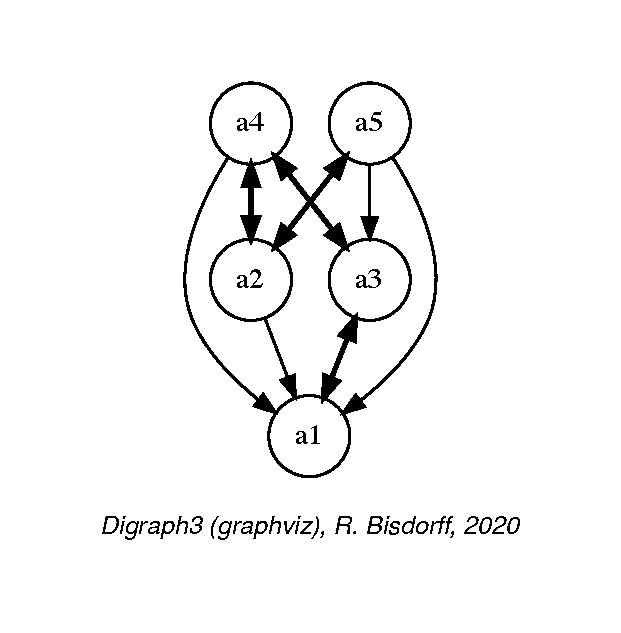
\includegraphics[width=7cm]{Figures/1-1-tutorialDigraph.pdf}
\caption[The tutorial crisp digraph]{The tutorial crisp digraph. The \texttt{exportGraphViz()} method is depending on drawing tools from \texttt{https://graphviz.org}. On Linux Ubuntu or Debian you may try '\texttt{sudo apt-get install graphviz}’ to install them. For Mac OSX There are ready $dmg$ installers available}
\label{fig:1.1}       % Give a unique label
\end{figure}

Further methods are provided for inspecting this random \texttt{Digraph} object \texttt{dg}, like the following \texttt{showStatistics()}\index{showStatistics@\texttt{showStatistics()}} method.
\begin{lstlisting}[caption={Inspecting a \texttt{Digraph} object},label=list:1.5]
>>> dg.showStatistics()
 *----- general statistics -------------*
 for digraph              : <tutorialDigraph.py>
 order                    : 5 nodes
 size                     : 12 arcs
 undetermined           : 0 arcs
 determinateness (%)      : 100.0
 arc density              : 0.60
 double arc density       : 0.40
 single arc density       : 0.40
 absence density          : 0.20
 strict single arc density: 0.40
 strict absence density   : 0.20
 nbr. of components         : 1
 nbr. of strong components  : 1
 transitivity degree (%)  : 60.0
                          : [0, 1, 2, 3, 4, 5]
 outdegrees distribution  : [0, 1, 1, 3, 0, 0]
 indegrees distribution   : [0, 1, 2, 1, 1, 0]
 mean outdegree           : 2.40
 mean indegree            : 2.40
                          : [0, 1, 2, 3, 4, 5, 6, 7, 8, 9, 10]
 symmetric degrees dist.  : [0, 0, 0, 0, 1, 4, 0, 0, 0, 0, 0]
 mean symmetric degree    : 4.80
 outdegrees concentration index   : 0.1667
 indegrees concentration index    : 0.2333
 symdegrees concentration index   : 0.0333
                                  : [0, 1, 2, 3, 4, 'inf']
 neighbourhood depths distribution: [0, 1, 4, 0, 0, 0]
 mean neighbourhood depth         : 1.80
 digraph diameter                 : 2
 agglomeration distribution       :
 a1 : 58.33
 a2 : 33.33
 a3 : 33.33
 a4 : 50.00
 a5 : 50.00
 agglomeration coefficient        : 45.00
\end{lstlisting}

The preceding \texttt{show...()} methods usually rely upon corresponding compute methods, like: \texttt{computeSize()}\index{computeSize@\texttt{computeSize()}}, \texttt{computeDeterminateness()}\index{computeDeterminateness@\texttt{computeDeterminateness()}},\\ or \texttt{computeTransitivityDegree()}\index{computeTransitivityDegree@\texttt{computeTransitivityDegree()}}.
\begin{lstlisting}[caption={Various \texttt{compute...()} methods.},label=list:1.6]
>>> dg.computeSize()
 12
>>> dg.computeDeterminateness(InPercents=True)
 Decimal('100.00')
>>> dg.computeTransitivityDegree(InPercents=True)
 Decimal('60.00')
\end{lstlisting}

Mind that \texttt{show...()} methods output their results in the \emph{Python} console. We provide also some \texttt{showHTML...()} methods which output their results in a system browser’s tab or window.
\begin{lstlisting}
>>> dg.showHTMLRelationMap(relationName='r(x,y)',\
...                        rankingRule=None)
\end{lstlisting}
\begin{figure}[ht]
\sidecaption[t]
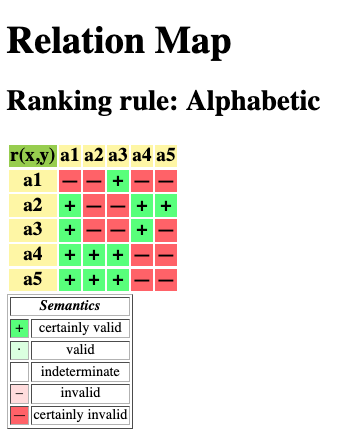
\includegraphics[width=5cm]{Figures/1-2-relationMap1.png}
\caption[Browsing the relation map of the tutorial digraph]{Browsing the relation map of the tutorial digraph. $+$ indicates a certainly valid and $-$ indicates a certainly  invalid relation, Here we find confirmed again that our random digraph instance \texttt{dg}, is indeed a crisp, i.e. $100\%$ determined irreflexive digraph instance}
\label{fig:1.2}       % Give a unique label
\end{figure}

% \section{Special digraph instances}
% \label{sec:1.5}

Some special types of digraph instances, like the \texttt{CirculantDigraph}\index{CirculantDigraph@\texttt{CirculantDigraph} class} or the \texttt{GridDigraph}\index{GridDigraph@\texttt{GridDigraph} class} classes, are readily available (see Fig.~\vref{fig:1.3}).
 \begin{figure}[ht]
%\sidecaption[t]
  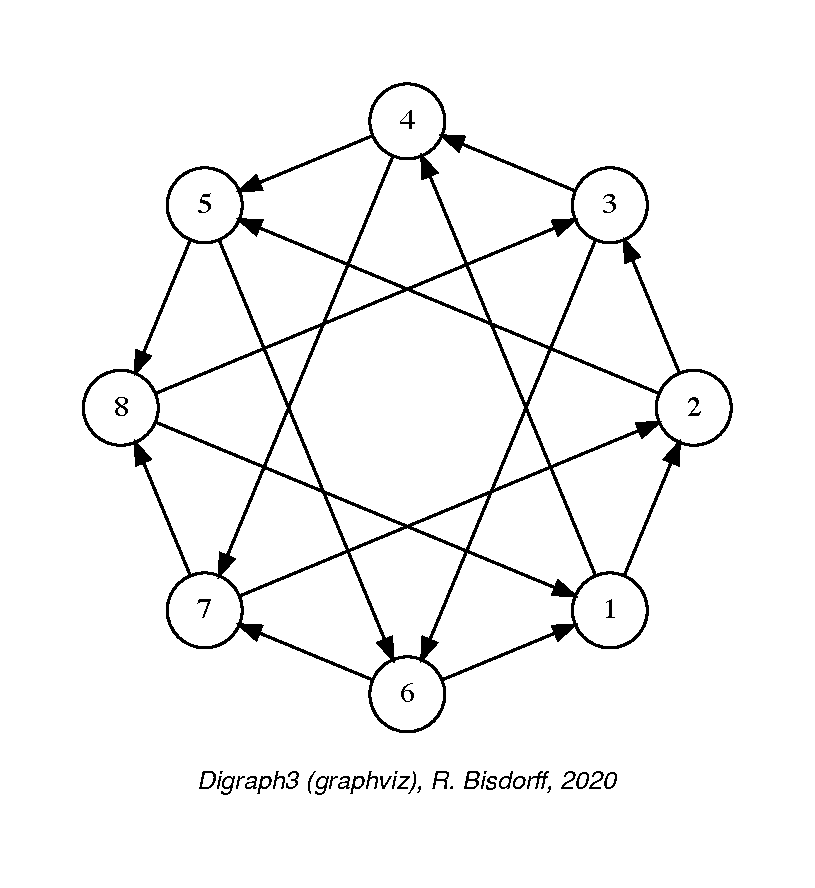
\includegraphics[height=6cm]{Figures/1-3-c8.pdf} \hfill
  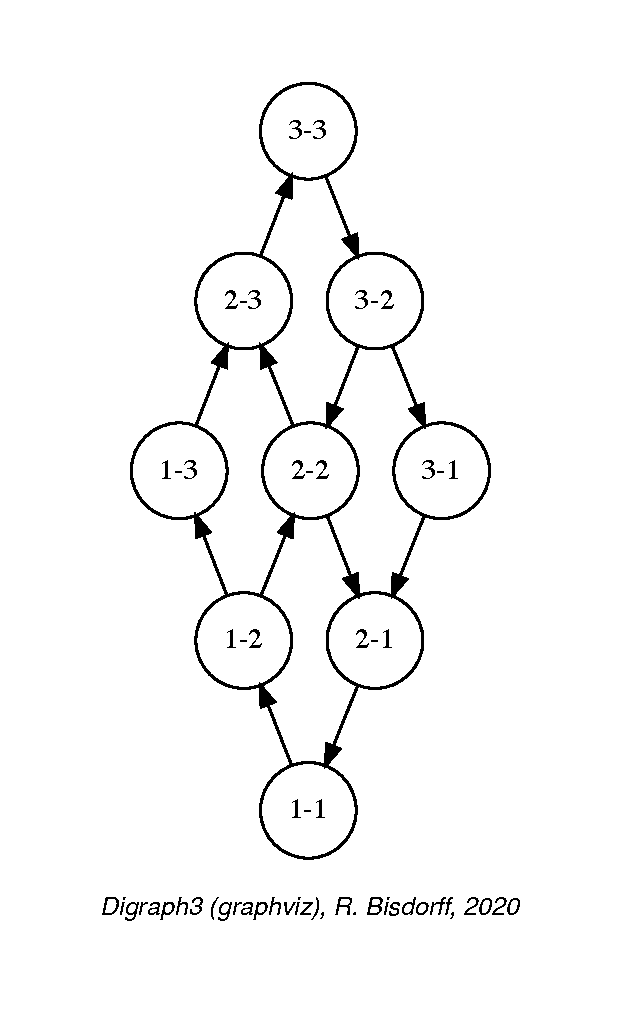
\includegraphics[height=6cm]{Figures/1-3-grid3.pdf} \hfill
  \caption{The circulant [1,3] digraph and the 3x3 grid digraph}
\label{fig:1.3}       % Give a unique label
\end{figure}
\begin{lstlisting}[caption={Circulant digraphs and $n \times m$ grid digraphs},label=list:1.7]
>>> from digraphs import CirculantDigraph,GridDigraph
>>> c8 = CirculantDigraph(order=8,circulants=[1,3])
>>> c8.exportGraphViz('c8')
  *---- exporting a dot file for GraphViz tools ----*
   Exporting to c8.dot
   circo -Tpng c8.dot -o c8.png
>>> grid3 = GridDigraph(n=3,m=3,\
...                    hasMedianSplitOrientation=True)
>>> grid.exportGraphViz('grid3')
  *---- exporting a dot file for GraphViz tools ----*
   Exporting to grid3.dot
   dot -Grankdir=BT -Tpng grid3.dot -o grid3.png
 \end{lstlisting}

%\vspace{1cm}
\vspace{\baselineskip}
The next Chapter~\ref{sec:2} will introduce the fondamental \emph{bipolar-valued digraph} model which is \emph{root object type} to all the digraph models implemented in the \Digraph modules \citep{BIS-2021b}.    

%%%%%%% The chapter bibliography
% % \normallatexbib
%\phantomsection
%\addcontentsline{toc}{section}{Chapter Bibliography}
%%%%%%%%%%%%%%%%%%%%%% chapter.tex %%%%%%%%%%%%%%%%%%%%%%%%%%%%%%%%%
%
% sample chapter
%
% Use this file as a template for your own input.
%
%%%%%%%%%%%%%%%%%%%%%%%% Springer-Verlag %%%%%%%%%%%%%%%%%%%%%%%%%%
%\motto{Use the template \emph{chapter.tex} to style the various elements of your chapter content.}
\chapter{Working with the \Digraph Python resources}
\label{sec:1} % chapter1
% use \chaptermark{}
% to alter or adjust the chapter heading in the running head

\abstract*{ The chapter is devoted to a first contact with the \Digraph Python resources. Following the installation instructions, we list the main Python modules with their purpose and eventually illustrate in a first Python terminal session how to generate, save and inspect a random crisp digraph.}

\abstract{ The chapter is devoted to a first contact with the \Digraph Python resources. Following the installation instructions, we list the main Python modules with their purpose and eventually illustrate in a first Python terminal session how to generate, save and inspect a random crisp digraph.}

\section{Installing the \Digraph resources}
\label{sec:1.1}

Using the \Digraph Python modules is easy\footnote{See the technical description of the \Digraph programming resources, \citet{BIS-2021b}.}. You only need to have installed on your system the Python programming language of version 3 (readily available under Linux and Mac OS). Notice that, from Version 3.3 on, the Python standard \texttt{decimal} module implements very efficiently in C its \texttt{Decimal} class. Now, \texttt{Decimal} numbers are mainly used in the \Digraph characteristic valuation functions, which makes the recent \texttt{Python-3.7+} versions much faster (more than twice as fast) when extensive digraph operations are performed.
%\lstset{style=shstyle}
Several download options (easiest under Linux or Mac OS-X) are given; either, by using a git client and clone a working copy from the \texttt{github.com} directory:
\begin{lstlisting}[language=sh, backgroundcolor=\color{White}, numbers=none]
  ...$ git clone https://github.com/rbisdorff/Digraph3
\end{lstlisting}
or from the \texttt{sourceforge.net} directory:
\begin{lstlisting}[language=sh,backgroundcolor=\color{White},numbers=none]
  ...$ git clone https://git.code.sf.net/p/digraph3/code Digraph3
\end{lstlisting}

It is also possible with a browser access, to download either, from the \texttt{github.com} link or, from the \texttt{sourceforge.net} link above the latest distribution zip archive and extract it.

On Linux or Mac OS, \texttt{..\$ cd} to the cloned or extracted \texttt{Digraph3} directory. The following shell command installs (with \emph{sudo} !) the \Digraph modules in the current running python environment:
\begin{lstlisting}[language=sh, backgroundcolor=\color{White},numbers=none]
  .../Digraph3$ make install
\end{lstlisting}

Python-3.8 (or later) environment is recommended (see the \texttt{makefile} for adapting the \texttt{make install} command to your running python environment).

Whereas the following shell command installs the \Digraph modules in an activated virtual python environment:
\begin{lstlisting}[language=sh, backgroundcolor=\color{White}, numbers=none]
  .../Digraph3$ make installVenv
\end{lstlisting}


If the \emph{cython} \footnote{\href{https://cython.org}{https://cython.org}} C-compiled modules for Big Data applications are required, it is necessary to previously install the \emph{Cython} package in the running Python environment:
\begin{lstlisting}[language=sh, backgroundcolor=\color{White}, numbers=none]
  ...$ python3 -m pip install cython
\end{lstlisting}

It is recommended to run a test suite:
\begin{lstlisting}[language=sh, backgroundcolor=\color{White}, numbers=none]
  .../Digraph3$ make tests
\end{lstlisting}

Test results are stored in the \texttt{Digraph3/test} directory. Notice that the python3 \texttt{pytest} package is required:
\begin{lstlisting}[language=sh, backgroundcolor=\color{White}, numbers=none]
  ...$ python3 -m pip install pytest
\end{lstlisting}

A verbose (with \texttt{stdout} not captured) \texttt{pytest} suite may be run as follows:
\begin{lstlisting}[language=sh, backgroundcolor=\color{White}, numbers=none]
  .../Digraph3$ make verboseTests
\end{lstlisting}

When the GNU \texttt{parallel} shell tool\index{parallel@\texttt{parallel} shell tool}\footnote{\href{https://www.gnu.org/software/parallel}{https://www.gnu.org/software/parallel}} is installed and multiple cores are detected, the tests may be executed in multiple processing mode:
\begin{lstlisting}[language=sh, backgroundcolor=\color{White}, numbers=none]
  ../Digraph3$ make pTests
\end{lstlisting}

Individual module \texttt{pytest} suites are also provided (see the \texttt{makefile}), like the one for the \texttt{outrankingDigraphs} module (see Chap.~\ref{sec:2}):
\begin{lstlisting}[language=sh, backgroundcolor=\color{White}, numbers=none]
../Digraph3$ make outrankingDigraphsTests
\end{lstlisting}

\paragraph{\textbf{Dependencies:}}

\noindent To be fully functional, the \Digraph resources mainly need:
\begin{itemize}[leftmargin=0.5cm,listparindent=0em,rightmargin=0.2cm,topsep=1pt]
\item The \texttt{graphviz} tools \citep{graphviz}\footnote{\href{https://graphviz.org}{https://graphviz.org}}, and 
\item The R statistics resources \footnote{\href{https://www.r-project.org}{https://www.r-project.org}} to be installed.
\item When exploring digraph isomorphisms, the \texttt{nauty} isomorphism testing program is required \citep*{nauty}. On linux you may try: \texttt{sudo apt install nauty}. For Mac OS X, corresponding \texttt{dmg} installers are available for downloading.
\item Two specific methods of the \texttt{OutrankingDigraph} class for clustering performance criteria or decision alternatives require furthermore the \texttt{calmat} matrix computing resource to be installed (see the \texttt{calmat} directory in the \Digraph resources).
\end{itemize}

\section{Organisation of the \Digraph Python modules}
\label{sec:1.2}

The main data handling modules of the \Digraph resources are the following:
\begin{enumerate}[leftmargin=0.75cm]
\item \texttt{digraphs}: main part of the \Digraph source code with the root \texttt{Digraph} class.
\item \texttt{graphs}: resources for handling undirected graphs with the root \texttt{Graph} class and a bridge to the \texttt{digraphs} module resources.
\item \texttt{perfTabs}: tools for handling multiple-criteria performance tableaux with root \texttt{PerformanceTableau} class.
\item \texttt{outrankingDigraphs}: root module for handling outranking digraphs with the abstract root \texttt{OutrankingDigraph} class and the main \texttt{Bipolar\-OutrankingDigraph} class. \footnote{Notice that the outrankingDigraph class defines a hybrid object type, inheriting conjointly from the \texttt{Digraph} class and the \texttt{PerformanceTableau} class.}
\item \texttt{votingProfiles}: classes and methods for handling voting ballots and computing election results with main \texttt{LinearVotingProfile} class.
\end{enumerate}

\noindent Various random generators are provided by the following modules:
\begin{enumerate}[leftmargin=0.75cm]
\item \texttt{randomDigraphs}: various random digraph models like random crisp digraphs (\texttt{RandomDigraph} class) or random bipolar-valued digraphs (\texttt{Random\-ValuationDigraph} class).
\item \texttt{randomPerfTabs}: various implemented random performance tableau models, like Cost-Benefit tableaux (\texttt{RandomCBPerformance\-Tableau} class) or 3-Objectives tableaux (\texttt{Random3ObjectivesPer\-formance\-Tableau} class).
\item \texttt{randomNumbers}: additional random number generators, not available in the standard Python \texttt{random.py} library, like a discrete random variable (\texttt{DiscreteRandomVariable} class) or a Cauchy random variable (\texttt{Cau\-chy\-RandomVariable} class)
\end{enumerate}

\noindent Following modules provide tools for \emph{sorting}, \emph{ranking} and \emph{rating} problems:
\begin{enumerate}[leftmargin=0.75cm]
\item \texttt{sortingDigraphs}: tools for solving sorting problems with the root \texttt{Sor\-tingDigraph} class and the main \texttt{QuantilesSortingDi\-graph} class;
\item \texttt{linearOrders}: tools for solving linearly ranking or ordering problems with the root \texttt{LinearOrder} class;
\item \texttt{transitiveDigraphs}: additional tools for handing transitive digraphs with root \texttt{TransitiveDigraph} class.
\end{enumerate}

\noindent Tools for specifically handling Big Data are eventually provided by the following modules:
\begin{enumerate}[leftmargin=0.75cm]
\item \texttt{performanceQuantiles}: incremental representation of large performance tableaux via binned cumulated density functions per criteria; Depends on the \texttt{randomPerfTabs} module.
\item \texttt{sparseOutrankingDigraphs}: sparse implementation design for bipolar-valued outranking digraphs of order $> 500$.
\item \emph{Cythonized} modules: C-compiled and optimised Python modules for handling big performance tableaux and bipolar outranking digraphs of order $> 1000$.
\end{enumerate}

Readers interested in technical implementation details are invited to consult the reference manual of the \Digraph resources, where they will find the documentation and complete source code of all \Digraph modules, classes and methods \citep{BIS-2021b}. 

\section{Starting a \Digraph terminal session}
\label{sec:1.3}
After downloading the \Digraph resources, one may start an interactive Python3 terminal session in the \texttt{Digraph3} directory.
\begin{lstlisting}[language=sh, backgroundcolor=\color{White}, numbers=none]
  $HOME/.../Digraph3$ python3
  Python 3.9.6 (v3.9.6:db3ff76da1, Jun 28 2021, 11:49:53) 
  [Clang 6.0 (clang-600.0.57)] on darwin
  Type "help", "copyright", "credits" or 
     "license" for more information.
  >>>
\end{lstlisting}

For exploring the classes and methods provided by the \Digraph modules enter the Python3 commands following the session prompts marked with $>>>$ or \texttt{...}; the lines without a prompt are output from the Python3 interpreter. Python class names and boolean parameters start by convention with a capital case; names of other Python objects, like modules, methods and variables start with a lower case. All Python names and code are shown in a \texttt{typewriting} font.
\begin{lstlisting}[caption={Generating a digraph instance},label=list:1.1]
>>> from randomDigraphs import RandomDigraph
>>> dg = RandomDigraph(order=5,arcProbability=0.5,\
...                    seed=101)
>>> dg
  *------- Digraph instance description ------*
   Instance class      : RandomDigraph
   Instance name       : randomDigraph
   Digraph Order       : 5
   Digraph Size        : 12
   Valuation domain    : [-1.00; 1.00]
   Determinateness (%) : 100.00
   Attributes       : ['actions','valuationdomain',
                       'relation','order','name',
                       'gamma','notGamma']
\end{lstlisting}

In Listing~\vref{list:1.1}  we import, for instance, from the \texttt{randomDigraphs}\index{randomDigraphs@\texttt{randomDigraphs} module} module the \texttt{RandomDigraph} class \index{RandomDigraph@\texttt{RandomDigraph} class} in order to generate a random digraph object \texttt{dg} of order 5 and arc probability of $50\%$. The resulting digraph of \emph{order} 5 --number of nodes called (decision) \emph{actions}-- and \emph{size} 12 --number of arcs-- is completely determined (see Line 11) .

% \section{Permanent storage of a digraph object}
% \label{sec:1.3}                   
The content of \texttt{dg} may be saved in a file named \texttt{tutorialDigraph.py}.
\begin{lstlisting}
>>> dg.save('tutorialDigraph')
 *--- Saving digraph in file: <tutorialDigraph.py> ---*
\end{lstlisting}
with the following content:
\begin{lstlisting}[caption={A stored digraph instance},label=list:1.2]
from decimal import Decimal
from collections import OrderedDict
actions = OrderedDict([
    ('a1', {'shortName': 'a1',
          'name': 'random decision action'}),
    ('a2', {'shortName': 'a2',
          'name': 'random decision action'}),
    ('a3', {'shortName': 'a3',
          'name': 'random decision action'}),
    ('a4', {'shortName': 'a4',
          'name': 'random decision action'}),
    ('a5', {'shortName': 'a5',
          'name': 'random decision action'}),
 ])
valuationdomain = {
     'min': Decimal('-1.0'),
     'med': Decimal('0.0'),
     'max': Decimal('1.0'),
     'hasIntegerValuation': True, # representation format
 }
relation = {
     'a1': {'a1':Decimal('-1.0'), 'a2':Decimal('-1.0'),
              'a3':Decimal('1.0'), 'a4':Decimal('-1.0'),
              'a5':Decimal('-1.0'),},
     'a2': {'a1':Decimal('1.0'), 'a2':Decimal('-1.0'),
              'a3':Decimal('-1.0'), 'a4':Decimal('1.0'),
              'a5':Decimal('1.0'),},
     'a3': {'a1':Decimal('1.0'), 'a2':Decimal('-1.0'),
              'a3':Decimal('-1.0'), 'a4':Decimal('1.0'),
              'a5':Decimal('-1.0'),},
     'a4': {'a1':Decimal('1.0'), 'a2':Decimal('1.0'),
              'a3':Decimal('1.0'), 'a4':Decimal('-1.0'),
              'a5':Decimal('-1.0'),},
     'a5': {'a1':Decimal('1.0'), 'a2':Decimal('1.0'),
              'a3':Decimal('1.0'), 'a4':Decimal('-1.0'),
              'a5':Decimal('-1.0'),},
 }
\end{lstlisting}

In the \Digraph resources, all digraph object instances are of root \texttt{Digraph}\index{Digraph@\texttt{Digraph} class} type (\href{https://digraph3.readthedocs.io/en/latest/techDoc.html#organisation-of-the-digraph3-modules}{see the technical description}) and contain at least the following attributes (see Listing~\vref{list:1.1}  Lines 12-14):
\begin{enumerate}[leftmargin=0.5cm,listparindent=0em,nosep]
\item A \texttt{name} attribute, holding usually the actual name of the stored instance that was used to create the instance;
\item An ordered dictionary of digraph nodes called \texttt{actions} (decision alternatives) with at least a \texttt{name} attribute;
\item An \texttt{order} attribute containing the number of graph nodes (length of the actions dictionary) automatically added by the object constructor;
\item  A logical characteristic \texttt{valuationdomain} dictionary with three decimal entries: the minimum ($-1.0$, means certainly false), the median ($0.0$, means missing information) and the maximum characteristic value ($+1.0$, means certainly true);
\item A double dictionary called \texttt{relation} and indexed by an oriented pair of actions (nodes) and carrying a decimal characteristic value in the range of the previous valuation domain;
\item Its associated \texttt{gamma } attribute, a dictionary containing the direct successors, respectively predecessors of each action, automatically added by the object constructor;
\item Its associated \texttt{notGamma} attribute, a dictionary containing the actions that are not direct successors respectively predecessors of each action, automatically added by the object constructor.
\end{enumerate}

\section{Inspecting a digraph object}
\label{sec:1.4}

Different \texttt{show...()} methods, like the \texttt{showShort()} method \index{showShort@\texttt{showShort()}}, reveal us now that \texttt{dg} is a crisp, irreflexive and connected digraph of order five (see List.~\vref{list:1.3}  Lines 1, 16, 26, 29).

\begin{lstlisting}[caption={Random crisp digraph object},label=list:1.3]
>>> dg.showShort()
 *----- show short -------------*
 Digraph          : tutorialDigraph
 Actions          : OrderedDict([
  ('a1', {'shortName': 'a1', 'name': 'random decision action'}),
  ('a2', {'shortName': 'a2', 'name': 'random decision action'}),
  ('a3', {'shortName': 'a3', 'name': 'random decision action'}),
  ('a4', {'shortName': 'a4', 'name': 'random decision action'}),
  ('a5', {'shortName': 'a5', 'name': 'random decision action'})
  ])
 Valuation domain : {
  'min': Decimal('-1.0'),
  'max': Decimal('1.0'),
  'med': Decimal('0.0'), 'hasIntegerValuation': True
  }
>>> dg.showRelationTable()
 * ---- Relation Table -----
   S   |  'a1'  'a2'  'a3'  'a4'  'a5'
 ------|-------------------------------
  'a1' |   -1    -1     1    -1    -1
  'a2' |    1    -1    -1     1     1
  'a3' |    1    -1    -1     1    -1
  'a4' |    1     1     1    -1    -1
  'a5' |    1     1     1    -1    -1
 Valuation domain: [-1;+1]
>>> dg.showComponents()
 *--- Connected Components ---*
 1: ['a1', 'a2', 'a3', 'a4', 'a5']
>>> dg.showNeighborhoods()
 Neighborhoods:
   Gamma     :
 'a1': in => {'a2', 'a4', 'a3', 'a5'}, out => {'a3'}
 'a2': in => {'a5', 'a4'}, out => {'a1', 'a4', 'a5'}
 'a3': in => {'a1', 'a4', 'a5'}, out => {'a1', 'a4'}
 'a4': in => {'a2', 'a3'}, out => {'a1', 'a3', 'a2'}
 'a5': in => {'a2'}, out => {'a1', 'a3', 'a2'}
   Not Gamma :
 'a1': in => set(), out => {'a2', 'a4', 'a5'}
 'a2': in => {'a1', 'a3'}, out => {'a3'}
 'a3': in => {'a2'}, out => {'a2', 'a5'}
 'a4': in => {'a1', 'a5'}, out => {'a5'}
 'a5': in => {'a1', 'a4', 'a3'}, out => {'a4'}
\end{lstlisting}

The \texttt{exportGraphViz()}\index{exportGraphViz@\texttt{exportGraphViz()}} method generates in the current working directory a \texttt{tutorialDigraph.dot} file and a \texttt{tutorialdigraph.png} picture of the tutorial digraph \texttt{dg} (see Fig.~\vref{fig:1.1}), if the \emph{graphviz} tools are installed on your system \citep{graphviz}.
\begin{lstlisting}
>>> dg.exportGraphViz('tutorialDigraph')
 *---- exporting a dot file do GraphViz tools ---------*
 Exporting to tutorialDigraph.dot
 dot -Grankdir=BT -Tpng tutorialDigraph.dot -o tutorialDigraph.png
\end{lstlisting}
\begin{figure}[ht]
\sidecaption[t]
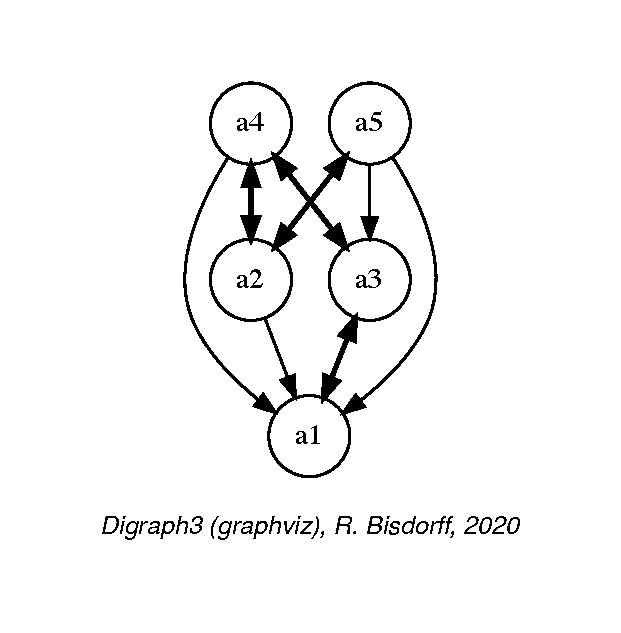
\includegraphics[width=7cm]{Figures/1-1-tutorialDigraph.pdf}
\caption[The tutorial crisp digraph]{The tutorial crisp digraph. The \texttt{exportGraphViz()} method is depending on drawing tools from \texttt{https://graphviz.org}. On Linux Ubuntu or Debian you may try '\texttt{sudo apt-get install graphviz}’ to install them. For Mac OSX There are ready $dmg$ installers available}
\label{fig:1.1}       % Give a unique label
\end{figure}

Further methods are provided for inspecting this random \texttt{Digraph} object \texttt{dg}, like the following \texttt{showStatistics()}\index{showStatistics@\texttt{showStatistics()}} method.
\begin{lstlisting}[caption={Inspecting a \texttt{Digraph} object},label=list:1.5]
>>> dg.showStatistics()
 *----- general statistics -------------*
 for digraph              : <tutorialDigraph.py>
 order                    : 5 nodes
 size                     : 12 arcs
 undetermined           : 0 arcs
 determinateness (%)      : 100.0
 arc density              : 0.60
 double arc density       : 0.40
 single arc density       : 0.40
 absence density          : 0.20
 strict single arc density: 0.40
 strict absence density   : 0.20
 nbr. of components         : 1
 nbr. of strong components  : 1
 transitivity degree (%)  : 60.0
                          : [0, 1, 2, 3, 4, 5]
 outdegrees distribution  : [0, 1, 1, 3, 0, 0]
 indegrees distribution   : [0, 1, 2, 1, 1, 0]
 mean outdegree           : 2.40
 mean indegree            : 2.40
                          : [0, 1, 2, 3, 4, 5, 6, 7, 8, 9, 10]
 symmetric degrees dist.  : [0, 0, 0, 0, 1, 4, 0, 0, 0, 0, 0]
 mean symmetric degree    : 4.80
 outdegrees concentration index   : 0.1667
 indegrees concentration index    : 0.2333
 symdegrees concentration index   : 0.0333
                                  : [0, 1, 2, 3, 4, 'inf']
 neighbourhood depths distribution: [0, 1, 4, 0, 0, 0]
 mean neighbourhood depth         : 1.80
 digraph diameter                 : 2
 agglomeration distribution       :
 a1 : 58.33
 a2 : 33.33
 a3 : 33.33
 a4 : 50.00
 a5 : 50.00
 agglomeration coefficient        : 45.00
\end{lstlisting}

The preceding \texttt{show...()} methods usually rely upon corresponding compute methods, like: \texttt{computeSize()}\index{computeSize@\texttt{computeSize()}}, \texttt{computeDeterminateness()}\index{computeDeterminateness@\texttt{computeDeterminateness()}},\\ or \texttt{computeTransitivityDegree()}\index{computeTransitivityDegree@\texttt{computeTransitivityDegree()}}.
\begin{lstlisting}[caption={Various \texttt{compute...()} methods.},label=list:1.6]
>>> dg.computeSize()
 12
>>> dg.computeDeterminateness(InPercents=True)
 Decimal('100.00')
>>> dg.computeTransitivityDegree(InPercents=True)
 Decimal('60.00')
\end{lstlisting}

Mind that \texttt{show...()} methods output their results in the \emph{Python} console. We provide also some \texttt{showHTML...()} methods which output their results in a system browser’s tab or window.
\begin{lstlisting}
>>> dg.showHTMLRelationMap(relationName='r(x,y)',\
...                        rankingRule=None)
\end{lstlisting}
\begin{figure}[ht]
\sidecaption[t]
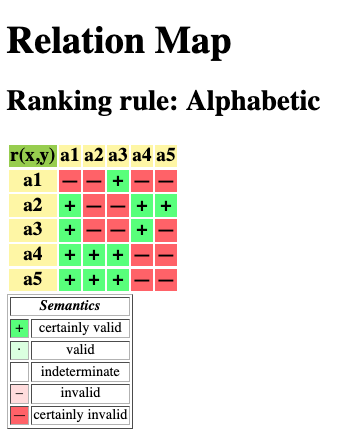
\includegraphics[width=5cm]{Figures/1-2-relationMap1.png}
\caption[Browsing the relation map of the tutorial digraph]{Browsing the relation map of the tutorial digraph. $+$ indicates a certainly valid and $-$ indicates a certainly  invalid relation, Here we find confirmed again that our random digraph instance \texttt{dg}, is indeed a crisp, i.e. $100\%$ determined irreflexive digraph instance}
\label{fig:1.2}       % Give a unique label
\end{figure}

% \section{Special digraph instances}
% \label{sec:1.5}

Some special types of digraph instances, like the \texttt{CirculantDigraph}\index{CirculantDigraph@\texttt{CirculantDigraph} class} or the \texttt{GridDigraph}\index{GridDigraph@\texttt{GridDigraph} class} classes, are readily available (see Fig.~\vref{fig:1.3}).
 \begin{figure}[ht]
%\sidecaption[t]
  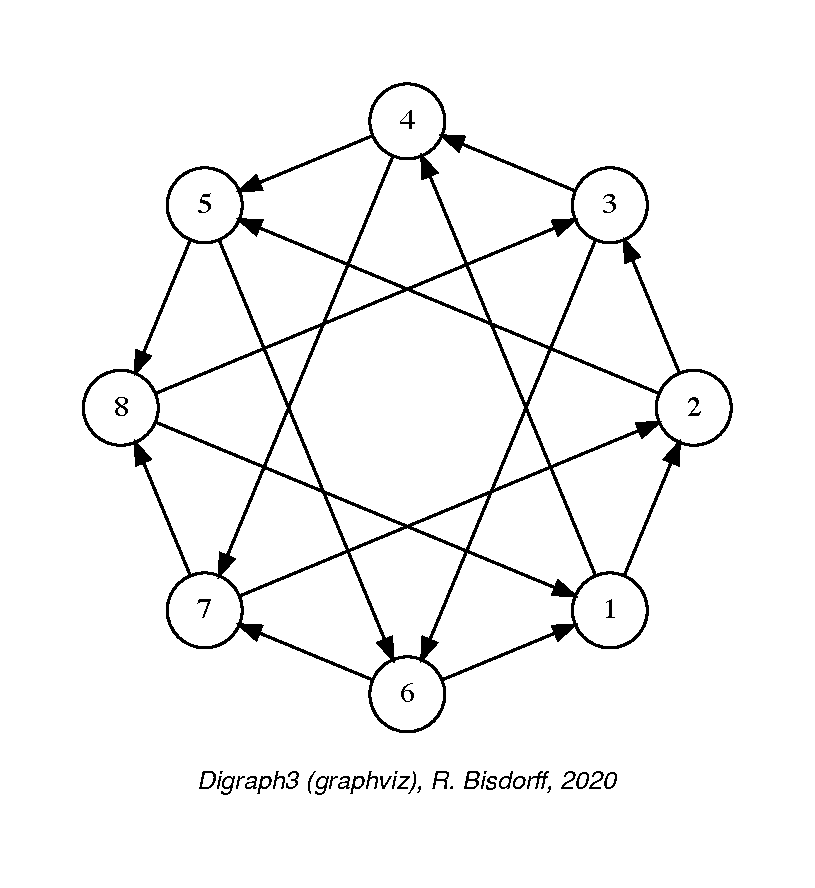
\includegraphics[height=6cm]{Figures/1-3-c8.pdf} \hfill
  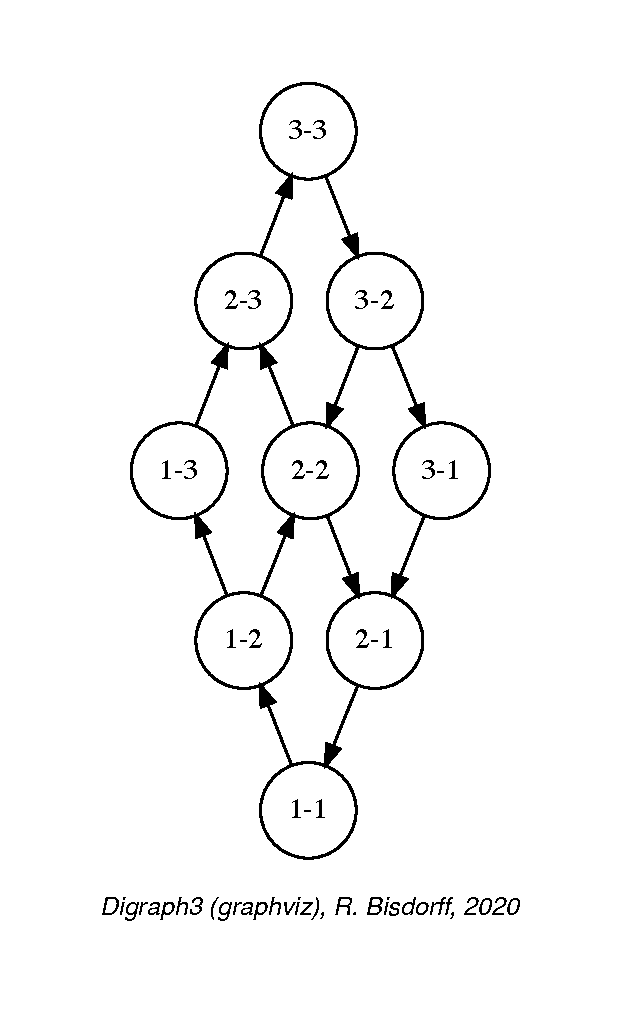
\includegraphics[height=6cm]{Figures/1-3-grid3.pdf} \hfill
  \caption{The circulant [1,3] digraph and the 3x3 grid digraph}
\label{fig:1.3}       % Give a unique label
\end{figure}
\begin{lstlisting}[caption={Circulant digraphs and $n \times m$ grid digraphs},label=list:1.7]
>>> from digraphs import CirculantDigraph,GridDigraph
>>> c8 = CirculantDigraph(order=8,circulants=[1,3])
>>> c8.exportGraphViz('c8')
  *---- exporting a dot file for GraphViz tools ----*
   Exporting to c8.dot
   circo -Tpng c8.dot -o c8.png
>>> grid3 = GridDigraph(n=3,m=3,\
...                    hasMedianSplitOrientation=True)
>>> grid.exportGraphViz('grid3')
  *---- exporting a dot file for GraphViz tools ----*
   Exporting to grid3.dot
   dot -Grankdir=BT -Tpng grid3.dot -o grid3.png
 \end{lstlisting}

%\vspace{1cm}
\vspace{\baselineskip}
The next Chapter~\ref{sec:2} will introduce the fondamental \emph{bipolar-valued digraph} model which is \emph{root object type} to all the digraph models implemented in the \Digraph modules \citep{BIS-2021b}.    

%%%%%%% The chapter bibliography
% % \normallatexbib
%\phantomsection
%\addcontentsline{toc}{section}{Chapter Bibliography}
%\input{02-mainMatters/01-chapterIntroDigraph3.bbl}
\bibliographystyle{spbasic}
\bibliography{03-backMatters/reference}

\bibliographystyle{spbasic}
\bibliography{03-backMatters/reference}


       
%%%%%%%%%%%%%%%%%%%%%part.tex%%%%%%%%%%%%%%%%%%%%%%%%%%%%%%%%%%
% 
% sample part title
%
% Use this file as a template for your own input.
%
%%%%%%%%%%%%%%%%%%%%%%%% Springer %%%%%%%%%%%%%%%%%%%%%%%%%%

\begin{partbacktext}
\part{Introduction to the \Digraph programming resources}
\noindent The first part contains three chapters for introducing the \Digraph software collection of Python programming resources. The first chapter is devoted to the installation of the \Digraph Python modules and running a first Python terminal session using the \Digraph3 resources. The second chapter introduces bipolar-valued digraphs, the root type of all available specialised digraphs. The third chapter finally introduces the main formal objects of this book, namely bipolar-valued outranking digraphs.
\end{partbacktext}
%%%%%%%%%%%%%%%%%%%%% chapter.tex %%%%%%%%%%%%%%%%%%%%%%%%%%%%%%%%%
%
% sample chapter
%
% Use this file as a template for your own input.
%
%%%%%%%%%%%%%%%%%%%%%%%% Springer-Verlag %%%%%%%%%%%%%%%%%%%%%%%%%%
%\motto{Use the template \emph{chapter.tex} to style the various elements of your chapter content.}
\chapter{Working with the \Digraph Python resources}
\label{sec:1} % chapter1
% use \chaptermark{}
% to alter or adjust the chapter heading in the running head

\abstract*{ The chapter is devoted to a first contact with the \Digraph Python resources. Following the installation instructions, we list the main Python modules with their purpose and eventually illustrate in a first Python terminal session how to generate, save and inspect a random crisp digraph.}

\abstract{ The chapter is devoted to a first contact with the \Digraph Python resources. Following the installation instructions, we list the main Python modules with their purpose and eventually illustrate in a first Python terminal session how to generate, save and inspect a random crisp digraph.}

\section{Installing the \Digraph resources}
\label{sec:1.1}

Using the \Digraph Python modules is easy\footnote{See the technical description of the \Digraph programming resources, \citet{BIS-2021b}.}. You only need to have installed on your system the Python programming language of version 3 (readily available under Linux and Mac OS). Notice that, from Version 3.3 on, the Python standard \texttt{decimal} module implements very efficiently in C its \texttt{Decimal} class. Now, \texttt{Decimal} numbers are mainly used in the \Digraph characteristic valuation functions, which makes the recent \texttt{Python-3.7+} versions much faster (more than twice as fast) when extensive digraph operations are performed.
%\lstset{style=shstyle}
Several download options (easiest under Linux or Mac OS-X) are given; either, by using a git client and clone a working copy from the \texttt{github.com} directory:
\begin{lstlisting}[language=sh, backgroundcolor=\color{White}, numbers=none]
  ...$ git clone https://github.com/rbisdorff/Digraph3
\end{lstlisting}
or from the \texttt{sourceforge.net} directory:
\begin{lstlisting}[language=sh,backgroundcolor=\color{White},numbers=none]
  ...$ git clone https://git.code.sf.net/p/digraph3/code Digraph3
\end{lstlisting}

It is also possible with a browser access, to download either, from the \texttt{github.com} link or, from the \texttt{sourceforge.net} link above the latest distribution zip archive and extract it.

On Linux or Mac OS, \texttt{..\$ cd} to the cloned or extracted \texttt{Digraph3} directory. The following shell command installs (with \emph{sudo} !) the \Digraph modules in the current running python environment:
\begin{lstlisting}[language=sh, backgroundcolor=\color{White},numbers=none]
  .../Digraph3$ make install
\end{lstlisting}

Python-3.8 (or later) environment is recommended (see the \texttt{makefile} for adapting the \texttt{make install} command to your running python environment).

Whereas the following shell command installs the \Digraph modules in an activated virtual python environment:
\begin{lstlisting}[language=sh, backgroundcolor=\color{White}, numbers=none]
  .../Digraph3$ make installVenv
\end{lstlisting}


If the \emph{cython} \footnote{\href{https://cython.org}{https://cython.org}} C-compiled modules for Big Data applications are required, it is necessary to previously install the \emph{Cython} package in the running Python environment:
\begin{lstlisting}[language=sh, backgroundcolor=\color{White}, numbers=none]
  ...$ python3 -m pip install cython
\end{lstlisting}

It is recommended to run a test suite:
\begin{lstlisting}[language=sh, backgroundcolor=\color{White}, numbers=none]
  .../Digraph3$ make tests
\end{lstlisting}

Test results are stored in the \texttt{Digraph3/test} directory. Notice that the python3 \texttt{pytest} package is required:
\begin{lstlisting}[language=sh, backgroundcolor=\color{White}, numbers=none]
  ...$ python3 -m pip install pytest
\end{lstlisting}

A verbose (with \texttt{stdout} not captured) \texttt{pytest} suite may be run as follows:
\begin{lstlisting}[language=sh, backgroundcolor=\color{White}, numbers=none]
  .../Digraph3$ make verboseTests
\end{lstlisting}

When the GNU \texttt{parallel} shell tool\index{parallel@\texttt{parallel} shell tool}\footnote{\href{https://www.gnu.org/software/parallel}{https://www.gnu.org/software/parallel}} is installed and multiple cores are detected, the tests may be executed in multiple processing mode:
\begin{lstlisting}[language=sh, backgroundcolor=\color{White}, numbers=none]
  ../Digraph3$ make pTests
\end{lstlisting}

Individual module \texttt{pytest} suites are also provided (see the \texttt{makefile}), like the one for the \texttt{outrankingDigraphs} module (see Chap.~\ref{sec:2}):
\begin{lstlisting}[language=sh, backgroundcolor=\color{White}, numbers=none]
../Digraph3$ make outrankingDigraphsTests
\end{lstlisting}

\paragraph{\textbf{Dependencies:}}

\noindent To be fully functional, the \Digraph resources mainly need:
\begin{itemize}[leftmargin=0.5cm,listparindent=0em,rightmargin=0.2cm,topsep=1pt]
\item The \texttt{graphviz} tools \citep{graphviz}\footnote{\href{https://graphviz.org}{https://graphviz.org}}, and 
\item The R statistics resources \footnote{\href{https://www.r-project.org}{https://www.r-project.org}} to be installed.
\item When exploring digraph isomorphisms, the \texttt{nauty} isomorphism testing program is required \citep*{nauty}. On linux you may try: \texttt{sudo apt install nauty}. For Mac OS X, corresponding \texttt{dmg} installers are available for downloading.
\item Two specific methods of the \texttt{OutrankingDigraph} class for clustering performance criteria or decision alternatives require furthermore the \texttt{calmat} matrix computing resource to be installed (see the \texttt{calmat} directory in the \Digraph resources).
\end{itemize}

\section{Organisation of the \Digraph Python modules}
\label{sec:1.2}

The main data handling modules of the \Digraph resources are the following:
\begin{enumerate}[leftmargin=0.75cm]
\item \texttt{digraphs}: main part of the \Digraph source code with the root \texttt{Digraph} class.
\item \texttt{graphs}: resources for handling undirected graphs with the root \texttt{Graph} class and a bridge to the \texttt{digraphs} module resources.
\item \texttt{perfTabs}: tools for handling multiple-criteria performance tableaux with root \texttt{PerformanceTableau} class.
\item \texttt{outrankingDigraphs}: root module for handling outranking digraphs with the abstract root \texttt{OutrankingDigraph} class and the main \texttt{Bipolar\-OutrankingDigraph} class. \footnote{Notice that the outrankingDigraph class defines a hybrid object type, inheriting conjointly from the \texttt{Digraph} class and the \texttt{PerformanceTableau} class.}
\item \texttt{votingProfiles}: classes and methods for handling voting ballots and computing election results with main \texttt{LinearVotingProfile} class.
\end{enumerate}

\noindent Various random generators are provided by the following modules:
\begin{enumerate}[leftmargin=0.75cm]
\item \texttt{randomDigraphs}: various random digraph models like random crisp digraphs (\texttt{RandomDigraph} class) or random bipolar-valued digraphs (\texttt{Random\-ValuationDigraph} class).
\item \texttt{randomPerfTabs}: various implemented random performance tableau models, like Cost-Benefit tableaux (\texttt{RandomCBPerformance\-Tableau} class) or 3-Objectives tableaux (\texttt{Random3ObjectivesPer\-formance\-Tableau} class).
\item \texttt{randomNumbers}: additional random number generators, not available in the standard Python \texttt{random.py} library, like a discrete random variable (\texttt{DiscreteRandomVariable} class) or a Cauchy random variable (\texttt{Cau\-chy\-RandomVariable} class)
\end{enumerate}

\noindent Following modules provide tools for \emph{sorting}, \emph{ranking} and \emph{rating} problems:
\begin{enumerate}[leftmargin=0.75cm]
\item \texttt{sortingDigraphs}: tools for solving sorting problems with the root \texttt{Sor\-tingDigraph} class and the main \texttt{QuantilesSortingDi\-graph} class;
\item \texttt{linearOrders}: tools for solving linearly ranking or ordering problems with the root \texttt{LinearOrder} class;
\item \texttt{transitiveDigraphs}: additional tools for handing transitive digraphs with root \texttt{TransitiveDigraph} class.
\end{enumerate}

\noindent Tools for specifically handling Big Data are eventually provided by the following modules:
\begin{enumerate}[leftmargin=0.75cm]
\item \texttt{performanceQuantiles}: incremental representation of large performance tableaux via binned cumulated density functions per criteria; Depends on the \texttt{randomPerfTabs} module.
\item \texttt{sparseOutrankingDigraphs}: sparse implementation design for bipolar-valued outranking digraphs of order $> 500$.
\item \emph{Cythonized} modules: C-compiled and optimised Python modules for handling big performance tableaux and bipolar outranking digraphs of order $> 1000$.
\end{enumerate}

Readers interested in technical implementation details are invited to consult the reference manual of the \Digraph resources, where they will find the documentation and complete source code of all \Digraph modules, classes and methods \citep{BIS-2021b}. 

\section{Starting a \Digraph terminal session}
\label{sec:1.3}
After downloading the \Digraph resources, one may start an interactive Python3 terminal session in the \texttt{Digraph3} directory.
\begin{lstlisting}[language=sh, backgroundcolor=\color{White}, numbers=none]
  $HOME/.../Digraph3$ python3
  Python 3.9.6 (v3.9.6:db3ff76da1, Jun 28 2021, 11:49:53) 
  [Clang 6.0 (clang-600.0.57)] on darwin
  Type "help", "copyright", "credits" or 
     "license" for more information.
  >>>
\end{lstlisting}

For exploring the classes and methods provided by the \Digraph modules enter the Python3 commands following the session prompts marked with $>>>$ or \texttt{...}; the lines without a prompt are output from the Python3 interpreter. Python class names and boolean parameters start by convention with a capital case; names of other Python objects, like modules, methods and variables start with a lower case. All Python names and code are shown in a \texttt{typewriting} font.
\begin{lstlisting}[caption={Generating a digraph instance},label=list:1.1]
>>> from randomDigraphs import RandomDigraph
>>> dg = RandomDigraph(order=5,arcProbability=0.5,\
...                    seed=101)
>>> dg
  *------- Digraph instance description ------*
   Instance class      : RandomDigraph
   Instance name       : randomDigraph
   Digraph Order       : 5
   Digraph Size        : 12
   Valuation domain    : [-1.00; 1.00]
   Determinateness (%) : 100.00
   Attributes       : ['actions','valuationdomain',
                       'relation','order','name',
                       'gamma','notGamma']
\end{lstlisting}

In Listing~\vref{list:1.1}  we import, for instance, from the \texttt{randomDigraphs}\index{randomDigraphs@\texttt{randomDigraphs} module} module the \texttt{RandomDigraph} class \index{RandomDigraph@\texttt{RandomDigraph} class} in order to generate a random digraph object \texttt{dg} of order 5 and arc probability of $50\%$. The resulting digraph of \emph{order} 5 --number of nodes called (decision) \emph{actions}-- and \emph{size} 12 --number of arcs-- is completely determined (see Line 11) .

% \section{Permanent storage of a digraph object}
% \label{sec:1.3}                   
The content of \texttt{dg} may be saved in a file named \texttt{tutorialDigraph.py}.
\begin{lstlisting}
>>> dg.save('tutorialDigraph')
 *--- Saving digraph in file: <tutorialDigraph.py> ---*
\end{lstlisting}
with the following content:
\begin{lstlisting}[caption={A stored digraph instance},label=list:1.2]
from decimal import Decimal
from collections import OrderedDict
actions = OrderedDict([
    ('a1', {'shortName': 'a1',
          'name': 'random decision action'}),
    ('a2', {'shortName': 'a2',
          'name': 'random decision action'}),
    ('a3', {'shortName': 'a3',
          'name': 'random decision action'}),
    ('a4', {'shortName': 'a4',
          'name': 'random decision action'}),
    ('a5', {'shortName': 'a5',
          'name': 'random decision action'}),
 ])
valuationdomain = {
     'min': Decimal('-1.0'),
     'med': Decimal('0.0'),
     'max': Decimal('1.0'),
     'hasIntegerValuation': True, # representation format
 }
relation = {
     'a1': {'a1':Decimal('-1.0'), 'a2':Decimal('-1.0'),
              'a3':Decimal('1.0'), 'a4':Decimal('-1.0'),
              'a5':Decimal('-1.0'),},
     'a2': {'a1':Decimal('1.0'), 'a2':Decimal('-1.0'),
              'a3':Decimal('-1.0'), 'a4':Decimal('1.0'),
              'a5':Decimal('1.0'),},
     'a3': {'a1':Decimal('1.0'), 'a2':Decimal('-1.0'),
              'a3':Decimal('-1.0'), 'a4':Decimal('1.0'),
              'a5':Decimal('-1.0'),},
     'a4': {'a1':Decimal('1.0'), 'a2':Decimal('1.0'),
              'a3':Decimal('1.0'), 'a4':Decimal('-1.0'),
              'a5':Decimal('-1.0'),},
     'a5': {'a1':Decimal('1.0'), 'a2':Decimal('1.0'),
              'a3':Decimal('1.0'), 'a4':Decimal('-1.0'),
              'a5':Decimal('-1.0'),},
 }
\end{lstlisting}

In the \Digraph resources, all digraph object instances are of root \texttt{Digraph}\index{Digraph@\texttt{Digraph} class} type (\href{https://digraph3.readthedocs.io/en/latest/techDoc.html#organisation-of-the-digraph3-modules}{see the technical description}) and contain at least the following attributes (see Listing~\vref{list:1.1}  Lines 12-14):
\begin{enumerate}[leftmargin=0.5cm,listparindent=0em,nosep]
\item A \texttt{name} attribute, holding usually the actual name of the stored instance that was used to create the instance;
\item An ordered dictionary of digraph nodes called \texttt{actions} (decision alternatives) with at least a \texttt{name} attribute;
\item An \texttt{order} attribute containing the number of graph nodes (length of the actions dictionary) automatically added by the object constructor;
\item  A logical characteristic \texttt{valuationdomain} dictionary with three decimal entries: the minimum ($-1.0$, means certainly false), the median ($0.0$, means missing information) and the maximum characteristic value ($+1.0$, means certainly true);
\item A double dictionary called \texttt{relation} and indexed by an oriented pair of actions (nodes) and carrying a decimal characteristic value in the range of the previous valuation domain;
\item Its associated \texttt{gamma } attribute, a dictionary containing the direct successors, respectively predecessors of each action, automatically added by the object constructor;
\item Its associated \texttt{notGamma} attribute, a dictionary containing the actions that are not direct successors respectively predecessors of each action, automatically added by the object constructor.
\end{enumerate}

\section{Inspecting a digraph object}
\label{sec:1.4}

Different \texttt{show...()} methods, like the \texttt{showShort()} method \index{showShort@\texttt{showShort()}}, reveal us now that \texttt{dg} is a crisp, irreflexive and connected digraph of order five (see List.~\vref{list:1.3}  Lines 1, 16, 26, 29).

\begin{lstlisting}[caption={Random crisp digraph object},label=list:1.3]
>>> dg.showShort()
 *----- show short -------------*
 Digraph          : tutorialDigraph
 Actions          : OrderedDict([
  ('a1', {'shortName': 'a1', 'name': 'random decision action'}),
  ('a2', {'shortName': 'a2', 'name': 'random decision action'}),
  ('a3', {'shortName': 'a3', 'name': 'random decision action'}),
  ('a4', {'shortName': 'a4', 'name': 'random decision action'}),
  ('a5', {'shortName': 'a5', 'name': 'random decision action'})
  ])
 Valuation domain : {
  'min': Decimal('-1.0'),
  'max': Decimal('1.0'),
  'med': Decimal('0.0'), 'hasIntegerValuation': True
  }
>>> dg.showRelationTable()
 * ---- Relation Table -----
   S   |  'a1'  'a2'  'a3'  'a4'  'a5'
 ------|-------------------------------
  'a1' |   -1    -1     1    -1    -1
  'a2' |    1    -1    -1     1     1
  'a3' |    1    -1    -1     1    -1
  'a4' |    1     1     1    -1    -1
  'a5' |    1     1     1    -1    -1
 Valuation domain: [-1;+1]
>>> dg.showComponents()
 *--- Connected Components ---*
 1: ['a1', 'a2', 'a3', 'a4', 'a5']
>>> dg.showNeighborhoods()
 Neighborhoods:
   Gamma     :
 'a1': in => {'a2', 'a4', 'a3', 'a5'}, out => {'a3'}
 'a2': in => {'a5', 'a4'}, out => {'a1', 'a4', 'a5'}
 'a3': in => {'a1', 'a4', 'a5'}, out => {'a1', 'a4'}
 'a4': in => {'a2', 'a3'}, out => {'a1', 'a3', 'a2'}
 'a5': in => {'a2'}, out => {'a1', 'a3', 'a2'}
   Not Gamma :
 'a1': in => set(), out => {'a2', 'a4', 'a5'}
 'a2': in => {'a1', 'a3'}, out => {'a3'}
 'a3': in => {'a2'}, out => {'a2', 'a5'}
 'a4': in => {'a1', 'a5'}, out => {'a5'}
 'a5': in => {'a1', 'a4', 'a3'}, out => {'a4'}
\end{lstlisting}

The \texttt{exportGraphViz()}\index{exportGraphViz@\texttt{exportGraphViz()}} method generates in the current working directory a \texttt{tutorialDigraph.dot} file and a \texttt{tutorialdigraph.png} picture of the tutorial digraph \texttt{dg} (see Fig.~\vref{fig:1.1}), if the \emph{graphviz} tools are installed on your system \citep{graphviz}.
\begin{lstlisting}
>>> dg.exportGraphViz('tutorialDigraph')
 *---- exporting a dot file do GraphViz tools ---------*
 Exporting to tutorialDigraph.dot
 dot -Grankdir=BT -Tpng tutorialDigraph.dot -o tutorialDigraph.png
\end{lstlisting}
\begin{figure}[ht]
\sidecaption[t]
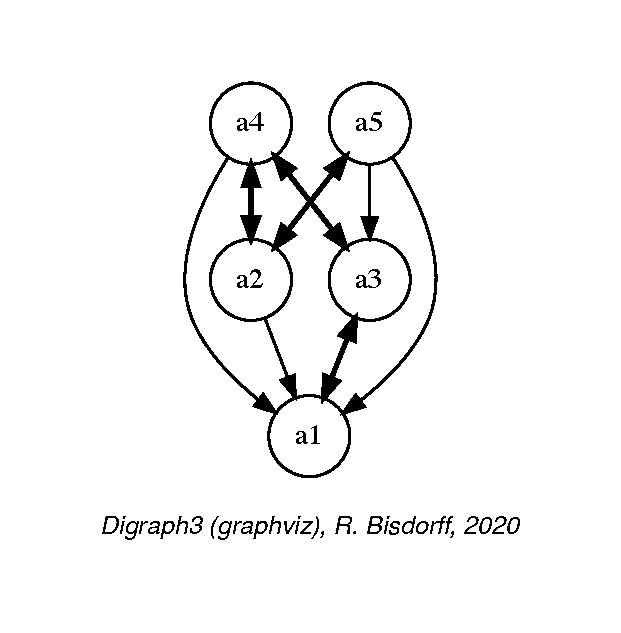
\includegraphics[width=7cm]{Figures/1-1-tutorialDigraph.pdf}
\caption[The tutorial crisp digraph]{The tutorial crisp digraph. The \texttt{exportGraphViz()} method is depending on drawing tools from \texttt{https://graphviz.org}. On Linux Ubuntu or Debian you may try '\texttt{sudo apt-get install graphviz}’ to install them. For Mac OSX There are ready $dmg$ installers available}
\label{fig:1.1}       % Give a unique label
\end{figure}

Further methods are provided for inspecting this random \texttt{Digraph} object \texttt{dg}, like the following \texttt{showStatistics()}\index{showStatistics@\texttt{showStatistics()}} method.
\begin{lstlisting}[caption={Inspecting a \texttt{Digraph} object},label=list:1.5]
>>> dg.showStatistics()
 *----- general statistics -------------*
 for digraph              : <tutorialDigraph.py>
 order                    : 5 nodes
 size                     : 12 arcs
 undetermined           : 0 arcs
 determinateness (%)      : 100.0
 arc density              : 0.60
 double arc density       : 0.40
 single arc density       : 0.40
 absence density          : 0.20
 strict single arc density: 0.40
 strict absence density   : 0.20
 nbr. of components         : 1
 nbr. of strong components  : 1
 transitivity degree (%)  : 60.0
                          : [0, 1, 2, 3, 4, 5]
 outdegrees distribution  : [0, 1, 1, 3, 0, 0]
 indegrees distribution   : [0, 1, 2, 1, 1, 0]
 mean outdegree           : 2.40
 mean indegree            : 2.40
                          : [0, 1, 2, 3, 4, 5, 6, 7, 8, 9, 10]
 symmetric degrees dist.  : [0, 0, 0, 0, 1, 4, 0, 0, 0, 0, 0]
 mean symmetric degree    : 4.80
 outdegrees concentration index   : 0.1667
 indegrees concentration index    : 0.2333
 symdegrees concentration index   : 0.0333
                                  : [0, 1, 2, 3, 4, 'inf']
 neighbourhood depths distribution: [0, 1, 4, 0, 0, 0]
 mean neighbourhood depth         : 1.80
 digraph diameter                 : 2
 agglomeration distribution       :
 a1 : 58.33
 a2 : 33.33
 a3 : 33.33
 a4 : 50.00
 a5 : 50.00
 agglomeration coefficient        : 45.00
\end{lstlisting}

The preceding \texttt{show...()} methods usually rely upon corresponding compute methods, like: \texttt{computeSize()}\index{computeSize@\texttt{computeSize()}}, \texttt{computeDeterminateness()}\index{computeDeterminateness@\texttt{computeDeterminateness()}},\\ or \texttt{computeTransitivityDegree()}\index{computeTransitivityDegree@\texttt{computeTransitivityDegree()}}.
\begin{lstlisting}[caption={Various \texttt{compute...()} methods.},label=list:1.6]
>>> dg.computeSize()
 12
>>> dg.computeDeterminateness(InPercents=True)
 Decimal('100.00')
>>> dg.computeTransitivityDegree(InPercents=True)
 Decimal('60.00')
\end{lstlisting}

Mind that \texttt{show...()} methods output their results in the \emph{Python} console. We provide also some \texttt{showHTML...()} methods which output their results in a system browser’s tab or window.
\begin{lstlisting}
>>> dg.showHTMLRelationMap(relationName='r(x,y)',\
...                        rankingRule=None)
\end{lstlisting}
\begin{figure}[ht]
\sidecaption[t]
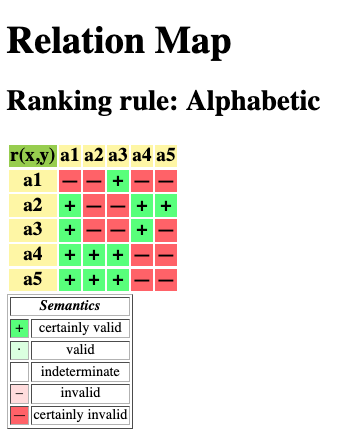
\includegraphics[width=5cm]{Figures/1-2-relationMap1.png}
\caption[Browsing the relation map of the tutorial digraph]{Browsing the relation map of the tutorial digraph. $+$ indicates a certainly valid and $-$ indicates a certainly  invalid relation, Here we find confirmed again that our random digraph instance \texttt{dg}, is indeed a crisp, i.e. $100\%$ determined irreflexive digraph instance}
\label{fig:1.2}       % Give a unique label
\end{figure}

% \section{Special digraph instances}
% \label{sec:1.5}

Some special types of digraph instances, like the \texttt{CirculantDigraph}\index{CirculantDigraph@\texttt{CirculantDigraph} class} or the \texttt{GridDigraph}\index{GridDigraph@\texttt{GridDigraph} class} classes, are readily available (see Fig.~\vref{fig:1.3}).
 \begin{figure}[ht]
%\sidecaption[t]
  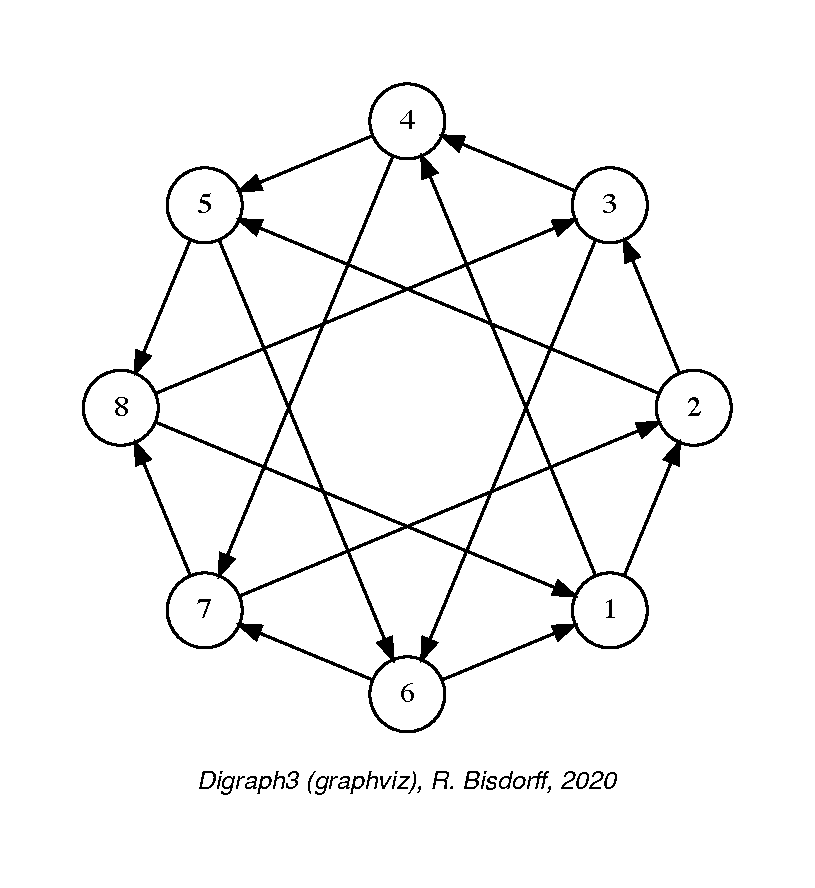
\includegraphics[height=6cm]{Figures/1-3-c8.pdf} \hfill
  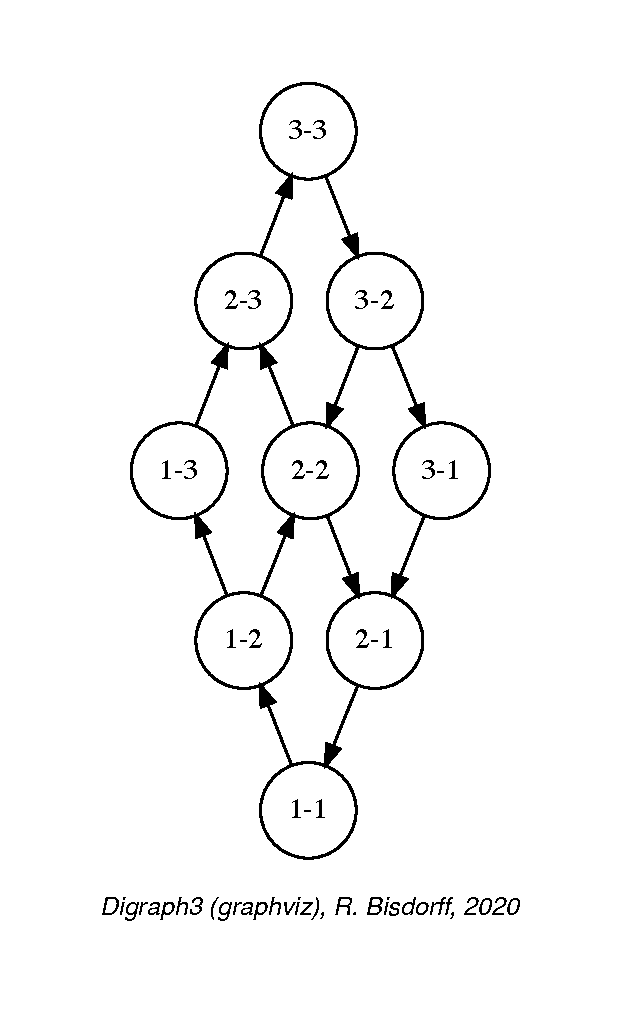
\includegraphics[height=6cm]{Figures/1-3-grid3.pdf} \hfill
  \caption{The circulant [1,3] digraph and the 3x3 grid digraph}
\label{fig:1.3}       % Give a unique label
\end{figure}
\begin{lstlisting}[caption={Circulant digraphs and $n \times m$ grid digraphs},label=list:1.7]
>>> from digraphs import CirculantDigraph,GridDigraph
>>> c8 = CirculantDigraph(order=8,circulants=[1,3])
>>> c8.exportGraphViz('c8')
  *---- exporting a dot file for GraphViz tools ----*
   Exporting to c8.dot
   circo -Tpng c8.dot -o c8.png
>>> grid3 = GridDigraph(n=3,m=3,\
...                    hasMedianSplitOrientation=True)
>>> grid.exportGraphViz('grid3')
  *---- exporting a dot file for GraphViz tools ----*
   Exporting to grid3.dot
   dot -Grankdir=BT -Tpng grid3.dot -o grid3.png
 \end{lstlisting}

%\vspace{1cm}
\vspace{\baselineskip}
The next Chapter~\ref{sec:2} will introduce the fondamental \emph{bipolar-valued digraph} model which is \emph{root object type} to all the digraph models implemented in the \Digraph modules \citep{BIS-2021b}.    

%%%%%%% The chapter bibliography
% % \normallatexbib
%\phantomsection
%\addcontentsline{toc}{section}{Chapter Bibliography}
%%%%%%%%%%%%%%%%%%%%%% chapter.tex %%%%%%%%%%%%%%%%%%%%%%%%%%%%%%%%%
%
% sample chapter
%
% Use this file as a template for your own input.
%
%%%%%%%%%%%%%%%%%%%%%%%% Springer-Verlag %%%%%%%%%%%%%%%%%%%%%%%%%%
%\motto{Use the template \emph{chapter.tex} to style the various elements of your chapter content.}
\chapter{Working with the \Digraph Python resources}
\label{sec:1} % chapter1
% use \chaptermark{}
% to alter or adjust the chapter heading in the running head

\abstract*{ The chapter is devoted to a first contact with the \Digraph Python resources. Following the installation instructions, we list the main Python modules with their purpose and eventually illustrate in a first Python terminal session how to generate, save and inspect a random crisp digraph.}

\abstract{ The chapter is devoted to a first contact with the \Digraph Python resources. Following the installation instructions, we list the main Python modules with their purpose and eventually illustrate in a first Python terminal session how to generate, save and inspect a random crisp digraph.}

\section{Installing the \Digraph resources}
\label{sec:1.1}

Using the \Digraph Python modules is easy\footnote{See the technical description of the \Digraph programming resources, \citet{BIS-2021b}.}. You only need to have installed on your system the Python programming language of version 3 (readily available under Linux and Mac OS). Notice that, from Version 3.3 on, the Python standard \texttt{decimal} module implements very efficiently in C its \texttt{Decimal} class. Now, \texttt{Decimal} numbers are mainly used in the \Digraph characteristic valuation functions, which makes the recent \texttt{Python-3.7+} versions much faster (more than twice as fast) when extensive digraph operations are performed.
%\lstset{style=shstyle}
Several download options (easiest under Linux or Mac OS-X) are given; either, by using a git client and clone a working copy from the \texttt{github.com} directory:
\begin{lstlisting}[language=sh, backgroundcolor=\color{White}, numbers=none]
  ...$ git clone https://github.com/rbisdorff/Digraph3
\end{lstlisting}
or from the \texttt{sourceforge.net} directory:
\begin{lstlisting}[language=sh,backgroundcolor=\color{White},numbers=none]
  ...$ git clone https://git.code.sf.net/p/digraph3/code Digraph3
\end{lstlisting}

It is also possible with a browser access, to download either, from the \texttt{github.com} link or, from the \texttt{sourceforge.net} link above the latest distribution zip archive and extract it.

On Linux or Mac OS, \texttt{..\$ cd} to the cloned or extracted \texttt{Digraph3} directory. The following shell command installs (with \emph{sudo} !) the \Digraph modules in the current running python environment:
\begin{lstlisting}[language=sh, backgroundcolor=\color{White},numbers=none]
  .../Digraph3$ make install
\end{lstlisting}

Python-3.8 (or later) environment is recommended (see the \texttt{makefile} for adapting the \texttt{make install} command to your running python environment).

Whereas the following shell command installs the \Digraph modules in an activated virtual python environment:
\begin{lstlisting}[language=sh, backgroundcolor=\color{White}, numbers=none]
  .../Digraph3$ make installVenv
\end{lstlisting}


If the \emph{cython} \footnote{\href{https://cython.org}{https://cython.org}} C-compiled modules for Big Data applications are required, it is necessary to previously install the \emph{Cython} package in the running Python environment:
\begin{lstlisting}[language=sh, backgroundcolor=\color{White}, numbers=none]
  ...$ python3 -m pip install cython
\end{lstlisting}

It is recommended to run a test suite:
\begin{lstlisting}[language=sh, backgroundcolor=\color{White}, numbers=none]
  .../Digraph3$ make tests
\end{lstlisting}

Test results are stored in the \texttt{Digraph3/test} directory. Notice that the python3 \texttt{pytest} package is required:
\begin{lstlisting}[language=sh, backgroundcolor=\color{White}, numbers=none]
  ...$ python3 -m pip install pytest
\end{lstlisting}

A verbose (with \texttt{stdout} not captured) \texttt{pytest} suite may be run as follows:
\begin{lstlisting}[language=sh, backgroundcolor=\color{White}, numbers=none]
  .../Digraph3$ make verboseTests
\end{lstlisting}

When the GNU \texttt{parallel} shell tool\index{parallel@\texttt{parallel} shell tool}\footnote{\href{https://www.gnu.org/software/parallel}{https://www.gnu.org/software/parallel}} is installed and multiple cores are detected, the tests may be executed in multiple processing mode:
\begin{lstlisting}[language=sh, backgroundcolor=\color{White}, numbers=none]
  ../Digraph3$ make pTests
\end{lstlisting}

Individual module \texttt{pytest} suites are also provided (see the \texttt{makefile}), like the one for the \texttt{outrankingDigraphs} module (see Chap.~\ref{sec:2}):
\begin{lstlisting}[language=sh, backgroundcolor=\color{White}, numbers=none]
../Digraph3$ make outrankingDigraphsTests
\end{lstlisting}

\paragraph{\textbf{Dependencies:}}

\noindent To be fully functional, the \Digraph resources mainly need:
\begin{itemize}[leftmargin=0.5cm,listparindent=0em,rightmargin=0.2cm,topsep=1pt]
\item The \texttt{graphviz} tools \citep{graphviz}\footnote{\href{https://graphviz.org}{https://graphviz.org}}, and 
\item The R statistics resources \footnote{\href{https://www.r-project.org}{https://www.r-project.org}} to be installed.
\item When exploring digraph isomorphisms, the \texttt{nauty} isomorphism testing program is required \citep*{nauty}. On linux you may try: \texttt{sudo apt install nauty}. For Mac OS X, corresponding \texttt{dmg} installers are available for downloading.
\item Two specific methods of the \texttt{OutrankingDigraph} class for clustering performance criteria or decision alternatives require furthermore the \texttt{calmat} matrix computing resource to be installed (see the \texttt{calmat} directory in the \Digraph resources).
\end{itemize}

\section{Organisation of the \Digraph Python modules}
\label{sec:1.2}

The main data handling modules of the \Digraph resources are the following:
\begin{enumerate}[leftmargin=0.75cm]
\item \texttt{digraphs}: main part of the \Digraph source code with the root \texttt{Digraph} class.
\item \texttt{graphs}: resources for handling undirected graphs with the root \texttt{Graph} class and a bridge to the \texttt{digraphs} module resources.
\item \texttt{perfTabs}: tools for handling multiple-criteria performance tableaux with root \texttt{PerformanceTableau} class.
\item \texttt{outrankingDigraphs}: root module for handling outranking digraphs with the abstract root \texttt{OutrankingDigraph} class and the main \texttt{Bipolar\-OutrankingDigraph} class. \footnote{Notice that the outrankingDigraph class defines a hybrid object type, inheriting conjointly from the \texttt{Digraph} class and the \texttt{PerformanceTableau} class.}
\item \texttt{votingProfiles}: classes and methods for handling voting ballots and computing election results with main \texttt{LinearVotingProfile} class.
\end{enumerate}

\noindent Various random generators are provided by the following modules:
\begin{enumerate}[leftmargin=0.75cm]
\item \texttt{randomDigraphs}: various random digraph models like random crisp digraphs (\texttt{RandomDigraph} class) or random bipolar-valued digraphs (\texttt{Random\-ValuationDigraph} class).
\item \texttt{randomPerfTabs}: various implemented random performance tableau models, like Cost-Benefit tableaux (\texttt{RandomCBPerformance\-Tableau} class) or 3-Objectives tableaux (\texttt{Random3ObjectivesPer\-formance\-Tableau} class).
\item \texttt{randomNumbers}: additional random number generators, not available in the standard Python \texttt{random.py} library, like a discrete random variable (\texttt{DiscreteRandomVariable} class) or a Cauchy random variable (\texttt{Cau\-chy\-RandomVariable} class)
\end{enumerate}

\noindent Following modules provide tools for \emph{sorting}, \emph{ranking} and \emph{rating} problems:
\begin{enumerate}[leftmargin=0.75cm]
\item \texttt{sortingDigraphs}: tools for solving sorting problems with the root \texttt{Sor\-tingDigraph} class and the main \texttt{QuantilesSortingDi\-graph} class;
\item \texttt{linearOrders}: tools for solving linearly ranking or ordering problems with the root \texttt{LinearOrder} class;
\item \texttt{transitiveDigraphs}: additional tools for handing transitive digraphs with root \texttt{TransitiveDigraph} class.
\end{enumerate}

\noindent Tools for specifically handling Big Data are eventually provided by the following modules:
\begin{enumerate}[leftmargin=0.75cm]
\item \texttt{performanceQuantiles}: incremental representation of large performance tableaux via binned cumulated density functions per criteria; Depends on the \texttt{randomPerfTabs} module.
\item \texttt{sparseOutrankingDigraphs}: sparse implementation design for bipolar-valued outranking digraphs of order $> 500$.
\item \emph{Cythonized} modules: C-compiled and optimised Python modules for handling big performance tableaux and bipolar outranking digraphs of order $> 1000$.
\end{enumerate}

Readers interested in technical implementation details are invited to consult the reference manual of the \Digraph resources, where they will find the documentation and complete source code of all \Digraph modules, classes and methods \citep{BIS-2021b}. 

\section{Starting a \Digraph terminal session}
\label{sec:1.3}
After downloading the \Digraph resources, one may start an interactive Python3 terminal session in the \texttt{Digraph3} directory.
\begin{lstlisting}[language=sh, backgroundcolor=\color{White}, numbers=none]
  $HOME/.../Digraph3$ python3
  Python 3.9.6 (v3.9.6:db3ff76da1, Jun 28 2021, 11:49:53) 
  [Clang 6.0 (clang-600.0.57)] on darwin
  Type "help", "copyright", "credits" or 
     "license" for more information.
  >>>
\end{lstlisting}

For exploring the classes and methods provided by the \Digraph modules enter the Python3 commands following the session prompts marked with $>>>$ or \texttt{...}; the lines without a prompt are output from the Python3 interpreter. Python class names and boolean parameters start by convention with a capital case; names of other Python objects, like modules, methods and variables start with a lower case. All Python names and code are shown in a \texttt{typewriting} font.
\begin{lstlisting}[caption={Generating a digraph instance},label=list:1.1]
>>> from randomDigraphs import RandomDigraph
>>> dg = RandomDigraph(order=5,arcProbability=0.5,\
...                    seed=101)
>>> dg
  *------- Digraph instance description ------*
   Instance class      : RandomDigraph
   Instance name       : randomDigraph
   Digraph Order       : 5
   Digraph Size        : 12
   Valuation domain    : [-1.00; 1.00]
   Determinateness (%) : 100.00
   Attributes       : ['actions','valuationdomain',
                       'relation','order','name',
                       'gamma','notGamma']
\end{lstlisting}

In Listing~\vref{list:1.1}  we import, for instance, from the \texttt{randomDigraphs}\index{randomDigraphs@\texttt{randomDigraphs} module} module the \texttt{RandomDigraph} class \index{RandomDigraph@\texttt{RandomDigraph} class} in order to generate a random digraph object \texttt{dg} of order 5 and arc probability of $50\%$. The resulting digraph of \emph{order} 5 --number of nodes called (decision) \emph{actions}-- and \emph{size} 12 --number of arcs-- is completely determined (see Line 11) .

% \section{Permanent storage of a digraph object}
% \label{sec:1.3}                   
The content of \texttt{dg} may be saved in a file named \texttt{tutorialDigraph.py}.
\begin{lstlisting}
>>> dg.save('tutorialDigraph')
 *--- Saving digraph in file: <tutorialDigraph.py> ---*
\end{lstlisting}
with the following content:
\begin{lstlisting}[caption={A stored digraph instance},label=list:1.2]
from decimal import Decimal
from collections import OrderedDict
actions = OrderedDict([
    ('a1', {'shortName': 'a1',
          'name': 'random decision action'}),
    ('a2', {'shortName': 'a2',
          'name': 'random decision action'}),
    ('a3', {'shortName': 'a3',
          'name': 'random decision action'}),
    ('a4', {'shortName': 'a4',
          'name': 'random decision action'}),
    ('a5', {'shortName': 'a5',
          'name': 'random decision action'}),
 ])
valuationdomain = {
     'min': Decimal('-1.0'),
     'med': Decimal('0.0'),
     'max': Decimal('1.0'),
     'hasIntegerValuation': True, # representation format
 }
relation = {
     'a1': {'a1':Decimal('-1.0'), 'a2':Decimal('-1.0'),
              'a3':Decimal('1.0'), 'a4':Decimal('-1.0'),
              'a5':Decimal('-1.0'),},
     'a2': {'a1':Decimal('1.0'), 'a2':Decimal('-1.0'),
              'a3':Decimal('-1.0'), 'a4':Decimal('1.0'),
              'a5':Decimal('1.0'),},
     'a3': {'a1':Decimal('1.0'), 'a2':Decimal('-1.0'),
              'a3':Decimal('-1.0'), 'a4':Decimal('1.0'),
              'a5':Decimal('-1.0'),},
     'a4': {'a1':Decimal('1.0'), 'a2':Decimal('1.0'),
              'a3':Decimal('1.0'), 'a4':Decimal('-1.0'),
              'a5':Decimal('-1.0'),},
     'a5': {'a1':Decimal('1.0'), 'a2':Decimal('1.0'),
              'a3':Decimal('1.0'), 'a4':Decimal('-1.0'),
              'a5':Decimal('-1.0'),},
 }
\end{lstlisting}

In the \Digraph resources, all digraph object instances are of root \texttt{Digraph}\index{Digraph@\texttt{Digraph} class} type (\href{https://digraph3.readthedocs.io/en/latest/techDoc.html#organisation-of-the-digraph3-modules}{see the technical description}) and contain at least the following attributes (see Listing~\vref{list:1.1}  Lines 12-14):
\begin{enumerate}[leftmargin=0.5cm,listparindent=0em,nosep]
\item A \texttt{name} attribute, holding usually the actual name of the stored instance that was used to create the instance;
\item An ordered dictionary of digraph nodes called \texttt{actions} (decision alternatives) with at least a \texttt{name} attribute;
\item An \texttt{order} attribute containing the number of graph nodes (length of the actions dictionary) automatically added by the object constructor;
\item  A logical characteristic \texttt{valuationdomain} dictionary with three decimal entries: the minimum ($-1.0$, means certainly false), the median ($0.0$, means missing information) and the maximum characteristic value ($+1.0$, means certainly true);
\item A double dictionary called \texttt{relation} and indexed by an oriented pair of actions (nodes) and carrying a decimal characteristic value in the range of the previous valuation domain;
\item Its associated \texttt{gamma } attribute, a dictionary containing the direct successors, respectively predecessors of each action, automatically added by the object constructor;
\item Its associated \texttt{notGamma} attribute, a dictionary containing the actions that are not direct successors respectively predecessors of each action, automatically added by the object constructor.
\end{enumerate}

\section{Inspecting a digraph object}
\label{sec:1.4}

Different \texttt{show...()} methods, like the \texttt{showShort()} method \index{showShort@\texttt{showShort()}}, reveal us now that \texttt{dg} is a crisp, irreflexive and connected digraph of order five (see List.~\vref{list:1.3}  Lines 1, 16, 26, 29).

\begin{lstlisting}[caption={Random crisp digraph object},label=list:1.3]
>>> dg.showShort()
 *----- show short -------------*
 Digraph          : tutorialDigraph
 Actions          : OrderedDict([
  ('a1', {'shortName': 'a1', 'name': 'random decision action'}),
  ('a2', {'shortName': 'a2', 'name': 'random decision action'}),
  ('a3', {'shortName': 'a3', 'name': 'random decision action'}),
  ('a4', {'shortName': 'a4', 'name': 'random decision action'}),
  ('a5', {'shortName': 'a5', 'name': 'random decision action'})
  ])
 Valuation domain : {
  'min': Decimal('-1.0'),
  'max': Decimal('1.0'),
  'med': Decimal('0.0'), 'hasIntegerValuation': True
  }
>>> dg.showRelationTable()
 * ---- Relation Table -----
   S   |  'a1'  'a2'  'a3'  'a4'  'a5'
 ------|-------------------------------
  'a1' |   -1    -1     1    -1    -1
  'a2' |    1    -1    -1     1     1
  'a3' |    1    -1    -1     1    -1
  'a4' |    1     1     1    -1    -1
  'a5' |    1     1     1    -1    -1
 Valuation domain: [-1;+1]
>>> dg.showComponents()
 *--- Connected Components ---*
 1: ['a1', 'a2', 'a3', 'a4', 'a5']
>>> dg.showNeighborhoods()
 Neighborhoods:
   Gamma     :
 'a1': in => {'a2', 'a4', 'a3', 'a5'}, out => {'a3'}
 'a2': in => {'a5', 'a4'}, out => {'a1', 'a4', 'a5'}
 'a3': in => {'a1', 'a4', 'a5'}, out => {'a1', 'a4'}
 'a4': in => {'a2', 'a3'}, out => {'a1', 'a3', 'a2'}
 'a5': in => {'a2'}, out => {'a1', 'a3', 'a2'}
   Not Gamma :
 'a1': in => set(), out => {'a2', 'a4', 'a5'}
 'a2': in => {'a1', 'a3'}, out => {'a3'}
 'a3': in => {'a2'}, out => {'a2', 'a5'}
 'a4': in => {'a1', 'a5'}, out => {'a5'}
 'a5': in => {'a1', 'a4', 'a3'}, out => {'a4'}
\end{lstlisting}

The \texttt{exportGraphViz()}\index{exportGraphViz@\texttt{exportGraphViz()}} method generates in the current working directory a \texttt{tutorialDigraph.dot} file and a \texttt{tutorialdigraph.png} picture of the tutorial digraph \texttt{dg} (see Fig.~\vref{fig:1.1}), if the \emph{graphviz} tools are installed on your system \citep{graphviz}.
\begin{lstlisting}
>>> dg.exportGraphViz('tutorialDigraph')
 *---- exporting a dot file do GraphViz tools ---------*
 Exporting to tutorialDigraph.dot
 dot -Grankdir=BT -Tpng tutorialDigraph.dot -o tutorialDigraph.png
\end{lstlisting}
\begin{figure}[ht]
\sidecaption[t]
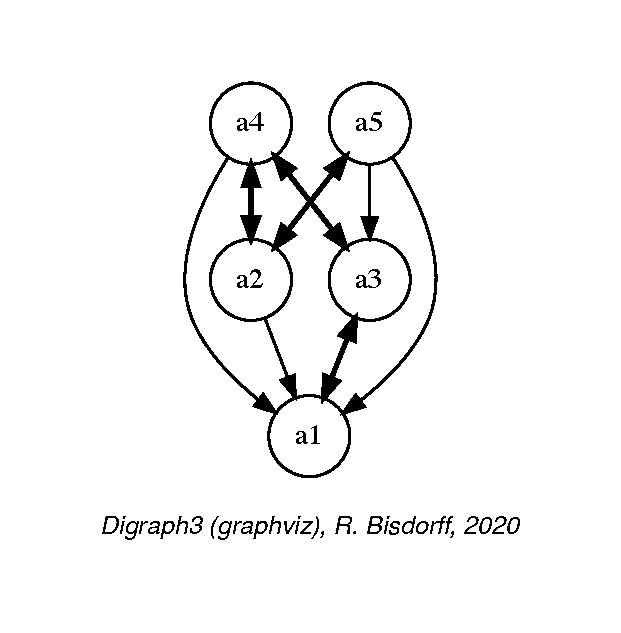
\includegraphics[width=7cm]{Figures/1-1-tutorialDigraph.pdf}
\caption[The tutorial crisp digraph]{The tutorial crisp digraph. The \texttt{exportGraphViz()} method is depending on drawing tools from \texttt{https://graphviz.org}. On Linux Ubuntu or Debian you may try '\texttt{sudo apt-get install graphviz}’ to install them. For Mac OSX There are ready $dmg$ installers available}
\label{fig:1.1}       % Give a unique label
\end{figure}

Further methods are provided for inspecting this random \texttt{Digraph} object \texttt{dg}, like the following \texttt{showStatistics()}\index{showStatistics@\texttt{showStatistics()}} method.
\begin{lstlisting}[caption={Inspecting a \texttt{Digraph} object},label=list:1.5]
>>> dg.showStatistics()
 *----- general statistics -------------*
 for digraph              : <tutorialDigraph.py>
 order                    : 5 nodes
 size                     : 12 arcs
 undetermined           : 0 arcs
 determinateness (%)      : 100.0
 arc density              : 0.60
 double arc density       : 0.40
 single arc density       : 0.40
 absence density          : 0.20
 strict single arc density: 0.40
 strict absence density   : 0.20
 nbr. of components         : 1
 nbr. of strong components  : 1
 transitivity degree (%)  : 60.0
                          : [0, 1, 2, 3, 4, 5]
 outdegrees distribution  : [0, 1, 1, 3, 0, 0]
 indegrees distribution   : [0, 1, 2, 1, 1, 0]
 mean outdegree           : 2.40
 mean indegree            : 2.40
                          : [0, 1, 2, 3, 4, 5, 6, 7, 8, 9, 10]
 symmetric degrees dist.  : [0, 0, 0, 0, 1, 4, 0, 0, 0, 0, 0]
 mean symmetric degree    : 4.80
 outdegrees concentration index   : 0.1667
 indegrees concentration index    : 0.2333
 symdegrees concentration index   : 0.0333
                                  : [0, 1, 2, 3, 4, 'inf']
 neighbourhood depths distribution: [0, 1, 4, 0, 0, 0]
 mean neighbourhood depth         : 1.80
 digraph diameter                 : 2
 agglomeration distribution       :
 a1 : 58.33
 a2 : 33.33
 a3 : 33.33
 a4 : 50.00
 a5 : 50.00
 agglomeration coefficient        : 45.00
\end{lstlisting}

The preceding \texttt{show...()} methods usually rely upon corresponding compute methods, like: \texttt{computeSize()}\index{computeSize@\texttt{computeSize()}}, \texttt{computeDeterminateness()}\index{computeDeterminateness@\texttt{computeDeterminateness()}},\\ or \texttt{computeTransitivityDegree()}\index{computeTransitivityDegree@\texttt{computeTransitivityDegree()}}.
\begin{lstlisting}[caption={Various \texttt{compute...()} methods.},label=list:1.6]
>>> dg.computeSize()
 12
>>> dg.computeDeterminateness(InPercents=True)
 Decimal('100.00')
>>> dg.computeTransitivityDegree(InPercents=True)
 Decimal('60.00')
\end{lstlisting}

Mind that \texttt{show...()} methods output their results in the \emph{Python} console. We provide also some \texttt{showHTML...()} methods which output their results in a system browser’s tab or window.
\begin{lstlisting}
>>> dg.showHTMLRelationMap(relationName='r(x,y)',\
...                        rankingRule=None)
\end{lstlisting}
\begin{figure}[ht]
\sidecaption[t]
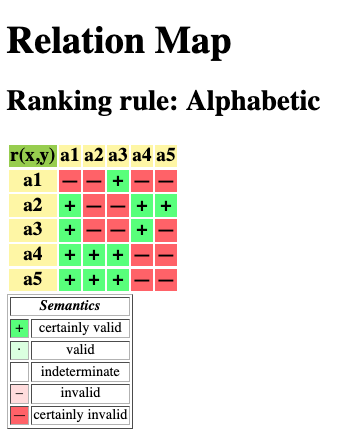
\includegraphics[width=5cm]{Figures/1-2-relationMap1.png}
\caption[Browsing the relation map of the tutorial digraph]{Browsing the relation map of the tutorial digraph. $+$ indicates a certainly valid and $-$ indicates a certainly  invalid relation, Here we find confirmed again that our random digraph instance \texttt{dg}, is indeed a crisp, i.e. $100\%$ determined irreflexive digraph instance}
\label{fig:1.2}       % Give a unique label
\end{figure}

% \section{Special digraph instances}
% \label{sec:1.5}

Some special types of digraph instances, like the \texttt{CirculantDigraph}\index{CirculantDigraph@\texttt{CirculantDigraph} class} or the \texttt{GridDigraph}\index{GridDigraph@\texttt{GridDigraph} class} classes, are readily available (see Fig.~\vref{fig:1.3}).
 \begin{figure}[ht]
%\sidecaption[t]
  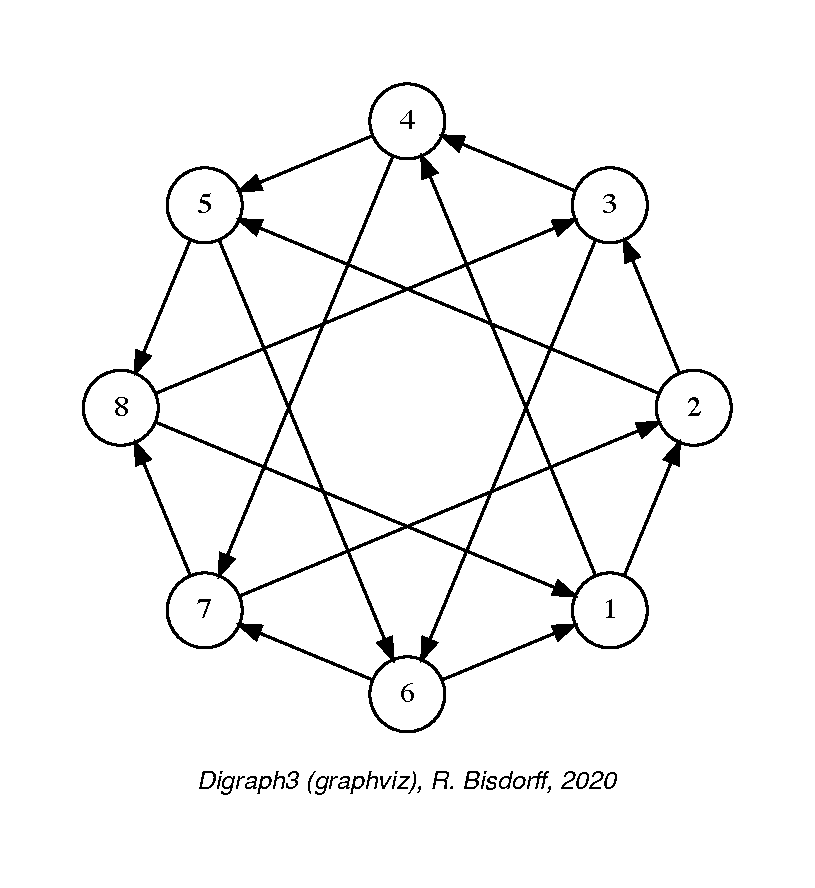
\includegraphics[height=6cm]{Figures/1-3-c8.pdf} \hfill
  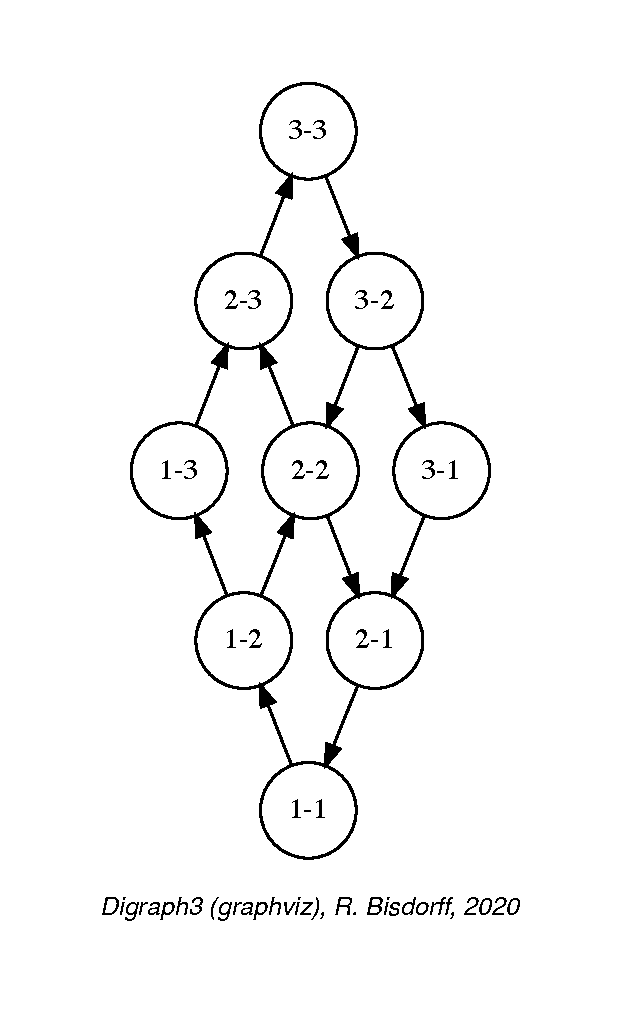
\includegraphics[height=6cm]{Figures/1-3-grid3.pdf} \hfill
  \caption{The circulant [1,3] digraph and the 3x3 grid digraph}
\label{fig:1.3}       % Give a unique label
\end{figure}
\begin{lstlisting}[caption={Circulant digraphs and $n \times m$ grid digraphs},label=list:1.7]
>>> from digraphs import CirculantDigraph,GridDigraph
>>> c8 = CirculantDigraph(order=8,circulants=[1,3])
>>> c8.exportGraphViz('c8')
  *---- exporting a dot file for GraphViz tools ----*
   Exporting to c8.dot
   circo -Tpng c8.dot -o c8.png
>>> grid3 = GridDigraph(n=3,m=3,\
...                    hasMedianSplitOrientation=True)
>>> grid.exportGraphViz('grid3')
  *---- exporting a dot file for GraphViz tools ----*
   Exporting to grid3.dot
   dot -Grankdir=BT -Tpng grid3.dot -o grid3.png
 \end{lstlisting}

%\vspace{1cm}
\vspace{\baselineskip}
The next Chapter~\ref{sec:2} will introduce the fondamental \emph{bipolar-valued digraph} model which is \emph{root object type} to all the digraph models implemented in the \Digraph modules \citep{BIS-2021b}.    

%%%%%%% The chapter bibliography
% % \normallatexbib
%\phantomsection
%\addcontentsline{toc}{section}{Chapter Bibliography}
%%%%%%%%%%%%%%%%%%%%%% chapter.tex %%%%%%%%%%%%%%%%%%%%%%%%%%%%%%%%%
%
% sample chapter
%
% Use this file as a template for your own input.
%
%%%%%%%%%%%%%%%%%%%%%%%% Springer-Verlag %%%%%%%%%%%%%%%%%%%%%%%%%%
%\motto{Use the template \emph{chapter.tex} to style the various elements of your chapter content.}
\chapter{Working with the \Digraph Python resources}
\label{sec:1} % chapter1
% use \chaptermark{}
% to alter or adjust the chapter heading in the running head

\abstract*{ The chapter is devoted to a first contact with the \Digraph Python resources. Following the installation instructions, we list the main Python modules with their purpose and eventually illustrate in a first Python terminal session how to generate, save and inspect a random crisp digraph.}

\abstract{ The chapter is devoted to a first contact with the \Digraph Python resources. Following the installation instructions, we list the main Python modules with their purpose and eventually illustrate in a first Python terminal session how to generate, save and inspect a random crisp digraph.}

\section{Installing the \Digraph resources}
\label{sec:1.1}

Using the \Digraph Python modules is easy\footnote{See the technical description of the \Digraph programming resources, \citet{BIS-2021b}.}. You only need to have installed on your system the Python programming language of version 3 (readily available under Linux and Mac OS). Notice that, from Version 3.3 on, the Python standard \texttt{decimal} module implements very efficiently in C its \texttt{Decimal} class. Now, \texttt{Decimal} numbers are mainly used in the \Digraph characteristic valuation functions, which makes the recent \texttt{Python-3.7+} versions much faster (more than twice as fast) when extensive digraph operations are performed.
%\lstset{style=shstyle}
Several download options (easiest under Linux or Mac OS-X) are given; either, by using a git client and clone a working copy from the \texttt{github.com} directory:
\begin{lstlisting}[language=sh, backgroundcolor=\color{White}, numbers=none]
  ...$ git clone https://github.com/rbisdorff/Digraph3
\end{lstlisting}
or from the \texttt{sourceforge.net} directory:
\begin{lstlisting}[language=sh,backgroundcolor=\color{White},numbers=none]
  ...$ git clone https://git.code.sf.net/p/digraph3/code Digraph3
\end{lstlisting}

It is also possible with a browser access, to download either, from the \texttt{github.com} link or, from the \texttt{sourceforge.net} link above the latest distribution zip archive and extract it.

On Linux or Mac OS, \texttt{..\$ cd} to the cloned or extracted \texttt{Digraph3} directory. The following shell command installs (with \emph{sudo} !) the \Digraph modules in the current running python environment:
\begin{lstlisting}[language=sh, backgroundcolor=\color{White},numbers=none]
  .../Digraph3$ make install
\end{lstlisting}

Python-3.8 (or later) environment is recommended (see the \texttt{makefile} for adapting the \texttt{make install} command to your running python environment).

Whereas the following shell command installs the \Digraph modules in an activated virtual python environment:
\begin{lstlisting}[language=sh, backgroundcolor=\color{White}, numbers=none]
  .../Digraph3$ make installVenv
\end{lstlisting}


If the \emph{cython} \footnote{\href{https://cython.org}{https://cython.org}} C-compiled modules for Big Data applications are required, it is necessary to previously install the \emph{Cython} package in the running Python environment:
\begin{lstlisting}[language=sh, backgroundcolor=\color{White}, numbers=none]
  ...$ python3 -m pip install cython
\end{lstlisting}

It is recommended to run a test suite:
\begin{lstlisting}[language=sh, backgroundcolor=\color{White}, numbers=none]
  .../Digraph3$ make tests
\end{lstlisting}

Test results are stored in the \texttt{Digraph3/test} directory. Notice that the python3 \texttt{pytest} package is required:
\begin{lstlisting}[language=sh, backgroundcolor=\color{White}, numbers=none]
  ...$ python3 -m pip install pytest
\end{lstlisting}

A verbose (with \texttt{stdout} not captured) \texttt{pytest} suite may be run as follows:
\begin{lstlisting}[language=sh, backgroundcolor=\color{White}, numbers=none]
  .../Digraph3$ make verboseTests
\end{lstlisting}

When the GNU \texttt{parallel} shell tool\index{parallel@\texttt{parallel} shell tool}\footnote{\href{https://www.gnu.org/software/parallel}{https://www.gnu.org/software/parallel}} is installed and multiple cores are detected, the tests may be executed in multiple processing mode:
\begin{lstlisting}[language=sh, backgroundcolor=\color{White}, numbers=none]
  ../Digraph3$ make pTests
\end{lstlisting}

Individual module \texttt{pytest} suites are also provided (see the \texttt{makefile}), like the one for the \texttt{outrankingDigraphs} module (see Chap.~\ref{sec:2}):
\begin{lstlisting}[language=sh, backgroundcolor=\color{White}, numbers=none]
../Digraph3$ make outrankingDigraphsTests
\end{lstlisting}

\paragraph{\textbf{Dependencies:}}

\noindent To be fully functional, the \Digraph resources mainly need:
\begin{itemize}[leftmargin=0.5cm,listparindent=0em,rightmargin=0.2cm,topsep=1pt]
\item The \texttt{graphviz} tools \citep{graphviz}\footnote{\href{https://graphviz.org}{https://graphviz.org}}, and 
\item The R statistics resources \footnote{\href{https://www.r-project.org}{https://www.r-project.org}} to be installed.
\item When exploring digraph isomorphisms, the \texttt{nauty} isomorphism testing program is required \citep*{nauty}. On linux you may try: \texttt{sudo apt install nauty}. For Mac OS X, corresponding \texttt{dmg} installers are available for downloading.
\item Two specific methods of the \texttt{OutrankingDigraph} class for clustering performance criteria or decision alternatives require furthermore the \texttt{calmat} matrix computing resource to be installed (see the \texttt{calmat} directory in the \Digraph resources).
\end{itemize}

\section{Organisation of the \Digraph Python modules}
\label{sec:1.2}

The main data handling modules of the \Digraph resources are the following:
\begin{enumerate}[leftmargin=0.75cm]
\item \texttt{digraphs}: main part of the \Digraph source code with the root \texttt{Digraph} class.
\item \texttt{graphs}: resources for handling undirected graphs with the root \texttt{Graph} class and a bridge to the \texttt{digraphs} module resources.
\item \texttt{perfTabs}: tools for handling multiple-criteria performance tableaux with root \texttt{PerformanceTableau} class.
\item \texttt{outrankingDigraphs}: root module for handling outranking digraphs with the abstract root \texttt{OutrankingDigraph} class and the main \texttt{Bipolar\-OutrankingDigraph} class. \footnote{Notice that the outrankingDigraph class defines a hybrid object type, inheriting conjointly from the \texttt{Digraph} class and the \texttt{PerformanceTableau} class.}
\item \texttt{votingProfiles}: classes and methods for handling voting ballots and computing election results with main \texttt{LinearVotingProfile} class.
\end{enumerate}

\noindent Various random generators are provided by the following modules:
\begin{enumerate}[leftmargin=0.75cm]
\item \texttt{randomDigraphs}: various random digraph models like random crisp digraphs (\texttt{RandomDigraph} class) or random bipolar-valued digraphs (\texttt{Random\-ValuationDigraph} class).
\item \texttt{randomPerfTabs}: various implemented random performance tableau models, like Cost-Benefit tableaux (\texttt{RandomCBPerformance\-Tableau} class) or 3-Objectives tableaux (\texttt{Random3ObjectivesPer\-formance\-Tableau} class).
\item \texttt{randomNumbers}: additional random number generators, not available in the standard Python \texttt{random.py} library, like a discrete random variable (\texttt{DiscreteRandomVariable} class) or a Cauchy random variable (\texttt{Cau\-chy\-RandomVariable} class)
\end{enumerate}

\noindent Following modules provide tools for \emph{sorting}, \emph{ranking} and \emph{rating} problems:
\begin{enumerate}[leftmargin=0.75cm]
\item \texttt{sortingDigraphs}: tools for solving sorting problems with the root \texttt{Sor\-tingDigraph} class and the main \texttt{QuantilesSortingDi\-graph} class;
\item \texttt{linearOrders}: tools for solving linearly ranking or ordering problems with the root \texttt{LinearOrder} class;
\item \texttt{transitiveDigraphs}: additional tools for handing transitive digraphs with root \texttt{TransitiveDigraph} class.
\end{enumerate}

\noindent Tools for specifically handling Big Data are eventually provided by the following modules:
\begin{enumerate}[leftmargin=0.75cm]
\item \texttt{performanceQuantiles}: incremental representation of large performance tableaux via binned cumulated density functions per criteria; Depends on the \texttt{randomPerfTabs} module.
\item \texttt{sparseOutrankingDigraphs}: sparse implementation design for bipolar-valued outranking digraphs of order $> 500$.
\item \emph{Cythonized} modules: C-compiled and optimised Python modules for handling big performance tableaux and bipolar outranking digraphs of order $> 1000$.
\end{enumerate}

Readers interested in technical implementation details are invited to consult the reference manual of the \Digraph resources, where they will find the documentation and complete source code of all \Digraph modules, classes and methods \citep{BIS-2021b}. 

\section{Starting a \Digraph terminal session}
\label{sec:1.3}
After downloading the \Digraph resources, one may start an interactive Python3 terminal session in the \texttt{Digraph3} directory.
\begin{lstlisting}[language=sh, backgroundcolor=\color{White}, numbers=none]
  $HOME/.../Digraph3$ python3
  Python 3.9.6 (v3.9.6:db3ff76da1, Jun 28 2021, 11:49:53) 
  [Clang 6.0 (clang-600.0.57)] on darwin
  Type "help", "copyright", "credits" or 
     "license" for more information.
  >>>
\end{lstlisting}

For exploring the classes and methods provided by the \Digraph modules enter the Python3 commands following the session prompts marked with $>>>$ or \texttt{...}; the lines without a prompt are output from the Python3 interpreter. Python class names and boolean parameters start by convention with a capital case; names of other Python objects, like modules, methods and variables start with a lower case. All Python names and code are shown in a \texttt{typewriting} font.
\begin{lstlisting}[caption={Generating a digraph instance},label=list:1.1]
>>> from randomDigraphs import RandomDigraph
>>> dg = RandomDigraph(order=5,arcProbability=0.5,\
...                    seed=101)
>>> dg
  *------- Digraph instance description ------*
   Instance class      : RandomDigraph
   Instance name       : randomDigraph
   Digraph Order       : 5
   Digraph Size        : 12
   Valuation domain    : [-1.00; 1.00]
   Determinateness (%) : 100.00
   Attributes       : ['actions','valuationdomain',
                       'relation','order','name',
                       'gamma','notGamma']
\end{lstlisting}

In Listing~\vref{list:1.1}  we import, for instance, from the \texttt{randomDigraphs}\index{randomDigraphs@\texttt{randomDigraphs} module} module the \texttt{RandomDigraph} class \index{RandomDigraph@\texttt{RandomDigraph} class} in order to generate a random digraph object \texttt{dg} of order 5 and arc probability of $50\%$. The resulting digraph of \emph{order} 5 --number of nodes called (decision) \emph{actions}-- and \emph{size} 12 --number of arcs-- is completely determined (see Line 11) .

% \section{Permanent storage of a digraph object}
% \label{sec:1.3}                   
The content of \texttt{dg} may be saved in a file named \texttt{tutorialDigraph.py}.
\begin{lstlisting}
>>> dg.save('tutorialDigraph')
 *--- Saving digraph in file: <tutorialDigraph.py> ---*
\end{lstlisting}
with the following content:
\begin{lstlisting}[caption={A stored digraph instance},label=list:1.2]
from decimal import Decimal
from collections import OrderedDict
actions = OrderedDict([
    ('a1', {'shortName': 'a1',
          'name': 'random decision action'}),
    ('a2', {'shortName': 'a2',
          'name': 'random decision action'}),
    ('a3', {'shortName': 'a3',
          'name': 'random decision action'}),
    ('a4', {'shortName': 'a4',
          'name': 'random decision action'}),
    ('a5', {'shortName': 'a5',
          'name': 'random decision action'}),
 ])
valuationdomain = {
     'min': Decimal('-1.0'),
     'med': Decimal('0.0'),
     'max': Decimal('1.0'),
     'hasIntegerValuation': True, # representation format
 }
relation = {
     'a1': {'a1':Decimal('-1.0'), 'a2':Decimal('-1.0'),
              'a3':Decimal('1.0'), 'a4':Decimal('-1.0'),
              'a5':Decimal('-1.0'),},
     'a2': {'a1':Decimal('1.0'), 'a2':Decimal('-1.0'),
              'a3':Decimal('-1.0'), 'a4':Decimal('1.0'),
              'a5':Decimal('1.0'),},
     'a3': {'a1':Decimal('1.0'), 'a2':Decimal('-1.0'),
              'a3':Decimal('-1.0'), 'a4':Decimal('1.0'),
              'a5':Decimal('-1.0'),},
     'a4': {'a1':Decimal('1.0'), 'a2':Decimal('1.0'),
              'a3':Decimal('1.0'), 'a4':Decimal('-1.0'),
              'a5':Decimal('-1.0'),},
     'a5': {'a1':Decimal('1.0'), 'a2':Decimal('1.0'),
              'a3':Decimal('1.0'), 'a4':Decimal('-1.0'),
              'a5':Decimal('-1.0'),},
 }
\end{lstlisting}

In the \Digraph resources, all digraph object instances are of root \texttt{Digraph}\index{Digraph@\texttt{Digraph} class} type (\href{https://digraph3.readthedocs.io/en/latest/techDoc.html#organisation-of-the-digraph3-modules}{see the technical description}) and contain at least the following attributes (see Listing~\vref{list:1.1}  Lines 12-14):
\begin{enumerate}[leftmargin=0.5cm,listparindent=0em,nosep]
\item A \texttt{name} attribute, holding usually the actual name of the stored instance that was used to create the instance;
\item An ordered dictionary of digraph nodes called \texttt{actions} (decision alternatives) with at least a \texttt{name} attribute;
\item An \texttt{order} attribute containing the number of graph nodes (length of the actions dictionary) automatically added by the object constructor;
\item  A logical characteristic \texttt{valuationdomain} dictionary with three decimal entries: the minimum ($-1.0$, means certainly false), the median ($0.0$, means missing information) and the maximum characteristic value ($+1.0$, means certainly true);
\item A double dictionary called \texttt{relation} and indexed by an oriented pair of actions (nodes) and carrying a decimal characteristic value in the range of the previous valuation domain;
\item Its associated \texttt{gamma } attribute, a dictionary containing the direct successors, respectively predecessors of each action, automatically added by the object constructor;
\item Its associated \texttt{notGamma} attribute, a dictionary containing the actions that are not direct successors respectively predecessors of each action, automatically added by the object constructor.
\end{enumerate}

\section{Inspecting a digraph object}
\label{sec:1.4}

Different \texttt{show...()} methods, like the \texttt{showShort()} method \index{showShort@\texttt{showShort()}}, reveal us now that \texttt{dg} is a crisp, irreflexive and connected digraph of order five (see List.~\vref{list:1.3}  Lines 1, 16, 26, 29).

\begin{lstlisting}[caption={Random crisp digraph object},label=list:1.3]
>>> dg.showShort()
 *----- show short -------------*
 Digraph          : tutorialDigraph
 Actions          : OrderedDict([
  ('a1', {'shortName': 'a1', 'name': 'random decision action'}),
  ('a2', {'shortName': 'a2', 'name': 'random decision action'}),
  ('a3', {'shortName': 'a3', 'name': 'random decision action'}),
  ('a4', {'shortName': 'a4', 'name': 'random decision action'}),
  ('a5', {'shortName': 'a5', 'name': 'random decision action'})
  ])
 Valuation domain : {
  'min': Decimal('-1.0'),
  'max': Decimal('1.0'),
  'med': Decimal('0.0'), 'hasIntegerValuation': True
  }
>>> dg.showRelationTable()
 * ---- Relation Table -----
   S   |  'a1'  'a2'  'a3'  'a4'  'a5'
 ------|-------------------------------
  'a1' |   -1    -1     1    -1    -1
  'a2' |    1    -1    -1     1     1
  'a3' |    1    -1    -1     1    -1
  'a4' |    1     1     1    -1    -1
  'a5' |    1     1     1    -1    -1
 Valuation domain: [-1;+1]
>>> dg.showComponents()
 *--- Connected Components ---*
 1: ['a1', 'a2', 'a3', 'a4', 'a5']
>>> dg.showNeighborhoods()
 Neighborhoods:
   Gamma     :
 'a1': in => {'a2', 'a4', 'a3', 'a5'}, out => {'a3'}
 'a2': in => {'a5', 'a4'}, out => {'a1', 'a4', 'a5'}
 'a3': in => {'a1', 'a4', 'a5'}, out => {'a1', 'a4'}
 'a4': in => {'a2', 'a3'}, out => {'a1', 'a3', 'a2'}
 'a5': in => {'a2'}, out => {'a1', 'a3', 'a2'}
   Not Gamma :
 'a1': in => set(), out => {'a2', 'a4', 'a5'}
 'a2': in => {'a1', 'a3'}, out => {'a3'}
 'a3': in => {'a2'}, out => {'a2', 'a5'}
 'a4': in => {'a1', 'a5'}, out => {'a5'}
 'a5': in => {'a1', 'a4', 'a3'}, out => {'a4'}
\end{lstlisting}

The \texttt{exportGraphViz()}\index{exportGraphViz@\texttt{exportGraphViz()}} method generates in the current working directory a \texttt{tutorialDigraph.dot} file and a \texttt{tutorialdigraph.png} picture of the tutorial digraph \texttt{dg} (see Fig.~\vref{fig:1.1}), if the \emph{graphviz} tools are installed on your system \citep{graphviz}.
\begin{lstlisting}
>>> dg.exportGraphViz('tutorialDigraph')
 *---- exporting a dot file do GraphViz tools ---------*
 Exporting to tutorialDigraph.dot
 dot -Grankdir=BT -Tpng tutorialDigraph.dot -o tutorialDigraph.png
\end{lstlisting}
\begin{figure}[ht]
\sidecaption[t]
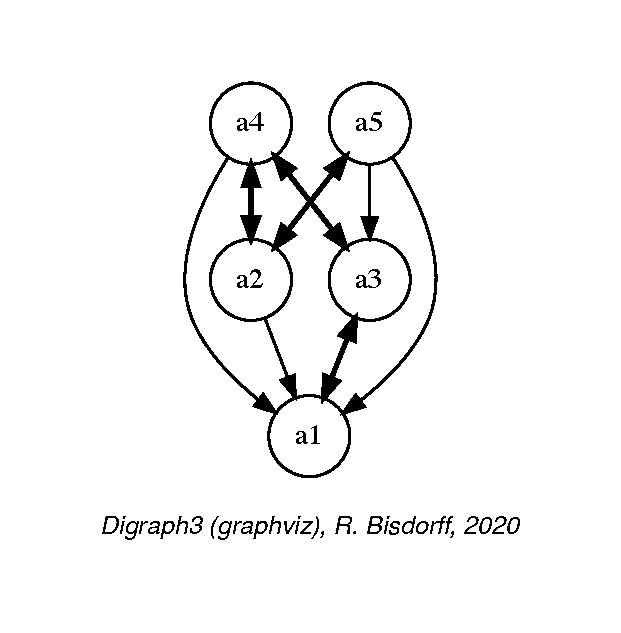
\includegraphics[width=7cm]{Figures/1-1-tutorialDigraph.pdf}
\caption[The tutorial crisp digraph]{The tutorial crisp digraph. The \texttt{exportGraphViz()} method is depending on drawing tools from \texttt{https://graphviz.org}. On Linux Ubuntu or Debian you may try '\texttt{sudo apt-get install graphviz}’ to install them. For Mac OSX There are ready $dmg$ installers available}
\label{fig:1.1}       % Give a unique label
\end{figure}

Further methods are provided for inspecting this random \texttt{Digraph} object \texttt{dg}, like the following \texttt{showStatistics()}\index{showStatistics@\texttt{showStatistics()}} method.
\begin{lstlisting}[caption={Inspecting a \texttt{Digraph} object},label=list:1.5]
>>> dg.showStatistics()
 *----- general statistics -------------*
 for digraph              : <tutorialDigraph.py>
 order                    : 5 nodes
 size                     : 12 arcs
 undetermined           : 0 arcs
 determinateness (%)      : 100.0
 arc density              : 0.60
 double arc density       : 0.40
 single arc density       : 0.40
 absence density          : 0.20
 strict single arc density: 0.40
 strict absence density   : 0.20
 nbr. of components         : 1
 nbr. of strong components  : 1
 transitivity degree (%)  : 60.0
                          : [0, 1, 2, 3, 4, 5]
 outdegrees distribution  : [0, 1, 1, 3, 0, 0]
 indegrees distribution   : [0, 1, 2, 1, 1, 0]
 mean outdegree           : 2.40
 mean indegree            : 2.40
                          : [0, 1, 2, 3, 4, 5, 6, 7, 8, 9, 10]
 symmetric degrees dist.  : [0, 0, 0, 0, 1, 4, 0, 0, 0, 0, 0]
 mean symmetric degree    : 4.80
 outdegrees concentration index   : 0.1667
 indegrees concentration index    : 0.2333
 symdegrees concentration index   : 0.0333
                                  : [0, 1, 2, 3, 4, 'inf']
 neighbourhood depths distribution: [0, 1, 4, 0, 0, 0]
 mean neighbourhood depth         : 1.80
 digraph diameter                 : 2
 agglomeration distribution       :
 a1 : 58.33
 a2 : 33.33
 a3 : 33.33
 a4 : 50.00
 a5 : 50.00
 agglomeration coefficient        : 45.00
\end{lstlisting}

The preceding \texttt{show...()} methods usually rely upon corresponding compute methods, like: \texttt{computeSize()}\index{computeSize@\texttt{computeSize()}}, \texttt{computeDeterminateness()}\index{computeDeterminateness@\texttt{computeDeterminateness()}},\\ or \texttt{computeTransitivityDegree()}\index{computeTransitivityDegree@\texttt{computeTransitivityDegree()}}.
\begin{lstlisting}[caption={Various \texttt{compute...()} methods.},label=list:1.6]
>>> dg.computeSize()
 12
>>> dg.computeDeterminateness(InPercents=True)
 Decimal('100.00')
>>> dg.computeTransitivityDegree(InPercents=True)
 Decimal('60.00')
\end{lstlisting}

Mind that \texttt{show...()} methods output their results in the \emph{Python} console. We provide also some \texttt{showHTML...()} methods which output their results in a system browser’s tab or window.
\begin{lstlisting}
>>> dg.showHTMLRelationMap(relationName='r(x,y)',\
...                        rankingRule=None)
\end{lstlisting}
\begin{figure}[ht]
\sidecaption[t]
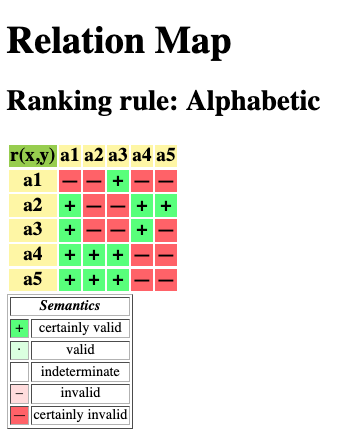
\includegraphics[width=5cm]{Figures/1-2-relationMap1.png}
\caption[Browsing the relation map of the tutorial digraph]{Browsing the relation map of the tutorial digraph. $+$ indicates a certainly valid and $-$ indicates a certainly  invalid relation, Here we find confirmed again that our random digraph instance \texttt{dg}, is indeed a crisp, i.e. $100\%$ determined irreflexive digraph instance}
\label{fig:1.2}       % Give a unique label
\end{figure}

% \section{Special digraph instances}
% \label{sec:1.5}

Some special types of digraph instances, like the \texttt{CirculantDigraph}\index{CirculantDigraph@\texttt{CirculantDigraph} class} or the \texttt{GridDigraph}\index{GridDigraph@\texttt{GridDigraph} class} classes, are readily available (see Fig.~\vref{fig:1.3}).
 \begin{figure}[ht]
%\sidecaption[t]
  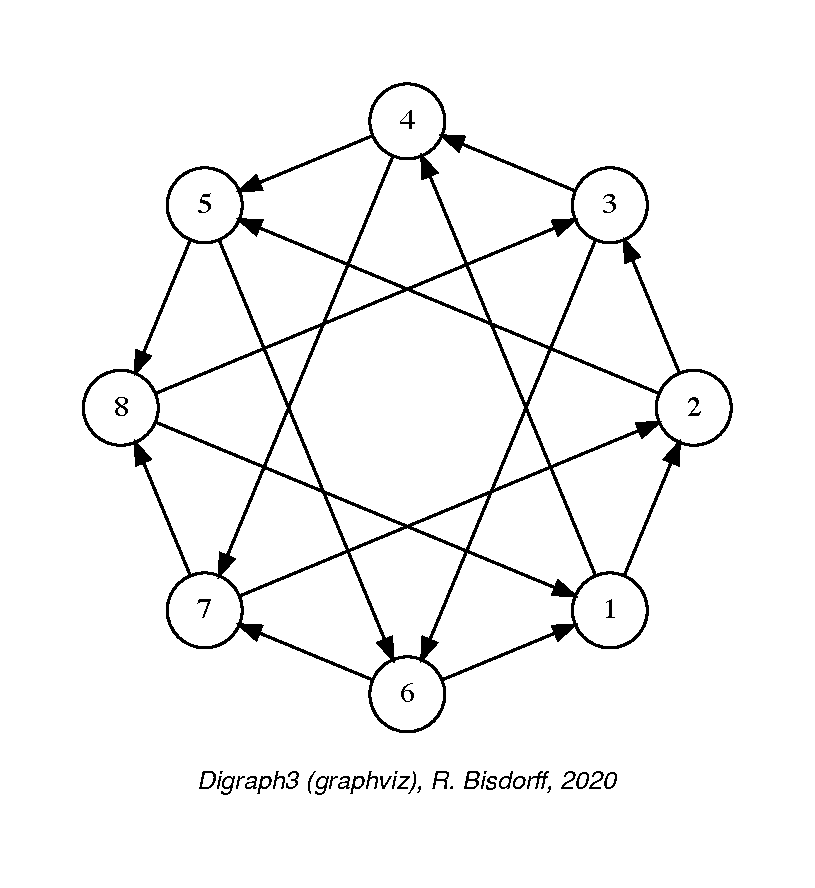
\includegraphics[height=6cm]{Figures/1-3-c8.pdf} \hfill
  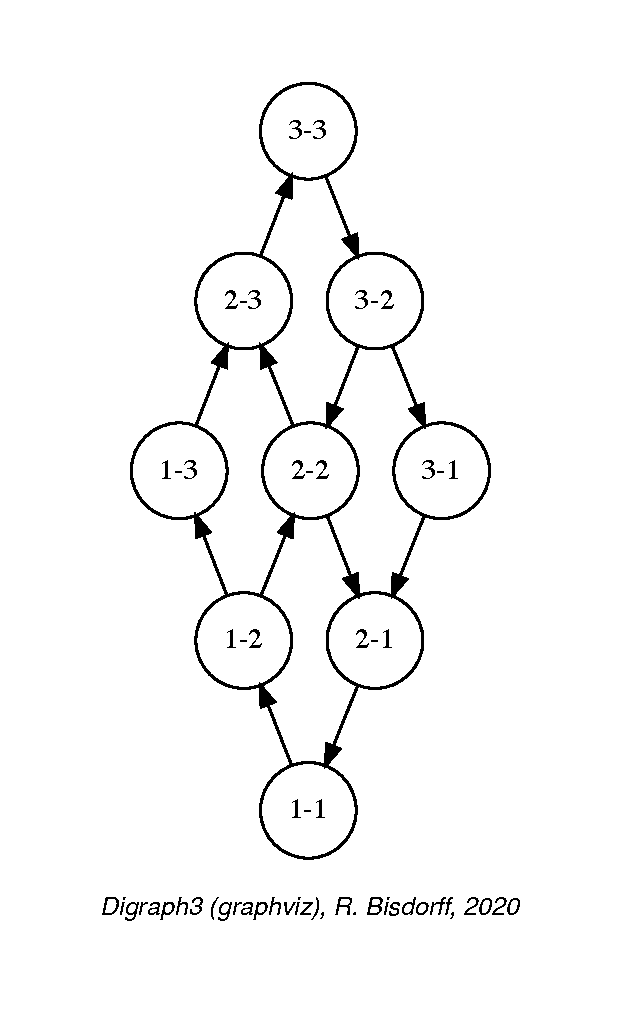
\includegraphics[height=6cm]{Figures/1-3-grid3.pdf} \hfill
  \caption{The circulant [1,3] digraph and the 3x3 grid digraph}
\label{fig:1.3}       % Give a unique label
\end{figure}
\begin{lstlisting}[caption={Circulant digraphs and $n \times m$ grid digraphs},label=list:1.7]
>>> from digraphs import CirculantDigraph,GridDigraph
>>> c8 = CirculantDigraph(order=8,circulants=[1,3])
>>> c8.exportGraphViz('c8')
  *---- exporting a dot file for GraphViz tools ----*
   Exporting to c8.dot
   circo -Tpng c8.dot -o c8.png
>>> grid3 = GridDigraph(n=3,m=3,\
...                    hasMedianSplitOrientation=True)
>>> grid.exportGraphViz('grid3')
  *---- exporting a dot file for GraphViz tools ----*
   Exporting to grid3.dot
   dot -Grankdir=BT -Tpng grid3.dot -o grid3.png
 \end{lstlisting}

%\vspace{1cm}
\vspace{\baselineskip}
The next Chapter~\ref{sec:2} will introduce the fondamental \emph{bipolar-valued digraph} model which is \emph{root object type} to all the digraph models implemented in the \Digraph modules \citep{BIS-2021b}.    

%%%%%%% The chapter bibliography
% % \normallatexbib
%\phantomsection
%\addcontentsline{toc}{section}{Chapter Bibliography}
%\input{02-mainMatters/01-chapterIntroDigraph3.bbl}
\bibliographystyle{spbasic}
\bibliography{03-backMatters/reference}

\bibliographystyle{spbasic}
\bibliography{03-backMatters/reference}

\bibliographystyle{spbasic}
\bibliography{03-backMatters/reference}

\chapter{Working with bipolar-valued digraphs}
\label{sec:2}

\abstract*{ The chapter introduces bipolar-valued digraphs, the fondamental root type of all the specialised digraphs implemented in the \Digraph modules. With the help of a randomly valued digraph, we illustrate some basic digraph manipulation methods, like drawing the digraph, dividing the digraph into its asymmetric and symmetric parts, separating the border from the inner part, computing associated dual, converse and codual digraphs, and operating symmetric and transitive closures.}

\abstract{ The chapter introduces bipolar-valued digraphs, the fondamental root type of all the specialised digraphs implemented in the \Digraph modules. With the help of a randomly valued digraph, we illustrate some basic digraph manipulation methods, like drawing the digraph, dividing the digraph into its asymmetric and symmetric parts, separating the border from the inner part, computing associated dual, converse and codual digraphs, and operating symmetric and transitive closures.}

\section{Random bipolar-valued digraphs}

In Listing~\vref{list:2.1}, we generate a uniformly random $[-1.0; +1.0]$-valued digraph of order 7, denoted \texttt{rdg} and modelling, for instance, a binary relation $S(x,y)$ defined on the set of nodes of \texttt{rdg}. For this purpose, the \Digraph resources provide in the \texttt{randomDigraphs}\index{randomDigraphs@\texttt{randomDigraphs} module} module a specific \texttt{RandomValuationDigraph}\index{RandomValuationDigraph@\texttt{RandomValuationDigraph} class} class \citep{BIS-2021b}.
\begin{lstlisting}[caption={Random bipolar-valued digraph instance},label=list:2.1]
>>> from randomDigraphs import RandomValuationDigraph
>>> rdg = RandomValuationDigraph(order=7)
>>> rdg.save('tutRandValDigraph')
>>> from digraphs import Digraph
>>> rdg = Digraph('tutRandValDigraph')
>>> rdg
  *------- Digraph instance description ------*
   Instance class      : Digraph
   Instance name       : tutRandValDigraph
   Digraph Order       : 7
   Digraph Size        : 22
   Valuation domain    : [-1.00;1.00]
   Determinateness (%) : 75.24
   Attributes          : ['name','actions','order',
                          'valuationdomain','relation',
                          'gamma','notGamma']
\end{lstlisting}   

With the \texttt{save()} \index{save@\texttt{save()}} method (see Line 3) we keep for future use a backup version of \texttt{rdg} which is saved into a file named \texttt{tutRandValDigraph.py} in the current working directory. The genuine \texttt{Digraph} class constructor may restore the \texttt{rdg} object from the stored file (Lines 4-5). We may easily inspect the content of \texttt{rdg} (Line 6). The digraph size 22 indicates the number of positively valued arcs. The valuation domain is uniformly distributed in the interval $[-1.0; 1.0]$ and the mean absolute arc valuation is $(0.7524 \times 2)\, -\, 1.0 \;=\; 0.5048$ (Line 13).

As mentioned in the previous Chapter~\ref{sec:1}, all objects of \texttt{Digraph} type contain at least the list of attributes shown here in Lines 14-16: --a \texttt{name} (string), --a dictionary of \texttt{actions} (digraph nodes), --an \texttt{order} (integer) attribute containing the number of actions, --a \texttt{valuationdomain} dictionary, --a double dictionary \texttt{relation} representing the adjacency table of the digraph relation, --a \texttt{gamma} and --a {\tt notGamma} dictionary containing the direct neighbourhood of each action.

The \texttt{Digraph} class provides some generic \texttt{show...()} methods for exploring the content of a given \texttt{ Digraph} object, like the \texttt{showRelationTable()}\index{showRelationTable@\texttt{showRelationTable()}}, the \texttt{showComponents()}\index{showComponents@\texttt{showComponents()}} and the \texttt{showNeighborhoods()}\index{showNeighborhoods@\texttt{showNeighborhoods()}} methods.
\begin{lstlisting}[caption={Example of random valuation digraph},label=list:2.2]
>>> rdg.showRelationTable()
  * ---- Relation Table -----
   r(xSy) |  '1'    '2'   '3'  '4'   '5'    '6'  '7'	  
   -------|-------------------------------------------
    '1'   |  0.00 -0.48  0.70  0.86  0.30  0.38  0.44	 
    '2'   | -0.22  0.00 -0.38  0.50  0.80 -0.54  0.02	 
    '3'   | -0.42  0.08  0.00  0.70 -0.56  0.84 -1.00	 
    '4'   |  0.44 -0.40 -0.62  0.00  0.04  0.66  0.76	 
    '5'   |  0.32 -0.48 -0.46  0.64  0.00 -0.22 -0.52	 
    '6'   | -0.84  0.00 -0.40 -0.96 -0.18  0.00 -0.22	 
    '7'   |  0.88  0.72  0.82  0.52 -0.84  0.04  0.00
>>> rdg.showComponents()
  *--- Connected Components ---*
  1: ['1', '2', '3', '4', '5', '6', '7']
>>> rdg.showNeighborhoods()
  *---- Neighborhoods ------*
     Gamma:
     '1': in => {'5','7','4'}, out => {'5','7','6','3','4'}
     '2': in => {'7','3'},out => {'5','7','4'}
     '3': in => {'7','1'}, out => {'6','2','4'}
     '4': in => {'5','7','1','2','3'}, out => {'5','7','1','6'}
     '5': in => {'1','2','4'}, out => {'1','4'}
     '6': in => {'7','1','3','4'}, out => set()
     '7': in => {'1','2','4'}, out => {'1','2','3','4','6'}
     Not Gamma:
     '1': in => {'6','2','3'}, out => {'2'}
     '2': in => {'5','1','4'}, out => {'1','6','3'}
     '3': in => {'5','6','2','4'}, out => {'5','7','1'}
     '4': in => {'6'}, out => {'2','3'}
     '5': in => {'7','6','3'}, out => {'7','6','2','3'}
     '6': in => {'5','2'}, out => {'5','7','1','3','4'}
     '7': in => {'5','6','3'}, out => {'5'}
\end{lstlisting}   

Mind that some \texttt{Digraph} class methods will ignore the \emph{reflexive} links by considering that they are \emph{indeterminate}, i.e. the characteristic value $r(x\,S\,x)$ for all action $x$ is set to the \emph{median}, i.e. \emph{indeterminate} value $0.0$ in this case (see Listing~\vref{list:2.2} Lines 5-11 and \citet{BIS-2004a}).

\section{Graphviz drawings}
\label{sec:2.2}

An even better insight into the \texttt{Digraph} object \texttt{rdg} is given by looking at its \href{https://graphviz.org/}{graphviz} drawing \citep{graphviz}\footnote{The \texttt{exportGraphViz()} method is depending on drawing tools from the graphviz software (https://graphviz.org/). On Linux Ubuntu or Debian you may try \texttt{sudo apt-get install graphviz} to install them. There are ready \emph{dmg} installers for Mac OSX.}\index{graphviz}.
\begin{lstlisting}
>>> rdg.exportGraphViz('tutRandValDigraph')
 *---- exporting a dot file for GraphViz tools ------*
  Exporting to tutRandValDigraph.dot
  dot -Grankdir=BT -Tpng tutRandValDigraph.dot\
                           -o tutRandValDigraph.png
\end{lstlisting}
\begin{figure}[ht]
\sidecaption[t]
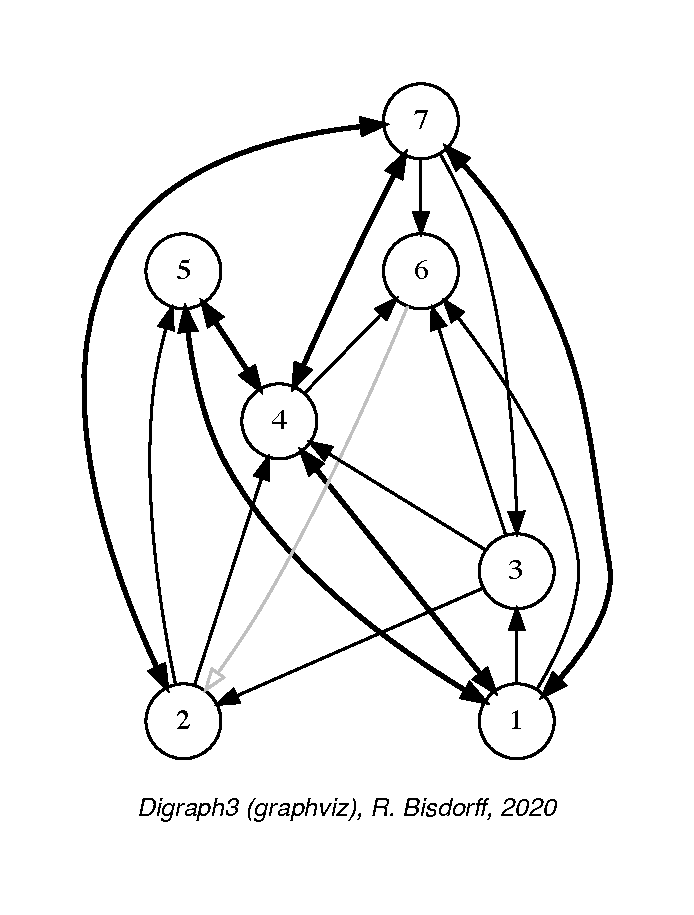
\includegraphics[width=6cm]{Figures/2-1-tutRandValDigraph.pdf}
\caption{\emph{The tutorial random valuation digraph}. Double links are drawn in bold black with an arrowhead at each end, whereas single asymmetric links are drawn in black with an arrowhead showing the direction of the link. Notice the undetermined relational situation ($r(6\,S\,2) = 0.00$) observed between nodes '6' and '2'. The corresponding link is marked in gray with an open arrowhead in the drawing}
\label{fig:2.1}       % Give a unique label
\end{figure}
  
\section{Asymmetric and symmetric parts}
\label{sec:2.3}

We may now extract both the \emph{}\emph{symmetric} as well as the \emph{asymmetric} part of digraph \texttt{rdg} with the help of two corresponding constructors (see List.~\vref{list:2.3}) \index{AsymmetricPartialDigraph@\texttt{AsymmetricPartialDigraph} class}\index{SymmetricPartialDigraph@\texttt{SymmetricPartialDigraph} class}.
\begin{lstlisting}[caption={Computing asymmetric and symmetric Parts},label=list:2.3]
>>> from digraphs import AsymmetricPartialDigraph,\
...                      SymmetricPartialDigraph
>>> asymDg = AsymmetricPartialDigraph(rdg)
>>> asymDg.exportGraphViz()
>>> symDg = SymmetricPartialDigraph(rdg)
>>> symDg.exportGraphViz()
\end{lstlisting}
\begin{figure}[ht]
  % \sidecaption
  Asymmetric Part \hfill Symmetric Part \\
  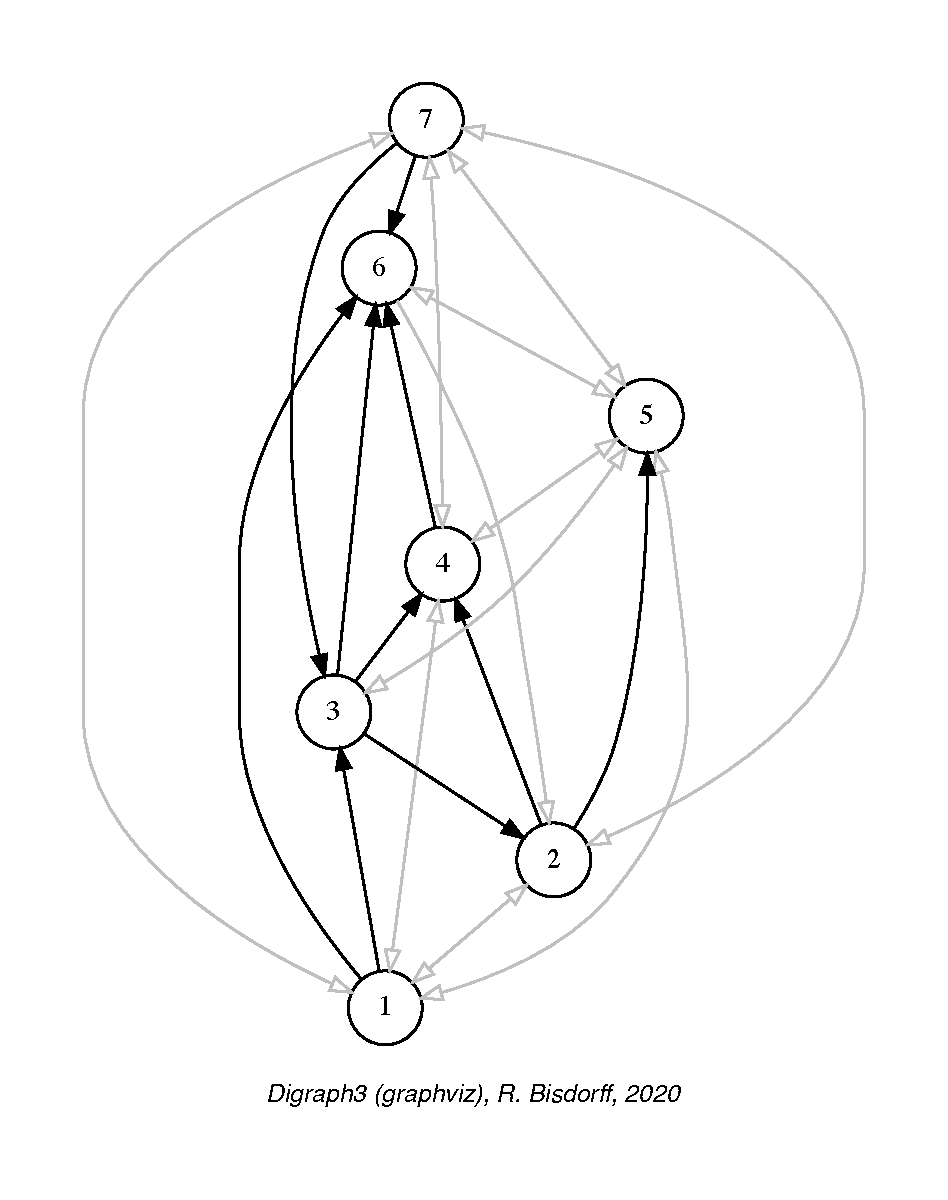
\includegraphics[height=6cm]{Figures/2-2-asymmetricPart.pdf}\hfill
  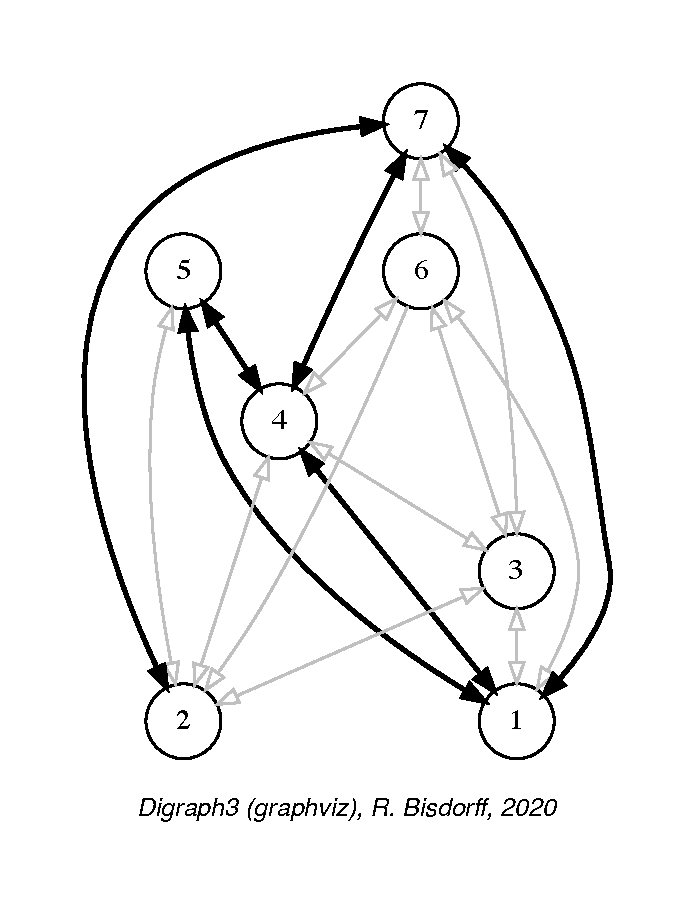
\includegraphics[height=6cm]{Figures/2-2-symmetricPart.pdf}\hfill
\caption{Asymmetric and symmetric part of the tutorial random valuation digraph}
\label{fig:2.2}       % Give a unique label
\end{figure}

The constructor of the partial objects \texttt{asymDg} and \texttt{symDg} puts to the indeterminate characteristic value all non-asymmetric, respectively non-symmetric links between nodes (see Fig.~\vref{fig:2.2}).

Here below, for illustration the source code of the \texttt{ relation} constructor of the \texttt{AsymmetricPartialDigraph} class.
\begin{lstlisting}[caption={Computing the asymmetric part of a bipolar-valued relation},label=list:2.4,basicstyle=\ttfamily\scriptsize]
def _constructRelation(self):
    actions = self.actions
    Min = self.valuationdomain['min']
    Max = self.valuationdomain['max']
    Med = self.valuationdomain['med']
    relationIn = self.relation
    relationOut = {}
    for a in actions:
	relationOut[a] = {}
	for b in actions:
	    if a != b:
                if relationIn[a][b] >= Med and relationIn[b][a] <= Med:
		    relationOut[a][b] = relationIn[a][b]
		elif relationIn[a][b] <= Med and relationIn[b][a] >= Med:
		    relationOut[a][b] = relationIn[a][b]
		else:
		    relationOut[a][b] = Med
	    else: # reflexive links are ignored
		relationOut[a][b] = Med
    return relationOut
\end{lstlisting}

\section{Border and inner parts}
\label{sec:2.4}

We may also extract the \emph{border} --the part of a digraph induced by the union of its initial and terminal prekernels (see Chap.~\ref{sec:17})--  as well as, the \emph{inner part} --the complement of the border-- with the help of two corresponding class constructors: \texttt{GraphBorder}\index{GraphBorder@\texttt{GraphBorder} class} and \texttt{GraphInner}\index{GraphInner@\texttt{GraphInner} class} (see Fig.~\vref{fig:2.3}).

\begin{figure}[ht]
%\sidecaption
  Border Part \hfill Inner Part \\
  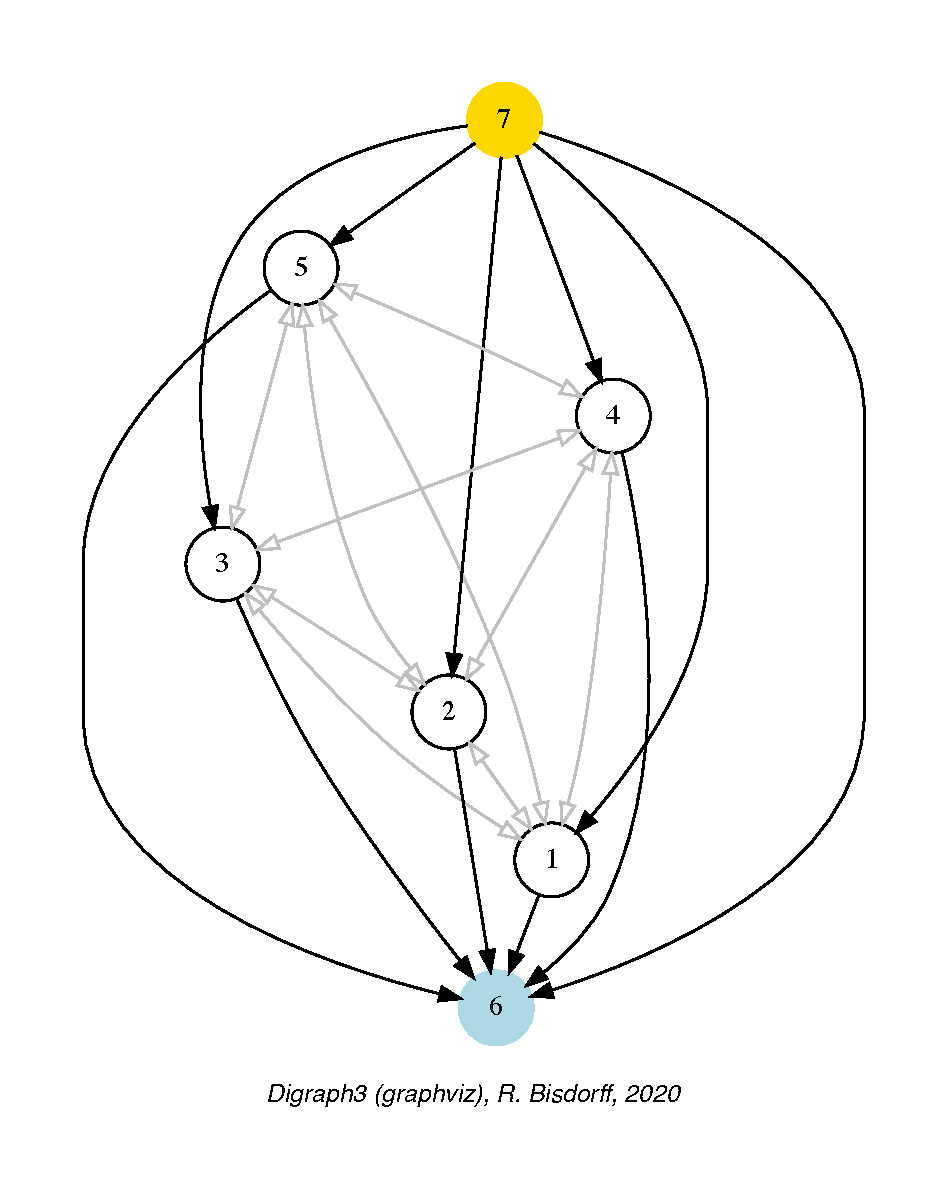
\includegraphics[height=6cm]{Figures/2-3-linearOrderBorder.pdf}\hfill
  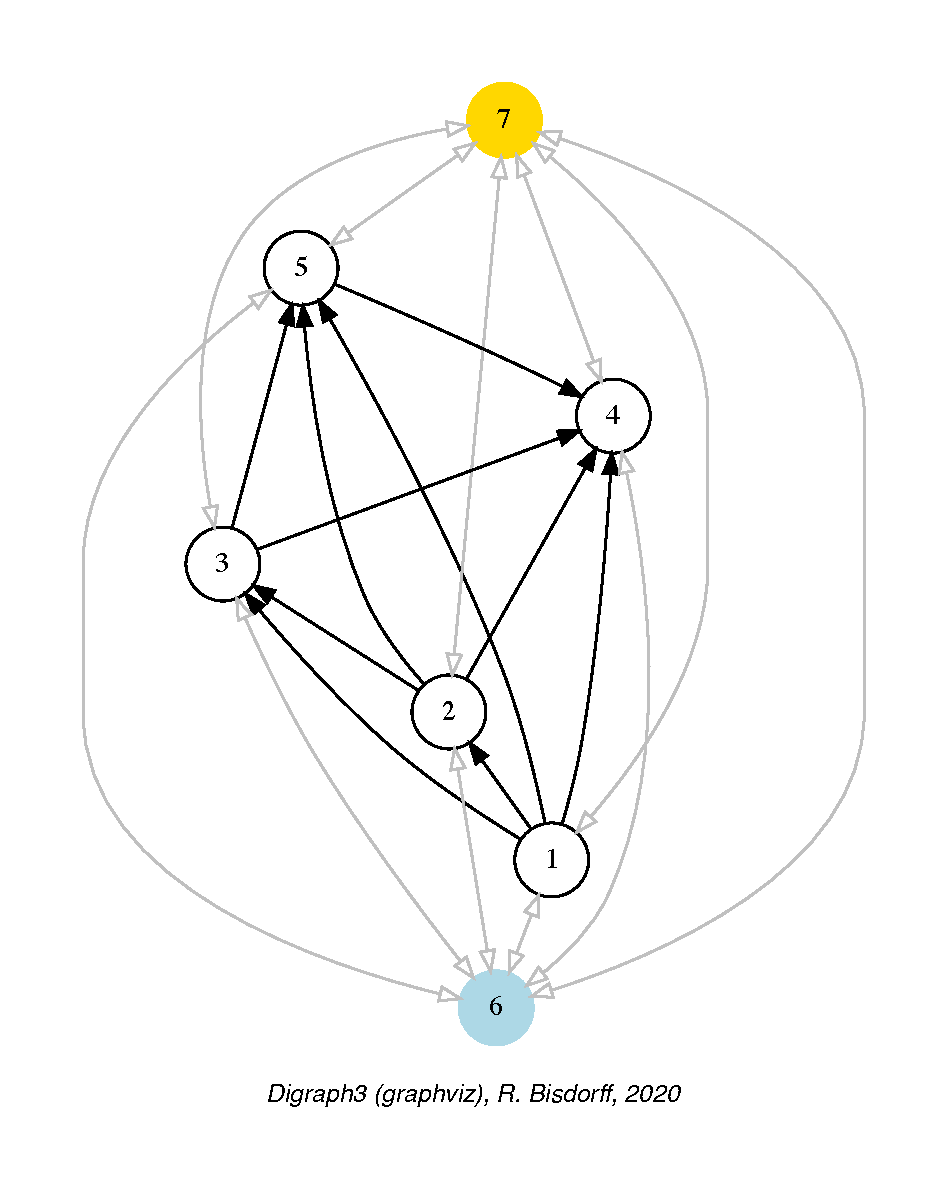
\includegraphics[height=6cm]{Figures/2-3-linearOrderInner.pdf}\hfill
\caption{\emph{Border} and \emph{inner} part of a linear order oriented by \emph{terminal} and \emph{initial} kernels.}
\label{fig:2.3}       % Give a unique label
\end{figure}
Let us illustrate the digraph border and inner parts on a linear ordering obtained from the tutorial random valuation digraph \texttt{rdg}  with the \NetFlows ranking rule  (see Sec.~\ref{sec:8.3}).  
\begin{lstlisting}[caption={Border and inner part of a linear order},label=list:2.5]
>>> from digraphs import GraphBorder, GraphInner
>>> from linearOrders import NetFlowsOrder
>>> nf = NetFlowsOrder(rdg)
>>> nf.netFlowsOrder
   ['6', '4', '5', '3', '2', '1', '7']
>>> bnf = GraphBorder(nf)
>>> bnf.exportGraphViz(lastChoice=['6'],firstChoice=['7'])
>>> inf = GraphInner(nf)
>>> inf.exportGraphViz(lastChoice=['6'],firstChoice=['7'])
\end{lstlisting}
We may orient the \texttt{graphviz} drawings in Figure~\vref{fig:2.3}  with the terminal node 6 (\texttt{lastChoice} parameter) and initial node 7 (\texttt{firstChoice} parameter) (see List.~\vref{list:2.5} Lines 7 and 9).

The constructor of the partial digraphs \texttt{bnf} and \texttt{inf}  (see Lines 3 and 6) puts to the \emph{indeterminate} characteristic value all links not in the \emph{border}, respectively \emph{not} in the \emph{inner} part (see Fig.~\vref{fig:2.3}). Being much {\em denser\/} than a linear order, the actual inner part of our tutorial random valuation digraph \texttt{rdg} is reduced to a single arc between nodes 3 and 4 (see Fig.~\vref{fig:2.4}). Indeed, a complete digraph on the limit has no inner part (privacy!) at all, whereas empty and indeterminate digraphs admit both, an empty border and an empty inner part.
\begin{figure}[h]
%\sidecaption
  Border Part \hfill Inner Part \\
  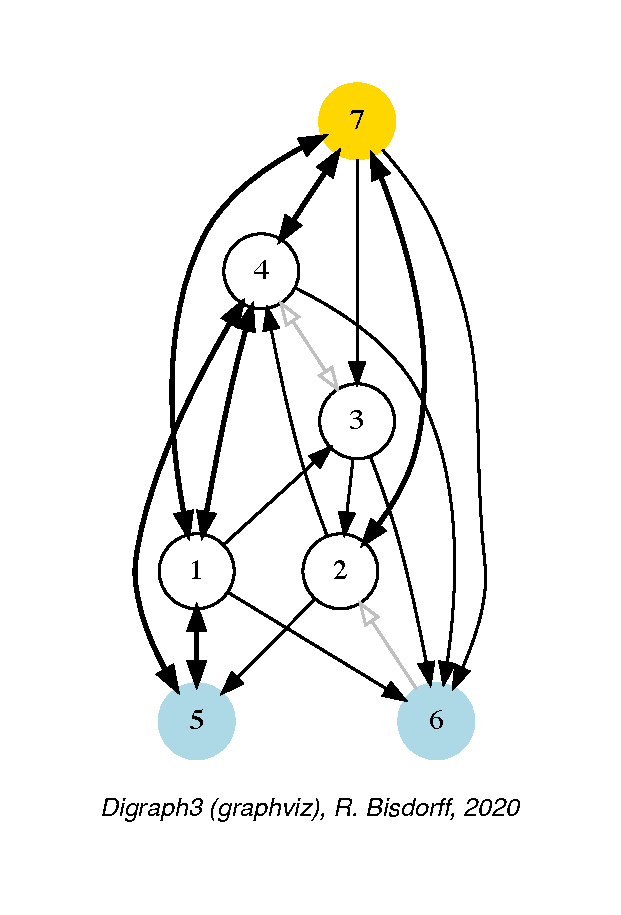
\includegraphics[height=6cm]{Figures/2-4-tutRandValDigraph_border.pdf}\hfill
  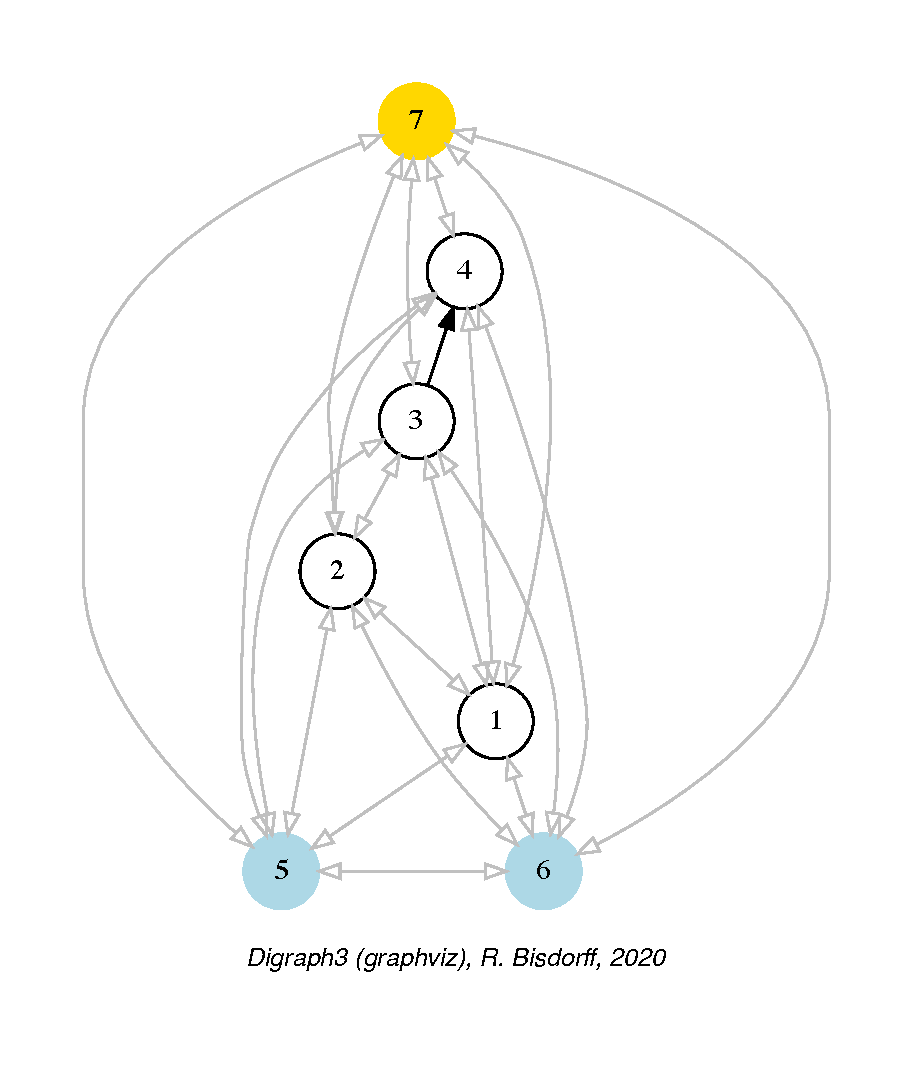
\includegraphics[height=6cm]{Figures/2-4-tutRandValDigraph_inner.pdf}\hfill
\caption{Border and inner part of the tutorial random valuation digraph \texttt{rdg}}
\label{fig:2.4}       % Give a unique label
\end{figure}

\section{Fusion by epistemic disjunction}
\label{sec:2.5}

We may recover object \texttt{rdg} from both partial objects \texttt{asymDg} and \texttt{symDg}, or as well from the border \texttt{bg} and the inner part \texttt{ig}, with a \emph{bipolar fusion} operator, also called \emph{epistemic disjunction}, available via the \texttt{FusionDigraph}\index{FusionDigraph@\texttt{FusionDigraph} class} class. 
\begin{lstlisting}[caption={Epistemic fusion of partial diagraphs},label=list:2.6]
>>> from digraphs import FusionDigraph
>>> fusDg = FusionDigraph(asymDg,symDg,operator='o-max')
>>> # fusDg = FusionDigraph(bg,ig,operator='o-max')
>>> fusDg.showRelationTable()
  * ---- Relation Table -----
   r(xSy) |  '1'    '2'   '3'  '4'   '5'    '6'  '7'	  
   -------|------------------------------------------
    '1'   |  0.00 -0.48  0.70  0.86  0.30  0.38  0.44	 
    '2'   | -0.22  0.00 -0.38  0.50  0.80 -0.54  0.02	 
    '3'   | -0.42  0.08  0.00  0.70 -0.56  0.84 -1.00	 
    '4'   |  0.44 -0.40 -0.62  0.00  0.04  0.66  0.76	 
    '5'   |  0.32 -0.48 -0.46  0.64  0.00 -0.22 -0.52	 
    '6'   | -0.84  0.00 -0.40 -0.96 -0.18  0.00 -0.22	 
    '7'   |  0.88  0.72  0.82  0.52 -0.84  0.04  0.00
\end{lstlisting}

The epistemic fusion operator \texttt{o-max} (see List.~\vref{list:2.6} Line 2) is defined as follows:
\begin{definition}[Disjunctive epistemic fusion operator \texttt{o-max}]\label{def:disjunctiveFusion}

\noindent Let $r$ and $r'$ characterise two bipolar-valued epistemic situations:
\begin{itemize}[leftmargin=0.5cm,rightmargin=0.5cm,nosep]
\item \texttt{o-max}$(r, r')$ = $\max(r, r' )$ when both $r$ and $r'$ are more or less valid or indeterminate;
\item \texttt{o-max}$(r, r')$ = $\min(r, r' )$ when both $r$ and $r'$ are more or less invalid or indeterminate;
\item \texttt{o-max}$(r, r')$ = $0.0$, i.e. indeterminate otherwise.
\end{itemize}
\end{definition}

Mind that the \texttt{o-max} operator, like a mean operator, is \emph{not associative} when more than 2 operands are given. In order to make the \texttt{o-max} fusion univocal, the following rule is applied: --first, all positive and negative terms are separately aggregated, --then the \texttt{o-max} fusion is applied on both aggregates.

\section{Dual, converse and codual digraphs}
\label{sec:2.6}

We may as readily compute the \emph{dual}\index{DualDigraph@\texttt{DualDigraph} class} (negated relation \footnote{Not to be confused with the dual graph of a plane graph $g$ that has a vertex for each face of $g$. Here we mean the \emph{less than} (strict converse) relation corresponding to a \emph{greater or equal} relation, or the \emph{less than or equal} relation corresponding to a (strict) \emph{better than} relation.}), the \emph{converse}\index{ConverseDigraph@\texttt{ConverseDigraph} class} (transposed relation) and the \emph{codual}\index{CoDualDigraph@\texttt{CoDualDigraph} class} (transposed and negated relation) of the digraph instance \texttt{rdg}. 
\begin{lstlisting}[caption={Computing associated dual, converse and codual digraphs},label=list:2.7]
>>> from digraphs import\
...          DualDigraph, ConverseDigraph, CoDualDigraph
>>> # dual of rdg
>>> ddg = DualDigraph(rdg)
>>> ddg.showRelationTable()
    -r(xSy) |  '1'    '2'   '3'  '4'   '5'    '6'  '7'	  
    --------|------------------------------------------
    '1 '    |  0.00  0.48 -0.70 -0.86 -0.30 -0.38 -0.44	 
    '2'     |  0.22  0.00  0.38 -0.50  0.80  0.54 -0.02	 
    '3'     |  0.42  0.08  0.00 -0.70  0.56 -0.84  1.00	 
    '4'     | -0.44  0.40  0.62  0.00 -0.04 -0.66 -0.76	 
    '5'     | -0.32  0.48  0.46 -0.64  0.00  0.22  0.52	 
    '6'     |  0.84  0.00  0.40  0.96  0.18  0.00  0.22	 
    '7'     |  0.88 -0.72 -0.82 -0.52  0.84 -0.04  0.00
>>> # converse of rdg
>>> cdg = ConverseDigraph(rdg)
>>> cdg.showRelationTable()
    * ---- Relation Table -----
     r(ySx) |  '1'    '2'   '3'   '4'   '5'   '6'   '7'	  
    --------|------------------------------------------
    '1'     |  0.00 -0.22 -0.42  0.44  0.32 -0.84  0.88	 
    '2'     | -0.48  0.00  0.08 -0.40 -0.48  0.00  0.72	 
    '3'     |  0.70 -0.38  0.00 -0.62 -0.46 -0.40  0.82	 
    '4'     |  0.86  0.50  0.70  0.00  0.64 -0.96  0.52	 
    '5'     |  0.30  0.80 -0.56  0.04  0.00 -0.18 -0.84	 
    '6'     |  0.38 -0.54  0.84  0.66 -0.22  0.00  0.04	 
    '7'     |  0.44  0.02 -1.00  0.76 -0.52 -0.22  0.00	 
>>> # codual of rdg
>>> cddg = CoDualDigraph(rdg)
>>> cddg.showRelationTable()
    * ---- Relation Table -----
    -r(ySx) |  '1'    '2'   '3'   '4'   '5'   '6'   '7'	    
    --------|------------------------------------------
    '1'     |  0.00  0.22  0.42 -0.44 -0.32  0.84 -0.88	 
    '2'     |  0.48  0.00 -0.08  0.40  0.48  0.00 -0.72	 
    '3'     | -0.70  0.38  0.00  0.62  0.46  0.40 -0.82	 
    '4'     | -0.86 -0.50 -0.70  0.00 -0.64  0.96 -0.52	 
    '5'     | -0.30 -0.80  0.56 -0.04  0.00  0.18  0.84	 
    '6'     | -0.38  0.54 -0.84 -0.66  0.22  0.00 -0.04	 
    '7'     | -0.44 -0.02  1.00 -0.76  0.52  0.22  0.00	 
\end{lstlisting}

Computing the \emph{dual}, respectively the \emph{converse} of a digraph, may also be done with prefixing the \texttt{\_\_neg\_\_} ($-$) or the \texttt{\_\_invert\_\_} ($\sim$) operator. The \emph{codual} of a \texttt{Digraph} object may, hence, as well be computed with a \emph{composition} (in either order) of both operations.
\begin{lstlisting}[caption={Computing the dual, the converse and the codual of a digraph},label=list:2.8]
>>> ddg = -rdg   # dual of rdg
>>> cdg = ~rdg   # converse of rdg
>>> cddg = ~(-rdg) # = -(~(rdg) codual of rdg
>>> (-(~rdg)).showRelationTable()
  * ---- Relation Table -----
   -r(ySx) |  '1'    '2'   '3'   '4'   '5'   '6'   '7'	    
   --------|------------------------------------------
   '1'     |  0.00  0.22  0.42 -0.44 -0.32  0.84 -0.88	 
   '2'     |  0.48  0.00 -0.08  0.40  0.48  0.00 -0.72	 
   '3'     | -0.70  0.38  0.00  0.62  0.46  0.40 -0.82	 
   '4'     | -0.86 -0.50 -0.70  0.00 -0.64  0.96 -0.52	 
   '5'     | -0.30 -0.80  0.56 -0.04  0.00  0.18  0.84	 
   '6'     | -0.38  0.54 -0.84 -0.66  0.22  0.00 -0.04	 
   '7'     | -0.44 -0.02  1.00 -0.76  0.52  0.22  0.00	 
\end{lstlisting}
  
\section{Symmetric and transitive closures}
\label{sec:2.7}

Symmetric and transitive closures, by default in-site methods, are also available (see Fig.~\vref{fig:2.5})\index{closeSymmetric@\texttt{closeSymmetric()}}\index{closeTransitive@\texttt{closeTransitive()}}. Note that it is a good idea, before going ahead with these in-site operations, who irreversibly modify the original \texttt{rdg} object, to previously make a backup version of \texttt{rdg}. The simplest storage method, always provided by the generic \texttt{Digraph.save()} method, writes out in a named file the python content of the Digraph object in string representation (see Sec.~\vref{sec:1.3}).
\begin{lstlisting}[caption={Symmeric and transitive closures},label=list:2.9]
>>> rdg.save('tutRandValDigraph')
>>> rdg.closeSymmetric(InSite=True)
>>> rdg.closeTransitive(InSite=True)
>>> rdg.exportGraphViz('strongComponents')
\end{lstlisting}
\begin{figure}[h]
\sidecaption[t]
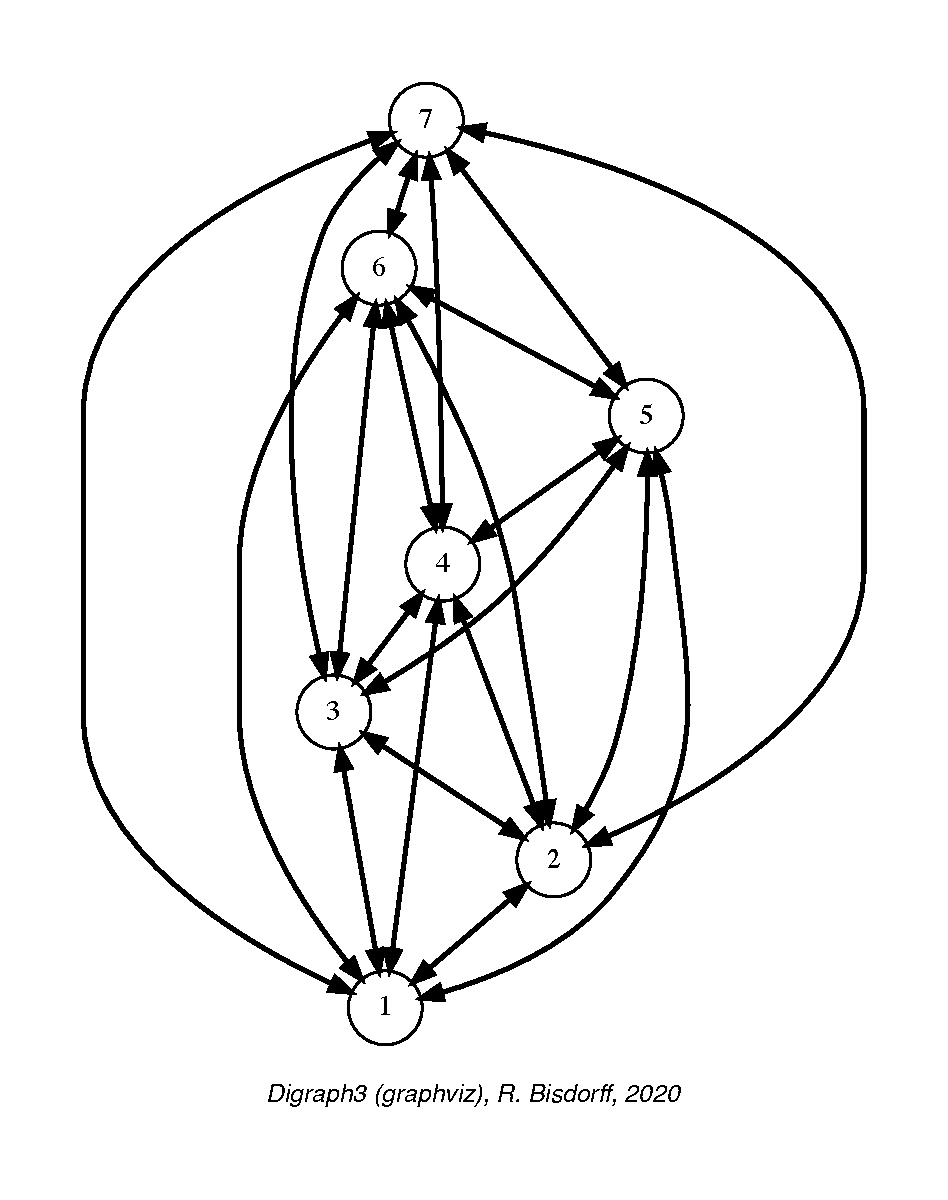
\includegraphics[width=6cm]{Figures/2-5-strongComponents.pdf}
\caption{Symmetric and transitive closure of the tutorial random valuation digraph $rdg$.}
\label{fig:2.5}       % Give a unique label
\end{figure}

The \texttt{closeSymmetric()}\index{closeSymmetric@\texttt{closeSymmetric()}} method (see List.~\vref{list:2.9} Line 2), of complexity $O(n^2)$ where $n$ denotes the digraph's order, changes, on the one hand, all single pairwise links it may detect into double links by operating a disjunction of the pairwise relations. On the other hand, the \texttt{closeTransitive()}\index{closeTransitive@\texttt{closeTransitive()}}  method (see Line 3), implements the \emph{Roy-Warshall} transitive closure algorithm of complexity $O(n^3)$ \index{Roy@\textsl{B. Roy}} \index{warshall@\textsl{S. Warshall}} (\citealp{ROY-1959} and \citealp{WAR-1962}).

The same \texttt{closeTransitive()} with a \texttt{Reverse = True} flag may be readily used for eliminating all transitive arcs from a transitive digraph instance. We make usage of this feature when drawing Hasse diagrams of \texttt{TransitiveDigraph}\index{TransitiveDigraph@\texttt{TransitiveDigraph} class} objects.

\section{Strong components}
\label{sec:2.8}

As the original digraph \texttt{rdg} was connected (see above the result of the showShort() command), both the symmetric and the transitive closures operated together, will necessarily produce a single strong component, i.e. a \textbf{complete} digraph. We may sometimes wish to collapse all strong components in a given digraph and construct the so \emph{collapsed} digraph. Using the \texttt{StrongComponentsCollapsedDigraph} constructor \index{StrongComponentsCollapsedDigraph@\texttt{StrongComponentsCollapsedDigraph} class} here will render a single hyper-node gathering all the original nodes (see Line 7 below).
\begin{lstlisting}[caption={Computing the strong components in a digraph},label=list:2.10]
>>> from digraphs import StrongComponentsCollapsedDigraph
>>> sc = StrongComponentsCollapsedDigraph(rdg)
>>> sc.showAll()
  *----- show detail -----*
   Digraph          : tutRandValDigraph_Scc
  *---- Actions ----*
    ['_7_1_2_6_5_3_4_']
  *---- Relation Table -----
      S     |  'Scc_1'	  
     -------|---------
     'Scc_1' |  0.00
  *---- strong Components ----*
   short 	 content
   'Scc_1' 	 '_7_1_2_6_5_3_4_'
  *---- Neighborhoods ----*
   Gamma     :
   'frozenset({'7','1','2','6','5','3','4'})':
                     in => set(), out => set()
   Not Gamma :
   'frozenset({'7','1','2','6','5','3','4'})':
                     in => set(), out => set()
\end{lstlisting}
  
\section{CSV storage}
\label{sec:2.9}

Sometimes it is required to exchange the graph valuation data in CSV format with a statistical package like \textbf{R}\footnote{\url{https://www.r-project.org/}}. For this purpose it is possible to export the digraph data into a CSV file. The valuation domain is hereby normalised by default to the range $[-1.0,1.0]$ and the diagonal is put by default to the minimal value $-1.0$.
\begin{lstlisting}
>>> rdg = Digraph('tutRandValDigraph')
>>> rdg.saveCSV('tutRandValDigraph')
  # content of file tutRandValDigraph.csv
  "d","1","2","3","4","5","6","7"
  "1",-1.0,0.48,-0.7,-0.86,-0.3,-0.38,-0.44
  "2",0.22,-1.0,0.38,-0.5,-0.8,0.54,-0.02
  "3",0.42,-0.08,-1.0,-0.7,0.56,-0.84,1.0
  "4",-0.44,0.4,0.62,-1.0,-0.04,-0.66,-0.76
  "5",-0.32,0.48,0.46,-0.64,-1.0,0.22,0.52
  "6",0.84,0.0,0.4,0.96,0.18,-1.0,0.22
  "7",-0.88,-0.72,-0.82,-0.52,0.84,-0.04,-1.0
\end{lstlisting}
  
It is possible to reload a \texttt{Digraph} instance from its previously saved CSV file content.
\begin{lstlisting} 
>>> from digraphs import CSVDigraph   
>>> rdgcsv = CSVDigraph('tutRandValDigraph')
>>> rdgcsv.showRelationTable(ReflexiveTerms=False)
    * ---- Relation Table -----
    r(xSy) |   '1'   '2'   '3'   '4'   '5'   '6'   '7'	  
    -------|------------------------------------------------------------
    '1'    |   -   -0.48  0.70  0.86  0.30  0.38  0.44	 
    '2'    | -0.22   -   -0.38  0.50  0.80 -0.54  0.02	 
    '3'    | -0.42  0.08   -    0.70 -0.56  0.84 -1.00	 
    '4'    |  0.44 -0.40 -0.62   -    0.04  0.66  0.76	 
    '5'    |  0.32 -0.48 -0.46  0.64   -   -0.22 -0.52	 
    '6'    | -0.84  0.00 -0.40 -0.96 -0.18   -   -0.22	 
    '7'    |  0.88  0.72  0.82  0.52 -0.84  0.04   -
\end{lstlisting}
  
It is as well possible to show a coloured version of the valued relation table in a system browser window tab (see Fig.~\vref{fig:2.5}).
\begin{lstlisting}
>>> rdgcsv.showHTMLRelationTable(tableTitle="Tutorial random digraph")
\end{lstlisting}
 \begin{figure}[ht]
\sidecaption[t]
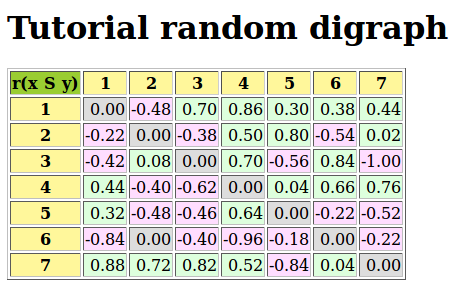
\includegraphics[width=7cm]{Figures/2-6-htmlTutorialDigraph.png}
\caption{The valued relation table shown in a browser window. Positive arcs are shown in green and negative arcs in red. Indeterminate --zero-valued-- links, like the reflexive diagonal ones or the link between node \texttt{'6'} and node \texttt{'2'}, are shown in gray}
\label{fig:2.6}       % Give a unique label
\end{figure}
 
\section{Complete, empty and indeterminate digraphs}
\label{sec:2.10}

Let us finally mention some special universal classes of digraphs that are readily available in the \texttt{digraphs} module\footnote{See \citealp{BIS-2021}}, like:
\begin{itemize}[nosep]
\item the \texttt{CompleteDigraph}\index{CompleteDigraph@\texttt{CompleteDigraph} class},
\item  the \texttt{EmptyDigraph}\index{EmptyDigraph@\texttt{EmptyDigraph} class} and
\item  the \texttt{IndeterminateDigraph}\index{IndeterminateDigraph@\texttt{IndeterminateDigraph} class} class,
\end{itemize}
who put all characteristic values respectively to the \emph{maximum}, the \emph{minimum} or the \emph{median} indeterminate characteristic value.
\begin{lstlisting}[caption={Complete, empty and indeterminate digraphs},label=list:2.11]
>>> from digraphs import CompleteDigraph,EmptyDigraph,\
...   			 IndeterminateDigraph
>>> # the empty digraph   
>>> e = EmptyDigraph(order=5)
>>> e.showRelationTable()
    * ---- Relation Table -----
      S   |    '1'    '2'    '3'    '4'	   '5'	  
    ---- -|-----------------------------------
    '1'   |  -1.00  -1.00  -1.00  -1.00	 -1.00	 
    '2'   |  -1.00  -1.00  -1.00  -1.00	 -1.00	 
    '3'   |  -1.00  -1.00  -1.00  -1.00	 -1.00	 
    '4'   |  -1.00  -1.00  -1.00  -1.00	 -1.00	 
    '5'   |  -1.00  -1.00  -1.00  -1.00	 -1.00
>>> e.showNeighborhoods() 
    Neighborhoods:
      Gamma     :
    '1': in => set(), out => set()
    '2': in => set(), out => set()
    '5': in => set(), out => set()
    '3': in => set(), out => set()
    '4': in => set(), out => set()
      Not Gamma :
    '1': in => {'2','4','5','3'}, out => {'2','4','5','3'}
    '2': in => {'1','4','5','3'}, out => {'1','4','5','3'}
    '5': in => {'1','2','4','3'}, out => {'1','2','4','3'}
    '3': in => {'1','2','4','5'}, out => {'1','2','4','5'}
    '4': in => {'1','2','5','3'}, out => {'1','2','5','3'}
>>> # the indeterminate digraph
>>> i = IndeterminateDigraph()
    * ---- Relation Table -----
      S   |   '1'   '2'	  '3'	'4'   '5'	  
    ------|------------------------------
    '1'   |  0.00  0.00	 0.00  0.00  0.00	 
    '2'   |  0.00  0.00	 0.00  0.00  0.00	 
    '3'   |  0.00  0.00	 0.00  0.00  0.00	 
    '4'   |  0.00  0.00	 0.00  0.00  0.00	 
    '5'   |  0.00  0.00	 0.00  0.00  0.00	 
>>> i.showNeighborhoods()
    Neighborhoods:
      Gamma     :
    '1': in => set(), out => set()
    '2': in => set(), out => set()
    '5': in => set(), out => set()
    '3': in => set(), out => set()
    '4': in => set(), out => set()
      Not Gamma :
    '1': in => set(), out => set()
    '2': in => set(), out => set()
    '5': in => set(), out => set()
    '3': in => set(), out => set()
    '4': in => set(), out => set()
\end{lstlisting}

Mind the subtle difference between the neighbourhoods of an \emph{empty} and the neighbourhoods of an \emph{indeterminate} digraph instance. In the first kind, the neighbourhoods are known to be completely \emph{empty}  (see List.~\vref{list:2.11} Lines 22-27) whereas, in the latter, \emph{nothing is known} about the actual neighbourhoods of the nodes  (see Lines 46-51). These two cases illustrate why in the case of \emph{bipolar-valued} digraphs, we may sometimes need both a \texttt{gamma} \textbf{and} a \texttt{notGamma} attribute.

\vspace{1cm}
In the following Chapter~\ref{sec:3}  we introduce the main formal object of this book, namely \emph{bipolar-valued outranking} digraphs.

%%%%%%%%%%%%%%%%%%%%%%%%%%%%%%%%%%%%
\phantomsection
\addcontentsline{toc}{section}{Notes}
\section*{Notes}

It is \emph{D. Bouyssou} \index{Bouyssou@\emph{D. Bouyssou}} who first suggested us end of the nineties, when we started to work in Prolog on the computation of digraph kernels with finite domain constraint solvers, that the $50\%$ criteria significance majority was a special value to be carefully taken into account. The converging solution vectors of the fixpoint kernel equations confirmed this special status of the $50\%$ majority (see Chap.~\ref{sec:17}). These early insights led to the seminal articles on bipolar-valued epistemic logic where we introduced split truth/falseness semantics for a multi-valued logical processing of fuzzy preference modelling \citep{BIS-2000,BIS-2002}. The characteristic valuation domain remained however the classical fuzzy $[0.0;1.0]$ valuation domain.

It is only in 2004, when we succeeded in assessing the stability of the outranking digraph when solely ordinal criteria significance weights are given, that it became clear and evident for us that the characteristic valuation domain had to be shifted to a bipolar $[-1.0;+1.0]$-valued domain \citep{BIS-2004a}. In this bipolar valuation domain, the $50\%$ majority thershold corresponds now to the median $0.0$ value, characterising with the correct zero value an epistemic indetermination --no knowledge-- situation. Furthermore, identifying truth and falseness by the sign of the characteristic values revealed itself to be very efficient not only from a computational point of view, but also from scientific and semiotical perspectives. A positive (resp. negative) characteristic value now attest a logically valid (resp. invalid) statement and a negative affirmation now corresponds to a positive refutation. Furthermore, the median zero value gives way to efficiently handling partial digraphs --like the border or the assymetric part of a digraph-- and, even more important from a practical decision making point of view, any missing data.

The bipolar $[-1.0;+1.0]$-valued characteritisc domain opened so the way to important new operations and concepts, like the disjunctive epistemic fusion operation seen in Section~\vref{sec:2.5} that confers the outranking digraph a logically and epistemically sound definition \citep{BIS-2013}. \Kendall 's ordinal correlation index could be extended to a bipolar-valued relational equivalence index between digraphs \citep{BIS-2012a}. Making usage of the bipolar-valued Gaussian error function naturally led to defining a bipolar-valued likelihood function, where a positive (resp. negative) value gives the likelihood of an affirmation (resp. a refutation) \citep{BIS-2014}.      

%%%%%%% The chapter bibliography
%\normallatexbib
%\clearpage
%\phantomsection
%\addcontentsline{toc}{section}{Chapter Bibliograhy}
\bibliographystyle{spbasic}
%\typeout{}
\bibliography{03-backMatters/reference}
%\chapter{Working with bipolar-valued digraphs}
\label{sec:2}

\abstract*{ The chapter introduces bipolar-valued digraphs, the fondamental root type of all the specialised digraphs implemented in the \Digraph modules. With the help of a randomly valued digraph, we illustrate some basic digraph manipulation methods, like drawing the digraph, dividing the digraph into its asymmetric and symmetric parts, separating the border from the inner part, computing associated dual, converse and codual digraphs, and operating symmetric and transitive closures.}

\abstract{ The chapter introduces bipolar-valued digraphs, the fondamental root type of all the specialised digraphs implemented in the \Digraph modules. With the help of a randomly valued digraph, we illustrate some basic digraph manipulation methods, like drawing the digraph, dividing the digraph into its asymmetric and symmetric parts, separating the border from the inner part, computing associated dual, converse and codual digraphs, and operating symmetric and transitive closures.}

\section{Random bipolar-valued digraphs}

In Listing~\vref{list:2.1}, we generate a uniformly random $[-1.0; +1.0]$-valued digraph of order 7, denoted \texttt{rdg} and modelling, for instance, a binary relation $S(x,y)$ defined on the set of nodes of \texttt{rdg}. For this purpose, the \Digraph resources provide in the \texttt{randomDigraphs}\index{randomDigraphs@\texttt{randomDigraphs} module} module a specific \texttt{RandomValuationDigraph}\index{RandomValuationDigraph@\texttt{RandomValuationDigraph} class} class \citep{BIS-2021b}.
\begin{lstlisting}[caption={Random bipolar-valued digraph instance},label=list:2.1]
>>> from randomDigraphs import RandomValuationDigraph
>>> rdg = RandomValuationDigraph(order=7)
>>> rdg.save('tutRandValDigraph')
>>> from digraphs import Digraph
>>> rdg = Digraph('tutRandValDigraph')
>>> rdg
  *------- Digraph instance description ------*
   Instance class      : Digraph
   Instance name       : tutRandValDigraph
   Digraph Order       : 7
   Digraph Size        : 22
   Valuation domain    : [-1.00;1.00]
   Determinateness (%) : 75.24
   Attributes          : ['name','actions','order',
                          'valuationdomain','relation',
                          'gamma','notGamma']
\end{lstlisting}   

With the \texttt{save()} \index{save@\texttt{save()}} method (see Line 3) we keep for future use a backup version of \texttt{rdg} which is saved into a file named \texttt{tutRandValDigraph.py} in the current working directory. The genuine \texttt{Digraph} class constructor may restore the \texttt{rdg} object from the stored file (Lines 4-5). We may easily inspect the content of \texttt{rdg} (Line 6). The digraph size 22 indicates the number of positively valued arcs. The valuation domain is uniformly distributed in the interval $[-1.0; 1.0]$ and the mean absolute arc valuation is $(0.7524 \times 2)\, -\, 1.0 \;=\; 0.5048$ (Line 13).

As mentioned in the previous Chapter~\ref{sec:1}, all objects of \texttt{Digraph} type contain at least the list of attributes shown here in Lines 14-16: --a \texttt{name} (string), --a dictionary of \texttt{actions} (digraph nodes), --an \texttt{order} (integer) attribute containing the number of actions, --a \texttt{valuationdomain} dictionary, --a double dictionary \texttt{relation} representing the adjacency table of the digraph relation, --a \texttt{gamma} and --a {\tt notGamma} dictionary containing the direct neighbourhood of each action.

The \texttt{Digraph} class provides some generic \texttt{show...()} methods for exploring the content of a given \texttt{ Digraph} object, like the \texttt{showRelationTable()}\index{showRelationTable@\texttt{showRelationTable()}}, the \texttt{showComponents()}\index{showComponents@\texttt{showComponents()}} and the \texttt{showNeighborhoods()}\index{showNeighborhoods@\texttt{showNeighborhoods()}} methods.
\begin{lstlisting}[caption={Example of random valuation digraph},label=list:2.2]
>>> rdg.showRelationTable()
  * ---- Relation Table -----
   r(xSy) |  '1'    '2'   '3'  '4'   '5'    '6'  '7'	  
   -------|-------------------------------------------
    '1'   |  0.00 -0.48  0.70  0.86  0.30  0.38  0.44	 
    '2'   | -0.22  0.00 -0.38  0.50  0.80 -0.54  0.02	 
    '3'   | -0.42  0.08  0.00  0.70 -0.56  0.84 -1.00	 
    '4'   |  0.44 -0.40 -0.62  0.00  0.04  0.66  0.76	 
    '5'   |  0.32 -0.48 -0.46  0.64  0.00 -0.22 -0.52	 
    '6'   | -0.84  0.00 -0.40 -0.96 -0.18  0.00 -0.22	 
    '7'   |  0.88  0.72  0.82  0.52 -0.84  0.04  0.00
>>> rdg.showComponents()
  *--- Connected Components ---*
  1: ['1', '2', '3', '4', '5', '6', '7']
>>> rdg.showNeighborhoods()
  *---- Neighborhoods ------*
     Gamma:
     '1': in => {'5','7','4'}, out => {'5','7','6','3','4'}
     '2': in => {'7','3'},out => {'5','7','4'}
     '3': in => {'7','1'}, out => {'6','2','4'}
     '4': in => {'5','7','1','2','3'}, out => {'5','7','1','6'}
     '5': in => {'1','2','4'}, out => {'1','4'}
     '6': in => {'7','1','3','4'}, out => set()
     '7': in => {'1','2','4'}, out => {'1','2','3','4','6'}
     Not Gamma:
     '1': in => {'6','2','3'}, out => {'2'}
     '2': in => {'5','1','4'}, out => {'1','6','3'}
     '3': in => {'5','6','2','4'}, out => {'5','7','1'}
     '4': in => {'6'}, out => {'2','3'}
     '5': in => {'7','6','3'}, out => {'7','6','2','3'}
     '6': in => {'5','2'}, out => {'5','7','1','3','4'}
     '7': in => {'5','6','3'}, out => {'5'}
\end{lstlisting}   

Mind that some \texttt{Digraph} class methods will ignore the \emph{reflexive} links by considering that they are \emph{indeterminate}, i.e. the characteristic value $r(x\,S\,x)$ for all action $x$ is set to the \emph{median}, i.e. \emph{indeterminate} value $0.0$ in this case (see Listing~\vref{list:2.2} Lines 5-11 and \citet{BIS-2004a}).

\section{Graphviz drawings}
\label{sec:2.2}

An even better insight into the \texttt{Digraph} object \texttt{rdg} is given by looking at its \href{https://graphviz.org/}{graphviz} drawing \citep{graphviz}\footnote{The \texttt{exportGraphViz()} method is depending on drawing tools from the graphviz software (https://graphviz.org/). On Linux Ubuntu or Debian you may try \texttt{sudo apt-get install graphviz} to install them. There are ready \emph{dmg} installers for Mac OSX.}\index{graphviz}.
\begin{lstlisting}
>>> rdg.exportGraphViz('tutRandValDigraph')
 *---- exporting a dot file for GraphViz tools ------*
  Exporting to tutRandValDigraph.dot
  dot -Grankdir=BT -Tpng tutRandValDigraph.dot\
                           -o tutRandValDigraph.png
\end{lstlisting}
\begin{figure}[ht]
\sidecaption[t]
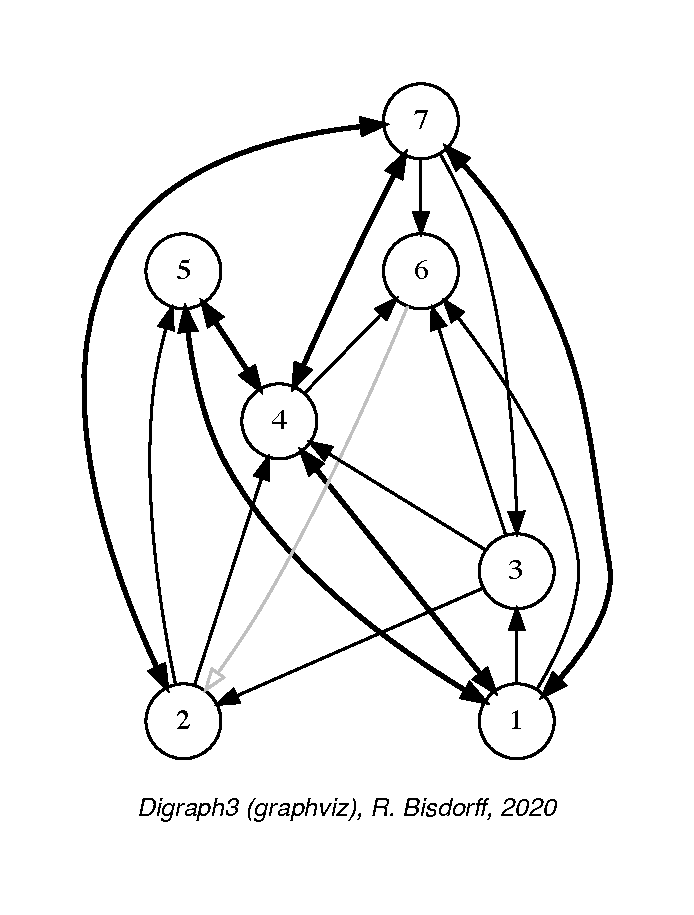
\includegraphics[width=6cm]{Figures/2-1-tutRandValDigraph.pdf}
\caption{\emph{The tutorial random valuation digraph}. Double links are drawn in bold black with an arrowhead at each end, whereas single asymmetric links are drawn in black with an arrowhead showing the direction of the link. Notice the undetermined relational situation ($r(6\,S\,2) = 0.00$) observed between nodes '6' and '2'. The corresponding link is marked in gray with an open arrowhead in the drawing}
\label{fig:2.1}       % Give a unique label
\end{figure}
  
\section{Asymmetric and symmetric parts}
\label{sec:2.3}

We may now extract both the \emph{}\emph{symmetric} as well as the \emph{asymmetric} part of digraph \texttt{rdg} with the help of two corresponding constructors (see List.~\vref{list:2.3}) \index{AsymmetricPartialDigraph@\texttt{AsymmetricPartialDigraph} class}\index{SymmetricPartialDigraph@\texttt{SymmetricPartialDigraph} class}.
\begin{lstlisting}[caption={Computing asymmetric and symmetric Parts},label=list:2.3]
>>> from digraphs import AsymmetricPartialDigraph,\
...                      SymmetricPartialDigraph
>>> asymDg = AsymmetricPartialDigraph(rdg)
>>> asymDg.exportGraphViz()
>>> symDg = SymmetricPartialDigraph(rdg)
>>> symDg.exportGraphViz()
\end{lstlisting}
\begin{figure}[ht]
  % \sidecaption
  Asymmetric Part \hfill Symmetric Part \\
  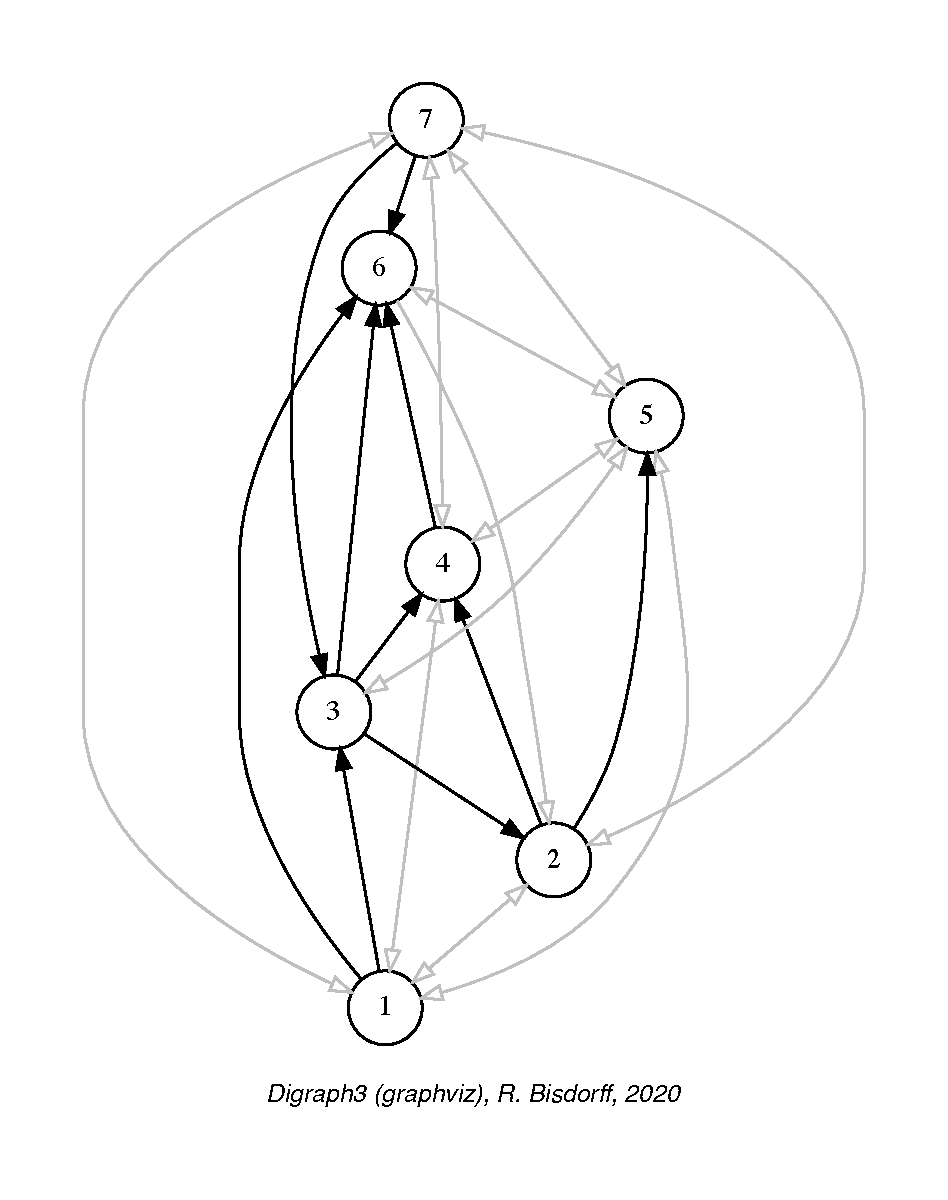
\includegraphics[height=6cm]{Figures/2-2-asymmetricPart.pdf}\hfill
  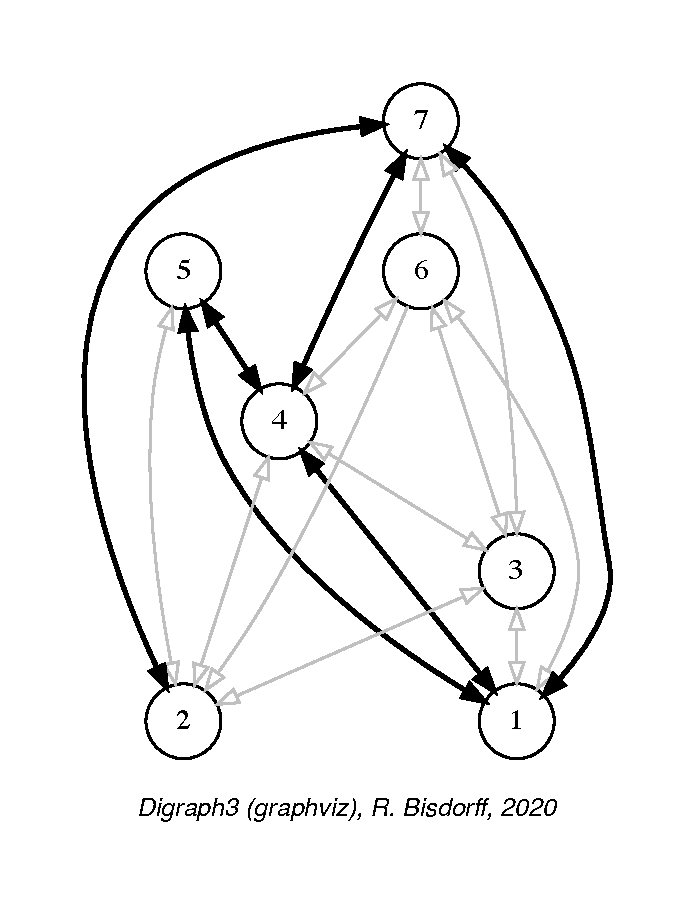
\includegraphics[height=6cm]{Figures/2-2-symmetricPart.pdf}\hfill
\caption{Asymmetric and symmetric part of the tutorial random valuation digraph}
\label{fig:2.2}       % Give a unique label
\end{figure}

The constructor of the partial objects \texttt{asymDg} and \texttt{symDg} puts to the indeterminate characteristic value all non-asymmetric, respectively non-symmetric links between nodes (see Fig.~\vref{fig:2.2}).

Here below, for illustration the source code of the \texttt{ relation} constructor of the \texttt{AsymmetricPartialDigraph} class.
\begin{lstlisting}[caption={Computing the asymmetric part of a bipolar-valued relation},label=list:2.4,basicstyle=\ttfamily\scriptsize]
def _constructRelation(self):
    actions = self.actions
    Min = self.valuationdomain['min']
    Max = self.valuationdomain['max']
    Med = self.valuationdomain['med']
    relationIn = self.relation
    relationOut = {}
    for a in actions:
	relationOut[a] = {}
	for b in actions:
	    if a != b:
                if relationIn[a][b] >= Med and relationIn[b][a] <= Med:
		    relationOut[a][b] = relationIn[a][b]
		elif relationIn[a][b] <= Med and relationIn[b][a] >= Med:
		    relationOut[a][b] = relationIn[a][b]
		else:
		    relationOut[a][b] = Med
	    else: # reflexive links are ignored
		relationOut[a][b] = Med
    return relationOut
\end{lstlisting}

\section{Border and inner parts}
\label{sec:2.4}

We may also extract the \emph{border} --the part of a digraph induced by the union of its initial and terminal prekernels (see Chap.~\ref{sec:17})--  as well as, the \emph{inner part} --the complement of the border-- with the help of two corresponding class constructors: \texttt{GraphBorder}\index{GraphBorder@\texttt{GraphBorder} class} and \texttt{GraphInner}\index{GraphInner@\texttt{GraphInner} class} (see Fig.~\vref{fig:2.3}).

\begin{figure}[ht]
%\sidecaption
  Border Part \hfill Inner Part \\
  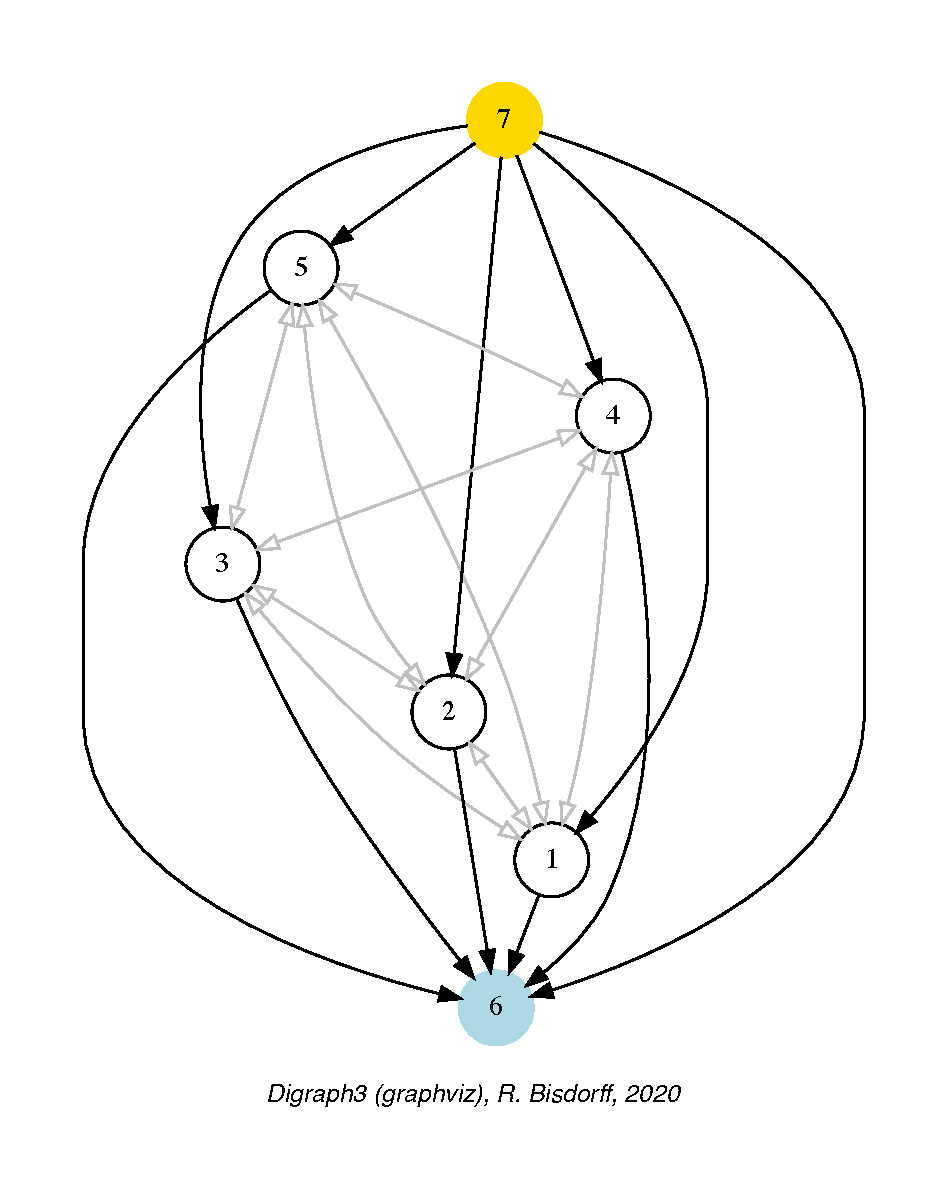
\includegraphics[height=6cm]{Figures/2-3-linearOrderBorder.pdf}\hfill
  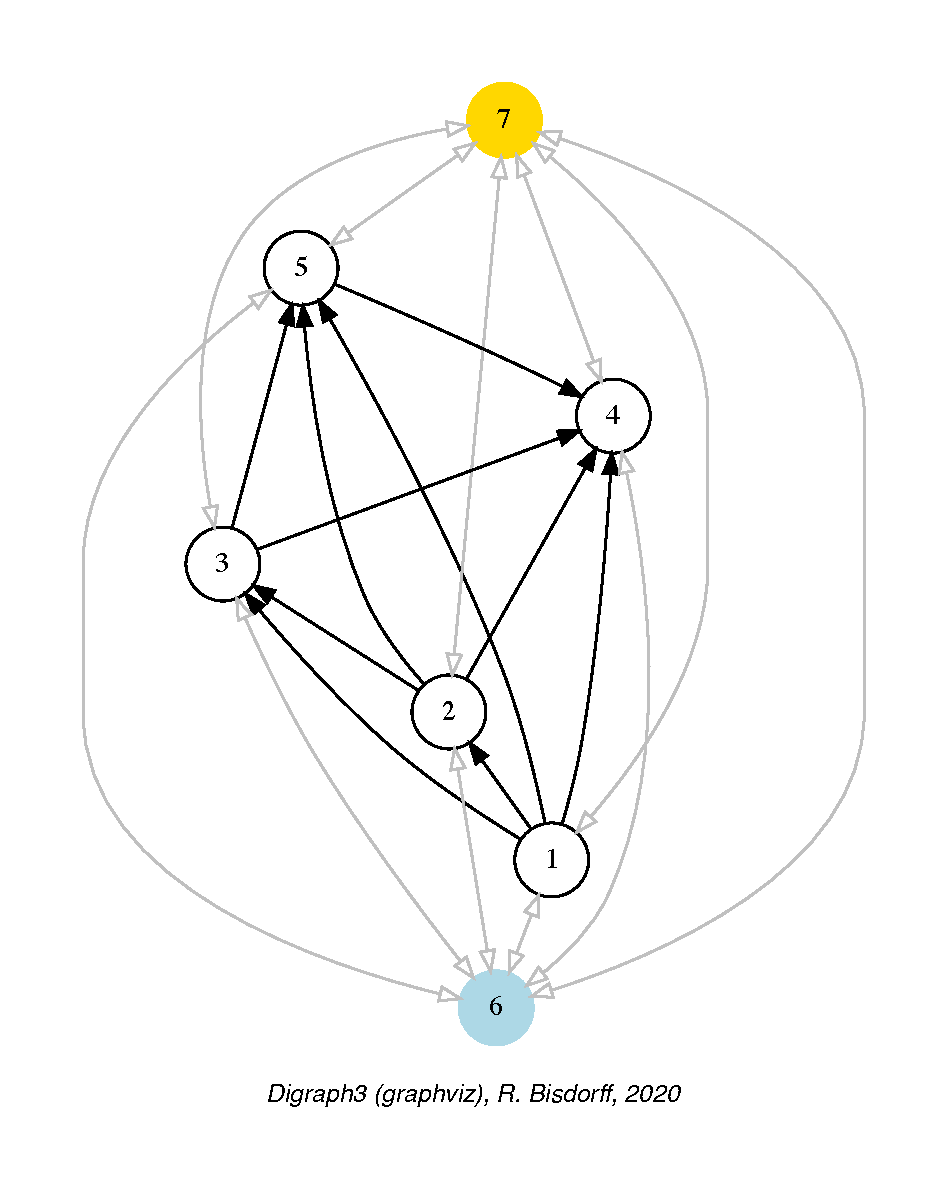
\includegraphics[height=6cm]{Figures/2-3-linearOrderInner.pdf}\hfill
\caption{\emph{Border} and \emph{inner} part of a linear order oriented by \emph{terminal} and \emph{initial} kernels.}
\label{fig:2.3}       % Give a unique label
\end{figure}
Let us illustrate the digraph border and inner parts on a linear ordering obtained from the tutorial random valuation digraph \texttt{rdg}  with the \NetFlows ranking rule  (see Sec.~\ref{sec:8.3}).  
\begin{lstlisting}[caption={Border and inner part of a linear order},label=list:2.5]
>>> from digraphs import GraphBorder, GraphInner
>>> from linearOrders import NetFlowsOrder
>>> nf = NetFlowsOrder(rdg)
>>> nf.netFlowsOrder
   ['6', '4', '5', '3', '2', '1', '7']
>>> bnf = GraphBorder(nf)
>>> bnf.exportGraphViz(lastChoice=['6'],firstChoice=['7'])
>>> inf = GraphInner(nf)
>>> inf.exportGraphViz(lastChoice=['6'],firstChoice=['7'])
\end{lstlisting}
We may orient the \texttt{graphviz} drawings in Figure~\vref{fig:2.3}  with the terminal node 6 (\texttt{lastChoice} parameter) and initial node 7 (\texttt{firstChoice} parameter) (see List.~\vref{list:2.5} Lines 7 and 9).

The constructor of the partial digraphs \texttt{bnf} and \texttt{inf}  (see Lines 3 and 6) puts to the \emph{indeterminate} characteristic value all links not in the \emph{border}, respectively \emph{not} in the \emph{inner} part (see Fig.~\vref{fig:2.3}). Being much {\em denser\/} than a linear order, the actual inner part of our tutorial random valuation digraph \texttt{rdg} is reduced to a single arc between nodes 3 and 4 (see Fig.~\vref{fig:2.4}). Indeed, a complete digraph on the limit has no inner part (privacy!) at all, whereas empty and indeterminate digraphs admit both, an empty border and an empty inner part.
\begin{figure}[h]
%\sidecaption
  Border Part \hfill Inner Part \\
  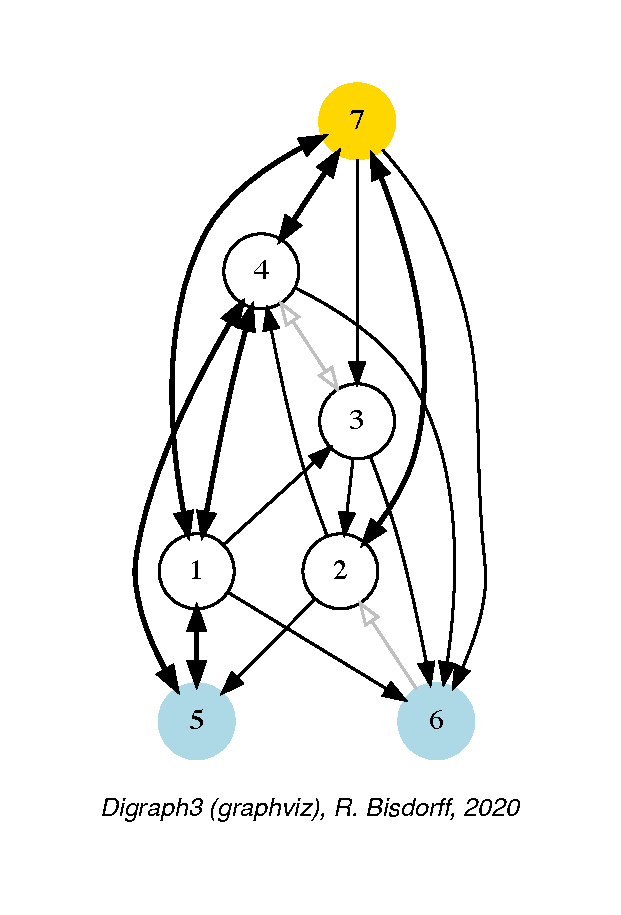
\includegraphics[height=6cm]{Figures/2-4-tutRandValDigraph_border.pdf}\hfill
  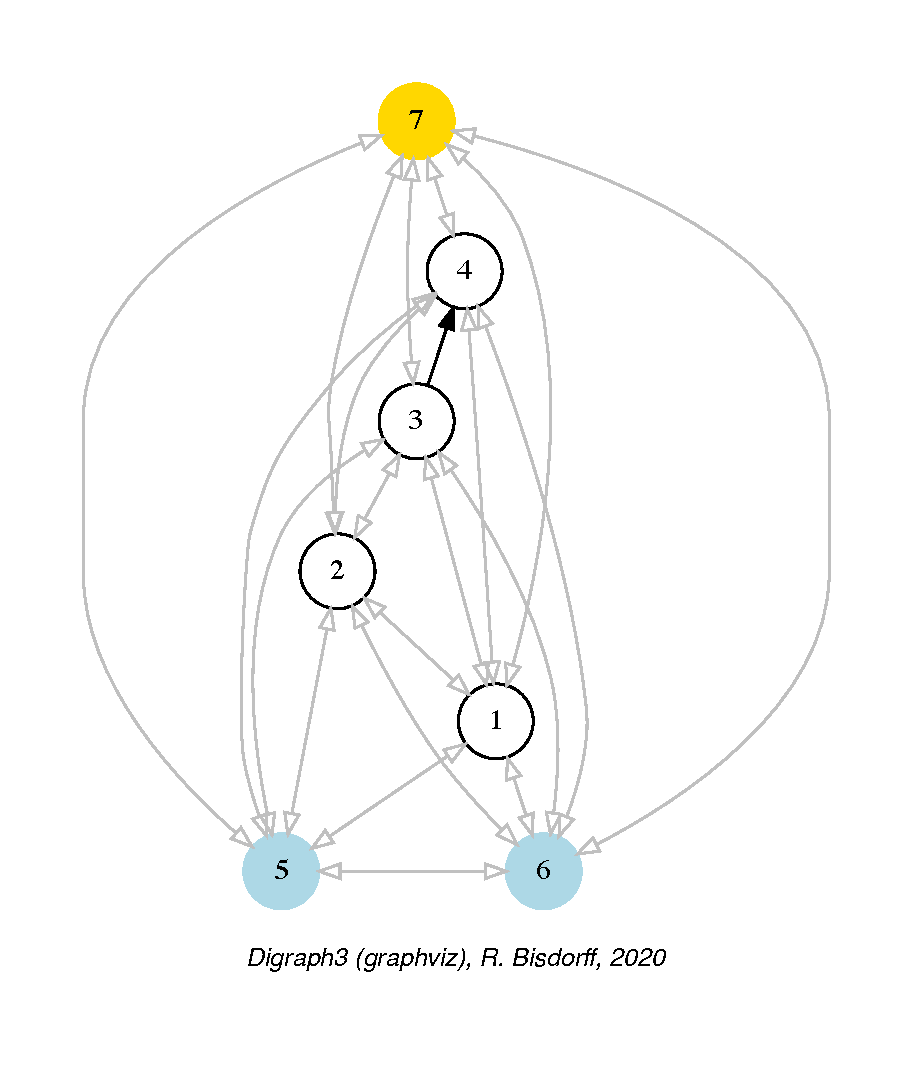
\includegraphics[height=6cm]{Figures/2-4-tutRandValDigraph_inner.pdf}\hfill
\caption{Border and inner part of the tutorial random valuation digraph \texttt{rdg}}
\label{fig:2.4}       % Give a unique label
\end{figure}

\section{Fusion by epistemic disjunction}
\label{sec:2.5}

We may recover object \texttt{rdg} from both partial objects \texttt{asymDg} and \texttt{symDg}, or as well from the border \texttt{bg} and the inner part \texttt{ig}, with a \emph{bipolar fusion} operator, also called \emph{epistemic disjunction}, available via the \texttt{FusionDigraph}\index{FusionDigraph@\texttt{FusionDigraph} class} class. 
\begin{lstlisting}[caption={Epistemic fusion of partial diagraphs},label=list:2.6]
>>> from digraphs import FusionDigraph
>>> fusDg = FusionDigraph(asymDg,symDg,operator='o-max')
>>> # fusDg = FusionDigraph(bg,ig,operator='o-max')
>>> fusDg.showRelationTable()
  * ---- Relation Table -----
   r(xSy) |  '1'    '2'   '3'  '4'   '5'    '6'  '7'	  
   -------|------------------------------------------
    '1'   |  0.00 -0.48  0.70  0.86  0.30  0.38  0.44	 
    '2'   | -0.22  0.00 -0.38  0.50  0.80 -0.54  0.02	 
    '3'   | -0.42  0.08  0.00  0.70 -0.56  0.84 -1.00	 
    '4'   |  0.44 -0.40 -0.62  0.00  0.04  0.66  0.76	 
    '5'   |  0.32 -0.48 -0.46  0.64  0.00 -0.22 -0.52	 
    '6'   | -0.84  0.00 -0.40 -0.96 -0.18  0.00 -0.22	 
    '7'   |  0.88  0.72  0.82  0.52 -0.84  0.04  0.00
\end{lstlisting}

The epistemic fusion operator \texttt{o-max} (see List.~\vref{list:2.6} Line 2) is defined as follows:
\begin{definition}[Disjunctive epistemic fusion operator \texttt{o-max}]\label{def:disjunctiveFusion}

\noindent Let $r$ and $r'$ characterise two bipolar-valued epistemic situations:
\begin{itemize}[leftmargin=0.5cm,rightmargin=0.5cm,nosep]
\item \texttt{o-max}$(r, r')$ = $\max(r, r' )$ when both $r$ and $r'$ are more or less valid or indeterminate;
\item \texttt{o-max}$(r, r')$ = $\min(r, r' )$ when both $r$ and $r'$ are more or less invalid or indeterminate;
\item \texttt{o-max}$(r, r')$ = $0.0$, i.e. indeterminate otherwise.
\end{itemize}
\end{definition}

Mind that the \texttt{o-max} operator, like a mean operator, is \emph{not associative} when more than 2 operands are given. In order to make the \texttt{o-max} fusion univocal, the following rule is applied: --first, all positive and negative terms are separately aggregated, --then the \texttt{o-max} fusion is applied on both aggregates.

\section{Dual, converse and codual digraphs}
\label{sec:2.6}

We may as readily compute the \emph{dual}\index{DualDigraph@\texttt{DualDigraph} class} (negated relation \footnote{Not to be confused with the dual graph of a plane graph $g$ that has a vertex for each face of $g$. Here we mean the \emph{less than} (strict converse) relation corresponding to a \emph{greater or equal} relation, or the \emph{less than or equal} relation corresponding to a (strict) \emph{better than} relation.}), the \emph{converse}\index{ConverseDigraph@\texttt{ConverseDigraph} class} (transposed relation) and the \emph{codual}\index{CoDualDigraph@\texttt{CoDualDigraph} class} (transposed and negated relation) of the digraph instance \texttt{rdg}. 
\begin{lstlisting}[caption={Computing associated dual, converse and codual digraphs},label=list:2.7]
>>> from digraphs import\
...          DualDigraph, ConverseDigraph, CoDualDigraph
>>> # dual of rdg
>>> ddg = DualDigraph(rdg)
>>> ddg.showRelationTable()
    -r(xSy) |  '1'    '2'   '3'  '4'   '5'    '6'  '7'	  
    --------|------------------------------------------
    '1 '    |  0.00  0.48 -0.70 -0.86 -0.30 -0.38 -0.44	 
    '2'     |  0.22  0.00  0.38 -0.50  0.80  0.54 -0.02	 
    '3'     |  0.42  0.08  0.00 -0.70  0.56 -0.84  1.00	 
    '4'     | -0.44  0.40  0.62  0.00 -0.04 -0.66 -0.76	 
    '5'     | -0.32  0.48  0.46 -0.64  0.00  0.22  0.52	 
    '6'     |  0.84  0.00  0.40  0.96  0.18  0.00  0.22	 
    '7'     |  0.88 -0.72 -0.82 -0.52  0.84 -0.04  0.00
>>> # converse of rdg
>>> cdg = ConverseDigraph(rdg)
>>> cdg.showRelationTable()
    * ---- Relation Table -----
     r(ySx) |  '1'    '2'   '3'   '4'   '5'   '6'   '7'	  
    --------|------------------------------------------
    '1'     |  0.00 -0.22 -0.42  0.44  0.32 -0.84  0.88	 
    '2'     | -0.48  0.00  0.08 -0.40 -0.48  0.00  0.72	 
    '3'     |  0.70 -0.38  0.00 -0.62 -0.46 -0.40  0.82	 
    '4'     |  0.86  0.50  0.70  0.00  0.64 -0.96  0.52	 
    '5'     |  0.30  0.80 -0.56  0.04  0.00 -0.18 -0.84	 
    '6'     |  0.38 -0.54  0.84  0.66 -0.22  0.00  0.04	 
    '7'     |  0.44  0.02 -1.00  0.76 -0.52 -0.22  0.00	 
>>> # codual of rdg
>>> cddg = CoDualDigraph(rdg)
>>> cddg.showRelationTable()
    * ---- Relation Table -----
    -r(ySx) |  '1'    '2'   '3'   '4'   '5'   '6'   '7'	    
    --------|------------------------------------------
    '1'     |  0.00  0.22  0.42 -0.44 -0.32  0.84 -0.88	 
    '2'     |  0.48  0.00 -0.08  0.40  0.48  0.00 -0.72	 
    '3'     | -0.70  0.38  0.00  0.62  0.46  0.40 -0.82	 
    '4'     | -0.86 -0.50 -0.70  0.00 -0.64  0.96 -0.52	 
    '5'     | -0.30 -0.80  0.56 -0.04  0.00  0.18  0.84	 
    '6'     | -0.38  0.54 -0.84 -0.66  0.22  0.00 -0.04	 
    '7'     | -0.44 -0.02  1.00 -0.76  0.52  0.22  0.00	 
\end{lstlisting}

Computing the \emph{dual}, respectively the \emph{converse} of a digraph, may also be done with prefixing the \texttt{\_\_neg\_\_} ($-$) or the \texttt{\_\_invert\_\_} ($\sim$) operator. The \emph{codual} of a \texttt{Digraph} object may, hence, as well be computed with a \emph{composition} (in either order) of both operations.
\begin{lstlisting}[caption={Computing the dual, the converse and the codual of a digraph},label=list:2.8]
>>> ddg = -rdg   # dual of rdg
>>> cdg = ~rdg   # converse of rdg
>>> cddg = ~(-rdg) # = -(~(rdg) codual of rdg
>>> (-(~rdg)).showRelationTable()
  * ---- Relation Table -----
   -r(ySx) |  '1'    '2'   '3'   '4'   '5'   '6'   '7'	    
   --------|------------------------------------------
   '1'     |  0.00  0.22  0.42 -0.44 -0.32  0.84 -0.88	 
   '2'     |  0.48  0.00 -0.08  0.40  0.48  0.00 -0.72	 
   '3'     | -0.70  0.38  0.00  0.62  0.46  0.40 -0.82	 
   '4'     | -0.86 -0.50 -0.70  0.00 -0.64  0.96 -0.52	 
   '5'     | -0.30 -0.80  0.56 -0.04  0.00  0.18  0.84	 
   '6'     | -0.38  0.54 -0.84 -0.66  0.22  0.00 -0.04	 
   '7'     | -0.44 -0.02  1.00 -0.76  0.52  0.22  0.00	 
\end{lstlisting}
  
\section{Symmetric and transitive closures}
\label{sec:2.7}

Symmetric and transitive closures, by default in-site methods, are also available (see Fig.~\vref{fig:2.5})\index{closeSymmetric@\texttt{closeSymmetric()}}\index{closeTransitive@\texttt{closeTransitive()}}. Note that it is a good idea, before going ahead with these in-site operations, who irreversibly modify the original \texttt{rdg} object, to previously make a backup version of \texttt{rdg}. The simplest storage method, always provided by the generic \texttt{Digraph.save()} method, writes out in a named file the python content of the Digraph object in string representation (see Sec.~\vref{sec:1.3}).
\begin{lstlisting}[caption={Symmeric and transitive closures},label=list:2.9]
>>> rdg.save('tutRandValDigraph')
>>> rdg.closeSymmetric(InSite=True)
>>> rdg.closeTransitive(InSite=True)
>>> rdg.exportGraphViz('strongComponents')
\end{lstlisting}
\begin{figure}[h]
\sidecaption[t]
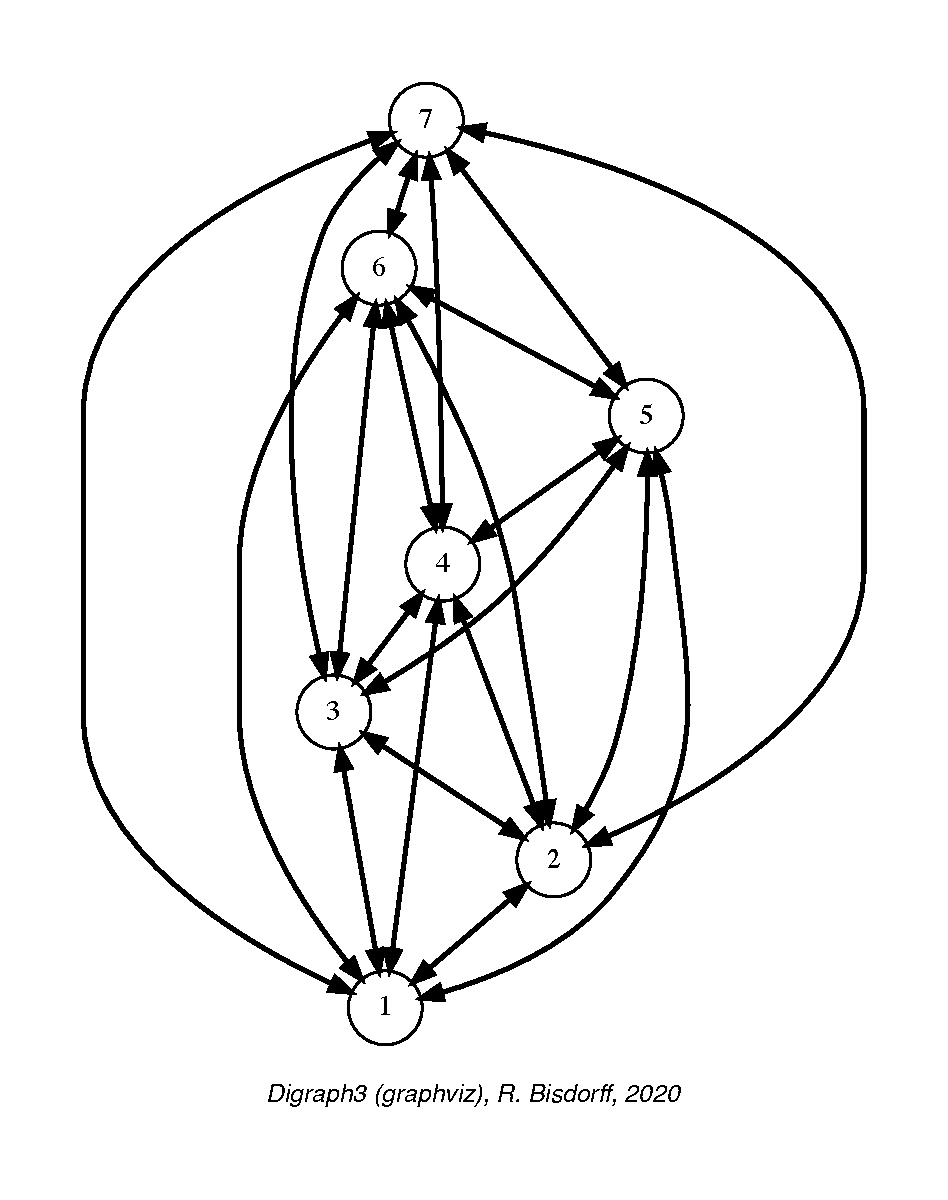
\includegraphics[width=6cm]{Figures/2-5-strongComponents.pdf}
\caption{Symmetric and transitive closure of the tutorial random valuation digraph $rdg$.}
\label{fig:2.5}       % Give a unique label
\end{figure}

The \texttt{closeSymmetric()}\index{closeSymmetric@\texttt{closeSymmetric()}} method (see List.~\vref{list:2.9} Line 2), of complexity $O(n^2)$ where $n$ denotes the digraph's order, changes, on the one hand, all single pairwise links it may detect into double links by operating a disjunction of the pairwise relations. On the other hand, the \texttt{closeTransitive()}\index{closeTransitive@\texttt{closeTransitive()}}  method (see Line 3), implements the \emph{Roy-Warshall} transitive closure algorithm of complexity $O(n^3)$ \index{Roy@\textsl{B. Roy}} \index{warshall@\textsl{S. Warshall}} (\citealp{ROY-1959} and \citealp{WAR-1962}).

The same \texttt{closeTransitive()} with a \texttt{Reverse = True} flag may be readily used for eliminating all transitive arcs from a transitive digraph instance. We make usage of this feature when drawing Hasse diagrams of \texttt{TransitiveDigraph}\index{TransitiveDigraph@\texttt{TransitiveDigraph} class} objects.

\section{Strong components}
\label{sec:2.8}

As the original digraph \texttt{rdg} was connected (see above the result of the showShort() command), both the symmetric and the transitive closures operated together, will necessarily produce a single strong component, i.e. a \textbf{complete} digraph. We may sometimes wish to collapse all strong components in a given digraph and construct the so \emph{collapsed} digraph. Using the \texttt{StrongComponentsCollapsedDigraph} constructor \index{StrongComponentsCollapsedDigraph@\texttt{StrongComponentsCollapsedDigraph} class} here will render a single hyper-node gathering all the original nodes (see Line 7 below).
\begin{lstlisting}[caption={Computing the strong components in a digraph},label=list:2.10]
>>> from digraphs import StrongComponentsCollapsedDigraph
>>> sc = StrongComponentsCollapsedDigraph(rdg)
>>> sc.showAll()
  *----- show detail -----*
   Digraph          : tutRandValDigraph_Scc
  *---- Actions ----*
    ['_7_1_2_6_5_3_4_']
  *---- Relation Table -----
      S     |  'Scc_1'	  
     -------|---------
     'Scc_1' |  0.00
  *---- strong Components ----*
   short 	 content
   'Scc_1' 	 '_7_1_2_6_5_3_4_'
  *---- Neighborhoods ----*
   Gamma     :
   'frozenset({'7','1','2','6','5','3','4'})':
                     in => set(), out => set()
   Not Gamma :
   'frozenset({'7','1','2','6','5','3','4'})':
                     in => set(), out => set()
\end{lstlisting}
  
\section{CSV storage}
\label{sec:2.9}

Sometimes it is required to exchange the graph valuation data in CSV format with a statistical package like \textbf{R}\footnote{\url{https://www.r-project.org/}}. For this purpose it is possible to export the digraph data into a CSV file. The valuation domain is hereby normalised by default to the range $[-1.0,1.0]$ and the diagonal is put by default to the minimal value $-1.0$.
\begin{lstlisting}
>>> rdg = Digraph('tutRandValDigraph')
>>> rdg.saveCSV('tutRandValDigraph')
  # content of file tutRandValDigraph.csv
  "d","1","2","3","4","5","6","7"
  "1",-1.0,0.48,-0.7,-0.86,-0.3,-0.38,-0.44
  "2",0.22,-1.0,0.38,-0.5,-0.8,0.54,-0.02
  "3",0.42,-0.08,-1.0,-0.7,0.56,-0.84,1.0
  "4",-0.44,0.4,0.62,-1.0,-0.04,-0.66,-0.76
  "5",-0.32,0.48,0.46,-0.64,-1.0,0.22,0.52
  "6",0.84,0.0,0.4,0.96,0.18,-1.0,0.22
  "7",-0.88,-0.72,-0.82,-0.52,0.84,-0.04,-1.0
\end{lstlisting}
  
It is possible to reload a \texttt{Digraph} instance from its previously saved CSV file content.
\begin{lstlisting} 
>>> from digraphs import CSVDigraph   
>>> rdgcsv = CSVDigraph('tutRandValDigraph')
>>> rdgcsv.showRelationTable(ReflexiveTerms=False)
    * ---- Relation Table -----
    r(xSy) |   '1'   '2'   '3'   '4'   '5'   '6'   '7'	  
    -------|------------------------------------------------------------
    '1'    |   -   -0.48  0.70  0.86  0.30  0.38  0.44	 
    '2'    | -0.22   -   -0.38  0.50  0.80 -0.54  0.02	 
    '3'    | -0.42  0.08   -    0.70 -0.56  0.84 -1.00	 
    '4'    |  0.44 -0.40 -0.62   -    0.04  0.66  0.76	 
    '5'    |  0.32 -0.48 -0.46  0.64   -   -0.22 -0.52	 
    '6'    | -0.84  0.00 -0.40 -0.96 -0.18   -   -0.22	 
    '7'    |  0.88  0.72  0.82  0.52 -0.84  0.04   -
\end{lstlisting}
  
It is as well possible to show a coloured version of the valued relation table in a system browser window tab (see Fig.~\vref{fig:2.5}).
\begin{lstlisting}
>>> rdgcsv.showHTMLRelationTable(tableTitle="Tutorial random digraph")
\end{lstlisting}
 \begin{figure}[ht]
\sidecaption[t]
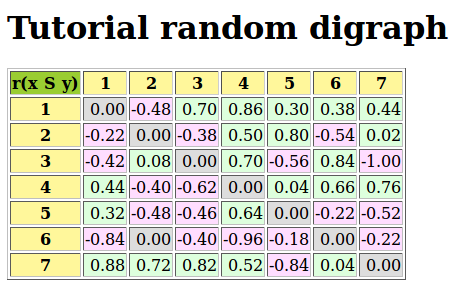
\includegraphics[width=7cm]{Figures/2-6-htmlTutorialDigraph.png}
\caption{The valued relation table shown in a browser window. Positive arcs are shown in green and negative arcs in red. Indeterminate --zero-valued-- links, like the reflexive diagonal ones or the link between node \texttt{'6'} and node \texttt{'2'}, are shown in gray}
\label{fig:2.6}       % Give a unique label
\end{figure}
 
\section{Complete, empty and indeterminate digraphs}
\label{sec:2.10}

Let us finally mention some special universal classes of digraphs that are readily available in the \texttt{digraphs} module\footnote{See \citealp{BIS-2021}}, like:
\begin{itemize}[nosep]
\item the \texttt{CompleteDigraph}\index{CompleteDigraph@\texttt{CompleteDigraph} class},
\item  the \texttt{EmptyDigraph}\index{EmptyDigraph@\texttt{EmptyDigraph} class} and
\item  the \texttt{IndeterminateDigraph}\index{IndeterminateDigraph@\texttt{IndeterminateDigraph} class} class,
\end{itemize}
who put all characteristic values respectively to the \emph{maximum}, the \emph{minimum} or the \emph{median} indeterminate characteristic value.
\begin{lstlisting}[caption={Complete, empty and indeterminate digraphs},label=list:2.11]
>>> from digraphs import CompleteDigraph,EmptyDigraph,\
...   			 IndeterminateDigraph
>>> # the empty digraph   
>>> e = EmptyDigraph(order=5)
>>> e.showRelationTable()
    * ---- Relation Table -----
      S   |    '1'    '2'    '3'    '4'	   '5'	  
    ---- -|-----------------------------------
    '1'   |  -1.00  -1.00  -1.00  -1.00	 -1.00	 
    '2'   |  -1.00  -1.00  -1.00  -1.00	 -1.00	 
    '3'   |  -1.00  -1.00  -1.00  -1.00	 -1.00	 
    '4'   |  -1.00  -1.00  -1.00  -1.00	 -1.00	 
    '5'   |  -1.00  -1.00  -1.00  -1.00	 -1.00
>>> e.showNeighborhoods() 
    Neighborhoods:
      Gamma     :
    '1': in => set(), out => set()
    '2': in => set(), out => set()
    '5': in => set(), out => set()
    '3': in => set(), out => set()
    '4': in => set(), out => set()
      Not Gamma :
    '1': in => {'2','4','5','3'}, out => {'2','4','5','3'}
    '2': in => {'1','4','5','3'}, out => {'1','4','5','3'}
    '5': in => {'1','2','4','3'}, out => {'1','2','4','3'}
    '3': in => {'1','2','4','5'}, out => {'1','2','4','5'}
    '4': in => {'1','2','5','3'}, out => {'1','2','5','3'}
>>> # the indeterminate digraph
>>> i = IndeterminateDigraph()
    * ---- Relation Table -----
      S   |   '1'   '2'	  '3'	'4'   '5'	  
    ------|------------------------------
    '1'   |  0.00  0.00	 0.00  0.00  0.00	 
    '2'   |  0.00  0.00	 0.00  0.00  0.00	 
    '3'   |  0.00  0.00	 0.00  0.00  0.00	 
    '4'   |  0.00  0.00	 0.00  0.00  0.00	 
    '5'   |  0.00  0.00	 0.00  0.00  0.00	 
>>> i.showNeighborhoods()
    Neighborhoods:
      Gamma     :
    '1': in => set(), out => set()
    '2': in => set(), out => set()
    '5': in => set(), out => set()
    '3': in => set(), out => set()
    '4': in => set(), out => set()
      Not Gamma :
    '1': in => set(), out => set()
    '2': in => set(), out => set()
    '5': in => set(), out => set()
    '3': in => set(), out => set()
    '4': in => set(), out => set()
\end{lstlisting}

Mind the subtle difference between the neighbourhoods of an \emph{empty} and the neighbourhoods of an \emph{indeterminate} digraph instance. In the first kind, the neighbourhoods are known to be completely \emph{empty}  (see List.~\vref{list:2.11} Lines 22-27) whereas, in the latter, \emph{nothing is known} about the actual neighbourhoods of the nodes  (see Lines 46-51). These two cases illustrate why in the case of \emph{bipolar-valued} digraphs, we may sometimes need both a \texttt{gamma} \textbf{and} a \texttt{notGamma} attribute.

\vspace{1cm}
In the following Chapter~\ref{sec:3}  we introduce the main formal object of this book, namely \emph{bipolar-valued outranking} digraphs.

%%%%%%%%%%%%%%%%%%%%%%%%%%%%%%%%%%%%
\phantomsection
\addcontentsline{toc}{section}{Notes}
\section*{Notes}

It is \emph{D. Bouyssou} \index{Bouyssou@\emph{D. Bouyssou}} who first suggested us end of the nineties, when we started to work in Prolog on the computation of digraph kernels with finite domain constraint solvers, that the $50\%$ criteria significance majority was a special value to be carefully taken into account. The converging solution vectors of the fixpoint kernel equations confirmed this special status of the $50\%$ majority (see Chap.~\ref{sec:17}). These early insights led to the seminal articles on bipolar-valued epistemic logic where we introduced split truth/falseness semantics for a multi-valued logical processing of fuzzy preference modelling \citep{BIS-2000,BIS-2002}. The characteristic valuation domain remained however the classical fuzzy $[0.0;1.0]$ valuation domain.

It is only in 2004, when we succeeded in assessing the stability of the outranking digraph when solely ordinal criteria significance weights are given, that it became clear and evident for us that the characteristic valuation domain had to be shifted to a bipolar $[-1.0;+1.0]$-valued domain \citep{BIS-2004a}. In this bipolar valuation domain, the $50\%$ majority thershold corresponds now to the median $0.0$ value, characterising with the correct zero value an epistemic indetermination --no knowledge-- situation. Furthermore, identifying truth and falseness by the sign of the characteristic values revealed itself to be very efficient not only from a computational point of view, but also from scientific and semiotical perspectives. A positive (resp. negative) characteristic value now attest a logically valid (resp. invalid) statement and a negative affirmation now corresponds to a positive refutation. Furthermore, the median zero value gives way to efficiently handling partial digraphs --like the border or the assymetric part of a digraph-- and, even more important from a practical decision making point of view, any missing data.

The bipolar $[-1.0;+1.0]$-valued characteritisc domain opened so the way to important new operations and concepts, like the disjunctive epistemic fusion operation seen in Section~\vref{sec:2.5} that confers the outranking digraph a logically and epistemically sound definition \citep{BIS-2013}. \Kendall 's ordinal correlation index could be extended to a bipolar-valued relational equivalence index between digraphs \citep{BIS-2012a}. Making usage of the bipolar-valued Gaussian error function naturally led to defining a bipolar-valued likelihood function, where a positive (resp. negative) value gives the likelihood of an affirmation (resp. a refutation) \citep{BIS-2014}.      

%%%%%%% The chapter bibliography
%\normallatexbib
%\clearpage
%\phantomsection
%\addcontentsline{toc}{section}{Chapter Bibliograhy}
\bibliographystyle{spbasic}
%\typeout{}
\bibliography{03-backMatters/reference}
%\chapter{Working with bipolar-valued digraphs}
\label{sec:2}

\abstract*{ The chapter introduces bipolar-valued digraphs, the fondamental root type of all the specialised digraphs implemented in the \Digraph modules. With the help of a randomly valued digraph, we illustrate some basic digraph manipulation methods, like drawing the digraph, dividing the digraph into its asymmetric and symmetric parts, separating the border from the inner part, computing associated dual, converse and codual digraphs, and operating symmetric and transitive closures.}

\abstract{ The chapter introduces bipolar-valued digraphs, the fondamental root type of all the specialised digraphs implemented in the \Digraph modules. With the help of a randomly valued digraph, we illustrate some basic digraph manipulation methods, like drawing the digraph, dividing the digraph into its asymmetric and symmetric parts, separating the border from the inner part, computing associated dual, converse and codual digraphs, and operating symmetric and transitive closures.}

\section{Random bipolar-valued digraphs}

In Listing~\vref{list:2.1}, we generate a uniformly random $[-1.0; +1.0]$-valued digraph of order 7, denoted \texttt{rdg} and modelling, for instance, a binary relation $S(x,y)$ defined on the set of nodes of \texttt{rdg}. For this purpose, the \Digraph resources provide in the \texttt{randomDigraphs}\index{randomDigraphs@\texttt{randomDigraphs} module} module a specific \texttt{RandomValuationDigraph}\index{RandomValuationDigraph@\texttt{RandomValuationDigraph} class} class \citep{BIS-2021b}.
\begin{lstlisting}[caption={Random bipolar-valued digraph instance},label=list:2.1]
>>> from randomDigraphs import RandomValuationDigraph
>>> rdg = RandomValuationDigraph(order=7)
>>> rdg.save('tutRandValDigraph')
>>> from digraphs import Digraph
>>> rdg = Digraph('tutRandValDigraph')
>>> rdg
  *------- Digraph instance description ------*
   Instance class      : Digraph
   Instance name       : tutRandValDigraph
   Digraph Order       : 7
   Digraph Size        : 22
   Valuation domain    : [-1.00;1.00]
   Determinateness (%) : 75.24
   Attributes          : ['name','actions','order',
                          'valuationdomain','relation',
                          'gamma','notGamma']
\end{lstlisting}   

With the \texttt{save()} \index{save@\texttt{save()}} method (see Line 3) we keep for future use a backup version of \texttt{rdg} which is saved into a file named \texttt{tutRandValDigraph.py} in the current working directory. The genuine \texttt{Digraph} class constructor may restore the \texttt{rdg} object from the stored file (Lines 4-5). We may easily inspect the content of \texttt{rdg} (Line 6). The digraph size 22 indicates the number of positively valued arcs. The valuation domain is uniformly distributed in the interval $[-1.0; 1.0]$ and the mean absolute arc valuation is $(0.7524 \times 2)\, -\, 1.0 \;=\; 0.5048$ (Line 13).

As mentioned in the previous Chapter~\ref{sec:1}, all objects of \texttt{Digraph} type contain at least the list of attributes shown here in Lines 14-16: --a \texttt{name} (string), --a dictionary of \texttt{actions} (digraph nodes), --an \texttt{order} (integer) attribute containing the number of actions, --a \texttt{valuationdomain} dictionary, --a double dictionary \texttt{relation} representing the adjacency table of the digraph relation, --a \texttt{gamma} and --a {\tt notGamma} dictionary containing the direct neighbourhood of each action.

The \texttt{Digraph} class provides some generic \texttt{show...()} methods for exploring the content of a given \texttt{ Digraph} object, like the \texttt{showRelationTable()}\index{showRelationTable@\texttt{showRelationTable()}}, the \texttt{showComponents()}\index{showComponents@\texttt{showComponents()}} and the \texttt{showNeighborhoods()}\index{showNeighborhoods@\texttt{showNeighborhoods()}} methods.
\begin{lstlisting}[caption={Example of random valuation digraph},label=list:2.2]
>>> rdg.showRelationTable()
  * ---- Relation Table -----
   r(xSy) |  '1'    '2'   '3'  '4'   '5'    '6'  '7'	  
   -------|-------------------------------------------
    '1'   |  0.00 -0.48  0.70  0.86  0.30  0.38  0.44	 
    '2'   | -0.22  0.00 -0.38  0.50  0.80 -0.54  0.02	 
    '3'   | -0.42  0.08  0.00  0.70 -0.56  0.84 -1.00	 
    '4'   |  0.44 -0.40 -0.62  0.00  0.04  0.66  0.76	 
    '5'   |  0.32 -0.48 -0.46  0.64  0.00 -0.22 -0.52	 
    '6'   | -0.84  0.00 -0.40 -0.96 -0.18  0.00 -0.22	 
    '7'   |  0.88  0.72  0.82  0.52 -0.84  0.04  0.00
>>> rdg.showComponents()
  *--- Connected Components ---*
  1: ['1', '2', '3', '4', '5', '6', '7']
>>> rdg.showNeighborhoods()
  *---- Neighborhoods ------*
     Gamma:
     '1': in => {'5','7','4'}, out => {'5','7','6','3','4'}
     '2': in => {'7','3'},out => {'5','7','4'}
     '3': in => {'7','1'}, out => {'6','2','4'}
     '4': in => {'5','7','1','2','3'}, out => {'5','7','1','6'}
     '5': in => {'1','2','4'}, out => {'1','4'}
     '6': in => {'7','1','3','4'}, out => set()
     '7': in => {'1','2','4'}, out => {'1','2','3','4','6'}
     Not Gamma:
     '1': in => {'6','2','3'}, out => {'2'}
     '2': in => {'5','1','4'}, out => {'1','6','3'}
     '3': in => {'5','6','2','4'}, out => {'5','7','1'}
     '4': in => {'6'}, out => {'2','3'}
     '5': in => {'7','6','3'}, out => {'7','6','2','3'}
     '6': in => {'5','2'}, out => {'5','7','1','3','4'}
     '7': in => {'5','6','3'}, out => {'5'}
\end{lstlisting}   

Mind that some \texttt{Digraph} class methods will ignore the \emph{reflexive} links by considering that they are \emph{indeterminate}, i.e. the characteristic value $r(x\,S\,x)$ for all action $x$ is set to the \emph{median}, i.e. \emph{indeterminate} value $0.0$ in this case (see Listing~\vref{list:2.2} Lines 5-11 and \citet{BIS-2004a}).

\section{Graphviz drawings}
\label{sec:2.2}

An even better insight into the \texttt{Digraph} object \texttt{rdg} is given by looking at its \href{https://graphviz.org/}{graphviz} drawing \citep{graphviz}\footnote{The \texttt{exportGraphViz()} method is depending on drawing tools from the graphviz software (https://graphviz.org/). On Linux Ubuntu or Debian you may try \texttt{sudo apt-get install graphviz} to install them. There are ready \emph{dmg} installers for Mac OSX.}\index{graphviz}.
\begin{lstlisting}
>>> rdg.exportGraphViz('tutRandValDigraph')
 *---- exporting a dot file for GraphViz tools ------*
  Exporting to tutRandValDigraph.dot
  dot -Grankdir=BT -Tpng tutRandValDigraph.dot\
                           -o tutRandValDigraph.png
\end{lstlisting}
\begin{figure}[ht]
\sidecaption[t]
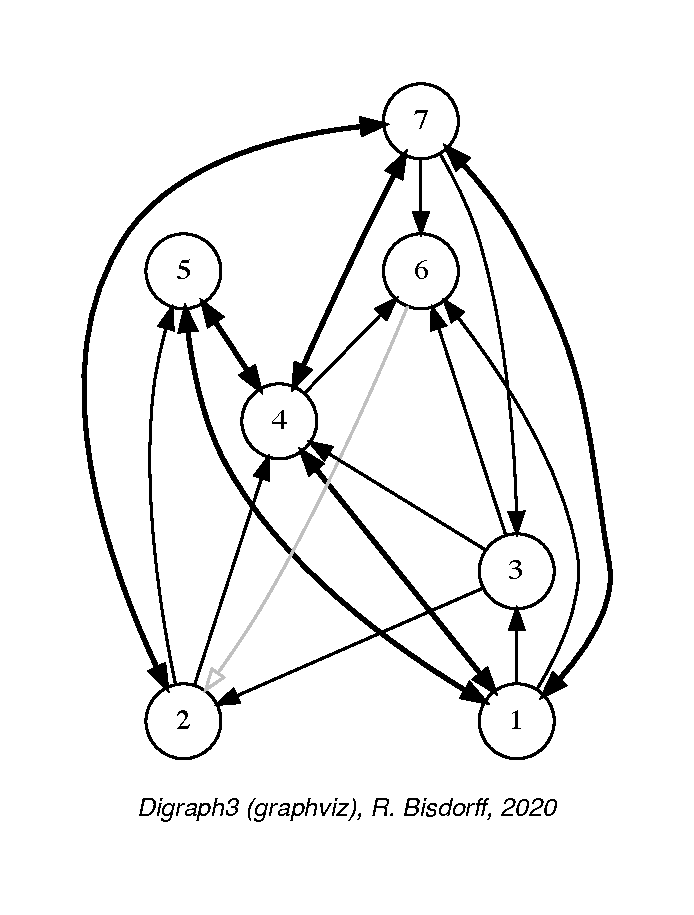
\includegraphics[width=6cm]{Figures/2-1-tutRandValDigraph.pdf}
\caption{\emph{The tutorial random valuation digraph}. Double links are drawn in bold black with an arrowhead at each end, whereas single asymmetric links are drawn in black with an arrowhead showing the direction of the link. Notice the undetermined relational situation ($r(6\,S\,2) = 0.00$) observed between nodes '6' and '2'. The corresponding link is marked in gray with an open arrowhead in the drawing}
\label{fig:2.1}       % Give a unique label
\end{figure}
  
\section{Asymmetric and symmetric parts}
\label{sec:2.3}

We may now extract both the \emph{}\emph{symmetric} as well as the \emph{asymmetric} part of digraph \texttt{rdg} with the help of two corresponding constructors (see List.~\vref{list:2.3}) \index{AsymmetricPartialDigraph@\texttt{AsymmetricPartialDigraph} class}\index{SymmetricPartialDigraph@\texttt{SymmetricPartialDigraph} class}.
\begin{lstlisting}[caption={Computing asymmetric and symmetric Parts},label=list:2.3]
>>> from digraphs import AsymmetricPartialDigraph,\
...                      SymmetricPartialDigraph
>>> asymDg = AsymmetricPartialDigraph(rdg)
>>> asymDg.exportGraphViz()
>>> symDg = SymmetricPartialDigraph(rdg)
>>> symDg.exportGraphViz()
\end{lstlisting}
\begin{figure}[ht]
  % \sidecaption
  Asymmetric Part \hfill Symmetric Part \\
  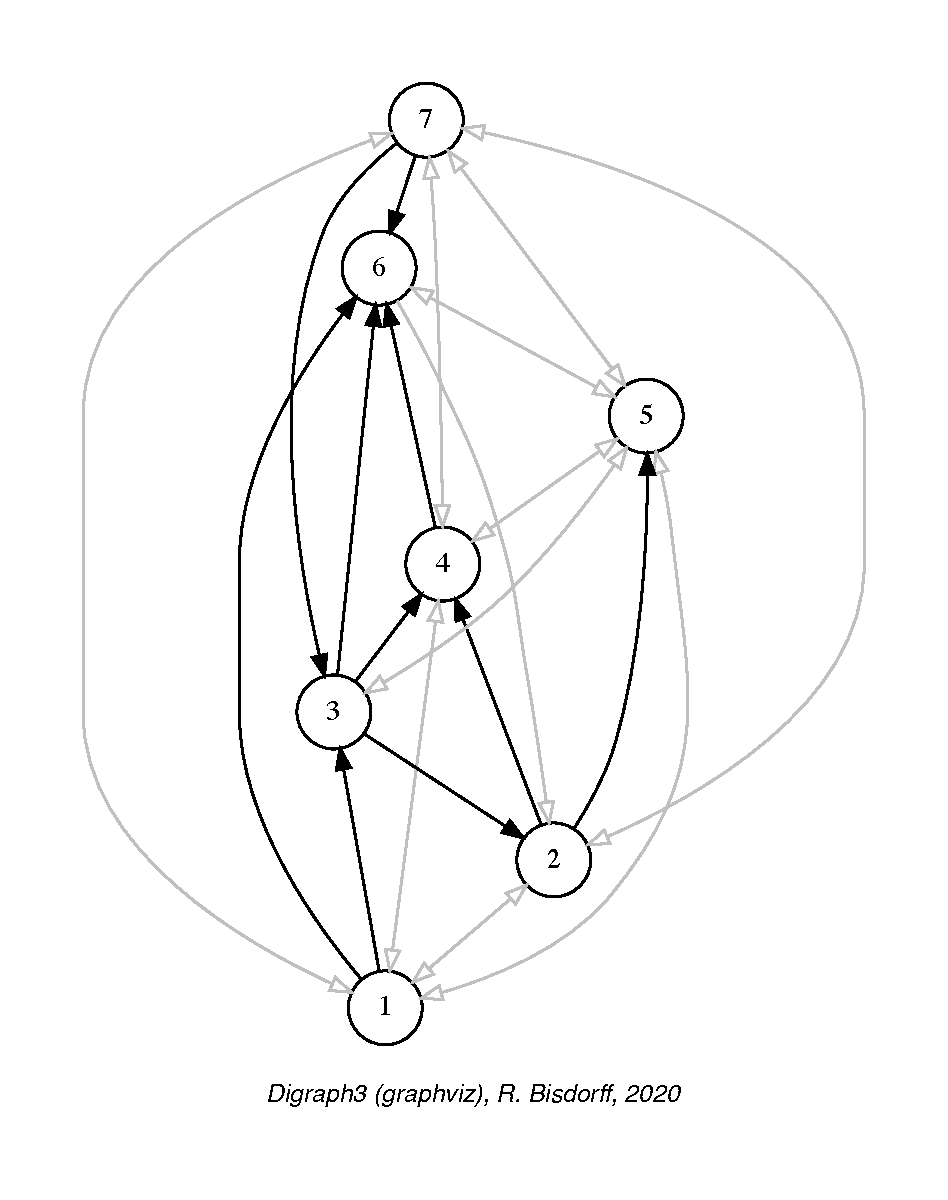
\includegraphics[height=6cm]{Figures/2-2-asymmetricPart.pdf}\hfill
  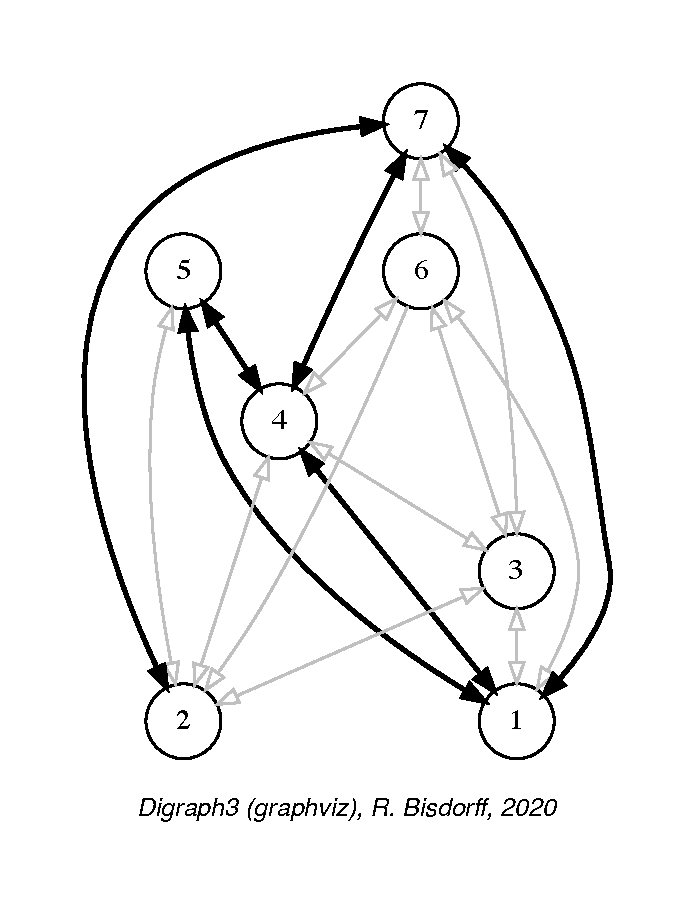
\includegraphics[height=6cm]{Figures/2-2-symmetricPart.pdf}\hfill
\caption{Asymmetric and symmetric part of the tutorial random valuation digraph}
\label{fig:2.2}       % Give a unique label
\end{figure}

The constructor of the partial objects \texttt{asymDg} and \texttt{symDg} puts to the indeterminate characteristic value all non-asymmetric, respectively non-symmetric links between nodes (see Fig.~\vref{fig:2.2}).

Here below, for illustration the source code of the \texttt{ relation} constructor of the \texttt{AsymmetricPartialDigraph} class.
\begin{lstlisting}[caption={Computing the asymmetric part of a bipolar-valued relation},label=list:2.4,basicstyle=\ttfamily\scriptsize]
def _constructRelation(self):
    actions = self.actions
    Min = self.valuationdomain['min']
    Max = self.valuationdomain['max']
    Med = self.valuationdomain['med']
    relationIn = self.relation
    relationOut = {}
    for a in actions:
	relationOut[a] = {}
	for b in actions:
	    if a != b:
                if relationIn[a][b] >= Med and relationIn[b][a] <= Med:
		    relationOut[a][b] = relationIn[a][b]
		elif relationIn[a][b] <= Med and relationIn[b][a] >= Med:
		    relationOut[a][b] = relationIn[a][b]
		else:
		    relationOut[a][b] = Med
	    else: # reflexive links are ignored
		relationOut[a][b] = Med
    return relationOut
\end{lstlisting}

\section{Border and inner parts}
\label{sec:2.4}

We may also extract the \emph{border} --the part of a digraph induced by the union of its initial and terminal prekernels (see Chap.~\ref{sec:17})--  as well as, the \emph{inner part} --the complement of the border-- with the help of two corresponding class constructors: \texttt{GraphBorder}\index{GraphBorder@\texttt{GraphBorder} class} and \texttt{GraphInner}\index{GraphInner@\texttt{GraphInner} class} (see Fig.~\vref{fig:2.3}).

\begin{figure}[ht]
%\sidecaption
  Border Part \hfill Inner Part \\
  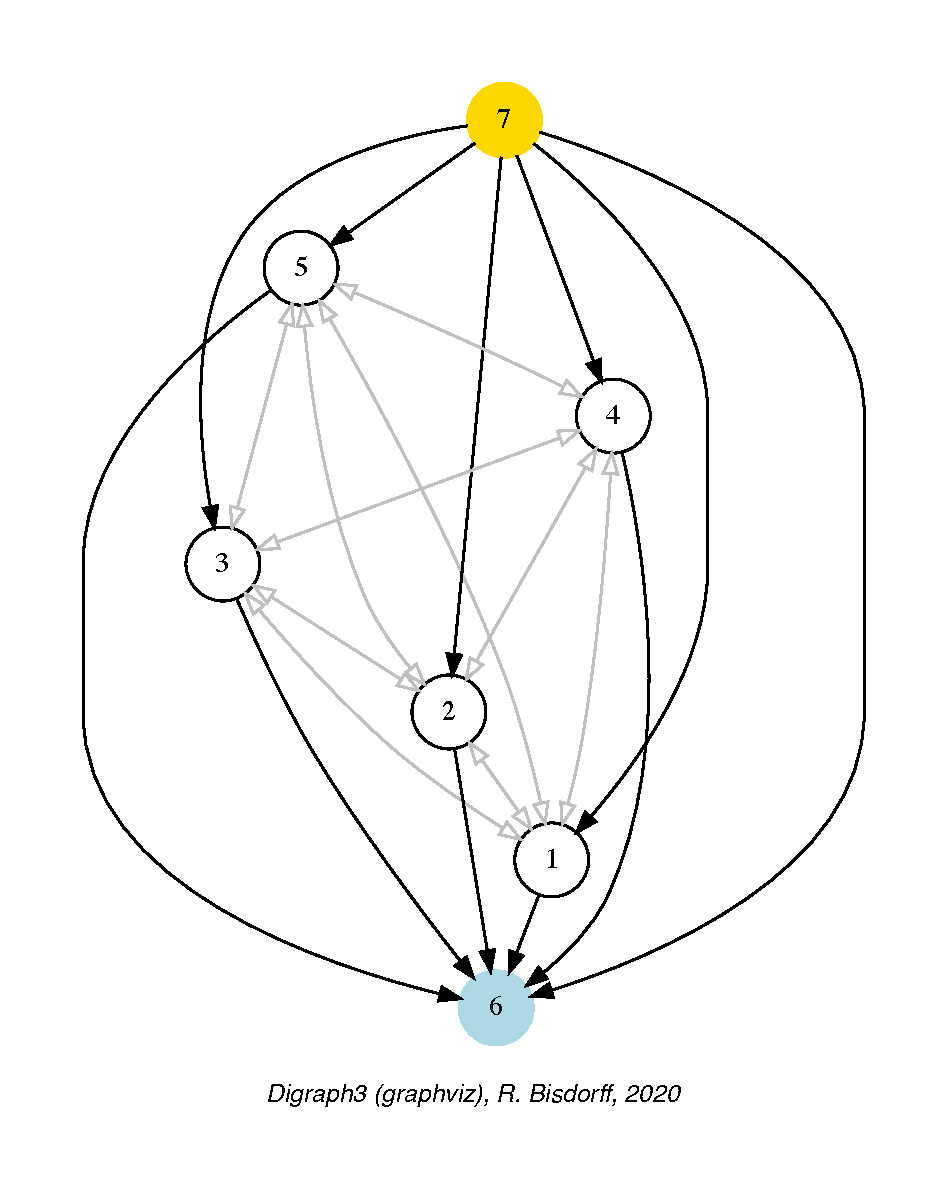
\includegraphics[height=6cm]{Figures/2-3-linearOrderBorder.pdf}\hfill
  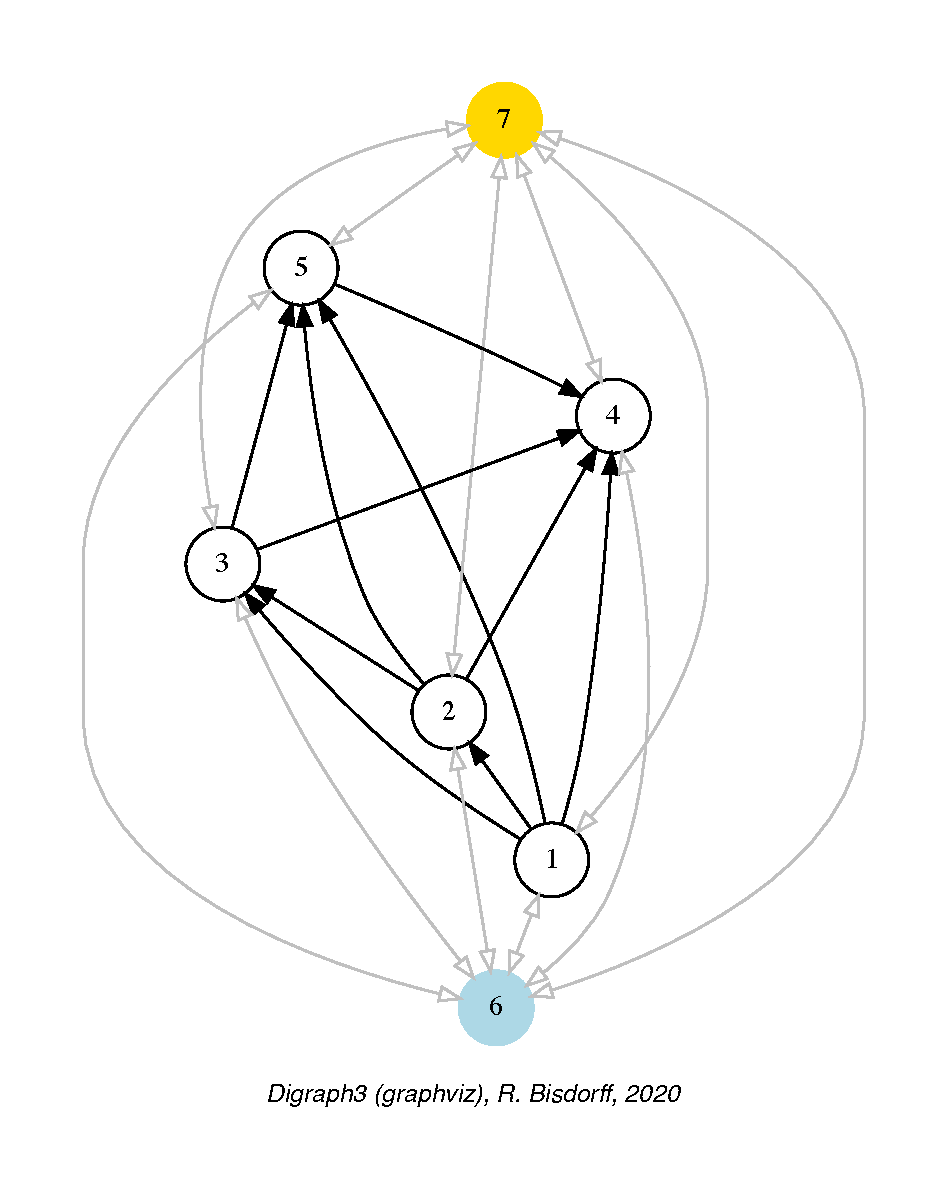
\includegraphics[height=6cm]{Figures/2-3-linearOrderInner.pdf}\hfill
\caption{\emph{Border} and \emph{inner} part of a linear order oriented by \emph{terminal} and \emph{initial} kernels.}
\label{fig:2.3}       % Give a unique label
\end{figure}
Let us illustrate the digraph border and inner parts on a linear ordering obtained from the tutorial random valuation digraph \texttt{rdg}  with the \NetFlows ranking rule  (see Sec.~\ref{sec:8.3}).  
\begin{lstlisting}[caption={Border and inner part of a linear order},label=list:2.5]
>>> from digraphs import GraphBorder, GraphInner
>>> from linearOrders import NetFlowsOrder
>>> nf = NetFlowsOrder(rdg)
>>> nf.netFlowsOrder
   ['6', '4', '5', '3', '2', '1', '7']
>>> bnf = GraphBorder(nf)
>>> bnf.exportGraphViz(lastChoice=['6'],firstChoice=['7'])
>>> inf = GraphInner(nf)
>>> inf.exportGraphViz(lastChoice=['6'],firstChoice=['7'])
\end{lstlisting}
We may orient the \texttt{graphviz} drawings in Figure~\vref{fig:2.3}  with the terminal node 6 (\texttt{lastChoice} parameter) and initial node 7 (\texttt{firstChoice} parameter) (see List.~\vref{list:2.5} Lines 7 and 9).

The constructor of the partial digraphs \texttt{bnf} and \texttt{inf}  (see Lines 3 and 6) puts to the \emph{indeterminate} characteristic value all links not in the \emph{border}, respectively \emph{not} in the \emph{inner} part (see Fig.~\vref{fig:2.3}). Being much {\em denser\/} than a linear order, the actual inner part of our tutorial random valuation digraph \texttt{rdg} is reduced to a single arc between nodes 3 and 4 (see Fig.~\vref{fig:2.4}). Indeed, a complete digraph on the limit has no inner part (privacy!) at all, whereas empty and indeterminate digraphs admit both, an empty border and an empty inner part.
\begin{figure}[h]
%\sidecaption
  Border Part \hfill Inner Part \\
  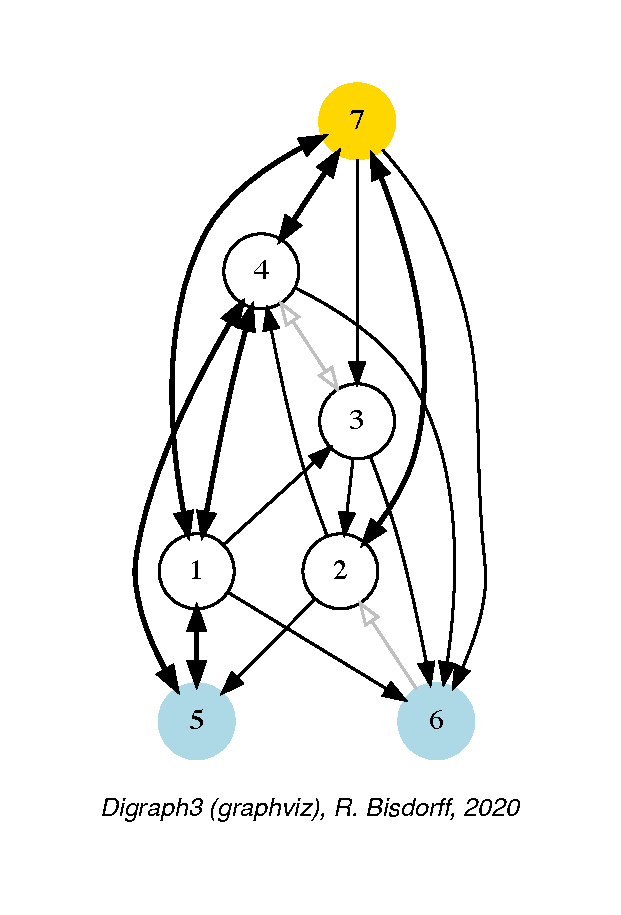
\includegraphics[height=6cm]{Figures/2-4-tutRandValDigraph_border.pdf}\hfill
  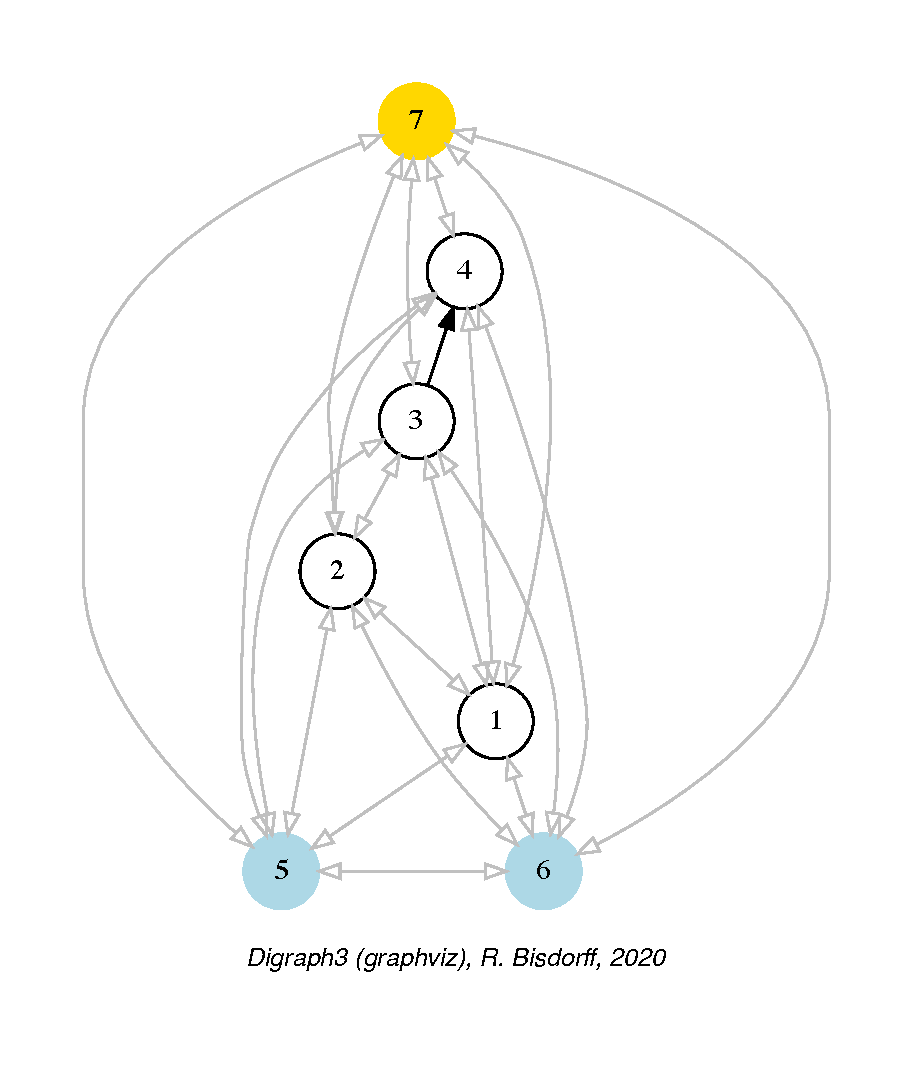
\includegraphics[height=6cm]{Figures/2-4-tutRandValDigraph_inner.pdf}\hfill
\caption{Border and inner part of the tutorial random valuation digraph \texttt{rdg}}
\label{fig:2.4}       % Give a unique label
\end{figure}

\section{Fusion by epistemic disjunction}
\label{sec:2.5}

We may recover object \texttt{rdg} from both partial objects \texttt{asymDg} and \texttt{symDg}, or as well from the border \texttt{bg} and the inner part \texttt{ig}, with a \emph{bipolar fusion} operator, also called \emph{epistemic disjunction}, available via the \texttt{FusionDigraph}\index{FusionDigraph@\texttt{FusionDigraph} class} class. 
\begin{lstlisting}[caption={Epistemic fusion of partial diagraphs},label=list:2.6]
>>> from digraphs import FusionDigraph
>>> fusDg = FusionDigraph(asymDg,symDg,operator='o-max')
>>> # fusDg = FusionDigraph(bg,ig,operator='o-max')
>>> fusDg.showRelationTable()
  * ---- Relation Table -----
   r(xSy) |  '1'    '2'   '3'  '4'   '5'    '6'  '7'	  
   -------|------------------------------------------
    '1'   |  0.00 -0.48  0.70  0.86  0.30  0.38  0.44	 
    '2'   | -0.22  0.00 -0.38  0.50  0.80 -0.54  0.02	 
    '3'   | -0.42  0.08  0.00  0.70 -0.56  0.84 -1.00	 
    '4'   |  0.44 -0.40 -0.62  0.00  0.04  0.66  0.76	 
    '5'   |  0.32 -0.48 -0.46  0.64  0.00 -0.22 -0.52	 
    '6'   | -0.84  0.00 -0.40 -0.96 -0.18  0.00 -0.22	 
    '7'   |  0.88  0.72  0.82  0.52 -0.84  0.04  0.00
\end{lstlisting}

The epistemic fusion operator \texttt{o-max} (see List.~\vref{list:2.6} Line 2) is defined as follows:
\begin{definition}[Disjunctive epistemic fusion operator \texttt{o-max}]\label{def:disjunctiveFusion}

\noindent Let $r$ and $r'$ characterise two bipolar-valued epistemic situations:
\begin{itemize}[leftmargin=0.5cm,rightmargin=0.5cm,nosep]
\item \texttt{o-max}$(r, r')$ = $\max(r, r' )$ when both $r$ and $r'$ are more or less valid or indeterminate;
\item \texttt{o-max}$(r, r')$ = $\min(r, r' )$ when both $r$ and $r'$ are more or less invalid or indeterminate;
\item \texttt{o-max}$(r, r')$ = $0.0$, i.e. indeterminate otherwise.
\end{itemize}
\end{definition}

Mind that the \texttt{o-max} operator, like a mean operator, is \emph{not associative} when more than 2 operands are given. In order to make the \texttt{o-max} fusion univocal, the following rule is applied: --first, all positive and negative terms are separately aggregated, --then the \texttt{o-max} fusion is applied on both aggregates.

\section{Dual, converse and codual digraphs}
\label{sec:2.6}

We may as readily compute the \emph{dual}\index{DualDigraph@\texttt{DualDigraph} class} (negated relation \footnote{Not to be confused with the dual graph of a plane graph $g$ that has a vertex for each face of $g$. Here we mean the \emph{less than} (strict converse) relation corresponding to a \emph{greater or equal} relation, or the \emph{less than or equal} relation corresponding to a (strict) \emph{better than} relation.}), the \emph{converse}\index{ConverseDigraph@\texttt{ConverseDigraph} class} (transposed relation) and the \emph{codual}\index{CoDualDigraph@\texttt{CoDualDigraph} class} (transposed and negated relation) of the digraph instance \texttt{rdg}. 
\begin{lstlisting}[caption={Computing associated dual, converse and codual digraphs},label=list:2.7]
>>> from digraphs import\
...          DualDigraph, ConverseDigraph, CoDualDigraph
>>> # dual of rdg
>>> ddg = DualDigraph(rdg)
>>> ddg.showRelationTable()
    -r(xSy) |  '1'    '2'   '3'  '4'   '5'    '6'  '7'	  
    --------|------------------------------------------
    '1 '    |  0.00  0.48 -0.70 -0.86 -0.30 -0.38 -0.44	 
    '2'     |  0.22  0.00  0.38 -0.50  0.80  0.54 -0.02	 
    '3'     |  0.42  0.08  0.00 -0.70  0.56 -0.84  1.00	 
    '4'     | -0.44  0.40  0.62  0.00 -0.04 -0.66 -0.76	 
    '5'     | -0.32  0.48  0.46 -0.64  0.00  0.22  0.52	 
    '6'     |  0.84  0.00  0.40  0.96  0.18  0.00  0.22	 
    '7'     |  0.88 -0.72 -0.82 -0.52  0.84 -0.04  0.00
>>> # converse of rdg
>>> cdg = ConverseDigraph(rdg)
>>> cdg.showRelationTable()
    * ---- Relation Table -----
     r(ySx) |  '1'    '2'   '3'   '4'   '5'   '6'   '7'	  
    --------|------------------------------------------
    '1'     |  0.00 -0.22 -0.42  0.44  0.32 -0.84  0.88	 
    '2'     | -0.48  0.00  0.08 -0.40 -0.48  0.00  0.72	 
    '3'     |  0.70 -0.38  0.00 -0.62 -0.46 -0.40  0.82	 
    '4'     |  0.86  0.50  0.70  0.00  0.64 -0.96  0.52	 
    '5'     |  0.30  0.80 -0.56  0.04  0.00 -0.18 -0.84	 
    '6'     |  0.38 -0.54  0.84  0.66 -0.22  0.00  0.04	 
    '7'     |  0.44  0.02 -1.00  0.76 -0.52 -0.22  0.00	 
>>> # codual of rdg
>>> cddg = CoDualDigraph(rdg)
>>> cddg.showRelationTable()
    * ---- Relation Table -----
    -r(ySx) |  '1'    '2'   '3'   '4'   '5'   '6'   '7'	    
    --------|------------------------------------------
    '1'     |  0.00  0.22  0.42 -0.44 -0.32  0.84 -0.88	 
    '2'     |  0.48  0.00 -0.08  0.40  0.48  0.00 -0.72	 
    '3'     | -0.70  0.38  0.00  0.62  0.46  0.40 -0.82	 
    '4'     | -0.86 -0.50 -0.70  0.00 -0.64  0.96 -0.52	 
    '5'     | -0.30 -0.80  0.56 -0.04  0.00  0.18  0.84	 
    '6'     | -0.38  0.54 -0.84 -0.66  0.22  0.00 -0.04	 
    '7'     | -0.44 -0.02  1.00 -0.76  0.52  0.22  0.00	 
\end{lstlisting}

Computing the \emph{dual}, respectively the \emph{converse} of a digraph, may also be done with prefixing the \texttt{\_\_neg\_\_} ($-$) or the \texttt{\_\_invert\_\_} ($\sim$) operator. The \emph{codual} of a \texttt{Digraph} object may, hence, as well be computed with a \emph{composition} (in either order) of both operations.
\begin{lstlisting}[caption={Computing the dual, the converse and the codual of a digraph},label=list:2.8]
>>> ddg = -rdg   # dual of rdg
>>> cdg = ~rdg   # converse of rdg
>>> cddg = ~(-rdg) # = -(~(rdg) codual of rdg
>>> (-(~rdg)).showRelationTable()
  * ---- Relation Table -----
   -r(ySx) |  '1'    '2'   '3'   '4'   '5'   '6'   '7'	    
   --------|------------------------------------------
   '1'     |  0.00  0.22  0.42 -0.44 -0.32  0.84 -0.88	 
   '2'     |  0.48  0.00 -0.08  0.40  0.48  0.00 -0.72	 
   '3'     | -0.70  0.38  0.00  0.62  0.46  0.40 -0.82	 
   '4'     | -0.86 -0.50 -0.70  0.00 -0.64  0.96 -0.52	 
   '5'     | -0.30 -0.80  0.56 -0.04  0.00  0.18  0.84	 
   '6'     | -0.38  0.54 -0.84 -0.66  0.22  0.00 -0.04	 
   '7'     | -0.44 -0.02  1.00 -0.76  0.52  0.22  0.00	 
\end{lstlisting}
  
\section{Symmetric and transitive closures}
\label{sec:2.7}

Symmetric and transitive closures, by default in-site methods, are also available (see Fig.~\vref{fig:2.5})\index{closeSymmetric@\texttt{closeSymmetric()}}\index{closeTransitive@\texttt{closeTransitive()}}. Note that it is a good idea, before going ahead with these in-site operations, who irreversibly modify the original \texttt{rdg} object, to previously make a backup version of \texttt{rdg}. The simplest storage method, always provided by the generic \texttt{Digraph.save()} method, writes out in a named file the python content of the Digraph object in string representation (see Sec.~\vref{sec:1.3}).
\begin{lstlisting}[caption={Symmeric and transitive closures},label=list:2.9]
>>> rdg.save('tutRandValDigraph')
>>> rdg.closeSymmetric(InSite=True)
>>> rdg.closeTransitive(InSite=True)
>>> rdg.exportGraphViz('strongComponents')
\end{lstlisting}
\begin{figure}[h]
\sidecaption[t]
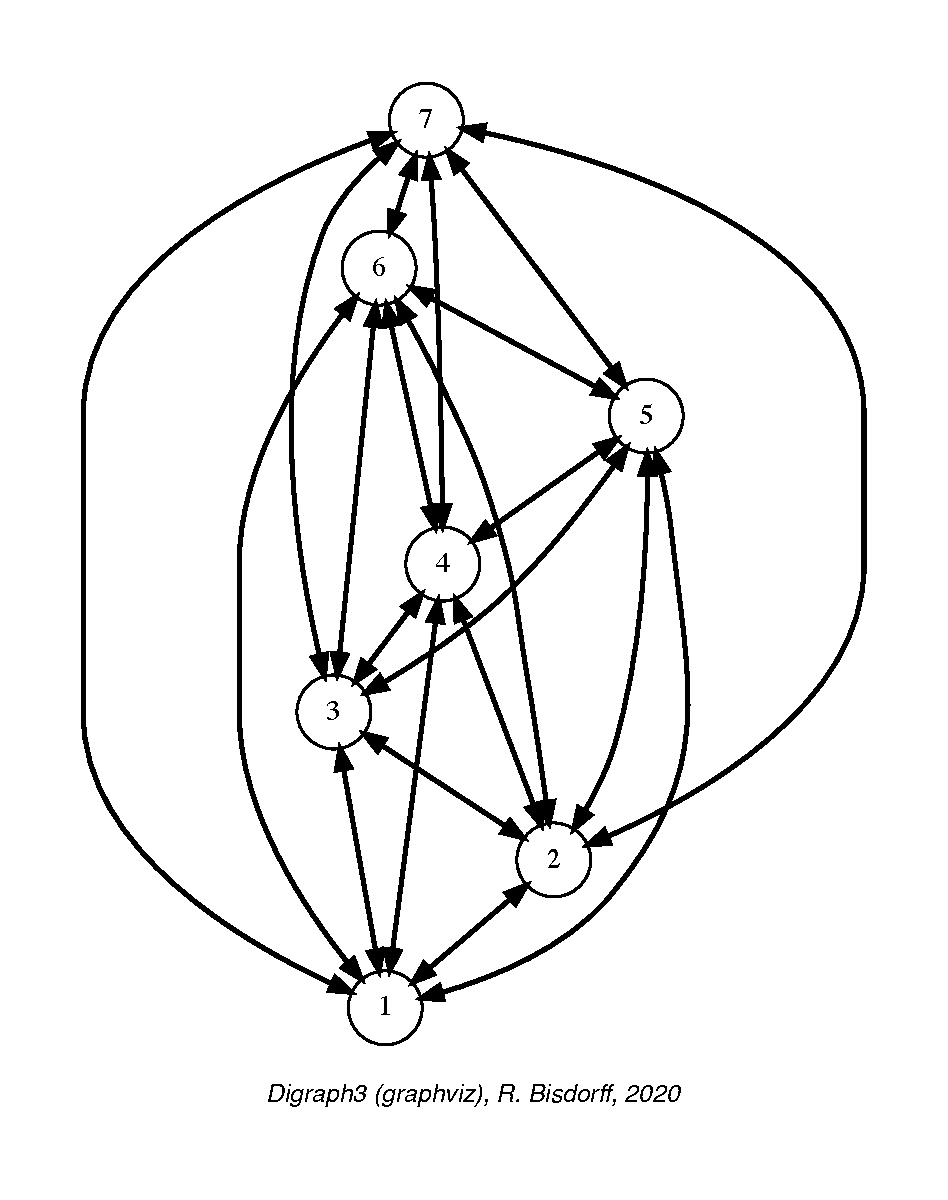
\includegraphics[width=6cm]{Figures/2-5-strongComponents.pdf}
\caption{Symmetric and transitive closure of the tutorial random valuation digraph $rdg$.}
\label{fig:2.5}       % Give a unique label
\end{figure}

The \texttt{closeSymmetric()}\index{closeSymmetric@\texttt{closeSymmetric()}} method (see List.~\vref{list:2.9} Line 2), of complexity $O(n^2)$ where $n$ denotes the digraph's order, changes, on the one hand, all single pairwise links it may detect into double links by operating a disjunction of the pairwise relations. On the other hand, the \texttt{closeTransitive()}\index{closeTransitive@\texttt{closeTransitive()}}  method (see Line 3), implements the \emph{Roy-Warshall} transitive closure algorithm of complexity $O(n^3)$ \index{Roy@\textsl{B. Roy}} \index{warshall@\textsl{S. Warshall}} (\citealp{ROY-1959} and \citealp{WAR-1962}).

The same \texttt{closeTransitive()} with a \texttt{Reverse = True} flag may be readily used for eliminating all transitive arcs from a transitive digraph instance. We make usage of this feature when drawing Hasse diagrams of \texttt{TransitiveDigraph}\index{TransitiveDigraph@\texttt{TransitiveDigraph} class} objects.

\section{Strong components}
\label{sec:2.8}

As the original digraph \texttt{rdg} was connected (see above the result of the showShort() command), both the symmetric and the transitive closures operated together, will necessarily produce a single strong component, i.e. a \textbf{complete} digraph. We may sometimes wish to collapse all strong components in a given digraph and construct the so \emph{collapsed} digraph. Using the \texttt{StrongComponentsCollapsedDigraph} constructor \index{StrongComponentsCollapsedDigraph@\texttt{StrongComponentsCollapsedDigraph} class} here will render a single hyper-node gathering all the original nodes (see Line 7 below).
\begin{lstlisting}[caption={Computing the strong components in a digraph},label=list:2.10]
>>> from digraphs import StrongComponentsCollapsedDigraph
>>> sc = StrongComponentsCollapsedDigraph(rdg)
>>> sc.showAll()
  *----- show detail -----*
   Digraph          : tutRandValDigraph_Scc
  *---- Actions ----*
    ['_7_1_2_6_5_3_4_']
  *---- Relation Table -----
      S     |  'Scc_1'	  
     -------|---------
     'Scc_1' |  0.00
  *---- strong Components ----*
   short 	 content
   'Scc_1' 	 '_7_1_2_6_5_3_4_'
  *---- Neighborhoods ----*
   Gamma     :
   'frozenset({'7','1','2','6','5','3','4'})':
                     in => set(), out => set()
   Not Gamma :
   'frozenset({'7','1','2','6','5','3','4'})':
                     in => set(), out => set()
\end{lstlisting}
  
\section{CSV storage}
\label{sec:2.9}

Sometimes it is required to exchange the graph valuation data in CSV format with a statistical package like \textbf{R}\footnote{\url{https://www.r-project.org/}}. For this purpose it is possible to export the digraph data into a CSV file. The valuation domain is hereby normalised by default to the range $[-1.0,1.0]$ and the diagonal is put by default to the minimal value $-1.0$.
\begin{lstlisting}
>>> rdg = Digraph('tutRandValDigraph')
>>> rdg.saveCSV('tutRandValDigraph')
  # content of file tutRandValDigraph.csv
  "d","1","2","3","4","5","6","7"
  "1",-1.0,0.48,-0.7,-0.86,-0.3,-0.38,-0.44
  "2",0.22,-1.0,0.38,-0.5,-0.8,0.54,-0.02
  "3",0.42,-0.08,-1.0,-0.7,0.56,-0.84,1.0
  "4",-0.44,0.4,0.62,-1.0,-0.04,-0.66,-0.76
  "5",-0.32,0.48,0.46,-0.64,-1.0,0.22,0.52
  "6",0.84,0.0,0.4,0.96,0.18,-1.0,0.22
  "7",-0.88,-0.72,-0.82,-0.52,0.84,-0.04,-1.0
\end{lstlisting}
  
It is possible to reload a \texttt{Digraph} instance from its previously saved CSV file content.
\begin{lstlisting} 
>>> from digraphs import CSVDigraph   
>>> rdgcsv = CSVDigraph('tutRandValDigraph')
>>> rdgcsv.showRelationTable(ReflexiveTerms=False)
    * ---- Relation Table -----
    r(xSy) |   '1'   '2'   '3'   '4'   '5'   '6'   '7'	  
    -------|------------------------------------------------------------
    '1'    |   -   -0.48  0.70  0.86  0.30  0.38  0.44	 
    '2'    | -0.22   -   -0.38  0.50  0.80 -0.54  0.02	 
    '3'    | -0.42  0.08   -    0.70 -0.56  0.84 -1.00	 
    '4'    |  0.44 -0.40 -0.62   -    0.04  0.66  0.76	 
    '5'    |  0.32 -0.48 -0.46  0.64   -   -0.22 -0.52	 
    '6'    | -0.84  0.00 -0.40 -0.96 -0.18   -   -0.22	 
    '7'    |  0.88  0.72  0.82  0.52 -0.84  0.04   -
\end{lstlisting}
  
It is as well possible to show a coloured version of the valued relation table in a system browser window tab (see Fig.~\vref{fig:2.5}).
\begin{lstlisting}
>>> rdgcsv.showHTMLRelationTable(tableTitle="Tutorial random digraph")
\end{lstlisting}
 \begin{figure}[ht]
\sidecaption[t]
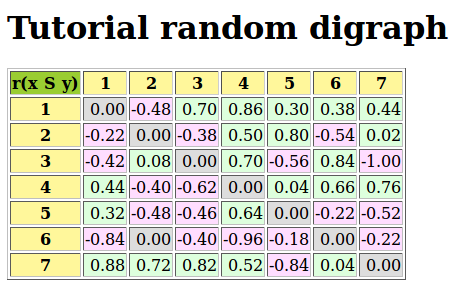
\includegraphics[width=7cm]{Figures/2-6-htmlTutorialDigraph.png}
\caption{The valued relation table shown in a browser window. Positive arcs are shown in green and negative arcs in red. Indeterminate --zero-valued-- links, like the reflexive diagonal ones or the link between node \texttt{'6'} and node \texttt{'2'}, are shown in gray}
\label{fig:2.6}       % Give a unique label
\end{figure}
 
\section{Complete, empty and indeterminate digraphs}
\label{sec:2.10}

Let us finally mention some special universal classes of digraphs that are readily available in the \texttt{digraphs} module\footnote{See \citealp{BIS-2021}}, like:
\begin{itemize}[nosep]
\item the \texttt{CompleteDigraph}\index{CompleteDigraph@\texttt{CompleteDigraph} class},
\item  the \texttt{EmptyDigraph}\index{EmptyDigraph@\texttt{EmptyDigraph} class} and
\item  the \texttt{IndeterminateDigraph}\index{IndeterminateDigraph@\texttt{IndeterminateDigraph} class} class,
\end{itemize}
who put all characteristic values respectively to the \emph{maximum}, the \emph{minimum} or the \emph{median} indeterminate characteristic value.
\begin{lstlisting}[caption={Complete, empty and indeterminate digraphs},label=list:2.11]
>>> from digraphs import CompleteDigraph,EmptyDigraph,\
...   			 IndeterminateDigraph
>>> # the empty digraph   
>>> e = EmptyDigraph(order=5)
>>> e.showRelationTable()
    * ---- Relation Table -----
      S   |    '1'    '2'    '3'    '4'	   '5'	  
    ---- -|-----------------------------------
    '1'   |  -1.00  -1.00  -1.00  -1.00	 -1.00	 
    '2'   |  -1.00  -1.00  -1.00  -1.00	 -1.00	 
    '3'   |  -1.00  -1.00  -1.00  -1.00	 -1.00	 
    '4'   |  -1.00  -1.00  -1.00  -1.00	 -1.00	 
    '5'   |  -1.00  -1.00  -1.00  -1.00	 -1.00
>>> e.showNeighborhoods() 
    Neighborhoods:
      Gamma     :
    '1': in => set(), out => set()
    '2': in => set(), out => set()
    '5': in => set(), out => set()
    '3': in => set(), out => set()
    '4': in => set(), out => set()
      Not Gamma :
    '1': in => {'2','4','5','3'}, out => {'2','4','5','3'}
    '2': in => {'1','4','5','3'}, out => {'1','4','5','3'}
    '5': in => {'1','2','4','3'}, out => {'1','2','4','3'}
    '3': in => {'1','2','4','5'}, out => {'1','2','4','5'}
    '4': in => {'1','2','5','3'}, out => {'1','2','5','3'}
>>> # the indeterminate digraph
>>> i = IndeterminateDigraph()
    * ---- Relation Table -----
      S   |   '1'   '2'	  '3'	'4'   '5'	  
    ------|------------------------------
    '1'   |  0.00  0.00	 0.00  0.00  0.00	 
    '2'   |  0.00  0.00	 0.00  0.00  0.00	 
    '3'   |  0.00  0.00	 0.00  0.00  0.00	 
    '4'   |  0.00  0.00	 0.00  0.00  0.00	 
    '5'   |  0.00  0.00	 0.00  0.00  0.00	 
>>> i.showNeighborhoods()
    Neighborhoods:
      Gamma     :
    '1': in => set(), out => set()
    '2': in => set(), out => set()
    '5': in => set(), out => set()
    '3': in => set(), out => set()
    '4': in => set(), out => set()
      Not Gamma :
    '1': in => set(), out => set()
    '2': in => set(), out => set()
    '5': in => set(), out => set()
    '3': in => set(), out => set()
    '4': in => set(), out => set()
\end{lstlisting}

Mind the subtle difference between the neighbourhoods of an \emph{empty} and the neighbourhoods of an \emph{indeterminate} digraph instance. In the first kind, the neighbourhoods are known to be completely \emph{empty}  (see List.~\vref{list:2.11} Lines 22-27) whereas, in the latter, \emph{nothing is known} about the actual neighbourhoods of the nodes  (see Lines 46-51). These two cases illustrate why in the case of \emph{bipolar-valued} digraphs, we may sometimes need both a \texttt{gamma} \textbf{and} a \texttt{notGamma} attribute.

\vspace{1cm}
In the following Chapter~\ref{sec:3}  we introduce the main formal object of this book, namely \emph{bipolar-valued outranking} digraphs.

%%%%%%%%%%%%%%%%%%%%%%%%%%%%%%%%%%%%
\phantomsection
\addcontentsline{toc}{section}{Notes}
\section*{Notes}

It is \emph{D. Bouyssou} \index{Bouyssou@\emph{D. Bouyssou}} who first suggested us end of the nineties, when we started to work in Prolog on the computation of digraph kernels with finite domain constraint solvers, that the $50\%$ criteria significance majority was a special value to be carefully taken into account. The converging solution vectors of the fixpoint kernel equations confirmed this special status of the $50\%$ majority (see Chap.~\ref{sec:17}). These early insights led to the seminal articles on bipolar-valued epistemic logic where we introduced split truth/falseness semantics for a multi-valued logical processing of fuzzy preference modelling \citep{BIS-2000,BIS-2002}. The characteristic valuation domain remained however the classical fuzzy $[0.0;1.0]$ valuation domain.

It is only in 2004, when we succeeded in assessing the stability of the outranking digraph when solely ordinal criteria significance weights are given, that it became clear and evident for us that the characteristic valuation domain had to be shifted to a bipolar $[-1.0;+1.0]$-valued domain \citep{BIS-2004a}. In this bipolar valuation domain, the $50\%$ majority thershold corresponds now to the median $0.0$ value, characterising with the correct zero value an epistemic indetermination --no knowledge-- situation. Furthermore, identifying truth and falseness by the sign of the characteristic values revealed itself to be very efficient not only from a computational point of view, but also from scientific and semiotical perspectives. A positive (resp. negative) characteristic value now attest a logically valid (resp. invalid) statement and a negative affirmation now corresponds to a positive refutation. Furthermore, the median zero value gives way to efficiently handling partial digraphs --like the border or the assymetric part of a digraph-- and, even more important from a practical decision making point of view, any missing data.

The bipolar $[-1.0;+1.0]$-valued characteritisc domain opened so the way to important new operations and concepts, like the disjunctive epistemic fusion operation seen in Section~\vref{sec:2.5} that confers the outranking digraph a logically and epistemically sound definition \citep{BIS-2013}. \Kendall 's ordinal correlation index could be extended to a bipolar-valued relational equivalence index between digraphs \citep{BIS-2012a}. Making usage of the bipolar-valued Gaussian error function naturally led to defining a bipolar-valued likelihood function, where a positive (resp. negative) value gives the likelihood of an affirmation (resp. a refutation) \citep{BIS-2014}.      

%%%%%%% The chapter bibliography
%\normallatexbib
%\clearpage
%\phantomsection
%\addcontentsline{toc}{section}{Chapter Bibliograhy}
\bibliographystyle{spbasic}
%\typeout{}
\bibliography{03-backMatters/reference}
%\input{02-mainMatters/02-chapterDigraphs.bbl}
\chapter{Working with outranking digraphs}
\label{sec:3}

\abstract*{ In this chapter, we introduce the main formal object of this book, namely the bipolar-valued outranking digraph. With a randomly generated multiple criteria performance tableau, we construct the corresponding bipolar-valued outranking relation from pairwise comparisons. The resulting bipolar-valued outranking characteristics may be recoded. Finally, the codual outranking digraph gives us the associated strict outranking relation.}

\begin{quotation}
``\emph{The rule for the combination of independent concurrent arguments takes a very simple form when expressed in terms of the intensity of belief ... It is this: Take the sum of all the feelings of belief which would be produced separately by all the arguments pro, subtract from that the similar sum for arguments con, and the remainder is the feeling of belief which ought to have the whole. This is a proceeding which men often resort to, under the name of balancing reasons.}'' -- C.S. Peirce, The probability of induction (1878)
\end{quotation}
\vspace{1cm}

\abstract{ In this chapter, we introduce the main formal object of this book, namely the bipolar-valued outranking digraph. With a randomly generated multiple criteria performance tableau, we construct the corresponding bipolar-valued outranking relation from pairwise comparisons. The resulting bipolar-valued outranking characteristics may be recoded. Finally, the codual outranking digraph gives us the associated strict outranking relation.}


\section{The hybrid outranking digraph model}
\label{sec:3.1}

In the \texttt{outrankingDigraphs} module\index{outrankingDigraphs@\texttt{outrankingDigraphs} module}, the \texttt{BipolarOutrankingDigraph}\index{BipolarOutrankingDigraph@\texttt{BipolarOutrankingDigraph} class} class provides our standard \emph{outranking digraph} constructor. Such an instance represents a \emph{hybrid} object of both the \texttt{PerformanceTableau} type \emph{and} the \texttt{Outran\-kingDigraph} type \citep{BIS-2021b}.

A given \texttt{BipolarOutrankingDigraph} object contains hence always at least the following attributes:
\begin{enumerate}[topsep=3pt,partopsep=0pt]
\item \texttt{actions}: an ordered dictionary describing the potential decision actions or alternatives with \texttt{name} and \texttt{comment} attributes,
\item \texttt{objectives}: a possibly empty ordered dictionary of decision objectives with \texttt{name} and \texttt{comment} attributes, describing the multiple preference dimensions involved in the decision problem, 
\item \texttt{criteria}: an ordered dictionary of performance criteria, i.e. \emph{preferentially independent} and \emph{non-redundant} decimal-valued evaluation functions used for assessng the performance of each potential decision action with respect to a decision objective,
\item \texttt{evaluation}: a double dictionary gathering performance evaluations for each decision alternative on each criterion function. 
\item \texttt{valuationdomain}: a dictionary with three entries: the minimum ($-1.0$, \emph{certainly outranked}), the median ($0.0$, \emph{indeterminate}) and the maximum characteristic value ($+1.0$, \emph{certainly outranking}),
\item \texttt{relation}: a double dictionary defined on the Cartesian product of the set of decision alternatives capturing the credibility of the pairwise \emph{outranking situation} computed on the basis of the performance differences observed between couples of decision alternatives on the given family of criteria functions.   
\end{enumerate}

Let us consider, for instance, a random bipolar-valued outranking digraph with seven decision actions denoted \texttt{a1}, \texttt{a2}, ..., \texttt{a7}. We need therefore, first, to generate in Listing~\vref{list:3.1} a corresponding random performance tableau.
\begin{lstlisting}[caption={Generating a random performance tableau.},label=list:3.1]
>>> from perfTabs import RandomPerformanceTableau
>>> pt = RandomPerformanceTableau(numberOfActions=7,\
...                               seed=100)   
>>> pt
   *------- PerformanceTableau instance description ------*
    Instance class     : RandomPerformanceTableau
    Seed               : 100
    Instance name      : randomperftab
    Actions            : 7
    Criteria           : 7
    NaN proportion (%) : 6.1
>>> pt.showActions()
  *----- show digraphs actions --------------*
   key:  a1
    name:       action 1
    comment:    RandomPerformanceTableau() generated.
   key:  a2
    name:       action 2
    comment:    RandomPerformanceTableau() generated.
     ...
     ...
   key:  a7
    name:       action 7
    comment:    RandomPerformanceTableau() generated.
\end{lstlisting}

In this example we consider a family of seven \emph{equisignificant} cardinal \emph{criteria functions} \texttt{g1}, \texttt{g2}, ..., \texttt{g7}, measuring the performance of each alternative on a rational scale from $0.0$ (worst) to $100.00$ (best). In order to capture the evaluation procedures' potential \emph{uncertainty} and \emph{imprecision}, each criterion function \texttt{g1} to \texttt{g7} admits three performance \emph{discrimination thresholds} of $2.5$, $5.0$ and $80.0$ pts for warranting respectively any \emph{indifference}, \emph{preference} or \emph{considerable performance difference} situation.
\begin{lstlisting}[caption={Inspecting the performance criteria.},label=list:3.2]
>>> pt.showCriteria()
  *----  criteria -----*
   g1 'RandomPerformanceTableau() instance'
     Scale = [0.0, 100.0]
     Weight = 1.0
     Threshold ind : 2.50 + 0.00x ; percentile: 4.76
     Threshold pref : 5.00 + 0.00x ; percentile: 9.52
     Threshold veto : 80.00 + 0.00x ; percentile: 95.24
   g2 'RandomPerformanceTableau() instance'
     Scale = [0.0, 100.0]
     Weight = 1.0
     Threshold ind : 2.50 + 0.00x ; percentile: 6.67
     Threshold pref : 5.00 + 0.00x ; percentile: 6.67
     Threshold veto : 80.00 + 0.00x ; percentile: 100.00
      ...
      ...
   g7 'RandomPerformanceTableau() instance'
     Scale = [0.0, 100.0]
     Weight = 1.0
     Threshold ind : 2.50 + 0.00x ; percentile: 0.00
     Threshold pref : 5.00 + 0.00x ; percentile: 4.76
     Threshold veto : 80.00 + 0.00x ; percentile: 100.00
\end{lstlisting}

On criteria function \texttt{g1} (see Lines 6-8 in List.~\vref{list:3.2}) we observe, for instance, about $5\%$ of \emph{indifference} situations, about $90\%$ of \emph{preference} situations and about $5\%$ of \emph{considerable} performance difference situations.

The individual \emph{performance evaluation} of all decision alternative on each criterion are gathered in a \emph{performance table}.\index{showPerformanceTableau@\texttt{showPerformanceTableau()}}
\begin{lstlisting}[caption={Inspecting the performance evaluations},label=list:3.3]
>>> pt.showPerformanceTableau()
    *----  performance tableau -----*
     criteria |  'a1'  'a2'  'a3'  'a4'  'a5'  'a6'  'a7'   
     ---------|------------------------------------------
      'g1'    |  15.2  44.5  57.9  58.0  24.2  29.1  96.6  
      'g2'    |  82.3  43.9   NA   35.8  29.1  34.8  62.2  
      'g3'    |  44.2  19.1  27.7  41.5  22.4  21.5  56.9  
      'g4'    |  46.4  16.2  21.5  51.2  77.0  39.4  32.1  
      'g5'    |  47.7  14.8  79.7  67.5   NA   90.7  80.2  
      'g6'    |  69.6  45.5  22.0  33.8  31.8   NA   48.8  
      'g7'    |  82.9  41.7  12.8  21.9  75.7  15.4   6.0  
\end{lstlisting}

It is noteworthy to mention the three \emph{missing data} (\texttt{NA}) cases: action \texttt{a3} is missing, for instance, an evaluation on criterion \texttt{g2} (see Line 6 in List.~\vref{list:3.3}).
    
\section{The bipolar-valued outranking digraph}
\label{sec:3.2}

Given the previous random performance tableau \texttt{pt}, the \texttt{BipolarOutranking\-Digraph}\index{BipolarOutrankingDigraph@\texttt{BipolarOutrankingDigraph}} class constructor computes the corresponding \emph{bipolar-valued outranking digraph}. 
\begin{lstlisting}[caption={Example of random bipolar-valued outranking digraph.},label=list:3.4]
>>> from outrankingDigraphs import \
...                       BipolarOutrankingDigraph
>>> odg = BipolarOutrankingDigraph(pt)
>>> odg
  *------- Object instance description ------*
   Instance class       : BipolarOutrankingDigraph
   Instance name        : rel_randomperftab
   Actions              : 7
   Criteria             : 7
   Size                 : 20
   Determinateness (%)  : 63.27
   Valuation domain     : [-1.00;1.00]
   Attributes           : [
        'name', 'actions', 
	'criteria', 'evaluation', 'NA',
	'valuationdomain', 'relation', 
	'order', 'gamma', 'notGamma', ...
	]
\end{lstlisting}

The resulting digraph contains 20 positive (valid) outranking relations. And, the mean majority criteria significance support of all the pairwise outranking situations is $63.3\%$ (see Lines 9-10 in List.~\vref{list:3.4}).

We may inspect the complete $[-1.0,+1.0]$-valued adjacency table with the \texttt{showRelationTable()} method().\index{showRelationTable@\texttt{showRelationTable()}}
\begin{lstlisting}[caption={Inspecting the valued adjacency table.},label=list:3.5]
>>> odg.showRelationTable()
  * ---- Relation Table -----
   r(x,y)|  'a1'   'a2'   'a3'   'a4'   'a5'   'a6'   'a7'   
   ------|-------------------------------------------------
    'a1' | +1.00  +0.71  +0.29  +0.29  +0.29  +0.29  +0.00  
    'a2' | -0.71  +1.00  -0.29  -0.14  +0.14  +0.29  -0.57  
    'a3' | -0.29  +0.29  +1.00  -0.29  -0.14  +0.00  -0.29  
    'a4' | +0.00  +0.14  +0.57  +1.00  +0.29  +0.57  -0.43  
    'a5' | -0.29  +0.00  +0.14  +0.00  +1.00  +0.29  -0.29  
    'a6' | -0.29  +0.00  +0.14  -0.29  +0.14  +1.00  +0.00  
    'a7' | +0.00  +0.71  +0.57  +0.43  +0.29  +0.00  +1.00  
   Valuation domain: [-1.0; 1.0]
\end{lstlisting}

The \texttt{BipolarOutrankingDigraph}\index{BipolarOutrankingDigraph@\texttt{BipolarOutrankingDigraph}} class constructor computes from the given performance tableau $pt$ the characteristic value $r(x \succsim y)$ of a \emph{pairwise outranking} relation $x\, \succsim \,y$ in a default \emph{valuation domain} $[-1.0,+1.0]$ with the {\em median\/} value $0.0$ acting as \emph{indeterminate} characteristic value\footnote{See Definition~\vref{def:3.1} \citep{BIS-2013}}. 

\begin{definition}[Semantics of the bipolar-valued characteristic function $r$]\label{def:3.1}

\noindent The semantics of $r(x \succsim y)$ are the following:
\begin{itemize}[nosep]
\item [a.] When $r(x \succsim y) > 0.0$, it is more {\em True\/} than {\em False\/} that $x$ \emph{outranks} $y$, i.e. alternative $x$ is ``\emph{at least as well evaluated as}'' alternative $y$ on a weighted majority of criteria {\bf and} there is no considerable negative performance difference observed in disfavour of $x$,
\item [b.] When $r(x \succsim y) < 0.0$, it is more {\em False\/} than {\em True\/} that $x$ \emph{outranks} $y$, i.e. alternative $x$ is {\bf not} ``\emph{at least as well evaluated as} alternative $y$ on a weighted majority of criteria than alternative $y$ {\bf and} there is no considerable positive performance difference observed in favour of $x$,
\item [c.] When $r(x \succsim y) = 0.0$, it is {\bf indeterminate} whether $x$ outranks $y$ or not.
\end{itemize}
\end{definition}

\section{Pairwise comparisons}
\label{sec:3.3}

From above given semantics, we notice in line 5 in Listing~\vref{list:3.5} that \texttt{a1} outranks \texttt{a2}: $r(a1 \succsim a2) + 0.71$), but not \texttt{a7}: $r(a1 \succsim a7) = 0.0$). In order to comprehend the characteristic values shown in the outranking relation table, we can inspect with the \texttt{showPairwiseComparison()} method\index{showPairwiseComparison@\texttt{showPairwiseComparison()}} the details of the pairwise multiple criteria comparison between, for instance, alternatives \texttt{a1} and \texttt{a2}.
\begin{lstlisting}[caption={Inspecting a pairwise multiple criteria comparison},label=list:3.6]
>>> odg.showPairwiseComparison('a1','a2')
  *------------  pairwise comparison ----*
   Comparing actions : (a1, a2)
   crit. wght. g(a1)  g(a2)   diff  | ind   pref    r() 
   -------------------------------  	 --------------------
    g1   1.00  15.17  44.51  -29.34 | 2.50  5.00   -1.00 
    g2   1.00  82.29  43.90  +38.39 | 2.50  5.00   +1.00 
    g3   1.00  44.23  19.10  +25.13 | 2.50  5.00   +1.00 
    g4   1.00  46.37  16.22  +30.15 | 2.50  5.00   +1.00 
    g5   1.00  47.67  14.81  +32.86 | 2.50  5.00   +1.00 
    g6   1.00  69.62  45.49  +24.13 | 2.50  5.00   +1.00 
    g7   1.00  82.88  41.66  +41.22 | 2.50  5.00   +1.00 
    Valuation in range: -7.00 to +7.00;          -------
       r(a1,a2): +5.00/7.00 = +0.71                +5.00
\end{lstlisting}

The outranking characteristic value $r(a1 \succsim a2)$ represents the relative \emph{majority margin} resulting from the difference between the significance weights of the criteria in favour and the significance weights of the criteria in disfavour of the statement that alternative \texttt{a1} is ``\emph{at least as well evaluated as}'' alternative \texttt{a2}. No considerable performance difference being observed, no polarising situation is triggered in this pairwise comparison.

Such a polarised situation is however observed when we compare the evaluations of alternatives \texttt{a1} and \texttt{a7} with the \texttt{showPairwiseOutrankings()} method. \index{showPairwiseoutrankings@\texttt{showPairwiseOutrankings()}}
\begin{lstlisting}[caption={Pairwise comparison with considerable performance difference},label=list:3.7,basicstyle=\ttfamily\scriptsize]
>>> odg.showPairwiseoutrankings('a1','a7')
  *------------  pairwise comparison ----*
   Comparing actions : (a1, a7)
   crit. wght. g(a1)  g(a7)   diff  | ind   pref    r()  |  v     veto
   -------------------------------   ------------------   -----------
    g1   1.00  15.17  96.58  -81.41 | 2.50  5.00   -1.00 | 80.00 -1.00
    g2   1.00  82.29  62.22  +20.07 | 2.50  5.00   +1.00 | 
    g3   1.00  44.23  56.90  -12.67 | 2.50  5.00   -1.00 | 
    g4   1.00  46.37  32.06  +14.31 | 2.50  5.00   +1.00 | 
    g5   1.00  47.67  80.16  -32.49 | 2.50  5.00   -1.00 | 
    g6   1.00  69.62  48.80  +20.82 | 2.50  5.00   +1.00 | 
    g7   1.00  82.88   6.05  +76.83 | 2.50  5.00   +1.00 | 
   ----------------------------------------
   Valuation in range: -7.00 to +7.00; r(x,y)= +1/7 => 0.0
  *------------  pairwise comparison ----*
   Comparing actions : (a1, a7)
   crit. wght. g(a7)  g(a1)   diff  | ind   pref    r()  |  v     veto
   -------------------------------   ------------------   -----------
    g1   1.00  96.58  15.17  +81.41 | 2.50  5.00   +1.00 | 80.00 +1.00
    g2   1.00  62.22  82.29  -20.07 | 2.50  5.00   -1.00 | 
    g3   1.00  56.90  44.23  +12.67 | 2.50  5.00   +1.00 | 
    g4   1.00  32.06  46.37  -14.31 | 2.50  5.00   -1.00 | 
    g5   1.00  80.16  47.67  +32.49 | 2.50  5.00   +1.00 | 
    g6   1.00  48.80  69.62  -20.82 | 2.50  5.00   -1.00 | 
    g7   1.00   6.05  82.88  -76.83 | 2.50  5.00   -1.00 | 
   ----------------------------------------
   Valuation in range: -7.00 to +7.00; r(x,y)= -1/7 => 0.0
\end{lstlisting}

This time, we observe a $(1/7 + 1)/2 = 57.1\%$ majority of criteria significance warranting a ``\emph{at least as well evaluated as}'' situation between alternative \texttt{a1} and alternative \texttt{a7}. Yet, we also observe a considerable \emph{negative} performance difference on criterion \texttt{g1} (see Line 6 in List.~\vref{list:3.7}). Both contradictory facts trigger eventually in Line 14 an \emph{indeterminate} outranking situation. The inverse polarisation effect appears when considering in Lines 19-25 the converse performance differences between alternative \texttt{a7} and alternative \texttt{a1}. The considerable better performing situation on criterion \texttt{g1} makes doubtful the otherwise ``\emph{not at least as well evaluated as}'' situation (see Lines 19 and 27).

Notice that the occurrence in a pairwise comparison of conjointly considerable positive and negative performance differences will also trigger an indeterminate outranking situation. When observing at the same time a positive (resp. negative) ``\emph{at least as well evaluated as}'' situation and one or more considerable positive (resp. negative) performance difference, the outranking situation gets validated (resp. invalidated) for certain \citep{BIS-2013}.

\section{Recoding the characteristic valuation domain}
\label{sec:3.4}

All outranking digraphs, being of root \texttt{Digraph} type, inherit the methods available under this latter class. The characteristic valuation domain of a digraph can, for instance, be recoded with the \texttt{recodeValuation()}\index{recodeValuation@\emph{recodeValuation()}} method to the \emph{integer} range $[-7,+7]$, i.e. plus or minus the total significance weights of the family of criteria considered in this example instance \texttt{odg}.
\begin{lstlisting}[caption={Recoding the digraph valuation},label=list:3.8]
>>> odg.recodeValuation(-7,+7)
>>> odg.valuationdomain['hasIntegerValuation'] = True
>>> Digraph.showRelationTable(odg,ReflexiveTerms=False)
  * ---- Relation Table -----
   r(x,y)  |  'a1'  'a2'  'a3'  'a4'  'a5'  'a6'  'a7'	  
  ---------|------------------------------------------
    'a1'   |    -    +5    +2    +2    +2    +2     0	 
    'a2'   |   -5     -    -1    -1    +1    +2    -4	 
    'a3'   |   -1    +2     -    -1    -1     0    -1	 
    'a4'   |    0    +1    +4     -    +2    +4    -3	 
    'a5'   |   -1     0    +1     0     -    +2    -1	 
    'a6'   |   -1     0    +1    -1    +1     -     0	 
    'a7'   |    0    +5    +4    +3    +2     0     -	 
    Valuation domain: [-7;+7]
\end{lstlisting}

Notice in Listing~\vref{list:3.8} that the self comparison characteristics $r(x \succsim x)$ may be ignored by setting the \texttt{ReflexiveTerms} Boolean parameter to \texttt{False}. Mind that the trivial reflexive terms of outranking relations are ignored in some of the \Digraph methods. 

\section{The strict outranking digraph}
\label{sec:3.5}

From theory we know that a bipolar-valued outranking digraph is \emph{weakly complete}, i.e. if $r(x \succsim y) < 0.0$ then $r(y \succsim x) \geq 0.0$. From this property follows that a bipolar-valued outranking digraph verifies the \emph{coduality principle}\index{coduality principle}: the \emph{dual}\footnote{Not to be confused with the dual graph of a plane graph $g$ that has a vertex for each face of $g$. Here we mean the \emph{less than} (strict converse) relation corresponding to a \emph{greater or equal} relation, or the \emph{less than or equal} relation corresponding to a (strict) \emph{better than} relation.} --strict negation-- of the \emph{converse} --inverse-- of the outranking relation $(x \succsim y)$ corresponds to its asymmetric \emph{strict outranking} part $(x \succnsim y)$  \citep{BIS-2013, ADT-L7}.

We may visualize the \emph{codual} (\emph{strict}) outranking digraph with a graphviz drawing \footnote{The \texttt{exportGraphViz()} method is depending on drawing tools from the graphviz software (https://graphviz.org/). On Linux Ubuntu or Debian you may try \texttt{sudo apt-get install graphviz} to install them. There are ready \emph{dmg} installers for Mac OSX.}.\index{graphviz}
\begin{lstlisting}
>>> cdodg = -(~odg)
>>> cdodg.exportGraphViz('codualOdg')
  *---- exporting a dot file for GraphViz tools ---------*
   Exporting to codualOdg.dot
   dot -Grankdir=BT -Tpng codualOdg.dot -o codualOdg.png
\end{lstlisting}
\begin{figure}[ht]
\sidecaption[t]
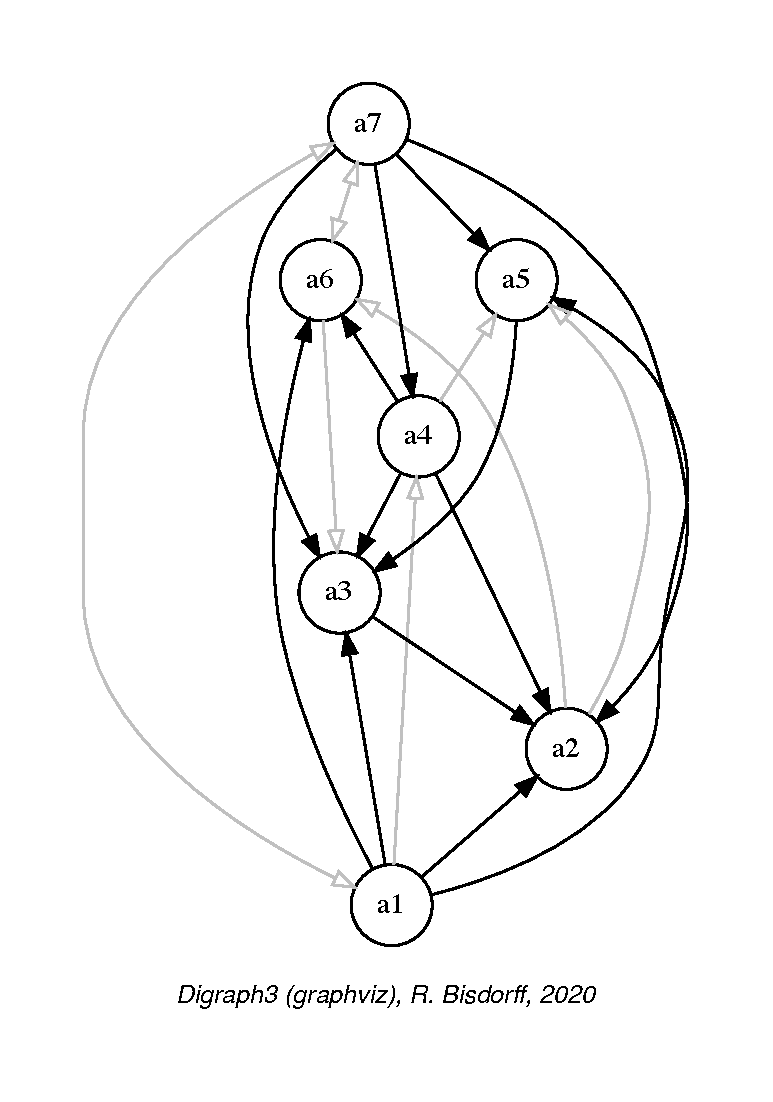
\includegraphics[width=5cm]{Figures/3-1-codualOdg.pdf}
\caption[The strict (codual) outranking digraph]{The strict (codual) outranking digraph. It becomes readily clear now from the picture that both alternatives \texttt{a1}  and \texttt{a7} are \emph{not outranked} by any other alternatives. Hence, \texttt{a1}  and \texttt{a7} appear as \emph{weak} \Condorcet winners and may be recommended as potential \emph{best} decision alternatives in this illustrative preference modelling example}
\label{fig:3.1}       % Give a unique label
\end{figure}
 
Many more tools for exploiting bipolar-valued outranking digraphs are available in the \Digraph resources \citep{BIS-2021b}.
\vspace{1cm}

In the methodological Part II, we present and discuss multiple criteria evaluation models and decision algorithms, like building a best choice recommendation, determining the winner of an election, computing linear rankings or quantile ratings with multiple incommensurable criteria.

%%%%%%%%%%%%%%%%%%%%%%%%%%%%%%%%%%%%
\phantomsection
\addcontentsline{toc}{section}{Notes}
\section*{Notes}

The seminal work on outranking digraphs goes back to the seventies and eighties when Bernard Roy \index{Roy@\textsl{B. Roy}} joined the just starting University Paris-Dauphine and founded there the '\emph{Laboratoire d’Analyse et de Modélisation de Systèmes pour l’Aide à la Décision}' (LAMSADE). The LAMSADE became the major site in the development of the outranking approach to multiple criteria decision aid. \citep*{ROY-1993}.

The ongoing success of the original \emph{outranking} concept stems from the fact that it is rooted in a sound pragmatism. The multiple criteria performance tableau, necessarily associated with a given outranking digraph, is indeed convincingly objective and meaningful \citep{ROY-1991}. And, ideas from social choice theory gave initially the insight that a pairwise voting mechanism à la \Condorcet could provide an order-statistical tool for aggregating a set of preference points of view into what M. Barbut\index{Barbut@\emph{M. Barbut}} called the \emph{central} \Condorcet point of view (\citealp{CON-1784} and \citealp{BAR-1980}); in fact the median of the multiple preference points of view, at minimal absolute \Kendall's\index{Kendall@\emph{M.G. Kendall}} ordinal correlation distance from all individual points of view (see Chap.~\ref{sec:16}).

Considering thus each performance criterion as a subset of unanimous voters and balancing the votes in favour against considerable counter-performances in disfavour gave eventually rise to the concept of \emph{outranking situation}, a distinctive feature of the Multiple Criteria Decision Aid approach \citep{BIS-2015}.  A modern definition would be : An alternative $x$ is said to \emph{outrank} alternative $y$ when – a \emph{significant majority} of criteria confirm that alternative $x$ has to be considered as \emph{at least as well evaluated as} an alternative $y$ (the \emph{concordance} argument); and – no discordant criterion opens to significant doubt the validity of the previous confirmation by revealing a considerable counter-performance of alternative $x$ compared to $y$ (the \emph{discordance} argument).

If the concordance argument was always well received, the discordance argument however, very confused in the beginning \citep{ROY-1966}, could only be handled in an epistemically correct and logically sound way by using a bipolar-valued epistemic logic (see Def.~\vref{def:3.1} and \citealp{BIS-2013}). The outranking situation had consequently to receive an explicit negative definition: An alternative $x$ is said to \emph{do not outrank} an alternative $y$ when – a \emph{significant majority} of criteria confirm that alternative $x$ has to be considered as \emph{not at least as well evaluated as} alternative $y$; and – no discordant criterion opens to significant doubt the validity of the previous confirmation by revealing a considerable \emph{better} performance of alternative $x$ compared to $y$.

Furthermore, the initial conjunctive aggregation of the concordance and discordance arguments had to be replaced by a disjunctive epistemic fusion operation, polarising in a logically and epistemically sound way the concordance with the discordance argument. This way, bipolar-valued outranking  digraphs gain two very useful properties from a measure theoretical perspective. They are \emph{weakly complete}; incomparability situations are no longer attested by the absence of positive outranking relations, but instead by epistemic indeterminateness. And they verify the \emph{coduality principle}: the negation of the epistemic ``\emph{at least as well evaluated as}'' situation corresponds formally to the strict converse epistemic ``\emph{less well evaluated than}'' situation.


%%%%%%% The chapter bibliography
%\normallatexbib
\clearpage
%\phantomsection
%\addcontentsline{toc}{section}{Chapter Bibliography}
%\chapter{Working with outranking digraphs}
\label{sec:3}

\abstract*{ In this chapter, we introduce the main formal object of this book, namely the bipolar-valued outranking digraph. With a randomly generated multiple criteria performance tableau, we construct the corresponding bipolar-valued outranking relation from pairwise comparisons. The resulting bipolar-valued outranking characteristics may be recoded. Finally, the codual outranking digraph gives us the associated strict outranking relation.}

\begin{quotation}
``\emph{The rule for the combination of independent concurrent arguments takes a very simple form when expressed in terms of the intensity of belief ... It is this: Take the sum of all the feelings of belief which would be produced separately by all the arguments pro, subtract from that the similar sum for arguments con, and the remainder is the feeling of belief which ought to have the whole. This is a proceeding which men often resort to, under the name of balancing reasons.}'' -- C.S. Peirce, The probability of induction (1878)
\end{quotation}
\vspace{1cm}

\abstract{ In this chapter, we introduce the main formal object of this book, namely the bipolar-valued outranking digraph. With a randomly generated multiple criteria performance tableau, we construct the corresponding bipolar-valued outranking relation from pairwise comparisons. The resulting bipolar-valued outranking characteristics may be recoded. Finally, the codual outranking digraph gives us the associated strict outranking relation.}


\section{The hybrid outranking digraph model}
\label{sec:3.1}

In the \texttt{outrankingDigraphs} module\index{outrankingDigraphs@\texttt{outrankingDigraphs} module}, the \texttt{BipolarOutrankingDigraph}\index{BipolarOutrankingDigraph@\texttt{BipolarOutrankingDigraph} class} class provides our standard \emph{outranking digraph} constructor. Such an instance represents a \emph{hybrid} object of both the \texttt{PerformanceTableau} type \emph{and} the \texttt{Outran\-kingDigraph} type \citep{BIS-2021b}.

A given \texttt{BipolarOutrankingDigraph} object contains hence always at least the following attributes:
\begin{enumerate}[topsep=3pt,partopsep=0pt]
\item \texttt{actions}: an ordered dictionary describing the potential decision actions or alternatives with \texttt{name} and \texttt{comment} attributes,
\item \texttt{objectives}: a possibly empty ordered dictionary of decision objectives with \texttt{name} and \texttt{comment} attributes, describing the multiple preference dimensions involved in the decision problem, 
\item \texttt{criteria}: an ordered dictionary of performance criteria, i.e. \emph{preferentially independent} and \emph{non-redundant} decimal-valued evaluation functions used for assessng the performance of each potential decision action with respect to a decision objective,
\item \texttt{evaluation}: a double dictionary gathering performance evaluations for each decision alternative on each criterion function. 
\item \texttt{valuationdomain}: a dictionary with three entries: the minimum ($-1.0$, \emph{certainly outranked}), the median ($0.0$, \emph{indeterminate}) and the maximum characteristic value ($+1.0$, \emph{certainly outranking}),
\item \texttt{relation}: a double dictionary defined on the Cartesian product of the set of decision alternatives capturing the credibility of the pairwise \emph{outranking situation} computed on the basis of the performance differences observed between couples of decision alternatives on the given family of criteria functions.   
\end{enumerate}

Let us consider, for instance, a random bipolar-valued outranking digraph with seven decision actions denoted \texttt{a1}, \texttt{a2}, ..., \texttt{a7}. We need therefore, first, to generate in Listing~\vref{list:3.1} a corresponding random performance tableau.
\begin{lstlisting}[caption={Generating a random performance tableau.},label=list:3.1]
>>> from perfTabs import RandomPerformanceTableau
>>> pt = RandomPerformanceTableau(numberOfActions=7,\
...                               seed=100)   
>>> pt
   *------- PerformanceTableau instance description ------*
    Instance class     : RandomPerformanceTableau
    Seed               : 100
    Instance name      : randomperftab
    Actions            : 7
    Criteria           : 7
    NaN proportion (%) : 6.1
>>> pt.showActions()
  *----- show digraphs actions --------------*
   key:  a1
    name:       action 1
    comment:    RandomPerformanceTableau() generated.
   key:  a2
    name:       action 2
    comment:    RandomPerformanceTableau() generated.
     ...
     ...
   key:  a7
    name:       action 7
    comment:    RandomPerformanceTableau() generated.
\end{lstlisting}

In this example we consider a family of seven \emph{equisignificant} cardinal \emph{criteria functions} \texttt{g1}, \texttt{g2}, ..., \texttt{g7}, measuring the performance of each alternative on a rational scale from $0.0$ (worst) to $100.00$ (best). In order to capture the evaluation procedures' potential \emph{uncertainty} and \emph{imprecision}, each criterion function \texttt{g1} to \texttt{g7} admits three performance \emph{discrimination thresholds} of $2.5$, $5.0$ and $80.0$ pts for warranting respectively any \emph{indifference}, \emph{preference} or \emph{considerable performance difference} situation.
\begin{lstlisting}[caption={Inspecting the performance criteria.},label=list:3.2]
>>> pt.showCriteria()
  *----  criteria -----*
   g1 'RandomPerformanceTableau() instance'
     Scale = [0.0, 100.0]
     Weight = 1.0
     Threshold ind : 2.50 + 0.00x ; percentile: 4.76
     Threshold pref : 5.00 + 0.00x ; percentile: 9.52
     Threshold veto : 80.00 + 0.00x ; percentile: 95.24
   g2 'RandomPerformanceTableau() instance'
     Scale = [0.0, 100.0]
     Weight = 1.0
     Threshold ind : 2.50 + 0.00x ; percentile: 6.67
     Threshold pref : 5.00 + 0.00x ; percentile: 6.67
     Threshold veto : 80.00 + 0.00x ; percentile: 100.00
      ...
      ...
   g7 'RandomPerformanceTableau() instance'
     Scale = [0.0, 100.0]
     Weight = 1.0
     Threshold ind : 2.50 + 0.00x ; percentile: 0.00
     Threshold pref : 5.00 + 0.00x ; percentile: 4.76
     Threshold veto : 80.00 + 0.00x ; percentile: 100.00
\end{lstlisting}

On criteria function \texttt{g1} (see Lines 6-8 in List.~\vref{list:3.2}) we observe, for instance, about $5\%$ of \emph{indifference} situations, about $90\%$ of \emph{preference} situations and about $5\%$ of \emph{considerable} performance difference situations.

The individual \emph{performance evaluation} of all decision alternative on each criterion are gathered in a \emph{performance table}.\index{showPerformanceTableau@\texttt{showPerformanceTableau()}}
\begin{lstlisting}[caption={Inspecting the performance evaluations},label=list:3.3]
>>> pt.showPerformanceTableau()
    *----  performance tableau -----*
     criteria |  'a1'  'a2'  'a3'  'a4'  'a5'  'a6'  'a7'   
     ---------|------------------------------------------
      'g1'    |  15.2  44.5  57.9  58.0  24.2  29.1  96.6  
      'g2'    |  82.3  43.9   NA   35.8  29.1  34.8  62.2  
      'g3'    |  44.2  19.1  27.7  41.5  22.4  21.5  56.9  
      'g4'    |  46.4  16.2  21.5  51.2  77.0  39.4  32.1  
      'g5'    |  47.7  14.8  79.7  67.5   NA   90.7  80.2  
      'g6'    |  69.6  45.5  22.0  33.8  31.8   NA   48.8  
      'g7'    |  82.9  41.7  12.8  21.9  75.7  15.4   6.0  
\end{lstlisting}

It is noteworthy to mention the three \emph{missing data} (\texttt{NA}) cases: action \texttt{a3} is missing, for instance, an evaluation on criterion \texttt{g2} (see Line 6 in List.~\vref{list:3.3}).
    
\section{The bipolar-valued outranking digraph}
\label{sec:3.2}

Given the previous random performance tableau \texttt{pt}, the \texttt{BipolarOutranking\-Digraph}\index{BipolarOutrankingDigraph@\texttt{BipolarOutrankingDigraph}} class constructor computes the corresponding \emph{bipolar-valued outranking digraph}. 
\begin{lstlisting}[caption={Example of random bipolar-valued outranking digraph.},label=list:3.4]
>>> from outrankingDigraphs import \
...                       BipolarOutrankingDigraph
>>> odg = BipolarOutrankingDigraph(pt)
>>> odg
  *------- Object instance description ------*
   Instance class       : BipolarOutrankingDigraph
   Instance name        : rel_randomperftab
   Actions              : 7
   Criteria             : 7
   Size                 : 20
   Determinateness (%)  : 63.27
   Valuation domain     : [-1.00;1.00]
   Attributes           : [
        'name', 'actions', 
	'criteria', 'evaluation', 'NA',
	'valuationdomain', 'relation', 
	'order', 'gamma', 'notGamma', ...
	]
\end{lstlisting}

The resulting digraph contains 20 positive (valid) outranking relations. And, the mean majority criteria significance support of all the pairwise outranking situations is $63.3\%$ (see Lines 9-10 in List.~\vref{list:3.4}).

We may inspect the complete $[-1.0,+1.0]$-valued adjacency table with the \texttt{showRelationTable()} method().\index{showRelationTable@\texttt{showRelationTable()}}
\begin{lstlisting}[caption={Inspecting the valued adjacency table.},label=list:3.5]
>>> odg.showRelationTable()
  * ---- Relation Table -----
   r(x,y)|  'a1'   'a2'   'a3'   'a4'   'a5'   'a6'   'a7'   
   ------|-------------------------------------------------
    'a1' | +1.00  +0.71  +0.29  +0.29  +0.29  +0.29  +0.00  
    'a2' | -0.71  +1.00  -0.29  -0.14  +0.14  +0.29  -0.57  
    'a3' | -0.29  +0.29  +1.00  -0.29  -0.14  +0.00  -0.29  
    'a4' | +0.00  +0.14  +0.57  +1.00  +0.29  +0.57  -0.43  
    'a5' | -0.29  +0.00  +0.14  +0.00  +1.00  +0.29  -0.29  
    'a6' | -0.29  +0.00  +0.14  -0.29  +0.14  +1.00  +0.00  
    'a7' | +0.00  +0.71  +0.57  +0.43  +0.29  +0.00  +1.00  
   Valuation domain: [-1.0; 1.0]
\end{lstlisting}

The \texttt{BipolarOutrankingDigraph}\index{BipolarOutrankingDigraph@\texttt{BipolarOutrankingDigraph}} class constructor computes from the given performance tableau $pt$ the characteristic value $r(x \succsim y)$ of a \emph{pairwise outranking} relation $x\, \succsim \,y$ in a default \emph{valuation domain} $[-1.0,+1.0]$ with the {\em median\/} value $0.0$ acting as \emph{indeterminate} characteristic value\footnote{See Definition~\vref{def:3.1} \citep{BIS-2013}}. 

\begin{definition}[Semantics of the bipolar-valued characteristic function $r$]\label{def:3.1}

\noindent The semantics of $r(x \succsim y)$ are the following:
\begin{itemize}[nosep]
\item [a.] When $r(x \succsim y) > 0.0$, it is more {\em True\/} than {\em False\/} that $x$ \emph{outranks} $y$, i.e. alternative $x$ is ``\emph{at least as well evaluated as}'' alternative $y$ on a weighted majority of criteria {\bf and} there is no considerable negative performance difference observed in disfavour of $x$,
\item [b.] When $r(x \succsim y) < 0.0$, it is more {\em False\/} than {\em True\/} that $x$ \emph{outranks} $y$, i.e. alternative $x$ is {\bf not} ``\emph{at least as well evaluated as} alternative $y$ on a weighted majority of criteria than alternative $y$ {\bf and} there is no considerable positive performance difference observed in favour of $x$,
\item [c.] When $r(x \succsim y) = 0.0$, it is {\bf indeterminate} whether $x$ outranks $y$ or not.
\end{itemize}
\end{definition}

\section{Pairwise comparisons}
\label{sec:3.3}

From above given semantics, we notice in line 5 in Listing~\vref{list:3.5} that \texttt{a1} outranks \texttt{a2}: $r(a1 \succsim a2) + 0.71$), but not \texttt{a7}: $r(a1 \succsim a7) = 0.0$). In order to comprehend the characteristic values shown in the outranking relation table, we can inspect with the \texttt{showPairwiseComparison()} method\index{showPairwiseComparison@\texttt{showPairwiseComparison()}} the details of the pairwise multiple criteria comparison between, for instance, alternatives \texttt{a1} and \texttt{a2}.
\begin{lstlisting}[caption={Inspecting a pairwise multiple criteria comparison},label=list:3.6]
>>> odg.showPairwiseComparison('a1','a2')
  *------------  pairwise comparison ----*
   Comparing actions : (a1, a2)
   crit. wght. g(a1)  g(a2)   diff  | ind   pref    r() 
   -------------------------------  	 --------------------
    g1   1.00  15.17  44.51  -29.34 | 2.50  5.00   -1.00 
    g2   1.00  82.29  43.90  +38.39 | 2.50  5.00   +1.00 
    g3   1.00  44.23  19.10  +25.13 | 2.50  5.00   +1.00 
    g4   1.00  46.37  16.22  +30.15 | 2.50  5.00   +1.00 
    g5   1.00  47.67  14.81  +32.86 | 2.50  5.00   +1.00 
    g6   1.00  69.62  45.49  +24.13 | 2.50  5.00   +1.00 
    g7   1.00  82.88  41.66  +41.22 | 2.50  5.00   +1.00 
    Valuation in range: -7.00 to +7.00;          -------
       r(a1,a2): +5.00/7.00 = +0.71                +5.00
\end{lstlisting}

The outranking characteristic value $r(a1 \succsim a2)$ represents the relative \emph{majority margin} resulting from the difference between the significance weights of the criteria in favour and the significance weights of the criteria in disfavour of the statement that alternative \texttt{a1} is ``\emph{at least as well evaluated as}'' alternative \texttt{a2}. No considerable performance difference being observed, no polarising situation is triggered in this pairwise comparison.

Such a polarised situation is however observed when we compare the evaluations of alternatives \texttt{a1} and \texttt{a7} with the \texttt{showPairwiseOutrankings()} method. \index{showPairwiseoutrankings@\texttt{showPairwiseOutrankings()}}
\begin{lstlisting}[caption={Pairwise comparison with considerable performance difference},label=list:3.7,basicstyle=\ttfamily\scriptsize]
>>> odg.showPairwiseoutrankings('a1','a7')
  *------------  pairwise comparison ----*
   Comparing actions : (a1, a7)
   crit. wght. g(a1)  g(a7)   diff  | ind   pref    r()  |  v     veto
   -------------------------------   ------------------   -----------
    g1   1.00  15.17  96.58  -81.41 | 2.50  5.00   -1.00 | 80.00 -1.00
    g2   1.00  82.29  62.22  +20.07 | 2.50  5.00   +1.00 | 
    g3   1.00  44.23  56.90  -12.67 | 2.50  5.00   -1.00 | 
    g4   1.00  46.37  32.06  +14.31 | 2.50  5.00   +1.00 | 
    g5   1.00  47.67  80.16  -32.49 | 2.50  5.00   -1.00 | 
    g6   1.00  69.62  48.80  +20.82 | 2.50  5.00   +1.00 | 
    g7   1.00  82.88   6.05  +76.83 | 2.50  5.00   +1.00 | 
   ----------------------------------------
   Valuation in range: -7.00 to +7.00; r(x,y)= +1/7 => 0.0
  *------------  pairwise comparison ----*
   Comparing actions : (a1, a7)
   crit. wght. g(a7)  g(a1)   diff  | ind   pref    r()  |  v     veto
   -------------------------------   ------------------   -----------
    g1   1.00  96.58  15.17  +81.41 | 2.50  5.00   +1.00 | 80.00 +1.00
    g2   1.00  62.22  82.29  -20.07 | 2.50  5.00   -1.00 | 
    g3   1.00  56.90  44.23  +12.67 | 2.50  5.00   +1.00 | 
    g4   1.00  32.06  46.37  -14.31 | 2.50  5.00   -1.00 | 
    g5   1.00  80.16  47.67  +32.49 | 2.50  5.00   +1.00 | 
    g6   1.00  48.80  69.62  -20.82 | 2.50  5.00   -1.00 | 
    g7   1.00   6.05  82.88  -76.83 | 2.50  5.00   -1.00 | 
   ----------------------------------------
   Valuation in range: -7.00 to +7.00; r(x,y)= -1/7 => 0.0
\end{lstlisting}

This time, we observe a $(1/7 + 1)/2 = 57.1\%$ majority of criteria significance warranting a ``\emph{at least as well evaluated as}'' situation between alternative \texttt{a1} and alternative \texttt{a7}. Yet, we also observe a considerable \emph{negative} performance difference on criterion \texttt{g1} (see Line 6 in List.~\vref{list:3.7}). Both contradictory facts trigger eventually in Line 14 an \emph{indeterminate} outranking situation. The inverse polarisation effect appears when considering in Lines 19-25 the converse performance differences between alternative \texttt{a7} and alternative \texttt{a1}. The considerable better performing situation on criterion \texttt{g1} makes doubtful the otherwise ``\emph{not at least as well evaluated as}'' situation (see Lines 19 and 27).

Notice that the occurrence in a pairwise comparison of conjointly considerable positive and negative performance differences will also trigger an indeterminate outranking situation. When observing at the same time a positive (resp. negative) ``\emph{at least as well evaluated as}'' situation and one or more considerable positive (resp. negative) performance difference, the outranking situation gets validated (resp. invalidated) for certain \citep{BIS-2013}.

\section{Recoding the characteristic valuation domain}
\label{sec:3.4}

All outranking digraphs, being of root \texttt{Digraph} type, inherit the methods available under this latter class. The characteristic valuation domain of a digraph can, for instance, be recoded with the \texttt{recodeValuation()}\index{recodeValuation@\emph{recodeValuation()}} method to the \emph{integer} range $[-7,+7]$, i.e. plus or minus the total significance weights of the family of criteria considered in this example instance \texttt{odg}.
\begin{lstlisting}[caption={Recoding the digraph valuation},label=list:3.8]
>>> odg.recodeValuation(-7,+7)
>>> odg.valuationdomain['hasIntegerValuation'] = True
>>> Digraph.showRelationTable(odg,ReflexiveTerms=False)
  * ---- Relation Table -----
   r(x,y)  |  'a1'  'a2'  'a3'  'a4'  'a5'  'a6'  'a7'	  
  ---------|------------------------------------------
    'a1'   |    -    +5    +2    +2    +2    +2     0	 
    'a2'   |   -5     -    -1    -1    +1    +2    -4	 
    'a3'   |   -1    +2     -    -1    -1     0    -1	 
    'a4'   |    0    +1    +4     -    +2    +4    -3	 
    'a5'   |   -1     0    +1     0     -    +2    -1	 
    'a6'   |   -1     0    +1    -1    +1     -     0	 
    'a7'   |    0    +5    +4    +3    +2     0     -	 
    Valuation domain: [-7;+7]
\end{lstlisting}

Notice in Listing~\vref{list:3.8} that the self comparison characteristics $r(x \succsim x)$ may be ignored by setting the \texttt{ReflexiveTerms} Boolean parameter to \texttt{False}. Mind that the trivial reflexive terms of outranking relations are ignored in some of the \Digraph methods. 

\section{The strict outranking digraph}
\label{sec:3.5}

From theory we know that a bipolar-valued outranking digraph is \emph{weakly complete}, i.e. if $r(x \succsim y) < 0.0$ then $r(y \succsim x) \geq 0.0$. From this property follows that a bipolar-valued outranking digraph verifies the \emph{coduality principle}\index{coduality principle}: the \emph{dual}\footnote{Not to be confused with the dual graph of a plane graph $g$ that has a vertex for each face of $g$. Here we mean the \emph{less than} (strict converse) relation corresponding to a \emph{greater or equal} relation, or the \emph{less than or equal} relation corresponding to a (strict) \emph{better than} relation.} --strict negation-- of the \emph{converse} --inverse-- of the outranking relation $(x \succsim y)$ corresponds to its asymmetric \emph{strict outranking} part $(x \succnsim y)$  \citep{BIS-2013, ADT-L7}.

We may visualize the \emph{codual} (\emph{strict}) outranking digraph with a graphviz drawing \footnote{The \texttt{exportGraphViz()} method is depending on drawing tools from the graphviz software (https://graphviz.org/). On Linux Ubuntu or Debian you may try \texttt{sudo apt-get install graphviz} to install them. There are ready \emph{dmg} installers for Mac OSX.}.\index{graphviz}
\begin{lstlisting}
>>> cdodg = -(~odg)
>>> cdodg.exportGraphViz('codualOdg')
  *---- exporting a dot file for GraphViz tools ---------*
   Exporting to codualOdg.dot
   dot -Grankdir=BT -Tpng codualOdg.dot -o codualOdg.png
\end{lstlisting}
\begin{figure}[ht]
\sidecaption[t]
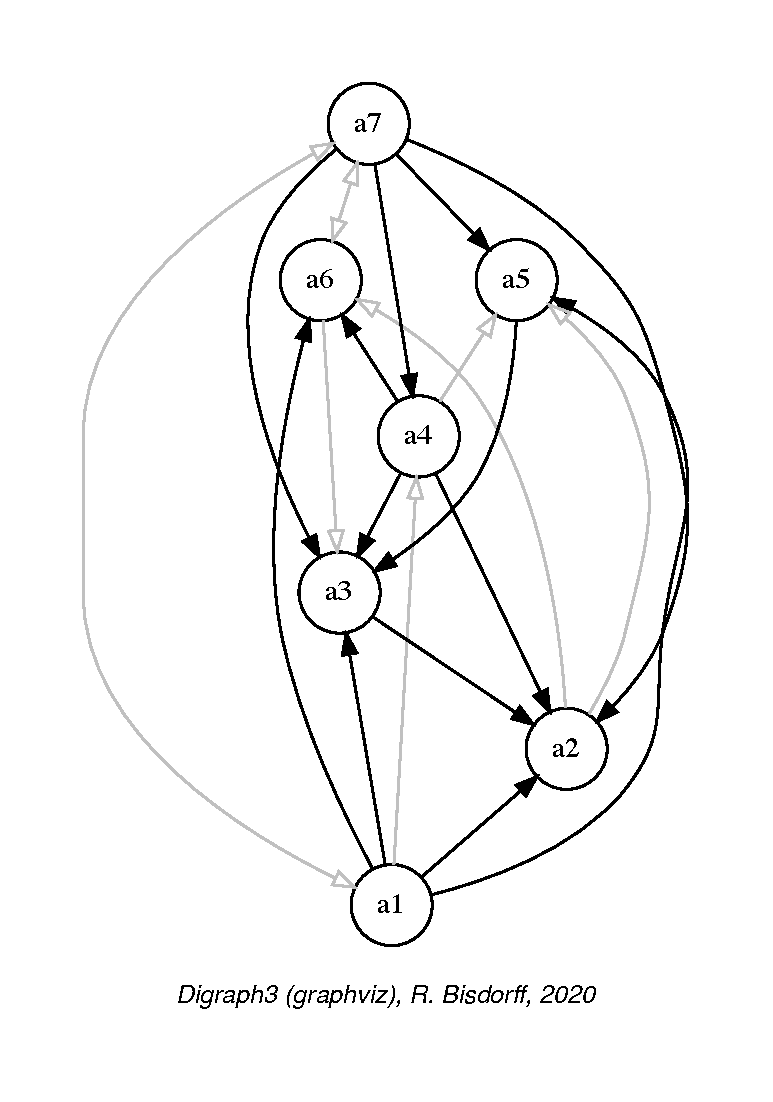
\includegraphics[width=5cm]{Figures/3-1-codualOdg.pdf}
\caption[The strict (codual) outranking digraph]{The strict (codual) outranking digraph. It becomes readily clear now from the picture that both alternatives \texttt{a1}  and \texttt{a7} are \emph{not outranked} by any other alternatives. Hence, \texttt{a1}  and \texttt{a7} appear as \emph{weak} \Condorcet winners and may be recommended as potential \emph{best} decision alternatives in this illustrative preference modelling example}
\label{fig:3.1}       % Give a unique label
\end{figure}
 
Many more tools for exploiting bipolar-valued outranking digraphs are available in the \Digraph resources \citep{BIS-2021b}.
\vspace{1cm}

In the methodological Part II, we present and discuss multiple criteria evaluation models and decision algorithms, like building a best choice recommendation, determining the winner of an election, computing linear rankings or quantile ratings with multiple incommensurable criteria.

%%%%%%%%%%%%%%%%%%%%%%%%%%%%%%%%%%%%
\phantomsection
\addcontentsline{toc}{section}{Notes}
\section*{Notes}

The seminal work on outranking digraphs goes back to the seventies and eighties when Bernard Roy \index{Roy@\textsl{B. Roy}} joined the just starting University Paris-Dauphine and founded there the '\emph{Laboratoire d’Analyse et de Modélisation de Systèmes pour l’Aide à la Décision}' (LAMSADE). The LAMSADE became the major site in the development of the outranking approach to multiple criteria decision aid. \citep*{ROY-1993}.

The ongoing success of the original \emph{outranking} concept stems from the fact that it is rooted in a sound pragmatism. The multiple criteria performance tableau, necessarily associated with a given outranking digraph, is indeed convincingly objective and meaningful \citep{ROY-1991}. And, ideas from social choice theory gave initially the insight that a pairwise voting mechanism à la \Condorcet could provide an order-statistical tool for aggregating a set of preference points of view into what M. Barbut\index{Barbut@\emph{M. Barbut}} called the \emph{central} \Condorcet point of view (\citealp{CON-1784} and \citealp{BAR-1980}); in fact the median of the multiple preference points of view, at minimal absolute \Kendall's\index{Kendall@\emph{M.G. Kendall}} ordinal correlation distance from all individual points of view (see Chap.~\ref{sec:16}).

Considering thus each performance criterion as a subset of unanimous voters and balancing the votes in favour against considerable counter-performances in disfavour gave eventually rise to the concept of \emph{outranking situation}, a distinctive feature of the Multiple Criteria Decision Aid approach \citep{BIS-2015}.  A modern definition would be : An alternative $x$ is said to \emph{outrank} alternative $y$ when – a \emph{significant majority} of criteria confirm that alternative $x$ has to be considered as \emph{at least as well evaluated as} an alternative $y$ (the \emph{concordance} argument); and – no discordant criterion opens to significant doubt the validity of the previous confirmation by revealing a considerable counter-performance of alternative $x$ compared to $y$ (the \emph{discordance} argument).

If the concordance argument was always well received, the discordance argument however, very confused in the beginning \citep{ROY-1966}, could only be handled in an epistemically correct and logically sound way by using a bipolar-valued epistemic logic (see Def.~\vref{def:3.1} and \citealp{BIS-2013}). The outranking situation had consequently to receive an explicit negative definition: An alternative $x$ is said to \emph{do not outrank} an alternative $y$ when – a \emph{significant majority} of criteria confirm that alternative $x$ has to be considered as \emph{not at least as well evaluated as} alternative $y$; and – no discordant criterion opens to significant doubt the validity of the previous confirmation by revealing a considerable \emph{better} performance of alternative $x$ compared to $y$.

Furthermore, the initial conjunctive aggregation of the concordance and discordance arguments had to be replaced by a disjunctive epistemic fusion operation, polarising in a logically and epistemically sound way the concordance with the discordance argument. This way, bipolar-valued outranking  digraphs gain two very useful properties from a measure theoretical perspective. They are \emph{weakly complete}; incomparability situations are no longer attested by the absence of positive outranking relations, but instead by epistemic indeterminateness. And they verify the \emph{coduality principle}: the negation of the epistemic ``\emph{at least as well evaluated as}'' situation corresponds formally to the strict converse epistemic ``\emph{less well evaluated than}'' situation.


%%%%%%% The chapter bibliography
%\normallatexbib
\clearpage
%\phantomsection
%\addcontentsline{toc}{section}{Chapter Bibliography}
%\chapter{Working with outranking digraphs}
\label{sec:3}

\abstract*{ In this chapter, we introduce the main formal object of this book, namely the bipolar-valued outranking digraph. With a randomly generated multiple criteria performance tableau, we construct the corresponding bipolar-valued outranking relation from pairwise comparisons. The resulting bipolar-valued outranking characteristics may be recoded. Finally, the codual outranking digraph gives us the associated strict outranking relation.}

\begin{quotation}
``\emph{The rule for the combination of independent concurrent arguments takes a very simple form when expressed in terms of the intensity of belief ... It is this: Take the sum of all the feelings of belief which would be produced separately by all the arguments pro, subtract from that the similar sum for arguments con, and the remainder is the feeling of belief which ought to have the whole. This is a proceeding which men often resort to, under the name of balancing reasons.}'' -- C.S. Peirce, The probability of induction (1878)
\end{quotation}
\vspace{1cm}

\abstract{ In this chapter, we introduce the main formal object of this book, namely the bipolar-valued outranking digraph. With a randomly generated multiple criteria performance tableau, we construct the corresponding bipolar-valued outranking relation from pairwise comparisons. The resulting bipolar-valued outranking characteristics may be recoded. Finally, the codual outranking digraph gives us the associated strict outranking relation.}


\section{The hybrid outranking digraph model}
\label{sec:3.1}

In the \texttt{outrankingDigraphs} module\index{outrankingDigraphs@\texttt{outrankingDigraphs} module}, the \texttt{BipolarOutrankingDigraph}\index{BipolarOutrankingDigraph@\texttt{BipolarOutrankingDigraph} class} class provides our standard \emph{outranking digraph} constructor. Such an instance represents a \emph{hybrid} object of both the \texttt{PerformanceTableau} type \emph{and} the \texttt{Outran\-kingDigraph} type \citep{BIS-2021b}.

A given \texttt{BipolarOutrankingDigraph} object contains hence always at least the following attributes:
\begin{enumerate}[topsep=3pt,partopsep=0pt]
\item \texttt{actions}: an ordered dictionary describing the potential decision actions or alternatives with \texttt{name} and \texttt{comment} attributes,
\item \texttt{objectives}: a possibly empty ordered dictionary of decision objectives with \texttt{name} and \texttt{comment} attributes, describing the multiple preference dimensions involved in the decision problem, 
\item \texttt{criteria}: an ordered dictionary of performance criteria, i.e. \emph{preferentially independent} and \emph{non-redundant} decimal-valued evaluation functions used for assessng the performance of each potential decision action with respect to a decision objective,
\item \texttt{evaluation}: a double dictionary gathering performance evaluations for each decision alternative on each criterion function. 
\item \texttt{valuationdomain}: a dictionary with three entries: the minimum ($-1.0$, \emph{certainly outranked}), the median ($0.0$, \emph{indeterminate}) and the maximum characteristic value ($+1.0$, \emph{certainly outranking}),
\item \texttt{relation}: a double dictionary defined on the Cartesian product of the set of decision alternatives capturing the credibility of the pairwise \emph{outranking situation} computed on the basis of the performance differences observed between couples of decision alternatives on the given family of criteria functions.   
\end{enumerate}

Let us consider, for instance, a random bipolar-valued outranking digraph with seven decision actions denoted \texttt{a1}, \texttt{a2}, ..., \texttt{a7}. We need therefore, first, to generate in Listing~\vref{list:3.1} a corresponding random performance tableau.
\begin{lstlisting}[caption={Generating a random performance tableau.},label=list:3.1]
>>> from perfTabs import RandomPerformanceTableau
>>> pt = RandomPerformanceTableau(numberOfActions=7,\
...                               seed=100)   
>>> pt
   *------- PerformanceTableau instance description ------*
    Instance class     : RandomPerformanceTableau
    Seed               : 100
    Instance name      : randomperftab
    Actions            : 7
    Criteria           : 7
    NaN proportion (%) : 6.1
>>> pt.showActions()
  *----- show digraphs actions --------------*
   key:  a1
    name:       action 1
    comment:    RandomPerformanceTableau() generated.
   key:  a2
    name:       action 2
    comment:    RandomPerformanceTableau() generated.
     ...
     ...
   key:  a7
    name:       action 7
    comment:    RandomPerformanceTableau() generated.
\end{lstlisting}

In this example we consider a family of seven \emph{equisignificant} cardinal \emph{criteria functions} \texttt{g1}, \texttt{g2}, ..., \texttt{g7}, measuring the performance of each alternative on a rational scale from $0.0$ (worst) to $100.00$ (best). In order to capture the evaluation procedures' potential \emph{uncertainty} and \emph{imprecision}, each criterion function \texttt{g1} to \texttt{g7} admits three performance \emph{discrimination thresholds} of $2.5$, $5.0$ and $80.0$ pts for warranting respectively any \emph{indifference}, \emph{preference} or \emph{considerable performance difference} situation.
\begin{lstlisting}[caption={Inspecting the performance criteria.},label=list:3.2]
>>> pt.showCriteria()
  *----  criteria -----*
   g1 'RandomPerformanceTableau() instance'
     Scale = [0.0, 100.0]
     Weight = 1.0
     Threshold ind : 2.50 + 0.00x ; percentile: 4.76
     Threshold pref : 5.00 + 0.00x ; percentile: 9.52
     Threshold veto : 80.00 + 0.00x ; percentile: 95.24
   g2 'RandomPerformanceTableau() instance'
     Scale = [0.0, 100.0]
     Weight = 1.0
     Threshold ind : 2.50 + 0.00x ; percentile: 6.67
     Threshold pref : 5.00 + 0.00x ; percentile: 6.67
     Threshold veto : 80.00 + 0.00x ; percentile: 100.00
      ...
      ...
   g7 'RandomPerformanceTableau() instance'
     Scale = [0.0, 100.0]
     Weight = 1.0
     Threshold ind : 2.50 + 0.00x ; percentile: 0.00
     Threshold pref : 5.00 + 0.00x ; percentile: 4.76
     Threshold veto : 80.00 + 0.00x ; percentile: 100.00
\end{lstlisting}

On criteria function \texttt{g1} (see Lines 6-8 in List.~\vref{list:3.2}) we observe, for instance, about $5\%$ of \emph{indifference} situations, about $90\%$ of \emph{preference} situations and about $5\%$ of \emph{considerable} performance difference situations.

The individual \emph{performance evaluation} of all decision alternative on each criterion are gathered in a \emph{performance table}.\index{showPerformanceTableau@\texttt{showPerformanceTableau()}}
\begin{lstlisting}[caption={Inspecting the performance evaluations},label=list:3.3]
>>> pt.showPerformanceTableau()
    *----  performance tableau -----*
     criteria |  'a1'  'a2'  'a3'  'a4'  'a5'  'a6'  'a7'   
     ---------|------------------------------------------
      'g1'    |  15.2  44.5  57.9  58.0  24.2  29.1  96.6  
      'g2'    |  82.3  43.9   NA   35.8  29.1  34.8  62.2  
      'g3'    |  44.2  19.1  27.7  41.5  22.4  21.5  56.9  
      'g4'    |  46.4  16.2  21.5  51.2  77.0  39.4  32.1  
      'g5'    |  47.7  14.8  79.7  67.5   NA   90.7  80.2  
      'g6'    |  69.6  45.5  22.0  33.8  31.8   NA   48.8  
      'g7'    |  82.9  41.7  12.8  21.9  75.7  15.4   6.0  
\end{lstlisting}

It is noteworthy to mention the three \emph{missing data} (\texttt{NA}) cases: action \texttt{a3} is missing, for instance, an evaluation on criterion \texttt{g2} (see Line 6 in List.~\vref{list:3.3}).
    
\section{The bipolar-valued outranking digraph}
\label{sec:3.2}

Given the previous random performance tableau \texttt{pt}, the \texttt{BipolarOutranking\-Digraph}\index{BipolarOutrankingDigraph@\texttt{BipolarOutrankingDigraph}} class constructor computes the corresponding \emph{bipolar-valued outranking digraph}. 
\begin{lstlisting}[caption={Example of random bipolar-valued outranking digraph.},label=list:3.4]
>>> from outrankingDigraphs import \
...                       BipolarOutrankingDigraph
>>> odg = BipolarOutrankingDigraph(pt)
>>> odg
  *------- Object instance description ------*
   Instance class       : BipolarOutrankingDigraph
   Instance name        : rel_randomperftab
   Actions              : 7
   Criteria             : 7
   Size                 : 20
   Determinateness (%)  : 63.27
   Valuation domain     : [-1.00;1.00]
   Attributes           : [
        'name', 'actions', 
	'criteria', 'evaluation', 'NA',
	'valuationdomain', 'relation', 
	'order', 'gamma', 'notGamma', ...
	]
\end{lstlisting}

The resulting digraph contains 20 positive (valid) outranking relations. And, the mean majority criteria significance support of all the pairwise outranking situations is $63.3\%$ (see Lines 9-10 in List.~\vref{list:3.4}).

We may inspect the complete $[-1.0,+1.0]$-valued adjacency table with the \texttt{showRelationTable()} method().\index{showRelationTable@\texttt{showRelationTable()}}
\begin{lstlisting}[caption={Inspecting the valued adjacency table.},label=list:3.5]
>>> odg.showRelationTable()
  * ---- Relation Table -----
   r(x,y)|  'a1'   'a2'   'a3'   'a4'   'a5'   'a6'   'a7'   
   ------|-------------------------------------------------
    'a1' | +1.00  +0.71  +0.29  +0.29  +0.29  +0.29  +0.00  
    'a2' | -0.71  +1.00  -0.29  -0.14  +0.14  +0.29  -0.57  
    'a3' | -0.29  +0.29  +1.00  -0.29  -0.14  +0.00  -0.29  
    'a4' | +0.00  +0.14  +0.57  +1.00  +0.29  +0.57  -0.43  
    'a5' | -0.29  +0.00  +0.14  +0.00  +1.00  +0.29  -0.29  
    'a6' | -0.29  +0.00  +0.14  -0.29  +0.14  +1.00  +0.00  
    'a7' | +0.00  +0.71  +0.57  +0.43  +0.29  +0.00  +1.00  
   Valuation domain: [-1.0; 1.0]
\end{lstlisting}

The \texttt{BipolarOutrankingDigraph}\index{BipolarOutrankingDigraph@\texttt{BipolarOutrankingDigraph}} class constructor computes from the given performance tableau $pt$ the characteristic value $r(x \succsim y)$ of a \emph{pairwise outranking} relation $x\, \succsim \,y$ in a default \emph{valuation domain} $[-1.0,+1.0]$ with the {\em median\/} value $0.0$ acting as \emph{indeterminate} characteristic value\footnote{See Definition~\vref{def:3.1} \citep{BIS-2013}}. 

\begin{definition}[Semantics of the bipolar-valued characteristic function $r$]\label{def:3.1}

\noindent The semantics of $r(x \succsim y)$ are the following:
\begin{itemize}[nosep]
\item [a.] When $r(x \succsim y) > 0.0$, it is more {\em True\/} than {\em False\/} that $x$ \emph{outranks} $y$, i.e. alternative $x$ is ``\emph{at least as well evaluated as}'' alternative $y$ on a weighted majority of criteria {\bf and} there is no considerable negative performance difference observed in disfavour of $x$,
\item [b.] When $r(x \succsim y) < 0.0$, it is more {\em False\/} than {\em True\/} that $x$ \emph{outranks} $y$, i.e. alternative $x$ is {\bf not} ``\emph{at least as well evaluated as} alternative $y$ on a weighted majority of criteria than alternative $y$ {\bf and} there is no considerable positive performance difference observed in favour of $x$,
\item [c.] When $r(x \succsim y) = 0.0$, it is {\bf indeterminate} whether $x$ outranks $y$ or not.
\end{itemize}
\end{definition}

\section{Pairwise comparisons}
\label{sec:3.3}

From above given semantics, we notice in line 5 in Listing~\vref{list:3.5} that \texttt{a1} outranks \texttt{a2}: $r(a1 \succsim a2) + 0.71$), but not \texttt{a7}: $r(a1 \succsim a7) = 0.0$). In order to comprehend the characteristic values shown in the outranking relation table, we can inspect with the \texttt{showPairwiseComparison()} method\index{showPairwiseComparison@\texttt{showPairwiseComparison()}} the details of the pairwise multiple criteria comparison between, for instance, alternatives \texttt{a1} and \texttt{a2}.
\begin{lstlisting}[caption={Inspecting a pairwise multiple criteria comparison},label=list:3.6]
>>> odg.showPairwiseComparison('a1','a2')
  *------------  pairwise comparison ----*
   Comparing actions : (a1, a2)
   crit. wght. g(a1)  g(a2)   diff  | ind   pref    r() 
   -------------------------------  	 --------------------
    g1   1.00  15.17  44.51  -29.34 | 2.50  5.00   -1.00 
    g2   1.00  82.29  43.90  +38.39 | 2.50  5.00   +1.00 
    g3   1.00  44.23  19.10  +25.13 | 2.50  5.00   +1.00 
    g4   1.00  46.37  16.22  +30.15 | 2.50  5.00   +1.00 
    g5   1.00  47.67  14.81  +32.86 | 2.50  5.00   +1.00 
    g6   1.00  69.62  45.49  +24.13 | 2.50  5.00   +1.00 
    g7   1.00  82.88  41.66  +41.22 | 2.50  5.00   +1.00 
    Valuation in range: -7.00 to +7.00;          -------
       r(a1,a2): +5.00/7.00 = +0.71                +5.00
\end{lstlisting}

The outranking characteristic value $r(a1 \succsim a2)$ represents the relative \emph{majority margin} resulting from the difference between the significance weights of the criteria in favour and the significance weights of the criteria in disfavour of the statement that alternative \texttt{a1} is ``\emph{at least as well evaluated as}'' alternative \texttt{a2}. No considerable performance difference being observed, no polarising situation is triggered in this pairwise comparison.

Such a polarised situation is however observed when we compare the evaluations of alternatives \texttt{a1} and \texttt{a7} with the \texttt{showPairwiseOutrankings()} method. \index{showPairwiseoutrankings@\texttt{showPairwiseOutrankings()}}
\begin{lstlisting}[caption={Pairwise comparison with considerable performance difference},label=list:3.7,basicstyle=\ttfamily\scriptsize]
>>> odg.showPairwiseoutrankings('a1','a7')
  *------------  pairwise comparison ----*
   Comparing actions : (a1, a7)
   crit. wght. g(a1)  g(a7)   diff  | ind   pref    r()  |  v     veto
   -------------------------------   ------------------   -----------
    g1   1.00  15.17  96.58  -81.41 | 2.50  5.00   -1.00 | 80.00 -1.00
    g2   1.00  82.29  62.22  +20.07 | 2.50  5.00   +1.00 | 
    g3   1.00  44.23  56.90  -12.67 | 2.50  5.00   -1.00 | 
    g4   1.00  46.37  32.06  +14.31 | 2.50  5.00   +1.00 | 
    g5   1.00  47.67  80.16  -32.49 | 2.50  5.00   -1.00 | 
    g6   1.00  69.62  48.80  +20.82 | 2.50  5.00   +1.00 | 
    g7   1.00  82.88   6.05  +76.83 | 2.50  5.00   +1.00 | 
   ----------------------------------------
   Valuation in range: -7.00 to +7.00; r(x,y)= +1/7 => 0.0
  *------------  pairwise comparison ----*
   Comparing actions : (a1, a7)
   crit. wght. g(a7)  g(a1)   diff  | ind   pref    r()  |  v     veto
   -------------------------------   ------------------   -----------
    g1   1.00  96.58  15.17  +81.41 | 2.50  5.00   +1.00 | 80.00 +1.00
    g2   1.00  62.22  82.29  -20.07 | 2.50  5.00   -1.00 | 
    g3   1.00  56.90  44.23  +12.67 | 2.50  5.00   +1.00 | 
    g4   1.00  32.06  46.37  -14.31 | 2.50  5.00   -1.00 | 
    g5   1.00  80.16  47.67  +32.49 | 2.50  5.00   +1.00 | 
    g6   1.00  48.80  69.62  -20.82 | 2.50  5.00   -1.00 | 
    g7   1.00   6.05  82.88  -76.83 | 2.50  5.00   -1.00 | 
   ----------------------------------------
   Valuation in range: -7.00 to +7.00; r(x,y)= -1/7 => 0.0
\end{lstlisting}

This time, we observe a $(1/7 + 1)/2 = 57.1\%$ majority of criteria significance warranting a ``\emph{at least as well evaluated as}'' situation between alternative \texttt{a1} and alternative \texttt{a7}. Yet, we also observe a considerable \emph{negative} performance difference on criterion \texttt{g1} (see Line 6 in List.~\vref{list:3.7}). Both contradictory facts trigger eventually in Line 14 an \emph{indeterminate} outranking situation. The inverse polarisation effect appears when considering in Lines 19-25 the converse performance differences between alternative \texttt{a7} and alternative \texttt{a1}. The considerable better performing situation on criterion \texttt{g1} makes doubtful the otherwise ``\emph{not at least as well evaluated as}'' situation (see Lines 19 and 27).

Notice that the occurrence in a pairwise comparison of conjointly considerable positive and negative performance differences will also trigger an indeterminate outranking situation. When observing at the same time a positive (resp. negative) ``\emph{at least as well evaluated as}'' situation and one or more considerable positive (resp. negative) performance difference, the outranking situation gets validated (resp. invalidated) for certain \citep{BIS-2013}.

\section{Recoding the characteristic valuation domain}
\label{sec:3.4}

All outranking digraphs, being of root \texttt{Digraph} type, inherit the methods available under this latter class. The characteristic valuation domain of a digraph can, for instance, be recoded with the \texttt{recodeValuation()}\index{recodeValuation@\emph{recodeValuation()}} method to the \emph{integer} range $[-7,+7]$, i.e. plus or minus the total significance weights of the family of criteria considered in this example instance \texttt{odg}.
\begin{lstlisting}[caption={Recoding the digraph valuation},label=list:3.8]
>>> odg.recodeValuation(-7,+7)
>>> odg.valuationdomain['hasIntegerValuation'] = True
>>> Digraph.showRelationTable(odg,ReflexiveTerms=False)
  * ---- Relation Table -----
   r(x,y)  |  'a1'  'a2'  'a3'  'a4'  'a5'  'a6'  'a7'	  
  ---------|------------------------------------------
    'a1'   |    -    +5    +2    +2    +2    +2     0	 
    'a2'   |   -5     -    -1    -1    +1    +2    -4	 
    'a3'   |   -1    +2     -    -1    -1     0    -1	 
    'a4'   |    0    +1    +4     -    +2    +4    -3	 
    'a5'   |   -1     0    +1     0     -    +2    -1	 
    'a6'   |   -1     0    +1    -1    +1     -     0	 
    'a7'   |    0    +5    +4    +3    +2     0     -	 
    Valuation domain: [-7;+7]
\end{lstlisting}

Notice in Listing~\vref{list:3.8} that the self comparison characteristics $r(x \succsim x)$ may be ignored by setting the \texttt{ReflexiveTerms} Boolean parameter to \texttt{False}. Mind that the trivial reflexive terms of outranking relations are ignored in some of the \Digraph methods. 

\section{The strict outranking digraph}
\label{sec:3.5}

From theory we know that a bipolar-valued outranking digraph is \emph{weakly complete}, i.e. if $r(x \succsim y) < 0.0$ then $r(y \succsim x) \geq 0.0$. From this property follows that a bipolar-valued outranking digraph verifies the \emph{coduality principle}\index{coduality principle}: the \emph{dual}\footnote{Not to be confused with the dual graph of a plane graph $g$ that has a vertex for each face of $g$. Here we mean the \emph{less than} (strict converse) relation corresponding to a \emph{greater or equal} relation, or the \emph{less than or equal} relation corresponding to a (strict) \emph{better than} relation.} --strict negation-- of the \emph{converse} --inverse-- of the outranking relation $(x \succsim y)$ corresponds to its asymmetric \emph{strict outranking} part $(x \succnsim y)$  \citep{BIS-2013, ADT-L7}.

We may visualize the \emph{codual} (\emph{strict}) outranking digraph with a graphviz drawing \footnote{The \texttt{exportGraphViz()} method is depending on drawing tools from the graphviz software (https://graphviz.org/). On Linux Ubuntu or Debian you may try \texttt{sudo apt-get install graphviz} to install them. There are ready \emph{dmg} installers for Mac OSX.}.\index{graphviz}
\begin{lstlisting}
>>> cdodg = -(~odg)
>>> cdodg.exportGraphViz('codualOdg')
  *---- exporting a dot file for GraphViz tools ---------*
   Exporting to codualOdg.dot
   dot -Grankdir=BT -Tpng codualOdg.dot -o codualOdg.png
\end{lstlisting}
\begin{figure}[ht]
\sidecaption[t]
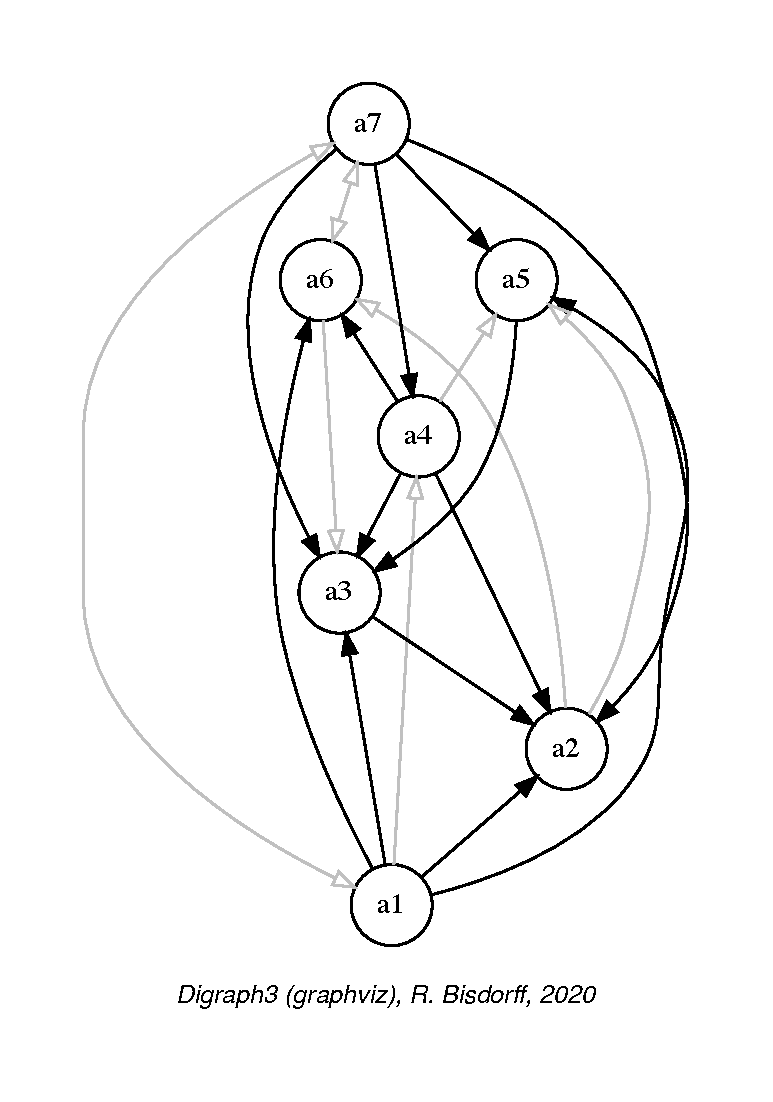
\includegraphics[width=5cm]{Figures/3-1-codualOdg.pdf}
\caption[The strict (codual) outranking digraph]{The strict (codual) outranking digraph. It becomes readily clear now from the picture that both alternatives \texttt{a1}  and \texttt{a7} are \emph{not outranked} by any other alternatives. Hence, \texttt{a1}  and \texttt{a7} appear as \emph{weak} \Condorcet winners and may be recommended as potential \emph{best} decision alternatives in this illustrative preference modelling example}
\label{fig:3.1}       % Give a unique label
\end{figure}
 
Many more tools for exploiting bipolar-valued outranking digraphs are available in the \Digraph resources \citep{BIS-2021b}.
\vspace{1cm}

In the methodological Part II, we present and discuss multiple criteria evaluation models and decision algorithms, like building a best choice recommendation, determining the winner of an election, computing linear rankings or quantile ratings with multiple incommensurable criteria.

%%%%%%%%%%%%%%%%%%%%%%%%%%%%%%%%%%%%
\phantomsection
\addcontentsline{toc}{section}{Notes}
\section*{Notes}

The seminal work on outranking digraphs goes back to the seventies and eighties when Bernard Roy \index{Roy@\textsl{B. Roy}} joined the just starting University Paris-Dauphine and founded there the '\emph{Laboratoire d’Analyse et de Modélisation de Systèmes pour l’Aide à la Décision}' (LAMSADE). The LAMSADE became the major site in the development of the outranking approach to multiple criteria decision aid. \citep*{ROY-1993}.

The ongoing success of the original \emph{outranking} concept stems from the fact that it is rooted in a sound pragmatism. The multiple criteria performance tableau, necessarily associated with a given outranking digraph, is indeed convincingly objective and meaningful \citep{ROY-1991}. And, ideas from social choice theory gave initially the insight that a pairwise voting mechanism à la \Condorcet could provide an order-statistical tool for aggregating a set of preference points of view into what M. Barbut\index{Barbut@\emph{M. Barbut}} called the \emph{central} \Condorcet point of view (\citealp{CON-1784} and \citealp{BAR-1980}); in fact the median of the multiple preference points of view, at minimal absolute \Kendall's\index{Kendall@\emph{M.G. Kendall}} ordinal correlation distance from all individual points of view (see Chap.~\ref{sec:16}).

Considering thus each performance criterion as a subset of unanimous voters and balancing the votes in favour against considerable counter-performances in disfavour gave eventually rise to the concept of \emph{outranking situation}, a distinctive feature of the Multiple Criteria Decision Aid approach \citep{BIS-2015}.  A modern definition would be : An alternative $x$ is said to \emph{outrank} alternative $y$ when – a \emph{significant majority} of criteria confirm that alternative $x$ has to be considered as \emph{at least as well evaluated as} an alternative $y$ (the \emph{concordance} argument); and – no discordant criterion opens to significant doubt the validity of the previous confirmation by revealing a considerable counter-performance of alternative $x$ compared to $y$ (the \emph{discordance} argument).

If the concordance argument was always well received, the discordance argument however, very confused in the beginning \citep{ROY-1966}, could only be handled in an epistemically correct and logically sound way by using a bipolar-valued epistemic logic (see Def.~\vref{def:3.1} and \citealp{BIS-2013}). The outranking situation had consequently to receive an explicit negative definition: An alternative $x$ is said to \emph{do not outrank} an alternative $y$ when – a \emph{significant majority} of criteria confirm that alternative $x$ has to be considered as \emph{not at least as well evaluated as} alternative $y$; and – no discordant criterion opens to significant doubt the validity of the previous confirmation by revealing a considerable \emph{better} performance of alternative $x$ compared to $y$.

Furthermore, the initial conjunctive aggregation of the concordance and discordance arguments had to be replaced by a disjunctive epistemic fusion operation, polarising in a logically and epistemically sound way the concordance with the discordance argument. This way, bipolar-valued outranking  digraphs gain two very useful properties from a measure theoretical perspective. They are \emph{weakly complete}; incomparability situations are no longer attested by the absence of positive outranking relations, but instead by epistemic indeterminateness. And they verify the \emph{coduality principle}: the negation of the epistemic ``\emph{at least as well evaluated as}'' situation corresponds formally to the strict converse epistemic ``\emph{less well evaluated than}'' situation.


%%%%%%% The chapter bibliography
%\normallatexbib
\clearpage
%\phantomsection
%\addcontentsline{toc}{section}{Chapter Bibliography}
%\input{02-mainMatters/03-chapterOutrankingDigraphs.bbl}
\bibliographystyle{spbasic}
\bibliography{03-backMatters/reference}

\bibliographystyle{spbasic}
\bibliography{03-backMatters/reference}

\bibliographystyle{spbasic}
\bibliography{03-backMatters/reference}


%%%%%%%%%%%%%%%%%%%%%part.tex%%%%%%%%%%%%%%%%%%%%%%%%%%%%%%%%%%
% 
% sample part title
%
% Use this file as a template for your own input.
%
%%%%%%%%%%%%%%%%%%%%%%%% Springer %%%%%%%%%%%%%%%%%%%%%%%%%%

\begin{partbacktext}
  \part{Evaluation models and decision methods and tools}

  \begin{quotation}''... whether we are deciding between buying different commodity baskets, or making choices about what to do on a holiday, or deciding for whom to vote for in an election, we are inescapably involved in evaluating alternatives with non–commensurable aspects.''
    
    --Amartya Sen\index{Sen@\textsl{A. Sen}} \emph{Idea of Justice}, Allen Lane London, 2009.
  \end{quotation}

  \vspace{1cm}
  \noindent The second and main Part of the book presents in eight chapters decision methods and computational tools for selecting a best decision alternative, for ranking the potential decision alternative from best to worst, for relative and absolute rating with the help of bipolar-valued outranking digraphs. We also show how to edit a new multiple criteria performance tableau and present several models of random performance tableau generators. A last chapter is devoted to HPC ranking of big performance tableaux.
\end{partbacktext}
\chapter{How to create a new performance tableau instance}
\label{sec:4}

\abstract*{To be written.}

\abstract{To be written.}

In this tutorial we illustrate a way of creating a new {\em PerformanceTableau\/} instance by editing a template with 5 decision alternatives, 3 decision objectives and 6 performance criteria. 

\section{Editing a template file}
\label{sec:4.1}

For this purpose we provide the following {\tt perfTab\_Template.py} file in the \texttt{examples} directory of the \Digraph resources.

\begin{lstlisting}[caption={PerformanceTableau object template},label=list:4.1,basicstyle=\footnotesize]
   ###############################################
   # Digraph3 documentation
   # Template for creating a new PerformanceTableau instance
   # (C) R. Bisdorff Mar 2021
   # Digraph3/examples/perfTab_Template.py
   ###############################################
   from decimal import Decimal
   from collections import OrderedDict
   #####
   # edit the decision actions
   # avoid special characters, like '_', '/' or ':',
   # in action identifiers and short names
   actions = OrderedDict([
    ('a1', {
     'shortName': 'action1',
     'name': 'decision alternative a1',
     'comment': 'some specific features of this alternative',
      }),
     ...
     ...
   ])
   #####
   # edit the decision objectives
   # adjust the list of performance criteria
   # and the total weight (sum of the criteria weights)
   # per objective
   objectives = OrderedDict([
    ('obj1', {
     'name': 'decision objective obj1',
     'comment': "some specific features of this objective",
     'criteria': ['g1', 'g2'],
     'weight': Decimal('6'),
     }),
     ...
     ...
    ])
   #####
   # edit the performance criteria
   # adjust the objective reference
   # Left Decimal of a threshold = constant part and
   #  right Decimal = proportional part of the threshold 
   criteria = OrderedDict([
    ('g1', {
     'shortName': 'crit1',
     'name': "performance criteria 1",
     'objective': 'obj1',
     'preferenceDirection': 'max',
     'comment': 'measurement scale type and unit',
     'scale': (Decimal('0.0'), Decimal('100.0'),
     'thresholds': {'ind':  (Decimal('2.50'), Decimal('0.0')),
		    'pref': (Decimal('5.00'), Decimal('0.0')),
		    'veto': (Decimal('60.00'), Decimal('0.0'))
                   },
     'weight': Decimal('3'),
     }),
     ...
     ...
    ])
   #####
   # default missing data symbol = -999
   NA = Decimal('-999')
   #####
   # edit the performance evaluations
   # criteria to be minimized take negative grades
   evaluation = {
    'g1': {
       'a1':Decimal("41.0"),
       'a2':Decimal("100.0"),
       'a3':Decimal("63.0"),
       'a4':Decimal('23.0'),
       'a5': NA,
      },
    # g2 is of ordinal type and scale 0-10
    'g2': {
       'a1':Decimal("4"),
       'a2':Decimal("10"),
       'a3':Decimal("6"),
       'a4':Decimal('2'),
       'a5':Decimal('9'),
      },
    # g3 has preferenceDirection = 'min'
    'g3': {
       'a1':Decimal("-52.2"),
       'a2':NA,
       'a3':Decimal("-47.3"),
       'a4':Decimal('-35.7'),
       'a5':Decimal('-68.00'),
      },
    ...
    ...
    }
   ####################
\end{lstlisting}

The template file, shown in Listing \ref{list:4.1}, contains first the instructions to import the required {\tt Decimal} and {\tt OrderedDict} classes (see Lines 7-8). Four main sections are following: the potential decision {\bf actions}, the decision \textbf{objectives}, the performance \textbf{criteria}, and finally the performance \textbf{evaluation}.  

\section{Editing the decision alternatives}
\label{sec:4.2}

Decision alternatives are stored in attribute \textbf{actions} under the \texttt{OrderedDict} format (see the \href{https://docs.python.org/3/library/collections.html}{{\tt OrderedDict}} description in the Python documentation).

Required attributes of each decision alternative, besides the object identifier,  are: \texttt{shortName}, \texttt{name} and \texttt{}comment (see Lines 15-17). The \texttt{shortName} attribute is essentially used when showing the performance tableau or the performance heatmap in a browser view.

\begin{svgraybox}Mind that graphviz drawings require digraph actions' (nodes) identifier strings without any special characters like `\_` or `/`.\end{svgraybox}

Decision actions descriptions are stored in the order of which they appear in the stored instance file. The \texttt{OrderedDict} object keeps this given order when iterating over the decision alternatives.

The random performance tableau models presented in the previous tutorial use the \texttt{actions} attribute for storing special features of the decision alternatives. The \emph{Cost-Benefit} model, for instance, uses a \texttt{type} attribute for distinguishing between \emph{advantageous}, \emph{neutral} and \emph{cheap} alternatives. The \emph{3-Objectives} model keeps a detailed record of the performance profile per decision objective and the corresponding random generators per performance criteria (see Lines 7- below).

\begin{lstlisting}[basicstyle=\footnotesize]
>>> t = Random3ObjectivesPerformanceTableau()
>>> t.actions
    OrderedDict([
     ('p01', {'shortName': 'p01',
              'name': 'action p01 Eco~ Soc- Env+',
              'comment': 'random public policy',
	      'Eco': 'fair',
	      'Soc': 'weak',
	      'Env': 'good',
              'profile': {'Eco':'fair',
	                  'Soc':'weak',
			  'Env':'good'}
              'generators': {'ec01': ('triangular', 50.0, 0.5),
                             'so02': ('triangular', 30.0, 0.5),
		             'en03': ('triangular', 70.0, 0.5),
		             ...
		             },
              }
         ),
      ...
      ])
\end{lstlisting}

The second section of the template file concerns the decision \textbf{objectives}.

\section{Editing the decision objectives}
\label{sec:4.3}

The minimal required attributes (see Listing \ref{list:4.1} Lines 27-33) of the ordered decision \textbf{objectives} dictionary, besides the individual objective identifiers, are \texttt{name}, \texttt{comment}, \texttt{criteria} (the list of significant performance criteria) and \texttt{weight} (the importance of the decision objective). The latter attribute contains the sum of the \emph{significance} weights of the objective's criteria list. 

The \texttt{objectives} attribute is methodologically useful for specifying the performance criteria significance in building decision recommendations. Mostly, we assume indeed that decision objectives are all equally important and the performance criteria are equi-significant per objective. This is, for instance, the default setting in the random \emph{3-Objectives} performance tableau model.

\begin{lstlisting}[caption={Example of decision objectives' description},label=list:4.2,basicstyle=\footnotesize]
>>> t = Random3ObjectivesPerformanceTableau()
>>> t.objectives
 OrderedDict([
 ('Eco',
  {'name': 'Economical aspect',
   'comment': 'Random3ObjectivesPerformanceTableau generated',
   'criteria': ['ec01', 'ec06', 'ec09'],
   'weight': Decimal('48')}),
  ('Soc',
   {'name': 'Societal aspect',
    'comment': 'Random3ObjectivesPerformanceTableau generated',
    'criteria': ['so02', 'so12'],
    'weight': Decimal('48')}),
  ('Env',
   {'name': 'Environmental aspect',
    'comment': 'Random3ObjectivesPerformanceTableau generated',
    'criteria': ['en03', 'en04', 'en05', 'en07',
                 'en08', 'en10', 'en11', 'en13'],
    'weight': Decimal('48')})
 ])
\end{lstlisting}

The importance weight sums up to 48 for each one of the three example decision objectives shown in Listing \ref{list:4.2} (Lines 8,13 and 19), so that the significance of each one of the 3 economic criteria is set to 16, of both societal criteria is set to 24, and of each one of the 6 environmental criteria is set to 8.

\begin{svgraybox}Mind that the \texttt{objectives} attribute is always present in a \texttt{PerformanceTableau} object instance, even when empty. In this case, we consider that each performance criterion canonically represents in fact its own decision objective. The criterion significance equals in this case the corresponding decision objective's importance weight.\end{svgraybox}

The third section of the template file concerns now the \textbf{performance criteria}.

\section{Editing the family of performance criteria}
\label{sec:4.4}

In order to assess how well each potential decision alternative is satisfying a given decision objective, we need \emph{performance criteria}, i.e. decimal-valued grading functions gathered in an ordered \texttt{criteria} dictionary. The required attributes (see Listing \ref{list:4.3}), besides the criteria identifiers, are the usual \texttt{shortName}, \texttt{name} and \texttt{comment}. Specific for a criterion are furthermore the \texttt{objective} reference, the significance \texttt{weight}, the grading \texttt{scale} (minimum and  maximum performance values), the \texttt{preferenceDirection} ('max' or 'min') and the performance discrimination \texttt{thresholds} attributes.

\begin{lstlisting}[caption={Example of performance criteria description},label=list:4.3,basicstyle=\footnotesize]
   criteria = OrderedDict([
    ('g1', {
     'shortName': 'crit1',
     'name': "performance criteria 1",
     'comment': 'measurement scale type and unit',
     'objective': 'obj1',
     'weight': Decimal('3'),
     'scale': (Decimal('0.0'), Decimal('100.0'),
     'preferenceDirection': 'max',
     'thresholds': {'ind':  (Decimal('2.50'), Decimal('0.0')),
		    'pref': (Decimal('5.00'), Decimal('0.0')),
		    'veto': (Decimal('60.00'), Decimal('0.0'))
                   },
     }),
    ...
    ...])
\end{lstlisting}

In our bipolar-valued outranking approach, all performance criteria implement \emph{decimal-valued} grading functions, where preferences are either \emph{increasing} or \emph{decreasing} with measured performances.

\begin{svgraybox}In order to model a \textbf{coherent} performance tableau, the decision criteria must satisfy two methodological requirements:
\begin{enumerate}
\item \textbf{Independance}: Each decision criterion implements a grading that is \emph{functionally independent} of the grading of the other decision criteria, i.e. the performance measured on one of the criteria does not \emph{constrain} the performance measured on any other criterion.
\item \textbf{Non redundancy}: Each performance criterion is only \emph{significant} for a \emph{single} decision objective.
\end{enumerate}
\end{svgraybox}

In order to take into account any, usually \emph{unavoidable}, \textbf{imprecision} of the performance grading procedures, we may specify three performance \textbf{discrimination thresholds}: an \emph{indifference} ('ind'), a \emph{preference} ('pref') and a \emph{considerable performance difference} ('veto') threshold (see Listing \ref{list:4.3} Lines 10-12). The left decimal number of a threshold description tuple indicates a \emph{constant part}, whereas the right decimal number indicates a \emph{proportional} part.

On the template performance criterion $g_1$, shown in Listing \ref{list:4.3}, we observe for instance a grading scale from $0.0$ to $100.0$ with a constant \emph{indifference} threshold of $2.5$, a constant \emph{preference} threshold of $5.0$, and a constant \emph{considerable performance difference} threshold of $60.0$. The latter threshold  will trigger, the case given, a \emph{polarisation} of the outranking statement [BIS-2013].

In a random \emph{Cost-Benefit} performance tableau model we may obtain by default the following content.

\begin{lstlisting}[caption={Example of cardinal Costs criterion},label=list:4.4,basicstyle=\footnotesize]
>>> tcb = RandomCBPerformanceTableau()
>>> tcb.showObjectives()
 *------ decision objectives -------*
 C: Costs
   c1 random cardinal cost criterion 6
   Total weight: 6.00 (1 criteria)
   ...
   ...
>>> tcb.criteria
 OrderedDict([
  ('c1', {'preferenceDirection': 'min',
          'scaleType': 'cardinal',
	  'objective': 'C',
	  'shortName': 'c1',
	  'name': 'random cardinal cost criterion',
	  'scale': (0.0, 100.0),
	  'weight': Decimal('6'),
	  'randomMode': ['triangular', 50.0, 0.5],
	  'comment': 'Evaluation generator: triangular law ...',
          'thresholds': OrderedDict([
	     ('ind', (Decimal('1.49'), Decimal('0'))),
	     ('pref', (Decimal('3.7'), Decimal('0'))),
	     ('veto', (Decimal('67.71'), Decimal('0')))
             ])
           }),
  ...
  ...
 ])
\end{lstlisting}

Criterion $c1$ appears here (see Listing \ref{list:4.4}) to be a cardinal criterion to be minimized and significant for the \emph{Costs} ($C$) decision objective. We may use the {\tt showCriteria()} method for printing the corresponding performance discrimination thresholds.

\begin{lstlisting}[basicstyle=\footnotesize]
>>> tcb.showCriteria(IntegerWeights=True)
 *----  criteria -----*
  c1 'Costs/random cardinal cost criterion'
    Scale = (0.0, 100.0)
    Weight = 6 
    Threshold ind : 1.49 + 0.00x ; percentile: 5.13
    Threshold pref : 3.70 + 0.00x ; percentile: 10.26
    Threshold veto : 67.71 + 0.00x ; percentile: 96.15
\end{lstlisting}

The \emph{indifference} threshold on this criterion amounts to a constant value of $1.49$ (Line 6 above). More or less $5\%$ of the observed performance differences on this criterion appear hence to be \textbf{insignificant}. Similarly, with a preference threshold of $3.70$, about $90\%$ of the observed performance differences are preferentially \textbf{significant} (Line 7). Furthermore, $100.0 - 96.15 = 3.85\%$ of the observed performance differences appear to be \textbf{considerable} (Line 8) and will trigger a \emph{polarisation} of the corresponding outranking statements.

After the performance criteria description, we are ready for recording the actual \textbf{performance table}.

\section{Editing the performance table}
\label{sec:4.5}

The individual grades of each decision alternative on each decision criterion are recorded in a double \emph{criterion} x \emph{action} dictionary called \texttt{evaluation} (see Listing \ref{list:4.4}). As we may encounter missing data cases, we previously define a \emph{missing data} symbol \texttt{NA} which is set here to a value disjoint from all the measurement scales, by default \texttt{Decimal('-999')} (Line 2).

\begin{lstlisting}[caption={Editing performance grades},label=list:4.5,basicstyle=\footnotesize]
#----------
NA = Decimal('-999')
#----------
evaluation = {
  'g1': {
     'a1':Decimal("41.0"),
     'a2':Decimal("100.0"),
     'a3':Decimal("63.0"),
     'a4':Decimal('23.0'),
     'a5': NA,  # missing data
   },
   ...
   ...
  # g3 has preferenceDirection = 'min'
  'g3': {
     'a1':Decimal("-52.2"), # negative grades
     'a2':NA,
     'a3':Decimal("-47.3"),
     'a4':Decimal('-35.7'),
     'a5':Decimal('-68.00'),
   },
   ...
   ...
}
\end{lstlisting}

Notice in Listing \ref{list:4.4} (Lines 16- ) that on a criterion with \texttt{preferenceDirection} = 'min' all performance grades are recorded as \textbf{negative} values.

We may now inspect the eventually recorded complete template performance table.

\begin{lstlisting}[basicstyle=\footnotesize]
>>> from perfTabs import PerformanceTableau   
>>> t = PerformanceTableau('perfTab_Template')
>>> t.showPerformanceTableau(ndigits=1)
 *----  performance tableau -----*
  Criteria  |  'g1'   'g2'  'g3'  'g4'   'g5'   'g6'   
  Actions   |    3      3     6     2      2      2    
   ---------|-----------------------------------------
  'action1' |  41.0   4.0  -52.2  71.0   63.0   22.5  
  'action2' | 100.0  10.0    NA   89.0   30.7   75.0  
  'action3' |  63.0   6.0  -47.3  55.4   63.5    NA   
  'action4' |  23.0   2.0  -35.7  83.5   37.5   54.9  
  'action5' |   NA    9.0  -68.0  10.0   88.0   75.0
\end{lstlisting}

We may furthermore compute the associated outranking digraph and check if we observe any polarised outranking situtations.

\begin{lstlisting}[basicstyle=\footnotesize]
>>> from outrankingDigraphs import BipolarOutrankingDigraph
>>> g = BipolarOutrankingDigraph(t)
>>> g.showVetos()
 *----  Veto situations ---
  number of veto situations : 1 
  1: r(a4 >= a2) = -0.44
     criterion: g1
     Considerable performance difference : -77.00
     Veto discrimination threshold       : -60.00
     Polarisation: r(a4 >= a2) = -0.44 ==> -1.00
 *----  Counter-veto situations ---
  number of counter-veto situations : 1 
  1: r(a2 >= a4) = 0.56
     criterion: g1
     Considerable performance difference : 77.00
     Counter-veto threshold              : 60.00
     Polarisation: r(a2 >= a4) = 0.56 ==> +1.00
\end{lstlisting}

Indeed, due to the considerable performance difference ($77.00$) oberved on performance criterion $g1$, alternative $a2$ \textbf{for sure} \emph{outranks} alternative $a4$, respectively $a4$ \textbf{for sure} \emph{does not outrank} $a2$.

\section{Inspecting the template outranking relation}
\label{sec:4.6}

Let us have a look at the outranking relation table.

\begin{lstlisting}[caption={The template outranking relation},label=list:4.5,basicstyle=\footnotesize]
>>> g.showRelationTable()
 * ---- Relation Table -----
   r   |  'a1'   'a2'   'a3'   'a4'   'a5'   
  -----|-----------------------------------
  'a1' | +1.00  -0.44  -0.22  -0.11  +0.06  
  'a2' | +0.44  +1.00  +0.33  +1.00  +0.28  
  'a3' | +0.67  -0.33  +1.00  +0.00  +0.17  
  'a4' | +0.11  -1.00  +0.00  +1.00  +0.06  
   'a5' | -0.06  -0.06  -0.17  -0.06  +1.00
\end{lstlisting}

We may notice in the outranking relation table above (see Listing \ref{list:4.5}) that decision alternative $a2$ positively \textbf{outranks} all the other four alternatives  (Line 6). Similarly, alternative $a5$ is positively \textbf{outranked} by all the other alternatives (see Line 9). We may orient this way the \emph{graphviz} drawing of the template outranking digraph. 

\begin{lstlisting}[basicstyle=\footnotesize]
>>> g.exportGraphViz(fileName= 'template',\
...                  bestChoice =['a2'],\
...                  worstChoice=['a5'])
  *---- exporting a dot file for GraphViz tools ---------*
   Exporting to template.dot
   dot -Grankdir=BT -Tpng template.dot -o template.png
\end{lstlisting}
    
\begin{figure}[h]
\sidecaption
\includegraphics[width=4cm]{Figures/template.png}
\caption{The template outranking digraph models in fact a \textbf{partial order} on the five potential decision alternatives. Alternatives \emph{action3} ($a3$ ) and \emph{action4} ($a4$) appear actually \textbf{incomparable}.}
\label{fig:4.1}       % Give a unique label
\end{figure}

In Listing \ref{list:4.5} their pairwise outranking characteritics show indeed the \textbf{indeterminate} value $0.00$ (Lines 7-8). We may check their pairwise comparison as follows.

\begin{lstlisting}[basicstyle=\footnotesize]
>>> g.showPairwiseComparison('a3','a4')
 *------------  pairwise comparison ----*
  Comparing actions : ('a3','a4')
  crit. wght.  g(x)   g(y)   diff   | ind   pref   r()  | 
   --------------------------------   -----------------
  'g1' 3.00  63.00   23.00  +40.00 | 2.50  5.00  +3.00 | 
  'g2' 3.00   6.00    2.00   +4.00 | 0.00  1.00  +3.00 | 
  'g3' 6.00 -47.30  -35.70  -11.60 | 0.00 10.00  -6.00 | 
  'g4' 2.00  55.40   83.50  -28.10 | 2.09  4.18  -2.00 | 
  'g5' 2.00  63.50   37.50  +26.00 | 0.00 10.00  +2.00 | 
  'g6'  NA   54.90
  Outranking characteristic value:   r(a3 >= a4) = +0.00
  Valuation in range: -18.00 to +18.00
\end{lstlisting}

The incomparability situation between $a3$ and $a4$ results here from a perfect balancing of positive (+8) and negative (-8) criteria significances.

\section{Ranking the template peformance tableau}
\label{sec:4.7}

We may eventually rank the five decision alternatives with a heatmap browser view following the \emph{Copeland} ranking rule (see Section \ref{sec:7.2}) which consistently reproduces the partial outranking order shown in Fig. \ref{fig:4.1}. 

\begin{lstlisting}[basicstyle=\footnotesize] 
   >>> g.showHTMLPerformanceHeatmap(ndigits=1,colorLevels=5,\
   ...    Correlations=True,rankingRule='Copeland',\
   ...    pageTitle='Heatmap of the template performance tableau')
\end{lstlisting}

\begin{figure}[h]
%\sidecaption
\includegraphics[width=10cm]{Figures/templateHeatmapCop.png}
\caption{Copeland ranked heatmap of the template performance tableau}
\label{fig:4.2}       % Give a unique label
\end{figure}

Due to a 11 against 7 \textbf{plurality tyranny} effect, the \emph{Copeland} ranking rule, essentially based on crisp majority outranking counts, puts here alternative \emph{action5} ($a5$) last, despite its excellent grades observed on criteria $g2$, $g5$ and $g6$. A slightly \textbf{fairer} ranking result may be obtained with the \emph{NetFlows} ranking rule.

\begin{lstlisting}[basicstyle=\footnotesize] 
   >>> g.showHTMLPerformanceHeatmap(ndigits=1,colorLevels=5,\
   ...    Correlations=True,rankingRule='NetFlows',\
   ...    pageTitle='Heatmap of the template performance tableau')
\end{lstlisting}

\begin{figure}[h]
%\sidecaption
\includegraphics[width=10cm]{Figures/templateHeatmapNF.png}
\caption{Net flows ranked heatmap of the template performance tableau}
\label{fig:4.3}       % Give a unique label
\end{figure}

It might be opportun to furthermore study the robustness of the apparent outranking situations when assuming only *ordinal* or *uncertain* criteria significance weights. If interested in mainly objectively *unopposed* (multipartisan) outranking situations, one might also try the {\tt UnOpposedOutrankingDigraph} constructor. (see Chapter \ref{sec:x}). 
 

\chapter{Generating random performance tableaux}
\label{sec:5}

\abstract*{To be written.}

\abstract{To be written.}

\section{Introduction}
\label{sec:5.1}

The {\tt randomPerfTabs} module provides several constructors for generating random performance tableaux models of different kind, mainly for the purpose of testing implemented methods and tools presented and discussed in the Algorithmic Decision Theory course at the University of Luxembourg. This tutorial concerns the most useful models.

The simplest model, called \textbf{RandomPerformanceTableau}, generates a set of $n$ decision actions, a set of $m$ real-valued performance criteria, ranging by default from $0.0$ to $100.0$, associated with default discrimination thresholds: $2.5$ (ind.), $5.0$ (pref.) and $60.0$ (veto). The generated performances are Beta(2,2) distributed on each measurement scale.

One of the most useful models, called \textbf{RandomCBPerformanceTableau}, proposes a performance tableau involving two decision objectives, named \emph{Costs} (to be minimized) respectively \emph{Benefits} (to be maximized); its purpose being to generate more or less contradictory performances on these two, usually conflicting, objectives. \emph{Low costs} will randomly be coupled with \emph{low benefits}, whereas \emph{high costs} will randomly be coupled with \emph{high benefits}.

Many public policy decision problems involve three often conflicting decision objectives taking into account \emph{economical}, \emph{societal} as well as \emph{environmental} aspects. For this type of performance tableau model, we provide a specific model, called \textbf{Random3ObjectivesPerformanceTableau}.

Deciding which students, based on the grades obtained in a number of examinations, validate or not their academic studies, is the genuine decision practice of universities and academies. To thouroughly study these kind of decision problems, we provide a corresponding performance tableau model, called \textbf{RandomAcademicPerformanceTableau}, which gathers grades obtained by a given number of students in a given number of weighted courses.    

In order to study aggregation of election results (see Chapter \ref{sec:7}) in the context of bipolar-valued outranking digraphs, we provide furthermore a specific performance tableau model called \textbf{RandomRankPerformanceTableau} which provides ranks (linearly ordered performances without ties) of a given number of election candidates (decision actions) for a given number of weighted voters (performance criteria).
 
\section{Random standard performance tableaux}
\label{sec:5.2}
    
The {\tt RandomPerformanceTableau} class, the simplest of the kind, specializes the generic {\tt PerformanceTableau} class, and takes the following parameters:
\begin{itemize}
\item \texttt{numberOfActions} := nbr of decision actions.
\item \texttt{numberOfCriteria} := number performance criteria.
\item \texttt{weightDistribution} := 'random' (default) | 'fixed' | 'equisignificant':
      \begin{itemize}
         \item If 'random', weights are uniformly selected randomly from the given weight scale;
         \item If 'fixed', the weightScale must provided a corresponding weights distribution;
         \item If 'equisignificant', all criterion weights are put to unity.
      \end{itemize}
\item \texttt{weightScale} := [Min,Max] (default =(1,numberOfCriteria).
\item \texttt{IntegerWeights} := True (default) | False (normalized to proportions of 1.0).
\item \texttt{commonScale} := [a,b]; common performance measuring scales (default = [0.0,100.0])
\item \texttt{commonThresholds} := $[(q0,q1),(p0,p1),(v0,v1)]$; common indifference($q$), preference ($p$) and considerable performance difference ($v$) discrimination thresholds. For each threshold type $x \in \{q,p,v\}$, the float $x0$ value represents a constant percentage of the common scale and the float $x1$ value a proportional value of the actual performance measure. Default values are $[(2.5.0,0.0),(5.0,0.0),(60.0,0,0)]$. 
\item \texttt{commonMode} := common random distribution of random performance measurements (default = ('beta',None,(2,2)) ):
      \begin{itemize}
         \item  ('uniform', None, None), uniformly distributed float values on the given common scales' range [Min,Max];
         \item ('normal', $\mu$, $\sigma$), truncated Gaussian distribution, by default $\mu = (b-a)/2$ and $\sigma = (b-a)/4$;
         \item ('triangular', \emph{mode}, \emph{repartition}), generalized triangular distribution with a probability repartition parameter specifying the probability mass accumulated until the mode value. By default, \emph{mode} = $(b-a)/2$ and *repartition* = 0.5.
         \item ('beta',None,(alpha,beta)), a beta generator with default alpha=2 and beta=2 parameters.
      \end{itemize}
\item \texttt{valueDigits} := integer, precision of performance measurements (2 decimal digits by default).
\item \texttt{missingDataProbability} := $0.0 \leq \mathtt{float} \leq 1.0$ ; probability of missing performance evaluation on a criterion for an alternative (default $0.025$).
\item \texttt{NA} := \texttt{Decimal} (default = $-999$); missing data symbol. 
\end{itemize} 

\noindent \textbf{Code example:}

\begin{lstlisting}[caption={Generating a random performance tableau},label=list:5.1,basicstyle=\footnotesize]
>>> from randomPerfTabs import RandomPerformanceTableau
>>> t = RandomPerformanceTableau(numberOfActions=21,\
...                 numberOfCriteria=13,seed=100)
>>> t.actions
 {'a01': {'comment': 'RandomPerformanceTableau() generated.',
	'name': 'random decision action'},
	 'a02': { ... },
    ...
   }
>>> t.criteria
{'g01': {'thresholds': {
      'ind' : (Decimal('10.0'), Decimal('0.0')),
      'veto': (Decimal('80.0'), Decimal('0.0')),
      'pref': (Decimal('20.0'), Decimal('0.0'))},
      'scale': [0.0, 100.0],
      'weight': Decimal('1'),
     'name': 'digraphs.RandomPerformanceTableau() instance',
     'comment': 'Arguments: ; weightDistribution=random;
         weightScale=(1, 1); commonMode=None'},
	 'g02':  { ... },
     ... }
>>> t.evaluation
 {'g01': {'a01': Decimal('15.17'),
      'a02': Decimal('44.51'),
      'a03': Decimal('-999'),  # missing evaluation
       ...  },
   ...
 }
>>> t.showHTMLPerformanceTableau()
 \end{lstlisting}

\begin{figure}[h]
%\sidecaption
\includegraphics[width=10cm]{Figures/randomPerfTab1.png}
\caption{Browser view on random performance tableau instance}
\label{fig:5.1}       % Give a unique label
\end{figure}

Notice that missing (\texttt{NA}) evaluation are registered in a performance tableau by default as \texttt{Decimal('-999')} value (see Listing \ref{list:5.1} Line 24). Best and worst performance on each criterion are marked in \emph{light green}, respectively in \emph{light red}.
	    
\section{Random Cost-Benefit performance tableaux}
\label{sec:5.3}

We provide the \texttt{RandomCBPerformanceTableau} class for generating random \emph{Costs} versus \emph{Benefits} organized performance tableaux following the directives below:
\begin{itemize}
\item We distinguish three types of decision actions: \emph{cheap}, \emph{neutral} and \emph{expensive} ones with an equal proportion of 1/3. We also distinguish two types of weighted criteria: \emph{Costs} criteria to be \emph{minimized}, and \emph{Benefits} criteria to be \emph{maximized}; in the proportions 1/3 respectively 2/3. 
\item  Random performances on each type of criteria  are drawn, either from an ordinal scale $[0;10]$, or from a cardinal scale $[0.0;100.0]$, following a parametric triangular law of mode: $30\%$ performance for cheap, $50\%$ for neutral, and $70\%$ performance for expensive decision actions, with constant probability repartition $0.5$ on each side of the respective mode. 
\item Costs criteria use mostly cardinal scales (3/4), whereas Benefits criteria use mostly ordinal scales (2/3). 
\item  The sum of weights of the Costs criteria by default equals the sum weights of the Benefits criteria: \texttt{weighDistribution} = 'equiobjectives'. 
\item On cardinal criteria, both of cost or of benefit type, we observe following constant preference discrimination quantiles: $5\%$ indifferent situations, $90\%$ strict preference situations, and $5\%$ veto situation. 
\end{itemize}

\textbf{Parameters}:
\begin{itemize}
\item If \texttt{numberOfActions == None}, a uniform random number between 10 and 31 of cheap, neutral or advantageous actions (equal 1/3 probability each type) actions is instantiated;
\item If \texttt{numberOfCriteria == None}, a uniform random number between 5 and 21 of cost or benefit criteria (1/3 respectively 2/3 probability) is instantiated;
\item \emph{weightDistribution} := {'equiobjectives'|'fixed'|'random'|'equisignificant' (default = 'equisignificant')};
\item default \texttt{weightScale} for 'random' weight distribution is 1 - \texttt{numberOfCriteria};
\item All cardinal criteria are evaluated with decimals between $0.0$ and $100.0$ whereas ordinal criteria are evaluated with integers between 0 and 10.
\item \texttt{commonThresholds} is obsolete. Preference discrimination is specified as percentiles of concerned performance differences (see below).
\item \texttt{commonPercentiles} := {'ind':5, 'pref':10, 'veto':95} are expressed in percents (reversed for vetoes) and only concern cardinal criteria.
\item \texttt{missingDataProbability} := $0.0 \leq \mathtt{float} \leq 1.0$ ; probability of missing performance evaluation on a criterion for an alternative (default $0.025$).
\item \texttt{NA} := \texttt{Decimal} (default = $-999$); missing data symbol. 
\end{itemize}

Minimal number of decision actions required is 3 ! 

\noindent \textbf{Example Python session}:

\begin{lstlisting}[caption={Generating a random Cost-Benefit performance tableau},label=list:5.2]
>>> from randomPerfTabs import RandomCBPerformanceTableau
>>> t = RandomCBPerformanceTableau(
 ...       numberOfActions=7,\
   ...       numberOfCriteria=5,\
   ...       weightDistribution='equiobjectives',\
   ...       commonPercentiles={'ind':0.05,'pref':0.10,'veto':0.95},\
   ...       seed=100)

>>> t.showActions()
 *----- show decision action --------------*
    key:  a1
      short name: a1
      name:       random cheap decision action
    key:  a2
      short name: a2
      name:       random neutral decision action
    ...
    key:  a7
      short name: a7
      name:       random advantageous decision action
>>> t.showCriteria()
    *----  criteria -----*
    g1 'random ordinal benefit criterion'
      Scale = (0, 10)
      Weight = 2
    ...
    g2 'random cardinal cost criterion'
      Scale = (0.0, 100.0)
      Weight = 3 
      Threshold ind  :  1.76 + 0.00x ; percentile:   9.5
      Threshold pref :  2.16 + 0.00x ; percentile:  14.3
      Threshold veto : 73.19 + 0.00x ; percentile:  95.2
    ...
 \end{lstlisting}

In the example above, we may notice the three types of decision actions (see Listing \ref{list:5.2} Lines 10-20), as well as the two types (Lines 22-32) of criteria with either an \emph{ordinal} or a \emph{cardinal} performance measuring scale. In the latter case, by default about $5\%$ of the random performance differences will be below the \emph{indifference} and $10\%$ below the \emph{preference} discriminating threshold. About $5\%$ will be considered as \emph{considerably large}. More statistics about the generated performances is available as follows.
\begin{lstlisting}
>>> t.showStatistics()
    *-------- Performance tableau summary statistics -------*
    Instance name      : randomCBperftab
    Actions            : 7
    Criteria           : 5
     Criterion name       : g1
       Criterion weight     : 2
       criterion scale    : 0.00 - 10.00
       mean evaluation    : 5.14
       standard deviation : 2.64
       maximal evaluation : 8.00
       quantile Q3 (x_75) : 8.00
       median evaluation  : 6.50
       quantile Q1 (x_25) : 3.50
       minimal evaluation : 1.00
       mean absolute difference      : 2.94
       standard difference deviation : 3.74
     Criterion name       : g2
       Criterion weight     : 3
       criterion scale    : -100.00 - 0.00
       mean evaluation    : -49.32
       standard deviation : 27.59
       maximal evaluation : 0.00
       quantile Q3 (x_75) : -27.51
       median evaluation  : -35.98
       quantile Q1 (x_25) : -54.02
       minimal evaluation : -91.87
       mean absolute difference      : 28.72
       standard difference deviation : 39.02
     ...
\end{lstlisting}

A (potentially ranked) colored heatmap with 5 color levels is also provided.
\begin{lstlisting}[basicstyle=\footnotesize]
   >>> t.showHTMLPerformanceHeatmap(colorLevels=5,rankingRule=None)
 \end{lstlisting}

 \begin{figure}[h]
%\sidecaption
\includegraphics[width=8cm]{Figures/randomCBHeatmap.png}
\caption{Unranked heatmap of a random Cost-Benefit performance tableau}
\label{fig:5.2}       % Give a unique label
\end{figure}
 
Such a performance tableau may be stored and re-accessed as follows.

\begin{lstlisting}[basicstyle=\footnotesize]
>>> t.save('temp')
    *----- saving performance tableau in XMCDA 2.0 format  -------------*
    File: temp.py saved !
>>> from perfTabs import PerformanceTableau
>>> t = PerformanceTableau('temp')
\end{lstlisting}

 If needed for instance in an R session, a CSV version of the performance tableau may be created as follows.
\begin{lstlisting}
>>> t.saveCSV('temp')
    * --- Storing performance tableau in CSV format in file temp.csv
\end{lstlisting}

We may inspect the content of the file \emph{temp.csv} in a shell console:
\begin{lstlisting}
...\% less temp.csv
    "actions","g1","g2","g3","g4","g5"
    "a1",1.00,-17.92,-33.99,26.68,3.00
    "a2",8.00,-30.71,-77.77,66.35,6.00
    "a3",8.00,-41.65,-69.84,53.43,8.00
    "a4",2.00,-39.49,-16.99,18.62,2.00
    "a5",6.00,-91.87,-74.85,83.09,7.00
    "a6",7.00,-32.47,-24.91,79.24,9.00
    "a7",4.00,-91.11,-7.44,48.22,7.00
\end{lstlisting}

 \section{Random three objectives performance tableaux}
\label{sec:5.4}

We provide the \texttt{Random3ObjectivesPerformanceTableau} class for generating random performance tableaux concerning potential public policies evaluated with respect to three preferential decision objectives taking respectively into account \emph{economical}, \emph{societal} as well as \emph{environmental} aspects.

Each public policy is qualified randomly as performing \emph{weak} ($-$), \emph{fair} ($\sim$) or \emph{good} ($+$) on each of the three objectives. 

Generator directives are the following:
\begin{itemize}
\item \texttt{numberOfActions} = $20$ (default),
\item \texttt{numberOfCriteria} = $13$ (default),
\item \texttt{weightDistribution} = 'equiobjectives' (default) | 'random' | 'equisignificant',
\item \texttt{weightScale} = (1,\texttt{numberOfCriteria}): only used when random criterion weights are requested,
\item \texttt{integerWeights} = True (default): False gives normalized rational weights, 
\item \texttt{commonScale} = ($0.0$,$100.0$),
\item \texttt{commonThresholds} = [$(5.0,0.0)$,$(10.0,0.0)$,$(60.0,0.0)$]: Performance discrimination thresholds may be set for 'ind', 'pref' and 'veto' thresholds,  
\item \texttt{commonMode} = ['triangular','variable',$0.5$]: random number generators of various other types ('\emph{uniform}','\emph{beta}') are available. If the mode of the 'triangular' distribution is set to 'variable', three modes at $0.3 (-)$, $0.5 (\sim)$, respectively $0.7 (+)$ of the common scale span are set at random for each coalition and action. 
\item \texttt{valueDigits} = 2 (default): evaluations are encoded as decimals,
\item \texttt{missingDataProbability} = $0.05$ (default): random insertion of missing values with given probability,  
\item \texttt{NA} := \texttt{Decimal} (default = $-999$); missing data symbol,
\item \texttt{seed} = None (default). 
\end{itemize}
Minimal number of decision actions required is 3! 

\noindent \textbf{Example Python session:}
\begin{lstlisting}[caption={Generating a random 3 Objectives performance tableau},label=list:5.3]
>>> from randomPerfTabs import Random3ObjectivesPerformanceTableau
>>> t = Random3ObjectivesPerformanceTableau(\
...              numberOfActions=31,\
...              numberOfCriteria=13,\
...              weightDistribution='equiobjectives',\
...              seed=120)
>>> t.showObjectives()
  *------ show objectives -------*
    'Eco': Economical aspect
     'ec04' criterion of objective 'Eco' 20
     'ec05' criterion of objective 'Eco' 20
     'ec08' criterion of objective 'Eco' 20
     'ec11' criterion of objective 'Eco' 20
      Total weight: 80.00 (4 criteria)
    'Soc': Societal aspect
     'so06' criterion of objective 'Soc' 16
     'so07' criterion of objective 'Soc' 16
     'so09' criterion of objective 'Soc' 16
     's010' criterion of objective 'Soc' 16
     's013' criterion of objective 'Soc' 16
      Total weight: 80.00 (5 criteria)
    'Env': Environmental aspect
     'en01' criterion of objective 'Env' 20
     'en02' criterion of objective 'Env' 20
     'en03' criterion of objective 'Env' 20
     'en12' criterion of objective 'Env' 20
    Total weight: 80.00 (4 criteria)
\end{lstlisting}
In Listing \ref{list:5.3} above, we notice that 5 \emph{equisignificant} criteria ('so06', 'so07', 'so09', 'so10', 'so13') evaluate for instance the performance of the public policies from a \emph{societal} point of view (Lines 15-21). 4 \emph{equisignificant} criteria do the same from an \emph{economical} (Lines 9-14), respectively an \emph{environmental} point of view (Lines 22-27). The '\texttt{equiobjectives}' directive results hence in a balanced total weight (80.00) for each decision objective. 
\begin{lstlisting}
>>> t.showActions()
  key:  'p01'
    name:       random public policy Eco+ Soc- Env+
    profile:    {'Eco': 'good', 'Soc': 'weak', 'Env': 'good'}
  key:  'p02'
    ...
  key:  'p26'
    name:       random public policy Eco+ Soc+ Env-
    profile:    {'Eco': 'good', 'Soc': 'good', 'Env': 'weak'}
    ...
  key:  'p30'
    name:       random public policy Eco- Soc- Env-
    profile:    {'Eco': 'weak', 'Soc': 'weak', 'Env': 'weak'}
    ...
 \end{lstlisting}
  
Variable triangular modes ($0.3$, $0.5$ or $0.7$ of the span of the measure scale) for each objective result in different performance status for each public policy with respect to the three objectives. Policy 'p01', for instance, will probably show \emph{good} performances wrt the \emph{economical}  and environmental aspects, and \emph{weak} performances wrt the \emph{societal} aspect.

For testing purposes we provide a special \texttt{PartialPerformanceTableau} class for extracting a partial performance tableau from a given tableau instance. In the example blow, we may construct the partial performance tableaux corresponding to each one of the three decision objectives.
\begin{lstlisting}
>>> from perfTabs import PartialPerformanceTableau
>>> teco = PartialPerformanceTableau(t,criteriaSubset=\
...                           t.objectives['Eco']['criteria'])
>>> tsoc = PartialPerformanceTableau(t,criteriaSubset=\
...                           t.objectives['Soc']['criteria'])
>>> tenv = PartialPerformanceTableau(t,criteriaSubset=\
...                           t.objectives['Env']['criteria'])
\end{lstlisting}

One may thus compute a partial bipolar-valued outranking digraph for each individual objective.
\begin{lstlisting}
>>> from outrankingDigraphs import BipolarOutrankingDigraph
>>> geco = BipolarOutrankingDigraph(teco)
>>> gsoc = BipolarOutrankingDigraph(tsoc)
>>> genv = BipolarOutrankingDigraph(tenv)
\end{lstlisting}

The three partial digraphs: $geco$, $gsoc$ and $genv$,  hence model the preferences represented in each one of the partial performance tableaux. And, we may aggregate these three outranking digraphs with an epistemic fusion operator.
\begin{lstlisting}[basicstyle=\scriptsize]
>>> from digraphs import FusionLDigraph
>>> gfus = FusionLDigraph([geco,gsoc,genv])
>>> gfus.strongComponents()
  {frozenset({'p30'}), 
   frozenset({'p10','p03','p19','p08','p07','p04',
    'p21','p20','p13','p23','p16','p12','p24','p02',
    'p31','p29','p05','p09','p28','p25','p17','p14',
    'p15','p06','p01','p27','p11','p18','p22'}), 
   frozenset({'p26'})
  }
>>> from digraphs import StrongComponentsCollapsedDigraph
>>> scc = StrongComponentsCollapsedDigraph(gfus)
>>> scc.showActions()
  *----- show digraphs actions --------------*
  key:  frozenset({'p30'})
    short name: Scc_1
    name:  _p30_
    comment:    collapsed strong component
  key:  frozenset({'p10','p03','p19','p08','p07','p04','p21','p20','p13',
                   'p23','p16','p12','p24','p02','p31','p29','p05','p09','p28','p25',
                   'p17','p14','p15','p06','p01','p27','p11','p18','p22'})
    short name: Scc_2
    name: _p10_p03_p19_p08_p07_p04_p21_p20_p13_p23_p16_p12_p24_p02_p31_\
           p29_p05_p09_p28_p25_p17_p14_p15_p06_p01_p27_p11_p18_p22_
    comment:    collapsed strong component
  key:  frozenset({'p26'})
    short name: Scc_3
    name:  _p26_
    comment:    collapsed strong component
\end{lstlisting}

A graphviz drawing illustrates the apparent preferential links between the strong components.
\begin{lstlisting}[basicstyle=\footnotesize]
   >>> scc.exportGraphViz('scFusionObjectives')
    *---- exporting a dot file for GraphViz tools ----*
    Exporting to scFusionObjectives.dot
    dot -Grankdir=BT -Tpng scFusionObjectives.dot\
                     -o scFusionObjectives.png
\end{lstlisting}
\begin{figure}[h]
\sidecaption
\includegraphics[width=6cm]{Figures/sccFusionObjectives.png}
\caption{Strong components digraph. Public policy 'p26' (Eco+ Soc+ Env-) appears dominating the other policies, whereas policy 'p30' (Eco- Soc- Env-) appears to be dominated by all the others.}
\label{fig:5.3}       % Give a unique label
\end{figure}
	   

\section{Random academic performance tableaux}
\label{sec:5.5}

The \texttt{RandomAcademicPerformanceTableau} class generates temporary performance tableaux with random grades for a given number of students in different courses. 

\noindent Generator directives:
\begin{itemize}
\item \texttt{numberOfStudents} := \texttt{Integer} (default 10)
\item \texttt{numberOfCourses} := \texttt{Integer} (default 5)
\item \texttt{weightDistribution} := '\emph{equisignificant}' | '\emph{random}' (default),
\item \texttt{weightScale} := $1$, $1$ - \texttt{numberOfCourses} (default when random)),
\item \texttt{IntegerWeights} := \texttt{Boolean} (True = default),
\item \texttt{commonScale} := (\texttt{Integer},\texttt{integer}) $(0,20)$ (default),
\item \texttt{ndigits} := \texttt{Integer} (default 0),
\item \texttt{WithTypes} := \texttt{Boolean} (default False),
\item \texttt{commonMode} := ('\emph{triangular}',$xm$=14,$r$=0.25) (default),
\item \texttt{commonThresholds} := {'ind':(0,0), 'pref':(1,0)} (default),
\item \texttt{missingDataProbability} := 0.0 (default),
\item \texttt{NA} := \texttt{Decimal} (default = $-999$); missing data symbol. 
\end{itemize}      

When parameter \texttt{WithTypes} is set to \emph{True}, the students are randomly allocated to one of the four categories: \emph{weak} (1/6), \emph{fair} (1/3), \emph{good} (1/3), and \emph{excellent} (1/3), in the bracketed proportions. In a default $0-20$ grading range, the random range of a weak student is $0-10$, of a fair student $4-16$, of a good student $8-20$, and of an excellent student $12-20$. The random grading generator follows in this case a double triangular probablity law with \emph{mode} ($xm$) equal to the middle of the random range and median repartition ($r = 0.5$) of probability each side of the mode.

\begin{lstlisting}[caption={Generating a random academic performance tableau},label=list:5.5]
>>> from randomPerfTabs import RandomAcademicPerformanceTableau
>>> t = RandomAcademicPerformanceTableau(\
...        numberOfStudents=11,\
...        numberOfCourses=7, missingDataProbability=0.03,\
...        WithTypes=True, seed=100)
>>> t
  *------- PerformanceTableau instance description ------*
   Instance class   : RandomAcademicPerformanceTableau
   Seed             : 100
   Instance name    : randstudPerf
   Actions          : 11
   Criteria         : 7
   Attributes       : ['randomSeed', 'name', 'actions',
             'criteria', 'evaluation', 'weightPreorder']
>>> t.showPerformanceTableau()
  *----  performance tableau -----*
   Courses |   'm1'  'm2'  'm3'  'm4'  'm5'  'm6'  'm7' 
     ECTS  |    2     1     3     4     1     1     5    
  ---------|------------------------------------------
    's01f' |    12    13    15    08    16    06    15   
    's02g' |    10    15    20    11    14    15    18   
    's03g' |    14    12    19    11    15    13    11   
    's04f' |    13    15    12    13    13    10    06   
    's05e' |    12    14    13    16    15    12    16   
    's06g' |    17    13    10    14    NA    15    13   
    's07e' |    12    12    12    18    NA    13    17   
    's08f' |    14    12    09    13    13    15    12   
    's09g' |    19    14    15    13    09    13    16   
    's10g' |    10    12    14    17    12    16    09   
    's11w' |    10    10    NA    10    10    NA    08
>>> t.weightPreorder
  [['m2', 'm5', 'm6'], ['m1'], ['m3'], ['m4'], ['m7']]
\end{lstlisting}
  
The example tableau, generated for instance above with \texttt{missingDataProbability} = $0.03$, *\texttt{WithTypes} = True and \texttt{seed} = 100 (see Listing \ref{list:5.5} Lines 2-5), results in a set of two excellent ('s05e', 's07e'), five good ('s02g', 's03g', s06g, 's09g', 's10g'), three fair ('s01f', 's04f', 's08f') and one weak ('s11w') student performances. Notice that six students get a grade below the course validating threshold 10 and we observe four missing grades (\texttt{NA}), two in course 'm5' and, one in courses 'm3' and 'm6' (see Lines 20-30).

We may show a statistical summary of the students' grades obtained in the heighest weighted course, namely 'm7', followed by a performance heatmap browser view showing a global ranking of the students' performances from best to weakest.
\begin{lstlisting}[caption={Student performance summary statistics per course},label=list:5.6]
>>> t.showCourseStatistics('m7')
  *----- Summary performance statistics ------*
   Course name    : g7
   Course weight  : 5
   Students       : 11
   Grading scale  : 0.00 - 20.00
   Missing evaluations : 0
   Mean evaluation       : 12.82
   Standard deviation    : 3.79
   Maximal evaluation    : 18.00
   Quantile Q3 (x_75)    : 16.25
   Median evaluation     : 14.00
   Quantile Q1 (x_25)    : 10.50
   Minimal evaluation    : 6.00
   Mean absolute difference      : 4.30
   Standard difference deviation : 5.35
>>> t.showHTMLPerformanceHeatmap(colorLevels=5,\
...                  pageTitle='Ranking the students')
\end{lstlisting}
\begin{figure}[h]
\sidecaption
\includegraphics[width=6cm]{Figures/rankingStudents.png}
\caption{Ranking the students with a performance heatmap view. The ranking shown here is produced with the default \emph{NetFlows} ranking rule}
\label{fig:5.4}       % Give a unique label
\end{figure}

With a mean marginal correlation of $+0.361$ (see Listing \ref{list:5.5} Lines 17-) associated with a low standard deviation ($0.248$), the result represents a rather \emph{fair weighted consensus} made between the individual courses' marginal rankings.
\begin{lstlisting}[caption={Consensus quality of the students's ranking},label=list:5.7]
>>> from outrankingDigraphs import\
...                  BipolarOutrankingDigraph
>>> g = BipolarOutrankingDigraph(t)
>>> t.showRankingConsensusQuality(\
...                 g.computeNetFlowsRanking())
  Consensus quality of ranking:
  ['s07', 's02', 's09', 's05', 's06', 's03', 's10',
   's01', 's08', 's04', 's11']
  Criterion (weight): correlation
  -------------------------------
     'm7' (0.294): +0.727
     'm4' (0.235): +0.309
     'm2' (0.059): +0.291
     'm3' (0.176): +0.200
     'm1' (0.118): +0.109
     'm6' (0.059): +0.091
     'm5' (0.059): +0.073
  Summary:
   Weighted mean marginal correlation (a): +0.361
   Standard deviation (b)                : +0.248
   Ranking fairness (a)-(b)              : +0.113
\end{lstlisting}
   
\section{Random linearly ranked performance tableaux}
\label{sec:5.6}

Finally, we provide the \texttt{RandomRankPerformanceTableau} class for generating multiple criteria ranked performance tableaux, i.e. on each criterion, all decision action's evaluations appear linearly ordered without ties.

This type of random performance tableau is matching the \texttt{RandomLinearVotingProfile} class provided by the \texttt{votingProfiles} module.  
        
Parameters:
\begin{itemize}
\item \texttt{numberOfActions},
\item \texttt{numberOfCriteria},
\item \texttt{weightDistribution} := 'equisignificant' | 'random' (default),
\item \texttt{weightScale} := (1, 1 | numberOfCriteria (default when random)),
\item \texttt{integerWeights} := Boolean (True = default),
\item \texttt{commonThresholds} := \{'ind':(0,0), 'pref':(1,0), 'veto':(numberOfActions,0)\}. (default) 
\end{itemize}


Concluding remarks an transition to Chapter 6. 
\chapter{Computing a best choice recommendation}
\label{sec:6}

\abstract*{To be written.}

\abstract{To be written.}
\begin{quotation}
“... The goal of our research was to design a resolution method ... that is easy to
put into practice, that requires as few and reliable hypotheses as possible, and that
meets the needs [of the decision maker]...” -- \citep*{ROY-1966}.
\end{quotation}

\section{What site to choose ?}
\label{sec:6.1}

A SME, specialized in printing and copy services, has to move into new offices, and its CEO has gathered seven \textbf{potential office sites} (see Table \ref{tab:6.1}).

\begin{table}[h]
\caption{The potential new office sites}
\label{tab:6.1}       % Give a unique label
\begin{center}
  %\begin{small}
    \begin{tabular}{c|l|l|l}
      \svhline\noalign{\smallskip}
      ID & Name & Address & Comment\\
      \noalign{\smallskip}\hline\noalign{\smallskip}
    A &   Ave  &  Avenue de la liberté &  High standing city center\\
    B &   Bon  &  Bonnevoie &             Industrial environment\\
    C &   Ces  &  Cessange &              Residential suburb location\\
    D &   Dom  &  Dommeldange &           Industrial suburb environment\\
    E &   Bel  &  Esch-Belval &           New and ambitious urbanization far from the city\\
    F &   Fen  &  Fentange &              Out in the countryside\\
      G &   Gar  &  Avenue de la Gare &     Main city shopping street\\
      \noalign{\smallskip}\hline
    \end{tabular}
  %\end{small}
\end{center}
\end{table}

Three \textbf{decision objectives} are guiding the CEO's choice:
\begin{enumerate}
\item \emph{minimize} the yearly costs induced by the moving,
\item \emph{maximize} the future turnover of the SME,
\item \emph{maximize} the new working conditions.
\end{enumerate}

The decision consequences to take into account for evaluating the potential new office sites with respect to each of the three objectives are modelled by the following \emph{coherent family of criteria} \footnote{See \citealp{ROY-2000}}.
\begin{table}[h]
\caption{The family of performance criteria}
\label{tab:6.2}       % Give a unique label
\begin{center}
    \begin{tabular}{l|l|l|l}
      \svhline\noalign{\smallskip}
      Objective & ID & Name &  Comment\\
      \noalign{\smallskip}\hline\noalign{\smallskip}
    Yearly costs  &       C &   Costs &       Annual rent, charges, and cleaning\\
    \             &  \      & \        &  \ \\
    Future turnover   &   St &   Standing &    Image and presentation\\
    Future turnover   &   V  &  Visibility &  Circulation of potential customers \\
    Future turnover   &   Pr  & Proximity  &  Distance from town center\\
    \                 &   \   & \          &  \  \\
    Working conditions &  W  &  Space   &     Working space\\
    Working conditions &  Cf &  Comfort  &    Quality of office equipment\\
    Working conditions &  P  &  Parking  &    Available parking facilities\\
      \noalign{\smallskip}\hline
    \end{tabular}   
  \end{center}
\end{table}

The evaluation of the seven potential sites on each criterion are gathered in the following \emph{performance tableau}.
\begin{table}[h]
\caption{Performance evaluations of the potential office sites}
\label{tab:6.3}       % Give a unique label
\begin{center}
    \begin{tabular}{l|c|c|c|c|c|c|c|c}
      \svhline\noalign{\smallskip}
    Criterion  &   weight &  A  &      B &       C &       D &       E &        F &        G\\
       \noalign{\smallskip}\hline\noalign{\smallskip}

    Costs     &    45.0  &   35.0K€ &  17.8K€  & 6.7K€  &  14.1K€ &  34.8K€ &  18.6K€ &  12.0K€\\
    \      &        \    &   \      &  \     &   \     &   \    &    \    &    \    &    \ \\
    Proximity     &     32.0  &   100    &  20 &      80    &   70    &   40    &   0    &    60 \\
    Visibility     &     26.0  &   60     &  80  &     70    &   50    &   60    &   0    &    100 \\
    Standing     &     23.0  &   100   &   10   &    0     &   30    &   90    &   70   &    20 \\
    \        &      \    &   \     &   \    &    \     &   \     &   \     &   \    &    \  \\
    Working space     &     10.0  &   75    &   30   &    0     &   55    &   100   &   0    &    50  \\
    Working comfort     &      6.0  &   0     &   100  &    10    &   30    &   60    &   80   &    50 \\
    Parking     &      3.0  &   90    &   30   &    100   &   90    &   70    &   0    &    80 \\
      \noalign{\smallskip}\hline
    \end{tabular}
  \end{center}
\end{table}

All criteria, except the \emph{Costs} Criterion, admit for grading a qualitative satisfaction scale from $0\%$ (worst) to $100\%$ (best). We may thus notice in Table \ref{tab:6.3} that site 'A' is the most expensive, but also $100\%$ satisfying the \emph{Proximity} as well as the  \emph{Standing} criterion. Whereas the site 'C' is the cheapest one; providing however no satisfaction at all on both the \emph{Standing} and the \emph{Working Space} criteria.

In Table \ref{tab:6.3} we may also notice that the \emph{Costs} criterion admits the highest significance ($45.0$), followed by the \emph{Future turnover} criteria $(32.0 + 26.0 + 23.0 = 81.0)$, The \emph{Working conditions} criteria are the less significant $(10.0 + 6.0, + 3.0 = 19.0)$. It follows that the CEO considers \emph{maximizing the future turnover} the most important objective ($81.0$), followed by minizing the yearly costs ($45.0$), and less important, \emph{maximizing working conditions} ($19.0$). 

Concerning yearly costs, we suppose that the CEO is indifferent up to a performance difference of $1000.00$€, and he actually prefers a site if there is at least a positive difference of $2500.00$€. The grades observed on the six qualitative criteria (measured in percentages of satisfaction) are very subjective and rather imprecise. The CEO is hence indifferent up to a satisfaction difference of $10\%$, and he claims a significant preference when the satisfaction difference is at least of $20\%$.  Furthermore, a satisfaction difference of $80\%$ represents for him a \emph{considerably large} performance difference, triggering the case given a polarisation of the preferential situations (see \citet{BIS-2013}). 

In view of Table \ref{tab:6.3}, what is now the office site we may recommend to the CEO as \textbf{best choice}?

\section{The given performance tableau}
\label{sec:6.2}


A corresponding, \texttt{PerformanceTableau}\index{PerformanceTableau} object, saved in file \texttt{officeChoice.py} is provided in the \texttt{examples} directory of the \Digraph resources. We may inspect its actual content with the computing resources provided by the \texttt{perfTabs}\index{perfTabs} module.
\begin{lstlisting}[caption={Inspecting the \texttt{officeChoice} performance tableau},label=list:6.1]
>>> from perfTabs import PerformanceTableau
>>> t = PerformanceTableau('examples/officeChoice')
>>> t
 *------- PerformanceTableau instance description ------*
   Instance class     : PerformanceTableau
   Instance name      : officeChoice
   Actions            : 7
   Objectives         : 3
   Criteria           : 7
   NaN proportion (%) : 0.0
   Attributes         : ['name', 'actions', 'objectives',
                         'criteria', 'weightPreorder',
			 'NA', 'evaluation']
>>> t.showPerformanceTableau()
 *----  performance tableau -----*
  Criteria|  'C'        'Cf'   'P'   'Pr'   'St'   'V'    'W'   
  Weights |  45.00      6.00   3.00  32.00  23.00  26.00  10.00    
  --------|----------------------------------------------------
   'Ave'  | -35000.00   0.00  90.00 100.00 100.00  60.00  75.00  
   'Bon'  | -17800.00 100.00  30.00  20.00  10.00  80.00  30.00  
   'Ces'  |  -6700.00  10.00 100.00  80.00   0.00  70.00   0.00  
   'Dom'  | -14100.00  30.00  90.00  70.00  30.00  50.00  55.00  
   'Bel'  | -34800.00  60.00  70.00  40.00  90.00  60.00 100.00  
   'Fen'  | -18600.00  80.00   0.00   0.00  70.00   0.00   0.00  
   'Gar'  | -12000.00  50.00  80.00  60.00  20.00 100.00  50.00  
\end{lstlisting}

We thus recover all the input data. To measure the actual preference discrimination we observe on each criterion, we may use the \texttt{showCriteria()}\index{perfTabs!schowCriteria()} method.
\begin{lstlisting}[caption={Inspecting the performance criteria},label=list:6.2]
>>> t.showCriteria(IntegerWeights=True)
 *----  criteria -----*
  C 'Costs'
   Scale = (Decimal('0.00'), Decimal('50000.00'))
   Weight = 45
   Threshold ind : 1000.00 + 0.00x ;  percentile:  9.5
   Threshold pref : 2500.00 + 0.00x ; percentile: 14.3
  Cf 'Comfort'
   Scale = (Decimal('0.00'), Decimal('100.00'))
   Weight = 6
   Threshold ind : 10.00 + 0.00x ;  percentile:   9.5
   Threshold pref : 20.00 + 0.00x ; percentile:  28.6
   Threshold veto : 80.00 + 0.00x ; percentile:  90.5
    ...
\end{lstlisting}

On the \emph{Costs} criterion, $9.5\%$ of the performance differences are considered insignificant and $14.3\%$ below the preference discrimination threshold (see Listing \ref{list:6.2} lines 6-7). On the qualitative \emph{Comfort} criterion, we observe again $9.5\%$ of insignificant performance differences (line 11). Due to the imprecision in the subjective grading, we notice here $28.6\%$ of performance differences below the preference discrimination threshold (Line 12). Furthermore, $100.0 - 90.5 = 9.5\%$ of the performance differences are judged \emph{considerably large} (Line 13); $80\%$ and more of satisfaction differences triggering in fact a polarisation of the preferential situation. Same information is available for all the other criteria. 
 
A colorful comparison of all the performances is shown in Figure \ref{fig:6.1} by the \emph{heatmap}\index{perfTabs!showHTMLPerformanceHeatmap} statistics, illustrating the respective quantile class of each performance. As the set of potential alternatives is tiny, we choose here a classification into performance quintiles.

\begin{lstlisting}
>>> t.showHTMLPerformanceHeatmap(colorLevels=5,\
...                              rankingRule=None)
\end{lstlisting}
    
\begin{figure}[h]
%\sidecaption
\includegraphics[width=11cm]{Figures/officeChoiceHeatmap.png}
\caption{Unranked heatmap of the office choice performance tableau.}
\label{fig:6.1}       % Give a unique label
\end{figure}

Site $Ave$ shows extreme and contradictory performances: highest \emph{Costs} and no \emph{Working Comfort} on the one hand, and total satisfaction with respect to \emph{Standing}, \emph{Proximity} and \emph{Parking facilities} on the other hand. Similar, but opposite, situation is given for site $Ces$: unsatisfactory \emph{Working Space}, no \emph{Standing} and no \emph{Working Comfort} on the one hand, and lowest \emph{Costs}, best \emph{Proximity} and \emph{Parking facilities} on the other hand. Contrary to these contradictory alternatives, we observe two appealing compromise decision alternatives: sites $Dom$ and $Gar$. Finally, site $Fen$ is clearly the less satisfactory alternative of all.

To help now the CEO choosing the best site, we are going to compute pairwise outrankings on the set of potential sites (see \citet{BIS-2013}).

\section{Computing the outranking digraph}
\label{sec:6.2}

\begin{definition}[Outranking situation]\index{outranking!situation}
For two potential office sites $x$ and $y$:
\begin{itemize}
\item $x$ \emph{outranks} $y$, denoted $(x \succsim y)$, is given when there is:
   \begin{enumerate}
     \item A \emph{majority} of criteria significance concordantly supporting that site $x$ is \emph{at least as satisfactory as} site $y$, and
     \item \emph{No considerable} counter-performance observed on any discordant criterion.      
    \end{enumerate}
\item $x$ \emph{does not outrank} $y$, denoted $(x \not\succsim y)$, is given when there is:
   \begin{enumerate}
    \item A \emph{majority} of criteria concordantly supporting that site $x$ is \emph{not at least as satisfactory as} site $y$, and
    \item \emph{No considerable} better performance observed on any discordant criterion.
    \end{enumerate}
\end{itemize}
\end{definition}
The credibility of each pairwise outranking situation\index{outranking!situation} (see \citet{BIS-2013}), denoted $r(x \succsim y)$, is measured in a bipolar significance valuation $[-1.0, 1.0]$, where \textbf{positive} terms $r(x \succsim y)\, >\, 0.0$ indicate a \textbf{validated}, and \textbf{negative} terms $r(x \succsim y)\, <\, 0.0$ indicate a \textbf{non-validated} outranking situation. The \textbf{median} value $r(x \succsim y)\, = \,0.0$ represents an \textbf{indeterminate} situation (see \citet{BIS-2004a}).   

For computing such a bipolar-valued outranking digraph from the given performance tableau $t$, we use the \texttt{BipolarOutrankingDigraph}\index{outrankingDigraphs!BipolarOutrankingDigraph} constructor from the \texttt{outrankingDigraphs}\index{outrankingDigraphs} module. The corresponding \texttt{showHTMLRelationTable}\index{digraphs!showHTMLRelationTable()} method shows here the resulting bipolar-valued adjacency matrix in a system browser window (see Fig. \ref{fig:6.2}).
\begin{lstlisting}
>>> from outrankingDigraphs import BipolarOutrankingDigraph
>>> g = BipolarOutrankingDigraph(t)
>>> g.showHTMLRelationTable()
\end{lstlisting}
\begin{figure}[h]
%\sidecaption
\includegraphics[width=8cm]{Figures/officeChoiceOutranking.png}
\caption{Bipolar-valued adjacency matrix.}
\label{fig:6.2}       % Give a unique label
\end{figure}
In the resulting outranking relation we may notice that Alternative 'D' is \emph{positively outranking} all other potential office sites: 'D' is a \Condorcet winner\index{Condorcet!winner}. Yet, alternatives 'A' (the most expensive) and 'C' (the cheapest) are \emph{not outranked} by any other site; they are in fact \emph{weak} \Condorcet winners.
\begin{lstlisting}
>>> g.computeCondorcetWinners()
 ['D']
>>> g.computeWeakCondorcetWinners()
 ['A', 'C', 'D']
\end{lstlisting}

We may get even more insight in the apparent outranking situations when we draw the corresponding \emph{outranking digraph}\index{outranking!digraph} (see Fig. \ref{fig:6.2}).
\begin{lstlisting}
>>> g.exportGraphViz('officeChoice')
 *---- exporting a dot file for GraphViz tools ---------*
  Exporting to officeChoice.dot
  dot -Grankdir=BT -Tpng officeChoice.dot -o officeChoice.png
\end{lstlisting}
\begin{figure}[h]
\sidecaption
\includegraphics[width=6cm]{Figures/officeChoice.png}
\caption{The office choice outranking digraph.}
\label{fig:6.3}       % Give a unique label
\end{figure}

Outranking digraphs are \emph{weakly complete}\index{weakly complete}, i.e. for all $x$ and $y$ in $X$, $r(x \succsim y)\, <\, 0.0$ implies that $r(y \succsim x)\, \geq\, 0.0$. And, they verify the coduality principle\index{coduality principle}:  $r(x \not\succsim y) \;=\; r(y \succnsim y)$. One may furthermore check that the resulting outranking digraph $g$ here does in fact not admit any cyclic strict preference situation.

\begin{lstlisting}
>>> g.computeChordlessCircuits()
  []
>>> g.showChordlessCircuits()
  No circuits observed in this digraph.
\end{lstlisting}

\section{Computing a \Rubis best choice recommendation}
\label{sec:6.3}

Following the \Rubis outranking method\index{outranking!Rubis best choice recommendation} (see \citet{BIS-2008a}), potential best choice recommendations are determined by the outranking \emph{prekernels}\index{prekernels} --weakly independent and strictly outranking choices-- of the outranking digraph (see the tutorial on computing digraph kernels). The case given, we previously need to break open\index{digraphs!BrokenCocsDigraph} all chordless odd circuits at their weakest link.

\begin{lstlisting}
>>> from digraphs import BrokenCocsDigraph
>>> bcg = BrokenCocsDigraph(g)
>>> bcg.brokenLinks
  set()
\end{lstlisting}

As we observe indeed no such chordless circuits here, we may directly compute the \emph{prekernels} of the outranking digraph $g$.

\begin{lstlisting}[caption={Computing outranking and outranked prekernels},label=list:6.3]
>>> g.showPreKernels()
 *--- Computing preKernels ---*
    Dominant preKernels :
    ['D']
       independence :  1.0
       dominance    :  0.02
       absorbency   :  -1.0
       covering     :  1.000
    ['B', 'E', 'C']
       independence :  0.00
       dominance    :  0.10
       absorbency   :  -1.0
       covering     :  0.500
    ['A', 'G']
       independence :  0.00
       dominance    :  0.78
       absorbency   :  0.00
       covering     :  0.700
    Absorbent preKernels :
    ['F', 'A']
       independence :  0.00
       dominance    :  0.00
       absorbency   :  1.0
       covering     :  0.700
    *----- statistics -----
    graph name:  rel_officeChoice.xml
    number of solutions
     dominant kernels :  3
     absorbent kernels:  1
    cardinality frequency distributions
    cardinality     :  [0, 1, 2, 3, 4, 5, 6, 7]
    dominant kernel :  [0, 1, 1, 1, 0, 0, 0, 0]
    absorbent kernel:  [0, 0, 1, 0, 0, 0, 0, 0]
    Execution time  : 0.00018 sec.
    Results in sets: dompreKernels and abspreKernels.
\end{lstlisting}
  
We notice in Listing \ref{list:6.3} three potential best choice recommendations: the \Condorcet winner 'D' (Line 4), the triplet 'B', 'C' and 'E' (Line 9), and finally the pair 'A' and 'G' (Line 14). The best choice recommendation is now given by the \textbf{most determined} prekernel; the one supported by the most significant criteria coalition. This result is shown with the \texttt{showBestChoiceRecommendation}\index{Digraph!showBestChoiceRecommendation()} method. Notice that this method actually works by default on the broken chords digraph $bcg$.

\begin{lstlisting}[caption={Computing a best choice recommendation},label=list:6.4]
>>> g.showBestChoiceRecommendation(CoDual=False)
 *****************************************
  Rubis best choice recommendation(s) (BCR)
   (in decreasing order of determinateness)   
   Credibility domain: [-1.00,1.00]
    === >> potential best choice(s)
    * choice              : ['D']
      independence        : 1.00
      dominance           : 0.02
      absorbency          : -1.00
      covering (%)        : 100.00
      determinateness (%) : 51.03
      - most credible action(s) = { 'D': 0.02, }
    === >> potential best choice(s)
    * choice              : ['A', 'G']
      independence        : 0.00
      dominance           : 0.78
      absorbency          : 0.00
      covering (%)        : 70.00
      determinateness (%) : 50.00
      - most credible action(s) = { }
    === >> potential best choice(s)
    * choice              : ['B', 'C', 'E']
      independence        : 0.00
      dominance           : 0.10
      absorbency          : -1.00
      covering (%)        : 50.00
      determinateness (%) : 50.00
      - most credible action(s) = { }
    === >> potential worst choice(s) 
    * choice              : ['A', 'F']
      independence        : 0.00
      dominance           : 0.00
      absorbency          : 1.00
      covered (%)         : 70.00
      determinateness (%) : 50.00
      - most credible action(s) = { }
    Execution time: 0.014 seconds
\end{lstlisting}

We notice in Listing \ref{list:6.4} Line 7 above that the most significantly supported best choice recommendation is indeed the \Condorcet winner 'D' supported by a majority of $51.03\%$ of the criteria significance (see Line 12). Both other potential best choice recommendations, as well as the potential worst choice recommendation, are not positively validated as best, resp. worst choices. They may or may not be considered so. Alternative 'A', with extreme contradictory performances, appears both, in a best and a worst choice recommendation (see Lines 15 and 31) and seams hence not actually comparable to its competitors.

\section{Computing \emph{strict best} choice recommendations}
\label{sec:6.4}

When comparing now the performances of alternatives 'D' and 'G' in a pairwise perspective (see below), we notice that, with the given preference discrimination thresholds, alternative 'G' is actually \emph{certainly at least as good as} alternative 'D':  $r(G \succsim D)\, = \, +145/145\, =\, +1.0$.

\begin{lstlisting}[caption={Inspecting pairwise comparisons},label=list:6.5]
>>> g.showPairwiseComparison('G','D')
 *------------  pairwise comparison ----*
  Comparing actions : ('G', 'D')
  crit.  wght.    g(x)      g(y)    diff.  |   ind     pref    concord 	|
   =====================================================================
   'C'  45.00 -12000.00 -14100.00 +2100.00 | 1000.00 2500.00   +45.00 	| 
   'Cf'  6.00     50.00     30.00   +20.00 |   10.00   20.00    +6.00 	| 
   'P'   3.00     80.00     90.00   -10.00 |   10.00   20.00    +3.00 	| 
   'Pr' 32.00     60.00     70.00   -10.00 |   10.00   20.00   +32.00 	| 
   'St' 23.00     20.00     30.00   -10.00 |   10.00   20.00   +23.00 	| 
   'V'  26.00    100.00     50.00   +50.00 |   10.00   20.00   +26.00 	| 
   'W'  10.00     50.00     55.00    -5.00 |   10.00   20.00   +10.00 	|
   =====================================================================
    Valuation in range: -145.00 to +145.00; global concordance: +145.00
\end{lstlisting}

Yet, we must as well notice that the cheapest alternative 'C' is in fact \emph{strictly outranking} alternative 'G':  $r(C \succsim G)\, =\, +15/145\, >\, 0.0$, and $r(G \succsim C)\, =\, -15/145 \,<\, 0.0$.

\begin{lstlisting}
>>> g.showPairwiseComparison('C','G')
 *------------  pairwise comparison ----*
  Comparing actions : ('C','G')/('G','C')
  crit. wght.   g(x)     g(y)      diff.  |   ind.   pref. ('C','G')/('G','C')|
   ===========================================================================
   'C'   45.00 -6700.00 -12000.00 +5300.00 | 1000.00 2500.00    +45.00/-45.00 | 
   'Cf'   6.00    10.00     50.00   -40.00 |   10.00   20.00     -6.00/ +6.00 | 
   'P'    3.00   100.00     80.00   +20.00 |   10.00   20.00     +3.00/ -3.00 | 
   'Pr'  32.00    80.00     60.00   +20.00 |   10.00   20.00    +32.00/-32.00 | 
   'St'  23.00     0.00     20.00   -20.00 |   10.00   20.00    -23.00/+23.00 | 
   'V'   26.00    70.00    100.00   -30.00 |   10.00   20.00    -26.00/+26.00 | 
   'W'   10.00     0.00     50.00   -50.00 |   10.00   20.00    -10.00/+10.00 |
   ===========================================================================
    Valuation in range: -145.00 to +145.00; global concordance: +15.00/-15.00
\end{lstlisting}
  
To model these \emph{strict outranking} situations\index{strict outranking!situation}, we may recompute the best choice recommendation on the \textbf{codual}, the converse ($\sim$) of the dual ($-$)\footnote{Not to be confused with the dual graph of a plane graph $g$ that has a vertex for each face of $g$. Here we mean the \emph{less than} (strict converse) relation corresponding to a \emph{greater or equal} relation, or the \emph{less than or equal} relation corresponding to a (strict) \emph{better than} relation.}, of the outranking digraph instance $g$ (see \citet{BIS-2013}]), as follows:
\begin{lstlisting}[caption={Computing the strict best choice recommendation},label=list:6.6]
>>> g.showBestChoiceRecommendation(\
...                   CoDual=True,\
...                   ChoiceVector=True)   
* --- Best and worst choice recommendation(s) ---*
  (in decreasing order of determinateness)   
  Credibility domain: [-1.00,1.00]
    === >> potential best choice(s)
    * choice              : ['A', 'C', 'D']
      independence        : 0.00
      dominance           : 0.10
      absorbency          : 0.00
      covering (%)        : 41.67
      determinateness (%) : 50.59
      - characteristic vector = {
             'D': 0.02, 'G': 0.00, 'C': 0.00,
	     'A': 0.00, 'F': -0.02, 'E': -0.02, 'B': -0.02, }
    === >> potential worst choice(s) 
    * choice              : ['A', 'F']
      independence        : 0.00
      dominance           : -0.52
      absorbency          : 1.00
      covered (%)         : 50.00
      determinateness (%) : 50.00
      - characteristic vector = { 'G': 0.00, 'F': 0.00, 'E': 0.00,
	     'D': 0.00, 'C': 0.00, 'B': 0.00, 'A': 0.00, }
\end{lstlisting}				  

It is interesting to notice in Listing \ref{list:6.6} Line 9 that the \emph{strict best choice recommendation} consists in the set of weak \Condorcet winners\index{Condorcet!winner}: 'A', 'C' and 'D'. In the corresponding characteristic vector (see Lines 15-16), representing the bipolar credibility degree with which each alternative may indeed be considered a best choice (see \citet{BIS-2006a,BIS-2006b}), we find confirmed that alternative 'D' is the only positively validated one, whereas both extreme alternatives - 'A' (the most expensive) and 'C' (the cheapest) - stay in an indeterminate situation. They may be potential best choice candidates besides 'D'. Notice furthermore that compromise alternative $G$, while not actually included in any outranking prekernel, shows as well an indeterminate situation with respect to \emph{being or not being} a potential best choice candidate. 

We may also notice (see Line 16 and Line 19) that both alternatives 'A' and 'F' are reported as certainly strict outranked choices, hence as \emph{potential worst choice recommendation} . This confirms again the global incomparability status of alternative 'A' (see Fig. \ref{fig:6.3}).

\begin{lstlisting}
>>> gcd = ~(-g) # codual of g
>>> gcd.exportGraphViz(fileName='bestChoiceChoice',\
...                    bestChoice=['A','C','D'],\
...                    worstChoice=['F'])
 *---- exporting a dot file for GraphViz tools ---------*
  Exporting to bestOfficeChoice.dot
  dot -Grankdir=BT -Tpng bestOfficeChoice.dot -o bestOfficeChoice.png
\end{lstlisting}

\begin{figure}[h]
\sidecaption
\includegraphics[width=5cm]{Figures/bestOfficeChoice.png}
\caption{Best office choice recommendation from strict outranking digraph.}
\label{fig:6.4}       % Give a unique label
\end{figure}

\section{Weakly ordering the outranking digraph}
\label{sec:6.6}

To get a more complete insight in the overall strict outranking situations, we may use the \texttt{RankingByChoosingDigraph} constructor imported from the \texttt{transitiveDigraphs} module for computing a \textbf{ranking-by-choosing} result from the codual, i.e. the strict outranking digraph instance $gcd$ (see above). If the computing node supports multiple processor cores, best and worst choosing iterations are run in parallel (see Line 3 below).

\begin{lstlisting}
>>> from transitiveDigraphs import RankingByChoosingDigraph
>>> rbc = RankingByChoosingDigraph(gcd)
 Threading ...  # multiprocessing if 2 cores are available
 Exiting computing threads
>>> rbc.showRankingByChoosing()
 Ranking by Choosing and Rejecting
    1st ranked ['D']
       2nd ranked ['C', 'G']
       2nd last ranked ['B', 'C', 'E']
    1st last ranked ['A', 'F']
>>> rbc.exportGraphViz('officeChoiceRanking')
 *---- exporting a dot file for GraphViz tools ---------*
  Exporting to officeChoiceRanking.dot
  dot -Grankdir=TB -Tpng officeChoiceRanking.dot\
                   -o officeChoiceRanking.png
\end{lstlisting}

\begin{figure}[h]
\sidecaption
\includegraphics[width=6cm]{Figures/officeChoiceRanking.png}
\caption{In this \textbf{ranking-by-choosing} method, where we operate the \emph{epistemic fusion} of iterated (strict) best and worst choices, compromise alternative $D$ is now ranked before compromise alternative $G$. The overall partial ordering result shows again the important fact that the most expensive site $A$, and the cheapest site $C$, both appear incomparable with most of the other alternatives, as is apparent from the Hasse diagram of the ranking-by-choosing result here.} 
\label{fig:6.5}       % Give a unique label
\end{figure}
	   
The best choice recommendation appears hence depending on the very importance the CEO is attaching to each of the three decision objectives he is considering. In the setting here, where he considers that \emph{maximizing the future turnover} is the most important objective followed by \emph{minimizing the Costs} and, less important, \emph{maximizing the working conditions}, site $D$ represents actually the best compromise. However, if \emph{Costs} do not play much a role, it would be perhaps better to decide to move to the most advantageous site $A$; or if, on the contrary, \emph{Costs} do matter a lot, moving to the cheapest alternative $C$ could definitely represent a more convincing recommendation. 

\noindent \textbf{Exercise:}

\noindent It might be worth modifying these criteria significance weights in the \texttt{officeChoice.py} data file in such a way that:
\begin{itemize}
\item All criteria under an objective appear \emph{equi-significant}, and
\item All three decision objectives are considered \emph{equally important}.
\end{itemize}
What will become the best choice recommendation under this working hypothesis? \footnote{See also Lecture 7 notes from the MICS Algorithmic Decision Theory course \citep{ADT-L7}.} 


%%%%%%% The chapter bibliography
%\normallatexbib
\clearpage
%\phantomsection
%\addcontentsline{toc}{section}{Chapter Bibliography}
\bibliographystyle{spbasic}
%\typeout{}
\bibliography{03-backMatters/reference}
%\chapter{Computing a best choice recommendation}
\label{sec:6}

\abstract*{To be written.}

\abstract{To be written.}
\begin{quotation}
“... The goal of our research was to design a resolution method ... that is easy to
put into practice, that requires as few and reliable hypotheses as possible, and that
meets the needs [of the decision maker]...” -- \citep*{ROY-1966}.
\end{quotation}

\section{What site to choose ?}
\label{sec:6.1}

A SME, specialized in printing and copy services, has to move into new offices, and its CEO has gathered seven \textbf{potential office sites} (see Table \ref{tab:6.1}).

\begin{table}[h]
\caption{The potential new office sites}
\label{tab:6.1}       % Give a unique label
\begin{center}
  %\begin{small}
    \begin{tabular}{c|l|l|l}
      \svhline\noalign{\smallskip}
      ID & Name & Address & Comment\\
      \noalign{\smallskip}\hline\noalign{\smallskip}
    A &   Ave  &  Avenue de la liberté &  High standing city center\\
    B &   Bon  &  Bonnevoie &             Industrial environment\\
    C &   Ces  &  Cessange &              Residential suburb location\\
    D &   Dom  &  Dommeldange &           Industrial suburb environment\\
    E &   Bel  &  Esch-Belval &           New and ambitious urbanization far from the city\\
    F &   Fen  &  Fentange &              Out in the countryside\\
      G &   Gar  &  Avenue de la Gare &     Main city shopping street\\
      \noalign{\smallskip}\hline
    \end{tabular}
  %\end{small}
\end{center}
\end{table}

Three \textbf{decision objectives} are guiding the CEO's choice:
\begin{enumerate}
\item \emph{minimize} the yearly costs induced by the moving,
\item \emph{maximize} the future turnover of the SME,
\item \emph{maximize} the new working conditions.
\end{enumerate}

The decision consequences to take into account for evaluating the potential new office sites with respect to each of the three objectives are modelled by the following \emph{coherent family of criteria} \footnote{See \citealp{ROY-2000}}.
\begin{table}[h]
\caption{The family of performance criteria}
\label{tab:6.2}       % Give a unique label
\begin{center}
    \begin{tabular}{l|l|l|l}
      \svhline\noalign{\smallskip}
      Objective & ID & Name &  Comment\\
      \noalign{\smallskip}\hline\noalign{\smallskip}
    Yearly costs  &       C &   Costs &       Annual rent, charges, and cleaning\\
    \             &  \      & \        &  \ \\
    Future turnover   &   St &   Standing &    Image and presentation\\
    Future turnover   &   V  &  Visibility &  Circulation of potential customers \\
    Future turnover   &   Pr  & Proximity  &  Distance from town center\\
    \                 &   \   & \          &  \  \\
    Working conditions &  W  &  Space   &     Working space\\
    Working conditions &  Cf &  Comfort  &    Quality of office equipment\\
    Working conditions &  P  &  Parking  &    Available parking facilities\\
      \noalign{\smallskip}\hline
    \end{tabular}   
  \end{center}
\end{table}

The evaluation of the seven potential sites on each criterion are gathered in the following \emph{performance tableau}.
\begin{table}[h]
\caption{Performance evaluations of the potential office sites}
\label{tab:6.3}       % Give a unique label
\begin{center}
    \begin{tabular}{l|c|c|c|c|c|c|c|c}
      \svhline\noalign{\smallskip}
    Criterion  &   weight &  A  &      B &       C &       D &       E &        F &        G\\
       \noalign{\smallskip}\hline\noalign{\smallskip}

    Costs     &    45.0  &   35.0K€ &  17.8K€  & 6.7K€  &  14.1K€ &  34.8K€ &  18.6K€ &  12.0K€\\
    \      &        \    &   \      &  \     &   \     &   \    &    \    &    \    &    \ \\
    Proximity     &     32.0  &   100    &  20 &      80    &   70    &   40    &   0    &    60 \\
    Visibility     &     26.0  &   60     &  80  &     70    &   50    &   60    &   0    &    100 \\
    Standing     &     23.0  &   100   &   10   &    0     &   30    &   90    &   70   &    20 \\
    \        &      \    &   \     &   \    &    \     &   \     &   \     &   \    &    \  \\
    Working space     &     10.0  &   75    &   30   &    0     &   55    &   100   &   0    &    50  \\
    Working comfort     &      6.0  &   0     &   100  &    10    &   30    &   60    &   80   &    50 \\
    Parking     &      3.0  &   90    &   30   &    100   &   90    &   70    &   0    &    80 \\
      \noalign{\smallskip}\hline
    \end{tabular}
  \end{center}
\end{table}

All criteria, except the \emph{Costs} Criterion, admit for grading a qualitative satisfaction scale from $0\%$ (worst) to $100\%$ (best). We may thus notice in Table \ref{tab:6.3} that site 'A' is the most expensive, but also $100\%$ satisfying the \emph{Proximity} as well as the  \emph{Standing} criterion. Whereas the site 'C' is the cheapest one; providing however no satisfaction at all on both the \emph{Standing} and the \emph{Working Space} criteria.

In Table \ref{tab:6.3} we may also notice that the \emph{Costs} criterion admits the highest significance ($45.0$), followed by the \emph{Future turnover} criteria $(32.0 + 26.0 + 23.0 = 81.0)$, The \emph{Working conditions} criteria are the less significant $(10.0 + 6.0, + 3.0 = 19.0)$. It follows that the CEO considers \emph{maximizing the future turnover} the most important objective ($81.0$), followed by minizing the yearly costs ($45.0$), and less important, \emph{maximizing working conditions} ($19.0$). 

Concerning yearly costs, we suppose that the CEO is indifferent up to a performance difference of $1000.00$€, and he actually prefers a site if there is at least a positive difference of $2500.00$€. The grades observed on the six qualitative criteria (measured in percentages of satisfaction) are very subjective and rather imprecise. The CEO is hence indifferent up to a satisfaction difference of $10\%$, and he claims a significant preference when the satisfaction difference is at least of $20\%$.  Furthermore, a satisfaction difference of $80\%$ represents for him a \emph{considerably large} performance difference, triggering the case given a polarisation of the preferential situations (see \citet{BIS-2013}). 

In view of Table \ref{tab:6.3}, what is now the office site we may recommend to the CEO as \textbf{best choice}?

\section{The given performance tableau}
\label{sec:6.2}


A corresponding, \texttt{PerformanceTableau}\index{PerformanceTableau} object, saved in file \texttt{officeChoice.py} is provided in the \texttt{examples} directory of the \Digraph resources. We may inspect its actual content with the computing resources provided by the \texttt{perfTabs}\index{perfTabs} module.
\begin{lstlisting}[caption={Inspecting the \texttt{officeChoice} performance tableau},label=list:6.1]
>>> from perfTabs import PerformanceTableau
>>> t = PerformanceTableau('examples/officeChoice')
>>> t
 *------- PerformanceTableau instance description ------*
   Instance class     : PerformanceTableau
   Instance name      : officeChoice
   Actions            : 7
   Objectives         : 3
   Criteria           : 7
   NaN proportion (%) : 0.0
   Attributes         : ['name', 'actions', 'objectives',
                         'criteria', 'weightPreorder',
			 'NA', 'evaluation']
>>> t.showPerformanceTableau()
 *----  performance tableau -----*
  Criteria|  'C'        'Cf'   'P'   'Pr'   'St'   'V'    'W'   
  Weights |  45.00      6.00   3.00  32.00  23.00  26.00  10.00    
  --------|----------------------------------------------------
   'Ave'  | -35000.00   0.00  90.00 100.00 100.00  60.00  75.00  
   'Bon'  | -17800.00 100.00  30.00  20.00  10.00  80.00  30.00  
   'Ces'  |  -6700.00  10.00 100.00  80.00   0.00  70.00   0.00  
   'Dom'  | -14100.00  30.00  90.00  70.00  30.00  50.00  55.00  
   'Bel'  | -34800.00  60.00  70.00  40.00  90.00  60.00 100.00  
   'Fen'  | -18600.00  80.00   0.00   0.00  70.00   0.00   0.00  
   'Gar'  | -12000.00  50.00  80.00  60.00  20.00 100.00  50.00  
\end{lstlisting}

We thus recover all the input data. To measure the actual preference discrimination we observe on each criterion, we may use the \texttt{showCriteria()}\index{perfTabs!schowCriteria()} method.
\begin{lstlisting}[caption={Inspecting the performance criteria},label=list:6.2]
>>> t.showCriteria(IntegerWeights=True)
 *----  criteria -----*
  C 'Costs'
   Scale = (Decimal('0.00'), Decimal('50000.00'))
   Weight = 45
   Threshold ind : 1000.00 + 0.00x ;  percentile:  9.5
   Threshold pref : 2500.00 + 0.00x ; percentile: 14.3
  Cf 'Comfort'
   Scale = (Decimal('0.00'), Decimal('100.00'))
   Weight = 6
   Threshold ind : 10.00 + 0.00x ;  percentile:   9.5
   Threshold pref : 20.00 + 0.00x ; percentile:  28.6
   Threshold veto : 80.00 + 0.00x ; percentile:  90.5
    ...
\end{lstlisting}

On the \emph{Costs} criterion, $9.5\%$ of the performance differences are considered insignificant and $14.3\%$ below the preference discrimination threshold (see Listing \ref{list:6.2} lines 6-7). On the qualitative \emph{Comfort} criterion, we observe again $9.5\%$ of insignificant performance differences (line 11). Due to the imprecision in the subjective grading, we notice here $28.6\%$ of performance differences below the preference discrimination threshold (Line 12). Furthermore, $100.0 - 90.5 = 9.5\%$ of the performance differences are judged \emph{considerably large} (Line 13); $80\%$ and more of satisfaction differences triggering in fact a polarisation of the preferential situation. Same information is available for all the other criteria. 
 
A colorful comparison of all the performances is shown in Figure \ref{fig:6.1} by the \emph{heatmap}\index{perfTabs!showHTMLPerformanceHeatmap} statistics, illustrating the respective quantile class of each performance. As the set of potential alternatives is tiny, we choose here a classification into performance quintiles.

\begin{lstlisting}
>>> t.showHTMLPerformanceHeatmap(colorLevels=5,\
...                              rankingRule=None)
\end{lstlisting}
    
\begin{figure}[h]
%\sidecaption
\includegraphics[width=11cm]{Figures/officeChoiceHeatmap.png}
\caption{Unranked heatmap of the office choice performance tableau.}
\label{fig:6.1}       % Give a unique label
\end{figure}

Site $Ave$ shows extreme and contradictory performances: highest \emph{Costs} and no \emph{Working Comfort} on the one hand, and total satisfaction with respect to \emph{Standing}, \emph{Proximity} and \emph{Parking facilities} on the other hand. Similar, but opposite, situation is given for site $Ces$: unsatisfactory \emph{Working Space}, no \emph{Standing} and no \emph{Working Comfort} on the one hand, and lowest \emph{Costs}, best \emph{Proximity} and \emph{Parking facilities} on the other hand. Contrary to these contradictory alternatives, we observe two appealing compromise decision alternatives: sites $Dom$ and $Gar$. Finally, site $Fen$ is clearly the less satisfactory alternative of all.

To help now the CEO choosing the best site, we are going to compute pairwise outrankings on the set of potential sites (see \citet{BIS-2013}).

\section{Computing the outranking digraph}
\label{sec:6.2}

\begin{definition}[Outranking situation]\index{outranking!situation}
For two potential office sites $x$ and $y$:
\begin{itemize}
\item $x$ \emph{outranks} $y$, denoted $(x \succsim y)$, is given when there is:
   \begin{enumerate}
     \item A \emph{majority} of criteria significance concordantly supporting that site $x$ is \emph{at least as satisfactory as} site $y$, and
     \item \emph{No considerable} counter-performance observed on any discordant criterion.      
    \end{enumerate}
\item $x$ \emph{does not outrank} $y$, denoted $(x \not\succsim y)$, is given when there is:
   \begin{enumerate}
    \item A \emph{majority} of criteria concordantly supporting that site $x$ is \emph{not at least as satisfactory as} site $y$, and
    \item \emph{No considerable} better performance observed on any discordant criterion.
    \end{enumerate}
\end{itemize}
\end{definition}
The credibility of each pairwise outranking situation\index{outranking!situation} (see \citet{BIS-2013}), denoted $r(x \succsim y)$, is measured in a bipolar significance valuation $[-1.0, 1.0]$, where \textbf{positive} terms $r(x \succsim y)\, >\, 0.0$ indicate a \textbf{validated}, and \textbf{negative} terms $r(x \succsim y)\, <\, 0.0$ indicate a \textbf{non-validated} outranking situation. The \textbf{median} value $r(x \succsim y)\, = \,0.0$ represents an \textbf{indeterminate} situation (see \citet{BIS-2004a}).   

For computing such a bipolar-valued outranking digraph from the given performance tableau $t$, we use the \texttt{BipolarOutrankingDigraph}\index{outrankingDigraphs!BipolarOutrankingDigraph} constructor from the \texttt{outrankingDigraphs}\index{outrankingDigraphs} module. The corresponding \texttt{showHTMLRelationTable}\index{digraphs!showHTMLRelationTable()} method shows here the resulting bipolar-valued adjacency matrix in a system browser window (see Fig. \ref{fig:6.2}).
\begin{lstlisting}
>>> from outrankingDigraphs import BipolarOutrankingDigraph
>>> g = BipolarOutrankingDigraph(t)
>>> g.showHTMLRelationTable()
\end{lstlisting}
\begin{figure}[h]
%\sidecaption
\includegraphics[width=8cm]{Figures/officeChoiceOutranking.png}
\caption{Bipolar-valued adjacency matrix.}
\label{fig:6.2}       % Give a unique label
\end{figure}
In the resulting outranking relation we may notice that Alternative 'D' is \emph{positively outranking} all other potential office sites: 'D' is a \Condorcet winner\index{Condorcet!winner}. Yet, alternatives 'A' (the most expensive) and 'C' (the cheapest) are \emph{not outranked} by any other site; they are in fact \emph{weak} \Condorcet winners.
\begin{lstlisting}
>>> g.computeCondorcetWinners()
 ['D']
>>> g.computeWeakCondorcetWinners()
 ['A', 'C', 'D']
\end{lstlisting}

We may get even more insight in the apparent outranking situations when we draw the corresponding \emph{outranking digraph}\index{outranking!digraph} (see Fig. \ref{fig:6.2}).
\begin{lstlisting}
>>> g.exportGraphViz('officeChoice')
 *---- exporting a dot file for GraphViz tools ---------*
  Exporting to officeChoice.dot
  dot -Grankdir=BT -Tpng officeChoice.dot -o officeChoice.png
\end{lstlisting}
\begin{figure}[h]
\sidecaption
\includegraphics[width=6cm]{Figures/officeChoice.png}
\caption{The office choice outranking digraph.}
\label{fig:6.3}       % Give a unique label
\end{figure}

Outranking digraphs are \emph{weakly complete}\index{weakly complete}, i.e. for all $x$ and $y$ in $X$, $r(x \succsim y)\, <\, 0.0$ implies that $r(y \succsim x)\, \geq\, 0.0$. And, they verify the coduality principle\index{coduality principle}:  $r(x \not\succsim y) \;=\; r(y \succnsim y)$. One may furthermore check that the resulting outranking digraph $g$ here does in fact not admit any cyclic strict preference situation.

\begin{lstlisting}
>>> g.computeChordlessCircuits()
  []
>>> g.showChordlessCircuits()
  No circuits observed in this digraph.
\end{lstlisting}

\section{Computing a \Rubis best choice recommendation}
\label{sec:6.3}

Following the \Rubis outranking method\index{outranking!Rubis best choice recommendation} (see \citet{BIS-2008a}), potential best choice recommendations are determined by the outranking \emph{prekernels}\index{prekernels} --weakly independent and strictly outranking choices-- of the outranking digraph (see the tutorial on computing digraph kernels). The case given, we previously need to break open\index{digraphs!BrokenCocsDigraph} all chordless odd circuits at their weakest link.

\begin{lstlisting}
>>> from digraphs import BrokenCocsDigraph
>>> bcg = BrokenCocsDigraph(g)
>>> bcg.brokenLinks
  set()
\end{lstlisting}

As we observe indeed no such chordless circuits here, we may directly compute the \emph{prekernels} of the outranking digraph $g$.

\begin{lstlisting}[caption={Computing outranking and outranked prekernels},label=list:6.3]
>>> g.showPreKernels()
 *--- Computing preKernels ---*
    Dominant preKernels :
    ['D']
       independence :  1.0
       dominance    :  0.02
       absorbency   :  -1.0
       covering     :  1.000
    ['B', 'E', 'C']
       independence :  0.00
       dominance    :  0.10
       absorbency   :  -1.0
       covering     :  0.500
    ['A', 'G']
       independence :  0.00
       dominance    :  0.78
       absorbency   :  0.00
       covering     :  0.700
    Absorbent preKernels :
    ['F', 'A']
       independence :  0.00
       dominance    :  0.00
       absorbency   :  1.0
       covering     :  0.700
    *----- statistics -----
    graph name:  rel_officeChoice.xml
    number of solutions
     dominant kernels :  3
     absorbent kernels:  1
    cardinality frequency distributions
    cardinality     :  [0, 1, 2, 3, 4, 5, 6, 7]
    dominant kernel :  [0, 1, 1, 1, 0, 0, 0, 0]
    absorbent kernel:  [0, 0, 1, 0, 0, 0, 0, 0]
    Execution time  : 0.00018 sec.
    Results in sets: dompreKernels and abspreKernels.
\end{lstlisting}
  
We notice in Listing \ref{list:6.3} three potential best choice recommendations: the \Condorcet winner 'D' (Line 4), the triplet 'B', 'C' and 'E' (Line 9), and finally the pair 'A' and 'G' (Line 14). The best choice recommendation is now given by the \textbf{most determined} prekernel; the one supported by the most significant criteria coalition. This result is shown with the \texttt{showBestChoiceRecommendation}\index{Digraph!showBestChoiceRecommendation()} method. Notice that this method actually works by default on the broken chords digraph $bcg$.

\begin{lstlisting}[caption={Computing a best choice recommendation},label=list:6.4]
>>> g.showBestChoiceRecommendation(CoDual=False)
 *****************************************
  Rubis best choice recommendation(s) (BCR)
   (in decreasing order of determinateness)   
   Credibility domain: [-1.00,1.00]
    === >> potential best choice(s)
    * choice              : ['D']
      independence        : 1.00
      dominance           : 0.02
      absorbency          : -1.00
      covering (%)        : 100.00
      determinateness (%) : 51.03
      - most credible action(s) = { 'D': 0.02, }
    === >> potential best choice(s)
    * choice              : ['A', 'G']
      independence        : 0.00
      dominance           : 0.78
      absorbency          : 0.00
      covering (%)        : 70.00
      determinateness (%) : 50.00
      - most credible action(s) = { }
    === >> potential best choice(s)
    * choice              : ['B', 'C', 'E']
      independence        : 0.00
      dominance           : 0.10
      absorbency          : -1.00
      covering (%)        : 50.00
      determinateness (%) : 50.00
      - most credible action(s) = { }
    === >> potential worst choice(s) 
    * choice              : ['A', 'F']
      independence        : 0.00
      dominance           : 0.00
      absorbency          : 1.00
      covered (%)         : 70.00
      determinateness (%) : 50.00
      - most credible action(s) = { }
    Execution time: 0.014 seconds
\end{lstlisting}

We notice in Listing \ref{list:6.4} Line 7 above that the most significantly supported best choice recommendation is indeed the \Condorcet winner 'D' supported by a majority of $51.03\%$ of the criteria significance (see Line 12). Both other potential best choice recommendations, as well as the potential worst choice recommendation, are not positively validated as best, resp. worst choices. They may or may not be considered so. Alternative 'A', with extreme contradictory performances, appears both, in a best and a worst choice recommendation (see Lines 15 and 31) and seams hence not actually comparable to its competitors.

\section{Computing \emph{strict best} choice recommendations}
\label{sec:6.4}

When comparing now the performances of alternatives 'D' and 'G' in a pairwise perspective (see below), we notice that, with the given preference discrimination thresholds, alternative 'G' is actually \emph{certainly at least as good as} alternative 'D':  $r(G \succsim D)\, = \, +145/145\, =\, +1.0$.

\begin{lstlisting}[caption={Inspecting pairwise comparisons},label=list:6.5]
>>> g.showPairwiseComparison('G','D')
 *------------  pairwise comparison ----*
  Comparing actions : ('G', 'D')
  crit.  wght.    g(x)      g(y)    diff.  |   ind     pref    concord 	|
   =====================================================================
   'C'  45.00 -12000.00 -14100.00 +2100.00 | 1000.00 2500.00   +45.00 	| 
   'Cf'  6.00     50.00     30.00   +20.00 |   10.00   20.00    +6.00 	| 
   'P'   3.00     80.00     90.00   -10.00 |   10.00   20.00    +3.00 	| 
   'Pr' 32.00     60.00     70.00   -10.00 |   10.00   20.00   +32.00 	| 
   'St' 23.00     20.00     30.00   -10.00 |   10.00   20.00   +23.00 	| 
   'V'  26.00    100.00     50.00   +50.00 |   10.00   20.00   +26.00 	| 
   'W'  10.00     50.00     55.00    -5.00 |   10.00   20.00   +10.00 	|
   =====================================================================
    Valuation in range: -145.00 to +145.00; global concordance: +145.00
\end{lstlisting}

Yet, we must as well notice that the cheapest alternative 'C' is in fact \emph{strictly outranking} alternative 'G':  $r(C \succsim G)\, =\, +15/145\, >\, 0.0$, and $r(G \succsim C)\, =\, -15/145 \,<\, 0.0$.

\begin{lstlisting}
>>> g.showPairwiseComparison('C','G')
 *------------  pairwise comparison ----*
  Comparing actions : ('C','G')/('G','C')
  crit. wght.   g(x)     g(y)      diff.  |   ind.   pref. ('C','G')/('G','C')|
   ===========================================================================
   'C'   45.00 -6700.00 -12000.00 +5300.00 | 1000.00 2500.00    +45.00/-45.00 | 
   'Cf'   6.00    10.00     50.00   -40.00 |   10.00   20.00     -6.00/ +6.00 | 
   'P'    3.00   100.00     80.00   +20.00 |   10.00   20.00     +3.00/ -3.00 | 
   'Pr'  32.00    80.00     60.00   +20.00 |   10.00   20.00    +32.00/-32.00 | 
   'St'  23.00     0.00     20.00   -20.00 |   10.00   20.00    -23.00/+23.00 | 
   'V'   26.00    70.00    100.00   -30.00 |   10.00   20.00    -26.00/+26.00 | 
   'W'   10.00     0.00     50.00   -50.00 |   10.00   20.00    -10.00/+10.00 |
   ===========================================================================
    Valuation in range: -145.00 to +145.00; global concordance: +15.00/-15.00
\end{lstlisting}
  
To model these \emph{strict outranking} situations\index{strict outranking!situation}, we may recompute the best choice recommendation on the \textbf{codual}, the converse ($\sim$) of the dual ($-$)\footnote{Not to be confused with the dual graph of a plane graph $g$ that has a vertex for each face of $g$. Here we mean the \emph{less than} (strict converse) relation corresponding to a \emph{greater or equal} relation, or the \emph{less than or equal} relation corresponding to a (strict) \emph{better than} relation.}, of the outranking digraph instance $g$ (see \citet{BIS-2013}]), as follows:
\begin{lstlisting}[caption={Computing the strict best choice recommendation},label=list:6.6]
>>> g.showBestChoiceRecommendation(\
...                   CoDual=True,\
...                   ChoiceVector=True)   
* --- Best and worst choice recommendation(s) ---*
  (in decreasing order of determinateness)   
  Credibility domain: [-1.00,1.00]
    === >> potential best choice(s)
    * choice              : ['A', 'C', 'D']
      independence        : 0.00
      dominance           : 0.10
      absorbency          : 0.00
      covering (%)        : 41.67
      determinateness (%) : 50.59
      - characteristic vector = {
             'D': 0.02, 'G': 0.00, 'C': 0.00,
	     'A': 0.00, 'F': -0.02, 'E': -0.02, 'B': -0.02, }
    === >> potential worst choice(s) 
    * choice              : ['A', 'F']
      independence        : 0.00
      dominance           : -0.52
      absorbency          : 1.00
      covered (%)         : 50.00
      determinateness (%) : 50.00
      - characteristic vector = { 'G': 0.00, 'F': 0.00, 'E': 0.00,
	     'D': 0.00, 'C': 0.00, 'B': 0.00, 'A': 0.00, }
\end{lstlisting}				  

It is interesting to notice in Listing \ref{list:6.6} Line 9 that the \emph{strict best choice recommendation} consists in the set of weak \Condorcet winners\index{Condorcet!winner}: 'A', 'C' and 'D'. In the corresponding characteristic vector (see Lines 15-16), representing the bipolar credibility degree with which each alternative may indeed be considered a best choice (see \citet{BIS-2006a,BIS-2006b}), we find confirmed that alternative 'D' is the only positively validated one, whereas both extreme alternatives - 'A' (the most expensive) and 'C' (the cheapest) - stay in an indeterminate situation. They may be potential best choice candidates besides 'D'. Notice furthermore that compromise alternative $G$, while not actually included in any outranking prekernel, shows as well an indeterminate situation with respect to \emph{being or not being} a potential best choice candidate. 

We may also notice (see Line 16 and Line 19) that both alternatives 'A' and 'F' are reported as certainly strict outranked choices, hence as \emph{potential worst choice recommendation} . This confirms again the global incomparability status of alternative 'A' (see Fig. \ref{fig:6.3}).

\begin{lstlisting}
>>> gcd = ~(-g) # codual of g
>>> gcd.exportGraphViz(fileName='bestChoiceChoice',\
...                    bestChoice=['A','C','D'],\
...                    worstChoice=['F'])
 *---- exporting a dot file for GraphViz tools ---------*
  Exporting to bestOfficeChoice.dot
  dot -Grankdir=BT -Tpng bestOfficeChoice.dot -o bestOfficeChoice.png
\end{lstlisting}

\begin{figure}[h]
\sidecaption
\includegraphics[width=5cm]{Figures/bestOfficeChoice.png}
\caption{Best office choice recommendation from strict outranking digraph.}
\label{fig:6.4}       % Give a unique label
\end{figure}

\section{Weakly ordering the outranking digraph}
\label{sec:6.6}

To get a more complete insight in the overall strict outranking situations, we may use the \texttt{RankingByChoosingDigraph} constructor imported from the \texttt{transitiveDigraphs} module for computing a \textbf{ranking-by-choosing} result from the codual, i.e. the strict outranking digraph instance $gcd$ (see above). If the computing node supports multiple processor cores, best and worst choosing iterations are run in parallel (see Line 3 below).

\begin{lstlisting}
>>> from transitiveDigraphs import RankingByChoosingDigraph
>>> rbc = RankingByChoosingDigraph(gcd)
 Threading ...  # multiprocessing if 2 cores are available
 Exiting computing threads
>>> rbc.showRankingByChoosing()
 Ranking by Choosing and Rejecting
    1st ranked ['D']
       2nd ranked ['C', 'G']
       2nd last ranked ['B', 'C', 'E']
    1st last ranked ['A', 'F']
>>> rbc.exportGraphViz('officeChoiceRanking')
 *---- exporting a dot file for GraphViz tools ---------*
  Exporting to officeChoiceRanking.dot
  dot -Grankdir=TB -Tpng officeChoiceRanking.dot\
                   -o officeChoiceRanking.png
\end{lstlisting}

\begin{figure}[h]
\sidecaption
\includegraphics[width=6cm]{Figures/officeChoiceRanking.png}
\caption{In this \textbf{ranking-by-choosing} method, where we operate the \emph{epistemic fusion} of iterated (strict) best and worst choices, compromise alternative $D$ is now ranked before compromise alternative $G$. The overall partial ordering result shows again the important fact that the most expensive site $A$, and the cheapest site $C$, both appear incomparable with most of the other alternatives, as is apparent from the Hasse diagram of the ranking-by-choosing result here.} 
\label{fig:6.5}       % Give a unique label
\end{figure}
	   
The best choice recommendation appears hence depending on the very importance the CEO is attaching to each of the three decision objectives he is considering. In the setting here, where he considers that \emph{maximizing the future turnover} is the most important objective followed by \emph{minimizing the Costs} and, less important, \emph{maximizing the working conditions}, site $D$ represents actually the best compromise. However, if \emph{Costs} do not play much a role, it would be perhaps better to decide to move to the most advantageous site $A$; or if, on the contrary, \emph{Costs} do matter a lot, moving to the cheapest alternative $C$ could definitely represent a more convincing recommendation. 

\noindent \textbf{Exercise:}

\noindent It might be worth modifying these criteria significance weights in the \texttt{officeChoice.py} data file in such a way that:
\begin{itemize}
\item All criteria under an objective appear \emph{equi-significant}, and
\item All three decision objectives are considered \emph{equally important}.
\end{itemize}
What will become the best choice recommendation under this working hypothesis? \footnote{See also Lecture 7 notes from the MICS Algorithmic Decision Theory course \citep{ADT-L7}.} 


%%%%%%% The chapter bibliography
%\normallatexbib
\clearpage
%\phantomsection
%\addcontentsline{toc}{section}{Chapter Bibliography}
\bibliographystyle{spbasic}
%\typeout{}
\bibliography{03-backMatters/reference}
%\chapter{Computing a best choice recommendation}
\label{sec:6}

\abstract*{To be written.}

\abstract{To be written.}
\begin{quotation}
“... The goal of our research was to design a resolution method ... that is easy to
put into practice, that requires as few and reliable hypotheses as possible, and that
meets the needs [of the decision maker]...” -- \citep*{ROY-1966}.
\end{quotation}

\section{What site to choose ?}
\label{sec:6.1}

A SME, specialized in printing and copy services, has to move into new offices, and its CEO has gathered seven \textbf{potential office sites} (see Table \ref{tab:6.1}).

\begin{table}[h]
\caption{The potential new office sites}
\label{tab:6.1}       % Give a unique label
\begin{center}
  %\begin{small}
    \begin{tabular}{c|l|l|l}
      \svhline\noalign{\smallskip}
      ID & Name & Address & Comment\\
      \noalign{\smallskip}\hline\noalign{\smallskip}
    A &   Ave  &  Avenue de la liberté &  High standing city center\\
    B &   Bon  &  Bonnevoie &             Industrial environment\\
    C &   Ces  &  Cessange &              Residential suburb location\\
    D &   Dom  &  Dommeldange &           Industrial suburb environment\\
    E &   Bel  &  Esch-Belval &           New and ambitious urbanization far from the city\\
    F &   Fen  &  Fentange &              Out in the countryside\\
      G &   Gar  &  Avenue de la Gare &     Main city shopping street\\
      \noalign{\smallskip}\hline
    \end{tabular}
  %\end{small}
\end{center}
\end{table}

Three \textbf{decision objectives} are guiding the CEO's choice:
\begin{enumerate}
\item \emph{minimize} the yearly costs induced by the moving,
\item \emph{maximize} the future turnover of the SME,
\item \emph{maximize} the new working conditions.
\end{enumerate}

The decision consequences to take into account for evaluating the potential new office sites with respect to each of the three objectives are modelled by the following \emph{coherent family of criteria} \footnote{See \citealp{ROY-2000}}.
\begin{table}[h]
\caption{The family of performance criteria}
\label{tab:6.2}       % Give a unique label
\begin{center}
    \begin{tabular}{l|l|l|l}
      \svhline\noalign{\smallskip}
      Objective & ID & Name &  Comment\\
      \noalign{\smallskip}\hline\noalign{\smallskip}
    Yearly costs  &       C &   Costs &       Annual rent, charges, and cleaning\\
    \             &  \      & \        &  \ \\
    Future turnover   &   St &   Standing &    Image and presentation\\
    Future turnover   &   V  &  Visibility &  Circulation of potential customers \\
    Future turnover   &   Pr  & Proximity  &  Distance from town center\\
    \                 &   \   & \          &  \  \\
    Working conditions &  W  &  Space   &     Working space\\
    Working conditions &  Cf &  Comfort  &    Quality of office equipment\\
    Working conditions &  P  &  Parking  &    Available parking facilities\\
      \noalign{\smallskip}\hline
    \end{tabular}   
  \end{center}
\end{table}

The evaluation of the seven potential sites on each criterion are gathered in the following \emph{performance tableau}.
\begin{table}[h]
\caption{Performance evaluations of the potential office sites}
\label{tab:6.3}       % Give a unique label
\begin{center}
    \begin{tabular}{l|c|c|c|c|c|c|c|c}
      \svhline\noalign{\smallskip}
    Criterion  &   weight &  A  &      B &       C &       D &       E &        F &        G\\
       \noalign{\smallskip}\hline\noalign{\smallskip}

    Costs     &    45.0  &   35.0K€ &  17.8K€  & 6.7K€  &  14.1K€ &  34.8K€ &  18.6K€ &  12.0K€\\
    \      &        \    &   \      &  \     &   \     &   \    &    \    &    \    &    \ \\
    Proximity     &     32.0  &   100    &  20 &      80    &   70    &   40    &   0    &    60 \\
    Visibility     &     26.0  &   60     &  80  &     70    &   50    &   60    &   0    &    100 \\
    Standing     &     23.0  &   100   &   10   &    0     &   30    &   90    &   70   &    20 \\
    \        &      \    &   \     &   \    &    \     &   \     &   \     &   \    &    \  \\
    Working space     &     10.0  &   75    &   30   &    0     &   55    &   100   &   0    &    50  \\
    Working comfort     &      6.0  &   0     &   100  &    10    &   30    &   60    &   80   &    50 \\
    Parking     &      3.0  &   90    &   30   &    100   &   90    &   70    &   0    &    80 \\
      \noalign{\smallskip}\hline
    \end{tabular}
  \end{center}
\end{table}

All criteria, except the \emph{Costs} Criterion, admit for grading a qualitative satisfaction scale from $0\%$ (worst) to $100\%$ (best). We may thus notice in Table \ref{tab:6.3} that site 'A' is the most expensive, but also $100\%$ satisfying the \emph{Proximity} as well as the  \emph{Standing} criterion. Whereas the site 'C' is the cheapest one; providing however no satisfaction at all on both the \emph{Standing} and the \emph{Working Space} criteria.

In Table \ref{tab:6.3} we may also notice that the \emph{Costs} criterion admits the highest significance ($45.0$), followed by the \emph{Future turnover} criteria $(32.0 + 26.0 + 23.0 = 81.0)$, The \emph{Working conditions} criteria are the less significant $(10.0 + 6.0, + 3.0 = 19.0)$. It follows that the CEO considers \emph{maximizing the future turnover} the most important objective ($81.0$), followed by minizing the yearly costs ($45.0$), and less important, \emph{maximizing working conditions} ($19.0$). 

Concerning yearly costs, we suppose that the CEO is indifferent up to a performance difference of $1000.00$€, and he actually prefers a site if there is at least a positive difference of $2500.00$€. The grades observed on the six qualitative criteria (measured in percentages of satisfaction) are very subjective and rather imprecise. The CEO is hence indifferent up to a satisfaction difference of $10\%$, and he claims a significant preference when the satisfaction difference is at least of $20\%$.  Furthermore, a satisfaction difference of $80\%$ represents for him a \emph{considerably large} performance difference, triggering the case given a polarisation of the preferential situations (see \citet{BIS-2013}). 

In view of Table \ref{tab:6.3}, what is now the office site we may recommend to the CEO as \textbf{best choice}?

\section{The given performance tableau}
\label{sec:6.2}


A corresponding, \texttt{PerformanceTableau}\index{PerformanceTableau} object, saved in file \texttt{officeChoice.py} is provided in the \texttt{examples} directory of the \Digraph resources. We may inspect its actual content with the computing resources provided by the \texttt{perfTabs}\index{perfTabs} module.
\begin{lstlisting}[caption={Inspecting the \texttt{officeChoice} performance tableau},label=list:6.1]
>>> from perfTabs import PerformanceTableau
>>> t = PerformanceTableau('examples/officeChoice')
>>> t
 *------- PerformanceTableau instance description ------*
   Instance class     : PerformanceTableau
   Instance name      : officeChoice
   Actions            : 7
   Objectives         : 3
   Criteria           : 7
   NaN proportion (%) : 0.0
   Attributes         : ['name', 'actions', 'objectives',
                         'criteria', 'weightPreorder',
			 'NA', 'evaluation']
>>> t.showPerformanceTableau()
 *----  performance tableau -----*
  Criteria|  'C'        'Cf'   'P'   'Pr'   'St'   'V'    'W'   
  Weights |  45.00      6.00   3.00  32.00  23.00  26.00  10.00    
  --------|----------------------------------------------------
   'Ave'  | -35000.00   0.00  90.00 100.00 100.00  60.00  75.00  
   'Bon'  | -17800.00 100.00  30.00  20.00  10.00  80.00  30.00  
   'Ces'  |  -6700.00  10.00 100.00  80.00   0.00  70.00   0.00  
   'Dom'  | -14100.00  30.00  90.00  70.00  30.00  50.00  55.00  
   'Bel'  | -34800.00  60.00  70.00  40.00  90.00  60.00 100.00  
   'Fen'  | -18600.00  80.00   0.00   0.00  70.00   0.00   0.00  
   'Gar'  | -12000.00  50.00  80.00  60.00  20.00 100.00  50.00  
\end{lstlisting}

We thus recover all the input data. To measure the actual preference discrimination we observe on each criterion, we may use the \texttt{showCriteria()}\index{perfTabs!schowCriteria()} method.
\begin{lstlisting}[caption={Inspecting the performance criteria},label=list:6.2]
>>> t.showCriteria(IntegerWeights=True)
 *----  criteria -----*
  C 'Costs'
   Scale = (Decimal('0.00'), Decimal('50000.00'))
   Weight = 45
   Threshold ind : 1000.00 + 0.00x ;  percentile:  9.5
   Threshold pref : 2500.00 + 0.00x ; percentile: 14.3
  Cf 'Comfort'
   Scale = (Decimal('0.00'), Decimal('100.00'))
   Weight = 6
   Threshold ind : 10.00 + 0.00x ;  percentile:   9.5
   Threshold pref : 20.00 + 0.00x ; percentile:  28.6
   Threshold veto : 80.00 + 0.00x ; percentile:  90.5
    ...
\end{lstlisting}

On the \emph{Costs} criterion, $9.5\%$ of the performance differences are considered insignificant and $14.3\%$ below the preference discrimination threshold (see Listing \ref{list:6.2} lines 6-7). On the qualitative \emph{Comfort} criterion, we observe again $9.5\%$ of insignificant performance differences (line 11). Due to the imprecision in the subjective grading, we notice here $28.6\%$ of performance differences below the preference discrimination threshold (Line 12). Furthermore, $100.0 - 90.5 = 9.5\%$ of the performance differences are judged \emph{considerably large} (Line 13); $80\%$ and more of satisfaction differences triggering in fact a polarisation of the preferential situation. Same information is available for all the other criteria. 
 
A colorful comparison of all the performances is shown in Figure \ref{fig:6.1} by the \emph{heatmap}\index{perfTabs!showHTMLPerformanceHeatmap} statistics, illustrating the respective quantile class of each performance. As the set of potential alternatives is tiny, we choose here a classification into performance quintiles.

\begin{lstlisting}
>>> t.showHTMLPerformanceHeatmap(colorLevels=5,\
...                              rankingRule=None)
\end{lstlisting}
    
\begin{figure}[h]
%\sidecaption
\includegraphics[width=11cm]{Figures/officeChoiceHeatmap.png}
\caption{Unranked heatmap of the office choice performance tableau.}
\label{fig:6.1}       % Give a unique label
\end{figure}

Site $Ave$ shows extreme and contradictory performances: highest \emph{Costs} and no \emph{Working Comfort} on the one hand, and total satisfaction with respect to \emph{Standing}, \emph{Proximity} and \emph{Parking facilities} on the other hand. Similar, but opposite, situation is given for site $Ces$: unsatisfactory \emph{Working Space}, no \emph{Standing} and no \emph{Working Comfort} on the one hand, and lowest \emph{Costs}, best \emph{Proximity} and \emph{Parking facilities} on the other hand. Contrary to these contradictory alternatives, we observe two appealing compromise decision alternatives: sites $Dom$ and $Gar$. Finally, site $Fen$ is clearly the less satisfactory alternative of all.

To help now the CEO choosing the best site, we are going to compute pairwise outrankings on the set of potential sites (see \citet{BIS-2013}).

\section{Computing the outranking digraph}
\label{sec:6.2}

\begin{definition}[Outranking situation]\index{outranking!situation}
For two potential office sites $x$ and $y$:
\begin{itemize}
\item $x$ \emph{outranks} $y$, denoted $(x \succsim y)$, is given when there is:
   \begin{enumerate}
     \item A \emph{majority} of criteria significance concordantly supporting that site $x$ is \emph{at least as satisfactory as} site $y$, and
     \item \emph{No considerable} counter-performance observed on any discordant criterion.      
    \end{enumerate}
\item $x$ \emph{does not outrank} $y$, denoted $(x \not\succsim y)$, is given when there is:
   \begin{enumerate}
    \item A \emph{majority} of criteria concordantly supporting that site $x$ is \emph{not at least as satisfactory as} site $y$, and
    \item \emph{No considerable} better performance observed on any discordant criterion.
    \end{enumerate}
\end{itemize}
\end{definition}
The credibility of each pairwise outranking situation\index{outranking!situation} (see \citet{BIS-2013}), denoted $r(x \succsim y)$, is measured in a bipolar significance valuation $[-1.0, 1.0]$, where \textbf{positive} terms $r(x \succsim y)\, >\, 0.0$ indicate a \textbf{validated}, and \textbf{negative} terms $r(x \succsim y)\, <\, 0.0$ indicate a \textbf{non-validated} outranking situation. The \textbf{median} value $r(x \succsim y)\, = \,0.0$ represents an \textbf{indeterminate} situation (see \citet{BIS-2004a}).   

For computing such a bipolar-valued outranking digraph from the given performance tableau $t$, we use the \texttt{BipolarOutrankingDigraph}\index{outrankingDigraphs!BipolarOutrankingDigraph} constructor from the \texttt{outrankingDigraphs}\index{outrankingDigraphs} module. The corresponding \texttt{showHTMLRelationTable}\index{digraphs!showHTMLRelationTable()} method shows here the resulting bipolar-valued adjacency matrix in a system browser window (see Fig. \ref{fig:6.2}).
\begin{lstlisting}
>>> from outrankingDigraphs import BipolarOutrankingDigraph
>>> g = BipolarOutrankingDigraph(t)
>>> g.showHTMLRelationTable()
\end{lstlisting}
\begin{figure}[h]
%\sidecaption
\includegraphics[width=8cm]{Figures/officeChoiceOutranking.png}
\caption{Bipolar-valued adjacency matrix.}
\label{fig:6.2}       % Give a unique label
\end{figure}
In the resulting outranking relation we may notice that Alternative 'D' is \emph{positively outranking} all other potential office sites: 'D' is a \Condorcet winner\index{Condorcet!winner}. Yet, alternatives 'A' (the most expensive) and 'C' (the cheapest) are \emph{not outranked} by any other site; they are in fact \emph{weak} \Condorcet winners.
\begin{lstlisting}
>>> g.computeCondorcetWinners()
 ['D']
>>> g.computeWeakCondorcetWinners()
 ['A', 'C', 'D']
\end{lstlisting}

We may get even more insight in the apparent outranking situations when we draw the corresponding \emph{outranking digraph}\index{outranking!digraph} (see Fig. \ref{fig:6.2}).
\begin{lstlisting}
>>> g.exportGraphViz('officeChoice')
 *---- exporting a dot file for GraphViz tools ---------*
  Exporting to officeChoice.dot
  dot -Grankdir=BT -Tpng officeChoice.dot -o officeChoice.png
\end{lstlisting}
\begin{figure}[h]
\sidecaption
\includegraphics[width=6cm]{Figures/officeChoice.png}
\caption{The office choice outranking digraph.}
\label{fig:6.3}       % Give a unique label
\end{figure}

Outranking digraphs are \emph{weakly complete}\index{weakly complete}, i.e. for all $x$ and $y$ in $X$, $r(x \succsim y)\, <\, 0.0$ implies that $r(y \succsim x)\, \geq\, 0.0$. And, they verify the coduality principle\index{coduality principle}:  $r(x \not\succsim y) \;=\; r(y \succnsim y)$. One may furthermore check that the resulting outranking digraph $g$ here does in fact not admit any cyclic strict preference situation.

\begin{lstlisting}
>>> g.computeChordlessCircuits()
  []
>>> g.showChordlessCircuits()
  No circuits observed in this digraph.
\end{lstlisting}

\section{Computing a \Rubis best choice recommendation}
\label{sec:6.3}

Following the \Rubis outranking method\index{outranking!Rubis best choice recommendation} (see \citet{BIS-2008a}), potential best choice recommendations are determined by the outranking \emph{prekernels}\index{prekernels} --weakly independent and strictly outranking choices-- of the outranking digraph (see the tutorial on computing digraph kernels). The case given, we previously need to break open\index{digraphs!BrokenCocsDigraph} all chordless odd circuits at their weakest link.

\begin{lstlisting}
>>> from digraphs import BrokenCocsDigraph
>>> bcg = BrokenCocsDigraph(g)
>>> bcg.brokenLinks
  set()
\end{lstlisting}

As we observe indeed no such chordless circuits here, we may directly compute the \emph{prekernels} of the outranking digraph $g$.

\begin{lstlisting}[caption={Computing outranking and outranked prekernels},label=list:6.3]
>>> g.showPreKernels()
 *--- Computing preKernels ---*
    Dominant preKernels :
    ['D']
       independence :  1.0
       dominance    :  0.02
       absorbency   :  -1.0
       covering     :  1.000
    ['B', 'E', 'C']
       independence :  0.00
       dominance    :  0.10
       absorbency   :  -1.0
       covering     :  0.500
    ['A', 'G']
       independence :  0.00
       dominance    :  0.78
       absorbency   :  0.00
       covering     :  0.700
    Absorbent preKernels :
    ['F', 'A']
       independence :  0.00
       dominance    :  0.00
       absorbency   :  1.0
       covering     :  0.700
    *----- statistics -----
    graph name:  rel_officeChoice.xml
    number of solutions
     dominant kernels :  3
     absorbent kernels:  1
    cardinality frequency distributions
    cardinality     :  [0, 1, 2, 3, 4, 5, 6, 7]
    dominant kernel :  [0, 1, 1, 1, 0, 0, 0, 0]
    absorbent kernel:  [0, 0, 1, 0, 0, 0, 0, 0]
    Execution time  : 0.00018 sec.
    Results in sets: dompreKernels and abspreKernels.
\end{lstlisting}
  
We notice in Listing \ref{list:6.3} three potential best choice recommendations: the \Condorcet winner 'D' (Line 4), the triplet 'B', 'C' and 'E' (Line 9), and finally the pair 'A' and 'G' (Line 14). The best choice recommendation is now given by the \textbf{most determined} prekernel; the one supported by the most significant criteria coalition. This result is shown with the \texttt{showBestChoiceRecommendation}\index{Digraph!showBestChoiceRecommendation()} method. Notice that this method actually works by default on the broken chords digraph $bcg$.

\begin{lstlisting}[caption={Computing a best choice recommendation},label=list:6.4]
>>> g.showBestChoiceRecommendation(CoDual=False)
 *****************************************
  Rubis best choice recommendation(s) (BCR)
   (in decreasing order of determinateness)   
   Credibility domain: [-1.00,1.00]
    === >> potential best choice(s)
    * choice              : ['D']
      independence        : 1.00
      dominance           : 0.02
      absorbency          : -1.00
      covering (%)        : 100.00
      determinateness (%) : 51.03
      - most credible action(s) = { 'D': 0.02, }
    === >> potential best choice(s)
    * choice              : ['A', 'G']
      independence        : 0.00
      dominance           : 0.78
      absorbency          : 0.00
      covering (%)        : 70.00
      determinateness (%) : 50.00
      - most credible action(s) = { }
    === >> potential best choice(s)
    * choice              : ['B', 'C', 'E']
      independence        : 0.00
      dominance           : 0.10
      absorbency          : -1.00
      covering (%)        : 50.00
      determinateness (%) : 50.00
      - most credible action(s) = { }
    === >> potential worst choice(s) 
    * choice              : ['A', 'F']
      independence        : 0.00
      dominance           : 0.00
      absorbency          : 1.00
      covered (%)         : 70.00
      determinateness (%) : 50.00
      - most credible action(s) = { }
    Execution time: 0.014 seconds
\end{lstlisting}

We notice in Listing \ref{list:6.4} Line 7 above that the most significantly supported best choice recommendation is indeed the \Condorcet winner 'D' supported by a majority of $51.03\%$ of the criteria significance (see Line 12). Both other potential best choice recommendations, as well as the potential worst choice recommendation, are not positively validated as best, resp. worst choices. They may or may not be considered so. Alternative 'A', with extreme contradictory performances, appears both, in a best and a worst choice recommendation (see Lines 15 and 31) and seams hence not actually comparable to its competitors.

\section{Computing \emph{strict best} choice recommendations}
\label{sec:6.4}

When comparing now the performances of alternatives 'D' and 'G' in a pairwise perspective (see below), we notice that, with the given preference discrimination thresholds, alternative 'G' is actually \emph{certainly at least as good as} alternative 'D':  $r(G \succsim D)\, = \, +145/145\, =\, +1.0$.

\begin{lstlisting}[caption={Inspecting pairwise comparisons},label=list:6.5]
>>> g.showPairwiseComparison('G','D')
 *------------  pairwise comparison ----*
  Comparing actions : ('G', 'D')
  crit.  wght.    g(x)      g(y)    diff.  |   ind     pref    concord 	|
   =====================================================================
   'C'  45.00 -12000.00 -14100.00 +2100.00 | 1000.00 2500.00   +45.00 	| 
   'Cf'  6.00     50.00     30.00   +20.00 |   10.00   20.00    +6.00 	| 
   'P'   3.00     80.00     90.00   -10.00 |   10.00   20.00    +3.00 	| 
   'Pr' 32.00     60.00     70.00   -10.00 |   10.00   20.00   +32.00 	| 
   'St' 23.00     20.00     30.00   -10.00 |   10.00   20.00   +23.00 	| 
   'V'  26.00    100.00     50.00   +50.00 |   10.00   20.00   +26.00 	| 
   'W'  10.00     50.00     55.00    -5.00 |   10.00   20.00   +10.00 	|
   =====================================================================
    Valuation in range: -145.00 to +145.00; global concordance: +145.00
\end{lstlisting}

Yet, we must as well notice that the cheapest alternative 'C' is in fact \emph{strictly outranking} alternative 'G':  $r(C \succsim G)\, =\, +15/145\, >\, 0.0$, and $r(G \succsim C)\, =\, -15/145 \,<\, 0.0$.

\begin{lstlisting}
>>> g.showPairwiseComparison('C','G')
 *------------  pairwise comparison ----*
  Comparing actions : ('C','G')/('G','C')
  crit. wght.   g(x)     g(y)      diff.  |   ind.   pref. ('C','G')/('G','C')|
   ===========================================================================
   'C'   45.00 -6700.00 -12000.00 +5300.00 | 1000.00 2500.00    +45.00/-45.00 | 
   'Cf'   6.00    10.00     50.00   -40.00 |   10.00   20.00     -6.00/ +6.00 | 
   'P'    3.00   100.00     80.00   +20.00 |   10.00   20.00     +3.00/ -3.00 | 
   'Pr'  32.00    80.00     60.00   +20.00 |   10.00   20.00    +32.00/-32.00 | 
   'St'  23.00     0.00     20.00   -20.00 |   10.00   20.00    -23.00/+23.00 | 
   'V'   26.00    70.00    100.00   -30.00 |   10.00   20.00    -26.00/+26.00 | 
   'W'   10.00     0.00     50.00   -50.00 |   10.00   20.00    -10.00/+10.00 |
   ===========================================================================
    Valuation in range: -145.00 to +145.00; global concordance: +15.00/-15.00
\end{lstlisting}
  
To model these \emph{strict outranking} situations\index{strict outranking!situation}, we may recompute the best choice recommendation on the \textbf{codual}, the converse ($\sim$) of the dual ($-$)\footnote{Not to be confused with the dual graph of a plane graph $g$ that has a vertex for each face of $g$. Here we mean the \emph{less than} (strict converse) relation corresponding to a \emph{greater or equal} relation, or the \emph{less than or equal} relation corresponding to a (strict) \emph{better than} relation.}, of the outranking digraph instance $g$ (see \citet{BIS-2013}]), as follows:
\begin{lstlisting}[caption={Computing the strict best choice recommendation},label=list:6.6]
>>> g.showBestChoiceRecommendation(\
...                   CoDual=True,\
...                   ChoiceVector=True)   
* --- Best and worst choice recommendation(s) ---*
  (in decreasing order of determinateness)   
  Credibility domain: [-1.00,1.00]
    === >> potential best choice(s)
    * choice              : ['A', 'C', 'D']
      independence        : 0.00
      dominance           : 0.10
      absorbency          : 0.00
      covering (%)        : 41.67
      determinateness (%) : 50.59
      - characteristic vector = {
             'D': 0.02, 'G': 0.00, 'C': 0.00,
	     'A': 0.00, 'F': -0.02, 'E': -0.02, 'B': -0.02, }
    === >> potential worst choice(s) 
    * choice              : ['A', 'F']
      independence        : 0.00
      dominance           : -0.52
      absorbency          : 1.00
      covered (%)         : 50.00
      determinateness (%) : 50.00
      - characteristic vector = { 'G': 0.00, 'F': 0.00, 'E': 0.00,
	     'D': 0.00, 'C': 0.00, 'B': 0.00, 'A': 0.00, }
\end{lstlisting}				  

It is interesting to notice in Listing \ref{list:6.6} Line 9 that the \emph{strict best choice recommendation} consists in the set of weak \Condorcet winners\index{Condorcet!winner}: 'A', 'C' and 'D'. In the corresponding characteristic vector (see Lines 15-16), representing the bipolar credibility degree with which each alternative may indeed be considered a best choice (see \citet{BIS-2006a,BIS-2006b}), we find confirmed that alternative 'D' is the only positively validated one, whereas both extreme alternatives - 'A' (the most expensive) and 'C' (the cheapest) - stay in an indeterminate situation. They may be potential best choice candidates besides 'D'. Notice furthermore that compromise alternative $G$, while not actually included in any outranking prekernel, shows as well an indeterminate situation with respect to \emph{being or not being} a potential best choice candidate. 

We may also notice (see Line 16 and Line 19) that both alternatives 'A' and 'F' are reported as certainly strict outranked choices, hence as \emph{potential worst choice recommendation} . This confirms again the global incomparability status of alternative 'A' (see Fig. \ref{fig:6.3}).

\begin{lstlisting}
>>> gcd = ~(-g) # codual of g
>>> gcd.exportGraphViz(fileName='bestChoiceChoice',\
...                    bestChoice=['A','C','D'],\
...                    worstChoice=['F'])
 *---- exporting a dot file for GraphViz tools ---------*
  Exporting to bestOfficeChoice.dot
  dot -Grankdir=BT -Tpng bestOfficeChoice.dot -o bestOfficeChoice.png
\end{lstlisting}

\begin{figure}[h]
\sidecaption
\includegraphics[width=5cm]{Figures/bestOfficeChoice.png}
\caption{Best office choice recommendation from strict outranking digraph.}
\label{fig:6.4}       % Give a unique label
\end{figure}

\section{Weakly ordering the outranking digraph}
\label{sec:6.6}

To get a more complete insight in the overall strict outranking situations, we may use the \texttt{RankingByChoosingDigraph} constructor imported from the \texttt{transitiveDigraphs} module for computing a \textbf{ranking-by-choosing} result from the codual, i.e. the strict outranking digraph instance $gcd$ (see above). If the computing node supports multiple processor cores, best and worst choosing iterations are run in parallel (see Line 3 below).

\begin{lstlisting}
>>> from transitiveDigraphs import RankingByChoosingDigraph
>>> rbc = RankingByChoosingDigraph(gcd)
 Threading ...  # multiprocessing if 2 cores are available
 Exiting computing threads
>>> rbc.showRankingByChoosing()
 Ranking by Choosing and Rejecting
    1st ranked ['D']
       2nd ranked ['C', 'G']
       2nd last ranked ['B', 'C', 'E']
    1st last ranked ['A', 'F']
>>> rbc.exportGraphViz('officeChoiceRanking')
 *---- exporting a dot file for GraphViz tools ---------*
  Exporting to officeChoiceRanking.dot
  dot -Grankdir=TB -Tpng officeChoiceRanking.dot\
                   -o officeChoiceRanking.png
\end{lstlisting}

\begin{figure}[h]
\sidecaption
\includegraphics[width=6cm]{Figures/officeChoiceRanking.png}
\caption{In this \textbf{ranking-by-choosing} method, where we operate the \emph{epistemic fusion} of iterated (strict) best and worst choices, compromise alternative $D$ is now ranked before compromise alternative $G$. The overall partial ordering result shows again the important fact that the most expensive site $A$, and the cheapest site $C$, both appear incomparable with most of the other alternatives, as is apparent from the Hasse diagram of the ranking-by-choosing result here.} 
\label{fig:6.5}       % Give a unique label
\end{figure}
	   
The best choice recommendation appears hence depending on the very importance the CEO is attaching to each of the three decision objectives he is considering. In the setting here, where he considers that \emph{maximizing the future turnover} is the most important objective followed by \emph{minimizing the Costs} and, less important, \emph{maximizing the working conditions}, site $D$ represents actually the best compromise. However, if \emph{Costs} do not play much a role, it would be perhaps better to decide to move to the most advantageous site $A$; or if, on the contrary, \emph{Costs} do matter a lot, moving to the cheapest alternative $C$ could definitely represent a more convincing recommendation. 

\noindent \textbf{Exercise:}

\noindent It might be worth modifying these criteria significance weights in the \texttt{officeChoice.py} data file in such a way that:
\begin{itemize}
\item All criteria under an objective appear \emph{equi-significant}, and
\item All three decision objectives are considered \emph{equally important}.
\end{itemize}
What will become the best choice recommendation under this working hypothesis? \footnote{See also Lecture 7 notes from the MICS Algorithmic Decision Theory course \citep{ADT-L7}.} 


%%%%%%% The chapter bibliography
%\normallatexbib
\clearpage
%\phantomsection
%\addcontentsline{toc}{section}{Chapter Bibliography}
\bibliographystyle{spbasic}
%\typeout{}
\bibliography{03-backMatters/reference}
%\input{02-mainMatters/06-chapterBestChoice.bbl}



\chapter{Computing the winner of an election}
\label{sec:7}

\abstract*{To be written.}
  
\abstract{To be written.}

\section{Linear voting profiles}
\label{sec:7.1}

The {\tt votingProfiles}\index{votingProfiles@\texttt{votingProfiles} module} module provides resources for handling election results \citep{ADT-L2}, like the \texttt{LinearVotingProfile} class\index{LinearVotingProfile@\texttt{LinearVotingProfile} class}. We consider an election involving a finite set of candidates and finite set of weighted voters, who express their voting preferences in a complete linear ranking (without ties) of the candidates. The data is internally stored in two ordered dictionaries, one for the voters and another one for the candidates. The linear ballots are stored in a standard dictionary.
\begin{lstlisting}
candidates = OrderedDict([
  ('a1',...), ('a2',...), ('a3', ...), ...}
voters = OrderedDict([
  ('v1',{'weight':10}),
  ('v2',{'weight':3}),
  ... ])
  # each voter specifies a
  # linearly ranked list of candidates
  # from the best to the worst (without ties
linearBallot = {
  'v1' : ['a2','a3','a1', ...],
  'v2' : ['a1','a2','a3', ...],
   ...
  }
\end{lstlisting}

The module provides a \texttt{RandomLinearVotingProfile} class \index{RandomLinearVotingProfile@\texttt{RandomLinearVotingProfile} class} for generating random instances of the \texttt{LinearVotingProfile} class. In an interactive Python session we may obtain for the election of 3 candidates by 5 voters the following result.
\begin{lstlisting}[caption={Example of random linear voting profile},label=list:7.1]
>>> from votingProfiles import\
...              RandomLinearVotingProfile
>>> lvp = RandomLinearVotingProfile(numberOfVoters=5,\
...                               numberOfCandidates=3,\
...                               RandomWeights=True) 
>>> lvp.candidates
  OrderedDict([ ('a1',{'name':'a1}),
                ('a2',{'name':'a2'}),
                ('a3',{'name':'a3'}) ])
>>> lvp.voters
  OrderedDict([('v1',{'weight': 2}),
               ('v2':{'weight': 3}), 
               ('v3',{'weight': 1}),
               ('v4':{'weight': 5}),
               ('v5',{'weight': 4})])
>>> lvp.linearBallot
    {'v1': ['a1', 'a2', 'a3',],
     'v2': ['a3', 'a2', 'a1',],
     'v3': ['a1', 'a3', 'a2',],
     'v4': ['a1', 'a3', 'a2',],
     'v5': ['a2', 'a3', 'a1',]} 
 \end{lstlisting}

Notice that in this random example, the five voters are weighted (see Listing \ref{list:7.1} Line 6-7). Their linear ballots can be viewed with the \texttt{showLinearBallots}\index{()showLinearBallots@\texttt{showLinearBallots}} method.
\begin{lstlisting}
>>> lvp.showLinearBallots()
    voters(weight)	 candidates rankings
    v1(2): 	 ['a2', 'a1', 'a3']
    v2(3): 	 ['a3', 'a1', 'a2']
    v3(1): 	 ['a1', 'a3', 'a2']
    v4(5): 	 ['a1', 'a2', 'a3']
    v5(4): 	 ['a3', 'a1', 'a2']
    nbr. of voters: 15
\end{lstlisting}

Editing of the linear voting profile may be achieved by storing the data in a file, edit it, and reload it again.
\begin{lstlisting}
>>> v.save(fileName='tutorialLinearVotingProfile1')
   *--- Saving linear profile in file:
                   <tutorialLinearVotingProfile1.py> ---*
>>> from votingProfiles import LinearVotingProfile
>>> v = LinearVotingProfile('tutorialLinearVotingProfile1')
\end{lstlisting}

\section{Computing the winner}
\label{sec:7.2}

We may easily compute \emph{uninominal votes}\index{uninominal votes}, i.e. how many times a candidate was ranked first, and see who is consequently the \emph{simple majority} (plurality) winner(s) in this election.
\begin{lstlisting}
>>> v.computeUninominalVotes()
  {'a2': 2, 'a1': 6, 'a3': 7}
>>> v.computeSimpleMajorityWinner()
  ['a3']
\end{lstlisting}

As we observe no absolute majority (8/15) of votes for any of the three candidate, we may look for the \emph{instant runoff} winner\index{computeInstantRunoffWinner@\texttt{computeInstantRunoffWinner()}} instead (see \citet{ADT-L2}).
\begin{lstlisting}[caption={Example Instant Run Off Winner},label=list:7.2]
>>> v.computeInstantRunoffWinner(Comments=True)
  Half of the Votes =  7.50
    ==> stage =  1
	remaining candidates ['a1', 'a2', 'a3']
	uninominal votes {'a1': 6, 'a2': 2, 'a3': 7}
	minimal number of votes =  2
	maximal number of votes =  7
	candidate to remove =  a2
	remaining candidates =  ['a1', 'a3']
    ==> stage =  2
	remaining candidates ['a1', 'a3']
	uninominal votes {'a1': 8, 'a3': 7}
	minimal number of votes =  7
	maximal number of votes =  8
	candidate a1 obtains an absolute majority
   Instant run off winner: ['a1']
 \end{lstlisting}
In stage 1, no candidate obtains an absolute majority of votes. Candidate \texttt{a2} obtains the minimal number of votes (2/15) and is, hence, eliminated. In stage 2, candidate \texttt{a1} obtains an absolute majority of the votes (8/15) and is eventually elected (see Listing \ref{list:7.2}).

We may also follow the \emph{Chevalier de Borda}'s advice and, after a \textbf{rank analysis} of the linear ballots, compute the \emph{Borda score} -the average rank- of each candidate and hence determine the \emph{Borda winner(s)}\index{computeRankAnalysis@\texttt{computeRankAnalysis()}}.
\begin{lstlisting}[caption={Example of \emph{Borda} rank scores},label=list:7.3]
>>> v.computeRankAnalysis()
 {'a2': [2, 5, 8], 'a1': [6, 9, 0], 'a3': [7, 1, 7]}
>>> v.computeBordaScores()
 OrderedDict([
   ('a1', {'BordaScore': 24, 'averageBordaScore': 1.6}),
   ('a3', {'BordaScore': 30, 'averageBordaScore': 2.0}),
   ('a2', {'BordaScore': 36, 'averageBordaScore': 2.4}) ])
>>> v.computeBordaWinners()
 ['a1']
\end{lstlisting}
Candidate \texttt{a1} obtains the minimal \emph{Borda} score, followed by candidate \texttt{a3} and finally candidate \texttt{a2} (see Listing \ref{list:7.3}). The corresponding \emph{Borda rank analysis table} may be printed out with a corresponding \texttt{showRankAnalysisTable()} command \index{showRankAnalysisTable@\texttt{showRankAnalysisTable()}}.
\begin{lstlisting}[caption={Rank analysis example},label=list:7.4]
>>> v.showRankAnalysisTable()
 *----  Borda rank analysis tableau -----*
  candi- | alternative-to-rank |     Borda
  dates  |   1     2     3     | score  average
  -------|-------------------------------------
   'a1'  |   6     9     0     | 24/15   1.60
   'a3'  |   7     1     7     | 30/15   2.00
   'a2'  |   2     5     8     | 36/15   2.40
 \end{lstlisting}

In our randomly generated election results, we are lucky: The instant runoff winner and the \emph{Borda} winner both is candidate \texttt{a1} (see Listings \ref{list:7.2} and \ref{list:7.3}). However, we could also follow the \emph{Marquis de Condorcet}'s advice, and compute the \emph{majority margins} obtained by voting for each individual pair of candidates.

\section{The majority margins digraph}
\label{sec:7.3}

For instance, candidate \texttt{a1} is ranked four times before and once behind candidate \texttt{a2}. Hence the corresponding \emph{majority margin}\index{majority margins} $M(a_1,a_2)$ is $4 - 1 = +3$. These \emph{majority margins} define on the set of candidates what we call the \emph{majority margins digraph}\index{majority margins digraph}. The \texttt{MajorityMarginsDigraph} class\index{MajorityMarginsDigraph@\texttt{MajorityMarginsDigraph} class} (a specialization of the root \texttt{Digraph} class) is available for handling such kind of digraphs.
\begin{lstlisting}[caption={Example of \emph{Majority Margins} digraph},label=list:7.5]
>>> from votingProfiles import MajorityMarginsDigraph
>>> mmdg = MajorityMarginsDigraph(lvp,\
...                IntegerValuation=True)
>>> mmdg
 *------- Digraph instance description ------*
  Instance class      : MajorityMarginsDigraph
  Instance name       : rel_randomLinearVotingProfile1
  Digraph Order       : 3
  Digraph Size        : 3
  Valuation domain    : [-15.00;15.00]
  Determinateness (%) : 64.44
  Attributes          : ['name', 'actions', 'voters',
                         'ballot', 'valuationdomain',
                         'relation', 'order',
                         'gamma', 'notGamma']
>>> mmdg.showAll()
 *----- show detail -------------*
  Digraph          : rel_randLinearVotingProfile1
  *---- Actions ----*
   ['a1', 'a2', 'a3']
  *---- Characteristic valuation domain ----*
  {'max': Decimal('15.0'),
   'med': Decimal('0'),
   'min': Decimal('-15.0'),
   'hasIntegerValuation': True}
  *---- majority margins -----*
     M(x,y) |  'a1'   'a2'  'a3'	  
    --------|-------------------
      'a1'  |    0     11     1	 
      'a2'  |  -11      0    -1	 
      'a3'  |   -1      1     0	 
    Valuation domain: [-15;+15]
\end{lstlisting}

Notice that, in the case of linear voting profiles, majority margins always verify a \emph{zero sum property}: $M(x,y) + M(y,x) = 0$ for all candidates $x$ and $y$ (see Listing \ref{list:7.5} Lines 26-28). This is not true in general for arbitrary voting profiles. The \emph{majority margins} digraph of linear voting profiles defines in fact a \emph{weak tournament}\index{weak tournament} and belongs, hence, to the class of \emph{self-codual} bipolar-valued digraphs\footnote{The class of self-codual bipolar-valued digraphs consists of all weakly asymmetric digraphs, i.e. digraphs containing only asymmetric and/or indeterminate links. Limit cases consists of, on the one side, full tournaments with indeterminate reflexive links, and, on the other side, fully indeterminate digraphs. In this class, the converse (inverse $\sim$) operator is indeed identical to the dual (negation $-$ ) one.}.
    
Now, a candidate $x$, showing a positive majority margin $M(x,y)$, is beating candidate $y$  with an absolute majority in a pairwise voting. Hence, a candidate showing only positive terms in her row in the \emph{majority margins} digraph relation table, beats all other candidates with absolute majority of votes. \Condorcet recommends to declare this candidate (is always unique, why?) the winner of the election. Here we are lucky, it is again candidate \texttt{a1} who is hence the \emph{Condorcet winner}\index{Condorcet!winner} (see Listing \ref{list:7.5} Line 26).
\begin{lstlisting}
>>> mmdg.computeCondorcetWinners()
 ['a1']  
\end{lstlisting}    

By seeing the majority margins like a \emph{bipolar-valued characteristic function} of a global preference relation defined on the set of candidates, we may use all operational resources of the generic \texttt{Digraph} class (see Chapter \ref{sec:2}), and especially its \texttt{exportGraphViz()} method \footnote{The \texttt{exportGraphViz()} method is depending on drawing tools from the graphviz software (https://graphviz.org/).}, for visualizing an election result.
\begin{lstlisting}
>>> mmdg.exportGraphViz(fileName='tutorialLinearBallots')
 *---- exporting a dot file for GraphViz tools ---------*
  Exporting to tutorialLinearBallots.dot
  dot -Grankdir=BT -Tpng tutorialLinearBallots.dot \
                   -o tutorialLinearBallots.png
\end{lstlisting}
\begin{figure}[h]
\sidecaption[t]
\includegraphics[width=6cm]{Figures/tutorialLinearBallots.png}
\caption{Visualizing an election result. In the Figure we notice that the \emph{majority margins} digraph from our example linear voting profile gives a linear order of the candidates: $a_1 > a_3 > a_2$, the same actually as given by the \emph{Borda} scores (see Listing \ref{list:7.4}). This is by far not given in general. Usually, when aggregating linear ballots, there appear cyclic social preferences.
}
\label{fig:7.1}       % Give a unique label
\end{figure}

\section{Cyclic social preferences}
\label{sec:7.4}

Let us consider for instance the following linear voting profile $v$ and construct the corresponding majority margins digraph.
\begin{lstlisting}[caption={Example of cyclic social preferences},label=list:7.6]
>>> v.showLinearBallots()
   voters(weight): candidates rankings
    v1(1): ['a1', 'a3', 'a5', 'a2', 'a4']
    v2(1): ['a1', 'a2', 'a4', 'a3', 'a5']
    v3(1): ['a5', 'a2', 'a4', 'a3', 'a1']
    v4(1): ['a3', 'a4', 'a1', 'a5', 'a2']
    v5(1): ['a4', 'a2', 'a3', 'a5', 'a1']
    v6(1): ['a2', 'a4', 'a5', 'a1', 'a3']
    v7(1): ['a5', 'a4', 'a3', 'a1', 'a2']
    v8(1): ['a2', 'a4', 'a5', 'a1', 'a3']
    v9(1): ['a5', 'a3', 'a4', 'a1', 'a2']
>>> mmdg = MajorityMarginsDigraph(v)
>>> mmdg.showRelationTable()
    * ---- Relation Table -----
      S   |  'v1'   'v2'   'v3'	  'v4'	  'v5'	  
    ------|----------------------------------------
    'v1'  |   -     0.11  -0.11	 -0.56	 -0.33	 
    'v2'  | -0.11    -	   0.11	  0.11	 -0.11	 
    'v3'  |  0.11  -0.11    -	 -0.33	 -0.11	 
    'v4'  |  0.56  -0.11   0.33	   -	  0.11	 
    'v5'  |  0.33   0.11   0.11	 -0.11	   -	 
\end{lstlisting}    
Now, we cannot find any completely positive row in the relation table (see Listing \ref{list:7.6} Lines 17 - ). No one of the five candidates is beating all the others with an absolute majority of votes. There is no \emph{Condorcet} winner anymore. In fact, when looking at a graphviz drawing of this \emph{majority margins} digraph, we may observe \textbf{cyclic} preferences, like $(v_1 > v_2 > v_3 > v_1)$ for instance.
\begin{lstlisting}
>>> mmdg.exportGraphViz('cycles')
 *---- exporting a dot file for GraphViz tools ---------*
  Exporting to cycles.dot
  dot -Grankdir=BT -Tpng cycles.dot -o cycles.png
\end{lstlisting}
\begin{figure}[h]
\sidecaption[t]
\includegraphics[width=4cm]{Figures/cycles.png}
\caption{Cyclic social preferences.}
\label{fig:7.2}       % Give a unique label
\end{figure}
	   
But, there may be many cycles appearing in a \emph{majority margins} digraph, and, we may detect and enumerate all minimal chordless circuits in a Digraph instance with the \texttt{computeChordlessCircuits} method.\index{computeChordlessCircuits}
\begin{lstlisting}
>>> mmdg.computeChordlessCircuits()
 [(['a2', 'a3', 'a1'], frozenset({'a2', 'a3', 'a1'})), 
  (['a2', 'a4', 'a5'], frozenset({'a2', 'a5', 'a4'})), 
  (['a2', 'a4', 'a1'], frozenset({'a2', 'a1', 'a4'}))]
\end{lstlisting}

\Condorcet 's approach for determining the winner of an election is hence \emph{not decisive} in all circumstances and we need to exploit more sophisticated approaches for finding the winner of the election on the basis of the majority margins of the given linear ballots (see Chapter ref{sec:8} and \citet{BIS-2008a}). 

Many more tools for exploiting voting results are available like the browser heat map view on voting profiles\index{showHTMLVotingHeatmap@\texttt{showHTMLVotingHeatmap()}}. The number of voters is usually much larger than the number of candidates. In that case, it is better to generate a transposed \emph{voters} $\times$ \emph{candidates} view (see Line 2 below) 
\begin{lstlisting}
>>> v.showHTMLVotingHeatmap(rankingRule='NetFlows',
...                         Transposed=False)
\end{lstlisting}
\begin{figure}[h]
\sidecaption[t]
\includegraphics[width=4cm]{Figures/votingHeatmap.png}
\caption{Visualizing a linear voting profile in a heatmap format. Notice that the importance weights of the voters are \emph{negative}, which means that the preference direction of the criteria (in this case the individual voters) is \emph{decreasing}, i.e. goes from lowest (best) rank to highest (worst) rank.
}
\label{fig:7.3}       % Give a unique label
\end{figure}

It worthwhile noticing that the compromise \emph{NetFlows} ranking \texttt{a4} $>$ \texttt{a5} $>$ \texttt{a2} $>$ \texttt{a1} $>$ \texttt{a3}, shown in this heatmap (see Fig. \ref{fig:7.3}) results in an optimal \emph{ordinal correlation} index of $+0.778$ with the pairwise majority voting margins (see Chapter \ref{sec:16}). 

\section{On generating realistic random linear voting profiles}
\label{sec:7.5}

By default, the \texttt{RandomLinearVotingProfile} class generates random linear voting profiles where every candidates has the same uniform probabilities to be ranked at a certain position by all the voters. Each voter's random linear ballot is indeed generated  via a uniform shuffling of the list of candidates.

In reality, political election data appear quite different. There usually will be different favorite and marginal candidates for each political party. To simulate these aspects into our random generator, we are using two random exponentially distributed polls of the candidates and consider a bipartisan political landscape with a certain random balance (default theoretical party repartition = $0.50$) between the two sets of potential party supporters. A certain theoretical proportion (default = $0.1$) will not support any party.

Let us generate such a linear voting profile for an election with $1000$ voters and $15$ candidates.

\begin{lstlisting}[caption={Generating a linear voting profile with random polls},label=list:7.7]
>>> from votingProfiles import\
...            RandomLinearVotingProfile
>>> lvp = RandomLinearVotingProfile(\
...         numberOfCandidates=15,
...         numberOfVoters=1000,
...         WithPolls=True,
...         partyRepartition=0.5,
...         other=0.1,
...         seed=0.9189670954954139)
>>> lvp
 *------- VotingProfile instance description ------*
  Instance class : RandomLinearVotingProfile
  Instance name  : randLinearProfile
  Candidates     : 15
  Voters         : 1000
  Attributes     : ['name', 'seed', 'candidates',
                    'voters', 'RandomWeights',
                    'sumWeights', 'poll1', 'poll2',
                    'bipartisan', 'linearBallot',
                    'ballot']
>>> lvp.showRandomPolls()
  Random repartition of voters
   Party_1 supporters : 460 (46.0%)
   Party_2 supporters : 436 (43.6%)
   Other voters       : 104 (10.4%)
 *---------------- random polls ----------------*
   Party-1(46.0%) | Party-2(43.6%)|  expected  
  ----------------------------------------------
    a06 : 19.91%  | a11 : 22.94%  | a06 : 15.00%
    a07 : 14.27%  | a08 : 15.65%  | a11 : 13.08%
    a03 : 10.02%  | a04 : 15.07%  | a08 : 09.01%
    a13 : 08.39%  | a06 : 13.40%  | a07 : 08.79%
    a15 : 08.39%  | a03 : 06.49%  | a03 : 07.44%
    a11 : 06.70%  | a09 : 05.63%  | a04 : 07.11%
    a01 : 06.17%  | a07 : 05.10%  | a01 : 05.06%
    a12 : 04.81%  | a01 : 05.09%  | a13 : 05.04%
    a08 : 04.75%  | a12 : 03.43%  | a15 : 04.23%
    a10 : 04.66%  | a13 : 02.71%  | a12 : 03.71%
    a14 : 04.42%  | a14 : 02.70%  | a14 : 03.21%
    a05 : 04.01%  | a15 : 00.86%  | a09 : 03.10%
    a09 : 01.40%  | a10 : 00.44%  | a10 : 02.34%
    a04 : 01.18%  | a05 : 00.29%  | a05 : 01.97%
    a02 : 00.90%  | a02 : 00.21%  | a02 : 00.51%
\end{lstlisting}

In this example (see Listing \ref{list:7.7} Lines 18-), we obtain 460 Party-1 supporters ($46\%$), 436 Party-2 supporters ($43.6\%$) and 104 other voters ($10.4\%$). Favorite candidates of Party-1 supporters, with more than $10\%$, appear to be \texttt{a06} ($19.91\%$), $a07$ ($14.27\%$) and \texttt{a03} ($10.02\%$). Whereas for Party-2 supporters, favorite candidates appear to be \texttt{a11} ($22.94\%$), followed by \texttt{a08} ($15.65\%$), $a04$ ($15.07\%$) and \texttt{a06} ($13.4\%$). Being \emph{first} choice for Party-1 supporters and \emph{fourth} choice for Party-2 supporters, this candidate \texttt{a06} is a natural candidate for clearly winning this election game (see Listing \ref{list:7.8}).
\begin{lstlisting}[caption={The uninominal and \emph{Borda} election winner},label=list:7.8]
>>> lvp.computeSimpleMajorityWinner()
 ['a06']
>>> lvp.computeInstantRunoffWinner()
 ['a06']  
>>> lvp.computeBordaWinners()
 ['a06']
\end{lstlisting}

Is it also a \Condorcet winner ? To verify, we start by creating the corresponding \emph{majority margins} digraph $mmdg$ with the help of the \texttt{MajorityMarginsDigraph} class. The created digraph instance contains 15 \emph{actions} --the candidates-- and 105 \emph{oriented arcs} --the \emph{positive} majority margins-- (see Listing \ref{list:7.9} Lines 7-8).
\begin{lstlisting}[caption={A majority margins digraph constructed from a linear voting profile},label=list:7.9]
>>> from votingProfiles import MajorityMarginsDigraph
>>> mmdg = MajorityMarginsDigraph(lvp)
>>> mmdg
 *------- Digraph instance description ------*
  Instance class      : MajorityMarginsDigraph
  Instance name       : rel_randLinearProfile
  Digraph Order       : 15
  Digraph Size        : 104
  Valuation domain    : [-1000.00;1000.00]
  Determinateness (%) : 67.08
  Attributes          : ['name', 'actions', 'voters',
                         'ballot', 'valuationdomain',
                         'relation', 'order',
                         'gamma', 'notGamma']
\end{lstlisting}

We may visualize the resulting pairwise majority margins by showing the HTML formated version of the $mmdg$ relation table in a browser view.
\begin{lstlisting}
>>> cdg.showHTMLRelationTable(\
...         tableTitle='Pairwise majority margins',
...         relationName='M(x>y)')
\end{lstlisting}
\begin{figure}[h]
\sidecaption[t]
\includegraphics[width=4cm]{Figures/majorityMargins.png}
\caption{Browsing the majority margins. \emph{Light green} cells contain the positive majority margins, whereas \emph{light red} cells contain the negative majority margins.}
\label{fig:7.4}       % Give a unique label
\end{figure}

A complete \emph{light green} row reveals a \Condorcet winner, whereas a complete \emph{light green} column reveals a \Condorcet loser. We recover again candidate \texttt{a06} as \emph{Condorcet} winner\footnote{The concept of \Condorcet winner --a generalization of absolute majority winners-- proposed by \Condorcet in 1785, is an early historical example of initial digraph kernel (see Chapter \ref{sec:17})}.), whereas the obvious \emph{Condorcet} loser is here candidate \texttt{a02}, the candidate with the lowest support in both parties (see Listing \ref{list:7.7} Line 40).

With a same \emph{bipolar-first ranked} and \emph{last ranked} candidate- selection procedure\index{computeRankingByChoosing@\texttt{computeRankingByChoosing()}}, we may \emph{weakly rank} the candidates (with possible ties) by iterating these \emph{first ranked} and \emph{last ranked} choices among the remaining candidates \citep{BIS-1999}.

Before showing the \emph{ranking-by-choosing} result, we have to compute the iterated bipolar selection procedure (see Listing \ref{list:7.10} Line 2).
\begin{lstlisting}[caption={Ranking by iterating choosing the \emph{first} and \emph{last} remaining candidates },label=list:7.10]
>>> cdg.showRankingByChoosing()
 Error: You must first run
  self.computeRankingByChoosing(CoDual=False(default)|True) !
>>> cdg.computeRankingByChoosing()
>>> cdg.showRankingByChoosing()
 Ranking by Choosing and Rejecting
   1st first ranked ['a06']
     2nd first ranked ['a11']
       3rd first ranked ['a07', 'a08']
         4th first ranked ['a03']
           5th first ranked ['a01']
             6th first ranked ['a13']
               7th first ranked ['a04']
               7th last ranked ['a12']
	     6th last ranked ['a14']
	   5th last ranked ['a15']
	 4th last ranked ['a09']
       3rd last ranked ['a10']
     2nd last ranked ['a05']
   1st last ranked ['a02']
\end{lstlisting}
The first selection concerns \texttt{a06} (first) and \texttt{a02} (last), followed by \texttt{a11} (first) opposed to \texttt{a05} (last), and so on, until there remains at iteration step 7 a last pair of candidates, namely [\texttt{a04}, \texttt{a12}] (see Lines 13-14).

Notice furthermore the first ranked candidates at iteration step 3 (see Line 9), namely the pair (\texttt{a07}, \texttt{a08}). Both candidates represent indeed conjointly the \emph{first ranked} choice. We obtain here hence a \emph{weak ranking}, i.e. a ranking with a tie.

Let us mention that the \emph{instant-run-off} procedure, we used before (see Listing \ref{list:7.8} Line 3), when operated with a \texttt{Comments=True} parameter setting, will deliver a more or less similar \emph{reversed} linear \emph{ordering-by-rejecting} result, namely \texttt{[a02, a10, a14, a05, a09, a13, a12, a15, a04, a01, a08, a03, a07, a11, a06]}, ordered from the \emph{last} to the \emph{first} choice.

Remarkable about both these \emph{ranking-by-choosing} or \emph{ordering-by-rejecting} results is the fact that the random voting behaviour, simulated here with the help of two discrete random variables \footnote{Discrete random variables with a given empirical probability law (here the polls) are provided in the \texttt{randomNumbers} module by the \texttt{DiscreteRandomVariable} class.}, defined respectively by the two party polls, is rendering a ranking that is more or less in accordance with the simulated balance of the polls: Party-1 supporters : 460;  Party-2 supporters: 436 (see Listing \ref{list:7.7} Lines 26-40 third column). Despite a random voting behaviour per voter, the given polls apparently show a \emph{very strong incidence} on the eventual election result. In order to avoid any manipulation of the election outcome, public media are therefore in some countries not allowed to publish polls during the last weeks before a general election.

Mind that the specific \emph{ranking-by-choosing} procedure, we use here on the \emph{majority margins} digraph, operates the selection procedure by extracting at each step \emph{initial} and \emph{terminal} kernels, i.e. NP-hard operational problems (see Chapter \ref{sec:17} and \citet{BIS-1999}); A technique that does not allow in general to tackle voting profiles with) much more than 30 candidates. The chapter on ranking methods (Chapter \ref{sec:8}) provides more adequate and efficient techniques for ranking from pairwise majority margins when a larger number of potential candidates is given.  

%%%%%%% The chapter bibliography
%\normallatexbib
\clearpage
%\phantomsection
%\addcontentsline{toc}{section}{Chapter Bibliography}
\bibliographystyle{spbasic}
%\typeout{}
\bibliography{03-backMatters/reference}
%\chapter{Computing the winner of an election}
\label{sec:7}

\abstract*{To be written.}
  
\abstract{To be written.}

\section{Linear voting profiles}
\label{sec:7.1}

The {\tt votingProfiles}\index{votingProfiles@\texttt{votingProfiles} module} module provides resources for handling election results \citep{ADT-L2}, like the \texttt{LinearVotingProfile} class\index{LinearVotingProfile@\texttt{LinearVotingProfile} class}. We consider an election involving a finite set of candidates and finite set of weighted voters, who express their voting preferences in a complete linear ranking (without ties) of the candidates. The data is internally stored in two ordered dictionaries, one for the voters and another one for the candidates. The linear ballots are stored in a standard dictionary.
\begin{lstlisting}
candidates = OrderedDict([
  ('a1',...), ('a2',...), ('a3', ...), ...}
voters = OrderedDict([
  ('v1',{'weight':10}),
  ('v2',{'weight':3}),
  ... ])
  # each voter specifies a
  # linearly ranked list of candidates
  # from the best to the worst (without ties
linearBallot = {
  'v1' : ['a2','a3','a1', ...],
  'v2' : ['a1','a2','a3', ...],
   ...
  }
\end{lstlisting}

The module provides a \texttt{RandomLinearVotingProfile} class \index{RandomLinearVotingProfile@\texttt{RandomLinearVotingProfile} class} for generating random instances of the \texttt{LinearVotingProfile} class. In an interactive Python session we may obtain for the election of 3 candidates by 5 voters the following result.
\begin{lstlisting}[caption={Example of random linear voting profile},label=list:7.1]
>>> from votingProfiles import\
...              RandomLinearVotingProfile
>>> lvp = RandomLinearVotingProfile(numberOfVoters=5,\
...                               numberOfCandidates=3,\
...                               RandomWeights=True) 
>>> lvp.candidates
  OrderedDict([ ('a1',{'name':'a1}),
                ('a2',{'name':'a2'}),
                ('a3',{'name':'a3'}) ])
>>> lvp.voters
  OrderedDict([('v1',{'weight': 2}),
               ('v2':{'weight': 3}), 
               ('v3',{'weight': 1}),
               ('v4':{'weight': 5}),
               ('v5',{'weight': 4})])
>>> lvp.linearBallot
    {'v1': ['a1', 'a2', 'a3',],
     'v2': ['a3', 'a2', 'a1',],
     'v3': ['a1', 'a3', 'a2',],
     'v4': ['a1', 'a3', 'a2',],
     'v5': ['a2', 'a3', 'a1',]} 
 \end{lstlisting}

Notice that in this random example, the five voters are weighted (see Listing \ref{list:7.1} Line 6-7). Their linear ballots can be viewed with the \texttt{showLinearBallots}\index{()showLinearBallots@\texttt{showLinearBallots}} method.
\begin{lstlisting}
>>> lvp.showLinearBallots()
    voters(weight)	 candidates rankings
    v1(2): 	 ['a2', 'a1', 'a3']
    v2(3): 	 ['a3', 'a1', 'a2']
    v3(1): 	 ['a1', 'a3', 'a2']
    v4(5): 	 ['a1', 'a2', 'a3']
    v5(4): 	 ['a3', 'a1', 'a2']
    nbr. of voters: 15
\end{lstlisting}

Editing of the linear voting profile may be achieved by storing the data in a file, edit it, and reload it again.
\begin{lstlisting}
>>> v.save(fileName='tutorialLinearVotingProfile1')
   *--- Saving linear profile in file:
                   <tutorialLinearVotingProfile1.py> ---*
>>> from votingProfiles import LinearVotingProfile
>>> v = LinearVotingProfile('tutorialLinearVotingProfile1')
\end{lstlisting}

\section{Computing the winner}
\label{sec:7.2}

We may easily compute \emph{uninominal votes}\index{uninominal votes}, i.e. how many times a candidate was ranked first, and see who is consequently the \emph{simple majority} (plurality) winner(s) in this election.
\begin{lstlisting}
>>> v.computeUninominalVotes()
  {'a2': 2, 'a1': 6, 'a3': 7}
>>> v.computeSimpleMajorityWinner()
  ['a3']
\end{lstlisting}

As we observe no absolute majority (8/15) of votes for any of the three candidate, we may look for the \emph{instant runoff} winner\index{computeInstantRunoffWinner@\texttt{computeInstantRunoffWinner()}} instead (see \citet{ADT-L2}).
\begin{lstlisting}[caption={Example Instant Run Off Winner},label=list:7.2]
>>> v.computeInstantRunoffWinner(Comments=True)
  Half of the Votes =  7.50
    ==> stage =  1
	remaining candidates ['a1', 'a2', 'a3']
	uninominal votes {'a1': 6, 'a2': 2, 'a3': 7}
	minimal number of votes =  2
	maximal number of votes =  7
	candidate to remove =  a2
	remaining candidates =  ['a1', 'a3']
    ==> stage =  2
	remaining candidates ['a1', 'a3']
	uninominal votes {'a1': 8, 'a3': 7}
	minimal number of votes =  7
	maximal number of votes =  8
	candidate a1 obtains an absolute majority
   Instant run off winner: ['a1']
 \end{lstlisting}
In stage 1, no candidate obtains an absolute majority of votes. Candidate \texttt{a2} obtains the minimal number of votes (2/15) and is, hence, eliminated. In stage 2, candidate \texttt{a1} obtains an absolute majority of the votes (8/15) and is eventually elected (see Listing \ref{list:7.2}).

We may also follow the \emph{Chevalier de Borda}'s advice and, after a \textbf{rank analysis} of the linear ballots, compute the \emph{Borda score} -the average rank- of each candidate and hence determine the \emph{Borda winner(s)}\index{computeRankAnalysis@\texttt{computeRankAnalysis()}}.
\begin{lstlisting}[caption={Example of \emph{Borda} rank scores},label=list:7.3]
>>> v.computeRankAnalysis()
 {'a2': [2, 5, 8], 'a1': [6, 9, 0], 'a3': [7, 1, 7]}
>>> v.computeBordaScores()
 OrderedDict([
   ('a1', {'BordaScore': 24, 'averageBordaScore': 1.6}),
   ('a3', {'BordaScore': 30, 'averageBordaScore': 2.0}),
   ('a2', {'BordaScore': 36, 'averageBordaScore': 2.4}) ])
>>> v.computeBordaWinners()
 ['a1']
\end{lstlisting}
Candidate \texttt{a1} obtains the minimal \emph{Borda} score, followed by candidate \texttt{a3} and finally candidate \texttt{a2} (see Listing \ref{list:7.3}). The corresponding \emph{Borda rank analysis table} may be printed out with a corresponding \texttt{showRankAnalysisTable()} command \index{showRankAnalysisTable@\texttt{showRankAnalysisTable()}}.
\begin{lstlisting}[caption={Rank analysis example},label=list:7.4]
>>> v.showRankAnalysisTable()
 *----  Borda rank analysis tableau -----*
  candi- | alternative-to-rank |     Borda
  dates  |   1     2     3     | score  average
  -------|-------------------------------------
   'a1'  |   6     9     0     | 24/15   1.60
   'a3'  |   7     1     7     | 30/15   2.00
   'a2'  |   2     5     8     | 36/15   2.40
 \end{lstlisting}

In our randomly generated election results, we are lucky: The instant runoff winner and the \emph{Borda} winner both is candidate \texttt{a1} (see Listings \ref{list:7.2} and \ref{list:7.3}). However, we could also follow the \emph{Marquis de Condorcet}'s advice, and compute the \emph{majority margins} obtained by voting for each individual pair of candidates.

\section{The majority margins digraph}
\label{sec:7.3}

For instance, candidate \texttt{a1} is ranked four times before and once behind candidate \texttt{a2}. Hence the corresponding \emph{majority margin}\index{majority margins} $M(a_1,a_2)$ is $4 - 1 = +3$. These \emph{majority margins} define on the set of candidates what we call the \emph{majority margins digraph}\index{majority margins digraph}. The \texttt{MajorityMarginsDigraph} class\index{MajorityMarginsDigraph@\texttt{MajorityMarginsDigraph} class} (a specialization of the root \texttt{Digraph} class) is available for handling such kind of digraphs.
\begin{lstlisting}[caption={Example of \emph{Majority Margins} digraph},label=list:7.5]
>>> from votingProfiles import MajorityMarginsDigraph
>>> mmdg = MajorityMarginsDigraph(lvp,\
...                IntegerValuation=True)
>>> mmdg
 *------- Digraph instance description ------*
  Instance class      : MajorityMarginsDigraph
  Instance name       : rel_randomLinearVotingProfile1
  Digraph Order       : 3
  Digraph Size        : 3
  Valuation domain    : [-15.00;15.00]
  Determinateness (%) : 64.44
  Attributes          : ['name', 'actions', 'voters',
                         'ballot', 'valuationdomain',
                         'relation', 'order',
                         'gamma', 'notGamma']
>>> mmdg.showAll()
 *----- show detail -------------*
  Digraph          : rel_randLinearVotingProfile1
  *---- Actions ----*
   ['a1', 'a2', 'a3']
  *---- Characteristic valuation domain ----*
  {'max': Decimal('15.0'),
   'med': Decimal('0'),
   'min': Decimal('-15.0'),
   'hasIntegerValuation': True}
  *---- majority margins -----*
     M(x,y) |  'a1'   'a2'  'a3'	  
    --------|-------------------
      'a1'  |    0     11     1	 
      'a2'  |  -11      0    -1	 
      'a3'  |   -1      1     0	 
    Valuation domain: [-15;+15]
\end{lstlisting}

Notice that, in the case of linear voting profiles, majority margins always verify a \emph{zero sum property}: $M(x,y) + M(y,x) = 0$ for all candidates $x$ and $y$ (see Listing \ref{list:7.5} Lines 26-28). This is not true in general for arbitrary voting profiles. The \emph{majority margins} digraph of linear voting profiles defines in fact a \emph{weak tournament}\index{weak tournament} and belongs, hence, to the class of \emph{self-codual} bipolar-valued digraphs\footnote{The class of self-codual bipolar-valued digraphs consists of all weakly asymmetric digraphs, i.e. digraphs containing only asymmetric and/or indeterminate links. Limit cases consists of, on the one side, full tournaments with indeterminate reflexive links, and, on the other side, fully indeterminate digraphs. In this class, the converse (inverse $\sim$) operator is indeed identical to the dual (negation $-$ ) one.}.
    
Now, a candidate $x$, showing a positive majority margin $M(x,y)$, is beating candidate $y$  with an absolute majority in a pairwise voting. Hence, a candidate showing only positive terms in her row in the \emph{majority margins} digraph relation table, beats all other candidates with absolute majority of votes. \Condorcet recommends to declare this candidate (is always unique, why?) the winner of the election. Here we are lucky, it is again candidate \texttt{a1} who is hence the \emph{Condorcet winner}\index{Condorcet!winner} (see Listing \ref{list:7.5} Line 26).
\begin{lstlisting}
>>> mmdg.computeCondorcetWinners()
 ['a1']  
\end{lstlisting}    

By seeing the majority margins like a \emph{bipolar-valued characteristic function} of a global preference relation defined on the set of candidates, we may use all operational resources of the generic \texttt{Digraph} class (see Chapter \ref{sec:2}), and especially its \texttt{exportGraphViz()} method \footnote{The \texttt{exportGraphViz()} method is depending on drawing tools from the graphviz software (https://graphviz.org/).}, for visualizing an election result.
\begin{lstlisting}
>>> mmdg.exportGraphViz(fileName='tutorialLinearBallots')
 *---- exporting a dot file for GraphViz tools ---------*
  Exporting to tutorialLinearBallots.dot
  dot -Grankdir=BT -Tpng tutorialLinearBallots.dot \
                   -o tutorialLinearBallots.png
\end{lstlisting}
\begin{figure}[h]
\sidecaption[t]
\includegraphics[width=6cm]{Figures/tutorialLinearBallots.png}
\caption{Visualizing an election result. In the Figure we notice that the \emph{majority margins} digraph from our example linear voting profile gives a linear order of the candidates: $a_1 > a_3 > a_2$, the same actually as given by the \emph{Borda} scores (see Listing \ref{list:7.4}). This is by far not given in general. Usually, when aggregating linear ballots, there appear cyclic social preferences.
}
\label{fig:7.1}       % Give a unique label
\end{figure}

\section{Cyclic social preferences}
\label{sec:7.4}

Let us consider for instance the following linear voting profile $v$ and construct the corresponding majority margins digraph.
\begin{lstlisting}[caption={Example of cyclic social preferences},label=list:7.6]
>>> v.showLinearBallots()
   voters(weight): candidates rankings
    v1(1): ['a1', 'a3', 'a5', 'a2', 'a4']
    v2(1): ['a1', 'a2', 'a4', 'a3', 'a5']
    v3(1): ['a5', 'a2', 'a4', 'a3', 'a1']
    v4(1): ['a3', 'a4', 'a1', 'a5', 'a2']
    v5(1): ['a4', 'a2', 'a3', 'a5', 'a1']
    v6(1): ['a2', 'a4', 'a5', 'a1', 'a3']
    v7(1): ['a5', 'a4', 'a3', 'a1', 'a2']
    v8(1): ['a2', 'a4', 'a5', 'a1', 'a3']
    v9(1): ['a5', 'a3', 'a4', 'a1', 'a2']
>>> mmdg = MajorityMarginsDigraph(v)
>>> mmdg.showRelationTable()
    * ---- Relation Table -----
      S   |  'v1'   'v2'   'v3'	  'v4'	  'v5'	  
    ------|----------------------------------------
    'v1'  |   -     0.11  -0.11	 -0.56	 -0.33	 
    'v2'  | -0.11    -	   0.11	  0.11	 -0.11	 
    'v3'  |  0.11  -0.11    -	 -0.33	 -0.11	 
    'v4'  |  0.56  -0.11   0.33	   -	  0.11	 
    'v5'  |  0.33   0.11   0.11	 -0.11	   -	 
\end{lstlisting}    
Now, we cannot find any completely positive row in the relation table (see Listing \ref{list:7.6} Lines 17 - ). No one of the five candidates is beating all the others with an absolute majority of votes. There is no \emph{Condorcet} winner anymore. In fact, when looking at a graphviz drawing of this \emph{majority margins} digraph, we may observe \textbf{cyclic} preferences, like $(v_1 > v_2 > v_3 > v_1)$ for instance.
\begin{lstlisting}
>>> mmdg.exportGraphViz('cycles')
 *---- exporting a dot file for GraphViz tools ---------*
  Exporting to cycles.dot
  dot -Grankdir=BT -Tpng cycles.dot -o cycles.png
\end{lstlisting}
\begin{figure}[h]
\sidecaption[t]
\includegraphics[width=4cm]{Figures/cycles.png}
\caption{Cyclic social preferences.}
\label{fig:7.2}       % Give a unique label
\end{figure}
	   
But, there may be many cycles appearing in a \emph{majority margins} digraph, and, we may detect and enumerate all minimal chordless circuits in a Digraph instance with the \texttt{computeChordlessCircuits} method.\index{computeChordlessCircuits}
\begin{lstlisting}
>>> mmdg.computeChordlessCircuits()
 [(['a2', 'a3', 'a1'], frozenset({'a2', 'a3', 'a1'})), 
  (['a2', 'a4', 'a5'], frozenset({'a2', 'a5', 'a4'})), 
  (['a2', 'a4', 'a1'], frozenset({'a2', 'a1', 'a4'}))]
\end{lstlisting}

\Condorcet 's approach for determining the winner of an election is hence \emph{not decisive} in all circumstances and we need to exploit more sophisticated approaches for finding the winner of the election on the basis of the majority margins of the given linear ballots (see Chapter ref{sec:8} and \citet{BIS-2008a}). 

Many more tools for exploiting voting results are available like the browser heat map view on voting profiles\index{showHTMLVotingHeatmap@\texttt{showHTMLVotingHeatmap()}}. The number of voters is usually much larger than the number of candidates. In that case, it is better to generate a transposed \emph{voters} $\times$ \emph{candidates} view (see Line 2 below) 
\begin{lstlisting}
>>> v.showHTMLVotingHeatmap(rankingRule='NetFlows',
...                         Transposed=False)
\end{lstlisting}
\begin{figure}[h]
\sidecaption[t]
\includegraphics[width=4cm]{Figures/votingHeatmap.png}
\caption{Visualizing a linear voting profile in a heatmap format. Notice that the importance weights of the voters are \emph{negative}, which means that the preference direction of the criteria (in this case the individual voters) is \emph{decreasing}, i.e. goes from lowest (best) rank to highest (worst) rank.
}
\label{fig:7.3}       % Give a unique label
\end{figure}

It worthwhile noticing that the compromise \emph{NetFlows} ranking \texttt{a4} $>$ \texttt{a5} $>$ \texttt{a2} $>$ \texttt{a1} $>$ \texttt{a3}, shown in this heatmap (see Fig. \ref{fig:7.3}) results in an optimal \emph{ordinal correlation} index of $+0.778$ with the pairwise majority voting margins (see Chapter \ref{sec:16}). 

\section{On generating realistic random linear voting profiles}
\label{sec:7.5}

By default, the \texttt{RandomLinearVotingProfile} class generates random linear voting profiles where every candidates has the same uniform probabilities to be ranked at a certain position by all the voters. Each voter's random linear ballot is indeed generated  via a uniform shuffling of the list of candidates.

In reality, political election data appear quite different. There usually will be different favorite and marginal candidates for each political party. To simulate these aspects into our random generator, we are using two random exponentially distributed polls of the candidates and consider a bipartisan political landscape with a certain random balance (default theoretical party repartition = $0.50$) between the two sets of potential party supporters. A certain theoretical proportion (default = $0.1$) will not support any party.

Let us generate such a linear voting profile for an election with $1000$ voters and $15$ candidates.

\begin{lstlisting}[caption={Generating a linear voting profile with random polls},label=list:7.7]
>>> from votingProfiles import\
...            RandomLinearVotingProfile
>>> lvp = RandomLinearVotingProfile(\
...         numberOfCandidates=15,
...         numberOfVoters=1000,
...         WithPolls=True,
...         partyRepartition=0.5,
...         other=0.1,
...         seed=0.9189670954954139)
>>> lvp
 *------- VotingProfile instance description ------*
  Instance class : RandomLinearVotingProfile
  Instance name  : randLinearProfile
  Candidates     : 15
  Voters         : 1000
  Attributes     : ['name', 'seed', 'candidates',
                    'voters', 'RandomWeights',
                    'sumWeights', 'poll1', 'poll2',
                    'bipartisan', 'linearBallot',
                    'ballot']
>>> lvp.showRandomPolls()
  Random repartition of voters
   Party_1 supporters : 460 (46.0%)
   Party_2 supporters : 436 (43.6%)
   Other voters       : 104 (10.4%)
 *---------------- random polls ----------------*
   Party-1(46.0%) | Party-2(43.6%)|  expected  
  ----------------------------------------------
    a06 : 19.91%  | a11 : 22.94%  | a06 : 15.00%
    a07 : 14.27%  | a08 : 15.65%  | a11 : 13.08%
    a03 : 10.02%  | a04 : 15.07%  | a08 : 09.01%
    a13 : 08.39%  | a06 : 13.40%  | a07 : 08.79%
    a15 : 08.39%  | a03 : 06.49%  | a03 : 07.44%
    a11 : 06.70%  | a09 : 05.63%  | a04 : 07.11%
    a01 : 06.17%  | a07 : 05.10%  | a01 : 05.06%
    a12 : 04.81%  | a01 : 05.09%  | a13 : 05.04%
    a08 : 04.75%  | a12 : 03.43%  | a15 : 04.23%
    a10 : 04.66%  | a13 : 02.71%  | a12 : 03.71%
    a14 : 04.42%  | a14 : 02.70%  | a14 : 03.21%
    a05 : 04.01%  | a15 : 00.86%  | a09 : 03.10%
    a09 : 01.40%  | a10 : 00.44%  | a10 : 02.34%
    a04 : 01.18%  | a05 : 00.29%  | a05 : 01.97%
    a02 : 00.90%  | a02 : 00.21%  | a02 : 00.51%
\end{lstlisting}

In this example (see Listing \ref{list:7.7} Lines 18-), we obtain 460 Party-1 supporters ($46\%$), 436 Party-2 supporters ($43.6\%$) and 104 other voters ($10.4\%$). Favorite candidates of Party-1 supporters, with more than $10\%$, appear to be \texttt{a06} ($19.91\%$), $a07$ ($14.27\%$) and \texttt{a03} ($10.02\%$). Whereas for Party-2 supporters, favorite candidates appear to be \texttt{a11} ($22.94\%$), followed by \texttt{a08} ($15.65\%$), $a04$ ($15.07\%$) and \texttt{a06} ($13.4\%$). Being \emph{first} choice for Party-1 supporters and \emph{fourth} choice for Party-2 supporters, this candidate \texttt{a06} is a natural candidate for clearly winning this election game (see Listing \ref{list:7.8}).
\begin{lstlisting}[caption={The uninominal and \emph{Borda} election winner},label=list:7.8]
>>> lvp.computeSimpleMajorityWinner()
 ['a06']
>>> lvp.computeInstantRunoffWinner()
 ['a06']  
>>> lvp.computeBordaWinners()
 ['a06']
\end{lstlisting}

Is it also a \Condorcet winner ? To verify, we start by creating the corresponding \emph{majority margins} digraph $mmdg$ with the help of the \texttt{MajorityMarginsDigraph} class. The created digraph instance contains 15 \emph{actions} --the candidates-- and 105 \emph{oriented arcs} --the \emph{positive} majority margins-- (see Listing \ref{list:7.9} Lines 7-8).
\begin{lstlisting}[caption={A majority margins digraph constructed from a linear voting profile},label=list:7.9]
>>> from votingProfiles import MajorityMarginsDigraph
>>> mmdg = MajorityMarginsDigraph(lvp)
>>> mmdg
 *------- Digraph instance description ------*
  Instance class      : MajorityMarginsDigraph
  Instance name       : rel_randLinearProfile
  Digraph Order       : 15
  Digraph Size        : 104
  Valuation domain    : [-1000.00;1000.00]
  Determinateness (%) : 67.08
  Attributes          : ['name', 'actions', 'voters',
                         'ballot', 'valuationdomain',
                         'relation', 'order',
                         'gamma', 'notGamma']
\end{lstlisting}

We may visualize the resulting pairwise majority margins by showing the HTML formated version of the $mmdg$ relation table in a browser view.
\begin{lstlisting}
>>> cdg.showHTMLRelationTable(\
...         tableTitle='Pairwise majority margins',
...         relationName='M(x>y)')
\end{lstlisting}
\begin{figure}[h]
\sidecaption[t]
\includegraphics[width=4cm]{Figures/majorityMargins.png}
\caption{Browsing the majority margins. \emph{Light green} cells contain the positive majority margins, whereas \emph{light red} cells contain the negative majority margins.}
\label{fig:7.4}       % Give a unique label
\end{figure}

A complete \emph{light green} row reveals a \Condorcet winner, whereas a complete \emph{light green} column reveals a \Condorcet loser. We recover again candidate \texttt{a06} as \emph{Condorcet} winner\footnote{The concept of \Condorcet winner --a generalization of absolute majority winners-- proposed by \Condorcet in 1785, is an early historical example of initial digraph kernel (see Chapter \ref{sec:17})}.), whereas the obvious \emph{Condorcet} loser is here candidate \texttt{a02}, the candidate with the lowest support in both parties (see Listing \ref{list:7.7} Line 40).

With a same \emph{bipolar-first ranked} and \emph{last ranked} candidate- selection procedure\index{computeRankingByChoosing@\texttt{computeRankingByChoosing()}}, we may \emph{weakly rank} the candidates (with possible ties) by iterating these \emph{first ranked} and \emph{last ranked} choices among the remaining candidates \citep{BIS-1999}.

Before showing the \emph{ranking-by-choosing} result, we have to compute the iterated bipolar selection procedure (see Listing \ref{list:7.10} Line 2).
\begin{lstlisting}[caption={Ranking by iterating choosing the \emph{first} and \emph{last} remaining candidates },label=list:7.10]
>>> cdg.showRankingByChoosing()
 Error: You must first run
  self.computeRankingByChoosing(CoDual=False(default)|True) !
>>> cdg.computeRankingByChoosing()
>>> cdg.showRankingByChoosing()
 Ranking by Choosing and Rejecting
   1st first ranked ['a06']
     2nd first ranked ['a11']
       3rd first ranked ['a07', 'a08']
         4th first ranked ['a03']
           5th first ranked ['a01']
             6th first ranked ['a13']
               7th first ranked ['a04']
               7th last ranked ['a12']
	     6th last ranked ['a14']
	   5th last ranked ['a15']
	 4th last ranked ['a09']
       3rd last ranked ['a10']
     2nd last ranked ['a05']
   1st last ranked ['a02']
\end{lstlisting}
The first selection concerns \texttt{a06} (first) and \texttt{a02} (last), followed by \texttt{a11} (first) opposed to \texttt{a05} (last), and so on, until there remains at iteration step 7 a last pair of candidates, namely [\texttt{a04}, \texttt{a12}] (see Lines 13-14).

Notice furthermore the first ranked candidates at iteration step 3 (see Line 9), namely the pair (\texttt{a07}, \texttt{a08}). Both candidates represent indeed conjointly the \emph{first ranked} choice. We obtain here hence a \emph{weak ranking}, i.e. a ranking with a tie.

Let us mention that the \emph{instant-run-off} procedure, we used before (see Listing \ref{list:7.8} Line 3), when operated with a \texttt{Comments=True} parameter setting, will deliver a more or less similar \emph{reversed} linear \emph{ordering-by-rejecting} result, namely \texttt{[a02, a10, a14, a05, a09, a13, a12, a15, a04, a01, a08, a03, a07, a11, a06]}, ordered from the \emph{last} to the \emph{first} choice.

Remarkable about both these \emph{ranking-by-choosing} or \emph{ordering-by-rejecting} results is the fact that the random voting behaviour, simulated here with the help of two discrete random variables \footnote{Discrete random variables with a given empirical probability law (here the polls) are provided in the \texttt{randomNumbers} module by the \texttt{DiscreteRandomVariable} class.}, defined respectively by the two party polls, is rendering a ranking that is more or less in accordance with the simulated balance of the polls: Party-1 supporters : 460;  Party-2 supporters: 436 (see Listing \ref{list:7.7} Lines 26-40 third column). Despite a random voting behaviour per voter, the given polls apparently show a \emph{very strong incidence} on the eventual election result. In order to avoid any manipulation of the election outcome, public media are therefore in some countries not allowed to publish polls during the last weeks before a general election.

Mind that the specific \emph{ranking-by-choosing} procedure, we use here on the \emph{majority margins} digraph, operates the selection procedure by extracting at each step \emph{initial} and \emph{terminal} kernels, i.e. NP-hard operational problems (see Chapter \ref{sec:17} and \citet{BIS-1999}); A technique that does not allow in general to tackle voting profiles with) much more than 30 candidates. The chapter on ranking methods (Chapter \ref{sec:8}) provides more adequate and efficient techniques for ranking from pairwise majority margins when a larger number of potential candidates is given.  

%%%%%%% The chapter bibliography
%\normallatexbib
\clearpage
%\phantomsection
%\addcontentsline{toc}{section}{Chapter Bibliography}
\bibliographystyle{spbasic}
%\typeout{}
\bibliography{03-backMatters/reference}
%\chapter{Computing the winner of an election}
\label{sec:7}

\abstract*{To be written.}
  
\abstract{To be written.}

\section{Linear voting profiles}
\label{sec:7.1}

The {\tt votingProfiles}\index{votingProfiles@\texttt{votingProfiles} module} module provides resources for handling election results \citep{ADT-L2}, like the \texttt{LinearVotingProfile} class\index{LinearVotingProfile@\texttt{LinearVotingProfile} class}. We consider an election involving a finite set of candidates and finite set of weighted voters, who express their voting preferences in a complete linear ranking (without ties) of the candidates. The data is internally stored in two ordered dictionaries, one for the voters and another one for the candidates. The linear ballots are stored in a standard dictionary.
\begin{lstlisting}
candidates = OrderedDict([
  ('a1',...), ('a2',...), ('a3', ...), ...}
voters = OrderedDict([
  ('v1',{'weight':10}),
  ('v2',{'weight':3}),
  ... ])
  # each voter specifies a
  # linearly ranked list of candidates
  # from the best to the worst (without ties
linearBallot = {
  'v1' : ['a2','a3','a1', ...],
  'v2' : ['a1','a2','a3', ...],
   ...
  }
\end{lstlisting}

The module provides a \texttt{RandomLinearVotingProfile} class \index{RandomLinearVotingProfile@\texttt{RandomLinearVotingProfile} class} for generating random instances of the \texttt{LinearVotingProfile} class. In an interactive Python session we may obtain for the election of 3 candidates by 5 voters the following result.
\begin{lstlisting}[caption={Example of random linear voting profile},label=list:7.1]
>>> from votingProfiles import\
...              RandomLinearVotingProfile
>>> lvp = RandomLinearVotingProfile(numberOfVoters=5,\
...                               numberOfCandidates=3,\
...                               RandomWeights=True) 
>>> lvp.candidates
  OrderedDict([ ('a1',{'name':'a1}),
                ('a2',{'name':'a2'}),
                ('a3',{'name':'a3'}) ])
>>> lvp.voters
  OrderedDict([('v1',{'weight': 2}),
               ('v2':{'weight': 3}), 
               ('v3',{'weight': 1}),
               ('v4':{'weight': 5}),
               ('v5',{'weight': 4})])
>>> lvp.linearBallot
    {'v1': ['a1', 'a2', 'a3',],
     'v2': ['a3', 'a2', 'a1',],
     'v3': ['a1', 'a3', 'a2',],
     'v4': ['a1', 'a3', 'a2',],
     'v5': ['a2', 'a3', 'a1',]} 
 \end{lstlisting}

Notice that in this random example, the five voters are weighted (see Listing \ref{list:7.1} Line 6-7). Their linear ballots can be viewed with the \texttt{showLinearBallots}\index{()showLinearBallots@\texttt{showLinearBallots}} method.
\begin{lstlisting}
>>> lvp.showLinearBallots()
    voters(weight)	 candidates rankings
    v1(2): 	 ['a2', 'a1', 'a3']
    v2(3): 	 ['a3', 'a1', 'a2']
    v3(1): 	 ['a1', 'a3', 'a2']
    v4(5): 	 ['a1', 'a2', 'a3']
    v5(4): 	 ['a3', 'a1', 'a2']
    nbr. of voters: 15
\end{lstlisting}

Editing of the linear voting profile may be achieved by storing the data in a file, edit it, and reload it again.
\begin{lstlisting}
>>> v.save(fileName='tutorialLinearVotingProfile1')
   *--- Saving linear profile in file:
                   <tutorialLinearVotingProfile1.py> ---*
>>> from votingProfiles import LinearVotingProfile
>>> v = LinearVotingProfile('tutorialLinearVotingProfile1')
\end{lstlisting}

\section{Computing the winner}
\label{sec:7.2}

We may easily compute \emph{uninominal votes}\index{uninominal votes}, i.e. how many times a candidate was ranked first, and see who is consequently the \emph{simple majority} (plurality) winner(s) in this election.
\begin{lstlisting}
>>> v.computeUninominalVotes()
  {'a2': 2, 'a1': 6, 'a3': 7}
>>> v.computeSimpleMajorityWinner()
  ['a3']
\end{lstlisting}

As we observe no absolute majority (8/15) of votes for any of the three candidate, we may look for the \emph{instant runoff} winner\index{computeInstantRunoffWinner@\texttt{computeInstantRunoffWinner()}} instead (see \citet{ADT-L2}).
\begin{lstlisting}[caption={Example Instant Run Off Winner},label=list:7.2]
>>> v.computeInstantRunoffWinner(Comments=True)
  Half of the Votes =  7.50
    ==> stage =  1
	remaining candidates ['a1', 'a2', 'a3']
	uninominal votes {'a1': 6, 'a2': 2, 'a3': 7}
	minimal number of votes =  2
	maximal number of votes =  7
	candidate to remove =  a2
	remaining candidates =  ['a1', 'a3']
    ==> stage =  2
	remaining candidates ['a1', 'a3']
	uninominal votes {'a1': 8, 'a3': 7}
	minimal number of votes =  7
	maximal number of votes =  8
	candidate a1 obtains an absolute majority
   Instant run off winner: ['a1']
 \end{lstlisting}
In stage 1, no candidate obtains an absolute majority of votes. Candidate \texttt{a2} obtains the minimal number of votes (2/15) and is, hence, eliminated. In stage 2, candidate \texttt{a1} obtains an absolute majority of the votes (8/15) and is eventually elected (see Listing \ref{list:7.2}).

We may also follow the \emph{Chevalier de Borda}'s advice and, after a \textbf{rank analysis} of the linear ballots, compute the \emph{Borda score} -the average rank- of each candidate and hence determine the \emph{Borda winner(s)}\index{computeRankAnalysis@\texttt{computeRankAnalysis()}}.
\begin{lstlisting}[caption={Example of \emph{Borda} rank scores},label=list:7.3]
>>> v.computeRankAnalysis()
 {'a2': [2, 5, 8], 'a1': [6, 9, 0], 'a3': [7, 1, 7]}
>>> v.computeBordaScores()
 OrderedDict([
   ('a1', {'BordaScore': 24, 'averageBordaScore': 1.6}),
   ('a3', {'BordaScore': 30, 'averageBordaScore': 2.0}),
   ('a2', {'BordaScore': 36, 'averageBordaScore': 2.4}) ])
>>> v.computeBordaWinners()
 ['a1']
\end{lstlisting}
Candidate \texttt{a1} obtains the minimal \emph{Borda} score, followed by candidate \texttt{a3} and finally candidate \texttt{a2} (see Listing \ref{list:7.3}). The corresponding \emph{Borda rank analysis table} may be printed out with a corresponding \texttt{showRankAnalysisTable()} command \index{showRankAnalysisTable@\texttt{showRankAnalysisTable()}}.
\begin{lstlisting}[caption={Rank analysis example},label=list:7.4]
>>> v.showRankAnalysisTable()
 *----  Borda rank analysis tableau -----*
  candi- | alternative-to-rank |     Borda
  dates  |   1     2     3     | score  average
  -------|-------------------------------------
   'a1'  |   6     9     0     | 24/15   1.60
   'a3'  |   7     1     7     | 30/15   2.00
   'a2'  |   2     5     8     | 36/15   2.40
 \end{lstlisting}

In our randomly generated election results, we are lucky: The instant runoff winner and the \emph{Borda} winner both is candidate \texttt{a1} (see Listings \ref{list:7.2} and \ref{list:7.3}). However, we could also follow the \emph{Marquis de Condorcet}'s advice, and compute the \emph{majority margins} obtained by voting for each individual pair of candidates.

\section{The majority margins digraph}
\label{sec:7.3}

For instance, candidate \texttt{a1} is ranked four times before and once behind candidate \texttt{a2}. Hence the corresponding \emph{majority margin}\index{majority margins} $M(a_1,a_2)$ is $4 - 1 = +3$. These \emph{majority margins} define on the set of candidates what we call the \emph{majority margins digraph}\index{majority margins digraph}. The \texttt{MajorityMarginsDigraph} class\index{MajorityMarginsDigraph@\texttt{MajorityMarginsDigraph} class} (a specialization of the root \texttt{Digraph} class) is available for handling such kind of digraphs.
\begin{lstlisting}[caption={Example of \emph{Majority Margins} digraph},label=list:7.5]
>>> from votingProfiles import MajorityMarginsDigraph
>>> mmdg = MajorityMarginsDigraph(lvp,\
...                IntegerValuation=True)
>>> mmdg
 *------- Digraph instance description ------*
  Instance class      : MajorityMarginsDigraph
  Instance name       : rel_randomLinearVotingProfile1
  Digraph Order       : 3
  Digraph Size        : 3
  Valuation domain    : [-15.00;15.00]
  Determinateness (%) : 64.44
  Attributes          : ['name', 'actions', 'voters',
                         'ballot', 'valuationdomain',
                         'relation', 'order',
                         'gamma', 'notGamma']
>>> mmdg.showAll()
 *----- show detail -------------*
  Digraph          : rel_randLinearVotingProfile1
  *---- Actions ----*
   ['a1', 'a2', 'a3']
  *---- Characteristic valuation domain ----*
  {'max': Decimal('15.0'),
   'med': Decimal('0'),
   'min': Decimal('-15.0'),
   'hasIntegerValuation': True}
  *---- majority margins -----*
     M(x,y) |  'a1'   'a2'  'a3'	  
    --------|-------------------
      'a1'  |    0     11     1	 
      'a2'  |  -11      0    -1	 
      'a3'  |   -1      1     0	 
    Valuation domain: [-15;+15]
\end{lstlisting}

Notice that, in the case of linear voting profiles, majority margins always verify a \emph{zero sum property}: $M(x,y) + M(y,x) = 0$ for all candidates $x$ and $y$ (see Listing \ref{list:7.5} Lines 26-28). This is not true in general for arbitrary voting profiles. The \emph{majority margins} digraph of linear voting profiles defines in fact a \emph{weak tournament}\index{weak tournament} and belongs, hence, to the class of \emph{self-codual} bipolar-valued digraphs\footnote{The class of self-codual bipolar-valued digraphs consists of all weakly asymmetric digraphs, i.e. digraphs containing only asymmetric and/or indeterminate links. Limit cases consists of, on the one side, full tournaments with indeterminate reflexive links, and, on the other side, fully indeterminate digraphs. In this class, the converse (inverse $\sim$) operator is indeed identical to the dual (negation $-$ ) one.}.
    
Now, a candidate $x$, showing a positive majority margin $M(x,y)$, is beating candidate $y$  with an absolute majority in a pairwise voting. Hence, a candidate showing only positive terms in her row in the \emph{majority margins} digraph relation table, beats all other candidates with absolute majority of votes. \Condorcet recommends to declare this candidate (is always unique, why?) the winner of the election. Here we are lucky, it is again candidate \texttt{a1} who is hence the \emph{Condorcet winner}\index{Condorcet!winner} (see Listing \ref{list:7.5} Line 26).
\begin{lstlisting}
>>> mmdg.computeCondorcetWinners()
 ['a1']  
\end{lstlisting}    

By seeing the majority margins like a \emph{bipolar-valued characteristic function} of a global preference relation defined on the set of candidates, we may use all operational resources of the generic \texttt{Digraph} class (see Chapter \ref{sec:2}), and especially its \texttt{exportGraphViz()} method \footnote{The \texttt{exportGraphViz()} method is depending on drawing tools from the graphviz software (https://graphviz.org/).}, for visualizing an election result.
\begin{lstlisting}
>>> mmdg.exportGraphViz(fileName='tutorialLinearBallots')
 *---- exporting a dot file for GraphViz tools ---------*
  Exporting to tutorialLinearBallots.dot
  dot -Grankdir=BT -Tpng tutorialLinearBallots.dot \
                   -o tutorialLinearBallots.png
\end{lstlisting}
\begin{figure}[h]
\sidecaption[t]
\includegraphics[width=6cm]{Figures/tutorialLinearBallots.png}
\caption{Visualizing an election result. In the Figure we notice that the \emph{majority margins} digraph from our example linear voting profile gives a linear order of the candidates: $a_1 > a_3 > a_2$, the same actually as given by the \emph{Borda} scores (see Listing \ref{list:7.4}). This is by far not given in general. Usually, when aggregating linear ballots, there appear cyclic social preferences.
}
\label{fig:7.1}       % Give a unique label
\end{figure}

\section{Cyclic social preferences}
\label{sec:7.4}

Let us consider for instance the following linear voting profile $v$ and construct the corresponding majority margins digraph.
\begin{lstlisting}[caption={Example of cyclic social preferences},label=list:7.6]
>>> v.showLinearBallots()
   voters(weight): candidates rankings
    v1(1): ['a1', 'a3', 'a5', 'a2', 'a4']
    v2(1): ['a1', 'a2', 'a4', 'a3', 'a5']
    v3(1): ['a5', 'a2', 'a4', 'a3', 'a1']
    v4(1): ['a3', 'a4', 'a1', 'a5', 'a2']
    v5(1): ['a4', 'a2', 'a3', 'a5', 'a1']
    v6(1): ['a2', 'a4', 'a5', 'a1', 'a3']
    v7(1): ['a5', 'a4', 'a3', 'a1', 'a2']
    v8(1): ['a2', 'a4', 'a5', 'a1', 'a3']
    v9(1): ['a5', 'a3', 'a4', 'a1', 'a2']
>>> mmdg = MajorityMarginsDigraph(v)
>>> mmdg.showRelationTable()
    * ---- Relation Table -----
      S   |  'v1'   'v2'   'v3'	  'v4'	  'v5'	  
    ------|----------------------------------------
    'v1'  |   -     0.11  -0.11	 -0.56	 -0.33	 
    'v2'  | -0.11    -	   0.11	  0.11	 -0.11	 
    'v3'  |  0.11  -0.11    -	 -0.33	 -0.11	 
    'v4'  |  0.56  -0.11   0.33	   -	  0.11	 
    'v5'  |  0.33   0.11   0.11	 -0.11	   -	 
\end{lstlisting}    
Now, we cannot find any completely positive row in the relation table (see Listing \ref{list:7.6} Lines 17 - ). No one of the five candidates is beating all the others with an absolute majority of votes. There is no \emph{Condorcet} winner anymore. In fact, when looking at a graphviz drawing of this \emph{majority margins} digraph, we may observe \textbf{cyclic} preferences, like $(v_1 > v_2 > v_3 > v_1)$ for instance.
\begin{lstlisting}
>>> mmdg.exportGraphViz('cycles')
 *---- exporting a dot file for GraphViz tools ---------*
  Exporting to cycles.dot
  dot -Grankdir=BT -Tpng cycles.dot -o cycles.png
\end{lstlisting}
\begin{figure}[h]
\sidecaption[t]
\includegraphics[width=4cm]{Figures/cycles.png}
\caption{Cyclic social preferences.}
\label{fig:7.2}       % Give a unique label
\end{figure}
	   
But, there may be many cycles appearing in a \emph{majority margins} digraph, and, we may detect and enumerate all minimal chordless circuits in a Digraph instance with the \texttt{computeChordlessCircuits} method.\index{computeChordlessCircuits}
\begin{lstlisting}
>>> mmdg.computeChordlessCircuits()
 [(['a2', 'a3', 'a1'], frozenset({'a2', 'a3', 'a1'})), 
  (['a2', 'a4', 'a5'], frozenset({'a2', 'a5', 'a4'})), 
  (['a2', 'a4', 'a1'], frozenset({'a2', 'a1', 'a4'}))]
\end{lstlisting}

\Condorcet 's approach for determining the winner of an election is hence \emph{not decisive} in all circumstances and we need to exploit more sophisticated approaches for finding the winner of the election on the basis of the majority margins of the given linear ballots (see Chapter ref{sec:8} and \citet{BIS-2008a}). 

Many more tools for exploiting voting results are available like the browser heat map view on voting profiles\index{showHTMLVotingHeatmap@\texttt{showHTMLVotingHeatmap()}}. The number of voters is usually much larger than the number of candidates. In that case, it is better to generate a transposed \emph{voters} $\times$ \emph{candidates} view (see Line 2 below) 
\begin{lstlisting}
>>> v.showHTMLVotingHeatmap(rankingRule='NetFlows',
...                         Transposed=False)
\end{lstlisting}
\begin{figure}[h]
\sidecaption[t]
\includegraphics[width=4cm]{Figures/votingHeatmap.png}
\caption{Visualizing a linear voting profile in a heatmap format. Notice that the importance weights of the voters are \emph{negative}, which means that the preference direction of the criteria (in this case the individual voters) is \emph{decreasing}, i.e. goes from lowest (best) rank to highest (worst) rank.
}
\label{fig:7.3}       % Give a unique label
\end{figure}

It worthwhile noticing that the compromise \emph{NetFlows} ranking \texttt{a4} $>$ \texttt{a5} $>$ \texttt{a2} $>$ \texttt{a1} $>$ \texttt{a3}, shown in this heatmap (see Fig. \ref{fig:7.3}) results in an optimal \emph{ordinal correlation} index of $+0.778$ with the pairwise majority voting margins (see Chapter \ref{sec:16}). 

\section{On generating realistic random linear voting profiles}
\label{sec:7.5}

By default, the \texttt{RandomLinearVotingProfile} class generates random linear voting profiles where every candidates has the same uniform probabilities to be ranked at a certain position by all the voters. Each voter's random linear ballot is indeed generated  via a uniform shuffling of the list of candidates.

In reality, political election data appear quite different. There usually will be different favorite and marginal candidates for each political party. To simulate these aspects into our random generator, we are using two random exponentially distributed polls of the candidates and consider a bipartisan political landscape with a certain random balance (default theoretical party repartition = $0.50$) between the two sets of potential party supporters. A certain theoretical proportion (default = $0.1$) will not support any party.

Let us generate such a linear voting profile for an election with $1000$ voters and $15$ candidates.

\begin{lstlisting}[caption={Generating a linear voting profile with random polls},label=list:7.7]
>>> from votingProfiles import\
...            RandomLinearVotingProfile
>>> lvp = RandomLinearVotingProfile(\
...         numberOfCandidates=15,
...         numberOfVoters=1000,
...         WithPolls=True,
...         partyRepartition=0.5,
...         other=0.1,
...         seed=0.9189670954954139)
>>> lvp
 *------- VotingProfile instance description ------*
  Instance class : RandomLinearVotingProfile
  Instance name  : randLinearProfile
  Candidates     : 15
  Voters         : 1000
  Attributes     : ['name', 'seed', 'candidates',
                    'voters', 'RandomWeights',
                    'sumWeights', 'poll1', 'poll2',
                    'bipartisan', 'linearBallot',
                    'ballot']
>>> lvp.showRandomPolls()
  Random repartition of voters
   Party_1 supporters : 460 (46.0%)
   Party_2 supporters : 436 (43.6%)
   Other voters       : 104 (10.4%)
 *---------------- random polls ----------------*
   Party-1(46.0%) | Party-2(43.6%)|  expected  
  ----------------------------------------------
    a06 : 19.91%  | a11 : 22.94%  | a06 : 15.00%
    a07 : 14.27%  | a08 : 15.65%  | a11 : 13.08%
    a03 : 10.02%  | a04 : 15.07%  | a08 : 09.01%
    a13 : 08.39%  | a06 : 13.40%  | a07 : 08.79%
    a15 : 08.39%  | a03 : 06.49%  | a03 : 07.44%
    a11 : 06.70%  | a09 : 05.63%  | a04 : 07.11%
    a01 : 06.17%  | a07 : 05.10%  | a01 : 05.06%
    a12 : 04.81%  | a01 : 05.09%  | a13 : 05.04%
    a08 : 04.75%  | a12 : 03.43%  | a15 : 04.23%
    a10 : 04.66%  | a13 : 02.71%  | a12 : 03.71%
    a14 : 04.42%  | a14 : 02.70%  | a14 : 03.21%
    a05 : 04.01%  | a15 : 00.86%  | a09 : 03.10%
    a09 : 01.40%  | a10 : 00.44%  | a10 : 02.34%
    a04 : 01.18%  | a05 : 00.29%  | a05 : 01.97%
    a02 : 00.90%  | a02 : 00.21%  | a02 : 00.51%
\end{lstlisting}

In this example (see Listing \ref{list:7.7} Lines 18-), we obtain 460 Party-1 supporters ($46\%$), 436 Party-2 supporters ($43.6\%$) and 104 other voters ($10.4\%$). Favorite candidates of Party-1 supporters, with more than $10\%$, appear to be \texttt{a06} ($19.91\%$), $a07$ ($14.27\%$) and \texttt{a03} ($10.02\%$). Whereas for Party-2 supporters, favorite candidates appear to be \texttt{a11} ($22.94\%$), followed by \texttt{a08} ($15.65\%$), $a04$ ($15.07\%$) and \texttt{a06} ($13.4\%$). Being \emph{first} choice for Party-1 supporters and \emph{fourth} choice for Party-2 supporters, this candidate \texttt{a06} is a natural candidate for clearly winning this election game (see Listing \ref{list:7.8}).
\begin{lstlisting}[caption={The uninominal and \emph{Borda} election winner},label=list:7.8]
>>> lvp.computeSimpleMajorityWinner()
 ['a06']
>>> lvp.computeInstantRunoffWinner()
 ['a06']  
>>> lvp.computeBordaWinners()
 ['a06']
\end{lstlisting}

Is it also a \Condorcet winner ? To verify, we start by creating the corresponding \emph{majority margins} digraph $mmdg$ with the help of the \texttt{MajorityMarginsDigraph} class. The created digraph instance contains 15 \emph{actions} --the candidates-- and 105 \emph{oriented arcs} --the \emph{positive} majority margins-- (see Listing \ref{list:7.9} Lines 7-8).
\begin{lstlisting}[caption={A majority margins digraph constructed from a linear voting profile},label=list:7.9]
>>> from votingProfiles import MajorityMarginsDigraph
>>> mmdg = MajorityMarginsDigraph(lvp)
>>> mmdg
 *------- Digraph instance description ------*
  Instance class      : MajorityMarginsDigraph
  Instance name       : rel_randLinearProfile
  Digraph Order       : 15
  Digraph Size        : 104
  Valuation domain    : [-1000.00;1000.00]
  Determinateness (%) : 67.08
  Attributes          : ['name', 'actions', 'voters',
                         'ballot', 'valuationdomain',
                         'relation', 'order',
                         'gamma', 'notGamma']
\end{lstlisting}

We may visualize the resulting pairwise majority margins by showing the HTML formated version of the $mmdg$ relation table in a browser view.
\begin{lstlisting}
>>> cdg.showHTMLRelationTable(\
...         tableTitle='Pairwise majority margins',
...         relationName='M(x>y)')
\end{lstlisting}
\begin{figure}[h]
\sidecaption[t]
\includegraphics[width=4cm]{Figures/majorityMargins.png}
\caption{Browsing the majority margins. \emph{Light green} cells contain the positive majority margins, whereas \emph{light red} cells contain the negative majority margins.}
\label{fig:7.4}       % Give a unique label
\end{figure}

A complete \emph{light green} row reveals a \Condorcet winner, whereas a complete \emph{light green} column reveals a \Condorcet loser. We recover again candidate \texttt{a06} as \emph{Condorcet} winner\footnote{The concept of \Condorcet winner --a generalization of absolute majority winners-- proposed by \Condorcet in 1785, is an early historical example of initial digraph kernel (see Chapter \ref{sec:17})}.), whereas the obvious \emph{Condorcet} loser is here candidate \texttt{a02}, the candidate with the lowest support in both parties (see Listing \ref{list:7.7} Line 40).

With a same \emph{bipolar-first ranked} and \emph{last ranked} candidate- selection procedure\index{computeRankingByChoosing@\texttt{computeRankingByChoosing()}}, we may \emph{weakly rank} the candidates (with possible ties) by iterating these \emph{first ranked} and \emph{last ranked} choices among the remaining candidates \citep{BIS-1999}.

Before showing the \emph{ranking-by-choosing} result, we have to compute the iterated bipolar selection procedure (see Listing \ref{list:7.10} Line 2).
\begin{lstlisting}[caption={Ranking by iterating choosing the \emph{first} and \emph{last} remaining candidates },label=list:7.10]
>>> cdg.showRankingByChoosing()
 Error: You must first run
  self.computeRankingByChoosing(CoDual=False(default)|True) !
>>> cdg.computeRankingByChoosing()
>>> cdg.showRankingByChoosing()
 Ranking by Choosing and Rejecting
   1st first ranked ['a06']
     2nd first ranked ['a11']
       3rd first ranked ['a07', 'a08']
         4th first ranked ['a03']
           5th first ranked ['a01']
             6th first ranked ['a13']
               7th first ranked ['a04']
               7th last ranked ['a12']
	     6th last ranked ['a14']
	   5th last ranked ['a15']
	 4th last ranked ['a09']
       3rd last ranked ['a10']
     2nd last ranked ['a05']
   1st last ranked ['a02']
\end{lstlisting}
The first selection concerns \texttt{a06} (first) and \texttt{a02} (last), followed by \texttt{a11} (first) opposed to \texttt{a05} (last), and so on, until there remains at iteration step 7 a last pair of candidates, namely [\texttt{a04}, \texttt{a12}] (see Lines 13-14).

Notice furthermore the first ranked candidates at iteration step 3 (see Line 9), namely the pair (\texttt{a07}, \texttt{a08}). Both candidates represent indeed conjointly the \emph{first ranked} choice. We obtain here hence a \emph{weak ranking}, i.e. a ranking with a tie.

Let us mention that the \emph{instant-run-off} procedure, we used before (see Listing \ref{list:7.8} Line 3), when operated with a \texttt{Comments=True} parameter setting, will deliver a more or less similar \emph{reversed} linear \emph{ordering-by-rejecting} result, namely \texttt{[a02, a10, a14, a05, a09, a13, a12, a15, a04, a01, a08, a03, a07, a11, a06]}, ordered from the \emph{last} to the \emph{first} choice.

Remarkable about both these \emph{ranking-by-choosing} or \emph{ordering-by-rejecting} results is the fact that the random voting behaviour, simulated here with the help of two discrete random variables \footnote{Discrete random variables with a given empirical probability law (here the polls) are provided in the \texttt{randomNumbers} module by the \texttt{DiscreteRandomVariable} class.}, defined respectively by the two party polls, is rendering a ranking that is more or less in accordance with the simulated balance of the polls: Party-1 supporters : 460;  Party-2 supporters: 436 (see Listing \ref{list:7.7} Lines 26-40 third column). Despite a random voting behaviour per voter, the given polls apparently show a \emph{very strong incidence} on the eventual election result. In order to avoid any manipulation of the election outcome, public media are therefore in some countries not allowed to publish polls during the last weeks before a general election.

Mind that the specific \emph{ranking-by-choosing} procedure, we use here on the \emph{majority margins} digraph, operates the selection procedure by extracting at each step \emph{initial} and \emph{terminal} kernels, i.e. NP-hard operational problems (see Chapter \ref{sec:17} and \citet{BIS-1999}); A technique that does not allow in general to tackle voting profiles with) much more than 30 candidates. The chapter on ranking methods (Chapter \ref{sec:8}) provides more adequate and efficient techniques for ranking from pairwise majority margins when a larger number of potential candidates is given.  

%%%%%%% The chapter bibliography
%\normallatexbib
\clearpage
%\phantomsection
%\addcontentsline{toc}{section}{Chapter Bibliography}
\bibliographystyle{spbasic}
%\typeout{}
\bibliography{03-backMatters/reference}
%\input{02-mainMatters/07-chapterWinnerElection.bbl}
\chapter{Ranking with multiple incommensurable criteria}
\label{sec:8}

\abstract*{ The \Digraph python resources provide several algorithms for solving the multiple incommensurable criteria ranking problem via bipolar-valued outranking digraphs. The \Copeland, \NetFlows, \Kemeny, \Slater, \Kohler, and the \RankedPairs ranking rules are introduced and illustrated with a random outranking digraph instance.}

\begin{quotation}''... \emph{whether we are deciding between buying different commodity baskets, or making choices about what to do on a holiday, or deciding for whom to vote for in an election, we are inescapably involved in evaluating alternatives with non–commensurable aspects}.''

  --\emph{Amartya Sen}, Idea of Justice, \citep{SEN-2009}\index{Sen@\emph{A. Sen}}
\end{quotation}
\vspace{1cm}

\abstract{The \Digraph python resources provide several algorithms for solving the multiple incommensurable criteria ranking problem via bipolar-valued outranking digraphs. The \Copeland, \NetFlows, \Kemeny, \Slater, \Kohler, and the \RankedPairs ranking rules are introduced and illustrated with a random outranking digraph.}

\section{The ranking problem}
\label{sec:8.1}

We need to rank without ties a set $X$ of items (usually decision alternatives) that are evaluated on multiple incommensurable performance criteria; yet, for which we may know their pairwise bipolar-valued \emph{strict outranking} characteristics, i.e. $r(x\, \succnsim \, y)$ for all $x, y \in X$ (see Sec.~\ref{sec:3.5} and \citep{BIS-2013}).

Let us consider in Listing~\vref{list:8.1} a didactic outranking digraph \texttt{g} generated from a random \emph{Cost-Benefit} performance tableau (see Sec.~\ref{sec:6.3}) concerning 9 decision alternatives evaluated on 13 performance criteria. We can compute the corresponding \emph{strict outranking digraph} with a codual transform (see Sec. ~\ref{sec:2.6}).
\begin{lstlisting}[caption={Random bipolar-valued strict outranking relation characteristics},label=list:8.1]
>>> from randomPerfTabs import RandomCBPerformanceTableau   
>>> t = RandomCBPerformanceTableau(numberOfActions=9,\
...         numberOfCriteria=13,seed=200)
>>> from outrankingDigraphs import BipolarOutrankingDigraph
>>> g = BipolarOutrankingDigraph(t)
>>> gcd = ~(-g) # codual digraph
>>> gcd.showRelationTable(ReflexiveTerms=False)
 * ---- Relation Table -----
  r(>) |  'a1'  'a2'  'a3'  'a4'  'a5'  'a6'  'a7'  'a8'  'a9'   
  -----|------------------------------------------------------
  'a1' |    -   0.00 +0.10 -1.00 -0.13 -0.57 -0.23 +0.10 +0.00  
  'a2' | -1.00   -    0.00 +0.00 -0.37 -0.42 -0.28 -0.32 -0.12  
  'a3' | -0.10  0.00   -   -0.17 -0.35 -0.30 -0.17 -0.17 +0.00  
  'a4' |  0.00  0.00 -0.42   -   -0.40 -0.20 -0.60 -0.27 -0.30  
  'a5' | +0.13 +0.22 +0.10 +0.40   -   +0.03 +0.40 -0.03 -0.07  
  'a6' | -0.07 -0.22 +0.20 +0.20 -0.37   -   +0.10 -0.03 -0.07  
  'a7' | -0.20 +0.28 -0.03 -0.07 -0.40 -0.10   -   +0.27 +1.00  
  'a8' | -0.10 -0.02 -0.23 -0.13 -0.37 +0.03 -0.27   -   +0.03  
  'a9' |  0.00 +0.12 -1.00 -0.13 -0.03 -0.03 -1.00 -0.03   -   
\end{lstlisting}
  
Some ranking rules will work on the associated \Condorcet digraph\index{Condorcet digraph}, i.e. the corresponding \emph{median cut} polarised strict outranking digraph.
 \begin{lstlisting}[caption={Median cut polarised strict outranking relation characteristics},label=list:8.2]
>>> ccd = PolarisedOutrankingDigraph(gcd,\
...                   level=g.valuationdomain['med'],\
...                   KeepValues=False,StrictCut=True)
>>> ccd.showRelationTable(ReflexiveTerms=False,\
...                       IntegerValues=True)
 *---- Relation Table -----
  r(>)_med | 'a1' 'a2' 'a3' 'a4' 'a5' 'a6' 'a7' 'a8' 'a9'   
  ---------|---------------------------------------------
     'a1'  |   -    0   +1   -1   -1   -1   -1   +1    0  
     'a2'  |  -1    -   +0    0   -1   -1   -1   -1   -1  
     'a3'  |  -1    0    -   -1   -1   -1   -1   -1    0  
     'a4'  |   0    0   -1    -   -1   -1   -1   -1   -1  
     'a5'  |  +1   +1   +1   +1    -   +1   +1   -1   -1  
     'a6'  |  -1   -1   +1   +1   -1    -   +1   -1   -1  
     'a7'  |  -1   +1   -1   -1   -1   -1    -   +1   +1  
     'a8'  |  -1   -1   -1   -1   -1   +1   -1    -   +1  
     'a9'  |   0   +1   -1   -1   -1   -1   -1   -1    -   
\end{lstlisting}

Unfortunately, such crisp median-cut \Condorcet digraphs, associated with a given strict outranking digraph, only exceptionally model a linear ordering. Usually, pairwise majority comparisons do not render a \emph{complete} or, at least, a \emph{transitive} partial order. There may even frequently appear \emph{cyclic} outranking situations (see Sec.~\ref{sec:7.4}).

To discover how \emph{difficult} this ranking problem can get, let us have a look in Figure.~\vref{fig:8.1} at the corresponding strict outranking digraph \emph{graphviz} drawing \footnote{ The \texttt{exportGraphViz()} method is depending on drawing tools from graphviz software (https://graphviz.org/).}.
\begin{lstlisting}
>>> gcd.exportGraphViz(fileName='rankingTutorial')
 *---- exporting a dot file for GraphViz tools ---------*
  Exporting to rankingTutorial.dot
  dot -Grankdir=BT -Tpng rankingTutorial.dot\
                   -o rankingTutorial.png
\end{lstlisting}
\begin{figure}[ht]
\sidecaption[t]
\includegraphics[width=7cm]{Figures/8-1-rankingTutorial.pdf}
\caption{The strict outranking relation $\succnsim$ shown here is, for instance, \emph{not transitive}: alternative \texttt{a8} outranks alternative \texttt{a6} and alternative \texttt{a6} outranks \texttt{a4}, however, \texttt{a8} does not outrank \texttt{a4}. Furthermore, alternatives \texttt{a6}, \texttt{a7} and \texttt{a8} show a cyclic outranking relation}
\label{fig:8.1}       % Give a unique label
\end{figure}

The \texttt{computeTransitivityDegree()} method\index{computeTransitivityDegree@\texttt{computeTransitivityDegree()}} computes the \emph{transitivity degree} of the outranking digraph shown in Figure~\vref{fig:8.1}, i.e. the ratio of the difference between the number of outranking arcs and the number of transitive arcs over the difference of the number of arcs of the transitive closure minus the transitive arcs of the digraph \texttt{gcd}.
\begin{lstlisting}
>>> gcd.computeTransitivityDegree(Comments=True)
 Transitivity degree of graph <codual_rel_randomCBperftab>
  triples x>y>z: 78, closed: 38, open: 40
  closed/triples = 0.487
\end{lstlisting}    

With only $49\%$ of the required transitive arcs, the strict outranking relation here is hence very far from being transitive; a serious problem when a linear ordering of the decision alternatives is looked for.

Let us furthermore check whether there are any cyclic outranking situations.
\begin{lstlisting}
>>> gcd.computeChordlessCircuits()
>>> gcd.showChordlessCircuits()
  1 circuit(s).
  *---- Chordless circuits ----*    
  1: ['a6', 'a7', 'a8'] , credibility : 0.033
\end{lstlisting}

There is one chordless circuit detected in the given strict outranking digraph \texttt{gcd}, namely alternative \texttt{a6} outranks alternative \texttt{a7}, the latter outranks \texttt{a8}, and \texttt{a8} outranks again alternative \texttt{a6} (see Fig.~\vref{fig:8.1}). Any potential linear ordering of these three alternatives will, in fact, always contradict somehow the given outranking relation.

Now, several heuristic ranking rules have been proposed for constructing a linear ordering which is closest in some specific sense to a given outranking relation. The \Digraph resources provide some of the most common of these ranking rules, like the \Copeland, \Kemeny, \Slater, \Kohler, and the \RankedPairs ranking rules.

\section{The \Copeland ranking}
\label{sec:8.2}

\begin{definition}[\Copeland ranking rule]\label{def:8.1}

\noindent The \Copeland ranking rule computes for each alternative a score resulting from the sum of the differences between the crisp \emph{strict outranking} characteristics $r(x\, \succnsim \,y)_{>0}$ and the crisp \emph{strict outranked} characteristics $r(y\, \succnsim \, x)_{>0}$  for all non-reflexive pairs of alternatives. The alternatives are ranked in decreasing order of these scores; ties, the case given, being resolved with a lexicographical rule applied to the identifiers of the alternatives \citep{COP-1951}.
\end{definition}

The \Copeland rule works well for any strict outranking relation which models a linear partial order on the \emph{median cut} strict outranking digraph \texttt{ccd} \citep{DIA-2010}. 
\begin{lstlisting}[caption={Computing a \Copeland Ranking},label=list:8.3]
>>> from linearOrders import CopelandRanking
>>> cop = CopelandRanking(gcd,Comments=True)
 Copeland decreasing scores
     a5 : +12
     a1 :  +2
     a6 :  +2
     a7 :  +2
     a8 :   0
     a4 :  -3
     a9 :  -3
     a3 :  -5
     a2 :  -7
  Copeland Ranking:
  ['a5','a1','a6','a7','a8','a4','a9','a3','a2']
\end{lstlisting}

Alternative \texttt{a5} obtains here the best \Copeland score ($+12$), followed by alternatives \texttt{a1}, \texttt{a6} and \texttt{a7} with same score ($+2$); following the lexicographic rule, \texttt{a1} is hence ranked before \texttt{a6} and \texttt{a6} before \texttt{a7}. Same situation is observed for \texttt{a4} and \texttt{a9} with a score of $-3$ (see List.~\vref{list:8.3} Lines 4-12). The \Copeland ranking rule is in fact \emph{invariant} under the \emph{codual} transform (see Sec.~\ref{sec:2.6}) and renders a same linear order indifferently from digraphs \texttt{g} or \texttt{gcd} .

In Listing~\vref{list:8.4}, the \texttt{computeRankingCorrelation()} method\index{computeRankingCorrelation@\texttt{computeRankingCorrelation()}}, coupled with the \texttt{showCorrelation()} method, indicate the ordinal correlation of the \Copeland ranking result, shown in Listing~\vref{list:8.3} Line 14, with the given outranking digraph \texttt{g} (see Chap.~\ref{sec:16} and \citet{BIS-2012a}).
\begin{lstlisting}[caption={Checking the ordinal quality of the \Copeland ranking},label=list:8.4]
>>> corr = g.computeRankingCorrelation(cop.copelandRanking)
>>> g.showCorrelation(corr)
 Correlation indexes:
   Crisp ordinal correlation : +0.463
   Valued equivalalence      : +0.107
   Epistemic determination   :  0.230
\end{lstlisting}

With an epistemic determination level of $0.230$ (Line 6), the crisp ordinal correlation --\Kendall $\tau$-- index of $+463$ is in fact supported by $61.5\% (100.0 x (1.0 + 0.23)/2)$ of the criteria significance weights. Furthermore, the bipolar-valued \emph{relational equivalence} characteristics between the strict outranking relation and the \Copeland ranking equals $+0.107$, i.e. a \emph{majority} of $55.35\%$ of the criteria significance supports the relational equivalence between the given strict outranking relation and the \Copeland ranking (see Chap.~\ref{sec:16}).

The \Copeland scores, shown in Listing~\vref{list:8.3} deliver actually only a \emph{weak ranking}, i.e. a ranking with ties. This weak ranking may be constructed with the \texttt{WeakCopelandOrder} class \index{WeakCopelandOrder@\texttt{WeakCopelandOrder} class} from the \texttt{transitiveDigraphs} module.\index{transitiveDigraphs@\texttt{transitiveDigraphs} module}
\begin{lstlisting}[caption={Computing a weak \Copeland ranking},label=list:8.5]
>>> from transitiveDigraphs import WeakCopelandOrder
>>> wcop = WeakCopelandOrder(g)
>>> wcop.showRankingByChoosing()
 Ranking by Choosing and Rejecting
   1st ranked ['a5']
     2nd ranked ['a1', 'a6', 'a7']
       3rd ranked ['a8']
       3rd last ranked ['a4', 'a9']
     2nd last ranked ['a3']
   1st last ranked ['a2']
\end{lstlisting}

We recover in Listing~\vref{list:8.5}, the preorder delivered by the \Copeland scores (see Listing~\vref{list:8.3}). We may draw its corresponding skeleton\footnote{The skeleton of a transitive relation drops the transitivity induced arcs.}.
\begin{lstlisting}
>>> wcop.exportGraphViz(fileName='weakCopelandRanking')
 *---- exporting a dot file for GraphViz tools ---------*
  Exporting to weakCopelandRanking.dot
  dot -Grankdir=TB -Tpng weakCopelandRanking.dot\
                   -o weakCopelandRanking.png
\end{lstlisting}
\begin{figure}[h]
\sidecaption[t]
\includegraphics[width=5cm]{Figures/8-2-weakCopelandRanking.pdf}
\caption{Drawing of the weak \Copeland ranking. The graph show the skeleton of the preorder produced by the corresponding ties of the \Copeland scores}
\label{fig:8.2}       % Give a unique label
\end{figure}

Let us now consider a similar ranking rule, but working directly on the criteria \emph{significance majority margins}, i.e. the \emph{bipolar-valued} outranking relations.

\section{The \NetFlows ranking}
\label{sec:8.3}

\begin{definition}[\NetFlows ranking rule]\label{def:8.3}

\noindent The bipolar-valued version of the \Copeland ranking rule, we call \NetFlows \footnote{This ranking rule is also known under the name \Promethee ranking rule \citep*{BRA-1985}.}, computes for each alternative $x$ a \emph{net-flow} score,  i.e. the sum of the differences between the \emph{strict outranking} characteristics $r(x\, \succnsim \,y)$ and the \emph{strict outranked} characteristics $r(y\, \succnsim \,x)$ for all non-reflexive pairs of alternatives.
\end{definition}

The \texttt{NetFlowsRanking} class\index{NetFlowsRanking@\texttt{NetFlowsRanking} class} from the \texttt{linearOrders} module computes the \NetFlows ranking from a given outranking digraph.
\begin{lstlisting}[caption={Computing a \NetFlows ranking},label=list:8.6]
>>> from linearOrders import NetFlowsRanking
>>> nf = NetFlowsRanking(gcd,Comments=True)
  Net flow scores :
    a5 : +3.600
    a7 : +2.800
    a6 : +1.300
    a3 : +0.033
    a1 : -0.400
    a8 : -0.567
    a4 : -1.283
    a9 : -2.600
    a2 : -2.883
  NetFlows Ranking:
   ['a5','a7','a6','a3','a1','a8','a4','a9','a2']
>>> cop.copelandRanking # comparing both
   ['a5','a1','a6','a7','a8','a4','a9','a3','a2']
\end{lstlisting}

In our example here, the net-flows scores actually deliver a linear ranking \emph{without ties} which is rather different from the one delivered by the \Copeland rule (see List.~\vref{list:8.6} Line 16). It may happen, however, that we obtain, as with the \Copeland scores above, only a ranking with ties, which may then be resolved similarly by following a lexicographic rule applied to the identifiers of the decision alternatives. In such cases, it is possible to construct again a \emph{weak ranking} with the corresponding \texttt{WeakNetFlowsOrder} class\index{WeakNetFlowsOrder@\texttt{WeakNetFlowsOrder} class} from the \texttt{transitiveDigraphs} module.\index{transitiveDigraphs@\texttt{transitiveDigraphs} module}

It is worthwhile noticing again, that similar to the \Copeland ranking rule seen before, the \NetFlows ranking rule is also \emph{invariant} under the codual transform (see Sec.~\ref{sec:2.6}) and delivers again the same ranking result indifferently from digraphs \texttt{g} or \texttt{gcd} (see List.~\vref{list:8.6} Line 14). 

The \NetFlows ranking result appears to be slightly better correlated ($+0.638$) with the given strict outranking relation than its crisp cousin, the \Copeland ranking (see Lines 4-6 in List.~\vref{list:8.7}).
\begin{lstlisting}[caption={Checking the quality of the \NetFlows Ranking},label=list:8.7]   
>>> corr = gcd.computeOrdinalCorrelation(nf)
>>> gcd.showCorrelation(corr)
 Correlation indexes:
   Extended Kendall tau       : +0.638
   Epistemic determination    :  0.230
   Bipolar-valued equivalence : +0.147
\end{lstlisting}

Indeed, the ordinal correlation index of $+0.638$ leads to a bipolar-valued \emph{relational equivalence} characteristics of $+0.147$, i.e. a majority of $57.35\%$ of the criteria significance supports the relational equivalence between the given outranking digraphs $g$ or $gcd$  and the corresponding \NetFlows ranking (see Chap.~\ref{sec:16}). The weaker ordinal ranking quality of the \Copeland rule ($+0.463$) stems in this example here essentially from the \emph{weakness} of the actual \Copeland ranking result and our subsequent \emph{arbitrary} lexicographic resolution of the many ties given by the \Copeland scores (see Fig.~\vref{fig:8.2}).

To appreciate now the ordinal correlations of both the \Copeland and the \NetFlows rankings with the underlying strict outranking relation, it is useful to consider the '\emph{optimal}' \Kemeny and \Slater ranking rules.

\section{\Kemeny rankings}
\label{sec:8.4}

\begin{definition}[\Kemeny ranking rule]\label{def:8.3}

  \noindent A \Kemeny ranking $k$ is a linear ranking without ties of the set of $n$ decision alternatives $X$ which is \emph{closest}, in the sense of the ordinal \Kendall distance (see Chap.~\ref{sec:16} and \citet{BIS-2012b}), to the given valued outranking digraphs \texttt{g} \citep{KEM-1959}. Formally:
  \begin{equation}\label{eq:8.1}
    k \;=\; \text{argmax}_{p \in \mathcal{P}(X)} \sum_{i \neq j}\big(r(p[i] \succsim p[j]) - r(p[j] \succsim p[i]) \big),
  \end{equation}
where $\mathcal{P}(X)$ denotes the set of all permutations of $X$ and $i,j = 0,... n$.
\end{definition}

The \texttt{KemenyRanking} class\index{KemenyRanking@\texttt{KemenyRanking} class} from the \texttt{linearOrders} module computes such a ranking which is highest possible correlated with the underlying strict outranking relation. The \Kemeny rule is also \emph{invariant} under the codual transform.

Mind that the \texttt{KemenyRanking} class constructor, in order to find a \Kemeny ranking, has to compute a net-flows score for every permutation of the list of decision alternatives (see Eq.~\vref{eq:8.1}). Therefore the class is limited, by default, to digraphs of order up to 7 \citep{BIS-2021b}. In Listing~\vref{list:8.8} Line 2, the \texttt{orderLimit} parameter allows to rise this limit.
\begin{lstlisting}[caption={Computing a \Kemeny ranking},label=list:8.8]   
>>> from linearOrders import KemenyRanking
>>> ke = KemenyRanking(gcd,orderLimit=9)
>>> # default orderLimit is 7
>>> ke.showRanking()
 ['a5','a6','a7','a3','a9','a4','a1','a8','a2']
>>> corr = gcd.computeOrdinalCorrelation(ke)
>>> gcd.showCorrelation(corr)
 Correlation indexes:
   Extended Kendall tau       : +0.779
   Epistemic determination    :  0.230
   Bipolar-valued equivalence : +0.179
\end{lstlisting}    

So, $+0.779$ represents the \emph{highest possible} ordinal correlation index --\emph{fitness}-- any potential linear ranking can achieve with the given pairwise outranking digraph (see List.~\vref{list:8.8} Lines 8-11).

A \Kemeny ranking may not be unique. In our example here, we obtain in fact two such \Kemeny rankings with a same \emph{maximal} \Kemeny index of $12.92$. 
\begin{lstlisting}[caption={Optimal \Kemeny rankings},label=list:8.9]
>>> ke.maximalRankings
  [['a5','a6','a7','a3','a8','a9','a4','a1','a2'],
   ['a5','a6','a7','a3','a9','a4','a1','a8','a2']]
>>> ke.maxKemenyIndex
  Decimal('12.9166667')
\end{lstlisting}

We may visualise in Figure~\vref{fig:8.3} the partial order defined by the epistemic disjunction of both optimal \Kemeny rankings by using the \texttt{RankingsFu\-sion} class\index{RankingsFusion@\texttt{RankingsFusion} class} (see Sec.~\ref{sec:2.5}).
\begin{lstlisting}[caption={Computing the epistemic disjunction of all optimal \Kemeny rankings},label=list:8.9]   
>>> from transitiveDigraphs import RankingsFusion
>>> wke = RankingsFusion(ke,ke.maximalRankings)
>>> wke.exportGraphViz(fileName='tutorialKemeny')
 *---- exporting a dot file for GraphViz tools ---------*
  Exporting to tutorialKemeny.dot
  dot -Grankdir=TB -Tpng tutorialKemeny.dot -o tutorialKemeny.png
\end{lstlisting}
\begin{figure}[ht]
\sidecaption[t]
\includegraphics[width=5cm]{Figures/8-3-tutorialKemeny.pdf}
\caption{Epistemic disjunction of optimal \Kemeny rankings. It is interesting to notice that both \Kemeny rankings only differ in their respective positioning of alternative \texttt{a8}; either before or after alternatives \texttt{a9}, \texttt{a4} and \texttt{a1}}
\label{fig:8.3}       % Give a unique label
\end{figure}

To retain now a specific representative among all the potential rankings with maximal \Kemeny index, we will choose, with the help of the \texttt{showRankingCon\-sensusQuality()} method\index{showRankingConsensusQuality@Showrankingconsensusquality()}, the one proposing the best criteria consensus.
\begin{lstlisting}[caption={Computing the consensus quality of a ranking},label=list:8.10]   
>>> g.showRankingConsensusQuality(ke.maximalRankings[0])
 Consensus quality of ranking:
  ['a5','a6','a7','a3','a8','a9','a4','a1','a2']
  criterion (weight): correlation
  -------------------------------
      b09 (0.050)  : +0.361
      b04 (0.050)  : +0.333
      b08 (0.050)  : +0.292
      b01 (0.050)  : +0.264
      c01 (0.167)  : +0.250
      b03 (0.050)  : +0.222
      b07 (0.050)  : +0.194
      b05 (0.050)  : +0.167
      c02 (0.167)  : +0.000
      b10 (0.050)  : +0.000
      b02 (0.050)  : -0.042
      b06 (0.050)  : -0.097
      c03 (0.167)  : -0.167
  Summary:
    Weighted mean marginal correlation (a): +0.099
    Standard deviation (b)                : +0.177
    Ranking fairness (a)-(b)              : -0.079
>>> g.showRankingConsensusQuality(ke.maximalRankings[1])
 Consensus quality of ranking:
  ['a5','a6','a7','a3','a9','a4','a1','a8','a2']
  criterion (weight): correlation
  -------------------------------
      b09 (0.050)   : +0.306
      b08 (0.050)   : +0.236
      c01 (0.167)   : +0.194
      b07 (0.050)   : +0.194
      c02 (0.167)   : +0.167
      b04 (0.050)   : +0.167
      b03 (0.050)   : +0.167
      b01 (0.050)   : +0.153
      b05 (0.050)   : +0.056
      b02 (0.050)   : +0.014
      b06 (0.050)   : -0.042
      c03 (0.167)   : -0.111
      b10 (0.050)   : -0.111
  Summary:
    Weighted mean marginal correlation (a): +0.099
    Standard deviation (b)                : +0.132
    Ranking fairness (a)-(b)              : -0.033
\end{lstlisting}

Both \Kemeny rankings show the same \emph{weighted mean marginal correlation}: $+0.099$ with all thirteen performance criteria. However, the second ranking shows a slightly lower \emph{standard deviation}: $+0.132$ versus $+0.177$, resulting in a slightly \emph{fairer} ranking result: $-0.033$ versus $-0.079$ (see Listing~\vref{list:8.10} Lines 20-23, 42-44) .

When several rankings with maximal \Kemeny index are given, the \texttt{Kemeny\-Ranking} class constructor instantiates the ranking with \emph{highest} mean marginal correlation and, in case of ties, with \emph{lowest} weighted standard deviation. Here we obtain ranking: [\texttt{a5}, \texttt{a6}, \texttt{a7}, \texttt{a3}, \texttt{a9}, \texttt{a4}, \texttt{a1}, \texttt{a8}, \texttt{a2}] (see Line 4 in Listing~\vref{list:8.8} above).

\section{\Slater rankings}
\label{sec:8.5}

The \Slater ranking rule is identical to the \Kemeny rule, but it is working, instead, on the \Condorcet --\emph{median cut polarised}-- digraph \texttt{ccd} \citep{SLA-1961}. The \Slater rule is again \emph{invariant} under the codual transform and delivers hence indifferently on \texttt{g} or \texttt{gcd} the following results:
\begin{lstlisting}[caption={Computing a \Slater ranking},label=list:8.11]   
>>> from linearOrders import SlaterRanking
>>> sl = SlaterRanking(gcd,orderLimit=9)
>>> sl.slaterRanking
  ['a5','a6','a4','a1','a3','a7','a8','a9','a2']
>>> corr = gcd.computeRankingCorrelation(sl.slaterRanking)
>>> sl.showCorrelation(corr)
  Correlation indexes:
   Extended Kendall tau       : +0.676
   Epistemic determination    :  0.230
   Bipolar-valued equivalence : +0.156
>>> len(sl.maximalRankings)
  7
\end{lstlisting}

We notice in Listing~\vref{list:8.11} that the \Slater ranking shown in Line 4 represents a rather good fit ($+0.676$), slightly better apparently than the \NetFlows ranking result ($+0.638$). However, there are in fact 7 such optimal \Slater rankings (see Line 12). The corresponding epistemic disjunction gives the partial ordering shown in Fig~\vref{fig:8.4}:
\begin{lstlisting}[caption={Computing the epistemic disjunction of optimal \Slater rankings},label=list:8.12]   
>>> slw = RankingsFusion(sl,sl.maximalRankings)
>>> slw.exportGraphViz(fileName='tutorialSlater')
 *---- exporting a dot file for GraphViz tools ----*
  Exporting to tutorialSlater.dot
  dot -Grankdir=TB -Tpng tutorialSlater.dot\
                   -o tutorialSlater.png
\end{lstlisting}
\begin{figure}[ht]
\sidecaption[t]
\includegraphics[width=5cm]{Figures/8-4-tutorialSlater.pdf}
\caption{Epistemic disjunction of optimal \Slater rankings. What precise \Slater ranking result should we hence adopt?}
\label{fig:8.4}       % Give a unique label
\end{figure}
       
The \Kemeny and \Slater ranking rules are furthermore computationally \emph{difficult} problems and effective ranking results are only computable for tiny outranking digraphs ($< 20$ objects) (see Eq.~\vref{eq:8.1}). 

More computationally efficient ranking heuristics, like the \Copeland and \NetFlows rules, are therefore needed in practice. Let us finally, after these \emph{ranking-by-scoring} strategies, also present two popular \emph{ranking-by-choosing} strategies.

\section{The \Kohler ranking-by-choosing rule}
\label{sec:8.6}

\begin{definition}[The \Kohler \emph{ranking-by-choosing} rule]\label{def:8.4}
  
\noindent At step $i$ ($i$ goes from 1 to $n$) do the following:
\begin{enumerate}[leftmargin=0.5cm,rightmargin=0.5cm,topsep=1pt]
\item Compute for each row of the bipolar-valued \emph{strict} outranking relation table (see Listing~\vref{list:8.1}) the smallest value;
\item Select the row where this minimum is maximal. Ties are resolved in lexicographic order;
\item Put the selected decision alternative at rank $i$;
\item Delete the corresponding row and column from the relation table and restart until the table is empty.
\end{enumerate}
\end{definition}
\begin{lstlisting}[caption={Computing a \Kohler ranking},label=list:8.13]   
>>> from linearOrders import KohlerRanking
>>> kocd = KohlerRanking(gcd)
>>> kocd.showRanking()
  ['a5','a7','a6','a3','a9','a8','a4','a1','a2']
>>> corr = gcd.computeOrdinalCorrelation(kocd)
>>> gcd.showCorrelation(corr)
  Correlation indexes:
    Extended Kendall tau       : +0.747
    Epistemic determination    :  0.230
    Bipolar-valued equivalence : +0.172
\end{lstlisting}

With this \emph{min-max} lexicographic ranking-by-choosing strategy, we find a correlation result ($+0.747$) that is until now clearly the nearest to an optimal \Kemeny ranking (see Listing~\vref{list:8.8}). Only two adjacent pairs: (\texttt{a6}, \texttt{a7}) and (\texttt{a8}, \texttt{a9}) are actually inverted here. Notice that the \Kohler ranking rule, contrary to the previously mentioned rules, is \textbf{not} invariant under the codual transform and requires to work on the \texttt{strict} outranking digraph \texttt{gcd} for a better correlation result.
\begin{lstlisting}
>>> ko = KohlerRanking(g)  
>>> corr = g.computeOrdinalCorrelation(ko)
>>> g.showCorrelation(corr)
  Correlation indexes:
   Crisp ordinal correlation  : +0.483
   Epistemic determination    :  0.230
   Bipolar-valued equivalence : +0.111
\end{lstlisting}

But the \Kohler rule has a \emph{dual} version, the prudent \emph{Arrow-Raynaud} ordering-by-choosing rule, where a corresponding \emph{max-min} strategy, when used on the \emph{non-strict} outranking digraph $g$, for ordering from \emph{last} to \emph{first} produces a similar ranking result \citep{ARR-1986}.

Noticing that the \NetFlows score of an alternative $x$ represents in fact a bipolar-valued characteristic of the assertion ``\emph{alternative x is ranked first}'', we may enhance the \Kohler rule by replacing the simple \emph{min-max} strategy with an \emph{iterated} maximal \NetFlows score selection.

\begin{definition}[The iterated \NetFlows ranking-by-choosing rule]
  
\noindent At step $i$ ($i$ goes from 1 to $n$) do the following:
\begin{enumerate}[leftmargin=0.5cm,rightmargin=0.5cm,topsep=1pt]
\item Compute for each row of the bipolar-valued outranking relation table (see Listing~\vref{list:8.1}) the corresponding \NetFlows score;
\item Select the row where this score is \emph{maximal}, ties being resolved by lexicographic order;
\item Put the corresponding decision alternative at rank $i$;
\item Delete the corresponding row and column from the relation table and restart until the table is empty.
\end{enumerate}
\end{definition}

The \texttt{IteratedNetFlowsRanking}\index{IteratedNetFlowsRanking@\texttt{IteratedNetFlowsRanking} class} class from the \texttt{linearOrders} module computes this ranking result. 
\begin{lstlisting}[caption={Ranking-by-choosing with iterated maximal \NetFlows scores},label=list:8.14]   
>>> from linearOrders import IteratedNetFlowsRanking  
>>> inf = IteratedNetFlowsRanking(g)
>>> inf
 *------- Digraph instance description ------*
   Instance class      : IteratedNetFlowsRanking
   Instance name       : rel_randomCBperftab_ranked
   Digraph Order       : 9
   Digraph Size        : 36
   Valuation domain    : [-1.00;1.00]
   Determinateness (%) : 100.00
   Attributes     : ['valuedRanks', 'valuedOrdering',
                     'iteratedNetFlowsRanking',
                     'iteratedNetFlowsOrdering',
                     'name', 'actions', 'order',
                     'valuationdomain', 'relation',
                     'gamma', 'notGamma']
>>> inf.iteratedNetFlowsRanking
  ['a5','a7','a6','a3','a4','a1','a8','a9','a2']
>>> corr = g.computeRankingCorrelation(\
...             inf.iteratedNetFlowsRanking)
>>> g.showCorrelation(corr)
  Correlation indexes:
    Crisp ordinal correlation  : +0.743
    Epistemic determination    :  0.230
    Bipolar-valued equivalence : +0.171
\end{lstlisting}

Like the \Kohler rule, the iterated \NetFlows rule has also a dual \emph{ordering-by-choosing} version, where instead of choosing at each step $i$ the row with maximal \NetFlows score, we choose the row with the \emph{minimal} \NetFlows score. Both the ranking and ordering result are computed by the \texttt{IteratedNetFlowsRanking} class (see Lines 12 and 13 in Listing~\vref{list:8.14}).
\begin{lstlisting}
>>> inf.iteratedNetFlowsOrdering
  ['a2','a9','a1','a4','a3','a8','a7','a6','a5']
>>> corr = g.computeOrderCorrelation(\
...                inf.iteratedNetFlowsOrdering)
>>> g.showCorrelation(corr)
  Correlation indexes:
    Crisp ordinal correlation  : +0.751
    Epistemic determination    : 0.230
    Bipolar-valued equivalence : +0.173
\end{lstlisting}

The iterated \NetFlows ranking and its dual, the iterated \NetFlows ordering, do not usually deliver both the same result. With our example outranking digraph $g$ for instance, it is the \emph{ordering-by-choosing} result who obtains a slightly better correlation with the given outranking digraph ($+0.751$), a result that is also slightly better than the original \Kohler ranking result ($+0.747$, see Listing~\vref{list:8.13} Line 8).

With different \emph{ranking-by-choosing} and \emph{ordering-by-choosing} results, it may be useful to \emph{fuse} now, similar to what we have done before with \Kemeny 's and \Slater 's optimal rankings, both, the iterated \NetFlows ranking and ordering into a partial ranking. But we are hence back to the practical problem of what linear ranking should we eventually retain? 

Let us finally mention another interesting \emph{ranking-by-choosing} approach.

\section{The \RankedPairs ranking rule}
\label{sec:8.7}

\emph{N. Tideman}'s \index{Tideman@\emph{Tideman}} ranking-by-choosing heuristic, the \RankedPairs rule, working best this time on the non strict outranking digraph $g$, is based on a \emph{prudent incremental} construction of linear orders that avoids on the fly any cycling outranking situations \citep{TID-1987}.

\begin{definition}[The \RankedPairs ranking rule]\label{def:8.5}
\begin{enumerate}[leftmargin=0.5cm,rightmargin=0.5cm,topsep=1pt]
 \item Rank the ordered pairs $(x,y)$ of alternatives in decreasing order of $r(x\, \succsim \,y) \,+\, r(y\, \not\succsim \,x)$;
 \item Consider the pairs in that order (ties are resolved by a lexicographic rule):
   \begin{itemize}[nosep]
     \item if the next pair does not create a \emph{circuit} with the pairs already blocked, block this pair;
     \item if the next pair creates a \emph{circuit} with the already blocked pairs, skip it.
    \end{itemize}
\end{enumerate}
\end{definition}  

With our didactic outranking digraph $g$, we get the following result.\index{RankedPairsRanking@\texttt{RankedPairsRanking} class}
\begin{lstlisting}[caption={Computing a \RankedPairs ranking},label=list:8.15]   
>>> from linearOrders import RankedPairsRanking
>>> rp = RankedPairsRanking(g)
>>> rp.showRanking()
  ['a5','a6','a7','a3','a8','a9','a4','a1','a2']
\end{lstlisting}

The \RankedPairs rule renders in our example here luckily one of the two optimal \Kemeny ranking, as we may verify below.
 \begin{lstlisting}
>>> ke.maximalRankings
  [['a5','a6','a7','a3','a8','a9','a4','a1','a2'],
   ['a5','a6','a7','a3','a9','a4','a1','a8','a2']]
>>> corr = g.computeOrdinalCorrelation(rp)
>>> g.showCorrelation(corr)
  Correlation indexes:
    Extended Kendall tau       : +0.779
    Epistemic determination    :  0.230
    Bipolar-valued equivalence : +0.179
\end{lstlisting}

Similar to \Kohler 's rule, the \RankedPairs rule has also a prudent dual version, the \emph{Dias-Lamboray} \emph{ordering-by-choosing} rule, which produces, when working this time on the codual strict outranking digraph gcd, a similar ranking result (see \citet*{LAM-2009,DIA-2010}).

Besides of not providing a unique linear ranking, the \emph{ranking-by-choosing} rules, as well as their duals, the \emph{ordering-by-choosing} rules, are unfortunately not scalable to outranking digraphs of larger orders ($> 100$). For such bigger outranking digraphs, with several hundred or thousands of alternatives, only the \Copeland and the \NetFlows \emph{ranking-by-scoring} rules, with a polynomial complexity of $\mathcal{O}(n^2)$, where $n$ is the order of the outranking digraph, remain in fact tractable. Furthermore, as computing the \Copeland and \NetFlows scores may be done separately per alternative, the latter ranking rules can right away be processed in parallel when multiprocessing resources are available.

\vspace{1cm}
The physical necessity to write down a list of items in a linear sequence renders the ranking decision problem very important in practice. However, a relative rating of such items into performance quantiles classes would be, from the very preference modelling perspective, more expressive and faithful. This is the subject of the following Chapter~\ref{sec:10}.


%%%%%%% The chapter bibliography
%\normallatexbib
\clearpage
%\phantomsection
%\addcontentsline{toc}{section}{References}
%\chapter{Ranking with multiple incommensurable criteria}
\label{sec:8}

\abstract*{ The \Digraph python resources provide several algorithms for solving the multiple incommensurable criteria ranking problem via bipolar-valued outranking digraphs. The \Copeland, \NetFlows, \Kemeny, \Slater, \Kohler, and the \RankedPairs ranking rules are introduced and illustrated with a random outranking digraph instance.}

\begin{quotation}''... \emph{whether we are deciding between buying different commodity baskets, or making choices about what to do on a holiday, or deciding for whom to vote for in an election, we are inescapably involved in evaluating alternatives with non–commensurable aspects}.''

  --\emph{Amartya Sen}, Idea of Justice, \citep{SEN-2009}\index{Sen@\emph{A. Sen}}
\end{quotation}
\vspace{1cm}

\abstract{The \Digraph python resources provide several algorithms for solving the multiple incommensurable criteria ranking problem via bipolar-valued outranking digraphs. The \Copeland, \NetFlows, \Kemeny, \Slater, \Kohler, and the \RankedPairs ranking rules are introduced and illustrated with a random outranking digraph.}

\section{The ranking problem}
\label{sec:8.1}

We need to rank without ties a set $X$ of items (usually decision alternatives) that are evaluated on multiple incommensurable performance criteria; yet, for which we may know their pairwise bipolar-valued \emph{strict outranking} characteristics, i.e. $r(x\, \succnsim \, y)$ for all $x, y \in X$ (see Sec.~\ref{sec:3.5} and \citep{BIS-2013}).

Let us consider in Listing~\vref{list:8.1} a didactic outranking digraph \texttt{g} generated from a random \emph{Cost-Benefit} performance tableau (see Sec.~\ref{sec:6.3}) concerning 9 decision alternatives evaluated on 13 performance criteria. We can compute the corresponding \emph{strict outranking digraph} with a codual transform (see Sec. ~\ref{sec:2.6}).
\begin{lstlisting}[caption={Random bipolar-valued strict outranking relation characteristics},label=list:8.1]
>>> from randomPerfTabs import RandomCBPerformanceTableau   
>>> t = RandomCBPerformanceTableau(numberOfActions=9,\
...         numberOfCriteria=13,seed=200)
>>> from outrankingDigraphs import BipolarOutrankingDigraph
>>> g = BipolarOutrankingDigraph(t)
>>> gcd = ~(-g) # codual digraph
>>> gcd.showRelationTable(ReflexiveTerms=False)
 * ---- Relation Table -----
  r(>) |  'a1'  'a2'  'a3'  'a4'  'a5'  'a6'  'a7'  'a8'  'a9'   
  -----|------------------------------------------------------
  'a1' |    -   0.00 +0.10 -1.00 -0.13 -0.57 -0.23 +0.10 +0.00  
  'a2' | -1.00   -    0.00 +0.00 -0.37 -0.42 -0.28 -0.32 -0.12  
  'a3' | -0.10  0.00   -   -0.17 -0.35 -0.30 -0.17 -0.17 +0.00  
  'a4' |  0.00  0.00 -0.42   -   -0.40 -0.20 -0.60 -0.27 -0.30  
  'a5' | +0.13 +0.22 +0.10 +0.40   -   +0.03 +0.40 -0.03 -0.07  
  'a6' | -0.07 -0.22 +0.20 +0.20 -0.37   -   +0.10 -0.03 -0.07  
  'a7' | -0.20 +0.28 -0.03 -0.07 -0.40 -0.10   -   +0.27 +1.00  
  'a8' | -0.10 -0.02 -0.23 -0.13 -0.37 +0.03 -0.27   -   +0.03  
  'a9' |  0.00 +0.12 -1.00 -0.13 -0.03 -0.03 -1.00 -0.03   -   
\end{lstlisting}
  
Some ranking rules will work on the associated \Condorcet digraph\index{Condorcet digraph}, i.e. the corresponding \emph{median cut} polarised strict outranking digraph.
 \begin{lstlisting}[caption={Median cut polarised strict outranking relation characteristics},label=list:8.2]
>>> ccd = PolarisedOutrankingDigraph(gcd,\
...                   level=g.valuationdomain['med'],\
...                   KeepValues=False,StrictCut=True)
>>> ccd.showRelationTable(ReflexiveTerms=False,\
...                       IntegerValues=True)
 *---- Relation Table -----
  r(>)_med | 'a1' 'a2' 'a3' 'a4' 'a5' 'a6' 'a7' 'a8' 'a9'   
  ---------|---------------------------------------------
     'a1'  |   -    0   +1   -1   -1   -1   -1   +1    0  
     'a2'  |  -1    -   +0    0   -1   -1   -1   -1   -1  
     'a3'  |  -1    0    -   -1   -1   -1   -1   -1    0  
     'a4'  |   0    0   -1    -   -1   -1   -1   -1   -1  
     'a5'  |  +1   +1   +1   +1    -   +1   +1   -1   -1  
     'a6'  |  -1   -1   +1   +1   -1    -   +1   -1   -1  
     'a7'  |  -1   +1   -1   -1   -1   -1    -   +1   +1  
     'a8'  |  -1   -1   -1   -1   -1   +1   -1    -   +1  
     'a9'  |   0   +1   -1   -1   -1   -1   -1   -1    -   
\end{lstlisting}

Unfortunately, such crisp median-cut \Condorcet digraphs, associated with a given strict outranking digraph, only exceptionally model a linear ordering. Usually, pairwise majority comparisons do not render a \emph{complete} or, at least, a \emph{transitive} partial order. There may even frequently appear \emph{cyclic} outranking situations (see Sec.~\ref{sec:7.4}).

To discover how \emph{difficult} this ranking problem can get, let us have a look in Figure.~\vref{fig:8.1} at the corresponding strict outranking digraph \emph{graphviz} drawing \footnote{ The \texttt{exportGraphViz()} method is depending on drawing tools from graphviz software (https://graphviz.org/).}.
\begin{lstlisting}
>>> gcd.exportGraphViz(fileName='rankingTutorial')
 *---- exporting a dot file for GraphViz tools ---------*
  Exporting to rankingTutorial.dot
  dot -Grankdir=BT -Tpng rankingTutorial.dot\
                   -o rankingTutorial.png
\end{lstlisting}
\begin{figure}[ht]
\sidecaption[t]
\includegraphics[width=7cm]{Figures/8-1-rankingTutorial.pdf}
\caption{The strict outranking relation $\succnsim$ shown here is, for instance, \emph{not transitive}: alternative \texttt{a8} outranks alternative \texttt{a6} and alternative \texttt{a6} outranks \texttt{a4}, however, \texttt{a8} does not outrank \texttt{a4}. Furthermore, alternatives \texttt{a6}, \texttt{a7} and \texttt{a8} show a cyclic outranking relation}
\label{fig:8.1}       % Give a unique label
\end{figure}

The \texttt{computeTransitivityDegree()} method\index{computeTransitivityDegree@\texttt{computeTransitivityDegree()}} computes the \emph{transitivity degree} of the outranking digraph shown in Figure~\vref{fig:8.1}, i.e. the ratio of the difference between the number of outranking arcs and the number of transitive arcs over the difference of the number of arcs of the transitive closure minus the transitive arcs of the digraph \texttt{gcd}.
\begin{lstlisting}
>>> gcd.computeTransitivityDegree(Comments=True)
 Transitivity degree of graph <codual_rel_randomCBperftab>
  triples x>y>z: 78, closed: 38, open: 40
  closed/triples = 0.487
\end{lstlisting}    

With only $49\%$ of the required transitive arcs, the strict outranking relation here is hence very far from being transitive; a serious problem when a linear ordering of the decision alternatives is looked for.

Let us furthermore check whether there are any cyclic outranking situations.
\begin{lstlisting}
>>> gcd.computeChordlessCircuits()
>>> gcd.showChordlessCircuits()
  1 circuit(s).
  *---- Chordless circuits ----*    
  1: ['a6', 'a7', 'a8'] , credibility : 0.033
\end{lstlisting}

There is one chordless circuit detected in the given strict outranking digraph \texttt{gcd}, namely alternative \texttt{a6} outranks alternative \texttt{a7}, the latter outranks \texttt{a8}, and \texttt{a8} outranks again alternative \texttt{a6} (see Fig.~\vref{fig:8.1}). Any potential linear ordering of these three alternatives will, in fact, always contradict somehow the given outranking relation.

Now, several heuristic ranking rules have been proposed for constructing a linear ordering which is closest in some specific sense to a given outranking relation. The \Digraph resources provide some of the most common of these ranking rules, like the \Copeland, \Kemeny, \Slater, \Kohler, and the \RankedPairs ranking rules.

\section{The \Copeland ranking}
\label{sec:8.2}

\begin{definition}[\Copeland ranking rule]\label{def:8.1}

\noindent The \Copeland ranking rule computes for each alternative a score resulting from the sum of the differences between the crisp \emph{strict outranking} characteristics $r(x\, \succnsim \,y)_{>0}$ and the crisp \emph{strict outranked} characteristics $r(y\, \succnsim \, x)_{>0}$  for all non-reflexive pairs of alternatives. The alternatives are ranked in decreasing order of these scores; ties, the case given, being resolved with a lexicographical rule applied to the identifiers of the alternatives \citep{COP-1951}.
\end{definition}

The \Copeland rule works well for any strict outranking relation which models a linear partial order on the \emph{median cut} strict outranking digraph \texttt{ccd} \citep{DIA-2010}. 
\begin{lstlisting}[caption={Computing a \Copeland Ranking},label=list:8.3]
>>> from linearOrders import CopelandRanking
>>> cop = CopelandRanking(gcd,Comments=True)
 Copeland decreasing scores
     a5 : +12
     a1 :  +2
     a6 :  +2
     a7 :  +2
     a8 :   0
     a4 :  -3
     a9 :  -3
     a3 :  -5
     a2 :  -7
  Copeland Ranking:
  ['a5','a1','a6','a7','a8','a4','a9','a3','a2']
\end{lstlisting}

Alternative \texttt{a5} obtains here the best \Copeland score ($+12$), followed by alternatives \texttt{a1}, \texttt{a6} and \texttt{a7} with same score ($+2$); following the lexicographic rule, \texttt{a1} is hence ranked before \texttt{a6} and \texttt{a6} before \texttt{a7}. Same situation is observed for \texttt{a4} and \texttt{a9} with a score of $-3$ (see List.~\vref{list:8.3} Lines 4-12). The \Copeland ranking rule is in fact \emph{invariant} under the \emph{codual} transform (see Sec.~\ref{sec:2.6}) and renders a same linear order indifferently from digraphs \texttt{g} or \texttt{gcd} .

In Listing~\vref{list:8.4}, the \texttt{computeRankingCorrelation()} method\index{computeRankingCorrelation@\texttt{computeRankingCorrelation()}}, coupled with the \texttt{showCorrelation()} method, indicate the ordinal correlation of the \Copeland ranking result, shown in Listing~\vref{list:8.3} Line 14, with the given outranking digraph \texttt{g} (see Chap.~\ref{sec:16} and \citet{BIS-2012a}).
\begin{lstlisting}[caption={Checking the ordinal quality of the \Copeland ranking},label=list:8.4]
>>> corr = g.computeRankingCorrelation(cop.copelandRanking)
>>> g.showCorrelation(corr)
 Correlation indexes:
   Crisp ordinal correlation : +0.463
   Valued equivalalence      : +0.107
   Epistemic determination   :  0.230
\end{lstlisting}

With an epistemic determination level of $0.230$ (Line 6), the crisp ordinal correlation --\Kendall $\tau$-- index of $+463$ is in fact supported by $61.5\% (100.0 x (1.0 + 0.23)/2)$ of the criteria significance weights. Furthermore, the bipolar-valued \emph{relational equivalence} characteristics between the strict outranking relation and the \Copeland ranking equals $+0.107$, i.e. a \emph{majority} of $55.35\%$ of the criteria significance supports the relational equivalence between the given strict outranking relation and the \Copeland ranking (see Chap.~\ref{sec:16}).

The \Copeland scores, shown in Listing~\vref{list:8.3} deliver actually only a \emph{weak ranking}, i.e. a ranking with ties. This weak ranking may be constructed with the \texttt{WeakCopelandOrder} class \index{WeakCopelandOrder@\texttt{WeakCopelandOrder} class} from the \texttt{transitiveDigraphs} module.\index{transitiveDigraphs@\texttt{transitiveDigraphs} module}
\begin{lstlisting}[caption={Computing a weak \Copeland ranking},label=list:8.5]
>>> from transitiveDigraphs import WeakCopelandOrder
>>> wcop = WeakCopelandOrder(g)
>>> wcop.showRankingByChoosing()
 Ranking by Choosing and Rejecting
   1st ranked ['a5']
     2nd ranked ['a1', 'a6', 'a7']
       3rd ranked ['a8']
       3rd last ranked ['a4', 'a9']
     2nd last ranked ['a3']
   1st last ranked ['a2']
\end{lstlisting}

We recover in Listing~\vref{list:8.5}, the preorder delivered by the \Copeland scores (see Listing~\vref{list:8.3}). We may draw its corresponding skeleton\footnote{The skeleton of a transitive relation drops the transitivity induced arcs.}.
\begin{lstlisting}
>>> wcop.exportGraphViz(fileName='weakCopelandRanking')
 *---- exporting a dot file for GraphViz tools ---------*
  Exporting to weakCopelandRanking.dot
  dot -Grankdir=TB -Tpng weakCopelandRanking.dot\
                   -o weakCopelandRanking.png
\end{lstlisting}
\begin{figure}[h]
\sidecaption[t]
\includegraphics[width=5cm]{Figures/8-2-weakCopelandRanking.pdf}
\caption{Drawing of the weak \Copeland ranking. The graph show the skeleton of the preorder produced by the corresponding ties of the \Copeland scores}
\label{fig:8.2}       % Give a unique label
\end{figure}

Let us now consider a similar ranking rule, but working directly on the criteria \emph{significance majority margins}, i.e. the \emph{bipolar-valued} outranking relations.

\section{The \NetFlows ranking}
\label{sec:8.3}

\begin{definition}[\NetFlows ranking rule]\label{def:8.3}

\noindent The bipolar-valued version of the \Copeland ranking rule, we call \NetFlows \footnote{This ranking rule is also known under the name \Promethee ranking rule \citep*{BRA-1985}.}, computes for each alternative $x$ a \emph{net-flow} score,  i.e. the sum of the differences between the \emph{strict outranking} characteristics $r(x\, \succnsim \,y)$ and the \emph{strict outranked} characteristics $r(y\, \succnsim \,x)$ for all non-reflexive pairs of alternatives.
\end{definition}

The \texttt{NetFlowsRanking} class\index{NetFlowsRanking@\texttt{NetFlowsRanking} class} from the \texttt{linearOrders} module computes the \NetFlows ranking from a given outranking digraph.
\begin{lstlisting}[caption={Computing a \NetFlows ranking},label=list:8.6]
>>> from linearOrders import NetFlowsRanking
>>> nf = NetFlowsRanking(gcd,Comments=True)
  Net flow scores :
    a5 : +3.600
    a7 : +2.800
    a6 : +1.300
    a3 : +0.033
    a1 : -0.400
    a8 : -0.567
    a4 : -1.283
    a9 : -2.600
    a2 : -2.883
  NetFlows Ranking:
   ['a5','a7','a6','a3','a1','a8','a4','a9','a2']
>>> cop.copelandRanking # comparing both
   ['a5','a1','a6','a7','a8','a4','a9','a3','a2']
\end{lstlisting}

In our example here, the net-flows scores actually deliver a linear ranking \emph{without ties} which is rather different from the one delivered by the \Copeland rule (see List.~\vref{list:8.6} Line 16). It may happen, however, that we obtain, as with the \Copeland scores above, only a ranking with ties, which may then be resolved similarly by following a lexicographic rule applied to the identifiers of the decision alternatives. In such cases, it is possible to construct again a \emph{weak ranking} with the corresponding \texttt{WeakNetFlowsOrder} class\index{WeakNetFlowsOrder@\texttt{WeakNetFlowsOrder} class} from the \texttt{transitiveDigraphs} module.\index{transitiveDigraphs@\texttt{transitiveDigraphs} module}

It is worthwhile noticing again, that similar to the \Copeland ranking rule seen before, the \NetFlows ranking rule is also \emph{invariant} under the codual transform (see Sec.~\ref{sec:2.6}) and delivers again the same ranking result indifferently from digraphs \texttt{g} or \texttt{gcd} (see List.~\vref{list:8.6} Line 14). 

The \NetFlows ranking result appears to be slightly better correlated ($+0.638$) with the given strict outranking relation than its crisp cousin, the \Copeland ranking (see Lines 4-6 in List.~\vref{list:8.7}).
\begin{lstlisting}[caption={Checking the quality of the \NetFlows Ranking},label=list:8.7]   
>>> corr = gcd.computeOrdinalCorrelation(nf)
>>> gcd.showCorrelation(corr)
 Correlation indexes:
   Extended Kendall tau       : +0.638
   Epistemic determination    :  0.230
   Bipolar-valued equivalence : +0.147
\end{lstlisting}

Indeed, the ordinal correlation index of $+0.638$ leads to a bipolar-valued \emph{relational equivalence} characteristics of $+0.147$, i.e. a majority of $57.35\%$ of the criteria significance supports the relational equivalence between the given outranking digraphs $g$ or $gcd$  and the corresponding \NetFlows ranking (see Chap.~\ref{sec:16}). The weaker ordinal ranking quality of the \Copeland rule ($+0.463$) stems in this example here essentially from the \emph{weakness} of the actual \Copeland ranking result and our subsequent \emph{arbitrary} lexicographic resolution of the many ties given by the \Copeland scores (see Fig.~\vref{fig:8.2}).

To appreciate now the ordinal correlations of both the \Copeland and the \NetFlows rankings with the underlying strict outranking relation, it is useful to consider the '\emph{optimal}' \Kemeny and \Slater ranking rules.

\section{\Kemeny rankings}
\label{sec:8.4}

\begin{definition}[\Kemeny ranking rule]\label{def:8.3}

  \noindent A \Kemeny ranking $k$ is a linear ranking without ties of the set of $n$ decision alternatives $X$ which is \emph{closest}, in the sense of the ordinal \Kendall distance (see Chap.~\ref{sec:16} and \citet{BIS-2012b}), to the given valued outranking digraphs \texttt{g} \citep{KEM-1959}. Formally:
  \begin{equation}\label{eq:8.1}
    k \;=\; \text{argmax}_{p \in \mathcal{P}(X)} \sum_{i \neq j}\big(r(p[i] \succsim p[j]) - r(p[j] \succsim p[i]) \big),
  \end{equation}
where $\mathcal{P}(X)$ denotes the set of all permutations of $X$ and $i,j = 0,... n$.
\end{definition}

The \texttt{KemenyRanking} class\index{KemenyRanking@\texttt{KemenyRanking} class} from the \texttt{linearOrders} module computes such a ranking which is highest possible correlated with the underlying strict outranking relation. The \Kemeny rule is also \emph{invariant} under the codual transform.

Mind that the \texttt{KemenyRanking} class constructor, in order to find a \Kemeny ranking, has to compute a net-flows score for every permutation of the list of decision alternatives (see Eq.~\vref{eq:8.1}). Therefore the class is limited, by default, to digraphs of order up to 7 \citep{BIS-2021b}. In Listing~\vref{list:8.8} Line 2, the \texttt{orderLimit} parameter allows to rise this limit.
\begin{lstlisting}[caption={Computing a \Kemeny ranking},label=list:8.8]   
>>> from linearOrders import KemenyRanking
>>> ke = KemenyRanking(gcd,orderLimit=9)
>>> # default orderLimit is 7
>>> ke.showRanking()
 ['a5','a6','a7','a3','a9','a4','a1','a8','a2']
>>> corr = gcd.computeOrdinalCorrelation(ke)
>>> gcd.showCorrelation(corr)
 Correlation indexes:
   Extended Kendall tau       : +0.779
   Epistemic determination    :  0.230
   Bipolar-valued equivalence : +0.179
\end{lstlisting}    

So, $+0.779$ represents the \emph{highest possible} ordinal correlation index --\emph{fitness}-- any potential linear ranking can achieve with the given pairwise outranking digraph (see List.~\vref{list:8.8} Lines 8-11).

A \Kemeny ranking may not be unique. In our example here, we obtain in fact two such \Kemeny rankings with a same \emph{maximal} \Kemeny index of $12.92$. 
\begin{lstlisting}[caption={Optimal \Kemeny rankings},label=list:8.9]
>>> ke.maximalRankings
  [['a5','a6','a7','a3','a8','a9','a4','a1','a2'],
   ['a5','a6','a7','a3','a9','a4','a1','a8','a2']]
>>> ke.maxKemenyIndex
  Decimal('12.9166667')
\end{lstlisting}

We may visualise in Figure~\vref{fig:8.3} the partial order defined by the epistemic disjunction of both optimal \Kemeny rankings by using the \texttt{RankingsFu\-sion} class\index{RankingsFusion@\texttt{RankingsFusion} class} (see Sec.~\ref{sec:2.5}).
\begin{lstlisting}[caption={Computing the epistemic disjunction of all optimal \Kemeny rankings},label=list:8.9]   
>>> from transitiveDigraphs import RankingsFusion
>>> wke = RankingsFusion(ke,ke.maximalRankings)
>>> wke.exportGraphViz(fileName='tutorialKemeny')
 *---- exporting a dot file for GraphViz tools ---------*
  Exporting to tutorialKemeny.dot
  dot -Grankdir=TB -Tpng tutorialKemeny.dot -o tutorialKemeny.png
\end{lstlisting}
\begin{figure}[ht]
\sidecaption[t]
\includegraphics[width=5cm]{Figures/8-3-tutorialKemeny.pdf}
\caption{Epistemic disjunction of optimal \Kemeny rankings. It is interesting to notice that both \Kemeny rankings only differ in their respective positioning of alternative \texttt{a8}; either before or after alternatives \texttt{a9}, \texttt{a4} and \texttt{a1}}
\label{fig:8.3}       % Give a unique label
\end{figure}

To retain now a specific representative among all the potential rankings with maximal \Kemeny index, we will choose, with the help of the \texttt{showRankingCon\-sensusQuality()} method\index{showRankingConsensusQuality@Showrankingconsensusquality()}, the one proposing the best criteria consensus.
\begin{lstlisting}[caption={Computing the consensus quality of a ranking},label=list:8.10]   
>>> g.showRankingConsensusQuality(ke.maximalRankings[0])
 Consensus quality of ranking:
  ['a5','a6','a7','a3','a8','a9','a4','a1','a2']
  criterion (weight): correlation
  -------------------------------
      b09 (0.050)  : +0.361
      b04 (0.050)  : +0.333
      b08 (0.050)  : +0.292
      b01 (0.050)  : +0.264
      c01 (0.167)  : +0.250
      b03 (0.050)  : +0.222
      b07 (0.050)  : +0.194
      b05 (0.050)  : +0.167
      c02 (0.167)  : +0.000
      b10 (0.050)  : +0.000
      b02 (0.050)  : -0.042
      b06 (0.050)  : -0.097
      c03 (0.167)  : -0.167
  Summary:
    Weighted mean marginal correlation (a): +0.099
    Standard deviation (b)                : +0.177
    Ranking fairness (a)-(b)              : -0.079
>>> g.showRankingConsensusQuality(ke.maximalRankings[1])
 Consensus quality of ranking:
  ['a5','a6','a7','a3','a9','a4','a1','a8','a2']
  criterion (weight): correlation
  -------------------------------
      b09 (0.050)   : +0.306
      b08 (0.050)   : +0.236
      c01 (0.167)   : +0.194
      b07 (0.050)   : +0.194
      c02 (0.167)   : +0.167
      b04 (0.050)   : +0.167
      b03 (0.050)   : +0.167
      b01 (0.050)   : +0.153
      b05 (0.050)   : +0.056
      b02 (0.050)   : +0.014
      b06 (0.050)   : -0.042
      c03 (0.167)   : -0.111
      b10 (0.050)   : -0.111
  Summary:
    Weighted mean marginal correlation (a): +0.099
    Standard deviation (b)                : +0.132
    Ranking fairness (a)-(b)              : -0.033
\end{lstlisting}

Both \Kemeny rankings show the same \emph{weighted mean marginal correlation}: $+0.099$ with all thirteen performance criteria. However, the second ranking shows a slightly lower \emph{standard deviation}: $+0.132$ versus $+0.177$, resulting in a slightly \emph{fairer} ranking result: $-0.033$ versus $-0.079$ (see Listing~\vref{list:8.10} Lines 20-23, 42-44) .

When several rankings with maximal \Kemeny index are given, the \texttt{Kemeny\-Ranking} class constructor instantiates the ranking with \emph{highest} mean marginal correlation and, in case of ties, with \emph{lowest} weighted standard deviation. Here we obtain ranking: [\texttt{a5}, \texttt{a6}, \texttt{a7}, \texttt{a3}, \texttt{a9}, \texttt{a4}, \texttt{a1}, \texttt{a8}, \texttt{a2}] (see Line 4 in Listing~\vref{list:8.8} above).

\section{\Slater rankings}
\label{sec:8.5}

The \Slater ranking rule is identical to the \Kemeny rule, but it is working, instead, on the \Condorcet --\emph{median cut polarised}-- digraph \texttt{ccd} \citep{SLA-1961}. The \Slater rule is again \emph{invariant} under the codual transform and delivers hence indifferently on \texttt{g} or \texttt{gcd} the following results:
\begin{lstlisting}[caption={Computing a \Slater ranking},label=list:8.11]   
>>> from linearOrders import SlaterRanking
>>> sl = SlaterRanking(gcd,orderLimit=9)
>>> sl.slaterRanking
  ['a5','a6','a4','a1','a3','a7','a8','a9','a2']
>>> corr = gcd.computeRankingCorrelation(sl.slaterRanking)
>>> sl.showCorrelation(corr)
  Correlation indexes:
   Extended Kendall tau       : +0.676
   Epistemic determination    :  0.230
   Bipolar-valued equivalence : +0.156
>>> len(sl.maximalRankings)
  7
\end{lstlisting}

We notice in Listing~\vref{list:8.11} that the \Slater ranking shown in Line 4 represents a rather good fit ($+0.676$), slightly better apparently than the \NetFlows ranking result ($+0.638$). However, there are in fact 7 such optimal \Slater rankings (see Line 12). The corresponding epistemic disjunction gives the partial ordering shown in Fig~\vref{fig:8.4}:
\begin{lstlisting}[caption={Computing the epistemic disjunction of optimal \Slater rankings},label=list:8.12]   
>>> slw = RankingsFusion(sl,sl.maximalRankings)
>>> slw.exportGraphViz(fileName='tutorialSlater')
 *---- exporting a dot file for GraphViz tools ----*
  Exporting to tutorialSlater.dot
  dot -Grankdir=TB -Tpng tutorialSlater.dot\
                   -o tutorialSlater.png
\end{lstlisting}
\begin{figure}[ht]
\sidecaption[t]
\includegraphics[width=5cm]{Figures/8-4-tutorialSlater.pdf}
\caption{Epistemic disjunction of optimal \Slater rankings. What precise \Slater ranking result should we hence adopt?}
\label{fig:8.4}       % Give a unique label
\end{figure}
       
The \Kemeny and \Slater ranking rules are furthermore computationally \emph{difficult} problems and effective ranking results are only computable for tiny outranking digraphs ($< 20$ objects) (see Eq.~\vref{eq:8.1}). 

More computationally efficient ranking heuristics, like the \Copeland and \NetFlows rules, are therefore needed in practice. Let us finally, after these \emph{ranking-by-scoring} strategies, also present two popular \emph{ranking-by-choosing} strategies.

\section{The \Kohler ranking-by-choosing rule}
\label{sec:8.6}

\begin{definition}[The \Kohler \emph{ranking-by-choosing} rule]\label{def:8.4}
  
\noindent At step $i$ ($i$ goes from 1 to $n$) do the following:
\begin{enumerate}[leftmargin=0.5cm,rightmargin=0.5cm,topsep=1pt]
\item Compute for each row of the bipolar-valued \emph{strict} outranking relation table (see Listing~\vref{list:8.1}) the smallest value;
\item Select the row where this minimum is maximal. Ties are resolved in lexicographic order;
\item Put the selected decision alternative at rank $i$;
\item Delete the corresponding row and column from the relation table and restart until the table is empty.
\end{enumerate}
\end{definition}
\begin{lstlisting}[caption={Computing a \Kohler ranking},label=list:8.13]   
>>> from linearOrders import KohlerRanking
>>> kocd = KohlerRanking(gcd)
>>> kocd.showRanking()
  ['a5','a7','a6','a3','a9','a8','a4','a1','a2']
>>> corr = gcd.computeOrdinalCorrelation(kocd)
>>> gcd.showCorrelation(corr)
  Correlation indexes:
    Extended Kendall tau       : +0.747
    Epistemic determination    :  0.230
    Bipolar-valued equivalence : +0.172
\end{lstlisting}

With this \emph{min-max} lexicographic ranking-by-choosing strategy, we find a correlation result ($+0.747$) that is until now clearly the nearest to an optimal \Kemeny ranking (see Listing~\vref{list:8.8}). Only two adjacent pairs: (\texttt{a6}, \texttt{a7}) and (\texttt{a8}, \texttt{a9}) are actually inverted here. Notice that the \Kohler ranking rule, contrary to the previously mentioned rules, is \textbf{not} invariant under the codual transform and requires to work on the \texttt{strict} outranking digraph \texttt{gcd} for a better correlation result.
\begin{lstlisting}
>>> ko = KohlerRanking(g)  
>>> corr = g.computeOrdinalCorrelation(ko)
>>> g.showCorrelation(corr)
  Correlation indexes:
   Crisp ordinal correlation  : +0.483
   Epistemic determination    :  0.230
   Bipolar-valued equivalence : +0.111
\end{lstlisting}

But the \Kohler rule has a \emph{dual} version, the prudent \emph{Arrow-Raynaud} ordering-by-choosing rule, where a corresponding \emph{max-min} strategy, when used on the \emph{non-strict} outranking digraph $g$, for ordering from \emph{last} to \emph{first} produces a similar ranking result \citep{ARR-1986}.

Noticing that the \NetFlows score of an alternative $x$ represents in fact a bipolar-valued characteristic of the assertion ``\emph{alternative x is ranked first}'', we may enhance the \Kohler rule by replacing the simple \emph{min-max} strategy with an \emph{iterated} maximal \NetFlows score selection.

\begin{definition}[The iterated \NetFlows ranking-by-choosing rule]
  
\noindent At step $i$ ($i$ goes from 1 to $n$) do the following:
\begin{enumerate}[leftmargin=0.5cm,rightmargin=0.5cm,topsep=1pt]
\item Compute for each row of the bipolar-valued outranking relation table (see Listing~\vref{list:8.1}) the corresponding \NetFlows score;
\item Select the row where this score is \emph{maximal}, ties being resolved by lexicographic order;
\item Put the corresponding decision alternative at rank $i$;
\item Delete the corresponding row and column from the relation table and restart until the table is empty.
\end{enumerate}
\end{definition}

The \texttt{IteratedNetFlowsRanking}\index{IteratedNetFlowsRanking@\texttt{IteratedNetFlowsRanking} class} class from the \texttt{linearOrders} module computes this ranking result. 
\begin{lstlisting}[caption={Ranking-by-choosing with iterated maximal \NetFlows scores},label=list:8.14]   
>>> from linearOrders import IteratedNetFlowsRanking  
>>> inf = IteratedNetFlowsRanking(g)
>>> inf
 *------- Digraph instance description ------*
   Instance class      : IteratedNetFlowsRanking
   Instance name       : rel_randomCBperftab_ranked
   Digraph Order       : 9
   Digraph Size        : 36
   Valuation domain    : [-1.00;1.00]
   Determinateness (%) : 100.00
   Attributes     : ['valuedRanks', 'valuedOrdering',
                     'iteratedNetFlowsRanking',
                     'iteratedNetFlowsOrdering',
                     'name', 'actions', 'order',
                     'valuationdomain', 'relation',
                     'gamma', 'notGamma']
>>> inf.iteratedNetFlowsRanking
  ['a5','a7','a6','a3','a4','a1','a8','a9','a2']
>>> corr = g.computeRankingCorrelation(\
...             inf.iteratedNetFlowsRanking)
>>> g.showCorrelation(corr)
  Correlation indexes:
    Crisp ordinal correlation  : +0.743
    Epistemic determination    :  0.230
    Bipolar-valued equivalence : +0.171
\end{lstlisting}

Like the \Kohler rule, the iterated \NetFlows rule has also a dual \emph{ordering-by-choosing} version, where instead of choosing at each step $i$ the row with maximal \NetFlows score, we choose the row with the \emph{minimal} \NetFlows score. Both the ranking and ordering result are computed by the \texttt{IteratedNetFlowsRanking} class (see Lines 12 and 13 in Listing~\vref{list:8.14}).
\begin{lstlisting}
>>> inf.iteratedNetFlowsOrdering
  ['a2','a9','a1','a4','a3','a8','a7','a6','a5']
>>> corr = g.computeOrderCorrelation(\
...                inf.iteratedNetFlowsOrdering)
>>> g.showCorrelation(corr)
  Correlation indexes:
    Crisp ordinal correlation  : +0.751
    Epistemic determination    : 0.230
    Bipolar-valued equivalence : +0.173
\end{lstlisting}

The iterated \NetFlows ranking and its dual, the iterated \NetFlows ordering, do not usually deliver both the same result. With our example outranking digraph $g$ for instance, it is the \emph{ordering-by-choosing} result who obtains a slightly better correlation with the given outranking digraph ($+0.751$), a result that is also slightly better than the original \Kohler ranking result ($+0.747$, see Listing~\vref{list:8.13} Line 8).

With different \emph{ranking-by-choosing} and \emph{ordering-by-choosing} results, it may be useful to \emph{fuse} now, similar to what we have done before with \Kemeny 's and \Slater 's optimal rankings, both, the iterated \NetFlows ranking and ordering into a partial ranking. But we are hence back to the practical problem of what linear ranking should we eventually retain? 

Let us finally mention another interesting \emph{ranking-by-choosing} approach.

\section{The \RankedPairs ranking rule}
\label{sec:8.7}

\emph{N. Tideman}'s \index{Tideman@\emph{Tideman}} ranking-by-choosing heuristic, the \RankedPairs rule, working best this time on the non strict outranking digraph $g$, is based on a \emph{prudent incremental} construction of linear orders that avoids on the fly any cycling outranking situations \citep{TID-1987}.

\begin{definition}[The \RankedPairs ranking rule]\label{def:8.5}
\begin{enumerate}[leftmargin=0.5cm,rightmargin=0.5cm,topsep=1pt]
 \item Rank the ordered pairs $(x,y)$ of alternatives in decreasing order of $r(x\, \succsim \,y) \,+\, r(y\, \not\succsim \,x)$;
 \item Consider the pairs in that order (ties are resolved by a lexicographic rule):
   \begin{itemize}[nosep]
     \item if the next pair does not create a \emph{circuit} with the pairs already blocked, block this pair;
     \item if the next pair creates a \emph{circuit} with the already blocked pairs, skip it.
    \end{itemize}
\end{enumerate}
\end{definition}  

With our didactic outranking digraph $g$, we get the following result.\index{RankedPairsRanking@\texttt{RankedPairsRanking} class}
\begin{lstlisting}[caption={Computing a \RankedPairs ranking},label=list:8.15]   
>>> from linearOrders import RankedPairsRanking
>>> rp = RankedPairsRanking(g)
>>> rp.showRanking()
  ['a5','a6','a7','a3','a8','a9','a4','a1','a2']
\end{lstlisting}

The \RankedPairs rule renders in our example here luckily one of the two optimal \Kemeny ranking, as we may verify below.
 \begin{lstlisting}
>>> ke.maximalRankings
  [['a5','a6','a7','a3','a8','a9','a4','a1','a2'],
   ['a5','a6','a7','a3','a9','a4','a1','a8','a2']]
>>> corr = g.computeOrdinalCorrelation(rp)
>>> g.showCorrelation(corr)
  Correlation indexes:
    Extended Kendall tau       : +0.779
    Epistemic determination    :  0.230
    Bipolar-valued equivalence : +0.179
\end{lstlisting}

Similar to \Kohler 's rule, the \RankedPairs rule has also a prudent dual version, the \emph{Dias-Lamboray} \emph{ordering-by-choosing} rule, which produces, when working this time on the codual strict outranking digraph gcd, a similar ranking result (see \citet*{LAM-2009,DIA-2010}).

Besides of not providing a unique linear ranking, the \emph{ranking-by-choosing} rules, as well as their duals, the \emph{ordering-by-choosing} rules, are unfortunately not scalable to outranking digraphs of larger orders ($> 100$). For such bigger outranking digraphs, with several hundred or thousands of alternatives, only the \Copeland and the \NetFlows \emph{ranking-by-scoring} rules, with a polynomial complexity of $\mathcal{O}(n^2)$, where $n$ is the order of the outranking digraph, remain in fact tractable. Furthermore, as computing the \Copeland and \NetFlows scores may be done separately per alternative, the latter ranking rules can right away be processed in parallel when multiprocessing resources are available.

\vspace{1cm}
The physical necessity to write down a list of items in a linear sequence renders the ranking decision problem very important in practice. However, a relative rating of such items into performance quantiles classes would be, from the very preference modelling perspective, more expressive and faithful. This is the subject of the following Chapter~\ref{sec:10}.


%%%%%%% The chapter bibliography
%\normallatexbib
\clearpage
%\phantomsection
%\addcontentsline{toc}{section}{References}
%\chapter{Ranking with multiple incommensurable criteria}
\label{sec:8}

\abstract*{ The \Digraph python resources provide several algorithms for solving the multiple incommensurable criteria ranking problem via bipolar-valued outranking digraphs. The \Copeland, \NetFlows, \Kemeny, \Slater, \Kohler, and the \RankedPairs ranking rules are introduced and illustrated with a random outranking digraph instance.}

\begin{quotation}''... \emph{whether we are deciding between buying different commodity baskets, or making choices about what to do on a holiday, or deciding for whom to vote for in an election, we are inescapably involved in evaluating alternatives with non–commensurable aspects}.''

  --\emph{Amartya Sen}, Idea of Justice, \citep{SEN-2009}\index{Sen@\emph{A. Sen}}
\end{quotation}
\vspace{1cm}

\abstract{The \Digraph python resources provide several algorithms for solving the multiple incommensurable criteria ranking problem via bipolar-valued outranking digraphs. The \Copeland, \NetFlows, \Kemeny, \Slater, \Kohler, and the \RankedPairs ranking rules are introduced and illustrated with a random outranking digraph.}

\section{The ranking problem}
\label{sec:8.1}

We need to rank without ties a set $X$ of items (usually decision alternatives) that are evaluated on multiple incommensurable performance criteria; yet, for which we may know their pairwise bipolar-valued \emph{strict outranking} characteristics, i.e. $r(x\, \succnsim \, y)$ for all $x, y \in X$ (see Sec.~\ref{sec:3.5} and \citep{BIS-2013}).

Let us consider in Listing~\vref{list:8.1} a didactic outranking digraph \texttt{g} generated from a random \emph{Cost-Benefit} performance tableau (see Sec.~\ref{sec:6.3}) concerning 9 decision alternatives evaluated on 13 performance criteria. We can compute the corresponding \emph{strict outranking digraph} with a codual transform (see Sec. ~\ref{sec:2.6}).
\begin{lstlisting}[caption={Random bipolar-valued strict outranking relation characteristics},label=list:8.1]
>>> from randomPerfTabs import RandomCBPerformanceTableau   
>>> t = RandomCBPerformanceTableau(numberOfActions=9,\
...         numberOfCriteria=13,seed=200)
>>> from outrankingDigraphs import BipolarOutrankingDigraph
>>> g = BipolarOutrankingDigraph(t)
>>> gcd = ~(-g) # codual digraph
>>> gcd.showRelationTable(ReflexiveTerms=False)
 * ---- Relation Table -----
  r(>) |  'a1'  'a2'  'a3'  'a4'  'a5'  'a6'  'a7'  'a8'  'a9'   
  -----|------------------------------------------------------
  'a1' |    -   0.00 +0.10 -1.00 -0.13 -0.57 -0.23 +0.10 +0.00  
  'a2' | -1.00   -    0.00 +0.00 -0.37 -0.42 -0.28 -0.32 -0.12  
  'a3' | -0.10  0.00   -   -0.17 -0.35 -0.30 -0.17 -0.17 +0.00  
  'a4' |  0.00  0.00 -0.42   -   -0.40 -0.20 -0.60 -0.27 -0.30  
  'a5' | +0.13 +0.22 +0.10 +0.40   -   +0.03 +0.40 -0.03 -0.07  
  'a6' | -0.07 -0.22 +0.20 +0.20 -0.37   -   +0.10 -0.03 -0.07  
  'a7' | -0.20 +0.28 -0.03 -0.07 -0.40 -0.10   -   +0.27 +1.00  
  'a8' | -0.10 -0.02 -0.23 -0.13 -0.37 +0.03 -0.27   -   +0.03  
  'a9' |  0.00 +0.12 -1.00 -0.13 -0.03 -0.03 -1.00 -0.03   -   
\end{lstlisting}
  
Some ranking rules will work on the associated \Condorcet digraph\index{Condorcet digraph}, i.e. the corresponding \emph{median cut} polarised strict outranking digraph.
 \begin{lstlisting}[caption={Median cut polarised strict outranking relation characteristics},label=list:8.2]
>>> ccd = PolarisedOutrankingDigraph(gcd,\
...                   level=g.valuationdomain['med'],\
...                   KeepValues=False,StrictCut=True)
>>> ccd.showRelationTable(ReflexiveTerms=False,\
...                       IntegerValues=True)
 *---- Relation Table -----
  r(>)_med | 'a1' 'a2' 'a3' 'a4' 'a5' 'a6' 'a7' 'a8' 'a9'   
  ---------|---------------------------------------------
     'a1'  |   -    0   +1   -1   -1   -1   -1   +1    0  
     'a2'  |  -1    -   +0    0   -1   -1   -1   -1   -1  
     'a3'  |  -1    0    -   -1   -1   -1   -1   -1    0  
     'a4'  |   0    0   -1    -   -1   -1   -1   -1   -1  
     'a5'  |  +1   +1   +1   +1    -   +1   +1   -1   -1  
     'a6'  |  -1   -1   +1   +1   -1    -   +1   -1   -1  
     'a7'  |  -1   +1   -1   -1   -1   -1    -   +1   +1  
     'a8'  |  -1   -1   -1   -1   -1   +1   -1    -   +1  
     'a9'  |   0   +1   -1   -1   -1   -1   -1   -1    -   
\end{lstlisting}

Unfortunately, such crisp median-cut \Condorcet digraphs, associated with a given strict outranking digraph, only exceptionally model a linear ordering. Usually, pairwise majority comparisons do not render a \emph{complete} or, at least, a \emph{transitive} partial order. There may even frequently appear \emph{cyclic} outranking situations (see Sec.~\ref{sec:7.4}).

To discover how \emph{difficult} this ranking problem can get, let us have a look in Figure.~\vref{fig:8.1} at the corresponding strict outranking digraph \emph{graphviz} drawing \footnote{ The \texttt{exportGraphViz()} method is depending on drawing tools from graphviz software (https://graphviz.org/).}.
\begin{lstlisting}
>>> gcd.exportGraphViz(fileName='rankingTutorial')
 *---- exporting a dot file for GraphViz tools ---------*
  Exporting to rankingTutorial.dot
  dot -Grankdir=BT -Tpng rankingTutorial.dot\
                   -o rankingTutorial.png
\end{lstlisting}
\begin{figure}[ht]
\sidecaption[t]
\includegraphics[width=7cm]{Figures/8-1-rankingTutorial.pdf}
\caption{The strict outranking relation $\succnsim$ shown here is, for instance, \emph{not transitive}: alternative \texttt{a8} outranks alternative \texttt{a6} and alternative \texttt{a6} outranks \texttt{a4}, however, \texttt{a8} does not outrank \texttt{a4}. Furthermore, alternatives \texttt{a6}, \texttt{a7} and \texttt{a8} show a cyclic outranking relation}
\label{fig:8.1}       % Give a unique label
\end{figure}

The \texttt{computeTransitivityDegree()} method\index{computeTransitivityDegree@\texttt{computeTransitivityDegree()}} computes the \emph{transitivity degree} of the outranking digraph shown in Figure~\vref{fig:8.1}, i.e. the ratio of the difference between the number of outranking arcs and the number of transitive arcs over the difference of the number of arcs of the transitive closure minus the transitive arcs of the digraph \texttt{gcd}.
\begin{lstlisting}
>>> gcd.computeTransitivityDegree(Comments=True)
 Transitivity degree of graph <codual_rel_randomCBperftab>
  triples x>y>z: 78, closed: 38, open: 40
  closed/triples = 0.487
\end{lstlisting}    

With only $49\%$ of the required transitive arcs, the strict outranking relation here is hence very far from being transitive; a serious problem when a linear ordering of the decision alternatives is looked for.

Let us furthermore check whether there are any cyclic outranking situations.
\begin{lstlisting}
>>> gcd.computeChordlessCircuits()
>>> gcd.showChordlessCircuits()
  1 circuit(s).
  *---- Chordless circuits ----*    
  1: ['a6', 'a7', 'a8'] , credibility : 0.033
\end{lstlisting}

There is one chordless circuit detected in the given strict outranking digraph \texttt{gcd}, namely alternative \texttt{a6} outranks alternative \texttt{a7}, the latter outranks \texttt{a8}, and \texttt{a8} outranks again alternative \texttt{a6} (see Fig.~\vref{fig:8.1}). Any potential linear ordering of these three alternatives will, in fact, always contradict somehow the given outranking relation.

Now, several heuristic ranking rules have been proposed for constructing a linear ordering which is closest in some specific sense to a given outranking relation. The \Digraph resources provide some of the most common of these ranking rules, like the \Copeland, \Kemeny, \Slater, \Kohler, and the \RankedPairs ranking rules.

\section{The \Copeland ranking}
\label{sec:8.2}

\begin{definition}[\Copeland ranking rule]\label{def:8.1}

\noindent The \Copeland ranking rule computes for each alternative a score resulting from the sum of the differences between the crisp \emph{strict outranking} characteristics $r(x\, \succnsim \,y)_{>0}$ and the crisp \emph{strict outranked} characteristics $r(y\, \succnsim \, x)_{>0}$  for all non-reflexive pairs of alternatives. The alternatives are ranked in decreasing order of these scores; ties, the case given, being resolved with a lexicographical rule applied to the identifiers of the alternatives \citep{COP-1951}.
\end{definition}

The \Copeland rule works well for any strict outranking relation which models a linear partial order on the \emph{median cut} strict outranking digraph \texttt{ccd} \citep{DIA-2010}. 
\begin{lstlisting}[caption={Computing a \Copeland Ranking},label=list:8.3]
>>> from linearOrders import CopelandRanking
>>> cop = CopelandRanking(gcd,Comments=True)
 Copeland decreasing scores
     a5 : +12
     a1 :  +2
     a6 :  +2
     a7 :  +2
     a8 :   0
     a4 :  -3
     a9 :  -3
     a3 :  -5
     a2 :  -7
  Copeland Ranking:
  ['a5','a1','a6','a7','a8','a4','a9','a3','a2']
\end{lstlisting}

Alternative \texttt{a5} obtains here the best \Copeland score ($+12$), followed by alternatives \texttt{a1}, \texttt{a6} and \texttt{a7} with same score ($+2$); following the lexicographic rule, \texttt{a1} is hence ranked before \texttt{a6} and \texttt{a6} before \texttt{a7}. Same situation is observed for \texttt{a4} and \texttt{a9} with a score of $-3$ (see List.~\vref{list:8.3} Lines 4-12). The \Copeland ranking rule is in fact \emph{invariant} under the \emph{codual} transform (see Sec.~\ref{sec:2.6}) and renders a same linear order indifferently from digraphs \texttt{g} or \texttt{gcd} .

In Listing~\vref{list:8.4}, the \texttt{computeRankingCorrelation()} method\index{computeRankingCorrelation@\texttt{computeRankingCorrelation()}}, coupled with the \texttt{showCorrelation()} method, indicate the ordinal correlation of the \Copeland ranking result, shown in Listing~\vref{list:8.3} Line 14, with the given outranking digraph \texttt{g} (see Chap.~\ref{sec:16} and \citet{BIS-2012a}).
\begin{lstlisting}[caption={Checking the ordinal quality of the \Copeland ranking},label=list:8.4]
>>> corr = g.computeRankingCorrelation(cop.copelandRanking)
>>> g.showCorrelation(corr)
 Correlation indexes:
   Crisp ordinal correlation : +0.463
   Valued equivalalence      : +0.107
   Epistemic determination   :  0.230
\end{lstlisting}

With an epistemic determination level of $0.230$ (Line 6), the crisp ordinal correlation --\Kendall $\tau$-- index of $+463$ is in fact supported by $61.5\% (100.0 x (1.0 + 0.23)/2)$ of the criteria significance weights. Furthermore, the bipolar-valued \emph{relational equivalence} characteristics between the strict outranking relation and the \Copeland ranking equals $+0.107$, i.e. a \emph{majority} of $55.35\%$ of the criteria significance supports the relational equivalence between the given strict outranking relation and the \Copeland ranking (see Chap.~\ref{sec:16}).

The \Copeland scores, shown in Listing~\vref{list:8.3} deliver actually only a \emph{weak ranking}, i.e. a ranking with ties. This weak ranking may be constructed with the \texttt{WeakCopelandOrder} class \index{WeakCopelandOrder@\texttt{WeakCopelandOrder} class} from the \texttt{transitiveDigraphs} module.\index{transitiveDigraphs@\texttt{transitiveDigraphs} module}
\begin{lstlisting}[caption={Computing a weak \Copeland ranking},label=list:8.5]
>>> from transitiveDigraphs import WeakCopelandOrder
>>> wcop = WeakCopelandOrder(g)
>>> wcop.showRankingByChoosing()
 Ranking by Choosing and Rejecting
   1st ranked ['a5']
     2nd ranked ['a1', 'a6', 'a7']
       3rd ranked ['a8']
       3rd last ranked ['a4', 'a9']
     2nd last ranked ['a3']
   1st last ranked ['a2']
\end{lstlisting}

We recover in Listing~\vref{list:8.5}, the preorder delivered by the \Copeland scores (see Listing~\vref{list:8.3}). We may draw its corresponding skeleton\footnote{The skeleton of a transitive relation drops the transitivity induced arcs.}.
\begin{lstlisting}
>>> wcop.exportGraphViz(fileName='weakCopelandRanking')
 *---- exporting a dot file for GraphViz tools ---------*
  Exporting to weakCopelandRanking.dot
  dot -Grankdir=TB -Tpng weakCopelandRanking.dot\
                   -o weakCopelandRanking.png
\end{lstlisting}
\begin{figure}[h]
\sidecaption[t]
\includegraphics[width=5cm]{Figures/8-2-weakCopelandRanking.pdf}
\caption{Drawing of the weak \Copeland ranking. The graph show the skeleton of the preorder produced by the corresponding ties of the \Copeland scores}
\label{fig:8.2}       % Give a unique label
\end{figure}

Let us now consider a similar ranking rule, but working directly on the criteria \emph{significance majority margins}, i.e. the \emph{bipolar-valued} outranking relations.

\section{The \NetFlows ranking}
\label{sec:8.3}

\begin{definition}[\NetFlows ranking rule]\label{def:8.3}

\noindent The bipolar-valued version of the \Copeland ranking rule, we call \NetFlows \footnote{This ranking rule is also known under the name \Promethee ranking rule \citep*{BRA-1985}.}, computes for each alternative $x$ a \emph{net-flow} score,  i.e. the sum of the differences between the \emph{strict outranking} characteristics $r(x\, \succnsim \,y)$ and the \emph{strict outranked} characteristics $r(y\, \succnsim \,x)$ for all non-reflexive pairs of alternatives.
\end{definition}

The \texttt{NetFlowsRanking} class\index{NetFlowsRanking@\texttt{NetFlowsRanking} class} from the \texttt{linearOrders} module computes the \NetFlows ranking from a given outranking digraph.
\begin{lstlisting}[caption={Computing a \NetFlows ranking},label=list:8.6]
>>> from linearOrders import NetFlowsRanking
>>> nf = NetFlowsRanking(gcd,Comments=True)
  Net flow scores :
    a5 : +3.600
    a7 : +2.800
    a6 : +1.300
    a3 : +0.033
    a1 : -0.400
    a8 : -0.567
    a4 : -1.283
    a9 : -2.600
    a2 : -2.883
  NetFlows Ranking:
   ['a5','a7','a6','a3','a1','a8','a4','a9','a2']
>>> cop.copelandRanking # comparing both
   ['a5','a1','a6','a7','a8','a4','a9','a3','a2']
\end{lstlisting}

In our example here, the net-flows scores actually deliver a linear ranking \emph{without ties} which is rather different from the one delivered by the \Copeland rule (see List.~\vref{list:8.6} Line 16). It may happen, however, that we obtain, as with the \Copeland scores above, only a ranking with ties, which may then be resolved similarly by following a lexicographic rule applied to the identifiers of the decision alternatives. In such cases, it is possible to construct again a \emph{weak ranking} with the corresponding \texttt{WeakNetFlowsOrder} class\index{WeakNetFlowsOrder@\texttt{WeakNetFlowsOrder} class} from the \texttt{transitiveDigraphs} module.\index{transitiveDigraphs@\texttt{transitiveDigraphs} module}

It is worthwhile noticing again, that similar to the \Copeland ranking rule seen before, the \NetFlows ranking rule is also \emph{invariant} under the codual transform (see Sec.~\ref{sec:2.6}) and delivers again the same ranking result indifferently from digraphs \texttt{g} or \texttt{gcd} (see List.~\vref{list:8.6} Line 14). 

The \NetFlows ranking result appears to be slightly better correlated ($+0.638$) with the given strict outranking relation than its crisp cousin, the \Copeland ranking (see Lines 4-6 in List.~\vref{list:8.7}).
\begin{lstlisting}[caption={Checking the quality of the \NetFlows Ranking},label=list:8.7]   
>>> corr = gcd.computeOrdinalCorrelation(nf)
>>> gcd.showCorrelation(corr)
 Correlation indexes:
   Extended Kendall tau       : +0.638
   Epistemic determination    :  0.230
   Bipolar-valued equivalence : +0.147
\end{lstlisting}

Indeed, the ordinal correlation index of $+0.638$ leads to a bipolar-valued \emph{relational equivalence} characteristics of $+0.147$, i.e. a majority of $57.35\%$ of the criteria significance supports the relational equivalence between the given outranking digraphs $g$ or $gcd$  and the corresponding \NetFlows ranking (see Chap.~\ref{sec:16}). The weaker ordinal ranking quality of the \Copeland rule ($+0.463$) stems in this example here essentially from the \emph{weakness} of the actual \Copeland ranking result and our subsequent \emph{arbitrary} lexicographic resolution of the many ties given by the \Copeland scores (see Fig.~\vref{fig:8.2}).

To appreciate now the ordinal correlations of both the \Copeland and the \NetFlows rankings with the underlying strict outranking relation, it is useful to consider the '\emph{optimal}' \Kemeny and \Slater ranking rules.

\section{\Kemeny rankings}
\label{sec:8.4}

\begin{definition}[\Kemeny ranking rule]\label{def:8.3}

  \noindent A \Kemeny ranking $k$ is a linear ranking without ties of the set of $n$ decision alternatives $X$ which is \emph{closest}, in the sense of the ordinal \Kendall distance (see Chap.~\ref{sec:16} and \citet{BIS-2012b}), to the given valued outranking digraphs \texttt{g} \citep{KEM-1959}. Formally:
  \begin{equation}\label{eq:8.1}
    k \;=\; \text{argmax}_{p \in \mathcal{P}(X)} \sum_{i \neq j}\big(r(p[i] \succsim p[j]) - r(p[j] \succsim p[i]) \big),
  \end{equation}
where $\mathcal{P}(X)$ denotes the set of all permutations of $X$ and $i,j = 0,... n$.
\end{definition}

The \texttt{KemenyRanking} class\index{KemenyRanking@\texttt{KemenyRanking} class} from the \texttt{linearOrders} module computes such a ranking which is highest possible correlated with the underlying strict outranking relation. The \Kemeny rule is also \emph{invariant} under the codual transform.

Mind that the \texttt{KemenyRanking} class constructor, in order to find a \Kemeny ranking, has to compute a net-flows score for every permutation of the list of decision alternatives (see Eq.~\vref{eq:8.1}). Therefore the class is limited, by default, to digraphs of order up to 7 \citep{BIS-2021b}. In Listing~\vref{list:8.8} Line 2, the \texttt{orderLimit} parameter allows to rise this limit.
\begin{lstlisting}[caption={Computing a \Kemeny ranking},label=list:8.8]   
>>> from linearOrders import KemenyRanking
>>> ke = KemenyRanking(gcd,orderLimit=9)
>>> # default orderLimit is 7
>>> ke.showRanking()
 ['a5','a6','a7','a3','a9','a4','a1','a8','a2']
>>> corr = gcd.computeOrdinalCorrelation(ke)
>>> gcd.showCorrelation(corr)
 Correlation indexes:
   Extended Kendall tau       : +0.779
   Epistemic determination    :  0.230
   Bipolar-valued equivalence : +0.179
\end{lstlisting}    

So, $+0.779$ represents the \emph{highest possible} ordinal correlation index --\emph{fitness}-- any potential linear ranking can achieve with the given pairwise outranking digraph (see List.~\vref{list:8.8} Lines 8-11).

A \Kemeny ranking may not be unique. In our example here, we obtain in fact two such \Kemeny rankings with a same \emph{maximal} \Kemeny index of $12.92$. 
\begin{lstlisting}[caption={Optimal \Kemeny rankings},label=list:8.9]
>>> ke.maximalRankings
  [['a5','a6','a7','a3','a8','a9','a4','a1','a2'],
   ['a5','a6','a7','a3','a9','a4','a1','a8','a2']]
>>> ke.maxKemenyIndex
  Decimal('12.9166667')
\end{lstlisting}

We may visualise in Figure~\vref{fig:8.3} the partial order defined by the epistemic disjunction of both optimal \Kemeny rankings by using the \texttt{RankingsFu\-sion} class\index{RankingsFusion@\texttt{RankingsFusion} class} (see Sec.~\ref{sec:2.5}).
\begin{lstlisting}[caption={Computing the epistemic disjunction of all optimal \Kemeny rankings},label=list:8.9]   
>>> from transitiveDigraphs import RankingsFusion
>>> wke = RankingsFusion(ke,ke.maximalRankings)
>>> wke.exportGraphViz(fileName='tutorialKemeny')
 *---- exporting a dot file for GraphViz tools ---------*
  Exporting to tutorialKemeny.dot
  dot -Grankdir=TB -Tpng tutorialKemeny.dot -o tutorialKemeny.png
\end{lstlisting}
\begin{figure}[ht]
\sidecaption[t]
\includegraphics[width=5cm]{Figures/8-3-tutorialKemeny.pdf}
\caption{Epistemic disjunction of optimal \Kemeny rankings. It is interesting to notice that both \Kemeny rankings only differ in their respective positioning of alternative \texttt{a8}; either before or after alternatives \texttt{a9}, \texttt{a4} and \texttt{a1}}
\label{fig:8.3}       % Give a unique label
\end{figure}

To retain now a specific representative among all the potential rankings with maximal \Kemeny index, we will choose, with the help of the \texttt{showRankingCon\-sensusQuality()} method\index{showRankingConsensusQuality@Showrankingconsensusquality()}, the one proposing the best criteria consensus.
\begin{lstlisting}[caption={Computing the consensus quality of a ranking},label=list:8.10]   
>>> g.showRankingConsensusQuality(ke.maximalRankings[0])
 Consensus quality of ranking:
  ['a5','a6','a7','a3','a8','a9','a4','a1','a2']
  criterion (weight): correlation
  -------------------------------
      b09 (0.050)  : +0.361
      b04 (0.050)  : +0.333
      b08 (0.050)  : +0.292
      b01 (0.050)  : +0.264
      c01 (0.167)  : +0.250
      b03 (0.050)  : +0.222
      b07 (0.050)  : +0.194
      b05 (0.050)  : +0.167
      c02 (0.167)  : +0.000
      b10 (0.050)  : +0.000
      b02 (0.050)  : -0.042
      b06 (0.050)  : -0.097
      c03 (0.167)  : -0.167
  Summary:
    Weighted mean marginal correlation (a): +0.099
    Standard deviation (b)                : +0.177
    Ranking fairness (a)-(b)              : -0.079
>>> g.showRankingConsensusQuality(ke.maximalRankings[1])
 Consensus quality of ranking:
  ['a5','a6','a7','a3','a9','a4','a1','a8','a2']
  criterion (weight): correlation
  -------------------------------
      b09 (0.050)   : +0.306
      b08 (0.050)   : +0.236
      c01 (0.167)   : +0.194
      b07 (0.050)   : +0.194
      c02 (0.167)   : +0.167
      b04 (0.050)   : +0.167
      b03 (0.050)   : +0.167
      b01 (0.050)   : +0.153
      b05 (0.050)   : +0.056
      b02 (0.050)   : +0.014
      b06 (0.050)   : -0.042
      c03 (0.167)   : -0.111
      b10 (0.050)   : -0.111
  Summary:
    Weighted mean marginal correlation (a): +0.099
    Standard deviation (b)                : +0.132
    Ranking fairness (a)-(b)              : -0.033
\end{lstlisting}

Both \Kemeny rankings show the same \emph{weighted mean marginal correlation}: $+0.099$ with all thirteen performance criteria. However, the second ranking shows a slightly lower \emph{standard deviation}: $+0.132$ versus $+0.177$, resulting in a slightly \emph{fairer} ranking result: $-0.033$ versus $-0.079$ (see Listing~\vref{list:8.10} Lines 20-23, 42-44) .

When several rankings with maximal \Kemeny index are given, the \texttt{Kemeny\-Ranking} class constructor instantiates the ranking with \emph{highest} mean marginal correlation and, in case of ties, with \emph{lowest} weighted standard deviation. Here we obtain ranking: [\texttt{a5}, \texttt{a6}, \texttt{a7}, \texttt{a3}, \texttt{a9}, \texttt{a4}, \texttt{a1}, \texttt{a8}, \texttt{a2}] (see Line 4 in Listing~\vref{list:8.8} above).

\section{\Slater rankings}
\label{sec:8.5}

The \Slater ranking rule is identical to the \Kemeny rule, but it is working, instead, on the \Condorcet --\emph{median cut polarised}-- digraph \texttt{ccd} \citep{SLA-1961}. The \Slater rule is again \emph{invariant} under the codual transform and delivers hence indifferently on \texttt{g} or \texttt{gcd} the following results:
\begin{lstlisting}[caption={Computing a \Slater ranking},label=list:8.11]   
>>> from linearOrders import SlaterRanking
>>> sl = SlaterRanking(gcd,orderLimit=9)
>>> sl.slaterRanking
  ['a5','a6','a4','a1','a3','a7','a8','a9','a2']
>>> corr = gcd.computeRankingCorrelation(sl.slaterRanking)
>>> sl.showCorrelation(corr)
  Correlation indexes:
   Extended Kendall tau       : +0.676
   Epistemic determination    :  0.230
   Bipolar-valued equivalence : +0.156
>>> len(sl.maximalRankings)
  7
\end{lstlisting}

We notice in Listing~\vref{list:8.11} that the \Slater ranking shown in Line 4 represents a rather good fit ($+0.676$), slightly better apparently than the \NetFlows ranking result ($+0.638$). However, there are in fact 7 such optimal \Slater rankings (see Line 12). The corresponding epistemic disjunction gives the partial ordering shown in Fig~\vref{fig:8.4}:
\begin{lstlisting}[caption={Computing the epistemic disjunction of optimal \Slater rankings},label=list:8.12]   
>>> slw = RankingsFusion(sl,sl.maximalRankings)
>>> slw.exportGraphViz(fileName='tutorialSlater')
 *---- exporting a dot file for GraphViz tools ----*
  Exporting to tutorialSlater.dot
  dot -Grankdir=TB -Tpng tutorialSlater.dot\
                   -o tutorialSlater.png
\end{lstlisting}
\begin{figure}[ht]
\sidecaption[t]
\includegraphics[width=5cm]{Figures/8-4-tutorialSlater.pdf}
\caption{Epistemic disjunction of optimal \Slater rankings. What precise \Slater ranking result should we hence adopt?}
\label{fig:8.4}       % Give a unique label
\end{figure}
       
The \Kemeny and \Slater ranking rules are furthermore computationally \emph{difficult} problems and effective ranking results are only computable for tiny outranking digraphs ($< 20$ objects) (see Eq.~\vref{eq:8.1}). 

More computationally efficient ranking heuristics, like the \Copeland and \NetFlows rules, are therefore needed in practice. Let us finally, after these \emph{ranking-by-scoring} strategies, also present two popular \emph{ranking-by-choosing} strategies.

\section{The \Kohler ranking-by-choosing rule}
\label{sec:8.6}

\begin{definition}[The \Kohler \emph{ranking-by-choosing} rule]\label{def:8.4}
  
\noindent At step $i$ ($i$ goes from 1 to $n$) do the following:
\begin{enumerate}[leftmargin=0.5cm,rightmargin=0.5cm,topsep=1pt]
\item Compute for each row of the bipolar-valued \emph{strict} outranking relation table (see Listing~\vref{list:8.1}) the smallest value;
\item Select the row where this minimum is maximal. Ties are resolved in lexicographic order;
\item Put the selected decision alternative at rank $i$;
\item Delete the corresponding row and column from the relation table and restart until the table is empty.
\end{enumerate}
\end{definition}
\begin{lstlisting}[caption={Computing a \Kohler ranking},label=list:8.13]   
>>> from linearOrders import KohlerRanking
>>> kocd = KohlerRanking(gcd)
>>> kocd.showRanking()
  ['a5','a7','a6','a3','a9','a8','a4','a1','a2']
>>> corr = gcd.computeOrdinalCorrelation(kocd)
>>> gcd.showCorrelation(corr)
  Correlation indexes:
    Extended Kendall tau       : +0.747
    Epistemic determination    :  0.230
    Bipolar-valued equivalence : +0.172
\end{lstlisting}

With this \emph{min-max} lexicographic ranking-by-choosing strategy, we find a correlation result ($+0.747$) that is until now clearly the nearest to an optimal \Kemeny ranking (see Listing~\vref{list:8.8}). Only two adjacent pairs: (\texttt{a6}, \texttt{a7}) and (\texttt{a8}, \texttt{a9}) are actually inverted here. Notice that the \Kohler ranking rule, contrary to the previously mentioned rules, is \textbf{not} invariant under the codual transform and requires to work on the \texttt{strict} outranking digraph \texttt{gcd} for a better correlation result.
\begin{lstlisting}
>>> ko = KohlerRanking(g)  
>>> corr = g.computeOrdinalCorrelation(ko)
>>> g.showCorrelation(corr)
  Correlation indexes:
   Crisp ordinal correlation  : +0.483
   Epistemic determination    :  0.230
   Bipolar-valued equivalence : +0.111
\end{lstlisting}

But the \Kohler rule has a \emph{dual} version, the prudent \emph{Arrow-Raynaud} ordering-by-choosing rule, where a corresponding \emph{max-min} strategy, when used on the \emph{non-strict} outranking digraph $g$, for ordering from \emph{last} to \emph{first} produces a similar ranking result \citep{ARR-1986}.

Noticing that the \NetFlows score of an alternative $x$ represents in fact a bipolar-valued characteristic of the assertion ``\emph{alternative x is ranked first}'', we may enhance the \Kohler rule by replacing the simple \emph{min-max} strategy with an \emph{iterated} maximal \NetFlows score selection.

\begin{definition}[The iterated \NetFlows ranking-by-choosing rule]
  
\noindent At step $i$ ($i$ goes from 1 to $n$) do the following:
\begin{enumerate}[leftmargin=0.5cm,rightmargin=0.5cm,topsep=1pt]
\item Compute for each row of the bipolar-valued outranking relation table (see Listing~\vref{list:8.1}) the corresponding \NetFlows score;
\item Select the row where this score is \emph{maximal}, ties being resolved by lexicographic order;
\item Put the corresponding decision alternative at rank $i$;
\item Delete the corresponding row and column from the relation table and restart until the table is empty.
\end{enumerate}
\end{definition}

The \texttt{IteratedNetFlowsRanking}\index{IteratedNetFlowsRanking@\texttt{IteratedNetFlowsRanking} class} class from the \texttt{linearOrders} module computes this ranking result. 
\begin{lstlisting}[caption={Ranking-by-choosing with iterated maximal \NetFlows scores},label=list:8.14]   
>>> from linearOrders import IteratedNetFlowsRanking  
>>> inf = IteratedNetFlowsRanking(g)
>>> inf
 *------- Digraph instance description ------*
   Instance class      : IteratedNetFlowsRanking
   Instance name       : rel_randomCBperftab_ranked
   Digraph Order       : 9
   Digraph Size        : 36
   Valuation domain    : [-1.00;1.00]
   Determinateness (%) : 100.00
   Attributes     : ['valuedRanks', 'valuedOrdering',
                     'iteratedNetFlowsRanking',
                     'iteratedNetFlowsOrdering',
                     'name', 'actions', 'order',
                     'valuationdomain', 'relation',
                     'gamma', 'notGamma']
>>> inf.iteratedNetFlowsRanking
  ['a5','a7','a6','a3','a4','a1','a8','a9','a2']
>>> corr = g.computeRankingCorrelation(\
...             inf.iteratedNetFlowsRanking)
>>> g.showCorrelation(corr)
  Correlation indexes:
    Crisp ordinal correlation  : +0.743
    Epistemic determination    :  0.230
    Bipolar-valued equivalence : +0.171
\end{lstlisting}

Like the \Kohler rule, the iterated \NetFlows rule has also a dual \emph{ordering-by-choosing} version, where instead of choosing at each step $i$ the row with maximal \NetFlows score, we choose the row with the \emph{minimal} \NetFlows score. Both the ranking and ordering result are computed by the \texttt{IteratedNetFlowsRanking} class (see Lines 12 and 13 in Listing~\vref{list:8.14}).
\begin{lstlisting}
>>> inf.iteratedNetFlowsOrdering
  ['a2','a9','a1','a4','a3','a8','a7','a6','a5']
>>> corr = g.computeOrderCorrelation(\
...                inf.iteratedNetFlowsOrdering)
>>> g.showCorrelation(corr)
  Correlation indexes:
    Crisp ordinal correlation  : +0.751
    Epistemic determination    : 0.230
    Bipolar-valued equivalence : +0.173
\end{lstlisting}

The iterated \NetFlows ranking and its dual, the iterated \NetFlows ordering, do not usually deliver both the same result. With our example outranking digraph $g$ for instance, it is the \emph{ordering-by-choosing} result who obtains a slightly better correlation with the given outranking digraph ($+0.751$), a result that is also slightly better than the original \Kohler ranking result ($+0.747$, see Listing~\vref{list:8.13} Line 8).

With different \emph{ranking-by-choosing} and \emph{ordering-by-choosing} results, it may be useful to \emph{fuse} now, similar to what we have done before with \Kemeny 's and \Slater 's optimal rankings, both, the iterated \NetFlows ranking and ordering into a partial ranking. But we are hence back to the practical problem of what linear ranking should we eventually retain? 

Let us finally mention another interesting \emph{ranking-by-choosing} approach.

\section{The \RankedPairs ranking rule}
\label{sec:8.7}

\emph{N. Tideman}'s \index{Tideman@\emph{Tideman}} ranking-by-choosing heuristic, the \RankedPairs rule, working best this time on the non strict outranking digraph $g$, is based on a \emph{prudent incremental} construction of linear orders that avoids on the fly any cycling outranking situations \citep{TID-1987}.

\begin{definition}[The \RankedPairs ranking rule]\label{def:8.5}
\begin{enumerate}[leftmargin=0.5cm,rightmargin=0.5cm,topsep=1pt]
 \item Rank the ordered pairs $(x,y)$ of alternatives in decreasing order of $r(x\, \succsim \,y) \,+\, r(y\, \not\succsim \,x)$;
 \item Consider the pairs in that order (ties are resolved by a lexicographic rule):
   \begin{itemize}[nosep]
     \item if the next pair does not create a \emph{circuit} with the pairs already blocked, block this pair;
     \item if the next pair creates a \emph{circuit} with the already blocked pairs, skip it.
    \end{itemize}
\end{enumerate}
\end{definition}  

With our didactic outranking digraph $g$, we get the following result.\index{RankedPairsRanking@\texttt{RankedPairsRanking} class}
\begin{lstlisting}[caption={Computing a \RankedPairs ranking},label=list:8.15]   
>>> from linearOrders import RankedPairsRanking
>>> rp = RankedPairsRanking(g)
>>> rp.showRanking()
  ['a5','a6','a7','a3','a8','a9','a4','a1','a2']
\end{lstlisting}

The \RankedPairs rule renders in our example here luckily one of the two optimal \Kemeny ranking, as we may verify below.
 \begin{lstlisting}
>>> ke.maximalRankings
  [['a5','a6','a7','a3','a8','a9','a4','a1','a2'],
   ['a5','a6','a7','a3','a9','a4','a1','a8','a2']]
>>> corr = g.computeOrdinalCorrelation(rp)
>>> g.showCorrelation(corr)
  Correlation indexes:
    Extended Kendall tau       : +0.779
    Epistemic determination    :  0.230
    Bipolar-valued equivalence : +0.179
\end{lstlisting}

Similar to \Kohler 's rule, the \RankedPairs rule has also a prudent dual version, the \emph{Dias-Lamboray} \emph{ordering-by-choosing} rule, which produces, when working this time on the codual strict outranking digraph gcd, a similar ranking result (see \citet*{LAM-2009,DIA-2010}).

Besides of not providing a unique linear ranking, the \emph{ranking-by-choosing} rules, as well as their duals, the \emph{ordering-by-choosing} rules, are unfortunately not scalable to outranking digraphs of larger orders ($> 100$). For such bigger outranking digraphs, with several hundred or thousands of alternatives, only the \Copeland and the \NetFlows \emph{ranking-by-scoring} rules, with a polynomial complexity of $\mathcal{O}(n^2)$, where $n$ is the order of the outranking digraph, remain in fact tractable. Furthermore, as computing the \Copeland and \NetFlows scores may be done separately per alternative, the latter ranking rules can right away be processed in parallel when multiprocessing resources are available.

\vspace{1cm}
The physical necessity to write down a list of items in a linear sequence renders the ranking decision problem very important in practice. However, a relative rating of such items into performance quantiles classes would be, from the very preference modelling perspective, more expressive and faithful. This is the subject of the following Chapter~\ref{sec:10}.


%%%%%%% The chapter bibliography
%\normallatexbib
\clearpage
%\phantomsection
%\addcontentsline{toc}{section}{References}
%\input{02-mainMatters/08-chapterRankings.bbl}
\bibliographystyle{spbasic}
\bibliography{03-backMatters/reference}

\bibliographystyle{spbasic}
\bibliography{03-backMatters/reference}

\bibliographystyle{spbasic}
\bibliography{03-backMatters/reference}

\chapter{Rating by sorting into relative performance quantiles}
\label{sec:9}

\abstract*{To be written.}

\abstract{To be written.}

We apply order statistics for sorting a set $X$ of $n$ potential decision actions, evaluated on $m$ incommensurable performance criteria, into $q$ quantile equivalence classes, based on pairwise outranking characteristics involving the quantile class limits observed on each criterion. Thus we may implement a weak ordering algorithm of complexity $O(nmq)$.


\section{Quantile sorting on a single criterion}
\label{sec:9.1}

A single criterion sorting category $K$ is a (usually) lower-closed interval $[m_k ; M_k[$ on a real-valued performance measurement scale, with $m_k \leq M_k$. If $x$ is a measured performance on this scale, we may distinguish three sorting situations.
\begin{enumerate}
\item $x < m_k$ and $x < M_k$: The performance $x$ is lower than category $K$.
\item $x \geqslant m_k$ and $x < M_k$: The performance $x$ belongs to category $K$.
\item $x > m_k$ and $x \geqslant M_k$: The performance $x$ is higher than category $K$.
\end{enumerate}

As the relation $<$ is the dual of $\geqslant$ ($\not\geqslant$), it will be sufficient to check that $x \geqslant m_k$ as well as $x \not\geqslant M_k$ are true for $x$ to be considered a member of category $K$.

Upper-closed categories (in a more mathematical integration style) may as well be considered. In this case it is sufficient to check that $m_k \not\geqslant x$ as well as $M_k \geq x$ are true for $x$ to be considered a member of category $K$. It is worthwhile noticing that a category $K$ such that $m_k = M_k$ is hence always empty by definition. In order to be able to properly sort over the complete range of values to be sorted, we will need to use a special, two-sided closed last, respectively first, category.

Let $K = {K_1 , ..., K_q}$ be a non trivial partition of the criterion’s performance measurement scale into $q \geq 2$ ordered categories $K_k$ – i.e. lower-closed intervals $[m_k ; M_k[$ – such that $m_k < M_k$, $M_k = m_{k+1}$ for $k = 0, ..., q - 1$ and $M_q = \infty$. And, let $A=\{a_1 , a_2 , a_3 , ...\}$ be a finite set of not all equal performance measures observed on the scale in question.

\textbf{Property}: For all performance measure $x \in A$ there exists now a unique $k$ such that $x \in K_k$. If we assimilate, like in descriptive statistics, all the measures gathered in a category $K_k$ to the central value of the category – i.e. $(m_k + M_k)/2$ – the sorting result will hence define a weak order (complete preorder) on $A$.

Let $Q=\{Q_0 , Q_1 , ..., Q_q\}$ denote the set of $q + 1$ increasing order-statistical quantiles –like quartiles or deciles– we may compute from the ordered set $A$ of performance measures observed on a performance scale. If $Q_0 = \min(X)$, we may, with the following intervals: $[Q_0 ; Q_1 [$, $[Q_1 ; Q_2 [$, ..., $[Q_{q-1}; \infty[$, hence define a set of $q$ lower-closed sorting categories. And, in the case of upper-closed categories, if $Q_q = \max(X)$, we would obtain the intervals $] -\infty; Q_1]$, $]Q_1 ; Q_2]$, ..., $]Q_{q-1} ; Q_q]$. The corresponding sorting of $A$ will result, in both cases, in a repartition of all measures $x$ into the $q$ quantile categories $K_k$ for $k = 1, ..., q$.

\textbf{Example}: Let $A$ = \{ $a_7 = 7.03$, $a_{15}=9.45$, $a_{11}= 20.35$, $a_{16}= 25.94$, $a_{10}= 31.44$, $a_9= 34.48$, $a_{12}= 34.50$, $a_{13}= 35.61$, $a_{14}= 36.54$, $a_{19}= 42.83$, $a_5= 50.04$, $a_2= 59.85$, $a_{17}= 61.35$, $a_{18}= 61.61$, $a_3= 76.91$, $a_6= 91.39$, $a_1= 91.79$, $a_4= 96.52$, $a_8= 96.56$, $a_{20}= 98.42$ \} be a set of 20 increasing performance measures observed on a given criterion. The lower-closed category limits we obtain with quartiles ($q = 4$) are: $Q_0 = 7.03$ = $a_7$, $Q_1= 34.485$, $Q_2= 54.945$ (median performance), and $Q_3= 91.69$. And the sorting into these four categories defines on $A$ a complete preorder with the following four equivalence classes: $K_1=\{a_7,a_{10},a_{11},a_{10},a_{15},a_{16}\}$, $K_2=\{a_5,a_9,a_{13},a_{14},a_{19}\}$, $K_3=\{a_2,a_3,a_6,a_{17},a_{18}\}$, and $K_4=\{a_1,a_4,a_8,a_{20}\}$.

\section{Quantiles sorting with multiple performance criteria}
\label{sec:9.2}

Let us now suppose that we are given a performance tableau with a set $X$ of $n$ decision alternatives evaluated on a coherent family of $m$ performance criteria associated with the corresponding outranking relation $\succsim$ defined on $X$. We denote $x_j$ the performance of alternative $x$ observed on criterion $j$.

Suppose furthermore that we want to sort the decision alternatives into $q$ upper-closed quantile equivalence classes. We therefore consider a series : $k = k/q$ for $k = 0, ..., q$ of $q+1$ equally spaced quantiles, like quartiles: $0$, $0.25$, $0.5$, $0.75$, $1$; quintiles: $0$, $0.2$, $0.4$, $0.6$, $0.8$, $1$: or deciles: $0$, $0.1$, $0.2$, ..., $0.9$, $1$, for instance.

The upper-closed $\mathbf{q}^k$ class corresponds to the m quantile intervals $]q_j(p_{k-1});q_j(p_k)]$ observed on each criterion $j$,  where $k = 2, ..., q$ , $q_j(p_q) =  \max_X(x_j)$, and the first class gathers all performances below or equal to $Q_j(p_1)$.

The lower-closed $\mathbf{q}_k$ class corresponds to the $m$ quantile intervals $[q_j(p_{k-1});q_j(p_k)[$ observed on each criterion $j$, where $k = 1, ..., q-1$, $q_j(p_0) = \min_X(x_j)$, and the last class gathers all performances above or equal to $Q_j(p_{q-1})$.

We call \textbf{q-tiles} a complete series of $k = 1, ..., q$ upper-closed $\mathbf{q}^k$, respectively lower-closed $\mathbf{q}_k$, multiple criteria quantile classes.

\textbf{Property}: With the help of the bipolar-valued characteristic of the outranking relation $r(\succsim)$ we may compute the bipolar-valued characteristic of the assertion: $x$ belongs to upper-closed *q*-tiles class $\mathbf{q}^k$ class, resp. lower-closed class $\mathbf{q}_k$, as follows:
\begin{eqnarray}
r(x \in \mathbf{q}^k) \; = \; \min \big[ -r\big(\mathbf{q}(p_{q-1}) \succsim x\big), \,r\big(\mathbf{q}(p_{q}) \succsim x)\big]\\
r(x \in \mathbf{q}_k) \; = \; \min \big[ r\big(x \succsim \mathbf{q}(p_{q-1})\big),\, -r\big(x \succsim\mathbf{q}(p_{q})\big)\big]
\end{eqnarray}

The outranking relation $\succsim$ verifying the coduality principle, $-r\big(\mathbf{q}(p_{q-1}) \succsim x\big) \,=\, r\big(\mathbf{q}(p_{q-1}) \prec x\big)$, resp. $-r\big(x \succsim \mathbf{q}(p_{q}) \,=\, r\big(x \prec \mathbf{q}(p_{q}\big)$.

We may compute, for instance, a five-tiling of a given random performance tableau with the help of the \texttt{QuantilesSortingDigraph} class.

\begin{lstlisting}[caption={Computing a quintiles sorting result},label=list:9.1]
>>> from randomPerfTabs import RandomPerformanceTableau
>>> t = RandomPerformanceTableau(numberOfActions=50,seed=5)
>>> from sortingDigraphs import QuantilesSortingDigraph
>>> qs = QuantilesSortingDigraph(t,limitingQuantiles=5)
>>> qs
    *-----  Object instance description -----------*
     Instance class  : QuantilesSortingDigraph
     Instance name   : sorting_with_5-tile_limits
     # Actions       : 50
     # Criteria      : 7
     # Categories    : 5
     Lowerclosed     : False
     Size            : 841
     Valuation domain  : [-1.00;1.00]
     Determinateness (%) : 81.39
     Attributes          : ['actions','actionsOrig',
          'criteria','evaluation','runTimes','name',
	  'limitingQuantiles','LowerClosed',
	  'categories','criteriaCategoryLimits',
	  'profiles','profileLimits','hasNoVeto',
	  'valuationdomain','nbrThreads','relation',
	  'categoryContent','order','gamma','notGamma']
     *------  Constructor run times (in sec.) ------*
     # Threads        : 1
     Total time       : 0.03120
     Data input       : 0.00300
     Compute profiles : 0.00075
     Compute relation : 0.02581
     Weak Ordering    : 0.00052
     
>>> qs.showCriteriaQuantileLimits()
     Quantile Class Limits (q = 5)
     Upper-closed classes
     crit.	 0.20	 0.40	 0.60	 0.80	 1.00	 
     *------------------------------------------------
      g1	 31.35	 41.09	 58.53	 71.91	 98.08	 
      g2	 27.81	 39.19	 49.87	 61.66	 96.18	 
      g3	 25.10	 34.78	 49.45	 63.97	 92.59	 
      g4	 24.61	 37.91	 53.91	 71.02	 89.84	 
      g5	 26.94	 36.43	 52.16	 72.52	 96.25	 
      g6	 23.94	 44.06	 54.92	 67.34	 95.97	 
      g7	 30.94	 47.40	 55.46	 69.04	 97.10	 

>>> qs.showSorting()
    *--- Sorting results in descending order ---*
     ]0.80 - 1.00]: ['a22']
     ]0.60 - 0.80]: ['a03','a07','a08','a11','a14','a17',
                     'a19','a20','a29','a32','a33','a37',
		     'a39','a41','a42','a49']
     ]0.40 - 0.60]: ['a01','a02','a04','a05','a06','a08',
                     'a09','a16','a17','a18','a19','a21',
		     'a24','a27','a28','a30','a31','a35',
		     'a36','a40','a43','a46','a47','a48',
		     'a49','a50']
     ]0.20 - 0.40]: ['a04','a10','a12','a13','a15','a23',
                     'a25','a26','a34','a38','a43','a44',
		     'a45','a49']
     ]   < - 0.20]: ['a44']
   \end{lstlisting}
   
Most of the decision actions (26) are gathered in the median quintile $]0.40 - 0.60]$ class, whereas the highest quintile $]0.80-1.00]$ and the lowest quintile $]< - 0.20]$ classes gather each one a unique decision alternative ($a22$, resp. $a44$) (see Listing \ref{list:9.1} Lines 45-).

We may inspect as follows the details of the corresponding sorting characteristics.

\begin{lstlisting}[caption={Bipolar-valued sorting characteristics (extract)},label=list:9.2]
>>> qs.valuationdomain
    {'min': Decimal('-1.0'), 'med': Decimal('0'),
     'max': Decimal('1.0')}
>>> qs.showSortingCharacteristics()
     x  in  q^k          r(q^k-1 < x)  r(q^k >= x)  r(x in q^k)
    a22 in ]< - 0.20]	    1.00	 -0.86	      -0.86
    a22 in ]0.20 - 0.40]    0.86	 -0.71	      -0.71
    a22 in ]0.40 - 0.60]    0.71	 -0.71	      -0.71
    a22 in ]0.60 - 0.80]    0.71	 -0.14	      -0.14
    a22 in ]0.80 - 1.00]    0.14	  1.00	       0.14
    ...
    ...
    a44 in ]< - 0.20]	    1.00	  0.00	       0.00
    a44 in ]0.20 - 0.40]    0.00	  0.57	       0.00
    a44 in ]0.40 - 0.60]   -0.57	  0.86	      -0.57
    a44 in ]0.60 - 0.80]   -0.86	  0.86	      -0.86
    a44 in ]0.80 - 1.00]   -0.86	  0.86	      -0.86
    ...
    ...
    a49 in ]< - 0.20]	    1.00	 -0.43	      -0.43
    a49 in ]0.20 - 0.40]    0.43	  0.00	       0.00
    a49 in ]0.40 - 0.60]    0.00	  0.00	       0.00
    a49 in ]0.60 - 0.80]    0.00	  0.57	       0.00
    a49 in ]0.80 - 1.00]   -0.57	  0.86	      -0.57
\end{lstlisting}
  
Alternative $a22$ verifies indeed positively both sorting conditions only for the highest quintile $[0.80 - 1.00]$ class (see Listing \ref{list:9.2} Lines 10). Whereas alternatives $a44$ and $a49$, for instance, weakly verify both sorting conditions each one for two, resp. three, adjacent quintile classes (see Lines 13-14 and 21-23).  

Quantiles sorting results indeed always verify the following \textbf{Properties}.
\begin{enumerate}
\item \textbf{Coherence}: Each object is sorted into a non-empty subset of \emph{adjacent} $q$-tiles classes. An alternative that would \emph{miss} evaluations on all the criteria will be sorted conjointly in all $q$-tiled classes.
\item \textbf{Uniqueness}: If $r(x \in \mathbf{q}^k) \neq 0$  for $k = 1, ..., q$, then performance $x$ is sorted into \emph{exactly one single} $q$-tiled class.
\item \textbf{Separability}: Computing the sorting result for performance $x$ is independent from the computing of the other performances’ sorting results. This property gives access to efficient parallel processing of class membership characteristics.
\end{enumerate}

The $q$-tiles sorting result leaves us hence with more or less \emph{overlapping} ordered quantile equivalence classes. For constructing now a linearly ranked q-tiles partition of $X$ , we may apply three strategies:
\begin{enumerate}
\item \textbf{Average} (default): In decreasing lexicographic order of the average of the lower and upper quantile limits and the upper quantile class limit;
\item \textbf{Optimistic}: In decreasing lexicographic order of the upper and lower quantile class limits;
\item \textbf{Pessimistic}: In decreasing lexicographic order of the lower and upper quantile class limits;
\end{enumerate}

\begin{lstlisting}[caption={Weakly ranking the quintiles sorting result},label=list:9.3]
>>> qs.showQuantileOrdering(strategy='average')
    ]0.80-1.00] : ['a22']
    ]0.60-0.80] : ['a03','a07','a11','a14','a20','a29',
                   'a32','a33','a37','a39','a41','a42']
    ]0.40-0.80] : ['a08','a17','a19']
    ]0.20-0.80] : ['a49']
    ]0.40-0.60] : ['a01','a02','a05','a06','a09','a16',
                    'a18','a21','a24','a27','a28','a30',
		    'a31','a35','a36','a40','a46','a47',
		    'a48','a50']
    ]0.20-0.60] : ['a04','a43']
    ]0.20-0.40] : ['a10','a12','a13','a15','a23','a25',
                    'a26','a34','a38','a45']
    ]  < -0.40] : ['a44']
\end{lstlisting}

Following, for instance, the \emph{average} ranking strategy, we find confirmed in the weak ranking shown in Listing \ref{list:9.3},  that alternative $a49$  is indeed sorted into three adjacent quintiles classes, namely $]0.20-0.80]$ (see Line 6) and precedes the $]0.40-0.60]$ class, of same average of lower and upper limits.

The \texttt{QuantilesSortingDigraph} constructor gives hence a linearly ordered decomposition of the corresponding bipolar-valued outranking digraph. This decomposition leads us to a new \textbf{sparse pre-ranked} outranking digraph model.

\section{The sparse pre-ranked outranking digraph model}
\label{sec:9.3}

We may notice that a given outranking digraph -the association of a set of decision alternatives and an outranking relation- is, following the methodological requirements of the outranking approach, necessarily associated with a corresponding performance tableau. And, we may use this underlying performance tableau for linearly decomposing the set of potential decision alternatives into ordered quantiles equivalence classes by using the quantiles sorting technique seen in the previous Section. 

In the coding example shown in Listing \ref{list:9.4} below, we generate for instance, first (Lines 2-3), a simple performance tableau of 75 decision alternatives and, secondly (Lines 4-6), we construct the corresponding \texttt{PreRankedOutrankingDigraph} instance called $prg$. Notice by the way the \texttt{BigData} flag (Line 3) used here for generating a parsimoniously commented performance tableau.

\begin{lstlisting}[caption={Computing a \emph{pre-ranked} sparse outranking digraph},label=list:9.4]
>>> from randomPerfTabs import RandomPerformanceTableau
>>> tp = RandomPerformanceTableau(numberOfActions=75,\
...                               BigData=True,seed=100)
>>> from sparseOutrankingDigraphs import\
...          PreRankedOutrankingDigraph
>>> prg = PreRankedOutrankingDigraph(Tp,quantiles=5)
>>> prg
    *----- Object instance description ------*
     Instance class    : PreRankedOutrankingDigraph
     Instance name     : randomperftab_pr
     Actions           : 75
     Criteria          : 7
     Sorting by        : 5-Tiling
     Ordering strategy : average
     Components        : 9
     Minimal order     : 1
     Maximal order     : 25
     Average order     : 8.3
     fill rate         : 20.432%
     Attributes        : ['actions','criteria','evaluation','NA','name',
         'order','runTimes','dimension','sortingParameters',
	 'valuationdomain','profiles','categories','sorting',
	 'decomposition','nbrComponents','components',
	 'fillRate','minimalComponentSize','maximalComponentSize', ... ]
\end{lstlisting}

The ordering of the 5-tiling result is following the \emph{average} lower and upper quintile limits strategy (see Listing \ref{list:9.4} Line 14). We obtain here 9 ordered components of minimal order 1 and maximal order 25. The corresponding \emph{pre-ranked decomposition} may be visualized as follows.

\begin{lstlisting}[caption={The quantiles decomposition of a pre-ranked outranking digraph},label=list:9.5]
>>> prg.showDecomposition()
    *--- quantiles decomposition in decreasing order---*
     c1. ]0.80-1.00] : [5, 42, 43, 47]
     c2. ]0.60-1.00] : [73]
     c3. ]0.60-0.80] : [1, 4, 13, 14, 22, 32, 34, 35, 40,
                        41, 45, 61, 62, 65, 68, 70, 75]
     c4. ]0.40-0.80] : [2, 54]
     c5. ]0.40-0.60] : [3, 6, 7, 10, 15, 18, 19, 21, 23, 24,
                        27, 30, 36, 37, 48, 51, 52, 56, 58,
			63, 67, 69, 71, 72, 74]
     c6. ]0.20-0.60] : [8, 11, 25, 28, 64, 66]
     c7. ]0.20-0.40] : [12, 16, 17, 20, 26, 31, 33, 38, 39,
                        44, 46, 49, 50, 53, 55]
     c8. ]   <-0.40] : [9, 29, 60]
     c9. ]   <-0.20] : [57, 59]
\end{lstlisting}

The highest quintile class ($]80\%-100\%]$) contains decision alternatives 5, 42, 43 and 47. Lowest quintile class ($]-20\%]$) gathers alternatives 57 and 59 (see Listing \ref{list:9.5} Lines 3 and 15). We may inspect the resulting sparse outranking relation map as follows in a browser view.

\begin{lstlisting}
   >>> prg.showHTMLRelationMap()
\end{lstlisting}

\begin{figure}[h]
%\sidecaption
\includegraphics[width=9cm]{Figures/sparse75RelationMap.png}
\caption{The relation map of a sparse outranking digraph.}
\label{fig:9.1}       % Give a unique label
\end{figure}
\clearpage
In Fig. \ref{fig:9.1} we easily recognize the 9 linearly ordered quantile equivalence classes. \emph{Green} and \emph{light-green} show positive \textbf{outranking} situations, whereas positive \textbf{outranked} situations are shown in \emph{red} and \emph{light-red}. Indeterminate situations appear in white. In each one of the 9 quantile equivalence classes we recover in fact the corresponding bipolar-valued outranking \emph{sub-relation}, which leads to an actual \textbf{fill-rate} of $20.4\%$ (see Listing \ref{list:9.4} Line 19).

We may now check how faithful the sparse model represents the complete outranking relation.

\begin{lstlisting}
   >>> g = BipolarOutrankingDigraph(tp)
   >>> corr = prg.computeOrdinalCorrelation(g)
   >>> g.showCorrelation(corr)
    Correlation indexes:
     Crisp ordinal correlation  : +0.863
     Epistemic determination    :  0.315
     Bipolar-valued equivalence : +0.272
\end{lstlisting}   

The ordinal correlation index between the standard and the sparse outranking relations is quite high ($+0.863$) and their bipolar-valued equivalence is supported by a mean criteria significance majority of $(1.0+0.272)/2 = 64\%$.

It is worthwhile noticing in Listing \ref{list:9.4} Lines 20- that sparse pre-ranked outranking digraphs do not contain a \texttt{relation} attribute. The access to pairwise outranking characteristic values is here provided via a corresponding \texttt{relation()} function.

\begin{lstlisting}
def relation(self,x,y):
    """
    Dynamic construction of the global
    outranking characteristic function r(x,y).
    """
    Min = self.valuationdomain['min']
    Med = self.valuationdomain['med']
    Max = self.valuationdomain['max']
    if x == y:
        return Med
    cx = self.actions[x]['component']
    cy = self.actions[y]['component']
    if cx == cy:
        return self.components[cx]['subGraph'].relation[x][y]
    elif self.components[cx]['rank'] > self.components[cy]['rank']:
        return Min
    else:
        return Max
\end{lstlisting}

All reflexive situations are set to the \emph{indeterminate} value. When two decision alternatives belong to a same component -quantile equivalence class- we access the relation attribute of the corresponding outranking sub-digraph. Otherwise we just check the respective ranks of the components.

\section{Ranking pre-ranked sparse outranking digraphs}
\label{sec:9.4}

Each one of these 9 ordered components may now be locally ranked by using a suitable ranking rule. Best operational results, both in run times and quality, are more or less equally given with the \Copeland and the \NetFlows rules. The eventually obtained linear ordering (from the worst to best) is stored in a \texttt{prg.boostedOrder} attribute. A reversed linear ranking (from the best to the worst) is stored in a \texttt{prg.boostedRanking} attribute.
  
\begin{lstlisting}
>>> prg.boostedRanking
  [43, 47, 42, 5, 73, 65, 68, 32, 62, 70, 35, 22, 75, 45, 1,
   61, 41, 34, 4, 13, 40, 14, 2, 54, 63, 37, 56, 71, 69, 36,
   19, 72, 15, 48, 6, 30, 74, 3, 21, 58, 52, 18, 7, 24, 27,
   23, 67, 51, 10, 25, 11, 8, 64, 28, 66, 53, 12, 31, 39, 55,
   20, 46, 49, 16, 44, 26, 38, 33, 17, 50, 29, 60, 9, 59, 57]
\end{lstlisting}

Alternative 43 appears \emph{first ranked}, whereas alternative 57 is \emph{last ranked} (see Line 2 and 6 above). The quality of this ranking result may be assessed by computing its ordinal correlation with the standard outranking relation.  

\begin{lstlisting}
>>> corr = g.computeRankingCorrelation(prg.boostedRanking)
>>> g.showCorrelation(corr)
 Correlation indexes:
   Crisp ordinal correlation  : +0.807
   Epistemic determination    :  0.315
   Bipolar-valued equivalence : +0.254
\end{lstlisting}

We may also verify below that the \Copeland ranking obtained from the standard outranking digraph is highly correlated ($+0.822$) with the one obtained from the sparse outranking digraph.

\begin{lstlisting}
   >>> from linearOrders import CopelandOrder
   >>> cop = CopelandOrder(g)
   >>> print(cop.computeRankingCorrelation(prg.boostedRanking))
    {'correlation': 0.822, 'determination': 1.0}
\end{lstlisting}

Noticing the computational efficiency of the quantiles sorting construction, coupled with the separability property of the quantile class membership characteristics computation, we will make usage of the \texttt{PreRankedOutrankingDigraph} constructor for HPC ranking big and even huge performance tableaux (see Chapter \ref{sec:11}).
 

\chapter{Rating by ranking with learned performance quantile norms}
\label{sec:10}

\abstract*{ We address in Chapter~\ref{sec:10} the problem of rating multiple-criteria performances of a set of potential decision alternatives with respect to performance quantiles learned from historical performance data gathered from similar decision alternatives observed in the past. We show how to learn performance quantiles from historical performance tableaux. New performance records may now be rated with respect to these quantile norms.}

\abstract{ We address in Chapter~\ref{sec:10} the problem of rating multiple-criteria performances of a set of potential decision alternatives with respect to performance quantiles learned from historical performance data gathered from similar decision alternatives observed in the past. We show how to learn performance quantiles from historical performance tableaux. New performance records may now be rated with respect to these quantile norms.}

\section{The absolute rating problem}
\label{sec:10.1}
	  
To illustrate the \emph{absolute rating} problem we face, consider for a moment that, in a given decision making problem we observe, for instance, in Table~\vref{tab:10.1} below, the multi-criteria performance evaluations of two potential decision alternatives, named \texttt{a1001} and \texttt{a1010}, evaluated on 7 \emph{incommensurable} performance criteria: 2 \emph{Costs} criteria \texttt{c1} and \texttt{c2} (to \emph{minimise}) and 5 \emph{Benefits} criteria \texttt{b1} to \texttt{b5} (to \emph{maximise}). 
\begin{table}[ht]
\caption{Multi-criteria performances of two potential decision alternatives}
\label{tab:10.1}       % Give a unique label
\begin{center}
  %\begin{small}
    \begin{tabular}{l|c|c|c|c|c|c|c}
      \svhline\noalign{\smallskip}
      Criterion (weight) & \texttt{b1} (2) & \texttt{b2} (2) & \texttt{b3} (2) & \texttt{b4} (2) & \texttt{b5} (2) & \texttt{c1} (5) & \texttt{c2} (5)\\
      \noalign{\smallskip}\hline\noalign{\smallskip}
    \texttt{a1001} &   37.0  &  2 & 2 & 61.0 & 31.0 & -4 & -40.0\\
    \texttt{a1010} &   32.0 & 9 & 6 & 55.0 & 51.0 & -4 & -35.0 \\
      \noalign{\smallskip}\hline
    \end{tabular}
  %\end{small}
\end{center}
\end{table}

The performance on \emph{Benefits} criteria \texttt{b1}, \texttt{b4} and \texttt{b5} is measured on a cardinal scale from $0.0$ (worst) to $100.0$ (best) whereas, the performance on the \emph{Benefits} criteria \texttt{b2} and \texttt{b3}  and on the \emph{Costs} criterion \texttt{c1} is measured on an ordinal scale from $0$ (worst) to $10$ (best), respectively $-10$ (worst) to $0$ (best). The performance on the \emph{Costs} criterion \texttt{c2} is eventually measured on a cardinal \emph{negative} scale from $-100.00$ (worst) to $0.0$ (best). The two \emph{Costs} criteria are equi-significant (weight 5). Similarly, the five Benefits criteria are also equi-significant (weight 2). The \emph{importance} (sum of significance weights: $2 \times 5 = 10$) of the \emph{Costs} criteria is hence \emph{equivalent} to the \emph{importance} (sum of significance weights: $5 \times 2 = 10$) of the \emph{Benefits} criteria.
   
The non trivial decision problem we now face, is to decide, how the previous two multiple-criteria performance records of alternatives \texttt{a1001}, respectively \texttt{a1010},  may be rated: \emph{excellent}~? \emph{good}~?, or \emph{fair}~?; perhaps even, \emph{weak}~? or \emph{very weak}~? when compared with similar multi-criteria performance records one has already rated into quantiles in the past. 

To solve this \emph{absolute} rating problem, first, we need to estimate multi-criteria \emph{performance quantiles} from historical records \citep{CPSTAT-L5}.  

\section{Incremental learning of historical performance quantiles}
\label{sec:10.2}

Suppose that we see flying in random multiple-criteria performances from a given model of random performance tableau (see Chap.~\ref{sec:5}). The question we address here is to estimate empirical performance quantiles on the basis of so far observed performance vectors. For this task, we are inspired by \citet*{CHAM-2006}, who present an efficient algorithm for incrementally updating a quantile-binned cumulative distribution function (CDF) with newly observed CDFs\footnote{We have adapted in Python a C++ implementation published by \citep*[Chapter 5]{NR3-2007}.}. 

The \texttt{PerformanceQuantiles}\index{PerformanceQuantiles@\texttt{PerformanceQuantiles} class} class, using the \texttt{IncrementalQuan\-tiles\-Estimator} class\index{IncrementalQuantilesEstimator@\texttt{IncrementalQuantilesEstimator} class} from the \texttt{randomNumbers} module \index{randomNumbers@\texttt{randomNumbers} module}, implements such a performance quantiles estimation based on a given performance tableau \citep{BIS-2021b}.

Its main attributes are:
\begin{itemize}[rightmargin=0.5cm,leftmargin=0.5cm,topsep=1pt]
\item Ordered \texttt{objectives} and a \texttt{criteria} dictionaries from a valid performance tableau instance;
\item A list \texttt{quantileFrequencies} of quantile frequencies like:
  \begin{itemize}[nosep]
  \item \emph{quartiles} $[0.0, 0.25, 05, 0.75,1.0]$,
  \item  \emph{quintiles} $[0.0, 0.2, 0.4, 0.6, 0.8, 1.0]$ or
  \item  \emph{deciles} $[0.0, 0.1, 0.2, ... 1.0]$ for instance;
  \end{itemize}
\item An ordered  dictionary \texttt{limitingQuantiles} of so far estimated \emph{lower} (default) or \emph{upper} quantile class limits for each frequency per criterion;
\item An ordered dictionary \texttt{historySizes} for keeping track of the number of evaluations seen so far per criterion. Missing data, the case given, make these sizes vary from criterion to criterion.
\end{itemize}

Below, we show an example Python session concerning 900 decision alternatives randomly generated with a \emph{Cost-Benefit} performance tableau model (see Sec.~\ref{sec:5.3}) from which are also drawn the performances of alternatives \texttt{a1001} and \texttt{a1010} shown in Table~\vref{tab:10.1} above.
\begin{lstlisting}[caption={Computing performance quantiles from a given performance tableau},label=list:10.1]
>>> from performanceQuantiles import PerformanceQuantiles
>>> from randomPerfTabs import RandomCBPerformanceTableau
>>> nbrActions=900
>>> nbrCrit = 7
>>> seed = 100
>>> pt = RandomCBPerformanceTableau(numberOfActions=nbrActions,\
...                  numberOfCriteria=nbrCrit,seed=seed)
>>> pq = PerformanceQuantiles(pt,\
...                   numberOfBins = 'quartiles',\
...                   LowerClosed=True)
>>> pq
  *------- PerformanceQuantiles instance description ------*
   Instance class   : PerformanceQuantiles
   Instance name    : 4-tiled_performances
   Objectives       : 2
   Criteria         : 7
   Quantiles        : 4
   History sizes    : {'c1': 887,'b1': 888,'b2': 891,'b3': 895,
                        'b4': 892,'c2': 893,'b5': 887}
   Attributes       : ['perfTabType','valueDigits',
                       'actionsTypeStatistics',
                       'objectives', 'BigData',
                       'missingDataProbability',
		       'criteria', 'LowerClosed', 'name',
		       'quantilesFrequencies', 'historySizes',
		       'limitingQuantiles', 'cdf']
\end{lstlisting}
The \texttt{PerformanceQuantiles} class parameter \texttt{numberOfBins} (see List.~\vref{list:10.1} Line 9 above), choosing the wished number of quantile frequencies, may be either \emph{quartiles} (4 bins), \emph{quintiles} (5 bins), \emph{deciles} (10 bins), \emph{dodeciles} (20 bins) or any other integer number of quantile bins. The quantile bins may be either \emph{lower closed} (default) or \emph{upper-closed}.

Inspecting the estimated quartile limits may be operated with the\\ \texttt{showLimitingQuantiles()} method.\index{showLimitingQuantiles@\texttt{showLimitingQuantiles()}}
\begin{lstlisting}[caption={Printing out the estimated quartile limits},label=list:10.2]
>>> pq.showLimitingQuantiles(ByObjectives=True)
    ----  Historical performance quantiles -----*
    Costs
    criteria | weights |  '0.00' '0.25' '0.50' '0.75' '1.00'   
    ---------|----------------------------------------------------
       'c1'  |    5    |   -10    -7     -5     -3      0  
       'c2'  |    5    | -96.37 -70.65 -50.10 -30.00  -1.43  
    Benefits
    criteria | weights | '0.00'  '0.25' '0.50' '0.75' '1.00'   
    ---------|-----------------------------------------------------
       'b1'  |    2    |  1.99    29.82 49.44  70.73  99.83  
       'b2'  |    2    |    0      3      5      7     10  
       'b3'  |    2    |    0      3      5      7     10  
       'b4'  |    2    |  3.27   30.10  50.82  70.89  98.05  
       'b5'  |    2    |  0.85   29.08  48.55  69.98  97.56  
\end{lstlisting}
Both objectives are \emph{equally important}; the sum of weights (10) of the \emph{Costs} criteria balance the sum of weights (10) of the \emph{Benefits} criteria (see List.~\vref{list:10.2} column 2). The preference direction of the \emph{Costs} criteria \texttt{c1} and \texttt{c2} is \emph{negative}; the lesser the costs, the better it is, whereas all the \emph{Benefits} criteria \texttt{b1} to \texttt{b5} show \emph{positive} preference directions, i.e. the higher the benefits, the better it is. The columns entitled '$0.00$', resp. '$1.00$' show the \emph{quartile} \texttt{Q0}, resp. \texttt{Q4}, i.e. the \emph{worst}, resp. \emph{best} performance observed so far on each criterion. Column '$0.50$' shows the \emph{median} (\texttt{Q2}) performance observed on the criteria.  

New  decision alternatives with random multiple-criteria performance vectors from the same random performance tableau model as \texttt{pt} (see List.~\vref{list:10.1}) may now be generated with a generic \texttt{RandomPerformanceGenerator} class\index{RandomPerformanceGenerator@\texttt{RandomPerformanceGenerator()}} from the \texttt{randomPerfTabs} module \citep{BIS-2021b}.\footnote{The \texttt{RandomPerformanceGenerator} class works for the \emph{standard} performance tableau model (see Sec.~\ref{sec:5.2}), the \emph{Cost-Benefit} model (see Sec.~\ref{sec:5.3}), and the 3-objectives model (see Sec.~\ref{sec:5.4}).}
\begin{lstlisting}[caption={Generating 100 new random decision alternatives of the same model},label=list:10.3]
>>> from randomPerfTabs import RandomPerformanceGenerator
>>> rpg = RandomPerformanceGenerator(tp,seed=seed)
>>> newTab = rpg.randomPerformanceTableau(100)
\end{lstlisting}

The so far estimated historical quantile limits must, first, be updated with this newly arriving 100 data records:
\begin{lstlisting}
>>> # Updating the quartile norms shown above 
>>> pq.updateQuantiles(newTab,historySize=None)
\end{lstlisting}
Parameter \texttt{historySize} of the \texttt{updateQuantiles()} method\index{updateQuantiles@\texttt{updateQuantiles()}} (Line 2 above) allows to \emph{balance} the \emph{new} evaluations against the \emph{historical} ones.

With \texttt{historySize = None} (the default setting), the balance in the example above is $900/1000$ ($90\%$, the weight of historical data) against $100/1000$ ($10\%$, the weight of the new incoming observations). Setting \texttt{historySize = 0}, for instance, will ignore all historical data ($0/100$ against $100/100$) and restart building the quantile estimation with solely the new incoming data. The \texttt{showHTMLLimitingQuantiles()} method\index{showHTMLLimitingQuantiles@\texttt{showHTMLLimitingQuantiles()}} shows the updated quantile limits in a browser view (see Fig.~\vref{fig:10.1}).
\begin{lstlisting}
>>> # showing the updated quantile limits in a browser view
>>> pq.showHTMLLimitingQuantiles(Transposed=True)
\end{lstlisting}
\begin{figure}[ht]
\sidecaption[t]
\includegraphics[width=7cm]{Figures/10-1-examplePerfQuantiles.png}
\caption[Showing updated quartiles limits per criterion]{\emph{Showing updated quartiles limits per criterion}. The $0.25$ column shows the first quartile (\texttt{Q1}) limits, the $0.50$ column shows the second quartile (\texttt{Q2}) limits and the $0.75$ column shows the third quartile (\texttt{Q3}) limits. Column $0.00$ (resp. $1.00$) shows the minimum (resp. maximum) performance on each criterion}
\label{fig:10.1}       % Give a unique label
\end{figure}
    
\section{Rating-by-ranking new performances with quantile norms}
\label{sec:10.3}

For \emph{rating} a newly given set of decision alternatives with the help of empirical performance quantiles estimated from historical data, the \texttt{sortingDigraphs} module provides the \texttt{Learned\-QuantilesRatingDigraph} class\index{LearnedQuantilesRatingDigraph@\texttt{LearnedQuantilesRatingDigraph} class}, a specialisation of the \texttt{QuantilesSor\-tingDigraph} class (see Chap.~\ref{sec:9}). The absolute rating result is computed by \emph{ranking} the new performance records together with the learned historical quantile limits.

The class constructor requires a valid \texttt{PerformanceQuantiles} instance and, by default, uses the \Copeland or the \NetFlows ranking rule, whichever fits best in an ordinal correlation sense with the underlying outranking digraph.

It is important to notice that the \texttt{LearnedQuantilesRatingDigraph} class, contrary to the generic \texttt{OutrankingDigraph} class, does not inherit from the generic \texttt{PerformanceTableau} class, but instead from the \texttt{Performance\-Quantiles} class \citep{BIS-2021b}.

The \texttt{actions} attribute in such a \texttt{LearnedQuantilesRatingDigraph} class instance contains not only the newly given decision alternatives, but also the historical quantile limits (attribute \texttt{profiles}) obtained from a given \texttt{Perfor\-manceQuantiles} class instance, i.e. estimated quantile bins' performance limits from historical performance data.

We reconsider now the \texttt{PerformanceQuantiles} object instance \texttt{pq} as computed in the previous section. Let \texttt{newActions} be a list of 10 new decision alternatives generated with the same random performance tableau generator \texttt{rpq} and including, for our didactical purpose, the two decision alternatives \texttt{a1001} and \texttt{a1010} mentioned at the beginning.
\begin{lstlisting}[caption={Computing the absolute rating of 10 new decision alternatives},label=list:10.4]
>>> from sortingDigraphs import LearnedQuantilesRatingDigraph
>>> newActions = rpg.randomActions(10)
>>> lqr = LearnedQuantilesRatingDigraph(pq,newActions,\
...                                     rankingRule='best')
>>> lqr
  *---- Object instance description
   Instance class      : LearnedQuantilesRatingDigraph
   Instance name       : normedRatingDigraph
   Criteria            : 7
   Quantile profiles   : 4
   Lower-closed bins   : True
   New actions         : 10
   Size                : 93
   Determinateness (%) : 76.1
   Ranking rule        : Copeland
   Ordinal correlation : +0.95
   Attributes: ['runTimes','objectives','criteria',
     'LowerClosed','quantilesFrequencies',
     'limitingQuantiles','historySizes','cdf','name',
     'newActions','evaluation','categories',
     'criteriaCategoryLimits','profiles','profileLimits',
     'hasNoVeto','actions','completeRelation','relation',
     'concordanceRelation','valuationdomain','order',
     'gamma','notGamma','rankingRule','rankingCorrelation',
     'rankingScores','actionsRanking','ratingCategories',
     'ratingRelation','relationOrig']
  *---- Constructor run times (in sec.)
   Threads           : 1
   Total time       : 0.02218
   Data input       : 0.00134
   Quantile classes : 0.00008
   Compute profiles : 0.00021
   Compute relation : 0.01869
   Compute rating   : 0.00186
   Compute sorting  : 0.00000
\end{lstlisting}

Data input to the \texttt{LearnedQuantilesRatingDigraph} class constructor are a valid \texttt{PerformanceQuantiles} object \texttt{pq} and a \texttt{newActions} list of newly generated decision alternatives with the same random generator \texttt{rpg} (see List.~\vref{list:10.4} Line 2-3).

The \texttt{actionsSubset} parameter of the \texttt{showPerformanceTableau()} method\index{showPerformanceTableau@\texttt{showPerformanceTableau()}} allows a look at the digraph's nodes, here called \texttt{newActions}.
\begin{lstlisting}[caption={Performance tableau of the new incoming decision alternatives},label=list:10.5,basicstyle=\ttfamily\scriptsize]
>>> lqr.showPerformanceTableau(actionsSubset=lqr.newActions)
 *----  performance tableau -----*
 criteria | a1001 a1002 a1003 a1004 a1005 a1006 a1007 a1008 a1009 a1010   
 ---------|-------------------------------------------------------------
    'b1'  |  37.0  27.0  24.0  16.0  42.0  33.0  39.0  64.0  42.0  32.0  
    'b2'  |   2.0   5.0   8.0   3.0   3.0   3.0   6.0   5.0   4.0   9.0  
    'b3'  |   2.0   4.0   2.0   1.0   6.0   3.0   2.0   6.0   6.0   6.0  
    'b4'  |  61.0  54.0  74.0  25.0  28.0  20.0  20.0  49.0  44.0  55.0  
    'b5'  |  31.0  63.0  61.0  48.0  30.0  39.0  16.0  96.0  57.0  51.0  
    'c1'  |  -4.0  -6.0  -8.0  -5.0  -1.0  -5.0  -1.0  -6.0  -6.0  -4.0  
    'c2'  | -40.0 -23.0 -37.0 -37.0 -24.0 -27.0 -73.0 -43.0 -94.0 -35.0  
\end{lstlisting}

Among the 10 new incoming decision alternatives, we recognise alternatives \texttt{a1001} (see column 2) and \texttt{a1010} (see last column) we have shown in Table~\vref{tab:10.1}.

The \texttt{actions} dictionary of a \texttt{LearnedQuantilesRatingDigraph} class instance includes, besides the 10 performance evaluations of the ten new alternatives, also the closed lower limits of the four quartile classes: \texttt{m1} = $[0.0- [$, \texttt{m2} = $[0.25- [$, \texttt{m3} = $[0.5- [$, \texttt{m4} = $[0.75 - [$. We find these limits in the \texttt{profiles} attribute (see List.~\vref{list:10.6} below).
\begin{lstlisting}[caption={Showing the limiting profiles of the rating quantiles},label=list:10.6]
>>> lqr.showPerformanceTableau(actionsSubset=lqr.profiles)
    *----  Quartiles limit profiles -----*
    criteria |  'm1'   'm2'   'm3'   'm4'   
    ---------|----------------------------
       'b1'  |  2.0    28.8   49.6   75.3  
       'b2'  |  0.0     2.9    4.9    6.7  
       'b3'  |  0.0     2.9    4.9    8.0  
       'b4'  |  3.3    35.9   58.6   72.0  
       'b5'  |  0.8    32.8   48.1   69.7  
       'c1'  | -10.0   -7.4   -5.4   -3.4  
       'c2'  | -96.4  -72.2  -52.3  -34.0  
\end{lstlisting}

The main run time is spent by the \texttt{LearnedQuantilesRatingDigraph} class constructor in computing a bipolar-valued outranking relation on the extended actions set including both the new alternatives as well as the quartile class limits (see List.~\vref{list:10.4} Lines 23-29).\footnote{In case of large volumes, i.e. many new decision alternatives and centile classes for instance, a multi-threading version may be used when multiple processing cores are available \citep{BIS-2021b}.}

The actual rating procedure will rely on a complete ranking of the new decision alternatives as well as the quantile class limits obtained from the corresponding bipolar-valued outranking digraph. Two efficient and scalable ranking rules, the \Copeland and its valued version, the \NetFlows rule may be used for this purpose. The \texttt{rankingRule} parameter allows to choose one of both. With \texttt{rankingRule='best'} (see List.~\vref{list:10.4} Line 3 ) the \texttt{LearnedQuantiles\-RatingDigraph} constructor will choose the ranking rule that results in the highest ordinal correlation with the given outranking relation (see Chap.~\ref{sec:22} and \citep{BIS-2012a}).

In this rating example, the \Copeland rule appears to be the more appropriate ranking rule.
\begin{lstlisting}[caption={\Copeland ranking of new alternatives and historical quartile limits},label=list:10.7]
>>> lqr.rankingRule
  'Copeland'
>>> lqr.actionsRanking
  ['m4', 'a1005', 'a1010', 'a1002', 'a1008', 'a1006', 'a1001',
   'a1003', 'm3', 'a1007', 'a1004', 'a1009', 'm2', 'm1'] 
>>> lqr.showCorrelation(lqr.rankingCorrelation)
  Correlation indexes:
    Crisp ordinal correlation  : +0.945
    Epistemic determination    :  0.522
    Bipolar-valued equivalence : +0.493
\end{lstlisting}

We achieve here in Listing.~\vref{list:10.7} a linear ranking without ties (from best to worst) of the digraph's actions set, i.e. including the new decision alternatives as well as the quartile limits $m1$ to $m4$, which is very close in an ordinal sense ($\tau = 0.945$) to the underlying strict outranking relation.

The eventual rating procedure is based in this example on the \emph{lower} quartile limits, such that the quartile classes' contents are filtered out in increasing order of the \emph{quartiles}.
\begin{lstlisting}
>>> lqr.ratingCategories
 OrderedDict([
 ('m2', ['a1007','a1004','a1009']),
 ('m3', ['a1005','a1010','a1002','a1008',
         'a1006','a1001','a1003'])
 ])
\end{lstlisting}    

We notice above that no new decision alternative is actually rated into the lowest $[0.0-0.25[$, respectively highest $[0.75- [$ quartile classes. Indeed, the absolute rating result is shown with the \texttt{showQuantilesRating()} method\index{showQuantilesRating@\texttt{showQuantilesRating()}}:
\begin{lstlisting}[caption={Absolute quartiles rating result},label=list:10.8]
>>> lqr.showQuantilesRating()
  *-------- Quartiles rating result ---------
   [0.50 - 0.75[ ['a1005', 'a1010', 'a1002', 'a1008',
                  'a1006', 'a1001', 'a1003']
   [0.25 - 0.50[ ['a1007', 'a1004', 'a1009']
\end{lstlisting}    

The same result may also be shown in a browser view with the \texttt{showHTMLRa\-tingHeatmap()} method\index{showHTMLRatingHeatmap@\texttt{showHTMLRatingHeatmap()}} using a specialised rating heatmap format (see Fig.~\vref{fig:10.2}): 
\begin{lstlisting}
>>> lqr.showHTMLRatingHeatmap(\
...            pageTitle='Heatmap of Quartiles Rating',\
...            Correlations=True,colorLevels=5)
\end{lstlisting}
\begin{figure}[ht]
\sidecaption[t]
 \includegraphics[width=7cm]{Figures/10-2-heatMap1.png}
\caption[Heatmap of absolute quartiles ranking]{\emph{Heatmap of absolute quartiles ranking}. The quartile equivalence classes appear lower-closed. No alternative is rated into the \texttt{Q1} class ($[0.00 - 0.25[$) and no alternative is rated into the Q4 class ($[0.75 - 1.00]$)}
\label{fig:10.2}       % Give a unique label
\end{figure}
	    
Using furthermore a specialised version of the \texttt{exportGraphViz()} method allows drawing in Figure~\vref{fig:10.3} the same rating result in a Hasse diagram format.\footnote{Note that the graphviz dot file was post-edited in order to mark in blue alternatives \texttt{a1001} and \texttt{a1010}.}
\begin{lstlisting}
>>> lqr.exportRatingGraphViz('quartileRatingDigraph')
 *---- exporting a dot file for GraphViz tools ---------*
  Exporting to quartileRatingDigraph.dot
  dot -Grankdir=TB -Tpng quartileRatingDigraph.dot -o quartileRatingDigraph.png
\end{lstlisting}
\begin{figure}[ht]
%\sidecaption[t]
\includegraphics[width=\hsize]{Figures/10-3-normedRatingDigraph.pdf}
\caption{Absolute quartiles rating digraph}
\label{fig:10.3}       % Give a unique label
\end{figure}

We have actually solved now the \emph{absolute rating} problem stated at the beginning. Decision alternatives \texttt{a1001} and \texttt{a1010} (see Tab.~\vref{tab:10.1}) are both rated into the same third quartile \texttt{Q3} class (see Fig.~\vref{fig:10.3}), even if the \Copeland ranking, obtained from the underlying strict outranking digraph (see Fig.~\vref{fig:10.2}), suggests that alternative \texttt{a1010} is effectively \emph{better performing than} alternative \texttt{a1001}. 

A \emph{preciser} rating result may indeed be achieved when using \emph{deciles} instead of \emph{quartiles} for estimating the historical marginal cumulative distribution functions.
\begin{lstlisting}[caption={Absolute deciles rating result},label=list:10.9]
>>> pq1 = PerformanceQuantiles(pt, numberOfBins = 'deciles',\
...                 LowerClosed=True)
>>> pq1.updateQuantiles(newTab,historySize=None)
>>> lqr1 = LearnedQuantilesRatingDigraph(pq1,newActions,rankingRule='best')
>>> lqr1.showQuantilesRating()
  *-------- Deciles rating result ---------
   [0.60 - 0.70[ ['a1005', 'a1010', 'a1008', 'a1002']
   [0.50 - 0.60[ ['a1006', 'a1001', 'a1003']
   [0.40 - 0.50[ ['a1007', 'a1004']
   [0.30 - 0.40[ ['a1009']
\end{lstlisting}

Compared with the quartiles rating result, we notice in Listing~\vref{list:10.9} that the seven alternatives (\texttt{a1001}, \texttt{a1002}, \texttt{a1003}, \texttt{a1005}, \texttt{a1006}, \texttt{a1008} and \texttt{a1010}), rated before into the third quartile class $[0.50-0.75[$, are now divided up: alternatives \texttt{a1002}, \texttt{a1005}, \texttt{a1008} and \texttt{a1010} attain now the 7th decile class $[0.60-0.70[$, whereas alternatives \texttt{a1001}, \texttt{a1003} and \texttt{a1006} attain only the 6th decile class $[0.50-0.60[$. Of the three \texttt{Q2} $[0.25-0.50[$ rated alternatives (\texttt{a1004}, \texttt{a1007} and \texttt{a1009}), alternatives \texttt{a1004} and \texttt{a1007} are now rated into the 5th decile class $[0.40-0.50[$ and \texttt{a1009} is lowest rated into the 4th decile class $[0.30-0.40[$.

A browser heatmap view in Figure~\vref{fig:10.4} more conveniently illustrates this refined rating result.
\begin{lstlisting}
>>> lqr1.showHTMLRatingHeatmap(\
...       pageTitle='Heatmap of the deciles rating',\
...       colorLevels=5, Correlations=True)
\end{lstlisting}
\begin{figure}[ht]
\sidecaption[t]
\includegraphics[width=7cm]{Figures/10-4-heatMap2.png}
\caption[Heatmap of absolute deciles rating]{\emph{Heatmap of absolute deciles rating}. Decision alternatives \texttt{a1001} and \texttt{a1010} are now, as expected, rated in the $6^{th}$ decile (\texttt{D6}), respectively in the $7^{th}$ decile (\texttt{D7})}
\label{fig:10.4}       % Give a unique label
\end{figure}

To avoid having to recompute performance deciles from historical data when wishing to refine a rating result, it is useful, depending on the actual size of the historical data, to initially compute performance quantiles with a relatively high number of bins, for instance \emph{dodeciles} or even \emph{centiles}. It is then possible to interpolate on the fly \emph{quartiles} or \emph{deciles} for instance, when constructing the rating digraph. 
\begin{lstlisting}[caption={From deciles interpolated quartiles rating result},label=list:10.10]
>>> lqr2 = LearnedQuantilesRatingDigraph(pq1,newActions,
...                   quantiles='quartiles')
>>> lqr2.showQuantilesRating()
  *-------- Deciles rating result ---------
   [0.50 - 0.75[ ['a1005', 'a1010', 'a1002', 'a1008',
                  'a1006', 'a1001', 'a1003']
   [0.25 - 0.50[ ['a1004', 'a1007', 'a1009']
\end{lstlisting}

With the \texttt{quantiles} parameter (see List.~\vref{list:10.10} Line 2), we recover by interpolation the same quartiles rating as obtained directly with historical performance quartiles (see List.~\vref{list:10.8}). Mind that a correct interpolation of quantiles from a given cumulative distribution function requires more or less uniform distributions of observations in each bin. 
More generally, in the case of industrial production monitoring problems, for instance, where large volumes of historical performance data may be available, it can be of interest to estimate even more precisely the marginal cumulative distribution functions, especially when \emph{tail} rating results, i.e. distinguishing \emph{very best}, or \emph{very weak} multiple-criteria performances, become a critical issue. Similarly, the \texttt{historySize} parameter may be used for monitoring on the fly \emph{unstable} random multiple-criteria performance data \citep{CHAM-2006}.  	

%%%%%%%
%The chapter bibliography
%\normallatexbib
%\clearpage
%\phantomsection
%\addcontentsline{toc}{section}{References}
%\chapter{Rating by ranking with learned performance quantile norms}
\label{sec:10}

\abstract*{ We address in Chapter~\ref{sec:10} the problem of rating multiple-criteria performances of a set of potential decision alternatives with respect to performance quantiles learned from historical performance data gathered from similar decision alternatives observed in the past. We show how to learn performance quantiles from historical performance tableaux. New performance records may now be rated with respect to these quantile norms.}

\abstract{ We address in Chapter~\ref{sec:10} the problem of rating multiple-criteria performances of a set of potential decision alternatives with respect to performance quantiles learned from historical performance data gathered from similar decision alternatives observed in the past. We show how to learn performance quantiles from historical performance tableaux. New performance records may now be rated with respect to these quantile norms.}

\section{The absolute rating problem}
\label{sec:10.1}
	  
To illustrate the \emph{absolute rating} problem we face, consider for a moment that, in a given decision making problem we observe, for instance, in Table~\vref{tab:10.1} below, the multi-criteria performance evaluations of two potential decision alternatives, named \texttt{a1001} and \texttt{a1010}, evaluated on 7 \emph{incommensurable} performance criteria: 2 \emph{Costs} criteria \texttt{c1} and \texttt{c2} (to \emph{minimise}) and 5 \emph{Benefits} criteria \texttt{b1} to \texttt{b5} (to \emph{maximise}). 
\begin{table}[ht]
\caption{Multi-criteria performances of two potential decision alternatives}
\label{tab:10.1}       % Give a unique label
\begin{center}
  %\begin{small}
    \begin{tabular}{l|c|c|c|c|c|c|c}
      \svhline\noalign{\smallskip}
      Criterion (weight) & \texttt{b1} (2) & \texttt{b2} (2) & \texttt{b3} (2) & \texttt{b4} (2) & \texttt{b5} (2) & \texttt{c1} (5) & \texttt{c2} (5)\\
      \noalign{\smallskip}\hline\noalign{\smallskip}
    \texttt{a1001} &   37.0  &  2 & 2 & 61.0 & 31.0 & -4 & -40.0\\
    \texttt{a1010} &   32.0 & 9 & 6 & 55.0 & 51.0 & -4 & -35.0 \\
      \noalign{\smallskip}\hline
    \end{tabular}
  %\end{small}
\end{center}
\end{table}

The performance on \emph{Benefits} criteria \texttt{b1}, \texttt{b4} and \texttt{b5} is measured on a cardinal scale from $0.0$ (worst) to $100.0$ (best) whereas, the performance on the \emph{Benefits} criteria \texttt{b2} and \texttt{b3}  and on the \emph{Costs} criterion \texttt{c1} is measured on an ordinal scale from $0$ (worst) to $10$ (best), respectively $-10$ (worst) to $0$ (best). The performance on the \emph{Costs} criterion \texttt{c2} is eventually measured on a cardinal \emph{negative} scale from $-100.00$ (worst) to $0.0$ (best). The two \emph{Costs} criteria are equi-significant (weight 5). Similarly, the five Benefits criteria are also equi-significant (weight 2). The \emph{importance} (sum of significance weights: $2 \times 5 = 10$) of the \emph{Costs} criteria is hence \emph{equivalent} to the \emph{importance} (sum of significance weights: $5 \times 2 = 10$) of the \emph{Benefits} criteria.
   
The non trivial decision problem we now face, is to decide, how the previous two multiple-criteria performance records of alternatives \texttt{a1001}, respectively \texttt{a1010},  may be rated: \emph{excellent}~? \emph{good}~?, or \emph{fair}~?; perhaps even, \emph{weak}~? or \emph{very weak}~? when compared with similar multi-criteria performance records one has already rated into quantiles in the past. 

To solve this \emph{absolute} rating problem, first, we need to estimate multi-criteria \emph{performance quantiles} from historical records \citep{CPSTAT-L5}.  

\section{Incremental learning of historical performance quantiles}
\label{sec:10.2}

Suppose that we see flying in random multiple-criteria performances from a given model of random performance tableau (see Chap.~\ref{sec:5}). The question we address here is to estimate empirical performance quantiles on the basis of so far observed performance vectors. For this task, we are inspired by \citet*{CHAM-2006}, who present an efficient algorithm for incrementally updating a quantile-binned cumulative distribution function (CDF) with newly observed CDFs\footnote{We have adapted in Python a C++ implementation published by \citep*[Chapter 5]{NR3-2007}.}. 

The \texttt{PerformanceQuantiles}\index{PerformanceQuantiles@\texttt{PerformanceQuantiles} class} class, using the \texttt{IncrementalQuan\-tiles\-Estimator} class\index{IncrementalQuantilesEstimator@\texttt{IncrementalQuantilesEstimator} class} from the \texttt{randomNumbers} module \index{randomNumbers@\texttt{randomNumbers} module}, implements such a performance quantiles estimation based on a given performance tableau \citep{BIS-2021b}.

Its main attributes are:
\begin{itemize}[rightmargin=0.5cm,leftmargin=0.5cm,topsep=1pt]
\item Ordered \texttt{objectives} and a \texttt{criteria} dictionaries from a valid performance tableau instance;
\item A list \texttt{quantileFrequencies} of quantile frequencies like:
  \begin{itemize}[nosep]
  \item \emph{quartiles} $[0.0, 0.25, 05, 0.75,1.0]$,
  \item  \emph{quintiles} $[0.0, 0.2, 0.4, 0.6, 0.8, 1.0]$ or
  \item  \emph{deciles} $[0.0, 0.1, 0.2, ... 1.0]$ for instance;
  \end{itemize}
\item An ordered  dictionary \texttt{limitingQuantiles} of so far estimated \emph{lower} (default) or \emph{upper} quantile class limits for each frequency per criterion;
\item An ordered dictionary \texttt{historySizes} for keeping track of the number of evaluations seen so far per criterion. Missing data, the case given, make these sizes vary from criterion to criterion.
\end{itemize}

Below, we show an example Python session concerning 900 decision alternatives randomly generated with a \emph{Cost-Benefit} performance tableau model (see Sec.~\ref{sec:5.3}) from which are also drawn the performances of alternatives \texttt{a1001} and \texttt{a1010} shown in Table~\vref{tab:10.1} above.
\begin{lstlisting}[caption={Computing performance quantiles from a given performance tableau},label=list:10.1]
>>> from performanceQuantiles import PerformanceQuantiles
>>> from randomPerfTabs import RandomCBPerformanceTableau
>>> nbrActions=900
>>> nbrCrit = 7
>>> seed = 100
>>> pt = RandomCBPerformanceTableau(numberOfActions=nbrActions,\
...                  numberOfCriteria=nbrCrit,seed=seed)
>>> pq = PerformanceQuantiles(pt,\
...                   numberOfBins = 'quartiles',\
...                   LowerClosed=True)
>>> pq
  *------- PerformanceQuantiles instance description ------*
   Instance class   : PerformanceQuantiles
   Instance name    : 4-tiled_performances
   Objectives       : 2
   Criteria         : 7
   Quantiles        : 4
   History sizes    : {'c1': 887,'b1': 888,'b2': 891,'b3': 895,
                        'b4': 892,'c2': 893,'b5': 887}
   Attributes       : ['perfTabType','valueDigits',
                       'actionsTypeStatistics',
                       'objectives', 'BigData',
                       'missingDataProbability',
		       'criteria', 'LowerClosed', 'name',
		       'quantilesFrequencies', 'historySizes',
		       'limitingQuantiles', 'cdf']
\end{lstlisting}
The \texttt{PerformanceQuantiles} class parameter \texttt{numberOfBins} (see List.~\vref{list:10.1} Line 9 above), choosing the wished number of quantile frequencies, may be either \emph{quartiles} (4 bins), \emph{quintiles} (5 bins), \emph{deciles} (10 bins), \emph{dodeciles} (20 bins) or any other integer number of quantile bins. The quantile bins may be either \emph{lower closed} (default) or \emph{upper-closed}.

Inspecting the estimated quartile limits may be operated with the\\ \texttt{showLimitingQuantiles()} method.\index{showLimitingQuantiles@\texttt{showLimitingQuantiles()}}
\begin{lstlisting}[caption={Printing out the estimated quartile limits},label=list:10.2]
>>> pq.showLimitingQuantiles(ByObjectives=True)
    ----  Historical performance quantiles -----*
    Costs
    criteria | weights |  '0.00' '0.25' '0.50' '0.75' '1.00'   
    ---------|----------------------------------------------------
       'c1'  |    5    |   -10    -7     -5     -3      0  
       'c2'  |    5    | -96.37 -70.65 -50.10 -30.00  -1.43  
    Benefits
    criteria | weights | '0.00'  '0.25' '0.50' '0.75' '1.00'   
    ---------|-----------------------------------------------------
       'b1'  |    2    |  1.99    29.82 49.44  70.73  99.83  
       'b2'  |    2    |    0      3      5      7     10  
       'b3'  |    2    |    0      3      5      7     10  
       'b4'  |    2    |  3.27   30.10  50.82  70.89  98.05  
       'b5'  |    2    |  0.85   29.08  48.55  69.98  97.56  
\end{lstlisting}
Both objectives are \emph{equally important}; the sum of weights (10) of the \emph{Costs} criteria balance the sum of weights (10) of the \emph{Benefits} criteria (see List.~\vref{list:10.2} column 2). The preference direction of the \emph{Costs} criteria \texttt{c1} and \texttt{c2} is \emph{negative}; the lesser the costs, the better it is, whereas all the \emph{Benefits} criteria \texttt{b1} to \texttt{b5} show \emph{positive} preference directions, i.e. the higher the benefits, the better it is. The columns entitled '$0.00$', resp. '$1.00$' show the \emph{quartile} \texttt{Q0}, resp. \texttt{Q4}, i.e. the \emph{worst}, resp. \emph{best} performance observed so far on each criterion. Column '$0.50$' shows the \emph{median} (\texttt{Q2}) performance observed on the criteria.  

New  decision alternatives with random multiple-criteria performance vectors from the same random performance tableau model as \texttt{pt} (see List.~\vref{list:10.1}) may now be generated with a generic \texttt{RandomPerformanceGenerator} class\index{RandomPerformanceGenerator@\texttt{RandomPerformanceGenerator()}} from the \texttt{randomPerfTabs} module \citep{BIS-2021b}.\footnote{The \texttt{RandomPerformanceGenerator} class works for the \emph{standard} performance tableau model (see Sec.~\ref{sec:5.2}), the \emph{Cost-Benefit} model (see Sec.~\ref{sec:5.3}), and the 3-objectives model (see Sec.~\ref{sec:5.4}).}
\begin{lstlisting}[caption={Generating 100 new random decision alternatives of the same model},label=list:10.3]
>>> from randomPerfTabs import RandomPerformanceGenerator
>>> rpg = RandomPerformanceGenerator(tp,seed=seed)
>>> newTab = rpg.randomPerformanceTableau(100)
\end{lstlisting}

The so far estimated historical quantile limits must, first, be updated with this newly arriving 100 data records:
\begin{lstlisting}
>>> # Updating the quartile norms shown above 
>>> pq.updateQuantiles(newTab,historySize=None)
\end{lstlisting}
Parameter \texttt{historySize} of the \texttt{updateQuantiles()} method\index{updateQuantiles@\texttt{updateQuantiles()}} (Line 2 above) allows to \emph{balance} the \emph{new} evaluations against the \emph{historical} ones.

With \texttt{historySize = None} (the default setting), the balance in the example above is $900/1000$ ($90\%$, the weight of historical data) against $100/1000$ ($10\%$, the weight of the new incoming observations). Setting \texttt{historySize = 0}, for instance, will ignore all historical data ($0/100$ against $100/100$) and restart building the quantile estimation with solely the new incoming data. The \texttt{showHTMLLimitingQuantiles()} method\index{showHTMLLimitingQuantiles@\texttt{showHTMLLimitingQuantiles()}} shows the updated quantile limits in a browser view (see Fig.~\vref{fig:10.1}).
\begin{lstlisting}
>>> # showing the updated quantile limits in a browser view
>>> pq.showHTMLLimitingQuantiles(Transposed=True)
\end{lstlisting}
\begin{figure}[ht]
\sidecaption[t]
\includegraphics[width=7cm]{Figures/10-1-examplePerfQuantiles.png}
\caption[Showing updated quartiles limits per criterion]{\emph{Showing updated quartiles limits per criterion}. The $0.25$ column shows the first quartile (\texttt{Q1}) limits, the $0.50$ column shows the second quartile (\texttt{Q2}) limits and the $0.75$ column shows the third quartile (\texttt{Q3}) limits. Column $0.00$ (resp. $1.00$) shows the minimum (resp. maximum) performance on each criterion}
\label{fig:10.1}       % Give a unique label
\end{figure}
    
\section{Rating-by-ranking new performances with quantile norms}
\label{sec:10.3}

For \emph{rating} a newly given set of decision alternatives with the help of empirical performance quantiles estimated from historical data, the \texttt{sortingDigraphs} module provides the \texttt{Learned\-QuantilesRatingDigraph} class\index{LearnedQuantilesRatingDigraph@\texttt{LearnedQuantilesRatingDigraph} class}, a specialisation of the \texttt{QuantilesSor\-tingDigraph} class (see Chap.~\ref{sec:9}). The absolute rating result is computed by \emph{ranking} the new performance records together with the learned historical quantile limits.

The class constructor requires a valid \texttt{PerformanceQuantiles} instance and, by default, uses the \Copeland or the \NetFlows ranking rule, whichever fits best in an ordinal correlation sense with the underlying outranking digraph.

It is important to notice that the \texttt{LearnedQuantilesRatingDigraph} class, contrary to the generic \texttt{OutrankingDigraph} class, does not inherit from the generic \texttt{PerformanceTableau} class, but instead from the \texttt{Performance\-Quantiles} class \citep{BIS-2021b}.

The \texttt{actions} attribute in such a \texttt{LearnedQuantilesRatingDigraph} class instance contains not only the newly given decision alternatives, but also the historical quantile limits (attribute \texttt{profiles}) obtained from a given \texttt{Perfor\-manceQuantiles} class instance, i.e. estimated quantile bins' performance limits from historical performance data.

We reconsider now the \texttt{PerformanceQuantiles} object instance \texttt{pq} as computed in the previous section. Let \texttt{newActions} be a list of 10 new decision alternatives generated with the same random performance tableau generator \texttt{rpq} and including, for our didactical purpose, the two decision alternatives \texttt{a1001} and \texttt{a1010} mentioned at the beginning.
\begin{lstlisting}[caption={Computing the absolute rating of 10 new decision alternatives},label=list:10.4]
>>> from sortingDigraphs import LearnedQuantilesRatingDigraph
>>> newActions = rpg.randomActions(10)
>>> lqr = LearnedQuantilesRatingDigraph(pq,newActions,\
...                                     rankingRule='best')
>>> lqr
  *---- Object instance description
   Instance class      : LearnedQuantilesRatingDigraph
   Instance name       : normedRatingDigraph
   Criteria            : 7
   Quantile profiles   : 4
   Lower-closed bins   : True
   New actions         : 10
   Size                : 93
   Determinateness (%) : 76.1
   Ranking rule        : Copeland
   Ordinal correlation : +0.95
   Attributes: ['runTimes','objectives','criteria',
     'LowerClosed','quantilesFrequencies',
     'limitingQuantiles','historySizes','cdf','name',
     'newActions','evaluation','categories',
     'criteriaCategoryLimits','profiles','profileLimits',
     'hasNoVeto','actions','completeRelation','relation',
     'concordanceRelation','valuationdomain','order',
     'gamma','notGamma','rankingRule','rankingCorrelation',
     'rankingScores','actionsRanking','ratingCategories',
     'ratingRelation','relationOrig']
  *---- Constructor run times (in sec.)
   Threads           : 1
   Total time       : 0.02218
   Data input       : 0.00134
   Quantile classes : 0.00008
   Compute profiles : 0.00021
   Compute relation : 0.01869
   Compute rating   : 0.00186
   Compute sorting  : 0.00000
\end{lstlisting}

Data input to the \texttt{LearnedQuantilesRatingDigraph} class constructor are a valid \texttt{PerformanceQuantiles} object \texttt{pq} and a \texttt{newActions} list of newly generated decision alternatives with the same random generator \texttt{rpg} (see List.~\vref{list:10.4} Line 2-3).

The \texttt{actionsSubset} parameter of the \texttt{showPerformanceTableau()} method\index{showPerformanceTableau@\texttt{showPerformanceTableau()}} allows a look at the digraph's nodes, here called \texttt{newActions}.
\begin{lstlisting}[caption={Performance tableau of the new incoming decision alternatives},label=list:10.5,basicstyle=\ttfamily\scriptsize]
>>> lqr.showPerformanceTableau(actionsSubset=lqr.newActions)
 *----  performance tableau -----*
 criteria | a1001 a1002 a1003 a1004 a1005 a1006 a1007 a1008 a1009 a1010   
 ---------|-------------------------------------------------------------
    'b1'  |  37.0  27.0  24.0  16.0  42.0  33.0  39.0  64.0  42.0  32.0  
    'b2'  |   2.0   5.0   8.0   3.0   3.0   3.0   6.0   5.0   4.0   9.0  
    'b3'  |   2.0   4.0   2.0   1.0   6.0   3.0   2.0   6.0   6.0   6.0  
    'b4'  |  61.0  54.0  74.0  25.0  28.0  20.0  20.0  49.0  44.0  55.0  
    'b5'  |  31.0  63.0  61.0  48.0  30.0  39.0  16.0  96.0  57.0  51.0  
    'c1'  |  -4.0  -6.0  -8.0  -5.0  -1.0  -5.0  -1.0  -6.0  -6.0  -4.0  
    'c2'  | -40.0 -23.0 -37.0 -37.0 -24.0 -27.0 -73.0 -43.0 -94.0 -35.0  
\end{lstlisting}

Among the 10 new incoming decision alternatives, we recognise alternatives \texttt{a1001} (see column 2) and \texttt{a1010} (see last column) we have shown in Table~\vref{tab:10.1}.

The \texttt{actions} dictionary of a \texttt{LearnedQuantilesRatingDigraph} class instance includes, besides the 10 performance evaluations of the ten new alternatives, also the closed lower limits of the four quartile classes: \texttt{m1} = $[0.0- [$, \texttt{m2} = $[0.25- [$, \texttt{m3} = $[0.5- [$, \texttt{m4} = $[0.75 - [$. We find these limits in the \texttt{profiles} attribute (see List.~\vref{list:10.6} below).
\begin{lstlisting}[caption={Showing the limiting profiles of the rating quantiles},label=list:10.6]
>>> lqr.showPerformanceTableau(actionsSubset=lqr.profiles)
    *----  Quartiles limit profiles -----*
    criteria |  'm1'   'm2'   'm3'   'm4'   
    ---------|----------------------------
       'b1'  |  2.0    28.8   49.6   75.3  
       'b2'  |  0.0     2.9    4.9    6.7  
       'b3'  |  0.0     2.9    4.9    8.0  
       'b4'  |  3.3    35.9   58.6   72.0  
       'b5'  |  0.8    32.8   48.1   69.7  
       'c1'  | -10.0   -7.4   -5.4   -3.4  
       'c2'  | -96.4  -72.2  -52.3  -34.0  
\end{lstlisting}

The main run time is spent by the \texttt{LearnedQuantilesRatingDigraph} class constructor in computing a bipolar-valued outranking relation on the extended actions set including both the new alternatives as well as the quartile class limits (see List.~\vref{list:10.4} Lines 23-29).\footnote{In case of large volumes, i.e. many new decision alternatives and centile classes for instance, a multi-threading version may be used when multiple processing cores are available \citep{BIS-2021b}.}

The actual rating procedure will rely on a complete ranking of the new decision alternatives as well as the quantile class limits obtained from the corresponding bipolar-valued outranking digraph. Two efficient and scalable ranking rules, the \Copeland and its valued version, the \NetFlows rule may be used for this purpose. The \texttt{rankingRule} parameter allows to choose one of both. With \texttt{rankingRule='best'} (see List.~\vref{list:10.4} Line 3 ) the \texttt{LearnedQuantiles\-RatingDigraph} constructor will choose the ranking rule that results in the highest ordinal correlation with the given outranking relation (see Chap.~\ref{sec:22} and \citep{BIS-2012a}).

In this rating example, the \Copeland rule appears to be the more appropriate ranking rule.
\begin{lstlisting}[caption={\Copeland ranking of new alternatives and historical quartile limits},label=list:10.7]
>>> lqr.rankingRule
  'Copeland'
>>> lqr.actionsRanking
  ['m4', 'a1005', 'a1010', 'a1002', 'a1008', 'a1006', 'a1001',
   'a1003', 'm3', 'a1007', 'a1004', 'a1009', 'm2', 'm1'] 
>>> lqr.showCorrelation(lqr.rankingCorrelation)
  Correlation indexes:
    Crisp ordinal correlation  : +0.945
    Epistemic determination    :  0.522
    Bipolar-valued equivalence : +0.493
\end{lstlisting}

We achieve here in Listing.~\vref{list:10.7} a linear ranking without ties (from best to worst) of the digraph's actions set, i.e. including the new decision alternatives as well as the quartile limits $m1$ to $m4$, which is very close in an ordinal sense ($\tau = 0.945$) to the underlying strict outranking relation.

The eventual rating procedure is based in this example on the \emph{lower} quartile limits, such that the quartile classes' contents are filtered out in increasing order of the \emph{quartiles}.
\begin{lstlisting}
>>> lqr.ratingCategories
 OrderedDict([
 ('m2', ['a1007','a1004','a1009']),
 ('m3', ['a1005','a1010','a1002','a1008',
         'a1006','a1001','a1003'])
 ])
\end{lstlisting}    

We notice above that no new decision alternative is actually rated into the lowest $[0.0-0.25[$, respectively highest $[0.75- [$ quartile classes. Indeed, the absolute rating result is shown with the \texttt{showQuantilesRating()} method\index{showQuantilesRating@\texttt{showQuantilesRating()}}:
\begin{lstlisting}[caption={Absolute quartiles rating result},label=list:10.8]
>>> lqr.showQuantilesRating()
  *-------- Quartiles rating result ---------
   [0.50 - 0.75[ ['a1005', 'a1010', 'a1002', 'a1008',
                  'a1006', 'a1001', 'a1003']
   [0.25 - 0.50[ ['a1007', 'a1004', 'a1009']
\end{lstlisting}    

The same result may also be shown in a browser view with the \texttt{showHTMLRa\-tingHeatmap()} method\index{showHTMLRatingHeatmap@\texttt{showHTMLRatingHeatmap()}} using a specialised rating heatmap format (see Fig.~\vref{fig:10.2}): 
\begin{lstlisting}
>>> lqr.showHTMLRatingHeatmap(\
...            pageTitle='Heatmap of Quartiles Rating',\
...            Correlations=True,colorLevels=5)
\end{lstlisting}
\begin{figure}[ht]
\sidecaption[t]
 \includegraphics[width=7cm]{Figures/10-2-heatMap1.png}
\caption[Heatmap of absolute quartiles ranking]{\emph{Heatmap of absolute quartiles ranking}. The quartile equivalence classes appear lower-closed. No alternative is rated into the \texttt{Q1} class ($[0.00 - 0.25[$) and no alternative is rated into the Q4 class ($[0.75 - 1.00]$)}
\label{fig:10.2}       % Give a unique label
\end{figure}
	    
Using furthermore a specialised version of the \texttt{exportGraphViz()} method allows drawing in Figure~\vref{fig:10.3} the same rating result in a Hasse diagram format.\footnote{Note that the graphviz dot file was post-edited in order to mark in blue alternatives \texttt{a1001} and \texttt{a1010}.}
\begin{lstlisting}
>>> lqr.exportRatingGraphViz('quartileRatingDigraph')
 *---- exporting a dot file for GraphViz tools ---------*
  Exporting to quartileRatingDigraph.dot
  dot -Grankdir=TB -Tpng quartileRatingDigraph.dot -o quartileRatingDigraph.png
\end{lstlisting}
\begin{figure}[ht]
%\sidecaption[t]
\includegraphics[width=\hsize]{Figures/10-3-normedRatingDigraph.pdf}
\caption{Absolute quartiles rating digraph}
\label{fig:10.3}       % Give a unique label
\end{figure}

We have actually solved now the \emph{absolute rating} problem stated at the beginning. Decision alternatives \texttt{a1001} and \texttt{a1010} (see Tab.~\vref{tab:10.1}) are both rated into the same third quartile \texttt{Q3} class (see Fig.~\vref{fig:10.3}), even if the \Copeland ranking, obtained from the underlying strict outranking digraph (see Fig.~\vref{fig:10.2}), suggests that alternative \texttt{a1010} is effectively \emph{better performing than} alternative \texttt{a1001}. 

A \emph{preciser} rating result may indeed be achieved when using \emph{deciles} instead of \emph{quartiles} for estimating the historical marginal cumulative distribution functions.
\begin{lstlisting}[caption={Absolute deciles rating result},label=list:10.9]
>>> pq1 = PerformanceQuantiles(pt, numberOfBins = 'deciles',\
...                 LowerClosed=True)
>>> pq1.updateQuantiles(newTab,historySize=None)
>>> lqr1 = LearnedQuantilesRatingDigraph(pq1,newActions,rankingRule='best')
>>> lqr1.showQuantilesRating()
  *-------- Deciles rating result ---------
   [0.60 - 0.70[ ['a1005', 'a1010', 'a1008', 'a1002']
   [0.50 - 0.60[ ['a1006', 'a1001', 'a1003']
   [0.40 - 0.50[ ['a1007', 'a1004']
   [0.30 - 0.40[ ['a1009']
\end{lstlisting}

Compared with the quartiles rating result, we notice in Listing~\vref{list:10.9} that the seven alternatives (\texttt{a1001}, \texttt{a1002}, \texttt{a1003}, \texttt{a1005}, \texttt{a1006}, \texttt{a1008} and \texttt{a1010}), rated before into the third quartile class $[0.50-0.75[$, are now divided up: alternatives \texttt{a1002}, \texttt{a1005}, \texttt{a1008} and \texttt{a1010} attain now the 7th decile class $[0.60-0.70[$, whereas alternatives \texttt{a1001}, \texttt{a1003} and \texttt{a1006} attain only the 6th decile class $[0.50-0.60[$. Of the three \texttt{Q2} $[0.25-0.50[$ rated alternatives (\texttt{a1004}, \texttt{a1007} and \texttt{a1009}), alternatives \texttt{a1004} and \texttt{a1007} are now rated into the 5th decile class $[0.40-0.50[$ and \texttt{a1009} is lowest rated into the 4th decile class $[0.30-0.40[$.

A browser heatmap view in Figure~\vref{fig:10.4} more conveniently illustrates this refined rating result.
\begin{lstlisting}
>>> lqr1.showHTMLRatingHeatmap(\
...       pageTitle='Heatmap of the deciles rating',\
...       colorLevels=5, Correlations=True)
\end{lstlisting}
\begin{figure}[ht]
\sidecaption[t]
\includegraphics[width=7cm]{Figures/10-4-heatMap2.png}
\caption[Heatmap of absolute deciles rating]{\emph{Heatmap of absolute deciles rating}. Decision alternatives \texttt{a1001} and \texttt{a1010} are now, as expected, rated in the $6^{th}$ decile (\texttt{D6}), respectively in the $7^{th}$ decile (\texttt{D7})}
\label{fig:10.4}       % Give a unique label
\end{figure}

To avoid having to recompute performance deciles from historical data when wishing to refine a rating result, it is useful, depending on the actual size of the historical data, to initially compute performance quantiles with a relatively high number of bins, for instance \emph{dodeciles} or even \emph{centiles}. It is then possible to interpolate on the fly \emph{quartiles} or \emph{deciles} for instance, when constructing the rating digraph. 
\begin{lstlisting}[caption={From deciles interpolated quartiles rating result},label=list:10.10]
>>> lqr2 = LearnedQuantilesRatingDigraph(pq1,newActions,
...                   quantiles='quartiles')
>>> lqr2.showQuantilesRating()
  *-------- Deciles rating result ---------
   [0.50 - 0.75[ ['a1005', 'a1010', 'a1002', 'a1008',
                  'a1006', 'a1001', 'a1003']
   [0.25 - 0.50[ ['a1004', 'a1007', 'a1009']
\end{lstlisting}

With the \texttt{quantiles} parameter (see List.~\vref{list:10.10} Line 2), we recover by interpolation the same quartiles rating as obtained directly with historical performance quartiles (see List.~\vref{list:10.8}). Mind that a correct interpolation of quantiles from a given cumulative distribution function requires more or less uniform distributions of observations in each bin. 
More generally, in the case of industrial production monitoring problems, for instance, where large volumes of historical performance data may be available, it can be of interest to estimate even more precisely the marginal cumulative distribution functions, especially when \emph{tail} rating results, i.e. distinguishing \emph{very best}, or \emph{very weak} multiple-criteria performances, become a critical issue. Similarly, the \texttt{historySize} parameter may be used for monitoring on the fly \emph{unstable} random multiple-criteria performance data \citep{CHAM-2006}.  	

%%%%%%%
%The chapter bibliography
%\normallatexbib
%\clearpage
%\phantomsection
%\addcontentsline{toc}{section}{References}
%\chapter{Rating by ranking with learned performance quantile norms}
\label{sec:10}

\abstract*{ We address in Chapter~\ref{sec:10} the problem of rating multiple-criteria performances of a set of potential decision alternatives with respect to performance quantiles learned from historical performance data gathered from similar decision alternatives observed in the past. We show how to learn performance quantiles from historical performance tableaux. New performance records may now be rated with respect to these quantile norms.}

\abstract{ We address in Chapter~\ref{sec:10} the problem of rating multiple-criteria performances of a set of potential decision alternatives with respect to performance quantiles learned from historical performance data gathered from similar decision alternatives observed in the past. We show how to learn performance quantiles from historical performance tableaux. New performance records may now be rated with respect to these quantile norms.}

\section{The absolute rating problem}
\label{sec:10.1}
	  
To illustrate the \emph{absolute rating} problem we face, consider for a moment that, in a given decision making problem we observe, for instance, in Table~\vref{tab:10.1} below, the multi-criteria performance evaluations of two potential decision alternatives, named \texttt{a1001} and \texttt{a1010}, evaluated on 7 \emph{incommensurable} performance criteria: 2 \emph{Costs} criteria \texttt{c1} and \texttt{c2} (to \emph{minimise}) and 5 \emph{Benefits} criteria \texttt{b1} to \texttt{b5} (to \emph{maximise}). 
\begin{table}[ht]
\caption{Multi-criteria performances of two potential decision alternatives}
\label{tab:10.1}       % Give a unique label
\begin{center}
  %\begin{small}
    \begin{tabular}{l|c|c|c|c|c|c|c}
      \svhline\noalign{\smallskip}
      Criterion (weight) & \texttt{b1} (2) & \texttt{b2} (2) & \texttt{b3} (2) & \texttt{b4} (2) & \texttt{b5} (2) & \texttt{c1} (5) & \texttt{c2} (5)\\
      \noalign{\smallskip}\hline\noalign{\smallskip}
    \texttt{a1001} &   37.0  &  2 & 2 & 61.0 & 31.0 & -4 & -40.0\\
    \texttt{a1010} &   32.0 & 9 & 6 & 55.0 & 51.0 & -4 & -35.0 \\
      \noalign{\smallskip}\hline
    \end{tabular}
  %\end{small}
\end{center}
\end{table}

The performance on \emph{Benefits} criteria \texttt{b1}, \texttt{b4} and \texttt{b5} is measured on a cardinal scale from $0.0$ (worst) to $100.0$ (best) whereas, the performance on the \emph{Benefits} criteria \texttt{b2} and \texttt{b3}  and on the \emph{Costs} criterion \texttt{c1} is measured on an ordinal scale from $0$ (worst) to $10$ (best), respectively $-10$ (worst) to $0$ (best). The performance on the \emph{Costs} criterion \texttt{c2} is eventually measured on a cardinal \emph{negative} scale from $-100.00$ (worst) to $0.0$ (best). The two \emph{Costs} criteria are equi-significant (weight 5). Similarly, the five Benefits criteria are also equi-significant (weight 2). The \emph{importance} (sum of significance weights: $2 \times 5 = 10$) of the \emph{Costs} criteria is hence \emph{equivalent} to the \emph{importance} (sum of significance weights: $5 \times 2 = 10$) of the \emph{Benefits} criteria.
   
The non trivial decision problem we now face, is to decide, how the previous two multiple-criteria performance records of alternatives \texttt{a1001}, respectively \texttt{a1010},  may be rated: \emph{excellent}~? \emph{good}~?, or \emph{fair}~?; perhaps even, \emph{weak}~? or \emph{very weak}~? when compared with similar multi-criteria performance records one has already rated into quantiles in the past. 

To solve this \emph{absolute} rating problem, first, we need to estimate multi-criteria \emph{performance quantiles} from historical records \citep{CPSTAT-L5}.  

\section{Incremental learning of historical performance quantiles}
\label{sec:10.2}

Suppose that we see flying in random multiple-criteria performances from a given model of random performance tableau (see Chap.~\ref{sec:5}). The question we address here is to estimate empirical performance quantiles on the basis of so far observed performance vectors. For this task, we are inspired by \citet*{CHAM-2006}, who present an efficient algorithm for incrementally updating a quantile-binned cumulative distribution function (CDF) with newly observed CDFs\footnote{We have adapted in Python a C++ implementation published by \citep*[Chapter 5]{NR3-2007}.}. 

The \texttt{PerformanceQuantiles}\index{PerformanceQuantiles@\texttt{PerformanceQuantiles} class} class, using the \texttt{IncrementalQuan\-tiles\-Estimator} class\index{IncrementalQuantilesEstimator@\texttt{IncrementalQuantilesEstimator} class} from the \texttt{randomNumbers} module \index{randomNumbers@\texttt{randomNumbers} module}, implements such a performance quantiles estimation based on a given performance tableau \citep{BIS-2021b}.

Its main attributes are:
\begin{itemize}[rightmargin=0.5cm,leftmargin=0.5cm,topsep=1pt]
\item Ordered \texttt{objectives} and a \texttt{criteria} dictionaries from a valid performance tableau instance;
\item A list \texttt{quantileFrequencies} of quantile frequencies like:
  \begin{itemize}[nosep]
  \item \emph{quartiles} $[0.0, 0.25, 05, 0.75,1.0]$,
  \item  \emph{quintiles} $[0.0, 0.2, 0.4, 0.6, 0.8, 1.0]$ or
  \item  \emph{deciles} $[0.0, 0.1, 0.2, ... 1.0]$ for instance;
  \end{itemize}
\item An ordered  dictionary \texttt{limitingQuantiles} of so far estimated \emph{lower} (default) or \emph{upper} quantile class limits for each frequency per criterion;
\item An ordered dictionary \texttt{historySizes} for keeping track of the number of evaluations seen so far per criterion. Missing data, the case given, make these sizes vary from criterion to criterion.
\end{itemize}

Below, we show an example Python session concerning 900 decision alternatives randomly generated with a \emph{Cost-Benefit} performance tableau model (see Sec.~\ref{sec:5.3}) from which are also drawn the performances of alternatives \texttt{a1001} and \texttt{a1010} shown in Table~\vref{tab:10.1} above.
\begin{lstlisting}[caption={Computing performance quantiles from a given performance tableau},label=list:10.1]
>>> from performanceQuantiles import PerformanceQuantiles
>>> from randomPerfTabs import RandomCBPerformanceTableau
>>> nbrActions=900
>>> nbrCrit = 7
>>> seed = 100
>>> pt = RandomCBPerformanceTableau(numberOfActions=nbrActions,\
...                  numberOfCriteria=nbrCrit,seed=seed)
>>> pq = PerformanceQuantiles(pt,\
...                   numberOfBins = 'quartiles',\
...                   LowerClosed=True)
>>> pq
  *------- PerformanceQuantiles instance description ------*
   Instance class   : PerformanceQuantiles
   Instance name    : 4-tiled_performances
   Objectives       : 2
   Criteria         : 7
   Quantiles        : 4
   History sizes    : {'c1': 887,'b1': 888,'b2': 891,'b3': 895,
                        'b4': 892,'c2': 893,'b5': 887}
   Attributes       : ['perfTabType','valueDigits',
                       'actionsTypeStatistics',
                       'objectives', 'BigData',
                       'missingDataProbability',
		       'criteria', 'LowerClosed', 'name',
		       'quantilesFrequencies', 'historySizes',
		       'limitingQuantiles', 'cdf']
\end{lstlisting}
The \texttt{PerformanceQuantiles} class parameter \texttt{numberOfBins} (see List.~\vref{list:10.1} Line 9 above), choosing the wished number of quantile frequencies, may be either \emph{quartiles} (4 bins), \emph{quintiles} (5 bins), \emph{deciles} (10 bins), \emph{dodeciles} (20 bins) or any other integer number of quantile bins. The quantile bins may be either \emph{lower closed} (default) or \emph{upper-closed}.

Inspecting the estimated quartile limits may be operated with the\\ \texttt{showLimitingQuantiles()} method.\index{showLimitingQuantiles@\texttt{showLimitingQuantiles()}}
\begin{lstlisting}[caption={Printing out the estimated quartile limits},label=list:10.2]
>>> pq.showLimitingQuantiles(ByObjectives=True)
    ----  Historical performance quantiles -----*
    Costs
    criteria | weights |  '0.00' '0.25' '0.50' '0.75' '1.00'   
    ---------|----------------------------------------------------
       'c1'  |    5    |   -10    -7     -5     -3      0  
       'c2'  |    5    | -96.37 -70.65 -50.10 -30.00  -1.43  
    Benefits
    criteria | weights | '0.00'  '0.25' '0.50' '0.75' '1.00'   
    ---------|-----------------------------------------------------
       'b1'  |    2    |  1.99    29.82 49.44  70.73  99.83  
       'b2'  |    2    |    0      3      5      7     10  
       'b3'  |    2    |    0      3      5      7     10  
       'b4'  |    2    |  3.27   30.10  50.82  70.89  98.05  
       'b5'  |    2    |  0.85   29.08  48.55  69.98  97.56  
\end{lstlisting}
Both objectives are \emph{equally important}; the sum of weights (10) of the \emph{Costs} criteria balance the sum of weights (10) of the \emph{Benefits} criteria (see List.~\vref{list:10.2} column 2). The preference direction of the \emph{Costs} criteria \texttt{c1} and \texttt{c2} is \emph{negative}; the lesser the costs, the better it is, whereas all the \emph{Benefits} criteria \texttt{b1} to \texttt{b5} show \emph{positive} preference directions, i.e. the higher the benefits, the better it is. The columns entitled '$0.00$', resp. '$1.00$' show the \emph{quartile} \texttt{Q0}, resp. \texttt{Q4}, i.e. the \emph{worst}, resp. \emph{best} performance observed so far on each criterion. Column '$0.50$' shows the \emph{median} (\texttt{Q2}) performance observed on the criteria.  

New  decision alternatives with random multiple-criteria performance vectors from the same random performance tableau model as \texttt{pt} (see List.~\vref{list:10.1}) may now be generated with a generic \texttt{RandomPerformanceGenerator} class\index{RandomPerformanceGenerator@\texttt{RandomPerformanceGenerator()}} from the \texttt{randomPerfTabs} module \citep{BIS-2021b}.\footnote{The \texttt{RandomPerformanceGenerator} class works for the \emph{standard} performance tableau model (see Sec.~\ref{sec:5.2}), the \emph{Cost-Benefit} model (see Sec.~\ref{sec:5.3}), and the 3-objectives model (see Sec.~\ref{sec:5.4}).}
\begin{lstlisting}[caption={Generating 100 new random decision alternatives of the same model},label=list:10.3]
>>> from randomPerfTabs import RandomPerformanceGenerator
>>> rpg = RandomPerformanceGenerator(tp,seed=seed)
>>> newTab = rpg.randomPerformanceTableau(100)
\end{lstlisting}

The so far estimated historical quantile limits must, first, be updated with this newly arriving 100 data records:
\begin{lstlisting}
>>> # Updating the quartile norms shown above 
>>> pq.updateQuantiles(newTab,historySize=None)
\end{lstlisting}
Parameter \texttt{historySize} of the \texttt{updateQuantiles()} method\index{updateQuantiles@\texttt{updateQuantiles()}} (Line 2 above) allows to \emph{balance} the \emph{new} evaluations against the \emph{historical} ones.

With \texttt{historySize = None} (the default setting), the balance in the example above is $900/1000$ ($90\%$, the weight of historical data) against $100/1000$ ($10\%$, the weight of the new incoming observations). Setting \texttt{historySize = 0}, for instance, will ignore all historical data ($0/100$ against $100/100$) and restart building the quantile estimation with solely the new incoming data. The \texttt{showHTMLLimitingQuantiles()} method\index{showHTMLLimitingQuantiles@\texttt{showHTMLLimitingQuantiles()}} shows the updated quantile limits in a browser view (see Fig.~\vref{fig:10.1}).
\begin{lstlisting}
>>> # showing the updated quantile limits in a browser view
>>> pq.showHTMLLimitingQuantiles(Transposed=True)
\end{lstlisting}
\begin{figure}[ht]
\sidecaption[t]
\includegraphics[width=7cm]{Figures/10-1-examplePerfQuantiles.png}
\caption[Showing updated quartiles limits per criterion]{\emph{Showing updated quartiles limits per criterion}. The $0.25$ column shows the first quartile (\texttt{Q1}) limits, the $0.50$ column shows the second quartile (\texttt{Q2}) limits and the $0.75$ column shows the third quartile (\texttt{Q3}) limits. Column $0.00$ (resp. $1.00$) shows the minimum (resp. maximum) performance on each criterion}
\label{fig:10.1}       % Give a unique label
\end{figure}
    
\section{Rating-by-ranking new performances with quantile norms}
\label{sec:10.3}

For \emph{rating} a newly given set of decision alternatives with the help of empirical performance quantiles estimated from historical data, the \texttt{sortingDigraphs} module provides the \texttt{Learned\-QuantilesRatingDigraph} class\index{LearnedQuantilesRatingDigraph@\texttt{LearnedQuantilesRatingDigraph} class}, a specialisation of the \texttt{QuantilesSor\-tingDigraph} class (see Chap.~\ref{sec:9}). The absolute rating result is computed by \emph{ranking} the new performance records together with the learned historical quantile limits.

The class constructor requires a valid \texttt{PerformanceQuantiles} instance and, by default, uses the \Copeland or the \NetFlows ranking rule, whichever fits best in an ordinal correlation sense with the underlying outranking digraph.

It is important to notice that the \texttt{LearnedQuantilesRatingDigraph} class, contrary to the generic \texttt{OutrankingDigraph} class, does not inherit from the generic \texttt{PerformanceTableau} class, but instead from the \texttt{Performance\-Quantiles} class \citep{BIS-2021b}.

The \texttt{actions} attribute in such a \texttt{LearnedQuantilesRatingDigraph} class instance contains not only the newly given decision alternatives, but also the historical quantile limits (attribute \texttt{profiles}) obtained from a given \texttt{Perfor\-manceQuantiles} class instance, i.e. estimated quantile bins' performance limits from historical performance data.

We reconsider now the \texttt{PerformanceQuantiles} object instance \texttt{pq} as computed in the previous section. Let \texttt{newActions} be a list of 10 new decision alternatives generated with the same random performance tableau generator \texttt{rpq} and including, for our didactical purpose, the two decision alternatives \texttt{a1001} and \texttt{a1010} mentioned at the beginning.
\begin{lstlisting}[caption={Computing the absolute rating of 10 new decision alternatives},label=list:10.4]
>>> from sortingDigraphs import LearnedQuantilesRatingDigraph
>>> newActions = rpg.randomActions(10)
>>> lqr = LearnedQuantilesRatingDigraph(pq,newActions,\
...                                     rankingRule='best')
>>> lqr
  *---- Object instance description
   Instance class      : LearnedQuantilesRatingDigraph
   Instance name       : normedRatingDigraph
   Criteria            : 7
   Quantile profiles   : 4
   Lower-closed bins   : True
   New actions         : 10
   Size                : 93
   Determinateness (%) : 76.1
   Ranking rule        : Copeland
   Ordinal correlation : +0.95
   Attributes: ['runTimes','objectives','criteria',
     'LowerClosed','quantilesFrequencies',
     'limitingQuantiles','historySizes','cdf','name',
     'newActions','evaluation','categories',
     'criteriaCategoryLimits','profiles','profileLimits',
     'hasNoVeto','actions','completeRelation','relation',
     'concordanceRelation','valuationdomain','order',
     'gamma','notGamma','rankingRule','rankingCorrelation',
     'rankingScores','actionsRanking','ratingCategories',
     'ratingRelation','relationOrig']
  *---- Constructor run times (in sec.)
   Threads           : 1
   Total time       : 0.02218
   Data input       : 0.00134
   Quantile classes : 0.00008
   Compute profiles : 0.00021
   Compute relation : 0.01869
   Compute rating   : 0.00186
   Compute sorting  : 0.00000
\end{lstlisting}

Data input to the \texttt{LearnedQuantilesRatingDigraph} class constructor are a valid \texttt{PerformanceQuantiles} object \texttt{pq} and a \texttt{newActions} list of newly generated decision alternatives with the same random generator \texttt{rpg} (see List.~\vref{list:10.4} Line 2-3).

The \texttt{actionsSubset} parameter of the \texttt{showPerformanceTableau()} method\index{showPerformanceTableau@\texttt{showPerformanceTableau()}} allows a look at the digraph's nodes, here called \texttt{newActions}.
\begin{lstlisting}[caption={Performance tableau of the new incoming decision alternatives},label=list:10.5,basicstyle=\ttfamily\scriptsize]
>>> lqr.showPerformanceTableau(actionsSubset=lqr.newActions)
 *----  performance tableau -----*
 criteria | a1001 a1002 a1003 a1004 a1005 a1006 a1007 a1008 a1009 a1010   
 ---------|-------------------------------------------------------------
    'b1'  |  37.0  27.0  24.0  16.0  42.0  33.0  39.0  64.0  42.0  32.0  
    'b2'  |   2.0   5.0   8.0   3.0   3.0   3.0   6.0   5.0   4.0   9.0  
    'b3'  |   2.0   4.0   2.0   1.0   6.0   3.0   2.0   6.0   6.0   6.0  
    'b4'  |  61.0  54.0  74.0  25.0  28.0  20.0  20.0  49.0  44.0  55.0  
    'b5'  |  31.0  63.0  61.0  48.0  30.0  39.0  16.0  96.0  57.0  51.0  
    'c1'  |  -4.0  -6.0  -8.0  -5.0  -1.0  -5.0  -1.0  -6.0  -6.0  -4.0  
    'c2'  | -40.0 -23.0 -37.0 -37.0 -24.0 -27.0 -73.0 -43.0 -94.0 -35.0  
\end{lstlisting}

Among the 10 new incoming decision alternatives, we recognise alternatives \texttt{a1001} (see column 2) and \texttt{a1010} (see last column) we have shown in Table~\vref{tab:10.1}.

The \texttt{actions} dictionary of a \texttt{LearnedQuantilesRatingDigraph} class instance includes, besides the 10 performance evaluations of the ten new alternatives, also the closed lower limits of the four quartile classes: \texttt{m1} = $[0.0- [$, \texttt{m2} = $[0.25- [$, \texttt{m3} = $[0.5- [$, \texttt{m4} = $[0.75 - [$. We find these limits in the \texttt{profiles} attribute (see List.~\vref{list:10.6} below).
\begin{lstlisting}[caption={Showing the limiting profiles of the rating quantiles},label=list:10.6]
>>> lqr.showPerformanceTableau(actionsSubset=lqr.profiles)
    *----  Quartiles limit profiles -----*
    criteria |  'm1'   'm2'   'm3'   'm4'   
    ---------|----------------------------
       'b1'  |  2.0    28.8   49.6   75.3  
       'b2'  |  0.0     2.9    4.9    6.7  
       'b3'  |  0.0     2.9    4.9    8.0  
       'b4'  |  3.3    35.9   58.6   72.0  
       'b5'  |  0.8    32.8   48.1   69.7  
       'c1'  | -10.0   -7.4   -5.4   -3.4  
       'c2'  | -96.4  -72.2  -52.3  -34.0  
\end{lstlisting}

The main run time is spent by the \texttt{LearnedQuantilesRatingDigraph} class constructor in computing a bipolar-valued outranking relation on the extended actions set including both the new alternatives as well as the quartile class limits (see List.~\vref{list:10.4} Lines 23-29).\footnote{In case of large volumes, i.e. many new decision alternatives and centile classes for instance, a multi-threading version may be used when multiple processing cores are available \citep{BIS-2021b}.}

The actual rating procedure will rely on a complete ranking of the new decision alternatives as well as the quantile class limits obtained from the corresponding bipolar-valued outranking digraph. Two efficient and scalable ranking rules, the \Copeland and its valued version, the \NetFlows rule may be used for this purpose. The \texttt{rankingRule} parameter allows to choose one of both. With \texttt{rankingRule='best'} (see List.~\vref{list:10.4} Line 3 ) the \texttt{LearnedQuantiles\-RatingDigraph} constructor will choose the ranking rule that results in the highest ordinal correlation with the given outranking relation (see Chap.~\ref{sec:22} and \citep{BIS-2012a}).

In this rating example, the \Copeland rule appears to be the more appropriate ranking rule.
\begin{lstlisting}[caption={\Copeland ranking of new alternatives and historical quartile limits},label=list:10.7]
>>> lqr.rankingRule
  'Copeland'
>>> lqr.actionsRanking
  ['m4', 'a1005', 'a1010', 'a1002', 'a1008', 'a1006', 'a1001',
   'a1003', 'm3', 'a1007', 'a1004', 'a1009', 'm2', 'm1'] 
>>> lqr.showCorrelation(lqr.rankingCorrelation)
  Correlation indexes:
    Crisp ordinal correlation  : +0.945
    Epistemic determination    :  0.522
    Bipolar-valued equivalence : +0.493
\end{lstlisting}

We achieve here in Listing.~\vref{list:10.7} a linear ranking without ties (from best to worst) of the digraph's actions set, i.e. including the new decision alternatives as well as the quartile limits $m1$ to $m4$, which is very close in an ordinal sense ($\tau = 0.945$) to the underlying strict outranking relation.

The eventual rating procedure is based in this example on the \emph{lower} quartile limits, such that the quartile classes' contents are filtered out in increasing order of the \emph{quartiles}.
\begin{lstlisting}
>>> lqr.ratingCategories
 OrderedDict([
 ('m2', ['a1007','a1004','a1009']),
 ('m3', ['a1005','a1010','a1002','a1008',
         'a1006','a1001','a1003'])
 ])
\end{lstlisting}    

We notice above that no new decision alternative is actually rated into the lowest $[0.0-0.25[$, respectively highest $[0.75- [$ quartile classes. Indeed, the absolute rating result is shown with the \texttt{showQuantilesRating()} method\index{showQuantilesRating@\texttt{showQuantilesRating()}}:
\begin{lstlisting}[caption={Absolute quartiles rating result},label=list:10.8]
>>> lqr.showQuantilesRating()
  *-------- Quartiles rating result ---------
   [0.50 - 0.75[ ['a1005', 'a1010', 'a1002', 'a1008',
                  'a1006', 'a1001', 'a1003']
   [0.25 - 0.50[ ['a1007', 'a1004', 'a1009']
\end{lstlisting}    

The same result may also be shown in a browser view with the \texttt{showHTMLRa\-tingHeatmap()} method\index{showHTMLRatingHeatmap@\texttt{showHTMLRatingHeatmap()}} using a specialised rating heatmap format (see Fig.~\vref{fig:10.2}): 
\begin{lstlisting}
>>> lqr.showHTMLRatingHeatmap(\
...            pageTitle='Heatmap of Quartiles Rating',\
...            Correlations=True,colorLevels=5)
\end{lstlisting}
\begin{figure}[ht]
\sidecaption[t]
 \includegraphics[width=7cm]{Figures/10-2-heatMap1.png}
\caption[Heatmap of absolute quartiles ranking]{\emph{Heatmap of absolute quartiles ranking}. The quartile equivalence classes appear lower-closed. No alternative is rated into the \texttt{Q1} class ($[0.00 - 0.25[$) and no alternative is rated into the Q4 class ($[0.75 - 1.00]$)}
\label{fig:10.2}       % Give a unique label
\end{figure}
	    
Using furthermore a specialised version of the \texttt{exportGraphViz()} method allows drawing in Figure~\vref{fig:10.3} the same rating result in a Hasse diagram format.\footnote{Note that the graphviz dot file was post-edited in order to mark in blue alternatives \texttt{a1001} and \texttt{a1010}.}
\begin{lstlisting}
>>> lqr.exportRatingGraphViz('quartileRatingDigraph')
 *---- exporting a dot file for GraphViz tools ---------*
  Exporting to quartileRatingDigraph.dot
  dot -Grankdir=TB -Tpng quartileRatingDigraph.dot -o quartileRatingDigraph.png
\end{lstlisting}
\begin{figure}[ht]
%\sidecaption[t]
\includegraphics[width=\hsize]{Figures/10-3-normedRatingDigraph.pdf}
\caption{Absolute quartiles rating digraph}
\label{fig:10.3}       % Give a unique label
\end{figure}

We have actually solved now the \emph{absolute rating} problem stated at the beginning. Decision alternatives \texttt{a1001} and \texttt{a1010} (see Tab.~\vref{tab:10.1}) are both rated into the same third quartile \texttt{Q3} class (see Fig.~\vref{fig:10.3}), even if the \Copeland ranking, obtained from the underlying strict outranking digraph (see Fig.~\vref{fig:10.2}), suggests that alternative \texttt{a1010} is effectively \emph{better performing than} alternative \texttt{a1001}. 

A \emph{preciser} rating result may indeed be achieved when using \emph{deciles} instead of \emph{quartiles} for estimating the historical marginal cumulative distribution functions.
\begin{lstlisting}[caption={Absolute deciles rating result},label=list:10.9]
>>> pq1 = PerformanceQuantiles(pt, numberOfBins = 'deciles',\
...                 LowerClosed=True)
>>> pq1.updateQuantiles(newTab,historySize=None)
>>> lqr1 = LearnedQuantilesRatingDigraph(pq1,newActions,rankingRule='best')
>>> lqr1.showQuantilesRating()
  *-------- Deciles rating result ---------
   [0.60 - 0.70[ ['a1005', 'a1010', 'a1008', 'a1002']
   [0.50 - 0.60[ ['a1006', 'a1001', 'a1003']
   [0.40 - 0.50[ ['a1007', 'a1004']
   [0.30 - 0.40[ ['a1009']
\end{lstlisting}

Compared with the quartiles rating result, we notice in Listing~\vref{list:10.9} that the seven alternatives (\texttt{a1001}, \texttt{a1002}, \texttt{a1003}, \texttt{a1005}, \texttt{a1006}, \texttt{a1008} and \texttt{a1010}), rated before into the third quartile class $[0.50-0.75[$, are now divided up: alternatives \texttt{a1002}, \texttt{a1005}, \texttt{a1008} and \texttt{a1010} attain now the 7th decile class $[0.60-0.70[$, whereas alternatives \texttt{a1001}, \texttt{a1003} and \texttt{a1006} attain only the 6th decile class $[0.50-0.60[$. Of the three \texttt{Q2} $[0.25-0.50[$ rated alternatives (\texttt{a1004}, \texttt{a1007} and \texttt{a1009}), alternatives \texttt{a1004} and \texttt{a1007} are now rated into the 5th decile class $[0.40-0.50[$ and \texttt{a1009} is lowest rated into the 4th decile class $[0.30-0.40[$.

A browser heatmap view in Figure~\vref{fig:10.4} more conveniently illustrates this refined rating result.
\begin{lstlisting}
>>> lqr1.showHTMLRatingHeatmap(\
...       pageTitle='Heatmap of the deciles rating',\
...       colorLevels=5, Correlations=True)
\end{lstlisting}
\begin{figure}[ht]
\sidecaption[t]
\includegraphics[width=7cm]{Figures/10-4-heatMap2.png}
\caption[Heatmap of absolute deciles rating]{\emph{Heatmap of absolute deciles rating}. Decision alternatives \texttt{a1001} and \texttt{a1010} are now, as expected, rated in the $6^{th}$ decile (\texttt{D6}), respectively in the $7^{th}$ decile (\texttt{D7})}
\label{fig:10.4}       % Give a unique label
\end{figure}

To avoid having to recompute performance deciles from historical data when wishing to refine a rating result, it is useful, depending on the actual size of the historical data, to initially compute performance quantiles with a relatively high number of bins, for instance \emph{dodeciles} or even \emph{centiles}. It is then possible to interpolate on the fly \emph{quartiles} or \emph{deciles} for instance, when constructing the rating digraph. 
\begin{lstlisting}[caption={From deciles interpolated quartiles rating result},label=list:10.10]
>>> lqr2 = LearnedQuantilesRatingDigraph(pq1,newActions,
...                   quantiles='quartiles')
>>> lqr2.showQuantilesRating()
  *-------- Deciles rating result ---------
   [0.50 - 0.75[ ['a1005', 'a1010', 'a1002', 'a1008',
                  'a1006', 'a1001', 'a1003']
   [0.25 - 0.50[ ['a1004', 'a1007', 'a1009']
\end{lstlisting}

With the \texttt{quantiles} parameter (see List.~\vref{list:10.10} Line 2), we recover by interpolation the same quartiles rating as obtained directly with historical performance quartiles (see List.~\vref{list:10.8}). Mind that a correct interpolation of quantiles from a given cumulative distribution function requires more or less uniform distributions of observations in each bin. 
More generally, in the case of industrial production monitoring problems, for instance, where large volumes of historical performance data may be available, it can be of interest to estimate even more precisely the marginal cumulative distribution functions, especially when \emph{tail} rating results, i.e. distinguishing \emph{very best}, or \emph{very weak} multiple-criteria performances, become a critical issue. Similarly, the \texttt{historySize} parameter may be used for monitoring on the fly \emph{unstable} random multiple-criteria performance data \citep{CHAM-2006}.  	

%%%%%%%
%The chapter bibliography
%\normallatexbib
%\clearpage
%\phantomsection
%\addcontentsline{toc}{section}{References}
%\input{02-mainMatters/10-chapterAbsoluteRating.bbl} 
\bibliographystyle{spbasic}
\bibliography{03-backMatters/reference}
 
\bibliographystyle{spbasic}
\bibliography{03-backMatters/reference}
 
\bibliographystyle{spbasic}
\bibliography{03-backMatters/reference}

\chapter{HPC ranking of big performance tableaux}
\label{sec:11}

\abstract*{ The sparse outranking digraph, introduced inn Chapter~\ref{sec:9} is suitable for tackling the ranking of big multiple criteria performance tableaux with thausands or millions of records. To effectively compute rankings from performance tableaux of these sizes, we propose in this chapter a collection of C-compiled and optimised \Digraph modules that may be run on HPC equipement as available, for instance at the University of Luxembourg.}

\abstract{ The sparse outranking digraph, introduced inn Chapter~\ref{sec:9} is suitable for tackling the ranking of big multiple criteria performance tableaux with thausands or millions of records. To effectively compute rankings from performance tableaux of these sizes, we propose in this chapter a collection of C-compiled and optimised \Digraph modules that may be run on HPC equipement as available, for instance at the University of Luxembourg.}

\section{C-compiled Python modules}
\label{sec:11.1}

The \Digraph collection provides cythonized \footnote{\Cython C-extension for Python, https://cython.org/}, i.e. C-compiled and optimised versions of the main python modules for tackling multiple criteria decision problems facing very large sets of decision alternatives ( $> 10000$ ). Such problems appear usually with a combinatorial organisation of the potential decision alternatives, as is frequently the case in bioinformatics for instance. If HPC facilities with nodes supporting numerous cores ($> 20$) and big RAM ($>$ 50GB) are available, ranking up to several millions of alternatives becomes effectively tractable (see \citep{BIS-2016}).

Four cythonized \Digraph modules, prefixed with the letter \texttt{c} and taking a \texttt{pyx} extension, are provided with their corresponding setup tools in the \texttt{cython} directory of the \Digraph resources, namely:
\begin{itemize}[topsep=1pt]
\item[] \texttt{cRandPerfTabs.pyx},
\item[] \texttt{cIntegerOutrankingDigraphs.pyx},
\item[] \texttt{cIntegerSortingDigraphs.pyx}, and
\item[] \texttt{cSparseIntegerOutrankingDigraphs.pyx}.
\end{itemize}

Their automatic compilation and installation, alongside the standard \Digraph python3 modules, requires the \emph{cython} compiler:

\texttt{...\$ python3 -m pip install cython}

\noindent and a C compiler:

\texttt{...\$ sudo apt install gcc} on Ubuntu, for instance.

These cythonized modules, specifically designed for being run on HPC clusters, require the Unix \emph{forking} start method of subprocesses and therefore, due to forking problems on Mac OS platforms, may only operate safely on Linux platforms (see start methods of the \href{https://docs.python.org/3/library/multiprocessing.html#contexts-and-start-methods}{Python multiprocessing library}).

\section{Big Data performance tableaux}
\label{sec:11.2}

In order to efficiently type the C variables, the \texttt{cRandPerfTabs} module\index{cRandPerfTabs@\texttt{cRandPerfTabs} module} provides the root \texttt{cPerformanceTableau} class\index{cPerformanceTableau@\texttt{cPerformanceTableau} class}, but, with \emph{integer} action keys, \emph{float} performance evaluations, \emph{integer} criteria weights and \emph{float} discrimination thresholds. And, to limit as much as possible memory occupation of class instances, all the usual verbose comments are dropped from the description of the \texttt{actions} and \texttt{criteria} dictionaries. A random instance may be generated with the  \texttt{cRandomPerformanceTableau} class\index{cRandomPerformanceTableau@\texttt{cRandomPerformanceTableau} class}:
\begin{lstlisting}[caption={Big data performance tableau format},label=list:11.1,basicstyle=\ttfamily\scriptsize]
>>> from cRandPerfTabs import cRandomPerformanceTableau
>>> t = cRandomPerformanceTableau(numberOfActions=4,\
...                               numberOfCriteria=2)
>>> t
  *------- PerformanceTableau instance description ------*
    Instance class   : cRandomPerformanceTableau
    Seed             : None
    Instance name    : cRandomperftab
    Actions          : 4
    Criteria         : 2
    Attributes       : ['randomSeed', 'name', 'actions',
                        'criteria', 'evaluation', 'weightPreorder']
>>> t.actions
   OrderedDict([(1, {'name': '#1'}), (2, {'name': '#2'}),
		(3, {'name': '#3'}), (4, {'name': '#4'})])
>>> t.criteria
   OrderedDict([
   ('g1', {'name': 'RandomPerformanceTableau() instance',
	       'thresholds': {'ind': (10.0, 0.0),
			       'pref': (20.0, 0.0),
			       'veto': (80.0, 0.0)},
	       'scale': (0.0, 100.0),
	       'weight': 1,
	       'preferenceDirection': 'max'}),
   ('g2', {'name': 'RandomPerformanceTableau() instance',
	       'thresholds': {'ind': (10.0, 0.0),
			       'pref': (20.0, 0.0),
			       'veto': (80.0, 0.0)},
	       'scale': (0.0, 100.0),
	       'weight': 1,
	       'preferenceDirection': 'max'})])
>>> t.evaluation
  {'g1': {1: 35.17, 2: 56.4, 3: 1.94, 4: 5.51},
   'g2': {1: 95.12, 2: 90.54, 3: 51.84, 4: 15.42}}
>>> t.showPerformanceTableau()
	Criteria |  'g1'    'g2'   
	Actions  |    1       1    
	---------|---------------
	   '#1'  |  91.18   90.42  
	   '#2'  |  66.82   41.31  
	   '#3'  |  35.76   28.86  
	   '#4'  |   7.78   37.64  
\end{lstlisting}

Several methods for converting from the Big Data model to the standard model and vice versa are provided by the \texttt{cPerformanceTableau} class.\index{convert2Standard@\texttt{convert2Standard()}}\index{convertWeight2Decimal@\texttt{convertWeight2Decimal()}}\index{convertEvaluation2Decimal@\texttt{convertEvaluation2Decimal()}}
\begin{lstlisting}   
>>> t1 = t.convert2Standard()
>>> t1.convertWeight2Decimal()
>>> t1.convertEvaluation2Decimal()
>>> t1
  *------- PerformanceTableau instance description ------*
   Instance class   : PerformanceTableau
   Seed             : None
   Instance name    : std_cRandomperftab
   Actions          : 4
   Criteria         : 2
   Attributes       : ['name', 'actions', 'criteria',
                       'weightPreorder', 'evaluation',
                       'randomSeed']
\end{lstlisting}

\section{C-implemented integer-valued outranking digraphs}
\label{sec:11.3}

The C compiled version of the \texttt{BipolarOutrankingDigraph} class takes integer $r$-characteristic values.\index{cIntegerOutrankingDigraphs@\texttt{cIntegerOutrankingDigraphs} module}\index{IntegerBipolarOutrankingDigraph@\texttt{IntegerBipolarOutrankingDigraph} class}
\begin{lstlisting}[caption={Constructing big bipolar-valued outranking digraphs},label=list:11.2]
>>> from cRandPerfTabs import cRandomPerformanceTableau
>>> t = cRandomPerformanceTableau(numberOfActions=1000,\
...                               numberOfCriteria=2,seed=100)
>>> from cIntegerOutrankingDigraphs import\
...                 IntegerBipolarOutrankingDigraph
>>> g = IntegerBipolarOutrankingDigraph(t,\
...                 Threading=True, nbrCores=4)
>>> g
  *------- Object instance description ------*
   Instance class   : IntegerBipolarOutrankingDigraph
   Instance name    : rel_cRandomperftab
   Actions          : 1000
   Criteria         : 2
   Size             : 460795
   Determinateness  : 55.975
   Valuation domain : {'min': -2, 'med': 0, 'max': 2,
                       'hasIntegerValuation': True}
   ----  Constructor run times (in sec.) ----
   Total time       : 4.10093
   Data input       : 0.00955
   Compute relation : 3.33437
   Gamma sets       : 0.75699
   Size             : 465024
   Determinateness  : 56.877
   Attributes       : ['name', 'actions', 'criteria',
                       'totalWeight', 'valuationdomain',
                       'methodData', 'evaluation',
                       'order', 'runTimes', 'nbrThreads',
                       'relation', 'gamma', 'notGamma']
\end{lstlisting}

On a classical intel-i7 equipped PC with four single threaded cores, the \texttt{Inte\-ger\-BipolarOutrankingDigraph} class constructor takes about four seconds for computing a \emph{million} pairwise outranking characteristic values (see List.~\vref{list:11.2}). In a similar setting, the standard \texttt{BipolarOutranking\-Digraph} constructor operates more than two times slower.
\begin{lstlisting}
>>> from outrankingDigraphs import BipolarOutrankingDigraph
>>> t1 = t.convert2Standard()
>>> g1 = BipolarOutrankingDigraph(t1,\
...                Threading=True,nbrCores=4)
>>> g1
  *------- Object instance description ------*
    Instance class       : BipolarOutrankingDigraph
    Instance name        : rel_std_cRandomperftab
    Actions              : 1000
    Criteria             : 2
    Size                 : 460795
    Determinateness (%)  : 77.99
    Valuation domain     : [-1.00;1.00]
    Attributes           : ['name','actions','valuationdomain',
                            'criteria','methodData','evaluation',
                            'NA','order','runTimes','nbrThreads',
                            'relation','gamma','notGamma']
    ----  Constructor run times (in sec.) ----
    Total time           : 14.92166
    Data input           : 0.01506
    Compute relation     : 13.51562
    Gamma sets           : 1.39096
    Threads              : 4
\end{lstlisting}

By far, most of the run time is in each case needed for computing the individual pairwise outranking characteristic values: $4.10$ sec. versus $14.92$ sec. Notice also below the memory occupations --about 108MB for \texttt{g} and 216MB for \texttt{g1}-- of both outranking digraph instances.\index{digraphsTools@\texttt{digraphsTools} module}\index{total-size@\texttt{total\_size()}}
\begin{lstlisting}
>>> from digraphsTools import total_size
>>> total_size(g)
    107503580
>>> total_size(g1)
    211519995
>>> total_size(g1.relation)/total_size(g1)
    0.67
>>> total_size(g1.gamma)/total_size(g1)
    0.23
\end{lstlisting}

The standard \texttt{Decimal} valued \texttt{BipolarOutrankingDigraph} instance \texttt{g1} thus nearly doubles the memory occupation of the corresponding \texttt{IntegerBipo\-larOutrankingDigraph} \texttt{g} instance (see Line 3 and 5 above). $90\%$ of this memory occupation is due to the \texttt{g1.relation} ($67\%$) and the \texttt{g1.gamma} ($23\%$) dictionaries. And these ratios quadratically grow with the digraph order. To limit the object sizes for really big outranking digraphs, we need to abandon the complete implementation of adjacency tables and gamma functions.

\section{The sparse implementation of big outranking digraphs}
\label{sec:11.4}

The idea is to first decompose the complete outranking relation into an ordered collection of equivalent quantile performance classes. Let us consider for this illustration a random performance tableau with 100 decision alternatives evaluated on 7 criteria.
\begin{lstlisting}
>>> from cRandPerfTabs import cRandomPerformanceTableau
>>> t = cRandomPerformanceTableau(numberOfActions=100,\
...                       numberOfCriteria=7,seed=100)
\end{lstlisting}

The \texttt{cSparseIntegerOutrankingDigraphs} module\index{cSparseIntegerOutrankingDigraphs@\texttt{cSparseIntegerOutrankingDigraphs} module} provides the \texttt{Spar\-seIntegerOutrankingDigraph} class\index{SparseIntegerOutrankingDigraph@\texttt{SparseIntegerOutrankingDigraph} class} for sorting the $100$ decision alternatives into overlapping quartile classes and rank all $100$ with respect to the average quantile limits.
\begin{lstlisting}[caption={Constructing the sparse integer outranking digraph},label=list:11.3]
>>> from cSparseIntegerOutrankingDigraphs import\
...                    SparseIntegerOutrankingDigraph
>>> sg = SparseIntegerOutrankingDigraph(t,quantiles=4)
>>> sg
  *----- Object instance description --------------*
   Instance class    : SparseIntegerOutrankingDigraph
   Instance name     : cRandomperftab_mp
   Actions           : 100
   Criteria          : 7
   Sorting by        : 4-Tiling
   Ordering strategy : average
   Ranking rule      : Copeland
   Components        : 6
   Minimal order     : 1
   Maximal order     : 35
   Average order     : 16.7
   fill rate         : 24.970%
  *----  Constructor run times (in sec.) ----
   Nbr of threads    : 1
   Total time        : 0.08212
   QuantilesSorting  : 0.01481
   Preordering       : 0.00022
   Decomposing       : 0.06707
   Ordering          : 0.00000
   Attributes       : ['runTimes', 'name', 'actions',
       'criteria', 'evaluation', 'order', 'dimension',
       'sortingParameters', 'nbrOfCPUs',
       'valuationdomain', 'profiles', 'categories',
       'sorting', 'minimalComponentSize',
       'decomposition', 'nbrComponents', 'nd',
       'components', 'fillRate',
       'maximalComponentSize', 'componentRankingRule',
       'boostedRanking']
\end{lstlisting}

We obtain in this example here a decomposition into 6 linearly ordered components with a maximal component size of 35 for component \texttt{c3}.

\begin{lstlisting}
>>> sg.showDecomposition()
 *--- quantiles decomposition in decreasing order---*
  c1. ]0.75-1.00] : [3,22,24,34,41,44,50,53,56,62,93]
  c2. ]0.50-1.00] : [7,29,43,58,63,81,96]
  c3. ]0.50-0.75] : [1,2,5,8,10,11,20,21,25,28,30,33,
                     35,36,45,48,57,59,61,65,66,68,70,
                     71,73,76,82,85,89,90,91,92,94,95,97]
  c4. ]0.25-0.75] : [17,19,26,27,40,46,55,64,69,87,98,100]
  c5. ]0.25-0.50] : [4,6,9,12,13,14,15,16,18,23,31,32,
                     37,38,39,42,47,49,51,52,54,60,67,72,
                     74,75,77,78,80,86,88,99]
  c6. ]<-0.25]    : [79,83,84]
\end{lstlisting}

A restricted outranking relation is stored for each component with more than one alternative. The showRelationMap() prints out below the relation map of the sparse digraph \texttt{sg} for the 75 first-ranked alternatives. (see Fig.~\vref{fig:11.1}):
\begin{lstlisting}
>>> sg.showRelationMap(toIndex=75)
\end{lstlisting}  
\begin{figure}[ht]
\sidecaption[t]
\includegraphics[width=7cm]{Figures/11-1-sparseRelationMap.png}
\caption{Sparse quartiles-sorting decomposed outranking relation (extract). Legend: \emph{outranking} for certain ($\top$); \emph{outranked} for certain ($\bot$); more or less \emph{outranking} ($+$); more or less \emph{outranked} ($-$); \emph{indeterminate}}
\label{fig:11.1}       % Give a unique label
\end{figure}
%\clearpage

With a fill rate of $25\%$, the memory occupation of this sparse outranking digraph \texttt{sg} instance takes now only $769$kB, compared to the $1.7$MB required by a corresponding standard \texttt{BipolarOutrankingDigraph} instance (see List.\vref{list:11.3}).
\begin{lstlisting}
>>> print('%.0fkB' % (total_size(sg)/1024) )
    769kB
\end{lstlisting}

For sparse outranking digraphs, the adjacency table is implemented as a dynamic \texttt{relation()} function instead of a double dictionary.
\begin{lstlisting}[caption={The \texttt{relation()} function of a sparse outranking digraph},label=list:11.4,basicstyle=\ttfamily\scriptsize]
   def relation(self, int x, int y):
       """
       *Parameters*:
           * x (int action key),
           * y (int action key).
       Dynamic construction of the global outranking
       characteristic function *r(x S y)*.
       """
       cdef int Min, Med, Max, rx, ry
       Min = self.valuationdomain['min']
       Med = self.valuationdomain['med']
       Max = self.valuationdomain['max']
       if x == y:
           return Med
       cx = self.actions[x]['component']
       cy = self.actions[y]['component']
       #print(self.components)
       rx = self.components[cx]['rank']
       ry = self.components[cy]['rank']
       if rx == ry:
           try:
               rxpg = self.components[cx]['subGraph'].relation
               return rxpg[x][y]
           except AttributeError:
               componentRanking = self.components[cx]['componentRanking']
               if componentRanking.index(x) < componentRanking.index(x):
                   return Max
               else:
                   return Min
       elif rx > ry:
           return Min
       else:
           return Max
\end{lstlisting}

\section{Quantiles ranking of big performance tableaux}
\label{sec:11.4}

The \texttt{boostedRanking} attribute of the sparse outranking digraph \texttt{sg} contains the global linear ranking of the 100 decision alternatives. This ranking is computed by locally ranking the individual 6 components with the \Copeland rule (see List.~\vref{list:11.3} Lines 12 and 33).
\begin{lstlisting}
>>> sg.boostedRanking
  [22, 53, 3, 34, 56, 62, 24, 44, 50, 93, 41, 63, 29, 58,
   96, 7, 43, 81, 91, 35, 25, 76, 66, 65, 8, 10, 1, 11, 61,
   30, 48, 45, 68, 5, 89, 57, 59, 85, 82, 73, 33, 94, 70,
   97, 20, 92, 71, 90, 95, 21, 28, 2, 36, 87, 40, 98, 46, 55,
   100, 64, 17, 26, 27, 19, 69, 6, 38, 4, 37, 60, 31, 77, 78,
   47, 99, 18, 12, 80, 54, 88, 39, 9, 72, 86, 42, 13, 23, 67,
   52, 15, 32, 49, 51, 74, 16, 14, 75, 79, 83, 84]
\end{lstlisting}

When actually computing linear rankings of the complete set of alternatives, the local outranking relations per component are of no practical usage, and we may furthermore reduce the memory occupation of the resulting digraph by:
\begin{enumerate}[topsep=1pt]
\item refining the ordering of the quantile classes by taking into account how well an alternative is outranking the lower limit of its quantile class, respectively the upper limit of its quantile class is \emph{not} outranking the alternative;
\item dropping the local outranking digraphs and keeping for each component only a locally ranked list of alternatives.
\end{enumerate}

We provide therefore the \texttt{cQuantilesRankingDigraph} class\index{cQuantilesRankingDigraph@\texttt{cQuantilesRankingDigraph} class} from the \texttt{cSparseIntegerOutrankingDigraphs} module.
\begin{lstlisting}[caption={Ranking the sparse integer outranking digraph},label=list:11.5]
>>> from cSparseIntegerOutrankingDigraphs import\
...           cQuantilesRankingDigraph
>>> qr = cQuantilesRankingDigraph(t,4)
>>> qr
 *----- Object instance description --------------*
  Instance class    : cQuantilesRankingDigraph
  Instance name     : cRandomperftab_mp
  Actions           : 100
  Criteria          : 7
  Sorting by        : 4-Tiling
  Ordering strategy : optimal
  Ranking rule      : Copeland
  Components        : 47
  Minimal order     : 1
  Maximal order     : 10
  Average order     : 2.1
  fill rate         : 2.566%
 *----  Constructor run times (in sec.) ----*
  Nbr of threads    : 1
  Total time        : 0.03702
  QuantilesSorting  : 0.01785
  Preordering       : 0.00022
  Decomposing       : 0.01892
  Attributes       : ['runTimes', 'name',
  'actions', 'order', 'dimension', 'sortingParameters',
  'nbrOfCPUs','valuationdomain', 'profiles', 'categories',
  'sorting', 'minimalComponentSize','decomposition',
  'nbrComponents', 'nd', 'components', 'fillRate',
  'maximalComponentSize', 'componentRankingRule', 'boostedRanking']
\end{lstlisting}

With this \emph{optimised} quantile ordering strategy, we obtain now 47 performance equivalence classes (see List.~\vref{list:11.5} Line 13).
\begin{lstlisting}[caption={The ordered components of the sparse outranking digraph},label=list:11.6]
>>> qr.components
    OrderedDict([
    ('c01', {'rank': 1,
	     'lowQtileLimit': ']0.75',
	     'highQtileLimit': '1.00]',
	     'componentRanking': [53]}),
    ('c02', {'rank': 2,
	     'lowQtileLimit': ']0.75',
	     'highQtileLimit': '1.00]',
	     'componentRanking': [3, 23, 63, 50]}),
    ('c03', {'rank': 3,
	     'lowQtileLimit': ']0.75',
	     'highQtileLimit': '1.00]',
	     'componentRanking': [34, 44, 56, 24, 93, 41]}), 
    ...
    ...
    ...
    ('c45', {'rank': 45,
	     'lowQtileLimit': ']0.25',
	     'highQtileLimit': '0.50]',
	     'componentRanking': [49]}),
    ('c46', {'rank': 46,
	     'lowQtileLimit': ']0.25',
	     'highQtileLimit': '0.50]',
	     'componentRanking': [52, 16, 86]}),
    ('c47', {'rank': 47,
	     'lowQtileLimit': ']<',
	     'highQtileLimit': '0.25]',
	     'componentRanking': [79, 83, 84]})])
>>> print('%.0fkB' % (total_size(qr)/1024) )
    208kB
\end{lstlisting}

We observe in Listing~\vref{list:11.6} an even more considerably less voluminous memory occupation 208kB, compared to the 769kB of the \texttt{SparseIntegerOutran\-king\-Digraph} instance.

It is opportune, however, to measure the loss of quality of the resulting \Copeland ranking when working with sparse outranking digraphs.
\begin{lstlisting}[caption={Measuring the loss of quality with respect to the standard outranking digraph},label=list:11.7]
>>> from cIntegerOutrankingDigraphs import\
...                       IntegerBipolarOutrankingDigraph
>>> ig = IntegerBipolarOutrankingDigraph(t)
>>> print('Complete outranking : %+.3f'\
...    % (ig.computeOrderCorrelation(\
...             ig.computeCopelandOrder())['correlation']))
    Complete outranking : +0.747

>>> print('Sparse 4-tiling : %+.3f'\
...     % (ig.computeOrderCorrelation(\
...        list(reversed(sg.boostedRanking)))['correlation']))   
    Sparse 4-tiling          : +0.717

>>> print('Optimzed sparse 4-tiling: %+.3f'\
...  % (ig.computeOrderCorrelation(\
...     list(reversed(qr.boostedRanking)))\
...     ['correlation']))  
    Optimzed sparse 4-tiling: +0.705
\end{lstlisting}

The best ranking correlation with the pairwise outranking situations ($+0.747$) is naturally given when we apply the \Copeland rule to the standard outranking digraph (see List.~\vref{list:10.7} Line 7). When applying the same rule to the sparse 4-tiled outranking digraph, one gets a correlation of $+0.717$ (Line 12), and when applying the \Copeland rule to the optimised sparse 4-tiled digraph, we still obtain a correlation of $+0.705$ (Line 18). These optimistic results actually depend on the number of quantiles we use as well as on the given model of random performance tableau.

In case of \texttt{Random3ObjectivesPerformanceTableau} instances, for instance, we would get in a similar setting an even better standrad outranking correlation of $+0.86$, a sparse 4-tiling correlation of $+0.82$, and an optimised sparse 4-tiling correlation of $+0.81$.

\section{HPC quantiles ranking records}
\label{sec:11.5}

Following from the separability property of the $q$-tiles sorting of each action into a $q$-tiles class, the $q$-sorting algorithm may be safely split into as much threads as are multiple processing cores available for working in parallel (see Prop.~\ref{prop:9.1}). Furthermore, the ranking procedure being local to each diagonal component, these procedures may as well be safely processed in parallel threads on each component restricted outranking digraph.

Using the HPC platform of the University of Luxembourg -- https://hpc-docs.uni.lu/ \citep{UNI-2014}-- the following run times for very big ranking problems could be achieved both on:
\begin{itemize}[topsep=1pt]
\item \emph{Iris -skylake} nodes with 28 cores:\\
  (see \href{https://hpc-docs.uni.lu/systems/iris/}{https://hpc-docs.uni.lu/systems/iris}), and
\item the 3TB -bigmem \emph{Gaia-183} node with 64 cores \\
  (see \href{https://hpc.uni.lu/systems/gaia/}{https://hpc.uni.lu/systems/gaia}),
\end{itemize}
by running the cythonized Python modules in an Intel compiled virtual Python 3.6.5 environment [GCC Intel(R) 17.0.1 –enable-optimizations c++ gcc 6.3 mode] on Debian 8 Linux.

\begin{figure}[ht]
\sidecaption
\includegraphics[width=7cm]{Figures/11-2-rankingRecords.png}
\caption{HPC-UL Ranking Performance Records (Spring 2018). On the big memory equipped Gaia-183 node, we were able to rank a million decision alternatives in about 2 minutes. We even could linearly rank up to 6 million decision alternatives in about 40 minutes}
\label{fig:11.2}       % Give a unique label
\end{figure}
  
%%%%%%% The chapter bibliography
%\normallatexbib
%\clearpage
%\phantomsection
%\addcontentsline{toc}{chapter}{Chapter Bibliography}
%\chapter{HPC ranking of big performance tableaux}
\label{sec:11}

\abstract*{ The sparse outranking digraph, introduced inn Chapter~\ref{sec:9} is suitable for tackling the ranking of big multiple criteria performance tableaux with thausands or millions of records. To effectively compute rankings from performance tableaux of these sizes, we propose in this chapter a collection of C-compiled and optimised \Digraph modules that may be run on HPC equipement as available, for instance at the University of Luxembourg.}

\abstract{ The sparse outranking digraph, introduced inn Chapter~\ref{sec:9} is suitable for tackling the ranking of big multiple criteria performance tableaux with thausands or millions of records. To effectively compute rankings from performance tableaux of these sizes, we propose in this chapter a collection of C-compiled and optimised \Digraph modules that may be run on HPC equipement as available, for instance at the University of Luxembourg.}

\section{C-compiled Python modules}
\label{sec:11.1}

The \Digraph collection provides cythonized \footnote{\Cython C-extension for Python, https://cython.org/}, i.e. C-compiled and optimised versions of the main python modules for tackling multiple criteria decision problems facing very large sets of decision alternatives ( $> 10000$ ). Such problems appear usually with a combinatorial organisation of the potential decision alternatives, as is frequently the case in bioinformatics for instance. If HPC facilities with nodes supporting numerous cores ($> 20$) and big RAM ($>$ 50GB) are available, ranking up to several millions of alternatives becomes effectively tractable (see \citep{BIS-2016}).

Four cythonized \Digraph modules, prefixed with the letter \texttt{c} and taking a \texttt{pyx} extension, are provided with their corresponding setup tools in the \texttt{cython} directory of the \Digraph resources, namely:
\begin{itemize}[topsep=1pt]
\item[] \texttt{cRandPerfTabs.pyx},
\item[] \texttt{cIntegerOutrankingDigraphs.pyx},
\item[] \texttt{cIntegerSortingDigraphs.pyx}, and
\item[] \texttt{cSparseIntegerOutrankingDigraphs.pyx}.
\end{itemize}

Their automatic compilation and installation, alongside the standard \Digraph python3 modules, requires the \emph{cython} compiler:

\texttt{...\$ python3 -m pip install cython}

\noindent and a C compiler:

\texttt{...\$ sudo apt install gcc} on Ubuntu, for instance.

These cythonized modules, specifically designed for being run on HPC clusters, require the Unix \emph{forking} start method of subprocesses and therefore, due to forking problems on Mac OS platforms, may only operate safely on Linux platforms (see start methods of the \href{https://docs.python.org/3/library/multiprocessing.html#contexts-and-start-methods}{Python multiprocessing library}).

\section{Big Data performance tableaux}
\label{sec:11.2}

In order to efficiently type the C variables, the \texttt{cRandPerfTabs} module\index{cRandPerfTabs@\texttt{cRandPerfTabs} module} provides the root \texttt{cPerformanceTableau} class\index{cPerformanceTableau@\texttt{cPerformanceTableau} class}, but, with \emph{integer} action keys, \emph{float} performance evaluations, \emph{integer} criteria weights and \emph{float} discrimination thresholds. And, to limit as much as possible memory occupation of class instances, all the usual verbose comments are dropped from the description of the \texttt{actions} and \texttt{criteria} dictionaries. A random instance may be generated with the  \texttt{cRandomPerformanceTableau} class\index{cRandomPerformanceTableau@\texttt{cRandomPerformanceTableau} class}:
\begin{lstlisting}[caption={Big data performance tableau format},label=list:11.1,basicstyle=\ttfamily\scriptsize]
>>> from cRandPerfTabs import cRandomPerformanceTableau
>>> t = cRandomPerformanceTableau(numberOfActions=4,\
...                               numberOfCriteria=2)
>>> t
  *------- PerformanceTableau instance description ------*
    Instance class   : cRandomPerformanceTableau
    Seed             : None
    Instance name    : cRandomperftab
    Actions          : 4
    Criteria         : 2
    Attributes       : ['randomSeed', 'name', 'actions',
                        'criteria', 'evaluation', 'weightPreorder']
>>> t.actions
   OrderedDict([(1, {'name': '#1'}), (2, {'name': '#2'}),
		(3, {'name': '#3'}), (4, {'name': '#4'})])
>>> t.criteria
   OrderedDict([
   ('g1', {'name': 'RandomPerformanceTableau() instance',
	       'thresholds': {'ind': (10.0, 0.0),
			       'pref': (20.0, 0.0),
			       'veto': (80.0, 0.0)},
	       'scale': (0.0, 100.0),
	       'weight': 1,
	       'preferenceDirection': 'max'}),
   ('g2', {'name': 'RandomPerformanceTableau() instance',
	       'thresholds': {'ind': (10.0, 0.0),
			       'pref': (20.0, 0.0),
			       'veto': (80.0, 0.0)},
	       'scale': (0.0, 100.0),
	       'weight': 1,
	       'preferenceDirection': 'max'})])
>>> t.evaluation
  {'g1': {1: 35.17, 2: 56.4, 3: 1.94, 4: 5.51},
   'g2': {1: 95.12, 2: 90.54, 3: 51.84, 4: 15.42}}
>>> t.showPerformanceTableau()
	Criteria |  'g1'    'g2'   
	Actions  |    1       1    
	---------|---------------
	   '#1'  |  91.18   90.42  
	   '#2'  |  66.82   41.31  
	   '#3'  |  35.76   28.86  
	   '#4'  |   7.78   37.64  
\end{lstlisting}

Several methods for converting from the Big Data model to the standard model and vice versa are provided by the \texttt{cPerformanceTableau} class.\index{convert2Standard@\texttt{convert2Standard()}}\index{convertWeight2Decimal@\texttt{convertWeight2Decimal()}}\index{convertEvaluation2Decimal@\texttt{convertEvaluation2Decimal()}}
\begin{lstlisting}   
>>> t1 = t.convert2Standard()
>>> t1.convertWeight2Decimal()
>>> t1.convertEvaluation2Decimal()
>>> t1
  *------- PerformanceTableau instance description ------*
   Instance class   : PerformanceTableau
   Seed             : None
   Instance name    : std_cRandomperftab
   Actions          : 4
   Criteria         : 2
   Attributes       : ['name', 'actions', 'criteria',
                       'weightPreorder', 'evaluation',
                       'randomSeed']
\end{lstlisting}

\section{C-implemented integer-valued outranking digraphs}
\label{sec:11.3}

The C compiled version of the \texttt{BipolarOutrankingDigraph} class takes integer $r$-characteristic values.\index{cIntegerOutrankingDigraphs@\texttt{cIntegerOutrankingDigraphs} module}\index{IntegerBipolarOutrankingDigraph@\texttt{IntegerBipolarOutrankingDigraph} class}
\begin{lstlisting}[caption={Constructing big bipolar-valued outranking digraphs},label=list:11.2]
>>> from cRandPerfTabs import cRandomPerformanceTableau
>>> t = cRandomPerformanceTableau(numberOfActions=1000,\
...                               numberOfCriteria=2,seed=100)
>>> from cIntegerOutrankingDigraphs import\
...                 IntegerBipolarOutrankingDigraph
>>> g = IntegerBipolarOutrankingDigraph(t,\
...                 Threading=True, nbrCores=4)
>>> g
  *------- Object instance description ------*
   Instance class   : IntegerBipolarOutrankingDigraph
   Instance name    : rel_cRandomperftab
   Actions          : 1000
   Criteria         : 2
   Size             : 460795
   Determinateness  : 55.975
   Valuation domain : {'min': -2, 'med': 0, 'max': 2,
                       'hasIntegerValuation': True}
   ----  Constructor run times (in sec.) ----
   Total time       : 4.10093
   Data input       : 0.00955
   Compute relation : 3.33437
   Gamma sets       : 0.75699
   Size             : 465024
   Determinateness  : 56.877
   Attributes       : ['name', 'actions', 'criteria',
                       'totalWeight', 'valuationdomain',
                       'methodData', 'evaluation',
                       'order', 'runTimes', 'nbrThreads',
                       'relation', 'gamma', 'notGamma']
\end{lstlisting}

On a classical intel-i7 equipped PC with four single threaded cores, the \texttt{Inte\-ger\-BipolarOutrankingDigraph} class constructor takes about four seconds for computing a \emph{million} pairwise outranking characteristic values (see List.~\vref{list:11.2}). In a similar setting, the standard \texttt{BipolarOutranking\-Digraph} constructor operates more than two times slower.
\begin{lstlisting}
>>> from outrankingDigraphs import BipolarOutrankingDigraph
>>> t1 = t.convert2Standard()
>>> g1 = BipolarOutrankingDigraph(t1,\
...                Threading=True,nbrCores=4)
>>> g1
  *------- Object instance description ------*
    Instance class       : BipolarOutrankingDigraph
    Instance name        : rel_std_cRandomperftab
    Actions              : 1000
    Criteria             : 2
    Size                 : 460795
    Determinateness (%)  : 77.99
    Valuation domain     : [-1.00;1.00]
    Attributes           : ['name','actions','valuationdomain',
                            'criteria','methodData','evaluation',
                            'NA','order','runTimes','nbrThreads',
                            'relation','gamma','notGamma']
    ----  Constructor run times (in sec.) ----
    Total time           : 14.92166
    Data input           : 0.01506
    Compute relation     : 13.51562
    Gamma sets           : 1.39096
    Threads              : 4
\end{lstlisting}

By far, most of the run time is in each case needed for computing the individual pairwise outranking characteristic values: $4.10$ sec. versus $14.92$ sec. Notice also below the memory occupations --about 108MB for \texttt{g} and 216MB for \texttt{g1}-- of both outranking digraph instances.\index{digraphsTools@\texttt{digraphsTools} module}\index{total-size@\texttt{total\_size()}}
\begin{lstlisting}
>>> from digraphsTools import total_size
>>> total_size(g)
    107503580
>>> total_size(g1)
    211519995
>>> total_size(g1.relation)/total_size(g1)
    0.67
>>> total_size(g1.gamma)/total_size(g1)
    0.23
\end{lstlisting}

The standard \texttt{Decimal} valued \texttt{BipolarOutrankingDigraph} instance \texttt{g1} thus nearly doubles the memory occupation of the corresponding \texttt{IntegerBipo\-larOutrankingDigraph} \texttt{g} instance (see Line 3 and 5 above). $90\%$ of this memory occupation is due to the \texttt{g1.relation} ($67\%$) and the \texttt{g1.gamma} ($23\%$) dictionaries. And these ratios quadratically grow with the digraph order. To limit the object sizes for really big outranking digraphs, we need to abandon the complete implementation of adjacency tables and gamma functions.

\section{The sparse implementation of big outranking digraphs}
\label{sec:11.4}

The idea is to first decompose the complete outranking relation into an ordered collection of equivalent quantile performance classes. Let us consider for this illustration a random performance tableau with 100 decision alternatives evaluated on 7 criteria.
\begin{lstlisting}
>>> from cRandPerfTabs import cRandomPerformanceTableau
>>> t = cRandomPerformanceTableau(numberOfActions=100,\
...                       numberOfCriteria=7,seed=100)
\end{lstlisting}

The \texttt{cSparseIntegerOutrankingDigraphs} module\index{cSparseIntegerOutrankingDigraphs@\texttt{cSparseIntegerOutrankingDigraphs} module} provides the \texttt{Spar\-seIntegerOutrankingDigraph} class\index{SparseIntegerOutrankingDigraph@\texttt{SparseIntegerOutrankingDigraph} class} for sorting the $100$ decision alternatives into overlapping quartile classes and rank all $100$ with respect to the average quantile limits.
\begin{lstlisting}[caption={Constructing the sparse integer outranking digraph},label=list:11.3]
>>> from cSparseIntegerOutrankingDigraphs import\
...                    SparseIntegerOutrankingDigraph
>>> sg = SparseIntegerOutrankingDigraph(t,quantiles=4)
>>> sg
  *----- Object instance description --------------*
   Instance class    : SparseIntegerOutrankingDigraph
   Instance name     : cRandomperftab_mp
   Actions           : 100
   Criteria          : 7
   Sorting by        : 4-Tiling
   Ordering strategy : average
   Ranking rule      : Copeland
   Components        : 6
   Minimal order     : 1
   Maximal order     : 35
   Average order     : 16.7
   fill rate         : 24.970%
  *----  Constructor run times (in sec.) ----
   Nbr of threads    : 1
   Total time        : 0.08212
   QuantilesSorting  : 0.01481
   Preordering       : 0.00022
   Decomposing       : 0.06707
   Ordering          : 0.00000
   Attributes       : ['runTimes', 'name', 'actions',
       'criteria', 'evaluation', 'order', 'dimension',
       'sortingParameters', 'nbrOfCPUs',
       'valuationdomain', 'profiles', 'categories',
       'sorting', 'minimalComponentSize',
       'decomposition', 'nbrComponents', 'nd',
       'components', 'fillRate',
       'maximalComponentSize', 'componentRankingRule',
       'boostedRanking']
\end{lstlisting}

We obtain in this example here a decomposition into 6 linearly ordered components with a maximal component size of 35 for component \texttt{c3}.

\begin{lstlisting}
>>> sg.showDecomposition()
 *--- quantiles decomposition in decreasing order---*
  c1. ]0.75-1.00] : [3,22,24,34,41,44,50,53,56,62,93]
  c2. ]0.50-1.00] : [7,29,43,58,63,81,96]
  c3. ]0.50-0.75] : [1,2,5,8,10,11,20,21,25,28,30,33,
                     35,36,45,48,57,59,61,65,66,68,70,
                     71,73,76,82,85,89,90,91,92,94,95,97]
  c4. ]0.25-0.75] : [17,19,26,27,40,46,55,64,69,87,98,100]
  c5. ]0.25-0.50] : [4,6,9,12,13,14,15,16,18,23,31,32,
                     37,38,39,42,47,49,51,52,54,60,67,72,
                     74,75,77,78,80,86,88,99]
  c6. ]<-0.25]    : [79,83,84]
\end{lstlisting}

A restricted outranking relation is stored for each component with more than one alternative. The showRelationMap() prints out below the relation map of the sparse digraph \texttt{sg} for the 75 first-ranked alternatives. (see Fig.~\vref{fig:11.1}):
\begin{lstlisting}
>>> sg.showRelationMap(toIndex=75)
\end{lstlisting}  
\begin{figure}[ht]
\sidecaption[t]
\includegraphics[width=7cm]{Figures/11-1-sparseRelationMap.png}
\caption{Sparse quartiles-sorting decomposed outranking relation (extract). Legend: \emph{outranking} for certain ($\top$); \emph{outranked} for certain ($\bot$); more or less \emph{outranking} ($+$); more or less \emph{outranked} ($-$); \emph{indeterminate}}
\label{fig:11.1}       % Give a unique label
\end{figure}
%\clearpage

With a fill rate of $25\%$, the memory occupation of this sparse outranking digraph \texttt{sg} instance takes now only $769$kB, compared to the $1.7$MB required by a corresponding standard \texttt{BipolarOutrankingDigraph} instance (see List.\vref{list:11.3}).
\begin{lstlisting}
>>> print('%.0fkB' % (total_size(sg)/1024) )
    769kB
\end{lstlisting}

For sparse outranking digraphs, the adjacency table is implemented as a dynamic \texttt{relation()} function instead of a double dictionary.
\begin{lstlisting}[caption={The \texttt{relation()} function of a sparse outranking digraph},label=list:11.4,basicstyle=\ttfamily\scriptsize]
   def relation(self, int x, int y):
       """
       *Parameters*:
           * x (int action key),
           * y (int action key).
       Dynamic construction of the global outranking
       characteristic function *r(x S y)*.
       """
       cdef int Min, Med, Max, rx, ry
       Min = self.valuationdomain['min']
       Med = self.valuationdomain['med']
       Max = self.valuationdomain['max']
       if x == y:
           return Med
       cx = self.actions[x]['component']
       cy = self.actions[y]['component']
       #print(self.components)
       rx = self.components[cx]['rank']
       ry = self.components[cy]['rank']
       if rx == ry:
           try:
               rxpg = self.components[cx]['subGraph'].relation
               return rxpg[x][y]
           except AttributeError:
               componentRanking = self.components[cx]['componentRanking']
               if componentRanking.index(x) < componentRanking.index(x):
                   return Max
               else:
                   return Min
       elif rx > ry:
           return Min
       else:
           return Max
\end{lstlisting}

\section{Quantiles ranking of big performance tableaux}
\label{sec:11.4}

The \texttt{boostedRanking} attribute of the sparse outranking digraph \texttt{sg} contains the global linear ranking of the 100 decision alternatives. This ranking is computed by locally ranking the individual 6 components with the \Copeland rule (see List.~\vref{list:11.3} Lines 12 and 33).
\begin{lstlisting}
>>> sg.boostedRanking
  [22, 53, 3, 34, 56, 62, 24, 44, 50, 93, 41, 63, 29, 58,
   96, 7, 43, 81, 91, 35, 25, 76, 66, 65, 8, 10, 1, 11, 61,
   30, 48, 45, 68, 5, 89, 57, 59, 85, 82, 73, 33, 94, 70,
   97, 20, 92, 71, 90, 95, 21, 28, 2, 36, 87, 40, 98, 46, 55,
   100, 64, 17, 26, 27, 19, 69, 6, 38, 4, 37, 60, 31, 77, 78,
   47, 99, 18, 12, 80, 54, 88, 39, 9, 72, 86, 42, 13, 23, 67,
   52, 15, 32, 49, 51, 74, 16, 14, 75, 79, 83, 84]
\end{lstlisting}

When actually computing linear rankings of the complete set of alternatives, the local outranking relations per component are of no practical usage, and we may furthermore reduce the memory occupation of the resulting digraph by:
\begin{enumerate}[topsep=1pt]
\item refining the ordering of the quantile classes by taking into account how well an alternative is outranking the lower limit of its quantile class, respectively the upper limit of its quantile class is \emph{not} outranking the alternative;
\item dropping the local outranking digraphs and keeping for each component only a locally ranked list of alternatives.
\end{enumerate}

We provide therefore the \texttt{cQuantilesRankingDigraph} class\index{cQuantilesRankingDigraph@\texttt{cQuantilesRankingDigraph} class} from the \texttt{cSparseIntegerOutrankingDigraphs} module.
\begin{lstlisting}[caption={Ranking the sparse integer outranking digraph},label=list:11.5]
>>> from cSparseIntegerOutrankingDigraphs import\
...           cQuantilesRankingDigraph
>>> qr = cQuantilesRankingDigraph(t,4)
>>> qr
 *----- Object instance description --------------*
  Instance class    : cQuantilesRankingDigraph
  Instance name     : cRandomperftab_mp
  Actions           : 100
  Criteria          : 7
  Sorting by        : 4-Tiling
  Ordering strategy : optimal
  Ranking rule      : Copeland
  Components        : 47
  Minimal order     : 1
  Maximal order     : 10
  Average order     : 2.1
  fill rate         : 2.566%
 *----  Constructor run times (in sec.) ----*
  Nbr of threads    : 1
  Total time        : 0.03702
  QuantilesSorting  : 0.01785
  Preordering       : 0.00022
  Decomposing       : 0.01892
  Attributes       : ['runTimes', 'name',
  'actions', 'order', 'dimension', 'sortingParameters',
  'nbrOfCPUs','valuationdomain', 'profiles', 'categories',
  'sorting', 'minimalComponentSize','decomposition',
  'nbrComponents', 'nd', 'components', 'fillRate',
  'maximalComponentSize', 'componentRankingRule', 'boostedRanking']
\end{lstlisting}

With this \emph{optimised} quantile ordering strategy, we obtain now 47 performance equivalence classes (see List.~\vref{list:11.5} Line 13).
\begin{lstlisting}[caption={The ordered components of the sparse outranking digraph},label=list:11.6]
>>> qr.components
    OrderedDict([
    ('c01', {'rank': 1,
	     'lowQtileLimit': ']0.75',
	     'highQtileLimit': '1.00]',
	     'componentRanking': [53]}),
    ('c02', {'rank': 2,
	     'lowQtileLimit': ']0.75',
	     'highQtileLimit': '1.00]',
	     'componentRanking': [3, 23, 63, 50]}),
    ('c03', {'rank': 3,
	     'lowQtileLimit': ']0.75',
	     'highQtileLimit': '1.00]',
	     'componentRanking': [34, 44, 56, 24, 93, 41]}), 
    ...
    ...
    ...
    ('c45', {'rank': 45,
	     'lowQtileLimit': ']0.25',
	     'highQtileLimit': '0.50]',
	     'componentRanking': [49]}),
    ('c46', {'rank': 46,
	     'lowQtileLimit': ']0.25',
	     'highQtileLimit': '0.50]',
	     'componentRanking': [52, 16, 86]}),
    ('c47', {'rank': 47,
	     'lowQtileLimit': ']<',
	     'highQtileLimit': '0.25]',
	     'componentRanking': [79, 83, 84]})])
>>> print('%.0fkB' % (total_size(qr)/1024) )
    208kB
\end{lstlisting}

We observe in Listing~\vref{list:11.6} an even more considerably less voluminous memory occupation 208kB, compared to the 769kB of the \texttt{SparseIntegerOutran\-king\-Digraph} instance.

It is opportune, however, to measure the loss of quality of the resulting \Copeland ranking when working with sparse outranking digraphs.
\begin{lstlisting}[caption={Measuring the loss of quality with respect to the standard outranking digraph},label=list:11.7]
>>> from cIntegerOutrankingDigraphs import\
...                       IntegerBipolarOutrankingDigraph
>>> ig = IntegerBipolarOutrankingDigraph(t)
>>> print('Complete outranking : %+.3f'\
...    % (ig.computeOrderCorrelation(\
...             ig.computeCopelandOrder())['correlation']))
    Complete outranking : +0.747

>>> print('Sparse 4-tiling : %+.3f'\
...     % (ig.computeOrderCorrelation(\
...        list(reversed(sg.boostedRanking)))['correlation']))   
    Sparse 4-tiling          : +0.717

>>> print('Optimzed sparse 4-tiling: %+.3f'\
...  % (ig.computeOrderCorrelation(\
...     list(reversed(qr.boostedRanking)))\
...     ['correlation']))  
    Optimzed sparse 4-tiling: +0.705
\end{lstlisting}

The best ranking correlation with the pairwise outranking situations ($+0.747$) is naturally given when we apply the \Copeland rule to the standard outranking digraph (see List.~\vref{list:10.7} Line 7). When applying the same rule to the sparse 4-tiled outranking digraph, one gets a correlation of $+0.717$ (Line 12), and when applying the \Copeland rule to the optimised sparse 4-tiled digraph, we still obtain a correlation of $+0.705$ (Line 18). These optimistic results actually depend on the number of quantiles we use as well as on the given model of random performance tableau.

In case of \texttt{Random3ObjectivesPerformanceTableau} instances, for instance, we would get in a similar setting an even better standrad outranking correlation of $+0.86$, a sparse 4-tiling correlation of $+0.82$, and an optimised sparse 4-tiling correlation of $+0.81$.

\section{HPC quantiles ranking records}
\label{sec:11.5}

Following from the separability property of the $q$-tiles sorting of each action into a $q$-tiles class, the $q$-sorting algorithm may be safely split into as much threads as are multiple processing cores available for working in parallel (see Prop.~\ref{prop:9.1}). Furthermore, the ranking procedure being local to each diagonal component, these procedures may as well be safely processed in parallel threads on each component restricted outranking digraph.

Using the HPC platform of the University of Luxembourg -- https://hpc-docs.uni.lu/ \citep{UNI-2014}-- the following run times for very big ranking problems could be achieved both on:
\begin{itemize}[topsep=1pt]
\item \emph{Iris -skylake} nodes with 28 cores:\\
  (see \href{https://hpc-docs.uni.lu/systems/iris/}{https://hpc-docs.uni.lu/systems/iris}), and
\item the 3TB -bigmem \emph{Gaia-183} node with 64 cores \\
  (see \href{https://hpc.uni.lu/systems/gaia/}{https://hpc.uni.lu/systems/gaia}),
\end{itemize}
by running the cythonized Python modules in an Intel compiled virtual Python 3.6.5 environment [GCC Intel(R) 17.0.1 –enable-optimizations c++ gcc 6.3 mode] on Debian 8 Linux.

\begin{figure}[ht]
\sidecaption
\includegraphics[width=7cm]{Figures/11-2-rankingRecords.png}
\caption{HPC-UL Ranking Performance Records (Spring 2018). On the big memory equipped Gaia-183 node, we were able to rank a million decision alternatives in about 2 minutes. We even could linearly rank up to 6 million decision alternatives in about 40 minutes}
\label{fig:11.2}       % Give a unique label
\end{figure}
  
%%%%%%% The chapter bibliography
%\normallatexbib
%\clearpage
%\phantomsection
%\addcontentsline{toc}{chapter}{Chapter Bibliography}
%\chapter{HPC ranking of big performance tableaux}
\label{sec:11}

\abstract*{ The sparse outranking digraph, introduced inn Chapter~\ref{sec:9} is suitable for tackling the ranking of big multiple criteria performance tableaux with thausands or millions of records. To effectively compute rankings from performance tableaux of these sizes, we propose in this chapter a collection of C-compiled and optimised \Digraph modules that may be run on HPC equipement as available, for instance at the University of Luxembourg.}

\abstract{ The sparse outranking digraph, introduced inn Chapter~\ref{sec:9} is suitable for tackling the ranking of big multiple criteria performance tableaux with thausands or millions of records. To effectively compute rankings from performance tableaux of these sizes, we propose in this chapter a collection of C-compiled and optimised \Digraph modules that may be run on HPC equipement as available, for instance at the University of Luxembourg.}

\section{C-compiled Python modules}
\label{sec:11.1}

The \Digraph collection provides cythonized \footnote{\Cython C-extension for Python, https://cython.org/}, i.e. C-compiled and optimised versions of the main python modules for tackling multiple criteria decision problems facing very large sets of decision alternatives ( $> 10000$ ). Such problems appear usually with a combinatorial organisation of the potential decision alternatives, as is frequently the case in bioinformatics for instance. If HPC facilities with nodes supporting numerous cores ($> 20$) and big RAM ($>$ 50GB) are available, ranking up to several millions of alternatives becomes effectively tractable (see \citep{BIS-2016}).

Four cythonized \Digraph modules, prefixed with the letter \texttt{c} and taking a \texttt{pyx} extension, are provided with their corresponding setup tools in the \texttt{cython} directory of the \Digraph resources, namely:
\begin{itemize}[topsep=1pt]
\item[] \texttt{cRandPerfTabs.pyx},
\item[] \texttt{cIntegerOutrankingDigraphs.pyx},
\item[] \texttt{cIntegerSortingDigraphs.pyx}, and
\item[] \texttt{cSparseIntegerOutrankingDigraphs.pyx}.
\end{itemize}

Their automatic compilation and installation, alongside the standard \Digraph python3 modules, requires the \emph{cython} compiler:

\texttt{...\$ python3 -m pip install cython}

\noindent and a C compiler:

\texttt{...\$ sudo apt install gcc} on Ubuntu, for instance.

These cythonized modules, specifically designed for being run on HPC clusters, require the Unix \emph{forking} start method of subprocesses and therefore, due to forking problems on Mac OS platforms, may only operate safely on Linux platforms (see start methods of the \href{https://docs.python.org/3/library/multiprocessing.html#contexts-and-start-methods}{Python multiprocessing library}).

\section{Big Data performance tableaux}
\label{sec:11.2}

In order to efficiently type the C variables, the \texttt{cRandPerfTabs} module\index{cRandPerfTabs@\texttt{cRandPerfTabs} module} provides the root \texttt{cPerformanceTableau} class\index{cPerformanceTableau@\texttt{cPerformanceTableau} class}, but, with \emph{integer} action keys, \emph{float} performance evaluations, \emph{integer} criteria weights and \emph{float} discrimination thresholds. And, to limit as much as possible memory occupation of class instances, all the usual verbose comments are dropped from the description of the \texttt{actions} and \texttt{criteria} dictionaries. A random instance may be generated with the  \texttt{cRandomPerformanceTableau} class\index{cRandomPerformanceTableau@\texttt{cRandomPerformanceTableau} class}:
\begin{lstlisting}[caption={Big data performance tableau format},label=list:11.1,basicstyle=\ttfamily\scriptsize]
>>> from cRandPerfTabs import cRandomPerformanceTableau
>>> t = cRandomPerformanceTableau(numberOfActions=4,\
...                               numberOfCriteria=2)
>>> t
  *------- PerformanceTableau instance description ------*
    Instance class   : cRandomPerformanceTableau
    Seed             : None
    Instance name    : cRandomperftab
    Actions          : 4
    Criteria         : 2
    Attributes       : ['randomSeed', 'name', 'actions',
                        'criteria', 'evaluation', 'weightPreorder']
>>> t.actions
   OrderedDict([(1, {'name': '#1'}), (2, {'name': '#2'}),
		(3, {'name': '#3'}), (4, {'name': '#4'})])
>>> t.criteria
   OrderedDict([
   ('g1', {'name': 'RandomPerformanceTableau() instance',
	       'thresholds': {'ind': (10.0, 0.0),
			       'pref': (20.0, 0.0),
			       'veto': (80.0, 0.0)},
	       'scale': (0.0, 100.0),
	       'weight': 1,
	       'preferenceDirection': 'max'}),
   ('g2', {'name': 'RandomPerformanceTableau() instance',
	       'thresholds': {'ind': (10.0, 0.0),
			       'pref': (20.0, 0.0),
			       'veto': (80.0, 0.0)},
	       'scale': (0.0, 100.0),
	       'weight': 1,
	       'preferenceDirection': 'max'})])
>>> t.evaluation
  {'g1': {1: 35.17, 2: 56.4, 3: 1.94, 4: 5.51},
   'g2': {1: 95.12, 2: 90.54, 3: 51.84, 4: 15.42}}
>>> t.showPerformanceTableau()
	Criteria |  'g1'    'g2'   
	Actions  |    1       1    
	---------|---------------
	   '#1'  |  91.18   90.42  
	   '#2'  |  66.82   41.31  
	   '#3'  |  35.76   28.86  
	   '#4'  |   7.78   37.64  
\end{lstlisting}

Several methods for converting from the Big Data model to the standard model and vice versa are provided by the \texttt{cPerformanceTableau} class.\index{convert2Standard@\texttt{convert2Standard()}}\index{convertWeight2Decimal@\texttt{convertWeight2Decimal()}}\index{convertEvaluation2Decimal@\texttt{convertEvaluation2Decimal()}}
\begin{lstlisting}   
>>> t1 = t.convert2Standard()
>>> t1.convertWeight2Decimal()
>>> t1.convertEvaluation2Decimal()
>>> t1
  *------- PerformanceTableau instance description ------*
   Instance class   : PerformanceTableau
   Seed             : None
   Instance name    : std_cRandomperftab
   Actions          : 4
   Criteria         : 2
   Attributes       : ['name', 'actions', 'criteria',
                       'weightPreorder', 'evaluation',
                       'randomSeed']
\end{lstlisting}

\section{C-implemented integer-valued outranking digraphs}
\label{sec:11.3}

The C compiled version of the \texttt{BipolarOutrankingDigraph} class takes integer $r$-characteristic values.\index{cIntegerOutrankingDigraphs@\texttt{cIntegerOutrankingDigraphs} module}\index{IntegerBipolarOutrankingDigraph@\texttt{IntegerBipolarOutrankingDigraph} class}
\begin{lstlisting}[caption={Constructing big bipolar-valued outranking digraphs},label=list:11.2]
>>> from cRandPerfTabs import cRandomPerformanceTableau
>>> t = cRandomPerformanceTableau(numberOfActions=1000,\
...                               numberOfCriteria=2,seed=100)
>>> from cIntegerOutrankingDigraphs import\
...                 IntegerBipolarOutrankingDigraph
>>> g = IntegerBipolarOutrankingDigraph(t,\
...                 Threading=True, nbrCores=4)
>>> g
  *------- Object instance description ------*
   Instance class   : IntegerBipolarOutrankingDigraph
   Instance name    : rel_cRandomperftab
   Actions          : 1000
   Criteria         : 2
   Size             : 460795
   Determinateness  : 55.975
   Valuation domain : {'min': -2, 'med': 0, 'max': 2,
                       'hasIntegerValuation': True}
   ----  Constructor run times (in sec.) ----
   Total time       : 4.10093
   Data input       : 0.00955
   Compute relation : 3.33437
   Gamma sets       : 0.75699
   Size             : 465024
   Determinateness  : 56.877
   Attributes       : ['name', 'actions', 'criteria',
                       'totalWeight', 'valuationdomain',
                       'methodData', 'evaluation',
                       'order', 'runTimes', 'nbrThreads',
                       'relation', 'gamma', 'notGamma']
\end{lstlisting}

On a classical intel-i7 equipped PC with four single threaded cores, the \texttt{Inte\-ger\-BipolarOutrankingDigraph} class constructor takes about four seconds for computing a \emph{million} pairwise outranking characteristic values (see List.~\vref{list:11.2}). In a similar setting, the standard \texttt{BipolarOutranking\-Digraph} constructor operates more than two times slower.
\begin{lstlisting}
>>> from outrankingDigraphs import BipolarOutrankingDigraph
>>> t1 = t.convert2Standard()
>>> g1 = BipolarOutrankingDigraph(t1,\
...                Threading=True,nbrCores=4)
>>> g1
  *------- Object instance description ------*
    Instance class       : BipolarOutrankingDigraph
    Instance name        : rel_std_cRandomperftab
    Actions              : 1000
    Criteria             : 2
    Size                 : 460795
    Determinateness (%)  : 77.99
    Valuation domain     : [-1.00;1.00]
    Attributes           : ['name','actions','valuationdomain',
                            'criteria','methodData','evaluation',
                            'NA','order','runTimes','nbrThreads',
                            'relation','gamma','notGamma']
    ----  Constructor run times (in sec.) ----
    Total time           : 14.92166
    Data input           : 0.01506
    Compute relation     : 13.51562
    Gamma sets           : 1.39096
    Threads              : 4
\end{lstlisting}

By far, most of the run time is in each case needed for computing the individual pairwise outranking characteristic values: $4.10$ sec. versus $14.92$ sec. Notice also below the memory occupations --about 108MB for \texttt{g} and 216MB for \texttt{g1}-- of both outranking digraph instances.\index{digraphsTools@\texttt{digraphsTools} module}\index{total-size@\texttt{total\_size()}}
\begin{lstlisting}
>>> from digraphsTools import total_size
>>> total_size(g)
    107503580
>>> total_size(g1)
    211519995
>>> total_size(g1.relation)/total_size(g1)
    0.67
>>> total_size(g1.gamma)/total_size(g1)
    0.23
\end{lstlisting}

The standard \texttt{Decimal} valued \texttt{BipolarOutrankingDigraph} instance \texttt{g1} thus nearly doubles the memory occupation of the corresponding \texttt{IntegerBipo\-larOutrankingDigraph} \texttt{g} instance (see Line 3 and 5 above). $90\%$ of this memory occupation is due to the \texttt{g1.relation} ($67\%$) and the \texttt{g1.gamma} ($23\%$) dictionaries. And these ratios quadratically grow with the digraph order. To limit the object sizes for really big outranking digraphs, we need to abandon the complete implementation of adjacency tables and gamma functions.

\section{The sparse implementation of big outranking digraphs}
\label{sec:11.4}

The idea is to first decompose the complete outranking relation into an ordered collection of equivalent quantile performance classes. Let us consider for this illustration a random performance tableau with 100 decision alternatives evaluated on 7 criteria.
\begin{lstlisting}
>>> from cRandPerfTabs import cRandomPerformanceTableau
>>> t = cRandomPerformanceTableau(numberOfActions=100,\
...                       numberOfCriteria=7,seed=100)
\end{lstlisting}

The \texttt{cSparseIntegerOutrankingDigraphs} module\index{cSparseIntegerOutrankingDigraphs@\texttt{cSparseIntegerOutrankingDigraphs} module} provides the \texttt{Spar\-seIntegerOutrankingDigraph} class\index{SparseIntegerOutrankingDigraph@\texttt{SparseIntegerOutrankingDigraph} class} for sorting the $100$ decision alternatives into overlapping quartile classes and rank all $100$ with respect to the average quantile limits.
\begin{lstlisting}[caption={Constructing the sparse integer outranking digraph},label=list:11.3]
>>> from cSparseIntegerOutrankingDigraphs import\
...                    SparseIntegerOutrankingDigraph
>>> sg = SparseIntegerOutrankingDigraph(t,quantiles=4)
>>> sg
  *----- Object instance description --------------*
   Instance class    : SparseIntegerOutrankingDigraph
   Instance name     : cRandomperftab_mp
   Actions           : 100
   Criteria          : 7
   Sorting by        : 4-Tiling
   Ordering strategy : average
   Ranking rule      : Copeland
   Components        : 6
   Minimal order     : 1
   Maximal order     : 35
   Average order     : 16.7
   fill rate         : 24.970%
  *----  Constructor run times (in sec.) ----
   Nbr of threads    : 1
   Total time        : 0.08212
   QuantilesSorting  : 0.01481
   Preordering       : 0.00022
   Decomposing       : 0.06707
   Ordering          : 0.00000
   Attributes       : ['runTimes', 'name', 'actions',
       'criteria', 'evaluation', 'order', 'dimension',
       'sortingParameters', 'nbrOfCPUs',
       'valuationdomain', 'profiles', 'categories',
       'sorting', 'minimalComponentSize',
       'decomposition', 'nbrComponents', 'nd',
       'components', 'fillRate',
       'maximalComponentSize', 'componentRankingRule',
       'boostedRanking']
\end{lstlisting}

We obtain in this example here a decomposition into 6 linearly ordered components with a maximal component size of 35 for component \texttt{c3}.

\begin{lstlisting}
>>> sg.showDecomposition()
 *--- quantiles decomposition in decreasing order---*
  c1. ]0.75-1.00] : [3,22,24,34,41,44,50,53,56,62,93]
  c2. ]0.50-1.00] : [7,29,43,58,63,81,96]
  c3. ]0.50-0.75] : [1,2,5,8,10,11,20,21,25,28,30,33,
                     35,36,45,48,57,59,61,65,66,68,70,
                     71,73,76,82,85,89,90,91,92,94,95,97]
  c4. ]0.25-0.75] : [17,19,26,27,40,46,55,64,69,87,98,100]
  c5. ]0.25-0.50] : [4,6,9,12,13,14,15,16,18,23,31,32,
                     37,38,39,42,47,49,51,52,54,60,67,72,
                     74,75,77,78,80,86,88,99]
  c6. ]<-0.25]    : [79,83,84]
\end{lstlisting}

A restricted outranking relation is stored for each component with more than one alternative. The showRelationMap() prints out below the relation map of the sparse digraph \texttt{sg} for the 75 first-ranked alternatives. (see Fig.~\vref{fig:11.1}):
\begin{lstlisting}
>>> sg.showRelationMap(toIndex=75)
\end{lstlisting}  
\begin{figure}[ht]
\sidecaption[t]
\includegraphics[width=7cm]{Figures/11-1-sparseRelationMap.png}
\caption{Sparse quartiles-sorting decomposed outranking relation (extract). Legend: \emph{outranking} for certain ($\top$); \emph{outranked} for certain ($\bot$); more or less \emph{outranking} ($+$); more or less \emph{outranked} ($-$); \emph{indeterminate}}
\label{fig:11.1}       % Give a unique label
\end{figure}
%\clearpage

With a fill rate of $25\%$, the memory occupation of this sparse outranking digraph \texttt{sg} instance takes now only $769$kB, compared to the $1.7$MB required by a corresponding standard \texttt{BipolarOutrankingDigraph} instance (see List.\vref{list:11.3}).
\begin{lstlisting}
>>> print('%.0fkB' % (total_size(sg)/1024) )
    769kB
\end{lstlisting}

For sparse outranking digraphs, the adjacency table is implemented as a dynamic \texttt{relation()} function instead of a double dictionary.
\begin{lstlisting}[caption={The \texttt{relation()} function of a sparse outranking digraph},label=list:11.4,basicstyle=\ttfamily\scriptsize]
   def relation(self, int x, int y):
       """
       *Parameters*:
           * x (int action key),
           * y (int action key).
       Dynamic construction of the global outranking
       characteristic function *r(x S y)*.
       """
       cdef int Min, Med, Max, rx, ry
       Min = self.valuationdomain['min']
       Med = self.valuationdomain['med']
       Max = self.valuationdomain['max']
       if x == y:
           return Med
       cx = self.actions[x]['component']
       cy = self.actions[y]['component']
       #print(self.components)
       rx = self.components[cx]['rank']
       ry = self.components[cy]['rank']
       if rx == ry:
           try:
               rxpg = self.components[cx]['subGraph'].relation
               return rxpg[x][y]
           except AttributeError:
               componentRanking = self.components[cx]['componentRanking']
               if componentRanking.index(x) < componentRanking.index(x):
                   return Max
               else:
                   return Min
       elif rx > ry:
           return Min
       else:
           return Max
\end{lstlisting}

\section{Quantiles ranking of big performance tableaux}
\label{sec:11.4}

The \texttt{boostedRanking} attribute of the sparse outranking digraph \texttt{sg} contains the global linear ranking of the 100 decision alternatives. This ranking is computed by locally ranking the individual 6 components with the \Copeland rule (see List.~\vref{list:11.3} Lines 12 and 33).
\begin{lstlisting}
>>> sg.boostedRanking
  [22, 53, 3, 34, 56, 62, 24, 44, 50, 93, 41, 63, 29, 58,
   96, 7, 43, 81, 91, 35, 25, 76, 66, 65, 8, 10, 1, 11, 61,
   30, 48, 45, 68, 5, 89, 57, 59, 85, 82, 73, 33, 94, 70,
   97, 20, 92, 71, 90, 95, 21, 28, 2, 36, 87, 40, 98, 46, 55,
   100, 64, 17, 26, 27, 19, 69, 6, 38, 4, 37, 60, 31, 77, 78,
   47, 99, 18, 12, 80, 54, 88, 39, 9, 72, 86, 42, 13, 23, 67,
   52, 15, 32, 49, 51, 74, 16, 14, 75, 79, 83, 84]
\end{lstlisting}

When actually computing linear rankings of the complete set of alternatives, the local outranking relations per component are of no practical usage, and we may furthermore reduce the memory occupation of the resulting digraph by:
\begin{enumerate}[topsep=1pt]
\item refining the ordering of the quantile classes by taking into account how well an alternative is outranking the lower limit of its quantile class, respectively the upper limit of its quantile class is \emph{not} outranking the alternative;
\item dropping the local outranking digraphs and keeping for each component only a locally ranked list of alternatives.
\end{enumerate}

We provide therefore the \texttt{cQuantilesRankingDigraph} class\index{cQuantilesRankingDigraph@\texttt{cQuantilesRankingDigraph} class} from the \texttt{cSparseIntegerOutrankingDigraphs} module.
\begin{lstlisting}[caption={Ranking the sparse integer outranking digraph},label=list:11.5]
>>> from cSparseIntegerOutrankingDigraphs import\
...           cQuantilesRankingDigraph
>>> qr = cQuantilesRankingDigraph(t,4)
>>> qr
 *----- Object instance description --------------*
  Instance class    : cQuantilesRankingDigraph
  Instance name     : cRandomperftab_mp
  Actions           : 100
  Criteria          : 7
  Sorting by        : 4-Tiling
  Ordering strategy : optimal
  Ranking rule      : Copeland
  Components        : 47
  Minimal order     : 1
  Maximal order     : 10
  Average order     : 2.1
  fill rate         : 2.566%
 *----  Constructor run times (in sec.) ----*
  Nbr of threads    : 1
  Total time        : 0.03702
  QuantilesSorting  : 0.01785
  Preordering       : 0.00022
  Decomposing       : 0.01892
  Attributes       : ['runTimes', 'name',
  'actions', 'order', 'dimension', 'sortingParameters',
  'nbrOfCPUs','valuationdomain', 'profiles', 'categories',
  'sorting', 'minimalComponentSize','decomposition',
  'nbrComponents', 'nd', 'components', 'fillRate',
  'maximalComponentSize', 'componentRankingRule', 'boostedRanking']
\end{lstlisting}

With this \emph{optimised} quantile ordering strategy, we obtain now 47 performance equivalence classes (see List.~\vref{list:11.5} Line 13).
\begin{lstlisting}[caption={The ordered components of the sparse outranking digraph},label=list:11.6]
>>> qr.components
    OrderedDict([
    ('c01', {'rank': 1,
	     'lowQtileLimit': ']0.75',
	     'highQtileLimit': '1.00]',
	     'componentRanking': [53]}),
    ('c02', {'rank': 2,
	     'lowQtileLimit': ']0.75',
	     'highQtileLimit': '1.00]',
	     'componentRanking': [3, 23, 63, 50]}),
    ('c03', {'rank': 3,
	     'lowQtileLimit': ']0.75',
	     'highQtileLimit': '1.00]',
	     'componentRanking': [34, 44, 56, 24, 93, 41]}), 
    ...
    ...
    ...
    ('c45', {'rank': 45,
	     'lowQtileLimit': ']0.25',
	     'highQtileLimit': '0.50]',
	     'componentRanking': [49]}),
    ('c46', {'rank': 46,
	     'lowQtileLimit': ']0.25',
	     'highQtileLimit': '0.50]',
	     'componentRanking': [52, 16, 86]}),
    ('c47', {'rank': 47,
	     'lowQtileLimit': ']<',
	     'highQtileLimit': '0.25]',
	     'componentRanking': [79, 83, 84]})])
>>> print('%.0fkB' % (total_size(qr)/1024) )
    208kB
\end{lstlisting}

We observe in Listing~\vref{list:11.6} an even more considerably less voluminous memory occupation 208kB, compared to the 769kB of the \texttt{SparseIntegerOutran\-king\-Digraph} instance.

It is opportune, however, to measure the loss of quality of the resulting \Copeland ranking when working with sparse outranking digraphs.
\begin{lstlisting}[caption={Measuring the loss of quality with respect to the standard outranking digraph},label=list:11.7]
>>> from cIntegerOutrankingDigraphs import\
...                       IntegerBipolarOutrankingDigraph
>>> ig = IntegerBipolarOutrankingDigraph(t)
>>> print('Complete outranking : %+.3f'\
...    % (ig.computeOrderCorrelation(\
...             ig.computeCopelandOrder())['correlation']))
    Complete outranking : +0.747

>>> print('Sparse 4-tiling : %+.3f'\
...     % (ig.computeOrderCorrelation(\
...        list(reversed(sg.boostedRanking)))['correlation']))   
    Sparse 4-tiling          : +0.717

>>> print('Optimzed sparse 4-tiling: %+.3f'\
...  % (ig.computeOrderCorrelation(\
...     list(reversed(qr.boostedRanking)))\
...     ['correlation']))  
    Optimzed sparse 4-tiling: +0.705
\end{lstlisting}

The best ranking correlation with the pairwise outranking situations ($+0.747$) is naturally given when we apply the \Copeland rule to the standard outranking digraph (see List.~\vref{list:10.7} Line 7). When applying the same rule to the sparse 4-tiled outranking digraph, one gets a correlation of $+0.717$ (Line 12), and when applying the \Copeland rule to the optimised sparse 4-tiled digraph, we still obtain a correlation of $+0.705$ (Line 18). These optimistic results actually depend on the number of quantiles we use as well as on the given model of random performance tableau.

In case of \texttt{Random3ObjectivesPerformanceTableau} instances, for instance, we would get in a similar setting an even better standrad outranking correlation of $+0.86$, a sparse 4-tiling correlation of $+0.82$, and an optimised sparse 4-tiling correlation of $+0.81$.

\section{HPC quantiles ranking records}
\label{sec:11.5}

Following from the separability property of the $q$-tiles sorting of each action into a $q$-tiles class, the $q$-sorting algorithm may be safely split into as much threads as are multiple processing cores available for working in parallel (see Prop.~\ref{prop:9.1}). Furthermore, the ranking procedure being local to each diagonal component, these procedures may as well be safely processed in parallel threads on each component restricted outranking digraph.

Using the HPC platform of the University of Luxembourg -- https://hpc-docs.uni.lu/ \citep{UNI-2014}-- the following run times for very big ranking problems could be achieved both on:
\begin{itemize}[topsep=1pt]
\item \emph{Iris -skylake} nodes with 28 cores:\\
  (see \href{https://hpc-docs.uni.lu/systems/iris/}{https://hpc-docs.uni.lu/systems/iris}), and
\item the 3TB -bigmem \emph{Gaia-183} node with 64 cores \\
  (see \href{https://hpc.uni.lu/systems/gaia/}{https://hpc.uni.lu/systems/gaia}),
\end{itemize}
by running the cythonized Python modules in an Intel compiled virtual Python 3.6.5 environment [GCC Intel(R) 17.0.1 –enable-optimizations c++ gcc 6.3 mode] on Debian 8 Linux.

\begin{figure}[ht]
\sidecaption
\includegraphics[width=7cm]{Figures/11-2-rankingRecords.png}
\caption{HPC-UL Ranking Performance Records (Spring 2018). On the big memory equipped Gaia-183 node, we were able to rank a million decision alternatives in about 2 minutes. We even could linearly rank up to 6 million decision alternatives in about 40 minutes}
\label{fig:11.2}       % Give a unique label
\end{figure}
  
%%%%%%% The chapter bibliography
%\normallatexbib
%\clearpage
%\phantomsection
%\addcontentsline{toc}{chapter}{Chapter Bibliography}
%\input{02-mainMatters/11-chapterHPCRanking.bbl}
\bibliographystyle{spbasic}
\bibliography{03-backMatters/reference}

\bibliographystyle{spbasic}
\bibliography{03-backMatters/reference}

\bibliographystyle{spbasic}
\bibliography{03-backMatters/reference}


%%%%%%%%%%%%%%%%%%%%%part.tex%%%%%%%%%%%%%%%%%%%%%%%%%%%%%%%%%%
% 
% sample part title
%
% Use this file as a template for your own input.
%
%%%%%%%%%%%%%%%%%%%%%%%% Springer %%%%%%%%%%%%%%%%%%%%%%%%%%

\begin{partbacktext}
\part{Evaluation and decision case studies}
\noindent The third part with four chapters proposes decision making case studies illustrating different performance evaluation models and decision problems. Chapter~\ref{sec:12} concerns building a best choice recommendation for helping a young student to select a foreign language study program. Chapter~\ref{sec:13}, inspired by the THE World University Rankings, presents and discusses the mutiple incomensurable criteria ranking of academic Computer Science Departments. Inspired by the 2004 data published by DER SPIEGEL magazine, Chapter~\ref{sec:14} showcases a multiple incommensurable criteria based rating of the academic enrolment quality. A last Chapter~\ref{sec:15} lists some exercises for students taking a course on Algorithmic Decision Theory. 
\end{partbacktext}
\chapter{Alice's best choice: A selection case study}
\label{sec:12}
\abstract*{ The chapter presents a case study concerning the building of a best choice recommendation for Alice, a German student who wants some advice concerning the choice of her future University studies. We present Alice's performance tableau --potential foreign language study programs, her decision objectives, performance criteria and performance grades-- and build a best choice recommendation for her. A thorough robustness analysis confirms a very best choice.}

\abstract{ The chapter presents a case study concerning the building of a best choice recommendation for Alice, a German student who wants some advice concerning the choice of her future University studies. We present Alice's performance tableau --potential foreign language study programs, her decision objectives, performance criteria and performance grades-- and build a best choice recommendation for her. A thorough robustness analysis confirms a very best choice.}


\begin{figure}[ht]
\sidecaption
\includegraphics[width=4cm]{Figures/12-1-AliceF.png}
\caption{Alice D., 19 years old German student finishing her secondary studies in Köln (Germany), desires to undertake foreign languages studies.}
\label{fig:12.1}       % Give a unique label
\end{figure}

\noindent This case study is inspired by a multiple criteria decision analysis case study published by \citealp[pp. 1-17]{EIS-2001}.

\section{The decision problem}
\label{sec:12.1}

Alice will probably receive her "Abitur" with satisfactory and/or good marks and  wants to start her further studies thereafter. She would not mind staying in Köln, yet is ready to move elsewhere if necessary. The length of the higher studies do concern her, as she wants to earn her life as soon as possible.  Her parents however agree to financially support her study fees as well as her living costs during her studies.

Alice has already identified 10 potential study programs.
\begin{table}[h]
\caption{The potential study programs}
\label{tab:12.1}       % Give a unique label
\begin{center}
  %\begin{small}
    \begin{tabular}{l|l|l|l}
      \svhline\noalign{\smallskip}
      ID & Diploma & Institution & City\\
      \noalign{\smallskip}\hline\noalign{\smallskip}
      \texttt{T-UD}   & Qualified translator (T)  &   University (UD)               &  Düsseldorf\\
      \texttt{T-FHK}  & Qualified translator (T)  &   Higher Technical School (FHK) &  Köln\\
      \texttt{T-FHM}  & Qualified translator (T)  &   Higher Technical School (FHM) &  München\\
      \texttt{I-FHK}  & Graduate interpreter (I)  &   Higher Technical School (FHK) &  Köln\\
      \texttt{T-USB}  & Qualified translator (T)  &   University (USB)              &  Saarbrücken\\
      \texttt{I-USB}  & Graduate interpreter (I)  &   University (USB)              &  Saarbrücken\\
      \texttt{T-UHB}  & Qualified translator (T)  &   University (UHB)              &  Heidelberg\\
      \texttt{I-UHB}  & Graduate interpreter (I)  &   University (UHB)              &  Heidelberg\\
      \texttt{S-HKK}  & Specialized secretary (S) &   Chamber of Commerce (HKK)     &  Köln\\
      \texttt{C-HKK}  & Foreign correspondent (C) &   Chamber of Commerce (HKK)     &  Köln\\
      \noalign{\smallskip}\hline
    \end{tabular}
  %\end{small}
\end{center}
\end{table}

In Table~\vref{tab:12.1} we notice that Alice considers three \emph{Graduate Interpreter} studies (8 or 9 Semesters), respectively in Köln, in Saarbrücken or in Heidelberg; and five \emph{Qualified translator} studies (8 or 9 Semesters), respectively in Köln, in Düsseldorf, in Saarbrücken, in Heidelberg or in Munich. She also considers two short (4 Semesters) study programs at the Chamber of Commerce in Köln. 

Four \textbf{decision objectives} of more or less equal importance are guiding Alice's choice:
\begin{enumerate}[leftmargin=1cm,topsep=1pt]
\item \emph{maximize} the attractiveness of the study place (\texttt{GEO}),
\item \emph{maximize} the attractiveness of her further studies (\texttt{LEA}),
\item \emph{minimize}  her financial dependency on her parents (\texttt{FIN}),
\item \emph{maximize} her professional perspectives (\texttt{PRA}).
\end{enumerate}

The decision consequences Alice wishes to take into account for evaluating the potential study programs with respect to each of the four objectives are modelled by the following \emph{coherent family of criteria} \citep*{ROY-1991,ROY-1993}. Such a family of performance criteria verifies:
\begin{enumerate}[topsep=1pt]
\item \emph{Exhaustiveness}: No argument acceptable to Alice can be put forward to justify a preference in favour of study program $x$ versus program $y$  when $x$ and $y$ have the same performance level on each of the performance criteria;
\item \emph{Cohesiveness}: Alice recognizes that program $x$ must be preferred to program $y$ whenever the performance level of $x$ is significantly better than that of $y$ on one of the criteria of positive weight, performance levels of $x$ and $y$ being the same on each of the other criteria; 
\item \emph{Nonredundancy}: One of the above requirements is violated if one of the performance criteria is left out from the family.
\end{enumerate}

\begin{table}[h]
\caption{Alice's family of performance criteria}
\label{tab:12.2}       % Give a unique label
\begin{center}
  %\begin{small}
    \begin{tabular}{l|l|l|l|c}
      \svhline\noalign{\smallskip}
      ID & Name & Comment & Objective & Weight\\
      \noalign{\smallskip}\hline\noalign{\smallskip}
       \texttt{DH}  & Proximity  &  Distance in km to her home (min)      &   \texttt{GEO}    &     3\\
       \texttt{BC}  & Big City   &  Number of inhabitants (max)           &   \texttt{GEO}    &     3\\
       \   & \          &  \                                     &   \      &     \ \\
       \texttt{AS}  & Studies    &  Attractiveness of the studies (max)   &   \texttt{LEA}    &     6\\
       \   & \          &  \                                     &  \       &    \ \\
       \texttt{SF}  & Fees       &  Annual study fees (min)               &   \texttt{FIN}    &     2\\
       \texttt{LC}  & Living     &  Monthly living costs (min)            &   \texttt{FIN}    &     2\\
       \texttt{SL}  & Length     &  Length of the studies (min)           &   \texttt{FIN}    &     2\\
       \   &  \         &   \                                    &   \      &     \ \\
       \texttt{AP}  & Profession &  Attractiveness of the profession (max)&   \texttt{PRA}    &     2\\
       \texttt{AI}  & Income     &  Annual income after studying (max)    &   \texttt{PRA}    &     2\\
       \texttt{PR}  & Prestige   &  Occupational prestige (max)           &   \texttt{PRA}    &     2\\
      \noalign{\smallskip}\hline
    \end{tabular}
  %\end{small}
\end{center}
\end{table}

Within each decision objective, the performance criteria are considered to be \emph{equisignificant}. Hence, the four decision objectives get a same \emph{importance weight} of $6$ (see Table~\vref{tab:12.2} Column 5).

\section{The performance tableau}
\label{sec:12.2}

The actual evaluations of Alice's potential study programs are stored in a file named \texttt{AliceChoice.py} of \texttt{PerformanceTableau} format \footnote{The performance tableau \texttt{AliceChoice.py} may be found in the \texttt{examples} directory of the \Digraph resources\citep{BIS-2021}.}.
\begin{lstlisting}[caption={Alice's performance tableau},label=list:12.1]
>>> from perfTabs import PerformanceTableau
>>> t = PerformanceTableau('AliceChoice')
>>> t.showObjectives()
  *------ decision objectives -------"
    GEO: Geographical aspect
     DH Distance to parent's home 3
     BC Number of inhabitants     3
     Total weight: 6 (2 criteria)
    LEA: Learning aspect
     AS Attractiveness of the study program 6
     Total weight: 6.00 (1 criteria)
    FIN: Financial aspect
     SF Annual registration fees 2
     LC Monthly living costs     2
     SL Study time               2
     Total weight: 6.00 (3 criteria)
    PRA: Professional aspect
     AP Attractiveness of the profession          2
     AI Annual professional income after studying 2
     OP Occupational Prestige                     2
     Total weight: 6.00 (3 criteria)
\end{lstlisting}

Details of the performance criteria may be consulted in the browser view below.\index{showHTMCriteria@\texttt{showHTMCriteria()}}
\begin{lstlisting}
>>> t.showHTMLCriteria()
\end{lstlisting}
\begin{figure}[ht]
%\sidecaption
\includegraphics[width=\hsize]{Figures/12-2-aliceCriteria.png}
\caption{Alice's performance criteria}
\label{fig:12.2}       % Give a unique label
\end{figure}

It is worthwhile noticing in Fig.~\vref{fig:12.2} that, on her subjective attractiveness scale of the study programs (criterion \texttt{AS}), Alice considers a performance differences of 7 points to be \emph{considerable} and triggering, the case given, an outranking polarisation \citep{BIS-2013}. Notice also the proportional \emph{indifference} ($1\%$) and \emph{preference} ($5\%$) discrimination thresholds shown on criterion \texttt{BC} (number of inhabitants).

Alice is subjectively evaluating the \emph{Attractiveness} of the studies (criterion \texttt{AS}) on an ordinal scale from \emph{weak} ($0$) to \emph{excellent} ($10$). Similarly, she is subjectively evaluating the \emph{Attractiveness} of the respective professions (criterion \texttt{AP}) on a three level ordinal scale from \emph{weak} ($0$), \emph{fair} ($1$) to \emph{good} ($2$). Considering the \emph{Occupational Prestige} (criterion \texttt{OP}), she looked up the SIOPS \footnote{Standard International Occupational Prestige Scale \citep*{GAN-1996}.}. All the other evaluation data she found on the internet.

In the \emph{heatmap view} shown in Fig.~\vref{fig:12.3}, we may now consult Alice's performance gradings.
\begin{lstlisting}
>>> t.showHTMLPerformanceHeatmap(\
...       colorLevels=5,Correlations=True,ndigits=0)
\end{lstlisting}
\begin{figure}[ht]
%\sidecaption
\includegraphics[width=\hsize]{Figures/12-3-aliceHeatmap.png}
\caption{Heatmap of Alice's performance tableau}
\label{fig:12.3}       % Give a unique label
\end{figure}

Her ten potential study programs are ordered with the \NetFlows ranking rule applied to the corresponding bipolar-valued outranking digraph (see Section~\vref{sec:8.3}). \emph{Graduate interpreter} studies in Köln (\texttt{I-FHK}) or Saarbrücken (\texttt{I-USB}), followed by \emph{Qualified Translator} studies in Köln (\texttt{T-FHK}) appear to be Alice's most preferred alternatives. The least attractive for her appear to be studies at the Chamber of Commerce of Köln (\texttt{C-HKK}, \texttt{S-HKK}). Notice by the way that evaluations on performance criteria to be \emph{minimized}, like \emph{Distance to Home} (criterion \texttt{DH}) or \emph{Study time} (criterion \texttt{SL}), are registered as \emph{negative} values, so that smaller measures are, in this case, preferred to larger ones.

It is finally interesting to observe in Fig.~\vref{fig:12.3} (third row) that the \emph{most significant} performance criteria, appear to be for Alice, on the one side, the \emph{Attractiveness} of the study program (criterion \texttt{AS}, tau = $+0.72$) followed by the \emph{Attractiveness} of the future profession (criterion \texttt{AP}, tau = $+0.62$). On the other side, \emph{Study times} (criterion \texttt{SL}, tau = $-0.24$), \emph{Big city} (criterion \texttt{BC}, tau = $-0.07$) as well as \emph{Monthly living costs} (criterion \texttt{LC}, tau = $-0.04$) appear to be \emph{not so significant} (see Chapter~\vref{sec:16}).

\section{Building a best choice recommendation}
\label{sec:12.3}

Let us now have a look at the resulting pairwise outranking situations.
\begin{lstlisting}[caption={Computing Alice's outranking digraph},label=list:12.2]
>>> from outrankingDigraphs import BipolarOutrankingDigraph
>>> dg = BipolarOutrankingDigraph(t) 
>>> dg
  *------- Object instance description ------*
   Instance class      : BipolarOutrankingDigraph
   Instance name       : rel_AliceChoice
   Actions             : 10
   Criteria            : 9
   Size                : 67
   Determinateness (%) : 73.91
   Valuation domain    : [-1.00;1.00]
>>> dg.computeSymmetryDegree(Comments=True)
  Symmetry degree of graph <rel_AliceChoice> : 0.49
\end{lstlisting}

From Alice's performance tableau we obtain in the digraph \texttt{dg}  67 positively validated pairwise outranking situations, supported by a $74\%$ majority of criteria significance (see Lines 9-10 in Listing~\vref{list:12.2}).

Due to the poorly discriminating performance evaluations, nearly half of these outranking situations (see Line 12) are \emph{symmetric} and reveal actually \emph{more or less indifference} situations between the potential study programs. This is well illustrated in the \emph{relation map} of the outranking digraph shown in Fig.~\vref{fig:12.4}.
\begin{figure}[ht]
%\sidecaption
\includegraphics[width=10cm]{Figures/12-4-aliceRelationmap.png}
\caption{\Copeland ranked outranking relation map}
\label{fig:12.4}       % Give a unique label
\end{figure}
\begin{lstlisting}
>>> dg.showHTMLRelationMap(\
...           tableTitle='Outranking relation map',\
...           rankingRule='Copeland')
\end{lstlisting}

We have mentioned that Alice considers a performance difference of $7$ points on the \emph{Attractiveness of studies} criterion \texttt{AS} to be considerable which triggers, the case given, a potential polarisation of the outranking characteristics. In Fig.~\vref{fig:12.4}, these polarisations appear in the last column and last row. We may inspect the occurrence of such polarisations with the \texttt{showPolarisations()} method. \index{showPolarisations@\texttt{showPolarisations()}}
\begin{lstlisting}[caption={Polarised outranking situations},label=list:12.3]
>>> dg.showPolarisations()
  *----  Negative polarisations ----*
   number of negative polarisations : 3 
    1: r(S-HKK >= I-FHK) = -0.17
     criterion: AS
     Considerable performance difference : -7.00
     Veto discrimination threshold       : -7.00
     Polarisation: r(S-HKK >= I-FHK) = -0.17 ==> -1.00
    2: r(S-HKK >= I-USB) = -0.17
     criterion: AS
     Considerable performance difference : -7.00
     Veto discrimination threshold       : -7.00
     Polarisation: r(S-HKK >= I-USB) = -0.17 ==> -1.00
    3: r(S-HKK >= I-UHB) = -0.17
     criterion: AS
     Considerable performance difference : -7.00
     Veto discrimination threshold       : -7.00
     Polarisation: r(S-HKK >= I-UHB) = -0.17 ==> -1.00
  *----  Positive polarisations ----*
   number of positive polarisations: 3 
    1: r(I-FHK >= S-HKK) = 0.83
     criterion: AS
     Considerable performance difference : 7.00
     Counter-veto threshold              : 7.00
     Polarisation: r(I-FHK >= S-HKK) = 0.83 ==> +1.00
    2: r(I-USB >= S-HKK) = 0.17
     criterion: AS
     Considerable performance difference : 7.00
     Counter-veto threshold              : 7.00
     Polarisation: r(I-USB >= S-HKK) = 0.17 ==> +1.00
    3: r(I-UHB >= S-HKK) = 0.17
     criterion: AS
     Considerable performance difference : 7.00
     Counter-veto threshold              : 7.00
     Polarisation: r(I-UHB >= S-HKK) = 0.17 ==> +1.00
\end{lstlisting}

In Listing~\vref{list:12.3}, we see that \emph{considerable} performance differences concerning the \emph{Attractiveness of the studies} (\texttt{AS} criterion) are indeed observed between the \emph{Specialised Secretary} study programm offered in Köln and the \emph{Graduate Interpreter} study programs offered in Köln, Saarbrücken and Heidelberg. They polarise, hence, three \emph{more or less invalid} outranking situations to \emph{certainly invalid} (Lines 8, 13, 18) and corresponding three \emph{more or less valid} converse outranking situations to \emph{certainly valid} ones (Lines 25, 30, 35). 

We may finally notice in the relation map, shown in Fig.~\vref{fig:12.4}, that the four best-ranked study programs, \texttt{I-FHK}, \texttt{I-USB}, \texttt{I-UHB} and \texttt{T-FHK},  are in fact \Condorcet winners (see Listing~\vref{list:12.4} Line 2), i.e. they are all four \emph{indifferent} one of the other \textbf{and} positively \emph{outranking} all other alternatives, a result confirmed in Listing~\vref{list:12.4} below by our \Rubis best choice recommendation \citep*{BIS-2008a}.
\begin{lstlisting}[caption={Alice's best choice recommendation},label=list:12.4]
>>> dg.computeCondorcetWinners()
  ['I-FHK', 'I-UHB', 'I-USB', 'T-FHK'] 
>>> dg.showBestChoiceRecommendation()
  Best choice recommendation(s) (BCR)
    (in decreasing order of determinateness)   
    Credibility domain: [-1.00,1.00]
   === >> potential best choice(s)
   choice                : ['I-FHK','I-UHB','I-USB','T-FHK']
     independence        : 0.17
     dominance           : 0.08
     absorbency          : -0.83
     covering (%)        : 62.50
     determinateness (%) : 68.75
     most credible action(s) = {'I-FHK': 0.75,'T-FHK': 0.17,
                                'I-USB': 0.17,'I-UHB': 0.17}
   === >> potential worst choice(s) 
   choice                : ['C-HKK', 'S-HKK']
     independence        : 0.50
     dominance           : -0.83
     absorbency          : 0.17
     covered (%)         : 100.00
     determinateness (%) : 58.33
     most credible action(s) = {'S-HKK': 0.17,'C-HKK': 0.17}
\end{lstlisting}

Most credible best choice among the four best-ranked study programs eventually becomes the \emph{Graduate Interpreter} study program at the Technical High School in Köln (see Line 14) supported by a $(0.75 + 1)/2.0 \,=\,87.5\% (18/24)$ majority of global criteria significance \footnote{See Section~\vref{sec:17.6} on solving \Berge kernel equation systems.}.

In the relation map, shown in Fig.~\vref{fig:12.4}, we see in the left lower corner that the \emph{asymmetric part} of the outranking relation, i.e. the corresponding \emph{strict} outranking relation, is actually \emph{transitive} (see Line 2 below). Hence, a \emph{graphviz} drawing of its \emph{skeleton}, oriented by the previous \emph{best}, respectively \emph{worst} choice, may well illustrate our \emph{best choice recommendation}.
\begin{lstlisting}[caption={Alice's strict best choice recommendation},label=list:12.5]
>>> dgcd = ~(-dg)
>>> dgcd.isTransitive()
    True
>>> dgcd.closeTransitive(Reverse=True,InSite=True)
>>> dgcd.exportGraphViz('aliceBestChoice',\
...                     bestChoice=['I-FHK'],\
...                     worstChoice=['S-HKK','C-HKK'])
  *---- exporting a dot file for GraphViz tools ---------*
   Exporting to aliceBestChoice.dot
   dot -Grankdir=BT -Tpng aliceBestChoice.dot -o aliceBestChoice.png
\end{lstlisting}
\begin{figure}[ht]
\sidecaption[t]
\includegraphics[width=7cm]{Figures/12-5-aliceBestChoice.pdf}
\caption{In Alice's best choice recommendation, we notice that the \emph{Graduate Interpreter} studies come first, followed by the \emph{Qualified Translator} studies. Last come the \emph{Chamber of Commerce}'s specialised studies. This confirms again the high significance that Alice attaches to the \emph{attractiveness} of her further studies and of her future profession (see criteria \texttt{AS} and \texttt{AP} in Fig.~\vref{fig:12.3})}
\label{fig:12.5}       % Give a unique label
\end{figure}

Let us now, for instance, check the pairwise outranking situations observed between the first and second-ranked alternative, i.e. \emph{Garduate Interpreter} studies in Köln versus \emph{Graduate Interpreter} studies in Saabrücken (see \texttt{I-FHK} and \texttt{I-USB} in Fig.~\vref{fig:12.3}).
\begin{lstlisting}
>>> dg.showHTMLPairwiseOutrankings('I-FHK','I-USB')
\end{lstlisting}
\begin{figure}[ht]
\sidecaption[t]
\includegraphics[width=7cm]{Figures/12-6-pairwiseComparison.png}
\caption{Comparing the first and second best-ranked study programs. The Köln alternative is performing \emph{at least as well as} the Saarbrücken alternative on all the performance criteria, except the \emph{Annual income} (of significance $2/24$). Conversely, the Saarbrücken alternative is clearly \emph{outperformed} from the geographical ($0/6$) as well as from the financial perspective ($2/6$)}
\label{fig:12.6}       % Give a unique label
\end{figure}
%\clearpage

In a similar way, one may finally compute a \emph{weak ranking} of all the potential study programs with the help of the \texttt{RankingByChoosingDigraph} constructor\index{RankingByChoosingDigraph@\texttt{RankingByChoosingDigraph} class}, that computes a bipolar ranking by conjointly \emph{best-choosing} and \emph{last-rejecting} \citep{BIS-1999}.
\begin{lstlisting}[caption={Weakly ranking by bipolar best-choosing and last-rejecting},label=list:12.6]
>>> from transitiveDigraphs import\
...               RankingByChoosingDigraph
>>> rbc = RankingByChoosingDigraph(dg)
>>> rbc.showRankingByChoosing()
    Ranking by Choosing and Rejecting
     1st ranked ['I-FHK'] 
       2nd ranked ['I-USB']
	 3rd ranked ['I-UHB']
	   4th ranked ['T-FHK']
	     5th ranked ['T-UD']
	     5th last ranked ['T-UD']
	   4th last ranked ['T-UHB', 'T-USB']
	 3rd last ranked ['T-FHM']
       2nd last ranked ['C-HKK']
     1st last ranked ['S-HKK']
\end{lstlisting}

In Listing~\vref{list:12.6}, we find confirmed that the \emph{Interpreter} studies appear all preferrred to the \emph{Translator} studies. Furthermore, the \emph{Interpreter} studies in Saarbrücken appear preferred to the same studies in Heidelberg. The Köln alternative is apparently the preferred one of all the \emph{Translater} studies. And, the \emph{Foreign Correspondent} and the \emph{Specialised Secretary} studies appear second-last and last ranked.

Yet, how \emph{robust} are our findings with respect to potential settings of the decision objectives' importance and the performance criteria significance?
		
\section{Robustness analysis}
\label{sec:12.4}

Alice considers her four decision objectives as being \emph{more or less} equally important. Here we have, however, allocated \emph{strictly equal} importance weights with \emph{strictly equi-significant} criteria per objective. How robust is our previous best choice recommendation when, now, we would consider the importance of the objectives and, hence, the significance of the respective performance criteria to be \emph{more or less uncertain}?

To answer this question, we will consider the respective criteria significance weights $w_j$ for $j=1,...,9$ to be \emph{triangular random variables} in the range 0 to $2w_j$ with mode = $w_j$. We may compute a corresponding $90\%$-\emph{confident} outranking digraph with the help of the \texttt{ConfidentBipolarOutrankingDigraph} constructor\index{ConfidentBipolarOutrankingDigraph@\texttt{ConfidentBipolarOutrankingDigraph} class} (see Chapter~\vref{sec:18}).
\begin{lstlisting}[caption={Computing the 90\% confident outranking digraph},label=list:12.7]
>>> from outrankingDigraphs import\
...         ConfidentBipolarOutrankingDigraph
>>> cdg = ConfidentBipolarOutrankingDigraph(t,\
...         distribution='triangular',confidence=90.0)
>>> cdg
  *------- Object instance description ------*
    Instance class       : ConfidentBipolarOutrankingDigraph
    Instance name        : rel_AliceChoice_CLT
    Actions              : 10
    Criteria             : 9
    Size                 : 44
    Valuation domain     : [-1.00;1.00]
    Uncertainty model    : triangular(a=0,b=2w) 
    Likelihood domain    : [-1.0;+1.0] 
    Confidence level     : 90.0% 
    Confident majority   : 14/24 (58.3%) 
    Determinateness (%)  : 68.19
\end{lstlisting}

Of the original 67 valid outranking situations, we retain 44 outranking situations as being $90\%$-confident (see Listing~\vref{list:12.7} Line 11). The corresponding $90\%$-confident \emph{qualified majority} of criteria significance amounts to $14/24 = 58.3\%$ (Line 16).  

Concerning now a $90\%$-confident best choice recommendation, we are lucky. 
\begin{lstlisting}[caption={Computing the $90\%$-confident best choice recommendation.},label=list:12.8]
>>> cdg.computeCondorcetWinners()
  ['I-FHK']
>>> cdg.showBestChoiceRecommendation()
  ***********************
  Best choice recommendation(s) (BCR)
   (in decreasing order of determinateness)   
   Credibility domain: [-1.00,1.00]
  === >> potential best choice(s)
   choice              : ['I-FHK','I-UHB','I-USB',
                          'T-FHK','T-FHM']
      independence        : 0.00
      dominance           : 0.42
      absorbency          : 0.00
      covering (%)        : 20.00
      determinateness (%) : 61.25
   - most credible action(s) = { 'I-FHK': 0.75, }
\end{lstlisting}

The \emph{Graduate Interpreter} studies in Köln remain indeed a 90\%-confident \Condorcet winner (see Fig.~\vref{fig:12.7} Line 2). Hence, the same study program also remains our 90\%-confident most credible best choice supported by a continual $18/24 (87.5\%)$ majority of the global criteria significance (see Lines 9-10 and 16 in Listing~\vref{list:12.8}).

When previously comparing the two best-ranked study programs (see Fig.~\vref{fig:12.6}), we have observed that \texttt{I-FHK} actually positively outranks \texttt{I-USB} on all four decision objectives. When admitting equi-significant criteria significances per objective, this outranking situation is hence valid independently of the importance weights Alice may allocate to each of her decision objectives. 

The \texttt{UnOpposedBipolarOutrankingDigraph} class constructor computes these \emph{unopposed} outranking situations (see Section~\vref{sec:19.5}).
\begin{lstlisting}[caption={Computing the unopposed outranking situations},label=list:12.9]
>>> from outrankingDigraphs import\
...                     UnOpposedBipolarOutrankingDigraph
>>> uop = UnOpposedBipolarOutrankingDigraph(t)
>>> uop
  *------- Object instance description ------*
   Instance class       : UnOpposedBipolarOutrankingDigraph
   Instance name        : AliceChoice_unopposed_outrankings
   Actions              : 10
   Criteria             : 9
   Size                 : 28
   Oppositeness (%)     : 58.21
   Determinateness (%)  : 62.94
   Valuation domain     : [-1.00;1.00]
>>> uop.isTransitive()
  True
\end{lstlisting}

We keep 28 out the 67 standard outranking situations, which leads to an \emph{oppositeness degree} of $(1.0 - 28/67) = 58.21\%$ (see Lines 10-11 in Listing~\vref{list:12.9}). Remarkable furthermore is that this unopposed outranking digraph \texttt{uop} is actually \emph{transitive}, i.e. modelling a \emph{partial ranking} of the study programs (Lines 14-15).

We may hence make use of the \texttt{exportGraphViz()} method of the \texttt{Transi\-tiveDigraph} class\index{TransitiveDigraph@\texttt{TransitiveDigraph} class} for drawing the corresponding partial ranking.
\begin{lstlisting}
>>> from transitiveDigraphs import TransitiveDigraph
>>> TransitiveDigraph.exportGraphViz(uop,\
...           fileName='choiceUnopposed')
  *---- exporting a dot file for GraphViz tools ---------*
   Exporting to choiceUnopposed.dot
   dot -Grankdir=TB -Tpng choiceUnopposed.dot -o choiceUnopposed.png
\end{lstlisting}
\begin{figure}[ht]
\sidecaption[t]
\includegraphics[width=6cm]{Figures/12-7-choiceUnopposed.pdf}
\caption{Unopposed partial ranking of the potential study programs. Again, when \emph{equi-signficant} performance criteria are assumed per decision objective, we observe in the Figure here that $I-FHK$ remains the stable best choice, \emph{independently} of the actual importance weights that Alice may wish to allocate to her four decision objectives}
\label{fig:12.7}       % Give a unique label
\end{figure}
%\clearpage

In view of her performance tableau shown in Fig.~\vref{fig:12.3}, \emph{Graduate Interpreter} studies at the Technical High School Köln, thus, represent definitely \textbf{Alice's very best choice}.

For further reading about the \Rubis \emph{Best Choice} methodology, one may consult in \citet{BIS-2015bestPoster} the study of a \emph{real decision aid case} about choosing a best poster in a scientific conference.
 
%%%%%%% The chapter bibliography
%\normallatexbib
\clearpage
%\phantomsection
%\addcontentsline{toc}{section}{Chapter Bibliography}
\bibliographystyle{spbasic}
%\typeout{}
\bibliography{03-backMatters/reference}
%\chapter{Alice's best choice: A selection case study}
\label{sec:12}
\abstract*{ The chapter presents a case study concerning the building of a best choice recommendation for Alice, a German student who wants some advice concerning the choice of her future University studies. We present Alice's performance tableau --potential foreign language study programs, her decision objectives, performance criteria and performance grades-- and build a best choice recommendation for her. A thorough robustness analysis confirms a very best choice.}

\abstract{ The chapter presents a case study concerning the building of a best choice recommendation for Alice, a German student who wants some advice concerning the choice of her future University studies. We present Alice's performance tableau --potential foreign language study programs, her decision objectives, performance criteria and performance grades-- and build a best choice recommendation for her. A thorough robustness analysis confirms a very best choice.}


\begin{figure}[ht]
\sidecaption
\includegraphics[width=4cm]{Figures/12-1-AliceF.png}
\caption{Alice D., 19 years old German student finishing her secondary studies in Köln (Germany), desires to undertake foreign languages studies.}
\label{fig:12.1}       % Give a unique label
\end{figure}

\noindent This case study is inspired by a multiple criteria decision analysis case study published by \citealp[pp. 1-17]{EIS-2001}.

\section{The decision problem}
\label{sec:12.1}

Alice will probably receive her "Abitur" with satisfactory and/or good marks and  wants to start her further studies thereafter. She would not mind staying in Köln, yet is ready to move elsewhere if necessary. The length of the higher studies do concern her, as she wants to earn her life as soon as possible.  Her parents however agree to financially support her study fees as well as her living costs during her studies.

Alice has already identified 10 potential study programs.
\begin{table}[h]
\caption{The potential study programs}
\label{tab:12.1}       % Give a unique label
\begin{center}
  %\begin{small}
    \begin{tabular}{l|l|l|l}
      \svhline\noalign{\smallskip}
      ID & Diploma & Institution & City\\
      \noalign{\smallskip}\hline\noalign{\smallskip}
      \texttt{T-UD}   & Qualified translator (T)  &   University (UD)               &  Düsseldorf\\
      \texttt{T-FHK}  & Qualified translator (T)  &   Higher Technical School (FHK) &  Köln\\
      \texttt{T-FHM}  & Qualified translator (T)  &   Higher Technical School (FHM) &  München\\
      \texttt{I-FHK}  & Graduate interpreter (I)  &   Higher Technical School (FHK) &  Köln\\
      \texttt{T-USB}  & Qualified translator (T)  &   University (USB)              &  Saarbrücken\\
      \texttt{I-USB}  & Graduate interpreter (I)  &   University (USB)              &  Saarbrücken\\
      \texttt{T-UHB}  & Qualified translator (T)  &   University (UHB)              &  Heidelberg\\
      \texttt{I-UHB}  & Graduate interpreter (I)  &   University (UHB)              &  Heidelberg\\
      \texttt{S-HKK}  & Specialized secretary (S) &   Chamber of Commerce (HKK)     &  Köln\\
      \texttt{C-HKK}  & Foreign correspondent (C) &   Chamber of Commerce (HKK)     &  Köln\\
      \noalign{\smallskip}\hline
    \end{tabular}
  %\end{small}
\end{center}
\end{table}

In Table~\vref{tab:12.1} we notice that Alice considers three \emph{Graduate Interpreter} studies (8 or 9 Semesters), respectively in Köln, in Saarbrücken or in Heidelberg; and five \emph{Qualified translator} studies (8 or 9 Semesters), respectively in Köln, in Düsseldorf, in Saarbrücken, in Heidelberg or in Munich. She also considers two short (4 Semesters) study programs at the Chamber of Commerce in Köln. 

Four \textbf{decision objectives} of more or less equal importance are guiding Alice's choice:
\begin{enumerate}[leftmargin=1cm,topsep=1pt]
\item \emph{maximize} the attractiveness of the study place (\texttt{GEO}),
\item \emph{maximize} the attractiveness of her further studies (\texttt{LEA}),
\item \emph{minimize}  her financial dependency on her parents (\texttt{FIN}),
\item \emph{maximize} her professional perspectives (\texttt{PRA}).
\end{enumerate}

The decision consequences Alice wishes to take into account for evaluating the potential study programs with respect to each of the four objectives are modelled by the following \emph{coherent family of criteria} \citep*{ROY-1991,ROY-1993}. Such a family of performance criteria verifies:
\begin{enumerate}[topsep=1pt]
\item \emph{Exhaustiveness}: No argument acceptable to Alice can be put forward to justify a preference in favour of study program $x$ versus program $y$  when $x$ and $y$ have the same performance level on each of the performance criteria;
\item \emph{Cohesiveness}: Alice recognizes that program $x$ must be preferred to program $y$ whenever the performance level of $x$ is significantly better than that of $y$ on one of the criteria of positive weight, performance levels of $x$ and $y$ being the same on each of the other criteria; 
\item \emph{Nonredundancy}: One of the above requirements is violated if one of the performance criteria is left out from the family.
\end{enumerate}

\begin{table}[h]
\caption{Alice's family of performance criteria}
\label{tab:12.2}       % Give a unique label
\begin{center}
  %\begin{small}
    \begin{tabular}{l|l|l|l|c}
      \svhline\noalign{\smallskip}
      ID & Name & Comment & Objective & Weight\\
      \noalign{\smallskip}\hline\noalign{\smallskip}
       \texttt{DH}  & Proximity  &  Distance in km to her home (min)      &   \texttt{GEO}    &     3\\
       \texttt{BC}  & Big City   &  Number of inhabitants (max)           &   \texttt{GEO}    &     3\\
       \   & \          &  \                                     &   \      &     \ \\
       \texttt{AS}  & Studies    &  Attractiveness of the studies (max)   &   \texttt{LEA}    &     6\\
       \   & \          &  \                                     &  \       &    \ \\
       \texttt{SF}  & Fees       &  Annual study fees (min)               &   \texttt{FIN}    &     2\\
       \texttt{LC}  & Living     &  Monthly living costs (min)            &   \texttt{FIN}    &     2\\
       \texttt{SL}  & Length     &  Length of the studies (min)           &   \texttt{FIN}    &     2\\
       \   &  \         &   \                                    &   \      &     \ \\
       \texttt{AP}  & Profession &  Attractiveness of the profession (max)&   \texttt{PRA}    &     2\\
       \texttt{AI}  & Income     &  Annual income after studying (max)    &   \texttt{PRA}    &     2\\
       \texttt{PR}  & Prestige   &  Occupational prestige (max)           &   \texttt{PRA}    &     2\\
      \noalign{\smallskip}\hline
    \end{tabular}
  %\end{small}
\end{center}
\end{table}

Within each decision objective, the performance criteria are considered to be \emph{equisignificant}. Hence, the four decision objectives get a same \emph{importance weight} of $6$ (see Table~\vref{tab:12.2} Column 5).

\section{The performance tableau}
\label{sec:12.2}

The actual evaluations of Alice's potential study programs are stored in a file named \texttt{AliceChoice.py} of \texttt{PerformanceTableau} format \footnote{The performance tableau \texttt{AliceChoice.py} may be found in the \texttt{examples} directory of the \Digraph resources\citep{BIS-2021}.}.
\begin{lstlisting}[caption={Alice's performance tableau},label=list:12.1]
>>> from perfTabs import PerformanceTableau
>>> t = PerformanceTableau('AliceChoice')
>>> t.showObjectives()
  *------ decision objectives -------"
    GEO: Geographical aspect
     DH Distance to parent's home 3
     BC Number of inhabitants     3
     Total weight: 6 (2 criteria)
    LEA: Learning aspect
     AS Attractiveness of the study program 6
     Total weight: 6.00 (1 criteria)
    FIN: Financial aspect
     SF Annual registration fees 2
     LC Monthly living costs     2
     SL Study time               2
     Total weight: 6.00 (3 criteria)
    PRA: Professional aspect
     AP Attractiveness of the profession          2
     AI Annual professional income after studying 2
     OP Occupational Prestige                     2
     Total weight: 6.00 (3 criteria)
\end{lstlisting}

Details of the performance criteria may be consulted in the browser view below.\index{showHTMCriteria@\texttt{showHTMCriteria()}}
\begin{lstlisting}
>>> t.showHTMLCriteria()
\end{lstlisting}
\begin{figure}[ht]
%\sidecaption
\includegraphics[width=\hsize]{Figures/12-2-aliceCriteria.png}
\caption{Alice's performance criteria}
\label{fig:12.2}       % Give a unique label
\end{figure}

It is worthwhile noticing in Fig.~\vref{fig:12.2} that, on her subjective attractiveness scale of the study programs (criterion \texttt{AS}), Alice considers a performance differences of 7 points to be \emph{considerable} and triggering, the case given, an outranking polarisation \citep{BIS-2013}. Notice also the proportional \emph{indifference} ($1\%$) and \emph{preference} ($5\%$) discrimination thresholds shown on criterion \texttt{BC} (number of inhabitants).

Alice is subjectively evaluating the \emph{Attractiveness} of the studies (criterion \texttt{AS}) on an ordinal scale from \emph{weak} ($0$) to \emph{excellent} ($10$). Similarly, she is subjectively evaluating the \emph{Attractiveness} of the respective professions (criterion \texttt{AP}) on a three level ordinal scale from \emph{weak} ($0$), \emph{fair} ($1$) to \emph{good} ($2$). Considering the \emph{Occupational Prestige} (criterion \texttt{OP}), she looked up the SIOPS \footnote{Standard International Occupational Prestige Scale \citep*{GAN-1996}.}. All the other evaluation data she found on the internet.

In the \emph{heatmap view} shown in Fig.~\vref{fig:12.3}, we may now consult Alice's performance gradings.
\begin{lstlisting}
>>> t.showHTMLPerformanceHeatmap(\
...       colorLevels=5,Correlations=True,ndigits=0)
\end{lstlisting}
\begin{figure}[ht]
%\sidecaption
\includegraphics[width=\hsize]{Figures/12-3-aliceHeatmap.png}
\caption{Heatmap of Alice's performance tableau}
\label{fig:12.3}       % Give a unique label
\end{figure}

Her ten potential study programs are ordered with the \NetFlows ranking rule applied to the corresponding bipolar-valued outranking digraph (see Section~\vref{sec:8.3}). \emph{Graduate interpreter} studies in Köln (\texttt{I-FHK}) or Saarbrücken (\texttt{I-USB}), followed by \emph{Qualified Translator} studies in Köln (\texttt{T-FHK}) appear to be Alice's most preferred alternatives. The least attractive for her appear to be studies at the Chamber of Commerce of Köln (\texttt{C-HKK}, \texttt{S-HKK}). Notice by the way that evaluations on performance criteria to be \emph{minimized}, like \emph{Distance to Home} (criterion \texttt{DH}) or \emph{Study time} (criterion \texttt{SL}), are registered as \emph{negative} values, so that smaller measures are, in this case, preferred to larger ones.

It is finally interesting to observe in Fig.~\vref{fig:12.3} (third row) that the \emph{most significant} performance criteria, appear to be for Alice, on the one side, the \emph{Attractiveness} of the study program (criterion \texttt{AS}, tau = $+0.72$) followed by the \emph{Attractiveness} of the future profession (criterion \texttt{AP}, tau = $+0.62$). On the other side, \emph{Study times} (criterion \texttt{SL}, tau = $-0.24$), \emph{Big city} (criterion \texttt{BC}, tau = $-0.07$) as well as \emph{Monthly living costs} (criterion \texttt{LC}, tau = $-0.04$) appear to be \emph{not so significant} (see Chapter~\vref{sec:16}).

\section{Building a best choice recommendation}
\label{sec:12.3}

Let us now have a look at the resulting pairwise outranking situations.
\begin{lstlisting}[caption={Computing Alice's outranking digraph},label=list:12.2]
>>> from outrankingDigraphs import BipolarOutrankingDigraph
>>> dg = BipolarOutrankingDigraph(t) 
>>> dg
  *------- Object instance description ------*
   Instance class      : BipolarOutrankingDigraph
   Instance name       : rel_AliceChoice
   Actions             : 10
   Criteria            : 9
   Size                : 67
   Determinateness (%) : 73.91
   Valuation domain    : [-1.00;1.00]
>>> dg.computeSymmetryDegree(Comments=True)
  Symmetry degree of graph <rel_AliceChoice> : 0.49
\end{lstlisting}

From Alice's performance tableau we obtain in the digraph \texttt{dg}  67 positively validated pairwise outranking situations, supported by a $74\%$ majority of criteria significance (see Lines 9-10 in Listing~\vref{list:12.2}).

Due to the poorly discriminating performance evaluations, nearly half of these outranking situations (see Line 12) are \emph{symmetric} and reveal actually \emph{more or less indifference} situations between the potential study programs. This is well illustrated in the \emph{relation map} of the outranking digraph shown in Fig.~\vref{fig:12.4}.
\begin{figure}[ht]
%\sidecaption
\includegraphics[width=10cm]{Figures/12-4-aliceRelationmap.png}
\caption{\Copeland ranked outranking relation map}
\label{fig:12.4}       % Give a unique label
\end{figure}
\begin{lstlisting}
>>> dg.showHTMLRelationMap(\
...           tableTitle='Outranking relation map',\
...           rankingRule='Copeland')
\end{lstlisting}

We have mentioned that Alice considers a performance difference of $7$ points on the \emph{Attractiveness of studies} criterion \texttt{AS} to be considerable which triggers, the case given, a potential polarisation of the outranking characteristics. In Fig.~\vref{fig:12.4}, these polarisations appear in the last column and last row. We may inspect the occurrence of such polarisations with the \texttt{showPolarisations()} method. \index{showPolarisations@\texttt{showPolarisations()}}
\begin{lstlisting}[caption={Polarised outranking situations},label=list:12.3]
>>> dg.showPolarisations()
  *----  Negative polarisations ----*
   number of negative polarisations : 3 
    1: r(S-HKK >= I-FHK) = -0.17
     criterion: AS
     Considerable performance difference : -7.00
     Veto discrimination threshold       : -7.00
     Polarisation: r(S-HKK >= I-FHK) = -0.17 ==> -1.00
    2: r(S-HKK >= I-USB) = -0.17
     criterion: AS
     Considerable performance difference : -7.00
     Veto discrimination threshold       : -7.00
     Polarisation: r(S-HKK >= I-USB) = -0.17 ==> -1.00
    3: r(S-HKK >= I-UHB) = -0.17
     criterion: AS
     Considerable performance difference : -7.00
     Veto discrimination threshold       : -7.00
     Polarisation: r(S-HKK >= I-UHB) = -0.17 ==> -1.00
  *----  Positive polarisations ----*
   number of positive polarisations: 3 
    1: r(I-FHK >= S-HKK) = 0.83
     criterion: AS
     Considerable performance difference : 7.00
     Counter-veto threshold              : 7.00
     Polarisation: r(I-FHK >= S-HKK) = 0.83 ==> +1.00
    2: r(I-USB >= S-HKK) = 0.17
     criterion: AS
     Considerable performance difference : 7.00
     Counter-veto threshold              : 7.00
     Polarisation: r(I-USB >= S-HKK) = 0.17 ==> +1.00
    3: r(I-UHB >= S-HKK) = 0.17
     criterion: AS
     Considerable performance difference : 7.00
     Counter-veto threshold              : 7.00
     Polarisation: r(I-UHB >= S-HKK) = 0.17 ==> +1.00
\end{lstlisting}

In Listing~\vref{list:12.3}, we see that \emph{considerable} performance differences concerning the \emph{Attractiveness of the studies} (\texttt{AS} criterion) are indeed observed between the \emph{Specialised Secretary} study programm offered in Köln and the \emph{Graduate Interpreter} study programs offered in Köln, Saarbrücken and Heidelberg. They polarise, hence, three \emph{more or less invalid} outranking situations to \emph{certainly invalid} (Lines 8, 13, 18) and corresponding three \emph{more or less valid} converse outranking situations to \emph{certainly valid} ones (Lines 25, 30, 35). 

We may finally notice in the relation map, shown in Fig.~\vref{fig:12.4}, that the four best-ranked study programs, \texttt{I-FHK}, \texttt{I-USB}, \texttt{I-UHB} and \texttt{T-FHK},  are in fact \Condorcet winners (see Listing~\vref{list:12.4} Line 2), i.e. they are all four \emph{indifferent} one of the other \textbf{and} positively \emph{outranking} all other alternatives, a result confirmed in Listing~\vref{list:12.4} below by our \Rubis best choice recommendation \citep*{BIS-2008a}.
\begin{lstlisting}[caption={Alice's best choice recommendation},label=list:12.4]
>>> dg.computeCondorcetWinners()
  ['I-FHK', 'I-UHB', 'I-USB', 'T-FHK'] 
>>> dg.showBestChoiceRecommendation()
  Best choice recommendation(s) (BCR)
    (in decreasing order of determinateness)   
    Credibility domain: [-1.00,1.00]
   === >> potential best choice(s)
   choice                : ['I-FHK','I-UHB','I-USB','T-FHK']
     independence        : 0.17
     dominance           : 0.08
     absorbency          : -0.83
     covering (%)        : 62.50
     determinateness (%) : 68.75
     most credible action(s) = {'I-FHK': 0.75,'T-FHK': 0.17,
                                'I-USB': 0.17,'I-UHB': 0.17}
   === >> potential worst choice(s) 
   choice                : ['C-HKK', 'S-HKK']
     independence        : 0.50
     dominance           : -0.83
     absorbency          : 0.17
     covered (%)         : 100.00
     determinateness (%) : 58.33
     most credible action(s) = {'S-HKK': 0.17,'C-HKK': 0.17}
\end{lstlisting}

Most credible best choice among the four best-ranked study programs eventually becomes the \emph{Graduate Interpreter} study program at the Technical High School in Köln (see Line 14) supported by a $(0.75 + 1)/2.0 \,=\,87.5\% (18/24)$ majority of global criteria significance \footnote{See Section~\vref{sec:17.6} on solving \Berge kernel equation systems.}.

In the relation map, shown in Fig.~\vref{fig:12.4}, we see in the left lower corner that the \emph{asymmetric part} of the outranking relation, i.e. the corresponding \emph{strict} outranking relation, is actually \emph{transitive} (see Line 2 below). Hence, a \emph{graphviz} drawing of its \emph{skeleton}, oriented by the previous \emph{best}, respectively \emph{worst} choice, may well illustrate our \emph{best choice recommendation}.
\begin{lstlisting}[caption={Alice's strict best choice recommendation},label=list:12.5]
>>> dgcd = ~(-dg)
>>> dgcd.isTransitive()
    True
>>> dgcd.closeTransitive(Reverse=True,InSite=True)
>>> dgcd.exportGraphViz('aliceBestChoice',\
...                     bestChoice=['I-FHK'],\
...                     worstChoice=['S-HKK','C-HKK'])
  *---- exporting a dot file for GraphViz tools ---------*
   Exporting to aliceBestChoice.dot
   dot -Grankdir=BT -Tpng aliceBestChoice.dot -o aliceBestChoice.png
\end{lstlisting}
\begin{figure}[ht]
\sidecaption[t]
\includegraphics[width=7cm]{Figures/12-5-aliceBestChoice.pdf}
\caption{In Alice's best choice recommendation, we notice that the \emph{Graduate Interpreter} studies come first, followed by the \emph{Qualified Translator} studies. Last come the \emph{Chamber of Commerce}'s specialised studies. This confirms again the high significance that Alice attaches to the \emph{attractiveness} of her further studies and of her future profession (see criteria \texttt{AS} and \texttt{AP} in Fig.~\vref{fig:12.3})}
\label{fig:12.5}       % Give a unique label
\end{figure}

Let us now, for instance, check the pairwise outranking situations observed between the first and second-ranked alternative, i.e. \emph{Garduate Interpreter} studies in Köln versus \emph{Graduate Interpreter} studies in Saabrücken (see \texttt{I-FHK} and \texttt{I-USB} in Fig.~\vref{fig:12.3}).
\begin{lstlisting}
>>> dg.showHTMLPairwiseOutrankings('I-FHK','I-USB')
\end{lstlisting}
\begin{figure}[ht]
\sidecaption[t]
\includegraphics[width=7cm]{Figures/12-6-pairwiseComparison.png}
\caption{Comparing the first and second best-ranked study programs. The Köln alternative is performing \emph{at least as well as} the Saarbrücken alternative on all the performance criteria, except the \emph{Annual income} (of significance $2/24$). Conversely, the Saarbrücken alternative is clearly \emph{outperformed} from the geographical ($0/6$) as well as from the financial perspective ($2/6$)}
\label{fig:12.6}       % Give a unique label
\end{figure}
%\clearpage

In a similar way, one may finally compute a \emph{weak ranking} of all the potential study programs with the help of the \texttt{RankingByChoosingDigraph} constructor\index{RankingByChoosingDigraph@\texttt{RankingByChoosingDigraph} class}, that computes a bipolar ranking by conjointly \emph{best-choosing} and \emph{last-rejecting} \citep{BIS-1999}.
\begin{lstlisting}[caption={Weakly ranking by bipolar best-choosing and last-rejecting},label=list:12.6]
>>> from transitiveDigraphs import\
...               RankingByChoosingDigraph
>>> rbc = RankingByChoosingDigraph(dg)
>>> rbc.showRankingByChoosing()
    Ranking by Choosing and Rejecting
     1st ranked ['I-FHK'] 
       2nd ranked ['I-USB']
	 3rd ranked ['I-UHB']
	   4th ranked ['T-FHK']
	     5th ranked ['T-UD']
	     5th last ranked ['T-UD']
	   4th last ranked ['T-UHB', 'T-USB']
	 3rd last ranked ['T-FHM']
       2nd last ranked ['C-HKK']
     1st last ranked ['S-HKK']
\end{lstlisting}

In Listing~\vref{list:12.6}, we find confirmed that the \emph{Interpreter} studies appear all preferrred to the \emph{Translator} studies. Furthermore, the \emph{Interpreter} studies in Saarbrücken appear preferred to the same studies in Heidelberg. The Köln alternative is apparently the preferred one of all the \emph{Translater} studies. And, the \emph{Foreign Correspondent} and the \emph{Specialised Secretary} studies appear second-last and last ranked.

Yet, how \emph{robust} are our findings with respect to potential settings of the decision objectives' importance and the performance criteria significance?
		
\section{Robustness analysis}
\label{sec:12.4}

Alice considers her four decision objectives as being \emph{more or less} equally important. Here we have, however, allocated \emph{strictly equal} importance weights with \emph{strictly equi-significant} criteria per objective. How robust is our previous best choice recommendation when, now, we would consider the importance of the objectives and, hence, the significance of the respective performance criteria to be \emph{more or less uncertain}?

To answer this question, we will consider the respective criteria significance weights $w_j$ for $j=1,...,9$ to be \emph{triangular random variables} in the range 0 to $2w_j$ with mode = $w_j$. We may compute a corresponding $90\%$-\emph{confident} outranking digraph with the help of the \texttt{ConfidentBipolarOutrankingDigraph} constructor\index{ConfidentBipolarOutrankingDigraph@\texttt{ConfidentBipolarOutrankingDigraph} class} (see Chapter~\vref{sec:18}).
\begin{lstlisting}[caption={Computing the 90\% confident outranking digraph},label=list:12.7]
>>> from outrankingDigraphs import\
...         ConfidentBipolarOutrankingDigraph
>>> cdg = ConfidentBipolarOutrankingDigraph(t,\
...         distribution='triangular',confidence=90.0)
>>> cdg
  *------- Object instance description ------*
    Instance class       : ConfidentBipolarOutrankingDigraph
    Instance name        : rel_AliceChoice_CLT
    Actions              : 10
    Criteria             : 9
    Size                 : 44
    Valuation domain     : [-1.00;1.00]
    Uncertainty model    : triangular(a=0,b=2w) 
    Likelihood domain    : [-1.0;+1.0] 
    Confidence level     : 90.0% 
    Confident majority   : 14/24 (58.3%) 
    Determinateness (%)  : 68.19
\end{lstlisting}

Of the original 67 valid outranking situations, we retain 44 outranking situations as being $90\%$-confident (see Listing~\vref{list:12.7} Line 11). The corresponding $90\%$-confident \emph{qualified majority} of criteria significance amounts to $14/24 = 58.3\%$ (Line 16).  

Concerning now a $90\%$-confident best choice recommendation, we are lucky. 
\begin{lstlisting}[caption={Computing the $90\%$-confident best choice recommendation.},label=list:12.8]
>>> cdg.computeCondorcetWinners()
  ['I-FHK']
>>> cdg.showBestChoiceRecommendation()
  ***********************
  Best choice recommendation(s) (BCR)
   (in decreasing order of determinateness)   
   Credibility domain: [-1.00,1.00]
  === >> potential best choice(s)
   choice              : ['I-FHK','I-UHB','I-USB',
                          'T-FHK','T-FHM']
      independence        : 0.00
      dominance           : 0.42
      absorbency          : 0.00
      covering (%)        : 20.00
      determinateness (%) : 61.25
   - most credible action(s) = { 'I-FHK': 0.75, }
\end{lstlisting}

The \emph{Graduate Interpreter} studies in Köln remain indeed a 90\%-confident \Condorcet winner (see Fig.~\vref{fig:12.7} Line 2). Hence, the same study program also remains our 90\%-confident most credible best choice supported by a continual $18/24 (87.5\%)$ majority of the global criteria significance (see Lines 9-10 and 16 in Listing~\vref{list:12.8}).

When previously comparing the two best-ranked study programs (see Fig.~\vref{fig:12.6}), we have observed that \texttt{I-FHK} actually positively outranks \texttt{I-USB} on all four decision objectives. When admitting equi-significant criteria significances per objective, this outranking situation is hence valid independently of the importance weights Alice may allocate to each of her decision objectives. 

The \texttt{UnOpposedBipolarOutrankingDigraph} class constructor computes these \emph{unopposed} outranking situations (see Section~\vref{sec:19.5}).
\begin{lstlisting}[caption={Computing the unopposed outranking situations},label=list:12.9]
>>> from outrankingDigraphs import\
...                     UnOpposedBipolarOutrankingDigraph
>>> uop = UnOpposedBipolarOutrankingDigraph(t)
>>> uop
  *------- Object instance description ------*
   Instance class       : UnOpposedBipolarOutrankingDigraph
   Instance name        : AliceChoice_unopposed_outrankings
   Actions              : 10
   Criteria             : 9
   Size                 : 28
   Oppositeness (%)     : 58.21
   Determinateness (%)  : 62.94
   Valuation domain     : [-1.00;1.00]
>>> uop.isTransitive()
  True
\end{lstlisting}

We keep 28 out the 67 standard outranking situations, which leads to an \emph{oppositeness degree} of $(1.0 - 28/67) = 58.21\%$ (see Lines 10-11 in Listing~\vref{list:12.9}). Remarkable furthermore is that this unopposed outranking digraph \texttt{uop} is actually \emph{transitive}, i.e. modelling a \emph{partial ranking} of the study programs (Lines 14-15).

We may hence make use of the \texttt{exportGraphViz()} method of the \texttt{Transi\-tiveDigraph} class\index{TransitiveDigraph@\texttt{TransitiveDigraph} class} for drawing the corresponding partial ranking.
\begin{lstlisting}
>>> from transitiveDigraphs import TransitiveDigraph
>>> TransitiveDigraph.exportGraphViz(uop,\
...           fileName='choiceUnopposed')
  *---- exporting a dot file for GraphViz tools ---------*
   Exporting to choiceUnopposed.dot
   dot -Grankdir=TB -Tpng choiceUnopposed.dot -o choiceUnopposed.png
\end{lstlisting}
\begin{figure}[ht]
\sidecaption[t]
\includegraphics[width=6cm]{Figures/12-7-choiceUnopposed.pdf}
\caption{Unopposed partial ranking of the potential study programs. Again, when \emph{equi-signficant} performance criteria are assumed per decision objective, we observe in the Figure here that $I-FHK$ remains the stable best choice, \emph{independently} of the actual importance weights that Alice may wish to allocate to her four decision objectives}
\label{fig:12.7}       % Give a unique label
\end{figure}
%\clearpage

In view of her performance tableau shown in Fig.~\vref{fig:12.3}, \emph{Graduate Interpreter} studies at the Technical High School Köln, thus, represent definitely \textbf{Alice's very best choice}.

For further reading about the \Rubis \emph{Best Choice} methodology, one may consult in \citet{BIS-2015bestPoster} the study of a \emph{real decision aid case} about choosing a best poster in a scientific conference.
 
%%%%%%% The chapter bibliography
%\normallatexbib
\clearpage
%\phantomsection
%\addcontentsline{toc}{section}{Chapter Bibliography}
\bibliographystyle{spbasic}
%\typeout{}
\bibliography{03-backMatters/reference}
%\chapter{Alice's best choice: A selection case study}
\label{sec:12}
\abstract*{ The chapter presents a case study concerning the building of a best choice recommendation for Alice, a German student who wants some advice concerning the choice of her future University studies. We present Alice's performance tableau --potential foreign language study programs, her decision objectives, performance criteria and performance grades-- and build a best choice recommendation for her. A thorough robustness analysis confirms a very best choice.}

\abstract{ The chapter presents a case study concerning the building of a best choice recommendation for Alice, a German student who wants some advice concerning the choice of her future University studies. We present Alice's performance tableau --potential foreign language study programs, her decision objectives, performance criteria and performance grades-- and build a best choice recommendation for her. A thorough robustness analysis confirms a very best choice.}


\begin{figure}[ht]
\sidecaption
\includegraphics[width=4cm]{Figures/12-1-AliceF.png}
\caption{Alice D., 19 years old German student finishing her secondary studies in Köln (Germany), desires to undertake foreign languages studies.}
\label{fig:12.1}       % Give a unique label
\end{figure}

\noindent This case study is inspired by a multiple criteria decision analysis case study published by \citealp[pp. 1-17]{EIS-2001}.

\section{The decision problem}
\label{sec:12.1}

Alice will probably receive her "Abitur" with satisfactory and/or good marks and  wants to start her further studies thereafter. She would not mind staying in Köln, yet is ready to move elsewhere if necessary. The length of the higher studies do concern her, as she wants to earn her life as soon as possible.  Her parents however agree to financially support her study fees as well as her living costs during her studies.

Alice has already identified 10 potential study programs.
\begin{table}[h]
\caption{The potential study programs}
\label{tab:12.1}       % Give a unique label
\begin{center}
  %\begin{small}
    \begin{tabular}{l|l|l|l}
      \svhline\noalign{\smallskip}
      ID & Diploma & Institution & City\\
      \noalign{\smallskip}\hline\noalign{\smallskip}
      \texttt{T-UD}   & Qualified translator (T)  &   University (UD)               &  Düsseldorf\\
      \texttt{T-FHK}  & Qualified translator (T)  &   Higher Technical School (FHK) &  Köln\\
      \texttt{T-FHM}  & Qualified translator (T)  &   Higher Technical School (FHM) &  München\\
      \texttt{I-FHK}  & Graduate interpreter (I)  &   Higher Technical School (FHK) &  Köln\\
      \texttt{T-USB}  & Qualified translator (T)  &   University (USB)              &  Saarbrücken\\
      \texttt{I-USB}  & Graduate interpreter (I)  &   University (USB)              &  Saarbrücken\\
      \texttt{T-UHB}  & Qualified translator (T)  &   University (UHB)              &  Heidelberg\\
      \texttt{I-UHB}  & Graduate interpreter (I)  &   University (UHB)              &  Heidelberg\\
      \texttt{S-HKK}  & Specialized secretary (S) &   Chamber of Commerce (HKK)     &  Köln\\
      \texttt{C-HKK}  & Foreign correspondent (C) &   Chamber of Commerce (HKK)     &  Köln\\
      \noalign{\smallskip}\hline
    \end{tabular}
  %\end{small}
\end{center}
\end{table}

In Table~\vref{tab:12.1} we notice that Alice considers three \emph{Graduate Interpreter} studies (8 or 9 Semesters), respectively in Köln, in Saarbrücken or in Heidelberg; and five \emph{Qualified translator} studies (8 or 9 Semesters), respectively in Köln, in Düsseldorf, in Saarbrücken, in Heidelberg or in Munich. She also considers two short (4 Semesters) study programs at the Chamber of Commerce in Köln. 

Four \textbf{decision objectives} of more or less equal importance are guiding Alice's choice:
\begin{enumerate}[leftmargin=1cm,topsep=1pt]
\item \emph{maximize} the attractiveness of the study place (\texttt{GEO}),
\item \emph{maximize} the attractiveness of her further studies (\texttt{LEA}),
\item \emph{minimize}  her financial dependency on her parents (\texttt{FIN}),
\item \emph{maximize} her professional perspectives (\texttt{PRA}).
\end{enumerate}

The decision consequences Alice wishes to take into account for evaluating the potential study programs with respect to each of the four objectives are modelled by the following \emph{coherent family of criteria} \citep*{ROY-1991,ROY-1993}. Such a family of performance criteria verifies:
\begin{enumerate}[topsep=1pt]
\item \emph{Exhaustiveness}: No argument acceptable to Alice can be put forward to justify a preference in favour of study program $x$ versus program $y$  when $x$ and $y$ have the same performance level on each of the performance criteria;
\item \emph{Cohesiveness}: Alice recognizes that program $x$ must be preferred to program $y$ whenever the performance level of $x$ is significantly better than that of $y$ on one of the criteria of positive weight, performance levels of $x$ and $y$ being the same on each of the other criteria; 
\item \emph{Nonredundancy}: One of the above requirements is violated if one of the performance criteria is left out from the family.
\end{enumerate}

\begin{table}[h]
\caption{Alice's family of performance criteria}
\label{tab:12.2}       % Give a unique label
\begin{center}
  %\begin{small}
    \begin{tabular}{l|l|l|l|c}
      \svhline\noalign{\smallskip}
      ID & Name & Comment & Objective & Weight\\
      \noalign{\smallskip}\hline\noalign{\smallskip}
       \texttt{DH}  & Proximity  &  Distance in km to her home (min)      &   \texttt{GEO}    &     3\\
       \texttt{BC}  & Big City   &  Number of inhabitants (max)           &   \texttt{GEO}    &     3\\
       \   & \          &  \                                     &   \      &     \ \\
       \texttt{AS}  & Studies    &  Attractiveness of the studies (max)   &   \texttt{LEA}    &     6\\
       \   & \          &  \                                     &  \       &    \ \\
       \texttt{SF}  & Fees       &  Annual study fees (min)               &   \texttt{FIN}    &     2\\
       \texttt{LC}  & Living     &  Monthly living costs (min)            &   \texttt{FIN}    &     2\\
       \texttt{SL}  & Length     &  Length of the studies (min)           &   \texttt{FIN}    &     2\\
       \   &  \         &   \                                    &   \      &     \ \\
       \texttt{AP}  & Profession &  Attractiveness of the profession (max)&   \texttt{PRA}    &     2\\
       \texttt{AI}  & Income     &  Annual income after studying (max)    &   \texttt{PRA}    &     2\\
       \texttt{PR}  & Prestige   &  Occupational prestige (max)           &   \texttt{PRA}    &     2\\
      \noalign{\smallskip}\hline
    \end{tabular}
  %\end{small}
\end{center}
\end{table}

Within each decision objective, the performance criteria are considered to be \emph{equisignificant}. Hence, the four decision objectives get a same \emph{importance weight} of $6$ (see Table~\vref{tab:12.2} Column 5).

\section{The performance tableau}
\label{sec:12.2}

The actual evaluations of Alice's potential study programs are stored in a file named \texttt{AliceChoice.py} of \texttt{PerformanceTableau} format \footnote{The performance tableau \texttt{AliceChoice.py} may be found in the \texttt{examples} directory of the \Digraph resources\citep{BIS-2021}.}.
\begin{lstlisting}[caption={Alice's performance tableau},label=list:12.1]
>>> from perfTabs import PerformanceTableau
>>> t = PerformanceTableau('AliceChoice')
>>> t.showObjectives()
  *------ decision objectives -------"
    GEO: Geographical aspect
     DH Distance to parent's home 3
     BC Number of inhabitants     3
     Total weight: 6 (2 criteria)
    LEA: Learning aspect
     AS Attractiveness of the study program 6
     Total weight: 6.00 (1 criteria)
    FIN: Financial aspect
     SF Annual registration fees 2
     LC Monthly living costs     2
     SL Study time               2
     Total weight: 6.00 (3 criteria)
    PRA: Professional aspect
     AP Attractiveness of the profession          2
     AI Annual professional income after studying 2
     OP Occupational Prestige                     2
     Total weight: 6.00 (3 criteria)
\end{lstlisting}

Details of the performance criteria may be consulted in the browser view below.\index{showHTMCriteria@\texttt{showHTMCriteria()}}
\begin{lstlisting}
>>> t.showHTMLCriteria()
\end{lstlisting}
\begin{figure}[ht]
%\sidecaption
\includegraphics[width=\hsize]{Figures/12-2-aliceCriteria.png}
\caption{Alice's performance criteria}
\label{fig:12.2}       % Give a unique label
\end{figure}

It is worthwhile noticing in Fig.~\vref{fig:12.2} that, on her subjective attractiveness scale of the study programs (criterion \texttt{AS}), Alice considers a performance differences of 7 points to be \emph{considerable} and triggering, the case given, an outranking polarisation \citep{BIS-2013}. Notice also the proportional \emph{indifference} ($1\%$) and \emph{preference} ($5\%$) discrimination thresholds shown on criterion \texttt{BC} (number of inhabitants).

Alice is subjectively evaluating the \emph{Attractiveness} of the studies (criterion \texttt{AS}) on an ordinal scale from \emph{weak} ($0$) to \emph{excellent} ($10$). Similarly, she is subjectively evaluating the \emph{Attractiveness} of the respective professions (criterion \texttt{AP}) on a three level ordinal scale from \emph{weak} ($0$), \emph{fair} ($1$) to \emph{good} ($2$). Considering the \emph{Occupational Prestige} (criterion \texttt{OP}), she looked up the SIOPS \footnote{Standard International Occupational Prestige Scale \citep*{GAN-1996}.}. All the other evaluation data she found on the internet.

In the \emph{heatmap view} shown in Fig.~\vref{fig:12.3}, we may now consult Alice's performance gradings.
\begin{lstlisting}
>>> t.showHTMLPerformanceHeatmap(\
...       colorLevels=5,Correlations=True,ndigits=0)
\end{lstlisting}
\begin{figure}[ht]
%\sidecaption
\includegraphics[width=\hsize]{Figures/12-3-aliceHeatmap.png}
\caption{Heatmap of Alice's performance tableau}
\label{fig:12.3}       % Give a unique label
\end{figure}

Her ten potential study programs are ordered with the \NetFlows ranking rule applied to the corresponding bipolar-valued outranking digraph (see Section~\vref{sec:8.3}). \emph{Graduate interpreter} studies in Köln (\texttt{I-FHK}) or Saarbrücken (\texttt{I-USB}), followed by \emph{Qualified Translator} studies in Köln (\texttt{T-FHK}) appear to be Alice's most preferred alternatives. The least attractive for her appear to be studies at the Chamber of Commerce of Köln (\texttt{C-HKK}, \texttt{S-HKK}). Notice by the way that evaluations on performance criteria to be \emph{minimized}, like \emph{Distance to Home} (criterion \texttt{DH}) or \emph{Study time} (criterion \texttt{SL}), are registered as \emph{negative} values, so that smaller measures are, in this case, preferred to larger ones.

It is finally interesting to observe in Fig.~\vref{fig:12.3} (third row) that the \emph{most significant} performance criteria, appear to be for Alice, on the one side, the \emph{Attractiveness} of the study program (criterion \texttt{AS}, tau = $+0.72$) followed by the \emph{Attractiveness} of the future profession (criterion \texttt{AP}, tau = $+0.62$). On the other side, \emph{Study times} (criterion \texttt{SL}, tau = $-0.24$), \emph{Big city} (criterion \texttt{BC}, tau = $-0.07$) as well as \emph{Monthly living costs} (criterion \texttt{LC}, tau = $-0.04$) appear to be \emph{not so significant} (see Chapter~\vref{sec:16}).

\section{Building a best choice recommendation}
\label{sec:12.3}

Let us now have a look at the resulting pairwise outranking situations.
\begin{lstlisting}[caption={Computing Alice's outranking digraph},label=list:12.2]
>>> from outrankingDigraphs import BipolarOutrankingDigraph
>>> dg = BipolarOutrankingDigraph(t) 
>>> dg
  *------- Object instance description ------*
   Instance class      : BipolarOutrankingDigraph
   Instance name       : rel_AliceChoice
   Actions             : 10
   Criteria            : 9
   Size                : 67
   Determinateness (%) : 73.91
   Valuation domain    : [-1.00;1.00]
>>> dg.computeSymmetryDegree(Comments=True)
  Symmetry degree of graph <rel_AliceChoice> : 0.49
\end{lstlisting}

From Alice's performance tableau we obtain in the digraph \texttt{dg}  67 positively validated pairwise outranking situations, supported by a $74\%$ majority of criteria significance (see Lines 9-10 in Listing~\vref{list:12.2}).

Due to the poorly discriminating performance evaluations, nearly half of these outranking situations (see Line 12) are \emph{symmetric} and reveal actually \emph{more or less indifference} situations between the potential study programs. This is well illustrated in the \emph{relation map} of the outranking digraph shown in Fig.~\vref{fig:12.4}.
\begin{figure}[ht]
%\sidecaption
\includegraphics[width=10cm]{Figures/12-4-aliceRelationmap.png}
\caption{\Copeland ranked outranking relation map}
\label{fig:12.4}       % Give a unique label
\end{figure}
\begin{lstlisting}
>>> dg.showHTMLRelationMap(\
...           tableTitle='Outranking relation map',\
...           rankingRule='Copeland')
\end{lstlisting}

We have mentioned that Alice considers a performance difference of $7$ points on the \emph{Attractiveness of studies} criterion \texttt{AS} to be considerable which triggers, the case given, a potential polarisation of the outranking characteristics. In Fig.~\vref{fig:12.4}, these polarisations appear in the last column and last row. We may inspect the occurrence of such polarisations with the \texttt{showPolarisations()} method. \index{showPolarisations@\texttt{showPolarisations()}}
\begin{lstlisting}[caption={Polarised outranking situations},label=list:12.3]
>>> dg.showPolarisations()
  *----  Negative polarisations ----*
   number of negative polarisations : 3 
    1: r(S-HKK >= I-FHK) = -0.17
     criterion: AS
     Considerable performance difference : -7.00
     Veto discrimination threshold       : -7.00
     Polarisation: r(S-HKK >= I-FHK) = -0.17 ==> -1.00
    2: r(S-HKK >= I-USB) = -0.17
     criterion: AS
     Considerable performance difference : -7.00
     Veto discrimination threshold       : -7.00
     Polarisation: r(S-HKK >= I-USB) = -0.17 ==> -1.00
    3: r(S-HKK >= I-UHB) = -0.17
     criterion: AS
     Considerable performance difference : -7.00
     Veto discrimination threshold       : -7.00
     Polarisation: r(S-HKK >= I-UHB) = -0.17 ==> -1.00
  *----  Positive polarisations ----*
   number of positive polarisations: 3 
    1: r(I-FHK >= S-HKK) = 0.83
     criterion: AS
     Considerable performance difference : 7.00
     Counter-veto threshold              : 7.00
     Polarisation: r(I-FHK >= S-HKK) = 0.83 ==> +1.00
    2: r(I-USB >= S-HKK) = 0.17
     criterion: AS
     Considerable performance difference : 7.00
     Counter-veto threshold              : 7.00
     Polarisation: r(I-USB >= S-HKK) = 0.17 ==> +1.00
    3: r(I-UHB >= S-HKK) = 0.17
     criterion: AS
     Considerable performance difference : 7.00
     Counter-veto threshold              : 7.00
     Polarisation: r(I-UHB >= S-HKK) = 0.17 ==> +1.00
\end{lstlisting}

In Listing~\vref{list:12.3}, we see that \emph{considerable} performance differences concerning the \emph{Attractiveness of the studies} (\texttt{AS} criterion) are indeed observed between the \emph{Specialised Secretary} study programm offered in Köln and the \emph{Graduate Interpreter} study programs offered in Köln, Saarbrücken and Heidelberg. They polarise, hence, three \emph{more or less invalid} outranking situations to \emph{certainly invalid} (Lines 8, 13, 18) and corresponding three \emph{more or less valid} converse outranking situations to \emph{certainly valid} ones (Lines 25, 30, 35). 

We may finally notice in the relation map, shown in Fig.~\vref{fig:12.4}, that the four best-ranked study programs, \texttt{I-FHK}, \texttt{I-USB}, \texttt{I-UHB} and \texttt{T-FHK},  are in fact \Condorcet winners (see Listing~\vref{list:12.4} Line 2), i.e. they are all four \emph{indifferent} one of the other \textbf{and} positively \emph{outranking} all other alternatives, a result confirmed in Listing~\vref{list:12.4} below by our \Rubis best choice recommendation \citep*{BIS-2008a}.
\begin{lstlisting}[caption={Alice's best choice recommendation},label=list:12.4]
>>> dg.computeCondorcetWinners()
  ['I-FHK', 'I-UHB', 'I-USB', 'T-FHK'] 
>>> dg.showBestChoiceRecommendation()
  Best choice recommendation(s) (BCR)
    (in decreasing order of determinateness)   
    Credibility domain: [-1.00,1.00]
   === >> potential best choice(s)
   choice                : ['I-FHK','I-UHB','I-USB','T-FHK']
     independence        : 0.17
     dominance           : 0.08
     absorbency          : -0.83
     covering (%)        : 62.50
     determinateness (%) : 68.75
     most credible action(s) = {'I-FHK': 0.75,'T-FHK': 0.17,
                                'I-USB': 0.17,'I-UHB': 0.17}
   === >> potential worst choice(s) 
   choice                : ['C-HKK', 'S-HKK']
     independence        : 0.50
     dominance           : -0.83
     absorbency          : 0.17
     covered (%)         : 100.00
     determinateness (%) : 58.33
     most credible action(s) = {'S-HKK': 0.17,'C-HKK': 0.17}
\end{lstlisting}

Most credible best choice among the four best-ranked study programs eventually becomes the \emph{Graduate Interpreter} study program at the Technical High School in Köln (see Line 14) supported by a $(0.75 + 1)/2.0 \,=\,87.5\% (18/24)$ majority of global criteria significance \footnote{See Section~\vref{sec:17.6} on solving \Berge kernel equation systems.}.

In the relation map, shown in Fig.~\vref{fig:12.4}, we see in the left lower corner that the \emph{asymmetric part} of the outranking relation, i.e. the corresponding \emph{strict} outranking relation, is actually \emph{transitive} (see Line 2 below). Hence, a \emph{graphviz} drawing of its \emph{skeleton}, oriented by the previous \emph{best}, respectively \emph{worst} choice, may well illustrate our \emph{best choice recommendation}.
\begin{lstlisting}[caption={Alice's strict best choice recommendation},label=list:12.5]
>>> dgcd = ~(-dg)
>>> dgcd.isTransitive()
    True
>>> dgcd.closeTransitive(Reverse=True,InSite=True)
>>> dgcd.exportGraphViz('aliceBestChoice',\
...                     bestChoice=['I-FHK'],\
...                     worstChoice=['S-HKK','C-HKK'])
  *---- exporting a dot file for GraphViz tools ---------*
   Exporting to aliceBestChoice.dot
   dot -Grankdir=BT -Tpng aliceBestChoice.dot -o aliceBestChoice.png
\end{lstlisting}
\begin{figure}[ht]
\sidecaption[t]
\includegraphics[width=7cm]{Figures/12-5-aliceBestChoice.pdf}
\caption{In Alice's best choice recommendation, we notice that the \emph{Graduate Interpreter} studies come first, followed by the \emph{Qualified Translator} studies. Last come the \emph{Chamber of Commerce}'s specialised studies. This confirms again the high significance that Alice attaches to the \emph{attractiveness} of her further studies and of her future profession (see criteria \texttt{AS} and \texttt{AP} in Fig.~\vref{fig:12.3})}
\label{fig:12.5}       % Give a unique label
\end{figure}

Let us now, for instance, check the pairwise outranking situations observed between the first and second-ranked alternative, i.e. \emph{Garduate Interpreter} studies in Köln versus \emph{Graduate Interpreter} studies in Saabrücken (see \texttt{I-FHK} and \texttt{I-USB} in Fig.~\vref{fig:12.3}).
\begin{lstlisting}
>>> dg.showHTMLPairwiseOutrankings('I-FHK','I-USB')
\end{lstlisting}
\begin{figure}[ht]
\sidecaption[t]
\includegraphics[width=7cm]{Figures/12-6-pairwiseComparison.png}
\caption{Comparing the first and second best-ranked study programs. The Köln alternative is performing \emph{at least as well as} the Saarbrücken alternative on all the performance criteria, except the \emph{Annual income} (of significance $2/24$). Conversely, the Saarbrücken alternative is clearly \emph{outperformed} from the geographical ($0/6$) as well as from the financial perspective ($2/6$)}
\label{fig:12.6}       % Give a unique label
\end{figure}
%\clearpage

In a similar way, one may finally compute a \emph{weak ranking} of all the potential study programs with the help of the \texttt{RankingByChoosingDigraph} constructor\index{RankingByChoosingDigraph@\texttt{RankingByChoosingDigraph} class}, that computes a bipolar ranking by conjointly \emph{best-choosing} and \emph{last-rejecting} \citep{BIS-1999}.
\begin{lstlisting}[caption={Weakly ranking by bipolar best-choosing and last-rejecting},label=list:12.6]
>>> from transitiveDigraphs import\
...               RankingByChoosingDigraph
>>> rbc = RankingByChoosingDigraph(dg)
>>> rbc.showRankingByChoosing()
    Ranking by Choosing and Rejecting
     1st ranked ['I-FHK'] 
       2nd ranked ['I-USB']
	 3rd ranked ['I-UHB']
	   4th ranked ['T-FHK']
	     5th ranked ['T-UD']
	     5th last ranked ['T-UD']
	   4th last ranked ['T-UHB', 'T-USB']
	 3rd last ranked ['T-FHM']
       2nd last ranked ['C-HKK']
     1st last ranked ['S-HKK']
\end{lstlisting}

In Listing~\vref{list:12.6}, we find confirmed that the \emph{Interpreter} studies appear all preferrred to the \emph{Translator} studies. Furthermore, the \emph{Interpreter} studies in Saarbrücken appear preferred to the same studies in Heidelberg. The Köln alternative is apparently the preferred one of all the \emph{Translater} studies. And, the \emph{Foreign Correspondent} and the \emph{Specialised Secretary} studies appear second-last and last ranked.

Yet, how \emph{robust} are our findings with respect to potential settings of the decision objectives' importance and the performance criteria significance?
		
\section{Robustness analysis}
\label{sec:12.4}

Alice considers her four decision objectives as being \emph{more or less} equally important. Here we have, however, allocated \emph{strictly equal} importance weights with \emph{strictly equi-significant} criteria per objective. How robust is our previous best choice recommendation when, now, we would consider the importance of the objectives and, hence, the significance of the respective performance criteria to be \emph{more or less uncertain}?

To answer this question, we will consider the respective criteria significance weights $w_j$ for $j=1,...,9$ to be \emph{triangular random variables} in the range 0 to $2w_j$ with mode = $w_j$. We may compute a corresponding $90\%$-\emph{confident} outranking digraph with the help of the \texttt{ConfidentBipolarOutrankingDigraph} constructor\index{ConfidentBipolarOutrankingDigraph@\texttt{ConfidentBipolarOutrankingDigraph} class} (see Chapter~\vref{sec:18}).
\begin{lstlisting}[caption={Computing the 90\% confident outranking digraph},label=list:12.7]
>>> from outrankingDigraphs import\
...         ConfidentBipolarOutrankingDigraph
>>> cdg = ConfidentBipolarOutrankingDigraph(t,\
...         distribution='triangular',confidence=90.0)
>>> cdg
  *------- Object instance description ------*
    Instance class       : ConfidentBipolarOutrankingDigraph
    Instance name        : rel_AliceChoice_CLT
    Actions              : 10
    Criteria             : 9
    Size                 : 44
    Valuation domain     : [-1.00;1.00]
    Uncertainty model    : triangular(a=0,b=2w) 
    Likelihood domain    : [-1.0;+1.0] 
    Confidence level     : 90.0% 
    Confident majority   : 14/24 (58.3%) 
    Determinateness (%)  : 68.19
\end{lstlisting}

Of the original 67 valid outranking situations, we retain 44 outranking situations as being $90\%$-confident (see Listing~\vref{list:12.7} Line 11). The corresponding $90\%$-confident \emph{qualified majority} of criteria significance amounts to $14/24 = 58.3\%$ (Line 16).  

Concerning now a $90\%$-confident best choice recommendation, we are lucky. 
\begin{lstlisting}[caption={Computing the $90\%$-confident best choice recommendation.},label=list:12.8]
>>> cdg.computeCondorcetWinners()
  ['I-FHK']
>>> cdg.showBestChoiceRecommendation()
  ***********************
  Best choice recommendation(s) (BCR)
   (in decreasing order of determinateness)   
   Credibility domain: [-1.00,1.00]
  === >> potential best choice(s)
   choice              : ['I-FHK','I-UHB','I-USB',
                          'T-FHK','T-FHM']
      independence        : 0.00
      dominance           : 0.42
      absorbency          : 0.00
      covering (%)        : 20.00
      determinateness (%) : 61.25
   - most credible action(s) = { 'I-FHK': 0.75, }
\end{lstlisting}

The \emph{Graduate Interpreter} studies in Köln remain indeed a 90\%-confident \Condorcet winner (see Fig.~\vref{fig:12.7} Line 2). Hence, the same study program also remains our 90\%-confident most credible best choice supported by a continual $18/24 (87.5\%)$ majority of the global criteria significance (see Lines 9-10 and 16 in Listing~\vref{list:12.8}).

When previously comparing the two best-ranked study programs (see Fig.~\vref{fig:12.6}), we have observed that \texttt{I-FHK} actually positively outranks \texttt{I-USB} on all four decision objectives. When admitting equi-significant criteria significances per objective, this outranking situation is hence valid independently of the importance weights Alice may allocate to each of her decision objectives. 

The \texttt{UnOpposedBipolarOutrankingDigraph} class constructor computes these \emph{unopposed} outranking situations (see Section~\vref{sec:19.5}).
\begin{lstlisting}[caption={Computing the unopposed outranking situations},label=list:12.9]
>>> from outrankingDigraphs import\
...                     UnOpposedBipolarOutrankingDigraph
>>> uop = UnOpposedBipolarOutrankingDigraph(t)
>>> uop
  *------- Object instance description ------*
   Instance class       : UnOpposedBipolarOutrankingDigraph
   Instance name        : AliceChoice_unopposed_outrankings
   Actions              : 10
   Criteria             : 9
   Size                 : 28
   Oppositeness (%)     : 58.21
   Determinateness (%)  : 62.94
   Valuation domain     : [-1.00;1.00]
>>> uop.isTransitive()
  True
\end{lstlisting}

We keep 28 out the 67 standard outranking situations, which leads to an \emph{oppositeness degree} of $(1.0 - 28/67) = 58.21\%$ (see Lines 10-11 in Listing~\vref{list:12.9}). Remarkable furthermore is that this unopposed outranking digraph \texttt{uop} is actually \emph{transitive}, i.e. modelling a \emph{partial ranking} of the study programs (Lines 14-15).

We may hence make use of the \texttt{exportGraphViz()} method of the \texttt{Transi\-tiveDigraph} class\index{TransitiveDigraph@\texttt{TransitiveDigraph} class} for drawing the corresponding partial ranking.
\begin{lstlisting}
>>> from transitiveDigraphs import TransitiveDigraph
>>> TransitiveDigraph.exportGraphViz(uop,\
...           fileName='choiceUnopposed')
  *---- exporting a dot file for GraphViz tools ---------*
   Exporting to choiceUnopposed.dot
   dot -Grankdir=TB -Tpng choiceUnopposed.dot -o choiceUnopposed.png
\end{lstlisting}
\begin{figure}[ht]
\sidecaption[t]
\includegraphics[width=6cm]{Figures/12-7-choiceUnopposed.pdf}
\caption{Unopposed partial ranking of the potential study programs. Again, when \emph{equi-signficant} performance criteria are assumed per decision objective, we observe in the Figure here that $I-FHK$ remains the stable best choice, \emph{independently} of the actual importance weights that Alice may wish to allocate to her four decision objectives}
\label{fig:12.7}       % Give a unique label
\end{figure}
%\clearpage

In view of her performance tableau shown in Fig.~\vref{fig:12.3}, \emph{Graduate Interpreter} studies at the Technical High School Köln, thus, represent definitely \textbf{Alice's very best choice}.

For further reading about the \Rubis \emph{Best Choice} methodology, one may consult in \citet{BIS-2015bestPoster} the study of a \emph{real decision aid case} about choosing a best poster in a scientific conference.
 
%%%%%%% The chapter bibliography
%\normallatexbib
\clearpage
%\phantomsection
%\addcontentsline{toc}{section}{Chapter Bibliography}
\bibliographystyle{spbasic}
%\typeout{}
\bibliography{03-backMatters/reference}
%\input{02-mainMatters/12-chapterAliceChoice.bbl}
\chapter{The best academic Computer Science Depts: A ranking case study}
\label{sec:13}

\abstract*{ In this case study, we are solving with our \Digraph resources a ranking decision problem based on published data from the \emph{Times Higher Education} (THE) \emph{World University Rankings} 2016 by \emph{Computer Science} (CS) subject. Several hundred academic CS Departments, from all over the world, were ranked that year following an overall numerical score based on the weighted average of five performance criteria: \emph{Teaching} (the learning environment, $30\%$), \emph{Research} (volume, income and reputation, $30\%$), \emph{Citations} (research influence, $27.5\%$), \emph{International outlook} (staff, students, and research, $7.5\%$), and \emph{Industry income} (innovation, $5\%$). To illustrate our \Digraph programming resources, we shall first have a look into the THE ranking data with short Python scripts. In a second section, we shall relax the commensurability hypothesis of the ranking criteria and show how to similarly rank with multiple incommensurable performance criteria of solely ordinal significance. A third Section is finally devoted to introduce quality measures for qualifying ranking results.}

\abstract{ In this case study, we are solving with our \Digraph resources a ranking decision problem based on published data from the \emph{Times Higher Education} (THE) \emph{World University Rankings} 2016 by \emph{Computer Science} (CS) subject. Several hundred academic CS Departments, from all over the world, were ranked that year following an overall numerical score based on the weighted average of five performance criteria: \emph{Teaching} (the learning environment, $30\%$), \emph{Research} (volume, income and reputation, $30\%$), \emph{Citations} (research influence, $27.5\%$), \emph{International outlook} (staff, students, and research, $7.5\%$), and \emph{Industry income} (innovation, $5\%$). To illustrate our \Digraph programming resources, we shall first have a look into the THE multiple-criteria ranking data with short Python scripts. In a second section, we shall relax the commensurability hypothesis of the ranking criteria and show how to similarly rank with multiple incommensurable performance criteria of solely ordinal significance. A third section is finally devoted to introduce quality measures for qualifying ranking results.
}

\section{The THE performance tableau}
\label{sec:13.1}

For this decision making case study, we use an extract of the published \THE (THE) World University rankings 2016 by Computer Science (CS) subject, concerning the 75 first-ranked academic Institutions\footnote{\href{https://www.timeshighereducation.com/world-university-rankings/2017/subject-ranking/computer-science}{THE World University Rankings 2016 by Computer Science subject}}. The multiple-criteria performance tableau data, collected from the THE web pages, is stored in a file named \texttt{the-cs-2016.py} of \texttt{PerformanceTableau} format \footnote{The performance tableau \texttt{the-cs-2016.py} is available in the \texttt{examples} directory of the \Digraph resources \citep{BIS-2021}.}.\index{THE University rankings 2016 by CS subject} 
\begin{lstlisting}[caption={Performance tableau of the },label=list:13.1]
>>> from perfTabs import PerformanceTableau
>>> cspt = PerformanceTableau('the_cs_2016')
>>> cspt
  *------- PerformanceTableau instance description ------*
   Instance class     : PerformanceTableau
   Instance name      : the-cs-2016
   Actions            : 75
   Objectives         : 5
   Criteria           : 5
   NaN proportion (%) : 0.0
   Attributes         : ['name','description','actions',
                           'objectives','criteria',
			   'weightPreorder','NA','evaluation']
\end{lstlisting}

Potential decision alternatives, in our case here, are the 75 THE best-ranked CS Departments in 2016, all of them located at world renowned Institutions, like California Institute of Technology, Swiss Federal Institute of Technology Zurich, Technical University München, University of Oxford or the National University of Singapore (see List.~\vref{list:13.2} below). 

Instead of using prefigured \Digraph \texttt{show...()} methods, readily available for inspecting \texttt{PerformanceTableau} instances, Listing~\vref{list:13.2} illustrates how to write small Python scripts for printing out its content.   
\begin{lstlisting}[caption={Printing the CS Departments},label=list:13.2,basicstyle=\ttfamily\scriptsize]
>>> for x in cspt.actions:
...     print('%s:\t%s (%s)' %\
...        (x,cspt.actions[x]['name'],cspt.actions[x]['comment']) )
  albt:	University of Alberta (CA)
  anu:	Australian National University (AU)
  ariz:	Arizona State University (US)
  bju:	Beijing University (CN)
  bro:	Brown University (US)
  calt:	California Institute of Technology (US)
  cbu:	Columbia University (US)
  chku:	Chinese University of Hong Kong (HK)
  cihk:	City University of Hong Kong (HK)
  cir:	University of California at Irvine (US)
  cmel:	Carnegie Mellon University (US)
  cou:	Cornell University (US)
  csb:	University of California at Santa Barbara (US)
  csd:	University Of California at San Diego (US)
  dut:	Delft University of Technology (NL)
  eind:	Eindhoven University of Technology (NL)
  ens:	Superior Normal School at Paris (FR)
  epfl:	Swiss Federal Institute of Technology Lausanne (CH)
  epfr:	Polytechnic school of Paris (FR)
  ethz:	Swiss Federal Institute of Technology Zurich (CH)
  frei:	University of Freiburg (DE)
  git:	Georgia Institute of Technology (US)
  glas:	University of Glasgow (UK)
  hels:	University of Helsinki (FI)
  hkpu:	Hong Kong Polytechnic University (CN)
  hkst:	Hong Kong University of Science and Technology (HK)
  hku:	Hong Kong University (HK)
  humb:	Berlin Humboldt University (DE)
  icl:	Imperial College London (UK)
  indis:Indian Institute of Science (IN)
  itmo:	ITMO University (RU)
  kcl:	King's College London (UK)
  kist:	Korea Adv. Institute of Science and Technology (KR)
  kit:	Karlsruhe Institute of Technology (DE)
  kth:	KTH Royal Institute of Technology (SE)
  kuj:	Kyoto University (JP)
  kul:	Catholic University Leuven (BE)
  lms:	Lomonosov Moscow State University (RU)
  man:	University of Manchester (UK)
  mcp:	University of Maryland College Park (US)
  mel:	University of Melbourne (AU)
  mil:	Polytechnic University of Milan (IT)
  mit:	Massachusetts Institute of Technology (US)
  naji:	Nanjing University (CN)
  ntu:	Nanyang Technological University of Singapore (SG)
  ntw:	National Taiwan University (TW)
  nyu:	New York University (US)
  oxf:	University of Oxford (UK)
  pud:	Purdue University (US)
  qut:	Queensland University of Technology (AU)
  rcu:	Rice University (US)
  rwth:	RWTH Aachen University (DE)
  shJi:	Shanghai Jiao Tong University (CN)
  sing:	National University of Singapore (SG)
  sou:	University of Southhampton (UK)
  stut:	University of Stuttgart (DE)
  tech:	Technion - Israel Institute of Technology (IL)
  tlavu:Tel Aviv University (IR)
  tsu:	Tsinghua University (CN)
  tub:	Technical University of Berlin (DE)
  tud:	Technical University of Darmstadt (DE)
  tum:	Technical University of Muenchen (DE)
  ucl:	University College London (UK)
  ued:	University of Edinburgh (UK)
  uiu:	University of Illinois at Urbana-Champagne (US)
  unlu:	University of Luxembourg (LU)
  unsw:	University of New South Wales (AU)
  unt:	University of Toronto (CA)
  uta:	University of Texas at Austin (US)
  utj:	University of Tokyo (JP)
  utw:	University of Twente (NL)
  uwa:	University of Waterloo (CA)
  wash:	University of Washington (US)
  wtu:	Vienna University of Technology (AUS)
  zhej:	Zhejiang University (CN)
\end{lstlisting}

The THE authors base their 2016 ranking on five decision objectives \citep{THE-2016}.
\begin{lstlisting}[caption={The THE ranking objectives},label=list:13.3,basicstyle=\ttfamily\scriptsize]
>>> for obj in cspt.objectives:
...     print('%s: %s (%.1f%%),\n\t%s' %\
...                (obj,cspt.objectives[obj]['name'],\
...                 cspt.objectives[obj]['weight'],
...                 cspt.objectives[obj]['comment'])\
...           ) 
 Teaching: Best learning environment (30.0%)
   Reputation survey; Staff-to-student ration;
   Doctorate-to-student ratio;
   Doctorate-to-academic-staff ratio;
   Institutional income.
 Research: Highest volume and reputation (30.0%)
   Reputation survey;
   Research income;
   Research productivity.
 Citations: Highest research influence (27.5%)
   Impact.
 International outlook: Most international staff,
                        students and research (7.5%)
   Proportions of international students;
   Proportions of international staff;
   International collaborations.
 Industry income: Best knowledge transfer (5.0%)
   Volume.
\end{lstlisting}

With a cumulated importance of $87\%$ (see above), \emph{Teaching}, \emph{Research} and \emph{Citations} represent clearly the major ranking objectives. \emph{International outlook} and \emph{Industry income} are considered of minor importance ($12.5\%$).

THE authors do, unfortunately, not publish the detail of their performance assessments for evaluating CS Depts with respect to each one of performance criteria per ranking objective.  \footnote{THE gives some insight on the subject and significance of the actual ranking criteria used for evaluating along each ranking objective on her website \citep{THE-2016}}. The THE 2016 ranking publication reveals solely a compound assessment on a single performance criteria per ranking objective. The five retained performance criteria may be printed out as follows.
\begin{lstlisting}
>>> for g in cspt.criteria:
...     print('%s:\t%s, %s (%.1f%%)' %\
...       (g,cspt.criteria[g]['name'],cspt.criteria[g]['comment'],\
...        cspt.criteria[g]['weight']) )  
  gtch:	Teaching, The learning environment (30.0%)
  gres:	Research, Volume, income and reputation (30.0%)
  gcit:	Citations, Research influence (27.5%)
  gint:	International outlook, In staff, students and research (7.5%)
  gind:	Industry income, knowledge transfer (5.0%)
\end{lstlisting}

The largest part ($87.5\%$) of criteria significance is, hence canonically, allocated to the major ranking criteria: \emph{Teaching} ($30\%$), \emph{Research} ($30\%$) and \emph{Citations} ($27.5\%$). The small remaining part ($12.5\%$) goes to \emph{International outlook} ($7.5\%$) and \emph{Industry income} ($5\%$).

In order to render commensurable these performance criteria, the THE authors replace, per criterion, the actual performance evaluation obtained by each University with the corresponding \emph{quantile} observed in the cumulative distribution of the performance evaluations obtained by all the surveyed institutions \citep{THE-2016}. The THE ranking is eventually determined by an \emph{overall score} per University which corresponds to the weighted average of these five criteria quantiles, as illustrated in Listing~\vref{list:13.4}.     
\begin{lstlisting}[caption={Computing the THE overall scores},label=list:13.4]
>>> theScores = []
>>> for x in cspt.actions:
...     xscore = Decimal('0')
...     for g in cspt.criteria:
...         xscore += cspt.evaluation[g][x] *\
...          (cspt.criteria[g]['weight']/Decimal('100'))
...	   theScores.append((xscore,x))
\end{lstlisting}

In Listing~\vref{list:13.5} (Lines 15-16), we may thus notice that, in the 2016 edition of the THE World University rankings by CS subject, the Swiss Federal Institute of Technology Zürich is first-ranked with an overall score of $92.9$; followed by the California Institute of Technology (overall score: $92.4$) \footnote{The author's own Computer Science Dept at the University of Luxembourg was ranked on position 63 with an overall score of $58.0$.}.
\begin{lstlisting}[caption={Printing the ranked performance table},label=list:13.5,basicstyle=\ttfamily\scriptsize]
>>> theScores.sort(reverse = True)
>>> print('##  Univ \tgtch  gres  gcit  gint  gind  overall')
>>> print('-------------------------------------------------') 
>>> i = 1
>>> for it in theScores:
...     x = it[1]
...     xScore = it[0]
...     print('%2d: %s' % (i,x), end=' \t')
...     for g in cspt.criteria:
...         print('%.1f ' % (cspt.evaluation[g][x]),end=' ')
...	    print(' %.1f' % xScore)
...         i += 1   
    ##  Univ 	gtch  gres  gcit  gint  gind  overall
    -------------------------------------------------
     1: ethz 	89.2  97.3  97.1  93.6  64.1   92.9
     2: calt 	91.5  96.0  99.8  59.1  85.9   92.4
     3: oxf 	94.0  92.0  98.8  93.6  44.3   92.2
     4: mit 	87.3  95.4  99.4  73.9  87.5   92.1
     5: git 	87.2  99.7  91.3  63.0  79.5   89.9
     6: cmel 	88.1  92.3  99.4  58.9  71.1   89.4
     7: icl 	90.1  87.5  95.1  94.3  49.9   89.0
     8: epfl 	86.3  91.6  94.8  97.2  42.7   88.9
     9: tum 	87.6  95.1  87.9  52.9  95.1   87.7
    10: sing 	89.9  91.3  83.0  95.3  50.6   86.9
    11: cou 	81.6  94.1  99.7  55.7  45.7   86.6
    12: ucl 	85.5  90.3  87.6  94.7  42.4   86.1
    13: wash 	84.4  88.7  99.3  57.4  41.2   85.6
    14: hkst 	74.3  92.0  96.2  84.4  55.8   85.5
    15: ntu 	76.6  87.7  90.4  92.9  86.9   85.5
    16: ued 	85.7  85.3  89.7  95.0  38.8   85.0
    17: unt 	79.9  84.4  99.6  77.6  38.4   84.4
    18: uiu 	85.0  83.1  99.2  51.4  42.2   83.7
    19: mcp 	79.7  89.3  94.6  29.8  51.7   81.5
    20: cbu 	81.2  78.5  94.7  66.9  45.7   81.3
    21: tsu 	88.1  90.2  76.7  27.1  85.9   80.9
    22: csd 	75.2  81.6  99.8  39.7  59.8   80.5
    23: uwa 	75.3  82.6  91.3  72.9  41.5   80.0
    24: nyu 	71.1  77.4  99.4  78.0  39.8   79.7
    25: uta 	72.6  85.3  99.6  31.6  49.7   79.6
    26: kit 	73.8  85.5  84.4  41.3  76.8   77.9
    27: bju 	83.0  85.3  70.1  30.7  99.4   77.0
    28: csb 	65.6  70.9  94.8  72.9  74.9   76.2
    29: rwth 	77.8  85.0  70.8  43.7  89.4   76.1
    30: hku 	77.0  73.0  77.0  96.8  39.5   75.4
    31: pud 	76.9  84.8  70.8  58.1  56.7   75.2
    32: kist 	79.4  88.2  64.2  31.6  92.8   74.9
    33: kcl 	45.5  94.6  86.3  95.1  38.3   74.8
    34: chku 	64.1  69.3  94.7  75.6  49.9   74.2
    35: epfr 	81.7  60.6  78.1  85.3  62.9   73.7
    36: dut 	64.1  78.3  76.3  69.8  90.1   73.4
    37: tub 	66.2  82.4  71.0  55.4  99.9   73.3
    38: utj 	92.0  91.7  48.7  25.8  49.6   72.9
    39: cir 	68.8  64.6  93.0  65.1  40.4   72.5
    40: ntw 	81.5  79.8  66.6  25.5  67.6   72.0
    41: anu 	47.2  73.0  92.2  90.0  48.1   70.6
    42: rcu 	64.1  53.8  99.4  63.7  46.1   69.8
    43: mel 	56.1  70.2  83.7  83.3  50.4   69.7
    44: lms 	81.5  68.1  61.0  31.1  87.8   68.4
    45: ens 	71.8  40.9  98.7  69.6  43.5   68.3
    46: wtu 	61.8  73.5  73.7  51.9  62.2   67.9
    47: tech 	54.9  71.0  85.1  51.7  40.1   67.1
    48: bro 	58.5  54.9  96.8  52.3  38.6   66.5
    49: man 	63.5  71.9  62.9  84.1  42.1   66.3
    50: zhej 	73.5  70.4  60.7  22.6  75.7   65.3
    51: frei 	54.2  51.6  89.5  49.7  99.9   65.1
    52: unsw 	60.2  58.2  70.5  87.0  44.3   63.6
    53: kuj 	75.4  72.8  49.5  28.3  51.4   62.8
    54: sou 	48.2  60.7  75.5  87.4  43.2   62.1
    55: shJi 	66.9  68.3  62.4  22.8  38.5   61.4
    56: itmo 	58.0  32.0  98.7  39.2  68.7   60.5
    57: kul 	35.2  55.8  92.0  46.0  88.3   60.5
    58: glas 	35.2  52.5  91.2  85.8  39.2   59.8
    59: utw 	38.2  52.8  87.0  69.0  60.0   59.4
    60: stut 	54.2  60.6  61.1  36.3  97.8   58.9
    61: naji 	51.4  76.9  48.8  39.7  74.4   58.6
    62: tud 	46.6  53.6  75.9  53.7  66.5   58.3
    63: unlu 	35.2  44.2  87.4  99.7  54.1   58.0
    64: qut 	45.5  42.6  82.8  75.2  63.0   58.0
    65: hkpu 	46.8  36.5  91.4  73.2  41.5   57.7
    66: albt 	39.2  53.3  69.9  91.9  75.4   57.6
    67: mil 	46.4  64.3  69.2  44.1  38.5   57.5
    68: hels 	48.8  49.6  80.4  50.6  39.5   57.4
    69: cihk 	42.4  44.9  80.1  76.2  67.9   57.3
    70: tlavu 	34.1  57.2  89.0  45.3  38.6   57.2
    71: indis 	56.9  76.1  49.3  20.1  41.5   57.0
    72: ariz 	28.4  61.8  84.3  59.3  42.0   56.8
    73: kth 	44.8  42.0  83.6  71.6  39.2   56.4
    74: humb 	48.4  31.3  94.7  41.5  45.5   55.3
    75: eind 	32.4  48.4  81.5  72.2  45.8   54.4
\end{lstlisting}

It is important to notice that a ranking by weighted average scores requires \emph{commensurable ranking criteria} of precise decimal significance and on wich precise decimal performance evaluations are given. It is very unlikely that the THE 2016 performance assessments verify indeed these conditions. Here we show how to relax these methodological requirements --precise commensurable criteria and decimal evaluations-- by following instead a bipolar-valued epistemic logic based ranking methodology (see Chap.~\ref{sec:8}).

\section{Ranking with multiple criteria of ordinal significance}
\label{sec:13.2}

Let us, first, have a critical look in Figure~\vref{fig:13.1} at the THE performance criteria.
\begin{lstlisting}
>>> cspt.showHTMLCriteria(Sorted=False)
\end{lstlisting}
\begin{figure}[ht]
%\sidecaption
\includegraphics[width=\hsize]{Figures/13-1-the_cs_2016Criteria.png}
\caption{The THE ranking criteria}
\label{fig:13.1}       % Give a unique label
\end{figure}

Considering a very likely imprecision of the performance evaluation procedure, followed by some potential violation of uniform distributed quantile classes, we assume here that a performance quantile difference of up to $2.5\%$ is \emph{insignificant}, whereas a difference of $5\%$ and more warrants a \emph{clearly better}, resp. \emph{clearly less good} performance. With quantiles $94\%$, resp. $87.3\%$, Oxford's CS teaching environment, for instance, is thus clearly better evaluated than that of the MIT (see List.~\vref{list:13.5} Lines 27-28). We shall furthermore assume that a \emph{considerable} performance quantile difference of $60\%$, observed on the three major ranking criteria: \emph{Teaching}, \emph{Research} and \emph{Citations}, will trigger the polarisation of pairwise outranking, respectively outranked situations \citep{BIS-2013}.

The effect these performance discrimination thresholds induce on the outranking modelling can be inspected with the \texttt{showCriteria()} method\index{showCriteria@\texttt{showCriteria()}}.
\begin{lstlisting}[caption={Inspecting the performance discrimination thresholds},label=list:13.6]
>>> cspt.showCriteria()
  *----  criteria -----*
    gtch 'Teaching'
      Scale = (Decimal('0.00'), Decimal('100.00'))
      Weight = 0.300 
      Threshold ind : 2.50 + 0.00x ;   percentile:  8.07
      Threshold pref : 5.00 + 0.00x ;  percentile: 15.75
      Threshold veto : 60.00 + 0.00x ; percentile: 99.75
    gres 'Research'
      Scale = (Decimal('0.00'), Decimal('100.00'))
      Weight = 0.300 
      Threshold ind : 2.50 + 0.00x ;   percentile:  7.86
      Threshold pref : 5.00 + 0.00x ;  percentile: 16.14
      Threshold veto : 60.00 + 0.00x ; percentile: 99.21
    gcit 'Citations'
      Scale = (Decimal('0.00'), Decimal('100.00'))
      Weight = 0.275 
      Threshold ind : 2.50 + 0.00x ;   percentile:  11.82
      Threshold pref : 5.00 + 0.00x ;  percentile:  22.99
      Threshold veto : 60.00 + 0.00x ; percentile: 100.00
    gint 'International outlook'
      Scale = (Decimal('0.00'), Decimal('100.00'))
      Weight = 0.075 
      Threshold ind : 2.50 + 0.00x ;  percentile:  6.45
      Threshold pref : 5.00 + 0.00x ; percentile: 11.75
    gind 'Industry income'
      Scale = (Decimal('0.00'), Decimal('100.00'))
      Weight = 0.050 
      Threshold ind : 2.50 + 0.00x ;  percentile: 11.82
      Threshold pref : 5.00 + 0.00x ; percentile: 21.51
\end{lstlisting}

Between $6\%$ and $12\%$ of the observed quantile differences are, hence, considered to be \emph{insignificant}. Similarly, between $77\%$ and $88\%$ are considered to be \emph{significant}. Less than $1\%$ correspond to \emph{considerable} quantile differences on both the \emph{Teaching} and \emph{Research} criteria; actually triggering an epistemic polarisation effect \citep{BIS-2013}.

Beside the likely imprecise performance discrimination, the \emph{precise decimal significance weights}, as allocated by the THE authors to the five ranking criteria are, as well, quite \emph{questionable}. Criteria significance weights may carry sometimes hidden strategies for rendering the performance evaluations commensurable in view of a numerical computation of the overall ranking scores. The eventual ranking result is, the case given, as much depending on the precise values of the given criteria significance weights as, vice versa, the given precise significance weights are depending on the subjectively expected and accepted ranking results \footnote{In a social choice context, this potential double bind between voting profiles and election result, corresponds to voting manipulation strategies.}. We will therefore drop these precise decimal weights and, instead, only require a corresponding criteria significance preorder: \texttt{gtch} $=$ \texttt{gres} $>$ \texttt{gcit} $>$ \texttt{gint} $>$ \texttt{gind}. \emph{Teaching environment} and \emph{Research volume and reputation} are equally considered most significant, followed by \emph{Research influence}. Then comes \emph{International outlook in staff, students and research} and, least significant finally, \emph{Industry income and innovation}.

Both these working hypotheses: --performance discrimination thresholds and --solely ordinal criteria significance, give us way to a ranking methodology based on \emph{robust pairwise outranking} situations (see Chap.~\ref{sec:19} and \citep{BIS-2004b}).
\begin{definition}[Robust outranking situations with ordinal criteria significance weights]\label{def:13.1}
\begin{itemize}[topsep=1pt]
\item We say that CS Dept $x$ \emph{robustly outranks} CS Dept $y$ when $x$ positively outranks $y$ with \textbf{all} significance weight vectors that are compatible with the significance preorder: \texttt{gtch} $=$ \texttt{gres} $>$ \texttt{gcit} $>$ \texttt{gint} $>$ \texttt{gind};
\item We say that CS Dept $x$ is \emph{robustly outranked} by CS Dept $y$ when $x$ is positively outranked by $y$ with \textbf{all} significance weight vectors that are compatible with the significance preorder: \texttt{gtch} $=$ \texttt{gres} $>$ \texttt{gcit} $>$ \texttt{gint} $>$ \texttt{gind};
\item Otherwise, CS Depts $x$ and $y$ are considered to be \emph{incomparable}.
\end{itemize}
\end{definition}

A corresponding digraph constructor is provided by the \texttt{RobustOutranking\-Digraph} class\index{RobustOutrankingDigraph@\texttt{RobustOutrankingDigraph} class}.
\begin{lstlisting}[caption={Computing the robust outranking digraph},label=list:13.7]
>>> from outrankingDigraphs import RobustOutrankingDigraph	     
>>> rdg = RobustOutrankingDigraph(cspt)
>>> rdg
  *------- Object instance description ------*
   Instance class       : RobustOutrankingDigraph
   Instance name        : robust_the_cs_2016
   Actions              : 75
   Criteria             : 5
   Size                 : 2993
   Determinateness (%)  : 78.16
   Valuation domain     : [-1.00;1.00]
>>> rdg.computeIncomparabilityDegree(Comments=True)
  Incomparability degree (%) of digraph <robust_the_cs_2016>:
   links x<->y y: 2775, incomparable: 102, comparable: 2673
   (incomparable/links) =  0.037
>>> rdg.computeTransitivityDegree(Comments=True)
  Transitivity degree of digraph <robust_the_cs_2016>:
   triples x>y>z: 405150, closed: 218489, open: 186661
   (closed/triples) =  0.539
>>> rdg.computeSymmetryDegree(Comments=True)
  Symmetry degree (%) of digraph <robust_the_cs_2016>:
   arcs x>y: 2673, symmetric: 320, asymmetric: 2353
   (symmetric/arcs) =  0.12
\end{lstlisting}

In the resulting digraph instance \texttt{rdg} (see Line 9 in Listing~\vref{list:13.7}), we observe $2993$ such robust pairwise outranking situations validated with a mean significance of $78\%$ (Line 10). Unfortunately, in the case here, they do not deliver any complete linear ranking. The robust outranking digraph \texttt{rdg} contains 102 incomparability situations ($3.7\%$, Line 15); nearly half of its transitive closure is missing ($46.1\%$, Line 19) and $12\%$ of the positive outranking situations correspond in fact to symmetric indifference situations (Line 23).

Worse even, the digraph \texttt{rdg} admits a really high number of outranking circuits \footnote{The \texttt{computeChordlessCircuits()} and \texttt{showChordlessCircuits()} methods are separate because there are various methods available for enumerating the chordless circuits in a digraph \citep{BIS-2010}.}.\index{showChordlessCircuits@\texttt{showChordlessCircuits()}}
\begin{lstlisting}[caption={Inspecting outranking circuits},label=list:13.8]
>>> rdg.computeChordlessCircuits()
>>> rdg.showChordlessCircuits()
 *---- Chordless circuits ----*
  145 circuits.
  1:  ['albt','unlu','ariz','hels'], cred. : 0.300
  2:  ['albt','tlavu','hels'], cred. : 0.150
  3:  ['anu', 'man', 'itmo'], cred. : 0.250
  4:  ['anu', 'zhej', 'rcu'], cred. : 0.250
    ...
    ...
  82:  ['csb','epfr','rwth'], cred. : 0.250
  83:  ['csb','epfr','pud','nyu'], cred. : 0.250
  84:  ['csd','kcl','kist'], cred. : 0.250
    ...
    ...
  142:  ['kul','qut','mil'], cred. : 0.250
  143:  ['lms','rcu','tech'], cred. : 0.300
  144:  ['mil','stut','qut'], cred. : 0.300
  145:  ['mil','stut','tud'], cred. : 0.300
\end{lstlisting}

Among the 145 detected robust outranking circuits reported in Listing \vref{list:13.8}, we notice, for instance, two outranking circuits of length 4 (see circuits 1 and 83).

Let us inspect below the bipolar-valued robust outranking characteristics of the first circuit.
\begin{lstlisting}[caption={Showing the relation table with stability denotation},label=list:13.9]
>>> rdg.showRelationTable(actionsSubset=\
...         ['albt','unlu','ariz','hels'],\
...         Sorted=False) 
  * ---- Relation Table -----
   r/(stab)|  'albt' 'unlu' 'ariz' 'hels'   
      -----|-----------------------------
    'albt' |  +1.00  +0.30  +0.00  +0.00  
           |   (+4)   (+2)   (-1)   (-1)  
    'unlu' |  +0.00  +1.00  +0.40  +0.00  
           |   (+0)   (+4)   (+2)   (-1)  
    'ariz' |  +0.00  -0.12  +1.00  +0.40  
           |   (+1)   (-2)   (+4)   (+2)  
    'hels' |  +0.45  +0.00  -0.03  +1.00  
           |   (+2)   (+1)   (-2)   (+4)  
   Valuation domain: [-1.0; 1.0]
   Stability denotation semantics:
   +4|-4 : unanimous outranking | outranked situation;
   +2|-2 : outranking | outranked situation validated
      with all potential significance weights that are
      compatible with the given significance preorder;
   +1|-1 : validated outranking | outranked situation
      with the given significance weights;
     0   : indeterminate relational situation.
\end{lstlisting}

In Listing~\vref{list:13.9}, we notice that the robust outranking circuit \texttt{[albt,} \texttt{unlu,} \texttt{ariz,} \texttt{hels]}  will reappear with all potential criteria significance weight vectors that are compatible with given preorder: \texttt{gtch} $=$ \texttt{gres} $>$ \texttt{gcit} $>$ \texttt{gint} $>$ \texttt{gind}. Notice also the ($\pm 1$) marked outranking situations, like the one between \texttt{albt} and \texttt{ariz}. The statement that ``\emph{Arizona State University strictly  outranks University of Alberta}'' is in fact valid with the precise THE criteria significance weights, but not with all potential significance weights vectors that are compatible with the given significance preorder. All these ($\pm 1$)  marked outranking situations become hence \emph{doubtful} ($r(x \succsim y) = 0.00$) and the corresponding CS Depts, like University of Alberta and Arizona State University, become \emph{incomparable} in a robust outranking sense.  

Showing many incomparabilities and indifferences; not being transitive and containing many robust outranking circuits; all these relational characteristics, make that no ranking algorithm, applied to digraph \texttt{rdg}, does exist that would produce a \emph{unique} optimal linear ranking result. Methodologically, we are only left with ranking heuristics. In Chapter~\ref{sec:8} on ranking with multiple criteria we have now seen several potential heuristic ranking rules that can be used for ranking with an outranking digraph; yet, they may deliver potentially more or less diverging results. Considering the order of digraph \texttt{rdg} (75) and the largely unequal THE criteria significance weights, we rather opt, in this tutorial, for the \NetFlows ranking rule \footnote{The reader might try other ranking rules, like the \Copeland or \Kohler rules. Mind that the latter ranking-by-choosing rule is more complex (see Chap.~\ref{sec:8}).}. Its complexity in $O(n^2)$ is indeed quite tractable and, by avoiding potential \emph{tyranny of short majority} effects, the \NetFlows rule may specifically take the ranking criteria significance weights into a more fairly balanced account.

The \NetFlows ranking result of the CS Depts can be directly computed with the \texttt{computeNetFlowsRanking()} method\index{computeNetFlowsRanking@\texttt{computeNetFlowsRanking()}}. 
\begin{lstlisting}[caption={Computing a robust \NetFlows ranking},label=list:13.10]
>>> nfRanking = rdg.computeNetFlowsRanking()
>>> nfRanking
  ['ethz','calt','mit', 'oxf',  'cmel','git', 'epfl',
   'icl', 'cou', 'tum', 'wash', 'sing','hkst','ucl',
   'uiu', 'unt', 'ued', 'ntu',  'mcp', 'csd', 'cbu',
   'uta', 'tsu', 'nyu', 'uwa',  'csb', 'kit', 'utj',
   'bju', 'kcl', 'chku','kist', 'rwth','pud', 'epfr',
   'hku', 'rcu', 'cir', 'dut',  'ens', 'ntw', 'anu',
   'tub', 'mel', 'lms', 'bro',  'frei','wtu', 'tech',
   'itmo','zhej','man', 'kuj',  'kul', 'unsw','glas',
   'utw', 'unlu','naji','sou',  'hkpu','qut', 'humb',
   'shJi','stut','tud', 'tlavu','cihk','albt','indis',
   'ariz','kth', 'hels','eind', 'mil']
\end{lstlisting}

We actually obtain in Listing~\vref{list:13.10} a very similar ranking result as the one obtained with the THE average scores. The same group of seven Depts: \texttt{ethz}, \texttt{calt}, \texttt{mit}, \texttt{oxf}, \texttt{cmel}, \texttt{git} and \texttt{epfl}, is top-ranked. And a same group of Depts: \texttt{tlavu}, \texttt{cihk}, \texttt{indis}, \texttt{ariz}, \texttt{kth}, \texttt{hels}, \texttt{eind}, and \texttt{mil} appears at the end of the list.

We can print out the difference between the overall scores based THE ranking and the \NetFlows ranking above with the following short Python script, where we make use of an ordered Python dictionary with net-flow scores, stored in the \texttt{rdg.netFlowsRankingDict} attribute by the previous computation.
\begin{lstlisting}[caption={Comparing the robust \NetFlows ranking with the THE ranking},label=list:13.11,basicstyle=\ttfamily\scriptsize]
>>> # rdg.netFlowsRankingDict: ordered dictionary with net flow
>>> # scores stored in rdg by the computeNetFlowsRanking() method
>>> # theScores = [(xScore_1,x_1), (xScore_2,x_2),... ]
>>> # is sorted in decreasing order of xscores_i
>>> print(\
...  ' NetFlows ranking   gtch  gres  gcit  gint  gind   THE ranking')
>>> for i in range(75):
...     x = nfRanking[i]
...     xScore = rdg.netFlowsRankingDict[x]['netFlow']
...     thexScore,thex = theScores[i]
...     print('%2d: %s (%.2f) ' % (i+1,x,xScore), end=' \t')
...     for g in rdg.criteria:
...         print('%.1f ' % (t.evaluation[g][x]),end=' ')
...     print(' %s (%.2f)' % (thex,thexScore) )  
  NetFlows ranking   gtch  gres  gcit  gint  gind   THE ranking
   1: ethz (116.95)  89.2  97.3  97.1  93.6  64.1   ethz (92.88)
   2: calt (116.15)  91.5  96.0  99.8  59.1  85.9   calt (92.42)
   3: mit (112.72)   87.3  95.4  99.4  73.9  87.5   oxf (92.20)
   4: oxf (112.00)   94.0  92.0  98.8  93.6  44.3   mit (92.06)
   5: cmel (101.60)  88.1  92.3  99.4  58.9  71.1   git (89.88)
   6: git (93.40)    87.2  99.7  91.3  63.0  79.5   cmel (89.43)
   7: epfl (90.88)   86.3  91.6  94.8  97.2  42.7   icl (89.00)
   8: icl (90.62)    90.1  87.5  95.1  94.3  49.9   epfl (88.86)
   9: cou (84.60)    81.6  94.1  99.7  55.7  45.7   tum (87.70)
  10: tum (80.42)    87.6  95.1  87.9  52.9  95.1   sing (86.86)
  11: wash (76.28)   84.4  88.7  99.3  57.4  41.2   cou (86.59)
  12: sing (73.05)   89.9  91.3  83.0  95.3  50.6   ucl (86.05)
  13: hkst (71.05)   74.3  92.0  96.2  84.4  55.8   wash (85.60)
  14: ucl (66.78)    85.5  90.3  87.6  94.7  42.4   hkst (85.47)
  15: uiu (64.80)    85.0  83.1  99.2  51.4  42.2   ntu (85.46)
  16: unt (62.65)    79.9  84.4  99.6  77.6  38.4   ued (85.03)
  17: ued (58.67)    85.7  85.3  89.7  95.0  38.8   unt (84.42)
  18: ntu (57.88)    76.6  87.7  90.4  92.9  86.9   uiu (83.67)
  19: mcp (54.08)    79.7  89.3  94.6  29.8  51.7   mcp (81.53)
  20: csd (46.62)    75.2  81.6  99.8  39.7  59.8   cbu (81.25)
  21: cbu (44.27)    81.2  78.5  94.7  66.9  45.7   tsu (80.91)
  22: uta (43.27)    72.6  85.3  99.6  31.6  49.7   csd (80.45)
  23: tsu (42.42)    88.1  90.2  76.7  27.1  85.9   uwa (80.02)
  24: nyu (35.30)    71.1  77.4  99.4  78.0  39.8   nyu (79.72)
  25: uwa (28.88)    75.3  82.6  91.3  72.9  41.5   uta (79.61)
  26: csb (18.18)    65.6  70.9  94.8  72.9  74.9   kit (77.94)
  27: kit (16.32)    73.8  85.5  84.4  41.3  76.8   bju (77.04)
  28: utj (15.95)    92.0  91.7  48.7  25.8  49.6   csb (76.23)
  29: bju (15.45)    83.0  85.3  70.1  30.7  99.4   rwth (76.06)
  30: kcl (11.95)    45.5  94.6  86.3  95.1  38.3   hku (75.41)
  31: chku (9.43)    64.1  69.3  94.7  75.6  49.9   pud (75.17)
  32: kist (7.30)    79.4  88.2  64.2  31.6  92.8   kist (74.94)
  33: rwth (5.00)    77.8  85.0  70.8  43.7  89.4   kcl (74.81)
  34: pud (2.40)     76.9  84.8  70.8  58.1  56.7   chku (74.23)
  35: epfr (-1.70)   81.7  60.6  78.1  85.3  62.9   epfr (73.71)
  36: hku (-3.83)    77.0  73.0  77.0  96.8  39.5   dut (73.44)
  37: rcu (-6.38)    64.1  53.8  99.4  63.7  46.1   tub (73.25)
  38: cir (-8.20)    68.8  64.6  93.0  65.1  40.4   utj (72.92)
  39: dut (-8.85)    64.1  78.3  76.3  69.8  90.1   cir (72.50)
  40: ens (-8.97)    71.8  40.9  98.7  69.6  43.5   ntw (72.00)
  41: ntw (-11.15)   81.5  79.8  66.6  25.5  67.6   anu (70.57)
  42: anu (-11.50)   47.2  73.0  92.2  90.0  48.1   rcu (69.79)
  43: tub (-12.20)   66.2  82.4  71.0  55.4  99.9   mel (69.67)
  44: mel (-23.98)   56.1  70.2  83.7  83.3  50.4   lms (68.38)
  45: lms (-25.43)   81.5  68.1  61.0  31.1  87.8   ens (68.35)
  46: bro (-27.18)   58.5  54.9  96.8  52.3  38.6   wtu (67.86)
  47: frei (-34.42)  54.2  51.6  89.5  49.7  99.9   tech (67.06)
  48: wtu (-35.05)   61.8  73.5  73.7  51.9  62.2   bro (66.49)
  49: tech (-37.95)  54.9  71.0  85.1  51.7  40.1   man (66.33)
  50: itmo (-38.50)  58.0  32.0  98.7  39.2  68.7   zhej (65.34)
  51: zhej (-43.70)  73.5  70.4  60.7  22.6  75.7   frei (65.08)
  52: man (-44.83)   63.5  71.9  62.9  84.1  42.1   unsw (63.65)
  53: kuj (-47.40)   75.4  72.8  49.5  28.3  51.4   kuj (62.77)
  54: kul (-49.98)   35.2  55.8  92.0  46.0  88.3   sou (62.15)
  55: unsw (-54.88)  60.2  58.2  70.5  87.0  44.3   shJi (61.35)
  56: glas (-56.98)  35.2  52.5  91.2  85.8  39.2   itmo (60.52)
  57: utw (-59.27)   38.2  52.8  87.0  69.0  60.0   kul (60.47)
  58: unlu (-60.08)  35.2  44.2  87.4  99.7  54.1   glas (59.78)
  59: naji (-60.52)  51.4  76.9  48.8  39.7  74.4   utw (59.40)
  60: sou (-60.83)   48.2  60.7  75.5  87.4  43.2   stut (58.85)
  61: hkpu (-62.05)  46.8  36.5  91.4  73.2  41.5   naji (58.61)
  62: qut (-66.17)   45.5  42.6  82.8  75.2  63.0   tud (58.28)
  63: humb (-68.10)  48.4  31.3  94.7  41.5  45.5   unlu (58.04)
  64: shJi (-69.72)  66.9  68.3  62.4  22.8  38.5   qut (57.99)
  65: stut (-69.90)  54.2  60.6  61.1  36.3  97.8   hkpu (57.69)
  66: tud (-70.83)   46.6  53.6  75.9  53.7  66.5   albt (57.63)
  67: tlavu (-71.50) 34.1  57.2  89.0  45.3  38.6   mil (57.47)
  68: cihk (-72.20)  42.4  44.9  80.1  76.2  67.9   hels (57.40)
  69: albt (-72.33)  39.2  53.3  69.9  91.9  75.4   cihk (57.33)
  70: indis (-72.53) 56.9  76.1  49.3  20.1  41.5   tlavu (57.19)
  71: ariz (-75.10)  28.4  61.8  84.3  59.3  42.0   indis (57.04)
  72: kth (-77.10)   44.8  42.0  83.6  71.6  39.2   ariz (56.79)
  73: hels (-79.55)  48.8  49.6  80.4  50.6  39.5   kth (56.36)
  74: eind (-82.85)  32.4  48.4  81.5  72.2  45.8   humb (55.34)
  75: mil (-83.67)   46.4  64.3  69.2  44.1  38.5   eind (54.36)
\end{lstlisting}

The first inversion we observe in Listing~\vref{list:13.11} (Lines 18-19) concerns Oxford University and the MIT, switching positions 3 and 4. Most inversions are similarly short and concern only switching very close positions in either way. There are some slightly more important inversions concerning, for instance, the Hong Kong University CS Dept, ranked into position 30 in the THE ranking and here in the position 36 (Line 51). The opposite situation may also happen; the Berlin Humboldt University CS Dept, occupying the 74th position in the THE ranking, advances in the robust \NetFlows ranking to position 63 (Line 78).

In our bipolar-valued epistemic framework, the \NetFlows score of any CS Dept $x$ corresponds to the criteria significance support for the logical statement ``$x$ \emph{is first-ranked}''. Formally 
\begin{equation}\label{eq:13.1}
  r(x \; \text{is first-ranked}) \; = \; \sum_{y \neq x} r\big((x \succsim y) \,+\, (y \not\succsim x)\big) \;=\; \sum_{y \neq x} \big(r(x \succsim y) - r(y \succsim x)\big).
\end{equation}

Using the robust outranking characteristics of digraph \texttt{rdg}, we can thus explicitly compute, for instance, ETH Zürich's \NetFlows score, denoted \texttt{nfx} below.
\begin{lstlisting}
>>> x = 'ethz'
>>> nfx = Decimal('0')
>>> for y in rdg.actions:
...     if x != y:
...         nfx += (rdg.relation[x][y]\
...                - rdg.relation[y][x])  
>>> print(x, nfx)
  ethz 116.950
\end{lstlisting}

In Listing~\vref{list:13.11} (Line 16), one may now verify that ETH Zürich obtains indeed the highest \NetFlows score $116.95$, and gives, hence the \emph{most credible} first-ranked CS Dept of the 75 potential candidates.

Yet, how may we now convince the reader, that the outranking based ranking result here appears more objective and trustworthy, than the classic value theory based THE ranking by average quantile scores?  

\section{How to judge the quality of a ranking result?}
\label{sec:13.3}

In a multiple-criteria based ranking problem, inspecting pairwise marginal performance differences may give objectivity to global preferential statements. That a CS Dept $x$ convincingly outranks Dept $y$ can conveniently be checked with the \texttt{showPairwiseOutrankings()} method.\index{showPairwiseOutrankings@\texttt{showPairwiseOutrankings()}}. The ETH Zürich CS Dept is, for instance, first ranked before Caltech's Dept in both previous rankings. Lest us check the preferential reasons.
\begin{lstlisting}[caption={Comparing pairwise criteria performances},label=list:13.12,basicstyle=\ttfamily\scriptsize]
>>> rdg.showPairwiseOutrankings('ethz','calt')
  *------------  pairwise comparisons ----*
  Valuation in range: -100.00 to +100.00
  Comparing actions : ('ethz', 'calt')
  crit.    wght.  g(ethz)  g(calt) diff  | ind  pref     r()  | 
  --------------------------------------   -------------------
  'gcit'   27.50   97.10   99.80   -2.70 | 2.50  5.00   +0.00 | 
  'gind'    5.00   64.10   85.90  -21.80 | 2.50  5.00   -5.00 | 
  'gint'    7.50   93.60   59.10  +34.50 | 2.50  5.00   +7.50 | 
  'gres'   30.00   97.30   96.00   +1.30 | 2.50  5.00  +30.00 | 
  'gtch'   30.00   89.20   91.50   -2.30 | 2.50  5.00  +30.00 |
                                                     ------
                                         r(x >= y):  +62.50
  crit.    wght.  g(calt)  g(ethz) diff  | ind   pref    r()  |
  ---------------------------------------   -----------------
  'gcit'   27.50   99.80   97.10   +2.70 | 2.50  5.00  +27.50 | 
  'gind'    5.00   85.90   64.10  +21.80 | 2.50  5.00   +5.00 | 
  'gint'    7.50   59.10   93.60  -34.50 | 2.50  5.00   -7.50 | 
  'gres'   30.00   96.00   97.30   -1.30 | 2.50  5.00  +30.00 | 
  'gtch'   30.00   91.50   89.20   +2.30 | 2.50  5.00  +30.00 |
                                                      -------
                                            r(y >= x): +85.00
\end{lstlisting}

A significant positive performance difference ($+34.50$), concerning the \emph{International outlook} criterion (of $7,5\%$ significance), is observed in Listing~\vref{list:13.12} in favour of the ETH Zürich Dept (Line 9 above). Similarly, a significant positive performance difference ($+21.80$), concerning the \emph{Industry income} criterion (of $5\%$ significance), is observed, this time, in favour of the Caltech Dept (Line 17). The former, larger positive, performance difference, observed on a more significant criterion, gives so far a first convincing argument of $12.5\%$ significance for putting ETH Zürich first, before Caltech. Yet, the slightly positive performance difference ($+2.70$, Line 16) between Caltech and ETH Zürich on the \emph{Citations} criterion (of $27.5\%$ significance) confirms an ``\emph{at least as well evaluated as}'' situation in favour of the Caltech Dept.

The inverse negative performance difference ($-2.70$, Line 7), however, is neither \emph{significant} ($< -5.00$), nor \emph{insignificant} ($> -2.50$), and does hence neither confirm nor infirm a ``\emph{not at least as well evaluated as}'' situation in disfavour of ETH Zürich. We observe here a convincing argument of $27.5\%$ significance for ranking Caltech first, before ETH Zürich.

Notice finally, that, on the \emph{Teaching} and \emph{Research} criteria of total significance $60\%$, both Depts do, with performance differences $(< \mid 2.50 \mid)$, perform one as well as the other. As these two major performance criteria together necessarily admit always the highest significance with the imposed significance weight preorder: \texttt{gtch} $=$ \texttt{gres} $>$ \texttt{gcit} $>$ \texttt{gint} $>$ \texttt{gind}, both outranking situations get in fact globally confirmed at stability level $+2$ (see Chap.~\ref{sec:19}).

A browser view of the corresponding robust relation map, ordering the CS Depts again with the same \NetFlows ranking rule, well illustrates all such \emph{stable outranking} situations.
\begin{lstlisting}
>>> rdg.showHTMLRelationMap(\
...            tableTitle='Robust Outranking Map',
...            rankingRule='NetFlows')
\end{lstlisting}
\begin{figure}[ht]
%\sidecaption
\includegraphics[width=\hsize]{Figures/13-2-the_cs_RelationMap.png}
\caption{Relation map of the robust outranking relation}
\label{fig:13.2}       % Give a unique label
\end{figure}

In Figure~\vref{fig:13.2}, \emph{dark green}, resp. \emph{light green} marked positions show certainly, resp. positively valid outranking situations, whereas \emph{dark red}, resp. \emph{light red} marked positions show certainly, respectively positively valid outranked situations. In the left upper corner one may verify that the five top-ranked Depts ([\texttt{ethz}, \texttt{calt}, \texttt{oxf}, \texttt{mit}, \texttt{cmel}]) are in fact mutually outranking each other and thus are all indifferent one to another. They give even robust \Condorcet winners by robustly outranking all other Depts.

Notice by the way that no certainly valid robust outranking (dark green) and no certainly valid robust outranked situations (dark red) appear in Figure~\vref{fig:13.3} below, resp. above the principal diagonal; none of these robust preferential situations are hence violated by the robust \NetFlows ranking. The non reflexive \emph{white} positions in the relation map, like the one between the Georgia Institute of Technology and the MIT, mark outranking or outranked situations that are not robust with respect to the given significance weight preorder. They become, hence, doubtful and are set to the indeterminate characteristic value $0.0$.

By measuring the ordinal correlation with the underlying pairwise global and marginal robust outranking situations, the quality of the robust \NetFlows ranking result can be formally evaluated with the \texttt{computeRankingCorrelation()} method\index{computeRankingCorrelation@\texttt{computeRankingCorrelation()}} and the \texttt{showCorrelation()} method\index{showCorrelation@\texttt{showCorrelation()}} (see Chap.~\ref{sec:16}).
\begin{lstlisting}[caption={Measuring the quality of the \NetFlows ranking result},label=list:13.13]
>>> corrnf = rdg.computeRankingCorrelation(nfRanking)
>>> rdg.showCorrelation(corrnf)   
  Correlation indexes:
    Crisp ordinal correlation  : +0.901
    Epistemic determination    :  0.563
    Bipolar-valued equivalence : +0.507
\end{lstlisting}

Listing~\vref{list:13.13} Line 4 indicates that the \NetFlows ranking result is indeed highly  correlated ($+0.901$, in \Kendall 's tau index sense) with the pairwise global robust outranking relation. Their bipolar-valued \emph{relational equivalence} index ($+0.51$, Line 6) indicates a more than $75\%$ criteria significance support.

With the \texttt{showRankingConsensusQuality()} method,  we can also check how the \NetFlows ranking rule is actually balancing the five ranking objectives.\index{showRankingConsensusQuality@\texttt{showRankingConsensusQua\-lity()}}
\begin{lstlisting}[caption={Measuring the consensus quality of the \NetFlows ranking result},label=list:13.14]
>>> rdg.showRankingConsensusQuality(nfRanking)
  Criterion (weight): correlation
  -------------------------------
    gtch (0.300): +0.660
    gres (0.300): +0.638
    gcit (0.275): +0.370
    gint (0.075): +0.155
    gind (0.050): +0.101
   Summary:
    Weighted mean marginal correlation (a): +0.508
    Standard deviation (b)                : +0.187
    Ranking fairness (a)-(b)              : +0.321
\end{lstlisting}

The ordinal correlation indexes with the marginal performance criterion rankings are nearly respecting the given significance weights preorder: \texttt{gtch} $\approx$ \texttt{gres} $>$ \texttt{gcit} $>$ \texttt{gint} $>$ \texttt{gind} (see Lines 4-8 above). The mean marginal ordinal correlation index is quite high ($+0.51$). Coupled with a low standard deviation ($0.187$), we obtain a quite fairly balanced ranking result (Lines 10-12). 

We can furthermore inspect with the \texttt{showCriteriaCorrelationTable()} method \index{showCriteriaCorrelationTable@\texttt{showCriteriaCorrelationTable()}} the mutual correlation indexes observed between the individual criterion based marginal robust outranking relations. 
\begin{lstlisting}[caption={Showing the ordinal correlation between the marginal criterion relations},label=list:13.15]
>>> rdg.showCriteriaCorrelationTable()
    Criteria ordinal correlation index
	 |  gcit    gind    gint    gres    gtch   
    -----|------------------------------------------
    gcit | +1.00   -0.11   +0.24   +0.13   +0.17   
    gind |         +1.00   -0.18   +0.15   +0.15   
    gint |                 +1.00   +0.04   -0.00   
    gres |                         +1.00   +0.67   
    gtch |                                 +1.00   
\end{lstlisting}

Slightly contradictory ($-0.11$) appear the \emph{Citations} and \emph{Industrial income} criteria (Line 5 Column 3 in List.~\vref{list:13.15}). Due perhaps to potential confidentiality clauses, it seams perhaps not always possible to publish industrially relevant research results in highly ranked journals. However, criteria \emph{Citations} and \emph{International outlook} show a slightly positive correlation ($+0.24$, Column 4), whereas the \emph{International outlook} criterion shows no apparent correlation with both the major \emph{Teaching} and \emph{Research} criteria. The latter are however highly correlated ($+0.67$. Line 9 Column 6).

A Principal Component Analysis may well illustrate with the \texttt{export3Dplot\-OfCriteriaCorrelation()} method the previous findings \citep{CPSTAT-L2}. \index{export3DplotOfCriteriaCorrelation@\texttt{export3DplotOfCriteria\-Correlation()}}
\begin{lstlisting}
>>> rdg.export3DplotOfCriteriaCorrelation(graphType='pdf')
\end{lstlisting}
\begin{figure}[ht]
%\sidecaption
\includegraphics[width=\hsize]{Figures/13-3-3DCorrelation.pdf}
\caption{3D PCA plot of the pairwise criteria correlation table}
\label{fig:13.3}       % Give a unique label
\end{figure}

In Figure~\vref{fig:13.3}, one may notice first that more than $80\%$ of the total variance of the previous correlation table is explained by the apparent opposition between the marginal outrankings of criteria: \emph{Teaching}, \emph{Research} and \emph{Industry income} on the left side, and the marginal outrankings of criteria: \emph{Citations} and \emph{International outlook} on the right side. Notice also in the left lower corner the nearly identical positions of the marginal outrankings of the major \emph{Teaching} and \emph{Research} criteria. In the factors 2 and 3 plot, about $30\%$ of the total variance is captured by the opposition between the marginal outrankings of the \emph{Teaching} and \emph{Research} criteria and the marginal outrankings of the \emph{Industrial income} criterion. Finally, in the factors 1 and 3 plot, nearly $15\%$ of the total variance is explained by the opposition between the marginal outrankings of the \emph{International outlook} criterion and the marginal outrankings of the \emph{Citations} criterion.

It is, finally, interesting to similarly assess the ordinal correlation between the THE average scores-based ranking and the robust outranking digraph.
\begin{lstlisting}[caption={Computing the ordinal quality of the THE ranking},label=list:13.16]
>>> # theScores = [(xScore_1,x_1), (xScore_2,x_2),... ]
>>> # is sorted in decreasing order of xscores
>>> theRanking = [item[1] for item in theScores]
>>> corrthe = rdg.computeRankingCorrelation(theRanking)
>>> rdg.showCorrelation(corrthe)
    Correlation indexes:
     Crisp ordinal correlation  : +0.907
     Epistemic determination    :  0.563
     Bipolar-valued equivalence : +0.511
>>> rdg.showRankingConsensusQuality(theRanking)
    Criterion (weight): correlation
    -------------------------------
     gtch (0.300): +0.683
     gres (0.300): +0.670
     gcit (0.275): +0.319
     gint (0.075): +0.161
     gind (0.050): +0.106
    Summary:
     Weighted mean marginal correlation (a): +0.511
     Standard deviation (b)                : +0.210
     Ranking fairness (a)-(b)              : +0.302
\end{lstlisting}

The THE ranking result is similarly correlated ($+0.907$, Line 7 in List.~\ref{list:13.16}) with the pairwise global robust outranking situations. By its overall weighted scoring rule, the THE ranking naturally induces marginal criterion correlations that are compatible with the given significance weight preorder (Lines 13-17). Notice that the mean marginal correlation is of a similar value ($+0.51$, Line 19) as the robust \NetFlows ranking. Yet, its standard deviation is slightly higher, which leads to a less fairer balancing of the three major ranking criteria.

To conclude, let us emphasise, that, without any commensurability hypothesis and by taking, furthermore, into account, first, the always present more or less imprecision of any performance evaluation and, secondly, solely ordinal criteria significance weights, we may obtain here with our robust outranking approach a very similar ranking result with a slightly better preference modelling quality. A convincing heatmap view of the 25 first-ranked Institutions may eventually be generated in the default system browser with following command.
\begin{lstlisting}
>>> rdg.showHTMLPerformanceHeatmap(
...            WithActionNames=True,\
...            outrankingModel='this',\
...            rankingRule='NetFlows',\
...            ndigits=1,\
...            Correlations=True,\
...            fromIndex=0,toIndex=25)
\end{lstlisting}
\begin{figure}[ht]
%\sidecaption
\includegraphics[width=\hsize]{Figures/13-4-theHeatmap.png}
\caption{Extract of a heatmap browser view on the \NetFlows ranking result}
\label{fig:13.4}       % Give a unique label
\end{figure}

As an exercise, the reader is invited to try out other robust outranking based ranking heuristics. Notice also that we have not challenged in this case study the THE provided criteria significance preorder. It would be very interesting to consider the five ranking objectives as equally important and, consequently, consider the ranking criteria to be equisignificant. Curious to see the ranking results under such settings.
 
%%%%%%% The chapter bibliography
%\normallatexbib
%\clearpage
\phantomsection
\addcontentsline{toc}{section}{Chapter Bibliography}
\chapter{The best academic Computer Science Depts: A ranking case study}
\label{sec:13}

\abstract*{ In this case study, we are solving with our \Digraph resources a ranking decision problem based on published data from the \emph{Times Higher Education} (THE) \emph{World University Rankings} 2016 by \emph{Computer Science} (CS) subject. Several hundred academic CS Departments, from all over the world, were ranked that year following an overall numerical score based on the weighted average of five performance criteria: \emph{Teaching} (the learning environment, $30\%$), \emph{Research} (volume, income and reputation, $30\%$), \emph{Citations} (research influence, $27.5\%$), \emph{International outlook} (staff, students, and research, $7.5\%$), and \emph{Industry income} (innovation, $5\%$). To illustrate our \Digraph programming resources, we shall first have a look into the THE ranking data with short Python scripts. In a second section, we shall relax the commensurability hypothesis of the ranking criteria and show how to similarly rank with multiple incommensurable performance criteria of solely ordinal significance. A third Section is finally devoted to introduce quality measures for qualifying ranking results.}

\abstract{ In this case study, we are solving with our \Digraph resources a ranking decision problem based on published data from the \emph{Times Higher Education} (THE) \emph{World University Rankings} 2016 by \emph{Computer Science} (CS) subject. Several hundred academic CS Departments, from all over the world, were ranked that year following an overall numerical score based on the weighted average of five performance criteria: \emph{Teaching} (the learning environment, $30\%$), \emph{Research} (volume, income and reputation, $30\%$), \emph{Citations} (research influence, $27.5\%$), \emph{International outlook} (staff, students, and research, $7.5\%$), and \emph{Industry income} (innovation, $5\%$). To illustrate our \Digraph programming resources, we shall first have a look into the THE multiple-criteria ranking data with short Python scripts. In a second section, we shall relax the commensurability hypothesis of the ranking criteria and show how to similarly rank with multiple incommensurable performance criteria of solely ordinal significance. A third section is finally devoted to introduce quality measures for qualifying ranking results.
}

\section{The THE performance tableau}
\label{sec:13.1}

For this decision making case study, we use an extract of the published \THE (THE) World University rankings 2016 by Computer Science (CS) subject, concerning the 75 first-ranked academic Institutions\footnote{\href{https://www.timeshighereducation.com/world-university-rankings/2017/subject-ranking/computer-science}{THE World University Rankings 2016 by Computer Science subject}}. The multiple-criteria performance tableau data, collected from the THE web pages, is stored in a file named \texttt{the-cs-2016.py} of \texttt{PerformanceTableau} format \footnote{The performance tableau \texttt{the-cs-2016.py} is available in the \texttt{examples} directory of the \Digraph resources \citep{BIS-2021}.}.\index{THE University rankings 2016 by CS subject} 
\begin{lstlisting}[caption={Performance tableau of the },label=list:13.1]
>>> from perfTabs import PerformanceTableau
>>> cspt = PerformanceTableau('the_cs_2016')
>>> cspt
  *------- PerformanceTableau instance description ------*
   Instance class     : PerformanceTableau
   Instance name      : the-cs-2016
   Actions            : 75
   Objectives         : 5
   Criteria           : 5
   NaN proportion (%) : 0.0
   Attributes         : ['name','description','actions',
                           'objectives','criteria',
			   'weightPreorder','NA','evaluation']
\end{lstlisting}

Potential decision alternatives, in our case here, are the 75 THE best-ranked CS Departments in 2016, all of them located at world renowned Institutions, like California Institute of Technology, Swiss Federal Institute of Technology Zurich, Technical University München, University of Oxford or the National University of Singapore (see List.~\vref{list:13.2} below). 

Instead of using prefigured \Digraph \texttt{show...()} methods, readily available for inspecting \texttt{PerformanceTableau} instances, Listing~\vref{list:13.2} illustrates how to write small Python scripts for printing out its content.   
\begin{lstlisting}[caption={Printing the CS Departments},label=list:13.2,basicstyle=\ttfamily\scriptsize]
>>> for x in cspt.actions:
...     print('%s:\t%s (%s)' %\
...        (x,cspt.actions[x]['name'],cspt.actions[x]['comment']) )
  albt:	University of Alberta (CA)
  anu:	Australian National University (AU)
  ariz:	Arizona State University (US)
  bju:	Beijing University (CN)
  bro:	Brown University (US)
  calt:	California Institute of Technology (US)
  cbu:	Columbia University (US)
  chku:	Chinese University of Hong Kong (HK)
  cihk:	City University of Hong Kong (HK)
  cir:	University of California at Irvine (US)
  cmel:	Carnegie Mellon University (US)
  cou:	Cornell University (US)
  csb:	University of California at Santa Barbara (US)
  csd:	University Of California at San Diego (US)
  dut:	Delft University of Technology (NL)
  eind:	Eindhoven University of Technology (NL)
  ens:	Superior Normal School at Paris (FR)
  epfl:	Swiss Federal Institute of Technology Lausanne (CH)
  epfr:	Polytechnic school of Paris (FR)
  ethz:	Swiss Federal Institute of Technology Zurich (CH)
  frei:	University of Freiburg (DE)
  git:	Georgia Institute of Technology (US)
  glas:	University of Glasgow (UK)
  hels:	University of Helsinki (FI)
  hkpu:	Hong Kong Polytechnic University (CN)
  hkst:	Hong Kong University of Science and Technology (HK)
  hku:	Hong Kong University (HK)
  humb:	Berlin Humboldt University (DE)
  icl:	Imperial College London (UK)
  indis:Indian Institute of Science (IN)
  itmo:	ITMO University (RU)
  kcl:	King's College London (UK)
  kist:	Korea Adv. Institute of Science and Technology (KR)
  kit:	Karlsruhe Institute of Technology (DE)
  kth:	KTH Royal Institute of Technology (SE)
  kuj:	Kyoto University (JP)
  kul:	Catholic University Leuven (BE)
  lms:	Lomonosov Moscow State University (RU)
  man:	University of Manchester (UK)
  mcp:	University of Maryland College Park (US)
  mel:	University of Melbourne (AU)
  mil:	Polytechnic University of Milan (IT)
  mit:	Massachusetts Institute of Technology (US)
  naji:	Nanjing University (CN)
  ntu:	Nanyang Technological University of Singapore (SG)
  ntw:	National Taiwan University (TW)
  nyu:	New York University (US)
  oxf:	University of Oxford (UK)
  pud:	Purdue University (US)
  qut:	Queensland University of Technology (AU)
  rcu:	Rice University (US)
  rwth:	RWTH Aachen University (DE)
  shJi:	Shanghai Jiao Tong University (CN)
  sing:	National University of Singapore (SG)
  sou:	University of Southhampton (UK)
  stut:	University of Stuttgart (DE)
  tech:	Technion - Israel Institute of Technology (IL)
  tlavu:Tel Aviv University (IR)
  tsu:	Tsinghua University (CN)
  tub:	Technical University of Berlin (DE)
  tud:	Technical University of Darmstadt (DE)
  tum:	Technical University of Muenchen (DE)
  ucl:	University College London (UK)
  ued:	University of Edinburgh (UK)
  uiu:	University of Illinois at Urbana-Champagne (US)
  unlu:	University of Luxembourg (LU)
  unsw:	University of New South Wales (AU)
  unt:	University of Toronto (CA)
  uta:	University of Texas at Austin (US)
  utj:	University of Tokyo (JP)
  utw:	University of Twente (NL)
  uwa:	University of Waterloo (CA)
  wash:	University of Washington (US)
  wtu:	Vienna University of Technology (AUS)
  zhej:	Zhejiang University (CN)
\end{lstlisting}

The THE authors base their 2016 ranking on five decision objectives \citep{THE-2016}.
\begin{lstlisting}[caption={The THE ranking objectives},label=list:13.3,basicstyle=\ttfamily\scriptsize]
>>> for obj in cspt.objectives:
...     print('%s: %s (%.1f%%),\n\t%s' %\
...                (obj,cspt.objectives[obj]['name'],\
...                 cspt.objectives[obj]['weight'],
...                 cspt.objectives[obj]['comment'])\
...           ) 
 Teaching: Best learning environment (30.0%)
   Reputation survey; Staff-to-student ration;
   Doctorate-to-student ratio;
   Doctorate-to-academic-staff ratio;
   Institutional income.
 Research: Highest volume and reputation (30.0%)
   Reputation survey;
   Research income;
   Research productivity.
 Citations: Highest research influence (27.5%)
   Impact.
 International outlook: Most international staff,
                        students and research (7.5%)
   Proportions of international students;
   Proportions of international staff;
   International collaborations.
 Industry income: Best knowledge transfer (5.0%)
   Volume.
\end{lstlisting}

With a cumulated importance of $87\%$ (see above), \emph{Teaching}, \emph{Research} and \emph{Citations} represent clearly the major ranking objectives. \emph{International outlook} and \emph{Industry income} are considered of minor importance ($12.5\%$).

THE authors do, unfortunately, not publish the detail of their performance assessments for evaluating CS Depts with respect to each one of performance criteria per ranking objective.  \footnote{THE gives some insight on the subject and significance of the actual ranking criteria used for evaluating along each ranking objective on her website \citep{THE-2016}}. The THE 2016 ranking publication reveals solely a compound assessment on a single performance criteria per ranking objective. The five retained performance criteria may be printed out as follows.
\begin{lstlisting}
>>> for g in cspt.criteria:
...     print('%s:\t%s, %s (%.1f%%)' %\
...       (g,cspt.criteria[g]['name'],cspt.criteria[g]['comment'],\
...        cspt.criteria[g]['weight']) )  
  gtch:	Teaching, The learning environment (30.0%)
  gres:	Research, Volume, income and reputation (30.0%)
  gcit:	Citations, Research influence (27.5%)
  gint:	International outlook, In staff, students and research (7.5%)
  gind:	Industry income, knowledge transfer (5.0%)
\end{lstlisting}

The largest part ($87.5\%$) of criteria significance is, hence canonically, allocated to the major ranking criteria: \emph{Teaching} ($30\%$), \emph{Research} ($30\%$) and \emph{Citations} ($27.5\%$). The small remaining part ($12.5\%$) goes to \emph{International outlook} ($7.5\%$) and \emph{Industry income} ($5\%$).

In order to render commensurable these performance criteria, the THE authors replace, per criterion, the actual performance evaluation obtained by each University with the corresponding \emph{quantile} observed in the cumulative distribution of the performance evaluations obtained by all the surveyed institutions \citep{THE-2016}. The THE ranking is eventually determined by an \emph{overall score} per University which corresponds to the weighted average of these five criteria quantiles, as illustrated in Listing~\vref{list:13.4}.     
\begin{lstlisting}[caption={Computing the THE overall scores},label=list:13.4]
>>> theScores = []
>>> for x in cspt.actions:
...     xscore = Decimal('0')
...     for g in cspt.criteria:
...         xscore += cspt.evaluation[g][x] *\
...          (cspt.criteria[g]['weight']/Decimal('100'))
...	   theScores.append((xscore,x))
\end{lstlisting}

In Listing~\vref{list:13.5} (Lines 15-16), we may thus notice that, in the 2016 edition of the THE World University rankings by CS subject, the Swiss Federal Institute of Technology Zürich is first-ranked with an overall score of $92.9$; followed by the California Institute of Technology (overall score: $92.4$) \footnote{The author's own Computer Science Dept at the University of Luxembourg was ranked on position 63 with an overall score of $58.0$.}.
\begin{lstlisting}[caption={Printing the ranked performance table},label=list:13.5,basicstyle=\ttfamily\scriptsize]
>>> theScores.sort(reverse = True)
>>> print('##  Univ \tgtch  gres  gcit  gint  gind  overall')
>>> print('-------------------------------------------------') 
>>> i = 1
>>> for it in theScores:
...     x = it[1]
...     xScore = it[0]
...     print('%2d: %s' % (i,x), end=' \t')
...     for g in cspt.criteria:
...         print('%.1f ' % (cspt.evaluation[g][x]),end=' ')
...	    print(' %.1f' % xScore)
...         i += 1   
    ##  Univ 	gtch  gres  gcit  gint  gind  overall
    -------------------------------------------------
     1: ethz 	89.2  97.3  97.1  93.6  64.1   92.9
     2: calt 	91.5  96.0  99.8  59.1  85.9   92.4
     3: oxf 	94.0  92.0  98.8  93.6  44.3   92.2
     4: mit 	87.3  95.4  99.4  73.9  87.5   92.1
     5: git 	87.2  99.7  91.3  63.0  79.5   89.9
     6: cmel 	88.1  92.3  99.4  58.9  71.1   89.4
     7: icl 	90.1  87.5  95.1  94.3  49.9   89.0
     8: epfl 	86.3  91.6  94.8  97.2  42.7   88.9
     9: tum 	87.6  95.1  87.9  52.9  95.1   87.7
    10: sing 	89.9  91.3  83.0  95.3  50.6   86.9
    11: cou 	81.6  94.1  99.7  55.7  45.7   86.6
    12: ucl 	85.5  90.3  87.6  94.7  42.4   86.1
    13: wash 	84.4  88.7  99.3  57.4  41.2   85.6
    14: hkst 	74.3  92.0  96.2  84.4  55.8   85.5
    15: ntu 	76.6  87.7  90.4  92.9  86.9   85.5
    16: ued 	85.7  85.3  89.7  95.0  38.8   85.0
    17: unt 	79.9  84.4  99.6  77.6  38.4   84.4
    18: uiu 	85.0  83.1  99.2  51.4  42.2   83.7
    19: mcp 	79.7  89.3  94.6  29.8  51.7   81.5
    20: cbu 	81.2  78.5  94.7  66.9  45.7   81.3
    21: tsu 	88.1  90.2  76.7  27.1  85.9   80.9
    22: csd 	75.2  81.6  99.8  39.7  59.8   80.5
    23: uwa 	75.3  82.6  91.3  72.9  41.5   80.0
    24: nyu 	71.1  77.4  99.4  78.0  39.8   79.7
    25: uta 	72.6  85.3  99.6  31.6  49.7   79.6
    26: kit 	73.8  85.5  84.4  41.3  76.8   77.9
    27: bju 	83.0  85.3  70.1  30.7  99.4   77.0
    28: csb 	65.6  70.9  94.8  72.9  74.9   76.2
    29: rwth 	77.8  85.0  70.8  43.7  89.4   76.1
    30: hku 	77.0  73.0  77.0  96.8  39.5   75.4
    31: pud 	76.9  84.8  70.8  58.1  56.7   75.2
    32: kist 	79.4  88.2  64.2  31.6  92.8   74.9
    33: kcl 	45.5  94.6  86.3  95.1  38.3   74.8
    34: chku 	64.1  69.3  94.7  75.6  49.9   74.2
    35: epfr 	81.7  60.6  78.1  85.3  62.9   73.7
    36: dut 	64.1  78.3  76.3  69.8  90.1   73.4
    37: tub 	66.2  82.4  71.0  55.4  99.9   73.3
    38: utj 	92.0  91.7  48.7  25.8  49.6   72.9
    39: cir 	68.8  64.6  93.0  65.1  40.4   72.5
    40: ntw 	81.5  79.8  66.6  25.5  67.6   72.0
    41: anu 	47.2  73.0  92.2  90.0  48.1   70.6
    42: rcu 	64.1  53.8  99.4  63.7  46.1   69.8
    43: mel 	56.1  70.2  83.7  83.3  50.4   69.7
    44: lms 	81.5  68.1  61.0  31.1  87.8   68.4
    45: ens 	71.8  40.9  98.7  69.6  43.5   68.3
    46: wtu 	61.8  73.5  73.7  51.9  62.2   67.9
    47: tech 	54.9  71.0  85.1  51.7  40.1   67.1
    48: bro 	58.5  54.9  96.8  52.3  38.6   66.5
    49: man 	63.5  71.9  62.9  84.1  42.1   66.3
    50: zhej 	73.5  70.4  60.7  22.6  75.7   65.3
    51: frei 	54.2  51.6  89.5  49.7  99.9   65.1
    52: unsw 	60.2  58.2  70.5  87.0  44.3   63.6
    53: kuj 	75.4  72.8  49.5  28.3  51.4   62.8
    54: sou 	48.2  60.7  75.5  87.4  43.2   62.1
    55: shJi 	66.9  68.3  62.4  22.8  38.5   61.4
    56: itmo 	58.0  32.0  98.7  39.2  68.7   60.5
    57: kul 	35.2  55.8  92.0  46.0  88.3   60.5
    58: glas 	35.2  52.5  91.2  85.8  39.2   59.8
    59: utw 	38.2  52.8  87.0  69.0  60.0   59.4
    60: stut 	54.2  60.6  61.1  36.3  97.8   58.9
    61: naji 	51.4  76.9  48.8  39.7  74.4   58.6
    62: tud 	46.6  53.6  75.9  53.7  66.5   58.3
    63: unlu 	35.2  44.2  87.4  99.7  54.1   58.0
    64: qut 	45.5  42.6  82.8  75.2  63.0   58.0
    65: hkpu 	46.8  36.5  91.4  73.2  41.5   57.7
    66: albt 	39.2  53.3  69.9  91.9  75.4   57.6
    67: mil 	46.4  64.3  69.2  44.1  38.5   57.5
    68: hels 	48.8  49.6  80.4  50.6  39.5   57.4
    69: cihk 	42.4  44.9  80.1  76.2  67.9   57.3
    70: tlavu 	34.1  57.2  89.0  45.3  38.6   57.2
    71: indis 	56.9  76.1  49.3  20.1  41.5   57.0
    72: ariz 	28.4  61.8  84.3  59.3  42.0   56.8
    73: kth 	44.8  42.0  83.6  71.6  39.2   56.4
    74: humb 	48.4  31.3  94.7  41.5  45.5   55.3
    75: eind 	32.4  48.4  81.5  72.2  45.8   54.4
\end{lstlisting}

It is important to notice that a ranking by weighted average scores requires \emph{commensurable ranking criteria} of precise decimal significance and on wich precise decimal performance evaluations are given. It is very unlikely that the THE 2016 performance assessments verify indeed these conditions. Here we show how to relax these methodological requirements --precise commensurable criteria and decimal evaluations-- by following instead a bipolar-valued epistemic logic based ranking methodology (see Chap.~\ref{sec:8}).

\section{Ranking with multiple criteria of ordinal significance}
\label{sec:13.2}

Let us, first, have a critical look in Figure~\vref{fig:13.1} at the THE performance criteria.
\begin{lstlisting}
>>> cspt.showHTMLCriteria(Sorted=False)
\end{lstlisting}
\begin{figure}[ht]
%\sidecaption
\includegraphics[width=\hsize]{Figures/13-1-the_cs_2016Criteria.png}
\caption{The THE ranking criteria}
\label{fig:13.1}       % Give a unique label
\end{figure}

Considering a very likely imprecision of the performance evaluation procedure, followed by some potential violation of uniform distributed quantile classes, we assume here that a performance quantile difference of up to $2.5\%$ is \emph{insignificant}, whereas a difference of $5\%$ and more warrants a \emph{clearly better}, resp. \emph{clearly less good} performance. With quantiles $94\%$, resp. $87.3\%$, Oxford's CS teaching environment, for instance, is thus clearly better evaluated than that of the MIT (see List.~\vref{list:13.5} Lines 27-28). We shall furthermore assume that a \emph{considerable} performance quantile difference of $60\%$, observed on the three major ranking criteria: \emph{Teaching}, \emph{Research} and \emph{Citations}, will trigger the polarisation of pairwise outranking, respectively outranked situations \citep{BIS-2013}.

The effect these performance discrimination thresholds induce on the outranking modelling can be inspected with the \texttt{showCriteria()} method\index{showCriteria@\texttt{showCriteria()}}.
\begin{lstlisting}[caption={Inspecting the performance discrimination thresholds},label=list:13.6]
>>> cspt.showCriteria()
  *----  criteria -----*
    gtch 'Teaching'
      Scale = (Decimal('0.00'), Decimal('100.00'))
      Weight = 0.300 
      Threshold ind : 2.50 + 0.00x ;   percentile:  8.07
      Threshold pref : 5.00 + 0.00x ;  percentile: 15.75
      Threshold veto : 60.00 + 0.00x ; percentile: 99.75
    gres 'Research'
      Scale = (Decimal('0.00'), Decimal('100.00'))
      Weight = 0.300 
      Threshold ind : 2.50 + 0.00x ;   percentile:  7.86
      Threshold pref : 5.00 + 0.00x ;  percentile: 16.14
      Threshold veto : 60.00 + 0.00x ; percentile: 99.21
    gcit 'Citations'
      Scale = (Decimal('0.00'), Decimal('100.00'))
      Weight = 0.275 
      Threshold ind : 2.50 + 0.00x ;   percentile:  11.82
      Threshold pref : 5.00 + 0.00x ;  percentile:  22.99
      Threshold veto : 60.00 + 0.00x ; percentile: 100.00
    gint 'International outlook'
      Scale = (Decimal('0.00'), Decimal('100.00'))
      Weight = 0.075 
      Threshold ind : 2.50 + 0.00x ;  percentile:  6.45
      Threshold pref : 5.00 + 0.00x ; percentile: 11.75
    gind 'Industry income'
      Scale = (Decimal('0.00'), Decimal('100.00'))
      Weight = 0.050 
      Threshold ind : 2.50 + 0.00x ;  percentile: 11.82
      Threshold pref : 5.00 + 0.00x ; percentile: 21.51
\end{lstlisting}

Between $6\%$ and $12\%$ of the observed quantile differences are, hence, considered to be \emph{insignificant}. Similarly, between $77\%$ and $88\%$ are considered to be \emph{significant}. Less than $1\%$ correspond to \emph{considerable} quantile differences on both the \emph{Teaching} and \emph{Research} criteria; actually triggering an epistemic polarisation effect \citep{BIS-2013}.

Beside the likely imprecise performance discrimination, the \emph{precise decimal significance weights}, as allocated by the THE authors to the five ranking criteria are, as well, quite \emph{questionable}. Criteria significance weights may carry sometimes hidden strategies for rendering the performance evaluations commensurable in view of a numerical computation of the overall ranking scores. The eventual ranking result is, the case given, as much depending on the precise values of the given criteria significance weights as, vice versa, the given precise significance weights are depending on the subjectively expected and accepted ranking results \footnote{In a social choice context, this potential double bind between voting profiles and election result, corresponds to voting manipulation strategies.}. We will therefore drop these precise decimal weights and, instead, only require a corresponding criteria significance preorder: \texttt{gtch} $=$ \texttt{gres} $>$ \texttt{gcit} $>$ \texttt{gint} $>$ \texttt{gind}. \emph{Teaching environment} and \emph{Research volume and reputation} are equally considered most significant, followed by \emph{Research influence}. Then comes \emph{International outlook in staff, students and research} and, least significant finally, \emph{Industry income and innovation}.

Both these working hypotheses: --performance discrimination thresholds and --solely ordinal criteria significance, give us way to a ranking methodology based on \emph{robust pairwise outranking} situations (see Chap.~\ref{sec:19} and \citep{BIS-2004b}).
\begin{definition}[Robust outranking situations with ordinal criteria significance weights]\label{def:13.1}
\begin{itemize}[topsep=1pt]
\item We say that CS Dept $x$ \emph{robustly outranks} CS Dept $y$ when $x$ positively outranks $y$ with \textbf{all} significance weight vectors that are compatible with the significance preorder: \texttt{gtch} $=$ \texttt{gres} $>$ \texttt{gcit} $>$ \texttt{gint} $>$ \texttt{gind};
\item We say that CS Dept $x$ is \emph{robustly outranked} by CS Dept $y$ when $x$ is positively outranked by $y$ with \textbf{all} significance weight vectors that are compatible with the significance preorder: \texttt{gtch} $=$ \texttt{gres} $>$ \texttt{gcit} $>$ \texttt{gint} $>$ \texttt{gind};
\item Otherwise, CS Depts $x$ and $y$ are considered to be \emph{incomparable}.
\end{itemize}
\end{definition}

A corresponding digraph constructor is provided by the \texttt{RobustOutranking\-Digraph} class\index{RobustOutrankingDigraph@\texttt{RobustOutrankingDigraph} class}.
\begin{lstlisting}[caption={Computing the robust outranking digraph},label=list:13.7]
>>> from outrankingDigraphs import RobustOutrankingDigraph	     
>>> rdg = RobustOutrankingDigraph(cspt)
>>> rdg
  *------- Object instance description ------*
   Instance class       : RobustOutrankingDigraph
   Instance name        : robust_the_cs_2016
   Actions              : 75
   Criteria             : 5
   Size                 : 2993
   Determinateness (%)  : 78.16
   Valuation domain     : [-1.00;1.00]
>>> rdg.computeIncomparabilityDegree(Comments=True)
  Incomparability degree (%) of digraph <robust_the_cs_2016>:
   links x<->y y: 2775, incomparable: 102, comparable: 2673
   (incomparable/links) =  0.037
>>> rdg.computeTransitivityDegree(Comments=True)
  Transitivity degree of digraph <robust_the_cs_2016>:
   triples x>y>z: 405150, closed: 218489, open: 186661
   (closed/triples) =  0.539
>>> rdg.computeSymmetryDegree(Comments=True)
  Symmetry degree (%) of digraph <robust_the_cs_2016>:
   arcs x>y: 2673, symmetric: 320, asymmetric: 2353
   (symmetric/arcs) =  0.12
\end{lstlisting}

In the resulting digraph instance \texttt{rdg} (see Line 9 in Listing~\vref{list:13.7}), we observe $2993$ such robust pairwise outranking situations validated with a mean significance of $78\%$ (Line 10). Unfortunately, in the case here, they do not deliver any complete linear ranking. The robust outranking digraph \texttt{rdg} contains 102 incomparability situations ($3.7\%$, Line 15); nearly half of its transitive closure is missing ($46.1\%$, Line 19) and $12\%$ of the positive outranking situations correspond in fact to symmetric indifference situations (Line 23).

Worse even, the digraph \texttt{rdg} admits a really high number of outranking circuits \footnote{The \texttt{computeChordlessCircuits()} and \texttt{showChordlessCircuits()} methods are separate because there are various methods available for enumerating the chordless circuits in a digraph \citep{BIS-2010}.}.\index{showChordlessCircuits@\texttt{showChordlessCircuits()}}
\begin{lstlisting}[caption={Inspecting outranking circuits},label=list:13.8]
>>> rdg.computeChordlessCircuits()
>>> rdg.showChordlessCircuits()
 *---- Chordless circuits ----*
  145 circuits.
  1:  ['albt','unlu','ariz','hels'], cred. : 0.300
  2:  ['albt','tlavu','hels'], cred. : 0.150
  3:  ['anu', 'man', 'itmo'], cred. : 0.250
  4:  ['anu', 'zhej', 'rcu'], cred. : 0.250
    ...
    ...
  82:  ['csb','epfr','rwth'], cred. : 0.250
  83:  ['csb','epfr','pud','nyu'], cred. : 0.250
  84:  ['csd','kcl','kist'], cred. : 0.250
    ...
    ...
  142:  ['kul','qut','mil'], cred. : 0.250
  143:  ['lms','rcu','tech'], cred. : 0.300
  144:  ['mil','stut','qut'], cred. : 0.300
  145:  ['mil','stut','tud'], cred. : 0.300
\end{lstlisting}

Among the 145 detected robust outranking circuits reported in Listing \vref{list:13.8}, we notice, for instance, two outranking circuits of length 4 (see circuits 1 and 83).

Let us inspect below the bipolar-valued robust outranking characteristics of the first circuit.
\begin{lstlisting}[caption={Showing the relation table with stability denotation},label=list:13.9]
>>> rdg.showRelationTable(actionsSubset=\
...         ['albt','unlu','ariz','hels'],\
...         Sorted=False) 
  * ---- Relation Table -----
   r/(stab)|  'albt' 'unlu' 'ariz' 'hels'   
      -----|-----------------------------
    'albt' |  +1.00  +0.30  +0.00  +0.00  
           |   (+4)   (+2)   (-1)   (-1)  
    'unlu' |  +0.00  +1.00  +0.40  +0.00  
           |   (+0)   (+4)   (+2)   (-1)  
    'ariz' |  +0.00  -0.12  +1.00  +0.40  
           |   (+1)   (-2)   (+4)   (+2)  
    'hels' |  +0.45  +0.00  -0.03  +1.00  
           |   (+2)   (+1)   (-2)   (+4)  
   Valuation domain: [-1.0; 1.0]
   Stability denotation semantics:
   +4|-4 : unanimous outranking | outranked situation;
   +2|-2 : outranking | outranked situation validated
      with all potential significance weights that are
      compatible with the given significance preorder;
   +1|-1 : validated outranking | outranked situation
      with the given significance weights;
     0   : indeterminate relational situation.
\end{lstlisting}

In Listing~\vref{list:13.9}, we notice that the robust outranking circuit \texttt{[albt,} \texttt{unlu,} \texttt{ariz,} \texttt{hels]}  will reappear with all potential criteria significance weight vectors that are compatible with given preorder: \texttt{gtch} $=$ \texttt{gres} $>$ \texttt{gcit} $>$ \texttt{gint} $>$ \texttt{gind}. Notice also the ($\pm 1$) marked outranking situations, like the one between \texttt{albt} and \texttt{ariz}. The statement that ``\emph{Arizona State University strictly  outranks University of Alberta}'' is in fact valid with the precise THE criteria significance weights, but not with all potential significance weights vectors that are compatible with the given significance preorder. All these ($\pm 1$)  marked outranking situations become hence \emph{doubtful} ($r(x \succsim y) = 0.00$) and the corresponding CS Depts, like University of Alberta and Arizona State University, become \emph{incomparable} in a robust outranking sense.  

Showing many incomparabilities and indifferences; not being transitive and containing many robust outranking circuits; all these relational characteristics, make that no ranking algorithm, applied to digraph \texttt{rdg}, does exist that would produce a \emph{unique} optimal linear ranking result. Methodologically, we are only left with ranking heuristics. In Chapter~\ref{sec:8} on ranking with multiple criteria we have now seen several potential heuristic ranking rules that can be used for ranking with an outranking digraph; yet, they may deliver potentially more or less diverging results. Considering the order of digraph \texttt{rdg} (75) and the largely unequal THE criteria significance weights, we rather opt, in this tutorial, for the \NetFlows ranking rule \footnote{The reader might try other ranking rules, like the \Copeland or \Kohler rules. Mind that the latter ranking-by-choosing rule is more complex (see Chap.~\ref{sec:8}).}. Its complexity in $O(n^2)$ is indeed quite tractable and, by avoiding potential \emph{tyranny of short majority} effects, the \NetFlows rule may specifically take the ranking criteria significance weights into a more fairly balanced account.

The \NetFlows ranking result of the CS Depts can be directly computed with the \texttt{computeNetFlowsRanking()} method\index{computeNetFlowsRanking@\texttt{computeNetFlowsRanking()}}. 
\begin{lstlisting}[caption={Computing a robust \NetFlows ranking},label=list:13.10]
>>> nfRanking = rdg.computeNetFlowsRanking()
>>> nfRanking
  ['ethz','calt','mit', 'oxf',  'cmel','git', 'epfl',
   'icl', 'cou', 'tum', 'wash', 'sing','hkst','ucl',
   'uiu', 'unt', 'ued', 'ntu',  'mcp', 'csd', 'cbu',
   'uta', 'tsu', 'nyu', 'uwa',  'csb', 'kit', 'utj',
   'bju', 'kcl', 'chku','kist', 'rwth','pud', 'epfr',
   'hku', 'rcu', 'cir', 'dut',  'ens', 'ntw', 'anu',
   'tub', 'mel', 'lms', 'bro',  'frei','wtu', 'tech',
   'itmo','zhej','man', 'kuj',  'kul', 'unsw','glas',
   'utw', 'unlu','naji','sou',  'hkpu','qut', 'humb',
   'shJi','stut','tud', 'tlavu','cihk','albt','indis',
   'ariz','kth', 'hels','eind', 'mil']
\end{lstlisting}

We actually obtain in Listing~\vref{list:13.10} a very similar ranking result as the one obtained with the THE average scores. The same group of seven Depts: \texttt{ethz}, \texttt{calt}, \texttt{mit}, \texttt{oxf}, \texttt{cmel}, \texttt{git} and \texttt{epfl}, is top-ranked. And a same group of Depts: \texttt{tlavu}, \texttt{cihk}, \texttt{indis}, \texttt{ariz}, \texttt{kth}, \texttt{hels}, \texttt{eind}, and \texttt{mil} appears at the end of the list.

We can print out the difference between the overall scores based THE ranking and the \NetFlows ranking above with the following short Python script, where we make use of an ordered Python dictionary with net-flow scores, stored in the \texttt{rdg.netFlowsRankingDict} attribute by the previous computation.
\begin{lstlisting}[caption={Comparing the robust \NetFlows ranking with the THE ranking},label=list:13.11,basicstyle=\ttfamily\scriptsize]
>>> # rdg.netFlowsRankingDict: ordered dictionary with net flow
>>> # scores stored in rdg by the computeNetFlowsRanking() method
>>> # theScores = [(xScore_1,x_1), (xScore_2,x_2),... ]
>>> # is sorted in decreasing order of xscores_i
>>> print(\
...  ' NetFlows ranking   gtch  gres  gcit  gint  gind   THE ranking')
>>> for i in range(75):
...     x = nfRanking[i]
...     xScore = rdg.netFlowsRankingDict[x]['netFlow']
...     thexScore,thex = theScores[i]
...     print('%2d: %s (%.2f) ' % (i+1,x,xScore), end=' \t')
...     for g in rdg.criteria:
...         print('%.1f ' % (t.evaluation[g][x]),end=' ')
...     print(' %s (%.2f)' % (thex,thexScore) )  
  NetFlows ranking   gtch  gres  gcit  gint  gind   THE ranking
   1: ethz (116.95)  89.2  97.3  97.1  93.6  64.1   ethz (92.88)
   2: calt (116.15)  91.5  96.0  99.8  59.1  85.9   calt (92.42)
   3: mit (112.72)   87.3  95.4  99.4  73.9  87.5   oxf (92.20)
   4: oxf (112.00)   94.0  92.0  98.8  93.6  44.3   mit (92.06)
   5: cmel (101.60)  88.1  92.3  99.4  58.9  71.1   git (89.88)
   6: git (93.40)    87.2  99.7  91.3  63.0  79.5   cmel (89.43)
   7: epfl (90.88)   86.3  91.6  94.8  97.2  42.7   icl (89.00)
   8: icl (90.62)    90.1  87.5  95.1  94.3  49.9   epfl (88.86)
   9: cou (84.60)    81.6  94.1  99.7  55.7  45.7   tum (87.70)
  10: tum (80.42)    87.6  95.1  87.9  52.9  95.1   sing (86.86)
  11: wash (76.28)   84.4  88.7  99.3  57.4  41.2   cou (86.59)
  12: sing (73.05)   89.9  91.3  83.0  95.3  50.6   ucl (86.05)
  13: hkst (71.05)   74.3  92.0  96.2  84.4  55.8   wash (85.60)
  14: ucl (66.78)    85.5  90.3  87.6  94.7  42.4   hkst (85.47)
  15: uiu (64.80)    85.0  83.1  99.2  51.4  42.2   ntu (85.46)
  16: unt (62.65)    79.9  84.4  99.6  77.6  38.4   ued (85.03)
  17: ued (58.67)    85.7  85.3  89.7  95.0  38.8   unt (84.42)
  18: ntu (57.88)    76.6  87.7  90.4  92.9  86.9   uiu (83.67)
  19: mcp (54.08)    79.7  89.3  94.6  29.8  51.7   mcp (81.53)
  20: csd (46.62)    75.2  81.6  99.8  39.7  59.8   cbu (81.25)
  21: cbu (44.27)    81.2  78.5  94.7  66.9  45.7   tsu (80.91)
  22: uta (43.27)    72.6  85.3  99.6  31.6  49.7   csd (80.45)
  23: tsu (42.42)    88.1  90.2  76.7  27.1  85.9   uwa (80.02)
  24: nyu (35.30)    71.1  77.4  99.4  78.0  39.8   nyu (79.72)
  25: uwa (28.88)    75.3  82.6  91.3  72.9  41.5   uta (79.61)
  26: csb (18.18)    65.6  70.9  94.8  72.9  74.9   kit (77.94)
  27: kit (16.32)    73.8  85.5  84.4  41.3  76.8   bju (77.04)
  28: utj (15.95)    92.0  91.7  48.7  25.8  49.6   csb (76.23)
  29: bju (15.45)    83.0  85.3  70.1  30.7  99.4   rwth (76.06)
  30: kcl (11.95)    45.5  94.6  86.3  95.1  38.3   hku (75.41)
  31: chku (9.43)    64.1  69.3  94.7  75.6  49.9   pud (75.17)
  32: kist (7.30)    79.4  88.2  64.2  31.6  92.8   kist (74.94)
  33: rwth (5.00)    77.8  85.0  70.8  43.7  89.4   kcl (74.81)
  34: pud (2.40)     76.9  84.8  70.8  58.1  56.7   chku (74.23)
  35: epfr (-1.70)   81.7  60.6  78.1  85.3  62.9   epfr (73.71)
  36: hku (-3.83)    77.0  73.0  77.0  96.8  39.5   dut (73.44)
  37: rcu (-6.38)    64.1  53.8  99.4  63.7  46.1   tub (73.25)
  38: cir (-8.20)    68.8  64.6  93.0  65.1  40.4   utj (72.92)
  39: dut (-8.85)    64.1  78.3  76.3  69.8  90.1   cir (72.50)
  40: ens (-8.97)    71.8  40.9  98.7  69.6  43.5   ntw (72.00)
  41: ntw (-11.15)   81.5  79.8  66.6  25.5  67.6   anu (70.57)
  42: anu (-11.50)   47.2  73.0  92.2  90.0  48.1   rcu (69.79)
  43: tub (-12.20)   66.2  82.4  71.0  55.4  99.9   mel (69.67)
  44: mel (-23.98)   56.1  70.2  83.7  83.3  50.4   lms (68.38)
  45: lms (-25.43)   81.5  68.1  61.0  31.1  87.8   ens (68.35)
  46: bro (-27.18)   58.5  54.9  96.8  52.3  38.6   wtu (67.86)
  47: frei (-34.42)  54.2  51.6  89.5  49.7  99.9   tech (67.06)
  48: wtu (-35.05)   61.8  73.5  73.7  51.9  62.2   bro (66.49)
  49: tech (-37.95)  54.9  71.0  85.1  51.7  40.1   man (66.33)
  50: itmo (-38.50)  58.0  32.0  98.7  39.2  68.7   zhej (65.34)
  51: zhej (-43.70)  73.5  70.4  60.7  22.6  75.7   frei (65.08)
  52: man (-44.83)   63.5  71.9  62.9  84.1  42.1   unsw (63.65)
  53: kuj (-47.40)   75.4  72.8  49.5  28.3  51.4   kuj (62.77)
  54: kul (-49.98)   35.2  55.8  92.0  46.0  88.3   sou (62.15)
  55: unsw (-54.88)  60.2  58.2  70.5  87.0  44.3   shJi (61.35)
  56: glas (-56.98)  35.2  52.5  91.2  85.8  39.2   itmo (60.52)
  57: utw (-59.27)   38.2  52.8  87.0  69.0  60.0   kul (60.47)
  58: unlu (-60.08)  35.2  44.2  87.4  99.7  54.1   glas (59.78)
  59: naji (-60.52)  51.4  76.9  48.8  39.7  74.4   utw (59.40)
  60: sou (-60.83)   48.2  60.7  75.5  87.4  43.2   stut (58.85)
  61: hkpu (-62.05)  46.8  36.5  91.4  73.2  41.5   naji (58.61)
  62: qut (-66.17)   45.5  42.6  82.8  75.2  63.0   tud (58.28)
  63: humb (-68.10)  48.4  31.3  94.7  41.5  45.5   unlu (58.04)
  64: shJi (-69.72)  66.9  68.3  62.4  22.8  38.5   qut (57.99)
  65: stut (-69.90)  54.2  60.6  61.1  36.3  97.8   hkpu (57.69)
  66: tud (-70.83)   46.6  53.6  75.9  53.7  66.5   albt (57.63)
  67: tlavu (-71.50) 34.1  57.2  89.0  45.3  38.6   mil (57.47)
  68: cihk (-72.20)  42.4  44.9  80.1  76.2  67.9   hels (57.40)
  69: albt (-72.33)  39.2  53.3  69.9  91.9  75.4   cihk (57.33)
  70: indis (-72.53) 56.9  76.1  49.3  20.1  41.5   tlavu (57.19)
  71: ariz (-75.10)  28.4  61.8  84.3  59.3  42.0   indis (57.04)
  72: kth (-77.10)   44.8  42.0  83.6  71.6  39.2   ariz (56.79)
  73: hels (-79.55)  48.8  49.6  80.4  50.6  39.5   kth (56.36)
  74: eind (-82.85)  32.4  48.4  81.5  72.2  45.8   humb (55.34)
  75: mil (-83.67)   46.4  64.3  69.2  44.1  38.5   eind (54.36)
\end{lstlisting}

The first inversion we observe in Listing~\vref{list:13.11} (Lines 18-19) concerns Oxford University and the MIT, switching positions 3 and 4. Most inversions are similarly short and concern only switching very close positions in either way. There are some slightly more important inversions concerning, for instance, the Hong Kong University CS Dept, ranked into position 30 in the THE ranking and here in the position 36 (Line 51). The opposite situation may also happen; the Berlin Humboldt University CS Dept, occupying the 74th position in the THE ranking, advances in the robust \NetFlows ranking to position 63 (Line 78).

In our bipolar-valued epistemic framework, the \NetFlows score of any CS Dept $x$ corresponds to the criteria significance support for the logical statement ``$x$ \emph{is first-ranked}''. Formally 
\begin{equation}\label{eq:13.1}
  r(x \; \text{is first-ranked}) \; = \; \sum_{y \neq x} r\big((x \succsim y) \,+\, (y \not\succsim x)\big) \;=\; \sum_{y \neq x} \big(r(x \succsim y) - r(y \succsim x)\big).
\end{equation}

Using the robust outranking characteristics of digraph \texttt{rdg}, we can thus explicitly compute, for instance, ETH Zürich's \NetFlows score, denoted \texttt{nfx} below.
\begin{lstlisting}
>>> x = 'ethz'
>>> nfx = Decimal('0')
>>> for y in rdg.actions:
...     if x != y:
...         nfx += (rdg.relation[x][y]\
...                - rdg.relation[y][x])  
>>> print(x, nfx)
  ethz 116.950
\end{lstlisting}

In Listing~\vref{list:13.11} (Line 16), one may now verify that ETH Zürich obtains indeed the highest \NetFlows score $116.95$, and gives, hence the \emph{most credible} first-ranked CS Dept of the 75 potential candidates.

Yet, how may we now convince the reader, that the outranking based ranking result here appears more objective and trustworthy, than the classic value theory based THE ranking by average quantile scores?  

\section{How to judge the quality of a ranking result?}
\label{sec:13.3}

In a multiple-criteria based ranking problem, inspecting pairwise marginal performance differences may give objectivity to global preferential statements. That a CS Dept $x$ convincingly outranks Dept $y$ can conveniently be checked with the \texttt{showPairwiseOutrankings()} method.\index{showPairwiseOutrankings@\texttt{showPairwiseOutrankings()}}. The ETH Zürich CS Dept is, for instance, first ranked before Caltech's Dept in both previous rankings. Lest us check the preferential reasons.
\begin{lstlisting}[caption={Comparing pairwise criteria performances},label=list:13.12,basicstyle=\ttfamily\scriptsize]
>>> rdg.showPairwiseOutrankings('ethz','calt')
  *------------  pairwise comparisons ----*
  Valuation in range: -100.00 to +100.00
  Comparing actions : ('ethz', 'calt')
  crit.    wght.  g(ethz)  g(calt) diff  | ind  pref     r()  | 
  --------------------------------------   -------------------
  'gcit'   27.50   97.10   99.80   -2.70 | 2.50  5.00   +0.00 | 
  'gind'    5.00   64.10   85.90  -21.80 | 2.50  5.00   -5.00 | 
  'gint'    7.50   93.60   59.10  +34.50 | 2.50  5.00   +7.50 | 
  'gres'   30.00   97.30   96.00   +1.30 | 2.50  5.00  +30.00 | 
  'gtch'   30.00   89.20   91.50   -2.30 | 2.50  5.00  +30.00 |
                                                     ------
                                         r(x >= y):  +62.50
  crit.    wght.  g(calt)  g(ethz) diff  | ind   pref    r()  |
  ---------------------------------------   -----------------
  'gcit'   27.50   99.80   97.10   +2.70 | 2.50  5.00  +27.50 | 
  'gind'    5.00   85.90   64.10  +21.80 | 2.50  5.00   +5.00 | 
  'gint'    7.50   59.10   93.60  -34.50 | 2.50  5.00   -7.50 | 
  'gres'   30.00   96.00   97.30   -1.30 | 2.50  5.00  +30.00 | 
  'gtch'   30.00   91.50   89.20   +2.30 | 2.50  5.00  +30.00 |
                                                      -------
                                            r(y >= x): +85.00
\end{lstlisting}

A significant positive performance difference ($+34.50$), concerning the \emph{International outlook} criterion (of $7,5\%$ significance), is observed in Listing~\vref{list:13.12} in favour of the ETH Zürich Dept (Line 9 above). Similarly, a significant positive performance difference ($+21.80$), concerning the \emph{Industry income} criterion (of $5\%$ significance), is observed, this time, in favour of the Caltech Dept (Line 17). The former, larger positive, performance difference, observed on a more significant criterion, gives so far a first convincing argument of $12.5\%$ significance for putting ETH Zürich first, before Caltech. Yet, the slightly positive performance difference ($+2.70$, Line 16) between Caltech and ETH Zürich on the \emph{Citations} criterion (of $27.5\%$ significance) confirms an ``\emph{at least as well evaluated as}'' situation in favour of the Caltech Dept.

The inverse negative performance difference ($-2.70$, Line 7), however, is neither \emph{significant} ($< -5.00$), nor \emph{insignificant} ($> -2.50$), and does hence neither confirm nor infirm a ``\emph{not at least as well evaluated as}'' situation in disfavour of ETH Zürich. We observe here a convincing argument of $27.5\%$ significance for ranking Caltech first, before ETH Zürich.

Notice finally, that, on the \emph{Teaching} and \emph{Research} criteria of total significance $60\%$, both Depts do, with performance differences $(< \mid 2.50 \mid)$, perform one as well as the other. As these two major performance criteria together necessarily admit always the highest significance with the imposed significance weight preorder: \texttt{gtch} $=$ \texttt{gres} $>$ \texttt{gcit} $>$ \texttt{gint} $>$ \texttt{gind}, both outranking situations get in fact globally confirmed at stability level $+2$ (see Chap.~\ref{sec:19}).

A browser view of the corresponding robust relation map, ordering the CS Depts again with the same \NetFlows ranking rule, well illustrates all such \emph{stable outranking} situations.
\begin{lstlisting}
>>> rdg.showHTMLRelationMap(\
...            tableTitle='Robust Outranking Map',
...            rankingRule='NetFlows')
\end{lstlisting}
\begin{figure}[ht]
%\sidecaption
\includegraphics[width=\hsize]{Figures/13-2-the_cs_RelationMap.png}
\caption{Relation map of the robust outranking relation}
\label{fig:13.2}       % Give a unique label
\end{figure}

In Figure~\vref{fig:13.2}, \emph{dark green}, resp. \emph{light green} marked positions show certainly, resp. positively valid outranking situations, whereas \emph{dark red}, resp. \emph{light red} marked positions show certainly, respectively positively valid outranked situations. In the left upper corner one may verify that the five top-ranked Depts ([\texttt{ethz}, \texttt{calt}, \texttt{oxf}, \texttt{mit}, \texttt{cmel}]) are in fact mutually outranking each other and thus are all indifferent one to another. They give even robust \Condorcet winners by robustly outranking all other Depts.

Notice by the way that no certainly valid robust outranking (dark green) and no certainly valid robust outranked situations (dark red) appear in Figure~\vref{fig:13.3} below, resp. above the principal diagonal; none of these robust preferential situations are hence violated by the robust \NetFlows ranking. The non reflexive \emph{white} positions in the relation map, like the one between the Georgia Institute of Technology and the MIT, mark outranking or outranked situations that are not robust with respect to the given significance weight preorder. They become, hence, doubtful and are set to the indeterminate characteristic value $0.0$.

By measuring the ordinal correlation with the underlying pairwise global and marginal robust outranking situations, the quality of the robust \NetFlows ranking result can be formally evaluated with the \texttt{computeRankingCorrelation()} method\index{computeRankingCorrelation@\texttt{computeRankingCorrelation()}} and the \texttt{showCorrelation()} method\index{showCorrelation@\texttt{showCorrelation()}} (see Chap.~\ref{sec:16}).
\begin{lstlisting}[caption={Measuring the quality of the \NetFlows ranking result},label=list:13.13]
>>> corrnf = rdg.computeRankingCorrelation(nfRanking)
>>> rdg.showCorrelation(corrnf)   
  Correlation indexes:
    Crisp ordinal correlation  : +0.901
    Epistemic determination    :  0.563
    Bipolar-valued equivalence : +0.507
\end{lstlisting}

Listing~\vref{list:13.13} Line 4 indicates that the \NetFlows ranking result is indeed highly  correlated ($+0.901$, in \Kendall 's tau index sense) with the pairwise global robust outranking relation. Their bipolar-valued \emph{relational equivalence} index ($+0.51$, Line 6) indicates a more than $75\%$ criteria significance support.

With the \texttt{showRankingConsensusQuality()} method,  we can also check how the \NetFlows ranking rule is actually balancing the five ranking objectives.\index{showRankingConsensusQuality@\texttt{showRankingConsensusQua\-lity()}}
\begin{lstlisting}[caption={Measuring the consensus quality of the \NetFlows ranking result},label=list:13.14]
>>> rdg.showRankingConsensusQuality(nfRanking)
  Criterion (weight): correlation
  -------------------------------
    gtch (0.300): +0.660
    gres (0.300): +0.638
    gcit (0.275): +0.370
    gint (0.075): +0.155
    gind (0.050): +0.101
   Summary:
    Weighted mean marginal correlation (a): +0.508
    Standard deviation (b)                : +0.187
    Ranking fairness (a)-(b)              : +0.321
\end{lstlisting}

The ordinal correlation indexes with the marginal performance criterion rankings are nearly respecting the given significance weights preorder: \texttt{gtch} $\approx$ \texttt{gres} $>$ \texttt{gcit} $>$ \texttt{gint} $>$ \texttt{gind} (see Lines 4-8 above). The mean marginal ordinal correlation index is quite high ($+0.51$). Coupled with a low standard deviation ($0.187$), we obtain a quite fairly balanced ranking result (Lines 10-12). 

We can furthermore inspect with the \texttt{showCriteriaCorrelationTable()} method \index{showCriteriaCorrelationTable@\texttt{showCriteriaCorrelationTable()}} the mutual correlation indexes observed between the individual criterion based marginal robust outranking relations. 
\begin{lstlisting}[caption={Showing the ordinal correlation between the marginal criterion relations},label=list:13.15]
>>> rdg.showCriteriaCorrelationTable()
    Criteria ordinal correlation index
	 |  gcit    gind    gint    gres    gtch   
    -----|------------------------------------------
    gcit | +1.00   -0.11   +0.24   +0.13   +0.17   
    gind |         +1.00   -0.18   +0.15   +0.15   
    gint |                 +1.00   +0.04   -0.00   
    gres |                         +1.00   +0.67   
    gtch |                                 +1.00   
\end{lstlisting}

Slightly contradictory ($-0.11$) appear the \emph{Citations} and \emph{Industrial income} criteria (Line 5 Column 3 in List.~\vref{list:13.15}). Due perhaps to potential confidentiality clauses, it seams perhaps not always possible to publish industrially relevant research results in highly ranked journals. However, criteria \emph{Citations} and \emph{International outlook} show a slightly positive correlation ($+0.24$, Column 4), whereas the \emph{International outlook} criterion shows no apparent correlation with both the major \emph{Teaching} and \emph{Research} criteria. The latter are however highly correlated ($+0.67$. Line 9 Column 6).

A Principal Component Analysis may well illustrate with the \texttt{export3Dplot\-OfCriteriaCorrelation()} method the previous findings \citep{CPSTAT-L2}. \index{export3DplotOfCriteriaCorrelation@\texttt{export3DplotOfCriteria\-Correlation()}}
\begin{lstlisting}
>>> rdg.export3DplotOfCriteriaCorrelation(graphType='pdf')
\end{lstlisting}
\begin{figure}[ht]
%\sidecaption
\includegraphics[width=\hsize]{Figures/13-3-3DCorrelation.pdf}
\caption{3D PCA plot of the pairwise criteria correlation table}
\label{fig:13.3}       % Give a unique label
\end{figure}

In Figure~\vref{fig:13.3}, one may notice first that more than $80\%$ of the total variance of the previous correlation table is explained by the apparent opposition between the marginal outrankings of criteria: \emph{Teaching}, \emph{Research} and \emph{Industry income} on the left side, and the marginal outrankings of criteria: \emph{Citations} and \emph{International outlook} on the right side. Notice also in the left lower corner the nearly identical positions of the marginal outrankings of the major \emph{Teaching} and \emph{Research} criteria. In the factors 2 and 3 plot, about $30\%$ of the total variance is captured by the opposition between the marginal outrankings of the \emph{Teaching} and \emph{Research} criteria and the marginal outrankings of the \emph{Industrial income} criterion. Finally, in the factors 1 and 3 plot, nearly $15\%$ of the total variance is explained by the opposition between the marginal outrankings of the \emph{International outlook} criterion and the marginal outrankings of the \emph{Citations} criterion.

It is, finally, interesting to similarly assess the ordinal correlation between the THE average scores-based ranking and the robust outranking digraph.
\begin{lstlisting}[caption={Computing the ordinal quality of the THE ranking},label=list:13.16]
>>> # theScores = [(xScore_1,x_1), (xScore_2,x_2),... ]
>>> # is sorted in decreasing order of xscores
>>> theRanking = [item[1] for item in theScores]
>>> corrthe = rdg.computeRankingCorrelation(theRanking)
>>> rdg.showCorrelation(corrthe)
    Correlation indexes:
     Crisp ordinal correlation  : +0.907
     Epistemic determination    :  0.563
     Bipolar-valued equivalence : +0.511
>>> rdg.showRankingConsensusQuality(theRanking)
    Criterion (weight): correlation
    -------------------------------
     gtch (0.300): +0.683
     gres (0.300): +0.670
     gcit (0.275): +0.319
     gint (0.075): +0.161
     gind (0.050): +0.106
    Summary:
     Weighted mean marginal correlation (a): +0.511
     Standard deviation (b)                : +0.210
     Ranking fairness (a)-(b)              : +0.302
\end{lstlisting}

The THE ranking result is similarly correlated ($+0.907$, Line 7 in List.~\ref{list:13.16}) with the pairwise global robust outranking situations. By its overall weighted scoring rule, the THE ranking naturally induces marginal criterion correlations that are compatible with the given significance weight preorder (Lines 13-17). Notice that the mean marginal correlation is of a similar value ($+0.51$, Line 19) as the robust \NetFlows ranking. Yet, its standard deviation is slightly higher, which leads to a less fairer balancing of the three major ranking criteria.

To conclude, let us emphasise, that, without any commensurability hypothesis and by taking, furthermore, into account, first, the always present more or less imprecision of any performance evaluation and, secondly, solely ordinal criteria significance weights, we may obtain here with our robust outranking approach a very similar ranking result with a slightly better preference modelling quality. A convincing heatmap view of the 25 first-ranked Institutions may eventually be generated in the default system browser with following command.
\begin{lstlisting}
>>> rdg.showHTMLPerformanceHeatmap(
...            WithActionNames=True,\
...            outrankingModel='this',\
...            rankingRule='NetFlows',\
...            ndigits=1,\
...            Correlations=True,\
...            fromIndex=0,toIndex=25)
\end{lstlisting}
\begin{figure}[ht]
%\sidecaption
\includegraphics[width=\hsize]{Figures/13-4-theHeatmap.png}
\caption{Extract of a heatmap browser view on the \NetFlows ranking result}
\label{fig:13.4}       % Give a unique label
\end{figure}

As an exercise, the reader is invited to try out other robust outranking based ranking heuristics. Notice also that we have not challenged in this case study the THE provided criteria significance preorder. It would be very interesting to consider the five ranking objectives as equally important and, consequently, consider the ranking criteria to be equisignificant. Curious to see the ranking results under such settings.
 
%%%%%%% The chapter bibliography
%\normallatexbib
%\clearpage
\phantomsection
\addcontentsline{toc}{section}{Chapter Bibliography}
\chapter{The best academic Computer Science Depts: A ranking case study}
\label{sec:13}

\abstract*{ In this case study, we are solving with our \Digraph resources a ranking decision problem based on published data from the \emph{Times Higher Education} (THE) \emph{World University Rankings} 2016 by \emph{Computer Science} (CS) subject. Several hundred academic CS Departments, from all over the world, were ranked that year following an overall numerical score based on the weighted average of five performance criteria: \emph{Teaching} (the learning environment, $30\%$), \emph{Research} (volume, income and reputation, $30\%$), \emph{Citations} (research influence, $27.5\%$), \emph{International outlook} (staff, students, and research, $7.5\%$), and \emph{Industry income} (innovation, $5\%$). To illustrate our \Digraph programming resources, we shall first have a look into the THE ranking data with short Python scripts. In a second section, we shall relax the commensurability hypothesis of the ranking criteria and show how to similarly rank with multiple incommensurable performance criteria of solely ordinal significance. A third Section is finally devoted to introduce quality measures for qualifying ranking results.}

\abstract{ In this case study, we are solving with our \Digraph resources a ranking decision problem based on published data from the \emph{Times Higher Education} (THE) \emph{World University Rankings} 2016 by \emph{Computer Science} (CS) subject. Several hundred academic CS Departments, from all over the world, were ranked that year following an overall numerical score based on the weighted average of five performance criteria: \emph{Teaching} (the learning environment, $30\%$), \emph{Research} (volume, income and reputation, $30\%$), \emph{Citations} (research influence, $27.5\%$), \emph{International outlook} (staff, students, and research, $7.5\%$), and \emph{Industry income} (innovation, $5\%$). To illustrate our \Digraph programming resources, we shall first have a look into the THE multiple-criteria ranking data with short Python scripts. In a second section, we shall relax the commensurability hypothesis of the ranking criteria and show how to similarly rank with multiple incommensurable performance criteria of solely ordinal significance. A third section is finally devoted to introduce quality measures for qualifying ranking results.
}

\section{The THE performance tableau}
\label{sec:13.1}

For this decision making case study, we use an extract of the published \THE (THE) World University rankings 2016 by Computer Science (CS) subject, concerning the 75 first-ranked academic Institutions\footnote{\href{https://www.timeshighereducation.com/world-university-rankings/2017/subject-ranking/computer-science}{THE World University Rankings 2016 by Computer Science subject}}. The multiple-criteria performance tableau data, collected from the THE web pages, is stored in a file named \texttt{the-cs-2016.py} of \texttt{PerformanceTableau} format \footnote{The performance tableau \texttt{the-cs-2016.py} is available in the \texttt{examples} directory of the \Digraph resources \citep{BIS-2021}.}.\index{THE University rankings 2016 by CS subject} 
\begin{lstlisting}[caption={Performance tableau of the },label=list:13.1]
>>> from perfTabs import PerformanceTableau
>>> cspt = PerformanceTableau('the_cs_2016')
>>> cspt
  *------- PerformanceTableau instance description ------*
   Instance class     : PerformanceTableau
   Instance name      : the-cs-2016
   Actions            : 75
   Objectives         : 5
   Criteria           : 5
   NaN proportion (%) : 0.0
   Attributes         : ['name','description','actions',
                           'objectives','criteria',
			   'weightPreorder','NA','evaluation']
\end{lstlisting}

Potential decision alternatives, in our case here, are the 75 THE best-ranked CS Departments in 2016, all of them located at world renowned Institutions, like California Institute of Technology, Swiss Federal Institute of Technology Zurich, Technical University München, University of Oxford or the National University of Singapore (see List.~\vref{list:13.2} below). 

Instead of using prefigured \Digraph \texttt{show...()} methods, readily available for inspecting \texttt{PerformanceTableau} instances, Listing~\vref{list:13.2} illustrates how to write small Python scripts for printing out its content.   
\begin{lstlisting}[caption={Printing the CS Departments},label=list:13.2,basicstyle=\ttfamily\scriptsize]
>>> for x in cspt.actions:
...     print('%s:\t%s (%s)' %\
...        (x,cspt.actions[x]['name'],cspt.actions[x]['comment']) )
  albt:	University of Alberta (CA)
  anu:	Australian National University (AU)
  ariz:	Arizona State University (US)
  bju:	Beijing University (CN)
  bro:	Brown University (US)
  calt:	California Institute of Technology (US)
  cbu:	Columbia University (US)
  chku:	Chinese University of Hong Kong (HK)
  cihk:	City University of Hong Kong (HK)
  cir:	University of California at Irvine (US)
  cmel:	Carnegie Mellon University (US)
  cou:	Cornell University (US)
  csb:	University of California at Santa Barbara (US)
  csd:	University Of California at San Diego (US)
  dut:	Delft University of Technology (NL)
  eind:	Eindhoven University of Technology (NL)
  ens:	Superior Normal School at Paris (FR)
  epfl:	Swiss Federal Institute of Technology Lausanne (CH)
  epfr:	Polytechnic school of Paris (FR)
  ethz:	Swiss Federal Institute of Technology Zurich (CH)
  frei:	University of Freiburg (DE)
  git:	Georgia Institute of Technology (US)
  glas:	University of Glasgow (UK)
  hels:	University of Helsinki (FI)
  hkpu:	Hong Kong Polytechnic University (CN)
  hkst:	Hong Kong University of Science and Technology (HK)
  hku:	Hong Kong University (HK)
  humb:	Berlin Humboldt University (DE)
  icl:	Imperial College London (UK)
  indis:Indian Institute of Science (IN)
  itmo:	ITMO University (RU)
  kcl:	King's College London (UK)
  kist:	Korea Adv. Institute of Science and Technology (KR)
  kit:	Karlsruhe Institute of Technology (DE)
  kth:	KTH Royal Institute of Technology (SE)
  kuj:	Kyoto University (JP)
  kul:	Catholic University Leuven (BE)
  lms:	Lomonosov Moscow State University (RU)
  man:	University of Manchester (UK)
  mcp:	University of Maryland College Park (US)
  mel:	University of Melbourne (AU)
  mil:	Polytechnic University of Milan (IT)
  mit:	Massachusetts Institute of Technology (US)
  naji:	Nanjing University (CN)
  ntu:	Nanyang Technological University of Singapore (SG)
  ntw:	National Taiwan University (TW)
  nyu:	New York University (US)
  oxf:	University of Oxford (UK)
  pud:	Purdue University (US)
  qut:	Queensland University of Technology (AU)
  rcu:	Rice University (US)
  rwth:	RWTH Aachen University (DE)
  shJi:	Shanghai Jiao Tong University (CN)
  sing:	National University of Singapore (SG)
  sou:	University of Southhampton (UK)
  stut:	University of Stuttgart (DE)
  tech:	Technion - Israel Institute of Technology (IL)
  tlavu:Tel Aviv University (IR)
  tsu:	Tsinghua University (CN)
  tub:	Technical University of Berlin (DE)
  tud:	Technical University of Darmstadt (DE)
  tum:	Technical University of Muenchen (DE)
  ucl:	University College London (UK)
  ued:	University of Edinburgh (UK)
  uiu:	University of Illinois at Urbana-Champagne (US)
  unlu:	University of Luxembourg (LU)
  unsw:	University of New South Wales (AU)
  unt:	University of Toronto (CA)
  uta:	University of Texas at Austin (US)
  utj:	University of Tokyo (JP)
  utw:	University of Twente (NL)
  uwa:	University of Waterloo (CA)
  wash:	University of Washington (US)
  wtu:	Vienna University of Technology (AUS)
  zhej:	Zhejiang University (CN)
\end{lstlisting}

The THE authors base their 2016 ranking on five decision objectives \citep{THE-2016}.
\begin{lstlisting}[caption={The THE ranking objectives},label=list:13.3,basicstyle=\ttfamily\scriptsize]
>>> for obj in cspt.objectives:
...     print('%s: %s (%.1f%%),\n\t%s' %\
...                (obj,cspt.objectives[obj]['name'],\
...                 cspt.objectives[obj]['weight'],
...                 cspt.objectives[obj]['comment'])\
...           ) 
 Teaching: Best learning environment (30.0%)
   Reputation survey; Staff-to-student ration;
   Doctorate-to-student ratio;
   Doctorate-to-academic-staff ratio;
   Institutional income.
 Research: Highest volume and reputation (30.0%)
   Reputation survey;
   Research income;
   Research productivity.
 Citations: Highest research influence (27.5%)
   Impact.
 International outlook: Most international staff,
                        students and research (7.5%)
   Proportions of international students;
   Proportions of international staff;
   International collaborations.
 Industry income: Best knowledge transfer (5.0%)
   Volume.
\end{lstlisting}

With a cumulated importance of $87\%$ (see above), \emph{Teaching}, \emph{Research} and \emph{Citations} represent clearly the major ranking objectives. \emph{International outlook} and \emph{Industry income} are considered of minor importance ($12.5\%$).

THE authors do, unfortunately, not publish the detail of their performance assessments for evaluating CS Depts with respect to each one of performance criteria per ranking objective.  \footnote{THE gives some insight on the subject and significance of the actual ranking criteria used for evaluating along each ranking objective on her website \citep{THE-2016}}. The THE 2016 ranking publication reveals solely a compound assessment on a single performance criteria per ranking objective. The five retained performance criteria may be printed out as follows.
\begin{lstlisting}
>>> for g in cspt.criteria:
...     print('%s:\t%s, %s (%.1f%%)' %\
...       (g,cspt.criteria[g]['name'],cspt.criteria[g]['comment'],\
...        cspt.criteria[g]['weight']) )  
  gtch:	Teaching, The learning environment (30.0%)
  gres:	Research, Volume, income and reputation (30.0%)
  gcit:	Citations, Research influence (27.5%)
  gint:	International outlook, In staff, students and research (7.5%)
  gind:	Industry income, knowledge transfer (5.0%)
\end{lstlisting}

The largest part ($87.5\%$) of criteria significance is, hence canonically, allocated to the major ranking criteria: \emph{Teaching} ($30\%$), \emph{Research} ($30\%$) and \emph{Citations} ($27.5\%$). The small remaining part ($12.5\%$) goes to \emph{International outlook} ($7.5\%$) and \emph{Industry income} ($5\%$).

In order to render commensurable these performance criteria, the THE authors replace, per criterion, the actual performance evaluation obtained by each University with the corresponding \emph{quantile} observed in the cumulative distribution of the performance evaluations obtained by all the surveyed institutions \citep{THE-2016}. The THE ranking is eventually determined by an \emph{overall score} per University which corresponds to the weighted average of these five criteria quantiles, as illustrated in Listing~\vref{list:13.4}.     
\begin{lstlisting}[caption={Computing the THE overall scores},label=list:13.4]
>>> theScores = []
>>> for x in cspt.actions:
...     xscore = Decimal('0')
...     for g in cspt.criteria:
...         xscore += cspt.evaluation[g][x] *\
...          (cspt.criteria[g]['weight']/Decimal('100'))
...	   theScores.append((xscore,x))
\end{lstlisting}

In Listing~\vref{list:13.5} (Lines 15-16), we may thus notice that, in the 2016 edition of the THE World University rankings by CS subject, the Swiss Federal Institute of Technology Zürich is first-ranked with an overall score of $92.9$; followed by the California Institute of Technology (overall score: $92.4$) \footnote{The author's own Computer Science Dept at the University of Luxembourg was ranked on position 63 with an overall score of $58.0$.}.
\begin{lstlisting}[caption={Printing the ranked performance table},label=list:13.5,basicstyle=\ttfamily\scriptsize]
>>> theScores.sort(reverse = True)
>>> print('##  Univ \tgtch  gres  gcit  gint  gind  overall')
>>> print('-------------------------------------------------') 
>>> i = 1
>>> for it in theScores:
...     x = it[1]
...     xScore = it[0]
...     print('%2d: %s' % (i,x), end=' \t')
...     for g in cspt.criteria:
...         print('%.1f ' % (cspt.evaluation[g][x]),end=' ')
...	    print(' %.1f' % xScore)
...         i += 1   
    ##  Univ 	gtch  gres  gcit  gint  gind  overall
    -------------------------------------------------
     1: ethz 	89.2  97.3  97.1  93.6  64.1   92.9
     2: calt 	91.5  96.0  99.8  59.1  85.9   92.4
     3: oxf 	94.0  92.0  98.8  93.6  44.3   92.2
     4: mit 	87.3  95.4  99.4  73.9  87.5   92.1
     5: git 	87.2  99.7  91.3  63.0  79.5   89.9
     6: cmel 	88.1  92.3  99.4  58.9  71.1   89.4
     7: icl 	90.1  87.5  95.1  94.3  49.9   89.0
     8: epfl 	86.3  91.6  94.8  97.2  42.7   88.9
     9: tum 	87.6  95.1  87.9  52.9  95.1   87.7
    10: sing 	89.9  91.3  83.0  95.3  50.6   86.9
    11: cou 	81.6  94.1  99.7  55.7  45.7   86.6
    12: ucl 	85.5  90.3  87.6  94.7  42.4   86.1
    13: wash 	84.4  88.7  99.3  57.4  41.2   85.6
    14: hkst 	74.3  92.0  96.2  84.4  55.8   85.5
    15: ntu 	76.6  87.7  90.4  92.9  86.9   85.5
    16: ued 	85.7  85.3  89.7  95.0  38.8   85.0
    17: unt 	79.9  84.4  99.6  77.6  38.4   84.4
    18: uiu 	85.0  83.1  99.2  51.4  42.2   83.7
    19: mcp 	79.7  89.3  94.6  29.8  51.7   81.5
    20: cbu 	81.2  78.5  94.7  66.9  45.7   81.3
    21: tsu 	88.1  90.2  76.7  27.1  85.9   80.9
    22: csd 	75.2  81.6  99.8  39.7  59.8   80.5
    23: uwa 	75.3  82.6  91.3  72.9  41.5   80.0
    24: nyu 	71.1  77.4  99.4  78.0  39.8   79.7
    25: uta 	72.6  85.3  99.6  31.6  49.7   79.6
    26: kit 	73.8  85.5  84.4  41.3  76.8   77.9
    27: bju 	83.0  85.3  70.1  30.7  99.4   77.0
    28: csb 	65.6  70.9  94.8  72.9  74.9   76.2
    29: rwth 	77.8  85.0  70.8  43.7  89.4   76.1
    30: hku 	77.0  73.0  77.0  96.8  39.5   75.4
    31: pud 	76.9  84.8  70.8  58.1  56.7   75.2
    32: kist 	79.4  88.2  64.2  31.6  92.8   74.9
    33: kcl 	45.5  94.6  86.3  95.1  38.3   74.8
    34: chku 	64.1  69.3  94.7  75.6  49.9   74.2
    35: epfr 	81.7  60.6  78.1  85.3  62.9   73.7
    36: dut 	64.1  78.3  76.3  69.8  90.1   73.4
    37: tub 	66.2  82.4  71.0  55.4  99.9   73.3
    38: utj 	92.0  91.7  48.7  25.8  49.6   72.9
    39: cir 	68.8  64.6  93.0  65.1  40.4   72.5
    40: ntw 	81.5  79.8  66.6  25.5  67.6   72.0
    41: anu 	47.2  73.0  92.2  90.0  48.1   70.6
    42: rcu 	64.1  53.8  99.4  63.7  46.1   69.8
    43: mel 	56.1  70.2  83.7  83.3  50.4   69.7
    44: lms 	81.5  68.1  61.0  31.1  87.8   68.4
    45: ens 	71.8  40.9  98.7  69.6  43.5   68.3
    46: wtu 	61.8  73.5  73.7  51.9  62.2   67.9
    47: tech 	54.9  71.0  85.1  51.7  40.1   67.1
    48: bro 	58.5  54.9  96.8  52.3  38.6   66.5
    49: man 	63.5  71.9  62.9  84.1  42.1   66.3
    50: zhej 	73.5  70.4  60.7  22.6  75.7   65.3
    51: frei 	54.2  51.6  89.5  49.7  99.9   65.1
    52: unsw 	60.2  58.2  70.5  87.0  44.3   63.6
    53: kuj 	75.4  72.8  49.5  28.3  51.4   62.8
    54: sou 	48.2  60.7  75.5  87.4  43.2   62.1
    55: shJi 	66.9  68.3  62.4  22.8  38.5   61.4
    56: itmo 	58.0  32.0  98.7  39.2  68.7   60.5
    57: kul 	35.2  55.8  92.0  46.0  88.3   60.5
    58: glas 	35.2  52.5  91.2  85.8  39.2   59.8
    59: utw 	38.2  52.8  87.0  69.0  60.0   59.4
    60: stut 	54.2  60.6  61.1  36.3  97.8   58.9
    61: naji 	51.4  76.9  48.8  39.7  74.4   58.6
    62: tud 	46.6  53.6  75.9  53.7  66.5   58.3
    63: unlu 	35.2  44.2  87.4  99.7  54.1   58.0
    64: qut 	45.5  42.6  82.8  75.2  63.0   58.0
    65: hkpu 	46.8  36.5  91.4  73.2  41.5   57.7
    66: albt 	39.2  53.3  69.9  91.9  75.4   57.6
    67: mil 	46.4  64.3  69.2  44.1  38.5   57.5
    68: hels 	48.8  49.6  80.4  50.6  39.5   57.4
    69: cihk 	42.4  44.9  80.1  76.2  67.9   57.3
    70: tlavu 	34.1  57.2  89.0  45.3  38.6   57.2
    71: indis 	56.9  76.1  49.3  20.1  41.5   57.0
    72: ariz 	28.4  61.8  84.3  59.3  42.0   56.8
    73: kth 	44.8  42.0  83.6  71.6  39.2   56.4
    74: humb 	48.4  31.3  94.7  41.5  45.5   55.3
    75: eind 	32.4  48.4  81.5  72.2  45.8   54.4
\end{lstlisting}

It is important to notice that a ranking by weighted average scores requires \emph{commensurable ranking criteria} of precise decimal significance and on wich precise decimal performance evaluations are given. It is very unlikely that the THE 2016 performance assessments verify indeed these conditions. Here we show how to relax these methodological requirements --precise commensurable criteria and decimal evaluations-- by following instead a bipolar-valued epistemic logic based ranking methodology (see Chap.~\ref{sec:8}).

\section{Ranking with multiple criteria of ordinal significance}
\label{sec:13.2}

Let us, first, have a critical look in Figure~\vref{fig:13.1} at the THE performance criteria.
\begin{lstlisting}
>>> cspt.showHTMLCriteria(Sorted=False)
\end{lstlisting}
\begin{figure}[ht]
%\sidecaption
\includegraphics[width=\hsize]{Figures/13-1-the_cs_2016Criteria.png}
\caption{The THE ranking criteria}
\label{fig:13.1}       % Give a unique label
\end{figure}

Considering a very likely imprecision of the performance evaluation procedure, followed by some potential violation of uniform distributed quantile classes, we assume here that a performance quantile difference of up to $2.5\%$ is \emph{insignificant}, whereas a difference of $5\%$ and more warrants a \emph{clearly better}, resp. \emph{clearly less good} performance. With quantiles $94\%$, resp. $87.3\%$, Oxford's CS teaching environment, for instance, is thus clearly better evaluated than that of the MIT (see List.~\vref{list:13.5} Lines 27-28). We shall furthermore assume that a \emph{considerable} performance quantile difference of $60\%$, observed on the three major ranking criteria: \emph{Teaching}, \emph{Research} and \emph{Citations}, will trigger the polarisation of pairwise outranking, respectively outranked situations \citep{BIS-2013}.

The effect these performance discrimination thresholds induce on the outranking modelling can be inspected with the \texttt{showCriteria()} method\index{showCriteria@\texttt{showCriteria()}}.
\begin{lstlisting}[caption={Inspecting the performance discrimination thresholds},label=list:13.6]
>>> cspt.showCriteria()
  *----  criteria -----*
    gtch 'Teaching'
      Scale = (Decimal('0.00'), Decimal('100.00'))
      Weight = 0.300 
      Threshold ind : 2.50 + 0.00x ;   percentile:  8.07
      Threshold pref : 5.00 + 0.00x ;  percentile: 15.75
      Threshold veto : 60.00 + 0.00x ; percentile: 99.75
    gres 'Research'
      Scale = (Decimal('0.00'), Decimal('100.00'))
      Weight = 0.300 
      Threshold ind : 2.50 + 0.00x ;   percentile:  7.86
      Threshold pref : 5.00 + 0.00x ;  percentile: 16.14
      Threshold veto : 60.00 + 0.00x ; percentile: 99.21
    gcit 'Citations'
      Scale = (Decimal('0.00'), Decimal('100.00'))
      Weight = 0.275 
      Threshold ind : 2.50 + 0.00x ;   percentile:  11.82
      Threshold pref : 5.00 + 0.00x ;  percentile:  22.99
      Threshold veto : 60.00 + 0.00x ; percentile: 100.00
    gint 'International outlook'
      Scale = (Decimal('0.00'), Decimal('100.00'))
      Weight = 0.075 
      Threshold ind : 2.50 + 0.00x ;  percentile:  6.45
      Threshold pref : 5.00 + 0.00x ; percentile: 11.75
    gind 'Industry income'
      Scale = (Decimal('0.00'), Decimal('100.00'))
      Weight = 0.050 
      Threshold ind : 2.50 + 0.00x ;  percentile: 11.82
      Threshold pref : 5.00 + 0.00x ; percentile: 21.51
\end{lstlisting}

Between $6\%$ and $12\%$ of the observed quantile differences are, hence, considered to be \emph{insignificant}. Similarly, between $77\%$ and $88\%$ are considered to be \emph{significant}. Less than $1\%$ correspond to \emph{considerable} quantile differences on both the \emph{Teaching} and \emph{Research} criteria; actually triggering an epistemic polarisation effect \citep{BIS-2013}.

Beside the likely imprecise performance discrimination, the \emph{precise decimal significance weights}, as allocated by the THE authors to the five ranking criteria are, as well, quite \emph{questionable}. Criteria significance weights may carry sometimes hidden strategies for rendering the performance evaluations commensurable in view of a numerical computation of the overall ranking scores. The eventual ranking result is, the case given, as much depending on the precise values of the given criteria significance weights as, vice versa, the given precise significance weights are depending on the subjectively expected and accepted ranking results \footnote{In a social choice context, this potential double bind between voting profiles and election result, corresponds to voting manipulation strategies.}. We will therefore drop these precise decimal weights and, instead, only require a corresponding criteria significance preorder: \texttt{gtch} $=$ \texttt{gres} $>$ \texttt{gcit} $>$ \texttt{gint} $>$ \texttt{gind}. \emph{Teaching environment} and \emph{Research volume and reputation} are equally considered most significant, followed by \emph{Research influence}. Then comes \emph{International outlook in staff, students and research} and, least significant finally, \emph{Industry income and innovation}.

Both these working hypotheses: --performance discrimination thresholds and --solely ordinal criteria significance, give us way to a ranking methodology based on \emph{robust pairwise outranking} situations (see Chap.~\ref{sec:19} and \citep{BIS-2004b}).
\begin{definition}[Robust outranking situations with ordinal criteria significance weights]\label{def:13.1}
\begin{itemize}[topsep=1pt]
\item We say that CS Dept $x$ \emph{robustly outranks} CS Dept $y$ when $x$ positively outranks $y$ with \textbf{all} significance weight vectors that are compatible with the significance preorder: \texttt{gtch} $=$ \texttt{gres} $>$ \texttt{gcit} $>$ \texttt{gint} $>$ \texttt{gind};
\item We say that CS Dept $x$ is \emph{robustly outranked} by CS Dept $y$ when $x$ is positively outranked by $y$ with \textbf{all} significance weight vectors that are compatible with the significance preorder: \texttt{gtch} $=$ \texttt{gres} $>$ \texttt{gcit} $>$ \texttt{gint} $>$ \texttt{gind};
\item Otherwise, CS Depts $x$ and $y$ are considered to be \emph{incomparable}.
\end{itemize}
\end{definition}

A corresponding digraph constructor is provided by the \texttt{RobustOutranking\-Digraph} class\index{RobustOutrankingDigraph@\texttt{RobustOutrankingDigraph} class}.
\begin{lstlisting}[caption={Computing the robust outranking digraph},label=list:13.7]
>>> from outrankingDigraphs import RobustOutrankingDigraph	     
>>> rdg = RobustOutrankingDigraph(cspt)
>>> rdg
  *------- Object instance description ------*
   Instance class       : RobustOutrankingDigraph
   Instance name        : robust_the_cs_2016
   Actions              : 75
   Criteria             : 5
   Size                 : 2993
   Determinateness (%)  : 78.16
   Valuation domain     : [-1.00;1.00]
>>> rdg.computeIncomparabilityDegree(Comments=True)
  Incomparability degree (%) of digraph <robust_the_cs_2016>:
   links x<->y y: 2775, incomparable: 102, comparable: 2673
   (incomparable/links) =  0.037
>>> rdg.computeTransitivityDegree(Comments=True)
  Transitivity degree of digraph <robust_the_cs_2016>:
   triples x>y>z: 405150, closed: 218489, open: 186661
   (closed/triples) =  0.539
>>> rdg.computeSymmetryDegree(Comments=True)
  Symmetry degree (%) of digraph <robust_the_cs_2016>:
   arcs x>y: 2673, symmetric: 320, asymmetric: 2353
   (symmetric/arcs) =  0.12
\end{lstlisting}

In the resulting digraph instance \texttt{rdg} (see Line 9 in Listing~\vref{list:13.7}), we observe $2993$ such robust pairwise outranking situations validated with a mean significance of $78\%$ (Line 10). Unfortunately, in the case here, they do not deliver any complete linear ranking. The robust outranking digraph \texttt{rdg} contains 102 incomparability situations ($3.7\%$, Line 15); nearly half of its transitive closure is missing ($46.1\%$, Line 19) and $12\%$ of the positive outranking situations correspond in fact to symmetric indifference situations (Line 23).

Worse even, the digraph \texttt{rdg} admits a really high number of outranking circuits \footnote{The \texttt{computeChordlessCircuits()} and \texttt{showChordlessCircuits()} methods are separate because there are various methods available for enumerating the chordless circuits in a digraph \citep{BIS-2010}.}.\index{showChordlessCircuits@\texttt{showChordlessCircuits()}}
\begin{lstlisting}[caption={Inspecting outranking circuits},label=list:13.8]
>>> rdg.computeChordlessCircuits()
>>> rdg.showChordlessCircuits()
 *---- Chordless circuits ----*
  145 circuits.
  1:  ['albt','unlu','ariz','hels'], cred. : 0.300
  2:  ['albt','tlavu','hels'], cred. : 0.150
  3:  ['anu', 'man', 'itmo'], cred. : 0.250
  4:  ['anu', 'zhej', 'rcu'], cred. : 0.250
    ...
    ...
  82:  ['csb','epfr','rwth'], cred. : 0.250
  83:  ['csb','epfr','pud','nyu'], cred. : 0.250
  84:  ['csd','kcl','kist'], cred. : 0.250
    ...
    ...
  142:  ['kul','qut','mil'], cred. : 0.250
  143:  ['lms','rcu','tech'], cred. : 0.300
  144:  ['mil','stut','qut'], cred. : 0.300
  145:  ['mil','stut','tud'], cred. : 0.300
\end{lstlisting}

Among the 145 detected robust outranking circuits reported in Listing \vref{list:13.8}, we notice, for instance, two outranking circuits of length 4 (see circuits 1 and 83).

Let us inspect below the bipolar-valued robust outranking characteristics of the first circuit.
\begin{lstlisting}[caption={Showing the relation table with stability denotation},label=list:13.9]
>>> rdg.showRelationTable(actionsSubset=\
...         ['albt','unlu','ariz','hels'],\
...         Sorted=False) 
  * ---- Relation Table -----
   r/(stab)|  'albt' 'unlu' 'ariz' 'hels'   
      -----|-----------------------------
    'albt' |  +1.00  +0.30  +0.00  +0.00  
           |   (+4)   (+2)   (-1)   (-1)  
    'unlu' |  +0.00  +1.00  +0.40  +0.00  
           |   (+0)   (+4)   (+2)   (-1)  
    'ariz' |  +0.00  -0.12  +1.00  +0.40  
           |   (+1)   (-2)   (+4)   (+2)  
    'hels' |  +0.45  +0.00  -0.03  +1.00  
           |   (+2)   (+1)   (-2)   (+4)  
   Valuation domain: [-1.0; 1.0]
   Stability denotation semantics:
   +4|-4 : unanimous outranking | outranked situation;
   +2|-2 : outranking | outranked situation validated
      with all potential significance weights that are
      compatible with the given significance preorder;
   +1|-1 : validated outranking | outranked situation
      with the given significance weights;
     0   : indeterminate relational situation.
\end{lstlisting}

In Listing~\vref{list:13.9}, we notice that the robust outranking circuit \texttt{[albt,} \texttt{unlu,} \texttt{ariz,} \texttt{hels]}  will reappear with all potential criteria significance weight vectors that are compatible with given preorder: \texttt{gtch} $=$ \texttt{gres} $>$ \texttt{gcit} $>$ \texttt{gint} $>$ \texttt{gind}. Notice also the ($\pm 1$) marked outranking situations, like the one between \texttt{albt} and \texttt{ariz}. The statement that ``\emph{Arizona State University strictly  outranks University of Alberta}'' is in fact valid with the precise THE criteria significance weights, but not with all potential significance weights vectors that are compatible with the given significance preorder. All these ($\pm 1$)  marked outranking situations become hence \emph{doubtful} ($r(x \succsim y) = 0.00$) and the corresponding CS Depts, like University of Alberta and Arizona State University, become \emph{incomparable} in a robust outranking sense.  

Showing many incomparabilities and indifferences; not being transitive and containing many robust outranking circuits; all these relational characteristics, make that no ranking algorithm, applied to digraph \texttt{rdg}, does exist that would produce a \emph{unique} optimal linear ranking result. Methodologically, we are only left with ranking heuristics. In Chapter~\ref{sec:8} on ranking with multiple criteria we have now seen several potential heuristic ranking rules that can be used for ranking with an outranking digraph; yet, they may deliver potentially more or less diverging results. Considering the order of digraph \texttt{rdg} (75) and the largely unequal THE criteria significance weights, we rather opt, in this tutorial, for the \NetFlows ranking rule \footnote{The reader might try other ranking rules, like the \Copeland or \Kohler rules. Mind that the latter ranking-by-choosing rule is more complex (see Chap.~\ref{sec:8}).}. Its complexity in $O(n^2)$ is indeed quite tractable and, by avoiding potential \emph{tyranny of short majority} effects, the \NetFlows rule may specifically take the ranking criteria significance weights into a more fairly balanced account.

The \NetFlows ranking result of the CS Depts can be directly computed with the \texttt{computeNetFlowsRanking()} method\index{computeNetFlowsRanking@\texttt{computeNetFlowsRanking()}}. 
\begin{lstlisting}[caption={Computing a robust \NetFlows ranking},label=list:13.10]
>>> nfRanking = rdg.computeNetFlowsRanking()
>>> nfRanking
  ['ethz','calt','mit', 'oxf',  'cmel','git', 'epfl',
   'icl', 'cou', 'tum', 'wash', 'sing','hkst','ucl',
   'uiu', 'unt', 'ued', 'ntu',  'mcp', 'csd', 'cbu',
   'uta', 'tsu', 'nyu', 'uwa',  'csb', 'kit', 'utj',
   'bju', 'kcl', 'chku','kist', 'rwth','pud', 'epfr',
   'hku', 'rcu', 'cir', 'dut',  'ens', 'ntw', 'anu',
   'tub', 'mel', 'lms', 'bro',  'frei','wtu', 'tech',
   'itmo','zhej','man', 'kuj',  'kul', 'unsw','glas',
   'utw', 'unlu','naji','sou',  'hkpu','qut', 'humb',
   'shJi','stut','tud', 'tlavu','cihk','albt','indis',
   'ariz','kth', 'hels','eind', 'mil']
\end{lstlisting}

We actually obtain in Listing~\vref{list:13.10} a very similar ranking result as the one obtained with the THE average scores. The same group of seven Depts: \texttt{ethz}, \texttt{calt}, \texttt{mit}, \texttt{oxf}, \texttt{cmel}, \texttt{git} and \texttt{epfl}, is top-ranked. And a same group of Depts: \texttt{tlavu}, \texttt{cihk}, \texttt{indis}, \texttt{ariz}, \texttt{kth}, \texttt{hels}, \texttt{eind}, and \texttt{mil} appears at the end of the list.

We can print out the difference between the overall scores based THE ranking and the \NetFlows ranking above with the following short Python script, where we make use of an ordered Python dictionary with net-flow scores, stored in the \texttt{rdg.netFlowsRankingDict} attribute by the previous computation.
\begin{lstlisting}[caption={Comparing the robust \NetFlows ranking with the THE ranking},label=list:13.11,basicstyle=\ttfamily\scriptsize]
>>> # rdg.netFlowsRankingDict: ordered dictionary with net flow
>>> # scores stored in rdg by the computeNetFlowsRanking() method
>>> # theScores = [(xScore_1,x_1), (xScore_2,x_2),... ]
>>> # is sorted in decreasing order of xscores_i
>>> print(\
...  ' NetFlows ranking   gtch  gres  gcit  gint  gind   THE ranking')
>>> for i in range(75):
...     x = nfRanking[i]
...     xScore = rdg.netFlowsRankingDict[x]['netFlow']
...     thexScore,thex = theScores[i]
...     print('%2d: %s (%.2f) ' % (i+1,x,xScore), end=' \t')
...     for g in rdg.criteria:
...         print('%.1f ' % (t.evaluation[g][x]),end=' ')
...     print(' %s (%.2f)' % (thex,thexScore) )  
  NetFlows ranking   gtch  gres  gcit  gint  gind   THE ranking
   1: ethz (116.95)  89.2  97.3  97.1  93.6  64.1   ethz (92.88)
   2: calt (116.15)  91.5  96.0  99.8  59.1  85.9   calt (92.42)
   3: mit (112.72)   87.3  95.4  99.4  73.9  87.5   oxf (92.20)
   4: oxf (112.00)   94.0  92.0  98.8  93.6  44.3   mit (92.06)
   5: cmel (101.60)  88.1  92.3  99.4  58.9  71.1   git (89.88)
   6: git (93.40)    87.2  99.7  91.3  63.0  79.5   cmel (89.43)
   7: epfl (90.88)   86.3  91.6  94.8  97.2  42.7   icl (89.00)
   8: icl (90.62)    90.1  87.5  95.1  94.3  49.9   epfl (88.86)
   9: cou (84.60)    81.6  94.1  99.7  55.7  45.7   tum (87.70)
  10: tum (80.42)    87.6  95.1  87.9  52.9  95.1   sing (86.86)
  11: wash (76.28)   84.4  88.7  99.3  57.4  41.2   cou (86.59)
  12: sing (73.05)   89.9  91.3  83.0  95.3  50.6   ucl (86.05)
  13: hkst (71.05)   74.3  92.0  96.2  84.4  55.8   wash (85.60)
  14: ucl (66.78)    85.5  90.3  87.6  94.7  42.4   hkst (85.47)
  15: uiu (64.80)    85.0  83.1  99.2  51.4  42.2   ntu (85.46)
  16: unt (62.65)    79.9  84.4  99.6  77.6  38.4   ued (85.03)
  17: ued (58.67)    85.7  85.3  89.7  95.0  38.8   unt (84.42)
  18: ntu (57.88)    76.6  87.7  90.4  92.9  86.9   uiu (83.67)
  19: mcp (54.08)    79.7  89.3  94.6  29.8  51.7   mcp (81.53)
  20: csd (46.62)    75.2  81.6  99.8  39.7  59.8   cbu (81.25)
  21: cbu (44.27)    81.2  78.5  94.7  66.9  45.7   tsu (80.91)
  22: uta (43.27)    72.6  85.3  99.6  31.6  49.7   csd (80.45)
  23: tsu (42.42)    88.1  90.2  76.7  27.1  85.9   uwa (80.02)
  24: nyu (35.30)    71.1  77.4  99.4  78.0  39.8   nyu (79.72)
  25: uwa (28.88)    75.3  82.6  91.3  72.9  41.5   uta (79.61)
  26: csb (18.18)    65.6  70.9  94.8  72.9  74.9   kit (77.94)
  27: kit (16.32)    73.8  85.5  84.4  41.3  76.8   bju (77.04)
  28: utj (15.95)    92.0  91.7  48.7  25.8  49.6   csb (76.23)
  29: bju (15.45)    83.0  85.3  70.1  30.7  99.4   rwth (76.06)
  30: kcl (11.95)    45.5  94.6  86.3  95.1  38.3   hku (75.41)
  31: chku (9.43)    64.1  69.3  94.7  75.6  49.9   pud (75.17)
  32: kist (7.30)    79.4  88.2  64.2  31.6  92.8   kist (74.94)
  33: rwth (5.00)    77.8  85.0  70.8  43.7  89.4   kcl (74.81)
  34: pud (2.40)     76.9  84.8  70.8  58.1  56.7   chku (74.23)
  35: epfr (-1.70)   81.7  60.6  78.1  85.3  62.9   epfr (73.71)
  36: hku (-3.83)    77.0  73.0  77.0  96.8  39.5   dut (73.44)
  37: rcu (-6.38)    64.1  53.8  99.4  63.7  46.1   tub (73.25)
  38: cir (-8.20)    68.8  64.6  93.0  65.1  40.4   utj (72.92)
  39: dut (-8.85)    64.1  78.3  76.3  69.8  90.1   cir (72.50)
  40: ens (-8.97)    71.8  40.9  98.7  69.6  43.5   ntw (72.00)
  41: ntw (-11.15)   81.5  79.8  66.6  25.5  67.6   anu (70.57)
  42: anu (-11.50)   47.2  73.0  92.2  90.0  48.1   rcu (69.79)
  43: tub (-12.20)   66.2  82.4  71.0  55.4  99.9   mel (69.67)
  44: mel (-23.98)   56.1  70.2  83.7  83.3  50.4   lms (68.38)
  45: lms (-25.43)   81.5  68.1  61.0  31.1  87.8   ens (68.35)
  46: bro (-27.18)   58.5  54.9  96.8  52.3  38.6   wtu (67.86)
  47: frei (-34.42)  54.2  51.6  89.5  49.7  99.9   tech (67.06)
  48: wtu (-35.05)   61.8  73.5  73.7  51.9  62.2   bro (66.49)
  49: tech (-37.95)  54.9  71.0  85.1  51.7  40.1   man (66.33)
  50: itmo (-38.50)  58.0  32.0  98.7  39.2  68.7   zhej (65.34)
  51: zhej (-43.70)  73.5  70.4  60.7  22.6  75.7   frei (65.08)
  52: man (-44.83)   63.5  71.9  62.9  84.1  42.1   unsw (63.65)
  53: kuj (-47.40)   75.4  72.8  49.5  28.3  51.4   kuj (62.77)
  54: kul (-49.98)   35.2  55.8  92.0  46.0  88.3   sou (62.15)
  55: unsw (-54.88)  60.2  58.2  70.5  87.0  44.3   shJi (61.35)
  56: glas (-56.98)  35.2  52.5  91.2  85.8  39.2   itmo (60.52)
  57: utw (-59.27)   38.2  52.8  87.0  69.0  60.0   kul (60.47)
  58: unlu (-60.08)  35.2  44.2  87.4  99.7  54.1   glas (59.78)
  59: naji (-60.52)  51.4  76.9  48.8  39.7  74.4   utw (59.40)
  60: sou (-60.83)   48.2  60.7  75.5  87.4  43.2   stut (58.85)
  61: hkpu (-62.05)  46.8  36.5  91.4  73.2  41.5   naji (58.61)
  62: qut (-66.17)   45.5  42.6  82.8  75.2  63.0   tud (58.28)
  63: humb (-68.10)  48.4  31.3  94.7  41.5  45.5   unlu (58.04)
  64: shJi (-69.72)  66.9  68.3  62.4  22.8  38.5   qut (57.99)
  65: stut (-69.90)  54.2  60.6  61.1  36.3  97.8   hkpu (57.69)
  66: tud (-70.83)   46.6  53.6  75.9  53.7  66.5   albt (57.63)
  67: tlavu (-71.50) 34.1  57.2  89.0  45.3  38.6   mil (57.47)
  68: cihk (-72.20)  42.4  44.9  80.1  76.2  67.9   hels (57.40)
  69: albt (-72.33)  39.2  53.3  69.9  91.9  75.4   cihk (57.33)
  70: indis (-72.53) 56.9  76.1  49.3  20.1  41.5   tlavu (57.19)
  71: ariz (-75.10)  28.4  61.8  84.3  59.3  42.0   indis (57.04)
  72: kth (-77.10)   44.8  42.0  83.6  71.6  39.2   ariz (56.79)
  73: hels (-79.55)  48.8  49.6  80.4  50.6  39.5   kth (56.36)
  74: eind (-82.85)  32.4  48.4  81.5  72.2  45.8   humb (55.34)
  75: mil (-83.67)   46.4  64.3  69.2  44.1  38.5   eind (54.36)
\end{lstlisting}

The first inversion we observe in Listing~\vref{list:13.11} (Lines 18-19) concerns Oxford University and the MIT, switching positions 3 and 4. Most inversions are similarly short and concern only switching very close positions in either way. There are some slightly more important inversions concerning, for instance, the Hong Kong University CS Dept, ranked into position 30 in the THE ranking and here in the position 36 (Line 51). The opposite situation may also happen; the Berlin Humboldt University CS Dept, occupying the 74th position in the THE ranking, advances in the robust \NetFlows ranking to position 63 (Line 78).

In our bipolar-valued epistemic framework, the \NetFlows score of any CS Dept $x$ corresponds to the criteria significance support for the logical statement ``$x$ \emph{is first-ranked}''. Formally 
\begin{equation}\label{eq:13.1}
  r(x \; \text{is first-ranked}) \; = \; \sum_{y \neq x} r\big((x \succsim y) \,+\, (y \not\succsim x)\big) \;=\; \sum_{y \neq x} \big(r(x \succsim y) - r(y \succsim x)\big).
\end{equation}

Using the robust outranking characteristics of digraph \texttt{rdg}, we can thus explicitly compute, for instance, ETH Zürich's \NetFlows score, denoted \texttt{nfx} below.
\begin{lstlisting}
>>> x = 'ethz'
>>> nfx = Decimal('0')
>>> for y in rdg.actions:
...     if x != y:
...         nfx += (rdg.relation[x][y]\
...                - rdg.relation[y][x])  
>>> print(x, nfx)
  ethz 116.950
\end{lstlisting}

In Listing~\vref{list:13.11} (Line 16), one may now verify that ETH Zürich obtains indeed the highest \NetFlows score $116.95$, and gives, hence the \emph{most credible} first-ranked CS Dept of the 75 potential candidates.

Yet, how may we now convince the reader, that the outranking based ranking result here appears more objective and trustworthy, than the classic value theory based THE ranking by average quantile scores?  

\section{How to judge the quality of a ranking result?}
\label{sec:13.3}

In a multiple-criteria based ranking problem, inspecting pairwise marginal performance differences may give objectivity to global preferential statements. That a CS Dept $x$ convincingly outranks Dept $y$ can conveniently be checked with the \texttt{showPairwiseOutrankings()} method.\index{showPairwiseOutrankings@\texttt{showPairwiseOutrankings()}}. The ETH Zürich CS Dept is, for instance, first ranked before Caltech's Dept in both previous rankings. Lest us check the preferential reasons.
\begin{lstlisting}[caption={Comparing pairwise criteria performances},label=list:13.12,basicstyle=\ttfamily\scriptsize]
>>> rdg.showPairwiseOutrankings('ethz','calt')
  *------------  pairwise comparisons ----*
  Valuation in range: -100.00 to +100.00
  Comparing actions : ('ethz', 'calt')
  crit.    wght.  g(ethz)  g(calt) diff  | ind  pref     r()  | 
  --------------------------------------   -------------------
  'gcit'   27.50   97.10   99.80   -2.70 | 2.50  5.00   +0.00 | 
  'gind'    5.00   64.10   85.90  -21.80 | 2.50  5.00   -5.00 | 
  'gint'    7.50   93.60   59.10  +34.50 | 2.50  5.00   +7.50 | 
  'gres'   30.00   97.30   96.00   +1.30 | 2.50  5.00  +30.00 | 
  'gtch'   30.00   89.20   91.50   -2.30 | 2.50  5.00  +30.00 |
                                                     ------
                                         r(x >= y):  +62.50
  crit.    wght.  g(calt)  g(ethz) diff  | ind   pref    r()  |
  ---------------------------------------   -----------------
  'gcit'   27.50   99.80   97.10   +2.70 | 2.50  5.00  +27.50 | 
  'gind'    5.00   85.90   64.10  +21.80 | 2.50  5.00   +5.00 | 
  'gint'    7.50   59.10   93.60  -34.50 | 2.50  5.00   -7.50 | 
  'gres'   30.00   96.00   97.30   -1.30 | 2.50  5.00  +30.00 | 
  'gtch'   30.00   91.50   89.20   +2.30 | 2.50  5.00  +30.00 |
                                                      -------
                                            r(y >= x): +85.00
\end{lstlisting}

A significant positive performance difference ($+34.50$), concerning the \emph{International outlook} criterion (of $7,5\%$ significance), is observed in Listing~\vref{list:13.12} in favour of the ETH Zürich Dept (Line 9 above). Similarly, a significant positive performance difference ($+21.80$), concerning the \emph{Industry income} criterion (of $5\%$ significance), is observed, this time, in favour of the Caltech Dept (Line 17). The former, larger positive, performance difference, observed on a more significant criterion, gives so far a first convincing argument of $12.5\%$ significance for putting ETH Zürich first, before Caltech. Yet, the slightly positive performance difference ($+2.70$, Line 16) between Caltech and ETH Zürich on the \emph{Citations} criterion (of $27.5\%$ significance) confirms an ``\emph{at least as well evaluated as}'' situation in favour of the Caltech Dept.

The inverse negative performance difference ($-2.70$, Line 7), however, is neither \emph{significant} ($< -5.00$), nor \emph{insignificant} ($> -2.50$), and does hence neither confirm nor infirm a ``\emph{not at least as well evaluated as}'' situation in disfavour of ETH Zürich. We observe here a convincing argument of $27.5\%$ significance for ranking Caltech first, before ETH Zürich.

Notice finally, that, on the \emph{Teaching} and \emph{Research} criteria of total significance $60\%$, both Depts do, with performance differences $(< \mid 2.50 \mid)$, perform one as well as the other. As these two major performance criteria together necessarily admit always the highest significance with the imposed significance weight preorder: \texttt{gtch} $=$ \texttt{gres} $>$ \texttt{gcit} $>$ \texttt{gint} $>$ \texttt{gind}, both outranking situations get in fact globally confirmed at stability level $+2$ (see Chap.~\ref{sec:19}).

A browser view of the corresponding robust relation map, ordering the CS Depts again with the same \NetFlows ranking rule, well illustrates all such \emph{stable outranking} situations.
\begin{lstlisting}
>>> rdg.showHTMLRelationMap(\
...            tableTitle='Robust Outranking Map',
...            rankingRule='NetFlows')
\end{lstlisting}
\begin{figure}[ht]
%\sidecaption
\includegraphics[width=\hsize]{Figures/13-2-the_cs_RelationMap.png}
\caption{Relation map of the robust outranking relation}
\label{fig:13.2}       % Give a unique label
\end{figure}

In Figure~\vref{fig:13.2}, \emph{dark green}, resp. \emph{light green} marked positions show certainly, resp. positively valid outranking situations, whereas \emph{dark red}, resp. \emph{light red} marked positions show certainly, respectively positively valid outranked situations. In the left upper corner one may verify that the five top-ranked Depts ([\texttt{ethz}, \texttt{calt}, \texttt{oxf}, \texttt{mit}, \texttt{cmel}]) are in fact mutually outranking each other and thus are all indifferent one to another. They give even robust \Condorcet winners by robustly outranking all other Depts.

Notice by the way that no certainly valid robust outranking (dark green) and no certainly valid robust outranked situations (dark red) appear in Figure~\vref{fig:13.3} below, resp. above the principal diagonal; none of these robust preferential situations are hence violated by the robust \NetFlows ranking. The non reflexive \emph{white} positions in the relation map, like the one between the Georgia Institute of Technology and the MIT, mark outranking or outranked situations that are not robust with respect to the given significance weight preorder. They become, hence, doubtful and are set to the indeterminate characteristic value $0.0$.

By measuring the ordinal correlation with the underlying pairwise global and marginal robust outranking situations, the quality of the robust \NetFlows ranking result can be formally evaluated with the \texttt{computeRankingCorrelation()} method\index{computeRankingCorrelation@\texttt{computeRankingCorrelation()}} and the \texttt{showCorrelation()} method\index{showCorrelation@\texttt{showCorrelation()}} (see Chap.~\ref{sec:16}).
\begin{lstlisting}[caption={Measuring the quality of the \NetFlows ranking result},label=list:13.13]
>>> corrnf = rdg.computeRankingCorrelation(nfRanking)
>>> rdg.showCorrelation(corrnf)   
  Correlation indexes:
    Crisp ordinal correlation  : +0.901
    Epistemic determination    :  0.563
    Bipolar-valued equivalence : +0.507
\end{lstlisting}

Listing~\vref{list:13.13} Line 4 indicates that the \NetFlows ranking result is indeed highly  correlated ($+0.901$, in \Kendall 's tau index sense) with the pairwise global robust outranking relation. Their bipolar-valued \emph{relational equivalence} index ($+0.51$, Line 6) indicates a more than $75\%$ criteria significance support.

With the \texttt{showRankingConsensusQuality()} method,  we can also check how the \NetFlows ranking rule is actually balancing the five ranking objectives.\index{showRankingConsensusQuality@\texttt{showRankingConsensusQua\-lity()}}
\begin{lstlisting}[caption={Measuring the consensus quality of the \NetFlows ranking result},label=list:13.14]
>>> rdg.showRankingConsensusQuality(nfRanking)
  Criterion (weight): correlation
  -------------------------------
    gtch (0.300): +0.660
    gres (0.300): +0.638
    gcit (0.275): +0.370
    gint (0.075): +0.155
    gind (0.050): +0.101
   Summary:
    Weighted mean marginal correlation (a): +0.508
    Standard deviation (b)                : +0.187
    Ranking fairness (a)-(b)              : +0.321
\end{lstlisting}

The ordinal correlation indexes with the marginal performance criterion rankings are nearly respecting the given significance weights preorder: \texttt{gtch} $\approx$ \texttt{gres} $>$ \texttt{gcit} $>$ \texttt{gint} $>$ \texttt{gind} (see Lines 4-8 above). The mean marginal ordinal correlation index is quite high ($+0.51$). Coupled with a low standard deviation ($0.187$), we obtain a quite fairly balanced ranking result (Lines 10-12). 

We can furthermore inspect with the \texttt{showCriteriaCorrelationTable()} method \index{showCriteriaCorrelationTable@\texttt{showCriteriaCorrelationTable()}} the mutual correlation indexes observed between the individual criterion based marginal robust outranking relations. 
\begin{lstlisting}[caption={Showing the ordinal correlation between the marginal criterion relations},label=list:13.15]
>>> rdg.showCriteriaCorrelationTable()
    Criteria ordinal correlation index
	 |  gcit    gind    gint    gres    gtch   
    -----|------------------------------------------
    gcit | +1.00   -0.11   +0.24   +0.13   +0.17   
    gind |         +1.00   -0.18   +0.15   +0.15   
    gint |                 +1.00   +0.04   -0.00   
    gres |                         +1.00   +0.67   
    gtch |                                 +1.00   
\end{lstlisting}

Slightly contradictory ($-0.11$) appear the \emph{Citations} and \emph{Industrial income} criteria (Line 5 Column 3 in List.~\vref{list:13.15}). Due perhaps to potential confidentiality clauses, it seams perhaps not always possible to publish industrially relevant research results in highly ranked journals. However, criteria \emph{Citations} and \emph{International outlook} show a slightly positive correlation ($+0.24$, Column 4), whereas the \emph{International outlook} criterion shows no apparent correlation with both the major \emph{Teaching} and \emph{Research} criteria. The latter are however highly correlated ($+0.67$. Line 9 Column 6).

A Principal Component Analysis may well illustrate with the \texttt{export3Dplot\-OfCriteriaCorrelation()} method the previous findings \citep{CPSTAT-L2}. \index{export3DplotOfCriteriaCorrelation@\texttt{export3DplotOfCriteria\-Correlation()}}
\begin{lstlisting}
>>> rdg.export3DplotOfCriteriaCorrelation(graphType='pdf')
\end{lstlisting}
\begin{figure}[ht]
%\sidecaption
\includegraphics[width=\hsize]{Figures/13-3-3DCorrelation.pdf}
\caption{3D PCA plot of the pairwise criteria correlation table}
\label{fig:13.3}       % Give a unique label
\end{figure}

In Figure~\vref{fig:13.3}, one may notice first that more than $80\%$ of the total variance of the previous correlation table is explained by the apparent opposition between the marginal outrankings of criteria: \emph{Teaching}, \emph{Research} and \emph{Industry income} on the left side, and the marginal outrankings of criteria: \emph{Citations} and \emph{International outlook} on the right side. Notice also in the left lower corner the nearly identical positions of the marginal outrankings of the major \emph{Teaching} and \emph{Research} criteria. In the factors 2 and 3 plot, about $30\%$ of the total variance is captured by the opposition between the marginal outrankings of the \emph{Teaching} and \emph{Research} criteria and the marginal outrankings of the \emph{Industrial income} criterion. Finally, in the factors 1 and 3 plot, nearly $15\%$ of the total variance is explained by the opposition between the marginal outrankings of the \emph{International outlook} criterion and the marginal outrankings of the \emph{Citations} criterion.

It is, finally, interesting to similarly assess the ordinal correlation between the THE average scores-based ranking and the robust outranking digraph.
\begin{lstlisting}[caption={Computing the ordinal quality of the THE ranking},label=list:13.16]
>>> # theScores = [(xScore_1,x_1), (xScore_2,x_2),... ]
>>> # is sorted in decreasing order of xscores
>>> theRanking = [item[1] for item in theScores]
>>> corrthe = rdg.computeRankingCorrelation(theRanking)
>>> rdg.showCorrelation(corrthe)
    Correlation indexes:
     Crisp ordinal correlation  : +0.907
     Epistemic determination    :  0.563
     Bipolar-valued equivalence : +0.511
>>> rdg.showRankingConsensusQuality(theRanking)
    Criterion (weight): correlation
    -------------------------------
     gtch (0.300): +0.683
     gres (0.300): +0.670
     gcit (0.275): +0.319
     gint (0.075): +0.161
     gind (0.050): +0.106
    Summary:
     Weighted mean marginal correlation (a): +0.511
     Standard deviation (b)                : +0.210
     Ranking fairness (a)-(b)              : +0.302
\end{lstlisting}

The THE ranking result is similarly correlated ($+0.907$, Line 7 in List.~\ref{list:13.16}) with the pairwise global robust outranking situations. By its overall weighted scoring rule, the THE ranking naturally induces marginal criterion correlations that are compatible with the given significance weight preorder (Lines 13-17). Notice that the mean marginal correlation is of a similar value ($+0.51$, Line 19) as the robust \NetFlows ranking. Yet, its standard deviation is slightly higher, which leads to a less fairer balancing of the three major ranking criteria.

To conclude, let us emphasise, that, without any commensurability hypothesis and by taking, furthermore, into account, first, the always present more or less imprecision of any performance evaluation and, secondly, solely ordinal criteria significance weights, we may obtain here with our robust outranking approach a very similar ranking result with a slightly better preference modelling quality. A convincing heatmap view of the 25 first-ranked Institutions may eventually be generated in the default system browser with following command.
\begin{lstlisting}
>>> rdg.showHTMLPerformanceHeatmap(
...            WithActionNames=True,\
...            outrankingModel='this',\
...            rankingRule='NetFlows',\
...            ndigits=1,\
...            Correlations=True,\
...            fromIndex=0,toIndex=25)
\end{lstlisting}
\begin{figure}[ht]
%\sidecaption
\includegraphics[width=\hsize]{Figures/13-4-theHeatmap.png}
\caption{Extract of a heatmap browser view on the \NetFlows ranking result}
\label{fig:13.4}       % Give a unique label
\end{figure}

As an exercise, the reader is invited to try out other robust outranking based ranking heuristics. Notice also that we have not challenged in this case study the THE provided criteria significance preorder. It would be very interesting to consider the five ranking objectives as equally important and, consequently, consider the ranking criteria to be equisignificant. Curious to see the ranking results under such settings.
 
%%%%%%% The chapter bibliography
%\normallatexbib
%\clearpage
\phantomsection
\addcontentsline{toc}{section}{Chapter Bibliography}
\input{02-mainMatters/13-chapterBestCSDpts.bbl}
%\bibliographystyle{spbasic}
%\bibliography{03-backMatters/reference}

%\bibliographystyle{spbasic}
%\bibliography{03-backMatters/reference}

%\bibliographystyle{spbasic}
%\bibliography{03-backMatters/reference}

\chapter{The best students, where do they study? A rating case study}
\label{sec:14}

\abstract*{In 2004, the German magazine \emph{Der Spiegel}, with the help of \emph{McKinsey \& Company} and \emph{AOL}, conducted an extensive online survey, assessing the apparent quality of German University students \citep{SPI-2004}. The eventually published results by the \emph{Spiegel} magazine concerned nearly 50,000 students, enroled in one of fifteen popular academic subjects, like \emph{German Studies}, \emph{Life Sciences}, \emph{Psychology}, \emph{Law}  or \emph{CS}. Based on this published data Footnote[28], we present and discuss in this chapter, how to \emph{rate} with the help of our \Digraph software ressources the apparent global \emph{enrolment quality} of these 41 higher education institutions.}

\abstract{ In 2004, the German magazine \emph{Der Spiegel}, with the help of \emph{McKinsey \& Company} and \emph{AOL}, conducted an extensive online survey, assessing the apparent quality of German University students. The eventually published results by the \emph{Spiegel} magazine concerned nearly 50,000 students, enroled in one of fifteen popular academic subjects, like \emph{German Studies}, \emph{Life Sciences}, \emph{Psychology}, \emph{Law}  or \emph{CS}. Based on this published data Footnote[28], we present and discuss in this chapter, how to \emph{rate} with the help of our \Digraph software ressources the apparent global \emph{enrolment quality} of these 41 higher education institutions.}

\section{The performance tableau}
\label{sec:14.1}

In the 2004 \Spiegel survey, more than 80,000 students, by participating, were questioned on their '\emph{Abitur}' and university exams' marks, time of studies and age, grants, awards and publications, IT proficiency, linguistic skills, practical work experience, foreign mobility and civil engagement. Each student received in return a quality score through a specific weighing of the collected data which depended on the subject the student is mainly studying. Publishing only those subject-University combinations, where at least 18 students had correctly filled in the questionnaire, left 41 German Universities where, for at least eight out of the fifteen subjects, an average enrolment quality score could be determined  \citep{SPI-2004}. 

Internet published data of the 2004 survey is stored, for our case study here, in a file named \texttt{studentenSpiegel04.py} of \texttt{PerformanceTableau} format \footnote{The performance tableau \texttt{studentenSpiegel04.py} is also available in the \texttt{examples} directory of the \Digraph software collection \citep{BIS-2021}.}.
\begin{lstlisting}[caption={The 2004 Spiegel students survey data},label=list:14.1]
>>> from perfTabs import PerformanceTableau
>>> t = PerformanceTableau('studentenSpiegel04')
>>> t
  *------- PerformanceTableau instance description -*
    Instance class    : PerformanceTableau
    Instance name     : studentenSpiegel04
    Actions           : 41 (Universities)
    Criteria          : 15 (academic subjects)
    NA proportion (%) : 27.3
    Attributes        : ['name', 'actions',
                         'objectives', 'criteria',
                         'weightPreorder',
                         'evaluation']
>>> t.showHTMLPerformanceHeatmap(ndigits=1,\
...                              rankingRule=None)
\end{lstlisting}
\begin{figure}[h]
%\sidecaption
\includegraphics[width=\hsize]{Figures/14-1-ratingData.png}
\caption{Average quality of enrolled students per academic subject}
\label{fig:14.1}       % Give a unique label
\end{figure}
%\clearpage

In Fig.~\vref{fig:14.1}, the fifteen popular academic subjects are grouped into topical 'Faculties': - \emph{Humanities}; - \emph{Law, Economics \& Management}; - \emph{Life Sciences \& Medicine}; - \emph{Natural Sciences \& Mathematics}; and - \emph{Technology}. All fifteen subjects are considered equally significant for our rating problem (see Row 2). The recorded average enrolment quality scores appear coloured along a 7-tiling scheme per subject (see last Row).

We may by the way notice that TU Dresden is the only Institution showing enrolment quality scores in all the fifteen academic subjects. Whereas, on the one side, TU Muenchen and Kaiserslautern are only graded in \emph{Sciences} and \emph{Technology} subjects. On the other side, Mannheim, is only graded in \emph{Humanities} and \emph{Law, Economics \& Management} studies. Most of the 41 Universities are not graded in \emph{Engineering} studies. We are, hence, facing a large part ($27.3\%$) of irreducible missing data (see Listing~\vref{list:14.1} Line 9).

Details of the enrolment quality criteria (the academic subjects) may be consulted in a browser view (see Fig.~\vref{fig:14.2} below).
\begin{lstlisting}
>>> t.showHTMLCriteria()
\end{lstlisting}
 \begin{figure}[h]
%\sidecaption
\includegraphics[width=\hsize]{Figures/14-2-spiegelCriteria.png}
\caption{Details of the rating criteria}
\label{fig:14.2}       % Give a unique label
\end{figure}
%\clearpage

The evaluation of the individual quality score for a participating student actually depends on his or her mainly enrolled subject \footnote{The methology (in German) guiding the \emph{Spiegel} survey may be consulted in the \texttt{examples} directory of the \Digraph resources \citep{SPI-2004m}.}. The apparent quality measurement scales thus largely differ indeed from subject to subject (see Fig.~\vref{fig:14.2}), like \emph{Law Studies} ($35.0 - 65-0$) and \emph{Politology} ($50.0 - 70.0$). The recorded average enrolment quality scores, hence, are in fact \emph{incommensurable} between the subjects.

To take furthermore into account a potential and very likely imprecision of the individual quality scores' computation, we shall assume that, for all subjects, an average enrolment quality score difference of $0.1$ is \emph{insignificant}, wheras a difference of $0.5$ is sufficient to positively attest a \emph{better} enrolment quality.

The apparent incommensurability and very likely imprecision of the recorded average enrolment quality scores, renders meaningless any global averaging over the subjects per University of the enrolment quality. We shall therefore, similarly to the methodological approach of the \emph{Spiegel} authors, proceed with an \emph{order statistics} based rating-by-ranking approach (see Chapter~\vref{sec:10} on rating with learned quantile norms).

\section{Rating-by-ranking with lower-closed quantile limits}
\label{sec:14.1}

The \emph{Spiegel} authors opted indeed for a simple 3-tiling of the Universities per valuated academic subject, followed by an average \Borda scores based global ranking. Here, our epistemic logic based outranking approach, allows us, with adequate choices of \emph{indifference} ($0.1$) and \emph{preference} ($0.5$) discrimination thresholds, to estimate \emph{lower-closed} 9-tiles of the enrolment quality scores per subject and rank conjointly, with the help of the \Copeland ranking rule Footnote[34] applied to a corresponding bipolar-valued outranking digraph, the 41 Universities \textbf{and} the lower limits of the estimated 9-tiles limits.

We therefore need in Listing~\vref{list:14.2}, first, to import from the \texttt{performanceQuantiles} module\index{performanceQuantiles@\texttt{performanceQuantiles} module} the \texttt{PerformanceQuantiles} class constructor \index{PerformanceQuantiles@\texttt{PerformanceQuantiles} class} and estimate the lowerclosed 9-tiling of the average enrolment quality scores per academic subject.
\begin{lstlisting}[caption={Computing 9-tiles of the enrolment quality scores per subject},label=list:14.2]
>>> from performanceQuantiles import PerformanceQuantiles
>>> pq = PerformanceQuantiles(t,numberOfBins=9,LowerClosed=True)
>>> pq
  *------- PerformanceQuantiles instance description ------*
    Instance class   : PerformanceQuantiles
    Instance name    : 9-tiled_performances
    Criteria         : 15
    Quantiles        : 9 (LowerClosed)
    History sizes    : {
      'germ': 39, 'pol': 34, 'psy': 34, 'soc': 32,
      'law': 32, 'eco': 21, 'mgt': 34,
      'bio': 34, 'med': 28, 'phys': 37, 'chem': 35, 'math': 27,
      'info': 33, 'elec': 14, 'mec': 13,}
\end{lstlisting}

The history sizes, reported in Listing~\vref{list:14.2} above, indicate the number of Universities graded in each one of the popular fifteen subjects. \emph{German Studies}, for instance, are graded for 39 out of 41 Universities, whereas \emph{Electrical} and \emph{Mechanical Engineering} are only graded for 14, respectively 13 Institutions. None of the fifteen subjects are graded in all the 41 Universities \footnote{It would have been interesting to estimate such quantile limits from the individual qualitiy scores of all the nearly 50,000 surveyed students. But this data was not available \citep{SPI-2004}.}. 

We may inspect the resulting 9-tiling limits in a browser view.
\begin{lstlisting}
>>> pq.showHTMLLimitingQuantiles(Transposed=True,Sorted=False,\
...	   ndigits=1,title='9-tiled quality score limits')
\end{lstlisting}

\begin{figure}[h]
\sidecaption[t]
\includegraphics[width=7cm]{Figures/14-3-score9Limits.png}
\caption{9-tiling quality score limits per academic subject. We see confirmed again the incommensurability between the subjects, we noticed already in the apparent enrolment quality scoring , especially between \emph{Law Studies} ($39.1 - 51.1$) and \emph{Politology} ($50.5 - 65.9$). Universities valuated in \emph{Law studies} but not in \emph{Politology}, like the University of Bielefeld, would see their enrolment quality unfairly weakened when simply averaging the enrolment quality scores over valuated subjects}
\label{fig:14.3}       % Give a unique label
\end{figure}
%\clearpage
We add, now, these 9-tiling quality score limits to the enrolment quality records of the 41 Universities and rank, by using the \Copeland rule, all these records conjointly together with the help of the \texttt{LearnedQuantilesRatingDigraph} class\index{LearnedQuantilesRatingDigraph@\texttt{LearnedQuantilesRatingDigraph} class} from the \texttt{sortingDigraphs} module\index{sortingDigraphs@\texttt{sortingDigraphs} module}.
\begin{lstlisting}
>>> from sortingDigraphs import\
...                 LearnedQuantilesRatingDigraph
>>> lqr = LearnedQuantilesRatingDigraph(pq,t,\
...                 rankingRule='Copeland')
\end{lstlisting}

The resulting ranking of the 41 Universities including the lower-closed 9-tiling score limits may be nicely illustrated  with the help of a corresponding heatmap view . 
\begin{lstlisting}
>>> lqr.showHTMLRatingHeatmap(colorLevels=7,\
...              Correlations=True,\
...              ndigits=1,rankingRule='Copeland')
\end{lstlisting}
\begin{figure}[h]
%\sidecaption
\includegraphics[width=\hsize]{Figures/14-4-nineTilingResult.png}
\caption{Heatmap view of the 9-tiles rating-by-ranking result}
\label{fig:14.4}       % Give a unique label
\end{figure}
%\clearpage

The ordinal correlation ($+0.967$) of the \Copeland ranking with the underlying bipolar-valued outranking digraph is very high (see Fig.~\vref{fig:14.4} Row 1). Most correlated subjects with this rating-by-ranking result appear to be \emph{German Studies} ($+0.51$), \emph{Chemistry} ($+0.48$), \emph{Management} ($+0.47$) and \emph{Physics} ($+0.46$). Both \emph{Electrical} ($+0.07$) and \emph{Mechanical Engineering} ($+0.05$) are the less correlated subjects (see Row 3).

From the actual ranking position of the lower 9-tiling limits, we may now immediately deduce the 9-tile enrolment quality equivalence classes. No University reaches the highest 9-tile ($[0.89 - [$). In the lowest 9-tile ($[0.00- 0.11]$) we find the University Duisburg. The complete rating result may be easily printed out as follows with the \texttt{showQuantilesRating()} method\index{showQuantilesRating@\texttt{showQuantilesRating()}}:
\begin{lstlisting}[caption={Showing the 9-tiling of the enrolment quality of the 41 Universities},label=list:14.3]
>>> lqr.showQuantilesRating()
    *-------- Quantiles rating result ---------
     [0.89 - 1.00] []
     [0.78 - 0.89[ ['tum','frei','kons','leip','mu','hei']
     [0.67 - 0.78[ ['stu','berh']
     [0.56 - 0.67[ ['aug','mnh','tueb','mnst','jena',
                    'reg','saar']
     [0.44 - 0.56[ ['wrzb','dres','ksl','marb','berf',
                    'chem','koel','erl','tri']
     [0.33 - 0.44[ ['goet','main','bon','brem']
     [0.22 - 0.33[ ['fran','ham','kiel','aach',
                    'bertu','brau','darm']
     [0.11 - 0.22[ ['gie','dsd','bie','boc','han']
     [0.00 - 0.11[ ['duis']
\end{lstlisting}

Following Universities: TU München, Freiburg, Konstanz, Leipzig, München as well as Heidelberg, appear best rated in the eigth 9-tile ($[0.78 - 0.89[$, see Listing~\vref{list:14.3} Line 4). Lowest-rated in the first 9-tile, as mentioned before, appears University Duisburg (Line 14). Midfield, the fifth 9-tile ($[0.44 - 0.56[$), consists of the Universities Würzburg, TU Dresden, Kaiserslautern, Marburg, FU Berlin, Chemnitz, Köln , Erlangen-Nürnberg and Trier (Lines 8-9).

A corresponding \emph{graphviz} drawing may well illustrate all these enrolment quality equivalence classes.
\begin{lstlisting}
>>> lqr.exportRatingByRankingGraphViz(fileName='ratingResult',\
...                                   graphSize='12,12')
  *---- exporting a dot file for GraphViz tools ---------*
   Exporting to ratingResult.dot
   dot -Grankdir=TB -Tpdf dot -o ratingResult.png
\end{lstlisting}
\begin{figure}[ht]
%\sidecaption
\includegraphics[height=0.9\vsize]{Figures/14-5-ratingResult.pdf}
\caption{Drawing of the 9-tiles rating-by-ranking result}
\label{fig:14.5}       % Give a unique label
\end{figure}

We have noticed in Chapter~\vref{sec:8}, that there is not a single optimal rule for ranking from a given outranking digraph. The \Copeland rule, for instance, has the advantage of being \Condorcet consistent, i.e. when the outranking digraph models in fact a linear ranking, this ranking will necessarily be the result of the \Copeland* rule. When this is not the case, and especially when the outranking digraph shows many circuits, all potential ranking rules may give very divergent ranking results, and hence also substantially divergent rating-by-ranking results.

It is, hence, interesting, to verify if the epistemic fusion of the rating-by-ranking results, one may obtain when applying two different ranking rules, like the \Copeland and the \NetFlows ranking rule, does actually confirm our rating-by-ranking result shown in Fig.~\vref{fig:14.5}. For this purpose we make usage of the \texttt{RankingsFusionDigraph} constructor\index{RankingsFusionDigraph@\texttt{RankingsFusionDigraph} class} (see Line 9 below).
\begin{lstlisting}
>>> lqr = LearnedQuantilesRatingDigraph(\
...                   pq,t,rankingRule='Copeland')
>>> lqr1 = LearnedQuantilesRatingDigraph(\
...                   pq,t,rankingRule='NetFlows')
>>> from transitiveDigraphs import\
...                RankingsFusionDigraph
>>> rankings = [lqr.actionsRanking, lqr1.actionsRanking]
>>> rf = RankingsFusionDigraph(lqr,rankings)
>>> rf.exportGraphViz(fileName='fusionResult',\
...           WithRatingDecoration=True,\
...           graphSize='30,30')
  exporting a dot file for GraphViz tools
   Exporting to fusionResult.dot
   dot -Grankdir=TB -Tpng fusionResult.dot\
...                  -o fusionResult.png
\end{lstlisting}
\begin{figure}[h]
\sidecaption[t]
\includegraphics[height=0.9\vsize]{Figures/14-6-fusionResult.pdf}
\caption{Disjunctive fusion of the \Copeland and the \NetFlows rankings (extract).}
\label{fig:14.6}       % Give a unique label
\end{figure}

In Fig.~\vref{fig:14.6} we notice that many Universities appear now rated into several adjacent 9-tiles. The previously best-rated Universities: TU München, Freiburg, München, Leipzig, as well as  Heidelberg, for instance, appear now sorted into the $7^{th}$ and $8^{th}$ 9-tile ($[0.67 - 0.89]$), whereas Konstanz is now, even more imprecisely, rated into the $6^{th}$, the $7^{th}$ and the $8^{th}$ 9-tile.
How confident, hence, is our precise \Copeland rating-by-ranking result? To investigate this question, let us now inspect the outranking digraph on which we actually apply the \Copeland ranking rule.

\section{Inspecting the bipolar-valued outranking digraph}
\label{sec:14.2}

We say that University x \emph{outranks} (resp. \emph{is outranked by}) University $y$ in enrolment quality when there exists a majority (resp. only a minority) of valuated subjects showing an \emph{at least as good as} average enrolment quality score. To compute these outranking situations, we use the \texttt{BipolarOutrankingDigraph} constructor.
\begin{lstlisting}[caption={Computing 9-tiles of the enrolment quality scores per subject},label=list:14.4]
>>> from outrankingDigraphs import BipolarOutrankingDigraph
>>> dg = BipolarOutrankingDigraph(t) 
>>> dg
  *------- Object instance description ------*
    Instance class       : BipolarOutrankingDigraph
    Instance name        : rel_studentenSpiegel04
    Actions              : 41 (Universities)
    Criteria             : 15 (subjects)
    Size                 : 828 (outranking situations)
    Determinateness (%)  : 63.67
    Valuation domain     : [-1.00;1.00]
>>> dg.computeTransitivityDegree(Comments=True)
    Transitivity degree of digraph <rel_studentenSpiegel04>:
     triples x>y>z: 57837, closed: 30714, open: 27123
     (closed/triples) =  0.531
>>> dg.computeSymmetryDegree(Comments=True)
    Symmetry degree of digraph <rel_studentenSpiegel04>:
     arcs x>y: 793, symmetric: 35, asymmetric: 758
     symmetric/arcs =  0.044
\end{lstlisting}

The bipolar-valued outranking digraph $dg$ (see Listing~\vref{list:14.4} Line 2), obtained with the given performance tableau $t$, shows 828 positively validated pairwise outranking situations (Line 9). Unfortunately, the transitivity of digraph $dg$ is far from being satisfied: nearly half of the transitive closure is missing (Line 15). Despite the rather large preference discrimination threshold (0.5) we have assumed (see Fig.~\vref{fig:14.2}), there does not occur many indifference situations (Line 19).

We may furthermore check if there exists any \emph{cyclic} outranking situations.
\begin{lstlisting}[caption={Enumerating chordless outranking circuits},label=list:14.5]
>>> from outrankingDigraphs import BipolarOutrankingDigraph
>>> dg.computeChordlessCircuits()
>>> dg.showChordlessCircuits()
  *---- Chordless circuits ----*
   93 circuits.
    1:  ['aach','bie','darm','brau'] ,credibility : 0.067
    2:  ['aach','bertu','brau'] ,credibility : 0.200
    3:  ['aach','bertu','brem'] ,credibility : 0.067
    4:  ['aach','bertu','ham'] ,credibility : 0.200
    5:  ['aug','tri','marb'] ,credibility : 0.067
    6:  ['aug','jena','marb'] ,credibility : 0.067
    7:  ['aug','jena','koel'] ,credibility : 0.067
     ...
     ...
   29:  ['berh','kons','mu'] ,credibility : 0.133
     ...
     ...
   88:  ['main','mnh','marb'] ,credibility : 0.067
   89:  ['marb','saar','wrzb'] ,credibility : 0.067
   90:  ['marb','saar','reg'] ,credibility : 0.067
   91:  ['marb','saar','mnst'] ,credibility : 0.133
   92:  ['marb','saar','tri'] ,credibility : 0.067
   93:  ['mnh','mu','stu'] ,credibility : 0.133
 \end{lstlisting}
Here we observe indeed 93 such outranking circuits, like: Berlin Humboldt $>$ Konstanz $>$ München $>$ Berlin Humboldt, supported by a $(0.133 + 1.0)/2 = 56.7\%$ majority of subjects Footnote[31] (see circuit 29 above). In the \Copeland ranking result shown in Fig.~\vref{fig:14.4}, these Universities appear positioned respectively at ranks 10, 4 and 6. In the \NetFlows ranking result they would appear respectively at ranks 10, 6 and 5, thus inverting the positions of Konstanz and München. The occurrence in digraph $dg$ of so many outranking circuits makes thus \emph{doubtful} any \emph{forced} linear ranking, independently of the specific ranking rule we might have applied.

To effectively check the quality of our \Copeland rating-by-ranking result, we shall now compute a direct sorting into 9-tiles of the enrolment quality scores, without using any outranking digraph based ranking rule.

\section{Rating by quantiles sorting}
\label{sec:14.3}

In our case here, the Universities represent the decision actions: \emph{where to study}. We say now that University $x$ is sorted into the lower-closed 9-tile $q$ when the performance record of $x$ positively outranks the lower limit record of 9-tile $q$ and $x$ does not positively outrank the upper limit record of 9-tile $q$. 

\begin{lstlisting}[caption={Enumerating chordless outranking circuits},label=list:14.6,basicstyle=\ttfamily\scriptsize]
>>> lqr.showActionsSortingResult()
  Quantiles sorting result per decision action
  [0.33 - 0.44[: aach with credibility: 0.13 = min(0.13,0.27)
  [0.56 - 0.89[: aug with credibility: 0.13 = min(0.13,0.27)
  [0.44 - 0.67[: berf with credibility: 0.13 = min(0.13,0.20)
  [0.78 - 0.89[: berh with credibility: 0.13 = min(0.13,0.33)
  [0.22 - 0.44[: bertu with credibility: 0.20 = min(0.33,0.20)
  [0.11 - 0.22[: bie with credibility: 0.20 = min(0.33,0.20)
  [0.22 - 0.33[: boc with credibility: 0.07 = min(0.07,0.07)
  [0.44 - 0.56[: bon with credibility: 0.13 = min(0.20,0.13)
  [0.33 - 0.44[: brau with credibility: 0.07 = min(0.07,0.27)
  [0.33 - 0.44[: brem with credibility: 0.07 = min(0.07,0.07)
  [0.44 - 0.56[: chem with credibility: 0.07 = min(0.13,0.07)
  [0.22 - 0.56[: darm with credibility: 0.13 = min(0.13,0.13)
  [0.56 - 0.67[: dres with credibility: 0.27 = min(0.27,0.47)
  [0.22 - 0.33[: dsd with credibility: 0.07 = min(0.07,0.07)
  [0.00 - 0.11[: duis with credibility: 0.33 = min(0.73,0.33)
  [0.44 - 0.56[: erl with credibility: 0.13 = min(0.27,0.13)
  [0.22 - 0.44[: fran with credibility: 0.13 = min(0.13,0.33)
  [0.78 - <[: frei with credibility: 0.53 = min(0.53,1.00)
  [0.22 - 0.33[: gie with credibility: 0.13 = min(0.13,0.20)
  [0.33 - 0.44[: goet with credibility: 0.07 = min(0.47,0.07)
  [0.22 - 0.33[: ham with credibility: 0.07 = min(0.33,0.07)
  [0.11 - 0.22[: han with credibility: 0.20 = min(0.33,0.20)
  [0.78 - 0.89[: hei with credibility: 0.13 = min(0.13,0.27)
  [0.56 - 0.67[: jena with credibility: 0.07 = min(0.13,0.07)
  [0.33 - 0.44[: kiel with credibility: 0.20 = min(0.20,0.47)
  [0.44 - 0.56[: koel with credibility: 0.07 = min(0.27,0.07)
  [0.78 - <[: kons with credibility: 0.20 = min(0.20,1.00)
  [0.56 - 0.89[: ksl with credibility: 0.13 = min(0.13,0.40)
  [0.78 - 0.89[: leip with credibility: 0.07 = min(0.20,0.07)
  [0.44 - 0.56[: main with credibility: 0.07 = min(0.07,0.13)
  [0.56 - 0.67[: marb with credibility: 0.07 = min(0.07,0.07)
  [0.56 - 0.89[: mnh with credibility: 0.20 = min(0.20,0.27)
  [0.56 - 0.67[: mnst with credibility: 0.07 = min(0.20,0.07)
  [0.78 - 0.89[: mu with credibility: 0.13 = min(0.13,0.47)
  [0.56 - 0.67[: reg with credibility: 0.20 = min(0.20,0.27)
  [0.56 - 0.78[: saar with credibility: 0.13 = min(0.13,0.20)
  [0.78 - 0.89[: stu with credibility: 0.07 = min(0.13,0.07)
  [0.44 - 0.56[: tri with credibility: 0.07 = min(0.13,0.07)
  [0.67 - 0.78[: tueb with credibility: 0.13 = min(0.13,0.20)
  [0.89 - <[: tum with credibility: 0.13 = min(0.13,1.00)
  [0.56 - 0.67[: wrzb with credibility: 0.07 = min(0.20,0.07)
\end{lstlisting}
In the 9-tiles sorting result, shown in Listing~\vref{list:14.6}, we notice for instance in Lines 3-4 that the RWTH Aachen is precisely rated into the 4th 9-tile ($[0.33 - 0.44[$), whereas the University Augsburg is less precisely rated conjointly into the $6^{th}$, the $7^{th}$ and the $8^{th}$ 9-tile ($[0.56 - 0.89[$). In Line 42, TU München appears best rated into the unique highest 9-tile ($[0.89 - <[$). All three rating results are supported by a $(0.07 + 1.0)/2 = 53.5\%$ majority of valuated subjects \footnote{Converted by a $+1.0$ shift and a $0.5 \times 100$ scale transform from a bipolar-valued credibility of $+0.07$ in $[-1.0, +1.0]$ to a majority (in \%) support.}. With the support of a $76.5\%$ majority of valuated subjects (Line 20), the apparent most confident rating result is the one of University Freiburg (see also Fig.~\vref{fig:14.3} and Fig.~\vref{fig:14.4}). 

We shall now lexicographically sort these individual rating results per University, by \emph{average} rated 9-tile limits and highest-rated upper 9-tile limit, into ordered, but not necessarily disjoint, enrolment quality quantiles.
\begin{lstlisting}
>>> lqr.showHTMLQuantilesSorting(strategy='average')
\end{lstlisting}
\begin{figure}[h]
\sidecaption[t]
\includegraphics[width=6cm]{Figures/14-7-nineTilingOrdering.png}
\caption{The ranked 9-tiles rating-by-sorting result. We may notice that the Universities: Augsburg, Kaiserslautern, Mannheim and Tübingen, for instance, show in fact the same average rated 9-tiles score of $0.725$; yet, the rated upper 9-tile limit of Tuebingen reaches only $0.78$, whereas the one of the other Universities reaches $0.89$. Hence, Tuebingen is ranked below Augsburg, Kaiserslautern and Mannheim}
\label{fig:14.7}       % Give a unique label
\end{figure}

With a special \emph{graphviz} drawing of the \texttt{LearnedQuantilesRatingDigraph} instance $lqr$, we may, without requiring any specific ordering strategy, as well illustrate our 9-tiles rating-by-sorting result.
\begin{lstlisting}
>>> lqr.exportRatingBySortingGraphViz(\
...           'nineTilingDrawing',graphSize='12,12')
  *---- exporting a dot file for GraphViz tools --*
   Exporting to nineTilingDrawing.dot
   dot -Grankdir=TB -Tpng nineTilingDrawing.dot\
                     -o nineTilingDrawing.png
\end{lstlisting}
\begin{figure}[ht]
%\sidecaption
\includegraphics[width=\hsize]{Figures/14-8-nineTilingDrawing.pdf}
\caption{Graphviz drawing of the 9-tiles sorting digraph.}
\label{fig:14.8}       % Give a unique label
\end{figure}
%\clearpage

In Fig.~\vref{fig:14.8} we actually see the \emph{skeleton} (transitive closure removed) of a partial order, where an oriented arc is drawn between Universities x and y when their 9-tiles sorting results are disjoint and the one of x is higher rated than the one of $y$. The rating for TU München (see Listing~\vref{list:14.6} Lines 45), for instance, is disjoint and higher rated than the one of the Universities Freiburg and Konstanz (Lines 23, 32). And, both the ratings of Feiburg and Konstanz are, however, not disjoint from the one, for instance, of the Universty of Stuttgart (Line 42).

The partial ranking, shown in Fig.~\vref{fig:14.8}, is in fact independent of any ordering strategy: - \emph{average}, - \emph{optimistic} - \emph{pessimistic}, of overlapping 9-tiles sorting results, and confirms that the same Universities as with the previous rating-by-ranking approach, namely TU München, Freiburg, Konstanz, Stuttgart, Berlin Humboldt, Heidelberg and Leipzig appear top-rated. Similarly, the Universities of Duisburg, Bielefeld, Hanover, Bochum, Giessen, Düsseldorf and Hamburg give the lowest-rated group. The midfield here is again consisting of more or less the same Universities as the one observed in the previous rating-by-ranking approach (see Listing~\vref{list:14.3}).

In the end, both the \Copeland rating-by-ranking, as well as the rating-by-sorting approach give luckily, in our case study here, very similar results. The first approach, with its \emph{forced} linear ranking, determines on the one hand, precise enrolment quality equivalence classes; a result, depending potentially a lot on the actually applied ranking rule. The rating-by-sorting approach, on the other hand, only determines for each University a less precise but prudent rating of its individual enrolment quality, furthermore supported by a known majority of performance criteria significance; a somehow fairer and robuster result, but, much less evident for easily comparing the apparent enrolment quality among Universities. Contradictorily, or sparsely valuated Universities, for instance, will appear trivially rated into a large midfield of adjacent 9-tiles.

Let us conclude by saying that we prefer this latter rating-by-sorting approach; perhaps impreciser, due the case given, to missing and contradictory performance data; yet, well grounded in a powerful bipolar-valued logical and espistemic framework.
 
%%%%%%% The chapter bibliography
%\normallatexbib
\clearpage
%\phantomsection
%\addcontentsline{toc}{section}{Chapter Bibliography}
\bibliographystyle{spbasic}
%\typeout{}
\bibliography{03-backMatters/reference}
%\chapter{The best academic Computer Science Depts: A ranking case study}
\label{sec:13}

\abstract*{ In this case study, we are solving with our \Digraph resources a ranking decision problem based on published data from the \emph{Times Higher Education} (THE) \emph{World University Rankings} 2016 by \emph{Computer Science} (CS) subject. Several hundred academic CS Departments, from all over the world, were ranked that year following an overall numerical score based on the weighted average of five performance criteria: \emph{Teaching} (the learning environment, $30\%$), \emph{Research} (volume, income and reputation, $30\%$), \emph{Citations} (research influence, $27.5\%$), \emph{International outlook} (staff, students, and research, $7.5\%$), and \emph{Industry income} (innovation, $5\%$). To illustrate our \Digraph programming resources, we shall first have a look into the THE ranking data with short Python scripts. In a second section, we shall relax the commensurability hypothesis of the ranking criteria and show how to similarly rank with multiple incommensurable performance criteria of solely ordinal significance. A third Section is finally devoted to introduce quality measures for qualifying ranking results.}

\abstract{ In this case study, we are solving with our \Digraph resources a ranking decision problem based on published data from the \emph{Times Higher Education} (THE) \emph{World University Rankings} 2016 by \emph{Computer Science} (CS) subject. Several hundred academic CS Departments, from all over the world, were ranked that year following an overall numerical score based on the weighted average of five performance criteria: \emph{Teaching} (the learning environment, $30\%$), \emph{Research} (volume, income and reputation, $30\%$), \emph{Citations} (research influence, $27.5\%$), \emph{International outlook} (staff, students, and research, $7.5\%$), and \emph{Industry income} (innovation, $5\%$). To illustrate our \Digraph programming resources, we shall first have a look into the THE multiple-criteria ranking data with short Python scripts. In a second section, we shall relax the commensurability hypothesis of the ranking criteria and show how to similarly rank with multiple incommensurable performance criteria of solely ordinal significance. A third section is finally devoted to introduce quality measures for qualifying ranking results.
}

\section{The THE performance tableau}
\label{sec:13.1}

For this decision making case study, we use an extract of the published \THE (THE) World University rankings 2016 by Computer Science (CS) subject, concerning the 75 first-ranked academic Institutions\footnote{\href{https://www.timeshighereducation.com/world-university-rankings/2017/subject-ranking/computer-science}{THE World University Rankings 2016 by Computer Science subject}}. The multiple-criteria performance tableau data, collected from the THE web pages, is stored in a file named \texttt{the-cs-2016.py} of \texttt{PerformanceTableau} format \footnote{The performance tableau \texttt{the-cs-2016.py} is available in the \texttt{examples} directory of the \Digraph resources \citep{BIS-2021}.}.\index{THE University rankings 2016 by CS subject} 
\begin{lstlisting}[caption={Performance tableau of the },label=list:13.1]
>>> from perfTabs import PerformanceTableau
>>> cspt = PerformanceTableau('the_cs_2016')
>>> cspt
  *------- PerformanceTableau instance description ------*
   Instance class     : PerformanceTableau
   Instance name      : the-cs-2016
   Actions            : 75
   Objectives         : 5
   Criteria           : 5
   NaN proportion (%) : 0.0
   Attributes         : ['name','description','actions',
                           'objectives','criteria',
			   'weightPreorder','NA','evaluation']
\end{lstlisting}

Potential decision alternatives, in our case here, are the 75 THE best-ranked CS Departments in 2016, all of them located at world renowned Institutions, like California Institute of Technology, Swiss Federal Institute of Technology Zurich, Technical University München, University of Oxford or the National University of Singapore (see List.~\vref{list:13.2} below). 

Instead of using prefigured \Digraph \texttt{show...()} methods, readily available for inspecting \texttt{PerformanceTableau} instances, Listing~\vref{list:13.2} illustrates how to write small Python scripts for printing out its content.   
\begin{lstlisting}[caption={Printing the CS Departments},label=list:13.2,basicstyle=\ttfamily\scriptsize]
>>> for x in cspt.actions:
...     print('%s:\t%s (%s)' %\
...        (x,cspt.actions[x]['name'],cspt.actions[x]['comment']) )
  albt:	University of Alberta (CA)
  anu:	Australian National University (AU)
  ariz:	Arizona State University (US)
  bju:	Beijing University (CN)
  bro:	Brown University (US)
  calt:	California Institute of Technology (US)
  cbu:	Columbia University (US)
  chku:	Chinese University of Hong Kong (HK)
  cihk:	City University of Hong Kong (HK)
  cir:	University of California at Irvine (US)
  cmel:	Carnegie Mellon University (US)
  cou:	Cornell University (US)
  csb:	University of California at Santa Barbara (US)
  csd:	University Of California at San Diego (US)
  dut:	Delft University of Technology (NL)
  eind:	Eindhoven University of Technology (NL)
  ens:	Superior Normal School at Paris (FR)
  epfl:	Swiss Federal Institute of Technology Lausanne (CH)
  epfr:	Polytechnic school of Paris (FR)
  ethz:	Swiss Federal Institute of Technology Zurich (CH)
  frei:	University of Freiburg (DE)
  git:	Georgia Institute of Technology (US)
  glas:	University of Glasgow (UK)
  hels:	University of Helsinki (FI)
  hkpu:	Hong Kong Polytechnic University (CN)
  hkst:	Hong Kong University of Science and Technology (HK)
  hku:	Hong Kong University (HK)
  humb:	Berlin Humboldt University (DE)
  icl:	Imperial College London (UK)
  indis:Indian Institute of Science (IN)
  itmo:	ITMO University (RU)
  kcl:	King's College London (UK)
  kist:	Korea Adv. Institute of Science and Technology (KR)
  kit:	Karlsruhe Institute of Technology (DE)
  kth:	KTH Royal Institute of Technology (SE)
  kuj:	Kyoto University (JP)
  kul:	Catholic University Leuven (BE)
  lms:	Lomonosov Moscow State University (RU)
  man:	University of Manchester (UK)
  mcp:	University of Maryland College Park (US)
  mel:	University of Melbourne (AU)
  mil:	Polytechnic University of Milan (IT)
  mit:	Massachusetts Institute of Technology (US)
  naji:	Nanjing University (CN)
  ntu:	Nanyang Technological University of Singapore (SG)
  ntw:	National Taiwan University (TW)
  nyu:	New York University (US)
  oxf:	University of Oxford (UK)
  pud:	Purdue University (US)
  qut:	Queensland University of Technology (AU)
  rcu:	Rice University (US)
  rwth:	RWTH Aachen University (DE)
  shJi:	Shanghai Jiao Tong University (CN)
  sing:	National University of Singapore (SG)
  sou:	University of Southhampton (UK)
  stut:	University of Stuttgart (DE)
  tech:	Technion - Israel Institute of Technology (IL)
  tlavu:Tel Aviv University (IR)
  tsu:	Tsinghua University (CN)
  tub:	Technical University of Berlin (DE)
  tud:	Technical University of Darmstadt (DE)
  tum:	Technical University of Muenchen (DE)
  ucl:	University College London (UK)
  ued:	University of Edinburgh (UK)
  uiu:	University of Illinois at Urbana-Champagne (US)
  unlu:	University of Luxembourg (LU)
  unsw:	University of New South Wales (AU)
  unt:	University of Toronto (CA)
  uta:	University of Texas at Austin (US)
  utj:	University of Tokyo (JP)
  utw:	University of Twente (NL)
  uwa:	University of Waterloo (CA)
  wash:	University of Washington (US)
  wtu:	Vienna University of Technology (AUS)
  zhej:	Zhejiang University (CN)
\end{lstlisting}

The THE authors base their 2016 ranking on five decision objectives \citep{THE-2016}.
\begin{lstlisting}[caption={The THE ranking objectives},label=list:13.3,basicstyle=\ttfamily\scriptsize]
>>> for obj in cspt.objectives:
...     print('%s: %s (%.1f%%),\n\t%s' %\
...                (obj,cspt.objectives[obj]['name'],\
...                 cspt.objectives[obj]['weight'],
...                 cspt.objectives[obj]['comment'])\
...           ) 
 Teaching: Best learning environment (30.0%)
   Reputation survey; Staff-to-student ration;
   Doctorate-to-student ratio;
   Doctorate-to-academic-staff ratio;
   Institutional income.
 Research: Highest volume and reputation (30.0%)
   Reputation survey;
   Research income;
   Research productivity.
 Citations: Highest research influence (27.5%)
   Impact.
 International outlook: Most international staff,
                        students and research (7.5%)
   Proportions of international students;
   Proportions of international staff;
   International collaborations.
 Industry income: Best knowledge transfer (5.0%)
   Volume.
\end{lstlisting}

With a cumulated importance of $87\%$ (see above), \emph{Teaching}, \emph{Research} and \emph{Citations} represent clearly the major ranking objectives. \emph{International outlook} and \emph{Industry income} are considered of minor importance ($12.5\%$).

THE authors do, unfortunately, not publish the detail of their performance assessments for evaluating CS Depts with respect to each one of performance criteria per ranking objective.  \footnote{THE gives some insight on the subject and significance of the actual ranking criteria used for evaluating along each ranking objective on her website \citep{THE-2016}}. The THE 2016 ranking publication reveals solely a compound assessment on a single performance criteria per ranking objective. The five retained performance criteria may be printed out as follows.
\begin{lstlisting}
>>> for g in cspt.criteria:
...     print('%s:\t%s, %s (%.1f%%)' %\
...       (g,cspt.criteria[g]['name'],cspt.criteria[g]['comment'],\
...        cspt.criteria[g]['weight']) )  
  gtch:	Teaching, The learning environment (30.0%)
  gres:	Research, Volume, income and reputation (30.0%)
  gcit:	Citations, Research influence (27.5%)
  gint:	International outlook, In staff, students and research (7.5%)
  gind:	Industry income, knowledge transfer (5.0%)
\end{lstlisting}

The largest part ($87.5\%$) of criteria significance is, hence canonically, allocated to the major ranking criteria: \emph{Teaching} ($30\%$), \emph{Research} ($30\%$) and \emph{Citations} ($27.5\%$). The small remaining part ($12.5\%$) goes to \emph{International outlook} ($7.5\%$) and \emph{Industry income} ($5\%$).

In order to render commensurable these performance criteria, the THE authors replace, per criterion, the actual performance evaluation obtained by each University with the corresponding \emph{quantile} observed in the cumulative distribution of the performance evaluations obtained by all the surveyed institutions \citep{THE-2016}. The THE ranking is eventually determined by an \emph{overall score} per University which corresponds to the weighted average of these five criteria quantiles, as illustrated in Listing~\vref{list:13.4}.     
\begin{lstlisting}[caption={Computing the THE overall scores},label=list:13.4]
>>> theScores = []
>>> for x in cspt.actions:
...     xscore = Decimal('0')
...     for g in cspt.criteria:
...         xscore += cspt.evaluation[g][x] *\
...          (cspt.criteria[g]['weight']/Decimal('100'))
...	   theScores.append((xscore,x))
\end{lstlisting}

In Listing~\vref{list:13.5} (Lines 15-16), we may thus notice that, in the 2016 edition of the THE World University rankings by CS subject, the Swiss Federal Institute of Technology Zürich is first-ranked with an overall score of $92.9$; followed by the California Institute of Technology (overall score: $92.4$) \footnote{The author's own Computer Science Dept at the University of Luxembourg was ranked on position 63 with an overall score of $58.0$.}.
\begin{lstlisting}[caption={Printing the ranked performance table},label=list:13.5,basicstyle=\ttfamily\scriptsize]
>>> theScores.sort(reverse = True)
>>> print('##  Univ \tgtch  gres  gcit  gint  gind  overall')
>>> print('-------------------------------------------------') 
>>> i = 1
>>> for it in theScores:
...     x = it[1]
...     xScore = it[0]
...     print('%2d: %s' % (i,x), end=' \t')
...     for g in cspt.criteria:
...         print('%.1f ' % (cspt.evaluation[g][x]),end=' ')
...	    print(' %.1f' % xScore)
...         i += 1   
    ##  Univ 	gtch  gres  gcit  gint  gind  overall
    -------------------------------------------------
     1: ethz 	89.2  97.3  97.1  93.6  64.1   92.9
     2: calt 	91.5  96.0  99.8  59.1  85.9   92.4
     3: oxf 	94.0  92.0  98.8  93.6  44.3   92.2
     4: mit 	87.3  95.4  99.4  73.9  87.5   92.1
     5: git 	87.2  99.7  91.3  63.0  79.5   89.9
     6: cmel 	88.1  92.3  99.4  58.9  71.1   89.4
     7: icl 	90.1  87.5  95.1  94.3  49.9   89.0
     8: epfl 	86.3  91.6  94.8  97.2  42.7   88.9
     9: tum 	87.6  95.1  87.9  52.9  95.1   87.7
    10: sing 	89.9  91.3  83.0  95.3  50.6   86.9
    11: cou 	81.6  94.1  99.7  55.7  45.7   86.6
    12: ucl 	85.5  90.3  87.6  94.7  42.4   86.1
    13: wash 	84.4  88.7  99.3  57.4  41.2   85.6
    14: hkst 	74.3  92.0  96.2  84.4  55.8   85.5
    15: ntu 	76.6  87.7  90.4  92.9  86.9   85.5
    16: ued 	85.7  85.3  89.7  95.0  38.8   85.0
    17: unt 	79.9  84.4  99.6  77.6  38.4   84.4
    18: uiu 	85.0  83.1  99.2  51.4  42.2   83.7
    19: mcp 	79.7  89.3  94.6  29.8  51.7   81.5
    20: cbu 	81.2  78.5  94.7  66.9  45.7   81.3
    21: tsu 	88.1  90.2  76.7  27.1  85.9   80.9
    22: csd 	75.2  81.6  99.8  39.7  59.8   80.5
    23: uwa 	75.3  82.6  91.3  72.9  41.5   80.0
    24: nyu 	71.1  77.4  99.4  78.0  39.8   79.7
    25: uta 	72.6  85.3  99.6  31.6  49.7   79.6
    26: kit 	73.8  85.5  84.4  41.3  76.8   77.9
    27: bju 	83.0  85.3  70.1  30.7  99.4   77.0
    28: csb 	65.6  70.9  94.8  72.9  74.9   76.2
    29: rwth 	77.8  85.0  70.8  43.7  89.4   76.1
    30: hku 	77.0  73.0  77.0  96.8  39.5   75.4
    31: pud 	76.9  84.8  70.8  58.1  56.7   75.2
    32: kist 	79.4  88.2  64.2  31.6  92.8   74.9
    33: kcl 	45.5  94.6  86.3  95.1  38.3   74.8
    34: chku 	64.1  69.3  94.7  75.6  49.9   74.2
    35: epfr 	81.7  60.6  78.1  85.3  62.9   73.7
    36: dut 	64.1  78.3  76.3  69.8  90.1   73.4
    37: tub 	66.2  82.4  71.0  55.4  99.9   73.3
    38: utj 	92.0  91.7  48.7  25.8  49.6   72.9
    39: cir 	68.8  64.6  93.0  65.1  40.4   72.5
    40: ntw 	81.5  79.8  66.6  25.5  67.6   72.0
    41: anu 	47.2  73.0  92.2  90.0  48.1   70.6
    42: rcu 	64.1  53.8  99.4  63.7  46.1   69.8
    43: mel 	56.1  70.2  83.7  83.3  50.4   69.7
    44: lms 	81.5  68.1  61.0  31.1  87.8   68.4
    45: ens 	71.8  40.9  98.7  69.6  43.5   68.3
    46: wtu 	61.8  73.5  73.7  51.9  62.2   67.9
    47: tech 	54.9  71.0  85.1  51.7  40.1   67.1
    48: bro 	58.5  54.9  96.8  52.3  38.6   66.5
    49: man 	63.5  71.9  62.9  84.1  42.1   66.3
    50: zhej 	73.5  70.4  60.7  22.6  75.7   65.3
    51: frei 	54.2  51.6  89.5  49.7  99.9   65.1
    52: unsw 	60.2  58.2  70.5  87.0  44.3   63.6
    53: kuj 	75.4  72.8  49.5  28.3  51.4   62.8
    54: sou 	48.2  60.7  75.5  87.4  43.2   62.1
    55: shJi 	66.9  68.3  62.4  22.8  38.5   61.4
    56: itmo 	58.0  32.0  98.7  39.2  68.7   60.5
    57: kul 	35.2  55.8  92.0  46.0  88.3   60.5
    58: glas 	35.2  52.5  91.2  85.8  39.2   59.8
    59: utw 	38.2  52.8  87.0  69.0  60.0   59.4
    60: stut 	54.2  60.6  61.1  36.3  97.8   58.9
    61: naji 	51.4  76.9  48.8  39.7  74.4   58.6
    62: tud 	46.6  53.6  75.9  53.7  66.5   58.3
    63: unlu 	35.2  44.2  87.4  99.7  54.1   58.0
    64: qut 	45.5  42.6  82.8  75.2  63.0   58.0
    65: hkpu 	46.8  36.5  91.4  73.2  41.5   57.7
    66: albt 	39.2  53.3  69.9  91.9  75.4   57.6
    67: mil 	46.4  64.3  69.2  44.1  38.5   57.5
    68: hels 	48.8  49.6  80.4  50.6  39.5   57.4
    69: cihk 	42.4  44.9  80.1  76.2  67.9   57.3
    70: tlavu 	34.1  57.2  89.0  45.3  38.6   57.2
    71: indis 	56.9  76.1  49.3  20.1  41.5   57.0
    72: ariz 	28.4  61.8  84.3  59.3  42.0   56.8
    73: kth 	44.8  42.0  83.6  71.6  39.2   56.4
    74: humb 	48.4  31.3  94.7  41.5  45.5   55.3
    75: eind 	32.4  48.4  81.5  72.2  45.8   54.4
\end{lstlisting}

It is important to notice that a ranking by weighted average scores requires \emph{commensurable ranking criteria} of precise decimal significance and on wich precise decimal performance evaluations are given. It is very unlikely that the THE 2016 performance assessments verify indeed these conditions. Here we show how to relax these methodological requirements --precise commensurable criteria and decimal evaluations-- by following instead a bipolar-valued epistemic logic based ranking methodology (see Chap.~\ref{sec:8}).

\section{Ranking with multiple criteria of ordinal significance}
\label{sec:13.2}

Let us, first, have a critical look in Figure~\vref{fig:13.1} at the THE performance criteria.
\begin{lstlisting}
>>> cspt.showHTMLCriteria(Sorted=False)
\end{lstlisting}
\begin{figure}[ht]
%\sidecaption
\includegraphics[width=\hsize]{Figures/13-1-the_cs_2016Criteria.png}
\caption{The THE ranking criteria}
\label{fig:13.1}       % Give a unique label
\end{figure}

Considering a very likely imprecision of the performance evaluation procedure, followed by some potential violation of uniform distributed quantile classes, we assume here that a performance quantile difference of up to $2.5\%$ is \emph{insignificant}, whereas a difference of $5\%$ and more warrants a \emph{clearly better}, resp. \emph{clearly less good} performance. With quantiles $94\%$, resp. $87.3\%$, Oxford's CS teaching environment, for instance, is thus clearly better evaluated than that of the MIT (see List.~\vref{list:13.5} Lines 27-28). We shall furthermore assume that a \emph{considerable} performance quantile difference of $60\%$, observed on the three major ranking criteria: \emph{Teaching}, \emph{Research} and \emph{Citations}, will trigger the polarisation of pairwise outranking, respectively outranked situations \citep{BIS-2013}.

The effect these performance discrimination thresholds induce on the outranking modelling can be inspected with the \texttt{showCriteria()} method\index{showCriteria@\texttt{showCriteria()}}.
\begin{lstlisting}[caption={Inspecting the performance discrimination thresholds},label=list:13.6]
>>> cspt.showCriteria()
  *----  criteria -----*
    gtch 'Teaching'
      Scale = (Decimal('0.00'), Decimal('100.00'))
      Weight = 0.300 
      Threshold ind : 2.50 + 0.00x ;   percentile:  8.07
      Threshold pref : 5.00 + 0.00x ;  percentile: 15.75
      Threshold veto : 60.00 + 0.00x ; percentile: 99.75
    gres 'Research'
      Scale = (Decimal('0.00'), Decimal('100.00'))
      Weight = 0.300 
      Threshold ind : 2.50 + 0.00x ;   percentile:  7.86
      Threshold pref : 5.00 + 0.00x ;  percentile: 16.14
      Threshold veto : 60.00 + 0.00x ; percentile: 99.21
    gcit 'Citations'
      Scale = (Decimal('0.00'), Decimal('100.00'))
      Weight = 0.275 
      Threshold ind : 2.50 + 0.00x ;   percentile:  11.82
      Threshold pref : 5.00 + 0.00x ;  percentile:  22.99
      Threshold veto : 60.00 + 0.00x ; percentile: 100.00
    gint 'International outlook'
      Scale = (Decimal('0.00'), Decimal('100.00'))
      Weight = 0.075 
      Threshold ind : 2.50 + 0.00x ;  percentile:  6.45
      Threshold pref : 5.00 + 0.00x ; percentile: 11.75
    gind 'Industry income'
      Scale = (Decimal('0.00'), Decimal('100.00'))
      Weight = 0.050 
      Threshold ind : 2.50 + 0.00x ;  percentile: 11.82
      Threshold pref : 5.00 + 0.00x ; percentile: 21.51
\end{lstlisting}

Between $6\%$ and $12\%$ of the observed quantile differences are, hence, considered to be \emph{insignificant}. Similarly, between $77\%$ and $88\%$ are considered to be \emph{significant}. Less than $1\%$ correspond to \emph{considerable} quantile differences on both the \emph{Teaching} and \emph{Research} criteria; actually triggering an epistemic polarisation effect \citep{BIS-2013}.

Beside the likely imprecise performance discrimination, the \emph{precise decimal significance weights}, as allocated by the THE authors to the five ranking criteria are, as well, quite \emph{questionable}. Criteria significance weights may carry sometimes hidden strategies for rendering the performance evaluations commensurable in view of a numerical computation of the overall ranking scores. The eventual ranking result is, the case given, as much depending on the precise values of the given criteria significance weights as, vice versa, the given precise significance weights are depending on the subjectively expected and accepted ranking results \footnote{In a social choice context, this potential double bind between voting profiles and election result, corresponds to voting manipulation strategies.}. We will therefore drop these precise decimal weights and, instead, only require a corresponding criteria significance preorder: \texttt{gtch} $=$ \texttt{gres} $>$ \texttt{gcit} $>$ \texttt{gint} $>$ \texttt{gind}. \emph{Teaching environment} and \emph{Research volume and reputation} are equally considered most significant, followed by \emph{Research influence}. Then comes \emph{International outlook in staff, students and research} and, least significant finally, \emph{Industry income and innovation}.

Both these working hypotheses: --performance discrimination thresholds and --solely ordinal criteria significance, give us way to a ranking methodology based on \emph{robust pairwise outranking} situations (see Chap.~\ref{sec:19} and \citep{BIS-2004b}).
\begin{definition}[Robust outranking situations with ordinal criteria significance weights]\label{def:13.1}
\begin{itemize}[topsep=1pt]
\item We say that CS Dept $x$ \emph{robustly outranks} CS Dept $y$ when $x$ positively outranks $y$ with \textbf{all} significance weight vectors that are compatible with the significance preorder: \texttt{gtch} $=$ \texttt{gres} $>$ \texttt{gcit} $>$ \texttt{gint} $>$ \texttt{gind};
\item We say that CS Dept $x$ is \emph{robustly outranked} by CS Dept $y$ when $x$ is positively outranked by $y$ with \textbf{all} significance weight vectors that are compatible with the significance preorder: \texttt{gtch} $=$ \texttt{gres} $>$ \texttt{gcit} $>$ \texttt{gint} $>$ \texttt{gind};
\item Otherwise, CS Depts $x$ and $y$ are considered to be \emph{incomparable}.
\end{itemize}
\end{definition}

A corresponding digraph constructor is provided by the \texttt{RobustOutranking\-Digraph} class\index{RobustOutrankingDigraph@\texttt{RobustOutrankingDigraph} class}.
\begin{lstlisting}[caption={Computing the robust outranking digraph},label=list:13.7]
>>> from outrankingDigraphs import RobustOutrankingDigraph	     
>>> rdg = RobustOutrankingDigraph(cspt)
>>> rdg
  *------- Object instance description ------*
   Instance class       : RobustOutrankingDigraph
   Instance name        : robust_the_cs_2016
   Actions              : 75
   Criteria             : 5
   Size                 : 2993
   Determinateness (%)  : 78.16
   Valuation domain     : [-1.00;1.00]
>>> rdg.computeIncomparabilityDegree(Comments=True)
  Incomparability degree (%) of digraph <robust_the_cs_2016>:
   links x<->y y: 2775, incomparable: 102, comparable: 2673
   (incomparable/links) =  0.037
>>> rdg.computeTransitivityDegree(Comments=True)
  Transitivity degree of digraph <robust_the_cs_2016>:
   triples x>y>z: 405150, closed: 218489, open: 186661
   (closed/triples) =  0.539
>>> rdg.computeSymmetryDegree(Comments=True)
  Symmetry degree (%) of digraph <robust_the_cs_2016>:
   arcs x>y: 2673, symmetric: 320, asymmetric: 2353
   (symmetric/arcs) =  0.12
\end{lstlisting}

In the resulting digraph instance \texttt{rdg} (see Line 9 in Listing~\vref{list:13.7}), we observe $2993$ such robust pairwise outranking situations validated with a mean significance of $78\%$ (Line 10). Unfortunately, in the case here, they do not deliver any complete linear ranking. The robust outranking digraph \texttt{rdg} contains 102 incomparability situations ($3.7\%$, Line 15); nearly half of its transitive closure is missing ($46.1\%$, Line 19) and $12\%$ of the positive outranking situations correspond in fact to symmetric indifference situations (Line 23).

Worse even, the digraph \texttt{rdg} admits a really high number of outranking circuits \footnote{The \texttt{computeChordlessCircuits()} and \texttt{showChordlessCircuits()} methods are separate because there are various methods available for enumerating the chordless circuits in a digraph \citep{BIS-2010}.}.\index{showChordlessCircuits@\texttt{showChordlessCircuits()}}
\begin{lstlisting}[caption={Inspecting outranking circuits},label=list:13.8]
>>> rdg.computeChordlessCircuits()
>>> rdg.showChordlessCircuits()
 *---- Chordless circuits ----*
  145 circuits.
  1:  ['albt','unlu','ariz','hels'], cred. : 0.300
  2:  ['albt','tlavu','hels'], cred. : 0.150
  3:  ['anu', 'man', 'itmo'], cred. : 0.250
  4:  ['anu', 'zhej', 'rcu'], cred. : 0.250
    ...
    ...
  82:  ['csb','epfr','rwth'], cred. : 0.250
  83:  ['csb','epfr','pud','nyu'], cred. : 0.250
  84:  ['csd','kcl','kist'], cred. : 0.250
    ...
    ...
  142:  ['kul','qut','mil'], cred. : 0.250
  143:  ['lms','rcu','tech'], cred. : 0.300
  144:  ['mil','stut','qut'], cred. : 0.300
  145:  ['mil','stut','tud'], cred. : 0.300
\end{lstlisting}

Among the 145 detected robust outranking circuits reported in Listing \vref{list:13.8}, we notice, for instance, two outranking circuits of length 4 (see circuits 1 and 83).

Let us inspect below the bipolar-valued robust outranking characteristics of the first circuit.
\begin{lstlisting}[caption={Showing the relation table with stability denotation},label=list:13.9]
>>> rdg.showRelationTable(actionsSubset=\
...         ['albt','unlu','ariz','hels'],\
...         Sorted=False) 
  * ---- Relation Table -----
   r/(stab)|  'albt' 'unlu' 'ariz' 'hels'   
      -----|-----------------------------
    'albt' |  +1.00  +0.30  +0.00  +0.00  
           |   (+4)   (+2)   (-1)   (-1)  
    'unlu' |  +0.00  +1.00  +0.40  +0.00  
           |   (+0)   (+4)   (+2)   (-1)  
    'ariz' |  +0.00  -0.12  +1.00  +0.40  
           |   (+1)   (-2)   (+4)   (+2)  
    'hels' |  +0.45  +0.00  -0.03  +1.00  
           |   (+2)   (+1)   (-2)   (+4)  
   Valuation domain: [-1.0; 1.0]
   Stability denotation semantics:
   +4|-4 : unanimous outranking | outranked situation;
   +2|-2 : outranking | outranked situation validated
      with all potential significance weights that are
      compatible with the given significance preorder;
   +1|-1 : validated outranking | outranked situation
      with the given significance weights;
     0   : indeterminate relational situation.
\end{lstlisting}

In Listing~\vref{list:13.9}, we notice that the robust outranking circuit \texttt{[albt,} \texttt{unlu,} \texttt{ariz,} \texttt{hels]}  will reappear with all potential criteria significance weight vectors that are compatible with given preorder: \texttt{gtch} $=$ \texttt{gres} $>$ \texttt{gcit} $>$ \texttt{gint} $>$ \texttt{gind}. Notice also the ($\pm 1$) marked outranking situations, like the one between \texttt{albt} and \texttt{ariz}. The statement that ``\emph{Arizona State University strictly  outranks University of Alberta}'' is in fact valid with the precise THE criteria significance weights, but not with all potential significance weights vectors that are compatible with the given significance preorder. All these ($\pm 1$)  marked outranking situations become hence \emph{doubtful} ($r(x \succsim y) = 0.00$) and the corresponding CS Depts, like University of Alberta and Arizona State University, become \emph{incomparable} in a robust outranking sense.  

Showing many incomparabilities and indifferences; not being transitive and containing many robust outranking circuits; all these relational characteristics, make that no ranking algorithm, applied to digraph \texttt{rdg}, does exist that would produce a \emph{unique} optimal linear ranking result. Methodologically, we are only left with ranking heuristics. In Chapter~\ref{sec:8} on ranking with multiple criteria we have now seen several potential heuristic ranking rules that can be used for ranking with an outranking digraph; yet, they may deliver potentially more or less diverging results. Considering the order of digraph \texttt{rdg} (75) and the largely unequal THE criteria significance weights, we rather opt, in this tutorial, for the \NetFlows ranking rule \footnote{The reader might try other ranking rules, like the \Copeland or \Kohler rules. Mind that the latter ranking-by-choosing rule is more complex (see Chap.~\ref{sec:8}).}. Its complexity in $O(n^2)$ is indeed quite tractable and, by avoiding potential \emph{tyranny of short majority} effects, the \NetFlows rule may specifically take the ranking criteria significance weights into a more fairly balanced account.

The \NetFlows ranking result of the CS Depts can be directly computed with the \texttt{computeNetFlowsRanking()} method\index{computeNetFlowsRanking@\texttt{computeNetFlowsRanking()}}. 
\begin{lstlisting}[caption={Computing a robust \NetFlows ranking},label=list:13.10]
>>> nfRanking = rdg.computeNetFlowsRanking()
>>> nfRanking
  ['ethz','calt','mit', 'oxf',  'cmel','git', 'epfl',
   'icl', 'cou', 'tum', 'wash', 'sing','hkst','ucl',
   'uiu', 'unt', 'ued', 'ntu',  'mcp', 'csd', 'cbu',
   'uta', 'tsu', 'nyu', 'uwa',  'csb', 'kit', 'utj',
   'bju', 'kcl', 'chku','kist', 'rwth','pud', 'epfr',
   'hku', 'rcu', 'cir', 'dut',  'ens', 'ntw', 'anu',
   'tub', 'mel', 'lms', 'bro',  'frei','wtu', 'tech',
   'itmo','zhej','man', 'kuj',  'kul', 'unsw','glas',
   'utw', 'unlu','naji','sou',  'hkpu','qut', 'humb',
   'shJi','stut','tud', 'tlavu','cihk','albt','indis',
   'ariz','kth', 'hels','eind', 'mil']
\end{lstlisting}

We actually obtain in Listing~\vref{list:13.10} a very similar ranking result as the one obtained with the THE average scores. The same group of seven Depts: \texttt{ethz}, \texttt{calt}, \texttt{mit}, \texttt{oxf}, \texttt{cmel}, \texttt{git} and \texttt{epfl}, is top-ranked. And a same group of Depts: \texttt{tlavu}, \texttt{cihk}, \texttt{indis}, \texttt{ariz}, \texttt{kth}, \texttt{hels}, \texttt{eind}, and \texttt{mil} appears at the end of the list.

We can print out the difference between the overall scores based THE ranking and the \NetFlows ranking above with the following short Python script, where we make use of an ordered Python dictionary with net-flow scores, stored in the \texttt{rdg.netFlowsRankingDict} attribute by the previous computation.
\begin{lstlisting}[caption={Comparing the robust \NetFlows ranking with the THE ranking},label=list:13.11,basicstyle=\ttfamily\scriptsize]
>>> # rdg.netFlowsRankingDict: ordered dictionary with net flow
>>> # scores stored in rdg by the computeNetFlowsRanking() method
>>> # theScores = [(xScore_1,x_1), (xScore_2,x_2),... ]
>>> # is sorted in decreasing order of xscores_i
>>> print(\
...  ' NetFlows ranking   gtch  gres  gcit  gint  gind   THE ranking')
>>> for i in range(75):
...     x = nfRanking[i]
...     xScore = rdg.netFlowsRankingDict[x]['netFlow']
...     thexScore,thex = theScores[i]
...     print('%2d: %s (%.2f) ' % (i+1,x,xScore), end=' \t')
...     for g in rdg.criteria:
...         print('%.1f ' % (t.evaluation[g][x]),end=' ')
...     print(' %s (%.2f)' % (thex,thexScore) )  
  NetFlows ranking   gtch  gres  gcit  gint  gind   THE ranking
   1: ethz (116.95)  89.2  97.3  97.1  93.6  64.1   ethz (92.88)
   2: calt (116.15)  91.5  96.0  99.8  59.1  85.9   calt (92.42)
   3: mit (112.72)   87.3  95.4  99.4  73.9  87.5   oxf (92.20)
   4: oxf (112.00)   94.0  92.0  98.8  93.6  44.3   mit (92.06)
   5: cmel (101.60)  88.1  92.3  99.4  58.9  71.1   git (89.88)
   6: git (93.40)    87.2  99.7  91.3  63.0  79.5   cmel (89.43)
   7: epfl (90.88)   86.3  91.6  94.8  97.2  42.7   icl (89.00)
   8: icl (90.62)    90.1  87.5  95.1  94.3  49.9   epfl (88.86)
   9: cou (84.60)    81.6  94.1  99.7  55.7  45.7   tum (87.70)
  10: tum (80.42)    87.6  95.1  87.9  52.9  95.1   sing (86.86)
  11: wash (76.28)   84.4  88.7  99.3  57.4  41.2   cou (86.59)
  12: sing (73.05)   89.9  91.3  83.0  95.3  50.6   ucl (86.05)
  13: hkst (71.05)   74.3  92.0  96.2  84.4  55.8   wash (85.60)
  14: ucl (66.78)    85.5  90.3  87.6  94.7  42.4   hkst (85.47)
  15: uiu (64.80)    85.0  83.1  99.2  51.4  42.2   ntu (85.46)
  16: unt (62.65)    79.9  84.4  99.6  77.6  38.4   ued (85.03)
  17: ued (58.67)    85.7  85.3  89.7  95.0  38.8   unt (84.42)
  18: ntu (57.88)    76.6  87.7  90.4  92.9  86.9   uiu (83.67)
  19: mcp (54.08)    79.7  89.3  94.6  29.8  51.7   mcp (81.53)
  20: csd (46.62)    75.2  81.6  99.8  39.7  59.8   cbu (81.25)
  21: cbu (44.27)    81.2  78.5  94.7  66.9  45.7   tsu (80.91)
  22: uta (43.27)    72.6  85.3  99.6  31.6  49.7   csd (80.45)
  23: tsu (42.42)    88.1  90.2  76.7  27.1  85.9   uwa (80.02)
  24: nyu (35.30)    71.1  77.4  99.4  78.0  39.8   nyu (79.72)
  25: uwa (28.88)    75.3  82.6  91.3  72.9  41.5   uta (79.61)
  26: csb (18.18)    65.6  70.9  94.8  72.9  74.9   kit (77.94)
  27: kit (16.32)    73.8  85.5  84.4  41.3  76.8   bju (77.04)
  28: utj (15.95)    92.0  91.7  48.7  25.8  49.6   csb (76.23)
  29: bju (15.45)    83.0  85.3  70.1  30.7  99.4   rwth (76.06)
  30: kcl (11.95)    45.5  94.6  86.3  95.1  38.3   hku (75.41)
  31: chku (9.43)    64.1  69.3  94.7  75.6  49.9   pud (75.17)
  32: kist (7.30)    79.4  88.2  64.2  31.6  92.8   kist (74.94)
  33: rwth (5.00)    77.8  85.0  70.8  43.7  89.4   kcl (74.81)
  34: pud (2.40)     76.9  84.8  70.8  58.1  56.7   chku (74.23)
  35: epfr (-1.70)   81.7  60.6  78.1  85.3  62.9   epfr (73.71)
  36: hku (-3.83)    77.0  73.0  77.0  96.8  39.5   dut (73.44)
  37: rcu (-6.38)    64.1  53.8  99.4  63.7  46.1   tub (73.25)
  38: cir (-8.20)    68.8  64.6  93.0  65.1  40.4   utj (72.92)
  39: dut (-8.85)    64.1  78.3  76.3  69.8  90.1   cir (72.50)
  40: ens (-8.97)    71.8  40.9  98.7  69.6  43.5   ntw (72.00)
  41: ntw (-11.15)   81.5  79.8  66.6  25.5  67.6   anu (70.57)
  42: anu (-11.50)   47.2  73.0  92.2  90.0  48.1   rcu (69.79)
  43: tub (-12.20)   66.2  82.4  71.0  55.4  99.9   mel (69.67)
  44: mel (-23.98)   56.1  70.2  83.7  83.3  50.4   lms (68.38)
  45: lms (-25.43)   81.5  68.1  61.0  31.1  87.8   ens (68.35)
  46: bro (-27.18)   58.5  54.9  96.8  52.3  38.6   wtu (67.86)
  47: frei (-34.42)  54.2  51.6  89.5  49.7  99.9   tech (67.06)
  48: wtu (-35.05)   61.8  73.5  73.7  51.9  62.2   bro (66.49)
  49: tech (-37.95)  54.9  71.0  85.1  51.7  40.1   man (66.33)
  50: itmo (-38.50)  58.0  32.0  98.7  39.2  68.7   zhej (65.34)
  51: zhej (-43.70)  73.5  70.4  60.7  22.6  75.7   frei (65.08)
  52: man (-44.83)   63.5  71.9  62.9  84.1  42.1   unsw (63.65)
  53: kuj (-47.40)   75.4  72.8  49.5  28.3  51.4   kuj (62.77)
  54: kul (-49.98)   35.2  55.8  92.0  46.0  88.3   sou (62.15)
  55: unsw (-54.88)  60.2  58.2  70.5  87.0  44.3   shJi (61.35)
  56: glas (-56.98)  35.2  52.5  91.2  85.8  39.2   itmo (60.52)
  57: utw (-59.27)   38.2  52.8  87.0  69.0  60.0   kul (60.47)
  58: unlu (-60.08)  35.2  44.2  87.4  99.7  54.1   glas (59.78)
  59: naji (-60.52)  51.4  76.9  48.8  39.7  74.4   utw (59.40)
  60: sou (-60.83)   48.2  60.7  75.5  87.4  43.2   stut (58.85)
  61: hkpu (-62.05)  46.8  36.5  91.4  73.2  41.5   naji (58.61)
  62: qut (-66.17)   45.5  42.6  82.8  75.2  63.0   tud (58.28)
  63: humb (-68.10)  48.4  31.3  94.7  41.5  45.5   unlu (58.04)
  64: shJi (-69.72)  66.9  68.3  62.4  22.8  38.5   qut (57.99)
  65: stut (-69.90)  54.2  60.6  61.1  36.3  97.8   hkpu (57.69)
  66: tud (-70.83)   46.6  53.6  75.9  53.7  66.5   albt (57.63)
  67: tlavu (-71.50) 34.1  57.2  89.0  45.3  38.6   mil (57.47)
  68: cihk (-72.20)  42.4  44.9  80.1  76.2  67.9   hels (57.40)
  69: albt (-72.33)  39.2  53.3  69.9  91.9  75.4   cihk (57.33)
  70: indis (-72.53) 56.9  76.1  49.3  20.1  41.5   tlavu (57.19)
  71: ariz (-75.10)  28.4  61.8  84.3  59.3  42.0   indis (57.04)
  72: kth (-77.10)   44.8  42.0  83.6  71.6  39.2   ariz (56.79)
  73: hels (-79.55)  48.8  49.6  80.4  50.6  39.5   kth (56.36)
  74: eind (-82.85)  32.4  48.4  81.5  72.2  45.8   humb (55.34)
  75: mil (-83.67)   46.4  64.3  69.2  44.1  38.5   eind (54.36)
\end{lstlisting}

The first inversion we observe in Listing~\vref{list:13.11} (Lines 18-19) concerns Oxford University and the MIT, switching positions 3 and 4. Most inversions are similarly short and concern only switching very close positions in either way. There are some slightly more important inversions concerning, for instance, the Hong Kong University CS Dept, ranked into position 30 in the THE ranking and here in the position 36 (Line 51). The opposite situation may also happen; the Berlin Humboldt University CS Dept, occupying the 74th position in the THE ranking, advances in the robust \NetFlows ranking to position 63 (Line 78).

In our bipolar-valued epistemic framework, the \NetFlows score of any CS Dept $x$ corresponds to the criteria significance support for the logical statement ``$x$ \emph{is first-ranked}''. Formally 
\begin{equation}\label{eq:13.1}
  r(x \; \text{is first-ranked}) \; = \; \sum_{y \neq x} r\big((x \succsim y) \,+\, (y \not\succsim x)\big) \;=\; \sum_{y \neq x} \big(r(x \succsim y) - r(y \succsim x)\big).
\end{equation}

Using the robust outranking characteristics of digraph \texttt{rdg}, we can thus explicitly compute, for instance, ETH Zürich's \NetFlows score, denoted \texttt{nfx} below.
\begin{lstlisting}
>>> x = 'ethz'
>>> nfx = Decimal('0')
>>> for y in rdg.actions:
...     if x != y:
...         nfx += (rdg.relation[x][y]\
...                - rdg.relation[y][x])  
>>> print(x, nfx)
  ethz 116.950
\end{lstlisting}

In Listing~\vref{list:13.11} (Line 16), one may now verify that ETH Zürich obtains indeed the highest \NetFlows score $116.95$, and gives, hence the \emph{most credible} first-ranked CS Dept of the 75 potential candidates.

Yet, how may we now convince the reader, that the outranking based ranking result here appears more objective and trustworthy, than the classic value theory based THE ranking by average quantile scores?  

\section{How to judge the quality of a ranking result?}
\label{sec:13.3}

In a multiple-criteria based ranking problem, inspecting pairwise marginal performance differences may give objectivity to global preferential statements. That a CS Dept $x$ convincingly outranks Dept $y$ can conveniently be checked with the \texttt{showPairwiseOutrankings()} method.\index{showPairwiseOutrankings@\texttt{showPairwiseOutrankings()}}. The ETH Zürich CS Dept is, for instance, first ranked before Caltech's Dept in both previous rankings. Lest us check the preferential reasons.
\begin{lstlisting}[caption={Comparing pairwise criteria performances},label=list:13.12,basicstyle=\ttfamily\scriptsize]
>>> rdg.showPairwiseOutrankings('ethz','calt')
  *------------  pairwise comparisons ----*
  Valuation in range: -100.00 to +100.00
  Comparing actions : ('ethz', 'calt')
  crit.    wght.  g(ethz)  g(calt) diff  | ind  pref     r()  | 
  --------------------------------------   -------------------
  'gcit'   27.50   97.10   99.80   -2.70 | 2.50  5.00   +0.00 | 
  'gind'    5.00   64.10   85.90  -21.80 | 2.50  5.00   -5.00 | 
  'gint'    7.50   93.60   59.10  +34.50 | 2.50  5.00   +7.50 | 
  'gres'   30.00   97.30   96.00   +1.30 | 2.50  5.00  +30.00 | 
  'gtch'   30.00   89.20   91.50   -2.30 | 2.50  5.00  +30.00 |
                                                     ------
                                         r(x >= y):  +62.50
  crit.    wght.  g(calt)  g(ethz) diff  | ind   pref    r()  |
  ---------------------------------------   -----------------
  'gcit'   27.50   99.80   97.10   +2.70 | 2.50  5.00  +27.50 | 
  'gind'    5.00   85.90   64.10  +21.80 | 2.50  5.00   +5.00 | 
  'gint'    7.50   59.10   93.60  -34.50 | 2.50  5.00   -7.50 | 
  'gres'   30.00   96.00   97.30   -1.30 | 2.50  5.00  +30.00 | 
  'gtch'   30.00   91.50   89.20   +2.30 | 2.50  5.00  +30.00 |
                                                      -------
                                            r(y >= x): +85.00
\end{lstlisting}

A significant positive performance difference ($+34.50$), concerning the \emph{International outlook} criterion (of $7,5\%$ significance), is observed in Listing~\vref{list:13.12} in favour of the ETH Zürich Dept (Line 9 above). Similarly, a significant positive performance difference ($+21.80$), concerning the \emph{Industry income} criterion (of $5\%$ significance), is observed, this time, in favour of the Caltech Dept (Line 17). The former, larger positive, performance difference, observed on a more significant criterion, gives so far a first convincing argument of $12.5\%$ significance for putting ETH Zürich first, before Caltech. Yet, the slightly positive performance difference ($+2.70$, Line 16) between Caltech and ETH Zürich on the \emph{Citations} criterion (of $27.5\%$ significance) confirms an ``\emph{at least as well evaluated as}'' situation in favour of the Caltech Dept.

The inverse negative performance difference ($-2.70$, Line 7), however, is neither \emph{significant} ($< -5.00$), nor \emph{insignificant} ($> -2.50$), and does hence neither confirm nor infirm a ``\emph{not at least as well evaluated as}'' situation in disfavour of ETH Zürich. We observe here a convincing argument of $27.5\%$ significance for ranking Caltech first, before ETH Zürich.

Notice finally, that, on the \emph{Teaching} and \emph{Research} criteria of total significance $60\%$, both Depts do, with performance differences $(< \mid 2.50 \mid)$, perform one as well as the other. As these two major performance criteria together necessarily admit always the highest significance with the imposed significance weight preorder: \texttt{gtch} $=$ \texttt{gres} $>$ \texttt{gcit} $>$ \texttt{gint} $>$ \texttt{gind}, both outranking situations get in fact globally confirmed at stability level $+2$ (see Chap.~\ref{sec:19}).

A browser view of the corresponding robust relation map, ordering the CS Depts again with the same \NetFlows ranking rule, well illustrates all such \emph{stable outranking} situations.
\begin{lstlisting}
>>> rdg.showHTMLRelationMap(\
...            tableTitle='Robust Outranking Map',
...            rankingRule='NetFlows')
\end{lstlisting}
\begin{figure}[ht]
%\sidecaption
\includegraphics[width=\hsize]{Figures/13-2-the_cs_RelationMap.png}
\caption{Relation map of the robust outranking relation}
\label{fig:13.2}       % Give a unique label
\end{figure}

In Figure~\vref{fig:13.2}, \emph{dark green}, resp. \emph{light green} marked positions show certainly, resp. positively valid outranking situations, whereas \emph{dark red}, resp. \emph{light red} marked positions show certainly, respectively positively valid outranked situations. In the left upper corner one may verify that the five top-ranked Depts ([\texttt{ethz}, \texttt{calt}, \texttt{oxf}, \texttt{mit}, \texttt{cmel}]) are in fact mutually outranking each other and thus are all indifferent one to another. They give even robust \Condorcet winners by robustly outranking all other Depts.

Notice by the way that no certainly valid robust outranking (dark green) and no certainly valid robust outranked situations (dark red) appear in Figure~\vref{fig:13.3} below, resp. above the principal diagonal; none of these robust preferential situations are hence violated by the robust \NetFlows ranking. The non reflexive \emph{white} positions in the relation map, like the one between the Georgia Institute of Technology and the MIT, mark outranking or outranked situations that are not robust with respect to the given significance weight preorder. They become, hence, doubtful and are set to the indeterminate characteristic value $0.0$.

By measuring the ordinal correlation with the underlying pairwise global and marginal robust outranking situations, the quality of the robust \NetFlows ranking result can be formally evaluated with the \texttt{computeRankingCorrelation()} method\index{computeRankingCorrelation@\texttt{computeRankingCorrelation()}} and the \texttt{showCorrelation()} method\index{showCorrelation@\texttt{showCorrelation()}} (see Chap.~\ref{sec:16}).
\begin{lstlisting}[caption={Measuring the quality of the \NetFlows ranking result},label=list:13.13]
>>> corrnf = rdg.computeRankingCorrelation(nfRanking)
>>> rdg.showCorrelation(corrnf)   
  Correlation indexes:
    Crisp ordinal correlation  : +0.901
    Epistemic determination    :  0.563
    Bipolar-valued equivalence : +0.507
\end{lstlisting}

Listing~\vref{list:13.13} Line 4 indicates that the \NetFlows ranking result is indeed highly  correlated ($+0.901$, in \Kendall 's tau index sense) with the pairwise global robust outranking relation. Their bipolar-valued \emph{relational equivalence} index ($+0.51$, Line 6) indicates a more than $75\%$ criteria significance support.

With the \texttt{showRankingConsensusQuality()} method,  we can also check how the \NetFlows ranking rule is actually balancing the five ranking objectives.\index{showRankingConsensusQuality@\texttt{showRankingConsensusQua\-lity()}}
\begin{lstlisting}[caption={Measuring the consensus quality of the \NetFlows ranking result},label=list:13.14]
>>> rdg.showRankingConsensusQuality(nfRanking)
  Criterion (weight): correlation
  -------------------------------
    gtch (0.300): +0.660
    gres (0.300): +0.638
    gcit (0.275): +0.370
    gint (0.075): +0.155
    gind (0.050): +0.101
   Summary:
    Weighted mean marginal correlation (a): +0.508
    Standard deviation (b)                : +0.187
    Ranking fairness (a)-(b)              : +0.321
\end{lstlisting}

The ordinal correlation indexes with the marginal performance criterion rankings are nearly respecting the given significance weights preorder: \texttt{gtch} $\approx$ \texttt{gres} $>$ \texttt{gcit} $>$ \texttt{gint} $>$ \texttt{gind} (see Lines 4-8 above). The mean marginal ordinal correlation index is quite high ($+0.51$). Coupled with a low standard deviation ($0.187$), we obtain a quite fairly balanced ranking result (Lines 10-12). 

We can furthermore inspect with the \texttt{showCriteriaCorrelationTable()} method \index{showCriteriaCorrelationTable@\texttt{showCriteriaCorrelationTable()}} the mutual correlation indexes observed between the individual criterion based marginal robust outranking relations. 
\begin{lstlisting}[caption={Showing the ordinal correlation between the marginal criterion relations},label=list:13.15]
>>> rdg.showCriteriaCorrelationTable()
    Criteria ordinal correlation index
	 |  gcit    gind    gint    gres    gtch   
    -----|------------------------------------------
    gcit | +1.00   -0.11   +0.24   +0.13   +0.17   
    gind |         +1.00   -0.18   +0.15   +0.15   
    gint |                 +1.00   +0.04   -0.00   
    gres |                         +1.00   +0.67   
    gtch |                                 +1.00   
\end{lstlisting}

Slightly contradictory ($-0.11$) appear the \emph{Citations} and \emph{Industrial income} criteria (Line 5 Column 3 in List.~\vref{list:13.15}). Due perhaps to potential confidentiality clauses, it seams perhaps not always possible to publish industrially relevant research results in highly ranked journals. However, criteria \emph{Citations} and \emph{International outlook} show a slightly positive correlation ($+0.24$, Column 4), whereas the \emph{International outlook} criterion shows no apparent correlation with both the major \emph{Teaching} and \emph{Research} criteria. The latter are however highly correlated ($+0.67$. Line 9 Column 6).

A Principal Component Analysis may well illustrate with the \texttt{export3Dplot\-OfCriteriaCorrelation()} method the previous findings \citep{CPSTAT-L2}. \index{export3DplotOfCriteriaCorrelation@\texttt{export3DplotOfCriteria\-Correlation()}}
\begin{lstlisting}
>>> rdg.export3DplotOfCriteriaCorrelation(graphType='pdf')
\end{lstlisting}
\begin{figure}[ht]
%\sidecaption
\includegraphics[width=\hsize]{Figures/13-3-3DCorrelation.pdf}
\caption{3D PCA plot of the pairwise criteria correlation table}
\label{fig:13.3}       % Give a unique label
\end{figure}

In Figure~\vref{fig:13.3}, one may notice first that more than $80\%$ of the total variance of the previous correlation table is explained by the apparent opposition between the marginal outrankings of criteria: \emph{Teaching}, \emph{Research} and \emph{Industry income} on the left side, and the marginal outrankings of criteria: \emph{Citations} and \emph{International outlook} on the right side. Notice also in the left lower corner the nearly identical positions of the marginal outrankings of the major \emph{Teaching} and \emph{Research} criteria. In the factors 2 and 3 plot, about $30\%$ of the total variance is captured by the opposition between the marginal outrankings of the \emph{Teaching} and \emph{Research} criteria and the marginal outrankings of the \emph{Industrial income} criterion. Finally, in the factors 1 and 3 plot, nearly $15\%$ of the total variance is explained by the opposition between the marginal outrankings of the \emph{International outlook} criterion and the marginal outrankings of the \emph{Citations} criterion.

It is, finally, interesting to similarly assess the ordinal correlation between the THE average scores-based ranking and the robust outranking digraph.
\begin{lstlisting}[caption={Computing the ordinal quality of the THE ranking},label=list:13.16]
>>> # theScores = [(xScore_1,x_1), (xScore_2,x_2),... ]
>>> # is sorted in decreasing order of xscores
>>> theRanking = [item[1] for item in theScores]
>>> corrthe = rdg.computeRankingCorrelation(theRanking)
>>> rdg.showCorrelation(corrthe)
    Correlation indexes:
     Crisp ordinal correlation  : +0.907
     Epistemic determination    :  0.563
     Bipolar-valued equivalence : +0.511
>>> rdg.showRankingConsensusQuality(theRanking)
    Criterion (weight): correlation
    -------------------------------
     gtch (0.300): +0.683
     gres (0.300): +0.670
     gcit (0.275): +0.319
     gint (0.075): +0.161
     gind (0.050): +0.106
    Summary:
     Weighted mean marginal correlation (a): +0.511
     Standard deviation (b)                : +0.210
     Ranking fairness (a)-(b)              : +0.302
\end{lstlisting}

The THE ranking result is similarly correlated ($+0.907$, Line 7 in List.~\ref{list:13.16}) with the pairwise global robust outranking situations. By its overall weighted scoring rule, the THE ranking naturally induces marginal criterion correlations that are compatible with the given significance weight preorder (Lines 13-17). Notice that the mean marginal correlation is of a similar value ($+0.51$, Line 19) as the robust \NetFlows ranking. Yet, its standard deviation is slightly higher, which leads to a less fairer balancing of the three major ranking criteria.

To conclude, let us emphasise, that, without any commensurability hypothesis and by taking, furthermore, into account, first, the always present more or less imprecision of any performance evaluation and, secondly, solely ordinal criteria significance weights, we may obtain here with our robust outranking approach a very similar ranking result with a slightly better preference modelling quality. A convincing heatmap view of the 25 first-ranked Institutions may eventually be generated in the default system browser with following command.
\begin{lstlisting}
>>> rdg.showHTMLPerformanceHeatmap(
...            WithActionNames=True,\
...            outrankingModel='this',\
...            rankingRule='NetFlows',\
...            ndigits=1,\
...            Correlations=True,\
...            fromIndex=0,toIndex=25)
\end{lstlisting}
\begin{figure}[ht]
%\sidecaption
\includegraphics[width=\hsize]{Figures/13-4-theHeatmap.png}
\caption{Extract of a heatmap browser view on the \NetFlows ranking result}
\label{fig:13.4}       % Give a unique label
\end{figure}

As an exercise, the reader is invited to try out other robust outranking based ranking heuristics. Notice also that we have not challenged in this case study the THE provided criteria significance preorder. It would be very interesting to consider the five ranking objectives as equally important and, consequently, consider the ranking criteria to be equisignificant. Curious to see the ranking results under such settings.
 
%%%%%%% The chapter bibliography
%\normallatexbib
%\clearpage
\phantomsection
\addcontentsline{toc}{section}{Chapter Bibliography}
\chapter{The best academic Computer Science Depts: A ranking case study}
\label{sec:13}

\abstract*{ In this case study, we are solving with our \Digraph resources a ranking decision problem based on published data from the \emph{Times Higher Education} (THE) \emph{World University Rankings} 2016 by \emph{Computer Science} (CS) subject. Several hundred academic CS Departments, from all over the world, were ranked that year following an overall numerical score based on the weighted average of five performance criteria: \emph{Teaching} (the learning environment, $30\%$), \emph{Research} (volume, income and reputation, $30\%$), \emph{Citations} (research influence, $27.5\%$), \emph{International outlook} (staff, students, and research, $7.5\%$), and \emph{Industry income} (innovation, $5\%$). To illustrate our \Digraph programming resources, we shall first have a look into the THE ranking data with short Python scripts. In a second section, we shall relax the commensurability hypothesis of the ranking criteria and show how to similarly rank with multiple incommensurable performance criteria of solely ordinal significance. A third Section is finally devoted to introduce quality measures for qualifying ranking results.}

\abstract{ In this case study, we are solving with our \Digraph resources a ranking decision problem based on published data from the \emph{Times Higher Education} (THE) \emph{World University Rankings} 2016 by \emph{Computer Science} (CS) subject. Several hundred academic CS Departments, from all over the world, were ranked that year following an overall numerical score based on the weighted average of five performance criteria: \emph{Teaching} (the learning environment, $30\%$), \emph{Research} (volume, income and reputation, $30\%$), \emph{Citations} (research influence, $27.5\%$), \emph{International outlook} (staff, students, and research, $7.5\%$), and \emph{Industry income} (innovation, $5\%$). To illustrate our \Digraph programming resources, we shall first have a look into the THE multiple-criteria ranking data with short Python scripts. In a second section, we shall relax the commensurability hypothesis of the ranking criteria and show how to similarly rank with multiple incommensurable performance criteria of solely ordinal significance. A third section is finally devoted to introduce quality measures for qualifying ranking results.
}

\section{The THE performance tableau}
\label{sec:13.1}

For this decision making case study, we use an extract of the published \THE (THE) World University rankings 2016 by Computer Science (CS) subject, concerning the 75 first-ranked academic Institutions\footnote{\href{https://www.timeshighereducation.com/world-university-rankings/2017/subject-ranking/computer-science}{THE World University Rankings 2016 by Computer Science subject}}. The multiple-criteria performance tableau data, collected from the THE web pages, is stored in a file named \texttt{the-cs-2016.py} of \texttt{PerformanceTableau} format \footnote{The performance tableau \texttt{the-cs-2016.py} is available in the \texttt{examples} directory of the \Digraph resources \citep{BIS-2021}.}.\index{THE University rankings 2016 by CS subject} 
\begin{lstlisting}[caption={Performance tableau of the },label=list:13.1]
>>> from perfTabs import PerformanceTableau
>>> cspt = PerformanceTableau('the_cs_2016')
>>> cspt
  *------- PerformanceTableau instance description ------*
   Instance class     : PerformanceTableau
   Instance name      : the-cs-2016
   Actions            : 75
   Objectives         : 5
   Criteria           : 5
   NaN proportion (%) : 0.0
   Attributes         : ['name','description','actions',
                           'objectives','criteria',
			   'weightPreorder','NA','evaluation']
\end{lstlisting}

Potential decision alternatives, in our case here, are the 75 THE best-ranked CS Departments in 2016, all of them located at world renowned Institutions, like California Institute of Technology, Swiss Federal Institute of Technology Zurich, Technical University München, University of Oxford or the National University of Singapore (see List.~\vref{list:13.2} below). 

Instead of using prefigured \Digraph \texttt{show...()} methods, readily available for inspecting \texttt{PerformanceTableau} instances, Listing~\vref{list:13.2} illustrates how to write small Python scripts for printing out its content.   
\begin{lstlisting}[caption={Printing the CS Departments},label=list:13.2,basicstyle=\ttfamily\scriptsize]
>>> for x in cspt.actions:
...     print('%s:\t%s (%s)' %\
...        (x,cspt.actions[x]['name'],cspt.actions[x]['comment']) )
  albt:	University of Alberta (CA)
  anu:	Australian National University (AU)
  ariz:	Arizona State University (US)
  bju:	Beijing University (CN)
  bro:	Brown University (US)
  calt:	California Institute of Technology (US)
  cbu:	Columbia University (US)
  chku:	Chinese University of Hong Kong (HK)
  cihk:	City University of Hong Kong (HK)
  cir:	University of California at Irvine (US)
  cmel:	Carnegie Mellon University (US)
  cou:	Cornell University (US)
  csb:	University of California at Santa Barbara (US)
  csd:	University Of California at San Diego (US)
  dut:	Delft University of Technology (NL)
  eind:	Eindhoven University of Technology (NL)
  ens:	Superior Normal School at Paris (FR)
  epfl:	Swiss Federal Institute of Technology Lausanne (CH)
  epfr:	Polytechnic school of Paris (FR)
  ethz:	Swiss Federal Institute of Technology Zurich (CH)
  frei:	University of Freiburg (DE)
  git:	Georgia Institute of Technology (US)
  glas:	University of Glasgow (UK)
  hels:	University of Helsinki (FI)
  hkpu:	Hong Kong Polytechnic University (CN)
  hkst:	Hong Kong University of Science and Technology (HK)
  hku:	Hong Kong University (HK)
  humb:	Berlin Humboldt University (DE)
  icl:	Imperial College London (UK)
  indis:Indian Institute of Science (IN)
  itmo:	ITMO University (RU)
  kcl:	King's College London (UK)
  kist:	Korea Adv. Institute of Science and Technology (KR)
  kit:	Karlsruhe Institute of Technology (DE)
  kth:	KTH Royal Institute of Technology (SE)
  kuj:	Kyoto University (JP)
  kul:	Catholic University Leuven (BE)
  lms:	Lomonosov Moscow State University (RU)
  man:	University of Manchester (UK)
  mcp:	University of Maryland College Park (US)
  mel:	University of Melbourne (AU)
  mil:	Polytechnic University of Milan (IT)
  mit:	Massachusetts Institute of Technology (US)
  naji:	Nanjing University (CN)
  ntu:	Nanyang Technological University of Singapore (SG)
  ntw:	National Taiwan University (TW)
  nyu:	New York University (US)
  oxf:	University of Oxford (UK)
  pud:	Purdue University (US)
  qut:	Queensland University of Technology (AU)
  rcu:	Rice University (US)
  rwth:	RWTH Aachen University (DE)
  shJi:	Shanghai Jiao Tong University (CN)
  sing:	National University of Singapore (SG)
  sou:	University of Southhampton (UK)
  stut:	University of Stuttgart (DE)
  tech:	Technion - Israel Institute of Technology (IL)
  tlavu:Tel Aviv University (IR)
  tsu:	Tsinghua University (CN)
  tub:	Technical University of Berlin (DE)
  tud:	Technical University of Darmstadt (DE)
  tum:	Technical University of Muenchen (DE)
  ucl:	University College London (UK)
  ued:	University of Edinburgh (UK)
  uiu:	University of Illinois at Urbana-Champagne (US)
  unlu:	University of Luxembourg (LU)
  unsw:	University of New South Wales (AU)
  unt:	University of Toronto (CA)
  uta:	University of Texas at Austin (US)
  utj:	University of Tokyo (JP)
  utw:	University of Twente (NL)
  uwa:	University of Waterloo (CA)
  wash:	University of Washington (US)
  wtu:	Vienna University of Technology (AUS)
  zhej:	Zhejiang University (CN)
\end{lstlisting}

The THE authors base their 2016 ranking on five decision objectives \citep{THE-2016}.
\begin{lstlisting}[caption={The THE ranking objectives},label=list:13.3,basicstyle=\ttfamily\scriptsize]
>>> for obj in cspt.objectives:
...     print('%s: %s (%.1f%%),\n\t%s' %\
...                (obj,cspt.objectives[obj]['name'],\
...                 cspt.objectives[obj]['weight'],
...                 cspt.objectives[obj]['comment'])\
...           ) 
 Teaching: Best learning environment (30.0%)
   Reputation survey; Staff-to-student ration;
   Doctorate-to-student ratio;
   Doctorate-to-academic-staff ratio;
   Institutional income.
 Research: Highest volume and reputation (30.0%)
   Reputation survey;
   Research income;
   Research productivity.
 Citations: Highest research influence (27.5%)
   Impact.
 International outlook: Most international staff,
                        students and research (7.5%)
   Proportions of international students;
   Proportions of international staff;
   International collaborations.
 Industry income: Best knowledge transfer (5.0%)
   Volume.
\end{lstlisting}

With a cumulated importance of $87\%$ (see above), \emph{Teaching}, \emph{Research} and \emph{Citations} represent clearly the major ranking objectives. \emph{International outlook} and \emph{Industry income} are considered of minor importance ($12.5\%$).

THE authors do, unfortunately, not publish the detail of their performance assessments for evaluating CS Depts with respect to each one of performance criteria per ranking objective.  \footnote{THE gives some insight on the subject and significance of the actual ranking criteria used for evaluating along each ranking objective on her website \citep{THE-2016}}. The THE 2016 ranking publication reveals solely a compound assessment on a single performance criteria per ranking objective. The five retained performance criteria may be printed out as follows.
\begin{lstlisting}
>>> for g in cspt.criteria:
...     print('%s:\t%s, %s (%.1f%%)' %\
...       (g,cspt.criteria[g]['name'],cspt.criteria[g]['comment'],\
...        cspt.criteria[g]['weight']) )  
  gtch:	Teaching, The learning environment (30.0%)
  gres:	Research, Volume, income and reputation (30.0%)
  gcit:	Citations, Research influence (27.5%)
  gint:	International outlook, In staff, students and research (7.5%)
  gind:	Industry income, knowledge transfer (5.0%)
\end{lstlisting}

The largest part ($87.5\%$) of criteria significance is, hence canonically, allocated to the major ranking criteria: \emph{Teaching} ($30\%$), \emph{Research} ($30\%$) and \emph{Citations} ($27.5\%$). The small remaining part ($12.5\%$) goes to \emph{International outlook} ($7.5\%$) and \emph{Industry income} ($5\%$).

In order to render commensurable these performance criteria, the THE authors replace, per criterion, the actual performance evaluation obtained by each University with the corresponding \emph{quantile} observed in the cumulative distribution of the performance evaluations obtained by all the surveyed institutions \citep{THE-2016}. The THE ranking is eventually determined by an \emph{overall score} per University which corresponds to the weighted average of these five criteria quantiles, as illustrated in Listing~\vref{list:13.4}.     
\begin{lstlisting}[caption={Computing the THE overall scores},label=list:13.4]
>>> theScores = []
>>> for x in cspt.actions:
...     xscore = Decimal('0')
...     for g in cspt.criteria:
...         xscore += cspt.evaluation[g][x] *\
...          (cspt.criteria[g]['weight']/Decimal('100'))
...	   theScores.append((xscore,x))
\end{lstlisting}

In Listing~\vref{list:13.5} (Lines 15-16), we may thus notice that, in the 2016 edition of the THE World University rankings by CS subject, the Swiss Federal Institute of Technology Zürich is first-ranked with an overall score of $92.9$; followed by the California Institute of Technology (overall score: $92.4$) \footnote{The author's own Computer Science Dept at the University of Luxembourg was ranked on position 63 with an overall score of $58.0$.}.
\begin{lstlisting}[caption={Printing the ranked performance table},label=list:13.5,basicstyle=\ttfamily\scriptsize]
>>> theScores.sort(reverse = True)
>>> print('##  Univ \tgtch  gres  gcit  gint  gind  overall')
>>> print('-------------------------------------------------') 
>>> i = 1
>>> for it in theScores:
...     x = it[1]
...     xScore = it[0]
...     print('%2d: %s' % (i,x), end=' \t')
...     for g in cspt.criteria:
...         print('%.1f ' % (cspt.evaluation[g][x]),end=' ')
...	    print(' %.1f' % xScore)
...         i += 1   
    ##  Univ 	gtch  gres  gcit  gint  gind  overall
    -------------------------------------------------
     1: ethz 	89.2  97.3  97.1  93.6  64.1   92.9
     2: calt 	91.5  96.0  99.8  59.1  85.9   92.4
     3: oxf 	94.0  92.0  98.8  93.6  44.3   92.2
     4: mit 	87.3  95.4  99.4  73.9  87.5   92.1
     5: git 	87.2  99.7  91.3  63.0  79.5   89.9
     6: cmel 	88.1  92.3  99.4  58.9  71.1   89.4
     7: icl 	90.1  87.5  95.1  94.3  49.9   89.0
     8: epfl 	86.3  91.6  94.8  97.2  42.7   88.9
     9: tum 	87.6  95.1  87.9  52.9  95.1   87.7
    10: sing 	89.9  91.3  83.0  95.3  50.6   86.9
    11: cou 	81.6  94.1  99.7  55.7  45.7   86.6
    12: ucl 	85.5  90.3  87.6  94.7  42.4   86.1
    13: wash 	84.4  88.7  99.3  57.4  41.2   85.6
    14: hkst 	74.3  92.0  96.2  84.4  55.8   85.5
    15: ntu 	76.6  87.7  90.4  92.9  86.9   85.5
    16: ued 	85.7  85.3  89.7  95.0  38.8   85.0
    17: unt 	79.9  84.4  99.6  77.6  38.4   84.4
    18: uiu 	85.0  83.1  99.2  51.4  42.2   83.7
    19: mcp 	79.7  89.3  94.6  29.8  51.7   81.5
    20: cbu 	81.2  78.5  94.7  66.9  45.7   81.3
    21: tsu 	88.1  90.2  76.7  27.1  85.9   80.9
    22: csd 	75.2  81.6  99.8  39.7  59.8   80.5
    23: uwa 	75.3  82.6  91.3  72.9  41.5   80.0
    24: nyu 	71.1  77.4  99.4  78.0  39.8   79.7
    25: uta 	72.6  85.3  99.6  31.6  49.7   79.6
    26: kit 	73.8  85.5  84.4  41.3  76.8   77.9
    27: bju 	83.0  85.3  70.1  30.7  99.4   77.0
    28: csb 	65.6  70.9  94.8  72.9  74.9   76.2
    29: rwth 	77.8  85.0  70.8  43.7  89.4   76.1
    30: hku 	77.0  73.0  77.0  96.8  39.5   75.4
    31: pud 	76.9  84.8  70.8  58.1  56.7   75.2
    32: kist 	79.4  88.2  64.2  31.6  92.8   74.9
    33: kcl 	45.5  94.6  86.3  95.1  38.3   74.8
    34: chku 	64.1  69.3  94.7  75.6  49.9   74.2
    35: epfr 	81.7  60.6  78.1  85.3  62.9   73.7
    36: dut 	64.1  78.3  76.3  69.8  90.1   73.4
    37: tub 	66.2  82.4  71.0  55.4  99.9   73.3
    38: utj 	92.0  91.7  48.7  25.8  49.6   72.9
    39: cir 	68.8  64.6  93.0  65.1  40.4   72.5
    40: ntw 	81.5  79.8  66.6  25.5  67.6   72.0
    41: anu 	47.2  73.0  92.2  90.0  48.1   70.6
    42: rcu 	64.1  53.8  99.4  63.7  46.1   69.8
    43: mel 	56.1  70.2  83.7  83.3  50.4   69.7
    44: lms 	81.5  68.1  61.0  31.1  87.8   68.4
    45: ens 	71.8  40.9  98.7  69.6  43.5   68.3
    46: wtu 	61.8  73.5  73.7  51.9  62.2   67.9
    47: tech 	54.9  71.0  85.1  51.7  40.1   67.1
    48: bro 	58.5  54.9  96.8  52.3  38.6   66.5
    49: man 	63.5  71.9  62.9  84.1  42.1   66.3
    50: zhej 	73.5  70.4  60.7  22.6  75.7   65.3
    51: frei 	54.2  51.6  89.5  49.7  99.9   65.1
    52: unsw 	60.2  58.2  70.5  87.0  44.3   63.6
    53: kuj 	75.4  72.8  49.5  28.3  51.4   62.8
    54: sou 	48.2  60.7  75.5  87.4  43.2   62.1
    55: shJi 	66.9  68.3  62.4  22.8  38.5   61.4
    56: itmo 	58.0  32.0  98.7  39.2  68.7   60.5
    57: kul 	35.2  55.8  92.0  46.0  88.3   60.5
    58: glas 	35.2  52.5  91.2  85.8  39.2   59.8
    59: utw 	38.2  52.8  87.0  69.0  60.0   59.4
    60: stut 	54.2  60.6  61.1  36.3  97.8   58.9
    61: naji 	51.4  76.9  48.8  39.7  74.4   58.6
    62: tud 	46.6  53.6  75.9  53.7  66.5   58.3
    63: unlu 	35.2  44.2  87.4  99.7  54.1   58.0
    64: qut 	45.5  42.6  82.8  75.2  63.0   58.0
    65: hkpu 	46.8  36.5  91.4  73.2  41.5   57.7
    66: albt 	39.2  53.3  69.9  91.9  75.4   57.6
    67: mil 	46.4  64.3  69.2  44.1  38.5   57.5
    68: hels 	48.8  49.6  80.4  50.6  39.5   57.4
    69: cihk 	42.4  44.9  80.1  76.2  67.9   57.3
    70: tlavu 	34.1  57.2  89.0  45.3  38.6   57.2
    71: indis 	56.9  76.1  49.3  20.1  41.5   57.0
    72: ariz 	28.4  61.8  84.3  59.3  42.0   56.8
    73: kth 	44.8  42.0  83.6  71.6  39.2   56.4
    74: humb 	48.4  31.3  94.7  41.5  45.5   55.3
    75: eind 	32.4  48.4  81.5  72.2  45.8   54.4
\end{lstlisting}

It is important to notice that a ranking by weighted average scores requires \emph{commensurable ranking criteria} of precise decimal significance and on wich precise decimal performance evaluations are given. It is very unlikely that the THE 2016 performance assessments verify indeed these conditions. Here we show how to relax these methodological requirements --precise commensurable criteria and decimal evaluations-- by following instead a bipolar-valued epistemic logic based ranking methodology (see Chap.~\ref{sec:8}).

\section{Ranking with multiple criteria of ordinal significance}
\label{sec:13.2}

Let us, first, have a critical look in Figure~\vref{fig:13.1} at the THE performance criteria.
\begin{lstlisting}
>>> cspt.showHTMLCriteria(Sorted=False)
\end{lstlisting}
\begin{figure}[ht]
%\sidecaption
\includegraphics[width=\hsize]{Figures/13-1-the_cs_2016Criteria.png}
\caption{The THE ranking criteria}
\label{fig:13.1}       % Give a unique label
\end{figure}

Considering a very likely imprecision of the performance evaluation procedure, followed by some potential violation of uniform distributed quantile classes, we assume here that a performance quantile difference of up to $2.5\%$ is \emph{insignificant}, whereas a difference of $5\%$ and more warrants a \emph{clearly better}, resp. \emph{clearly less good} performance. With quantiles $94\%$, resp. $87.3\%$, Oxford's CS teaching environment, for instance, is thus clearly better evaluated than that of the MIT (see List.~\vref{list:13.5} Lines 27-28). We shall furthermore assume that a \emph{considerable} performance quantile difference of $60\%$, observed on the three major ranking criteria: \emph{Teaching}, \emph{Research} and \emph{Citations}, will trigger the polarisation of pairwise outranking, respectively outranked situations \citep{BIS-2013}.

The effect these performance discrimination thresholds induce on the outranking modelling can be inspected with the \texttt{showCriteria()} method\index{showCriteria@\texttt{showCriteria()}}.
\begin{lstlisting}[caption={Inspecting the performance discrimination thresholds},label=list:13.6]
>>> cspt.showCriteria()
  *----  criteria -----*
    gtch 'Teaching'
      Scale = (Decimal('0.00'), Decimal('100.00'))
      Weight = 0.300 
      Threshold ind : 2.50 + 0.00x ;   percentile:  8.07
      Threshold pref : 5.00 + 0.00x ;  percentile: 15.75
      Threshold veto : 60.00 + 0.00x ; percentile: 99.75
    gres 'Research'
      Scale = (Decimal('0.00'), Decimal('100.00'))
      Weight = 0.300 
      Threshold ind : 2.50 + 0.00x ;   percentile:  7.86
      Threshold pref : 5.00 + 0.00x ;  percentile: 16.14
      Threshold veto : 60.00 + 0.00x ; percentile: 99.21
    gcit 'Citations'
      Scale = (Decimal('0.00'), Decimal('100.00'))
      Weight = 0.275 
      Threshold ind : 2.50 + 0.00x ;   percentile:  11.82
      Threshold pref : 5.00 + 0.00x ;  percentile:  22.99
      Threshold veto : 60.00 + 0.00x ; percentile: 100.00
    gint 'International outlook'
      Scale = (Decimal('0.00'), Decimal('100.00'))
      Weight = 0.075 
      Threshold ind : 2.50 + 0.00x ;  percentile:  6.45
      Threshold pref : 5.00 + 0.00x ; percentile: 11.75
    gind 'Industry income'
      Scale = (Decimal('0.00'), Decimal('100.00'))
      Weight = 0.050 
      Threshold ind : 2.50 + 0.00x ;  percentile: 11.82
      Threshold pref : 5.00 + 0.00x ; percentile: 21.51
\end{lstlisting}

Between $6\%$ and $12\%$ of the observed quantile differences are, hence, considered to be \emph{insignificant}. Similarly, between $77\%$ and $88\%$ are considered to be \emph{significant}. Less than $1\%$ correspond to \emph{considerable} quantile differences on both the \emph{Teaching} and \emph{Research} criteria; actually triggering an epistemic polarisation effect \citep{BIS-2013}.

Beside the likely imprecise performance discrimination, the \emph{precise decimal significance weights}, as allocated by the THE authors to the five ranking criteria are, as well, quite \emph{questionable}. Criteria significance weights may carry sometimes hidden strategies for rendering the performance evaluations commensurable in view of a numerical computation of the overall ranking scores. The eventual ranking result is, the case given, as much depending on the precise values of the given criteria significance weights as, vice versa, the given precise significance weights are depending on the subjectively expected and accepted ranking results \footnote{In a social choice context, this potential double bind between voting profiles and election result, corresponds to voting manipulation strategies.}. We will therefore drop these precise decimal weights and, instead, only require a corresponding criteria significance preorder: \texttt{gtch} $=$ \texttt{gres} $>$ \texttt{gcit} $>$ \texttt{gint} $>$ \texttt{gind}. \emph{Teaching environment} and \emph{Research volume and reputation} are equally considered most significant, followed by \emph{Research influence}. Then comes \emph{International outlook in staff, students and research} and, least significant finally, \emph{Industry income and innovation}.

Both these working hypotheses: --performance discrimination thresholds and --solely ordinal criteria significance, give us way to a ranking methodology based on \emph{robust pairwise outranking} situations (see Chap.~\ref{sec:19} and \citep{BIS-2004b}).
\begin{definition}[Robust outranking situations with ordinal criteria significance weights]\label{def:13.1}
\begin{itemize}[topsep=1pt]
\item We say that CS Dept $x$ \emph{robustly outranks} CS Dept $y$ when $x$ positively outranks $y$ with \textbf{all} significance weight vectors that are compatible with the significance preorder: \texttt{gtch} $=$ \texttt{gres} $>$ \texttt{gcit} $>$ \texttt{gint} $>$ \texttt{gind};
\item We say that CS Dept $x$ is \emph{robustly outranked} by CS Dept $y$ when $x$ is positively outranked by $y$ with \textbf{all} significance weight vectors that are compatible with the significance preorder: \texttt{gtch} $=$ \texttt{gres} $>$ \texttt{gcit} $>$ \texttt{gint} $>$ \texttt{gind};
\item Otherwise, CS Depts $x$ and $y$ are considered to be \emph{incomparable}.
\end{itemize}
\end{definition}

A corresponding digraph constructor is provided by the \texttt{RobustOutranking\-Digraph} class\index{RobustOutrankingDigraph@\texttt{RobustOutrankingDigraph} class}.
\begin{lstlisting}[caption={Computing the robust outranking digraph},label=list:13.7]
>>> from outrankingDigraphs import RobustOutrankingDigraph	     
>>> rdg = RobustOutrankingDigraph(cspt)
>>> rdg
  *------- Object instance description ------*
   Instance class       : RobustOutrankingDigraph
   Instance name        : robust_the_cs_2016
   Actions              : 75
   Criteria             : 5
   Size                 : 2993
   Determinateness (%)  : 78.16
   Valuation domain     : [-1.00;1.00]
>>> rdg.computeIncomparabilityDegree(Comments=True)
  Incomparability degree (%) of digraph <robust_the_cs_2016>:
   links x<->y y: 2775, incomparable: 102, comparable: 2673
   (incomparable/links) =  0.037
>>> rdg.computeTransitivityDegree(Comments=True)
  Transitivity degree of digraph <robust_the_cs_2016>:
   triples x>y>z: 405150, closed: 218489, open: 186661
   (closed/triples) =  0.539
>>> rdg.computeSymmetryDegree(Comments=True)
  Symmetry degree (%) of digraph <robust_the_cs_2016>:
   arcs x>y: 2673, symmetric: 320, asymmetric: 2353
   (symmetric/arcs) =  0.12
\end{lstlisting}

In the resulting digraph instance \texttt{rdg} (see Line 9 in Listing~\vref{list:13.7}), we observe $2993$ such robust pairwise outranking situations validated with a mean significance of $78\%$ (Line 10). Unfortunately, in the case here, they do not deliver any complete linear ranking. The robust outranking digraph \texttt{rdg} contains 102 incomparability situations ($3.7\%$, Line 15); nearly half of its transitive closure is missing ($46.1\%$, Line 19) and $12\%$ of the positive outranking situations correspond in fact to symmetric indifference situations (Line 23).

Worse even, the digraph \texttt{rdg} admits a really high number of outranking circuits \footnote{The \texttt{computeChordlessCircuits()} and \texttt{showChordlessCircuits()} methods are separate because there are various methods available for enumerating the chordless circuits in a digraph \citep{BIS-2010}.}.\index{showChordlessCircuits@\texttt{showChordlessCircuits()}}
\begin{lstlisting}[caption={Inspecting outranking circuits},label=list:13.8]
>>> rdg.computeChordlessCircuits()
>>> rdg.showChordlessCircuits()
 *---- Chordless circuits ----*
  145 circuits.
  1:  ['albt','unlu','ariz','hels'], cred. : 0.300
  2:  ['albt','tlavu','hels'], cred. : 0.150
  3:  ['anu', 'man', 'itmo'], cred. : 0.250
  4:  ['anu', 'zhej', 'rcu'], cred. : 0.250
    ...
    ...
  82:  ['csb','epfr','rwth'], cred. : 0.250
  83:  ['csb','epfr','pud','nyu'], cred. : 0.250
  84:  ['csd','kcl','kist'], cred. : 0.250
    ...
    ...
  142:  ['kul','qut','mil'], cred. : 0.250
  143:  ['lms','rcu','tech'], cred. : 0.300
  144:  ['mil','stut','qut'], cred. : 0.300
  145:  ['mil','stut','tud'], cred. : 0.300
\end{lstlisting}

Among the 145 detected robust outranking circuits reported in Listing \vref{list:13.8}, we notice, for instance, two outranking circuits of length 4 (see circuits 1 and 83).

Let us inspect below the bipolar-valued robust outranking characteristics of the first circuit.
\begin{lstlisting}[caption={Showing the relation table with stability denotation},label=list:13.9]
>>> rdg.showRelationTable(actionsSubset=\
...         ['albt','unlu','ariz','hels'],\
...         Sorted=False) 
  * ---- Relation Table -----
   r/(stab)|  'albt' 'unlu' 'ariz' 'hels'   
      -----|-----------------------------
    'albt' |  +1.00  +0.30  +0.00  +0.00  
           |   (+4)   (+2)   (-1)   (-1)  
    'unlu' |  +0.00  +1.00  +0.40  +0.00  
           |   (+0)   (+4)   (+2)   (-1)  
    'ariz' |  +0.00  -0.12  +1.00  +0.40  
           |   (+1)   (-2)   (+4)   (+2)  
    'hels' |  +0.45  +0.00  -0.03  +1.00  
           |   (+2)   (+1)   (-2)   (+4)  
   Valuation domain: [-1.0; 1.0]
   Stability denotation semantics:
   +4|-4 : unanimous outranking | outranked situation;
   +2|-2 : outranking | outranked situation validated
      with all potential significance weights that are
      compatible with the given significance preorder;
   +1|-1 : validated outranking | outranked situation
      with the given significance weights;
     0   : indeterminate relational situation.
\end{lstlisting}

In Listing~\vref{list:13.9}, we notice that the robust outranking circuit \texttt{[albt,} \texttt{unlu,} \texttt{ariz,} \texttt{hels]}  will reappear with all potential criteria significance weight vectors that are compatible with given preorder: \texttt{gtch} $=$ \texttt{gres} $>$ \texttt{gcit} $>$ \texttt{gint} $>$ \texttt{gind}. Notice also the ($\pm 1$) marked outranking situations, like the one between \texttt{albt} and \texttt{ariz}. The statement that ``\emph{Arizona State University strictly  outranks University of Alberta}'' is in fact valid with the precise THE criteria significance weights, but not with all potential significance weights vectors that are compatible with the given significance preorder. All these ($\pm 1$)  marked outranking situations become hence \emph{doubtful} ($r(x \succsim y) = 0.00$) and the corresponding CS Depts, like University of Alberta and Arizona State University, become \emph{incomparable} in a robust outranking sense.  

Showing many incomparabilities and indifferences; not being transitive and containing many robust outranking circuits; all these relational characteristics, make that no ranking algorithm, applied to digraph \texttt{rdg}, does exist that would produce a \emph{unique} optimal linear ranking result. Methodologically, we are only left with ranking heuristics. In Chapter~\ref{sec:8} on ranking with multiple criteria we have now seen several potential heuristic ranking rules that can be used for ranking with an outranking digraph; yet, they may deliver potentially more or less diverging results. Considering the order of digraph \texttt{rdg} (75) and the largely unequal THE criteria significance weights, we rather opt, in this tutorial, for the \NetFlows ranking rule \footnote{The reader might try other ranking rules, like the \Copeland or \Kohler rules. Mind that the latter ranking-by-choosing rule is more complex (see Chap.~\ref{sec:8}).}. Its complexity in $O(n^2)$ is indeed quite tractable and, by avoiding potential \emph{tyranny of short majority} effects, the \NetFlows rule may specifically take the ranking criteria significance weights into a more fairly balanced account.

The \NetFlows ranking result of the CS Depts can be directly computed with the \texttt{computeNetFlowsRanking()} method\index{computeNetFlowsRanking@\texttt{computeNetFlowsRanking()}}. 
\begin{lstlisting}[caption={Computing a robust \NetFlows ranking},label=list:13.10]
>>> nfRanking = rdg.computeNetFlowsRanking()
>>> nfRanking
  ['ethz','calt','mit', 'oxf',  'cmel','git', 'epfl',
   'icl', 'cou', 'tum', 'wash', 'sing','hkst','ucl',
   'uiu', 'unt', 'ued', 'ntu',  'mcp', 'csd', 'cbu',
   'uta', 'tsu', 'nyu', 'uwa',  'csb', 'kit', 'utj',
   'bju', 'kcl', 'chku','kist', 'rwth','pud', 'epfr',
   'hku', 'rcu', 'cir', 'dut',  'ens', 'ntw', 'anu',
   'tub', 'mel', 'lms', 'bro',  'frei','wtu', 'tech',
   'itmo','zhej','man', 'kuj',  'kul', 'unsw','glas',
   'utw', 'unlu','naji','sou',  'hkpu','qut', 'humb',
   'shJi','stut','tud', 'tlavu','cihk','albt','indis',
   'ariz','kth', 'hels','eind', 'mil']
\end{lstlisting}

We actually obtain in Listing~\vref{list:13.10} a very similar ranking result as the one obtained with the THE average scores. The same group of seven Depts: \texttt{ethz}, \texttt{calt}, \texttt{mit}, \texttt{oxf}, \texttt{cmel}, \texttt{git} and \texttt{epfl}, is top-ranked. And a same group of Depts: \texttt{tlavu}, \texttt{cihk}, \texttt{indis}, \texttt{ariz}, \texttt{kth}, \texttt{hels}, \texttt{eind}, and \texttt{mil} appears at the end of the list.

We can print out the difference between the overall scores based THE ranking and the \NetFlows ranking above with the following short Python script, where we make use of an ordered Python dictionary with net-flow scores, stored in the \texttt{rdg.netFlowsRankingDict} attribute by the previous computation.
\begin{lstlisting}[caption={Comparing the robust \NetFlows ranking with the THE ranking},label=list:13.11,basicstyle=\ttfamily\scriptsize]
>>> # rdg.netFlowsRankingDict: ordered dictionary with net flow
>>> # scores stored in rdg by the computeNetFlowsRanking() method
>>> # theScores = [(xScore_1,x_1), (xScore_2,x_2),... ]
>>> # is sorted in decreasing order of xscores_i
>>> print(\
...  ' NetFlows ranking   gtch  gres  gcit  gint  gind   THE ranking')
>>> for i in range(75):
...     x = nfRanking[i]
...     xScore = rdg.netFlowsRankingDict[x]['netFlow']
...     thexScore,thex = theScores[i]
...     print('%2d: %s (%.2f) ' % (i+1,x,xScore), end=' \t')
...     for g in rdg.criteria:
...         print('%.1f ' % (t.evaluation[g][x]),end=' ')
...     print(' %s (%.2f)' % (thex,thexScore) )  
  NetFlows ranking   gtch  gres  gcit  gint  gind   THE ranking
   1: ethz (116.95)  89.2  97.3  97.1  93.6  64.1   ethz (92.88)
   2: calt (116.15)  91.5  96.0  99.8  59.1  85.9   calt (92.42)
   3: mit (112.72)   87.3  95.4  99.4  73.9  87.5   oxf (92.20)
   4: oxf (112.00)   94.0  92.0  98.8  93.6  44.3   mit (92.06)
   5: cmel (101.60)  88.1  92.3  99.4  58.9  71.1   git (89.88)
   6: git (93.40)    87.2  99.7  91.3  63.0  79.5   cmel (89.43)
   7: epfl (90.88)   86.3  91.6  94.8  97.2  42.7   icl (89.00)
   8: icl (90.62)    90.1  87.5  95.1  94.3  49.9   epfl (88.86)
   9: cou (84.60)    81.6  94.1  99.7  55.7  45.7   tum (87.70)
  10: tum (80.42)    87.6  95.1  87.9  52.9  95.1   sing (86.86)
  11: wash (76.28)   84.4  88.7  99.3  57.4  41.2   cou (86.59)
  12: sing (73.05)   89.9  91.3  83.0  95.3  50.6   ucl (86.05)
  13: hkst (71.05)   74.3  92.0  96.2  84.4  55.8   wash (85.60)
  14: ucl (66.78)    85.5  90.3  87.6  94.7  42.4   hkst (85.47)
  15: uiu (64.80)    85.0  83.1  99.2  51.4  42.2   ntu (85.46)
  16: unt (62.65)    79.9  84.4  99.6  77.6  38.4   ued (85.03)
  17: ued (58.67)    85.7  85.3  89.7  95.0  38.8   unt (84.42)
  18: ntu (57.88)    76.6  87.7  90.4  92.9  86.9   uiu (83.67)
  19: mcp (54.08)    79.7  89.3  94.6  29.8  51.7   mcp (81.53)
  20: csd (46.62)    75.2  81.6  99.8  39.7  59.8   cbu (81.25)
  21: cbu (44.27)    81.2  78.5  94.7  66.9  45.7   tsu (80.91)
  22: uta (43.27)    72.6  85.3  99.6  31.6  49.7   csd (80.45)
  23: tsu (42.42)    88.1  90.2  76.7  27.1  85.9   uwa (80.02)
  24: nyu (35.30)    71.1  77.4  99.4  78.0  39.8   nyu (79.72)
  25: uwa (28.88)    75.3  82.6  91.3  72.9  41.5   uta (79.61)
  26: csb (18.18)    65.6  70.9  94.8  72.9  74.9   kit (77.94)
  27: kit (16.32)    73.8  85.5  84.4  41.3  76.8   bju (77.04)
  28: utj (15.95)    92.0  91.7  48.7  25.8  49.6   csb (76.23)
  29: bju (15.45)    83.0  85.3  70.1  30.7  99.4   rwth (76.06)
  30: kcl (11.95)    45.5  94.6  86.3  95.1  38.3   hku (75.41)
  31: chku (9.43)    64.1  69.3  94.7  75.6  49.9   pud (75.17)
  32: kist (7.30)    79.4  88.2  64.2  31.6  92.8   kist (74.94)
  33: rwth (5.00)    77.8  85.0  70.8  43.7  89.4   kcl (74.81)
  34: pud (2.40)     76.9  84.8  70.8  58.1  56.7   chku (74.23)
  35: epfr (-1.70)   81.7  60.6  78.1  85.3  62.9   epfr (73.71)
  36: hku (-3.83)    77.0  73.0  77.0  96.8  39.5   dut (73.44)
  37: rcu (-6.38)    64.1  53.8  99.4  63.7  46.1   tub (73.25)
  38: cir (-8.20)    68.8  64.6  93.0  65.1  40.4   utj (72.92)
  39: dut (-8.85)    64.1  78.3  76.3  69.8  90.1   cir (72.50)
  40: ens (-8.97)    71.8  40.9  98.7  69.6  43.5   ntw (72.00)
  41: ntw (-11.15)   81.5  79.8  66.6  25.5  67.6   anu (70.57)
  42: anu (-11.50)   47.2  73.0  92.2  90.0  48.1   rcu (69.79)
  43: tub (-12.20)   66.2  82.4  71.0  55.4  99.9   mel (69.67)
  44: mel (-23.98)   56.1  70.2  83.7  83.3  50.4   lms (68.38)
  45: lms (-25.43)   81.5  68.1  61.0  31.1  87.8   ens (68.35)
  46: bro (-27.18)   58.5  54.9  96.8  52.3  38.6   wtu (67.86)
  47: frei (-34.42)  54.2  51.6  89.5  49.7  99.9   tech (67.06)
  48: wtu (-35.05)   61.8  73.5  73.7  51.9  62.2   bro (66.49)
  49: tech (-37.95)  54.9  71.0  85.1  51.7  40.1   man (66.33)
  50: itmo (-38.50)  58.0  32.0  98.7  39.2  68.7   zhej (65.34)
  51: zhej (-43.70)  73.5  70.4  60.7  22.6  75.7   frei (65.08)
  52: man (-44.83)   63.5  71.9  62.9  84.1  42.1   unsw (63.65)
  53: kuj (-47.40)   75.4  72.8  49.5  28.3  51.4   kuj (62.77)
  54: kul (-49.98)   35.2  55.8  92.0  46.0  88.3   sou (62.15)
  55: unsw (-54.88)  60.2  58.2  70.5  87.0  44.3   shJi (61.35)
  56: glas (-56.98)  35.2  52.5  91.2  85.8  39.2   itmo (60.52)
  57: utw (-59.27)   38.2  52.8  87.0  69.0  60.0   kul (60.47)
  58: unlu (-60.08)  35.2  44.2  87.4  99.7  54.1   glas (59.78)
  59: naji (-60.52)  51.4  76.9  48.8  39.7  74.4   utw (59.40)
  60: sou (-60.83)   48.2  60.7  75.5  87.4  43.2   stut (58.85)
  61: hkpu (-62.05)  46.8  36.5  91.4  73.2  41.5   naji (58.61)
  62: qut (-66.17)   45.5  42.6  82.8  75.2  63.0   tud (58.28)
  63: humb (-68.10)  48.4  31.3  94.7  41.5  45.5   unlu (58.04)
  64: shJi (-69.72)  66.9  68.3  62.4  22.8  38.5   qut (57.99)
  65: stut (-69.90)  54.2  60.6  61.1  36.3  97.8   hkpu (57.69)
  66: tud (-70.83)   46.6  53.6  75.9  53.7  66.5   albt (57.63)
  67: tlavu (-71.50) 34.1  57.2  89.0  45.3  38.6   mil (57.47)
  68: cihk (-72.20)  42.4  44.9  80.1  76.2  67.9   hels (57.40)
  69: albt (-72.33)  39.2  53.3  69.9  91.9  75.4   cihk (57.33)
  70: indis (-72.53) 56.9  76.1  49.3  20.1  41.5   tlavu (57.19)
  71: ariz (-75.10)  28.4  61.8  84.3  59.3  42.0   indis (57.04)
  72: kth (-77.10)   44.8  42.0  83.6  71.6  39.2   ariz (56.79)
  73: hels (-79.55)  48.8  49.6  80.4  50.6  39.5   kth (56.36)
  74: eind (-82.85)  32.4  48.4  81.5  72.2  45.8   humb (55.34)
  75: mil (-83.67)   46.4  64.3  69.2  44.1  38.5   eind (54.36)
\end{lstlisting}

The first inversion we observe in Listing~\vref{list:13.11} (Lines 18-19) concerns Oxford University and the MIT, switching positions 3 and 4. Most inversions are similarly short and concern only switching very close positions in either way. There are some slightly more important inversions concerning, for instance, the Hong Kong University CS Dept, ranked into position 30 in the THE ranking and here in the position 36 (Line 51). The opposite situation may also happen; the Berlin Humboldt University CS Dept, occupying the 74th position in the THE ranking, advances in the robust \NetFlows ranking to position 63 (Line 78).

In our bipolar-valued epistemic framework, the \NetFlows score of any CS Dept $x$ corresponds to the criteria significance support for the logical statement ``$x$ \emph{is first-ranked}''. Formally 
\begin{equation}\label{eq:13.1}
  r(x \; \text{is first-ranked}) \; = \; \sum_{y \neq x} r\big((x \succsim y) \,+\, (y \not\succsim x)\big) \;=\; \sum_{y \neq x} \big(r(x \succsim y) - r(y \succsim x)\big).
\end{equation}

Using the robust outranking characteristics of digraph \texttt{rdg}, we can thus explicitly compute, for instance, ETH Zürich's \NetFlows score, denoted \texttt{nfx} below.
\begin{lstlisting}
>>> x = 'ethz'
>>> nfx = Decimal('0')
>>> for y in rdg.actions:
...     if x != y:
...         nfx += (rdg.relation[x][y]\
...                - rdg.relation[y][x])  
>>> print(x, nfx)
  ethz 116.950
\end{lstlisting}

In Listing~\vref{list:13.11} (Line 16), one may now verify that ETH Zürich obtains indeed the highest \NetFlows score $116.95$, and gives, hence the \emph{most credible} first-ranked CS Dept of the 75 potential candidates.

Yet, how may we now convince the reader, that the outranking based ranking result here appears more objective and trustworthy, than the classic value theory based THE ranking by average quantile scores?  

\section{How to judge the quality of a ranking result?}
\label{sec:13.3}

In a multiple-criteria based ranking problem, inspecting pairwise marginal performance differences may give objectivity to global preferential statements. That a CS Dept $x$ convincingly outranks Dept $y$ can conveniently be checked with the \texttt{showPairwiseOutrankings()} method.\index{showPairwiseOutrankings@\texttt{showPairwiseOutrankings()}}. The ETH Zürich CS Dept is, for instance, first ranked before Caltech's Dept in both previous rankings. Lest us check the preferential reasons.
\begin{lstlisting}[caption={Comparing pairwise criteria performances},label=list:13.12,basicstyle=\ttfamily\scriptsize]
>>> rdg.showPairwiseOutrankings('ethz','calt')
  *------------  pairwise comparisons ----*
  Valuation in range: -100.00 to +100.00
  Comparing actions : ('ethz', 'calt')
  crit.    wght.  g(ethz)  g(calt) diff  | ind  pref     r()  | 
  --------------------------------------   -------------------
  'gcit'   27.50   97.10   99.80   -2.70 | 2.50  5.00   +0.00 | 
  'gind'    5.00   64.10   85.90  -21.80 | 2.50  5.00   -5.00 | 
  'gint'    7.50   93.60   59.10  +34.50 | 2.50  5.00   +7.50 | 
  'gres'   30.00   97.30   96.00   +1.30 | 2.50  5.00  +30.00 | 
  'gtch'   30.00   89.20   91.50   -2.30 | 2.50  5.00  +30.00 |
                                                     ------
                                         r(x >= y):  +62.50
  crit.    wght.  g(calt)  g(ethz) diff  | ind   pref    r()  |
  ---------------------------------------   -----------------
  'gcit'   27.50   99.80   97.10   +2.70 | 2.50  5.00  +27.50 | 
  'gind'    5.00   85.90   64.10  +21.80 | 2.50  5.00   +5.00 | 
  'gint'    7.50   59.10   93.60  -34.50 | 2.50  5.00   -7.50 | 
  'gres'   30.00   96.00   97.30   -1.30 | 2.50  5.00  +30.00 | 
  'gtch'   30.00   91.50   89.20   +2.30 | 2.50  5.00  +30.00 |
                                                      -------
                                            r(y >= x): +85.00
\end{lstlisting}

A significant positive performance difference ($+34.50$), concerning the \emph{International outlook} criterion (of $7,5\%$ significance), is observed in Listing~\vref{list:13.12} in favour of the ETH Zürich Dept (Line 9 above). Similarly, a significant positive performance difference ($+21.80$), concerning the \emph{Industry income} criterion (of $5\%$ significance), is observed, this time, in favour of the Caltech Dept (Line 17). The former, larger positive, performance difference, observed on a more significant criterion, gives so far a first convincing argument of $12.5\%$ significance for putting ETH Zürich first, before Caltech. Yet, the slightly positive performance difference ($+2.70$, Line 16) between Caltech and ETH Zürich on the \emph{Citations} criterion (of $27.5\%$ significance) confirms an ``\emph{at least as well evaluated as}'' situation in favour of the Caltech Dept.

The inverse negative performance difference ($-2.70$, Line 7), however, is neither \emph{significant} ($< -5.00$), nor \emph{insignificant} ($> -2.50$), and does hence neither confirm nor infirm a ``\emph{not at least as well evaluated as}'' situation in disfavour of ETH Zürich. We observe here a convincing argument of $27.5\%$ significance for ranking Caltech first, before ETH Zürich.

Notice finally, that, on the \emph{Teaching} and \emph{Research} criteria of total significance $60\%$, both Depts do, with performance differences $(< \mid 2.50 \mid)$, perform one as well as the other. As these two major performance criteria together necessarily admit always the highest significance with the imposed significance weight preorder: \texttt{gtch} $=$ \texttt{gres} $>$ \texttt{gcit} $>$ \texttt{gint} $>$ \texttt{gind}, both outranking situations get in fact globally confirmed at stability level $+2$ (see Chap.~\ref{sec:19}).

A browser view of the corresponding robust relation map, ordering the CS Depts again with the same \NetFlows ranking rule, well illustrates all such \emph{stable outranking} situations.
\begin{lstlisting}
>>> rdg.showHTMLRelationMap(\
...            tableTitle='Robust Outranking Map',
...            rankingRule='NetFlows')
\end{lstlisting}
\begin{figure}[ht]
%\sidecaption
\includegraphics[width=\hsize]{Figures/13-2-the_cs_RelationMap.png}
\caption{Relation map of the robust outranking relation}
\label{fig:13.2}       % Give a unique label
\end{figure}

In Figure~\vref{fig:13.2}, \emph{dark green}, resp. \emph{light green} marked positions show certainly, resp. positively valid outranking situations, whereas \emph{dark red}, resp. \emph{light red} marked positions show certainly, respectively positively valid outranked situations. In the left upper corner one may verify that the five top-ranked Depts ([\texttt{ethz}, \texttt{calt}, \texttt{oxf}, \texttt{mit}, \texttt{cmel}]) are in fact mutually outranking each other and thus are all indifferent one to another. They give even robust \Condorcet winners by robustly outranking all other Depts.

Notice by the way that no certainly valid robust outranking (dark green) and no certainly valid robust outranked situations (dark red) appear in Figure~\vref{fig:13.3} below, resp. above the principal diagonal; none of these robust preferential situations are hence violated by the robust \NetFlows ranking. The non reflexive \emph{white} positions in the relation map, like the one between the Georgia Institute of Technology and the MIT, mark outranking or outranked situations that are not robust with respect to the given significance weight preorder. They become, hence, doubtful and are set to the indeterminate characteristic value $0.0$.

By measuring the ordinal correlation with the underlying pairwise global and marginal robust outranking situations, the quality of the robust \NetFlows ranking result can be formally evaluated with the \texttt{computeRankingCorrelation()} method\index{computeRankingCorrelation@\texttt{computeRankingCorrelation()}} and the \texttt{showCorrelation()} method\index{showCorrelation@\texttt{showCorrelation()}} (see Chap.~\ref{sec:16}).
\begin{lstlisting}[caption={Measuring the quality of the \NetFlows ranking result},label=list:13.13]
>>> corrnf = rdg.computeRankingCorrelation(nfRanking)
>>> rdg.showCorrelation(corrnf)   
  Correlation indexes:
    Crisp ordinal correlation  : +0.901
    Epistemic determination    :  0.563
    Bipolar-valued equivalence : +0.507
\end{lstlisting}

Listing~\vref{list:13.13} Line 4 indicates that the \NetFlows ranking result is indeed highly  correlated ($+0.901$, in \Kendall 's tau index sense) with the pairwise global robust outranking relation. Their bipolar-valued \emph{relational equivalence} index ($+0.51$, Line 6) indicates a more than $75\%$ criteria significance support.

With the \texttt{showRankingConsensusQuality()} method,  we can also check how the \NetFlows ranking rule is actually balancing the five ranking objectives.\index{showRankingConsensusQuality@\texttt{showRankingConsensusQua\-lity()}}
\begin{lstlisting}[caption={Measuring the consensus quality of the \NetFlows ranking result},label=list:13.14]
>>> rdg.showRankingConsensusQuality(nfRanking)
  Criterion (weight): correlation
  -------------------------------
    gtch (0.300): +0.660
    gres (0.300): +0.638
    gcit (0.275): +0.370
    gint (0.075): +0.155
    gind (0.050): +0.101
   Summary:
    Weighted mean marginal correlation (a): +0.508
    Standard deviation (b)                : +0.187
    Ranking fairness (a)-(b)              : +0.321
\end{lstlisting}

The ordinal correlation indexes with the marginal performance criterion rankings are nearly respecting the given significance weights preorder: \texttt{gtch} $\approx$ \texttt{gres} $>$ \texttt{gcit} $>$ \texttt{gint} $>$ \texttt{gind} (see Lines 4-8 above). The mean marginal ordinal correlation index is quite high ($+0.51$). Coupled with a low standard deviation ($0.187$), we obtain a quite fairly balanced ranking result (Lines 10-12). 

We can furthermore inspect with the \texttt{showCriteriaCorrelationTable()} method \index{showCriteriaCorrelationTable@\texttt{showCriteriaCorrelationTable()}} the mutual correlation indexes observed between the individual criterion based marginal robust outranking relations. 
\begin{lstlisting}[caption={Showing the ordinal correlation between the marginal criterion relations},label=list:13.15]
>>> rdg.showCriteriaCorrelationTable()
    Criteria ordinal correlation index
	 |  gcit    gind    gint    gres    gtch   
    -----|------------------------------------------
    gcit | +1.00   -0.11   +0.24   +0.13   +0.17   
    gind |         +1.00   -0.18   +0.15   +0.15   
    gint |                 +1.00   +0.04   -0.00   
    gres |                         +1.00   +0.67   
    gtch |                                 +1.00   
\end{lstlisting}

Slightly contradictory ($-0.11$) appear the \emph{Citations} and \emph{Industrial income} criteria (Line 5 Column 3 in List.~\vref{list:13.15}). Due perhaps to potential confidentiality clauses, it seams perhaps not always possible to publish industrially relevant research results in highly ranked journals. However, criteria \emph{Citations} and \emph{International outlook} show a slightly positive correlation ($+0.24$, Column 4), whereas the \emph{International outlook} criterion shows no apparent correlation with both the major \emph{Teaching} and \emph{Research} criteria. The latter are however highly correlated ($+0.67$. Line 9 Column 6).

A Principal Component Analysis may well illustrate with the \texttt{export3Dplot\-OfCriteriaCorrelation()} method the previous findings \citep{CPSTAT-L2}. \index{export3DplotOfCriteriaCorrelation@\texttt{export3DplotOfCriteria\-Correlation()}}
\begin{lstlisting}
>>> rdg.export3DplotOfCriteriaCorrelation(graphType='pdf')
\end{lstlisting}
\begin{figure}[ht]
%\sidecaption
\includegraphics[width=\hsize]{Figures/13-3-3DCorrelation.pdf}
\caption{3D PCA plot of the pairwise criteria correlation table}
\label{fig:13.3}       % Give a unique label
\end{figure}

In Figure~\vref{fig:13.3}, one may notice first that more than $80\%$ of the total variance of the previous correlation table is explained by the apparent opposition between the marginal outrankings of criteria: \emph{Teaching}, \emph{Research} and \emph{Industry income} on the left side, and the marginal outrankings of criteria: \emph{Citations} and \emph{International outlook} on the right side. Notice also in the left lower corner the nearly identical positions of the marginal outrankings of the major \emph{Teaching} and \emph{Research} criteria. In the factors 2 and 3 plot, about $30\%$ of the total variance is captured by the opposition between the marginal outrankings of the \emph{Teaching} and \emph{Research} criteria and the marginal outrankings of the \emph{Industrial income} criterion. Finally, in the factors 1 and 3 plot, nearly $15\%$ of the total variance is explained by the opposition between the marginal outrankings of the \emph{International outlook} criterion and the marginal outrankings of the \emph{Citations} criterion.

It is, finally, interesting to similarly assess the ordinal correlation between the THE average scores-based ranking and the robust outranking digraph.
\begin{lstlisting}[caption={Computing the ordinal quality of the THE ranking},label=list:13.16]
>>> # theScores = [(xScore_1,x_1), (xScore_2,x_2),... ]
>>> # is sorted in decreasing order of xscores
>>> theRanking = [item[1] for item in theScores]
>>> corrthe = rdg.computeRankingCorrelation(theRanking)
>>> rdg.showCorrelation(corrthe)
    Correlation indexes:
     Crisp ordinal correlation  : +0.907
     Epistemic determination    :  0.563
     Bipolar-valued equivalence : +0.511
>>> rdg.showRankingConsensusQuality(theRanking)
    Criterion (weight): correlation
    -------------------------------
     gtch (0.300): +0.683
     gres (0.300): +0.670
     gcit (0.275): +0.319
     gint (0.075): +0.161
     gind (0.050): +0.106
    Summary:
     Weighted mean marginal correlation (a): +0.511
     Standard deviation (b)                : +0.210
     Ranking fairness (a)-(b)              : +0.302
\end{lstlisting}

The THE ranking result is similarly correlated ($+0.907$, Line 7 in List.~\ref{list:13.16}) with the pairwise global robust outranking situations. By its overall weighted scoring rule, the THE ranking naturally induces marginal criterion correlations that are compatible with the given significance weight preorder (Lines 13-17). Notice that the mean marginal correlation is of a similar value ($+0.51$, Line 19) as the robust \NetFlows ranking. Yet, its standard deviation is slightly higher, which leads to a less fairer balancing of the three major ranking criteria.

To conclude, let us emphasise, that, without any commensurability hypothesis and by taking, furthermore, into account, first, the always present more or less imprecision of any performance evaluation and, secondly, solely ordinal criteria significance weights, we may obtain here with our robust outranking approach a very similar ranking result with a slightly better preference modelling quality. A convincing heatmap view of the 25 first-ranked Institutions may eventually be generated in the default system browser with following command.
\begin{lstlisting}
>>> rdg.showHTMLPerformanceHeatmap(
...            WithActionNames=True,\
...            outrankingModel='this',\
...            rankingRule='NetFlows',\
...            ndigits=1,\
...            Correlations=True,\
...            fromIndex=0,toIndex=25)
\end{lstlisting}
\begin{figure}[ht]
%\sidecaption
\includegraphics[width=\hsize]{Figures/13-4-theHeatmap.png}
\caption{Extract of a heatmap browser view on the \NetFlows ranking result}
\label{fig:13.4}       % Give a unique label
\end{figure}

As an exercise, the reader is invited to try out other robust outranking based ranking heuristics. Notice also that we have not challenged in this case study the THE provided criteria significance preorder. It would be very interesting to consider the five ranking objectives as equally important and, consequently, consider the ranking criteria to be equisignificant. Curious to see the ranking results under such settings.
 
%%%%%%% The chapter bibliography
%\normallatexbib
%\clearpage
\phantomsection
\addcontentsline{toc}{section}{Chapter Bibliography}
\input{02-mainMatters/13-chapterBestCSDpts.bbl}
%\bibliographystyle{spbasic}
%\bibliography{03-backMatters/reference}

%\bibliographystyle{spbasic}
%\bibliography{03-backMatters/reference}

\chapter{Exercises}
\label{sec:15}
\abstract*{We propose hereafter some decision problems which may serve as exercises and exam questions in an \emph{Algorithmic Decision Theory} Course. They cover \emph{selection}, \emph{ranking} and \emph{rating} decision problems.}

\abstract{We propose hereafter some decision problems which may serve as exercises and exam questions in an \emph{Algorithmic Decision Theory} Course. They cover \emph{selection}, \emph{ranking} and \emph{rating} decision problems.}

The exercises we propose in this Chapter are marked as follows: § (\emph{warming up}), §§ (\emph{home work}), §§§ (\emph{research work}). Solutions should be supported both by computational Python code using the \Digraph3 programming resources as well as by methodological and algorithmic arguments from the \emph{Algorithmic Decision Theory} Lectures [ADT-2020].

\section{Who will receive the best student award? (§)}
\label{sec:15.1}

\subsection{Data}
\label{sec:15.1.1}

Below in Table \ref{tab:15.1} you see the actual grades obtained by four students : \emph{Ariana} (A), \emph{Bruce} (B), \emph{Clare} (C) and \emph{Daniel} (D) in five courses: C1, C2, C3, C4 and C5 weighted by their respective ECTS points. 

\begin{table}[h]
\caption{Grades obtained by the students}
\label{tab:15.1}       % Give a unique label
\begin{center}
  %\begin{small}
    \begin{tabular}{l|c|c|c|c|c}
      \hline\noalign{\smallskip}
      Course & C1 & C2 & C3 & C4 & C5\\
      ECTS   & 2  & 3  & 4  & 2  & 4\\
      \noalign{\smallskip}\hline\noalign{\smallskip}
      Ariana (A)  &  11 & 13 &   9 & 15 &  11\\
      Bruce (B)   & 12  & 9  &  13 & 10 &  13\\
      Clare (C)   &   8 & 11 &  14 & 12 &  14\\
      Daniel (D)  &  15 & 10 &  12 &  8 &  13\\
      \noalign{\smallskip}\hline
    \end{tabular}
  %\end{small}
\end{center}
\end{table}

The grades shown in Table \ref{tab:15.1} are given on an ordinal performance scale from 0 pts (weakest) to 20 pts (highest). Assume that the grading admits a preference threshold of 1 points. No considerable performance differences are given. The more ECTS points, the more importance a course takes in the curriculum of the students. An award is to be granted to the \emph{best} amongst these four students.

\subsection{Questions}
\label{sec:15.1.2}

\begin{enumerate}
\item Edit a :ref:`PerformanceTableau <New-PerformanceTableau-Tutorial-label>` instance with the data shown above. 
\item Who would you nominate?
\item Explain and motivate your selection algorithm.
\item Assume that the grading may actually admit an indifference threshold of 1 point and a preference threshold of 2 points. How stable is your result with respect to the actual preference discrimination power of the grading scale?
\end{enumerate}

\section{How to fairly rank movies (§)}
\label{sec:15.2}

\subsection{Data}
\label{15.2.1}

- File \texttt{graffiti03.py}  contains a performance tableau about the rating of movies to be seen in the city of Luxembourg, February 2003. Its content is shown in Fig. \ref{fig:15.1} below.

\begin{lstlisting}
   >>> from perfTabs import PerformanceTableau
   >>> t = PerformanceTableau('graffiti03')
   >>> t.showHTMLPerformanceHeatmap(WithActionNames=True,\
   ...                        pageTitle='Graffiti Star wars',
   ...                        rankingRule=None,colorLevels=5,
   ...                        ndigits=0)   
\end{lstlisting}

\begin{figure}[h]
%\sidecaption
\includegraphics[width=10cm]{Figures/ratingData.png}
\caption{Graffiti magazine's movie ratings from February 2003}
\label{fig:15.1}       % Give a unique label
\end{figure}

The critic's opinions are expressed on a 7-graded scale: -2 (two zeros, \emph{I hate}), -1 (one zero, \emph{I don't like}), 1 (one star, \emph{maybe}), 2 (two stars, \emph{good}), 3 (three stars, \emph{excellent}), 4 (four stars, \emph{not to be missed}), and 5 (five stares, \emph{a master piece}). Notice the many missing data (\texttt{NA}) when a critic had not seen the respective movie. Mind also that the ratings of two movie critics ('jh' and 'vt') are given a higher significance weight.

\subsection{Questions}
\label{15.2.2}

\begin{enumerate}
\item The Graffiti magazine suggest a best rated movie with the help of an average number of stars, ignoring the missing data and any significance weights of the critics. By taking into account missing data and varying significance weights, how may one find the best rated movie without computing any average rating scores?
\item How would one rank these movies so as to at best respect the weighted rating opinions of each movie critic?
\item In what ranking position would appear a movie not seen by any movie critic? Confirm computationally the answer by adding such a fictive, \emph{not at all evaluated}, movie to the given performance tableau instance.
\item How robust are the preceeding results when the significance weights of the movie critics are considered to be only ordinal grades ?
\end{enumerate}

\section{What is your best choice recommendation? (§)}
\label{sec:15.3}


\subsection{Data}
\label{sec:15.3.1}

A person, who wants to by a TV set, retains after a first selection, eight potential TV models \footnote{The data is taken from Ph. Vincke, \emph{Multicriteria Decision-Aid}, John Wiley \& Sons Ltd, Chichester UK 1992, p.33-35.}. To make up her choice these eight models were evaluated with respect to three decision objectives of equal importance: - \emph{Costs} of the set (to be minimized); - \emph{Picture and Sound} quality of the TV (to be maximized): - \emph{Maintenace contract} quality of the provider (to be maximized).

The \emph{Costs} objective is assessed by the price of the TV set (criterion $Pr$ to be minimized). \emph{Picture} quality (criterion $Pq$), \emph{Sound} quality (criterion $Sq$) and \emph{Maintenace contract} quality (criterion $Mq$) are each one assessed on a four-level qualitative performance scale: -1 (\emph{not good}), 0 (\emph{average}), 1 (\emph{good}) and 2 (\emph{very good}).

The actual evaluation data are gathered in Table \ref{tab:15.2} below.    

\begin{table}[h]
\caption{Performance evaluations of the potential TV sets}
\label{tab:15.2}       % Give a unique label
\begin{center}
  %\begin{small}
    \begin{tabular}{l|c|c|c|c}
      \hline\noalign{\smallskip}
      Criteria & Pr (€) & Pq & Sq & Mq \\
      Significance & 2  & 1  & 1  & \\
      \noalign{\smallskip}\hline\noalign{\smallskip}
      Model T1   &     -1300  &  2  &  2  &   0\\
      Model T2   &     -1200  &  2  &  2  &   1\\
      Model T3   &     -1150  &  2  &  1  &   1\\
      Model T4   &     -1000  &  1  &  1  &  -1\\
      Model T5   &     -950   &  1  &  1  &   0\\
      Model T6   &     -950   &  0  &  1  &  -1\\
      Model T7   &     -900   &  1  &  0  &  -1\\
      Model T8   &     -900   &  0  &  0  &   0\\
      \noalign{\smallskip}\hline
    \end{tabular}
  %\end{small}
\end{center}
\end{table}

The \emph{Price} criterion 'Pr' supports furthermore an indifference threshold of $25.00$€ and a preference threshold of $75.00$€. No considerable performance differences (veto thresholds) are to be considered.

\subsection{Questions}
\label{sec:15.3.2}

\begin{enumerate}
\item Edit a new \texttt{PerformanceTableau} instance with the data shown above and illustrate its content by best showing objectives, criteria, decision alternatives and performance table. If needed, write adequate python code.
\item What is the best TV set to recommend?
\item Illustrate your best choice recommendation with an adequate \emph{graphviz} drawing.
\item Explain and motivate your selection algorithm.
\item Assume that the qualitative criteria: \emph{Picture} quality ('Pq'), \emph{Sound} quality ('Sq'), and \emph{Maintenace contract} quality ('Mq'), are all three considered to be equi-significant and that the significance of the \emph{Price} criterion ('Pr') equals the significance of these three quality criteria taken together. How stable is your best choice recommendation with respect to changing these criteria significance weights?
\end{enumerate}   

\section{What is the best public policy? (§§)}
\label{sec:15.4}

\subsection{Data files}
\label{sec:15.4.1}

\begin{itemize}
\item File \texttt{perfTab\_1.py} \footnote{The file \texttt{perfTab\_1.py} may be found in the \texttt{examples} directory of the \Digraph resources.} contains a 3 Objectives performance tableau with 100 performance records concerning public policies evaluated with respect to an \emph{economic}, a \emph{societal} and an \emph{environmental} public decision objective.
\item File \texttt{historicalData\_1.py} [footnote] contains a performance tableau of the same kind with 2000 historical performance records.
\end{itemize}

\subsection{Questions}
\label{sec:15.4.2}

\begin{enumerate}
\item Illustrate the content of the given file \texttt{perfTab\_1.py} performance tableau by best showing \emph{objectives}, \emph{criteria}, \emph{decision alternatives} and \emph{performance table}. If needed, write adequate python code.
\item Construct the corresponding bipolar-valued outranking digraph. How \emph{confident} and/or \emph{robust} are the apparent outranking situations?
\item What are apparently the 5 best-ranked decision alternatives in your decision problem from the different decision objectives point of views and from a global fair compromise view? Justify your ranking approach from a methodological point of view.
\item How would you rate your 100 public policies into relative deciles classes?
\item Using the given historical records in file \texttt{historicalData\_1.py}, how would you rate your 100 public policies into absolute deciles classes? Explain the differences you may observe between the absolute and the previous relative rating result.
\item  Select among your 100 potential policies a shortlist of up to 15 potential best policies,  all reaching an absolute performance quantile of at least $66.67\%$.
\item Based on the previous best policies shortlist (see Question 6), what is your eventual best-choice recommendation? Is it perhaps an unopposed best choice by all three objectives?
\end{enumerate}

\section{A fair diploma validation decision (§§§)}
\label{sec:15.5}

\subsection{Data}
\label{sec:15.5.1}

Use the \texttt{RandomAcademicPerformanceTableau} constructor from the \Digraph Python resources for generating realistic random students performance tableaux concerning a curriculum of nine ECTS weighted Courses. Assume that all the gradings are done on an integer scale from 0 (weakest) to 20 (best). It is known that all grading procedures are inevitably imprecise; therefore we will assume an indifference threshold of 1 point and a preference theshold of 2 points. Thurthermore, a performance difference of more than 12 points is considerable and will trigger a polarisation situation. To validate eventually their curriculum, the students are required to obtain more or less 10 points in each course. 

\subsection{Questions}
\label{sec:15.5.2}

\begin{enumerate}
\item Design and implement a fair diploma validation decision rule based on the grades obtained in the nine Courses.
\item Run simulation tests with random students performance tableaux for validating your design and implementation.
\end{enumerate}



%%%%%%%%%%%%%%%%%%%%%part.tex%%%%%%%%%%%%%%%%%%%%%%%%%%%%%%%%%%
% 
% sample part title
%
% Use this file as a template for your own input.
%
%%%%%%%%%%%%%%%%%%%%%%%% Springer %%%%%%%%%%%%%%%%%%%%%%%%%%

\begin{partbacktext}
\part{Advanced topics}
\noindent The fourth part gathers five chapters introducing and discussing further going algorithmic developments. In Chapter~\vref{sec:16} \Kendall's ordinal dinal correlation index is consistently extended to bipolar-valued digraphs. Chapter~\vref{sec:17} explains and the important concept of digraph kernel and illustrates the \Digraph algorithmic approach to their computation. In the following Chapter~\vref{sec:18}, criteria significance weights are considered to be uncertain and become random variates. This idea opens the way to compute a bipolar-valued likelihood of outranking and outranked situations; leading to the implementation of $\alpha-\%$-confident outranking digraphs. In Chapter~\vref{sec:19}, the criteria significance weights are considered to be only of ordinal type. This working hypothesis induces the need to put into place a specific robustness analysis of the corresponding outranking digraphs. A last Chapter~\vref{sec:20} makes use of the preceding robustness analysis for introducing and discussing ideas, like two-stage elections with multipartisan primary selection or bipolar voting systems, for tempering plurality tyranny effects in social choice problems.

\end{partbacktext}
\chapter{On measuring the fitness of a multiple criteria ranking}
\label{sec:16}

\abstract*{ Starting from a motivating decision problem about how to list, from the best to the worst, a set movies that are star-rated by journalists and movie critics, the chapter shows that \Kendall 's ordinal correlation index tau may be extended to a relational bipolar-valued equivalence measure of  bipolar-valued digraphs. This finding gives way, on the one hand, to measure the fitness and fairness of multiple criteria ranking rules. On the other hand, it provides a tool for illustrating preference divergences between decision objectives and criteria.}

\abstract{ Starting from a motivating decision problem about how to list, from the best to the worst, a set movies that are star-rated by journalists and movie critics, the chapter shows that \Kendall 's ordinal correlation index tau may be extended to a relational bipolar-valued equivalence measure of  bipolar-valued digraphs. This finding gives way, on the one hand, to measure the fitness and fairness of multiple criteria ranking rules. On the other hand, it provides a tool for illustrating preference divergences between decision objectives and criteria.}

\section{Listing movies from best star-rated to worst}
\label{sec:16.1}

In a stubborn keeping with a two-valued logic, where every argument can only be true or false, there is no place for efficiently taking into account missing data or logical indeterminateness. These cases are seen as problematic and, at best are simply ignored. Worst, in modern data science, missing data get often replaced with \emph{fictive} values, potentially falsifying hence all subsequent computations.

In social choice problems, voting abstentions are, however, frequently observed and represent a social expression that may be significant for revealing non represented social preferences. And, in marketing studies, interviewees will not always respond to all the submitted questions. Again, such abstentions do sometimes contain nevertheless valid information concerning consumer preferences.

Such a case is given with  a list of star-rated movies that could be seen in town in September 2003 (source: \emph{Graffiti Star wars}, Edition Revue Luxembourg, September 2007, p. 30.). The underlying performance tableau data, stored in a file named \texttt{graffiti07.py}\footnote{to be found in the \texttt{examples} directory of the \Digraph resources}, is shown below with the \texttt{showHTMLPerformance\-Tableau()} method\index{showHTMLPerformanceTableau@\texttt{showHTMLPerformanceTableau()}}  : 
\begin{lstlisting}
>>> from outrankingDigraphs import\
...                        PerformanceTableau 
>>> gt07 = PerformanceTableau('graffiti07')
>>> gt07.showHTMLPerformanceTableau(\
...               title='Graffiti Star wars',\
...               ndigits=0)
\end{lstlisting}
\begin{figure}[h]
%\sidecaption
\includegraphics[width=11cm]{Figures/16-1-graffiti07_1.png}
\caption{\emph{Graffiti} magazine's movie ratings from September 2007}
\label{fig:16.1}       % Give a unique label
\end{figure}

Figure~\vref{fig:16.1} shows the star-ratings of $25$ movies by $15$ journalists and movie critics: $5$ stars (\emph{masterpiece}), $4$ stars (\emph{must be seen}), $3$ stars (\emph{excellent}), $2$ stars (\emph{good}), $1$ star (\emph{could be seen}), $-1$ star (\emph{I do not like}), $-2$ stars (\emph{I hate}), \texttt{NA} (\emph{not seen}). Notice in the second row the higher significance ($3.00$) that is granted to two locally renowned movie critics, namely \texttt{JH} and \texttt{VT}. Their opinion counts for three times the opinion of the other critics. With six times a 4 stars (\emph{must be seen}) grade, \texttt{mv\_QS} is best-rated, followed by \texttt{mv\_RR} with four times a 4 stars mark. Fewest stars obtains movie \texttt{mv\_TF} with three times a $-1$ star (\emph{don't like}) mark and five times a $1$ star mark. Notice that many movies, like movie \texttt{mv\_BI}, are only rated by some of the critics. 

To aggregate all the critics' star-ratings, the \emph{Graffiti} magazine computes for each movie a global score --the average weighted number of stars it obtained-- just ignoring the \emph{not seen} movies. Listing~\vref{list:16.1} illustrates below how to compute these global scores using the data stored in the \texttt{gt07} performance tableau. Attribute \texttt{gt07.actions}, resp. \texttt{gt07.criteria}, contains the description of the 25 movies, resp. the 15 critics. The actual star-ratings are to be found in the \texttt{gt07.evaluation} attribute.
\begin{lstlisting}[caption={Computing the average weighted number of stars per movie},label=list:16.1,basicstyle=\ttfamily\scriptsize]
>>> # gt07 = PerformanceTableau('graffiti07')
>>> globalScores = {}
>>> for mv in gt07.actions:
>>>     globalScores[mv] = Decimal('0')
>>>     sumWeights = Decimal('0')
>>>     for critic in gt07.criteria:
>>>         stars = gt07.evaluation[critic][mv]
>>>         if stars != gt07.NA:
>>>             weight = gt07.criteria[critic]['weight']
>>>             globalScores[mv] += (stars * weight)
>>>             sumWeights += weight
>>>     globalScores[mv] /= sumWeights
>>> graffitiList = [(globalScores[mv],mv) for mv in globalScores]
>>> graffitiList.sort(reverse=True)
>>> for item in graffitiList:
>>>     print('%s: %.2f' % (item[1],item[0]) )
  mv_QS: 3.60
  mv_RR: 2.88
  mv_PE: 2.67
  mv_JB: 2.62
  mv_HN: 2.62
  mv_NP: 2.60
  mv_HS: 2.60
  mv_DG: 2.56
  mv_SM: 2.53
  mv_FC: 2.41
  mv_TP: 2.21
  mv_CM: 2.20
  mv_TM: 2.17
  mv_DF: 1.94
  mv_RG: 1.83
  mv_MB: 1.73
  mv_GH: 1.67
  mv_DJ: 1.67
  mv_FF: 1.61
  mv_AL: 1.60
  mv_HP: 1.55
  mv_DI: 1.42
  mv_GG: 0.71
  mv_BI: 0.71
  mv_TF: 0.55
\end{lstlisting}

The global scrores ranking confirms in Lines 17-18 both leading movies --\texttt{mv\_QS} ($3.60$) and \texttt{mv\_RR} ($2.88$) -- as well as in Line 41 the weakest rated one --\texttt{mv\_TF} ($0.55$). Mind however that these global averages, due to the numerous missing grades, are not computed with commensurable denominators; some critics do indeed use a more or less extended range of stars. The movies not seen for instance by critic \texttt{SJ} are favoured, as this critic is severer than others in her rating. Dropping the movies that were not graded by all the critics is not possible either, as none of the $25$ movies was actually rated by all the $15$ critics. Providing a fictive value for the many not seen situations, will as well always somehow falsify the global scores. What to do?

A better approach is to rank the movies on the basis of pairwise bipolar-valued  ``\emph{rated at least as well as}'' statements. Under this epistemic argumentation approach, missing grades are naturally treated as opinion abstentions and hence do not falsify the logical computations. Such a \NetFlows ranking from best-rated to weakest-rated is provided by the \textbf{heatmap} browser view generated with the \texttt{showHTMLPerformanceHeatmap()} method\index{showHTMLPerformanceHeatmap@\texttt{showHTMLPerformanceHeatmap()}} (see List.~\vref{list:16.2}).
\begin{lstlisting}[caption={Showing the movie from best to worst rated in a heatmap view},label=list:16.2]
>>> gt07.showHTMLPerformanceHeatmap(\
...            pageTitle='Ranking the movies',\  
...            rankingRule='NetFlows',
...            Correlations=True,\
...            ndigits=0)
\end{lstlisting}
\begin{figure}[h]
%\sidecaption
\includegraphics[width=11cm]{Figures/16-2-graffiti07_2.png}
\caption{\emph{Graffiti} magazine's movie ratings from September 2007 ranked with the \NetFlows rule}
\label{fig:16.2}       % Give a unique label
\end{figure}

The \NetFlows ranking shown in Fig.~\vref{fig:16.2} confirms again that movie \texttt{mv\_QS}, with $6$ \emph{must be seen} marks, is correctly best-ranked and the movie \texttt{mv\_TF} is worst-ranked with five \emph{don't like} marks. 

It is fair, however, to eventually mention here that the \emph{Graffiti} magazine's average stars ranking rule is actually showing a very similar result. Indeed, average scores usually confirm well all evident pairwise comparisons, yet \emph{enforce} comparability for all less evident ones. How to judge now the fitness of a given ranking rule?

This is the purpose of the ordinal correlation \emph{tau} indexes shown in Fig.~\vref{fig:16.2} 3rd row. Computing these ordinal correlation indexes is the subject of the next Section.
 
\section{\Kendall 's ordinal correlation tau index}
\label{sec:16:2}

M. G. Kendall\index{Kendall@\emph{Kendall M.G.}} defined his ordinal correlation $\tau$ (\emph{tau}) index for linear orders of dimension $n$ as a balancing of the number $Co$ of correctly oriented pairs against the number $In$ of incorrectly oriented pairs \citep{KEN-1938}. The total number of irreflexive pairs being $n(n-1)$, in the case of linear orders, $Co + In \;=\; n(n-1)$.  Hence $\tau \;=\; \big(\frac{Co}{n(n-1)}\big) \,-\, \big(\frac{In}{n(n-1)}\big)$. In case $In$ is zero, $\tau \;=\; +1$  (all pairs are equivalently oriented); inversely, in case $Co$ is zero, $\tau \;=\; -1$ (all pairs are differently oriented).

Noticing that $\frac{Co}{n(n-1)} \;=\; 1 \,-\, \frac{In}{n(n-1)}$, and recalling that the bipolar-valued negation is operated by changing the sign of the characteristic value:
\begin{equation}
      \tau \;=\; 1 -2\frac{In}{n(n-1)} \;=\; -\big(\,2\frac{In}{n(n-1)} \,-\, 1\,\big) \;=\; 2\frac{Co}{n(n-1)} \,-\, 1,
\end{equation} 
\Kendall 's original \emph{tau} definition implemented in fact the bipolar-valued negation of the non equivalence of two linear orders, i.e. the normalized majority margin of equivalently oriented irreflexive pairs.

Let \texttt{r1} and \texttt{r2} be two random crisp relations defined on a same set of 5 alternatives. We may compute \Kendall 's \emph{tau} index as shown in List.~\vref{list:16.3}.
\begin{lstlisting}[caption={Computing a relational equivalence digraph},label=list:16.3]
>>> from randomDigraphs import RandomDigraph
>>> r1 = RandomDigraph(order=5,Bipolar=True)
>>> r2 = RandomDigraph(order=5,Bipolar=True)
>>> from digraphs import EquivalenceDigraph
>>> eqd = EquivalenceDigraph(r1,r2)
>>> eqd.showRelationTable(ReflexiveTerms=False)
  * ---- Relation Table -----
  r(<=>)|  'a1'	  'a2'	  'a3'	  'a4'	  'a5'	  
  ------|-------------------------------------
   'a1' |    -   -1.00   1.00   -1.00    1.00	 
   'a2' |  -1.00   -    -1.00    1.00   -1.00	 
   'a3' |  -1.00 -1.00    -      1.00    1.00	 
   'a4' |  -1.00  1.00  -1.00     -      1.00	 
   'a5' |  -1.00  1.00  -1.00    1.00     - 	 
   Valuation domain: [-1.00;1.00]
>>> eqd.correlation
  {'correlation': -0.1, 'determination': 1.0}
\end{lstlisting}
In the table of the equivalence relation $(\mathtt{r1}\, \Leftrightarrow\, \mathtt{r2})$ above (see List.~\vref{list:16.1} Lines 10-14), we observe that the normalized majority margin of equivalent versus non equivalent irreflexive pairs amounts to $(9 - 11)/20 = -0.1$, i.e. the value of \Kendall 's \emph{tau} index in this plainly determined crisp case (see Line 17).

What happens now with more or less determined and even partially indeterminate relations? May we proceed in a similar way?

\section{Bipolar-valued relational equivalence}
\label{sec:16.3}

Two random bipolar-valued digraphs \texttt{d1} and \texttt{d2} of order five, generated in List.~\vref{list:16.4}, will help exploring this idea.
\begin{lstlisting}[caption={Two random bipolar-valued digraphs},label=list:16.4]
>>> from randomDigraphs import RandomValuationDigraph
>>> d1 = RandomValuationDigraph(order=5,seed=1)
>>> d1.showRelationTable(ReflexiveTerms=False)
  * ---- Relation Table -----
   r(d1)|   'a1'   'a2'   'a3'   'a4'   'a5'	  
  ------|------------------------------------
   'a1' |    - 	  -0.66	  0.44	  0.94	-0.84	 
   'a2' |  -0.36    - 	 -0.70	  0.26	 0.94	 
   'a3' |   0.14   0.20	   - 	  0.66	-0.04	 
   'a4' |  -0.48 - 0.76	  0.24	   -  	-0.94	 
   'a5' |  -0.02   0.10	  0.54	  0.94    - 	 
   Valuation domain: [-1.00;1.00]
>>> d2 = RandomValuationDigraph(order=5,seed=2)
>>> d2.showRelationTable(ReflexiveTerms=False)
  * ---- Relation Table -----
   r(d2)|   'a1'   'a2'   'a3'   'a4'   'a5'	  
  ------|-----------------------------------
   'a1' |   -     -0.86  -0.78  -0.80  -0.08	 
   'a2' |  -0.58    -     0.88   0.70  -0.22	 
   'a3' |  -0.36   0.54    -    -0.46   0.54	 
   'a4' |  -0.92   0.48   0.74    -    -0.60	 
   'a5' |   0.10   0.62   0.00   0.84    - 	 
   Valuation domain: [-1.00;1.00]
\end{lstlisting}
In the generated random digraphs \texttt{d1} and \texttt{d2}, 9 pairs, like \texttt{(a1,a2)} or \texttt{(a3,a2)} for instance, appear equivalently oriented (see Lines 7,18 or 9,20). The \texttt{Equiva\-lenceDigraph} class\index{EquivalenceDigraph@\texttt{EquivalenceDigraph} class} computes this bipolar-valued relational equivalence between digraphs \texttt{d1} and \texttt{d2} (see List.~\vref{list:16.5}).
\begin{lstlisting}[caption={Bipolar-valued Equivalence Digraph},label=list:16.5]
>>> from digraphs import EquivalenceDigraph
>>> eqd = EquivalenceDigraph(d1,d2)
>>> eqd.showRelationTable(ReflexiveTerms=False)
  * ---- Relation Table -----
   r(<=>)|  'a1'  'a2'   'a3'   'a4'   'a5'	  
   ------|---------------------------------
   'a1' |   - 	  0.66  -0.44  -0.80   0.08	 
    'a2' |  0.36   -    -0.70   0.26  -0.22	 
    'a3' | -0.14  0.20    -    -0.46  -0.04	 
    'a4' |  0.48 -0.48   0.24    -     0.60	 
    'a5' | -0.02  0.10   0.00   0.84    - 	 
   Valuation domain: [-1.00;1.00]
\end{lstlisting}

In our bipolar-valued epistemic logic, logical disjunctions and conjunctions are implemented as $\max$, respectively $\min$ operations. Notice also that the logical equivalence $(\mathtt{d1}\, \Leftrightarrow\, \mathtt{d2})$ corresponds to a double implication $(\mathtt{d1}\, \Rightarrow\, \mathtt{d2})\; \wedge \; (\mathtt{d2}\, \Rightarrow\,  \mathtt{d1})$ and that the implication $(\mathtt{d1} \Rightarrow \mathtt{d2})$ is logically equivalent to the disjunction $(\neg \mathtt{d1} \vee \mathtt{d2})$.

When $r(x\,\mathtt{d1}\, y)$ and $r(x\,\mathtt{d2}\; y)$ denote the bipolar-valued characteristic values of relation \texttt{d1}, resp. \texttt{d2}, we may hence compute as follows a majority margin $M(\mathtt{d1} \Leftrightarrow \mathtt{d2})$ between equivalently and not equivalently oriented irreflexive pairs $(x,y)$:
\begin{equation}\label{eq:16:2}
  \begin{split}
&M(\mathtt{d1} \Leftrightarrow \mathtt{d2}) \; =\\
&\quad \quad \sum_{(x \neq y)} \Big[ \min \Big( \max \big( -r(x \,\mathtt{d1}\, y), r(x \,\mathtt{d2}\, y)\big), \max \big( -r(x \,\mathtt{d2}\, y), r(x \,\mathtt{d1}\, y)\big) \Big) \Big]\;.
\end{split}
\end{equation}

$M(\mathtt{d1} \Leftrightarrow \mathtt{d2})$ is thus given by the sum of the non reflexive terms of the relation table of $eqd$, the relational equivalence digraph computed above (see List.~\vref{list:16.5}). In the crisp case, $M(\mathtt{d1}\,\Leftrightarrow\, \mathtt{d2})$  is normalized with the maximum number of possible irreflexive pairs, namely $n(n-1)$. In the extended $r$-valued case, the maximal possible equivalence majority margin $M$ corresponds to the sum $D$ of the conjoint determinations of $(x \,\mathtt{d1}\, y)$ and $(x \,d2\, y)$ (see \citet{BIS-2012a}):
\begin{equation}
  D \;=\; \sum_{x \neq y} \min \Big[ abs\big(r(x \,\mathtt{d1}\, y) \big), abs \big( r(x \,\mathtt{d2}\, y \big)  \Big]\;,
\end{equation}
and we obtain hence in the general $r$ -valued case:
\begin{equation}\label{eq:16.4}
  \tau(\mathtt{d1},\mathtt{d2}) \;=\; \frac{M(\mathtt{d1}\,\Leftrightarrow\, \mathtt{d2})}{D}\;.
\end{equation}

$\tau(\mathtt{d1},\mathtt{d2})$ corresponds so to the classical ordinal correlation index, yet restricted to the conjointly determined parts of the given digraphs $\mathtt{d1}$ and $\mathtt{d2}$. In the limit case of two crisp linear orders, $D$ equals $n(n-1)$, i.e. the number of irreflexive pairs, and we recover \Kendall 's original \emph{tau} index definition.

It is worthwhile noticing that the ordinal correlation index $\tau(\mathtt{d1},\mathtt{d2})$ one obtains above corresponds in fact to the ratio of:
\begin{itemize}
\item $r(\mathtt{d1}\,\Leftrightarrow\, \mathtt{d2}) \;=\; \frac{M(\mathtt{d1}\,\Leftrightarrow\, \mathtt{d2})}{n(n-1)}$:\\the normalized majority margin of the pairwise \emph{relational} equivalence statements, also called \emph{valued ordinal correlation}, and 
\item $d \;=\; \frac{D}{n(n-1)}$:\\ the normalized determination of the corresponding pairwise relational equivalence statements, in fact the \emph{determinateness} of the relational equivalence digraph.
\end{itemize}

The epistemic determination effect is thus successfully \emph{out-factored} from the ordinal correlation effect. With completely determined relations, $\tau(\mathtt{d1},\mathtt{d2}) \;=\; r(\mathtt{d1}\,\Leftrightarrow\, \mathtt{d2})$. The ordinal correlation with a completely indeterminate digraph, i.e. when $D = 0$, is set by convention to the indeterminate correlation value $0.0$. With uniformly chosen random $r$-valued digraphs, the expected $\tau$ index is $0.0$, denoting in fact an indeterminate relational equivalence. The corresponding expected normalized determination $d$ is about $0.333$ (see \citep{BIS-2012a}).

We may below verify Eq.~\vref{eq:6.4} with help of the equivalence digraph $eqd$ computed in List.~\vref{list:16.5}.
\begin{lstlisting}[caption={Computing the ordinal correlation index from the equivalence digraph},label=list:16.6]
>>> # eqd = EquivalenceDigraph(d1,d2)
>>> M = Decimal('0'); D = Decimal('0')
>>> n2 = eqd.order*(eqd.order - 1)
>>> for x in eqd.actions:
...     for y in eqd.actions:
...         M += eqd.relation[x][y]
...         D += abs(eqd.relation[x][y])
>>> print('r(rd1<=>rd2) = %+.3f, d = %.3f, tau = %+.3f' %\
          (M/n2,D/n2,M/D))   
  r(rd1<=>rd2) = +0.026, d = 0.356, tau = +0.073  
\end{lstlisting}

The \Digraph resources directly provide for the preceding computations the \texttt{compute\-OrdinalCorrelation()} method\index{computeOrdinalCorrelation@\texttt{computeOrdinalCorrelation()}} which renders a dictionary with a \texttt{correlation} ($\tau$) and a \texttt{determina\-tion} ($d$) attribute. We may recover $r(d1\,\Leftrightarrow\, d2)$ by multiplying $\tau$ with $d$ (see List.~\vref{list:16.7} Line 4). 
\begin{lstlisting}[caption={Computing the valued ordinal correlation index},label=list:16.7]
>>> corrd1d2 = d1.computeOrdinalCorrelation(d2)
>>> tau = corrd1d2['correlation']
>>> d = corrd1d2['determination']
>>> r = tau * d
>>> print('tau(d1,d2) = %+.3f, d = %.3f,\
...        r(d1<=>d2) = %+.3f' % (tau, d, r))
  tau(d1,d2) = +0.073, d = 0.356, r(d1<=>d2) = +0.026
\end{lstlisting}

The \Digraph resources provide for convenience a direct \texttt{showCorrela\-tion()} method\index{showCorrelation@\texttt{showCorrelation()}}:
\begin{lstlisting}
>>> d1.showCorrelation(\
...       d1.computeOrdinalCorrelation(d2) )
  Correlation indexes:
    Extended Kendall tau       : +0.073
    Epistemic determination    :  0.356
    Bipolar-valued equivalence : +0.026
\end{lstlisting}

We are now ready for assessing the quality of the \NetFlows ranking of the movies shown in the heat map view of Fig.~\vref{fig:16.2}. 

\section{Fitness of ranking heuristics}
\label{sec:16.3}

The \NetFlows ranking of the movies shown in the heatmap view in Fig.~\vref{fig:16.2} is based on the bipolar-valued outranking digraph modelling the pairwise global ``\emph{rated at least as well as}'' relation among the $25$ movies from the performance tableau instance \texttt{gt07}.
\begin{lstlisting}[caption={The bipolar-valued outranking digraph of the star-rated movies},label=list:16.8]
>>> bod = BipolarOutrankingDigraph(gt07)
  *------- Object instance description ------*
   Instance class   : BipolarOutrankingDigraph
   Instance name    : rel_grafittiPerfTab.xml
   Actions          : 25
   Criteria         : 15
   Size             : 390
   Determinateness  : 65%
   Valuation domain : {'min': Decimal('-1.0'),
                       'med': Decimal('0.0'),
                       'max': Decimal('1.0'),}
>>> g.computeCoSize()
  188
\end{lstlisting}
Listing~\vref{list:16.8} reveals that the outranking digraph \texttt{bod} contains $390$ positively validated (Line 7), $188$ positively invalidated (Line 13)\index{computeCoSize@\texttt{computeCoSize()}}, and 22 indeterminate outranking situations from the potential $25 \times 24 = 600$ irreflexive movie pairs.

Listing~\vref{list:16.9} illustrates with the \texttt{NetFlowsOrder} class \index{NetFlowsOrder@\texttt{NetFlowsOrder} class} from the \texttt{linearOr\-ders} module\index{linearOrders@\texttt{linearOrders} module} how to compute the global \NetFlows ranking \texttt{nf}, as shown in the ordered heat map of Fig.~\vref{fig:16.2} and the bipolar-valued relational equivalence of the \texttt{nf} ranking with each one the individual critic's star-ratings.
\begin{lstlisting}[caption={Computing marginal criterion correlations with global \NetFlows ranking},label=list:16.9]
>>> from linearOrders import NetFlowsOrder
>>> nf = NetFlowsOrder(bod)
>>> nf.netFlowsRanking
  ['mv_QS', 'mv_RR', 'mv_DG', 'mv_NP', 'mv_HN', 'mv_HS', 'mv_SM',
   'mv_JB', 'mv_PE', 'mv_FC', 'mv_TP', 'mv_CM', 'mv_DF', 'mv_TM',
   'mv_DJ', 'mv_AL', 'mv_RG', 'mv_MB', 'mv_GH', 'mv_HP', 'mv_BI',
   'mv_DI', 'mv_FF', 'mv_GG', 'mv_TF']
>>> for i,item in enumerate(\
...       bod.computeMarginalVersusGlobalRankingCorrelations(\
...              nf.netFlowsRanking,ValuedCorrelation=True) ):\
...     print('r(%s<=>nf) = %+.3f' % (item[1],item[0]) )   

  r(JH<=>nf)  = +0.500
  r(JPT<=>nf) = +0.430
  r(AP<=>nf)  = +0.323
  r(DR<=>nf)  = +0.263
  r(MR<=>nf)  = +0.247
  r(VT<=>nf)  = +0.227
  r(GS<=>nf)  = +0.160
  r(CS<=>nf)  = +0.140
  r(SJ<=>nf)  = +0.137
  r(RR<=>nf)  = +0.133
  r(TD<=>nf)  = +0.110
  r(CF<=>nf)  = +0.110
  r(SF<=>nf)  = +0.103
  r(AS<=>nf)  = +0.080
  r(FG<=>nf)  = +0.027
\end{lstlisting}

In List.~\vref{list:16.9} (see Lines 13-27), we obtain the relational equivalence characteristic values shown in the third row of the ranked heatmap (see Fig.~\vref{fig:16.2}). The global \NetFlows ranking \texttt{nf} represents obviously a rather balanced compromise with respect to each movie critic's star-ratings, as there appears no negative correlation with anyone of them. The ranking \texttt{nf} apparently takes also correctly in account that the journalist $JH$, a locally renowned movie critic, shows a higher significance weight (see Line 13).

The ordinal correlation between the global \NetFlows ranking and the outranking digraph \texttt{bod} may be furthermore computed as illstrated in List.~\vref{list:16.10}: 
\begin{lstlisting}[caption={Computing the ordinal correlation between \NetFlows and global outranking digraph},label=list:16.10]
>>> corrgnf = bod.computeOrdinalCorrelation(nf)
>>> bod.showCorrelation(corrgnf)
  Correlation indexes:
    Extended Kendall tau       : +0.780
    Epistemic determination    :  0.300
    Bipolar-valued equivalence : +0.234
\end{lstlisting}
One may notice in Line 4 that the ordinal correlation $\tau(\mathtt{bod},\mathtt{nf})$ index between the \NetFlows ranking $\mathtt{nf}$ and the determined part of the outranking digraph $\mathtt{bod}$ is quite high ($+0.78$). Due to the rather high number of missing data, the $r$ -valued relational equivalence between the $\mathtt{nf}$ and the $\mathtt{bod}$ digraph, with a characteristics value of only $+0.234$, may be misleading. Yet, $+0.234$ still corresponds to a $62\%$ majority support of the movie critics' star-ratings.

It would be interesting to compare similarly the correlations one may obtain with other global ranking heuristics, like the \Copeland ranking rule.

\section{Illustrating preference divergences}
\label{sec:16.4}

The bipolar-valued relational equivalence indexes gives us, via the \texttt{showCrite\-riaCorrelationTable(ValuedCorrelation=True)} method\index{showCriteriaCorrelationTable@\texttt{showCriteriaCorrelationTable()}}, a further measure for studying how \emph{divergent} may appear the rating opinions expressed by the movie critics. 
\begin{figure}[h]
%\sidecaption
\includegraphics[width=12cm]{Figures/16-3-correlationTable.png}
\caption{Pairwise valued correlation of movie critics.} 
\label{fig:16.3}       % Give a unique label
\end{figure}

It is remarkable to notice in Fig.~\vref{fig:16.3} that, due to the quite numerous missing data, all pairwise valued ordinal correlation indexes $r(x\Leftrightarrow y)$ appear to be of low value, except the diagonal ones. These reflexive indexes $r(x\Leftrightarrow x)$ would trivially all amount to $+1.0$ in a plainly determined case. Here they indicate a reflexive normalized determination score $d$, i.e. the proportion of pairs of movies each critic did evaluate. Critic \texttt{JPT} (the editor of the Graffiti magazine), for instance, evaluated all but one ($d = 24\times23/600 = 0.92$), whereas critic \texttt{FG} evaluated only 10 movies among the 25 in discussion ($d = 10\times9/600 = 0.15$).

To get a picture of the actual divergence of rating opinions concerning jointly seen pairs of movies, we may develop a Principal Component Analysis of the corresponding $\tau$ correlation matrix\footnote{The 3D PCA plot method requires a running R statistics software  (https://www.r-project.org/) installation and the Calmat matrix calculator (see the \texttt{calmat} directory in the \Digraph resources)}. The 3D plot of the first 3 principal axes is shown in Fig.~\vref{fig:16.2}.\index{export3DplotOfCriteriaCorrelation@\texttt{export3DplotOfCriteriaCorrelation()}}
\begin{lstlisting}
>>> bod.export3DplotOfCriteriaCorrelation(\
...                     ValuedCorrelation=False)
\end{lstlisting}
\begin{figure}[h]
%\sidecaption
\includegraphics[width=10cm]{Figures/16-4-correlationPCA.pdf}
\caption{3D PCA plot of the criteria ordinal correlation matrix.}
\label{fig:16.4}       % Give a unique label
\end{figure}
The first 3 principal axes support together about $70\%$ of the total inertia. Most eccentric and opposed in their respective rating opinions appear, on the first principal axis with $27.2\%$ inertia, the conservative daily press against labour and public press. On the second principal axis with $23.7.7\%$ inertia, it is the people press versus the cultural critical press. And, on the third axis with still $19.3\%$ inertia, the written media appear most opposed to the radio media.

\section{Exploring the ``\emph{better rated}''  and the ``\emph{as well as rated}'' opinions}
\label{sec:16.5}

In order to furthermore study the quality of a ranking result, it may be interesting to have a separate view on the asymmetric and symmetric parts of the ``\emph{at least as well rated as}'' opinions (see Section \vref{sec:2.3}).

Let us first inspect the pairwise asymmetric part, namely the ``\emph{better rated than}'' and ``\emph{less well rated than}'' opinions of the movie critics. \index{AsymmetricPartialDigraph@\texttt{AsymmetricPartialDigraph} class}
\begin{lstlisting}
>>> from digraphs import AsymmetricPartialDigraph
>>> ag = AsymmetricPartialDigraph(bod)
>>> ag.showHTMLRelationTable(\
...    actionsList=g.computeNetFlowsRanking(),ndigits=0)
\end{lstlisting}
\begin{figure}[h]
%\sidecaption
\includegraphics[width=12cm]{Figures/16-5-asymmetricPart.png}
\caption{Asymmetric part of \emph{graffiti07} digraph}
\label{fig:16.5}       % Give a unique label
\end{figure}

We notice in Fig.~\vref{fig:16.5} that the \NetFlows ranking rule inverts in fact just three ``\emph{less well rated than}'' opinions and four ``\emph{better rated than}'' ones. A similar look in Fig.~\vref{fig:16.6} at the symmetric part --the pairwise ``\emph{as well rated as}'' opinions-- suggests a preordered preference structure in several equivalently rated classes. \index{SymmetricPartialDigraph@\texttt{SymmetricPartialDigraph} class}
\begin{lstlisting}
>>> from digraphs import SymmetricPartialDigraph
>>> sg = SymmetricPartialDigraph(bod)
>>> sg.showHTMLRelationTable(\
...          actionsList=g.computeNetFlowsRanking(),\
...          ndigits=0)
\end{lstlisting}
\begin{figure}[h]
%\sidecaption
\includegraphics[width=12cm]{Figures/16-6-symmetricPart.png}
\caption{Symmetric part of \emph{graffiti07} digraph}
\label{fig:16.6}       % Give a unique label
\end{figure}

Such a preordering of the movies may, for instance, be computed with the \texttt{compute\-RankingByChoosing()} method\index{computeRankingByChoosing@\texttt{computeRankingByChoosing()}}, where we iteratively extract dominant kernels --best remaining choices-- and absorbent kernels --worst remaining choices-- (see the next Chapter). We operate therefore on the asymmetric ``\emph{better rated than}'' opinions, i.e. the codual of the ``\emph{at least as well rated as}'' opinions \footnote{A kernel in a digraph $g$ is a clique in the dual digraph $-g$.} (see Line 2 in List.~\vref{list:16.11}).
\begin{lstlisting}[caption={Bipolar ranking-by-choosing the Grafitti movies},label=list:16.11]
>>> from transitiveDigraphs import RankingByChoosingDigraph
>>> rbc = RankingByChoosingDigraph(bod,CoDual=True)
>>> rbc.showRankingByChoosing()
  Ranking by Choosing and Rejecting
    1st Best Choice ['mv_QS']
      2nd Best Choice ['mv_DG','mv_FC','mv_HN','mv_HS','mv_NP',
                       'mv_PE','mv_RR','mv_SM']
	3rd Best Choice ['mv_CM','mv_JB','mv_TM']
          4th Best Choice ['mv_AL','mv_TP']
          4th Worst Choice ['mv_AL','mv_TP']
        3rd Worst Choice ['mv_GH','mv_MB','mv_RG']
      2nd Worst Choice ['mv_DF','mv_DJ','mv_FF','mv_GG']
    1st Worst Choice ['mv_BI','mv_DI','mv_HP','mv_TF']
\end{lstlisting}

In the next Chapter~\vref{sec:17}, we thouroughly discuss the computation of such kernels in bipolar-valued digraphs.

%%%%%%% The chapter bibliography
%\normallatexbib
\clearpage
%\phantomsection
%\addcontentsline{toc}{section}{Chapter Bibliography}
\bibliographystyle{spbasic}
%\typeout{}
\bibliography{03-backMatters/reference}
%\chapter{On measuring the fitness of a multiple criteria ranking}
\label{sec:16}

\abstract*{ Starting from a motivating decision problem about how to list, from the best to the worst, a set movies that are star-rated by journalists and movie critics, the chapter shows that \Kendall 's ordinal correlation index tau may be extended to a relational bipolar-valued equivalence measure of  bipolar-valued digraphs. This finding gives way, on the one hand, to measure the fitness and fairness of multiple criteria ranking rules. On the other hand, it provides a tool for illustrating preference divergences between decision objectives and criteria.}

\abstract{ Starting from a motivating decision problem about how to list, from the best to the worst, a set movies that are star-rated by journalists and movie critics, the chapter shows that \Kendall 's ordinal correlation index tau may be extended to a relational bipolar-valued equivalence measure of  bipolar-valued digraphs. This finding gives way, on the one hand, to measure the fitness and fairness of multiple criteria ranking rules. On the other hand, it provides a tool for illustrating preference divergences between decision objectives and criteria.}

\section{Listing movies from best star-rated to worst}
\label{sec:16.1}

In a stubborn keeping with a two-valued logic, where every argument can only be true or false, there is no place for efficiently taking into account missing data or logical indeterminateness. These cases are seen as problematic and, at best are simply ignored. Worst, in modern data science, missing data get often replaced with \emph{fictive} values, potentially falsifying hence all subsequent computations.

In social choice problems, voting abstentions are, however, frequently observed and represent a social expression that may be significant for revealing non represented social preferences. And, in marketing studies, interviewees will not always respond to all the submitted questions. Again, such abstentions do sometimes contain nevertheless valid information concerning consumer preferences.

Such a case is given with  a list of star-rated movies that could be seen in town in September 2003 (source: \emph{Graffiti Star wars}, Edition Revue Luxembourg, September 2007, p. 30.). The underlying performance tableau data, stored in a file named \texttt{graffiti07.py}\footnote{to be found in the \texttt{examples} directory of the \Digraph resources}, is shown below with the \texttt{showHTMLPerformance\-Tableau()} method\index{showHTMLPerformanceTableau@\texttt{showHTMLPerformanceTableau()}}  : 
\begin{lstlisting}
>>> from outrankingDigraphs import\
...                        PerformanceTableau 
>>> gt07 = PerformanceTableau('graffiti07')
>>> gt07.showHTMLPerformanceTableau(\
...               title='Graffiti Star wars',\
...               ndigits=0)
\end{lstlisting}
\begin{figure}[h]
%\sidecaption
\includegraphics[width=11cm]{Figures/16-1-graffiti07_1.png}
\caption{\emph{Graffiti} magazine's movie ratings from September 2007}
\label{fig:16.1}       % Give a unique label
\end{figure}

Figure~\vref{fig:16.1} shows the star-ratings of $25$ movies by $15$ journalists and movie critics: $5$ stars (\emph{masterpiece}), $4$ stars (\emph{must be seen}), $3$ stars (\emph{excellent}), $2$ stars (\emph{good}), $1$ star (\emph{could be seen}), $-1$ star (\emph{I do not like}), $-2$ stars (\emph{I hate}), \texttt{NA} (\emph{not seen}). Notice in the second row the higher significance ($3.00$) that is granted to two locally renowned movie critics, namely \texttt{JH} and \texttt{VT}. Their opinion counts for three times the opinion of the other critics. With six times a 4 stars (\emph{must be seen}) grade, \texttt{mv\_QS} is best-rated, followed by \texttt{mv\_RR} with four times a 4 stars mark. Fewest stars obtains movie \texttt{mv\_TF} with three times a $-1$ star (\emph{don't like}) mark and five times a $1$ star mark. Notice that many movies, like movie \texttt{mv\_BI}, are only rated by some of the critics. 

To aggregate all the critics' star-ratings, the \emph{Graffiti} magazine computes for each movie a global score --the average weighted number of stars it obtained-- just ignoring the \emph{not seen} movies. Listing~\vref{list:16.1} illustrates below how to compute these global scores using the data stored in the \texttt{gt07} performance tableau. Attribute \texttt{gt07.actions}, resp. \texttt{gt07.criteria}, contains the description of the 25 movies, resp. the 15 critics. The actual star-ratings are to be found in the \texttt{gt07.evaluation} attribute.
\begin{lstlisting}[caption={Computing the average weighted number of stars per movie},label=list:16.1,basicstyle=\ttfamily\scriptsize]
>>> # gt07 = PerformanceTableau('graffiti07')
>>> globalScores = {}
>>> for mv in gt07.actions:
>>>     globalScores[mv] = Decimal('0')
>>>     sumWeights = Decimal('0')
>>>     for critic in gt07.criteria:
>>>         stars = gt07.evaluation[critic][mv]
>>>         if stars != gt07.NA:
>>>             weight = gt07.criteria[critic]['weight']
>>>             globalScores[mv] += (stars * weight)
>>>             sumWeights += weight
>>>     globalScores[mv] /= sumWeights
>>> graffitiList = [(globalScores[mv],mv) for mv in globalScores]
>>> graffitiList.sort(reverse=True)
>>> for item in graffitiList:
>>>     print('%s: %.2f' % (item[1],item[0]) )
  mv_QS: 3.60
  mv_RR: 2.88
  mv_PE: 2.67
  mv_JB: 2.62
  mv_HN: 2.62
  mv_NP: 2.60
  mv_HS: 2.60
  mv_DG: 2.56
  mv_SM: 2.53
  mv_FC: 2.41
  mv_TP: 2.21
  mv_CM: 2.20
  mv_TM: 2.17
  mv_DF: 1.94
  mv_RG: 1.83
  mv_MB: 1.73
  mv_GH: 1.67
  mv_DJ: 1.67
  mv_FF: 1.61
  mv_AL: 1.60
  mv_HP: 1.55
  mv_DI: 1.42
  mv_GG: 0.71
  mv_BI: 0.71
  mv_TF: 0.55
\end{lstlisting}

The global scrores ranking confirms in Lines 17-18 both leading movies --\texttt{mv\_QS} ($3.60$) and \texttt{mv\_RR} ($2.88$) -- as well as in Line 41 the weakest rated one --\texttt{mv\_TF} ($0.55$). Mind however that these global averages, due to the numerous missing grades, are not computed with commensurable denominators; some critics do indeed use a more or less extended range of stars. The movies not seen for instance by critic \texttt{SJ} are favoured, as this critic is severer than others in her rating. Dropping the movies that were not graded by all the critics is not possible either, as none of the $25$ movies was actually rated by all the $15$ critics. Providing a fictive value for the many not seen situations, will as well always somehow falsify the global scores. What to do?

A better approach is to rank the movies on the basis of pairwise bipolar-valued  ``\emph{rated at least as well as}'' statements. Under this epistemic argumentation approach, missing grades are naturally treated as opinion abstentions and hence do not falsify the logical computations. Such a \NetFlows ranking from best-rated to weakest-rated is provided by the \textbf{heatmap} browser view generated with the \texttt{showHTMLPerformanceHeatmap()} method\index{showHTMLPerformanceHeatmap@\texttt{showHTMLPerformanceHeatmap()}} (see List.~\vref{list:16.2}).
\begin{lstlisting}[caption={Showing the movie from best to worst rated in a heatmap view},label=list:16.2]
>>> gt07.showHTMLPerformanceHeatmap(\
...            pageTitle='Ranking the movies',\  
...            rankingRule='NetFlows',
...            Correlations=True,\
...            ndigits=0)
\end{lstlisting}
\begin{figure}[h]
%\sidecaption
\includegraphics[width=11cm]{Figures/16-2-graffiti07_2.png}
\caption{\emph{Graffiti} magazine's movie ratings from September 2007 ranked with the \NetFlows rule}
\label{fig:16.2}       % Give a unique label
\end{figure}

The \NetFlows ranking shown in Fig.~\vref{fig:16.2} confirms again that movie \texttt{mv\_QS}, with $6$ \emph{must be seen} marks, is correctly best-ranked and the movie \texttt{mv\_TF} is worst-ranked with five \emph{don't like} marks. 

It is fair, however, to eventually mention here that the \emph{Graffiti} magazine's average stars ranking rule is actually showing a very similar result. Indeed, average scores usually confirm well all evident pairwise comparisons, yet \emph{enforce} comparability for all less evident ones. How to judge now the fitness of a given ranking rule?

This is the purpose of the ordinal correlation \emph{tau} indexes shown in Fig.~\vref{fig:16.2} 3rd row. Computing these ordinal correlation indexes is the subject of the next Section.
 
\section{\Kendall 's ordinal correlation tau index}
\label{sec:16:2}

M. G. Kendall\index{Kendall@\emph{Kendall M.G.}} defined his ordinal correlation $\tau$ (\emph{tau}) index for linear orders of dimension $n$ as a balancing of the number $Co$ of correctly oriented pairs against the number $In$ of incorrectly oriented pairs \citep{KEN-1938}. The total number of irreflexive pairs being $n(n-1)$, in the case of linear orders, $Co + In \;=\; n(n-1)$.  Hence $\tau \;=\; \big(\frac{Co}{n(n-1)}\big) \,-\, \big(\frac{In}{n(n-1)}\big)$. In case $In$ is zero, $\tau \;=\; +1$  (all pairs are equivalently oriented); inversely, in case $Co$ is zero, $\tau \;=\; -1$ (all pairs are differently oriented).

Noticing that $\frac{Co}{n(n-1)} \;=\; 1 \,-\, \frac{In}{n(n-1)}$, and recalling that the bipolar-valued negation is operated by changing the sign of the characteristic value:
\begin{equation}
      \tau \;=\; 1 -2\frac{In}{n(n-1)} \;=\; -\big(\,2\frac{In}{n(n-1)} \,-\, 1\,\big) \;=\; 2\frac{Co}{n(n-1)} \,-\, 1,
\end{equation} 
\Kendall 's original \emph{tau} definition implemented in fact the bipolar-valued negation of the non equivalence of two linear orders, i.e. the normalized majority margin of equivalently oriented irreflexive pairs.

Let \texttt{r1} and \texttt{r2} be two random crisp relations defined on a same set of 5 alternatives. We may compute \Kendall 's \emph{tau} index as shown in List.~\vref{list:16.3}.
\begin{lstlisting}[caption={Computing a relational equivalence digraph},label=list:16.3]
>>> from randomDigraphs import RandomDigraph
>>> r1 = RandomDigraph(order=5,Bipolar=True)
>>> r2 = RandomDigraph(order=5,Bipolar=True)
>>> from digraphs import EquivalenceDigraph
>>> eqd = EquivalenceDigraph(r1,r2)
>>> eqd.showRelationTable(ReflexiveTerms=False)
  * ---- Relation Table -----
  r(<=>)|  'a1'	  'a2'	  'a3'	  'a4'	  'a5'	  
  ------|-------------------------------------
   'a1' |    -   -1.00   1.00   -1.00    1.00	 
   'a2' |  -1.00   -    -1.00    1.00   -1.00	 
   'a3' |  -1.00 -1.00    -      1.00    1.00	 
   'a4' |  -1.00  1.00  -1.00     -      1.00	 
   'a5' |  -1.00  1.00  -1.00    1.00     - 	 
   Valuation domain: [-1.00;1.00]
>>> eqd.correlation
  {'correlation': -0.1, 'determination': 1.0}
\end{lstlisting}
In the table of the equivalence relation $(\mathtt{r1}\, \Leftrightarrow\, \mathtt{r2})$ above (see List.~\vref{list:16.1} Lines 10-14), we observe that the normalized majority margin of equivalent versus non equivalent irreflexive pairs amounts to $(9 - 11)/20 = -0.1$, i.e. the value of \Kendall 's \emph{tau} index in this plainly determined crisp case (see Line 17).

What happens now with more or less determined and even partially indeterminate relations? May we proceed in a similar way?

\section{Bipolar-valued relational equivalence}
\label{sec:16.3}

Two random bipolar-valued digraphs \texttt{d1} and \texttt{d2} of order five, generated in List.~\vref{list:16.4}, will help exploring this idea.
\begin{lstlisting}[caption={Two random bipolar-valued digraphs},label=list:16.4]
>>> from randomDigraphs import RandomValuationDigraph
>>> d1 = RandomValuationDigraph(order=5,seed=1)
>>> d1.showRelationTable(ReflexiveTerms=False)
  * ---- Relation Table -----
   r(d1)|   'a1'   'a2'   'a3'   'a4'   'a5'	  
  ------|------------------------------------
   'a1' |    - 	  -0.66	  0.44	  0.94	-0.84	 
   'a2' |  -0.36    - 	 -0.70	  0.26	 0.94	 
   'a3' |   0.14   0.20	   - 	  0.66	-0.04	 
   'a4' |  -0.48 - 0.76	  0.24	   -  	-0.94	 
   'a5' |  -0.02   0.10	  0.54	  0.94    - 	 
   Valuation domain: [-1.00;1.00]
>>> d2 = RandomValuationDigraph(order=5,seed=2)
>>> d2.showRelationTable(ReflexiveTerms=False)
  * ---- Relation Table -----
   r(d2)|   'a1'   'a2'   'a3'   'a4'   'a5'	  
  ------|-----------------------------------
   'a1' |   -     -0.86  -0.78  -0.80  -0.08	 
   'a2' |  -0.58    -     0.88   0.70  -0.22	 
   'a3' |  -0.36   0.54    -    -0.46   0.54	 
   'a4' |  -0.92   0.48   0.74    -    -0.60	 
   'a5' |   0.10   0.62   0.00   0.84    - 	 
   Valuation domain: [-1.00;1.00]
\end{lstlisting}
In the generated random digraphs \texttt{d1} and \texttt{d2}, 9 pairs, like \texttt{(a1,a2)} or \texttt{(a3,a2)} for instance, appear equivalently oriented (see Lines 7,18 or 9,20). The \texttt{Equiva\-lenceDigraph} class\index{EquivalenceDigraph@\texttt{EquivalenceDigraph} class} computes this bipolar-valued relational equivalence between digraphs \texttt{d1} and \texttt{d2} (see List.~\vref{list:16.5}).
\begin{lstlisting}[caption={Bipolar-valued Equivalence Digraph},label=list:16.5]
>>> from digraphs import EquivalenceDigraph
>>> eqd = EquivalenceDigraph(d1,d2)
>>> eqd.showRelationTable(ReflexiveTerms=False)
  * ---- Relation Table -----
   r(<=>)|  'a1'  'a2'   'a3'   'a4'   'a5'	  
   ------|---------------------------------
   'a1' |   - 	  0.66  -0.44  -0.80   0.08	 
    'a2' |  0.36   -    -0.70   0.26  -0.22	 
    'a3' | -0.14  0.20    -    -0.46  -0.04	 
    'a4' |  0.48 -0.48   0.24    -     0.60	 
    'a5' | -0.02  0.10   0.00   0.84    - 	 
   Valuation domain: [-1.00;1.00]
\end{lstlisting}

In our bipolar-valued epistemic logic, logical disjunctions and conjunctions are implemented as $\max$, respectively $\min$ operations. Notice also that the logical equivalence $(\mathtt{d1}\, \Leftrightarrow\, \mathtt{d2})$ corresponds to a double implication $(\mathtt{d1}\, \Rightarrow\, \mathtt{d2})\; \wedge \; (\mathtt{d2}\, \Rightarrow\,  \mathtt{d1})$ and that the implication $(\mathtt{d1} \Rightarrow \mathtt{d2})$ is logically equivalent to the disjunction $(\neg \mathtt{d1} \vee \mathtt{d2})$.

When $r(x\,\mathtt{d1}\, y)$ and $r(x\,\mathtt{d2}\; y)$ denote the bipolar-valued characteristic values of relation \texttt{d1}, resp. \texttt{d2}, we may hence compute as follows a majority margin $M(\mathtt{d1} \Leftrightarrow \mathtt{d2})$ between equivalently and not equivalently oriented irreflexive pairs $(x,y)$:
\begin{equation}\label{eq:16:2}
  \begin{split}
&M(\mathtt{d1} \Leftrightarrow \mathtt{d2}) \; =\\
&\quad \quad \sum_{(x \neq y)} \Big[ \min \Big( \max \big( -r(x \,\mathtt{d1}\, y), r(x \,\mathtt{d2}\, y)\big), \max \big( -r(x \,\mathtt{d2}\, y), r(x \,\mathtt{d1}\, y)\big) \Big) \Big]\;.
\end{split}
\end{equation}

$M(\mathtt{d1} \Leftrightarrow \mathtt{d2})$ is thus given by the sum of the non reflexive terms of the relation table of $eqd$, the relational equivalence digraph computed above (see List.~\vref{list:16.5}). In the crisp case, $M(\mathtt{d1}\,\Leftrightarrow\, \mathtt{d2})$  is normalized with the maximum number of possible irreflexive pairs, namely $n(n-1)$. In the extended $r$-valued case, the maximal possible equivalence majority margin $M$ corresponds to the sum $D$ of the conjoint determinations of $(x \,\mathtt{d1}\, y)$ and $(x \,d2\, y)$ (see \citet{BIS-2012a}):
\begin{equation}
  D \;=\; \sum_{x \neq y} \min \Big[ abs\big(r(x \,\mathtt{d1}\, y) \big), abs \big( r(x \,\mathtt{d2}\, y \big)  \Big]\;,
\end{equation}
and we obtain hence in the general $r$ -valued case:
\begin{equation}\label{eq:16.4}
  \tau(\mathtt{d1},\mathtt{d2}) \;=\; \frac{M(\mathtt{d1}\,\Leftrightarrow\, \mathtt{d2})}{D}\;.
\end{equation}

$\tau(\mathtt{d1},\mathtt{d2})$ corresponds so to the classical ordinal correlation index, yet restricted to the conjointly determined parts of the given digraphs $\mathtt{d1}$ and $\mathtt{d2}$. In the limit case of two crisp linear orders, $D$ equals $n(n-1)$, i.e. the number of irreflexive pairs, and we recover \Kendall 's original \emph{tau} index definition.

It is worthwhile noticing that the ordinal correlation index $\tau(\mathtt{d1},\mathtt{d2})$ one obtains above corresponds in fact to the ratio of:
\begin{itemize}
\item $r(\mathtt{d1}\,\Leftrightarrow\, \mathtt{d2}) \;=\; \frac{M(\mathtt{d1}\,\Leftrightarrow\, \mathtt{d2})}{n(n-1)}$:\\the normalized majority margin of the pairwise \emph{relational} equivalence statements, also called \emph{valued ordinal correlation}, and 
\item $d \;=\; \frac{D}{n(n-1)}$:\\ the normalized determination of the corresponding pairwise relational equivalence statements, in fact the \emph{determinateness} of the relational equivalence digraph.
\end{itemize}

The epistemic determination effect is thus successfully \emph{out-factored} from the ordinal correlation effect. With completely determined relations, $\tau(\mathtt{d1},\mathtt{d2}) \;=\; r(\mathtt{d1}\,\Leftrightarrow\, \mathtt{d2})$. The ordinal correlation with a completely indeterminate digraph, i.e. when $D = 0$, is set by convention to the indeterminate correlation value $0.0$. With uniformly chosen random $r$-valued digraphs, the expected $\tau$ index is $0.0$, denoting in fact an indeterminate relational equivalence. The corresponding expected normalized determination $d$ is about $0.333$ (see \citep{BIS-2012a}).

We may below verify Eq.~\vref{eq:6.4} with help of the equivalence digraph $eqd$ computed in List.~\vref{list:16.5}.
\begin{lstlisting}[caption={Computing the ordinal correlation index from the equivalence digraph},label=list:16.6]
>>> # eqd = EquivalenceDigraph(d1,d2)
>>> M = Decimal('0'); D = Decimal('0')
>>> n2 = eqd.order*(eqd.order - 1)
>>> for x in eqd.actions:
...     for y in eqd.actions:
...         M += eqd.relation[x][y]
...         D += abs(eqd.relation[x][y])
>>> print('r(rd1<=>rd2) = %+.3f, d = %.3f, tau = %+.3f' %\
          (M/n2,D/n2,M/D))   
  r(rd1<=>rd2) = +0.026, d = 0.356, tau = +0.073  
\end{lstlisting}

The \Digraph resources directly provide for the preceding computations the \texttt{compute\-OrdinalCorrelation()} method\index{computeOrdinalCorrelation@\texttt{computeOrdinalCorrelation()}} which renders a dictionary with a \texttt{correlation} ($\tau$) and a \texttt{determina\-tion} ($d$) attribute. We may recover $r(d1\,\Leftrightarrow\, d2)$ by multiplying $\tau$ with $d$ (see List.~\vref{list:16.7} Line 4). 
\begin{lstlisting}[caption={Computing the valued ordinal correlation index},label=list:16.7]
>>> corrd1d2 = d1.computeOrdinalCorrelation(d2)
>>> tau = corrd1d2['correlation']
>>> d = corrd1d2['determination']
>>> r = tau * d
>>> print('tau(d1,d2) = %+.3f, d = %.3f,\
...        r(d1<=>d2) = %+.3f' % (tau, d, r))
  tau(d1,d2) = +0.073, d = 0.356, r(d1<=>d2) = +0.026
\end{lstlisting}

The \Digraph resources provide for convenience a direct \texttt{showCorrela\-tion()} method\index{showCorrelation@\texttt{showCorrelation()}}:
\begin{lstlisting}
>>> d1.showCorrelation(\
...       d1.computeOrdinalCorrelation(d2) )
  Correlation indexes:
    Extended Kendall tau       : +0.073
    Epistemic determination    :  0.356
    Bipolar-valued equivalence : +0.026
\end{lstlisting}

We are now ready for assessing the quality of the \NetFlows ranking of the movies shown in the heat map view of Fig.~\vref{fig:16.2}. 

\section{Fitness of ranking heuristics}
\label{sec:16.3}

The \NetFlows ranking of the movies shown in the heatmap view in Fig.~\vref{fig:16.2} is based on the bipolar-valued outranking digraph modelling the pairwise global ``\emph{rated at least as well as}'' relation among the $25$ movies from the performance tableau instance \texttt{gt07}.
\begin{lstlisting}[caption={The bipolar-valued outranking digraph of the star-rated movies},label=list:16.8]
>>> bod = BipolarOutrankingDigraph(gt07)
  *------- Object instance description ------*
   Instance class   : BipolarOutrankingDigraph
   Instance name    : rel_grafittiPerfTab.xml
   Actions          : 25
   Criteria         : 15
   Size             : 390
   Determinateness  : 65%
   Valuation domain : {'min': Decimal('-1.0'),
                       'med': Decimal('0.0'),
                       'max': Decimal('1.0'),}
>>> g.computeCoSize()
  188
\end{lstlisting}
Listing~\vref{list:16.8} reveals that the outranking digraph \texttt{bod} contains $390$ positively validated (Line 7), $188$ positively invalidated (Line 13)\index{computeCoSize@\texttt{computeCoSize()}}, and 22 indeterminate outranking situations from the potential $25 \times 24 = 600$ irreflexive movie pairs.

Listing~\vref{list:16.9} illustrates with the \texttt{NetFlowsOrder} class \index{NetFlowsOrder@\texttt{NetFlowsOrder} class} from the \texttt{linearOr\-ders} module\index{linearOrders@\texttt{linearOrders} module} how to compute the global \NetFlows ranking \texttt{nf}, as shown in the ordered heat map of Fig.~\vref{fig:16.2} and the bipolar-valued relational equivalence of the \texttt{nf} ranking with each one the individual critic's star-ratings.
\begin{lstlisting}[caption={Computing marginal criterion correlations with global \NetFlows ranking},label=list:16.9]
>>> from linearOrders import NetFlowsOrder
>>> nf = NetFlowsOrder(bod)
>>> nf.netFlowsRanking
  ['mv_QS', 'mv_RR', 'mv_DG', 'mv_NP', 'mv_HN', 'mv_HS', 'mv_SM',
   'mv_JB', 'mv_PE', 'mv_FC', 'mv_TP', 'mv_CM', 'mv_DF', 'mv_TM',
   'mv_DJ', 'mv_AL', 'mv_RG', 'mv_MB', 'mv_GH', 'mv_HP', 'mv_BI',
   'mv_DI', 'mv_FF', 'mv_GG', 'mv_TF']
>>> for i,item in enumerate(\
...       bod.computeMarginalVersusGlobalRankingCorrelations(\
...              nf.netFlowsRanking,ValuedCorrelation=True) ):\
...     print('r(%s<=>nf) = %+.3f' % (item[1],item[0]) )   

  r(JH<=>nf)  = +0.500
  r(JPT<=>nf) = +0.430
  r(AP<=>nf)  = +0.323
  r(DR<=>nf)  = +0.263
  r(MR<=>nf)  = +0.247
  r(VT<=>nf)  = +0.227
  r(GS<=>nf)  = +0.160
  r(CS<=>nf)  = +0.140
  r(SJ<=>nf)  = +0.137
  r(RR<=>nf)  = +0.133
  r(TD<=>nf)  = +0.110
  r(CF<=>nf)  = +0.110
  r(SF<=>nf)  = +0.103
  r(AS<=>nf)  = +0.080
  r(FG<=>nf)  = +0.027
\end{lstlisting}

In List.~\vref{list:16.9} (see Lines 13-27), we obtain the relational equivalence characteristic values shown in the third row of the ranked heatmap (see Fig.~\vref{fig:16.2}). The global \NetFlows ranking \texttt{nf} represents obviously a rather balanced compromise with respect to each movie critic's star-ratings, as there appears no negative correlation with anyone of them. The ranking \texttt{nf} apparently takes also correctly in account that the journalist $JH$, a locally renowned movie critic, shows a higher significance weight (see Line 13).

The ordinal correlation between the global \NetFlows ranking and the outranking digraph \texttt{bod} may be furthermore computed as illstrated in List.~\vref{list:16.10}: 
\begin{lstlisting}[caption={Computing the ordinal correlation between \NetFlows and global outranking digraph},label=list:16.10]
>>> corrgnf = bod.computeOrdinalCorrelation(nf)
>>> bod.showCorrelation(corrgnf)
  Correlation indexes:
    Extended Kendall tau       : +0.780
    Epistemic determination    :  0.300
    Bipolar-valued equivalence : +0.234
\end{lstlisting}
One may notice in Line 4 that the ordinal correlation $\tau(\mathtt{bod},\mathtt{nf})$ index between the \NetFlows ranking $\mathtt{nf}$ and the determined part of the outranking digraph $\mathtt{bod}$ is quite high ($+0.78$). Due to the rather high number of missing data, the $r$ -valued relational equivalence between the $\mathtt{nf}$ and the $\mathtt{bod}$ digraph, with a characteristics value of only $+0.234$, may be misleading. Yet, $+0.234$ still corresponds to a $62\%$ majority support of the movie critics' star-ratings.

It would be interesting to compare similarly the correlations one may obtain with other global ranking heuristics, like the \Copeland ranking rule.

\section{Illustrating preference divergences}
\label{sec:16.4}

The bipolar-valued relational equivalence indexes gives us, via the \texttt{showCrite\-riaCorrelationTable(ValuedCorrelation=True)} method\index{showCriteriaCorrelationTable@\texttt{showCriteriaCorrelationTable()}}, a further measure for studying how \emph{divergent} may appear the rating opinions expressed by the movie critics. 
\begin{figure}[h]
%\sidecaption
\includegraphics[width=12cm]{Figures/16-3-correlationTable.png}
\caption{Pairwise valued correlation of movie critics.} 
\label{fig:16.3}       % Give a unique label
\end{figure}

It is remarkable to notice in Fig.~\vref{fig:16.3} that, due to the quite numerous missing data, all pairwise valued ordinal correlation indexes $r(x\Leftrightarrow y)$ appear to be of low value, except the diagonal ones. These reflexive indexes $r(x\Leftrightarrow x)$ would trivially all amount to $+1.0$ in a plainly determined case. Here they indicate a reflexive normalized determination score $d$, i.e. the proportion of pairs of movies each critic did evaluate. Critic \texttt{JPT} (the editor of the Graffiti magazine), for instance, evaluated all but one ($d = 24\times23/600 = 0.92$), whereas critic \texttt{FG} evaluated only 10 movies among the 25 in discussion ($d = 10\times9/600 = 0.15$).

To get a picture of the actual divergence of rating opinions concerning jointly seen pairs of movies, we may develop a Principal Component Analysis of the corresponding $\tau$ correlation matrix\footnote{The 3D PCA plot method requires a running R statistics software  (https://www.r-project.org/) installation and the Calmat matrix calculator (see the \texttt{calmat} directory in the \Digraph resources)}. The 3D plot of the first 3 principal axes is shown in Fig.~\vref{fig:16.2}.\index{export3DplotOfCriteriaCorrelation@\texttt{export3DplotOfCriteriaCorrelation()}}
\begin{lstlisting}
>>> bod.export3DplotOfCriteriaCorrelation(\
...                     ValuedCorrelation=False)
\end{lstlisting}
\begin{figure}[h]
%\sidecaption
\includegraphics[width=10cm]{Figures/16-4-correlationPCA.pdf}
\caption{3D PCA plot of the criteria ordinal correlation matrix.}
\label{fig:16.4}       % Give a unique label
\end{figure}
The first 3 principal axes support together about $70\%$ of the total inertia. Most eccentric and opposed in their respective rating opinions appear, on the first principal axis with $27.2\%$ inertia, the conservative daily press against labour and public press. On the second principal axis with $23.7.7\%$ inertia, it is the people press versus the cultural critical press. And, on the third axis with still $19.3\%$ inertia, the written media appear most opposed to the radio media.

\section{Exploring the ``\emph{better rated}''  and the ``\emph{as well as rated}'' opinions}
\label{sec:16.5}

In order to furthermore study the quality of a ranking result, it may be interesting to have a separate view on the asymmetric and symmetric parts of the ``\emph{at least as well rated as}'' opinions (see Section \vref{sec:2.3}).

Let us first inspect the pairwise asymmetric part, namely the ``\emph{better rated than}'' and ``\emph{less well rated than}'' opinions of the movie critics. \index{AsymmetricPartialDigraph@\texttt{AsymmetricPartialDigraph} class}
\begin{lstlisting}
>>> from digraphs import AsymmetricPartialDigraph
>>> ag = AsymmetricPartialDigraph(bod)
>>> ag.showHTMLRelationTable(\
...    actionsList=g.computeNetFlowsRanking(),ndigits=0)
\end{lstlisting}
\begin{figure}[h]
%\sidecaption
\includegraphics[width=12cm]{Figures/16-5-asymmetricPart.png}
\caption{Asymmetric part of \emph{graffiti07} digraph}
\label{fig:16.5}       % Give a unique label
\end{figure}

We notice in Fig.~\vref{fig:16.5} that the \NetFlows ranking rule inverts in fact just three ``\emph{less well rated than}'' opinions and four ``\emph{better rated than}'' ones. A similar look in Fig.~\vref{fig:16.6} at the symmetric part --the pairwise ``\emph{as well rated as}'' opinions-- suggests a preordered preference structure in several equivalently rated classes. \index{SymmetricPartialDigraph@\texttt{SymmetricPartialDigraph} class}
\begin{lstlisting}
>>> from digraphs import SymmetricPartialDigraph
>>> sg = SymmetricPartialDigraph(bod)
>>> sg.showHTMLRelationTable(\
...          actionsList=g.computeNetFlowsRanking(),\
...          ndigits=0)
\end{lstlisting}
\begin{figure}[h]
%\sidecaption
\includegraphics[width=12cm]{Figures/16-6-symmetricPart.png}
\caption{Symmetric part of \emph{graffiti07} digraph}
\label{fig:16.6}       % Give a unique label
\end{figure}

Such a preordering of the movies may, for instance, be computed with the \texttt{compute\-RankingByChoosing()} method\index{computeRankingByChoosing@\texttt{computeRankingByChoosing()}}, where we iteratively extract dominant kernels --best remaining choices-- and absorbent kernels --worst remaining choices-- (see the next Chapter). We operate therefore on the asymmetric ``\emph{better rated than}'' opinions, i.e. the codual of the ``\emph{at least as well rated as}'' opinions \footnote{A kernel in a digraph $g$ is a clique in the dual digraph $-g$.} (see Line 2 in List.~\vref{list:16.11}).
\begin{lstlisting}[caption={Bipolar ranking-by-choosing the Grafitti movies},label=list:16.11]
>>> from transitiveDigraphs import RankingByChoosingDigraph
>>> rbc = RankingByChoosingDigraph(bod,CoDual=True)
>>> rbc.showRankingByChoosing()
  Ranking by Choosing and Rejecting
    1st Best Choice ['mv_QS']
      2nd Best Choice ['mv_DG','mv_FC','mv_HN','mv_HS','mv_NP',
                       'mv_PE','mv_RR','mv_SM']
	3rd Best Choice ['mv_CM','mv_JB','mv_TM']
          4th Best Choice ['mv_AL','mv_TP']
          4th Worst Choice ['mv_AL','mv_TP']
        3rd Worst Choice ['mv_GH','mv_MB','mv_RG']
      2nd Worst Choice ['mv_DF','mv_DJ','mv_FF','mv_GG']
    1st Worst Choice ['mv_BI','mv_DI','mv_HP','mv_TF']
\end{lstlisting}

In the next Chapter~\vref{sec:17}, we thouroughly discuss the computation of such kernels in bipolar-valued digraphs.

%%%%%%% The chapter bibliography
%\normallatexbib
\clearpage
%\phantomsection
%\addcontentsline{toc}{section}{Chapter Bibliography}
\bibliographystyle{spbasic}
%\typeout{}
\bibliography{03-backMatters/reference}
%\chapter{On measuring the fitness of a multiple criteria ranking}
\label{sec:16}

\abstract*{ Starting from a motivating decision problem about how to list, from the best to the worst, a set movies that are star-rated by journalists and movie critics, the chapter shows that \Kendall 's ordinal correlation index tau may be extended to a relational bipolar-valued equivalence measure of  bipolar-valued digraphs. This finding gives way, on the one hand, to measure the fitness and fairness of multiple criteria ranking rules. On the other hand, it provides a tool for illustrating preference divergences between decision objectives and criteria.}

\abstract{ Starting from a motivating decision problem about how to list, from the best to the worst, a set movies that are star-rated by journalists and movie critics, the chapter shows that \Kendall 's ordinal correlation index tau may be extended to a relational bipolar-valued equivalence measure of  bipolar-valued digraphs. This finding gives way, on the one hand, to measure the fitness and fairness of multiple criteria ranking rules. On the other hand, it provides a tool for illustrating preference divergences between decision objectives and criteria.}

\section{Listing movies from best star-rated to worst}
\label{sec:16.1}

In a stubborn keeping with a two-valued logic, where every argument can only be true or false, there is no place for efficiently taking into account missing data or logical indeterminateness. These cases are seen as problematic and, at best are simply ignored. Worst, in modern data science, missing data get often replaced with \emph{fictive} values, potentially falsifying hence all subsequent computations.

In social choice problems, voting abstentions are, however, frequently observed and represent a social expression that may be significant for revealing non represented social preferences. And, in marketing studies, interviewees will not always respond to all the submitted questions. Again, such abstentions do sometimes contain nevertheless valid information concerning consumer preferences.

Such a case is given with  a list of star-rated movies that could be seen in town in September 2003 (source: \emph{Graffiti Star wars}, Edition Revue Luxembourg, September 2007, p. 30.). The underlying performance tableau data, stored in a file named \texttt{graffiti07.py}\footnote{to be found in the \texttt{examples} directory of the \Digraph resources}, is shown below with the \texttt{showHTMLPerformance\-Tableau()} method\index{showHTMLPerformanceTableau@\texttt{showHTMLPerformanceTableau()}}  : 
\begin{lstlisting}
>>> from outrankingDigraphs import\
...                        PerformanceTableau 
>>> gt07 = PerformanceTableau('graffiti07')
>>> gt07.showHTMLPerformanceTableau(\
...               title='Graffiti Star wars',\
...               ndigits=0)
\end{lstlisting}
\begin{figure}[h]
%\sidecaption
\includegraphics[width=11cm]{Figures/16-1-graffiti07_1.png}
\caption{\emph{Graffiti} magazine's movie ratings from September 2007}
\label{fig:16.1}       % Give a unique label
\end{figure}

Figure~\vref{fig:16.1} shows the star-ratings of $25$ movies by $15$ journalists and movie critics: $5$ stars (\emph{masterpiece}), $4$ stars (\emph{must be seen}), $3$ stars (\emph{excellent}), $2$ stars (\emph{good}), $1$ star (\emph{could be seen}), $-1$ star (\emph{I do not like}), $-2$ stars (\emph{I hate}), \texttt{NA} (\emph{not seen}). Notice in the second row the higher significance ($3.00$) that is granted to two locally renowned movie critics, namely \texttt{JH} and \texttt{VT}. Their opinion counts for three times the opinion of the other critics. With six times a 4 stars (\emph{must be seen}) grade, \texttt{mv\_QS} is best-rated, followed by \texttt{mv\_RR} with four times a 4 stars mark. Fewest stars obtains movie \texttt{mv\_TF} with three times a $-1$ star (\emph{don't like}) mark and five times a $1$ star mark. Notice that many movies, like movie \texttt{mv\_BI}, are only rated by some of the critics. 

To aggregate all the critics' star-ratings, the \emph{Graffiti} magazine computes for each movie a global score --the average weighted number of stars it obtained-- just ignoring the \emph{not seen} movies. Listing~\vref{list:16.1} illustrates below how to compute these global scores using the data stored in the \texttt{gt07} performance tableau. Attribute \texttt{gt07.actions}, resp. \texttt{gt07.criteria}, contains the description of the 25 movies, resp. the 15 critics. The actual star-ratings are to be found in the \texttt{gt07.evaluation} attribute.
\begin{lstlisting}[caption={Computing the average weighted number of stars per movie},label=list:16.1,basicstyle=\ttfamily\scriptsize]
>>> # gt07 = PerformanceTableau('graffiti07')
>>> globalScores = {}
>>> for mv in gt07.actions:
>>>     globalScores[mv] = Decimal('0')
>>>     sumWeights = Decimal('0')
>>>     for critic in gt07.criteria:
>>>         stars = gt07.evaluation[critic][mv]
>>>         if stars != gt07.NA:
>>>             weight = gt07.criteria[critic]['weight']
>>>             globalScores[mv] += (stars * weight)
>>>             sumWeights += weight
>>>     globalScores[mv] /= sumWeights
>>> graffitiList = [(globalScores[mv],mv) for mv in globalScores]
>>> graffitiList.sort(reverse=True)
>>> for item in graffitiList:
>>>     print('%s: %.2f' % (item[1],item[0]) )
  mv_QS: 3.60
  mv_RR: 2.88
  mv_PE: 2.67
  mv_JB: 2.62
  mv_HN: 2.62
  mv_NP: 2.60
  mv_HS: 2.60
  mv_DG: 2.56
  mv_SM: 2.53
  mv_FC: 2.41
  mv_TP: 2.21
  mv_CM: 2.20
  mv_TM: 2.17
  mv_DF: 1.94
  mv_RG: 1.83
  mv_MB: 1.73
  mv_GH: 1.67
  mv_DJ: 1.67
  mv_FF: 1.61
  mv_AL: 1.60
  mv_HP: 1.55
  mv_DI: 1.42
  mv_GG: 0.71
  mv_BI: 0.71
  mv_TF: 0.55
\end{lstlisting}

The global scrores ranking confirms in Lines 17-18 both leading movies --\texttt{mv\_QS} ($3.60$) and \texttt{mv\_RR} ($2.88$) -- as well as in Line 41 the weakest rated one --\texttt{mv\_TF} ($0.55$). Mind however that these global averages, due to the numerous missing grades, are not computed with commensurable denominators; some critics do indeed use a more or less extended range of stars. The movies not seen for instance by critic \texttt{SJ} are favoured, as this critic is severer than others in her rating. Dropping the movies that were not graded by all the critics is not possible either, as none of the $25$ movies was actually rated by all the $15$ critics. Providing a fictive value for the many not seen situations, will as well always somehow falsify the global scores. What to do?

A better approach is to rank the movies on the basis of pairwise bipolar-valued  ``\emph{rated at least as well as}'' statements. Under this epistemic argumentation approach, missing grades are naturally treated as opinion abstentions and hence do not falsify the logical computations. Such a \NetFlows ranking from best-rated to weakest-rated is provided by the \textbf{heatmap} browser view generated with the \texttt{showHTMLPerformanceHeatmap()} method\index{showHTMLPerformanceHeatmap@\texttt{showHTMLPerformanceHeatmap()}} (see List.~\vref{list:16.2}).
\begin{lstlisting}[caption={Showing the movie from best to worst rated in a heatmap view},label=list:16.2]
>>> gt07.showHTMLPerformanceHeatmap(\
...            pageTitle='Ranking the movies',\  
...            rankingRule='NetFlows',
...            Correlations=True,\
...            ndigits=0)
\end{lstlisting}
\begin{figure}[h]
%\sidecaption
\includegraphics[width=11cm]{Figures/16-2-graffiti07_2.png}
\caption{\emph{Graffiti} magazine's movie ratings from September 2007 ranked with the \NetFlows rule}
\label{fig:16.2}       % Give a unique label
\end{figure}

The \NetFlows ranking shown in Fig.~\vref{fig:16.2} confirms again that movie \texttt{mv\_QS}, with $6$ \emph{must be seen} marks, is correctly best-ranked and the movie \texttt{mv\_TF} is worst-ranked with five \emph{don't like} marks. 

It is fair, however, to eventually mention here that the \emph{Graffiti} magazine's average stars ranking rule is actually showing a very similar result. Indeed, average scores usually confirm well all evident pairwise comparisons, yet \emph{enforce} comparability for all less evident ones. How to judge now the fitness of a given ranking rule?

This is the purpose of the ordinal correlation \emph{tau} indexes shown in Fig.~\vref{fig:16.2} 3rd row. Computing these ordinal correlation indexes is the subject of the next Section.
 
\section{\Kendall 's ordinal correlation tau index}
\label{sec:16:2}

M. G. Kendall\index{Kendall@\emph{Kendall M.G.}} defined his ordinal correlation $\tau$ (\emph{tau}) index for linear orders of dimension $n$ as a balancing of the number $Co$ of correctly oriented pairs against the number $In$ of incorrectly oriented pairs \citep{KEN-1938}. The total number of irreflexive pairs being $n(n-1)$, in the case of linear orders, $Co + In \;=\; n(n-1)$.  Hence $\tau \;=\; \big(\frac{Co}{n(n-1)}\big) \,-\, \big(\frac{In}{n(n-1)}\big)$. In case $In$ is zero, $\tau \;=\; +1$  (all pairs are equivalently oriented); inversely, in case $Co$ is zero, $\tau \;=\; -1$ (all pairs are differently oriented).

Noticing that $\frac{Co}{n(n-1)} \;=\; 1 \,-\, \frac{In}{n(n-1)}$, and recalling that the bipolar-valued negation is operated by changing the sign of the characteristic value:
\begin{equation}
      \tau \;=\; 1 -2\frac{In}{n(n-1)} \;=\; -\big(\,2\frac{In}{n(n-1)} \,-\, 1\,\big) \;=\; 2\frac{Co}{n(n-1)} \,-\, 1,
\end{equation} 
\Kendall 's original \emph{tau} definition implemented in fact the bipolar-valued negation of the non equivalence of two linear orders, i.e. the normalized majority margin of equivalently oriented irreflexive pairs.

Let \texttt{r1} and \texttt{r2} be two random crisp relations defined on a same set of 5 alternatives. We may compute \Kendall 's \emph{tau} index as shown in List.~\vref{list:16.3}.
\begin{lstlisting}[caption={Computing a relational equivalence digraph},label=list:16.3]
>>> from randomDigraphs import RandomDigraph
>>> r1 = RandomDigraph(order=5,Bipolar=True)
>>> r2 = RandomDigraph(order=5,Bipolar=True)
>>> from digraphs import EquivalenceDigraph
>>> eqd = EquivalenceDigraph(r1,r2)
>>> eqd.showRelationTable(ReflexiveTerms=False)
  * ---- Relation Table -----
  r(<=>)|  'a1'	  'a2'	  'a3'	  'a4'	  'a5'	  
  ------|-------------------------------------
   'a1' |    -   -1.00   1.00   -1.00    1.00	 
   'a2' |  -1.00   -    -1.00    1.00   -1.00	 
   'a3' |  -1.00 -1.00    -      1.00    1.00	 
   'a4' |  -1.00  1.00  -1.00     -      1.00	 
   'a5' |  -1.00  1.00  -1.00    1.00     - 	 
   Valuation domain: [-1.00;1.00]
>>> eqd.correlation
  {'correlation': -0.1, 'determination': 1.0}
\end{lstlisting}
In the table of the equivalence relation $(\mathtt{r1}\, \Leftrightarrow\, \mathtt{r2})$ above (see List.~\vref{list:16.1} Lines 10-14), we observe that the normalized majority margin of equivalent versus non equivalent irreflexive pairs amounts to $(9 - 11)/20 = -0.1$, i.e. the value of \Kendall 's \emph{tau} index in this plainly determined crisp case (see Line 17).

What happens now with more or less determined and even partially indeterminate relations? May we proceed in a similar way?

\section{Bipolar-valued relational equivalence}
\label{sec:16.3}

Two random bipolar-valued digraphs \texttt{d1} and \texttt{d2} of order five, generated in List.~\vref{list:16.4}, will help exploring this idea.
\begin{lstlisting}[caption={Two random bipolar-valued digraphs},label=list:16.4]
>>> from randomDigraphs import RandomValuationDigraph
>>> d1 = RandomValuationDigraph(order=5,seed=1)
>>> d1.showRelationTable(ReflexiveTerms=False)
  * ---- Relation Table -----
   r(d1)|   'a1'   'a2'   'a3'   'a4'   'a5'	  
  ------|------------------------------------
   'a1' |    - 	  -0.66	  0.44	  0.94	-0.84	 
   'a2' |  -0.36    - 	 -0.70	  0.26	 0.94	 
   'a3' |   0.14   0.20	   - 	  0.66	-0.04	 
   'a4' |  -0.48 - 0.76	  0.24	   -  	-0.94	 
   'a5' |  -0.02   0.10	  0.54	  0.94    - 	 
   Valuation domain: [-1.00;1.00]
>>> d2 = RandomValuationDigraph(order=5,seed=2)
>>> d2.showRelationTable(ReflexiveTerms=False)
  * ---- Relation Table -----
   r(d2)|   'a1'   'a2'   'a3'   'a4'   'a5'	  
  ------|-----------------------------------
   'a1' |   -     -0.86  -0.78  -0.80  -0.08	 
   'a2' |  -0.58    -     0.88   0.70  -0.22	 
   'a3' |  -0.36   0.54    -    -0.46   0.54	 
   'a4' |  -0.92   0.48   0.74    -    -0.60	 
   'a5' |   0.10   0.62   0.00   0.84    - 	 
   Valuation domain: [-1.00;1.00]
\end{lstlisting}
In the generated random digraphs \texttt{d1} and \texttt{d2}, 9 pairs, like \texttt{(a1,a2)} or \texttt{(a3,a2)} for instance, appear equivalently oriented (see Lines 7,18 or 9,20). The \texttt{Equiva\-lenceDigraph} class\index{EquivalenceDigraph@\texttt{EquivalenceDigraph} class} computes this bipolar-valued relational equivalence between digraphs \texttt{d1} and \texttt{d2} (see List.~\vref{list:16.5}).
\begin{lstlisting}[caption={Bipolar-valued Equivalence Digraph},label=list:16.5]
>>> from digraphs import EquivalenceDigraph
>>> eqd = EquivalenceDigraph(d1,d2)
>>> eqd.showRelationTable(ReflexiveTerms=False)
  * ---- Relation Table -----
   r(<=>)|  'a1'  'a2'   'a3'   'a4'   'a5'	  
   ------|---------------------------------
   'a1' |   - 	  0.66  -0.44  -0.80   0.08	 
    'a2' |  0.36   -    -0.70   0.26  -0.22	 
    'a3' | -0.14  0.20    -    -0.46  -0.04	 
    'a4' |  0.48 -0.48   0.24    -     0.60	 
    'a5' | -0.02  0.10   0.00   0.84    - 	 
   Valuation domain: [-1.00;1.00]
\end{lstlisting}

In our bipolar-valued epistemic logic, logical disjunctions and conjunctions are implemented as $\max$, respectively $\min$ operations. Notice also that the logical equivalence $(\mathtt{d1}\, \Leftrightarrow\, \mathtt{d2})$ corresponds to a double implication $(\mathtt{d1}\, \Rightarrow\, \mathtt{d2})\; \wedge \; (\mathtt{d2}\, \Rightarrow\,  \mathtt{d1})$ and that the implication $(\mathtt{d1} \Rightarrow \mathtt{d2})$ is logically equivalent to the disjunction $(\neg \mathtt{d1} \vee \mathtt{d2})$.

When $r(x\,\mathtt{d1}\, y)$ and $r(x\,\mathtt{d2}\; y)$ denote the bipolar-valued characteristic values of relation \texttt{d1}, resp. \texttt{d2}, we may hence compute as follows a majority margin $M(\mathtt{d1} \Leftrightarrow \mathtt{d2})$ between equivalently and not equivalently oriented irreflexive pairs $(x,y)$:
\begin{equation}\label{eq:16:2}
  \begin{split}
&M(\mathtt{d1} \Leftrightarrow \mathtt{d2}) \; =\\
&\quad \quad \sum_{(x \neq y)} \Big[ \min \Big( \max \big( -r(x \,\mathtt{d1}\, y), r(x \,\mathtt{d2}\, y)\big), \max \big( -r(x \,\mathtt{d2}\, y), r(x \,\mathtt{d1}\, y)\big) \Big) \Big]\;.
\end{split}
\end{equation}

$M(\mathtt{d1} \Leftrightarrow \mathtt{d2})$ is thus given by the sum of the non reflexive terms of the relation table of $eqd$, the relational equivalence digraph computed above (see List.~\vref{list:16.5}). In the crisp case, $M(\mathtt{d1}\,\Leftrightarrow\, \mathtt{d2})$  is normalized with the maximum number of possible irreflexive pairs, namely $n(n-1)$. In the extended $r$-valued case, the maximal possible equivalence majority margin $M$ corresponds to the sum $D$ of the conjoint determinations of $(x \,\mathtt{d1}\, y)$ and $(x \,d2\, y)$ (see \citet{BIS-2012a}):
\begin{equation}
  D \;=\; \sum_{x \neq y} \min \Big[ abs\big(r(x \,\mathtt{d1}\, y) \big), abs \big( r(x \,\mathtt{d2}\, y \big)  \Big]\;,
\end{equation}
and we obtain hence in the general $r$ -valued case:
\begin{equation}\label{eq:16.4}
  \tau(\mathtt{d1},\mathtt{d2}) \;=\; \frac{M(\mathtt{d1}\,\Leftrightarrow\, \mathtt{d2})}{D}\;.
\end{equation}

$\tau(\mathtt{d1},\mathtt{d2})$ corresponds so to the classical ordinal correlation index, yet restricted to the conjointly determined parts of the given digraphs $\mathtt{d1}$ and $\mathtt{d2}$. In the limit case of two crisp linear orders, $D$ equals $n(n-1)$, i.e. the number of irreflexive pairs, and we recover \Kendall 's original \emph{tau} index definition.

It is worthwhile noticing that the ordinal correlation index $\tau(\mathtt{d1},\mathtt{d2})$ one obtains above corresponds in fact to the ratio of:
\begin{itemize}
\item $r(\mathtt{d1}\,\Leftrightarrow\, \mathtt{d2}) \;=\; \frac{M(\mathtt{d1}\,\Leftrightarrow\, \mathtt{d2})}{n(n-1)}$:\\the normalized majority margin of the pairwise \emph{relational} equivalence statements, also called \emph{valued ordinal correlation}, and 
\item $d \;=\; \frac{D}{n(n-1)}$:\\ the normalized determination of the corresponding pairwise relational equivalence statements, in fact the \emph{determinateness} of the relational equivalence digraph.
\end{itemize}

The epistemic determination effect is thus successfully \emph{out-factored} from the ordinal correlation effect. With completely determined relations, $\tau(\mathtt{d1},\mathtt{d2}) \;=\; r(\mathtt{d1}\,\Leftrightarrow\, \mathtt{d2})$. The ordinal correlation with a completely indeterminate digraph, i.e. when $D = 0$, is set by convention to the indeterminate correlation value $0.0$. With uniformly chosen random $r$-valued digraphs, the expected $\tau$ index is $0.0$, denoting in fact an indeterminate relational equivalence. The corresponding expected normalized determination $d$ is about $0.333$ (see \citep{BIS-2012a}).

We may below verify Eq.~\vref{eq:6.4} with help of the equivalence digraph $eqd$ computed in List.~\vref{list:16.5}.
\begin{lstlisting}[caption={Computing the ordinal correlation index from the equivalence digraph},label=list:16.6]
>>> # eqd = EquivalenceDigraph(d1,d2)
>>> M = Decimal('0'); D = Decimal('0')
>>> n2 = eqd.order*(eqd.order - 1)
>>> for x in eqd.actions:
...     for y in eqd.actions:
...         M += eqd.relation[x][y]
...         D += abs(eqd.relation[x][y])
>>> print('r(rd1<=>rd2) = %+.3f, d = %.3f, tau = %+.3f' %\
          (M/n2,D/n2,M/D))   
  r(rd1<=>rd2) = +0.026, d = 0.356, tau = +0.073  
\end{lstlisting}

The \Digraph resources directly provide for the preceding computations the \texttt{compute\-OrdinalCorrelation()} method\index{computeOrdinalCorrelation@\texttt{computeOrdinalCorrelation()}} which renders a dictionary with a \texttt{correlation} ($\tau$) and a \texttt{determina\-tion} ($d$) attribute. We may recover $r(d1\,\Leftrightarrow\, d2)$ by multiplying $\tau$ with $d$ (see List.~\vref{list:16.7} Line 4). 
\begin{lstlisting}[caption={Computing the valued ordinal correlation index},label=list:16.7]
>>> corrd1d2 = d1.computeOrdinalCorrelation(d2)
>>> tau = corrd1d2['correlation']
>>> d = corrd1d2['determination']
>>> r = tau * d
>>> print('tau(d1,d2) = %+.3f, d = %.3f,\
...        r(d1<=>d2) = %+.3f' % (tau, d, r))
  tau(d1,d2) = +0.073, d = 0.356, r(d1<=>d2) = +0.026
\end{lstlisting}

The \Digraph resources provide for convenience a direct \texttt{showCorrela\-tion()} method\index{showCorrelation@\texttt{showCorrelation()}}:
\begin{lstlisting}
>>> d1.showCorrelation(\
...       d1.computeOrdinalCorrelation(d2) )
  Correlation indexes:
    Extended Kendall tau       : +0.073
    Epistemic determination    :  0.356
    Bipolar-valued equivalence : +0.026
\end{lstlisting}

We are now ready for assessing the quality of the \NetFlows ranking of the movies shown in the heat map view of Fig.~\vref{fig:16.2}. 

\section{Fitness of ranking heuristics}
\label{sec:16.3}

The \NetFlows ranking of the movies shown in the heatmap view in Fig.~\vref{fig:16.2} is based on the bipolar-valued outranking digraph modelling the pairwise global ``\emph{rated at least as well as}'' relation among the $25$ movies from the performance tableau instance \texttt{gt07}.
\begin{lstlisting}[caption={The bipolar-valued outranking digraph of the star-rated movies},label=list:16.8]
>>> bod = BipolarOutrankingDigraph(gt07)
  *------- Object instance description ------*
   Instance class   : BipolarOutrankingDigraph
   Instance name    : rel_grafittiPerfTab.xml
   Actions          : 25
   Criteria         : 15
   Size             : 390
   Determinateness  : 65%
   Valuation domain : {'min': Decimal('-1.0'),
                       'med': Decimal('0.0'),
                       'max': Decimal('1.0'),}
>>> g.computeCoSize()
  188
\end{lstlisting}
Listing~\vref{list:16.8} reveals that the outranking digraph \texttt{bod} contains $390$ positively validated (Line 7), $188$ positively invalidated (Line 13)\index{computeCoSize@\texttt{computeCoSize()}}, and 22 indeterminate outranking situations from the potential $25 \times 24 = 600$ irreflexive movie pairs.

Listing~\vref{list:16.9} illustrates with the \texttt{NetFlowsOrder} class \index{NetFlowsOrder@\texttt{NetFlowsOrder} class} from the \texttt{linearOr\-ders} module\index{linearOrders@\texttt{linearOrders} module} how to compute the global \NetFlows ranking \texttt{nf}, as shown in the ordered heat map of Fig.~\vref{fig:16.2} and the bipolar-valued relational equivalence of the \texttt{nf} ranking with each one the individual critic's star-ratings.
\begin{lstlisting}[caption={Computing marginal criterion correlations with global \NetFlows ranking},label=list:16.9]
>>> from linearOrders import NetFlowsOrder
>>> nf = NetFlowsOrder(bod)
>>> nf.netFlowsRanking
  ['mv_QS', 'mv_RR', 'mv_DG', 'mv_NP', 'mv_HN', 'mv_HS', 'mv_SM',
   'mv_JB', 'mv_PE', 'mv_FC', 'mv_TP', 'mv_CM', 'mv_DF', 'mv_TM',
   'mv_DJ', 'mv_AL', 'mv_RG', 'mv_MB', 'mv_GH', 'mv_HP', 'mv_BI',
   'mv_DI', 'mv_FF', 'mv_GG', 'mv_TF']
>>> for i,item in enumerate(\
...       bod.computeMarginalVersusGlobalRankingCorrelations(\
...              nf.netFlowsRanking,ValuedCorrelation=True) ):\
...     print('r(%s<=>nf) = %+.3f' % (item[1],item[0]) )   

  r(JH<=>nf)  = +0.500
  r(JPT<=>nf) = +0.430
  r(AP<=>nf)  = +0.323
  r(DR<=>nf)  = +0.263
  r(MR<=>nf)  = +0.247
  r(VT<=>nf)  = +0.227
  r(GS<=>nf)  = +0.160
  r(CS<=>nf)  = +0.140
  r(SJ<=>nf)  = +0.137
  r(RR<=>nf)  = +0.133
  r(TD<=>nf)  = +0.110
  r(CF<=>nf)  = +0.110
  r(SF<=>nf)  = +0.103
  r(AS<=>nf)  = +0.080
  r(FG<=>nf)  = +0.027
\end{lstlisting}

In List.~\vref{list:16.9} (see Lines 13-27), we obtain the relational equivalence characteristic values shown in the third row of the ranked heatmap (see Fig.~\vref{fig:16.2}). The global \NetFlows ranking \texttt{nf} represents obviously a rather balanced compromise with respect to each movie critic's star-ratings, as there appears no negative correlation with anyone of them. The ranking \texttt{nf} apparently takes also correctly in account that the journalist $JH$, a locally renowned movie critic, shows a higher significance weight (see Line 13).

The ordinal correlation between the global \NetFlows ranking and the outranking digraph \texttt{bod} may be furthermore computed as illstrated in List.~\vref{list:16.10}: 
\begin{lstlisting}[caption={Computing the ordinal correlation between \NetFlows and global outranking digraph},label=list:16.10]
>>> corrgnf = bod.computeOrdinalCorrelation(nf)
>>> bod.showCorrelation(corrgnf)
  Correlation indexes:
    Extended Kendall tau       : +0.780
    Epistemic determination    :  0.300
    Bipolar-valued equivalence : +0.234
\end{lstlisting}
One may notice in Line 4 that the ordinal correlation $\tau(\mathtt{bod},\mathtt{nf})$ index between the \NetFlows ranking $\mathtt{nf}$ and the determined part of the outranking digraph $\mathtt{bod}$ is quite high ($+0.78$). Due to the rather high number of missing data, the $r$ -valued relational equivalence between the $\mathtt{nf}$ and the $\mathtt{bod}$ digraph, with a characteristics value of only $+0.234$, may be misleading. Yet, $+0.234$ still corresponds to a $62\%$ majority support of the movie critics' star-ratings.

It would be interesting to compare similarly the correlations one may obtain with other global ranking heuristics, like the \Copeland ranking rule.

\section{Illustrating preference divergences}
\label{sec:16.4}

The bipolar-valued relational equivalence indexes gives us, via the \texttt{showCrite\-riaCorrelationTable(ValuedCorrelation=True)} method\index{showCriteriaCorrelationTable@\texttt{showCriteriaCorrelationTable()}}, a further measure for studying how \emph{divergent} may appear the rating opinions expressed by the movie critics. 
\begin{figure}[h]
%\sidecaption
\includegraphics[width=12cm]{Figures/16-3-correlationTable.png}
\caption{Pairwise valued correlation of movie critics.} 
\label{fig:16.3}       % Give a unique label
\end{figure}

It is remarkable to notice in Fig.~\vref{fig:16.3} that, due to the quite numerous missing data, all pairwise valued ordinal correlation indexes $r(x\Leftrightarrow y)$ appear to be of low value, except the diagonal ones. These reflexive indexes $r(x\Leftrightarrow x)$ would trivially all amount to $+1.0$ in a plainly determined case. Here they indicate a reflexive normalized determination score $d$, i.e. the proportion of pairs of movies each critic did evaluate. Critic \texttt{JPT} (the editor of the Graffiti magazine), for instance, evaluated all but one ($d = 24\times23/600 = 0.92$), whereas critic \texttt{FG} evaluated only 10 movies among the 25 in discussion ($d = 10\times9/600 = 0.15$).

To get a picture of the actual divergence of rating opinions concerning jointly seen pairs of movies, we may develop a Principal Component Analysis of the corresponding $\tau$ correlation matrix\footnote{The 3D PCA plot method requires a running R statistics software  (https://www.r-project.org/) installation and the Calmat matrix calculator (see the \texttt{calmat} directory in the \Digraph resources)}. The 3D plot of the first 3 principal axes is shown in Fig.~\vref{fig:16.2}.\index{export3DplotOfCriteriaCorrelation@\texttt{export3DplotOfCriteriaCorrelation()}}
\begin{lstlisting}
>>> bod.export3DplotOfCriteriaCorrelation(\
...                     ValuedCorrelation=False)
\end{lstlisting}
\begin{figure}[h]
%\sidecaption
\includegraphics[width=10cm]{Figures/16-4-correlationPCA.pdf}
\caption{3D PCA plot of the criteria ordinal correlation matrix.}
\label{fig:16.4}       % Give a unique label
\end{figure}
The first 3 principal axes support together about $70\%$ of the total inertia. Most eccentric and opposed in their respective rating opinions appear, on the first principal axis with $27.2\%$ inertia, the conservative daily press against labour and public press. On the second principal axis with $23.7.7\%$ inertia, it is the people press versus the cultural critical press. And, on the third axis with still $19.3\%$ inertia, the written media appear most opposed to the radio media.

\section{Exploring the ``\emph{better rated}''  and the ``\emph{as well as rated}'' opinions}
\label{sec:16.5}

In order to furthermore study the quality of a ranking result, it may be interesting to have a separate view on the asymmetric and symmetric parts of the ``\emph{at least as well rated as}'' opinions (see Section \vref{sec:2.3}).

Let us first inspect the pairwise asymmetric part, namely the ``\emph{better rated than}'' and ``\emph{less well rated than}'' opinions of the movie critics. \index{AsymmetricPartialDigraph@\texttt{AsymmetricPartialDigraph} class}
\begin{lstlisting}
>>> from digraphs import AsymmetricPartialDigraph
>>> ag = AsymmetricPartialDigraph(bod)
>>> ag.showHTMLRelationTable(\
...    actionsList=g.computeNetFlowsRanking(),ndigits=0)
\end{lstlisting}
\begin{figure}[h]
%\sidecaption
\includegraphics[width=12cm]{Figures/16-5-asymmetricPart.png}
\caption{Asymmetric part of \emph{graffiti07} digraph}
\label{fig:16.5}       % Give a unique label
\end{figure}

We notice in Fig.~\vref{fig:16.5} that the \NetFlows ranking rule inverts in fact just three ``\emph{less well rated than}'' opinions and four ``\emph{better rated than}'' ones. A similar look in Fig.~\vref{fig:16.6} at the symmetric part --the pairwise ``\emph{as well rated as}'' opinions-- suggests a preordered preference structure in several equivalently rated classes. \index{SymmetricPartialDigraph@\texttt{SymmetricPartialDigraph} class}
\begin{lstlisting}
>>> from digraphs import SymmetricPartialDigraph
>>> sg = SymmetricPartialDigraph(bod)
>>> sg.showHTMLRelationTable(\
...          actionsList=g.computeNetFlowsRanking(),\
...          ndigits=0)
\end{lstlisting}
\begin{figure}[h]
%\sidecaption
\includegraphics[width=12cm]{Figures/16-6-symmetricPart.png}
\caption{Symmetric part of \emph{graffiti07} digraph}
\label{fig:16.6}       % Give a unique label
\end{figure}

Such a preordering of the movies may, for instance, be computed with the \texttt{compute\-RankingByChoosing()} method\index{computeRankingByChoosing@\texttt{computeRankingByChoosing()}}, where we iteratively extract dominant kernels --best remaining choices-- and absorbent kernels --worst remaining choices-- (see the next Chapter). We operate therefore on the asymmetric ``\emph{better rated than}'' opinions, i.e. the codual of the ``\emph{at least as well rated as}'' opinions \footnote{A kernel in a digraph $g$ is a clique in the dual digraph $-g$.} (see Line 2 in List.~\vref{list:16.11}).
\begin{lstlisting}[caption={Bipolar ranking-by-choosing the Grafitti movies},label=list:16.11]
>>> from transitiveDigraphs import RankingByChoosingDigraph
>>> rbc = RankingByChoosingDigraph(bod,CoDual=True)
>>> rbc.showRankingByChoosing()
  Ranking by Choosing and Rejecting
    1st Best Choice ['mv_QS']
      2nd Best Choice ['mv_DG','mv_FC','mv_HN','mv_HS','mv_NP',
                       'mv_PE','mv_RR','mv_SM']
	3rd Best Choice ['mv_CM','mv_JB','mv_TM']
          4th Best Choice ['mv_AL','mv_TP']
          4th Worst Choice ['mv_AL','mv_TP']
        3rd Worst Choice ['mv_GH','mv_MB','mv_RG']
      2nd Worst Choice ['mv_DF','mv_DJ','mv_FF','mv_GG']
    1st Worst Choice ['mv_BI','mv_DI','mv_HP','mv_TF']
\end{lstlisting}

In the next Chapter~\vref{sec:17}, we thouroughly discuss the computation of such kernels in bipolar-valued digraphs.

%%%%%%% The chapter bibliography
%\normallatexbib
\clearpage
%\phantomsection
%\addcontentsline{toc}{section}{Chapter Bibliography}
\bibliographystyle{spbasic}
%\typeout{}
\bibliography{03-backMatters/reference}
%\input{02-mainMatters/16-chapterCorrelation.bbl}
\chapter{On computing digraph kernels}
\label{sec:17}

\abstract*{ We illustrate in this chapter, first, the concept of graph kernel, i.e. maximal independent set of vertices. In non-symmetric digraphs the kernel concept becomes richer and separates into initial and terminal kernels. In, furthermore, lateralised outranking digraphs, initial and terminal kernels become separate and may deliver suitable first resp. last choice recommendations. After commenting the tractability of kernel computations, we close the chapter with the solving of bipolar-valued kernel equation systems.}

\abstract{We illustrate in this chapter, first, the concept of graph kernel, i.e. maximal independent set of vertices. In non-symmetric digraphs the kernel concept becomes richer and separates into initial and terminal kernels. In, furthermore, lateralised outranking digraphs, initial and terminal kernels become separate and may deliver suitable first resp. last choice recommendations. After commenting the tractability of kernel computations, we close the chapter with the solving of bipolar-valued kernel equation systems.}

\section{What is a graph kernel ?}
\label{sec:17.1}

We call \emph{choice} in a graph, respectively a digraph, a subset of its vertices, resp. of its nodes or actions. A choice $Y$ is called \emph{internally stable} or \emph{independent} when there exist no links --(edges) or relations (arcs)-- between its members. Furthermore, a choice $Y$ is called \emph{externally stable} when for each vertex, node or action $x$ not in $Y$, there exists at least a member $y$ of $Y$ such that $x$ is linked or related to $y$. Now, an internally \emph{and} externally stable choice is called a \emph{kernel}.  

A first trivial example is immediately given by the maximal independent vertices sets (MISs) of the $n$-cycle graph (see Fig.~\vref{fig:21.5}). Indeed, each MIS in the $n$-cycle graph is by definition independent, i.e. \emph{internally stable}, and each non selected vertex in the $n$-cycle graph is in relation with either one or even two members of the MIS.

In all graphs or symmetric digraphs, the \emph{maximality condition} imposed on the internal stability is equivalent to the \emph{external stability} condition. Indeed, if there would exist a vertex or node not related to any of the elements of a choice, we may safely add this vertex or node to the given choice without violating its internal stability. All kernels must hence be maximal independent choices. In fact, in a topological sense, they correspond to maximal \emph{holes} in the given graph.

We may illustrate in Figure~\vref{fig:17.1} this coincidence between MISs and kernels in graphs and symmetric digraphs with a random 3-regular graph instance generated in Listing~\vref{list:17.1}\index{RandomRegularGraph@\texttt{RandomRegularGraph} class}. A random MIS in this graph may be computed by using the \texttt{MISModel} class\index{MISModel@\texttt{MISModel} class} (see Lines 5-8 below).
\begin{lstlisting}[caption={Generating a random 3-regular graph of order 12},label=list:17.1]
>>> from graphs import RandomRegularGraph
>>> r3g12 = RandomRegularGraph(order=12,\
...                        degree=3,seed=4)
>>> from graphs import MISModel
>>> mg = MISModel(r3g12)
  Iteration:  1
    Running a Gibbs Sampler for 660 step !
    {'a05', 'a07', 'a12'}  is maximal !
>>> mg.exportGraphViz('random3RegularGraph-mis')
  *---- exporting a dot file for GraphViz tools ---*
   Exporting to random3RegularGraph-mis.dot
   fdp -Tpng random3RegularGraph-mis.dot\
                -o random3RegularGraph-mis.png
\end{lstlisting}
\begin{figure}[ht]
\sidecaption[t]
\includegraphics[width=6cm]{Figures/17-1-random3RegularGraph-mis.pdf}
\caption[Coloured MIS in a 3-regular graph]{A random MIS coloured in the random 3-regular graph \texttt{r3g12}. All non blue vertices are covered by a blue vertex}
\label{fig:17.1}       % Give a unique label
\end{figure}

It is easily verified in Figure~\vref{fig:17.1}, that the computed MIS renders indeed a valid kernel of the given graph. The complete set of kernels of this 3-regular graph instance coincides hence with the set of its MISs. 
\begin{lstlisting}[caption={Printing out all maximal independent sets of the random 3-regular graph},label=list:17.2]
>>> g.showMIS()
  *---  Maximal Independent Sets ---*
   ['a05', 'a07', 'a12']
   ['a01', 'a06', 'a08']
   ['a07', 'a08', 'a11']
   ['a01', 'a09', 'a11', 'a12']
   ['a01', 'a02', 'a09', 'a11']
   ['a01', 'a06', 'a09', 'a12']
   ['a01', 'a02', 'a06', 'a09']
   ['a07', 'a09', 'a11', 'a12']
   ['a02', 'a07', 'a09', 'a11']
   ['a06', 'a07', 'a09', 'a12']
   ['a04', 'a06', 'a07', 'a08']
   ['a02', 'a04', 'a05', 'a07']
   ['a04', 'a05', 'a07', 'a08']
   ['a09', 'a10', 'a11', 'a12']
   ['a06', 'a09', 'a10', 'a12']
   ['a04', 'a06', 'a08', 'a10']
   ['a04', 'a06', 'a09', 'a10']
   ['a01', 'a03', 'a11', 'a12']
   ['a01', 'a02', 'a03', 'a11']
   ['a01', 'a03', 'a08', 'a11']
   ['a01', 'a03', 'a05', 'a12']
   ['a01', 'a02', 'a03', 'a05']
   ['a01', 'a03', 'a05', 'a08']
   ['a02', 'a03', 'a04', 'a05']
   ['a03', 'a10', 'a11', 'a12']
   ['a03', 'a08', 'a10', 'a11']
   ['a03', 'a05', 'a10', 'a12']
   ['a02', 'a04', 'a06', 'a07', 'a09']
   ['a03', 'a04', 'a05', 'a08', 'a10']
   number of solutions:  29
   cardinality distribution
   card.:  [0, 1, 2, 3, 4, 5, 6, 7, 8, 9, 10, 11, 12]
   freq.:  [0, 0, 0, 3, 24, 2, 0, 0, 0, 0, 0, 0, 0]
   stability number :  5
   execution time: 0.00056 sec.
   Results in self.misset
>>> g.misset
  [frozenset({'a05', 'a07', 'a12'}),
   frozenset({'a11', 'a01', 'a12', 'a09'}),
   frozenset({'a11', 'a01', 'a02', 'a09'}),
    ...
    ...
   frozenset({'a03', 'a10', 'a08', 'a11'}),
   frozenset({'a03', 'a10', 'a12', 'a05'}),
   frozenset({'a03', 'a10', 'a04', 'a05', 'a08'})]
\end{lstlisting}

All graphs and symmetric digraphs admit MISs, hence also kernels. In the context of digraphs, i.e. \emph{oriented} graphs, the kernel concept gets much richer and separates from the symmetric MIS concept.  

\section{Initial and terminal kernels}
\label{sec:17.2}

In an oriented graph context, the internal stability condition of the kernel concept remains untouched; however, the external stability condition gets indeed split up by the orientation into two lateral cases:
\begin{enumerate}[topsep=1pt]
\item A \emph{dominant} stability condition, where each non selected node is dominated by at least one member of the kernel;
\item An \emph{absorbent} stability condition, where each non selected node is absorbed by at least one member of the kernel.
\end{enumerate}

A both internally stable \textbf{and} dominant, resp. absorbent choice is called a dominant or \emph{initial}, resp. an absorbent or \emph{terminal} kernel. From a topological perspective, the initial kernel concept looks from the outside of the digraph into its interior, whereas the terminal kernel looks from the interior of a digraph toward its outside. From an algebraic perspective, the initial kernel is a prefix operand, and the terminal kernel is a postfix operand in the kernel equation systems (see Sec.~\vref{sec:17.6}).

Furthermore, as the kernel concept involves conjointly a positive logical refutation (the internal stability) and a positive logical affirmation (the external stability), it appeared rather quickly necessary in our operational developments to adopt a bipolar characteristic $[-1.0,1.0]$ valuation domain, modelling logical negation by a change of numerical sign and including explicitly a third median value ($0.0$), expressing logical \emph{indeterminateness} --neither positive, nor negative \citep{BIS-2000,BIS-2002,BIS-2004a}.

In such a  bipolar-valued context, we call \emph{prekernel}\index{prekernel} a choice which is \emph{externally stable} and for which the internal stability condition is \emph{valid or indeterminate}. We say that the independence condition is in this case only \emph{weakly validated}. Notice that all kernels are hence prekernels, but not vice-versa.

In graphs or symmetric digraphs, where there is essentially no apparent \emph{laterality}; all prekernels are initial and terminal at the same time. A universal example is given by the \emph{complete} digraph \index{CompleteDigraph@\texttt{CompleteDigraph} class}.
\begin{lstlisting}[caption={The prekernels of a complete digraph},label=list:17.3]
>>> from digraphs import CompleteDigraph
>>> u = CompleteDigraph(order=5)
>>> u
  *------- Digraph instance description ------*
    Instance class   : CompleteDigraph
    Instance name    : complete
    Digraph Order      : 5
    Digraph Size       : 20
    Valuation domain : [-1.00 ; 1.00]
    ---------------------------------
>>> u.showPreKernels()
  *--- Computing preKernels ---*
   Dominant kernels :
   ['1'] ind. : 1.0; dom. : 1.0; abs. : 1.0
   ['2'] ind. : 1.0; dom. : 1.0; abs. : 1.0
   ['3'] ind. : 1.0; dom. : 1.0; abs. : 1.0
   ['4'] ind. : 1.0; dom. : 1.0; abs. : 1.0
   ['5'] ind. : 1.0; dom. : 1.0; abs. : 1.0
    Absorbent kernels :
   ['1'] ind. : 1.0; dom. : 1.0; abs. : 1.0
   ['2'] ind. : 1.0; dom. : 1.0; abs. : 1.0
   ['3'] ind. : 1.0; dom. : 1.0; abs. : 1.0
   ['4'] ind. : 1.0; dom. : 1.0; abs. : 1.0
   ['5'] ind. : 1.0; dom. : 1.0; abs. : 1.0
  *----- statistics -----
    graph name:  complete
    number of solutions
    dominant kernels :  5
    absorbent kernels:  5
    cardinality frequency distributions
    cardinality     :  [0, 1, 2, 3, 4, 5]
    dominant kernel :  [0, 5, 0, 0, 0, 0]
    absorbent kernel:  [0, 5, 0, 0, 0, 0]
    Execution time  : 0.00004 sec.
    Results in sets: dompreKernels
    and abspreKernels.
\end{lstlisting}

In a complete digraph, each single node is indeed both an initial and a terminal prekernel candidate and there is no definite begin or end of the digraph to be detected. Laterality is here entirely relative to a specific singleton chosen as reference point of view.

The same absence of laterality is apparent (see List.~\vref{list:17.4}) in two other universal digraph models, the \emph{empty}\index{EmptyDigraph@\texttt{EmptyDigraph} class} and the \emph{indeterminate} digraph\index{IndeterminateDigraph@\texttt{IndeterminateDigraph} class}. 
\begin{lstlisting}[caption={The prekernels of the empty or indeterminate digraph},label=list:17.4]
>>> from digraphs import EmptyDigraph
>>> ed = EmptyDigraph(order=5)
>>> ed.showPreKernels()
  *--- Computing preKernels ---*
   Dominant kernel :
    ['1', '2', '3', '4', '5']
       independence :  1.0 
       dominance    :  1.0
       absorbency   :  1.0
   Absorbent kernel :
    ['1', '2', '3', '4', '5']
       independence :  1.0 
       dominance    :  1.0
       absorbency   :  1.0
>>> from digraphs import IndeterminateDigraph
>>> id = IndeterminateDigraph(order=5)
>>> id.showPreKernels()
  *--- Computing preKernels ---*
    Dominant prekernel :
    ['1', '2', '3', '4', '5']
       independence :  0.0
       dominance    :  1.0
       absorbency   :  1.0
    Absorbent prekernel :
    ['1', '2', '3', '4', '5']
       independence :  0.0
       dominance    :  1.0
       absorbency   :  1.0
\end{lstlisting}

In the empty digraph, the whole set of nodes gives indeed at the same time the unique initial and terminal prekernel (see Lines 6 and 11). Similarly, for the \emph{indeterminate} digraph (see Lines 20 and 25).

Both these results make sense, as in a completely empty or indeterminate digraph, there is no \emph{interior} of the digraph defined, only a \emph{border} which is hence at the same time an initial and terminal prekernel (see Section~\vref{sec:2.4}).  Notice however, that in the latter indeterminate case, the complete set of nodes verifies only weakly the internal stability condition (see Lines 21 and 26).

Other common digraph models, although being clearly oriented, may show nevertheless no apparent laterality, like \emph{chordless circuits}\index{chordless circuits}, i.e. holes surrounded by an oriented cycle -a circuit- of odd length. They do not admit in fact any initial or terminal prekernel.\index{CirculantDigraph@\texttt{CirculantDigraph} class}
\begin{lstlisting}[caption={The prekernels of the 5-circuit digraph},label=list:17.5]
>>> from digraphs import CirculantDigraph
>>> c5 = CirculantDigraph(order=5,circulants=[1])
>>> c5.showPreKernels()
  *----- statistics -----
   digraph name:  c5
   number of solutions
    dominant prekernels :  0
    absorbent prekernels:  0
\end{lstlisting}

Chordless circuits of \emph{even} length $2 \times k$, with $k > 1$, contain however two isomorphic prekernels of cardinality $k$ which qualify conjointly as initial and terminal candidates.
\begin{lstlisting}[caption={The prekernels of the 6-circuit digraph},label=list:17.6]
>>> c6 = CirculantDigraph(order=6,circulants=[1])
>>> c6.showPreKernels()
  *--- Computing preKernels ---*
    Dominant preKernels :
    ['1', '3', '5'] ind. : 1.0, dom. : 1.0, abs. : 1.0
    ['2', '4', '6'] ind. : 1.0, dom. : 1.0, abs. : 1.0
    Absorbent preKernels :
    ['1', '3', '5'] ind. : 1.0, dom. : 1.0, abs. : 1.0
    ['2', '4', '6'] ind. : 1.0, dom. : 1.0, abs. : 1.0
\end{lstlisting}

Chordless circuits of even length may thus be indifferently oriented along two opposite directions. Notice by the way in Fig.~\vref{fig:17.2} that the duals of all chordless circuits of odd or even length, i.e. \emph{filled} circuits\index{filled circuits} also called \emph{anti-holes}\index{anti-holes} (see Fig.~\vref{fig:17.3}), never contain any potential prekernel candidates.\index{DualDigraph@\texttt{DualDigraph} class}
\begin{lstlisting}[caption={The prekernels of the dual of the 6-circuit digraph},label=list:17.7]
>>> dc6 = -c6   # dc6 = DualDigraph(c6)
>>> dc6.showPreKernels()
  *----- statistics -----
    graph name:  dual_c6
    number of solutions
     dominant prekernels :  0
     absorbent prekernels:  0
>>> dc6.exportGraphViz(fileName='dualChordlessCircuit')
  *---- exporting a dot file for GraphViz tools ----*
    Exporting to dualChordlessCircuit.dot
    circo -Tpng dualChordlessCircuit.dot\
               -o dualChordlessCircuit.png
\end{lstlisting}
\begin{figure}[ht]
\sidecaption[t]
\includegraphics[width=7cm]{Figures/17-2-dualChordlessCircuit.pdf}
\caption[The dual of the chordless 6-circuit]{\emph{The dual of the chordless 6-circuit}. No initial or terminal prekernel --weakly independent and dominant, resp. absorbent subset of nodes-- may be found in this kind of digraphs}
\label{fig:17.2}       % Give a unique label
\end{figure}

We call \emph{weak}, a chordless circuit with indeterminate inner part.

In Listing~\vref{list:17.8} we use the \texttt{IndeterminateInnerPart} parameter\index{IndeterminateInnerPart@\texttt{IndeterminateInnerPart} parameter} of the \texttt{Cir\-culantDigraph} class for constructing such a weak chordless 6-circuit digraph. It is worth noticing in Fig.~\vref{fig:17.3} that the \emph{dual} version of a weak circuit corresponds to its \emph{converse} version \footnote{Not to be confused with the dual graph of a plane graph $g$ that has a vertex for each face of $g$. Here we mean the l\emph{ess than} (strict converse) relation corresponding to a \emph{greater or equal} relation, or the \emph{less than or equal} relation corresponding to a (strict converse) \emph{greater than} relation.}.
\begin{lstlisting}[caption={The weak 6-circuit digraph},label=list:17.8]
>>> from digraphs import CirculantDigraph
>>> c6 = CirculantDigraph(order=6,circulants=[1],\
...                  IndeterminateInnerPart=True)
>>> (-c6).exportGraphViz()
  *---- exporting a dot file for GraphViz tools ---------*
   Exporting to dual_c6.dot
   circo -Tpng dual_c6.dot -o dual-c6.png
>>> (~c6).exportGraphViz()
  *---- exporting a dot file for GraphViz tools ---------*
   Exporting to converse_c6.dot
   circo -Tpng converse_c6.dot -o converse-c6.png 
\end{lstlisting}
\begin{figure}[ht]
  % \sidecaption
  Dual of weak 6-circuit \hfill Converse of weak 6-circuit\\
  \includegraphics[height=6cm]{Figures/17-3-dual-c6.pdf}\hfill
  \includegraphics[height=6cm]{Figures/17-3-converse-c6.pdf}
\caption[Dual and converse transforms of the weak 6-circuit]{Dual and converse transforms of the weak 6-circuit give the same digraph}
\label{fig:17.3}       % Give a unique label
\end{figure}

Weak chordless circuits of length $n$ are in fact part of the class of digraphs that are invariant under the \emph{codual} transform, $cn = - (\sim cn) = \sim (-cn )$ \footnote{The class of \emph{self-codual} bipolar-valued digraphs consists of all weakly asymmetric digraphs, i.e. digraphs containing only asymmetric and/or indeterminate links. Limit cases consists of, on the one side, full tournaments with indeterminate reflexive links, and, on the other side, fully indeterminate digraphs. In this class, the converse (inverse $\sim$) operator is indeed identical to the dual (negation $-$ ) one.}. When digraph $cn$ is a weak chordless n-circuit, $cn$, $-cn$, $\sim cn$ and $\sim (-cn)$ will all admit the same set of prekernels.  

\section{Kernels in lateralised digraphs}
\label{sec:17.3}

Humans do live in an apparent physical space of plain transitive lateral orientation, fully empowered in finite geometrical 3D models with linear orders, where first, resp. last ranked, nodes deliver unique initial, resp. terminal, kernels. Similarly, in finite preorders, the first, resp. last, equivalence classes deliver the unique initial, resp. unique terminal, kernels. More generally, in finite partial orders, i.e. asymmetric and transitive digraphs, topological sort algorithms will easily reveal on the first, resp. last, level all unique initial, resp. terminal, kernels.

In genuine random digraphs, however, we may need to check for each of its MISs, whether one, both, or none of the lateralised external stability conditions may be satisfied. Consider, for instance in Listing~\vref{list:17.9}, the following random digraph instance of order 7 and generated with an arc probability of $30\%$. 
\begin{lstlisting}[caption={Generating a random digraph \texttt{rd} of order 7 and arc probability 0.3},label=list:17.9]
>>> from randomDigraphs import RandomDigraph
>>> rd = RandomDigraph(order=7,arcProbability=0.3,seed=5)
>>> rd.exportGraphViz('randomLaterality')
  *---- exporting a dot file for GraphViz tools ---*
   Exporting to randomLaterality.dot
   dot -Grankdir=BT -Tpng randomLaterality.dot\
                    -o randomLaterality.png
\end{lstlisting}
\begin{figure}[ht]
\sidecaption[t]
\includegraphics[width=5cm]{Figures/17-4-randomLaterality.pdf}
\caption[A random digraph of order 7 and arc probability $0.3$]{\emph{A random digraph instance of order 7 and arc probability} $0.3$. The digraph instance is neither asymmetric (\texttt{a3} $\Leftrightarrow$ \texttt{a6}) nor symmetric (\texttt{a2} $\rightarrow$ \texttt{a1}, \texttt{a1} $\not\rightarrow$ \texttt{a2}) and, the digraph is not transitive (\texttt{a5} $\rightarrow$ \texttt{a2} $\rightarrow$ \texttt{a1}, but \texttt{a5} $\not\rightarrow$ \texttt{a1})} 
\label{fig:17.4}       % Give a unique label
\end{figure}

The random digraph shown in Figure~\vref{fig:17.4} has no apparent special properties, except from being connected (see Line 3 in List.~\vref{list:17.10}).
\begin{lstlisting}[caption={Inspecting the properties of random digraph \texttt{rd}},label=list:17.10]
>>> rd.showComponents()
  *--- Connected Components ---*
  1: ['a1', 'a2', 'a3', 'a4', 'a5', 'a6', 'a7']
>>> rd.computeSymmetryDegree(Comments=True,InPercents=True)
  Symmetry degree (%) of digraph <randomDigraph>:
   arcs x>y: 14, symmetric: 1, asymmetric: 13
   symmetric/arcs =  7.1
>>> rd.computeChordlessCircuits()
  []  # no chordless circuits detected
>>> rd.computeTransitivityDegree(Comments=True,InPercents=True)
  Transitivity degree (%) of graph <randomDigraph>:
   triples x>y>z: 23, closed: 11, open: 12
   closed/triples =  47.8
\end{lstlisting}

There are no chordless circuits (see Line 9 above) and more than half of the required transitive closure is missing (see Line 12 above).

Now, we know that its potential prekernels must be among its set of maximal independent choices. 
\begin{lstlisting}[caption={Inspecting the prekernels of random digraph \texttt{rd}},label=list:17.11]
>>> rd.showMIS()
  *---  Maximal independent choices ---*
    ['a2', 'a4', 'a6']
    ['a6', 'a1']
    ['a5', 'a1']
    ['a3', 'a1']
    ['a4', 'a3']
    ['a7']
>>> rd.showPreKernels()
  *--- Computing preKernels ---*
   Dominant preKernels :
    ['a2', 'a4', 'a6']
       independence :  1.0
       dominance    :  1.0
       absorbency   :  -1.0
       covering     :  0.500
    ['a4', 'a3']
       independence :  1.0
       dominance    :  1.0
       absorbency   :  -1.0
       covering     :  0.600
   Absorbent preKernels :
    ['a3', 'a1']
       independence :  1.0
       dominance    :  -1.0
       absorbency   :  1.0
       covering     :  0.500
    ['a6', 'a1']
       independence :  1.0
       dominance    :  -1.0
       absorbency   :  1.0
       covering     :  0.600
\end{lstlisting}
     
Among the six MISs contained in random digraph \texttt{rd} (see Lines 3-8 in List.~\vref{list:17.11}) we discover two initial and two terminal kernels (Lines 12, 17, 23, 28). Notice by the way the covering values (between $0.0$ and $1.0$) shown by the \texttt{showPreKernels()}\index{showPreKernels@\texttt{showPreKernels}()} method (Lines 16, 21, 27 and 32). The higher this value, the more the corresponding prekernel candidate makes apparent the digraph's laterality. We may hence redraw the same digraph in Fig.~\vref{fig:17.5} by looking into its interior via the best covering initial prekernel candidate: the dominant choice \{\texttt{a3}, \texttt{a4}\} (coloured in yellow), and looking out of it via the best covered terminal prekernel candidate: the absorbent choice \{\texttt{a1}, \texttt{a6}\} (coloured in blue).
\begin{lstlisting}
>>> rd.exportGraphViz(fileName='orientedLaterality',\
...                   firstChoice=set(['a3', 'a4']),\
...                   lastChoice=set(['a1', 'a6']))
  *---- exporting a dot file for GraphViz tools ----*
   Exporting to orientedLaterality.dot
   dot -Grankdir=BT -Tpng orientedLaterality.dot\
                    -o orientedLaterality.png
\end{lstlisting}
\begin{figure}[ht]
\sidecaption[t]
\includegraphics[width=6cm]{Figures/17-5-orientedLaterality.pdf}
\caption[Oriented drawing of a digraph]{A random digraph oriented by best covering initial and best covered terminal prekernels}
\label{fig:17.5}       % Give a unique label
\end{figure}

As all reasonable bipolar-valued outranking digraph usually show some laterality --the marginal criteria preferences being not all totally contradictory-- initial and terminal prekernels provide convincing fist, resp. last, choice recommendations as illustrated in Chapter~\vref{sec:4}.

\section{Computing first and last choice recommendations}
\label{sec:17.4}

To illustrate this idea, let us finally compute in Listing~\vref{list:17.12} first and last choice recommendations in a random bipolar-valued outranking digraph.
\begin{lstlisting}[caption={Generating a random bipolar-valued outranking digraph},label=list:17.12]
>>> from outrankingDigraphs import\
...                RandomBipolarOutrankingDigraph
>>> g = RandomBipolarOutrankingDigraph(seed=5)
>>> g
  *------- Object instance description ------*
   Instance class   : RandomBipolarOutrankingDigraph
   Instance name    : randomOutranking
   Actions          : 7
   Criteria         : 7
   Size             : 26
   Determinateness  : 34.275
   Valuation domain : {'min': -100.0, 'med': 0.0, 'max': 100.0}
>>> g.showHTMLPerformanceTableau()
\end{lstlisting}
\begin{figure}[ht]
%\sidecaption
\includegraphics[width=10cm]{Figures/17-6-randomOutranking.png}
\caption{The performance tableau of a random outranking digraph instance}
\label{fig:17.6}       % Give a unique label
\end{figure}

The associated random performance tableau shown in Fig.~\vref{fig:17.6} reveals the performance evaluations of 7 potential decision alternatives with respect to 7 decision criteria supporting each an increasing performance scale from $0.0$ to $100.0$. Notice the missing performance data concerning decision alternatives \texttt{a2} and \texttt{a5}. The resulting \emph{strict} outranking - i.e. a weighted majority supported --\emph{``better than without considerable counter-performance''}-- digraph is shown in Fig.~\vref{fig:17.7}.
\begin{lstlisting}
>>> gcd = ~(-g)  # Codual: the converse of the negation
>>> gcd.exportGraphViz(fileName='tutOutRanking')
  *---- exporting a dot file for GraphViz tools ----*
   Exporting to tutOutranking.dot
   dot -Grankdir=BT -Tpng tutOutranking.dot\
                    -o tutOutranking.png\end{lstlisting}
\begin{figure}[ht]
\sidecaption[t]
\includegraphics[width=7cm]{Figures/17-7-tutOutranking.pdf}
\caption[A random strict outranking digraph instance]{\emph{A random strict outranking digraph instance}. All decision alternatives appear strictly better performing than alternative \texttt{a7}. We call it a \Condorcet loser and it is an evident terminal prekernel candidate. On the other side, three alternatives: \texttt{a1}, \texttt{a2} and \texttt{a4} are not dominated. They give together an initial prekernel candidate}
\label{fig:17.7}       % Give a unique label
\end{figure}

\begin{lstlisting}[caption={Computing the prekernels of the strict outranking digraph \texttt{gcd}},label=list:17.13]
>>> gcd.showPreKernels()
  *--- Computing preKernels ---*
   Dominant preKernels :
    ['a1', 'a2', 'a4']
       independence :  0.00
       dominance    :  6.98
       absorbency   :  -48.84
       covering     :  0.667
   Absorbent preKernels :
    ['a3', 'a7']
       independence :  0.00
       dominance    :  -74.42
       absorbency   :  16.28
       covered      :  0.800
\end{lstlisting}

With such unique disjoint initial and terminal prekernels (see Line 4 and 10 in List.~\vref{list:17.13}), the random digraph \texttt{gcd} is hence clearly lateralised. Indeed, these initial and terminal prekernels of the codual outranking digraph reveal \emph{first}, resp. \emph{last}, choice recommendations one may formulate on the basis of a given outranking digraph instance.
\begin{lstlisting}[caption={Computing a first and last choice recommendation from digraph \texttt{gcd}},label=list:17.14]
>>> g.showBestChoiceRecommendation()
  Rubis best choice recommendation(s) (BCR)
   (in decreasing order of determinateness)   
   Credibility domain: [-100.00,100.00]
   === >> potential first choice(s)
    * choice              : ['a1', 'a2', 'a4']
      independence        : 0.00
      dominance           : 6.98
      absorbency          : -48.84
      covering (%)        : 66.67
      determinateness (%) : 57.97
      - most credible action(s) =
                      {'a4': 20.93,'a2': 20.93}
   === >> potential last choice(s) 
    * choice              : ['a3', 'a7']
      independence        : 0.00
      dominance           : -74.42
      absorbency          : 16.28
      covered (%)         : 80.00
      determinateness (%) : 64.62
      - most credible action(s) = { 'a7': 48.84, }
\end{lstlisting}

Notice in Lines 13 and 21 in Listing~\vref{list:17.14} that solving the valued kernel equation system provides furthermore a positive characterisation of the most credible decision alternatives in each respective choice recommendation. Alternatives \texttt{a2} and \texttt{a4} give equivalent candidates for a unique \emph{first} choice, and alternative \texttt{a7} is clearly confirmed as the \emph{last} choice.

In Fig.~\vref{fig:17.8}, we orient the drawing of the strict outranking digraph instance with the help of these first and last choice recommendations. 
\begin{lstlisting}
>>> gcd.exportGraphViz(fileName='firstLastOrientation',\
...                    firstChoice=['a2','a4'],\
...                    lastChoice=['a7'])
  *---- exporting a dot file for GraphViz tools -----*
   Exporting to firstLastOrientation.dot
   dot -Grankdir=BT -Tpng firstLastOrientation.dot\
                    -o firstLastOrientation.png
\end{lstlisting}
\begin{figure}[ht]
\sidecaption[t]
\includegraphics[width=7cm]{Figures/17-8-bestWorstOrientation.pdf}
\caption[The strict outranking digraph oriented by its first and last choice recommendations]{\emph{The strict outranking digraph oriented by its first and last choice recommendations}. The gray arrows, like the one between alternatives \texttt{a4} and \texttt{a1}, represent indeterminate preferential situations. Alternative \texttt{a1} appears hence to be rather incomparable to all the other, except alternative \texttt{a7}}
\label{fig:17.8}       % Give a unique label
\end{figure}

It may be interesting to compare this result with a \Copeland ranking of the underlying performance tableau (see Section~\vref{sec:8.2} on ranking with incommensurable criteria).
\begin{lstlisting}
>>> g.showHTMLPerformanceHeatmap(colorLevels=5, ndigits=0,\
...             Correlations=True, rankingRule='Copeland')
\end{lstlisting}
\begin{figure}[ht]
%\sidecaption
\includegraphics[width=10cm]{Figures/17-9-outRankingResult.png}
\caption{Heat map with Copeland ranking of the performance tableau}
\label{fig:17.9}       % Give a unique label
\end{figure}

In the resulting linear ranking (see Fig.~\vref{fig:17.9}), alternative \texttt{a4} is set at first rank, followed by alternative \texttt{a2}. This makes sense as alternative \texttt{a4} shows three performances in the first quintile, whereas \texttt{a2} is only partially evaluated and shows only two such excellent performances. But \texttt{a4} also shows a very weak performance in the first quintile. Both decision actions, hence, don't show eventually a performance profile that would make apparent a clear preference situation in favour of one or the other. In this sense, the prekernels based best choice recommendations may appear more faithful with respect to the actually definite strict outranking relation than any '\emph{forced}' linear ranking result as shown in Fig.~\vref{fig:17.9}.

\section{Tractability of kernel computation}
\label{sec:17.5}

Let us give some hints on the \emph{tractability} of prekernel computations. Detecting all prekernels in a digraph is a famously NP-hard computational problem. Checking external stability conditions for an independent choice is equivalent to checking its maximality and may be done in the linear complexity of the order of the digraph. However, checking all independent choices contained in a digraph may get hard already for tiny sparse digraphs of order $n > 20$ (see \citealp{BIS-2006b}). Indeed, the worst case is given by an empty or indeterminate digraph where the set of all potential independent choices to check is in fact the power set of the vertices.
\begin{lstlisting}
>>> from digraphs import EmptyDigraph
>>> e = EmptyDigraph(order=20)
>>> e.showMIS()   # by visiting all 2^20 independent choices
  *---  Maximal independent choices ---*
    [ '1', '2', '3', '4', '5', '6', '7', '8', '9','10',
     '11','12','13','14','15','16','17','18','19','20']
    number of solutions:  1
    execution time: 1.47640 sec.  # <-----
>>> 2**20
  1048576
\end{lstlisting}

Now, there exist more efficient specialised algorithms for directly enumerating MISs and dominant or absorbent kernels contained in specific digraph models without visiting all independent choices (see \citealp{BIS-2006b}). \emph{Alain Hertz}\index{Hertz@\emph{A. Hertz}} provided kindly such a MISs enumeration algorithm for the \Digraph project (the \texttt{showMIS\_AH()} method)\index{showMISAH@\texttt{showMIS\_AH}()}. When the number of independent choices is big compared to the actual number of MISs, like in very sparse or empty digraphs, the performance difference may be dramatic (see Line 7 above and Line 15 below).
\begin{lstlisting}[caption={Enumerating MISs by visiting only maximal independent choices (\emph{A. Hertz}) },label=list:17.15]
>>> e.showMIS_AH()
  # by visiting only maximal independent choices
  *-----------------------------------*
  * Python implementation of Hertz's  *
  * algorithm for generating all MISs *
  * R.B. version 7(6)-25-Apr-2006     *
  *-----------------------------------*
  ===>>> Initial solution :
  [ '1','2','3','4','5','6','7','8','9','10','11',
    '12','13','14','15','16','17','18','19','20']
  *---- results ----*
  [ '1','2','3','4','5','6','7','8','9','10','11',
    '12','13','14','15','16','17','18','19','20']
  *---- statistics ----*
  MIS solutions    :  1
  execution time   : 0.00026 sec. # <----
  iteration history:  1
\end{lstlisting}

For more or less dense strict outranking digraphs of modest order, as facing usually in MCDA applications, enumerating all independent choices remains however in most cases tractable, especially by using a very efficient Python generator with the \texttt{independentChoices()} method shown in Listing~\vref{list:17.16}\index{independentChoices@\texttt{independentChoices}()}.
\begin{lstlisting}[caption={Generating all independent choices in a digraph},label=list:17.16]
def independentChoices(self,U):
    """
    Generator for all independent choices with associated
    dominated, absorbed and independent neighborhoods
    of digraph instance self.
    Initiate with U = self.singletons().
    Yields [(independent choice, domnb, absnb, indnb)].
    """
    if U == []:
        yield [(frozenset(),set(),set(),set(self.actions))]
    else:
        x = list(U.pop())
        for S in self.independentChoices(U):
            yield S
            if x[0] <=  S[0][3]:
                Sxgamdom = S[0][1] | x[1]
                Sxgamabs = S[0][2] | x[2]
                Sxindep = S[0][3] &  x[3]
                Sxchoice = S[0][0] | x[0]
                Sx = [(Sxchoice,Sxgamdom,Sxgamabs,Sxindep)]
                yield Sx
\end{lstlisting}

And, checking maximality of independent choices via the external stability conditions during their enumeration with the \texttt{computePreKernels()} method shown in Listing~\vref{list:17.17} provides the effective advantage of computing all initial and terminal prekernels in a single loop (see Line 10 and \citealp{BIS-2006b}).
\begin{lstlisting}[caption={Computing dominant and absorbent preKernels},label=list:17.17]
def computePreKernels(self):
    """
    computing dominant and absorbent preKernels:
    Result in self.dompreKernels and self.abspreKernels
    """
    actions = set(self.actions)
    n = len(actions)
    dompreKernels = set()
    abspreKernels = set()
    for choice in self.independentChoices(self.singletons()):
        restactions = actions - choice[0][0]
        if restactions <= choice[0][1]:
            dompreKernels.add(choice[0][0])
        if restactions <= choice[0][2]:
            abspreKernels.add(choice[0][0])
    self.dompreKernels = dompreKernels
    self.abspreKernels = abspreKernels
\end{lstlisting}
 
Finally, we use our bipolar-valued epistemic logic framework for computing the credibility that an individual node of the digraph fits with being a member of an initial or terminal prekernel. For this purpose we use kernel equation systems \citep*{SCH-1985}.

\section{Solving kernel equation systems}
\label{sec:17.6}

Let $G(X,R)$ be a crisp irreflexive digraph defined on a finite set $X$ of nodes and where $R$ is the corresponding $\{-1,+1\}$-valued adjacency matrix. Let $Y$ be the $\{-1,+1\}$-valued membership characteristic (row) vector of a choice in $X$.

When $Y$ satisfies the following equation system:
\begin{equation}\label{eq:17.1}
  Y \circ R \; = \; -Y\;,
\end{equation}
where for all $x$ in $X$,
\begin{equation}\label{eq:17.2}
     (Y \circ R)(x) \; = \; \max_{y \in X, x \neq y} \big ( \min(Y(x), R(x,y))\big)\;,`
\end{equation}
then $Y$ characterises an \emph{initial kernel} \citep*{BIS-2006a,BIS-2006b}.

When transposing now the membership characteristic vector $Y$ into a column vector $Y^t$, the following equation system: $R \circ Y^t \; = \; -Y^t$.
makes $Y^t$ similarly characterise a \emph{terminal kernel}.

Let us verify this result in Listing~\vref{list:17.18} on a tiny random digraph.
\begin{lstlisting}[caption={Verifying the kernel equation system on a tiny random digraph},label=list:17.18]
>>> from digraphs import RandomDigraph
>>> g = RandomDigraph(order=3,seed=1)
>>> g.showRelationTable()
  * ---- Relation Table -----
     R  | 'a1'  'a2'  'a3'	  
  ------|---------------------
   'a1' |  -1    +1    -1	 
   'a2' |  -1    -1    +1	 
   'a3' |  +1    +1    -1	 
>>> g.showPreKernels()
  *--- Computing preKernels ---*
   Dominant preKernels :
    ['a3']
   Absorbent preKernels :
    ['a2']
\end{lstlisting}

It is easy to verify by hand that the characteristic vector $[-1, -1, +1]$ satisfies the initial kernel equation system; node \texttt{a3} gives an \emph{initial} kernel. Similarly, the characteristic vector $[-1, +1, -1]$ verifies indeed the terminal kernel equation system and node \texttt{a2} gives hence a \emph{terminal} kernel.

We succeeded now in generalising crisp kernel equation systems to genuine bipolar-valued digraphs \citep*{BIS-2006a,BIS-2006b}. The constructive proof, found by \emph{Marc Pirlot}\index{Pirlot@\textsl{M. Pirlot}}, is based on the following \emph{fixpoint equation} that may be used for computing bipolar-valued kernel membership vectors:
\begin{equation}\label{eq:17.4}
T(Y) \; := \; -(Y \circ R) = Y\;.
\end{equation}
\emph{John von Neumann}\index{Neumann@\textsl{J. von Neumann}} showed indeed that, when a digraph $G(X,R)$ is acyclic with a unique initial kernel $K$ characterised by its membership characteristics vector $Y_k$, then the following double fixpoint equation:
\begin{equation}\label{eq:17.5}
T^2(Y) \; := \; -\big( -(Y \circ R) \circ R) \; = \; Y\;,
\end{equation}
will admit a stable \emph{high} and a stable \emph{low} fixpoint solution that converge both to $Y_k$ \citep{SCH-1985}.

Inspired by the crisp double fixpoint equation~\vref{eq:17.5}, we observed that for a given bipolar-valued digraph $G(X,R)$, each one of its dominant or absorbent prekernels $K_i$ in $X$ determines an induced partial digraph $G(X,R/K_i)$ which is acyclic and admits $K_i$ as unique prekernel \citep{BIS-2006b}.

Following the \emph{von Neumann} fixpoint algorithm, a similar bipolar-valued extended double fixpoint algorithm, applied to $G(X,R/K_i)$, allows us to compute the associated bipolar-valued kernel characteristic vectors $Y_i$ in polynomial complexity.

\noindent \textbf{Algorithm} 
\begin{itemize}
 \item [] \emph{in} : bipolar-valued digraph $G(X,R)$,
 \item [] \emph{out} : set $\{Y_1, Y_2, .. \}$ of bipolar-valued kernel membership characteristic vectors.
\end{itemize}
\begin{enumerate}
\item Enumerate all initial and terminal prekernels $K_1$, $K_2$, ... in the given bipolar-valued digraph (see List.~\vref{list:17.1});
\item For each crisp initial kernel $K_i$:
  \begin{enumerate}
  \item Construct a partially determined subgraph $G(X,R/K_i)$ supporting exactly this unique initial kernel $K_i$;
  \item Use the double fixpoint equation $T^2$ (Eq.~\vref{eq:17.5}) with the partially determined adjacency matrix $R/K_i$ for computing a stable low and a stable high fixpoint;
   \item Determine the bipolar-valued $K_i$-membership characteristic vector $Y_i$ with an epistemic disjunction of the previous low and high fixpoints;
  \end{enumerate}
\item Repeat step (2) for each terminal kernel $K_j$ by using the double fixpoint equation $T^2$ with the transpose of the adjacency matrix $R/K_j$.
\end{enumerate}

\paragraph{\textbf{Time for a practical illustration}}

\noindent We reconsider the random digraph \texttt{g} generated in Listing~\vref{list:17.12}. Digraph \texttt{g} models the pairwise outranking situations between seven decision alternatives evaluated on seven incommensurable performance criteria. We recompute its corresponding bipolar-valued prekernels on the associated codual digraph \texttt{gcd}.
\begin{lstlisting}
>>> gcd = ~(-g) # strict outranking digraph
>>> gcd.showPreKernels()
  *--- Computing prekernels ---*
   Dominant prekernels :
    ['a1', 'a4', 'a2']
       independence :  +0.000
       dominance    :  +0.070
       absorbency   :  -0.488
       covering     :  +0.667
   Absorbent prekernels :
    ['a7', 'a3']
       independence :  +0.000
       dominance    :  -0.744
       absorbency   :  +0.163
       covered      :  +0.800
  *----- statistics -----
   graph name:  converse-dual_rel_randomperftab
   number of solutions
    dominant kernels :  1
    absorbent kernels:  1
   cardinality frequency distributions
    cardinality     :  [0, 1, 2, 3, 4, 5, 6, 7]
    dominant kernel :  [0, 0, 0, 1, 0, 0, 0, 0]
    absorbent kernel:  [0, 0, 1, 0, 0, 0, 0, 0]
   Execution time  : 0.00022 sec.
\end{lstlisting}

The codual outranking digraph \texttt{gcd}, modelling a strict outranking relation, admits an initial prekernel $\{\mathtt{a1}, \mathtt{a2}, \mathtt{a4}\}$ and a terminal one $\{\mathtt{a3}, \mathtt{a7}\}$ (see Lines 5 and 11 above).

In Listing~\vref{list:17.19} we now compute, with the \texttt{domkernelrestrict()} method,\index{domkernelrestrict@\texttt{domkernelrestrict()}} the initial prekernel-restricted adjacency table (see Fig.~\vref{fig:17.10}).
\begin{lstlisting}[caption={Computing a dominant prekernel restricted adjancecy table},label=list:17.19]
>>> k1Relation = gcd.domkernelrestrict(['a1','a2','a4'])
>>> gcd.showHTMLRelationTable(\
...      actionsList=['a1','a2','a4','a3','a5','a6','a7'],\
...      relation=k1Relation,\
...      tableTitle='K1 restricted adjacency table')
\end{lstlisting}
\begin{figure}[ht]
\sidecaption[t]
\includegraphics[width=7cm]{Figures/17-10-k1restricted.png}
\caption[Initial kernel $\{\mathtt{a1}, \mathtt{a2}, \mathtt{a4}\}$ restricted adjacency table]{\emph{Initial kernel} $\mathtt{a1}, \mathtt{a2}, \mathtt{a4}\}$ \emph{restricted adjacency table}. The outranking situation between alternatives \texttt{a4} and \texttt{a1} being \emph{indeterminate}, this initial prekernel is only weakly independent. }
\label{fig:17.10}       % Give a unique label
\end{figure}

The corresponding initial prekernel membership characteristic vector may be computed with the \texttt{computeKernelVector()} method.\index{computeKernelVector@\texttt{computeKernelVector()}}
\begin{lstlisting}[caption={Fixpoint iterations for initial prekernel \texttt{\{a1, a2, a4\}}},label=list:17.20,basicstyle=\ttfamily\scriptsize]
>>> gcd.computeKernelVector(['a1','a2','a4'],\
...                 Initial=True,Comments=True)
 --> Initial prekernel: {'a1', 'a2', 'a4'}
 initial low vector : [-1.00,-1.00,-1.00,-1.00,-1.00,-1.00,-1.00]
 initial high vector: [+1.00,+1.00,+1.00,+1.00,+1.00,+1.00,+1.00]
 1st low vector     : [ 0.00,+0.21,-0.21, 0.00,-0.44,-0.07,-0.58]
 1st high vector    : [+1.00,+1.00,+1.00,+1.00,+1.00,+1.00,+1.00]
 2nd low vector     : [ 0.00,+0.21,-0.21, 0.00,-0.44,-0.07,-0.58]
 2nd high vector    : [ 0.00,+0.21,-0.21,+0.21,-0.21,-0.05,-0.21]
 3rd low vector     : [ 0.00,+0.21,-0.21,+0.21,-0.21,-0.07,-0.21]
 3rd high vector    : [ 0.00,+0.21,-0.21,+0.21,-0.21,-0.05,-0.21]
 4th low vector     : [ 0.00,+0.21,-0.21,+0.21,-0.21,-0.07,-0.21]
 4th high vector    : [ 0.00,+0.21,-0.21,+0.21,-0.21,-0.07,-0.21]
 Iterations         : 4
 low & high fusion  : [ 0.00,+0.21,-0.21,+0.21,-0.21,-0.07,-0.21]
 Choice vector for initial prekernel: {'a1', 'a2', 'a4'}
   'a2': +0.21
   'a4': +0.21
   'a1':  0.00
   'a6': -0.07
   'a3': -0.21
   'a5': -0.21
   'a7': -0.21
\end{lstlisting}

In Listing~\vref{list:17.20} we start the fixpoint computation with an empty set characterisation as first low vector and a complete set $X$ characterising high vector. After each iteration, the low vector is set to the negation of the previous high vector and the high vector is set to the negation of the previous low vector.

A unique stable prekernel characteristic vector $Y_1$ is here attained at the fourth iteration with positive members \texttt{a2}: $+0.21$ and \texttt{a4}: $+0.21$ ($60.5\%$ criteria significance majority); \texttt{a1}: $0.00$ being an ambiguous potential member. Alternatives \texttt{a3}, \texttt{a5}, \texttt{a6} and \texttt{a7} are all negative members, i.e. positive \emph{non members} of this outranking prekernel.

Let us also compute the restricted adjacency table for the outranked, i.e. the \emph{terminal} prekernel \{\texttt{a3}, \texttt{a7}\}.
\begin{lstlisting}
>>> k2Relation = gcd.abskernelrestrict(['a3','a7'])
>>> gcd.showHTMLRelationTable(\
...  actionsList=['a3','a7','a1','a2','a4','a5','a6'],\
...  relation=k2Relation,\
...  tableTitle='K2 restricted adjacency table')
\end{lstlisting}
\begin{figure}[ht]
\sidecaption[t]
\includegraphics[width=7cm]{Figures/17-11-k2restricted.png}
\caption[Terminal prekernel \{\texttt{a3}, \texttt{a7}\} restricted adjacency table]{\emph{Terminal prekernel} \{\texttt{a3}, \texttt{a7}\} \emph{restricted adjacency table}. Again, we notice that this terminal prekernel is only weakly independent.}
\label{fig:17.11}       % Give a unique label
\end{figure}

The corresponding bipolar-valued characteristic vector $Y_2$ may be computed as follows:
\begin{lstlisting}[basicstyle=\ttfamily\scriptsize]
>>> gcd.computeKernelVector(['a3','a7'],\
...                         Initial=False,Comments=True)
 --> Terminal prekernel: {'a3', 'a7'}
 initial low vector  : [-1.00,-1.00,-1.00,-1.00,-1.00,-1.00,-1.00]
 initial high vector : [+1.00,+1.00,+1.00,+1.00,+1.00,+1.00,+1.00]
 1st low vector      : [-0.16,-0.49, 0.00,-0.58,-0.16,-0.30,+0.49]
 1st high vector     : [+1.00,+1.00,+1.00,+1.00,+1.00,+1.00,+1.00]
 2nd low vector      : [-0.16,-0.49, 0.00,-0.58,-0.16,-0.30,+0.49]
 2nd high vector     : [-0.16,-0.49, 0.00,-0.49,-0.16,-0.26,+0.49]
 3rd low vector      : [-0.16,-0.49, 0.00,-0.49,-0.16,-0.26,+0.49]
 3rd high vector     : [-0.16,-0.49, 0.00,-0.49,-0.16,-0.26,+0.49]
 Iterations          : 3
 high & low fusion   : [-0.16,-0.49, 0.00,-0.49,-0.16,-0.26,+0.49]
 Choice vector for terminal prekernel: {'a3','a7'}
    'a7': +0.49
    'a3':  0.00
    'a1': -0.16
    'a5': -0.16
    'a6': -0.26
    'a2': -0.49
    'a4': -0.49
\end{lstlisting}

A unique stable bipolar-valued high and low fixpoint is attained at the third iteration with alternative \texttt{a7} positively confirmed (about $(1.0+0.49)/2 = 0.75\%$ criteria significance majority, see Line 13) as member of this terminal prekernel, whereas the membership of alternative \texttt{a3} in this prekernel appears indeterminate. All the remaining nodes have negative membership characteristic values and are hence positively excluded from this prekernel.
\begin{figure}[ht]
\sidecaption[t]
\includegraphics[width=6cm]{Figures/17-12-bestWorstOrientation.pdf}
\caption[The strict outranking digraph oriented by its initial and terminal prekernels]{\emph{The strict outranking digraph oriented by its initial and terminal prekernels}. Notice the indeterminate outranking situation between alternatives \texttt{a4} and \texttt{a1}, and the same indeterminate outranking situation between alternatives \texttt{a3} and \texttt{a7}}
\label{fig:17.12}       % Give a unique label
\end{figure}

When we reconsider the graphviz drawing of this outranking digraph in Figure~\vref{fig:17.12}, it becomes obvious here why alternative \texttt{a1} is \emph{neither included nor excluded} from the initial prekernel. Same observation is applicable to alternative \texttt{a3} that can \emph{neither be included nor excluded} from the terminal prekernel. it may even happen, in case of more indeterminate outranking situations, that no alternative  is positively included or excluded from a weakly independent prekernel; the corresponding bipolar-valued membership characteristic vector being completely indeterminate.

To illustrate finally why sometimes we need to operate an epistemic disjunctive fusion of unequal stable low and high membership characteristics vectors (see Step 2.c.), let us consider, for instance, the following crisp \texttt{7}-cycle graph.
\begin{lstlisting}
>>> from digraphs import CirculantDigraph
>>> c7 = CirculantDigraph(order=7,circulants=[-1,1])
>>> c7			     
  *------- Digraph instance description ------*
   Instance class      : CirculantDigraph
   Instance name       : c7
   Digraph Order       : 7
   Digraph Size        : 14
   Valuation domain    : [-1.00;1.00]
   Determinateness (%) : 100.00
   Attributes          : ['name','order','circulants',
                          'actions','valuationdomain',
                          'relation','gamma','notGamma']
\end{lstlisting}		       

Digraph \texttt{c7} is a symmetric crisp digraph showing, among others, the maximal independent set \{\texttt{2},\texttt{5},\texttt{7}\}, i.e. an initial as well as terminal kernel. We may compute the corresponding initial kernel characteristic vector.
\begin{lstlisting}[basicstyle=\ttfamily\scriptsize]
>>> c7.computeKernelVector(['2','5','7'],\
...                       Initial=True,Comments=True)
 --> Initial kernel: {'2', '5', '7'}
 initial low vector  : [-1.0, -1.0, -1.0, -1.0, -1.0, -1.0, -1.0]
 initial high vector : [+1.0, +1.0, +1.0, +1.0, +1.0, +1.0, +1.0]
 1 st low vector     : [-1.0,  0.0, -1.0, -1.0,  0.0, -1.0,  0.0]
 1 st high vector    : [+1.0, +1.0, +1.0, +1.0, +1.0, +1.0, +1.0]
 2 nd low vector     : [-1.0,  0.0, -1.0, -1.0,  0.0, -1.0,  0.0]
 2 nd high vector    : [ 0.0, +1.0,  0.0,  0.0, +1.0,  0.0, +1.0]
 stable low vector   : [-1.0,  0.0, -1.0, -1.0,  0.0, -1.0,  0.0]
 stable high vector  : [ 0.0, +1.0,  0.0,  0.0, +1.0,  0.0, +1.0]
 Iterations          : 3
 low & high fusion   : [-1.0, +1.0, -1.0, -1.0, +1.0, -1.0, +1.0]
 Choice vector for initial prekernel: {'2', '5', '7'}
    '7': +1.00
    '5': +1.00
    '2': +1.00
    '6': -1.00
    '4': -1.00
    '3': -1.00
    '1': -1.00
\end{lstlisting}

Notice that the stable low vector characterises the \emph{negative membership} part, whereas, the stable high vector characterises the \emph{positive membership} part (see Lines 10-11 above).The bipolar epistemic fusion assembles eventually both stable parts into the correct prekernel characteristic vector (Line 13). 

The adjacency matrix of a symmetric digraph staying \emph{unchanged} by the transposition operator, the previous computations, when qualifying the same kernel as a terminal instance, will hence produce exactly the same result.

It is worthwhile noticing the essential computational role, the logical indeterminate value $0.0$ is playing in this double fixpoint algorithm. To implement such kind of algorithms without a logical \emph{neutral} term would be like implementing numerical algorithms without a possible usage of the number $0$. Infinitely many trivial impossibility theorems and dubious logical results come up. 

%%%%%%%%%%%%%%%%%%%%%%%%%%%%%%%%%%%%
\phantomsection
\addcontentsline{toc}{section}{Notes}
\section*{Notes}

Following the observation that an independent absorbent choice in an acyclic digraph corresponds to the kernel of the associated \Grundy function, \citet{RIG-1948} introduced the name ``noyau'' (kernel) for such a choice. Terminal kernels where in the sequel studied by \citet{BER-1958} in the context of Combinatorial Game Theory. Initial kernels --independent and dominating choices-- were introduced under the name game solutions by \citet{NEU-1944}. The absorbent version of the crisp kernel equation system~\vref{eq:17.1} was first introduced by \citet*{SCH-1985}  in the context of their thorough exploration of relational algebra. The dominant fuzzy version was first introduced by \citet{KIT-1993}.

It is M. Roubens\index{Roubens@\textsl{M. Roubens}} who in Spring 1995, by commenting the newly published book on \emph{Fuzzy decision theory with binary relations} by \citet{KIT-1993}, suggested that solving such fuzzy kernel equation systems would be very difficult. Triggered by his pessimistic remark and knowing about kernel equation systems and the \Neumann fixpoint theorem \citep{NEU-1944,SCH-1985}, I immediately started to implement in Prolog a solver for the valued version of Equation~\vref{eq:17.1}; the kernel equation system serving as constraints for a discrete labelling of all possible rational solution vectors. And in Summer 1995, we luckily obtained the very first valued outranking kernel from a classical example outranking digraph of order 8, well known in the multiple criteria decision aid community. The computation was done with the help of a commercial finite domain solver. It took several seconds on a CRAY 6412 superserver with 12 processors operating in a nowadays ridiculous CPU speed of 90 Mhz. The labelled solution vectors showing up for a digraph with a single kernel were structured in a way that suggested the converging stages of the \Neumann fixpoint algorithm and gave the initial idea for eventually computing all kernels of a bipolar-valued outranking digraph \citep*{BIS-1996,BIS-1997,BIS-2004d}. 

In our present Python3.9 implementation, such a tiny problem is solved in less than a thousandth of a second on a common laptop. And this remains practically the same for any relevant example of outranking digraph observed in a real decision aid problem. Several times we wrote in our personal journal that there is certainly now no more potential for any substantial improvement of this computational efficiency; Only to discover, shortly later, that following a new theoretical idea or choosing a more efficient implementation –-using for instance the amazing instrument of iterator generators in Python–-, execution times could well be divided by 20.

This nowadays available computational efficiency confers the bipolar-valued kernel concept a methodological premium for solving specific decision problems on the basis of the bipolar-valued outranking digraph (see Chap.~\ref{sec:4} and Chap.~\ref{sec:12}). But it also opens new opportunities for verifying and implementing kernel extraction algorithms for more graph theoretical purposes. New results, like enumerating the non isomorphic maximal independent sets --the kernels-- of known difficult graph instances like the $n$-cycle, could be obtained (see Sec.~\ref{sec:21.7} and \citealp*{ISO-2008}).

%%%%%%% The chapter bibliography
%\normallatexbib
%\clearpage
%\phantomsection
%\addcontentsline{toc}{section}{Chapter Bibliography}
%\chapter{On computing digraph kernels}
\label{sec:17}

\abstract*{ We illustrate in this chapter, first, the concept of graph kernel, i.e. maximal independent set of vertices. In non-symmetric digraphs the kernel concept becomes richer and separates into initial and terminal kernels. In, furthermore, lateralised outranking digraphs, initial and terminal kernels become separate and may deliver suitable first resp. last choice recommendations. After commenting the tractability of kernel computations, we close the chapter with the solving of bipolar-valued kernel equation systems.}

\abstract{We illustrate in this chapter, first, the concept of graph kernel, i.e. maximal independent set of vertices. In non-symmetric digraphs the kernel concept becomes richer and separates into initial and terminal kernels. In, furthermore, lateralised outranking digraphs, initial and terminal kernels become separate and may deliver suitable first resp. last choice recommendations. After commenting the tractability of kernel computations, we close the chapter with the solving of bipolar-valued kernel equation systems.}

\section{What is a graph kernel ?}
\label{sec:17.1}

We call \emph{choice} in a graph, respectively a digraph, a subset of its vertices, resp. of its nodes or actions. A choice $Y$ is called \emph{internally stable} or \emph{independent} when there exist no links --(edges) or relations (arcs)-- between its members. Furthermore, a choice $Y$ is called \emph{externally stable} when for each vertex, node or action $x$ not in $Y$, there exists at least a member $y$ of $Y$ such that $x$ is linked or related to $y$. Now, an internally \emph{and} externally stable choice is called a \emph{kernel}.  

A first trivial example is immediately given by the maximal independent vertices sets (MISs) of the $n$-cycle graph (see Fig.~\vref{fig:21.5}). Indeed, each MIS in the $n$-cycle graph is by definition independent, i.e. \emph{internally stable}, and each non selected vertex in the $n$-cycle graph is in relation with either one or even two members of the MIS.

In all graphs or symmetric digraphs, the \emph{maximality condition} imposed on the internal stability is equivalent to the \emph{external stability} condition. Indeed, if there would exist a vertex or node not related to any of the elements of a choice, we may safely add this vertex or node to the given choice without violating its internal stability. All kernels must hence be maximal independent choices. In fact, in a topological sense, they correspond to maximal \emph{holes} in the given graph.

We may illustrate in Figure~\vref{fig:17.1} this coincidence between MISs and kernels in graphs and symmetric digraphs with a random 3-regular graph instance generated in Listing~\vref{list:17.1}\index{RandomRegularGraph@\texttt{RandomRegularGraph} class}. A random MIS in this graph may be computed by using the \texttt{MISModel} class\index{MISModel@\texttt{MISModel} class} (see Lines 5-8 below).
\begin{lstlisting}[caption={Generating a random 3-regular graph of order 12},label=list:17.1]
>>> from graphs import RandomRegularGraph
>>> r3g12 = RandomRegularGraph(order=12,\
...                        degree=3,seed=4)
>>> from graphs import MISModel
>>> mg = MISModel(r3g12)
  Iteration:  1
    Running a Gibbs Sampler for 660 step !
    {'a05', 'a07', 'a12'}  is maximal !
>>> mg.exportGraphViz('random3RegularGraph-mis')
  *---- exporting a dot file for GraphViz tools ---*
   Exporting to random3RegularGraph-mis.dot
   fdp -Tpng random3RegularGraph-mis.dot\
                -o random3RegularGraph-mis.png
\end{lstlisting}
\begin{figure}[ht]
\sidecaption[t]
\includegraphics[width=6cm]{Figures/17-1-random3RegularGraph-mis.pdf}
\caption[Coloured MIS in a 3-regular graph]{A random MIS coloured in the random 3-regular graph \texttt{r3g12}. All non blue vertices are covered by a blue vertex}
\label{fig:17.1}       % Give a unique label
\end{figure}

It is easily verified in Figure~\vref{fig:17.1}, that the computed MIS renders indeed a valid kernel of the given graph. The complete set of kernels of this 3-regular graph instance coincides hence with the set of its MISs. 
\begin{lstlisting}[caption={Printing out all maximal independent sets of the random 3-regular graph},label=list:17.2]
>>> g.showMIS()
  *---  Maximal Independent Sets ---*
   ['a05', 'a07', 'a12']
   ['a01', 'a06', 'a08']
   ['a07', 'a08', 'a11']
   ['a01', 'a09', 'a11', 'a12']
   ['a01', 'a02', 'a09', 'a11']
   ['a01', 'a06', 'a09', 'a12']
   ['a01', 'a02', 'a06', 'a09']
   ['a07', 'a09', 'a11', 'a12']
   ['a02', 'a07', 'a09', 'a11']
   ['a06', 'a07', 'a09', 'a12']
   ['a04', 'a06', 'a07', 'a08']
   ['a02', 'a04', 'a05', 'a07']
   ['a04', 'a05', 'a07', 'a08']
   ['a09', 'a10', 'a11', 'a12']
   ['a06', 'a09', 'a10', 'a12']
   ['a04', 'a06', 'a08', 'a10']
   ['a04', 'a06', 'a09', 'a10']
   ['a01', 'a03', 'a11', 'a12']
   ['a01', 'a02', 'a03', 'a11']
   ['a01', 'a03', 'a08', 'a11']
   ['a01', 'a03', 'a05', 'a12']
   ['a01', 'a02', 'a03', 'a05']
   ['a01', 'a03', 'a05', 'a08']
   ['a02', 'a03', 'a04', 'a05']
   ['a03', 'a10', 'a11', 'a12']
   ['a03', 'a08', 'a10', 'a11']
   ['a03', 'a05', 'a10', 'a12']
   ['a02', 'a04', 'a06', 'a07', 'a09']
   ['a03', 'a04', 'a05', 'a08', 'a10']
   number of solutions:  29
   cardinality distribution
   card.:  [0, 1, 2, 3, 4, 5, 6, 7, 8, 9, 10, 11, 12]
   freq.:  [0, 0, 0, 3, 24, 2, 0, 0, 0, 0, 0, 0, 0]
   stability number :  5
   execution time: 0.00056 sec.
   Results in self.misset
>>> g.misset
  [frozenset({'a05', 'a07', 'a12'}),
   frozenset({'a11', 'a01', 'a12', 'a09'}),
   frozenset({'a11', 'a01', 'a02', 'a09'}),
    ...
    ...
   frozenset({'a03', 'a10', 'a08', 'a11'}),
   frozenset({'a03', 'a10', 'a12', 'a05'}),
   frozenset({'a03', 'a10', 'a04', 'a05', 'a08'})]
\end{lstlisting}

All graphs and symmetric digraphs admit MISs, hence also kernels. In the context of digraphs, i.e. \emph{oriented} graphs, the kernel concept gets much richer and separates from the symmetric MIS concept.  

\section{Initial and terminal kernels}
\label{sec:17.2}

In an oriented graph context, the internal stability condition of the kernel concept remains untouched; however, the external stability condition gets indeed split up by the orientation into two lateral cases:
\begin{enumerate}[topsep=1pt]
\item A \emph{dominant} stability condition, where each non selected node is dominated by at least one member of the kernel;
\item An \emph{absorbent} stability condition, where each non selected node is absorbed by at least one member of the kernel.
\end{enumerate}

A both internally stable \textbf{and} dominant, resp. absorbent choice is called a dominant or \emph{initial}, resp. an absorbent or \emph{terminal} kernel. From a topological perspective, the initial kernel concept looks from the outside of the digraph into its interior, whereas the terminal kernel looks from the interior of a digraph toward its outside. From an algebraic perspective, the initial kernel is a prefix operand, and the terminal kernel is a postfix operand in the kernel equation systems (see Sec.~\vref{sec:17.6}).

Furthermore, as the kernel concept involves conjointly a positive logical refutation (the internal stability) and a positive logical affirmation (the external stability), it appeared rather quickly necessary in our operational developments to adopt a bipolar characteristic $[-1.0,1.0]$ valuation domain, modelling logical negation by a change of numerical sign and including explicitly a third median value ($0.0$), expressing logical \emph{indeterminateness} --neither positive, nor negative \citep{BIS-2000,BIS-2002,BIS-2004a}.

In such a  bipolar-valued context, we call \emph{prekernel}\index{prekernel} a choice which is \emph{externally stable} and for which the internal stability condition is \emph{valid or indeterminate}. We say that the independence condition is in this case only \emph{weakly validated}. Notice that all kernels are hence prekernels, but not vice-versa.

In graphs or symmetric digraphs, where there is essentially no apparent \emph{laterality}; all prekernels are initial and terminal at the same time. A universal example is given by the \emph{complete} digraph \index{CompleteDigraph@\texttt{CompleteDigraph} class}.
\begin{lstlisting}[caption={The prekernels of a complete digraph},label=list:17.3]
>>> from digraphs import CompleteDigraph
>>> u = CompleteDigraph(order=5)
>>> u
  *------- Digraph instance description ------*
    Instance class   : CompleteDigraph
    Instance name    : complete
    Digraph Order      : 5
    Digraph Size       : 20
    Valuation domain : [-1.00 ; 1.00]
    ---------------------------------
>>> u.showPreKernels()
  *--- Computing preKernels ---*
   Dominant kernels :
   ['1'] ind. : 1.0; dom. : 1.0; abs. : 1.0
   ['2'] ind. : 1.0; dom. : 1.0; abs. : 1.0
   ['3'] ind. : 1.0; dom. : 1.0; abs. : 1.0
   ['4'] ind. : 1.0; dom. : 1.0; abs. : 1.0
   ['5'] ind. : 1.0; dom. : 1.0; abs. : 1.0
    Absorbent kernels :
   ['1'] ind. : 1.0; dom. : 1.0; abs. : 1.0
   ['2'] ind. : 1.0; dom. : 1.0; abs. : 1.0
   ['3'] ind. : 1.0; dom. : 1.0; abs. : 1.0
   ['4'] ind. : 1.0; dom. : 1.0; abs. : 1.0
   ['5'] ind. : 1.0; dom. : 1.0; abs. : 1.0
  *----- statistics -----
    graph name:  complete
    number of solutions
    dominant kernels :  5
    absorbent kernels:  5
    cardinality frequency distributions
    cardinality     :  [0, 1, 2, 3, 4, 5]
    dominant kernel :  [0, 5, 0, 0, 0, 0]
    absorbent kernel:  [0, 5, 0, 0, 0, 0]
    Execution time  : 0.00004 sec.
    Results in sets: dompreKernels
    and abspreKernels.
\end{lstlisting}

In a complete digraph, each single node is indeed both an initial and a terminal prekernel candidate and there is no definite begin or end of the digraph to be detected. Laterality is here entirely relative to a specific singleton chosen as reference point of view.

The same absence of laterality is apparent (see List.~\vref{list:17.4}) in two other universal digraph models, the \emph{empty}\index{EmptyDigraph@\texttt{EmptyDigraph} class} and the \emph{indeterminate} digraph\index{IndeterminateDigraph@\texttt{IndeterminateDigraph} class}. 
\begin{lstlisting}[caption={The prekernels of the empty or indeterminate digraph},label=list:17.4]
>>> from digraphs import EmptyDigraph
>>> ed = EmptyDigraph(order=5)
>>> ed.showPreKernels()
  *--- Computing preKernels ---*
   Dominant kernel :
    ['1', '2', '3', '4', '5']
       independence :  1.0 
       dominance    :  1.0
       absorbency   :  1.0
   Absorbent kernel :
    ['1', '2', '3', '4', '5']
       independence :  1.0 
       dominance    :  1.0
       absorbency   :  1.0
>>> from digraphs import IndeterminateDigraph
>>> id = IndeterminateDigraph(order=5)
>>> id.showPreKernels()
  *--- Computing preKernels ---*
    Dominant prekernel :
    ['1', '2', '3', '4', '5']
       independence :  0.0
       dominance    :  1.0
       absorbency   :  1.0
    Absorbent prekernel :
    ['1', '2', '3', '4', '5']
       independence :  0.0
       dominance    :  1.0
       absorbency   :  1.0
\end{lstlisting}

In the empty digraph, the whole set of nodes gives indeed at the same time the unique initial and terminal prekernel (see Lines 6 and 11). Similarly, for the \emph{indeterminate} digraph (see Lines 20 and 25).

Both these results make sense, as in a completely empty or indeterminate digraph, there is no \emph{interior} of the digraph defined, only a \emph{border} which is hence at the same time an initial and terminal prekernel (see Section~\vref{sec:2.4}).  Notice however, that in the latter indeterminate case, the complete set of nodes verifies only weakly the internal stability condition (see Lines 21 and 26).

Other common digraph models, although being clearly oriented, may show nevertheless no apparent laterality, like \emph{chordless circuits}\index{chordless circuits}, i.e. holes surrounded by an oriented cycle -a circuit- of odd length. They do not admit in fact any initial or terminal prekernel.\index{CirculantDigraph@\texttt{CirculantDigraph} class}
\begin{lstlisting}[caption={The prekernels of the 5-circuit digraph},label=list:17.5]
>>> from digraphs import CirculantDigraph
>>> c5 = CirculantDigraph(order=5,circulants=[1])
>>> c5.showPreKernels()
  *----- statistics -----
   digraph name:  c5
   number of solutions
    dominant prekernels :  0
    absorbent prekernels:  0
\end{lstlisting}

Chordless circuits of \emph{even} length $2 \times k$, with $k > 1$, contain however two isomorphic prekernels of cardinality $k$ which qualify conjointly as initial and terminal candidates.
\begin{lstlisting}[caption={The prekernels of the 6-circuit digraph},label=list:17.6]
>>> c6 = CirculantDigraph(order=6,circulants=[1])
>>> c6.showPreKernels()
  *--- Computing preKernels ---*
    Dominant preKernels :
    ['1', '3', '5'] ind. : 1.0, dom. : 1.0, abs. : 1.0
    ['2', '4', '6'] ind. : 1.0, dom. : 1.0, abs. : 1.0
    Absorbent preKernels :
    ['1', '3', '5'] ind. : 1.0, dom. : 1.0, abs. : 1.0
    ['2', '4', '6'] ind. : 1.0, dom. : 1.0, abs. : 1.0
\end{lstlisting}

Chordless circuits of even length may thus be indifferently oriented along two opposite directions. Notice by the way in Fig.~\vref{fig:17.2} that the duals of all chordless circuits of odd or even length, i.e. \emph{filled} circuits\index{filled circuits} also called \emph{anti-holes}\index{anti-holes} (see Fig.~\vref{fig:17.3}), never contain any potential prekernel candidates.\index{DualDigraph@\texttt{DualDigraph} class}
\begin{lstlisting}[caption={The prekernels of the dual of the 6-circuit digraph},label=list:17.7]
>>> dc6 = -c6   # dc6 = DualDigraph(c6)
>>> dc6.showPreKernels()
  *----- statistics -----
    graph name:  dual_c6
    number of solutions
     dominant prekernels :  0
     absorbent prekernels:  0
>>> dc6.exportGraphViz(fileName='dualChordlessCircuit')
  *---- exporting a dot file for GraphViz tools ----*
    Exporting to dualChordlessCircuit.dot
    circo -Tpng dualChordlessCircuit.dot\
               -o dualChordlessCircuit.png
\end{lstlisting}
\begin{figure}[ht]
\sidecaption[t]
\includegraphics[width=7cm]{Figures/17-2-dualChordlessCircuit.pdf}
\caption[The dual of the chordless 6-circuit]{\emph{The dual of the chordless 6-circuit}. No initial or terminal prekernel --weakly independent and dominant, resp. absorbent subset of nodes-- may be found in this kind of digraphs}
\label{fig:17.2}       % Give a unique label
\end{figure}

We call \emph{weak}, a chordless circuit with indeterminate inner part.

In Listing~\vref{list:17.8} we use the \texttt{IndeterminateInnerPart} parameter\index{IndeterminateInnerPart@\texttt{IndeterminateInnerPart} parameter} of the \texttt{Cir\-culantDigraph} class for constructing such a weak chordless 6-circuit digraph. It is worth noticing in Fig.~\vref{fig:17.3} that the \emph{dual} version of a weak circuit corresponds to its \emph{converse} version \footnote{Not to be confused with the dual graph of a plane graph $g$ that has a vertex for each face of $g$. Here we mean the l\emph{ess than} (strict converse) relation corresponding to a \emph{greater or equal} relation, or the \emph{less than or equal} relation corresponding to a (strict converse) \emph{greater than} relation.}.
\begin{lstlisting}[caption={The weak 6-circuit digraph},label=list:17.8]
>>> from digraphs import CirculantDigraph
>>> c6 = CirculantDigraph(order=6,circulants=[1],\
...                  IndeterminateInnerPart=True)
>>> (-c6).exportGraphViz()
  *---- exporting a dot file for GraphViz tools ---------*
   Exporting to dual_c6.dot
   circo -Tpng dual_c6.dot -o dual-c6.png
>>> (~c6).exportGraphViz()
  *---- exporting a dot file for GraphViz tools ---------*
   Exporting to converse_c6.dot
   circo -Tpng converse_c6.dot -o converse-c6.png 
\end{lstlisting}
\begin{figure}[ht]
  % \sidecaption
  Dual of weak 6-circuit \hfill Converse of weak 6-circuit\\
  \includegraphics[height=6cm]{Figures/17-3-dual-c6.pdf}\hfill
  \includegraphics[height=6cm]{Figures/17-3-converse-c6.pdf}
\caption[Dual and converse transforms of the weak 6-circuit]{Dual and converse transforms of the weak 6-circuit give the same digraph}
\label{fig:17.3}       % Give a unique label
\end{figure}

Weak chordless circuits of length $n$ are in fact part of the class of digraphs that are invariant under the \emph{codual} transform, $cn = - (\sim cn) = \sim (-cn )$ \footnote{The class of \emph{self-codual} bipolar-valued digraphs consists of all weakly asymmetric digraphs, i.e. digraphs containing only asymmetric and/or indeterminate links. Limit cases consists of, on the one side, full tournaments with indeterminate reflexive links, and, on the other side, fully indeterminate digraphs. In this class, the converse (inverse $\sim$) operator is indeed identical to the dual (negation $-$ ) one.}. When digraph $cn$ is a weak chordless n-circuit, $cn$, $-cn$, $\sim cn$ and $\sim (-cn)$ will all admit the same set of prekernels.  

\section{Kernels in lateralised digraphs}
\label{sec:17.3}

Humans do live in an apparent physical space of plain transitive lateral orientation, fully empowered in finite geometrical 3D models with linear orders, where first, resp. last ranked, nodes deliver unique initial, resp. terminal, kernels. Similarly, in finite preorders, the first, resp. last, equivalence classes deliver the unique initial, resp. unique terminal, kernels. More generally, in finite partial orders, i.e. asymmetric and transitive digraphs, topological sort algorithms will easily reveal on the first, resp. last, level all unique initial, resp. terminal, kernels.

In genuine random digraphs, however, we may need to check for each of its MISs, whether one, both, or none of the lateralised external stability conditions may be satisfied. Consider, for instance in Listing~\vref{list:17.9}, the following random digraph instance of order 7 and generated with an arc probability of $30\%$. 
\begin{lstlisting}[caption={Generating a random digraph \texttt{rd} of order 7 and arc probability 0.3},label=list:17.9]
>>> from randomDigraphs import RandomDigraph
>>> rd = RandomDigraph(order=7,arcProbability=0.3,seed=5)
>>> rd.exportGraphViz('randomLaterality')
  *---- exporting a dot file for GraphViz tools ---*
   Exporting to randomLaterality.dot
   dot -Grankdir=BT -Tpng randomLaterality.dot\
                    -o randomLaterality.png
\end{lstlisting}
\begin{figure}[ht]
\sidecaption[t]
\includegraphics[width=5cm]{Figures/17-4-randomLaterality.pdf}
\caption[A random digraph of order 7 and arc probability $0.3$]{\emph{A random digraph instance of order 7 and arc probability} $0.3$. The digraph instance is neither asymmetric (\texttt{a3} $\Leftrightarrow$ \texttt{a6}) nor symmetric (\texttt{a2} $\rightarrow$ \texttt{a1}, \texttt{a1} $\not\rightarrow$ \texttt{a2}) and, the digraph is not transitive (\texttt{a5} $\rightarrow$ \texttt{a2} $\rightarrow$ \texttt{a1}, but \texttt{a5} $\not\rightarrow$ \texttt{a1})} 
\label{fig:17.4}       % Give a unique label
\end{figure}

The random digraph shown in Figure~\vref{fig:17.4} has no apparent special properties, except from being connected (see Line 3 in List.~\vref{list:17.10}).
\begin{lstlisting}[caption={Inspecting the properties of random digraph \texttt{rd}},label=list:17.10]
>>> rd.showComponents()
  *--- Connected Components ---*
  1: ['a1', 'a2', 'a3', 'a4', 'a5', 'a6', 'a7']
>>> rd.computeSymmetryDegree(Comments=True,InPercents=True)
  Symmetry degree (%) of digraph <randomDigraph>:
   arcs x>y: 14, symmetric: 1, asymmetric: 13
   symmetric/arcs =  7.1
>>> rd.computeChordlessCircuits()
  []  # no chordless circuits detected
>>> rd.computeTransitivityDegree(Comments=True,InPercents=True)
  Transitivity degree (%) of graph <randomDigraph>:
   triples x>y>z: 23, closed: 11, open: 12
   closed/triples =  47.8
\end{lstlisting}

There are no chordless circuits (see Line 9 above) and more than half of the required transitive closure is missing (see Line 12 above).

Now, we know that its potential prekernels must be among its set of maximal independent choices. 
\begin{lstlisting}[caption={Inspecting the prekernels of random digraph \texttt{rd}},label=list:17.11]
>>> rd.showMIS()
  *---  Maximal independent choices ---*
    ['a2', 'a4', 'a6']
    ['a6', 'a1']
    ['a5', 'a1']
    ['a3', 'a1']
    ['a4', 'a3']
    ['a7']
>>> rd.showPreKernels()
  *--- Computing preKernels ---*
   Dominant preKernels :
    ['a2', 'a4', 'a6']
       independence :  1.0
       dominance    :  1.0
       absorbency   :  -1.0
       covering     :  0.500
    ['a4', 'a3']
       independence :  1.0
       dominance    :  1.0
       absorbency   :  -1.0
       covering     :  0.600
   Absorbent preKernels :
    ['a3', 'a1']
       independence :  1.0
       dominance    :  -1.0
       absorbency   :  1.0
       covering     :  0.500
    ['a6', 'a1']
       independence :  1.0
       dominance    :  -1.0
       absorbency   :  1.0
       covering     :  0.600
\end{lstlisting}
     
Among the six MISs contained in random digraph \texttt{rd} (see Lines 3-8 in List.~\vref{list:17.11}) we discover two initial and two terminal kernels (Lines 12, 17, 23, 28). Notice by the way the covering values (between $0.0$ and $1.0$) shown by the \texttt{showPreKernels()}\index{showPreKernels@\texttt{showPreKernels}()} method (Lines 16, 21, 27 and 32). The higher this value, the more the corresponding prekernel candidate makes apparent the digraph's laterality. We may hence redraw the same digraph in Fig.~\vref{fig:17.5} by looking into its interior via the best covering initial prekernel candidate: the dominant choice \{\texttt{a3}, \texttt{a4}\} (coloured in yellow), and looking out of it via the best covered terminal prekernel candidate: the absorbent choice \{\texttt{a1}, \texttt{a6}\} (coloured in blue).
\begin{lstlisting}
>>> rd.exportGraphViz(fileName='orientedLaterality',\
...                   firstChoice=set(['a3', 'a4']),\
...                   lastChoice=set(['a1', 'a6']))
  *---- exporting a dot file for GraphViz tools ----*
   Exporting to orientedLaterality.dot
   dot -Grankdir=BT -Tpng orientedLaterality.dot\
                    -o orientedLaterality.png
\end{lstlisting}
\begin{figure}[ht]
\sidecaption[t]
\includegraphics[width=6cm]{Figures/17-5-orientedLaterality.pdf}
\caption[Oriented drawing of a digraph]{A random digraph oriented by best covering initial and best covered terminal prekernels}
\label{fig:17.5}       % Give a unique label
\end{figure}

As all reasonable bipolar-valued outranking digraph usually show some laterality --the marginal criteria preferences being not all totally contradictory-- initial and terminal prekernels provide convincing fist, resp. last, choice recommendations as illustrated in Chapter~\vref{sec:4}.

\section{Computing first and last choice recommendations}
\label{sec:17.4}

To illustrate this idea, let us finally compute in Listing~\vref{list:17.12} first and last choice recommendations in a random bipolar-valued outranking digraph.
\begin{lstlisting}[caption={Generating a random bipolar-valued outranking digraph},label=list:17.12]
>>> from outrankingDigraphs import\
...                RandomBipolarOutrankingDigraph
>>> g = RandomBipolarOutrankingDigraph(seed=5)
>>> g
  *------- Object instance description ------*
   Instance class   : RandomBipolarOutrankingDigraph
   Instance name    : randomOutranking
   Actions          : 7
   Criteria         : 7
   Size             : 26
   Determinateness  : 34.275
   Valuation domain : {'min': -100.0, 'med': 0.0, 'max': 100.0}
>>> g.showHTMLPerformanceTableau()
\end{lstlisting}
\begin{figure}[ht]
%\sidecaption
\includegraphics[width=10cm]{Figures/17-6-randomOutranking.png}
\caption{The performance tableau of a random outranking digraph instance}
\label{fig:17.6}       % Give a unique label
\end{figure}

The associated random performance tableau shown in Fig.~\vref{fig:17.6} reveals the performance evaluations of 7 potential decision alternatives with respect to 7 decision criteria supporting each an increasing performance scale from $0.0$ to $100.0$. Notice the missing performance data concerning decision alternatives \texttt{a2} and \texttt{a5}. The resulting \emph{strict} outranking - i.e. a weighted majority supported --\emph{``better than without considerable counter-performance''}-- digraph is shown in Fig.~\vref{fig:17.7}.
\begin{lstlisting}
>>> gcd = ~(-g)  # Codual: the converse of the negation
>>> gcd.exportGraphViz(fileName='tutOutRanking')
  *---- exporting a dot file for GraphViz tools ----*
   Exporting to tutOutranking.dot
   dot -Grankdir=BT -Tpng tutOutranking.dot\
                    -o tutOutranking.png\end{lstlisting}
\begin{figure}[ht]
\sidecaption[t]
\includegraphics[width=7cm]{Figures/17-7-tutOutranking.pdf}
\caption[A random strict outranking digraph instance]{\emph{A random strict outranking digraph instance}. All decision alternatives appear strictly better performing than alternative \texttt{a7}. We call it a \Condorcet loser and it is an evident terminal prekernel candidate. On the other side, three alternatives: \texttt{a1}, \texttt{a2} and \texttt{a4} are not dominated. They give together an initial prekernel candidate}
\label{fig:17.7}       % Give a unique label
\end{figure}

\begin{lstlisting}[caption={Computing the prekernels of the strict outranking digraph \texttt{gcd}},label=list:17.13]
>>> gcd.showPreKernels()
  *--- Computing preKernels ---*
   Dominant preKernels :
    ['a1', 'a2', 'a4']
       independence :  0.00
       dominance    :  6.98
       absorbency   :  -48.84
       covering     :  0.667
   Absorbent preKernels :
    ['a3', 'a7']
       independence :  0.00
       dominance    :  -74.42
       absorbency   :  16.28
       covered      :  0.800
\end{lstlisting}

With such unique disjoint initial and terminal prekernels (see Line 4 and 10 in List.~\vref{list:17.13}), the random digraph \texttt{gcd} is hence clearly lateralised. Indeed, these initial and terminal prekernels of the codual outranking digraph reveal \emph{first}, resp. \emph{last}, choice recommendations one may formulate on the basis of a given outranking digraph instance.
\begin{lstlisting}[caption={Computing a first and last choice recommendation from digraph \texttt{gcd}},label=list:17.14]
>>> g.showBestChoiceRecommendation()
  Rubis best choice recommendation(s) (BCR)
   (in decreasing order of determinateness)   
   Credibility domain: [-100.00,100.00]
   === >> potential first choice(s)
    * choice              : ['a1', 'a2', 'a4']
      independence        : 0.00
      dominance           : 6.98
      absorbency          : -48.84
      covering (%)        : 66.67
      determinateness (%) : 57.97
      - most credible action(s) =
                      {'a4': 20.93,'a2': 20.93}
   === >> potential last choice(s) 
    * choice              : ['a3', 'a7']
      independence        : 0.00
      dominance           : -74.42
      absorbency          : 16.28
      covered (%)         : 80.00
      determinateness (%) : 64.62
      - most credible action(s) = { 'a7': 48.84, }
\end{lstlisting}

Notice in Lines 13 and 21 in Listing~\vref{list:17.14} that solving the valued kernel equation system provides furthermore a positive characterisation of the most credible decision alternatives in each respective choice recommendation. Alternatives \texttt{a2} and \texttt{a4} give equivalent candidates for a unique \emph{first} choice, and alternative \texttt{a7} is clearly confirmed as the \emph{last} choice.

In Fig.~\vref{fig:17.8}, we orient the drawing of the strict outranking digraph instance with the help of these first and last choice recommendations. 
\begin{lstlisting}
>>> gcd.exportGraphViz(fileName='firstLastOrientation',\
...                    firstChoice=['a2','a4'],\
...                    lastChoice=['a7'])
  *---- exporting a dot file for GraphViz tools -----*
   Exporting to firstLastOrientation.dot
   dot -Grankdir=BT -Tpng firstLastOrientation.dot\
                    -o firstLastOrientation.png
\end{lstlisting}
\begin{figure}[ht]
\sidecaption[t]
\includegraphics[width=7cm]{Figures/17-8-bestWorstOrientation.pdf}
\caption[The strict outranking digraph oriented by its first and last choice recommendations]{\emph{The strict outranking digraph oriented by its first and last choice recommendations}. The gray arrows, like the one between alternatives \texttt{a4} and \texttt{a1}, represent indeterminate preferential situations. Alternative \texttt{a1} appears hence to be rather incomparable to all the other, except alternative \texttt{a7}}
\label{fig:17.8}       % Give a unique label
\end{figure}

It may be interesting to compare this result with a \Copeland ranking of the underlying performance tableau (see Section~\vref{sec:8.2} on ranking with incommensurable criteria).
\begin{lstlisting}
>>> g.showHTMLPerformanceHeatmap(colorLevels=5, ndigits=0,\
...             Correlations=True, rankingRule='Copeland')
\end{lstlisting}
\begin{figure}[ht]
%\sidecaption
\includegraphics[width=10cm]{Figures/17-9-outRankingResult.png}
\caption{Heat map with Copeland ranking of the performance tableau}
\label{fig:17.9}       % Give a unique label
\end{figure}

In the resulting linear ranking (see Fig.~\vref{fig:17.9}), alternative \texttt{a4} is set at first rank, followed by alternative \texttt{a2}. This makes sense as alternative \texttt{a4} shows three performances in the first quintile, whereas \texttt{a2} is only partially evaluated and shows only two such excellent performances. But \texttt{a4} also shows a very weak performance in the first quintile. Both decision actions, hence, don't show eventually a performance profile that would make apparent a clear preference situation in favour of one or the other. In this sense, the prekernels based best choice recommendations may appear more faithful with respect to the actually definite strict outranking relation than any '\emph{forced}' linear ranking result as shown in Fig.~\vref{fig:17.9}.

\section{Tractability of kernel computation}
\label{sec:17.5}

Let us give some hints on the \emph{tractability} of prekernel computations. Detecting all prekernels in a digraph is a famously NP-hard computational problem. Checking external stability conditions for an independent choice is equivalent to checking its maximality and may be done in the linear complexity of the order of the digraph. However, checking all independent choices contained in a digraph may get hard already for tiny sparse digraphs of order $n > 20$ (see \citealp{BIS-2006b}). Indeed, the worst case is given by an empty or indeterminate digraph where the set of all potential independent choices to check is in fact the power set of the vertices.
\begin{lstlisting}
>>> from digraphs import EmptyDigraph
>>> e = EmptyDigraph(order=20)
>>> e.showMIS()   # by visiting all 2^20 independent choices
  *---  Maximal independent choices ---*
    [ '1', '2', '3', '4', '5', '6', '7', '8', '9','10',
     '11','12','13','14','15','16','17','18','19','20']
    number of solutions:  1
    execution time: 1.47640 sec.  # <-----
>>> 2**20
  1048576
\end{lstlisting}

Now, there exist more efficient specialised algorithms for directly enumerating MISs and dominant or absorbent kernels contained in specific digraph models without visiting all independent choices (see \citealp{BIS-2006b}). \emph{Alain Hertz}\index{Hertz@\emph{A. Hertz}} provided kindly such a MISs enumeration algorithm for the \Digraph project (the \texttt{showMIS\_AH()} method)\index{showMISAH@\texttt{showMIS\_AH}()}. When the number of independent choices is big compared to the actual number of MISs, like in very sparse or empty digraphs, the performance difference may be dramatic (see Line 7 above and Line 15 below).
\begin{lstlisting}[caption={Enumerating MISs by visiting only maximal independent choices (\emph{A. Hertz}) },label=list:17.15]
>>> e.showMIS_AH()
  # by visiting only maximal independent choices
  *-----------------------------------*
  * Python implementation of Hertz's  *
  * algorithm for generating all MISs *
  * R.B. version 7(6)-25-Apr-2006     *
  *-----------------------------------*
  ===>>> Initial solution :
  [ '1','2','3','4','5','6','7','8','9','10','11',
    '12','13','14','15','16','17','18','19','20']
  *---- results ----*
  [ '1','2','3','4','5','6','7','8','9','10','11',
    '12','13','14','15','16','17','18','19','20']
  *---- statistics ----*
  MIS solutions    :  1
  execution time   : 0.00026 sec. # <----
  iteration history:  1
\end{lstlisting}

For more or less dense strict outranking digraphs of modest order, as facing usually in MCDA applications, enumerating all independent choices remains however in most cases tractable, especially by using a very efficient Python generator with the \texttt{independentChoices()} method shown in Listing~\vref{list:17.16}\index{independentChoices@\texttt{independentChoices}()}.
\begin{lstlisting}[caption={Generating all independent choices in a digraph},label=list:17.16]
def independentChoices(self,U):
    """
    Generator for all independent choices with associated
    dominated, absorbed and independent neighborhoods
    of digraph instance self.
    Initiate with U = self.singletons().
    Yields [(independent choice, domnb, absnb, indnb)].
    """
    if U == []:
        yield [(frozenset(),set(),set(),set(self.actions))]
    else:
        x = list(U.pop())
        for S in self.independentChoices(U):
            yield S
            if x[0] <=  S[0][3]:
                Sxgamdom = S[0][1] | x[1]
                Sxgamabs = S[0][2] | x[2]
                Sxindep = S[0][3] &  x[3]
                Sxchoice = S[0][0] | x[0]
                Sx = [(Sxchoice,Sxgamdom,Sxgamabs,Sxindep)]
                yield Sx
\end{lstlisting}

And, checking maximality of independent choices via the external stability conditions during their enumeration with the \texttt{computePreKernels()} method shown in Listing~\vref{list:17.17} provides the effective advantage of computing all initial and terminal prekernels in a single loop (see Line 10 and \citealp{BIS-2006b}).
\begin{lstlisting}[caption={Computing dominant and absorbent preKernels},label=list:17.17]
def computePreKernels(self):
    """
    computing dominant and absorbent preKernels:
    Result in self.dompreKernels and self.abspreKernels
    """
    actions = set(self.actions)
    n = len(actions)
    dompreKernels = set()
    abspreKernels = set()
    for choice in self.independentChoices(self.singletons()):
        restactions = actions - choice[0][0]
        if restactions <= choice[0][1]:
            dompreKernels.add(choice[0][0])
        if restactions <= choice[0][2]:
            abspreKernels.add(choice[0][0])
    self.dompreKernels = dompreKernels
    self.abspreKernels = abspreKernels
\end{lstlisting}
 
Finally, we use our bipolar-valued epistemic logic framework for computing the credibility that an individual node of the digraph fits with being a member of an initial or terminal prekernel. For this purpose we use kernel equation systems \citep*{SCH-1985}.

\section{Solving kernel equation systems}
\label{sec:17.6}

Let $G(X,R)$ be a crisp irreflexive digraph defined on a finite set $X$ of nodes and where $R$ is the corresponding $\{-1,+1\}$-valued adjacency matrix. Let $Y$ be the $\{-1,+1\}$-valued membership characteristic (row) vector of a choice in $X$.

When $Y$ satisfies the following equation system:
\begin{equation}\label{eq:17.1}
  Y \circ R \; = \; -Y\;,
\end{equation}
where for all $x$ in $X$,
\begin{equation}\label{eq:17.2}
     (Y \circ R)(x) \; = \; \max_{y \in X, x \neq y} \big ( \min(Y(x), R(x,y))\big)\;,`
\end{equation}
then $Y$ characterises an \emph{initial kernel} \citep*{BIS-2006a,BIS-2006b}.

When transposing now the membership characteristic vector $Y$ into a column vector $Y^t$, the following equation system: $R \circ Y^t \; = \; -Y^t$.
makes $Y^t$ similarly characterise a \emph{terminal kernel}.

Let us verify this result in Listing~\vref{list:17.18} on a tiny random digraph.
\begin{lstlisting}[caption={Verifying the kernel equation system on a tiny random digraph},label=list:17.18]
>>> from digraphs import RandomDigraph
>>> g = RandomDigraph(order=3,seed=1)
>>> g.showRelationTable()
  * ---- Relation Table -----
     R  | 'a1'  'a2'  'a3'	  
  ------|---------------------
   'a1' |  -1    +1    -1	 
   'a2' |  -1    -1    +1	 
   'a3' |  +1    +1    -1	 
>>> g.showPreKernels()
  *--- Computing preKernels ---*
   Dominant preKernels :
    ['a3']
   Absorbent preKernels :
    ['a2']
\end{lstlisting}

It is easy to verify by hand that the characteristic vector $[-1, -1, +1]$ satisfies the initial kernel equation system; node \texttt{a3} gives an \emph{initial} kernel. Similarly, the characteristic vector $[-1, +1, -1]$ verifies indeed the terminal kernel equation system and node \texttt{a2} gives hence a \emph{terminal} kernel.

We succeeded now in generalising crisp kernel equation systems to genuine bipolar-valued digraphs \citep*{BIS-2006a,BIS-2006b}. The constructive proof, found by \emph{Marc Pirlot}\index{Pirlot@\textsl{M. Pirlot}}, is based on the following \emph{fixpoint equation} that may be used for computing bipolar-valued kernel membership vectors:
\begin{equation}\label{eq:17.4}
T(Y) \; := \; -(Y \circ R) = Y\;.
\end{equation}
\emph{John von Neumann}\index{Neumann@\textsl{J. von Neumann}} showed indeed that, when a digraph $G(X,R)$ is acyclic with a unique initial kernel $K$ characterised by its membership characteristics vector $Y_k$, then the following double fixpoint equation:
\begin{equation}\label{eq:17.5}
T^2(Y) \; := \; -\big( -(Y \circ R) \circ R) \; = \; Y\;,
\end{equation}
will admit a stable \emph{high} and a stable \emph{low} fixpoint solution that converge both to $Y_k$ \citep{SCH-1985}.

Inspired by the crisp double fixpoint equation~\vref{eq:17.5}, we observed that for a given bipolar-valued digraph $G(X,R)$, each one of its dominant or absorbent prekernels $K_i$ in $X$ determines an induced partial digraph $G(X,R/K_i)$ which is acyclic and admits $K_i$ as unique prekernel \citep{BIS-2006b}.

Following the \emph{von Neumann} fixpoint algorithm, a similar bipolar-valued extended double fixpoint algorithm, applied to $G(X,R/K_i)$, allows us to compute the associated bipolar-valued kernel characteristic vectors $Y_i$ in polynomial complexity.

\noindent \textbf{Algorithm} 
\begin{itemize}
 \item [] \emph{in} : bipolar-valued digraph $G(X,R)$,
 \item [] \emph{out} : set $\{Y_1, Y_2, .. \}$ of bipolar-valued kernel membership characteristic vectors.
\end{itemize}
\begin{enumerate}
\item Enumerate all initial and terminal prekernels $K_1$, $K_2$, ... in the given bipolar-valued digraph (see List.~\vref{list:17.1});
\item For each crisp initial kernel $K_i$:
  \begin{enumerate}
  \item Construct a partially determined subgraph $G(X,R/K_i)$ supporting exactly this unique initial kernel $K_i$;
  \item Use the double fixpoint equation $T^2$ (Eq.~\vref{eq:17.5}) with the partially determined adjacency matrix $R/K_i$ for computing a stable low and a stable high fixpoint;
   \item Determine the bipolar-valued $K_i$-membership characteristic vector $Y_i$ with an epistemic disjunction of the previous low and high fixpoints;
  \end{enumerate}
\item Repeat step (2) for each terminal kernel $K_j$ by using the double fixpoint equation $T^2$ with the transpose of the adjacency matrix $R/K_j$.
\end{enumerate}

\paragraph{\textbf{Time for a practical illustration}}

\noindent We reconsider the random digraph \texttt{g} generated in Listing~\vref{list:17.12}. Digraph \texttt{g} models the pairwise outranking situations between seven decision alternatives evaluated on seven incommensurable performance criteria. We recompute its corresponding bipolar-valued prekernels on the associated codual digraph \texttt{gcd}.
\begin{lstlisting}
>>> gcd = ~(-g) # strict outranking digraph
>>> gcd.showPreKernels()
  *--- Computing prekernels ---*
   Dominant prekernels :
    ['a1', 'a4', 'a2']
       independence :  +0.000
       dominance    :  +0.070
       absorbency   :  -0.488
       covering     :  +0.667
   Absorbent prekernels :
    ['a7', 'a3']
       independence :  +0.000
       dominance    :  -0.744
       absorbency   :  +0.163
       covered      :  +0.800
  *----- statistics -----
   graph name:  converse-dual_rel_randomperftab
   number of solutions
    dominant kernels :  1
    absorbent kernels:  1
   cardinality frequency distributions
    cardinality     :  [0, 1, 2, 3, 4, 5, 6, 7]
    dominant kernel :  [0, 0, 0, 1, 0, 0, 0, 0]
    absorbent kernel:  [0, 0, 1, 0, 0, 0, 0, 0]
   Execution time  : 0.00022 sec.
\end{lstlisting}

The codual outranking digraph \texttt{gcd}, modelling a strict outranking relation, admits an initial prekernel $\{\mathtt{a1}, \mathtt{a2}, \mathtt{a4}\}$ and a terminal one $\{\mathtt{a3}, \mathtt{a7}\}$ (see Lines 5 and 11 above).

In Listing~\vref{list:17.19} we now compute, with the \texttt{domkernelrestrict()} method,\index{domkernelrestrict@\texttt{domkernelrestrict()}} the initial prekernel-restricted adjacency table (see Fig.~\vref{fig:17.10}).
\begin{lstlisting}[caption={Computing a dominant prekernel restricted adjancecy table},label=list:17.19]
>>> k1Relation = gcd.domkernelrestrict(['a1','a2','a4'])
>>> gcd.showHTMLRelationTable(\
...      actionsList=['a1','a2','a4','a3','a5','a6','a7'],\
...      relation=k1Relation,\
...      tableTitle='K1 restricted adjacency table')
\end{lstlisting}
\begin{figure}[ht]
\sidecaption[t]
\includegraphics[width=7cm]{Figures/17-10-k1restricted.png}
\caption[Initial kernel $\{\mathtt{a1}, \mathtt{a2}, \mathtt{a4}\}$ restricted adjacency table]{\emph{Initial kernel} $\mathtt{a1}, \mathtt{a2}, \mathtt{a4}\}$ \emph{restricted adjacency table}. The outranking situation between alternatives \texttt{a4} and \texttt{a1} being \emph{indeterminate}, this initial prekernel is only weakly independent. }
\label{fig:17.10}       % Give a unique label
\end{figure}

The corresponding initial prekernel membership characteristic vector may be computed with the \texttt{computeKernelVector()} method.\index{computeKernelVector@\texttt{computeKernelVector()}}
\begin{lstlisting}[caption={Fixpoint iterations for initial prekernel \texttt{\{a1, a2, a4\}}},label=list:17.20,basicstyle=\ttfamily\scriptsize]
>>> gcd.computeKernelVector(['a1','a2','a4'],\
...                 Initial=True,Comments=True)
 --> Initial prekernel: {'a1', 'a2', 'a4'}
 initial low vector : [-1.00,-1.00,-1.00,-1.00,-1.00,-1.00,-1.00]
 initial high vector: [+1.00,+1.00,+1.00,+1.00,+1.00,+1.00,+1.00]
 1st low vector     : [ 0.00,+0.21,-0.21, 0.00,-0.44,-0.07,-0.58]
 1st high vector    : [+1.00,+1.00,+1.00,+1.00,+1.00,+1.00,+1.00]
 2nd low vector     : [ 0.00,+0.21,-0.21, 0.00,-0.44,-0.07,-0.58]
 2nd high vector    : [ 0.00,+0.21,-0.21,+0.21,-0.21,-0.05,-0.21]
 3rd low vector     : [ 0.00,+0.21,-0.21,+0.21,-0.21,-0.07,-0.21]
 3rd high vector    : [ 0.00,+0.21,-0.21,+0.21,-0.21,-0.05,-0.21]
 4th low vector     : [ 0.00,+0.21,-0.21,+0.21,-0.21,-0.07,-0.21]
 4th high vector    : [ 0.00,+0.21,-0.21,+0.21,-0.21,-0.07,-0.21]
 Iterations         : 4
 low & high fusion  : [ 0.00,+0.21,-0.21,+0.21,-0.21,-0.07,-0.21]
 Choice vector for initial prekernel: {'a1', 'a2', 'a4'}
   'a2': +0.21
   'a4': +0.21
   'a1':  0.00
   'a6': -0.07
   'a3': -0.21
   'a5': -0.21
   'a7': -0.21
\end{lstlisting}

In Listing~\vref{list:17.20} we start the fixpoint computation with an empty set characterisation as first low vector and a complete set $X$ characterising high vector. After each iteration, the low vector is set to the negation of the previous high vector and the high vector is set to the negation of the previous low vector.

A unique stable prekernel characteristic vector $Y_1$ is here attained at the fourth iteration with positive members \texttt{a2}: $+0.21$ and \texttt{a4}: $+0.21$ ($60.5\%$ criteria significance majority); \texttt{a1}: $0.00$ being an ambiguous potential member. Alternatives \texttt{a3}, \texttt{a5}, \texttt{a6} and \texttt{a7} are all negative members, i.e. positive \emph{non members} of this outranking prekernel.

Let us also compute the restricted adjacency table for the outranked, i.e. the \emph{terminal} prekernel \{\texttt{a3}, \texttt{a7}\}.
\begin{lstlisting}
>>> k2Relation = gcd.abskernelrestrict(['a3','a7'])
>>> gcd.showHTMLRelationTable(\
...  actionsList=['a3','a7','a1','a2','a4','a5','a6'],\
...  relation=k2Relation,\
...  tableTitle='K2 restricted adjacency table')
\end{lstlisting}
\begin{figure}[ht]
\sidecaption[t]
\includegraphics[width=7cm]{Figures/17-11-k2restricted.png}
\caption[Terminal prekernel \{\texttt{a3}, \texttt{a7}\} restricted adjacency table]{\emph{Terminal prekernel} \{\texttt{a3}, \texttt{a7}\} \emph{restricted adjacency table}. Again, we notice that this terminal prekernel is only weakly independent.}
\label{fig:17.11}       % Give a unique label
\end{figure}

The corresponding bipolar-valued characteristic vector $Y_2$ may be computed as follows:
\begin{lstlisting}[basicstyle=\ttfamily\scriptsize]
>>> gcd.computeKernelVector(['a3','a7'],\
...                         Initial=False,Comments=True)
 --> Terminal prekernel: {'a3', 'a7'}
 initial low vector  : [-1.00,-1.00,-1.00,-1.00,-1.00,-1.00,-1.00]
 initial high vector : [+1.00,+1.00,+1.00,+1.00,+1.00,+1.00,+1.00]
 1st low vector      : [-0.16,-0.49, 0.00,-0.58,-0.16,-0.30,+0.49]
 1st high vector     : [+1.00,+1.00,+1.00,+1.00,+1.00,+1.00,+1.00]
 2nd low vector      : [-0.16,-0.49, 0.00,-0.58,-0.16,-0.30,+0.49]
 2nd high vector     : [-0.16,-0.49, 0.00,-0.49,-0.16,-0.26,+0.49]
 3rd low vector      : [-0.16,-0.49, 0.00,-0.49,-0.16,-0.26,+0.49]
 3rd high vector     : [-0.16,-0.49, 0.00,-0.49,-0.16,-0.26,+0.49]
 Iterations          : 3
 high & low fusion   : [-0.16,-0.49, 0.00,-0.49,-0.16,-0.26,+0.49]
 Choice vector for terminal prekernel: {'a3','a7'}
    'a7': +0.49
    'a3':  0.00
    'a1': -0.16
    'a5': -0.16
    'a6': -0.26
    'a2': -0.49
    'a4': -0.49
\end{lstlisting}

A unique stable bipolar-valued high and low fixpoint is attained at the third iteration with alternative \texttt{a7} positively confirmed (about $(1.0+0.49)/2 = 0.75\%$ criteria significance majority, see Line 13) as member of this terminal prekernel, whereas the membership of alternative \texttt{a3} in this prekernel appears indeterminate. All the remaining nodes have negative membership characteristic values and are hence positively excluded from this prekernel.
\begin{figure}[ht]
\sidecaption[t]
\includegraphics[width=6cm]{Figures/17-12-bestWorstOrientation.pdf}
\caption[The strict outranking digraph oriented by its initial and terminal prekernels]{\emph{The strict outranking digraph oriented by its initial and terminal prekernels}. Notice the indeterminate outranking situation between alternatives \texttt{a4} and \texttt{a1}, and the same indeterminate outranking situation between alternatives \texttt{a3} and \texttt{a7}}
\label{fig:17.12}       % Give a unique label
\end{figure}

When we reconsider the graphviz drawing of this outranking digraph in Figure~\vref{fig:17.12}, it becomes obvious here why alternative \texttt{a1} is \emph{neither included nor excluded} from the initial prekernel. Same observation is applicable to alternative \texttt{a3} that can \emph{neither be included nor excluded} from the terminal prekernel. it may even happen, in case of more indeterminate outranking situations, that no alternative  is positively included or excluded from a weakly independent prekernel; the corresponding bipolar-valued membership characteristic vector being completely indeterminate.

To illustrate finally why sometimes we need to operate an epistemic disjunctive fusion of unequal stable low and high membership characteristics vectors (see Step 2.c.), let us consider, for instance, the following crisp \texttt{7}-cycle graph.
\begin{lstlisting}
>>> from digraphs import CirculantDigraph
>>> c7 = CirculantDigraph(order=7,circulants=[-1,1])
>>> c7			     
  *------- Digraph instance description ------*
   Instance class      : CirculantDigraph
   Instance name       : c7
   Digraph Order       : 7
   Digraph Size        : 14
   Valuation domain    : [-1.00;1.00]
   Determinateness (%) : 100.00
   Attributes          : ['name','order','circulants',
                          'actions','valuationdomain',
                          'relation','gamma','notGamma']
\end{lstlisting}		       

Digraph \texttt{c7} is a symmetric crisp digraph showing, among others, the maximal independent set \{\texttt{2},\texttt{5},\texttt{7}\}, i.e. an initial as well as terminal kernel. We may compute the corresponding initial kernel characteristic vector.
\begin{lstlisting}[basicstyle=\ttfamily\scriptsize]
>>> c7.computeKernelVector(['2','5','7'],\
...                       Initial=True,Comments=True)
 --> Initial kernel: {'2', '5', '7'}
 initial low vector  : [-1.0, -1.0, -1.0, -1.0, -1.0, -1.0, -1.0]
 initial high vector : [+1.0, +1.0, +1.0, +1.0, +1.0, +1.0, +1.0]
 1 st low vector     : [-1.0,  0.0, -1.0, -1.0,  0.0, -1.0,  0.0]
 1 st high vector    : [+1.0, +1.0, +1.0, +1.0, +1.0, +1.0, +1.0]
 2 nd low vector     : [-1.0,  0.0, -1.0, -1.0,  0.0, -1.0,  0.0]
 2 nd high vector    : [ 0.0, +1.0,  0.0,  0.0, +1.0,  0.0, +1.0]
 stable low vector   : [-1.0,  0.0, -1.0, -1.0,  0.0, -1.0,  0.0]
 stable high vector  : [ 0.0, +1.0,  0.0,  0.0, +1.0,  0.0, +1.0]
 Iterations          : 3
 low & high fusion   : [-1.0, +1.0, -1.0, -1.0, +1.0, -1.0, +1.0]
 Choice vector for initial prekernel: {'2', '5', '7'}
    '7': +1.00
    '5': +1.00
    '2': +1.00
    '6': -1.00
    '4': -1.00
    '3': -1.00
    '1': -1.00
\end{lstlisting}

Notice that the stable low vector characterises the \emph{negative membership} part, whereas, the stable high vector characterises the \emph{positive membership} part (see Lines 10-11 above).The bipolar epistemic fusion assembles eventually both stable parts into the correct prekernel characteristic vector (Line 13). 

The adjacency matrix of a symmetric digraph staying \emph{unchanged} by the transposition operator, the previous computations, when qualifying the same kernel as a terminal instance, will hence produce exactly the same result.

It is worthwhile noticing the essential computational role, the logical indeterminate value $0.0$ is playing in this double fixpoint algorithm. To implement such kind of algorithms without a logical \emph{neutral} term would be like implementing numerical algorithms without a possible usage of the number $0$. Infinitely many trivial impossibility theorems and dubious logical results come up. 

%%%%%%%%%%%%%%%%%%%%%%%%%%%%%%%%%%%%
\phantomsection
\addcontentsline{toc}{section}{Notes}
\section*{Notes}

Following the observation that an independent absorbent choice in an acyclic digraph corresponds to the kernel of the associated \Grundy function, \citet{RIG-1948} introduced the name ``noyau'' (kernel) for such a choice. Terminal kernels where in the sequel studied by \citet{BER-1958} in the context of Combinatorial Game Theory. Initial kernels --independent and dominating choices-- were introduced under the name game solutions by \citet{NEU-1944}. The absorbent version of the crisp kernel equation system~\vref{eq:17.1} was first introduced by \citet*{SCH-1985}  in the context of their thorough exploration of relational algebra. The dominant fuzzy version was first introduced by \citet{KIT-1993}.

It is M. Roubens\index{Roubens@\textsl{M. Roubens}} who in Spring 1995, by commenting the newly published book on \emph{Fuzzy decision theory with binary relations} by \citet{KIT-1993}, suggested that solving such fuzzy kernel equation systems would be very difficult. Triggered by his pessimistic remark and knowing about kernel equation systems and the \Neumann fixpoint theorem \citep{NEU-1944,SCH-1985}, I immediately started to implement in Prolog a solver for the valued version of Equation~\vref{eq:17.1}; the kernel equation system serving as constraints for a discrete labelling of all possible rational solution vectors. And in Summer 1995, we luckily obtained the very first valued outranking kernel from a classical example outranking digraph of order 8, well known in the multiple criteria decision aid community. The computation was done with the help of a commercial finite domain solver. It took several seconds on a CRAY 6412 superserver with 12 processors operating in a nowadays ridiculous CPU speed of 90 Mhz. The labelled solution vectors showing up for a digraph with a single kernel were structured in a way that suggested the converging stages of the \Neumann fixpoint algorithm and gave the initial idea for eventually computing all kernels of a bipolar-valued outranking digraph \citep*{BIS-1996,BIS-1997,BIS-2004d}. 

In our present Python3.9 implementation, such a tiny problem is solved in less than a thousandth of a second on a common laptop. And this remains practically the same for any relevant example of outranking digraph observed in a real decision aid problem. Several times we wrote in our personal journal that there is certainly now no more potential for any substantial improvement of this computational efficiency; Only to discover, shortly later, that following a new theoretical idea or choosing a more efficient implementation –-using for instance the amazing instrument of iterator generators in Python–-, execution times could well be divided by 20.

This nowadays available computational efficiency confers the bipolar-valued kernel concept a methodological premium for solving specific decision problems on the basis of the bipolar-valued outranking digraph (see Chap.~\ref{sec:4} and Chap.~\ref{sec:12}). But it also opens new opportunities for verifying and implementing kernel extraction algorithms for more graph theoretical purposes. New results, like enumerating the non isomorphic maximal independent sets --the kernels-- of known difficult graph instances like the $n$-cycle, could be obtained (see Sec.~\ref{sec:21.7} and \citealp*{ISO-2008}).

%%%%%%% The chapter bibliography
%\normallatexbib
%\clearpage
%\phantomsection
%\addcontentsline{toc}{section}{Chapter Bibliography}
%\chapter{On computing digraph kernels}
\label{sec:17}

\abstract*{ We illustrate in this chapter, first, the concept of graph kernel, i.e. maximal independent set of vertices. In non-symmetric digraphs the kernel concept becomes richer and separates into initial and terminal kernels. In, furthermore, lateralised outranking digraphs, initial and terminal kernels become separate and may deliver suitable first resp. last choice recommendations. After commenting the tractability of kernel computations, we close the chapter with the solving of bipolar-valued kernel equation systems.}

\abstract{We illustrate in this chapter, first, the concept of graph kernel, i.e. maximal independent set of vertices. In non-symmetric digraphs the kernel concept becomes richer and separates into initial and terminal kernels. In, furthermore, lateralised outranking digraphs, initial and terminal kernels become separate and may deliver suitable first resp. last choice recommendations. After commenting the tractability of kernel computations, we close the chapter with the solving of bipolar-valued kernel equation systems.}

\section{What is a graph kernel ?}
\label{sec:17.1}

We call \emph{choice} in a graph, respectively a digraph, a subset of its vertices, resp. of its nodes or actions. A choice $Y$ is called \emph{internally stable} or \emph{independent} when there exist no links --(edges) or relations (arcs)-- between its members. Furthermore, a choice $Y$ is called \emph{externally stable} when for each vertex, node or action $x$ not in $Y$, there exists at least a member $y$ of $Y$ such that $x$ is linked or related to $y$. Now, an internally \emph{and} externally stable choice is called a \emph{kernel}.  

A first trivial example is immediately given by the maximal independent vertices sets (MISs) of the $n$-cycle graph (see Fig.~\vref{fig:21.5}). Indeed, each MIS in the $n$-cycle graph is by definition independent, i.e. \emph{internally stable}, and each non selected vertex in the $n$-cycle graph is in relation with either one or even two members of the MIS.

In all graphs or symmetric digraphs, the \emph{maximality condition} imposed on the internal stability is equivalent to the \emph{external stability} condition. Indeed, if there would exist a vertex or node not related to any of the elements of a choice, we may safely add this vertex or node to the given choice without violating its internal stability. All kernels must hence be maximal independent choices. In fact, in a topological sense, they correspond to maximal \emph{holes} in the given graph.

We may illustrate in Figure~\vref{fig:17.1} this coincidence between MISs and kernels in graphs and symmetric digraphs with a random 3-regular graph instance generated in Listing~\vref{list:17.1}\index{RandomRegularGraph@\texttt{RandomRegularGraph} class}. A random MIS in this graph may be computed by using the \texttt{MISModel} class\index{MISModel@\texttt{MISModel} class} (see Lines 5-8 below).
\begin{lstlisting}[caption={Generating a random 3-regular graph of order 12},label=list:17.1]
>>> from graphs import RandomRegularGraph
>>> r3g12 = RandomRegularGraph(order=12,\
...                        degree=3,seed=4)
>>> from graphs import MISModel
>>> mg = MISModel(r3g12)
  Iteration:  1
    Running a Gibbs Sampler for 660 step !
    {'a05', 'a07', 'a12'}  is maximal !
>>> mg.exportGraphViz('random3RegularGraph-mis')
  *---- exporting a dot file for GraphViz tools ---*
   Exporting to random3RegularGraph-mis.dot
   fdp -Tpng random3RegularGraph-mis.dot\
                -o random3RegularGraph-mis.png
\end{lstlisting}
\begin{figure}[ht]
\sidecaption[t]
\includegraphics[width=6cm]{Figures/17-1-random3RegularGraph-mis.pdf}
\caption[Coloured MIS in a 3-regular graph]{A random MIS coloured in the random 3-regular graph \texttt{r3g12}. All non blue vertices are covered by a blue vertex}
\label{fig:17.1}       % Give a unique label
\end{figure}

It is easily verified in Figure~\vref{fig:17.1}, that the computed MIS renders indeed a valid kernel of the given graph. The complete set of kernels of this 3-regular graph instance coincides hence with the set of its MISs. 
\begin{lstlisting}[caption={Printing out all maximal independent sets of the random 3-regular graph},label=list:17.2]
>>> g.showMIS()
  *---  Maximal Independent Sets ---*
   ['a05', 'a07', 'a12']
   ['a01', 'a06', 'a08']
   ['a07', 'a08', 'a11']
   ['a01', 'a09', 'a11', 'a12']
   ['a01', 'a02', 'a09', 'a11']
   ['a01', 'a06', 'a09', 'a12']
   ['a01', 'a02', 'a06', 'a09']
   ['a07', 'a09', 'a11', 'a12']
   ['a02', 'a07', 'a09', 'a11']
   ['a06', 'a07', 'a09', 'a12']
   ['a04', 'a06', 'a07', 'a08']
   ['a02', 'a04', 'a05', 'a07']
   ['a04', 'a05', 'a07', 'a08']
   ['a09', 'a10', 'a11', 'a12']
   ['a06', 'a09', 'a10', 'a12']
   ['a04', 'a06', 'a08', 'a10']
   ['a04', 'a06', 'a09', 'a10']
   ['a01', 'a03', 'a11', 'a12']
   ['a01', 'a02', 'a03', 'a11']
   ['a01', 'a03', 'a08', 'a11']
   ['a01', 'a03', 'a05', 'a12']
   ['a01', 'a02', 'a03', 'a05']
   ['a01', 'a03', 'a05', 'a08']
   ['a02', 'a03', 'a04', 'a05']
   ['a03', 'a10', 'a11', 'a12']
   ['a03', 'a08', 'a10', 'a11']
   ['a03', 'a05', 'a10', 'a12']
   ['a02', 'a04', 'a06', 'a07', 'a09']
   ['a03', 'a04', 'a05', 'a08', 'a10']
   number of solutions:  29
   cardinality distribution
   card.:  [0, 1, 2, 3, 4, 5, 6, 7, 8, 9, 10, 11, 12]
   freq.:  [0, 0, 0, 3, 24, 2, 0, 0, 0, 0, 0, 0, 0]
   stability number :  5
   execution time: 0.00056 sec.
   Results in self.misset
>>> g.misset
  [frozenset({'a05', 'a07', 'a12'}),
   frozenset({'a11', 'a01', 'a12', 'a09'}),
   frozenset({'a11', 'a01', 'a02', 'a09'}),
    ...
    ...
   frozenset({'a03', 'a10', 'a08', 'a11'}),
   frozenset({'a03', 'a10', 'a12', 'a05'}),
   frozenset({'a03', 'a10', 'a04', 'a05', 'a08'})]
\end{lstlisting}

All graphs and symmetric digraphs admit MISs, hence also kernels. In the context of digraphs, i.e. \emph{oriented} graphs, the kernel concept gets much richer and separates from the symmetric MIS concept.  

\section{Initial and terminal kernels}
\label{sec:17.2}

In an oriented graph context, the internal stability condition of the kernel concept remains untouched; however, the external stability condition gets indeed split up by the orientation into two lateral cases:
\begin{enumerate}[topsep=1pt]
\item A \emph{dominant} stability condition, where each non selected node is dominated by at least one member of the kernel;
\item An \emph{absorbent} stability condition, where each non selected node is absorbed by at least one member of the kernel.
\end{enumerate}

A both internally stable \textbf{and} dominant, resp. absorbent choice is called a dominant or \emph{initial}, resp. an absorbent or \emph{terminal} kernel. From a topological perspective, the initial kernel concept looks from the outside of the digraph into its interior, whereas the terminal kernel looks from the interior of a digraph toward its outside. From an algebraic perspective, the initial kernel is a prefix operand, and the terminal kernel is a postfix operand in the kernel equation systems (see Sec.~\vref{sec:17.6}).

Furthermore, as the kernel concept involves conjointly a positive logical refutation (the internal stability) and a positive logical affirmation (the external stability), it appeared rather quickly necessary in our operational developments to adopt a bipolar characteristic $[-1.0,1.0]$ valuation domain, modelling logical negation by a change of numerical sign and including explicitly a third median value ($0.0$), expressing logical \emph{indeterminateness} --neither positive, nor negative \citep{BIS-2000,BIS-2002,BIS-2004a}.

In such a  bipolar-valued context, we call \emph{prekernel}\index{prekernel} a choice which is \emph{externally stable} and for which the internal stability condition is \emph{valid or indeterminate}. We say that the independence condition is in this case only \emph{weakly validated}. Notice that all kernels are hence prekernels, but not vice-versa.

In graphs or symmetric digraphs, where there is essentially no apparent \emph{laterality}; all prekernels are initial and terminal at the same time. A universal example is given by the \emph{complete} digraph \index{CompleteDigraph@\texttt{CompleteDigraph} class}.
\begin{lstlisting}[caption={The prekernels of a complete digraph},label=list:17.3]
>>> from digraphs import CompleteDigraph
>>> u = CompleteDigraph(order=5)
>>> u
  *------- Digraph instance description ------*
    Instance class   : CompleteDigraph
    Instance name    : complete
    Digraph Order      : 5
    Digraph Size       : 20
    Valuation domain : [-1.00 ; 1.00]
    ---------------------------------
>>> u.showPreKernels()
  *--- Computing preKernels ---*
   Dominant kernels :
   ['1'] ind. : 1.0; dom. : 1.0; abs. : 1.0
   ['2'] ind. : 1.0; dom. : 1.0; abs. : 1.0
   ['3'] ind. : 1.0; dom. : 1.0; abs. : 1.0
   ['4'] ind. : 1.0; dom. : 1.0; abs. : 1.0
   ['5'] ind. : 1.0; dom. : 1.0; abs. : 1.0
    Absorbent kernels :
   ['1'] ind. : 1.0; dom. : 1.0; abs. : 1.0
   ['2'] ind. : 1.0; dom. : 1.0; abs. : 1.0
   ['3'] ind. : 1.0; dom. : 1.0; abs. : 1.0
   ['4'] ind. : 1.0; dom. : 1.0; abs. : 1.0
   ['5'] ind. : 1.0; dom. : 1.0; abs. : 1.0
  *----- statistics -----
    graph name:  complete
    number of solutions
    dominant kernels :  5
    absorbent kernels:  5
    cardinality frequency distributions
    cardinality     :  [0, 1, 2, 3, 4, 5]
    dominant kernel :  [0, 5, 0, 0, 0, 0]
    absorbent kernel:  [0, 5, 0, 0, 0, 0]
    Execution time  : 0.00004 sec.
    Results in sets: dompreKernels
    and abspreKernels.
\end{lstlisting}

In a complete digraph, each single node is indeed both an initial and a terminal prekernel candidate and there is no definite begin or end of the digraph to be detected. Laterality is here entirely relative to a specific singleton chosen as reference point of view.

The same absence of laterality is apparent (see List.~\vref{list:17.4}) in two other universal digraph models, the \emph{empty}\index{EmptyDigraph@\texttt{EmptyDigraph} class} and the \emph{indeterminate} digraph\index{IndeterminateDigraph@\texttt{IndeterminateDigraph} class}. 
\begin{lstlisting}[caption={The prekernels of the empty or indeterminate digraph},label=list:17.4]
>>> from digraphs import EmptyDigraph
>>> ed = EmptyDigraph(order=5)
>>> ed.showPreKernels()
  *--- Computing preKernels ---*
   Dominant kernel :
    ['1', '2', '3', '4', '5']
       independence :  1.0 
       dominance    :  1.0
       absorbency   :  1.0
   Absorbent kernel :
    ['1', '2', '3', '4', '5']
       independence :  1.0 
       dominance    :  1.0
       absorbency   :  1.0
>>> from digraphs import IndeterminateDigraph
>>> id = IndeterminateDigraph(order=5)
>>> id.showPreKernels()
  *--- Computing preKernels ---*
    Dominant prekernel :
    ['1', '2', '3', '4', '5']
       independence :  0.0
       dominance    :  1.0
       absorbency   :  1.0
    Absorbent prekernel :
    ['1', '2', '3', '4', '5']
       independence :  0.0
       dominance    :  1.0
       absorbency   :  1.0
\end{lstlisting}

In the empty digraph, the whole set of nodes gives indeed at the same time the unique initial and terminal prekernel (see Lines 6 and 11). Similarly, for the \emph{indeterminate} digraph (see Lines 20 and 25).

Both these results make sense, as in a completely empty or indeterminate digraph, there is no \emph{interior} of the digraph defined, only a \emph{border} which is hence at the same time an initial and terminal prekernel (see Section~\vref{sec:2.4}).  Notice however, that in the latter indeterminate case, the complete set of nodes verifies only weakly the internal stability condition (see Lines 21 and 26).

Other common digraph models, although being clearly oriented, may show nevertheless no apparent laterality, like \emph{chordless circuits}\index{chordless circuits}, i.e. holes surrounded by an oriented cycle -a circuit- of odd length. They do not admit in fact any initial or terminal prekernel.\index{CirculantDigraph@\texttt{CirculantDigraph} class}
\begin{lstlisting}[caption={The prekernels of the 5-circuit digraph},label=list:17.5]
>>> from digraphs import CirculantDigraph
>>> c5 = CirculantDigraph(order=5,circulants=[1])
>>> c5.showPreKernels()
  *----- statistics -----
   digraph name:  c5
   number of solutions
    dominant prekernels :  0
    absorbent prekernels:  0
\end{lstlisting}

Chordless circuits of \emph{even} length $2 \times k$, with $k > 1$, contain however two isomorphic prekernels of cardinality $k$ which qualify conjointly as initial and terminal candidates.
\begin{lstlisting}[caption={The prekernels of the 6-circuit digraph},label=list:17.6]
>>> c6 = CirculantDigraph(order=6,circulants=[1])
>>> c6.showPreKernels()
  *--- Computing preKernels ---*
    Dominant preKernels :
    ['1', '3', '5'] ind. : 1.0, dom. : 1.0, abs. : 1.0
    ['2', '4', '6'] ind. : 1.0, dom. : 1.0, abs. : 1.0
    Absorbent preKernels :
    ['1', '3', '5'] ind. : 1.0, dom. : 1.0, abs. : 1.0
    ['2', '4', '6'] ind. : 1.0, dom. : 1.0, abs. : 1.0
\end{lstlisting}

Chordless circuits of even length may thus be indifferently oriented along two opposite directions. Notice by the way in Fig.~\vref{fig:17.2} that the duals of all chordless circuits of odd or even length, i.e. \emph{filled} circuits\index{filled circuits} also called \emph{anti-holes}\index{anti-holes} (see Fig.~\vref{fig:17.3}), never contain any potential prekernel candidates.\index{DualDigraph@\texttt{DualDigraph} class}
\begin{lstlisting}[caption={The prekernels of the dual of the 6-circuit digraph},label=list:17.7]
>>> dc6 = -c6   # dc6 = DualDigraph(c6)
>>> dc6.showPreKernels()
  *----- statistics -----
    graph name:  dual_c6
    number of solutions
     dominant prekernels :  0
     absorbent prekernels:  0
>>> dc6.exportGraphViz(fileName='dualChordlessCircuit')
  *---- exporting a dot file for GraphViz tools ----*
    Exporting to dualChordlessCircuit.dot
    circo -Tpng dualChordlessCircuit.dot\
               -o dualChordlessCircuit.png
\end{lstlisting}
\begin{figure}[ht]
\sidecaption[t]
\includegraphics[width=7cm]{Figures/17-2-dualChordlessCircuit.pdf}
\caption[The dual of the chordless 6-circuit]{\emph{The dual of the chordless 6-circuit}. No initial or terminal prekernel --weakly independent and dominant, resp. absorbent subset of nodes-- may be found in this kind of digraphs}
\label{fig:17.2}       % Give a unique label
\end{figure}

We call \emph{weak}, a chordless circuit with indeterminate inner part.

In Listing~\vref{list:17.8} we use the \texttt{IndeterminateInnerPart} parameter\index{IndeterminateInnerPart@\texttt{IndeterminateInnerPart} parameter} of the \texttt{Cir\-culantDigraph} class for constructing such a weak chordless 6-circuit digraph. It is worth noticing in Fig.~\vref{fig:17.3} that the \emph{dual} version of a weak circuit corresponds to its \emph{converse} version \footnote{Not to be confused with the dual graph of a plane graph $g$ that has a vertex for each face of $g$. Here we mean the l\emph{ess than} (strict converse) relation corresponding to a \emph{greater or equal} relation, or the \emph{less than or equal} relation corresponding to a (strict converse) \emph{greater than} relation.}.
\begin{lstlisting}[caption={The weak 6-circuit digraph},label=list:17.8]
>>> from digraphs import CirculantDigraph
>>> c6 = CirculantDigraph(order=6,circulants=[1],\
...                  IndeterminateInnerPart=True)
>>> (-c6).exportGraphViz()
  *---- exporting a dot file for GraphViz tools ---------*
   Exporting to dual_c6.dot
   circo -Tpng dual_c6.dot -o dual-c6.png
>>> (~c6).exportGraphViz()
  *---- exporting a dot file for GraphViz tools ---------*
   Exporting to converse_c6.dot
   circo -Tpng converse_c6.dot -o converse-c6.png 
\end{lstlisting}
\begin{figure}[ht]
  % \sidecaption
  Dual of weak 6-circuit \hfill Converse of weak 6-circuit\\
  \includegraphics[height=6cm]{Figures/17-3-dual-c6.pdf}\hfill
  \includegraphics[height=6cm]{Figures/17-3-converse-c6.pdf}
\caption[Dual and converse transforms of the weak 6-circuit]{Dual and converse transforms of the weak 6-circuit give the same digraph}
\label{fig:17.3}       % Give a unique label
\end{figure}

Weak chordless circuits of length $n$ are in fact part of the class of digraphs that are invariant under the \emph{codual} transform, $cn = - (\sim cn) = \sim (-cn )$ \footnote{The class of \emph{self-codual} bipolar-valued digraphs consists of all weakly asymmetric digraphs, i.e. digraphs containing only asymmetric and/or indeterminate links. Limit cases consists of, on the one side, full tournaments with indeterminate reflexive links, and, on the other side, fully indeterminate digraphs. In this class, the converse (inverse $\sim$) operator is indeed identical to the dual (negation $-$ ) one.}. When digraph $cn$ is a weak chordless n-circuit, $cn$, $-cn$, $\sim cn$ and $\sim (-cn)$ will all admit the same set of prekernels.  

\section{Kernels in lateralised digraphs}
\label{sec:17.3}

Humans do live in an apparent physical space of plain transitive lateral orientation, fully empowered in finite geometrical 3D models with linear orders, where first, resp. last ranked, nodes deliver unique initial, resp. terminal, kernels. Similarly, in finite preorders, the first, resp. last, equivalence classes deliver the unique initial, resp. unique terminal, kernels. More generally, in finite partial orders, i.e. asymmetric and transitive digraphs, topological sort algorithms will easily reveal on the first, resp. last, level all unique initial, resp. terminal, kernels.

In genuine random digraphs, however, we may need to check for each of its MISs, whether one, both, or none of the lateralised external stability conditions may be satisfied. Consider, for instance in Listing~\vref{list:17.9}, the following random digraph instance of order 7 and generated with an arc probability of $30\%$. 
\begin{lstlisting}[caption={Generating a random digraph \texttt{rd} of order 7 and arc probability 0.3},label=list:17.9]
>>> from randomDigraphs import RandomDigraph
>>> rd = RandomDigraph(order=7,arcProbability=0.3,seed=5)
>>> rd.exportGraphViz('randomLaterality')
  *---- exporting a dot file for GraphViz tools ---*
   Exporting to randomLaterality.dot
   dot -Grankdir=BT -Tpng randomLaterality.dot\
                    -o randomLaterality.png
\end{lstlisting}
\begin{figure}[ht]
\sidecaption[t]
\includegraphics[width=5cm]{Figures/17-4-randomLaterality.pdf}
\caption[A random digraph of order 7 and arc probability $0.3$]{\emph{A random digraph instance of order 7 and arc probability} $0.3$. The digraph instance is neither asymmetric (\texttt{a3} $\Leftrightarrow$ \texttt{a6}) nor symmetric (\texttt{a2} $\rightarrow$ \texttt{a1}, \texttt{a1} $\not\rightarrow$ \texttt{a2}) and, the digraph is not transitive (\texttt{a5} $\rightarrow$ \texttt{a2} $\rightarrow$ \texttt{a1}, but \texttt{a5} $\not\rightarrow$ \texttt{a1})} 
\label{fig:17.4}       % Give a unique label
\end{figure}

The random digraph shown in Figure~\vref{fig:17.4} has no apparent special properties, except from being connected (see Line 3 in List.~\vref{list:17.10}).
\begin{lstlisting}[caption={Inspecting the properties of random digraph \texttt{rd}},label=list:17.10]
>>> rd.showComponents()
  *--- Connected Components ---*
  1: ['a1', 'a2', 'a3', 'a4', 'a5', 'a6', 'a7']
>>> rd.computeSymmetryDegree(Comments=True,InPercents=True)
  Symmetry degree (%) of digraph <randomDigraph>:
   arcs x>y: 14, symmetric: 1, asymmetric: 13
   symmetric/arcs =  7.1
>>> rd.computeChordlessCircuits()
  []  # no chordless circuits detected
>>> rd.computeTransitivityDegree(Comments=True,InPercents=True)
  Transitivity degree (%) of graph <randomDigraph>:
   triples x>y>z: 23, closed: 11, open: 12
   closed/triples =  47.8
\end{lstlisting}

There are no chordless circuits (see Line 9 above) and more than half of the required transitive closure is missing (see Line 12 above).

Now, we know that its potential prekernels must be among its set of maximal independent choices. 
\begin{lstlisting}[caption={Inspecting the prekernels of random digraph \texttt{rd}},label=list:17.11]
>>> rd.showMIS()
  *---  Maximal independent choices ---*
    ['a2', 'a4', 'a6']
    ['a6', 'a1']
    ['a5', 'a1']
    ['a3', 'a1']
    ['a4', 'a3']
    ['a7']
>>> rd.showPreKernels()
  *--- Computing preKernels ---*
   Dominant preKernels :
    ['a2', 'a4', 'a6']
       independence :  1.0
       dominance    :  1.0
       absorbency   :  -1.0
       covering     :  0.500
    ['a4', 'a3']
       independence :  1.0
       dominance    :  1.0
       absorbency   :  -1.0
       covering     :  0.600
   Absorbent preKernels :
    ['a3', 'a1']
       independence :  1.0
       dominance    :  -1.0
       absorbency   :  1.0
       covering     :  0.500
    ['a6', 'a1']
       independence :  1.0
       dominance    :  -1.0
       absorbency   :  1.0
       covering     :  0.600
\end{lstlisting}
     
Among the six MISs contained in random digraph \texttt{rd} (see Lines 3-8 in List.~\vref{list:17.11}) we discover two initial and two terminal kernels (Lines 12, 17, 23, 28). Notice by the way the covering values (between $0.0$ and $1.0$) shown by the \texttt{showPreKernels()}\index{showPreKernels@\texttt{showPreKernels}()} method (Lines 16, 21, 27 and 32). The higher this value, the more the corresponding prekernel candidate makes apparent the digraph's laterality. We may hence redraw the same digraph in Fig.~\vref{fig:17.5} by looking into its interior via the best covering initial prekernel candidate: the dominant choice \{\texttt{a3}, \texttt{a4}\} (coloured in yellow), and looking out of it via the best covered terminal prekernel candidate: the absorbent choice \{\texttt{a1}, \texttt{a6}\} (coloured in blue).
\begin{lstlisting}
>>> rd.exportGraphViz(fileName='orientedLaterality',\
...                   firstChoice=set(['a3', 'a4']),\
...                   lastChoice=set(['a1', 'a6']))
  *---- exporting a dot file for GraphViz tools ----*
   Exporting to orientedLaterality.dot
   dot -Grankdir=BT -Tpng orientedLaterality.dot\
                    -o orientedLaterality.png
\end{lstlisting}
\begin{figure}[ht]
\sidecaption[t]
\includegraphics[width=6cm]{Figures/17-5-orientedLaterality.pdf}
\caption[Oriented drawing of a digraph]{A random digraph oriented by best covering initial and best covered terminal prekernels}
\label{fig:17.5}       % Give a unique label
\end{figure}

As all reasonable bipolar-valued outranking digraph usually show some laterality --the marginal criteria preferences being not all totally contradictory-- initial and terminal prekernels provide convincing fist, resp. last, choice recommendations as illustrated in Chapter~\vref{sec:4}.

\section{Computing first and last choice recommendations}
\label{sec:17.4}

To illustrate this idea, let us finally compute in Listing~\vref{list:17.12} first and last choice recommendations in a random bipolar-valued outranking digraph.
\begin{lstlisting}[caption={Generating a random bipolar-valued outranking digraph},label=list:17.12]
>>> from outrankingDigraphs import\
...                RandomBipolarOutrankingDigraph
>>> g = RandomBipolarOutrankingDigraph(seed=5)
>>> g
  *------- Object instance description ------*
   Instance class   : RandomBipolarOutrankingDigraph
   Instance name    : randomOutranking
   Actions          : 7
   Criteria         : 7
   Size             : 26
   Determinateness  : 34.275
   Valuation domain : {'min': -100.0, 'med': 0.0, 'max': 100.0}
>>> g.showHTMLPerformanceTableau()
\end{lstlisting}
\begin{figure}[ht]
%\sidecaption
\includegraphics[width=10cm]{Figures/17-6-randomOutranking.png}
\caption{The performance tableau of a random outranking digraph instance}
\label{fig:17.6}       % Give a unique label
\end{figure}

The associated random performance tableau shown in Fig.~\vref{fig:17.6} reveals the performance evaluations of 7 potential decision alternatives with respect to 7 decision criteria supporting each an increasing performance scale from $0.0$ to $100.0$. Notice the missing performance data concerning decision alternatives \texttt{a2} and \texttt{a5}. The resulting \emph{strict} outranking - i.e. a weighted majority supported --\emph{``better than without considerable counter-performance''}-- digraph is shown in Fig.~\vref{fig:17.7}.
\begin{lstlisting}
>>> gcd = ~(-g)  # Codual: the converse of the negation
>>> gcd.exportGraphViz(fileName='tutOutRanking')
  *---- exporting a dot file for GraphViz tools ----*
   Exporting to tutOutranking.dot
   dot -Grankdir=BT -Tpng tutOutranking.dot\
                    -o tutOutranking.png\end{lstlisting}
\begin{figure}[ht]
\sidecaption[t]
\includegraphics[width=7cm]{Figures/17-7-tutOutranking.pdf}
\caption[A random strict outranking digraph instance]{\emph{A random strict outranking digraph instance}. All decision alternatives appear strictly better performing than alternative \texttt{a7}. We call it a \Condorcet loser and it is an evident terminal prekernel candidate. On the other side, three alternatives: \texttt{a1}, \texttt{a2} and \texttt{a4} are not dominated. They give together an initial prekernel candidate}
\label{fig:17.7}       % Give a unique label
\end{figure}

\begin{lstlisting}[caption={Computing the prekernels of the strict outranking digraph \texttt{gcd}},label=list:17.13]
>>> gcd.showPreKernels()
  *--- Computing preKernels ---*
   Dominant preKernels :
    ['a1', 'a2', 'a4']
       independence :  0.00
       dominance    :  6.98
       absorbency   :  -48.84
       covering     :  0.667
   Absorbent preKernels :
    ['a3', 'a7']
       independence :  0.00
       dominance    :  -74.42
       absorbency   :  16.28
       covered      :  0.800
\end{lstlisting}

With such unique disjoint initial and terminal prekernels (see Line 4 and 10 in List.~\vref{list:17.13}), the random digraph \texttt{gcd} is hence clearly lateralised. Indeed, these initial and terminal prekernels of the codual outranking digraph reveal \emph{first}, resp. \emph{last}, choice recommendations one may formulate on the basis of a given outranking digraph instance.
\begin{lstlisting}[caption={Computing a first and last choice recommendation from digraph \texttt{gcd}},label=list:17.14]
>>> g.showBestChoiceRecommendation()
  Rubis best choice recommendation(s) (BCR)
   (in decreasing order of determinateness)   
   Credibility domain: [-100.00,100.00]
   === >> potential first choice(s)
    * choice              : ['a1', 'a2', 'a4']
      independence        : 0.00
      dominance           : 6.98
      absorbency          : -48.84
      covering (%)        : 66.67
      determinateness (%) : 57.97
      - most credible action(s) =
                      {'a4': 20.93,'a2': 20.93}
   === >> potential last choice(s) 
    * choice              : ['a3', 'a7']
      independence        : 0.00
      dominance           : -74.42
      absorbency          : 16.28
      covered (%)         : 80.00
      determinateness (%) : 64.62
      - most credible action(s) = { 'a7': 48.84, }
\end{lstlisting}

Notice in Lines 13 and 21 in Listing~\vref{list:17.14} that solving the valued kernel equation system provides furthermore a positive characterisation of the most credible decision alternatives in each respective choice recommendation. Alternatives \texttt{a2} and \texttt{a4} give equivalent candidates for a unique \emph{first} choice, and alternative \texttt{a7} is clearly confirmed as the \emph{last} choice.

In Fig.~\vref{fig:17.8}, we orient the drawing of the strict outranking digraph instance with the help of these first and last choice recommendations. 
\begin{lstlisting}
>>> gcd.exportGraphViz(fileName='firstLastOrientation',\
...                    firstChoice=['a2','a4'],\
...                    lastChoice=['a7'])
  *---- exporting a dot file for GraphViz tools -----*
   Exporting to firstLastOrientation.dot
   dot -Grankdir=BT -Tpng firstLastOrientation.dot\
                    -o firstLastOrientation.png
\end{lstlisting}
\begin{figure}[ht]
\sidecaption[t]
\includegraphics[width=7cm]{Figures/17-8-bestWorstOrientation.pdf}
\caption[The strict outranking digraph oriented by its first and last choice recommendations]{\emph{The strict outranking digraph oriented by its first and last choice recommendations}. The gray arrows, like the one between alternatives \texttt{a4} and \texttt{a1}, represent indeterminate preferential situations. Alternative \texttt{a1} appears hence to be rather incomparable to all the other, except alternative \texttt{a7}}
\label{fig:17.8}       % Give a unique label
\end{figure}

It may be interesting to compare this result with a \Copeland ranking of the underlying performance tableau (see Section~\vref{sec:8.2} on ranking with incommensurable criteria).
\begin{lstlisting}
>>> g.showHTMLPerformanceHeatmap(colorLevels=5, ndigits=0,\
...             Correlations=True, rankingRule='Copeland')
\end{lstlisting}
\begin{figure}[ht]
%\sidecaption
\includegraphics[width=10cm]{Figures/17-9-outRankingResult.png}
\caption{Heat map with Copeland ranking of the performance tableau}
\label{fig:17.9}       % Give a unique label
\end{figure}

In the resulting linear ranking (see Fig.~\vref{fig:17.9}), alternative \texttt{a4} is set at first rank, followed by alternative \texttt{a2}. This makes sense as alternative \texttt{a4} shows three performances in the first quintile, whereas \texttt{a2} is only partially evaluated and shows only two such excellent performances. But \texttt{a4} also shows a very weak performance in the first quintile. Both decision actions, hence, don't show eventually a performance profile that would make apparent a clear preference situation in favour of one or the other. In this sense, the prekernels based best choice recommendations may appear more faithful with respect to the actually definite strict outranking relation than any '\emph{forced}' linear ranking result as shown in Fig.~\vref{fig:17.9}.

\section{Tractability of kernel computation}
\label{sec:17.5}

Let us give some hints on the \emph{tractability} of prekernel computations. Detecting all prekernels in a digraph is a famously NP-hard computational problem. Checking external stability conditions for an independent choice is equivalent to checking its maximality and may be done in the linear complexity of the order of the digraph. However, checking all independent choices contained in a digraph may get hard already for tiny sparse digraphs of order $n > 20$ (see \citealp{BIS-2006b}). Indeed, the worst case is given by an empty or indeterminate digraph where the set of all potential independent choices to check is in fact the power set of the vertices.
\begin{lstlisting}
>>> from digraphs import EmptyDigraph
>>> e = EmptyDigraph(order=20)
>>> e.showMIS()   # by visiting all 2^20 independent choices
  *---  Maximal independent choices ---*
    [ '1', '2', '3', '4', '5', '6', '7', '8', '9','10',
     '11','12','13','14','15','16','17','18','19','20']
    number of solutions:  1
    execution time: 1.47640 sec.  # <-----
>>> 2**20
  1048576
\end{lstlisting}

Now, there exist more efficient specialised algorithms for directly enumerating MISs and dominant or absorbent kernels contained in specific digraph models without visiting all independent choices (see \citealp{BIS-2006b}). \emph{Alain Hertz}\index{Hertz@\emph{A. Hertz}} provided kindly such a MISs enumeration algorithm for the \Digraph project (the \texttt{showMIS\_AH()} method)\index{showMISAH@\texttt{showMIS\_AH}()}. When the number of independent choices is big compared to the actual number of MISs, like in very sparse or empty digraphs, the performance difference may be dramatic (see Line 7 above and Line 15 below).
\begin{lstlisting}[caption={Enumerating MISs by visiting only maximal independent choices (\emph{A. Hertz}) },label=list:17.15]
>>> e.showMIS_AH()
  # by visiting only maximal independent choices
  *-----------------------------------*
  * Python implementation of Hertz's  *
  * algorithm for generating all MISs *
  * R.B. version 7(6)-25-Apr-2006     *
  *-----------------------------------*
  ===>>> Initial solution :
  [ '1','2','3','4','5','6','7','8','9','10','11',
    '12','13','14','15','16','17','18','19','20']
  *---- results ----*
  [ '1','2','3','4','5','6','7','8','9','10','11',
    '12','13','14','15','16','17','18','19','20']
  *---- statistics ----*
  MIS solutions    :  1
  execution time   : 0.00026 sec. # <----
  iteration history:  1
\end{lstlisting}

For more or less dense strict outranking digraphs of modest order, as facing usually in MCDA applications, enumerating all independent choices remains however in most cases tractable, especially by using a very efficient Python generator with the \texttt{independentChoices()} method shown in Listing~\vref{list:17.16}\index{independentChoices@\texttt{independentChoices}()}.
\begin{lstlisting}[caption={Generating all independent choices in a digraph},label=list:17.16]
def independentChoices(self,U):
    """
    Generator for all independent choices with associated
    dominated, absorbed and independent neighborhoods
    of digraph instance self.
    Initiate with U = self.singletons().
    Yields [(independent choice, domnb, absnb, indnb)].
    """
    if U == []:
        yield [(frozenset(),set(),set(),set(self.actions))]
    else:
        x = list(U.pop())
        for S in self.independentChoices(U):
            yield S
            if x[0] <=  S[0][3]:
                Sxgamdom = S[0][1] | x[1]
                Sxgamabs = S[0][2] | x[2]
                Sxindep = S[0][3] &  x[3]
                Sxchoice = S[0][0] | x[0]
                Sx = [(Sxchoice,Sxgamdom,Sxgamabs,Sxindep)]
                yield Sx
\end{lstlisting}

And, checking maximality of independent choices via the external stability conditions during their enumeration with the \texttt{computePreKernels()} method shown in Listing~\vref{list:17.17} provides the effective advantage of computing all initial and terminal prekernels in a single loop (see Line 10 and \citealp{BIS-2006b}).
\begin{lstlisting}[caption={Computing dominant and absorbent preKernels},label=list:17.17]
def computePreKernels(self):
    """
    computing dominant and absorbent preKernels:
    Result in self.dompreKernels and self.abspreKernels
    """
    actions = set(self.actions)
    n = len(actions)
    dompreKernels = set()
    abspreKernels = set()
    for choice in self.independentChoices(self.singletons()):
        restactions = actions - choice[0][0]
        if restactions <= choice[0][1]:
            dompreKernels.add(choice[0][0])
        if restactions <= choice[0][2]:
            abspreKernels.add(choice[0][0])
    self.dompreKernels = dompreKernels
    self.abspreKernels = abspreKernels
\end{lstlisting}
 
Finally, we use our bipolar-valued epistemic logic framework for computing the credibility that an individual node of the digraph fits with being a member of an initial or terminal prekernel. For this purpose we use kernel equation systems \citep*{SCH-1985}.

\section{Solving kernel equation systems}
\label{sec:17.6}

Let $G(X,R)$ be a crisp irreflexive digraph defined on a finite set $X$ of nodes and where $R$ is the corresponding $\{-1,+1\}$-valued adjacency matrix. Let $Y$ be the $\{-1,+1\}$-valued membership characteristic (row) vector of a choice in $X$.

When $Y$ satisfies the following equation system:
\begin{equation}\label{eq:17.1}
  Y \circ R \; = \; -Y\;,
\end{equation}
where for all $x$ in $X$,
\begin{equation}\label{eq:17.2}
     (Y \circ R)(x) \; = \; \max_{y \in X, x \neq y} \big ( \min(Y(x), R(x,y))\big)\;,`
\end{equation}
then $Y$ characterises an \emph{initial kernel} \citep*{BIS-2006a,BIS-2006b}.

When transposing now the membership characteristic vector $Y$ into a column vector $Y^t$, the following equation system: $R \circ Y^t \; = \; -Y^t$.
makes $Y^t$ similarly characterise a \emph{terminal kernel}.

Let us verify this result in Listing~\vref{list:17.18} on a tiny random digraph.
\begin{lstlisting}[caption={Verifying the kernel equation system on a tiny random digraph},label=list:17.18]
>>> from digraphs import RandomDigraph
>>> g = RandomDigraph(order=3,seed=1)
>>> g.showRelationTable()
  * ---- Relation Table -----
     R  | 'a1'  'a2'  'a3'	  
  ------|---------------------
   'a1' |  -1    +1    -1	 
   'a2' |  -1    -1    +1	 
   'a3' |  +1    +1    -1	 
>>> g.showPreKernels()
  *--- Computing preKernels ---*
   Dominant preKernels :
    ['a3']
   Absorbent preKernels :
    ['a2']
\end{lstlisting}

It is easy to verify by hand that the characteristic vector $[-1, -1, +1]$ satisfies the initial kernel equation system; node \texttt{a3} gives an \emph{initial} kernel. Similarly, the characteristic vector $[-1, +1, -1]$ verifies indeed the terminal kernel equation system and node \texttt{a2} gives hence a \emph{terminal} kernel.

We succeeded now in generalising crisp kernel equation systems to genuine bipolar-valued digraphs \citep*{BIS-2006a,BIS-2006b}. The constructive proof, found by \emph{Marc Pirlot}\index{Pirlot@\textsl{M. Pirlot}}, is based on the following \emph{fixpoint equation} that may be used for computing bipolar-valued kernel membership vectors:
\begin{equation}\label{eq:17.4}
T(Y) \; := \; -(Y \circ R) = Y\;.
\end{equation}
\emph{John von Neumann}\index{Neumann@\textsl{J. von Neumann}} showed indeed that, when a digraph $G(X,R)$ is acyclic with a unique initial kernel $K$ characterised by its membership characteristics vector $Y_k$, then the following double fixpoint equation:
\begin{equation}\label{eq:17.5}
T^2(Y) \; := \; -\big( -(Y \circ R) \circ R) \; = \; Y\;,
\end{equation}
will admit a stable \emph{high} and a stable \emph{low} fixpoint solution that converge both to $Y_k$ \citep{SCH-1985}.

Inspired by the crisp double fixpoint equation~\vref{eq:17.5}, we observed that for a given bipolar-valued digraph $G(X,R)$, each one of its dominant or absorbent prekernels $K_i$ in $X$ determines an induced partial digraph $G(X,R/K_i)$ which is acyclic and admits $K_i$ as unique prekernel \citep{BIS-2006b}.

Following the \emph{von Neumann} fixpoint algorithm, a similar bipolar-valued extended double fixpoint algorithm, applied to $G(X,R/K_i)$, allows us to compute the associated bipolar-valued kernel characteristic vectors $Y_i$ in polynomial complexity.

\noindent \textbf{Algorithm} 
\begin{itemize}
 \item [] \emph{in} : bipolar-valued digraph $G(X,R)$,
 \item [] \emph{out} : set $\{Y_1, Y_2, .. \}$ of bipolar-valued kernel membership characteristic vectors.
\end{itemize}
\begin{enumerate}
\item Enumerate all initial and terminal prekernels $K_1$, $K_2$, ... in the given bipolar-valued digraph (see List.~\vref{list:17.1});
\item For each crisp initial kernel $K_i$:
  \begin{enumerate}
  \item Construct a partially determined subgraph $G(X,R/K_i)$ supporting exactly this unique initial kernel $K_i$;
  \item Use the double fixpoint equation $T^2$ (Eq.~\vref{eq:17.5}) with the partially determined adjacency matrix $R/K_i$ for computing a stable low and a stable high fixpoint;
   \item Determine the bipolar-valued $K_i$-membership characteristic vector $Y_i$ with an epistemic disjunction of the previous low and high fixpoints;
  \end{enumerate}
\item Repeat step (2) for each terminal kernel $K_j$ by using the double fixpoint equation $T^2$ with the transpose of the adjacency matrix $R/K_j$.
\end{enumerate}

\paragraph{\textbf{Time for a practical illustration}}

\noindent We reconsider the random digraph \texttt{g} generated in Listing~\vref{list:17.12}. Digraph \texttt{g} models the pairwise outranking situations between seven decision alternatives evaluated on seven incommensurable performance criteria. We recompute its corresponding bipolar-valued prekernels on the associated codual digraph \texttt{gcd}.
\begin{lstlisting}
>>> gcd = ~(-g) # strict outranking digraph
>>> gcd.showPreKernels()
  *--- Computing prekernels ---*
   Dominant prekernels :
    ['a1', 'a4', 'a2']
       independence :  +0.000
       dominance    :  +0.070
       absorbency   :  -0.488
       covering     :  +0.667
   Absorbent prekernels :
    ['a7', 'a3']
       independence :  +0.000
       dominance    :  -0.744
       absorbency   :  +0.163
       covered      :  +0.800
  *----- statistics -----
   graph name:  converse-dual_rel_randomperftab
   number of solutions
    dominant kernels :  1
    absorbent kernels:  1
   cardinality frequency distributions
    cardinality     :  [0, 1, 2, 3, 4, 5, 6, 7]
    dominant kernel :  [0, 0, 0, 1, 0, 0, 0, 0]
    absorbent kernel:  [0, 0, 1, 0, 0, 0, 0, 0]
   Execution time  : 0.00022 sec.
\end{lstlisting}

The codual outranking digraph \texttt{gcd}, modelling a strict outranking relation, admits an initial prekernel $\{\mathtt{a1}, \mathtt{a2}, \mathtt{a4}\}$ and a terminal one $\{\mathtt{a3}, \mathtt{a7}\}$ (see Lines 5 and 11 above).

In Listing~\vref{list:17.19} we now compute, with the \texttt{domkernelrestrict()} method,\index{domkernelrestrict@\texttt{domkernelrestrict()}} the initial prekernel-restricted adjacency table (see Fig.~\vref{fig:17.10}).
\begin{lstlisting}[caption={Computing a dominant prekernel restricted adjancecy table},label=list:17.19]
>>> k1Relation = gcd.domkernelrestrict(['a1','a2','a4'])
>>> gcd.showHTMLRelationTable(\
...      actionsList=['a1','a2','a4','a3','a5','a6','a7'],\
...      relation=k1Relation,\
...      tableTitle='K1 restricted adjacency table')
\end{lstlisting}
\begin{figure}[ht]
\sidecaption[t]
\includegraphics[width=7cm]{Figures/17-10-k1restricted.png}
\caption[Initial kernel $\{\mathtt{a1}, \mathtt{a2}, \mathtt{a4}\}$ restricted adjacency table]{\emph{Initial kernel} $\mathtt{a1}, \mathtt{a2}, \mathtt{a4}\}$ \emph{restricted adjacency table}. The outranking situation between alternatives \texttt{a4} and \texttt{a1} being \emph{indeterminate}, this initial prekernel is only weakly independent. }
\label{fig:17.10}       % Give a unique label
\end{figure}

The corresponding initial prekernel membership characteristic vector may be computed with the \texttt{computeKernelVector()} method.\index{computeKernelVector@\texttt{computeKernelVector()}}
\begin{lstlisting}[caption={Fixpoint iterations for initial prekernel \texttt{\{a1, a2, a4\}}},label=list:17.20,basicstyle=\ttfamily\scriptsize]
>>> gcd.computeKernelVector(['a1','a2','a4'],\
...                 Initial=True,Comments=True)
 --> Initial prekernel: {'a1', 'a2', 'a4'}
 initial low vector : [-1.00,-1.00,-1.00,-1.00,-1.00,-1.00,-1.00]
 initial high vector: [+1.00,+1.00,+1.00,+1.00,+1.00,+1.00,+1.00]
 1st low vector     : [ 0.00,+0.21,-0.21, 0.00,-0.44,-0.07,-0.58]
 1st high vector    : [+1.00,+1.00,+1.00,+1.00,+1.00,+1.00,+1.00]
 2nd low vector     : [ 0.00,+0.21,-0.21, 0.00,-0.44,-0.07,-0.58]
 2nd high vector    : [ 0.00,+0.21,-0.21,+0.21,-0.21,-0.05,-0.21]
 3rd low vector     : [ 0.00,+0.21,-0.21,+0.21,-0.21,-0.07,-0.21]
 3rd high vector    : [ 0.00,+0.21,-0.21,+0.21,-0.21,-0.05,-0.21]
 4th low vector     : [ 0.00,+0.21,-0.21,+0.21,-0.21,-0.07,-0.21]
 4th high vector    : [ 0.00,+0.21,-0.21,+0.21,-0.21,-0.07,-0.21]
 Iterations         : 4
 low & high fusion  : [ 0.00,+0.21,-0.21,+0.21,-0.21,-0.07,-0.21]
 Choice vector for initial prekernel: {'a1', 'a2', 'a4'}
   'a2': +0.21
   'a4': +0.21
   'a1':  0.00
   'a6': -0.07
   'a3': -0.21
   'a5': -0.21
   'a7': -0.21
\end{lstlisting}

In Listing~\vref{list:17.20} we start the fixpoint computation with an empty set characterisation as first low vector and a complete set $X$ characterising high vector. After each iteration, the low vector is set to the negation of the previous high vector and the high vector is set to the negation of the previous low vector.

A unique stable prekernel characteristic vector $Y_1$ is here attained at the fourth iteration with positive members \texttt{a2}: $+0.21$ and \texttt{a4}: $+0.21$ ($60.5\%$ criteria significance majority); \texttt{a1}: $0.00$ being an ambiguous potential member. Alternatives \texttt{a3}, \texttt{a5}, \texttt{a6} and \texttt{a7} are all negative members, i.e. positive \emph{non members} of this outranking prekernel.

Let us also compute the restricted adjacency table for the outranked, i.e. the \emph{terminal} prekernel \{\texttt{a3}, \texttt{a7}\}.
\begin{lstlisting}
>>> k2Relation = gcd.abskernelrestrict(['a3','a7'])
>>> gcd.showHTMLRelationTable(\
...  actionsList=['a3','a7','a1','a2','a4','a5','a6'],\
...  relation=k2Relation,\
...  tableTitle='K2 restricted adjacency table')
\end{lstlisting}
\begin{figure}[ht]
\sidecaption[t]
\includegraphics[width=7cm]{Figures/17-11-k2restricted.png}
\caption[Terminal prekernel \{\texttt{a3}, \texttt{a7}\} restricted adjacency table]{\emph{Terminal prekernel} \{\texttt{a3}, \texttt{a7}\} \emph{restricted adjacency table}. Again, we notice that this terminal prekernel is only weakly independent.}
\label{fig:17.11}       % Give a unique label
\end{figure}

The corresponding bipolar-valued characteristic vector $Y_2$ may be computed as follows:
\begin{lstlisting}[basicstyle=\ttfamily\scriptsize]
>>> gcd.computeKernelVector(['a3','a7'],\
...                         Initial=False,Comments=True)
 --> Terminal prekernel: {'a3', 'a7'}
 initial low vector  : [-1.00,-1.00,-1.00,-1.00,-1.00,-1.00,-1.00]
 initial high vector : [+1.00,+1.00,+1.00,+1.00,+1.00,+1.00,+1.00]
 1st low vector      : [-0.16,-0.49, 0.00,-0.58,-0.16,-0.30,+0.49]
 1st high vector     : [+1.00,+1.00,+1.00,+1.00,+1.00,+1.00,+1.00]
 2nd low vector      : [-0.16,-0.49, 0.00,-0.58,-0.16,-0.30,+0.49]
 2nd high vector     : [-0.16,-0.49, 0.00,-0.49,-0.16,-0.26,+0.49]
 3rd low vector      : [-0.16,-0.49, 0.00,-0.49,-0.16,-0.26,+0.49]
 3rd high vector     : [-0.16,-0.49, 0.00,-0.49,-0.16,-0.26,+0.49]
 Iterations          : 3
 high & low fusion   : [-0.16,-0.49, 0.00,-0.49,-0.16,-0.26,+0.49]
 Choice vector for terminal prekernel: {'a3','a7'}
    'a7': +0.49
    'a3':  0.00
    'a1': -0.16
    'a5': -0.16
    'a6': -0.26
    'a2': -0.49
    'a4': -0.49
\end{lstlisting}

A unique stable bipolar-valued high and low fixpoint is attained at the third iteration with alternative \texttt{a7} positively confirmed (about $(1.0+0.49)/2 = 0.75\%$ criteria significance majority, see Line 13) as member of this terminal prekernel, whereas the membership of alternative \texttt{a3} in this prekernel appears indeterminate. All the remaining nodes have negative membership characteristic values and are hence positively excluded from this prekernel.
\begin{figure}[ht]
\sidecaption[t]
\includegraphics[width=6cm]{Figures/17-12-bestWorstOrientation.pdf}
\caption[The strict outranking digraph oriented by its initial and terminal prekernels]{\emph{The strict outranking digraph oriented by its initial and terminal prekernels}. Notice the indeterminate outranking situation between alternatives \texttt{a4} and \texttt{a1}, and the same indeterminate outranking situation between alternatives \texttt{a3} and \texttt{a7}}
\label{fig:17.12}       % Give a unique label
\end{figure}

When we reconsider the graphviz drawing of this outranking digraph in Figure~\vref{fig:17.12}, it becomes obvious here why alternative \texttt{a1} is \emph{neither included nor excluded} from the initial prekernel. Same observation is applicable to alternative \texttt{a3} that can \emph{neither be included nor excluded} from the terminal prekernel. it may even happen, in case of more indeterminate outranking situations, that no alternative  is positively included or excluded from a weakly independent prekernel; the corresponding bipolar-valued membership characteristic vector being completely indeterminate.

To illustrate finally why sometimes we need to operate an epistemic disjunctive fusion of unequal stable low and high membership characteristics vectors (see Step 2.c.), let us consider, for instance, the following crisp \texttt{7}-cycle graph.
\begin{lstlisting}
>>> from digraphs import CirculantDigraph
>>> c7 = CirculantDigraph(order=7,circulants=[-1,1])
>>> c7			     
  *------- Digraph instance description ------*
   Instance class      : CirculantDigraph
   Instance name       : c7
   Digraph Order       : 7
   Digraph Size        : 14
   Valuation domain    : [-1.00;1.00]
   Determinateness (%) : 100.00
   Attributes          : ['name','order','circulants',
                          'actions','valuationdomain',
                          'relation','gamma','notGamma']
\end{lstlisting}		       

Digraph \texttt{c7} is a symmetric crisp digraph showing, among others, the maximal independent set \{\texttt{2},\texttt{5},\texttt{7}\}, i.e. an initial as well as terminal kernel. We may compute the corresponding initial kernel characteristic vector.
\begin{lstlisting}[basicstyle=\ttfamily\scriptsize]
>>> c7.computeKernelVector(['2','5','7'],\
...                       Initial=True,Comments=True)
 --> Initial kernel: {'2', '5', '7'}
 initial low vector  : [-1.0, -1.0, -1.0, -1.0, -1.0, -1.0, -1.0]
 initial high vector : [+1.0, +1.0, +1.0, +1.0, +1.0, +1.0, +1.0]
 1 st low vector     : [-1.0,  0.0, -1.0, -1.0,  0.0, -1.0,  0.0]
 1 st high vector    : [+1.0, +1.0, +1.0, +1.0, +1.0, +1.0, +1.0]
 2 nd low vector     : [-1.0,  0.0, -1.0, -1.0,  0.0, -1.0,  0.0]
 2 nd high vector    : [ 0.0, +1.0,  0.0,  0.0, +1.0,  0.0, +1.0]
 stable low vector   : [-1.0,  0.0, -1.0, -1.0,  0.0, -1.0,  0.0]
 stable high vector  : [ 0.0, +1.0,  0.0,  0.0, +1.0,  0.0, +1.0]
 Iterations          : 3
 low & high fusion   : [-1.0, +1.0, -1.0, -1.0, +1.0, -1.0, +1.0]
 Choice vector for initial prekernel: {'2', '5', '7'}
    '7': +1.00
    '5': +1.00
    '2': +1.00
    '6': -1.00
    '4': -1.00
    '3': -1.00
    '1': -1.00
\end{lstlisting}

Notice that the stable low vector characterises the \emph{negative membership} part, whereas, the stable high vector characterises the \emph{positive membership} part (see Lines 10-11 above).The bipolar epistemic fusion assembles eventually both stable parts into the correct prekernel characteristic vector (Line 13). 

The adjacency matrix of a symmetric digraph staying \emph{unchanged} by the transposition operator, the previous computations, when qualifying the same kernel as a terminal instance, will hence produce exactly the same result.

It is worthwhile noticing the essential computational role, the logical indeterminate value $0.0$ is playing in this double fixpoint algorithm. To implement such kind of algorithms without a logical \emph{neutral} term would be like implementing numerical algorithms without a possible usage of the number $0$. Infinitely many trivial impossibility theorems and dubious logical results come up. 

%%%%%%%%%%%%%%%%%%%%%%%%%%%%%%%%%%%%
\phantomsection
\addcontentsline{toc}{section}{Notes}
\section*{Notes}

Following the observation that an independent absorbent choice in an acyclic digraph corresponds to the kernel of the associated \Grundy function, \citet{RIG-1948} introduced the name ``noyau'' (kernel) for such a choice. Terminal kernels where in the sequel studied by \citet{BER-1958} in the context of Combinatorial Game Theory. Initial kernels --independent and dominating choices-- were introduced under the name game solutions by \citet{NEU-1944}. The absorbent version of the crisp kernel equation system~\vref{eq:17.1} was first introduced by \citet*{SCH-1985}  in the context of their thorough exploration of relational algebra. The dominant fuzzy version was first introduced by \citet{KIT-1993}.

It is M. Roubens\index{Roubens@\textsl{M. Roubens}} who in Spring 1995, by commenting the newly published book on \emph{Fuzzy decision theory with binary relations} by \citet{KIT-1993}, suggested that solving such fuzzy kernel equation systems would be very difficult. Triggered by his pessimistic remark and knowing about kernel equation systems and the \Neumann fixpoint theorem \citep{NEU-1944,SCH-1985}, I immediately started to implement in Prolog a solver for the valued version of Equation~\vref{eq:17.1}; the kernel equation system serving as constraints for a discrete labelling of all possible rational solution vectors. And in Summer 1995, we luckily obtained the very first valued outranking kernel from a classical example outranking digraph of order 8, well known in the multiple criteria decision aid community. The computation was done with the help of a commercial finite domain solver. It took several seconds on a CRAY 6412 superserver with 12 processors operating in a nowadays ridiculous CPU speed of 90 Mhz. The labelled solution vectors showing up for a digraph with a single kernel were structured in a way that suggested the converging stages of the \Neumann fixpoint algorithm and gave the initial idea for eventually computing all kernels of a bipolar-valued outranking digraph \citep*{BIS-1996,BIS-1997,BIS-2004d}. 

In our present Python3.9 implementation, such a tiny problem is solved in less than a thousandth of a second on a common laptop. And this remains practically the same for any relevant example of outranking digraph observed in a real decision aid problem. Several times we wrote in our personal journal that there is certainly now no more potential for any substantial improvement of this computational efficiency; Only to discover, shortly later, that following a new theoretical idea or choosing a more efficient implementation –-using for instance the amazing instrument of iterator generators in Python–-, execution times could well be divided by 20.

This nowadays available computational efficiency confers the bipolar-valued kernel concept a methodological premium for solving specific decision problems on the basis of the bipolar-valued outranking digraph (see Chap.~\ref{sec:4} and Chap.~\ref{sec:12}). But it also opens new opportunities for verifying and implementing kernel extraction algorithms for more graph theoretical purposes. New results, like enumerating the non isomorphic maximal independent sets --the kernels-- of known difficult graph instances like the $n$-cycle, could be obtained (see Sec.~\ref{sec:21.7} and \citealp*{ISO-2008}).

%%%%%%% The chapter bibliography
%\normallatexbib
%\clearpage
%\phantomsection
%\addcontentsline{toc}{section}{Chapter Bibliography}
%\input{02-mainMatters/17-chapterKernels.bbl}
\bibliographystyle{spbasic}
\bibliography{03-backMatters/reference}

\bibliographystyle{spbasic}
\bibliography{03-backMatters/reference}

\bibliographystyle{spbasic}
\bibliography{03-backMatters/reference}

\chapter[On confident outrankings]{On confident outrankings with uncertain criteria significance weights}
\label{sec:18}

\abstract*{When modelling preferences following the outranking approach, the signs of the majority margins do sharply distribute validation and invalidation of pairwise outranking situations. How can we be confident in the resulting outranking digraph, when we acknowledge the usual imprecise knowledge of criteria significance weights coupled with small majority margins? To answer this question, one usually requires \emph{qualified} majority margins for confirming outranking situations. But how to choose such a qualifying majority level: two third, three fourth of the significances ? In this chapter we propose to link the qualifying significance majority with a required $\alpha\%$-confidence level. We model therefore the significance weights as random variables following more or less widespread distributions around an average significance value that corresponds to the given deterministic weight. As the bipolar-valued random credibility of an outranking statement hence results from the simple sum of positive or negative independent random variables, we may apply the Central Limit Theorem (CLT) for computing the bipolar likelihood that the expected majority margin will indeed be positive, respectively negative.}

\abstract{When modelling preferences following the outranking approach, the signs of the majority margins do sharply distribute validation and invalidation of pairwise outranking situations. How can we be confident in the resulting outranking digraph, when we acknowledge the usual imprecise knowledge of criteria significance weights coupled with small majority margins? To answer this question, one usually requires \emph{qualified} majority margins for confirming outranking situations. But how to choose such a qualifying majority level: two third, three fourth of the significances ? In this chapter we propose to link the qualifying significance majority with a required $\alpha\%$-confidence level. We model therefore the significance weights as random variables following more or less widespread distributions around an average significance value that corresponds to the given deterministic weight. As the bipolar-valued random credibility of an outranking statement hence results from the simple sum of positive or negative independent random variables, we may apply the Central Limit Theorem (CLT) for computing the bipolar likelihood that the expected majority margin will indeed be positive, respectively negative.}

\section{Modelling uncertain criteria significances}
\label{sec:18.1}

Let us consider the significance weights of a family $F$ of $m$ criteria to be independent random variables $W_j$, distributing the potential significance weights of each criterion $j = 1, ..., m$ around a mean value $E(W_j)$ with variance $V(W_j)$.

Choosing a specific stochastic model of uncertainty is usually application specific. In the limited scope of this chapter, we will illustrate the consequence of this design decision on the resulting outranking modelling with four slightly different models for taking into account the uncertainty with which we know the numerical significance weights: \emph{uniform}, \emph{triangular}, and two models of \emph{Beta laws}, one more widespread and, the other, more concentrated.

When considering, for instance, that the potential range of a significance weight is distributed between $0$ and two times its mean value, we obtain the following random variates:
\begin{itemize}
\item A continuous \emph{uniform} distribution on the range $0$ to $2E(W_j)$. Thus $W_j \leadsto U(0, 2E(W_j))$ and $V(W_j) = 1/3(E(W_j))^2$;
\item A \emph{symmetric beta} distribution with, for instance, parameters  $\alpha = 2$ and $\beta = 2$. Thus, $W_i \leadsto Beta(2,2) \times 2E(W_j)$ and $V(W_j) = 1/5(E(Wj))^2$;
\item A \emph{symmetric triangular} distribution on the same range wit mode $E(W_j)$. Thus $W_j \leadsto Tr(0, 2E(W_j), E(Wj))$ with $V(W_j) = 1/6(E(Wj))^2$;
\item A \emph{narrower beta} distribution with, for instance, parameters $\alpha = 4$ and $\beta = 4$. Thus $W_j \leadsto Beta(4,4) \times 2E(W_j)$ , $V(W_j) = 1/9(E(W_j))^2$.
\end{itemize}
\begin{figure}[h]
%\sidecaption
\includegraphics[width=12cm]{Figures/weightDistributions.png}
\caption{Four models of uncertain significance weights}
\label{fig:18.1}       % Give a unique label
\end{figure}
It is worthwhile noticing that these four uncertainty models all admit the same expected value, $E(W_j)$, however, with a respective variance which goes decreasing from $1/3$, to $1/9$ of the square of $E(W_j)$ (see Fig. \ref{fig:18.1}).

\section{Bipolar-valued likelihood of outranking situations}
\label{sec:18.2}

Let $A = \{x, y, z,...\}$ be a finite set of $n$ potential decision actions, evaluated on $F = \{1,..., m\}$ --a finite and coherent family of $m$ performance criteria. On each criterion $j \in F$, the decision actions are evaluated on a real performance scale $[0; M_j ]$, supporting an upper-closed indifference threshold $indj$ and a lower-closed preference threshold $prj$ such that $0 \leq indj < prj \leq M_j$. The marginal performance of object $x$ on criterion $j$ is denoted $x_j$. Each criterion $j$ is thus characterising a marginal double threshold order $\geq_j$ on $A$:
\begin{equation}
  r(x \geq_j y) \; = \; \begin{cases} +1 \quad \text{if} \quad x_j - y_j \leq -ind_j,\\  -1 \quad \text{if} \quad x_j - y_j \leq -pr_j,\\ 0 \quad \text{otherwise}. \end{cases}
\end{equation}

Semantics of the marginal bipolar-valued characteristic function:
\begin{itemize}
\item $+1$ signifies $x$ is performing at least as good as $y$ on criterion $j$,
\item $-1$ signifies that $x$ is not performing at least as good as $y$ on criterion $j$,
\item $0$ signifies that it is unclear whether, on criterion $j$, $x$ is performing at least as good as $y$.
\end{itemize}
\begin{figure}[h]
%\sidecaption
\includegraphics[width=11cm]{Figures/rCharacteristic.png}
\caption{Bipolar-valued outranking characteristic function.}
\label{fig:18.2}       % Give a unique label
\end{figure}
Each criterion $j$ in $F$ contributes the random significance $W_j$ of his ``\emph{at least as good as}'' characteristic $r(x \geq_j y)$ to the global characteristic $\tilde{r}(x \geq y)$ in the following way:
\begin{equation}
      \tilde{r}(x \geq y) \; = \; \sum_{j \in F} W_j \times r(x \geq_j y) )
    \end{equation}
Thus, $\tilde{r}(x \geq y)$ becomes a simple sum of positive or negative independent random variables with known means and variances where $\tilde{r}(x \geq y) \, > \, 0$ signifies $x$ is globally performing at least as good as $y$, $\tilde{r}(x \geq y) \, < \, 0$ signifies that $x$ is not globally performing at least as good as $y$, and $\tilde{r}(x \geq y)\,=\,0$ signifies that it is unclear whether $x$ is globally performing at least as good as $y$.

From the \emph{Central Limit Theorem} (CLT), we know that such a sum of random variables leads, with $m$ getting large, to a Gaussian distribution $Y$ with
\begin{eqnarray}
E(Y ) = &\sum_{j \in F} \big(\,E(W_j) \times r(x \geq_j y)\,\big), \text{and}\\
V(Y) = &\sum_{j \in F} \big(\,V(W_j)\times |r(x \geq_j y)|\,\big).
\end{eqnarray}
And the \emph{likelihood of validation}, respectively \emph{invalidation} of an ``\emph{at least as good as}'' situation, denoted $lh(x \geq y)$,  may hence be assessed by the probability $P(Y > 0) = 1.0 - P(Y \leq 0)$ that $Y$ takes a positive, resp. $P(Y < 0)$ takes a negative value. In the bipolar-valued case here, we can judiciously make usage of the standard Gaussian \emph{error function} , i.e. the bipolar $2P(Z) - 1.0$ version of the standard Gaussian $P(Z)$ probability distribution function:
\begin{equation}
  lh(x \geq y) \;=\; -\text{erf}\big(\frac{1}{\sqrt{2}}\frac{-E(Y)}{\sqrt{V(Y)}} \big)
\end{equation}
The range of the bipolar-valued $lh(x \geq y)$ hence becomes $[-1.0;+1.0]$, and $-lh(x \geq y) \,=\, lh(x \not\geq y)$ , i.e. a \emph{negative likelihood} represents the likelihood of the correspondent \emph{negated} ``\emph{at least as good as}'' situation. A likelihood of $+1.0$ (resp. $-1.0$) means the corresponding preferential situation appears \emph{certainly} validated (resp. invalidated).

\begin{example} Let $x$ and $y$ be evaluated wrt 7 equisignificant criteria; Four criteria positively support that $x$ is \emph{as least as good performing} than $y$ and three criteria support that $x$ is \emph{not at least as good} performing than $y$. Suppose $E(W_j) = w$ for $j = 1,...,7$ and $W_j \leadsto Tr(0, 2w, w)$ for $j = 1,...7$. The expected value of the global ``\emph{at least as good as}'' characteristic value becomes: $E\big(\tilde{r}(x \geq y)\big)\, = \, 4w - 3w = w$ with a variance $V\big(\tilde{r}(x \geq y)\big)\,=\, 7\frac{1}{6}w^2$. 

If $w = 1$, $E\big(\tilde{r}(x \geq y)\big)\, = \, 1$ and $sd\big(\tilde{r}(x \geq y)\big)\,=\, 1.08$. By the CLT, the bipolar likelihood of the \emph{at least as good} performing situation becomes: $lh(x \geq y)\,=\, 0.66$, which corresponds to a global support of $(0.66 + 1.0)/2 = 83\%$ of the criteria significance weights.

A \emph{Monte Carlo} simulation with $10\,000$ runs empirically confirms the effective convergence to a Gaussian (see Fig. \ref{fig:18.3} realised with \emph{gretl} \footnote{The Gnu Regression, Econometrics and Time-series Library http://gretl.sourceforge.net/ .}.
\begin{figure}[h]
%\sidecaption
\includegraphics[width=12cm]{Figures/simulLikelihood.pdf}
\caption{Distribution of $10\,000$ random outranking characteristic values.}
\label{fig:18.3}       % Give a unique label
\end{figure}
Indeed, $\tilde{r}(x \geq y) \leadsto Y = \mathcal{N}(1.03,1.089)$, with an empirical probability of observing a negative majority margin of about $17\%$.
\end{example}

\section{Confidence level of outranking digraphs}
\label{sec:18.3}

Now, following the classical outranking approach (see \citep{BIS-2013}), we may say, from an epistemic perspective, that decision action $x$ \emph{outranks} decision action $y$ at \emph{confidence} level $\alpha \%$, when
\begin{itemize}
\item An expected majority of criteria validates, at confidence level $\alpha \%$ or higher, a global ``\emph{at least as good as}'' situation between $x$ and $y$, and
\item no considerably less performing is observed on a discordant criterion.
\end{itemize}
Dually, decision action $x$ \emph{does not outrank} decision action $y$ at
confidence level $\alpha \%$, when
\begin{itemize}
\item An expected majority of criteria at confidence level $\alpha \%$ or higher, invalidates a global ``\emph{at least as good as}'' situation between $x$ and $y$, and
\item no considerably better performing situation is observed on a discordant criterion.
\end{itemize}

\noindent \textbf{Time for a coded example}
Let us consider the following random performance tableau.
\begin{lstlisting}[basicstyle=\scriptsize]
>>> from randomPerfTabs import RandomPerformanceTableau
>>> t = RandomPerformanceTableau(\
...          numberOfActions=7,\
...          numberOfCriteria=7,seed=100)
>>> t.showPerformanceTableau(Transposed=True)
  *----  performance tableau -----*
  criteria | weights |  'a1'   'a2'   'a3'   'a4'   'a5'   'a6'   'a7'   
  ---------|----------------------------------------------------------
     'g1'  |     1   | 15.17  44.51  57.87  58.00  24.22  29.10  96.58  
     'g2'  |     1   | 82.29  43.90    NA   35.84  29.12  34.79  62.22  
     'g3'  |     1   | 44.23  19.10  27.73  41.46  22.41  21.52  56.90  
     'g4'  |     1   | 46.37  16.22  21.53  51.16  77.01  39.35  32.06  
     'g5'  |     1   | 47.67  14.81  79.70  67.48    NA   90.72  80.16  
     'g6'  |     1   | 69.62  45.49  22.03  33.83  31.83    NA   48.80  
     'g7'  |     1   | 82.88  41.66  12.82  21.92  75.74  15.45   6.05  
\end{lstlisting}

For the corresponding confident outranking digraph, we require a confidence level of $\alpha = 90\%$.

The \texttt{ConfidentBipolarOutrankingDigraph} class provides such a construction.
\begin{lstlisting}
>>> from outrankingDigraphs import\
...        ConfidentBipolarOutrankingDigraph   
>>> g90 = ConfidentBipolarOutrankingDigraph(t,confidence=90)
>>> g90
  *------- Object instance description ------*
   Instance class      : ConfidentBipolarOutrankingDigraph
   Instance name       : rel_randomperftab_CLT
   Actions           : 7
   Criteria          : 7
   Size                : 15
   Uncertainty model   : triangular(a=0,b=2w)
   Likelihood domain   : [-1.0;+1.0]
   Confidence level    : 0.80 (90.0%)
   Confident majority  : 0.14 (57.1%)
   Determinateness (%) : 62.07
   Valuation domain    : [-1.00;1.00]
   Attributes          : ['name', 'bipolarConfidenceLevel',
                 'distribution', 'betaParameter', 'actions',
                 'order', 'valuationdomain', 'criteria',
                 'evaluation', 'concordanceRelation',
                 'vetos', 'negativeVetos',
                 'largePerformanceDifferencesCount',
                 'likelihoods', 'confidenceCutLevel',
                 'relation', 'gamma', 'notGamma']
\end{lstlisting}

The resulting $90\%$-confident expected outranking relation is shown below.
\begin{lstlisting}[basicstyle=\scriptsize]
>>> g90.showRelationTable(LikelihoodDenotation=True)
  * ---- Outranking Relation Table -----
    r/(lh) |  'a1'    'a2'    'a3'    'a4'    'a5'    'a6'    'a7'	 
    -------|------------------------------------------------------
     'a1'  | +0.00   +0.71   +0.29   +0.29   +0.29   +0.29   +0.00  
           | ( - )  (+1.00) (+0.95) (+0.95) (+0.95) (+0.95) (+0.65) 
     'a2'  | -0.71   +0.00   -0.29   +0.00   +0.00   +0.29   -0.57  
           |(-1.00)  ( - )  (-0.95) (-0.65) (+0.73) (+0.95) (-1.00) 
     'a3'  | -0.29   +0.29   +0.00   -0.29   +0.00   +0.00   -0.29  
           |(-0.95) (+0.95)  ( - )  (-0.95) (-0.73) (-0.00) (-0.95) 
     'a4'  | +0.00   +0.00   +0.57   +0.00   +0.29   +0.57   -0.43  
       	   |(-0.00) (+0.65) (+1.00)  ( - )  (+0.95) (+1.00) (-0.99) 
     'a5'  | -0.29   +0.00   +0.00   +0.00   +0.00   +0.29   -0.29  
           |(-0.95) (-0.00) (+0.73) (-0.00)  ( - )  (+0.99) (-0.95) 
     'a6'  | -0.29   +0.00   +0.00   -0.29   +0.00   +0.00   +0.00  
           |(-0.95) (-0.00) (+0.73) (-0.95) (+0.73)  ( - )  (-0.00) 
     'a7'  | +0.00   +0.71   +0.57   +0.43   +0.29   +0.00   +0.00  
           |(-0.65) (+1.00) (+1.00) (+0.99) (+0.95) (-0.00)  ( - )  
    Valuation domain   : [-1.000; +1.000] 
    Uncertainty model  : triangular(a=2.0,b=2.0) 
    Likelihood domain  : [-1.0;+1.0] 
    Confidence level   : 0.80 (90.0%) 
    Confident majority : 0.14 (57.1%) 
    Determinateness    : 0.24 (62.1%)
\end{lstlisting}

The ($lh$) figures, indicated in the table above, correspond to bipolar likelihoods and the required bipolar confidence level equals $(0.90+1.0)/2 = 0.80$ (see Line 22 above). Action 'a1' thus confidently outranks all other actions, except 'a7' where the actual likelihood ($+0.65$) is lower than the required one ($0.80$) and we furthermore observe a considerable counter-performance on criterion 'g1'.

Notice also the lack of confidence in the outranking situations we observe between action 'a2' and actions 'a4' and 'a5'. In the deterministic case we would have $r(a2 \geq a4) \,=\, -0.143$ and $r(a2 \geq a5) \,=\, +0.143$ . All outranking situations with a characteristic value lower or equal to $abs(0.143)$, i.e. a majority support of $1.143/2 = 57.1\%$ and less, appear indeed to be \emph{not confident} at $\alpha$ level $90\%$ (see Line 23 above).

We may draw the corresponding strict $90\%$-confident outranking digraph, oriented by its initial and terminal strict prekernels (see Fig. \ref{fig:18.4}).
\begin{lstlisting}
>>> gcd90 = ~ (-g90)
>>> gcd90.showPreKernels()
  *--- Computing preKernels ---*
   Dominant preKernels :
    ['a1', 'a7']
       independence :  0.0
       dominance    :  0.2857
       absorbency   :  -0.7143
       covering     :  0.800
   Absorbent preKernels :
    ['a2', 'a5', 'a6']
       independence :  0.0
       dominance    :  -0.2857
       absorbency   :  0.2857
       covered      :  0.583
>>> gcd90.exportGraphViz(fileName='confidentOutranking',
...        bestChoice=['a1', 'a7'],worstChoice=['a2', 'a5', 'a6'])
  *---- exporting a dot file for GraphViz tools ---------*
   Exporting to confidentOutranking.dot
   dot -Grankdir=BT -Tpng confidentOutranking.dot\
                    -o confidentOutranking.png
\end{lstlisting}

\begin{figure}[h]
\sidecaption
\includegraphics[width=6cm]{Figures/confidentOutranking.png}
\caption{90\%-confident strict outranking digraph oriented by its prekernels}
\label{fig:18.4}       % Give a unique label
\end{figure}

Now, what becomes this 90\%-confident outranking digraph when we require a stronger confidence level of, say $99\%$?
\begin{lstlisting}[basicstyle=\scriptsize]
>>> g99 = ConfidentBipolarOutrankingDigraph(t,confidence=99)
>>> g99.showRelationTable()
  * ---- Outranking Relation Table -----
   r/(lh) |  'a1'    'a2'    'a3'    'a4'    'a5'    'a6'    'a7'	 
   -------|------------------------------------------------------
    'a1'  |  +0.00   +0.71   +0.00   +0.00   +0.00   +0.00   +0.00  
          |  ( - )  (+1.00) (+0.95) (+0.95) (+0.95) (+0.95) (+0.65) 
    'a2'  |  -0.71   +0.00   +0.00   +0.00   +0.00   +0.00   -0.57  
          | (-1.00)  ( - )  (-0.95) (-0.65) (+0.73) (+0.95) (-1.00) 
    'a3'  |  +0.00   +0.00   +0.00   +0.00   +0.00   +0.00   +0.00  
          | (-0.95) (+0.95)  ( - )  (-0.95) (-0.73) (-0.00) (-0.95) 
    'a4'  |  +0.00   +0.00   +0.57   +0.00   +0.00   +0.57   -0.43  
          | (-0.00) (+0.65) (+1.00)  ( - )  (+0.95) (+1.00) (-0.99) 
    'a5'  |  +0.00   +0.00   +0.00   +0.00   +0.00   +0.29   +0.00  
          | (-0.95) (-0.00) (+0.73) (-0.00)  ( - )  (+0.99) (-0.95) 
    'a6'  |  +0.00   +0.00   +0.00   +0.00   +0.00   +0.00   +0.00  
          | (-0.95) (-0.00) (+0.73) (-0.95) (+0.73)  ( - )  (-0.00) 
    'a7'  |  +0.00   +0.71   +0.57   +0.43   +0.00   +0.00   +0.00  
          | (-0.65) (+1.00) (+1.00) (+0.99) (+0.95) (-0.00)  ( - )  
    Valuation domain   : [-1.000; +1.000] 
    Uncertainty model  : triangular(a=2.0,b=2.0) 
    Likelihood domain  : [-1.0;+1.0] 
    Confidence level   : 0.98 (99.0%) 
    Confident majority : 0.29 (64.3%) 
    Determinateness    : 0.13 (56.6%)
\end{lstlisting}

At $99\%$ confidence, the minimal required significance majority support amounts to $64.3\%$ (see Line 24 above). As a result, most outranking situations don't get anymore validated, like the outranking situations between action 'a1' and actions 'a3', 'a4', 'a5' and 'a6' (see Line 5 above). The overall epistemic determination of the digraph consequently drops from $.1\%$ to $56.6\%$ (see Line 25).

Finally, what becomes the previous $90\%$-confident outranking digraph if the uncertainty concerning the criteria significance weights is modelled with a larger variance, like \emph{uniform} variates (see Line 2 below).
\begin{lstlisting}[basicstyle=\scriptsize]
>>> gu90 = ConfidentBipolarOutrankingDigraph(t,\
...           confidence=90,distribution='uniform')
>>> gu90.showRelationTable()
  * ---- Outranking Relation Table -----
  r/(lh) |   'a1'    'a2'    'a3'    'a4'    'a5'    'a6'    'a7'	 
  -------|-------------------------------------------------------
    'a1' |  +0.00   +0.71   +0.29   +0.29   +0.29   +0.29   +0.00  
         |  ( - )  (+1.00) (+0.84) (+0.84) (+0.84) (+0.84) (+0.49) 
    'a2' |  -0.71   +0.00   -0.29   +0.00   +0.00   +0.29   -0.57  
         | (-1.00)  ( - )  (-0.84) (-0.49) (+0.56) (+0.84) (-1.00) 
    'a3' |  -0.29   +0.29   +0.00   -0.29   +0.00   +0.00   -0.29  
         | (-0.84) (+0.84)  ( - )  (-0.84) (-0.56) (-0.00) (-0.84) 
    'a4' |  +0.00   +0.00   +0.57   +0.00   +0.29   +0.57   -0.43  
         | (-0.00) (+0.49) (+1.00)  ( - )  (+0.84) (+1.00) (-0.95) 
    'a5' |  -0.29   +0.00   +0.00   +0.00   +0.00   +0.29   -0.29  
         | (-0.84) (-0.00) (+0.56) (-0.00)  ( - )  (+0.92) (-0.84) 
    'a6' |  -0.29   +0.00   +0.00   -0.29   +0.00   +0.00   +0.00  
         | (-0.84) (-0.00) (+0.56) (-0.84) (+0.56)  ( - )  (-0.00) 
    'a7' |  +0.00   +0.71   +0.57   +0.43   +0.29   +0.00   +0.00  
         | (-0.49) (+1.00) (+1.00) (+0.95) (+0.84) (-0.00)  ( - )  
    Valuation domain   : [-1.000; +1.000] 
    Uncertainty model  : uniform(a=2.0,b=2.0) 
    Likelihood domain  : [-1.0;+1.0] 
    Confidence level   : 0.80 (90.0%) 
    Confident majority : 0.14 (57.1%) 
    Determinateness    : 0.24 (62.1%)
\end{lstlisting}

Despite lower likelihood values (see the $g90$ relation table above), we keep the same confident majority level of $57.1\%$ (see Line 25 above) and, hence, also the same $90\%$-confident outranking digraph.

For concluding, it is worthwhile noticing again that it is in fact the \emph{neutral} value of our bipolar-valued epistemic logic that allows us to easily handle $\alpha\%$ confidence or not of outranking situations when confronted with uncertain criteria significances. Remarkable furthermore is the usage, the standard Gaussian error function (erf) provides by delivering \emph{signed} likelihood values immediately concerning either a positive relational statement, or when negative, its negated version. 
 
%%%%%%% The chapter bibliography
%\normallatexbib
\clearpage
%\phantomsection
%\addcontentsline{toc}{section}{Chapter Bibliography}
\bibliographystyle{spbasic}
%\typeout{}
\bibliography{03-backMatters/reference}
%\chapter[On confident outrankings]{On confident outrankings with uncertain criteria significance weights}
\label{sec:18}

\abstract*{When modelling preferences following the outranking approach, the signs of the majority margins do sharply distribute validation and invalidation of pairwise outranking situations. How can we be confident in the resulting outranking digraph, when we acknowledge the usual imprecise knowledge of criteria significance weights coupled with small majority margins? To answer this question, one usually requires \emph{qualified} majority margins for confirming outranking situations. But how to choose such a qualifying majority level: two third, three fourth of the significances ? In this chapter we propose to link the qualifying significance majority with a required $\alpha\%$-confidence level. We model therefore the significance weights as random variables following more or less widespread distributions around an average significance value that corresponds to the given deterministic weight. As the bipolar-valued random credibility of an outranking statement hence results from the simple sum of positive or negative independent random variables, we may apply the Central Limit Theorem (CLT) for computing the bipolar likelihood that the expected majority margin will indeed be positive, respectively negative.}

\abstract{When modelling preferences following the outranking approach, the signs of the majority margins do sharply distribute validation and invalidation of pairwise outranking situations. How can we be confident in the resulting outranking digraph, when we acknowledge the usual imprecise knowledge of criteria significance weights coupled with small majority margins? To answer this question, one usually requires \emph{qualified} majority margins for confirming outranking situations. But how to choose such a qualifying majority level: two third, three fourth of the significances ? In this chapter we propose to link the qualifying significance majority with a required $\alpha\%$-confidence level. We model therefore the significance weights as random variables following more or less widespread distributions around an average significance value that corresponds to the given deterministic weight. As the bipolar-valued random credibility of an outranking statement hence results from the simple sum of positive or negative independent random variables, we may apply the Central Limit Theorem (CLT) for computing the bipolar likelihood that the expected majority margin will indeed be positive, respectively negative.}

\section{Modelling uncertain criteria significances}
\label{sec:18.1}

Let us consider the significance weights of a family $F$ of $m$ criteria to be independent random variables $W_j$, distributing the potential significance weights of each criterion $j = 1, ..., m$ around a mean value $E(W_j)$ with variance $V(W_j)$.

Choosing a specific stochastic model of uncertainty is usually application specific. In the limited scope of this chapter, we will illustrate the consequence of this design decision on the resulting outranking modelling with four slightly different models for taking into account the uncertainty with which we know the numerical significance weights: \emph{uniform}, \emph{triangular}, and two models of \emph{Beta laws}, one more widespread and, the other, more concentrated.

When considering, for instance, that the potential range of a significance weight is distributed between $0$ and two times its mean value, we obtain the following random variates:
\begin{itemize}
\item A continuous \emph{uniform} distribution on the range $0$ to $2E(W_j)$. Thus $W_j \leadsto U(0, 2E(W_j))$ and $V(W_j) = 1/3(E(W_j))^2$;
\item A \emph{symmetric beta} distribution with, for instance, parameters  $\alpha = 2$ and $\beta = 2$. Thus, $W_i \leadsto Beta(2,2) \times 2E(W_j)$ and $V(W_j) = 1/5(E(Wj))^2$;
\item A \emph{symmetric triangular} distribution on the same range wit mode $E(W_j)$. Thus $W_j \leadsto Tr(0, 2E(W_j), E(Wj))$ with $V(W_j) = 1/6(E(Wj))^2$;
\item A \emph{narrower beta} distribution with, for instance, parameters $\alpha = 4$ and $\beta = 4$. Thus $W_j \leadsto Beta(4,4) \times 2E(W_j)$ , $V(W_j) = 1/9(E(W_j))^2$.
\end{itemize}
\begin{figure}[h]
%\sidecaption
\includegraphics[width=12cm]{Figures/weightDistributions.png}
\caption{Four models of uncertain significance weights}
\label{fig:18.1}       % Give a unique label
\end{figure}
It is worthwhile noticing that these four uncertainty models all admit the same expected value, $E(W_j)$, however, with a respective variance which goes decreasing from $1/3$, to $1/9$ of the square of $E(W_j)$ (see Fig. \ref{fig:18.1}).

\section{Bipolar-valued likelihood of outranking situations}
\label{sec:18.2}

Let $A = \{x, y, z,...\}$ be a finite set of $n$ potential decision actions, evaluated on $F = \{1,..., m\}$ --a finite and coherent family of $m$ performance criteria. On each criterion $j \in F$, the decision actions are evaluated on a real performance scale $[0; M_j ]$, supporting an upper-closed indifference threshold $indj$ and a lower-closed preference threshold $prj$ such that $0 \leq indj < prj \leq M_j$. The marginal performance of object $x$ on criterion $j$ is denoted $x_j$. Each criterion $j$ is thus characterising a marginal double threshold order $\geq_j$ on $A$:
\begin{equation}
  r(x \geq_j y) \; = \; \begin{cases} +1 \quad \text{if} \quad x_j - y_j \leq -ind_j,\\  -1 \quad \text{if} \quad x_j - y_j \leq -pr_j,\\ 0 \quad \text{otherwise}. \end{cases}
\end{equation}

Semantics of the marginal bipolar-valued characteristic function:
\begin{itemize}
\item $+1$ signifies $x$ is performing at least as good as $y$ on criterion $j$,
\item $-1$ signifies that $x$ is not performing at least as good as $y$ on criterion $j$,
\item $0$ signifies that it is unclear whether, on criterion $j$, $x$ is performing at least as good as $y$.
\end{itemize}
\begin{figure}[h]
%\sidecaption
\includegraphics[width=11cm]{Figures/rCharacteristic.png}
\caption{Bipolar-valued outranking characteristic function.}
\label{fig:18.2}       % Give a unique label
\end{figure}
Each criterion $j$ in $F$ contributes the random significance $W_j$ of his ``\emph{at least as good as}'' characteristic $r(x \geq_j y)$ to the global characteristic $\tilde{r}(x \geq y)$ in the following way:
\begin{equation}
      \tilde{r}(x \geq y) \; = \; \sum_{j \in F} W_j \times r(x \geq_j y) )
    \end{equation}
Thus, $\tilde{r}(x \geq y)$ becomes a simple sum of positive or negative independent random variables with known means and variances where $\tilde{r}(x \geq y) \, > \, 0$ signifies $x$ is globally performing at least as good as $y$, $\tilde{r}(x \geq y) \, < \, 0$ signifies that $x$ is not globally performing at least as good as $y$, and $\tilde{r}(x \geq y)\,=\,0$ signifies that it is unclear whether $x$ is globally performing at least as good as $y$.

From the \emph{Central Limit Theorem} (CLT), we know that such a sum of random variables leads, with $m$ getting large, to a Gaussian distribution $Y$ with
\begin{eqnarray}
E(Y ) = &\sum_{j \in F} \big(\,E(W_j) \times r(x \geq_j y)\,\big), \text{and}\\
V(Y) = &\sum_{j \in F} \big(\,V(W_j)\times |r(x \geq_j y)|\,\big).
\end{eqnarray}
And the \emph{likelihood of validation}, respectively \emph{invalidation} of an ``\emph{at least as good as}'' situation, denoted $lh(x \geq y)$,  may hence be assessed by the probability $P(Y > 0) = 1.0 - P(Y \leq 0)$ that $Y$ takes a positive, resp. $P(Y < 0)$ takes a negative value. In the bipolar-valued case here, we can judiciously make usage of the standard Gaussian \emph{error function} , i.e. the bipolar $2P(Z) - 1.0$ version of the standard Gaussian $P(Z)$ probability distribution function:
\begin{equation}
  lh(x \geq y) \;=\; -\text{erf}\big(\frac{1}{\sqrt{2}}\frac{-E(Y)}{\sqrt{V(Y)}} \big)
\end{equation}
The range of the bipolar-valued $lh(x \geq y)$ hence becomes $[-1.0;+1.0]$, and $-lh(x \geq y) \,=\, lh(x \not\geq y)$ , i.e. a \emph{negative likelihood} represents the likelihood of the correspondent \emph{negated} ``\emph{at least as good as}'' situation. A likelihood of $+1.0$ (resp. $-1.0$) means the corresponding preferential situation appears \emph{certainly} validated (resp. invalidated).

\begin{example} Let $x$ and $y$ be evaluated wrt 7 equisignificant criteria; Four criteria positively support that $x$ is \emph{as least as good performing} than $y$ and three criteria support that $x$ is \emph{not at least as good} performing than $y$. Suppose $E(W_j) = w$ for $j = 1,...,7$ and $W_j \leadsto Tr(0, 2w, w)$ for $j = 1,...7$. The expected value of the global ``\emph{at least as good as}'' characteristic value becomes: $E\big(\tilde{r}(x \geq y)\big)\, = \, 4w - 3w = w$ with a variance $V\big(\tilde{r}(x \geq y)\big)\,=\, 7\frac{1}{6}w^2$. 

If $w = 1$, $E\big(\tilde{r}(x \geq y)\big)\, = \, 1$ and $sd\big(\tilde{r}(x \geq y)\big)\,=\, 1.08$. By the CLT, the bipolar likelihood of the \emph{at least as good} performing situation becomes: $lh(x \geq y)\,=\, 0.66$, which corresponds to a global support of $(0.66 + 1.0)/2 = 83\%$ of the criteria significance weights.

A \emph{Monte Carlo} simulation with $10\,000$ runs empirically confirms the effective convergence to a Gaussian (see Fig. \ref{fig:18.3} realised with \emph{gretl} \footnote{The Gnu Regression, Econometrics and Time-series Library http://gretl.sourceforge.net/ .}.
\begin{figure}[h]
%\sidecaption
\includegraphics[width=12cm]{Figures/simulLikelihood.pdf}
\caption{Distribution of $10\,000$ random outranking characteristic values.}
\label{fig:18.3}       % Give a unique label
\end{figure}
Indeed, $\tilde{r}(x \geq y) \leadsto Y = \mathcal{N}(1.03,1.089)$, with an empirical probability of observing a negative majority margin of about $17\%$.
\end{example}

\section{Confidence level of outranking digraphs}
\label{sec:18.3}

Now, following the classical outranking approach (see \citep{BIS-2013}), we may say, from an epistemic perspective, that decision action $x$ \emph{outranks} decision action $y$ at \emph{confidence} level $\alpha \%$, when
\begin{itemize}
\item An expected majority of criteria validates, at confidence level $\alpha \%$ or higher, a global ``\emph{at least as good as}'' situation between $x$ and $y$, and
\item no considerably less performing is observed on a discordant criterion.
\end{itemize}
Dually, decision action $x$ \emph{does not outrank} decision action $y$ at
confidence level $\alpha \%$, when
\begin{itemize}
\item An expected majority of criteria at confidence level $\alpha \%$ or higher, invalidates a global ``\emph{at least as good as}'' situation between $x$ and $y$, and
\item no considerably better performing situation is observed on a discordant criterion.
\end{itemize}

\noindent \textbf{Time for a coded example}
Let us consider the following random performance tableau.
\begin{lstlisting}[basicstyle=\scriptsize]
>>> from randomPerfTabs import RandomPerformanceTableau
>>> t = RandomPerformanceTableau(\
...          numberOfActions=7,\
...          numberOfCriteria=7,seed=100)
>>> t.showPerformanceTableau(Transposed=True)
  *----  performance tableau -----*
  criteria | weights |  'a1'   'a2'   'a3'   'a4'   'a5'   'a6'   'a7'   
  ---------|----------------------------------------------------------
     'g1'  |     1   | 15.17  44.51  57.87  58.00  24.22  29.10  96.58  
     'g2'  |     1   | 82.29  43.90    NA   35.84  29.12  34.79  62.22  
     'g3'  |     1   | 44.23  19.10  27.73  41.46  22.41  21.52  56.90  
     'g4'  |     1   | 46.37  16.22  21.53  51.16  77.01  39.35  32.06  
     'g5'  |     1   | 47.67  14.81  79.70  67.48    NA   90.72  80.16  
     'g6'  |     1   | 69.62  45.49  22.03  33.83  31.83    NA   48.80  
     'g7'  |     1   | 82.88  41.66  12.82  21.92  75.74  15.45   6.05  
\end{lstlisting}

For the corresponding confident outranking digraph, we require a confidence level of $\alpha = 90\%$.

The \texttt{ConfidentBipolarOutrankingDigraph} class provides such a construction.
\begin{lstlisting}
>>> from outrankingDigraphs import\
...        ConfidentBipolarOutrankingDigraph   
>>> g90 = ConfidentBipolarOutrankingDigraph(t,confidence=90)
>>> g90
  *------- Object instance description ------*
   Instance class      : ConfidentBipolarOutrankingDigraph
   Instance name       : rel_randomperftab_CLT
   Actions           : 7
   Criteria          : 7
   Size                : 15
   Uncertainty model   : triangular(a=0,b=2w)
   Likelihood domain   : [-1.0;+1.0]
   Confidence level    : 0.80 (90.0%)
   Confident majority  : 0.14 (57.1%)
   Determinateness (%) : 62.07
   Valuation domain    : [-1.00;1.00]
   Attributes          : ['name', 'bipolarConfidenceLevel',
                 'distribution', 'betaParameter', 'actions',
                 'order', 'valuationdomain', 'criteria',
                 'evaluation', 'concordanceRelation',
                 'vetos', 'negativeVetos',
                 'largePerformanceDifferencesCount',
                 'likelihoods', 'confidenceCutLevel',
                 'relation', 'gamma', 'notGamma']
\end{lstlisting}

The resulting $90\%$-confident expected outranking relation is shown below.
\begin{lstlisting}[basicstyle=\scriptsize]
>>> g90.showRelationTable(LikelihoodDenotation=True)
  * ---- Outranking Relation Table -----
    r/(lh) |  'a1'    'a2'    'a3'    'a4'    'a5'    'a6'    'a7'	 
    -------|------------------------------------------------------
     'a1'  | +0.00   +0.71   +0.29   +0.29   +0.29   +0.29   +0.00  
           | ( - )  (+1.00) (+0.95) (+0.95) (+0.95) (+0.95) (+0.65) 
     'a2'  | -0.71   +0.00   -0.29   +0.00   +0.00   +0.29   -0.57  
           |(-1.00)  ( - )  (-0.95) (-0.65) (+0.73) (+0.95) (-1.00) 
     'a3'  | -0.29   +0.29   +0.00   -0.29   +0.00   +0.00   -0.29  
           |(-0.95) (+0.95)  ( - )  (-0.95) (-0.73) (-0.00) (-0.95) 
     'a4'  | +0.00   +0.00   +0.57   +0.00   +0.29   +0.57   -0.43  
       	   |(-0.00) (+0.65) (+1.00)  ( - )  (+0.95) (+1.00) (-0.99) 
     'a5'  | -0.29   +0.00   +0.00   +0.00   +0.00   +0.29   -0.29  
           |(-0.95) (-0.00) (+0.73) (-0.00)  ( - )  (+0.99) (-0.95) 
     'a6'  | -0.29   +0.00   +0.00   -0.29   +0.00   +0.00   +0.00  
           |(-0.95) (-0.00) (+0.73) (-0.95) (+0.73)  ( - )  (-0.00) 
     'a7'  | +0.00   +0.71   +0.57   +0.43   +0.29   +0.00   +0.00  
           |(-0.65) (+1.00) (+1.00) (+0.99) (+0.95) (-0.00)  ( - )  
    Valuation domain   : [-1.000; +1.000] 
    Uncertainty model  : triangular(a=2.0,b=2.0) 
    Likelihood domain  : [-1.0;+1.0] 
    Confidence level   : 0.80 (90.0%) 
    Confident majority : 0.14 (57.1%) 
    Determinateness    : 0.24 (62.1%)
\end{lstlisting}

The ($lh$) figures, indicated in the table above, correspond to bipolar likelihoods and the required bipolar confidence level equals $(0.90+1.0)/2 = 0.80$ (see Line 22 above). Action 'a1' thus confidently outranks all other actions, except 'a7' where the actual likelihood ($+0.65$) is lower than the required one ($0.80$) and we furthermore observe a considerable counter-performance on criterion 'g1'.

Notice also the lack of confidence in the outranking situations we observe between action 'a2' and actions 'a4' and 'a5'. In the deterministic case we would have $r(a2 \geq a4) \,=\, -0.143$ and $r(a2 \geq a5) \,=\, +0.143$ . All outranking situations with a characteristic value lower or equal to $abs(0.143)$, i.e. a majority support of $1.143/2 = 57.1\%$ and less, appear indeed to be \emph{not confident} at $\alpha$ level $90\%$ (see Line 23 above).

We may draw the corresponding strict $90\%$-confident outranking digraph, oriented by its initial and terminal strict prekernels (see Fig. \ref{fig:18.4}).
\begin{lstlisting}
>>> gcd90 = ~ (-g90)
>>> gcd90.showPreKernels()
  *--- Computing preKernels ---*
   Dominant preKernels :
    ['a1', 'a7']
       independence :  0.0
       dominance    :  0.2857
       absorbency   :  -0.7143
       covering     :  0.800
   Absorbent preKernels :
    ['a2', 'a5', 'a6']
       independence :  0.0
       dominance    :  -0.2857
       absorbency   :  0.2857
       covered      :  0.583
>>> gcd90.exportGraphViz(fileName='confidentOutranking',
...        bestChoice=['a1', 'a7'],worstChoice=['a2', 'a5', 'a6'])
  *---- exporting a dot file for GraphViz tools ---------*
   Exporting to confidentOutranking.dot
   dot -Grankdir=BT -Tpng confidentOutranking.dot\
                    -o confidentOutranking.png
\end{lstlisting}

\begin{figure}[h]
\sidecaption
\includegraphics[width=6cm]{Figures/confidentOutranking.png}
\caption{90\%-confident strict outranking digraph oriented by its prekernels}
\label{fig:18.4}       % Give a unique label
\end{figure}

Now, what becomes this 90\%-confident outranking digraph when we require a stronger confidence level of, say $99\%$?
\begin{lstlisting}[basicstyle=\scriptsize]
>>> g99 = ConfidentBipolarOutrankingDigraph(t,confidence=99)
>>> g99.showRelationTable()
  * ---- Outranking Relation Table -----
   r/(lh) |  'a1'    'a2'    'a3'    'a4'    'a5'    'a6'    'a7'	 
   -------|------------------------------------------------------
    'a1'  |  +0.00   +0.71   +0.00   +0.00   +0.00   +0.00   +0.00  
          |  ( - )  (+1.00) (+0.95) (+0.95) (+0.95) (+0.95) (+0.65) 
    'a2'  |  -0.71   +0.00   +0.00   +0.00   +0.00   +0.00   -0.57  
          | (-1.00)  ( - )  (-0.95) (-0.65) (+0.73) (+0.95) (-1.00) 
    'a3'  |  +0.00   +0.00   +0.00   +0.00   +0.00   +0.00   +0.00  
          | (-0.95) (+0.95)  ( - )  (-0.95) (-0.73) (-0.00) (-0.95) 
    'a4'  |  +0.00   +0.00   +0.57   +0.00   +0.00   +0.57   -0.43  
          | (-0.00) (+0.65) (+1.00)  ( - )  (+0.95) (+1.00) (-0.99) 
    'a5'  |  +0.00   +0.00   +0.00   +0.00   +0.00   +0.29   +0.00  
          | (-0.95) (-0.00) (+0.73) (-0.00)  ( - )  (+0.99) (-0.95) 
    'a6'  |  +0.00   +0.00   +0.00   +0.00   +0.00   +0.00   +0.00  
          | (-0.95) (-0.00) (+0.73) (-0.95) (+0.73)  ( - )  (-0.00) 
    'a7'  |  +0.00   +0.71   +0.57   +0.43   +0.00   +0.00   +0.00  
          | (-0.65) (+1.00) (+1.00) (+0.99) (+0.95) (-0.00)  ( - )  
    Valuation domain   : [-1.000; +1.000] 
    Uncertainty model  : triangular(a=2.0,b=2.0) 
    Likelihood domain  : [-1.0;+1.0] 
    Confidence level   : 0.98 (99.0%) 
    Confident majority : 0.29 (64.3%) 
    Determinateness    : 0.13 (56.6%)
\end{lstlisting}

At $99\%$ confidence, the minimal required significance majority support amounts to $64.3\%$ (see Line 24 above). As a result, most outranking situations don't get anymore validated, like the outranking situations between action 'a1' and actions 'a3', 'a4', 'a5' and 'a6' (see Line 5 above). The overall epistemic determination of the digraph consequently drops from $.1\%$ to $56.6\%$ (see Line 25).

Finally, what becomes the previous $90\%$-confident outranking digraph if the uncertainty concerning the criteria significance weights is modelled with a larger variance, like \emph{uniform} variates (see Line 2 below).
\begin{lstlisting}[basicstyle=\scriptsize]
>>> gu90 = ConfidentBipolarOutrankingDigraph(t,\
...           confidence=90,distribution='uniform')
>>> gu90.showRelationTable()
  * ---- Outranking Relation Table -----
  r/(lh) |   'a1'    'a2'    'a3'    'a4'    'a5'    'a6'    'a7'	 
  -------|-------------------------------------------------------
    'a1' |  +0.00   +0.71   +0.29   +0.29   +0.29   +0.29   +0.00  
         |  ( - )  (+1.00) (+0.84) (+0.84) (+0.84) (+0.84) (+0.49) 
    'a2' |  -0.71   +0.00   -0.29   +0.00   +0.00   +0.29   -0.57  
         | (-1.00)  ( - )  (-0.84) (-0.49) (+0.56) (+0.84) (-1.00) 
    'a3' |  -0.29   +0.29   +0.00   -0.29   +0.00   +0.00   -0.29  
         | (-0.84) (+0.84)  ( - )  (-0.84) (-0.56) (-0.00) (-0.84) 
    'a4' |  +0.00   +0.00   +0.57   +0.00   +0.29   +0.57   -0.43  
         | (-0.00) (+0.49) (+1.00)  ( - )  (+0.84) (+1.00) (-0.95) 
    'a5' |  -0.29   +0.00   +0.00   +0.00   +0.00   +0.29   -0.29  
         | (-0.84) (-0.00) (+0.56) (-0.00)  ( - )  (+0.92) (-0.84) 
    'a6' |  -0.29   +0.00   +0.00   -0.29   +0.00   +0.00   +0.00  
         | (-0.84) (-0.00) (+0.56) (-0.84) (+0.56)  ( - )  (-0.00) 
    'a7' |  +0.00   +0.71   +0.57   +0.43   +0.29   +0.00   +0.00  
         | (-0.49) (+1.00) (+1.00) (+0.95) (+0.84) (-0.00)  ( - )  
    Valuation domain   : [-1.000; +1.000] 
    Uncertainty model  : uniform(a=2.0,b=2.0) 
    Likelihood domain  : [-1.0;+1.0] 
    Confidence level   : 0.80 (90.0%) 
    Confident majority : 0.14 (57.1%) 
    Determinateness    : 0.24 (62.1%)
\end{lstlisting}

Despite lower likelihood values (see the $g90$ relation table above), we keep the same confident majority level of $57.1\%$ (see Line 25 above) and, hence, also the same $90\%$-confident outranking digraph.

For concluding, it is worthwhile noticing again that it is in fact the \emph{neutral} value of our bipolar-valued epistemic logic that allows us to easily handle $\alpha\%$ confidence or not of outranking situations when confronted with uncertain criteria significances. Remarkable furthermore is the usage, the standard Gaussian error function (erf) provides by delivering \emph{signed} likelihood values immediately concerning either a positive relational statement, or when negative, its negated version. 
 
%%%%%%% The chapter bibliography
%\normallatexbib
\clearpage
%\phantomsection
%\addcontentsline{toc}{section}{Chapter Bibliography}
\bibliographystyle{spbasic}
%\typeout{}
\bibliography{03-backMatters/reference}
%\chapter[On confident outrankings]{On confident outrankings with uncertain criteria significance weights}
\label{sec:18}

\abstract*{When modelling preferences following the outranking approach, the signs of the majority margins do sharply distribute validation and invalidation of pairwise outranking situations. How can we be confident in the resulting outranking digraph, when we acknowledge the usual imprecise knowledge of criteria significance weights coupled with small majority margins? To answer this question, one usually requires \emph{qualified} majority margins for confirming outranking situations. But how to choose such a qualifying majority level: two third, three fourth of the significances ? In this chapter we propose to link the qualifying significance majority with a required $\alpha\%$-confidence level. We model therefore the significance weights as random variables following more or less widespread distributions around an average significance value that corresponds to the given deterministic weight. As the bipolar-valued random credibility of an outranking statement hence results from the simple sum of positive or negative independent random variables, we may apply the Central Limit Theorem (CLT) for computing the bipolar likelihood that the expected majority margin will indeed be positive, respectively negative.}

\abstract{When modelling preferences following the outranking approach, the signs of the majority margins do sharply distribute validation and invalidation of pairwise outranking situations. How can we be confident in the resulting outranking digraph, when we acknowledge the usual imprecise knowledge of criteria significance weights coupled with small majority margins? To answer this question, one usually requires \emph{qualified} majority margins for confirming outranking situations. But how to choose such a qualifying majority level: two third, three fourth of the significances ? In this chapter we propose to link the qualifying significance majority with a required $\alpha\%$-confidence level. We model therefore the significance weights as random variables following more or less widespread distributions around an average significance value that corresponds to the given deterministic weight. As the bipolar-valued random credibility of an outranking statement hence results from the simple sum of positive or negative independent random variables, we may apply the Central Limit Theorem (CLT) for computing the bipolar likelihood that the expected majority margin will indeed be positive, respectively negative.}

\section{Modelling uncertain criteria significances}
\label{sec:18.1}

Let us consider the significance weights of a family $F$ of $m$ criteria to be independent random variables $W_j$, distributing the potential significance weights of each criterion $j = 1, ..., m$ around a mean value $E(W_j)$ with variance $V(W_j)$.

Choosing a specific stochastic model of uncertainty is usually application specific. In the limited scope of this chapter, we will illustrate the consequence of this design decision on the resulting outranking modelling with four slightly different models for taking into account the uncertainty with which we know the numerical significance weights: \emph{uniform}, \emph{triangular}, and two models of \emph{Beta laws}, one more widespread and, the other, more concentrated.

When considering, for instance, that the potential range of a significance weight is distributed between $0$ and two times its mean value, we obtain the following random variates:
\begin{itemize}
\item A continuous \emph{uniform} distribution on the range $0$ to $2E(W_j)$. Thus $W_j \leadsto U(0, 2E(W_j))$ and $V(W_j) = 1/3(E(W_j))^2$;
\item A \emph{symmetric beta} distribution with, for instance, parameters  $\alpha = 2$ and $\beta = 2$. Thus, $W_i \leadsto Beta(2,2) \times 2E(W_j)$ and $V(W_j) = 1/5(E(Wj))^2$;
\item A \emph{symmetric triangular} distribution on the same range wit mode $E(W_j)$. Thus $W_j \leadsto Tr(0, 2E(W_j), E(Wj))$ with $V(W_j) = 1/6(E(Wj))^2$;
\item A \emph{narrower beta} distribution with, for instance, parameters $\alpha = 4$ and $\beta = 4$. Thus $W_j \leadsto Beta(4,4) \times 2E(W_j)$ , $V(W_j) = 1/9(E(W_j))^2$.
\end{itemize}
\begin{figure}[h]
%\sidecaption
\includegraphics[width=12cm]{Figures/weightDistributions.png}
\caption{Four models of uncertain significance weights}
\label{fig:18.1}       % Give a unique label
\end{figure}
It is worthwhile noticing that these four uncertainty models all admit the same expected value, $E(W_j)$, however, with a respective variance which goes decreasing from $1/3$, to $1/9$ of the square of $E(W_j)$ (see Fig. \ref{fig:18.1}).

\section{Bipolar-valued likelihood of outranking situations}
\label{sec:18.2}

Let $A = \{x, y, z,...\}$ be a finite set of $n$ potential decision actions, evaluated on $F = \{1,..., m\}$ --a finite and coherent family of $m$ performance criteria. On each criterion $j \in F$, the decision actions are evaluated on a real performance scale $[0; M_j ]$, supporting an upper-closed indifference threshold $indj$ and a lower-closed preference threshold $prj$ such that $0 \leq indj < prj \leq M_j$. The marginal performance of object $x$ on criterion $j$ is denoted $x_j$. Each criterion $j$ is thus characterising a marginal double threshold order $\geq_j$ on $A$:
\begin{equation}
  r(x \geq_j y) \; = \; \begin{cases} +1 \quad \text{if} \quad x_j - y_j \leq -ind_j,\\  -1 \quad \text{if} \quad x_j - y_j \leq -pr_j,\\ 0 \quad \text{otherwise}. \end{cases}
\end{equation}

Semantics of the marginal bipolar-valued characteristic function:
\begin{itemize}
\item $+1$ signifies $x$ is performing at least as good as $y$ on criterion $j$,
\item $-1$ signifies that $x$ is not performing at least as good as $y$ on criterion $j$,
\item $0$ signifies that it is unclear whether, on criterion $j$, $x$ is performing at least as good as $y$.
\end{itemize}
\begin{figure}[h]
%\sidecaption
\includegraphics[width=11cm]{Figures/rCharacteristic.png}
\caption{Bipolar-valued outranking characteristic function.}
\label{fig:18.2}       % Give a unique label
\end{figure}
Each criterion $j$ in $F$ contributes the random significance $W_j$ of his ``\emph{at least as good as}'' characteristic $r(x \geq_j y)$ to the global characteristic $\tilde{r}(x \geq y)$ in the following way:
\begin{equation}
      \tilde{r}(x \geq y) \; = \; \sum_{j \in F} W_j \times r(x \geq_j y) )
    \end{equation}
Thus, $\tilde{r}(x \geq y)$ becomes a simple sum of positive or negative independent random variables with known means and variances where $\tilde{r}(x \geq y) \, > \, 0$ signifies $x$ is globally performing at least as good as $y$, $\tilde{r}(x \geq y) \, < \, 0$ signifies that $x$ is not globally performing at least as good as $y$, and $\tilde{r}(x \geq y)\,=\,0$ signifies that it is unclear whether $x$ is globally performing at least as good as $y$.

From the \emph{Central Limit Theorem} (CLT), we know that such a sum of random variables leads, with $m$ getting large, to a Gaussian distribution $Y$ with
\begin{eqnarray}
E(Y ) = &\sum_{j \in F} \big(\,E(W_j) \times r(x \geq_j y)\,\big), \text{and}\\
V(Y) = &\sum_{j \in F} \big(\,V(W_j)\times |r(x \geq_j y)|\,\big).
\end{eqnarray}
And the \emph{likelihood of validation}, respectively \emph{invalidation} of an ``\emph{at least as good as}'' situation, denoted $lh(x \geq y)$,  may hence be assessed by the probability $P(Y > 0) = 1.0 - P(Y \leq 0)$ that $Y$ takes a positive, resp. $P(Y < 0)$ takes a negative value. In the bipolar-valued case here, we can judiciously make usage of the standard Gaussian \emph{error function} , i.e. the bipolar $2P(Z) - 1.0$ version of the standard Gaussian $P(Z)$ probability distribution function:
\begin{equation}
  lh(x \geq y) \;=\; -\text{erf}\big(\frac{1}{\sqrt{2}}\frac{-E(Y)}{\sqrt{V(Y)}} \big)
\end{equation}
The range of the bipolar-valued $lh(x \geq y)$ hence becomes $[-1.0;+1.0]$, and $-lh(x \geq y) \,=\, lh(x \not\geq y)$ , i.e. a \emph{negative likelihood} represents the likelihood of the correspondent \emph{negated} ``\emph{at least as good as}'' situation. A likelihood of $+1.0$ (resp. $-1.0$) means the corresponding preferential situation appears \emph{certainly} validated (resp. invalidated).

\begin{example} Let $x$ and $y$ be evaluated wrt 7 equisignificant criteria; Four criteria positively support that $x$ is \emph{as least as good performing} than $y$ and three criteria support that $x$ is \emph{not at least as good} performing than $y$. Suppose $E(W_j) = w$ for $j = 1,...,7$ and $W_j \leadsto Tr(0, 2w, w)$ for $j = 1,...7$. The expected value of the global ``\emph{at least as good as}'' characteristic value becomes: $E\big(\tilde{r}(x \geq y)\big)\, = \, 4w - 3w = w$ with a variance $V\big(\tilde{r}(x \geq y)\big)\,=\, 7\frac{1}{6}w^2$. 

If $w = 1$, $E\big(\tilde{r}(x \geq y)\big)\, = \, 1$ and $sd\big(\tilde{r}(x \geq y)\big)\,=\, 1.08$. By the CLT, the bipolar likelihood of the \emph{at least as good} performing situation becomes: $lh(x \geq y)\,=\, 0.66$, which corresponds to a global support of $(0.66 + 1.0)/2 = 83\%$ of the criteria significance weights.

A \emph{Monte Carlo} simulation with $10\,000$ runs empirically confirms the effective convergence to a Gaussian (see Fig. \ref{fig:18.3} realised with \emph{gretl} \footnote{The Gnu Regression, Econometrics and Time-series Library http://gretl.sourceforge.net/ .}.
\begin{figure}[h]
%\sidecaption
\includegraphics[width=12cm]{Figures/simulLikelihood.pdf}
\caption{Distribution of $10\,000$ random outranking characteristic values.}
\label{fig:18.3}       % Give a unique label
\end{figure}
Indeed, $\tilde{r}(x \geq y) \leadsto Y = \mathcal{N}(1.03,1.089)$, with an empirical probability of observing a negative majority margin of about $17\%$.
\end{example}

\section{Confidence level of outranking digraphs}
\label{sec:18.3}

Now, following the classical outranking approach (see \citep{BIS-2013}), we may say, from an epistemic perspective, that decision action $x$ \emph{outranks} decision action $y$ at \emph{confidence} level $\alpha \%$, when
\begin{itemize}
\item An expected majority of criteria validates, at confidence level $\alpha \%$ or higher, a global ``\emph{at least as good as}'' situation between $x$ and $y$, and
\item no considerably less performing is observed on a discordant criterion.
\end{itemize}
Dually, decision action $x$ \emph{does not outrank} decision action $y$ at
confidence level $\alpha \%$, when
\begin{itemize}
\item An expected majority of criteria at confidence level $\alpha \%$ or higher, invalidates a global ``\emph{at least as good as}'' situation between $x$ and $y$, and
\item no considerably better performing situation is observed on a discordant criterion.
\end{itemize}

\noindent \textbf{Time for a coded example}
Let us consider the following random performance tableau.
\begin{lstlisting}[basicstyle=\scriptsize]
>>> from randomPerfTabs import RandomPerformanceTableau
>>> t = RandomPerformanceTableau(\
...          numberOfActions=7,\
...          numberOfCriteria=7,seed=100)
>>> t.showPerformanceTableau(Transposed=True)
  *----  performance tableau -----*
  criteria | weights |  'a1'   'a2'   'a3'   'a4'   'a5'   'a6'   'a7'   
  ---------|----------------------------------------------------------
     'g1'  |     1   | 15.17  44.51  57.87  58.00  24.22  29.10  96.58  
     'g2'  |     1   | 82.29  43.90    NA   35.84  29.12  34.79  62.22  
     'g3'  |     1   | 44.23  19.10  27.73  41.46  22.41  21.52  56.90  
     'g4'  |     1   | 46.37  16.22  21.53  51.16  77.01  39.35  32.06  
     'g5'  |     1   | 47.67  14.81  79.70  67.48    NA   90.72  80.16  
     'g6'  |     1   | 69.62  45.49  22.03  33.83  31.83    NA   48.80  
     'g7'  |     1   | 82.88  41.66  12.82  21.92  75.74  15.45   6.05  
\end{lstlisting}

For the corresponding confident outranking digraph, we require a confidence level of $\alpha = 90\%$.

The \texttt{ConfidentBipolarOutrankingDigraph} class provides such a construction.
\begin{lstlisting}
>>> from outrankingDigraphs import\
...        ConfidentBipolarOutrankingDigraph   
>>> g90 = ConfidentBipolarOutrankingDigraph(t,confidence=90)
>>> g90
  *------- Object instance description ------*
   Instance class      : ConfidentBipolarOutrankingDigraph
   Instance name       : rel_randomperftab_CLT
   Actions           : 7
   Criteria          : 7
   Size                : 15
   Uncertainty model   : triangular(a=0,b=2w)
   Likelihood domain   : [-1.0;+1.0]
   Confidence level    : 0.80 (90.0%)
   Confident majority  : 0.14 (57.1%)
   Determinateness (%) : 62.07
   Valuation domain    : [-1.00;1.00]
   Attributes          : ['name', 'bipolarConfidenceLevel',
                 'distribution', 'betaParameter', 'actions',
                 'order', 'valuationdomain', 'criteria',
                 'evaluation', 'concordanceRelation',
                 'vetos', 'negativeVetos',
                 'largePerformanceDifferencesCount',
                 'likelihoods', 'confidenceCutLevel',
                 'relation', 'gamma', 'notGamma']
\end{lstlisting}

The resulting $90\%$-confident expected outranking relation is shown below.
\begin{lstlisting}[basicstyle=\scriptsize]
>>> g90.showRelationTable(LikelihoodDenotation=True)
  * ---- Outranking Relation Table -----
    r/(lh) |  'a1'    'a2'    'a3'    'a4'    'a5'    'a6'    'a7'	 
    -------|------------------------------------------------------
     'a1'  | +0.00   +0.71   +0.29   +0.29   +0.29   +0.29   +0.00  
           | ( - )  (+1.00) (+0.95) (+0.95) (+0.95) (+0.95) (+0.65) 
     'a2'  | -0.71   +0.00   -0.29   +0.00   +0.00   +0.29   -0.57  
           |(-1.00)  ( - )  (-0.95) (-0.65) (+0.73) (+0.95) (-1.00) 
     'a3'  | -0.29   +0.29   +0.00   -0.29   +0.00   +0.00   -0.29  
           |(-0.95) (+0.95)  ( - )  (-0.95) (-0.73) (-0.00) (-0.95) 
     'a4'  | +0.00   +0.00   +0.57   +0.00   +0.29   +0.57   -0.43  
       	   |(-0.00) (+0.65) (+1.00)  ( - )  (+0.95) (+1.00) (-0.99) 
     'a5'  | -0.29   +0.00   +0.00   +0.00   +0.00   +0.29   -0.29  
           |(-0.95) (-0.00) (+0.73) (-0.00)  ( - )  (+0.99) (-0.95) 
     'a6'  | -0.29   +0.00   +0.00   -0.29   +0.00   +0.00   +0.00  
           |(-0.95) (-0.00) (+0.73) (-0.95) (+0.73)  ( - )  (-0.00) 
     'a7'  | +0.00   +0.71   +0.57   +0.43   +0.29   +0.00   +0.00  
           |(-0.65) (+1.00) (+1.00) (+0.99) (+0.95) (-0.00)  ( - )  
    Valuation domain   : [-1.000; +1.000] 
    Uncertainty model  : triangular(a=2.0,b=2.0) 
    Likelihood domain  : [-1.0;+1.0] 
    Confidence level   : 0.80 (90.0%) 
    Confident majority : 0.14 (57.1%) 
    Determinateness    : 0.24 (62.1%)
\end{lstlisting}

The ($lh$) figures, indicated in the table above, correspond to bipolar likelihoods and the required bipolar confidence level equals $(0.90+1.0)/2 = 0.80$ (see Line 22 above). Action 'a1' thus confidently outranks all other actions, except 'a7' where the actual likelihood ($+0.65$) is lower than the required one ($0.80$) and we furthermore observe a considerable counter-performance on criterion 'g1'.

Notice also the lack of confidence in the outranking situations we observe between action 'a2' and actions 'a4' and 'a5'. In the deterministic case we would have $r(a2 \geq a4) \,=\, -0.143$ and $r(a2 \geq a5) \,=\, +0.143$ . All outranking situations with a characteristic value lower or equal to $abs(0.143)$, i.e. a majority support of $1.143/2 = 57.1\%$ and less, appear indeed to be \emph{not confident} at $\alpha$ level $90\%$ (see Line 23 above).

We may draw the corresponding strict $90\%$-confident outranking digraph, oriented by its initial and terminal strict prekernels (see Fig. \ref{fig:18.4}).
\begin{lstlisting}
>>> gcd90 = ~ (-g90)
>>> gcd90.showPreKernels()
  *--- Computing preKernels ---*
   Dominant preKernels :
    ['a1', 'a7']
       independence :  0.0
       dominance    :  0.2857
       absorbency   :  -0.7143
       covering     :  0.800
   Absorbent preKernels :
    ['a2', 'a5', 'a6']
       independence :  0.0
       dominance    :  -0.2857
       absorbency   :  0.2857
       covered      :  0.583
>>> gcd90.exportGraphViz(fileName='confidentOutranking',
...        bestChoice=['a1', 'a7'],worstChoice=['a2', 'a5', 'a6'])
  *---- exporting a dot file for GraphViz tools ---------*
   Exporting to confidentOutranking.dot
   dot -Grankdir=BT -Tpng confidentOutranking.dot\
                    -o confidentOutranking.png
\end{lstlisting}

\begin{figure}[h]
\sidecaption
\includegraphics[width=6cm]{Figures/confidentOutranking.png}
\caption{90\%-confident strict outranking digraph oriented by its prekernels}
\label{fig:18.4}       % Give a unique label
\end{figure}

Now, what becomes this 90\%-confident outranking digraph when we require a stronger confidence level of, say $99\%$?
\begin{lstlisting}[basicstyle=\scriptsize]
>>> g99 = ConfidentBipolarOutrankingDigraph(t,confidence=99)
>>> g99.showRelationTable()
  * ---- Outranking Relation Table -----
   r/(lh) |  'a1'    'a2'    'a3'    'a4'    'a5'    'a6'    'a7'	 
   -------|------------------------------------------------------
    'a1'  |  +0.00   +0.71   +0.00   +0.00   +0.00   +0.00   +0.00  
          |  ( - )  (+1.00) (+0.95) (+0.95) (+0.95) (+0.95) (+0.65) 
    'a2'  |  -0.71   +0.00   +0.00   +0.00   +0.00   +0.00   -0.57  
          | (-1.00)  ( - )  (-0.95) (-0.65) (+0.73) (+0.95) (-1.00) 
    'a3'  |  +0.00   +0.00   +0.00   +0.00   +0.00   +0.00   +0.00  
          | (-0.95) (+0.95)  ( - )  (-0.95) (-0.73) (-0.00) (-0.95) 
    'a4'  |  +0.00   +0.00   +0.57   +0.00   +0.00   +0.57   -0.43  
          | (-0.00) (+0.65) (+1.00)  ( - )  (+0.95) (+1.00) (-0.99) 
    'a5'  |  +0.00   +0.00   +0.00   +0.00   +0.00   +0.29   +0.00  
          | (-0.95) (-0.00) (+0.73) (-0.00)  ( - )  (+0.99) (-0.95) 
    'a6'  |  +0.00   +0.00   +0.00   +0.00   +0.00   +0.00   +0.00  
          | (-0.95) (-0.00) (+0.73) (-0.95) (+0.73)  ( - )  (-0.00) 
    'a7'  |  +0.00   +0.71   +0.57   +0.43   +0.00   +0.00   +0.00  
          | (-0.65) (+1.00) (+1.00) (+0.99) (+0.95) (-0.00)  ( - )  
    Valuation domain   : [-1.000; +1.000] 
    Uncertainty model  : triangular(a=2.0,b=2.0) 
    Likelihood domain  : [-1.0;+1.0] 
    Confidence level   : 0.98 (99.0%) 
    Confident majority : 0.29 (64.3%) 
    Determinateness    : 0.13 (56.6%)
\end{lstlisting}

At $99\%$ confidence, the minimal required significance majority support amounts to $64.3\%$ (see Line 24 above). As a result, most outranking situations don't get anymore validated, like the outranking situations between action 'a1' and actions 'a3', 'a4', 'a5' and 'a6' (see Line 5 above). The overall epistemic determination of the digraph consequently drops from $.1\%$ to $56.6\%$ (see Line 25).

Finally, what becomes the previous $90\%$-confident outranking digraph if the uncertainty concerning the criteria significance weights is modelled with a larger variance, like \emph{uniform} variates (see Line 2 below).
\begin{lstlisting}[basicstyle=\scriptsize]
>>> gu90 = ConfidentBipolarOutrankingDigraph(t,\
...           confidence=90,distribution='uniform')
>>> gu90.showRelationTable()
  * ---- Outranking Relation Table -----
  r/(lh) |   'a1'    'a2'    'a3'    'a4'    'a5'    'a6'    'a7'	 
  -------|-------------------------------------------------------
    'a1' |  +0.00   +0.71   +0.29   +0.29   +0.29   +0.29   +0.00  
         |  ( - )  (+1.00) (+0.84) (+0.84) (+0.84) (+0.84) (+0.49) 
    'a2' |  -0.71   +0.00   -0.29   +0.00   +0.00   +0.29   -0.57  
         | (-1.00)  ( - )  (-0.84) (-0.49) (+0.56) (+0.84) (-1.00) 
    'a3' |  -0.29   +0.29   +0.00   -0.29   +0.00   +0.00   -0.29  
         | (-0.84) (+0.84)  ( - )  (-0.84) (-0.56) (-0.00) (-0.84) 
    'a4' |  +0.00   +0.00   +0.57   +0.00   +0.29   +0.57   -0.43  
         | (-0.00) (+0.49) (+1.00)  ( - )  (+0.84) (+1.00) (-0.95) 
    'a5' |  -0.29   +0.00   +0.00   +0.00   +0.00   +0.29   -0.29  
         | (-0.84) (-0.00) (+0.56) (-0.00)  ( - )  (+0.92) (-0.84) 
    'a6' |  -0.29   +0.00   +0.00   -0.29   +0.00   +0.00   +0.00  
         | (-0.84) (-0.00) (+0.56) (-0.84) (+0.56)  ( - )  (-0.00) 
    'a7' |  +0.00   +0.71   +0.57   +0.43   +0.29   +0.00   +0.00  
         | (-0.49) (+1.00) (+1.00) (+0.95) (+0.84) (-0.00)  ( - )  
    Valuation domain   : [-1.000; +1.000] 
    Uncertainty model  : uniform(a=2.0,b=2.0) 
    Likelihood domain  : [-1.0;+1.0] 
    Confidence level   : 0.80 (90.0%) 
    Confident majority : 0.14 (57.1%) 
    Determinateness    : 0.24 (62.1%)
\end{lstlisting}

Despite lower likelihood values (see the $g90$ relation table above), we keep the same confident majority level of $57.1\%$ (see Line 25 above) and, hence, also the same $90\%$-confident outranking digraph.

For concluding, it is worthwhile noticing again that it is in fact the \emph{neutral} value of our bipolar-valued epistemic logic that allows us to easily handle $\alpha\%$ confidence or not of outranking situations when confronted with uncertain criteria significances. Remarkable furthermore is the usage, the standard Gaussian error function (erf) provides by delivering \emph{signed} likelihood values immediately concerning either a positive relational statement, or when negative, its negated version. 
 
%%%%%%% The chapter bibliography
%\normallatexbib
\clearpage
%\phantomsection
%\addcontentsline{toc}{section}{Chapter Bibliography}
\bibliographystyle{spbasic}
%\typeout{}
\bibliography{03-backMatters/reference}
%\input{02-mainMatters/18-chapterConfidentOutrankings.bbl}
\chapter[On robust outrankings]{Robustness analysis of outranking digraphs}
\label{sec:19}

\abstract*{ The required cardinal significance weights of the performance criteria represent the '\emph{Achilles}' heel of our outranking approach. Rarely will indeed a decision maker be cognitively competent for suggesting precise decimal-valued criteria significance weights. More often, the decision problem will involve more or less equally important decision objectives with more or less equi-significant criteria.
In this chapter, we study the stability of the outranking digraph when the criteria significance weights faithfully indicate solely an order of importance.}

\abstract{ The required cardinal significance weights of the performance criteria represent the '\emph{Achilles}' heel of our outranking approach. Rarely will indeed a decision maker be cognitively competent for suggesting precise decimal-valued criteria significance weights. More often, the decision problem will involve more or less equally important decision objectives with more or less equi-significant criteria.
In this chapter, we study the stability of the outranking digraph when the criteria significance weights faithfully indicate solely an order of importance.}

\section{Cardinal or ordinal criteria significance weights}
\label{sec:19.1}

A random example of such a decision problem with equally important decision objectives and equi-significant criteria may be generated with the \texttt{Random3\-Objectives\-PerformanceTableau} class \index{Random3ObjectivesPerformanceTableau@\texttt{Random3ObjectivesPerformanceTableau()}}.

\begin{lstlisting}[caption={Generate a Random 3 Objectives Performance Tableau},label=list:19.1]
>>> from randomPerfTabs import \
...           Random3ObjectivesPerformanceTableau
>>> pt = Random3ObjectivesPerformanceTableau(\
...           numberOfActions=7,\
...           numberOfCriteria=9,seed=102)
>>> pt
    *------- PerformanceTableau instance description ------*
    Instance class   : Random3ObjectivesPerformanceTableau
    Seed             : 102
    Instance name    : random3ObjectivesPerfTab
    Actions          : 7
    Objectives       : 3
    Criteria         : 9
    NA proportion (%): 0.0
    Attributes       : ['name', 'valueDigits', 'BigData',
              'OrdinalScales', 'missingDataProbability',
              'negativeWeightProbability', 'randomSeed',
              'sumWeights', 'valuationPrecision',
              'commonScale', 'objectiveSupportingTypes',
              'actions', 'objectives', 'criteriaWeightMode',
              'criteria', 'evaluation', 'weightPreorder']
>>> pt.showObjectives()
  *------ show objectives -------*
   Eco: Economical aspect
     ec1 criterion of objective Eco 8
     ec4 criterion of objective Eco 8
     ec8 criterion of objective Eco 8
     Total weight: 24.00 (3 criteria)
   Soc: Societal aspect
     so2 criterion of objective Soc 12
     so7 criterion of objective Soc 12
     Total weight: 24.00 (2 criteria)
   Env: Environmental aspect
     en3 criterion of objective Env 6
     en5 criterion of objective Env 6
     en6 criterion of objective Env 6
     en9 criterion of objective Env 6
     Total weight: 24.00 (4 criteria)
\end{lstlisting}
In Listing~\ref{list:19.1} one may notice a performance tableau \texttt{pt} describing seven decision alternatives that are assessed with respect to three equally important decision objectives concerning: --first, an \emph{economical} aspect (Line 24) with a coalition of three performance criteria of significance weight 8, --secondly, a \emph{societal} aspect (Line 29) with a coalition of two performance criteria of significance weight 12, and --thirdly, an \emph{environmental} aspect (Line 33) with a coalition four performance criteria of significance weight 6.

The question we tackle is the following: How \emph{dependent} on the actual values of the significance weights appears to be the corresponding bipolar-valued outranking digraph ? In the previous Chapter~\ref{sec:18} we assumed that the criteria significance weights were random variables. Here, we shall assume that we know for sure only the preordering of the significance weights. In our example we see indeed three increasing weight equivalence classes.
\begin{lstlisting}[caption={The significance weights preorder},label=list:19.2]
>>> pt.showWeightPreorder()
    ['en3', 'en5', 'en6', 'en9'] (6) <
    ['ec1', 'ec4', 'ec8'] (8) <
    ['so2', 'so7'] (12)
\end{lstlisting}
How stable appear now to be the outranking situations when allowing all possible significance weights that are compatible with this weights preorder shown in Listing~\ref{list:19.2} ?

\section{Qualifying the stability of outranking situations}
\label{sec:19.2}

Let us construct the bipolar-valued outranking digraph corresponding to the random 3-Objectives performance tableau \texttt{pt}.
\begin{lstlisting}[caption={Example Bipolar Outranking Digraph},label=list:19.3]
>>> from outrankingDigraphs import BipolarOutrankingDigraph
>>> g = BipolarOutrankingDigraph(pt)
>>> g.showRelationTable()
  * ---- Relation Table -----
   r(>=) |  'p1'   'p2'   'p3'   'p4'   'p5'   'p6'   'p7'   
   ------|------------------------------------------------
    'p1' | +1.00  -0.42  +0.00  -0.69  +0.39  +0.11  -0.06  
    'p2' | +0.58  +1.00  +0.83  +0.00  +0.58  +0.58  +0.58  
    'p3' | +0.25  -0.33  +1.00  +0.00  +0.50  +1.00  +0.25  
    'p4' | +0.78  +0.00  +0.61  +1.00  +1.00  +1.00  +0.67  
    'p5' | -0.11  -0.50  -0.25  -0.89  +1.00  +0.11  -0.14  
    'p6' | +0.22  -0.42  +0.00  -1.00  +0.17  +1.00  -0.11  
    'p7' | +0.22  -0.50  +0.17  -0.06  +0.78  +0.42  +1.00  
\end{lstlisting}
In Listing~\ref{list:19.3} Lines 7-13, we notice on the principal diagonal of the relation table the certainly validated reflexive terms $+1.00$ that are trivially independent of any significance weights. Now, we know for sure that \emph{unanimous} outranking situations are also completely independent of the significance weights. And, all outranking situations that are supported by a majority significance in each coalition of equi-significant criteria are as well independent of the actual importance we attach to each individual criteria coalition. We are furthermore able to effectively test if an outranking situation is in fact independent of all the potential significance weights that are compatible with the given preordering of the weights shown in Listing \ref{list:19.2} \citep{BIS-2014}. Mind that usually one also obtains outranking situations that are \emph{dependent} on the precise cardinal weights we allocate to the criteria significances.

Such a stability denotation of outranking situations may be inspected by using the \texttt{StabilityDenotation=True} flag \index{StabilityDenotation@\texttt{StabilityDenotation} flag} with the common \texttt{showRelationTable()} method.
\begin{lstlisting}[caption={Bipolar-valued outranking relation table with stability denotation},label=list:19.4]
>>> g.showRelationTable(StabilityDenotation=True)
  * ---- Relation Table -----
   r/(stab)  |  'p1'  'p2'  'p3'  'p4'  'p5'  'p6'  'p7'   
   ----------|------------------------------------------
     'p1'    | +1.00 -0.42 +0.00 -0.69 +0.39 +0.11 -0.06  
             |  (+4)  (-2)  (+0)  (-3)  (+2)  (+2)  (-1)  
     'p2'    | +0.58 +1.00 +0.83  0.00 +0.58 +0.58 +0.58  
             |  (+2)  (+4)  (+3)  (+2)  (+2)  (+2)  (+2)  
     'p3'    | +0.25 -0.33 +1.00  0.00 +0.50 +1.00 +0.25  
             |  (+2)  (-2)  (+4)   (0)  (+2)  (+2)  (+1)  
     'p4'    | +0.78  0.00 +0.61 +1.00 +1.00 +1.00 +0.67  
             |  (+3)  (-1)  (+3)  (+4)  (+4)  (+4)  (+2)  
     'p5'    | -0.11 -0.50 -0.25 -0.89 +1.00 +0.11 -0.14  
             |  (-2)  (-2)  (-2)  (-3)  (+4)  (+2)  (-2)  
     'p6'    | +0.22 -0.42  0.00 -1.00 +0.17 +1.00 -0.11
             |  (+2)  (-2)  (+1)  (-2)  (+2)  (+4)  (-2)  
     'p7'    | +0.22 -0.50 +0.17 -0.06 +0.78 +0.42 +1.00  
             |  (+2)  (-2)  (+1)  (-1)  (+3)  (+2)  (+4)  
\end{lstlisting}
In Listing~\ref{list:19.4} we may hence distinguish the following bipolar-valued stability levels:
\begin{itemize}[leftmargin=1cm]
\item [$\mathbf{\pm 4}$:] \emph{unanimous} outranking, resp. outranked situation. The pairwise trivial reflexive outrankings, for instance, all show this stability level;
\item [$\mathbf{\pm 3}$:] validated outranking, resp. outranked situation in \emph{each} coalition of equisignificant criteria. This is, for instance, the case for the outranking situation observed between alternatives \texttt{p1} and \texttt{p4} (see Listing \ref{list:19.4} Lines 6 and 12);
\item [$\mathbf{\pm 2}$:] validated outranking, resp. outranked situation with \emph{all} potential significance weights that are \emph{compatible} With the given significance preorder (see Listing \ref{list:19.2}). This is the case when comparing alternatives \texttt{p1} and \texttt{p2} (see Lines 6 and 8);
\item [$\mathbf{\pm 1}$:] validated outranking, resp. outranked situation with the \emph{precisely given decimal} significance weights, a situation we may observe between alternatives \texttt{p3} and \texttt{p7} (see Lines 10 and 16);
\item [$\mathbf{0}$:] \texttt{indeterminate} outranking situation, like the one between alternatives \texttt{p1} and \texttt{p3} (see Lines 6 and 10).
\end{itemize}

It is worthwhile noticing that, in the one limit case where all performance criteria appear equi-significant, i.e. there is given a single equivalence class containing all the criteria significance weights, one may only distinguish stability levels $\pm 4$ and $\pm 3$. In the other limit case, when all performance criteria admit different significanceweights, i.e. the significance weights may be linearly ordered without ties and no stability level $+3$ or $-3$ may be observed.

As mentioned above, all reflexive comparisons trivially confirm an unanimous outranking situation: all decision alternatives are indeed always``\emph{performing as well as}'' themselves. But there appear also two non reflexive unanimous outranking situations: when comparing, for instance, alternative \texttt{p4} with alternatives \texttt{p5} and \texttt{p6} (see Listing \ref{list:19.4} Lines 14 and 16). Let us inspect the details of how alternatives \texttt{p4} and \texttt{p5} compare.
\begin{lstlisting}
>>> g.showPairwiseComparison('p4','p5')
 *------------  pairwise comparison ----*
  Comparing actions : (p4, p5)
  crit. wght.  g(x)  g(y)    diff  | ind   pref    r()
  ec1   8.00  85.19  46.75  +38.44 | 5.00  10.00   +8.00
  ec4   8.00  72.26   8.96  +63.30 | 5.00  10.00   +8.00
  ec8   8.00  44.62  35.91   +8.71 | 5.00  10.00   +8.00
  en3   6.00  80.81  31.05  +49.76 | 5.00  10.00   +6.00
  en5   6.00  49.69  29.52  +20.17 | 5.00  10.00   +6.00
  en6   6.00  66.21  31.22  +34.99 | 5.00  10.00   +6.00
  en9   6.00  50.92   9.83  +41.09 | 5.00  10.00   +6.00
  so2  12.00  49.05  12.36  +36.69 | 5.00  10.00  +12.00
  so7  12.00  55.57  44.92  +10.65 | 5.00  10.00  +12.00
  Valuation in range: -72.00 to +72.00;          -------
                             global concordance:  +72.00
\end{lstlisting}
Alternative \texttt{p4} is indeed performing unanimously ``\emph{at least as well as}'' alternative \texttt{p5} and $r(p4 \succsim p5)\; =\; 72/72\; =\; +1.00$ (see Listing \ref{list:19.4} Line 11).

The converse comparison does not, however, deliver such an unanimous outranked situation. 
\begin{lstlisting}
>>> g.showPairwiseComparison('p5','p4')
 *------------  pairwise comparison ----*
  Comparing actions : (p5, p4)
  crit. wght.  g(x)  g(y)    diff  | ind   pref     r()
  ec1   8.00  46.75  85.19  -38.44 | 5.00  10.00   -8.00
  ec4   8.00   8.96  72.26  -63.30 | 5.00  10.00   -8.00
  ec8   8.00  35.91  44.62   -8.71 | 5.00  10.00   +0.00
  en3   6.00  31.05  80.81  -49.76 | 5.00  10.00   -6.00
  en5   6.00  29.52  49.69  -20.17 | 5.00  10.00   -6.00
  en6   6.00  31.22  66.21  -34.99 | 5.00  10.00   -6.00
  en9   6.00   9.83  50.92  -41.09 | 5.00  10.00   -6.00
  so2  12.00  12.36  49.05  -36.69 | 5.00  10.00  -12.00
  so7  12.00  44.92  55.57  -10.65 | 5.00  10.00  -12.00
  Valuation in range: -72.00 to +72.00;           ------
                             global concordance:  -64.00
\end{lstlisting}
The converse comparison only qualifies at stability level $-3$ (see Listing \ref{list:19.4} Line 13); $r(p5 \succsim p4)\; =\; -64/72\; =\; -0.89$). On criterion \texttt{ec8} we observe indeed a small negative performance difference of $-8.71$ (see Line 7 above) which is effectively below the supposed preference discrimination threshold of $10.00$. Yet, the outranked situation is supported by a majority of criteria in each decision objective. Hence, the reported preferential situation is completely independent of any chosen significance weights.

Let us now consider a comparison, like the one between alternatives \texttt{p2} and \texttt{p1}, that is qualified at stability level $+2$, resp. $-2$.
\begin{lstlisting}[caption={Comparison of alternatives \texttt{p2} and \texttt{p1}},label=list:19.5]
>>> g.showPairwiseOutrankings('p2','p1')
  *------------  pairwise comparison ----*
   Comparing actions : (p2, p1)
   crit. wght.  g(x)  g(y)    diff  | ind   pref     r()
   ec1   8.00  89.77  38.11  +51.66 | 5.00  10.00   +8.00
   ec4   8.00  86.00  22.65  +63.35 | 5.00  10.00   +8.00
   ec8   8.00  89.43  77.02  +12.41 | 5.00  10.00   +8.00
   en3   6.00  20.79  58.16  -37.37 | 5.00  10.00   -6.00
   en5   6.00  23.83  31.40   -7.57 | 5.00  10.00   +0.00
   en6   6.00  18.66  11.41   +7.25 | 5.00  10.00   +6.00
   en9   6.00  26.65  44.37  -17.72 | 5.00  10.00   -6.00
   so2  12.00  89.12  22.43  +66.69 | 5.00  10.00  +12.00
   so7  12.00  84.73  28.41  +56.32 | 5.00  10.00  +12.00
   Valuation in range: -72.00 to +72.00;          -------
                              global concordance:  +42.00
    *------------  pairwise comparison ----*
    Comparing actions : ('p1', 'p2')
    crit. wght.  g(x)  g(y)    diff  | ind   pref     r()
    ec1   8.00  38.11  89.77  -51.66 | 5.00  10.00   -8.00
    ec4   8.00  22.65  86.00  -63.35 | 5.00  10.00   -8.00
    ec8   8.00  77.02  89.43  -12.41 | 5.00  10.00   -8.00
    en3   6.00  58.16  20.79  +37.37 | 5.00  10.00   +6.00
    en5   6.00  31.40  23.83   +7.57 | 5.00  10.00   +6.00 
    en6   6.00  11.41  18.66   -7.25 | 5.00  10.00   +0.00
    en9   6.00  44.37  26.65  +17.72 | 5.00  10.00   +6.00
    so2  12.00  22.43  89.12  -66.69 | 5.00  10.00  -12.00
    so7  12.00  28.41  84.73  -56.32 | 5.00  10.00  -12.00
    Valuation in range: -72.00 to +72.00;          -------
                                global concordance: -30.00
\end{lstlisting}
In both comparisons, the performances observed with respect to the environmental decision objective are not validating with a significant majority the outranking, resp. outranked situation. Hence, the stability of the reported preferential situations is in fact dependent on choosing significance weights that are compatible with the given significance weights preorder (see Listing \ref{list:19.2}).

Let us finally inspect a comparison that is only qualified at stability level $+1$, like the one between alternatives \texttt{p7} and \texttt{p3}.
\begin{lstlisting}[caption={Comparison of alternatives \texttt{p7} and \texttt{p3}},label=list:19.6]
>>> g.showPairwiseOutrankings('p7','p3')
 *------------  pairwise comparison ----*
  Comparing actions : ('p7', 'p3')
  crit. wght.  g(x)  g(y)    diff  | ind   pref     r()
  ec1   8.00  15.33  80.19  -64.86 | 5.00  10.00   -8.00
  ec4   8.00  36.31  68.70  -32.39 | 5.00  10.00   -8.00
  ec8   8.00  38.31  91.94  -53.63 | 5.00  10.00   -8.00
  en3   6.00  30.70  46.78  -16.08 | 5.00  10.00   -6.00
  en5   6.00  35.52  27.25   +8.27 | 5.00  10.00   +6.00
  en6   6.00  69.71   1.65  +68.06 | 5.00  10.00   +6.00
  en9   6.00  13.10  14.85   -1.75 | 5.00  10.00   +6.00
  so2  12.00  68.06  58.85   +9.21 | 5.00  10.00  +12.00
  so7  12.00  58.45  15.49  +42.96 | 5.00  10.00  +12.00
  Valuation in range: -72.00 to +72.00;          -------
                              global concordance: +12.00
 *------------  pairwise comparison ----*
  Comparing actions : ('p3', 'p7')
  crit. wght.  g(x)  g(y)    diff  | ind   pref     r()
  ec1   8.00  80.19  15.33  +64.86 | 5.00  10.00   +8.00
  ec4   8.00  68.70  36.31  +32.39 | 5.00  10.00   +8.00
  ec8   8.00  91.94  38.31  +53.63 | 5.00  10.00   +8.00
  en3   6.00  46.78  30.70  +16.08 | 5.00  10.00   +6.00
  en5   6.00  27.25  35.52   -8.27 | 5.00  10.00   +0.00
  en6   6.00   1.65  69.71  -68.06 | 5.00  10.00   -6.00
  en9   6.00  14.85  13.10   +1.75 | 5.00  10.00   +6.00
  so2  12.00  58.85  68.06   -9.21 | 5.00  10.00   +0.00
  so7  12.00  15.49  58.45  -42.96 | 5.00  10.00  -12.00
  Valuation in range: -72.00 to +72.00;          -------
                              global concordance: +18.00
\end{lstlisting}
In both cases, choosing only significances that are compatible with the given weights preorder will not always result in positively validated outranking situations.

\section{Computing the stability denotation of outranking situations}
\label{sec:19.3}

Stability levels $\pm 4$ and $\pm 3$ are, the case given, easy to detect. Detecting a stability level $\pm 2$ is far less obvious.  Now, it is precisely again the bipolar-valued epistemic characteristic domain that will give us a way to implement an effective test for stability level $+2$ and $-2$ \citep{BIS-2004b,BIS-2004c}. 

Let us consider the significance equivalence classes we observe in the given weights preorder. Here we observe three weight classes: $6$, $8$, and $12$, in increasing order (see Listing \ref{list:19.2}). In the pairwise comparisons, shown above, these equivalence classes may appear positively or negatively, besides the indeterminate significance of value $0.00$. We thus get the following ordered bipolar list of significance weights: $W = [-12. -8. -6, 0, 6, 8, 12]$.

In all the pairwise marginal comparisons shown in the previous Section, we may observe that each one of the nine criteria assigns one precise item out of this list $W$. Let us denote $q[i]$ the number of criteria assigning item $W[i]$, and $Q[i]$ the cumulative sums of these $q[i]$ counts, where $i$ is an index in the range of the length of list $W$.

In the comparison of alternatives \texttt{p2} and \texttt{p1}, for instance (see Listing \ref{list:19.5}), we observe the following counts: \hfill
\begin{center}
\begin{tabular}{l|r|r|r|r|r|r|r}
 \svhline\noalign{\smallskip}
  $W[i]$ & -12 & -8  & -6  &  0  &  6  &  8 &  12\\  
 \noalign{\smallskip}\hline\noalign{\smallskip}
$q[i]$  &  0 &  0 &   2 &   1  &  1  &  3  &  2 \\
$Q[i]$  &  0 &  0 &   2 &   3  &  4  &  7  &  9 \\
      \noalign{\smallskip}\hline
\end{tabular}
\end{center}

\noindent Let use denote $-q$ and $-Q$ the reversed versions of the $q$ and the $Q$ lists. We thus obtain the following result.\hfill
\begin{center}
\begin{tabular}{l|r|r|r|r|r|r|r}
 \svhline\noalign{\smallskip}
  $W[i]$ & -12 & -8  & -6  &  0  &  6  &  8 &  12\\  
 \noalign{\smallskip}\hline\noalign{\smallskip}
  $-q[i]$  &  2 &  3 &   1 &   1  &  2  &  0  &  0 \\
  $-Q[i]$  &  2 &  5 &   6 &   7  &  9  &  9  &  9 \\
 \noalign{\smallskip}\hline
\end{tabular}
\end{center}

Now, a pairwise outranking situation will be qualified at stability level $+2$, i.e. positively validated with any significance weights that are compatible with the given weights preorder, when for all $i$, we observe $Q[i] \leq -Q[i]$ and there exists one $i$ such that $Q[i] < -Q[i]$. Similarly, a pairwise outranked situation will be qualified at stability level $-2$, when for all $i$, we observe $Q[i] \geq -Q[i]$ and there exists one $i$ such that $Q[i] > -Q[i]$ \citep{BIS-2004c}.

We may verify, for instance, that the outranking situation observed between alternatives \texttt{p2} and \texttt{p1} does indeed verify this \emph{first order distributional dominance} condition. \hfill
\begin{center}
\begin{tabular}{l|r|r|r|r|r|r|r}
 \svhline\noalign{\smallskip}
  $W[i]$ & -12 & -8  & -6  &  0  &  6  &  8 &  12\\  
 \noalign{\smallskip}\hline\noalign{\smallskip}
  $Q[i]$  &  0 &  0 &   2 &   3  &  4  &  7  &  9 \\
  $-Q[i]$  &  2 &  5 &   6 &   7  &  9  &  9  &  9 \\
 \noalign{\smallskip}\hline
\end{tabular}
\end{center}

Notice that outranking situations qualified at stability levels $\pm 4$ and $\pm 3$, evidently also verify the stability level $\pm 2$ test above. The outranking situation between alternatives \texttt{p7} and \texttt{p3} does not, however, verify this test (see Listing \ref{list:19.6}).\hfill
\begin{center}
\begin{tabular}{l|r|r|r|r|r|r|r}
 \svhline\noalign{\smallskip}
  $W[i]$ & -12 & -8  & -6  &  0  &  6  &  8 &  12\\  
 \noalign{\smallskip}\hline\noalign{\smallskip}
  $q[i]$  &  0 &  3 &   1 &   0  &  3  &  0  &  2 \\
  $Q[i]$  &  0 &  3 &   4 &   4  &  7  &  7  &  9 \\
  $-Q[i]$  &  2 &  2 &   5 &   5  &  6  &  9  &  9 \\
 \noalign{\smallskip}\hline
\end{tabular}
\end{center}
This time, not all the $Q[i]$ are \emph{lower or equal} than the corresponding $-Q[i]$ terms. Hence the outranking situation between \texttt{p7} and \texttt{p3} is not positively validated with all potential significance weights that are compatible with the given weights preorder.

Using this stability denotation, we may, hence, define the following \emph{robust} version of a bipolar-valued outranking digraph.

\section{Robust bipolar-valued outranking digraphs}
\label{sec:19.4}

\begin{definition}[Robust outranking situation]\label{def:19.1}
\begin{itemize}
\item We say that decision alternative \texttt{x} \emph{robustly outranks} decision alternative \texttt{y} when:
\begin{itemize}[nosep]
\item \texttt{x} positively outranks \texttt{y} at stability level $+2$ or higher and
\item we may not observe any considerable counter-performance of \texttt{x} on a discordant criterion.
\end{itemize}
\item Dually, we say that decision alternative \texttt{x} \emph{does not robustly outrank} decision alternative \texttt{y} when:
\begin{itemize}[nosep]
\item \texttt{x} is positively outranked by \texttt{y} at stability level $-2$ or lower and
\item we may not observe any considerable better performance of \texttt{x} on a discordant criterion.
\end{itemize}
\item Otherwise the outranking situation is indeterminate.
\end{itemize}
\end{definition}
The corresponding \emph{robust} outranking digraph may be computed as follows with the \texttt{RobustOutrankingDigraph} class\index{RobustOutrankingDigraph@\texttt{RobustOutrankingDigraph} class}:
\begin{lstlisting}[caption={Computing a robust outranking digraph},label=list:19.7]
>>> from outrankingDigraphs import\
...              RobustOutrankingDigraph
>>> rg = RobustOutrankingDigraph(pt) # same t as before
>>> rg
  *------- Object instance description ------*
   Instance class      : RobustOutrankingDigraph
   Instance name       : robust_random3ObjectivesPerfTab
   Actions             : 7
   Criteria            : 9
   Size                : 22
   Determinateness (%) : 68.45
   Valuation domain    : [-1.00;1.00]
   Attributes          : ['name', 'methodData', 'actions',
         'order', 'criteria', 'evaluation',
         'vetos', 'valuationdomain',
         'cardinalRelation', 'ordinalRelation',
         'equisignificantRelation', 'unanimousRelation',
         'relation', 'gamma', 'notGamma']
>>> rg.showRelationTable()
  * ---- Relation Table -----
   r/(stab) |  'p1'  'p2'  'p3'  'p4'  'p5'  'p6'  'p7'   
   ---------|------------------------------------------
     'p1'   | +1.00 -0.42 +0.00 -0.69 +0.39 +0.11 +0.00  
            |  (+4)  (-2)  (+0)  (-3)  (+2)  (+2)  (-1)  
     'p2'   | +0.58 +1.00 +0.83 +0.00 +0.58 +0.58 +0.58  
            |  (+2)  (+4)  (+3)  (+2)  (+2)  (+2)  (+2)  
     'p3'   | +0.25 -0.33 +1.00 +0.00 +0.50 +1.00 +0.00  
            |  (+2)  (-2)  (+4)  (+0)  (+2)  (+2)  (+1)  
     'p4'   | +0.78 +0.00 +0.61 +1.00 +1.00 +1.00 +0.67  
            |  (+3)  (-1)  (+3)  (+4)  (+4)  (+4)  (+2)  
     'p5'   | -0.11 -0.50 -0.25 -0.89 +1.00 +0.11 -0.14  
            |  (-2)  (-2)  (-2)  (-3)  (+4)  (+2)  (-2)  
     'p6'   | +0.22 -0.42 +0.00 -1.00 +0.17 +1.00 -0.11  
            |  (+2)  (-2)  (+1)  (-2)  (+2)  (+4)  (-2)  
     'p7'   | +0.22 -0.50 +0.00 +0.00 +0.78 +0.42 +1.00  
            |  (+2)  (-2)  (+1)  (-1)  (+3)  (+2)  (+4)  
\end{lstlisting}
We may notice that all outranking situations, qualified at stability level $\pm 1$, are now put to an \emph{indeterminate} status. In the example here, three positive outrankings get dropped: between \texttt{p3} and \texttt{p7}, between \texttt{p7} and \texttt{p3}, and between \texttt{p6} and \texttt{p3}, where the last situation is actually already doubtful because of a veto situation (see Listing \ref{list:19.7} Lines 22-35). Three negative outrankings get dropped as well: between \texttt{p1} and \texttt{p7}, between \texttt{p4} and \texttt{p2}, and between \texttt{p7} and \texttt{p4} (see Lines 22-35).

Notice by the way that outranking or outranked situations, although qualified at level $\pm 2$ or $\pm 3$ may nevertheless become doubtful because of considerable performance differences. We may observe such a doubtful situation when comparing, for instance, alternatives \texttt{p2} and \texttt{p4} (see Listing \ref{list:19.7} Lines 24-25).
\begin{lstlisting}[caption={Comparing alternatives \texttt{p2} and \texttt{p4}},label=list:19.8,basicstyle=\ttfamily\scriptsize]
>>> rg.showPairwiseComparison('p2','p4')
   *------------  pairwise comparison ----*
    Comparing actions : (p2, p4)
    crit. wght.  g(x)  g(y)    diff  	| ind   pref    r() 	|   v    veto
    -------------------------------------------------------------------------
    ec1   8.00  89.77  85.19  +4.58 	| 5.00  10.00   +8.00 	| 
    ec4   8.00  86.00  72.26  +13.74 	| 5.00  10.00   +8.00 	| 
    ec8   8.00  89.43  44.62  +44.81 	| 5.00  10.00   +8.00 	| 
    en3   6.00  20.79  80.81  -60.02 	| 5.00  10.00   -6.00 	| 60.00 -1.00
    en5   6.00  23.83  49.69  -25.86 	| 5.00  10.00   -6.00 	| 
    en6   6.00  18.66  66.21  -47.55 	| 5.00  10.00   -6.00 	| 
    en9   6.00  26.65  50.92  -24.27 	| 5.00  10.00   -6.00 	| 
    so2   12.00  89.12  49.05  +40.07 	| 5.00  10.00  +12.00 	| 
    so7   12.00  84.73  55.57  +29.16 	| 5.00  10.00  +12.00   |
    Valuation in range: -72.00 to +72.00;             -------
                                   global concordance: +24.00      
\end{lstlisting}
Despite being robust, the apparent positive outranking situation between alternatives \texttt{p2} and \texttt{p4} becomes doubtful because of a considerable counter-performance ($-60.02$) of \texttt{p2} observed on criterion \texttt{en3}, a negative difference which exceeds slightly the assumed veto discrimination threshold $v = 60.00$ (see Listing \ref{list:19.8} Line 9).

We may finally compare in Fig. \ref{fig:19.1} the \emph{standard} and the \emph{robust} version of the corresponding strict outranking digraphs, both oriented by their respective identical initial and terminal prekernels.
\begin{lstlisting}
>>> rg.showPreKernels()
  *--- Computing preKernels ---*
   Dominant preKernels :
   ['p2', 'p4']
    independence :  0.00
    dominance    :  0.667
    absorbency   :  -0.50
    covering     :  1.000
   Absorbent preKernels :
   ['p5']
    independence :  1.0
    dominance    :  -0.889
    absorbency   :  0.167
    covered      :  1.000
   ['p6']
    independence :  1.0
    dominance    :  -1.0
    absorbency   :  0.111
    covered      :  1.000
\end{lstlisting}
\begin{figure}[h]
  % \sidecaption
  Standard strict outranking digraph \hfill Robust strict outranking digraph \\
  \includegraphics[height=6cm]{Figures/stdg.png}\hfill
  \includegraphics[height=6cm]{Figures/robg.png}
\caption{\emph{Standard} versus \emph{robust} strict outranking digraphs oriented by their initial and terminal prekernels} 
\label{fig:19.1}       % Give a unique label
\end{figure}
   
The robust version (right in Fig.~\ref{fig:19.1}) drops two strict outranking situations: between \texttt{p4} and \texttt{p7} and between \texttt{p7} and \texttt{p1}. The remaining 14 strict outranking (resp. outranked) situations are now all verified at a stability level of $+2$ and more (resp. $-2$ and less). They remain stably validated, hence, with all potential significance weights that are compatible with the given significance weights preordering (see Listing~\ref{list:19.2}).

To appreciate the apparent partial ordering of both the standard and the robust strict outranking digraphs shown in Fig.~\ref{fig:19.1}, let us have a final heat map view in Fig.~\ref{fig:19.2} on the underlying performance tableau ordered by the \NetFlows ranking rule actually applied to the robust version of the outranking digraph (see the \texttt{outrankingModel='this'} flag in Line 4 below).
\begin{lstlisting}[caption={Computing a robust performance heatmap view},label=list:19.9]
>>> rg.showHTMLPerformanceHeatmap(\
...           Correlations=True,\
...           colorLevels=5,\
...           outrankingModel='this',\
...           rankingRule='NetFlows')
\end{lstlisting}
\begin{figure}[h]
%\sidecaption
\includegraphics[width=12cm]{Figures/robustHeatmap.png}
\caption{Robust heatmap of the random 3 objectives performance tableau ordered by the \NetFlows ranking rule.} 
\label{fig:19.2}       % Give a unique label
\end{figure}
 As the inital prekernel \{\texttt{p2}, \texttt{p4}\} is in the robust outranking digraph validated at least at stability level $\pm 2$, recommending alternatives \texttt{p4}, as well as \texttt{p2}, as potential best choices, appears robustly justified. Alternative \texttt{p4} represents indeed an overall \emph{best compromise choice} between all decision objectives, whereas alternative \texttt{p2} gives an unanimous best choice with respect to two out of three decision objectives. Up to the decision maker to make his final choice.

\section{Characterising unopposed multiobjective outranking situations}
\label{sec:19.5}

When facing a performance tableau involving multiple decision objectives, the robustness level $\pm 3$  may lead to distinguishing what we call \emph{unopposed} outranking situations, like the one shown in the previous section between alternative \texttt{p4} and \texttt{p1} ($r(p4 \succsim p1) = +0.78$, see Listing \ref{list:19.4} Line 11), namely preferential situations that are more or less validated or invalidated by all the decision objectives.  
\begin{definition}[Unopposed outranking situation]\label{def:19.2}
\begin{itemize}
\item We say that decision alternative \texttt{x} \emph{unopposedly outranks} decision alternative \texttt{y} when  \texttt{x} positively outranks \texttt{y} on one or more decision objectives without \texttt{x} being positively outranked by \texttt{y} on any decision objective.
\item Dually, we say that decision alternative \texttt{x} \emph{is unopposedly outranked by} decision alternative \texttt{y} when \texttt{x} is positively outranked by \texttt{y} on one or more decision objectives without \texttt{x} positively outranking \texttt{y} on any decision objective.
\end{itemize}
\end{definition}

Let us reconsider, for instance, the performance tableau \texttt{pt} with three decision objectives already seen in Listing \ref{list:19.1}:
\begin{lstlisting}
>>> pt.showObjectives()
  *------ show objectives -------"
   Eco: Economical aspect
     ec1 criterion of objective Eco 8
     ec4 criterion of objective Eco 8
     ec8 criterion of objective Eco 8
    Total weight: 24.00 (3 criteria)
   Soc: Societal aspect
     so2 criterion of objective Soc 12
     so7 criterion of objective Soc 12
    Total weight: 24.00 (2 criteria)
   Env: Environmental aspect
     en3 criterion of objective Env 6
     en5 criterion of objective Env 6
     en6 criterion of objective Env 6
     en9 criterion of objective Env 6
    Total weight: 24.00 (4 criteria)
\end{lstlisting}
We notice in this example three decision objectives of equal importance (see Lines 3,13,17). What will be the outranking situations that are positively (resp.  negatively) validated for each one of the decision objectives taken individually ?

We may obtain such unopposed multiobjective outranking situations by operating an epistemic \emph{average fusion} (see the \texttt{symmetricAverage()} method \index{symmetricAverage@\texttt{symmetricAverage()}}) of the marginal outranking digraphs restricted to the coalition of criteria supporting each one of the decision objectives (see Listing \ref{list:19.9} below).
\begin{lstlisting}[caption={Computing unopposed outranking situations},label=list:19.9]
>>> from outrankingDigraphs import\
...                     BipolarOutrankingDigraph
>>> geco = BipolarOutrankingDigraph(pt,\
...                     objectivesSubset=['Eco'])
>>> gsoc = BipolarOutrankingDigraph(pt,\
...                     objectivesSubset=['Soc'])
>>> genv = BipolarOutrankingDigraph(pt,\
...                     objectivesSubset=['Env'])
>>> from digraphs import FusionLDigraph
>>> objectiveWeights = \
...               [pt.objectives[obj]['weight']\
...                      for obj in t.objectives] 
>>> uopg = FusionLDigraph([geco,gsoc,genv],\
...                   operator='o-average',\
...                   weights=objectiveWeights)
>>> uopg.showRelationTable(ReflexiveTerms=False)
  * ---- Relation Table -----
   r   |  'p1'   'p2'   'p3'   'p4'   'p5'   'p6'   'p7'   
  -----|------------------------------------------------
  'p1' |    -   +0.00  +0.00  -0.69  +0.39  +0.11  +0.00  
  'p2' | +0.00    -    +0.83  +0.00  +0.00  +0.00  +0.00  
  'p3' | +0.00  -0.33    -    +0.00  +0.50  +0.00  +0.00  
  'p4' | +0.78  +0.00  +0.61    -    +1.00  +1.00  +0.67  
  'p5' | -0.11  +0.00  +0.00  -0.89    -    +0.11  +0.00  
  'p6' | +0.00  +0.00  +0.00  -0.44  +0.17    -    +0.00  
  'p7' | +0.00  +0.00  +0.00  +0.00  +0.78  +0.42    -   
  Valuation domain: [-1.0; 1.0]
\end{lstlisting}
Positive (resp. negative) $r(x \succsim y)$ characteristic values, like $r(p1 \succsim p5) = +0.39$ (see Listing \ref{list:19.9} Line 20), show hence only outranking situations being validated (resp. invalidated) by one or more decision objectives without being invalidated (resp. validated) by any other decision objective.

For easily computing this kind of \emph{unopposed multiobjective} outranking digraphs, the \texttt{outrankingDigraphs} module conveniently provides a corresponding\\ \texttt{UnOpposedBipolarOutrankingDigraph} constructor \index{UnOpposedBipolarOutrankingDigraph@\texttt{UnOpposedBipolarOutrankingDigraph} class}.
\begin{lstlisting}[caption={Computing unopposed outranking digraphs},label=list:19.10]
>>> from outrankingDigraphs import\
...              UnOpposedBipolarOutrankingDigraph
>>> uopg = UnOpposedBipolarOutrankingDigraph(pt)
>>> uopg
  *------- Object instance description ------*
   Instance class      : UnOpposedBipolarOutrankingDigraph
   Instance name       : unopposed_outrankings
   Actions           : 7
   Criteria          : 9
   Size                : 13
   Oppositeness (%)    : 43.48
   Determinateness (%) : 61.71
   Valuation domain    : [-1.00;1.00]
   Attributes          : ['name', 'actions',
                'valuationdomain', 'objectives',
                'criteria', 'methodData',
                'evaluation', 'order', 'runTimes',
                'relation', ...
                'gamma', 'notGamma']
>>> uopg.computeOppositeness(InPercents=True)
  {'standardSize': 23, 'unopposedSize': 13,
   'oppositeness': 43.47826086956522}			   
\end{lstlisting}
The resulting \emph{unopposed} outranking digraph keeps in fact 13 (see Listing \ref{list:19.10} Lines 20-22) out of the 23 positively validated \emph{standard} outranking situations, leading to a degree of \emph{oppositeness} --preferential disagreement between decision objectives-- of $(1.0 - 13/23)\,=\,0.4348$.

We may now, for instance, verify the unopposed status of the outranking situation observed between alternatives \texttt{p1} and \texttt{p5}.
\begin{lstlisting}[caption={Example of unopposed multiobjective outranking situation},label=list:19.11]
>>> uopg.showPairwiseComparison('p1','p5')
 *------------  pairwise comparison ----*
  Comparing actions : ('p1', 'p5')
  crit. wght.  g(x)  g(y)    diff   | ind   pref     r()
  ec1   8.00  38.11  46.75  -8.64   | 5.00  10.00   +0.00
  ec4   8.00  22.65  8.96  +13.69   | 5.00  10.00   +8.00
  ec8   8.00  77.02  35.91  +41.11  | 5.00  10.00   +8.00
  en3   6.00  58.16  31.05  +27.11  | 5.00  10.00   +6.00
  en5   6.00  31.40  29.52  +1.88   | 5.00  10.00   +6.00
  en6   6.00  11.41  31.22  -19.81  | 5.00  10.00   -6.00
  en9   6.00  44.37  9.83  +34.54   | 5.00  10.00   +6.00
  so2   12.00  22.43  12.36  +10.07 | 5.00  10.00  +12.00
  so7   12.00  28.41  44.92  -16.51 | 5.00  10.00  -12.00
  Valuation in range: -72.00 to +72.00;           -------
                               global concordance: +28.00
\end{lstlisting}
In Listing \ref{list:19.11} we see that alternative \texttt{p1} does indeed positively outrank alternative \texttt{p5} from the economic perspective ($r(p1 \succsim_{Eco} p5) = +16/24$) as well as from the environmental perspective ($r(p1 \succsim_{Env} p5) = +12/24$). Whereas, from the societal perspective, both alternatives appear incomparable ($r(p1 \succsim_{Soc} p5) = 0/24$).

When proportionally equal criteria significance weights per objective are given, these outranking situations appear hence \emph{stable} with respect to all possible total importance weights we could allocate to the decision objectives.

This gives way for computing multiobjective \emph{Pareto efficient} choice recommendations. 

\section{Computing Pareto efficient multiobjective choices}
\label{sec:19.6}

Indeed, best choice recommendations, computed from an \emph{unopposed multiobjective} outranking digraph, deliver the case given \emph{Pareto efficient} choices. 
\begin{lstlisting}[caption={Pareto efficient multiobjective choice},label=list:19.12]
>>> uopg.showBestChoiceRecommendation()
  Best choice recommendation(s) (BCR)
   (in decreasing order of determinateness)   
   Credibility domain: [-1.00,1.00]
   === >> potential best choice(s)
   choice              : ['p2', 'p4', 'p7']
      independence        : 0.00
      dominance           : 0.33
      absorbency          : 0.00
      covering (%)        : 33.33
      determinateness (%) : 50.00
   === >> potential worst choice(s) 
   choice              : ['p3', 'p5', 'p6', 'p7']
      independence        : 0.00
      dominance           : -0.61
      absorbency          : 0.11
      covered (%)         : 33.33
      determinateness (%) : 50.00
\end{lstlisting}

Our previous \emph{robust} best choice recommendation (\texttt{p2} and \texttt{p4}, see Fig. \ref{fig:19.1}) remains, in this example here, \emph{stable}. We recover indeed the best choice recommendation [\texttt{p2}, \texttt{p4}, \texttt{p7}] (see Listing \ref{list:19.12} Line 6). Yet, notice that decision alternative \texttt{p7} appears to be at the same time a potential \emph{best} as well as a potential \emph{worst} choice recommendation (see Line 13), a consequence of \texttt{p7} being completely \emph{incomparable} to the other decision alternatives when restricting the comparability to only unopposed strict outranking situations. 

We may visualize this kind of Pareto efficient result in Fig. \ref{fig:19.3} below.
\begin{lstlisting}
>>> (~(-uopg)).exportGraphViz(fileName = 'unopDigraph',\
...                           bestChoice = ['p2','p4'],\
...                           worstChoice = ['p3','p5','p6'])
  *---- exporting a dot file for GraphViz tools ----*
   Exporting to unopDigraph.dot
   dot -Grankdir=BT -Tpng unopDigraph.dot -o unopDigraph.png
\end{lstlisting}
\begin{figure}[h]
%\sidecaption
\includegraphics[width=12cm]{Figures/unopDigraph.png}
\caption{Standard versus \emph{unopposed} strict outranking digraphs oriented by best and worst choice recommendations.} 
\label{fig:19.3}       % Give a unique label
\end{figure}

In order to make now an eventual best unique choice, a decision maker will necessarily have to weight, in a second stage of the decision aiding process, the relative importance of the individual decision objectives.

\vspace{1cm}

For concluding, let us mention that it is precisely again our bipolar-valued logical characteristic framework that provides us here with a first order distributional dominance test for effectively qualifying the stability level $\pm 2$ robustness of an outranking digraph when facing performance tableaux with criteria of only ordinal-valued significances. A real world application of our stability analysis with such a kind of performance tableau may be consulted in \citep{BIS-2015}.
 
%%%%%%% The chapter bibliography
%\normallatexbib
\clearpage
%\phantomsection
%\addcontentsline{toc}{section}{Chapter Bibliography}
\bibliographystyle{spbasic}
%\typeout{}
\bibliography{03-backMatters/reference}
%\chapter[On robust outrankings]{Robustness analysis of outranking digraphs}
\label{sec:19}

\abstract*{ The required cardinal significance weights of the performance criteria represent the '\emph{Achilles}' heel of our outranking approach. Rarely will indeed a decision maker be cognitively competent for suggesting precise decimal-valued criteria significance weights. More often, the decision problem will involve more or less equally important decision objectives with more or less equi-significant criteria.
In this chapter, we study the stability of the outranking digraph when the criteria significance weights faithfully indicate solely an order of importance.}

\abstract{ The required cardinal significance weights of the performance criteria represent the '\emph{Achilles}' heel of our outranking approach. Rarely will indeed a decision maker be cognitively competent for suggesting precise decimal-valued criteria significance weights. More often, the decision problem will involve more or less equally important decision objectives with more or less equi-significant criteria.
In this chapter, we study the stability of the outranking digraph when the criteria significance weights faithfully indicate solely an order of importance.}

\section{Cardinal or ordinal criteria significance weights}
\label{sec:19.1}

A random example of such a decision problem with equally important decision objectives and equi-significant criteria may be generated with the \texttt{Random3\-Objectives\-PerformanceTableau} class \index{Random3ObjectivesPerformanceTableau@\texttt{Random3ObjectivesPerformanceTableau()}}.

\begin{lstlisting}[caption={Generate a Random 3 Objectives Performance Tableau},label=list:19.1]
>>> from randomPerfTabs import \
...           Random3ObjectivesPerformanceTableau
>>> pt = Random3ObjectivesPerformanceTableau(\
...           numberOfActions=7,\
...           numberOfCriteria=9,seed=102)
>>> pt
    *------- PerformanceTableau instance description ------*
    Instance class   : Random3ObjectivesPerformanceTableau
    Seed             : 102
    Instance name    : random3ObjectivesPerfTab
    Actions          : 7
    Objectives       : 3
    Criteria         : 9
    NA proportion (%): 0.0
    Attributes       : ['name', 'valueDigits', 'BigData',
              'OrdinalScales', 'missingDataProbability',
              'negativeWeightProbability', 'randomSeed',
              'sumWeights', 'valuationPrecision',
              'commonScale', 'objectiveSupportingTypes',
              'actions', 'objectives', 'criteriaWeightMode',
              'criteria', 'evaluation', 'weightPreorder']
>>> pt.showObjectives()
  *------ show objectives -------*
   Eco: Economical aspect
     ec1 criterion of objective Eco 8
     ec4 criterion of objective Eco 8
     ec8 criterion of objective Eco 8
     Total weight: 24.00 (3 criteria)
   Soc: Societal aspect
     so2 criterion of objective Soc 12
     so7 criterion of objective Soc 12
     Total weight: 24.00 (2 criteria)
   Env: Environmental aspect
     en3 criterion of objective Env 6
     en5 criterion of objective Env 6
     en6 criterion of objective Env 6
     en9 criterion of objective Env 6
     Total weight: 24.00 (4 criteria)
\end{lstlisting}
In Listing~\ref{list:19.1} one may notice a performance tableau \texttt{pt} describing seven decision alternatives that are assessed with respect to three equally important decision objectives concerning: --first, an \emph{economical} aspect (Line 24) with a coalition of three performance criteria of significance weight 8, --secondly, a \emph{societal} aspect (Line 29) with a coalition of two performance criteria of significance weight 12, and --thirdly, an \emph{environmental} aspect (Line 33) with a coalition four performance criteria of significance weight 6.

The question we tackle is the following: How \emph{dependent} on the actual values of the significance weights appears to be the corresponding bipolar-valued outranking digraph ? In the previous Chapter~\ref{sec:18} we assumed that the criteria significance weights were random variables. Here, we shall assume that we know for sure only the preordering of the significance weights. In our example we see indeed three increasing weight equivalence classes.
\begin{lstlisting}[caption={The significance weights preorder},label=list:19.2]
>>> pt.showWeightPreorder()
    ['en3', 'en5', 'en6', 'en9'] (6) <
    ['ec1', 'ec4', 'ec8'] (8) <
    ['so2', 'so7'] (12)
\end{lstlisting}
How stable appear now to be the outranking situations when allowing all possible significance weights that are compatible with this weights preorder shown in Listing~\ref{list:19.2} ?

\section{Qualifying the stability of outranking situations}
\label{sec:19.2}

Let us construct the bipolar-valued outranking digraph corresponding to the random 3-Objectives performance tableau \texttt{pt}.
\begin{lstlisting}[caption={Example Bipolar Outranking Digraph},label=list:19.3]
>>> from outrankingDigraphs import BipolarOutrankingDigraph
>>> g = BipolarOutrankingDigraph(pt)
>>> g.showRelationTable()
  * ---- Relation Table -----
   r(>=) |  'p1'   'p2'   'p3'   'p4'   'p5'   'p6'   'p7'   
   ------|------------------------------------------------
    'p1' | +1.00  -0.42  +0.00  -0.69  +0.39  +0.11  -0.06  
    'p2' | +0.58  +1.00  +0.83  +0.00  +0.58  +0.58  +0.58  
    'p3' | +0.25  -0.33  +1.00  +0.00  +0.50  +1.00  +0.25  
    'p4' | +0.78  +0.00  +0.61  +1.00  +1.00  +1.00  +0.67  
    'p5' | -0.11  -0.50  -0.25  -0.89  +1.00  +0.11  -0.14  
    'p6' | +0.22  -0.42  +0.00  -1.00  +0.17  +1.00  -0.11  
    'p7' | +0.22  -0.50  +0.17  -0.06  +0.78  +0.42  +1.00  
\end{lstlisting}
In Listing~\ref{list:19.3} Lines 7-13, we notice on the principal diagonal of the relation table the certainly validated reflexive terms $+1.00$ that are trivially independent of any significance weights. Now, we know for sure that \emph{unanimous} outranking situations are also completely independent of the significance weights. And, all outranking situations that are supported by a majority significance in each coalition of equi-significant criteria are as well independent of the actual importance we attach to each individual criteria coalition. We are furthermore able to effectively test if an outranking situation is in fact independent of all the potential significance weights that are compatible with the given preordering of the weights shown in Listing \ref{list:19.2} \citep{BIS-2014}. Mind that usually one also obtains outranking situations that are \emph{dependent} on the precise cardinal weights we allocate to the criteria significances.

Such a stability denotation of outranking situations may be inspected by using the \texttt{StabilityDenotation=True} flag \index{StabilityDenotation@\texttt{StabilityDenotation} flag} with the common \texttt{showRelationTable()} method.
\begin{lstlisting}[caption={Bipolar-valued outranking relation table with stability denotation},label=list:19.4]
>>> g.showRelationTable(StabilityDenotation=True)
  * ---- Relation Table -----
   r/(stab)  |  'p1'  'p2'  'p3'  'p4'  'p5'  'p6'  'p7'   
   ----------|------------------------------------------
     'p1'    | +1.00 -0.42 +0.00 -0.69 +0.39 +0.11 -0.06  
             |  (+4)  (-2)  (+0)  (-3)  (+2)  (+2)  (-1)  
     'p2'    | +0.58 +1.00 +0.83  0.00 +0.58 +0.58 +0.58  
             |  (+2)  (+4)  (+3)  (+2)  (+2)  (+2)  (+2)  
     'p3'    | +0.25 -0.33 +1.00  0.00 +0.50 +1.00 +0.25  
             |  (+2)  (-2)  (+4)   (0)  (+2)  (+2)  (+1)  
     'p4'    | +0.78  0.00 +0.61 +1.00 +1.00 +1.00 +0.67  
             |  (+3)  (-1)  (+3)  (+4)  (+4)  (+4)  (+2)  
     'p5'    | -0.11 -0.50 -0.25 -0.89 +1.00 +0.11 -0.14  
             |  (-2)  (-2)  (-2)  (-3)  (+4)  (+2)  (-2)  
     'p6'    | +0.22 -0.42  0.00 -1.00 +0.17 +1.00 -0.11
             |  (+2)  (-2)  (+1)  (-2)  (+2)  (+4)  (-2)  
     'p7'    | +0.22 -0.50 +0.17 -0.06 +0.78 +0.42 +1.00  
             |  (+2)  (-2)  (+1)  (-1)  (+3)  (+2)  (+4)  
\end{lstlisting}
In Listing~\ref{list:19.4} we may hence distinguish the following bipolar-valued stability levels:
\begin{itemize}[leftmargin=1cm]
\item [$\mathbf{\pm 4}$:] \emph{unanimous} outranking, resp. outranked situation. The pairwise trivial reflexive outrankings, for instance, all show this stability level;
\item [$\mathbf{\pm 3}$:] validated outranking, resp. outranked situation in \emph{each} coalition of equisignificant criteria. This is, for instance, the case for the outranking situation observed between alternatives \texttt{p1} and \texttt{p4} (see Listing \ref{list:19.4} Lines 6 and 12);
\item [$\mathbf{\pm 2}$:] validated outranking, resp. outranked situation with \emph{all} potential significance weights that are \emph{compatible} With the given significance preorder (see Listing \ref{list:19.2}). This is the case when comparing alternatives \texttt{p1} and \texttt{p2} (see Lines 6 and 8);
\item [$\mathbf{\pm 1}$:] validated outranking, resp. outranked situation with the \emph{precisely given decimal} significance weights, a situation we may observe between alternatives \texttt{p3} and \texttt{p7} (see Lines 10 and 16);
\item [$\mathbf{0}$:] \texttt{indeterminate} outranking situation, like the one between alternatives \texttt{p1} and \texttt{p3} (see Lines 6 and 10).
\end{itemize}

It is worthwhile noticing that, in the one limit case where all performance criteria appear equi-significant, i.e. there is given a single equivalence class containing all the criteria significance weights, one may only distinguish stability levels $\pm 4$ and $\pm 3$. In the other limit case, when all performance criteria admit different significanceweights, i.e. the significance weights may be linearly ordered without ties and no stability level $+3$ or $-3$ may be observed.

As mentioned above, all reflexive comparisons trivially confirm an unanimous outranking situation: all decision alternatives are indeed always``\emph{performing as well as}'' themselves. But there appear also two non reflexive unanimous outranking situations: when comparing, for instance, alternative \texttt{p4} with alternatives \texttt{p5} and \texttt{p6} (see Listing \ref{list:19.4} Lines 14 and 16). Let us inspect the details of how alternatives \texttt{p4} and \texttt{p5} compare.
\begin{lstlisting}
>>> g.showPairwiseComparison('p4','p5')
 *------------  pairwise comparison ----*
  Comparing actions : (p4, p5)
  crit. wght.  g(x)  g(y)    diff  | ind   pref    r()
  ec1   8.00  85.19  46.75  +38.44 | 5.00  10.00   +8.00
  ec4   8.00  72.26   8.96  +63.30 | 5.00  10.00   +8.00
  ec8   8.00  44.62  35.91   +8.71 | 5.00  10.00   +8.00
  en3   6.00  80.81  31.05  +49.76 | 5.00  10.00   +6.00
  en5   6.00  49.69  29.52  +20.17 | 5.00  10.00   +6.00
  en6   6.00  66.21  31.22  +34.99 | 5.00  10.00   +6.00
  en9   6.00  50.92   9.83  +41.09 | 5.00  10.00   +6.00
  so2  12.00  49.05  12.36  +36.69 | 5.00  10.00  +12.00
  so7  12.00  55.57  44.92  +10.65 | 5.00  10.00  +12.00
  Valuation in range: -72.00 to +72.00;          -------
                             global concordance:  +72.00
\end{lstlisting}
Alternative \texttt{p4} is indeed performing unanimously ``\emph{at least as well as}'' alternative \texttt{p5} and $r(p4 \succsim p5)\; =\; 72/72\; =\; +1.00$ (see Listing \ref{list:19.4} Line 11).

The converse comparison does not, however, deliver such an unanimous outranked situation. 
\begin{lstlisting}
>>> g.showPairwiseComparison('p5','p4')
 *------------  pairwise comparison ----*
  Comparing actions : (p5, p4)
  crit. wght.  g(x)  g(y)    diff  | ind   pref     r()
  ec1   8.00  46.75  85.19  -38.44 | 5.00  10.00   -8.00
  ec4   8.00   8.96  72.26  -63.30 | 5.00  10.00   -8.00
  ec8   8.00  35.91  44.62   -8.71 | 5.00  10.00   +0.00
  en3   6.00  31.05  80.81  -49.76 | 5.00  10.00   -6.00
  en5   6.00  29.52  49.69  -20.17 | 5.00  10.00   -6.00
  en6   6.00  31.22  66.21  -34.99 | 5.00  10.00   -6.00
  en9   6.00   9.83  50.92  -41.09 | 5.00  10.00   -6.00
  so2  12.00  12.36  49.05  -36.69 | 5.00  10.00  -12.00
  so7  12.00  44.92  55.57  -10.65 | 5.00  10.00  -12.00
  Valuation in range: -72.00 to +72.00;           ------
                             global concordance:  -64.00
\end{lstlisting}
The converse comparison only qualifies at stability level $-3$ (see Listing \ref{list:19.4} Line 13); $r(p5 \succsim p4)\; =\; -64/72\; =\; -0.89$). On criterion \texttt{ec8} we observe indeed a small negative performance difference of $-8.71$ (see Line 7 above) which is effectively below the supposed preference discrimination threshold of $10.00$. Yet, the outranked situation is supported by a majority of criteria in each decision objective. Hence, the reported preferential situation is completely independent of any chosen significance weights.

Let us now consider a comparison, like the one between alternatives \texttt{p2} and \texttt{p1}, that is qualified at stability level $+2$, resp. $-2$.
\begin{lstlisting}[caption={Comparison of alternatives \texttt{p2} and \texttt{p1}},label=list:19.5]
>>> g.showPairwiseOutrankings('p2','p1')
  *------------  pairwise comparison ----*
   Comparing actions : (p2, p1)
   crit. wght.  g(x)  g(y)    diff  | ind   pref     r()
   ec1   8.00  89.77  38.11  +51.66 | 5.00  10.00   +8.00
   ec4   8.00  86.00  22.65  +63.35 | 5.00  10.00   +8.00
   ec8   8.00  89.43  77.02  +12.41 | 5.00  10.00   +8.00
   en3   6.00  20.79  58.16  -37.37 | 5.00  10.00   -6.00
   en5   6.00  23.83  31.40   -7.57 | 5.00  10.00   +0.00
   en6   6.00  18.66  11.41   +7.25 | 5.00  10.00   +6.00
   en9   6.00  26.65  44.37  -17.72 | 5.00  10.00   -6.00
   so2  12.00  89.12  22.43  +66.69 | 5.00  10.00  +12.00
   so7  12.00  84.73  28.41  +56.32 | 5.00  10.00  +12.00
   Valuation in range: -72.00 to +72.00;          -------
                              global concordance:  +42.00
    *------------  pairwise comparison ----*
    Comparing actions : ('p1', 'p2')
    crit. wght.  g(x)  g(y)    diff  | ind   pref     r()
    ec1   8.00  38.11  89.77  -51.66 | 5.00  10.00   -8.00
    ec4   8.00  22.65  86.00  -63.35 | 5.00  10.00   -8.00
    ec8   8.00  77.02  89.43  -12.41 | 5.00  10.00   -8.00
    en3   6.00  58.16  20.79  +37.37 | 5.00  10.00   +6.00
    en5   6.00  31.40  23.83   +7.57 | 5.00  10.00   +6.00 
    en6   6.00  11.41  18.66   -7.25 | 5.00  10.00   +0.00
    en9   6.00  44.37  26.65  +17.72 | 5.00  10.00   +6.00
    so2  12.00  22.43  89.12  -66.69 | 5.00  10.00  -12.00
    so7  12.00  28.41  84.73  -56.32 | 5.00  10.00  -12.00
    Valuation in range: -72.00 to +72.00;          -------
                                global concordance: -30.00
\end{lstlisting}
In both comparisons, the performances observed with respect to the environmental decision objective are not validating with a significant majority the outranking, resp. outranked situation. Hence, the stability of the reported preferential situations is in fact dependent on choosing significance weights that are compatible with the given significance weights preorder (see Listing \ref{list:19.2}).

Let us finally inspect a comparison that is only qualified at stability level $+1$, like the one between alternatives \texttt{p7} and \texttt{p3}.
\begin{lstlisting}[caption={Comparison of alternatives \texttt{p7} and \texttt{p3}},label=list:19.6]
>>> g.showPairwiseOutrankings('p7','p3')
 *------------  pairwise comparison ----*
  Comparing actions : ('p7', 'p3')
  crit. wght.  g(x)  g(y)    diff  | ind   pref     r()
  ec1   8.00  15.33  80.19  -64.86 | 5.00  10.00   -8.00
  ec4   8.00  36.31  68.70  -32.39 | 5.00  10.00   -8.00
  ec8   8.00  38.31  91.94  -53.63 | 5.00  10.00   -8.00
  en3   6.00  30.70  46.78  -16.08 | 5.00  10.00   -6.00
  en5   6.00  35.52  27.25   +8.27 | 5.00  10.00   +6.00
  en6   6.00  69.71   1.65  +68.06 | 5.00  10.00   +6.00
  en9   6.00  13.10  14.85   -1.75 | 5.00  10.00   +6.00
  so2  12.00  68.06  58.85   +9.21 | 5.00  10.00  +12.00
  so7  12.00  58.45  15.49  +42.96 | 5.00  10.00  +12.00
  Valuation in range: -72.00 to +72.00;          -------
                              global concordance: +12.00
 *------------  pairwise comparison ----*
  Comparing actions : ('p3', 'p7')
  crit. wght.  g(x)  g(y)    diff  | ind   pref     r()
  ec1   8.00  80.19  15.33  +64.86 | 5.00  10.00   +8.00
  ec4   8.00  68.70  36.31  +32.39 | 5.00  10.00   +8.00
  ec8   8.00  91.94  38.31  +53.63 | 5.00  10.00   +8.00
  en3   6.00  46.78  30.70  +16.08 | 5.00  10.00   +6.00
  en5   6.00  27.25  35.52   -8.27 | 5.00  10.00   +0.00
  en6   6.00   1.65  69.71  -68.06 | 5.00  10.00   -6.00
  en9   6.00  14.85  13.10   +1.75 | 5.00  10.00   +6.00
  so2  12.00  58.85  68.06   -9.21 | 5.00  10.00   +0.00
  so7  12.00  15.49  58.45  -42.96 | 5.00  10.00  -12.00
  Valuation in range: -72.00 to +72.00;          -------
                              global concordance: +18.00
\end{lstlisting}
In both cases, choosing only significances that are compatible with the given weights preorder will not always result in positively validated outranking situations.

\section{Computing the stability denotation of outranking situations}
\label{sec:19.3}

Stability levels $\pm 4$ and $\pm 3$ are, the case given, easy to detect. Detecting a stability level $\pm 2$ is far less obvious.  Now, it is precisely again the bipolar-valued epistemic characteristic domain that will give us a way to implement an effective test for stability level $+2$ and $-2$ \citep{BIS-2004b,BIS-2004c}. 

Let us consider the significance equivalence classes we observe in the given weights preorder. Here we observe three weight classes: $6$, $8$, and $12$, in increasing order (see Listing \ref{list:19.2}). In the pairwise comparisons, shown above, these equivalence classes may appear positively or negatively, besides the indeterminate significance of value $0.00$. We thus get the following ordered bipolar list of significance weights: $W = [-12. -8. -6, 0, 6, 8, 12]$.

In all the pairwise marginal comparisons shown in the previous Section, we may observe that each one of the nine criteria assigns one precise item out of this list $W$. Let us denote $q[i]$ the number of criteria assigning item $W[i]$, and $Q[i]$ the cumulative sums of these $q[i]$ counts, where $i$ is an index in the range of the length of list $W$.

In the comparison of alternatives \texttt{p2} and \texttt{p1}, for instance (see Listing \ref{list:19.5}), we observe the following counts: \hfill
\begin{center}
\begin{tabular}{l|r|r|r|r|r|r|r}
 \svhline\noalign{\smallskip}
  $W[i]$ & -12 & -8  & -6  &  0  &  6  &  8 &  12\\  
 \noalign{\smallskip}\hline\noalign{\smallskip}
$q[i]$  &  0 &  0 &   2 &   1  &  1  &  3  &  2 \\
$Q[i]$  &  0 &  0 &   2 &   3  &  4  &  7  &  9 \\
      \noalign{\smallskip}\hline
\end{tabular}
\end{center}

\noindent Let use denote $-q$ and $-Q$ the reversed versions of the $q$ and the $Q$ lists. We thus obtain the following result.\hfill
\begin{center}
\begin{tabular}{l|r|r|r|r|r|r|r}
 \svhline\noalign{\smallskip}
  $W[i]$ & -12 & -8  & -6  &  0  &  6  &  8 &  12\\  
 \noalign{\smallskip}\hline\noalign{\smallskip}
  $-q[i]$  &  2 &  3 &   1 &   1  &  2  &  0  &  0 \\
  $-Q[i]$  &  2 &  5 &   6 &   7  &  9  &  9  &  9 \\
 \noalign{\smallskip}\hline
\end{tabular}
\end{center}

Now, a pairwise outranking situation will be qualified at stability level $+2$, i.e. positively validated with any significance weights that are compatible with the given weights preorder, when for all $i$, we observe $Q[i] \leq -Q[i]$ and there exists one $i$ such that $Q[i] < -Q[i]$. Similarly, a pairwise outranked situation will be qualified at stability level $-2$, when for all $i$, we observe $Q[i] \geq -Q[i]$ and there exists one $i$ such that $Q[i] > -Q[i]$ \citep{BIS-2004c}.

We may verify, for instance, that the outranking situation observed between alternatives \texttt{p2} and \texttt{p1} does indeed verify this \emph{first order distributional dominance} condition. \hfill
\begin{center}
\begin{tabular}{l|r|r|r|r|r|r|r}
 \svhline\noalign{\smallskip}
  $W[i]$ & -12 & -8  & -6  &  0  &  6  &  8 &  12\\  
 \noalign{\smallskip}\hline\noalign{\smallskip}
  $Q[i]$  &  0 &  0 &   2 &   3  &  4  &  7  &  9 \\
  $-Q[i]$  &  2 &  5 &   6 &   7  &  9  &  9  &  9 \\
 \noalign{\smallskip}\hline
\end{tabular}
\end{center}

Notice that outranking situations qualified at stability levels $\pm 4$ and $\pm 3$, evidently also verify the stability level $\pm 2$ test above. The outranking situation between alternatives \texttt{p7} and \texttt{p3} does not, however, verify this test (see Listing \ref{list:19.6}).\hfill
\begin{center}
\begin{tabular}{l|r|r|r|r|r|r|r}
 \svhline\noalign{\smallskip}
  $W[i]$ & -12 & -8  & -6  &  0  &  6  &  8 &  12\\  
 \noalign{\smallskip}\hline\noalign{\smallskip}
  $q[i]$  &  0 &  3 &   1 &   0  &  3  &  0  &  2 \\
  $Q[i]$  &  0 &  3 &   4 &   4  &  7  &  7  &  9 \\
  $-Q[i]$  &  2 &  2 &   5 &   5  &  6  &  9  &  9 \\
 \noalign{\smallskip}\hline
\end{tabular}
\end{center}
This time, not all the $Q[i]$ are \emph{lower or equal} than the corresponding $-Q[i]$ terms. Hence the outranking situation between \texttt{p7} and \texttt{p3} is not positively validated with all potential significance weights that are compatible with the given weights preorder.

Using this stability denotation, we may, hence, define the following \emph{robust} version of a bipolar-valued outranking digraph.

\section{Robust bipolar-valued outranking digraphs}
\label{sec:19.4}

\begin{definition}[Robust outranking situation]\label{def:19.1}
\begin{itemize}
\item We say that decision alternative \texttt{x} \emph{robustly outranks} decision alternative \texttt{y} when:
\begin{itemize}[nosep]
\item \texttt{x} positively outranks \texttt{y} at stability level $+2$ or higher and
\item we may not observe any considerable counter-performance of \texttt{x} on a discordant criterion.
\end{itemize}
\item Dually, we say that decision alternative \texttt{x} \emph{does not robustly outrank} decision alternative \texttt{y} when:
\begin{itemize}[nosep]
\item \texttt{x} is positively outranked by \texttt{y} at stability level $-2$ or lower and
\item we may not observe any considerable better performance of \texttt{x} on a discordant criterion.
\end{itemize}
\item Otherwise the outranking situation is indeterminate.
\end{itemize}
\end{definition}
The corresponding \emph{robust} outranking digraph may be computed as follows with the \texttt{RobustOutrankingDigraph} class\index{RobustOutrankingDigraph@\texttt{RobustOutrankingDigraph} class}:
\begin{lstlisting}[caption={Computing a robust outranking digraph},label=list:19.7]
>>> from outrankingDigraphs import\
...              RobustOutrankingDigraph
>>> rg = RobustOutrankingDigraph(pt) # same t as before
>>> rg
  *------- Object instance description ------*
   Instance class      : RobustOutrankingDigraph
   Instance name       : robust_random3ObjectivesPerfTab
   Actions             : 7
   Criteria            : 9
   Size                : 22
   Determinateness (%) : 68.45
   Valuation domain    : [-1.00;1.00]
   Attributes          : ['name', 'methodData', 'actions',
         'order', 'criteria', 'evaluation',
         'vetos', 'valuationdomain',
         'cardinalRelation', 'ordinalRelation',
         'equisignificantRelation', 'unanimousRelation',
         'relation', 'gamma', 'notGamma']
>>> rg.showRelationTable()
  * ---- Relation Table -----
   r/(stab) |  'p1'  'p2'  'p3'  'p4'  'p5'  'p6'  'p7'   
   ---------|------------------------------------------
     'p1'   | +1.00 -0.42 +0.00 -0.69 +0.39 +0.11 +0.00  
            |  (+4)  (-2)  (+0)  (-3)  (+2)  (+2)  (-1)  
     'p2'   | +0.58 +1.00 +0.83 +0.00 +0.58 +0.58 +0.58  
            |  (+2)  (+4)  (+3)  (+2)  (+2)  (+2)  (+2)  
     'p3'   | +0.25 -0.33 +1.00 +0.00 +0.50 +1.00 +0.00  
            |  (+2)  (-2)  (+4)  (+0)  (+2)  (+2)  (+1)  
     'p4'   | +0.78 +0.00 +0.61 +1.00 +1.00 +1.00 +0.67  
            |  (+3)  (-1)  (+3)  (+4)  (+4)  (+4)  (+2)  
     'p5'   | -0.11 -0.50 -0.25 -0.89 +1.00 +0.11 -0.14  
            |  (-2)  (-2)  (-2)  (-3)  (+4)  (+2)  (-2)  
     'p6'   | +0.22 -0.42 +0.00 -1.00 +0.17 +1.00 -0.11  
            |  (+2)  (-2)  (+1)  (-2)  (+2)  (+4)  (-2)  
     'p7'   | +0.22 -0.50 +0.00 +0.00 +0.78 +0.42 +1.00  
            |  (+2)  (-2)  (+1)  (-1)  (+3)  (+2)  (+4)  
\end{lstlisting}
We may notice that all outranking situations, qualified at stability level $\pm 1$, are now put to an \emph{indeterminate} status. In the example here, three positive outrankings get dropped: between \texttt{p3} and \texttt{p7}, between \texttt{p7} and \texttt{p3}, and between \texttt{p6} and \texttt{p3}, where the last situation is actually already doubtful because of a veto situation (see Listing \ref{list:19.7} Lines 22-35). Three negative outrankings get dropped as well: between \texttt{p1} and \texttt{p7}, between \texttt{p4} and \texttt{p2}, and between \texttt{p7} and \texttt{p4} (see Lines 22-35).

Notice by the way that outranking or outranked situations, although qualified at level $\pm 2$ or $\pm 3$ may nevertheless become doubtful because of considerable performance differences. We may observe such a doubtful situation when comparing, for instance, alternatives \texttt{p2} and \texttt{p4} (see Listing \ref{list:19.7} Lines 24-25).
\begin{lstlisting}[caption={Comparing alternatives \texttt{p2} and \texttt{p4}},label=list:19.8,basicstyle=\ttfamily\scriptsize]
>>> rg.showPairwiseComparison('p2','p4')
   *------------  pairwise comparison ----*
    Comparing actions : (p2, p4)
    crit. wght.  g(x)  g(y)    diff  	| ind   pref    r() 	|   v    veto
    -------------------------------------------------------------------------
    ec1   8.00  89.77  85.19  +4.58 	| 5.00  10.00   +8.00 	| 
    ec4   8.00  86.00  72.26  +13.74 	| 5.00  10.00   +8.00 	| 
    ec8   8.00  89.43  44.62  +44.81 	| 5.00  10.00   +8.00 	| 
    en3   6.00  20.79  80.81  -60.02 	| 5.00  10.00   -6.00 	| 60.00 -1.00
    en5   6.00  23.83  49.69  -25.86 	| 5.00  10.00   -6.00 	| 
    en6   6.00  18.66  66.21  -47.55 	| 5.00  10.00   -6.00 	| 
    en9   6.00  26.65  50.92  -24.27 	| 5.00  10.00   -6.00 	| 
    so2   12.00  89.12  49.05  +40.07 	| 5.00  10.00  +12.00 	| 
    so7   12.00  84.73  55.57  +29.16 	| 5.00  10.00  +12.00   |
    Valuation in range: -72.00 to +72.00;             -------
                                   global concordance: +24.00      
\end{lstlisting}
Despite being robust, the apparent positive outranking situation between alternatives \texttt{p2} and \texttt{p4} becomes doubtful because of a considerable counter-performance ($-60.02$) of \texttt{p2} observed on criterion \texttt{en3}, a negative difference which exceeds slightly the assumed veto discrimination threshold $v = 60.00$ (see Listing \ref{list:19.8} Line 9).

We may finally compare in Fig. \ref{fig:19.1} the \emph{standard} and the \emph{robust} version of the corresponding strict outranking digraphs, both oriented by their respective identical initial and terminal prekernels.
\begin{lstlisting}
>>> rg.showPreKernels()
  *--- Computing preKernels ---*
   Dominant preKernels :
   ['p2', 'p4']
    independence :  0.00
    dominance    :  0.667
    absorbency   :  -0.50
    covering     :  1.000
   Absorbent preKernels :
   ['p5']
    independence :  1.0
    dominance    :  -0.889
    absorbency   :  0.167
    covered      :  1.000
   ['p6']
    independence :  1.0
    dominance    :  -1.0
    absorbency   :  0.111
    covered      :  1.000
\end{lstlisting}
\begin{figure}[h]
  % \sidecaption
  Standard strict outranking digraph \hfill Robust strict outranking digraph \\
  \includegraphics[height=6cm]{Figures/stdg.png}\hfill
  \includegraphics[height=6cm]{Figures/robg.png}
\caption{\emph{Standard} versus \emph{robust} strict outranking digraphs oriented by their initial and terminal prekernels} 
\label{fig:19.1}       % Give a unique label
\end{figure}
   
The robust version (right in Fig.~\ref{fig:19.1}) drops two strict outranking situations: between \texttt{p4} and \texttt{p7} and between \texttt{p7} and \texttt{p1}. The remaining 14 strict outranking (resp. outranked) situations are now all verified at a stability level of $+2$ and more (resp. $-2$ and less). They remain stably validated, hence, with all potential significance weights that are compatible with the given significance weights preordering (see Listing~\ref{list:19.2}).

To appreciate the apparent partial ordering of both the standard and the robust strict outranking digraphs shown in Fig.~\ref{fig:19.1}, let us have a final heat map view in Fig.~\ref{fig:19.2} on the underlying performance tableau ordered by the \NetFlows ranking rule actually applied to the robust version of the outranking digraph (see the \texttt{outrankingModel='this'} flag in Line 4 below).
\begin{lstlisting}[caption={Computing a robust performance heatmap view},label=list:19.9]
>>> rg.showHTMLPerformanceHeatmap(\
...           Correlations=True,\
...           colorLevels=5,\
...           outrankingModel='this',\
...           rankingRule='NetFlows')
\end{lstlisting}
\begin{figure}[h]
%\sidecaption
\includegraphics[width=12cm]{Figures/robustHeatmap.png}
\caption{Robust heatmap of the random 3 objectives performance tableau ordered by the \NetFlows ranking rule.} 
\label{fig:19.2}       % Give a unique label
\end{figure}
 As the inital prekernel \{\texttt{p2}, \texttt{p4}\} is in the robust outranking digraph validated at least at stability level $\pm 2$, recommending alternatives \texttt{p4}, as well as \texttt{p2}, as potential best choices, appears robustly justified. Alternative \texttt{p4} represents indeed an overall \emph{best compromise choice} between all decision objectives, whereas alternative \texttt{p2} gives an unanimous best choice with respect to two out of three decision objectives. Up to the decision maker to make his final choice.

\section{Characterising unopposed multiobjective outranking situations}
\label{sec:19.5}

When facing a performance tableau involving multiple decision objectives, the robustness level $\pm 3$  may lead to distinguishing what we call \emph{unopposed} outranking situations, like the one shown in the previous section between alternative \texttt{p4} and \texttt{p1} ($r(p4 \succsim p1) = +0.78$, see Listing \ref{list:19.4} Line 11), namely preferential situations that are more or less validated or invalidated by all the decision objectives.  
\begin{definition}[Unopposed outranking situation]\label{def:19.2}
\begin{itemize}
\item We say that decision alternative \texttt{x} \emph{unopposedly outranks} decision alternative \texttt{y} when  \texttt{x} positively outranks \texttt{y} on one or more decision objectives without \texttt{x} being positively outranked by \texttt{y} on any decision objective.
\item Dually, we say that decision alternative \texttt{x} \emph{is unopposedly outranked by} decision alternative \texttt{y} when \texttt{x} is positively outranked by \texttt{y} on one or more decision objectives without \texttt{x} positively outranking \texttt{y} on any decision objective.
\end{itemize}
\end{definition}

Let us reconsider, for instance, the performance tableau \texttt{pt} with three decision objectives already seen in Listing \ref{list:19.1}:
\begin{lstlisting}
>>> pt.showObjectives()
  *------ show objectives -------"
   Eco: Economical aspect
     ec1 criterion of objective Eco 8
     ec4 criterion of objective Eco 8
     ec8 criterion of objective Eco 8
    Total weight: 24.00 (3 criteria)
   Soc: Societal aspect
     so2 criterion of objective Soc 12
     so7 criterion of objective Soc 12
    Total weight: 24.00 (2 criteria)
   Env: Environmental aspect
     en3 criterion of objective Env 6
     en5 criterion of objective Env 6
     en6 criterion of objective Env 6
     en9 criterion of objective Env 6
    Total weight: 24.00 (4 criteria)
\end{lstlisting}
We notice in this example three decision objectives of equal importance (see Lines 3,13,17). What will be the outranking situations that are positively (resp.  negatively) validated for each one of the decision objectives taken individually ?

We may obtain such unopposed multiobjective outranking situations by operating an epistemic \emph{average fusion} (see the \texttt{symmetricAverage()} method \index{symmetricAverage@\texttt{symmetricAverage()}}) of the marginal outranking digraphs restricted to the coalition of criteria supporting each one of the decision objectives (see Listing \ref{list:19.9} below).
\begin{lstlisting}[caption={Computing unopposed outranking situations},label=list:19.9]
>>> from outrankingDigraphs import\
...                     BipolarOutrankingDigraph
>>> geco = BipolarOutrankingDigraph(pt,\
...                     objectivesSubset=['Eco'])
>>> gsoc = BipolarOutrankingDigraph(pt,\
...                     objectivesSubset=['Soc'])
>>> genv = BipolarOutrankingDigraph(pt,\
...                     objectivesSubset=['Env'])
>>> from digraphs import FusionLDigraph
>>> objectiveWeights = \
...               [pt.objectives[obj]['weight']\
...                      for obj in t.objectives] 
>>> uopg = FusionLDigraph([geco,gsoc,genv],\
...                   operator='o-average',\
...                   weights=objectiveWeights)
>>> uopg.showRelationTable(ReflexiveTerms=False)
  * ---- Relation Table -----
   r   |  'p1'   'p2'   'p3'   'p4'   'p5'   'p6'   'p7'   
  -----|------------------------------------------------
  'p1' |    -   +0.00  +0.00  -0.69  +0.39  +0.11  +0.00  
  'p2' | +0.00    -    +0.83  +0.00  +0.00  +0.00  +0.00  
  'p3' | +0.00  -0.33    -    +0.00  +0.50  +0.00  +0.00  
  'p4' | +0.78  +0.00  +0.61    -    +1.00  +1.00  +0.67  
  'p5' | -0.11  +0.00  +0.00  -0.89    -    +0.11  +0.00  
  'p6' | +0.00  +0.00  +0.00  -0.44  +0.17    -    +0.00  
  'p7' | +0.00  +0.00  +0.00  +0.00  +0.78  +0.42    -   
  Valuation domain: [-1.0; 1.0]
\end{lstlisting}
Positive (resp. negative) $r(x \succsim y)$ characteristic values, like $r(p1 \succsim p5) = +0.39$ (see Listing \ref{list:19.9} Line 20), show hence only outranking situations being validated (resp. invalidated) by one or more decision objectives without being invalidated (resp. validated) by any other decision objective.

For easily computing this kind of \emph{unopposed multiobjective} outranking digraphs, the \texttt{outrankingDigraphs} module conveniently provides a corresponding\\ \texttt{UnOpposedBipolarOutrankingDigraph} constructor \index{UnOpposedBipolarOutrankingDigraph@\texttt{UnOpposedBipolarOutrankingDigraph} class}.
\begin{lstlisting}[caption={Computing unopposed outranking digraphs},label=list:19.10]
>>> from outrankingDigraphs import\
...              UnOpposedBipolarOutrankingDigraph
>>> uopg = UnOpposedBipolarOutrankingDigraph(pt)
>>> uopg
  *------- Object instance description ------*
   Instance class      : UnOpposedBipolarOutrankingDigraph
   Instance name       : unopposed_outrankings
   Actions           : 7
   Criteria          : 9
   Size                : 13
   Oppositeness (%)    : 43.48
   Determinateness (%) : 61.71
   Valuation domain    : [-1.00;1.00]
   Attributes          : ['name', 'actions',
                'valuationdomain', 'objectives',
                'criteria', 'methodData',
                'evaluation', 'order', 'runTimes',
                'relation', ...
                'gamma', 'notGamma']
>>> uopg.computeOppositeness(InPercents=True)
  {'standardSize': 23, 'unopposedSize': 13,
   'oppositeness': 43.47826086956522}			   
\end{lstlisting}
The resulting \emph{unopposed} outranking digraph keeps in fact 13 (see Listing \ref{list:19.10} Lines 20-22) out of the 23 positively validated \emph{standard} outranking situations, leading to a degree of \emph{oppositeness} --preferential disagreement between decision objectives-- of $(1.0 - 13/23)\,=\,0.4348$.

We may now, for instance, verify the unopposed status of the outranking situation observed between alternatives \texttt{p1} and \texttt{p5}.
\begin{lstlisting}[caption={Example of unopposed multiobjective outranking situation},label=list:19.11]
>>> uopg.showPairwiseComparison('p1','p5')
 *------------  pairwise comparison ----*
  Comparing actions : ('p1', 'p5')
  crit. wght.  g(x)  g(y)    diff   | ind   pref     r()
  ec1   8.00  38.11  46.75  -8.64   | 5.00  10.00   +0.00
  ec4   8.00  22.65  8.96  +13.69   | 5.00  10.00   +8.00
  ec8   8.00  77.02  35.91  +41.11  | 5.00  10.00   +8.00
  en3   6.00  58.16  31.05  +27.11  | 5.00  10.00   +6.00
  en5   6.00  31.40  29.52  +1.88   | 5.00  10.00   +6.00
  en6   6.00  11.41  31.22  -19.81  | 5.00  10.00   -6.00
  en9   6.00  44.37  9.83  +34.54   | 5.00  10.00   +6.00
  so2   12.00  22.43  12.36  +10.07 | 5.00  10.00  +12.00
  so7   12.00  28.41  44.92  -16.51 | 5.00  10.00  -12.00
  Valuation in range: -72.00 to +72.00;           -------
                               global concordance: +28.00
\end{lstlisting}
In Listing \ref{list:19.11} we see that alternative \texttt{p1} does indeed positively outrank alternative \texttt{p5} from the economic perspective ($r(p1 \succsim_{Eco} p5) = +16/24$) as well as from the environmental perspective ($r(p1 \succsim_{Env} p5) = +12/24$). Whereas, from the societal perspective, both alternatives appear incomparable ($r(p1 \succsim_{Soc} p5) = 0/24$).

When proportionally equal criteria significance weights per objective are given, these outranking situations appear hence \emph{stable} with respect to all possible total importance weights we could allocate to the decision objectives.

This gives way for computing multiobjective \emph{Pareto efficient} choice recommendations. 

\section{Computing Pareto efficient multiobjective choices}
\label{sec:19.6}

Indeed, best choice recommendations, computed from an \emph{unopposed multiobjective} outranking digraph, deliver the case given \emph{Pareto efficient} choices. 
\begin{lstlisting}[caption={Pareto efficient multiobjective choice},label=list:19.12]
>>> uopg.showBestChoiceRecommendation()
  Best choice recommendation(s) (BCR)
   (in decreasing order of determinateness)   
   Credibility domain: [-1.00,1.00]
   === >> potential best choice(s)
   choice              : ['p2', 'p4', 'p7']
      independence        : 0.00
      dominance           : 0.33
      absorbency          : 0.00
      covering (%)        : 33.33
      determinateness (%) : 50.00
   === >> potential worst choice(s) 
   choice              : ['p3', 'p5', 'p6', 'p7']
      independence        : 0.00
      dominance           : -0.61
      absorbency          : 0.11
      covered (%)         : 33.33
      determinateness (%) : 50.00
\end{lstlisting}

Our previous \emph{robust} best choice recommendation (\texttt{p2} and \texttt{p4}, see Fig. \ref{fig:19.1}) remains, in this example here, \emph{stable}. We recover indeed the best choice recommendation [\texttt{p2}, \texttt{p4}, \texttt{p7}] (see Listing \ref{list:19.12} Line 6). Yet, notice that decision alternative \texttt{p7} appears to be at the same time a potential \emph{best} as well as a potential \emph{worst} choice recommendation (see Line 13), a consequence of \texttt{p7} being completely \emph{incomparable} to the other decision alternatives when restricting the comparability to only unopposed strict outranking situations. 

We may visualize this kind of Pareto efficient result in Fig. \ref{fig:19.3} below.
\begin{lstlisting}
>>> (~(-uopg)).exportGraphViz(fileName = 'unopDigraph',\
...                           bestChoice = ['p2','p4'],\
...                           worstChoice = ['p3','p5','p6'])
  *---- exporting a dot file for GraphViz tools ----*
   Exporting to unopDigraph.dot
   dot -Grankdir=BT -Tpng unopDigraph.dot -o unopDigraph.png
\end{lstlisting}
\begin{figure}[h]
%\sidecaption
\includegraphics[width=12cm]{Figures/unopDigraph.png}
\caption{Standard versus \emph{unopposed} strict outranking digraphs oriented by best and worst choice recommendations.} 
\label{fig:19.3}       % Give a unique label
\end{figure}

In order to make now an eventual best unique choice, a decision maker will necessarily have to weight, in a second stage of the decision aiding process, the relative importance of the individual decision objectives.

\vspace{1cm}

For concluding, let us mention that it is precisely again our bipolar-valued logical characteristic framework that provides us here with a first order distributional dominance test for effectively qualifying the stability level $\pm 2$ robustness of an outranking digraph when facing performance tableaux with criteria of only ordinal-valued significances. A real world application of our stability analysis with such a kind of performance tableau may be consulted in \citep{BIS-2015}.
 
%%%%%%% The chapter bibliography
%\normallatexbib
\clearpage
%\phantomsection
%\addcontentsline{toc}{section}{Chapter Bibliography}
\bibliographystyle{spbasic}
%\typeout{}
\bibliography{03-backMatters/reference}
%\chapter[On robust outrankings]{Robustness analysis of outranking digraphs}
\label{sec:19}

\abstract*{ The required cardinal significance weights of the performance criteria represent the '\emph{Achilles}' heel of our outranking approach. Rarely will indeed a decision maker be cognitively competent for suggesting precise decimal-valued criteria significance weights. More often, the decision problem will involve more or less equally important decision objectives with more or less equi-significant criteria.
In this chapter, we study the stability of the outranking digraph when the criteria significance weights faithfully indicate solely an order of importance.}

\abstract{ The required cardinal significance weights of the performance criteria represent the '\emph{Achilles}' heel of our outranking approach. Rarely will indeed a decision maker be cognitively competent for suggesting precise decimal-valued criteria significance weights. More often, the decision problem will involve more or less equally important decision objectives with more or less equi-significant criteria.
In this chapter, we study the stability of the outranking digraph when the criteria significance weights faithfully indicate solely an order of importance.}

\section{Cardinal or ordinal criteria significance weights}
\label{sec:19.1}

A random example of such a decision problem with equally important decision objectives and equi-significant criteria may be generated with the \texttt{Random3\-Objectives\-PerformanceTableau} class \index{Random3ObjectivesPerformanceTableau@\texttt{Random3ObjectivesPerformanceTableau()}}.

\begin{lstlisting}[caption={Generate a Random 3 Objectives Performance Tableau},label=list:19.1]
>>> from randomPerfTabs import \
...           Random3ObjectivesPerformanceTableau
>>> pt = Random3ObjectivesPerformanceTableau(\
...           numberOfActions=7,\
...           numberOfCriteria=9,seed=102)
>>> pt
    *------- PerformanceTableau instance description ------*
    Instance class   : Random3ObjectivesPerformanceTableau
    Seed             : 102
    Instance name    : random3ObjectivesPerfTab
    Actions          : 7
    Objectives       : 3
    Criteria         : 9
    NA proportion (%): 0.0
    Attributes       : ['name', 'valueDigits', 'BigData',
              'OrdinalScales', 'missingDataProbability',
              'negativeWeightProbability', 'randomSeed',
              'sumWeights', 'valuationPrecision',
              'commonScale', 'objectiveSupportingTypes',
              'actions', 'objectives', 'criteriaWeightMode',
              'criteria', 'evaluation', 'weightPreorder']
>>> pt.showObjectives()
  *------ show objectives -------*
   Eco: Economical aspect
     ec1 criterion of objective Eco 8
     ec4 criterion of objective Eco 8
     ec8 criterion of objective Eco 8
     Total weight: 24.00 (3 criteria)
   Soc: Societal aspect
     so2 criterion of objective Soc 12
     so7 criterion of objective Soc 12
     Total weight: 24.00 (2 criteria)
   Env: Environmental aspect
     en3 criterion of objective Env 6
     en5 criterion of objective Env 6
     en6 criterion of objective Env 6
     en9 criterion of objective Env 6
     Total weight: 24.00 (4 criteria)
\end{lstlisting}
In Listing~\ref{list:19.1} one may notice a performance tableau \texttt{pt} describing seven decision alternatives that are assessed with respect to three equally important decision objectives concerning: --first, an \emph{economical} aspect (Line 24) with a coalition of three performance criteria of significance weight 8, --secondly, a \emph{societal} aspect (Line 29) with a coalition of two performance criteria of significance weight 12, and --thirdly, an \emph{environmental} aspect (Line 33) with a coalition four performance criteria of significance weight 6.

The question we tackle is the following: How \emph{dependent} on the actual values of the significance weights appears to be the corresponding bipolar-valued outranking digraph ? In the previous Chapter~\ref{sec:18} we assumed that the criteria significance weights were random variables. Here, we shall assume that we know for sure only the preordering of the significance weights. In our example we see indeed three increasing weight equivalence classes.
\begin{lstlisting}[caption={The significance weights preorder},label=list:19.2]
>>> pt.showWeightPreorder()
    ['en3', 'en5', 'en6', 'en9'] (6) <
    ['ec1', 'ec4', 'ec8'] (8) <
    ['so2', 'so7'] (12)
\end{lstlisting}
How stable appear now to be the outranking situations when allowing all possible significance weights that are compatible with this weights preorder shown in Listing~\ref{list:19.2} ?

\section{Qualifying the stability of outranking situations}
\label{sec:19.2}

Let us construct the bipolar-valued outranking digraph corresponding to the random 3-Objectives performance tableau \texttt{pt}.
\begin{lstlisting}[caption={Example Bipolar Outranking Digraph},label=list:19.3]
>>> from outrankingDigraphs import BipolarOutrankingDigraph
>>> g = BipolarOutrankingDigraph(pt)
>>> g.showRelationTable()
  * ---- Relation Table -----
   r(>=) |  'p1'   'p2'   'p3'   'p4'   'p5'   'p6'   'p7'   
   ------|------------------------------------------------
    'p1' | +1.00  -0.42  +0.00  -0.69  +0.39  +0.11  -0.06  
    'p2' | +0.58  +1.00  +0.83  +0.00  +0.58  +0.58  +0.58  
    'p3' | +0.25  -0.33  +1.00  +0.00  +0.50  +1.00  +0.25  
    'p4' | +0.78  +0.00  +0.61  +1.00  +1.00  +1.00  +0.67  
    'p5' | -0.11  -0.50  -0.25  -0.89  +1.00  +0.11  -0.14  
    'p6' | +0.22  -0.42  +0.00  -1.00  +0.17  +1.00  -0.11  
    'p7' | +0.22  -0.50  +0.17  -0.06  +0.78  +0.42  +1.00  
\end{lstlisting}
In Listing~\ref{list:19.3} Lines 7-13, we notice on the principal diagonal of the relation table the certainly validated reflexive terms $+1.00$ that are trivially independent of any significance weights. Now, we know for sure that \emph{unanimous} outranking situations are also completely independent of the significance weights. And, all outranking situations that are supported by a majority significance in each coalition of equi-significant criteria are as well independent of the actual importance we attach to each individual criteria coalition. We are furthermore able to effectively test if an outranking situation is in fact independent of all the potential significance weights that are compatible with the given preordering of the weights shown in Listing \ref{list:19.2} \citep{BIS-2014}. Mind that usually one also obtains outranking situations that are \emph{dependent} on the precise cardinal weights we allocate to the criteria significances.

Such a stability denotation of outranking situations may be inspected by using the \texttt{StabilityDenotation=True} flag \index{StabilityDenotation@\texttt{StabilityDenotation} flag} with the common \texttt{showRelationTable()} method.
\begin{lstlisting}[caption={Bipolar-valued outranking relation table with stability denotation},label=list:19.4]
>>> g.showRelationTable(StabilityDenotation=True)
  * ---- Relation Table -----
   r/(stab)  |  'p1'  'p2'  'p3'  'p4'  'p5'  'p6'  'p7'   
   ----------|------------------------------------------
     'p1'    | +1.00 -0.42 +0.00 -0.69 +0.39 +0.11 -0.06  
             |  (+4)  (-2)  (+0)  (-3)  (+2)  (+2)  (-1)  
     'p2'    | +0.58 +1.00 +0.83  0.00 +0.58 +0.58 +0.58  
             |  (+2)  (+4)  (+3)  (+2)  (+2)  (+2)  (+2)  
     'p3'    | +0.25 -0.33 +1.00  0.00 +0.50 +1.00 +0.25  
             |  (+2)  (-2)  (+4)   (0)  (+2)  (+2)  (+1)  
     'p4'    | +0.78  0.00 +0.61 +1.00 +1.00 +1.00 +0.67  
             |  (+3)  (-1)  (+3)  (+4)  (+4)  (+4)  (+2)  
     'p5'    | -0.11 -0.50 -0.25 -0.89 +1.00 +0.11 -0.14  
             |  (-2)  (-2)  (-2)  (-3)  (+4)  (+2)  (-2)  
     'p6'    | +0.22 -0.42  0.00 -1.00 +0.17 +1.00 -0.11
             |  (+2)  (-2)  (+1)  (-2)  (+2)  (+4)  (-2)  
     'p7'    | +0.22 -0.50 +0.17 -0.06 +0.78 +0.42 +1.00  
             |  (+2)  (-2)  (+1)  (-1)  (+3)  (+2)  (+4)  
\end{lstlisting}
In Listing~\ref{list:19.4} we may hence distinguish the following bipolar-valued stability levels:
\begin{itemize}[leftmargin=1cm]
\item [$\mathbf{\pm 4}$:] \emph{unanimous} outranking, resp. outranked situation. The pairwise trivial reflexive outrankings, for instance, all show this stability level;
\item [$\mathbf{\pm 3}$:] validated outranking, resp. outranked situation in \emph{each} coalition of equisignificant criteria. This is, for instance, the case for the outranking situation observed between alternatives \texttt{p1} and \texttt{p4} (see Listing \ref{list:19.4} Lines 6 and 12);
\item [$\mathbf{\pm 2}$:] validated outranking, resp. outranked situation with \emph{all} potential significance weights that are \emph{compatible} With the given significance preorder (see Listing \ref{list:19.2}). This is the case when comparing alternatives \texttt{p1} and \texttt{p2} (see Lines 6 and 8);
\item [$\mathbf{\pm 1}$:] validated outranking, resp. outranked situation with the \emph{precisely given decimal} significance weights, a situation we may observe between alternatives \texttt{p3} and \texttt{p7} (see Lines 10 and 16);
\item [$\mathbf{0}$:] \texttt{indeterminate} outranking situation, like the one between alternatives \texttt{p1} and \texttt{p3} (see Lines 6 and 10).
\end{itemize}

It is worthwhile noticing that, in the one limit case where all performance criteria appear equi-significant, i.e. there is given a single equivalence class containing all the criteria significance weights, one may only distinguish stability levels $\pm 4$ and $\pm 3$. In the other limit case, when all performance criteria admit different significanceweights, i.e. the significance weights may be linearly ordered without ties and no stability level $+3$ or $-3$ may be observed.

As mentioned above, all reflexive comparisons trivially confirm an unanimous outranking situation: all decision alternatives are indeed always``\emph{performing as well as}'' themselves. But there appear also two non reflexive unanimous outranking situations: when comparing, for instance, alternative \texttt{p4} with alternatives \texttt{p5} and \texttt{p6} (see Listing \ref{list:19.4} Lines 14 and 16). Let us inspect the details of how alternatives \texttt{p4} and \texttt{p5} compare.
\begin{lstlisting}
>>> g.showPairwiseComparison('p4','p5')
 *------------  pairwise comparison ----*
  Comparing actions : (p4, p5)
  crit. wght.  g(x)  g(y)    diff  | ind   pref    r()
  ec1   8.00  85.19  46.75  +38.44 | 5.00  10.00   +8.00
  ec4   8.00  72.26   8.96  +63.30 | 5.00  10.00   +8.00
  ec8   8.00  44.62  35.91   +8.71 | 5.00  10.00   +8.00
  en3   6.00  80.81  31.05  +49.76 | 5.00  10.00   +6.00
  en5   6.00  49.69  29.52  +20.17 | 5.00  10.00   +6.00
  en6   6.00  66.21  31.22  +34.99 | 5.00  10.00   +6.00
  en9   6.00  50.92   9.83  +41.09 | 5.00  10.00   +6.00
  so2  12.00  49.05  12.36  +36.69 | 5.00  10.00  +12.00
  so7  12.00  55.57  44.92  +10.65 | 5.00  10.00  +12.00
  Valuation in range: -72.00 to +72.00;          -------
                             global concordance:  +72.00
\end{lstlisting}
Alternative \texttt{p4} is indeed performing unanimously ``\emph{at least as well as}'' alternative \texttt{p5} and $r(p4 \succsim p5)\; =\; 72/72\; =\; +1.00$ (see Listing \ref{list:19.4} Line 11).

The converse comparison does not, however, deliver such an unanimous outranked situation. 
\begin{lstlisting}
>>> g.showPairwiseComparison('p5','p4')
 *------------  pairwise comparison ----*
  Comparing actions : (p5, p4)
  crit. wght.  g(x)  g(y)    diff  | ind   pref     r()
  ec1   8.00  46.75  85.19  -38.44 | 5.00  10.00   -8.00
  ec4   8.00   8.96  72.26  -63.30 | 5.00  10.00   -8.00
  ec8   8.00  35.91  44.62   -8.71 | 5.00  10.00   +0.00
  en3   6.00  31.05  80.81  -49.76 | 5.00  10.00   -6.00
  en5   6.00  29.52  49.69  -20.17 | 5.00  10.00   -6.00
  en6   6.00  31.22  66.21  -34.99 | 5.00  10.00   -6.00
  en9   6.00   9.83  50.92  -41.09 | 5.00  10.00   -6.00
  so2  12.00  12.36  49.05  -36.69 | 5.00  10.00  -12.00
  so7  12.00  44.92  55.57  -10.65 | 5.00  10.00  -12.00
  Valuation in range: -72.00 to +72.00;           ------
                             global concordance:  -64.00
\end{lstlisting}
The converse comparison only qualifies at stability level $-3$ (see Listing \ref{list:19.4} Line 13); $r(p5 \succsim p4)\; =\; -64/72\; =\; -0.89$). On criterion \texttt{ec8} we observe indeed a small negative performance difference of $-8.71$ (see Line 7 above) which is effectively below the supposed preference discrimination threshold of $10.00$. Yet, the outranked situation is supported by a majority of criteria in each decision objective. Hence, the reported preferential situation is completely independent of any chosen significance weights.

Let us now consider a comparison, like the one between alternatives \texttt{p2} and \texttt{p1}, that is qualified at stability level $+2$, resp. $-2$.
\begin{lstlisting}[caption={Comparison of alternatives \texttt{p2} and \texttt{p1}},label=list:19.5]
>>> g.showPairwiseOutrankings('p2','p1')
  *------------  pairwise comparison ----*
   Comparing actions : (p2, p1)
   crit. wght.  g(x)  g(y)    diff  | ind   pref     r()
   ec1   8.00  89.77  38.11  +51.66 | 5.00  10.00   +8.00
   ec4   8.00  86.00  22.65  +63.35 | 5.00  10.00   +8.00
   ec8   8.00  89.43  77.02  +12.41 | 5.00  10.00   +8.00
   en3   6.00  20.79  58.16  -37.37 | 5.00  10.00   -6.00
   en5   6.00  23.83  31.40   -7.57 | 5.00  10.00   +0.00
   en6   6.00  18.66  11.41   +7.25 | 5.00  10.00   +6.00
   en9   6.00  26.65  44.37  -17.72 | 5.00  10.00   -6.00
   so2  12.00  89.12  22.43  +66.69 | 5.00  10.00  +12.00
   so7  12.00  84.73  28.41  +56.32 | 5.00  10.00  +12.00
   Valuation in range: -72.00 to +72.00;          -------
                              global concordance:  +42.00
    *------------  pairwise comparison ----*
    Comparing actions : ('p1', 'p2')
    crit. wght.  g(x)  g(y)    diff  | ind   pref     r()
    ec1   8.00  38.11  89.77  -51.66 | 5.00  10.00   -8.00
    ec4   8.00  22.65  86.00  -63.35 | 5.00  10.00   -8.00
    ec8   8.00  77.02  89.43  -12.41 | 5.00  10.00   -8.00
    en3   6.00  58.16  20.79  +37.37 | 5.00  10.00   +6.00
    en5   6.00  31.40  23.83   +7.57 | 5.00  10.00   +6.00 
    en6   6.00  11.41  18.66   -7.25 | 5.00  10.00   +0.00
    en9   6.00  44.37  26.65  +17.72 | 5.00  10.00   +6.00
    so2  12.00  22.43  89.12  -66.69 | 5.00  10.00  -12.00
    so7  12.00  28.41  84.73  -56.32 | 5.00  10.00  -12.00
    Valuation in range: -72.00 to +72.00;          -------
                                global concordance: -30.00
\end{lstlisting}
In both comparisons, the performances observed with respect to the environmental decision objective are not validating with a significant majority the outranking, resp. outranked situation. Hence, the stability of the reported preferential situations is in fact dependent on choosing significance weights that are compatible with the given significance weights preorder (see Listing \ref{list:19.2}).

Let us finally inspect a comparison that is only qualified at stability level $+1$, like the one between alternatives \texttt{p7} and \texttt{p3}.
\begin{lstlisting}[caption={Comparison of alternatives \texttt{p7} and \texttt{p3}},label=list:19.6]
>>> g.showPairwiseOutrankings('p7','p3')
 *------------  pairwise comparison ----*
  Comparing actions : ('p7', 'p3')
  crit. wght.  g(x)  g(y)    diff  | ind   pref     r()
  ec1   8.00  15.33  80.19  -64.86 | 5.00  10.00   -8.00
  ec4   8.00  36.31  68.70  -32.39 | 5.00  10.00   -8.00
  ec8   8.00  38.31  91.94  -53.63 | 5.00  10.00   -8.00
  en3   6.00  30.70  46.78  -16.08 | 5.00  10.00   -6.00
  en5   6.00  35.52  27.25   +8.27 | 5.00  10.00   +6.00
  en6   6.00  69.71   1.65  +68.06 | 5.00  10.00   +6.00
  en9   6.00  13.10  14.85   -1.75 | 5.00  10.00   +6.00
  so2  12.00  68.06  58.85   +9.21 | 5.00  10.00  +12.00
  so7  12.00  58.45  15.49  +42.96 | 5.00  10.00  +12.00
  Valuation in range: -72.00 to +72.00;          -------
                              global concordance: +12.00
 *------------  pairwise comparison ----*
  Comparing actions : ('p3', 'p7')
  crit. wght.  g(x)  g(y)    diff  | ind   pref     r()
  ec1   8.00  80.19  15.33  +64.86 | 5.00  10.00   +8.00
  ec4   8.00  68.70  36.31  +32.39 | 5.00  10.00   +8.00
  ec8   8.00  91.94  38.31  +53.63 | 5.00  10.00   +8.00
  en3   6.00  46.78  30.70  +16.08 | 5.00  10.00   +6.00
  en5   6.00  27.25  35.52   -8.27 | 5.00  10.00   +0.00
  en6   6.00   1.65  69.71  -68.06 | 5.00  10.00   -6.00
  en9   6.00  14.85  13.10   +1.75 | 5.00  10.00   +6.00
  so2  12.00  58.85  68.06   -9.21 | 5.00  10.00   +0.00
  so7  12.00  15.49  58.45  -42.96 | 5.00  10.00  -12.00
  Valuation in range: -72.00 to +72.00;          -------
                              global concordance: +18.00
\end{lstlisting}
In both cases, choosing only significances that are compatible with the given weights preorder will not always result in positively validated outranking situations.

\section{Computing the stability denotation of outranking situations}
\label{sec:19.3}

Stability levels $\pm 4$ and $\pm 3$ are, the case given, easy to detect. Detecting a stability level $\pm 2$ is far less obvious.  Now, it is precisely again the bipolar-valued epistemic characteristic domain that will give us a way to implement an effective test for stability level $+2$ and $-2$ \citep{BIS-2004b,BIS-2004c}. 

Let us consider the significance equivalence classes we observe in the given weights preorder. Here we observe three weight classes: $6$, $8$, and $12$, in increasing order (see Listing \ref{list:19.2}). In the pairwise comparisons, shown above, these equivalence classes may appear positively or negatively, besides the indeterminate significance of value $0.00$. We thus get the following ordered bipolar list of significance weights: $W = [-12. -8. -6, 0, 6, 8, 12]$.

In all the pairwise marginal comparisons shown in the previous Section, we may observe that each one of the nine criteria assigns one precise item out of this list $W$. Let us denote $q[i]$ the number of criteria assigning item $W[i]$, and $Q[i]$ the cumulative sums of these $q[i]$ counts, where $i$ is an index in the range of the length of list $W$.

In the comparison of alternatives \texttt{p2} and \texttt{p1}, for instance (see Listing \ref{list:19.5}), we observe the following counts: \hfill
\begin{center}
\begin{tabular}{l|r|r|r|r|r|r|r}
 \svhline\noalign{\smallskip}
  $W[i]$ & -12 & -8  & -6  &  0  &  6  &  8 &  12\\  
 \noalign{\smallskip}\hline\noalign{\smallskip}
$q[i]$  &  0 &  0 &   2 &   1  &  1  &  3  &  2 \\
$Q[i]$  &  0 &  0 &   2 &   3  &  4  &  7  &  9 \\
      \noalign{\smallskip}\hline
\end{tabular}
\end{center}

\noindent Let use denote $-q$ and $-Q$ the reversed versions of the $q$ and the $Q$ lists. We thus obtain the following result.\hfill
\begin{center}
\begin{tabular}{l|r|r|r|r|r|r|r}
 \svhline\noalign{\smallskip}
  $W[i]$ & -12 & -8  & -6  &  0  &  6  &  8 &  12\\  
 \noalign{\smallskip}\hline\noalign{\smallskip}
  $-q[i]$  &  2 &  3 &   1 &   1  &  2  &  0  &  0 \\
  $-Q[i]$  &  2 &  5 &   6 &   7  &  9  &  9  &  9 \\
 \noalign{\smallskip}\hline
\end{tabular}
\end{center}

Now, a pairwise outranking situation will be qualified at stability level $+2$, i.e. positively validated with any significance weights that are compatible with the given weights preorder, when for all $i$, we observe $Q[i] \leq -Q[i]$ and there exists one $i$ such that $Q[i] < -Q[i]$. Similarly, a pairwise outranked situation will be qualified at stability level $-2$, when for all $i$, we observe $Q[i] \geq -Q[i]$ and there exists one $i$ such that $Q[i] > -Q[i]$ \citep{BIS-2004c}.

We may verify, for instance, that the outranking situation observed between alternatives \texttt{p2} and \texttt{p1} does indeed verify this \emph{first order distributional dominance} condition. \hfill
\begin{center}
\begin{tabular}{l|r|r|r|r|r|r|r}
 \svhline\noalign{\smallskip}
  $W[i]$ & -12 & -8  & -6  &  0  &  6  &  8 &  12\\  
 \noalign{\smallskip}\hline\noalign{\smallskip}
  $Q[i]$  &  0 &  0 &   2 &   3  &  4  &  7  &  9 \\
  $-Q[i]$  &  2 &  5 &   6 &   7  &  9  &  9  &  9 \\
 \noalign{\smallskip}\hline
\end{tabular}
\end{center}

Notice that outranking situations qualified at stability levels $\pm 4$ and $\pm 3$, evidently also verify the stability level $\pm 2$ test above. The outranking situation between alternatives \texttt{p7} and \texttt{p3} does not, however, verify this test (see Listing \ref{list:19.6}).\hfill
\begin{center}
\begin{tabular}{l|r|r|r|r|r|r|r}
 \svhline\noalign{\smallskip}
  $W[i]$ & -12 & -8  & -6  &  0  &  6  &  8 &  12\\  
 \noalign{\smallskip}\hline\noalign{\smallskip}
  $q[i]$  &  0 &  3 &   1 &   0  &  3  &  0  &  2 \\
  $Q[i]$  &  0 &  3 &   4 &   4  &  7  &  7  &  9 \\
  $-Q[i]$  &  2 &  2 &   5 &   5  &  6  &  9  &  9 \\
 \noalign{\smallskip}\hline
\end{tabular}
\end{center}
This time, not all the $Q[i]$ are \emph{lower or equal} than the corresponding $-Q[i]$ terms. Hence the outranking situation between \texttt{p7} and \texttt{p3} is not positively validated with all potential significance weights that are compatible with the given weights preorder.

Using this stability denotation, we may, hence, define the following \emph{robust} version of a bipolar-valued outranking digraph.

\section{Robust bipolar-valued outranking digraphs}
\label{sec:19.4}

\begin{definition}[Robust outranking situation]\label{def:19.1}
\begin{itemize}
\item We say that decision alternative \texttt{x} \emph{robustly outranks} decision alternative \texttt{y} when:
\begin{itemize}[nosep]
\item \texttt{x} positively outranks \texttt{y} at stability level $+2$ or higher and
\item we may not observe any considerable counter-performance of \texttt{x} on a discordant criterion.
\end{itemize}
\item Dually, we say that decision alternative \texttt{x} \emph{does not robustly outrank} decision alternative \texttt{y} when:
\begin{itemize}[nosep]
\item \texttt{x} is positively outranked by \texttt{y} at stability level $-2$ or lower and
\item we may not observe any considerable better performance of \texttt{x} on a discordant criterion.
\end{itemize}
\item Otherwise the outranking situation is indeterminate.
\end{itemize}
\end{definition}
The corresponding \emph{robust} outranking digraph may be computed as follows with the \texttt{RobustOutrankingDigraph} class\index{RobustOutrankingDigraph@\texttt{RobustOutrankingDigraph} class}:
\begin{lstlisting}[caption={Computing a robust outranking digraph},label=list:19.7]
>>> from outrankingDigraphs import\
...              RobustOutrankingDigraph
>>> rg = RobustOutrankingDigraph(pt) # same t as before
>>> rg
  *------- Object instance description ------*
   Instance class      : RobustOutrankingDigraph
   Instance name       : robust_random3ObjectivesPerfTab
   Actions             : 7
   Criteria            : 9
   Size                : 22
   Determinateness (%) : 68.45
   Valuation domain    : [-1.00;1.00]
   Attributes          : ['name', 'methodData', 'actions',
         'order', 'criteria', 'evaluation',
         'vetos', 'valuationdomain',
         'cardinalRelation', 'ordinalRelation',
         'equisignificantRelation', 'unanimousRelation',
         'relation', 'gamma', 'notGamma']
>>> rg.showRelationTable()
  * ---- Relation Table -----
   r/(stab) |  'p1'  'p2'  'p3'  'p4'  'p5'  'p6'  'p7'   
   ---------|------------------------------------------
     'p1'   | +1.00 -0.42 +0.00 -0.69 +0.39 +0.11 +0.00  
            |  (+4)  (-2)  (+0)  (-3)  (+2)  (+2)  (-1)  
     'p2'   | +0.58 +1.00 +0.83 +0.00 +0.58 +0.58 +0.58  
            |  (+2)  (+4)  (+3)  (+2)  (+2)  (+2)  (+2)  
     'p3'   | +0.25 -0.33 +1.00 +0.00 +0.50 +1.00 +0.00  
            |  (+2)  (-2)  (+4)  (+0)  (+2)  (+2)  (+1)  
     'p4'   | +0.78 +0.00 +0.61 +1.00 +1.00 +1.00 +0.67  
            |  (+3)  (-1)  (+3)  (+4)  (+4)  (+4)  (+2)  
     'p5'   | -0.11 -0.50 -0.25 -0.89 +1.00 +0.11 -0.14  
            |  (-2)  (-2)  (-2)  (-3)  (+4)  (+2)  (-2)  
     'p6'   | +0.22 -0.42 +0.00 -1.00 +0.17 +1.00 -0.11  
            |  (+2)  (-2)  (+1)  (-2)  (+2)  (+4)  (-2)  
     'p7'   | +0.22 -0.50 +0.00 +0.00 +0.78 +0.42 +1.00  
            |  (+2)  (-2)  (+1)  (-1)  (+3)  (+2)  (+4)  
\end{lstlisting}
We may notice that all outranking situations, qualified at stability level $\pm 1$, are now put to an \emph{indeterminate} status. In the example here, three positive outrankings get dropped: between \texttt{p3} and \texttt{p7}, between \texttt{p7} and \texttt{p3}, and between \texttt{p6} and \texttt{p3}, where the last situation is actually already doubtful because of a veto situation (see Listing \ref{list:19.7} Lines 22-35). Three negative outrankings get dropped as well: between \texttt{p1} and \texttt{p7}, between \texttt{p4} and \texttt{p2}, and between \texttt{p7} and \texttt{p4} (see Lines 22-35).

Notice by the way that outranking or outranked situations, although qualified at level $\pm 2$ or $\pm 3$ may nevertheless become doubtful because of considerable performance differences. We may observe such a doubtful situation when comparing, for instance, alternatives \texttt{p2} and \texttt{p4} (see Listing \ref{list:19.7} Lines 24-25).
\begin{lstlisting}[caption={Comparing alternatives \texttt{p2} and \texttt{p4}},label=list:19.8,basicstyle=\ttfamily\scriptsize]
>>> rg.showPairwiseComparison('p2','p4')
   *------------  pairwise comparison ----*
    Comparing actions : (p2, p4)
    crit. wght.  g(x)  g(y)    diff  	| ind   pref    r() 	|   v    veto
    -------------------------------------------------------------------------
    ec1   8.00  89.77  85.19  +4.58 	| 5.00  10.00   +8.00 	| 
    ec4   8.00  86.00  72.26  +13.74 	| 5.00  10.00   +8.00 	| 
    ec8   8.00  89.43  44.62  +44.81 	| 5.00  10.00   +8.00 	| 
    en3   6.00  20.79  80.81  -60.02 	| 5.00  10.00   -6.00 	| 60.00 -1.00
    en5   6.00  23.83  49.69  -25.86 	| 5.00  10.00   -6.00 	| 
    en6   6.00  18.66  66.21  -47.55 	| 5.00  10.00   -6.00 	| 
    en9   6.00  26.65  50.92  -24.27 	| 5.00  10.00   -6.00 	| 
    so2   12.00  89.12  49.05  +40.07 	| 5.00  10.00  +12.00 	| 
    so7   12.00  84.73  55.57  +29.16 	| 5.00  10.00  +12.00   |
    Valuation in range: -72.00 to +72.00;             -------
                                   global concordance: +24.00      
\end{lstlisting}
Despite being robust, the apparent positive outranking situation between alternatives \texttt{p2} and \texttt{p4} becomes doubtful because of a considerable counter-performance ($-60.02$) of \texttt{p2} observed on criterion \texttt{en3}, a negative difference which exceeds slightly the assumed veto discrimination threshold $v = 60.00$ (see Listing \ref{list:19.8} Line 9).

We may finally compare in Fig. \ref{fig:19.1} the \emph{standard} and the \emph{robust} version of the corresponding strict outranking digraphs, both oriented by their respective identical initial and terminal prekernels.
\begin{lstlisting}
>>> rg.showPreKernels()
  *--- Computing preKernels ---*
   Dominant preKernels :
   ['p2', 'p4']
    independence :  0.00
    dominance    :  0.667
    absorbency   :  -0.50
    covering     :  1.000
   Absorbent preKernels :
   ['p5']
    independence :  1.0
    dominance    :  -0.889
    absorbency   :  0.167
    covered      :  1.000
   ['p6']
    independence :  1.0
    dominance    :  -1.0
    absorbency   :  0.111
    covered      :  1.000
\end{lstlisting}
\begin{figure}[h]
  % \sidecaption
  Standard strict outranking digraph \hfill Robust strict outranking digraph \\
  \includegraphics[height=6cm]{Figures/stdg.png}\hfill
  \includegraphics[height=6cm]{Figures/robg.png}
\caption{\emph{Standard} versus \emph{robust} strict outranking digraphs oriented by their initial and terminal prekernels} 
\label{fig:19.1}       % Give a unique label
\end{figure}
   
The robust version (right in Fig.~\ref{fig:19.1}) drops two strict outranking situations: between \texttt{p4} and \texttt{p7} and between \texttt{p7} and \texttt{p1}. The remaining 14 strict outranking (resp. outranked) situations are now all verified at a stability level of $+2$ and more (resp. $-2$ and less). They remain stably validated, hence, with all potential significance weights that are compatible with the given significance weights preordering (see Listing~\ref{list:19.2}).

To appreciate the apparent partial ordering of both the standard and the robust strict outranking digraphs shown in Fig.~\ref{fig:19.1}, let us have a final heat map view in Fig.~\ref{fig:19.2} on the underlying performance tableau ordered by the \NetFlows ranking rule actually applied to the robust version of the outranking digraph (see the \texttt{outrankingModel='this'} flag in Line 4 below).
\begin{lstlisting}[caption={Computing a robust performance heatmap view},label=list:19.9]
>>> rg.showHTMLPerformanceHeatmap(\
...           Correlations=True,\
...           colorLevels=5,\
...           outrankingModel='this',\
...           rankingRule='NetFlows')
\end{lstlisting}
\begin{figure}[h]
%\sidecaption
\includegraphics[width=12cm]{Figures/robustHeatmap.png}
\caption{Robust heatmap of the random 3 objectives performance tableau ordered by the \NetFlows ranking rule.} 
\label{fig:19.2}       % Give a unique label
\end{figure}
 As the inital prekernel \{\texttt{p2}, \texttt{p4}\} is in the robust outranking digraph validated at least at stability level $\pm 2$, recommending alternatives \texttt{p4}, as well as \texttt{p2}, as potential best choices, appears robustly justified. Alternative \texttt{p4} represents indeed an overall \emph{best compromise choice} between all decision objectives, whereas alternative \texttt{p2} gives an unanimous best choice with respect to two out of three decision objectives. Up to the decision maker to make his final choice.

\section{Characterising unopposed multiobjective outranking situations}
\label{sec:19.5}

When facing a performance tableau involving multiple decision objectives, the robustness level $\pm 3$  may lead to distinguishing what we call \emph{unopposed} outranking situations, like the one shown in the previous section between alternative \texttt{p4} and \texttt{p1} ($r(p4 \succsim p1) = +0.78$, see Listing \ref{list:19.4} Line 11), namely preferential situations that are more or less validated or invalidated by all the decision objectives.  
\begin{definition}[Unopposed outranking situation]\label{def:19.2}
\begin{itemize}
\item We say that decision alternative \texttt{x} \emph{unopposedly outranks} decision alternative \texttt{y} when  \texttt{x} positively outranks \texttt{y} on one or more decision objectives without \texttt{x} being positively outranked by \texttt{y} on any decision objective.
\item Dually, we say that decision alternative \texttt{x} \emph{is unopposedly outranked by} decision alternative \texttt{y} when \texttt{x} is positively outranked by \texttt{y} on one or more decision objectives without \texttt{x} positively outranking \texttt{y} on any decision objective.
\end{itemize}
\end{definition}

Let us reconsider, for instance, the performance tableau \texttt{pt} with three decision objectives already seen in Listing \ref{list:19.1}:
\begin{lstlisting}
>>> pt.showObjectives()
  *------ show objectives -------"
   Eco: Economical aspect
     ec1 criterion of objective Eco 8
     ec4 criterion of objective Eco 8
     ec8 criterion of objective Eco 8
    Total weight: 24.00 (3 criteria)
   Soc: Societal aspect
     so2 criterion of objective Soc 12
     so7 criterion of objective Soc 12
    Total weight: 24.00 (2 criteria)
   Env: Environmental aspect
     en3 criterion of objective Env 6
     en5 criterion of objective Env 6
     en6 criterion of objective Env 6
     en9 criterion of objective Env 6
    Total weight: 24.00 (4 criteria)
\end{lstlisting}
We notice in this example three decision objectives of equal importance (see Lines 3,13,17). What will be the outranking situations that are positively (resp.  negatively) validated for each one of the decision objectives taken individually ?

We may obtain such unopposed multiobjective outranking situations by operating an epistemic \emph{average fusion} (see the \texttt{symmetricAverage()} method \index{symmetricAverage@\texttt{symmetricAverage()}}) of the marginal outranking digraphs restricted to the coalition of criteria supporting each one of the decision objectives (see Listing \ref{list:19.9} below).
\begin{lstlisting}[caption={Computing unopposed outranking situations},label=list:19.9]
>>> from outrankingDigraphs import\
...                     BipolarOutrankingDigraph
>>> geco = BipolarOutrankingDigraph(pt,\
...                     objectivesSubset=['Eco'])
>>> gsoc = BipolarOutrankingDigraph(pt,\
...                     objectivesSubset=['Soc'])
>>> genv = BipolarOutrankingDigraph(pt,\
...                     objectivesSubset=['Env'])
>>> from digraphs import FusionLDigraph
>>> objectiveWeights = \
...               [pt.objectives[obj]['weight']\
...                      for obj in t.objectives] 
>>> uopg = FusionLDigraph([geco,gsoc,genv],\
...                   operator='o-average',\
...                   weights=objectiveWeights)
>>> uopg.showRelationTable(ReflexiveTerms=False)
  * ---- Relation Table -----
   r   |  'p1'   'p2'   'p3'   'p4'   'p5'   'p6'   'p7'   
  -----|------------------------------------------------
  'p1' |    -   +0.00  +0.00  -0.69  +0.39  +0.11  +0.00  
  'p2' | +0.00    -    +0.83  +0.00  +0.00  +0.00  +0.00  
  'p3' | +0.00  -0.33    -    +0.00  +0.50  +0.00  +0.00  
  'p4' | +0.78  +0.00  +0.61    -    +1.00  +1.00  +0.67  
  'p5' | -0.11  +0.00  +0.00  -0.89    -    +0.11  +0.00  
  'p6' | +0.00  +0.00  +0.00  -0.44  +0.17    -    +0.00  
  'p7' | +0.00  +0.00  +0.00  +0.00  +0.78  +0.42    -   
  Valuation domain: [-1.0; 1.0]
\end{lstlisting}
Positive (resp. negative) $r(x \succsim y)$ characteristic values, like $r(p1 \succsim p5) = +0.39$ (see Listing \ref{list:19.9} Line 20), show hence only outranking situations being validated (resp. invalidated) by one or more decision objectives without being invalidated (resp. validated) by any other decision objective.

For easily computing this kind of \emph{unopposed multiobjective} outranking digraphs, the \texttt{outrankingDigraphs} module conveniently provides a corresponding\\ \texttt{UnOpposedBipolarOutrankingDigraph} constructor \index{UnOpposedBipolarOutrankingDigraph@\texttt{UnOpposedBipolarOutrankingDigraph} class}.
\begin{lstlisting}[caption={Computing unopposed outranking digraphs},label=list:19.10]
>>> from outrankingDigraphs import\
...              UnOpposedBipolarOutrankingDigraph
>>> uopg = UnOpposedBipolarOutrankingDigraph(pt)
>>> uopg
  *------- Object instance description ------*
   Instance class      : UnOpposedBipolarOutrankingDigraph
   Instance name       : unopposed_outrankings
   Actions           : 7
   Criteria          : 9
   Size                : 13
   Oppositeness (%)    : 43.48
   Determinateness (%) : 61.71
   Valuation domain    : [-1.00;1.00]
   Attributes          : ['name', 'actions',
                'valuationdomain', 'objectives',
                'criteria', 'methodData',
                'evaluation', 'order', 'runTimes',
                'relation', ...
                'gamma', 'notGamma']
>>> uopg.computeOppositeness(InPercents=True)
  {'standardSize': 23, 'unopposedSize': 13,
   'oppositeness': 43.47826086956522}			   
\end{lstlisting}
The resulting \emph{unopposed} outranking digraph keeps in fact 13 (see Listing \ref{list:19.10} Lines 20-22) out of the 23 positively validated \emph{standard} outranking situations, leading to a degree of \emph{oppositeness} --preferential disagreement between decision objectives-- of $(1.0 - 13/23)\,=\,0.4348$.

We may now, for instance, verify the unopposed status of the outranking situation observed between alternatives \texttt{p1} and \texttt{p5}.
\begin{lstlisting}[caption={Example of unopposed multiobjective outranking situation},label=list:19.11]
>>> uopg.showPairwiseComparison('p1','p5')
 *------------  pairwise comparison ----*
  Comparing actions : ('p1', 'p5')
  crit. wght.  g(x)  g(y)    diff   | ind   pref     r()
  ec1   8.00  38.11  46.75  -8.64   | 5.00  10.00   +0.00
  ec4   8.00  22.65  8.96  +13.69   | 5.00  10.00   +8.00
  ec8   8.00  77.02  35.91  +41.11  | 5.00  10.00   +8.00
  en3   6.00  58.16  31.05  +27.11  | 5.00  10.00   +6.00
  en5   6.00  31.40  29.52  +1.88   | 5.00  10.00   +6.00
  en6   6.00  11.41  31.22  -19.81  | 5.00  10.00   -6.00
  en9   6.00  44.37  9.83  +34.54   | 5.00  10.00   +6.00
  so2   12.00  22.43  12.36  +10.07 | 5.00  10.00  +12.00
  so7   12.00  28.41  44.92  -16.51 | 5.00  10.00  -12.00
  Valuation in range: -72.00 to +72.00;           -------
                               global concordance: +28.00
\end{lstlisting}
In Listing \ref{list:19.11} we see that alternative \texttt{p1} does indeed positively outrank alternative \texttt{p5} from the economic perspective ($r(p1 \succsim_{Eco} p5) = +16/24$) as well as from the environmental perspective ($r(p1 \succsim_{Env} p5) = +12/24$). Whereas, from the societal perspective, both alternatives appear incomparable ($r(p1 \succsim_{Soc} p5) = 0/24$).

When proportionally equal criteria significance weights per objective are given, these outranking situations appear hence \emph{stable} with respect to all possible total importance weights we could allocate to the decision objectives.

This gives way for computing multiobjective \emph{Pareto efficient} choice recommendations. 

\section{Computing Pareto efficient multiobjective choices}
\label{sec:19.6}

Indeed, best choice recommendations, computed from an \emph{unopposed multiobjective} outranking digraph, deliver the case given \emph{Pareto efficient} choices. 
\begin{lstlisting}[caption={Pareto efficient multiobjective choice},label=list:19.12]
>>> uopg.showBestChoiceRecommendation()
  Best choice recommendation(s) (BCR)
   (in decreasing order of determinateness)   
   Credibility domain: [-1.00,1.00]
   === >> potential best choice(s)
   choice              : ['p2', 'p4', 'p7']
      independence        : 0.00
      dominance           : 0.33
      absorbency          : 0.00
      covering (%)        : 33.33
      determinateness (%) : 50.00
   === >> potential worst choice(s) 
   choice              : ['p3', 'p5', 'p6', 'p7']
      independence        : 0.00
      dominance           : -0.61
      absorbency          : 0.11
      covered (%)         : 33.33
      determinateness (%) : 50.00
\end{lstlisting}

Our previous \emph{robust} best choice recommendation (\texttt{p2} and \texttt{p4}, see Fig. \ref{fig:19.1}) remains, in this example here, \emph{stable}. We recover indeed the best choice recommendation [\texttt{p2}, \texttt{p4}, \texttt{p7}] (see Listing \ref{list:19.12} Line 6). Yet, notice that decision alternative \texttt{p7} appears to be at the same time a potential \emph{best} as well as a potential \emph{worst} choice recommendation (see Line 13), a consequence of \texttt{p7} being completely \emph{incomparable} to the other decision alternatives when restricting the comparability to only unopposed strict outranking situations. 

We may visualize this kind of Pareto efficient result in Fig. \ref{fig:19.3} below.
\begin{lstlisting}
>>> (~(-uopg)).exportGraphViz(fileName = 'unopDigraph',\
...                           bestChoice = ['p2','p4'],\
...                           worstChoice = ['p3','p5','p6'])
  *---- exporting a dot file for GraphViz tools ----*
   Exporting to unopDigraph.dot
   dot -Grankdir=BT -Tpng unopDigraph.dot -o unopDigraph.png
\end{lstlisting}
\begin{figure}[h]
%\sidecaption
\includegraphics[width=12cm]{Figures/unopDigraph.png}
\caption{Standard versus \emph{unopposed} strict outranking digraphs oriented by best and worst choice recommendations.} 
\label{fig:19.3}       % Give a unique label
\end{figure}

In order to make now an eventual best unique choice, a decision maker will necessarily have to weight, in a second stage of the decision aiding process, the relative importance of the individual decision objectives.

\vspace{1cm}

For concluding, let us mention that it is precisely again our bipolar-valued logical characteristic framework that provides us here with a first order distributional dominance test for effectively qualifying the stability level $\pm 2$ robustness of an outranking digraph when facing performance tableaux with criteria of only ordinal-valued significances. A real world application of our stability analysis with such a kind of performance tableau may be consulted in \citep{BIS-2015}.
 
%%%%%%% The chapter bibliography
%\normallatexbib
\clearpage
%\phantomsection
%\addcontentsline{toc}{section}{Chapter Bibliography}
\bibliographystyle{spbasic}
%\typeout{}
\bibliography{03-backMatters/reference}
%\input{02-mainMatters/19-chapterRobustOutrankings.bbl}
\chapter{Two-stage elections with multipartisan primary selection}
\label{sec:20}

\abstract*{}

\abstract{}

In a \emph{social choice} context, where decision objectives would match different political parties, Pareto efficient choice recommendations represent in fact \emph{multipartisan} social choices that could judiciously deliver the primary selection in a two stage election system.

To compute such Pareto efficient social choices we need to, first, convert a given linear voting profile (with polls) into a corresponding performance tableau.
 
\section{Converting voting profiles into performance tableaux}
\label{sec:20.1}

We shall illustrate this point with a voting profile we discussed already in Chapter \ref{sec:x}.
\begin{lstlisting}[caption={Example of a 3 parties voting profile},label=list:20.1]
>>> from votingProfiles import RandomLinearVotingProfile
>>> lvp = RandomLinearVotingProfile(numberOfCandidates=15,
...                         numberOfVoters=1000,
...                         WithPolls=True,
...                         partyRepartition=0.5,
...                         other=0.1,
...                         seed=0.9189670954954139)
>>> lvp
  *------- VotingProfile instance description ------*
   Instance class   : RandomLinearVotingProfile
   Instance name    : randLinearProfile
   Candidates       : 15
   Voters           : 1000
   Attributes       : ['name', 'seed', 'candidates',
             'voters', 'WithPolls', 'RandomWeights',
             'sumWeights', 'poll1', 'poll2',
             'other', partyRepartition,
             'linearBallot', 'ballot']
>>> lvp.showRandomPolls()
  Random repartition of voters
   Party_1 supporters : 460 (46.0%)
   Party_2 supporters : 436 (43.6%)
   Other voters       : 104 (10.4%)
  *---------------- random polls ----------------
   Party-1(46.0%) | Party-(43.6%)|  expected  
   ----------------------------------------------
    a06 : 19.91%  | a11 : 22.94%  | a06 : 15.00%
    a07 : 14.27%  | a08 : 15.65%  | a11 : 13.08%
    a03 : 10.02%  | a04 : 15.07%  | a08 : 09.01%
    a13 : 08.39%  | a06 : 13.40%  | a07 : 08.79%
    a15 : 08.39%  | a03 : 06.49%  | a03 : 07.44%
    a11 : 06.70%  | a09 : 05.63%  | a04 : 07.11%
    a01 : 06.17%  | a07 : 05.10%  | a01 : 05.06%
    a12 : 04.81%  | a01 : 05.09%  | a13 : 05.04%
    a08 : 04.75%  | a12 : 03.43%  | a15 : 04.23%
    a10 : 04.66%  | a13 : 02.71%  | a12 : 03.71%
    a14 : 04.42%  | a14 : 02.70%  | a14 : 03.21%
    a05 : 04.01%  | a15 : 00.86%  | a09 : 03.10%
    a09 : 01.40%  | a10 : 00.44%  | a10 : 02.34%
    a04 : 01.18%  | a05 : 00.29%  | a05 : 01.97%
    a02 : 00.90%  | a02 : 00.21%  | a02 : 00.51%
\end{lstlisting}
In this example (see Listing \ref{list:20.1} Lines 18-), we obtained 460 Party-1 supporters ($46\%$), 436 Party-2 supporters ($43.6\%$) and 104 other voters ($10.4\%$). Favorite candidates of Party-1 supporters, with more than $10\%$, appeared to be 'a06' ($19.91\%$), 'a07' ($14.27\%$) and 'a03' ($10.02\%$). Whereas for Party-2 supporters, favorite candidates appeared to be 'a11' ($22.94\%$), followed by 'a08' ($15.65\%$), 'a04' ($15.07\%$) and 'a06' ($13.4\%$).

We may convert this linear voting profile into a PerformanceTableau object where each political party matches to a decision objective.
\begin{lstlisting}[caption={Converting a voting profile into a performance tableau},label=list:20.2]
>>> lvp.save2PerfTab('votingPerfTab')
>>> from perfTabs import PerformanceTableau
>>> vpt = PerformanceTableau('votingPerfTab')
>>> vpt
  *------- PerformanceTableau instance description ---*
    Instance class   : PerformanceTableau
    Instance name    : votingPerfTab
    Actions          : 15
    Objectives       : 3
    Criteria         : 1000
    Attributes       : ['name', 'actions', 'objectives',
              'criteria', 'weightPreorder', 'evaluation']
>>> vpt.objectives
  OrderedDict([
    ('party0', {'name': 'other', 'weight': Decimal('104'),
     'criteria': ['v0003', 'v0008', 'v0011', ... ']}),
    ('party1', {'name': 'party 1', 'weight': Decimal('460'),
     'criteria': ['v0002', 'v0006', 'v0007', ...]}),
    ('party2', {'name': 'party 2', 'weight': Decimal('436'),
      'criteria': ['v0001', 'v0004', 'v0005', ... ]})
    ])
\end{lstlisting}
In Listing \ref{list:20.2} we first store the linear voting in a \texttt{PerformanceTableau} format (see Line 1). In Line 3, we reload this performance tableau data. The three parties of the linear voting profile represent three decision objectives and the 1000 voters are distributed as 10000 performance criteria according to the party they support.

\section{Multipartisan primary selection of eligible candidates}
\label{sec:20.2}

In order to operate now a \emph{primary multipartisan selection} of potential election winners, we compute the corresponding unopposed multiobjective outranking digraph (see Section \ref{sec:19.5}).
\begin{lstlisting}[caption={Computing unopposed multiobjective outranking situations},label=list:20.3]
>>> from outrankingDigraphs import \
...       UnOpposedBipolarOutrankingDigraph
>>> uog = UnOpposedBipolarOutrankingDigraph(vpt)
>>> uog
  *------- Object instance description ------*
    Instance class      : UnOpposedBipolarOutrankingDigraph
    Instance name       : unopposed_outrankings
    Actions             : 15
    Criteria            : 1000
    Size                : 34
    Oppositeness (%)    : 67.31
    Determinateness (%) : 57.61
    Valuation domain    : [-1.00;1.00]
    Attributes          : ['name', 'actions', 'valuationdomain',
                           'objectives', 'criteria', 'methodData',
                           'evaluation', 'order', 'runTimes',
                           'relation', 'marginalRelationsRelations',
                           'gamma', 'notGamma']
\end{lstlisting}
From the potential 105 pairwise outranking situations, we keep 34 positively validated outranking situations, leading to a degree of \emph{oppositeness} between political parties of $67.31\%$.

We may visualize the corresponding bipolar-valued relation table by orienting the list of candidates with the help of the initial and terminal prekernels.
\begin{lstlisting}[caption={Computing unopposed multiobjective outranking situations},label=list:20.4]
>>> uog.showPreKernels()
  *--- Computing preKernels ---*
   Dominant preKernels :
    ['a11', 'a06', 'a13', 'a15']
       independence :  0.0
       dominance    :  0.18
       absorbency   :  -0.66
       covering     :  0.43
   Absorbent preKernels :
    ['a02', 'a04', 'a14', 'a03']
       independence :  0.0
       dominance    :  0.0
       absorbency   :  0.37
       covered      :  0.46
>>> orientedCandidatesList = ['a06','a11','a13','a15',\
...         'a01','a05','a07','a08','a09','a10','a12',\
...         'a02','a03','a04','a14']
>>> uog.showHTMLRelationTable(\
...    actionsList=orientedCandidatesList,\
...    tableTitle='Unopposed three-partisan outrankings')
\end{lstlisting}
\begin{figure}[h]
%\sidecaption
\includegraphics[width=12cm]{Figures/unOpposedOutrankings.png}
\caption{Relation table of multipartisan outranking digraph} 
\label{fig:20.1}       % Give a unique label
\end{figure}

In Fig. \ref{fig:20.1}, we may notice that the dominating outranking prekernel ['a06', 'a11', 'a13', 'a15'] gathers in fact a multipartisan selection of potential election winners. It is worthwhile noticing that in the majority margins obtained from a linear voting profile do verify the zero-sum rule: $\big(\,r(x \succsim y) \,+\, r(y \succsim x) \;=\; 0.0\,\big)$. To each positive outranking situation corresponds indeed an equivalent negative converse situation and the resulting outranking and strict outranking digraphs are the same.

\section{Secondary election winner determination}
\label{sec:20.3}

When restricting now, in a secondary election stage, the set of eligible candidates to this dominating prekernel, we may compute the actual best social choice.
\begin{lstlisting}[caption={Recommending the secondary election winner},label=list:20.5]
>>> from outrankingDigraphs import BipolarOutrankingDigraph
>>> g2 = BipolarOutrankingDigraph(vpt,\
..          actionsSubset=['a06','a11','a13','a15'])
>>> g2.showRelationTable(ReflexiveTerms=False)
  * ---- Relation Table -----
     r    | 'a06'  'a11'  'a13'  'a15'   
    ------|----------------------------
    'a06' |   -    +0.10  +0.48  +0.52  
    'a11' | -0.10    -    +0.27  +0.29  
    'a13' | -0.48  -0.27    -    +0.19  
    'a15' | -0.52  -0.29  -0.19    -   
    Valuation domain: [-1.0; 1.0]
>>> g2.computeCondorcetWinners()
  ['a06']
>>> g2.computeCopelandRanking()
  ['a06', 'a11', 'a13', 'a15']
\end{lstlisting}
Candidate 'a06' appears clearly to be the winner of this election. Notice by the way that the restricted pairwise outranking relation shown in Listing \ref{list:20.5} represents a linear ordering of the preselected candidates.

We may eventually check the quality of this best choice by noticing that candidate 'a06' represents indeed the \emph{simple majority}, the \emph{instant-run-off}, the \Borda, as well as the \Condorcet winner of the initially given linear voting profile $lvp$.
\begin{lstlisting}
>>> lvp.computeSimpleMajorityWinner()
  ['a06']
>>> lvp.computeInstantRunoffWinner()
  ['a06']
>>> lvp.computeBordaWinners()
  ['a06']
>>> from votingProfiles import MajorityMarginsDigraph
>>> cd = MajorityMarginsDigraph(lvp)
>>> cd.computeCondorcetWinners()
  ['a06']
\end{lstlisting}

In our example voting profile here, the multipartisan primary selection stage appears quite effective in reducing the number of eligible candidates to four out of a set of 15 candidates without btw rejecting the actual winning candidate.

\section{Multipartisan preferences in divisive politics}
\label{sec:20.4}

However, in a very \emph{divisive} two major parties system, like in the US, where preferences of the supporters of one major party appear to be very opposite to the preferences of the supporters of the other major party, the multipartisan outranking digraph will become nearly indeterminate.

In Listing \ref{list:20.6} below we generate such a divisive kind of linear voting profile with the help of the \texttt{DivisivePolitics} flag  Footnote[5] (see Lines 4 and 13-19). When now converting the voting profile into a performance tableau (Lines 20-21), we may compute the corresponding unopposed outranking digraph.
\begin{lstlisting}[caption={A divisive two-party example of a random linear voting profile},label=list:20.6]
>>> from votingProfiles import RandomLinearVotingProfile		     
>>> lvp = RandomLinearVotingProfile(\
...      numberOfCandidates=7,numberOfVoters=500,\
...      WithPolls=True, partyRepartition=0.4,other=0.2,\
...      DivisivePolitics=True, seed=1)
>>> lvp.showRandomPolls()
  Random repartition of voters
   Party-1 supporters : 240 (48.00%)
   Party-2 supporters : 160 (32.00%)
   Other voters       : 100 (20.00%)
  *---------------- random polls -------------
   Party_1(48.0%) | Party_2(32.0%) | expected  
   -------------------------------------------
   a2 : 30.84%    |  a1 : 30.84%   | a2 : 15.56%
   a3 : 23.67%    |  a4 : 23.67%   | a3 : 12.91%
   a7 : 17.29%    |  a6 : 17.29%   | a7 : 11.43%
   a5 : 11.22%    |  a5 : 11.22%   | a1 : 11.00%
   a6 : 09.79%    |  a7 : 09.79%   | a6 : 10.23%
   a4 : 04.83%    |  a3 : 04.83%   | a4 : 09.89%
   a1 : 02.37%    |  a2 : 02.37%   | a5 : 08.98%
>>> lvp.save2PerfTab('divisiveExample')
>>> dvp = PerformanceTableau('divisiveExample')
>>> from outrankingDigraphs import \
...        UnOpposedBipolarOutrankingDigraph
>>> uodg = UnOpposedBipolarOutrankingDigraph(dvp)
>>> uodg
  *------- Object instance description ------*
   Instance class : UnOpposedBipolarOutrankingDigraph
   Instance name  : unopposed_outrankings
   Actions        : 7
   Criteria       : 500
   Size           : 0
   Oppositeness (%)    : 100.00
   Determinateness (%) : 50.00
   Valuation domain    : [-1.00;1.00]
\end{lstlisting}
With an oppositeness degree of $100.0\%$ (see Listing \ref{list:20.6} Lines 31-32), the preferential disagreement between the political parties is complete, and the unopposed outranking digraph $uodg$ becomes completely indeterminate as shown in the relation table below.
\begin{lstlisting}
>>> uodg.showRelationTable(ReflexiveTerms=False)
  * ---- Relation Table -----
   r   | 'a1'   'a2'  'a3'  'a4'  'a5'  'a6'  'a7'   
  -----|------------------------------------------
  'a1' |   -   +0.00 +0.00 +0.00 +0.00 +0.00 +0.00  
  'a2' | +0.00   -   +0.00 +0.00 +0.00 +0.00 +0.00  
  'a3' | +0.00 +0.00   -   +0.00 +0.00 +0.00 +0.00  
  'a4' | +0.00 +0.00 +0.00   -   +0.00 +0.00 +0.00  
  'a5' | +0.00 +0.00 +0.00 +0.00   -   +0.00 +0.00  
  'a6' | +0.00 +0.00 +0.00 +0.00 +0.00   -   +0.00  
  'a7' | +0.00 +0.00 +0.00 +0.00 +0.00 +0.00   -   
  Valuation domain: [-1.0; 1.0]
\end{lstlisting}      

As a consequence, a multipartisan primary selection, computed with a \texttt{showBestChoiceRecommendation()} method,  will keep the complete initial set of eligible candidates and, hence, becomes \emph{ineffective} (see Listing \ref{list:20.7} Line 6).
\begin{lstlisting}[caption={Example of ineffective primary multipartisan selection},label=list:20.7]
>>> uodg.showBestChoiceRecommendation()
  Rubis best choice recommendation(s) (BCR)
   (in decreasing order of determinateness)   
   Credibility domain: [-1.00,1.00]
   === >> ambiguous choice(s)
    choice              : ['a1','a2','a3','a4','a5','a6','a7']
    independence        : 0.00
    dominance           : 1.00
    absorbency          : 1.00
    covered (%)         : 100.00
    determinateness (%) : 50.00
     - most credible action(s) = { }
\end{lstlisting}

With such kind of divisive voting profile, there may indeed not always exist an obvious winner. In Listing \ref{list:20.8} below, we see, for instance, that the simple majority winnner is 'a2' (Line 2), whereas the instant-run-off winner is 'a6' (Line 4).
\begin{lstlisting}[caption={Example of non obvious secondary selection},label=list:20.8]
>>> lvp.computeSimpleMajorityWinner()
  ['a2']
>>> lvp.computeInstantRunoffWinner()
  ['a6']
>>> from votingProfiles import MajorityMarginsDigraph
>>> cg = MajorityMarginsDigraph(lvp)
>>> cg.showRelationTable(ReflexiveTerms=False)
  * ---- Relation Table -----
    r()  |  'a1' 'a2' 'a3' 'a4' 'a5' 'a6' 'a7'	  
   ------|------------------------------------
    'a1' |   -   -68  -90  -46  -68  -88  -84	 
    'a2' |  +68   -   -32  +80  +46   -6  -24	 
    'a3' |  +90  +32   -   +58  +46   +4   +8	 
    'a4' |   +4  -80  -58   -   -16  -68  -72	 
    'a5' |  +68  -46  -46  +16	 -   -26  -64	 
    'a6' |  +88   +6   -4  +68	+26   -    -2	 
    'a7' |  +84  +24   -8  +72	+64   +2   - 	 
Valuation domain: [-500;+500]
>>> cg.computeCondorcetWinners()
  ['a3']
>>> lvp.computeBordaWinners()
  ['a3','a7']
>>> cg.computeCopelandRanking()
  ['a3', 'a7', 'a6', 'a2', 'a5', 'a4', 'a1']
\end{lstlisting}
But in our example here, we are lucky. When constructing with the pairwise majority margins digraph (Line 6), a \Condorcet winner, namely 'a3' becomes apparent (Lines 13,20), which is also one of the two \Borda winners (Line 22). More interesting even is to notice that the apparent majority margins digraph models in fact a linear ranking ['a3','a7','a6','a2','a5','a4','a1'] of all the eligible candidates, as shown with a \Copeland ranking rule (Line 24).

We may eventually visualize in Fig. \ref{fig:20.2} this linear ranking with a graphviz drawing where we drop all transitive arcs (Line 1) and orient the drawing with \Condorcet winner 'a3' and loser 'a1' (Line 2 below).
\begin{lstlisting}
>>> cg.closeTransitive(Reverse=True)
>>> cg.exportGraphViz('divGraph',\
...            bestChoice=['a3'],worstChoice=['a1'])
  *---- exporting a dot file for GraphViz tools ---------*
   Exporting to divGraph.dot
   dot -Grankdir=BT -Tpng divGraph.dot -o divGraph.png
\end{lstlisting}
\begin{figure}[h]
\sidecaption
\includegraphics[width=5cm]{Figures/divGraph.png}
\caption{The linear ranking moddelled by the majority margins digraph.} 
\label{fig:20.2}       % Give a unique label
\end{figure}

The last Chapter \ref{sec:21} propose eventually a biploar approval voting system which could help healing a society who is facing important social choices in an excessive divisive political system.
\chapter[Bipolar approval voting]{ Tempering plurality tyranny effects with bipolar approval voting}
\label{sec:21}

\abstract*{}

\abstract{}

\begin{quotation}\emph{The choice of a voting procedure shapes the democracy in which we live}.\\
    -- Baujard A., Gavrel F., Igersheim H., Laslier J.-F. and Lebon I. [BAU-2013p].
\end{quotation}

\section{Bipolar approval voting systems}
\label{sec:21.1}

In the \texttt{votingProfiles} module we provide a \\ \texttt{BipolarApprovalVotingProfile} class for handling voting results where, for each eligible candidate $c$, the voters are invited  to \emph{approve} ($+1$), \emph{disapprove} ($-1$), or \emph{ignore} ($0$) the statement that candidate $c$ should win the election.

File \texttt{bpApVotingProfile.py} Footnote[x] contains such a bipolar approval voting profile concerning 100 voters and 15 eligible candidates. We may inspect its content as follows.
\begin{lstlisting}
>>> from votingProfiles import \
...                 BipolarApprovalVotingProfile
>>> bavp = BipolarApprovalVotingProfile('bpApVotingProfile')
>>> bavp
  *------- VotingProfile instance description ------*
    Instance class   : BipolarApprovalVotingProfile
    Instance name    : bpApVotingProfile
    Candidates       : 15
    Voters           : 100
    Attributes       : ['name', 'candidates', 'voters',
                 'approvalBallot', 'netApprovalScores',
                 'ballot']
\end{lstlisting}
Beside the \texttt{candidates} and \texttt{voters} attributes, we discover in Line 11 above the \texttt{approvalBallot} attribute which gathers bipolar approval votes. Its content is the following.
\begin{lstlisting}[caption={Inspecting a bipolar approval ballot},label=list:21.1]
>>> bavp.approvalBallot
  {'v001':
      {'a01': Decimal('0'),
       ...
       'a04': Decimal('1'),
       ...
       'a15': Decimal('0')
      },
   'v002':
       {'a01': Decimal('-1'),
        'a02': Decimal('0'),
        ...
        'a15': Decimal('1')
       },
      ...
   'v100':
     {'a01': Decimal('0'),
      'a02': Decimal('1'),
      ...
      'a15': Decimal('1')
     }
    }
\end{lstlisting}	
Let us denote $A_v$ the set of candidates approved by voter $v$. In the \texttt{approvalBallot} attribute we hence record in fact the bipolar-valued truth characteristic values $r(c \in A_v)$ of the statements that candidate $c$ \emph{is approved} by voter $v$. In Listing \ref{list:21.1} Line 5, we observe for instance that voter 'v001' positively approves candidate 'a04'. And, in Line 10, we see that voter 'v002' negatively approves, i.e. positively disapproves candidate 'a01'.

We may now consult how many approvals or disapprovals each candidate receives.
\begin{lstlisting}
>>> bavp.showApprovalResults()
    Approval results
     Candidate: 'a12' obtains 34 votes
     Candidate: 'a05' obtains 30 votes
     Candidate: 'a03' obtains 28 votes
     Candidate: 'a14' obtains 27 votes
     Candidate: 'a11' obtains 27 votes
     Candidate: 'a04' obtains 27 votes
     Candidate: 'a01' obtains 27 votes
     Candidate: 'a13' obtains 24 votes
     Candidate: 'a07' obtains 24 votes
     Candidate: 'a15' obtains 23 votes
     Candidate: 'a02' obtains 23 votes
     Candidate: 'a09' obtains 22 votes
     Candidate: 'a08' obtains 22 votes
     Candidate: 'a10' obtains 21 votes
     Candidate: 'a06' obtains 21 votes
    Total approval votes: 380
    Approval proportion: 380/1500 = 0.25
>>> bavp.showDisapprovalResults()
    Disapproval results
     Candidate: 'a12' obtains 16 votes
     Candidate: 'a03' obtains 22 votes
     Candidate: 'a09' obtains 23 votes
     Candidate: 'a04' obtains 24 votes
     Candidate: 'a06' obtains 24 votes
     Candidate: 'a13' obtains 24 votes
     Candidate: 'a11' obtains 25 votes
     Candidate: 'a02' obtains 26 votes
     Candidate: 'a07' obtains 26 votes
     Candidate: 'a08' obtains 26 votes
     Candidate: 'a05' obtains 27 votes
     Candidate: 'a10' obtains 27 votes
     Candidate: 'a14' obtains 27 votes
     Candidate: 'a15' obtains 27 votes
     Candidate: 'a01' obtains 32 votes
    Total disapproval votes: 376
    Disapproval proportion: 376/1500 = 0.25
\end{lstlisting}
In Lines 3 and 22 above, we may see that, of all potential candidates, it is Candidate 'a12' who receives the highest number of approval votes (34) and the lowest number of disapproval votes (16). Total number of approval, respectively disapproval, votes approaches more or less a proportion of $25\%$ of the $100 \times 15 = 1500$ potential approval votes. About $50\%$ of the latter remain hence ignored. 

When operating now, for each candidate $c$, the difference between the number of approval and the number of disapproval votes he receives, we obtain per candidate a corresponding \emph{net approval} score; in fact, the bipolar truth characteristic value of the statement ``\emph{candidate c should win the election}''.
\begin{equation}
r(\text{Candidate c should win the election}) \;=\; \sum_v \big(r(c \in A_v)\big)\;.
\end{equation}
These bipolar characteristic values are stored in the \texttt{netApprovalScores} attribute and may be printed out as follows:
\begin{lstlisting}
>>> bavp.showNetApprovalScores()
  Net Approval Scores
     Candidate: 'a12' obtains 18 net approvals
     Candidate: 'a03' obtains 6 net approvals
     Candidate: 'a05' obtains 3 net approvals
     Candidate: 'a04' obtains 3 net approvals
     Candidate: 'a11' obtains 2 net approvals
     Candidate: 'a14' obtains 0 net approvals
     Candidate: 'a13' obtains 0 net approvals
     Candidate: 'a09' obtains -1 net approvals
     Candidate: 'a07' obtains -2 net approvals
     Candidate: 'a06' obtains -3 net approvals
     Candidate: 'a02' obtains -3 net approvals
     Candidate: 'a15' obtains -4 net approvals
     Candidate: 'a08' obtains -4 net approvals
     Candidate: 'a01' obtains -5 net approvals
     Candidate: 'a10' obtains -6 net approvals
\end{lstlisting}
We observe in Line 3 above that Candidate 'a12', with a net approval score of $34 - 16 = 18$, represents indeed the \emph{best approved} candidate for winning the election. With a net approval score of $28-22 = 6$, Candidate 'a03' appears 2nd-best approved. The net approval scores define hence a potentially weak ranking on the set of eligible election candidates, and the winner(s) of the election is(are) determined by the first-ranked candidate(s).

\section{Pairwise comparison of bipolar approval votes}
\label{sec:21.1}


The approval votes of each voter define now on the set of eligible candidates three ordered categories: his approved ($+1$), his ignored ($0$) and his disapproved ($-1$) ones. Within each of these three categories we consider the voter's actual preferences as \emph{not communicated}, i.e. as missing data. This gives for each voter a partially determined strict order which we find in the \texttt{ballot} attribute.
\begin{lstlisting}
 >>> bavp.ballot['v001']['a12']
    {'a02': Decimal('1'), 'a11': Decimal('1'),
     'a14': Decimal('1'), 'a04': Decimal('0'),
     'a06': Decimal('1'), 'a05': Decimal('1'),
     'a12': Decimal('0'), 'a13': Decimal('0'),
     'a15': Decimal('1'), 'a01': Decimal('1'),
     'a08': Decimal('1'), 'a07': Decimal('1'),
     'a09': Decimal('0'), 'a03': Decimal('1'),
     'a10': Decimal('0')}
\end{lstlisting}
For voter 'v001, for instance, the best approved candidate 'a12' is strictly preferred to candidates: 'a01', 'a02', 'a03', 'a05', 'a06', 'a07', 'a08', 'a11', 'a14' and '15'. No candidate is preferred to 'a12' and the comparison with 'a04', 'a09', 'a10' and 'a13' is not communicated, hence indeterminate. Mind by the way that the reflexive comparison of 'a12' with itself is, as usual, is ignored, i.e. indeterminate. Each voter $v$ defines thus a partially determined transitive strict preference relation denoted $\succ_v$ on the eligible candidates.

For each pair of eligible candidates, we aggregate the previous individual voter's preferences into a truth characteristic of the statement: ``candidate $x$ is \emph{better approved than} candidate $y$'', denoted $r(x \succ y)$:
\begin{equation}
  r(x \succ y)\;=\; \sum_v \big(\,r(x \succ_v y)\, \big)\;.
\end{equation}  

We say that candidate $x$ is \emph{better approved than} Candidate $y$ when $r(x \succ y)\;>\;0$, i.e. there is a majority of voters who approve \emph{more} and disapprove \emph{less} $x$ than $y$. Vice-versa, we say that candidate $x$ is \emph{not} better approved than candidate $y$ when $r(x \succ y)\;<\;0$, i.e. there is a majority of voters who disapprove more and approve less $x$ than $y$. This computation is achieved with the \texttt{MajorityMarginsDigraph} constructor.
\begin{lstlisting}
>>> from votingProfiles import MajorityMarginsDigraph
>>> m = MajorityMarginsDigraph(bavp)
>>> m
  *------- Digraph instance description ------*
    Instance class      : MajorityMarginsDigraph
    Instance name       : rel_bpApVotingProfile
    Digraph Order       : 15
    Digraph Size        : 97
    Valuation domain    : [-100.00;100.00]
    Determinateness (%) : 52.55
    Attributes          : ['name', 'actions',
               'criteria','ballot',
               'valuationdomain', 'relation',
               'order', 'gamma', 'notGamma']
\end{lstlisting}
The resulting digraph $m$ contains 97 positively validated relations (see Line 8 above) and (see Line 9) for all pairs $(x,y)$ of eligible candidates, $r(x \succ y)$ takes value in an valuation range from $-100.00$ (all voters opposed) to $+100.00$ (unanimously supported).

We may inspect these pairwise $r(x \succ y)$ values in a browser view: 
\begin{lstlisting}
>>> m.showHTMLRelationTable(relationName='r(x > y)')
\end{lstlisting}
\begin{figure}[h]
%\sidecaption
\includegraphics[width=11cm]{Figures/majMargAV.png}
\caption{The bipolar-valued pairwise majority margins} 
\label{fig:21.1}       % Give a unique label
\end{figure}

It gets easily apparent that candidate 'a12' is a \Condorcet winner, i.e. the candidate who beats all the other candidates and, with the given voting profile $gavp$, should without doubt win the election. This strongly confirms the first-ranked result obtained with the previous net approval scoring. 

Let us eventually compute, with the help of the \NetFlows ranking rule, a linear ranking of the 15 eligible candidates and compare the result with the net approval scores ranking.
\begin{lstlisting}[caption={Comparing the net approval and the \NetFlows rankings},label=list:21.2]
>>> from linearOrders import NetFlowsOrder
>>> nf = NetFlowsOrder(m,Comments=True)
>>> print('NetFlows versus Net Approval Ranking')
>>> print('Candidate\tNetFlows score\tNet Approval score')
>>> for item in nf.netFlows:
...     print( '%9s\t  %+.3f\t %+.1f' %\
...	        (item[1], item[0],\
...              bavp.netApprovalScores[item[1]]) ) 
    NetFlows versus Net Approval Ranking
    Candidate	NetFlows score	Net Approval score
      'a12'	  +410.000	 +18.0
      'a03'	  +142.000	  +6.0
      'a04'	   +98.000	  +3.0
      'a05'	   +54.000	  +3.0
      'a11'	   +34.000	  +2.0
      'a09'	   -16.000	  -1.0
      'a14'	   -20.000	  +0.0
      'a13'	   -22.000	  +0.0
      'a06'	   -50.000	  -3.0
      'a07'	   -74.000	  -2.0
      'a02'	   -96.000	  -3.0
      'a08'	   -102.000	  -4.0
      'a15'	   -110.000	  -4.0
      'a10'	   -122.000	  -6.0
      'a01'	   -126.000	  -5.0
\end{lstlisting}
In Listing \ref{list:21.2} we may notice that the \NetFlows rule delivers a ranking that is very similar to the one previously obtained with the corresponding \emph{Net Approval} scores. Only minor inversions do appear, like in the midfield, where candidate 'a09' advances before candidates 'a13' and a14' (see Line 16) , and 'a6' and 'a07' swap their positions 9 and 10 (see Line 19). And, the two last-ranked candidates 'a10' and 'a01' also swap their positions.

This confirms again the pertinence of the net approval scoring approach for finding the winner in a bipolar approving voting system. Yet, voting by approving ($+1$), disapproving ($-1$) or ignoring ($0$) eligible candidates, may also be seen as a performance evaluation of the eligible candidates on a $\{-1, 0, 1\}$-graded ordinal scale.

\section{Three-valued evaluative voting system}
\label{sec:21.2}

Following such an epistemic perspective, we may effectively convert the given \texttt{BipolarApprovalVotingProfile} instance into\\ a \texttt{PerformanceTableau} instance, so as to get access to a corresponding outranking decision aiding approach.

Mind that, contrary to the majority margins of the ``\emph{better approved than}'' relation, all voters consider now the approved candidates to be all equivalent ($+1$). Same is true for the disapproved ($-1$), respectively the ignored ($0$) candidates. The voter's marginal preferences model this time a complete preorder with three equivalence classes. 

From the saved file \texttt{AVPerfTab.py} (see Line 1 below), we may construct an outranking relation on the eligible candidates with our \\ standard \texttt{BipolarOutrankingDigraph} constructor. The semantics of this outranking relation are the following:
\begin{itemize}
\item We say that Candidate $x$ \emph{outranks} Candidate $y$ when there is a majority of voters who consider $x$ \emph{at least as well evaluated as} $y$ (see Line3 below);
\item We say that Candidate $x$ is \emph{outranked by} Candidate $y$ when there is a majority of voters who consider $x$ \emph{not at least as well evaluated as} $y$.
\end{itemize}
\begin{lstlisting}[caption={Computing the outranking digraph},label=list:21.3]
>>> bavp.save2PerfTab(fileName='AVPerfTab',valueDigits=0)
  *--- Saving as performance tableau in AVPerfTab.py ---*
>>> from outrankingDigraphs import\
...                         BipolarOutrankingDigraph
>>> odg = BipolarOutrankingDigraph('AVPerfTab')
>>> odg
  *------- Object instance description ------*
    Instance class       : BipolarOutrankingDigraph
    Instance name        : rel_AVPerfTab
    Actions              : 15
    Criteria             : 100
    Size                 : 210
    Determinateness (%)  : 69.29
    Valuation domain     : [-1.00;1.00]
    Attributes           : ['name', 'actions', 'order,
                       'criteria', 'evaluation', 'NA',
                       'valuationdomain', 'relation',
                       'gamma', 'notGamma', ...]
\end{lstlisting}
The size ($210 = 15 \times 14$) of the resulting outranking digraph $odg$, shown in Listing \ref{list:21.3} Line 11 above, reveals that the corresponding ``\emph{at least as good evaluated as}'' relation models actually a trivial \emph{complete} digraph. All candidates appear to be \emph{equally} at least as well evaluated and the strict ``\emph{better evaluated than}'' (codual) outranking digraph becomes in fact empty. The converted performance tableau does apparently not contain sufficiently discriminatory performance evaluations for supporting any strict preference situations.

Yet, we may nevertheless try to apply again the \NetFlows ranking rule to this complete outranking digraph $odg$ and print side by side the corresponding \NetFlows scores and the previous Net Approval scores. 
\begin{lstlisting}[caption={Comparing the \NetFlows and the Net Approval rankings},label=list:21.4]
>>> from linearOrders import NetFlowsOrder
>>> nf = NetFlowsOrder(odg)
>>> print('NetFlows versus Net Approval Ranking')
>>> print('Candidate\tNetFlows Score\tNet Approval Score')
>>> for item in nf.netFlows:
...     print('%9s\t  %+.3f\t %+.0f' %\
...         ('\'',item[1],'\'', item[0],\
...          bavp.netApprovalScores[item[1]]) )  
    NetFlows versus Net Approval Ranking
    Candidate    NetFlows score	Net Approval score
       'a12	  +4.100	   +18.0
       'a03	  +1.420	    +6.0
       'a04	  +0.980	    +3.0
       'a05	  +0.540	    +3.0
       'a11	  +0.340	    +2.0
       'a09	  -0.160	    -1.0
       'a14	  -0.200	    +0.0
       'a13	  -0.220	    +0.0
       'a06	  -0.500	    -3.0
       'a07	  -0.740	    -2.0
       'a02	  -0.960	    -3.0
       'a08	  -1.020	    -4.0
       'a15	  -1.100	    -4.0
       'a10	  -1.220	    -6.0
       'a01	  -1.260	    -5.0
\end{lstlisting}
Despite its apparent poor strict preference discriminating power, we obtain in Listing \ref{list:21.4} here \NetFlows scores that are directly proportional (divided by $100$) to the scores obtained with the \emph{better approved than} majority margins digraph $m$ (see Listing \ref{list:21.2}).

Encouraged by this positive result, we may furthermore try to compute as well a best choice recommendation.
\begin{lstlisting}[caption={Computing a best social choice recommendation},label=list:21.5]
>>> odg.showBestChoiceRecommendation(CoDual=True)
  Rubis best choice recommendation(s) (BCR)
   (in decreasing order of determinateness)   
   Credibility domain: [-1.00,1.00]
  === >> ambiguous best choice(s) 
   * choice        : ['a01','a02','a03','a04','a05',
                      'a06','a07','a08','a09','a10',
                      'a11','a12','a13','a14','a15']
    independence   : 0.06
    dominance      : 1.00
    absorbency     : 1.00
    covering (%)   : 100.00
    determinateness (%) : 61.13
    - most credible action(s) = {
        'a12': 0.44, 'a03': 0.34, 'a04': 0.30,
        'a14': 0.28, 'a13': 0.24, 'a06': 0.24,
        'a11': 0.20, 'a10': 0.20, 'a07': 0.20,
        'a01': 0.20, 'a08': 0.18, 'a05': 0.18,
        'a15': 0.14, 'a09': 0.14, 'a02': 0.06, }
   === >> ambiguous worst choice(s)
    * choice        : ['a01','a02','a03','a04','a05',
                      'a06','a07','a08','a09','a10',
                      'a11','a12','a13','a14','a15']
     independence   : 0.06
     dominance      : 1.00
     absorbency     : 1.00
     covered (%)    : 100.00
     determinateness (%) : 63.73
     - most credible action(s) = {
         'a13': 0.36, 'a06': 0.36, 'a15': 0.34,
         'a01': 0.34, 'a08': 0.32, 'a07': 0.30,
         'a02': 0.30, 'a14': 0.28, 'a11': 0.28,
         'a09': 0.28, 'a04': 0.26, 'a10': 0.24,
         'a05': 0.20, 'a03': 0.20, 'a12': 0.06, }
\end{lstlisting}
The strict outranking digraph $(\sim (-odg))$ being actually $empty$, we obtain a unique \emph{ambiguous} --best as well as last-- choice recommendation which trivially retains all fifteen candidates (see Listing \ref{list:21.5} Lines 6-8 above). Yet, the bipolar-valued best choice membership characteristic vector reveals that, among all the fifteen potential winners, it is indeed Candidate 'a12' the most credible one with a $72\%$ majority of voters' support (see Line 15, $(0.44 + 1.0)/2\;=\; 0.72$); followed by Candidate 'a03' ($67\%$) and Candidate 'a04' ($65\%$). Similarly, Candidates 'a13' and 'a06' represent the most credible losers with a $68\%$ majority voters' support (Line 30).

We observe here empirically that \emph{evaluative} voting systems, using three-valued ordinal performance scales, match closely a corresponding bipolar approval voting systems. The latter voting system models, however, more faithfully the very preferential information that is expressed with \emph{approved}, \emph{disapproved} or \emph{ignored} statements. The corresponding evaluation on a three-graded scale, being value (numbers) based, cannot express the fact that in bipolar approval voting systems there is no preferential information given concerning the pairwise comparison of all approved, respectively disapproved or ignored candidates.

Let us finally illustrate how bipolar approval voting systems may favour multipartisan supported candidates. We shall therefore compare \emph{bipolar approval} versus \emph{uninominal plurality} election results when considering a highly divisive and partisan political context.
 
\section{Favouring multipartisan candidates}
\label{sec:21.3}

In modern democracy, politics  are largely structured by political parties and activists movements. Let us so consider a bipolar approval voting profile $dvp$ where the random voter behaviour is simulated from two pre-electoral polls concerning a political scene with essentially two major competing parties, like the one existing in the US.
\begin{lstlisting}[caption={A random bipolar approval voting profile in a divisive political context},label=list:21.6]
>>> dvp = RandomBipolarApprovalVotingProfile(\
...                numberOfCandidates=15,
...                numberOfVoters=100,
...                approvalProbability=0.25,
...                disapprovalProbability=0.25,
...                WithPolls=True,
...                partyRepartition=0.5,
...                other=0.05,
...                DivisivePolitics=True,
...                seed=200)
>>> dvp.showRandomPolls()
  Random repartition of voters
  Party-1 supporters : 45 (45.00%)
  Party-2 supporters : 49 (49.00%)
  Other voters       : 6 (06.00%)
  *---------------- random polls -----------------
  Party-1(45.0%) | Party-2(49.0%) |   expected  
  ------------------------------------------------
  'a05' : 24.10% | 'a07' : 24.10% | 'a07' : 11.87%
  'a14' : 23.48% | 'a10' : 23.48% | 'a10' : 11.60%
  'a03' : 15.13% | 'a01' : 15.13% | 'a05' : 10.91%
  'a12' : 07.55% | 'a04' : 07.55% | 'a14' : 10.67%
  'a08' : 07.11% | 'a09' : 07.11% | 'a01' : 07.67%
  'a15' : 04.37% | 'a13' : 04.37% | 'a03' : 07.09%
  'a11' : 03.99% | 'a02' : 03.99% | 'a04' : 04.55%
  'a06' : 03.80% | 'a06' : 03.80% | 'a09' : 04.49%
  'a02' : 02.79% | 'a11' : 02.79% | 'a12' : 04.32%
  'a13' : 02.63% | 'a15' : 02.63% | 'a08' : 04.30%
  'a09' : 02.24% | 'a08' : 02.24% | 'a06' : 03.57%
  'a04' : 01.89% | 'a12' : 01.89% | 'a13' : 03.32%
  'a01' : 00.57% | 'a03' : 00.57% | 'a15' : 03.25%
  'a10' : 00.20% | 'a14' : 00.20% | 'a02' : 03.21%
  'a07' : 00.14% | 'a05' : 00.14% | 'a11' : 03.16%
\end{lstlisting}   
In Listing \ref{list:21.6}, the divisive political situation is reflected by the fact that Party-1 and Party-2 supporters show strict reversed preferences. The leading candidates of Party-1 ('a05' and 'a14') are last choices for Party-2 supporters and, Candidates 'a07' and 'a10', leading candidates for Party-2 supporters, are similarly the least choices for Party-1 supporters.

No clear winner may be guessed from these pre-election polls. As Party-2 shows however slightly more supporters than Party-1, the expected winner in an uninominal plurality or instant-runoff voting system will be Candidate 'a07', i,e, the leading candidate of majority Party-2 (see below).
\begin{lstlisting}
>>> dvp.computeSimpleMajorityWinner()
  ['a07']
>>> dvp.computeInstantRunoffWinner()
  ['a07']
\end{lstlisting}

Now, in a corresponding bipolar approval voting system, Party-1 supporters will usually approve their leading candidates and disapprove the leading candidates of Party-2. Vice versa, Party-2 supporters will usually approve their leading candidates and disapprove the leading candidates of Party-1. Let us consult the resulting approval votes per candidate.
\begin{lstlisting}
>>> dvp.showApprovalResults()
     Candidate: 'a07' obtains 30 votes
     Candidate: 'a10' obtains 28 votes
     Candidate: 'a05' obtains 28 votes
     Candidate: 'a01' obtains 28 votes
     Candidate: 'a03' obtains 26 votes
     Candidate: 'a02' obtains 26 votes
     Candidate: 'a12' obtains 25 votes
     Candidate: 'a14' obtains 24 votes
     Candidate: 'a13' obtains 24 votes
     Candidate: 'a09' obtains 21 votes
     Candidate: 'a04' obtains 21 votes
     Candidate: 'a08' obtains 19 votes
     Candidate: 'a06' obtains 17 votes
     Candidate: 'a15' obtains 15 votes
     Candidate: 'a11' obtains 12 votes
    Total approval votes: 344
    Approval proportion: 344/1500 = 0.23
\end{lstlisting}
When considering only the approval votes, we find confirmed above that the leading candidate of Party-2 obtains in this simulation a plurality of approval votes. In uninominal plurality or instant-runoff voting systems, this candidate wins hence the election, quite to the despair of Party-1 supporters. As a foreseeable consequence, this election result will be more or less aggressively contested which leads to a loss of popular trust in democratic elections and institutions.

If we look however on the corresponding disapprovals, we discover that, not surprisingly, the leading candidates of both parties collect by far the highest number of disapproval votes. 
\begin{lstlisting}
>>> dvp.showDisapprovalResults()
     Candidate: 'a02' obtains 14 votes
     Candidate: 'a04' obtains 14 votes
     Candidate: 'a13' obtains 14 votes
     Candidate: 'a06' obtains 15 votes
     Candidate: 'a09' obtains 15 votes
     Candidate: 'a08' obtains 16 votes
     Candidate: 'a11' obtains 16 votes
     Candidate: 'a15' obtains 18 votes
     Candidate: 'a12' obtains 20 votes
     Candidate: 'a01' obtains 29 votes
     Candidate: 'a03' obtains 30 votes
     Candidate: 'a10' obtains 37 votes
     Candidate: 'a07' obtains 44 votes
     Candidate: 'a14' obtains 45 votes
     Candidate: 'a05' obtains 49 votes
    Total disapproval votes: 376
    Disapproval proportion: 376/1500 = 0.25
\end{lstlisting}
Balancing now approval against disapproval votes will favour the moderate, bipartisan supported, candidates.
\begin{lstlisting}
>>> dvp.showNetApprovalScores()
    Net Approval Scores
     Candidate: 'a02' obtains 12 net approvals
     Candidate: 'a13' obtains 10 net approvals
     Candidate: 'a04' obtains 7 net approvals
     Candidate: 'a09' obtains 6 net approvals
     Candidate: 'a12' obtains 5 net approvals
     Candidate: 'a08' obtains 3 net approvals
     Candidate: 'a06' obtains 2 net approvals
     Candidate: 'a01' obtains -1 net approvals
     Candidate: 'a15' obtains -3 net approvals
     Candidate: 'a11' obtains -4 net approvals
     Candidate: 'a03' obtains -4 net approvals
     Candidate: 'a10' obtains -9 net approvals
     Candidate: 'a07' obtains -14 net approvals
     Candidate: 'a14' obtains -21 net approvals
     Candidate: 'a05' obtains -21 net approvals
\end{lstlisting}
Candidate 'a02', appearing in the pre-electoral polls in the midfield (in position 7 for Party-2 and in position 9 for Party-1 supporters, see Listing \ref{list:21.6}), shows indeed the highest net approval score. Second highest net approval score obtains Candidate 'a13', in  position 6 for Party-2 and in position 10 for Party-1 supporters.

Fig. \ref{fig:21.2}, showing the \NetFlows ranked relation table of the ``\emph{better approved than}'' majority margins digraph, confirms below this net approval scoring result.
\begin{lstlisting}
>>> m = MajorityMarginsDigraph(dvp)
>>> m.showHTMLRelationTable(\
...      actionsList=m.computeNetFlowsRanking(),
...      relationName='r(x > y)')
\end{lstlisting}	   
\begin{figure}[h]
%\sidecaption
\includegraphics[width=11cm]{Figures/majMargDAV.png}
\caption{The pairwise \emph{better approved than} majority margins} 
\label{fig:21.2}       % Give a unique label
\end{figure}
Candidate 'a02' appears indeed \emph{better approved than} any other candidate (\Condorcet winner); and, the leading candidates of Party-1, 'a05' and 'a14', are \emph{less approved than} any other candidates (weak \Condorcet losers).
\begin{lstlisting}
>>> m.computeCondorcetWinners()
  ['a02']
>>> m.computeWeakCondorcetLosers()
  ['a05','a14']
\end{lstlisting}

We see this result furthermore confirmed when computing the corresponding best, respectively worst choice recommendation.    
\begin{lstlisting}
>>> m.showBestChoiceRecommendation()
  Rubis best choice recommendation(s) (BCR)
   (in decreasing order of determinateness)   
   Credibility domain: [-100.00,100.00]
   === >> potential best choice(s)
    * choice              : ['a02']
      independence        : 100.00
      dominance           : 5.00
      absorbency          : -23.00
      covering (%)        : 100.00
      determinateness (%) : 52.50
      - most credible action(s) = { 'a02': 5.00, }
   === >> potential worst choice(s) 
    * choice              : ['a05', 'a14']
      independence        : 0.00
      dominance           : -23.00
      absorbency          : 5.00
      covered (%)         : 100.00
      determinateness (%) : 50.00
      - most credible action(s) = { }
\end{lstlisting}
Candidate 'a02', being actually a \Condorcet winner, gives an initial prekernel of digraph $m$, whereas Party-1 leading Candidates 'a05' and 'a14', both being weak \Condorcet losers, give together a terminal prekernel. They hence represent our \emph{best choice}, respectively, \emph{worst choice} recommendations for winning this simulated election.

Let us conclude by predicting that, for leading political candidates in an aggressively divisive political context, the perspective to easily fail election with bipolar approval voting systems, might or will induce a change in the usual way of running electoral campaigns. Political parties and politicians, who avoid aggressive competitive propaganda and instead propose multipartisan collaborative social choices, will be rewarded with better election results than any kind of extremism. It could mean the end of sterile political obstructions and war like electoral battles. \emph{Let's do it !}.

It is worthwhile noticing again the essential structural and computational role, the ignored value is again playing in bipolar approval voting systems. This epistemic and logical \emph{neutral} term is needed indeed for handling in a consistent and efficient manner \emph{not communicated votes} and/or \emph{indeterminate} preferential statements.
 


%%%%%%%%%%%%%%%%%%%%%part.tex%%%%%%%%%%%%%%%%%%%%%%%%%%%%%%%%%%
% 
% sample part title
%
% Use this file as a template for your own input.
%
%%%%%%%%%%%%%%%%%%%%%%%% Springer %%%%%%%%%%%%%%%%%%%%%%%%%%

\begin{partbacktext}
\part{Working with undirected graphs}
\noindent The last part introduces Python resources for working with undirected graphs. Its aim is to eventually show the operational benefits one may get when implementing vertex adjacency with bipolar-valued characteristics. Several special graph models and algorithms are illustrated: --Q-coloring, --MIS and clique enumeration, --line graphs and computing maximal matchings, --grid graphs and computing the Ising model, --$n$-cycle graphs and computing their non-isomorphic MISs, --Spanning tree graphs and graph forests, --Generating and recognizing split, interval and permutation graphs.
\end{partbacktext}
\chapter{Working with undirected graphs}
\label{sec:22}

\abstract*{}

\abstract{}

\section{Implementing undirected graphs}
\label{sec:22.1}

In the \Digraph {\tt graphs} module, the root \texttt{Graph} class provides a generic simple graph model, without loops and multiple links. A given object of this class contains at least the following attributes in:
\begin{enumerate}
\item \texttt{vertices}: a dictionary of vertices with \texttt{name} and \texttt{shortName} attributes,
\item \texttt{edges} : a dictionary with \emph{frozensets} \footnote{\href{https://docs.python.org/3.9/library/stdtypes.html?highlight=frozenset\#frozenset}{Python documentation}} of pairs of vertices as entries carrying a characteristic value in the range of the previous valuation domain,
\item \texttt{valuationDomain}: a dictionary with three entries: the minimum ($-1$, means certainly no link), the median ($0$, means missing information) and the maximum characteristic value ($+1$, means certainly a link),
\item \texttt{gamma}: a dictionary containing the direct neighbors of each vertex, automatically added by the object constructor.
\end{enumerate}

Example Python3 session:
\begin{lstlisting}
>>> from graphs import Graph
>>> g = Graph(numberOfVertices=7,edgeProbability=0.5)
>>> g.save(fileName='tutorialGraph')
\end{lstlisting}

The saved \texttt{Graph} instance named \texttt{tutorialGraph.py} is encoded as follows.
\begin{lstlisting}
    # Graph instance saved in Python format
    vertices = {
    'v1': {'shortName': 'v1', 'name': 'random vertex'},
    'v2': {'shortName': 'v2', 'name': 'random vertex'},
    'v3': {'shortName': 'v3', 'name': 'random vertex'},
    'v4': {'shortName': 'v4', 'name': 'random vertex'},
    'v5': {'shortName': 'v5', 'name': 'random vertex'},
    'v6': {'shortName': 'v6', 'name': 'random vertex'},
    'v7': {'shortName': 'v7', 'name': 'random vertex'},
    }
    valuationDomain = {'min':-1,'med':0,'max':1}
    edges = {
    frozenset(['v1','v2']) : -1, 
    frozenset(['v1','v3']) : -1, 
    frozenset(['v1','v4']) : -1, 
    frozenset(['v1','v5']) : 1, 
    frozenset(['v1','v6']) : -1, 
    frozenset(['v1','v7']) : -1, 
    frozenset(['v2','v3']) : 1, 
    frozenset(['v2','v4']) : 1, 
    frozenset(['v2','v5']) : -1, 
    frozenset(['v2','v6']) : 1, 
    frozenset(['v2','v7']) : -1, 
    frozenset(['v3','v4']) : -1, 
    frozenset(['v3','v5']) : -1, 
    frozenset(['v3','v6']) : -1, 
    frozenset(['v3','v7']) : -1, 
    frozenset(['v4','v5']) : 1, 
    frozenset(['v4','v6']) : -1, 
    frozenset(['v4','v7']) : 1, 
    frozenset(['v5','v6']) : 1, 
    frozenset(['v5','v7']) : -1, 
    frozenset(['v6','v7']) : -1, 
    }
\end{lstlisting}

The stored graph can be reloaded and plotted with the generic \\
\texttt{exportGraphViz()} Footnote[1] method as follows:
\begin{lstlisting}
>>> g = Graph('tutorialGraph')
>>> g.exportGraphViz()
  *---- exporting a dot file for GraphViz tools ---------*
   Exporting to tutorialGraph.dot
   fdp -Tpng tutorialGraph.dot -o tutorialGraph.png
\end{lstlisting}
\begin{figure}[h]
\sidecaption
\includegraphics[width=7cm]{Figures/tutorialGraph.png}
\caption{Example simple graph instance} 
\label{fig:22.1}       % Give a unique label
\end{figure}

Properties, like the gamma function and vertex degrees and neighbourhood depths may be shown with a \texttt{showShort()} method.
\begin{lstlisting}
>>> g.showShort()
  *---- short description of the graph ----*
   Name : 'tutorialGraph'
   Vertices :  ['v1','v2','v3','v4','v5','v6','v7']
   Valuation domain : {'min': -1, 'med': 0, 'max': 1}
   Gamma function   : 
    v1 -> ['v5']
    v2 -> ['v6', 'v4', 'v3']
    v3 -> ['v2']
    v4 -> ['v5', 'v2', 'v7']
    v5 -> ['v1', 'v6', 'v4']
    v6 -> ['v2', 'v5']
    v7 -> ['v4']
   degrees      :  [0, 1, 2, 3, 4, 5, 6]
   distribution :  [0, 3, 1, 3, 0, 0, 0]
   nbh depths   :  [0, 1, 2, 3, 4, 5, 6, 'inf.']
   distribution :  [0, 0, 1, 4, 2, 0, 0, 0]
\end{lstlisting}

A \texttt{Graph} instance corresponds bijectively to a symmetric \texttt{Digraph} instance and we may easily convert from one to the other with the \texttt{graph2Digraph()}, and vice versa with the \texttt{digraph2Graph()} method. Thus, all computing resources of the \texttt{Digraph} class, suitable for symmetric digraphs, become readily available, and vice versa.
\begin{lstlisting}
>>> dg = g.graph2Digraph()
>>> dg.showRelationTable(ndigits=0,ReflexiveTerms=False)
  * ---- Relation Table -----
    S  |  'v1'  'v2'  'v3'  'v4'  'v5'  'v6'  'v7'	  
  -----|------------------------------------------
  'v1' |    -    -1    -1    -1     1    -1    -1	 
  'v2' |   -1     -     1     1    -1     1    -1	 
  'v3' |   -1     1     -    -1    -1    -1    -1	 
  'v4' |   -1     1    -1     -     1    -1     1	 
  'v5' |    1    -1    -1     1     -     1    -1	 
  'v6' |   -1     1    -1    -1     1     -    -1	 
  'v7' |   -1    -1    -1     1    -1    -1     -
>>> g1 = dg.digraph2Graph()
>>> g1.showShort()
  *---- short description of the graph ----*
   Name         : 'tutorialGraph'
   Vertices     :  ['v1','v2','v3','v4','v5','v6','v7']
   Valuation domain :   {'med': 0, 'min': -1, 'max': 1}
   Gamma function   : 
    v1 -> ['v5']
    v2 -> ['v3', 'v6', 'v4']
    v3 -> ['v2']
    v4 -> ['v5', 'v7', 'v2']
    v5 -> ['v6', 'v1', 'v4']
    v6 -> ['v5', 'v2']
    v7 -> ['v4']
   degrees      :  [0, 1, 2, 3, 4, 5, 6]
   distribution :  [0, 3, 1, 3, 0, 0, 0]
   nbh depths   :  [0, 1, 2, 3, 4, 5, 6, 'inf.']
   distribution :  [0, 0, 1, 4, 2, 0, 0, 0]
\end{lstlisting}

\section{q-coloring of a graph}
\label{25.2}

A 3-coloring of the tutorial graph $g$ may for instance be computed and plotted with the \texttt{Q\_Coloring} class as follows.
\begin{lstlisting}
>>> from graphs import Q_Coloring
>>> qc = Q_Coloring(g)
  Running a Gibbs Sampler for 42 step !
  The q-coloring with 3 colors is feasible !!
>>> qc.showConfiguration()
    v5 lightblue
    v3 gold
    v7 gold
    v2 lightblue
    v4 lightcoral
    v1 gold
    v6 lightcoral
>>> qc.exportGraphViz('tutorial-3-coloring')
  *---- exporting a dot file for GraphViz tools
   Exporting to tutorial-3-coloring.dot
   fdp -Tpng tutorial-3-coloring.dot\
                    -o tutorial-3-coloring.png
\end{lstlisting}
\begin{figure}[h]
\sidecaption
\includegraphics[width=7cm]{Figures/tutorial-3-coloring.png}
\caption{3-Coloring of the tutorial graph} 
\label{fig:22.2}       % Give a unique label
\end{figure}

Actually, with the given tutorial graph instance, a 2-coloring is already feasible.
\begin{lstlisting}
>>> qc = Q_Coloring(g,colors=['gold','coral'])
  Running a Gibbs Sampler for 42 step !
  The q-coloring with 2 colors is feasible !!
>>> qc.showConfiguration()
    v5 gold
    v3 coral
    v7 gold
    v2 gold
    v4 coral
    v1 coral
    v6 coral
>>> qc.exportGraphViz('tutorial-2-coloring')
  Exporting to tutorial-2-coloring.dot
  fdp -Tpng tutorial-2-coloring.dot\
                    -o tutorial-2-coloring.png
\end{lstlisting}
\begin{figure}[h]
\sidecaption
\includegraphics[width=7cm]{Figures/tutorial-2-coloring.png}
\caption{3-Coloring of the tutorial graph} 
\label{fig:22.3}       % Give a unique label
\end{figure}

\section{MIS and clique enumeration}
\label{sec:22.3}

2-colorings define independent sets of vertices that are maximal in cardinality. Computing such MISs in a given \texttt{Graph} instance may be achieved by the \texttt{showMIS} method.
\begin{lstlisting}
>>> g = Graph('tutorialGraph')
>>> g.showMIS()
  *---  Maximal Independent Sets ---*
    ['v2', 'v5', 'v7']
    ['v3', 'v5', 'v7']
    ['v1', 'v2', 'v7']
    ['v1', 'v3', 'v6', 'v7']
    ['v1', 'v3', 'v4', 'v6']
    number of solutions:  5
    cardinality distribution
    card.:  [0, 1, 2, 3, 4, 5, 6, 7]
    freq.:  [0, 0, 0, 3, 2, 0, 0, 0]
    execution time: 0.00032 sec.
    Results in self.misset
>>> g.misset
    [frozenset({'v7', 'v2', 'v5'}), 
     frozenset({'v3', 'v7', 'v5'}), 
     frozenset({'v1', 'v2', 'v7'}), 
     frozenset({'v1', 'v6', 'v7', 'v3'}), 
     frozenset({'v1', 'v6', 'v4', 'v3'})]
\end{lstlisting}

A MIS in the dual of a graph instance $g$, corresponds to a maximal \emph{clique}, i.e. a maximal complete subgraph in $g$. Maximal cliques may be directly enumerated with the \texttt{showCliques()} method.
\begin{lstlisting}
>>> g.showCliques()
  *---  Maximal Cliques ---*
    ['v2', 'v3']
    ['v4', 'v7']
    ['v2', 'v4']
    ['v4', 'v5']
    ['v1', 'v5']
    ['v2', 'v6']
    ['v5', 'v6']
   number of solutions:  7
   cardinality distribution
   card.:  [0, 1, 2, 3, 4, 5, 6, 7]
   freq.:  [0, 0, 7, 0, 0, 0, 0, 0]
   execution time: 0.00049 sec.
   Results in self.cliques
>>> g.cliques
  [frozenset({'v2', 'v3'}), frozenset({'v4', 'v7'}), 
   frozenset({'v2', 'v4'}), frozenset({'v4', 'v5'}), 
   frozenset({'v1', 'v5'}), frozenset({'v6', 'v2'}), 
   frozenset({'v6', 'v5'})]
\end{lstlisting}

\section{Line graphs and maximal matchings}
\label{sec:22.4}

The \texttt{graphs} module also provides a \texttt{LineGraph} constructor. A \emph{line graph} represents the adjacencies between edges of the given graph instance. We may compute for instance the line graph of the 5-cycle graph.
\begin{lstlisting}
>>> from graphs import CycleGraph, LineGraph
>>> g = CycleGraph(order=5)
>>> g
  *------- Graph instance description ----*
   Instance class   : CycleGraph
   Instance name    : cycleGraph
   Graph Order      : 5
   Graph Size       : 5
   Valuation domain : [-1.00; 1.00]
   Attributes       : ['name', 'order',
             'vertices', 'valuationDomain',
             'edges', 'size', 'gamma']
>>> lg = LineGraph(g)
>>> lg
  *------- Graph instance description ------*
   Instance class   : LineGraph
   Instance name    : line-cycleGraph
   Graph Order      : 5
   Graph Size       : 5
   Valuation domain : [-1.00; 1.00]
   Attributes       : ['name', 'graph',
              'valuationDomain', 'vertices',
               'order', 'edges', 'size', 'gamma']
>>> lg.showShort()
  *---- short description of the graph ----*
   Name             : 'line-cycleGraph'
   Vertices         :  [frozenset({'v1', 'v2'}),
        frozenset({'v1', 'v5'}), frozenset({'v2', 'v3'}),
        frozenset({'v3', 'v4'}), frozenset({'v4', 'v5'})]
   Valuation domain :  {'min': Decimal('-1'),
                'med': Decimal('0'), 'max': Decimal('1')}
   Gamma function   : 
    frozenset({'v1', 'v2'}) ->
         [frozenset({'v2', 'v3'}), frozenset({'v1', 'v5'})]
    frozenset({'v1', 'v5'}) ->
         [frozenset({'v1', 'v2'}), frozenset({'v4', 'v5'})]
    frozenset({'v2', 'v3'}) ->
         [frozenset({'v1', 'v2'}), frozenset({'v3', 'v4'})]
    frozenset({'v3', 'v4'}) ->
         [frozenset({'v2', 'v3'}), frozenset({'v4', 'v5'})]
    frozenset({'v4', 'v5'}) ->
         [frozenset({'v4', 'v3'}), frozenset({'v1', 'v5'})]
   degrees      :  [0, 1, 2, 3, 4]
   distribution :  [0, 0, 5, 0, 0]
   nbh depths   :  [0, 1, 2, 3, 4, 'inf.']
   distribution :  [0, 0, 5, 0, 0, 0]
\end{lstlisting}

Iterated line graph constructions are usually expanding, except for chordless cycles, where the same cycle is repeated, and for non-closed paths, where iterated line graphs progressively reduce one by one the number of vertices and edges and become eventually an empty graph.

Notice that the MISs in the line graph provide \emph{maximal matchings} --maximal sets of independent edges-- of the original graph.
\begin{lstlisting}[basicstyle=\scriptsize]
>>> c8 = CycleGraph(order=8)
>>> lc8 = LineGraph(c8)
>>> lc8.showMIS()
  *---  Maximal Independent Sets ---*
    [frozenset({'v3', 'v4'}), frozenset({'v5', 'v6'}), frozenset({'v1', 'v8'})]
    [frozenset({'v2', 'v3'}), frozenset({'v5', 'v6'}), frozenset({'v1', 'v8'})]
    [frozenset({'v8', 'v7'}), frozenset({'v2', 'v3'}), frozenset({'v5', 'v6'})]
    [frozenset({'v8', 'v7'}), frozenset({'v2', 'v3'}), frozenset({'v4', 'v5'})]
    [frozenset({'v7', 'v6'}), frozenset({'v3', 'v4'}), frozenset({'v1', 'v8'})]
    [frozenset({'v2', 'v1'}), frozenset({'v8', 'v7'}), frozenset({'v4', 'v5'})]
    [frozenset({'v2', 'v1'}), frozenset({'v7', 'v6'}), frozenset({'v4', 'v5'})]
    [frozenset({'v2', 'v1'}), frozenset({'v7', 'v6'}), frozenset({'v3', 'v4'})]
    [frozenset({'v7', 'v6'}), frozenset({'v2', 'v3'}), frozenset({'v1', 'v8'}),
     frozenset({'v4', 'v5'})]
    [frozenset({'v2', 'v1'}), frozenset({'v8', 'v7'}), frozenset({'v3', 'v4'}),
     frozenset({'v5', 'v6'})]
    number of solutions:  10
    cardinality distribution
    card.:  [0, 1, 2, 3, 4, 5, 6, 7, 8]
    freq.:  [0, 0, 0, 8, 2, 0, 0, 0, 0]
    execution time: 0.00029 sec.
\end{lstlisting}
The two last MISs of cardinality 4 (see Lines 13-16 above) give isomorphic perfect maximum matchings of the 8-cycle graph. Every vertex of the cycle is adjacent to a matching edge. Odd cycle graphs do not admit any perfect matching.
\begin{lstlisting}
>>> maxMatching = c8.computeMaximumMatching()
>>> c8.exportGraphViz(fileName='maxMatchingcycleGraph',\
...   		      matching=maxMatching)
  *---- exporting a dot file for GraphViz tools -----*
   Exporting to maxMatchingcyleGraph.dot
   Matching:  {frozenset({'v1', 'v2'}),
               frozenset({'v5', 'v6'}),
               frozenset({'v3', 'v4'}),
               frozenset({'v7', 'v8'}) }
   circo -Tpng maxMatchingcyleGraph.dot\
                  -o maxMatchingcyleGraph.png
\end{lstlisting}
\begin{figure}[h]
\sidecaption
\includegraphics[width=7cm]{Figures/maxMatchingcycleGraph.png}
\caption{A perfect maximum matching of the 8-cycle graph} 
\label{fig:22.4}       % Give a unique label
\end{figure}
	    
\section{Grids and the Ising model}
\label{sec:22.5}

Special classes of graphs, like $n \times m$ rectangular or triangular grids (\texttt{GridGraph} and \texttt{IsingModel}) are available from the \texttt{graphs} module. For instance, we may use a \emph{Gibbs} sampler again for simulating an \emph{Ising Model} on such a grid.
\begin{lstlisting}
>>> from graphs import GridGraph, IsingModel
>>> g = GridGraph(n=15,m=15)
>>> g.showShort()
  *----- show short --------------*
   Grid graph    :  grid-6-6
   n             :  6
   m             :  6
   order         :  36
>>> im = IsingModel(g,beta=0.3,nSim=100000,Debug=False)
  Running a Gibbs Sampler for 100000 step !
>>> im.exportGraphViz(colors=['lightblue','lightcoral'])
  *---- exporting a dot file for GraphViz tools ---------*
   Exporting to grid-15-15-ising.dot
   fdp -Tpng grid-15-15-ising.dot -o grid-15-15-ising.png
\end{lstlisting}
\begin{figure}[h]
\sidecaption
\includegraphics[width=11cm]{Figures/grid-15-15-ising.png}
\caption{Ising model of the 15x15 grid graph} 
\label{fig:22.5}       % Give a unique label
\end{figure}

\section{Simulating Metropolis random walks}
\label{sec:22.6}

Finally, we provide the \texttt{MetropolisChain} class, a specialization of the \texttt{Graph} class, for implementing a generic \emph{Metropolis} Monte Carlo Markov Chain (MCMC) sampler for simulating random walks on a given graph $g$:
\begin{lstlisting}
>>> from graphs import Graph
>>> g = Graph(numberOfVertices=5,edgeProbability=0.5)
>>> g.showShort()
  *---- short description of the graph ----*
   Name             : 'randomGraph'
   Vertices         :  ['v1', 'v2', 'v3', 'v4', 'v5']
   Valuation domain :  {'max': 1, 'med': 0, 'min': -1}
   Gamma function   :
    v1 -> ['v2', 'v3', 'v4']
    v2 -> ['v1', 'v4']
    v3 -> ['v5', 'v1']
    v4 -> ['v2', 'v5', 'v1']
    v5 -> ['v3', 'v4']
\end{lstlisting}
following a given probability $probs$ = \{‘v1’: $x$, ‘v2’: $y$, ...\} for visiting each vertex:
\begin{lstlisting}
>>> probs = {}  # initialize a potential stationary probability vector 
>>> n = g.order # for instance: probs[v_i] = n-i/Sum(1:n) for i in 1:n
>>> i = 0
>>> verticesList = [x for x in g.vertices]
>>> verticesList.sort()
>>> for v in verticesList:
...     probs[v] = (n - i)/(n*(n+1)/2)
...     i += 1
\end{lstlisting}

The \texttt{checkSampling()} method of the the \texttt{MetropolisChain} class (see below) generates a random walk of $nSim = 30000$ steps on the given graph and records by the way the observed relative frequency with which each vertex is passed by:
\begin{lstlisting}
>>> from graphs import MetropolisChain     
>>> met = MetropolisChain(g,probs)
>>> frequency = met.checkSampling(verticesList[0],nSim=30000)
>>> for v in verticesList:
...     print(v,probs[v],frequency[v])   
    v1 0.3333 0.3343
    v2 0.2666 0.2680
    v3 0.2    0.2030
    v4 0.1333 0.1311
    v5 0.0666 0.0635
\end{lstlisting}
  In this example, the stationary transition probability distribution (see Listing above), shown by the \texttt{showTransitionMatrix()} method below is quite adequately simulated.
\begin{lstlisting}
>>> met.showTransitionMatrix()
  * ---- Transition Matrix -----
    Pij  | 'v1'    'v2'    'v3'    'v4'    'v5'
    -----|-------------------------------------
    'v1' |  0.23   0.33    0.30    0.13    0.00
    'v2' |  0.42   0.42    0.00    0.17    0.00
    'v3' |  0.50   0.00    0.33    0.00    0.17
    'v4' |  0.33   0.33    0.00    0.08    0.25
    'v5' |  0.00   0.00    0.50    0.50    0.00
\end{lstlisting}

For the reader interested in algorithmic applications of Markov Chains we may recommend consulting O. Häggström's 2002 book: \citep{FMCAA}.

%%%%%%%%%
\section[The n-cycle graph]{Computing the non isomorphic MISs of the n-cycle graph}
\label{sec:22.7}

Due to the public success of our common 2008 publication with Jean-Luc Marichal \citep{ISOMIS-08} , we present in this chapter an example Python session for computing the non isomorphic maximal independent sets (MISs) from the 12-cycle graph, i.e. a \texttt{CirculantDigraph} class instance of order 12 and symmetric circulants $1$ and $-1$.
\begin{lstlisting}
>>> from digraphs import CirculantDigraph
>>> c12 = CirculantDigraph(order=12,circulants=[1,-1])
>>> c12 # 12-cycle digraph instance
  *------- Digraph instance description ------*
   Instance class   : CirculantDigraph
   Instance name    : c12
   Digraph Order    : 12
   Digraph Size     : 24
   Valuation domain : [-1.0, 1.0]
   Determinateness  : 100.000
   Attributes       : ['name', 'order', 'circulants',
                       'actions', 'valuationdomain',
                       'relation', 'gamma', 'notGamma']
\end{lstlisting}

Such $n$-cycle graphs are also provided as undirected graph instances by the \texttt{CycleGraph} class.
\begin{lstlisting}
>>> from graphs import CycleGraph
>>> cg12 = CycleGraph(order=12)
>>> cg12
  *------- Graph instance description ------*
   Instance class   : CycleGraph
   Instance name    : cycleGraph
   Graph Order      : 12
   Graph Size       : 12
   Valuation domain : [-1.0, 1.0]
   Attributes       : ['name', 'order', 'vertices',
                       'valuationDomain', 'edges',
                       'size', 'gamma']
>>> cg12.exportGraphViz('cg12')
\end{lstlisting}
\begin{figure}[h]
\sidecaption[t]
\includegraphics[width=6cm]{Figures/cg12.pdf}
\caption{The 12-cycle graph} 
\label{fig:22.7.1}       % Give a unique label
\end{figure}

\subsection{Computing maximal independent sets (MISs)}
\label{sec:22.7.1}

A non isomorphic MIS corresponds in fact to a set of isomorphic MISs, i.e. an orbit of MISs under the automorphism group of the 12-cycle graph. We are now first computing all maximal independent sets that are detectable in the 12-cycle digraph with the \texttt{showMIS()} method.
\begin{lstlisting}
>>> c12.showMIS(withListing=False)
  *---  Maximal independent choices ---*
   number of solutions:  29
   cardinality distribution
   card.:  [0, 1, 2, 3, 4,  5,  6, 7, 8, 9, 10, 11, 12]
   freq.:  [0, 0, 0, 0, 3, 24,  2, 0, 0, 0,  0,  0,  0]
   Results in c12.misset
\end{lstlisting}
In the 12-cycle graph, we observe 29 labelled MISs: 3 of cardinality 4, 24 of cardinality 5, and 2  of cardinality 6. In case of n-cycle graphs with $n$ > 20, as the cardinality of the MISs becomes big, it is preferable to use the \texttt{perrinMIS} shall command\index{perrinMIS@\texttt{perrinMIS} shell command} compiled from C and installed  along with all the \Digraph python modules for computing the set of MISs observed in the graph\footnote{The \texttt{perrinMIS} shell command may be installed system wide with the command texttt{make installPerrin} from the main \Digraph directory. It is stored by default into \texttt{/usr/local/bin/}. This may be changed with the \texttt{INSTALLDIR} flag. The command \texttt{make installPerrinUser} installs it instead without sudo into the user's private \texttt{.bin} directory.}.
\begin{lstlisting}
...$ echo 12 | /usr/local/bin/perrinMIS
  # $------------------------------------- #
  # Generating MIS set of Cn with the      #
  # Perrin sequence algorithm.             #
  # Temporary files used.                  #
  # even versus odd order optimised.       #
  # RB December 2006                       #
  # Current revision Dec 2018              #
  # -------------------------------------- #
  Input cycle order ? <-- 12
   mis 1 : 100100100100
   mis 2 : 010010010010
   mis 3 : 001001001001
    ...
    ...
    ...
   mis 27 : 001001010101
   mis 28 : 101010101010
   mis 29 : 010101010101
   Cardinalities:
   0 : 0
   1 : 0
   2 : 0
   3 : 0
   4 : 3
   5 : 24
   6 : 2
   7 : 0
   8 : 0
   9 : 0
   10 : 0
   11 : 0
   12 : 0
   Total: 29
   execution time: 0 sec. and 2 millisec.
\end{lstlisting}
Reading in the result of the \texttt{perrinMIS} shell command, stored in a file called by default \texttt{curd.dat}, may be operated with the \texttt{readPerrinMisset()} method \index{readPerrinMisset@\texttt{readPerrinMisset()}}.
\begin{lstlisting}
>>> c12.readPerrinMisset(file='curd.dat')
>>> c12.misset
    {frozenset({'5', '7', '10', '1', '3'}),
     frozenset({'9', '11', '5', '2', '7'}),
     frozenset({'7', '2', '4', '10', '12'}),
     ...
     ...
     ...
     frozenset({'8', '4', '10', '1', '6'}),
     frozenset({'11', '4', '1', '9', '6'}),
     frozenset({'8', '2', '4', '10', '12', '6'})
    }
\end{lstlisting}

\subsection{Computing the automorphism group}
\label{sec:22.7.2}

For computing the corresponding non isomorphic MISs, we actually need the automorphism group of the c12-cycle graph. The \texttt{Digraph} class therefore provides the \texttt{automorphismGenerators()} method\index{automorphismGenerators@\texttt{automorphismGenerators()}} which adds automorphism group generators to a \texttt{Digraph} class instance with the help of the external shell \texttt{dreadnaut} shell command\index{dreadnaut@\texttt{dreadnaut} shell command} from the \emph{nauty} software package \footnote{The \texttt{automorphismGenerators} method uses the \texttt{dreadnaut} shell command from the \emph{nauty} software package. See https://www3.cs.stonybrook.edu/~algorith/implement/nauty/implement.shtml . On Mac OS there exist dmg installers and on Ubuntu Linux or Debian, one may easily install it with \texttt{...\$ sudo apt-get install nauty}.}.
\begin{lstlisting}
>>> c12.automorphismGenerators()
      ...
    Permutations
    {'1':'1', '2':'12', '3':'11', '4':'10',
     '5':'9', '6':'8', '7':'7', '8':'6', '9':'5',
     '10':'4', '11':'3', '12':'2'}
    {'1':'2', '2':'1', '3':'12', '4':'11', '5':'10', 
     '6':'9', '7':'8', '8':'7', '9':'6', '10':'5', 
     '11':'4', '12':'3'}
>>> print('grpsize = ', c12.automorphismGroupSize)
   grpsize = 24
\end{lstlisting}
The 12-cycle graph automorphism group is generated with both the permutations above and has group size 24.

\subsection{Computing the isomorphic MISs}
\label{sec:22.7.3}

The \texttt{showOrbits()} method renders now the labelled representatives of each of the four orbits of isomorphic MISs observed in the 12-cycle graph (see Lines 7-10 below).
\begin{lstlisting}
>>> c12.showOrbits(c12.misset,withListing=False)
    ...
  *---- Global result ----
   Number of MIS:  29
   Number of orbits :  4
   Labelled representatives and cardinality:
   1: ['2','4','6','8','10','12'], 2
   2: ['2','5','8','11'], 3
   3: ['2','4','6','9','11'], 12
   4: ['1','4','7','9','11'], 12
   Symmetry vector
   stabilizer size: [1, 2, 3, ..., 8, 9, ..., 12, 13, ...]
   frequency      : [0, 2, 0, ..., 1, 0, ...,  1,  0, ...]
\end{lstlisting}
The corresponding group stabilizers' sizes and frequencies: orbit 1 with 6 symmetry axes, orbit 2 with 4 symmetry axes, and orbits 3 and 4 both with one symmetry axis (see Lines 12-13 above), are illustrated in the corresponding unlabelled graphs of Fig.~\ref{fig:22.7.2} below.
\begin{figure}[h]
\sidecaption[t]
\includegraphics[width=6cm]{Figures/c12.png}
\caption{The symmetry axes of the four non isomorphic MISs of the 12-cycle graph} 
\label{fig:22.7.2}       % Give a unique label
\end{figure}

The non isomorphic MISs in the 12-cycle graph represent in fact all the ways one may write the number 12 as the circular sum of '2's and '3's without distinguishing opposite directions of writing. The first orbit corresponds to writing six times a '2'; the second orbit corresponds to writing four times a '3'. The third and fourth orbit correspond to writing two times a '3' and three times a '2'. There are two non isomorphic ways to do this latter circular sum. Either separating the '3's by one and two '2's, or by zero and three '2's (see \citep{ISOMIS-08}).


%%%%%%% The chapter bibliography
%\normallatexbib
\clearpage
%\phantomsection
%\addcontentsline{toc}{section}{Chapter Bibliography}
\bibliographystyle{spbasic}
\typeout{}
\bibliography{03-backMatters/reference}
%\chapter{Working with undirected graphs}
\label{sec:22}

\abstract*{}

\abstract{}

\section{Implementing undirected graphs}
\label{sec:22.1}

In the \Digraph {\tt graphs} module, the root \texttt{Graph} class provides a generic simple graph model, without loops and multiple links. A given object of this class contains at least the following attributes in:
\begin{enumerate}
\item \texttt{vertices}: a dictionary of vertices with \texttt{name} and \texttt{shortName} attributes,
\item \texttt{edges} : a dictionary with \emph{frozensets} \footnote{\href{https://docs.python.org/3.9/library/stdtypes.html?highlight=frozenset\#frozenset}{Python documentation}} of pairs of vertices as entries carrying a characteristic value in the range of the previous valuation domain,
\item \texttt{valuationDomain}: a dictionary with three entries: the minimum ($-1$, means certainly no link), the median ($0$, means missing information) and the maximum characteristic value ($+1$, means certainly a link),
\item \texttt{gamma}: a dictionary containing the direct neighbors of each vertex, automatically added by the object constructor.
\end{enumerate}

Example Python3 session:
\begin{lstlisting}
>>> from graphs import Graph
>>> g = Graph(numberOfVertices=7,edgeProbability=0.5)
>>> g.save(fileName='tutorialGraph')
\end{lstlisting}

The saved \texttt{Graph} instance named \texttt{tutorialGraph.py} is encoded as follows.
\begin{lstlisting}
    # Graph instance saved in Python format
    vertices = {
    'v1': {'shortName': 'v1', 'name': 'random vertex'},
    'v2': {'shortName': 'v2', 'name': 'random vertex'},
    'v3': {'shortName': 'v3', 'name': 'random vertex'},
    'v4': {'shortName': 'v4', 'name': 'random vertex'},
    'v5': {'shortName': 'v5', 'name': 'random vertex'},
    'v6': {'shortName': 'v6', 'name': 'random vertex'},
    'v7': {'shortName': 'v7', 'name': 'random vertex'},
    }
    valuationDomain = {'min':-1,'med':0,'max':1}
    edges = {
    frozenset(['v1','v2']) : -1, 
    frozenset(['v1','v3']) : -1, 
    frozenset(['v1','v4']) : -1, 
    frozenset(['v1','v5']) : 1, 
    frozenset(['v1','v6']) : -1, 
    frozenset(['v1','v7']) : -1, 
    frozenset(['v2','v3']) : 1, 
    frozenset(['v2','v4']) : 1, 
    frozenset(['v2','v5']) : -1, 
    frozenset(['v2','v6']) : 1, 
    frozenset(['v2','v7']) : -1, 
    frozenset(['v3','v4']) : -1, 
    frozenset(['v3','v5']) : -1, 
    frozenset(['v3','v6']) : -1, 
    frozenset(['v3','v7']) : -1, 
    frozenset(['v4','v5']) : 1, 
    frozenset(['v4','v6']) : -1, 
    frozenset(['v4','v7']) : 1, 
    frozenset(['v5','v6']) : 1, 
    frozenset(['v5','v7']) : -1, 
    frozenset(['v6','v7']) : -1, 
    }
\end{lstlisting}

The stored graph can be reloaded and plotted with the generic \\
\texttt{exportGraphViz()} Footnote[1] method as follows:
\begin{lstlisting}
>>> g = Graph('tutorialGraph')
>>> g.exportGraphViz()
  *---- exporting a dot file for GraphViz tools ---------*
   Exporting to tutorialGraph.dot
   fdp -Tpng tutorialGraph.dot -o tutorialGraph.png
\end{lstlisting}
\begin{figure}[h]
\sidecaption
\includegraphics[width=7cm]{Figures/tutorialGraph.png}
\caption{Example simple graph instance} 
\label{fig:22.1}       % Give a unique label
\end{figure}

Properties, like the gamma function and vertex degrees and neighbourhood depths may be shown with a \texttt{showShort()} method.
\begin{lstlisting}
>>> g.showShort()
  *---- short description of the graph ----*
   Name : 'tutorialGraph'
   Vertices :  ['v1','v2','v3','v4','v5','v6','v7']
   Valuation domain : {'min': -1, 'med': 0, 'max': 1}
   Gamma function   : 
    v1 -> ['v5']
    v2 -> ['v6', 'v4', 'v3']
    v3 -> ['v2']
    v4 -> ['v5', 'v2', 'v7']
    v5 -> ['v1', 'v6', 'v4']
    v6 -> ['v2', 'v5']
    v7 -> ['v4']
   degrees      :  [0, 1, 2, 3, 4, 5, 6]
   distribution :  [0, 3, 1, 3, 0, 0, 0]
   nbh depths   :  [0, 1, 2, 3, 4, 5, 6, 'inf.']
   distribution :  [0, 0, 1, 4, 2, 0, 0, 0]
\end{lstlisting}

A \texttt{Graph} instance corresponds bijectively to a symmetric \texttt{Digraph} instance and we may easily convert from one to the other with the \texttt{graph2Digraph()}, and vice versa with the \texttt{digraph2Graph()} method. Thus, all computing resources of the \texttt{Digraph} class, suitable for symmetric digraphs, become readily available, and vice versa.
\begin{lstlisting}
>>> dg = g.graph2Digraph()
>>> dg.showRelationTable(ndigits=0,ReflexiveTerms=False)
  * ---- Relation Table -----
    S  |  'v1'  'v2'  'v3'  'v4'  'v5'  'v6'  'v7'	  
  -----|------------------------------------------
  'v1' |    -    -1    -1    -1     1    -1    -1	 
  'v2' |   -1     -     1     1    -1     1    -1	 
  'v3' |   -1     1     -    -1    -1    -1    -1	 
  'v4' |   -1     1    -1     -     1    -1     1	 
  'v5' |    1    -1    -1     1     -     1    -1	 
  'v6' |   -1     1    -1    -1     1     -    -1	 
  'v7' |   -1    -1    -1     1    -1    -1     -
>>> g1 = dg.digraph2Graph()
>>> g1.showShort()
  *---- short description of the graph ----*
   Name         : 'tutorialGraph'
   Vertices     :  ['v1','v2','v3','v4','v5','v6','v7']
   Valuation domain :   {'med': 0, 'min': -1, 'max': 1}
   Gamma function   : 
    v1 -> ['v5']
    v2 -> ['v3', 'v6', 'v4']
    v3 -> ['v2']
    v4 -> ['v5', 'v7', 'v2']
    v5 -> ['v6', 'v1', 'v4']
    v6 -> ['v5', 'v2']
    v7 -> ['v4']
   degrees      :  [0, 1, 2, 3, 4, 5, 6]
   distribution :  [0, 3, 1, 3, 0, 0, 0]
   nbh depths   :  [0, 1, 2, 3, 4, 5, 6, 'inf.']
   distribution :  [0, 0, 1, 4, 2, 0, 0, 0]
\end{lstlisting}

\section{q-coloring of a graph}
\label{25.2}

A 3-coloring of the tutorial graph $g$ may for instance be computed and plotted with the \texttt{Q\_Coloring} class as follows.
\begin{lstlisting}
>>> from graphs import Q_Coloring
>>> qc = Q_Coloring(g)
  Running a Gibbs Sampler for 42 step !
  The q-coloring with 3 colors is feasible !!
>>> qc.showConfiguration()
    v5 lightblue
    v3 gold
    v7 gold
    v2 lightblue
    v4 lightcoral
    v1 gold
    v6 lightcoral
>>> qc.exportGraphViz('tutorial-3-coloring')
  *---- exporting a dot file for GraphViz tools
   Exporting to tutorial-3-coloring.dot
   fdp -Tpng tutorial-3-coloring.dot\
                    -o tutorial-3-coloring.png
\end{lstlisting}
\begin{figure}[h]
\sidecaption
\includegraphics[width=7cm]{Figures/tutorial-3-coloring.png}
\caption{3-Coloring of the tutorial graph} 
\label{fig:22.2}       % Give a unique label
\end{figure}

Actually, with the given tutorial graph instance, a 2-coloring is already feasible.
\begin{lstlisting}
>>> qc = Q_Coloring(g,colors=['gold','coral'])
  Running a Gibbs Sampler for 42 step !
  The q-coloring with 2 colors is feasible !!
>>> qc.showConfiguration()
    v5 gold
    v3 coral
    v7 gold
    v2 gold
    v4 coral
    v1 coral
    v6 coral
>>> qc.exportGraphViz('tutorial-2-coloring')
  Exporting to tutorial-2-coloring.dot
  fdp -Tpng tutorial-2-coloring.dot\
                    -o tutorial-2-coloring.png
\end{lstlisting}
\begin{figure}[h]
\sidecaption
\includegraphics[width=7cm]{Figures/tutorial-2-coloring.png}
\caption{3-Coloring of the tutorial graph} 
\label{fig:22.3}       % Give a unique label
\end{figure}

\section{MIS and clique enumeration}
\label{sec:22.3}

2-colorings define independent sets of vertices that are maximal in cardinality. Computing such MISs in a given \texttt{Graph} instance may be achieved by the \texttt{showMIS} method.
\begin{lstlisting}
>>> g = Graph('tutorialGraph')
>>> g.showMIS()
  *---  Maximal Independent Sets ---*
    ['v2', 'v5', 'v7']
    ['v3', 'v5', 'v7']
    ['v1', 'v2', 'v7']
    ['v1', 'v3', 'v6', 'v7']
    ['v1', 'v3', 'v4', 'v6']
    number of solutions:  5
    cardinality distribution
    card.:  [0, 1, 2, 3, 4, 5, 6, 7]
    freq.:  [0, 0, 0, 3, 2, 0, 0, 0]
    execution time: 0.00032 sec.
    Results in self.misset
>>> g.misset
    [frozenset({'v7', 'v2', 'v5'}), 
     frozenset({'v3', 'v7', 'v5'}), 
     frozenset({'v1', 'v2', 'v7'}), 
     frozenset({'v1', 'v6', 'v7', 'v3'}), 
     frozenset({'v1', 'v6', 'v4', 'v3'})]
\end{lstlisting}

A MIS in the dual of a graph instance $g$, corresponds to a maximal \emph{clique}, i.e. a maximal complete subgraph in $g$. Maximal cliques may be directly enumerated with the \texttt{showCliques()} method.
\begin{lstlisting}
>>> g.showCliques()
  *---  Maximal Cliques ---*
    ['v2', 'v3']
    ['v4', 'v7']
    ['v2', 'v4']
    ['v4', 'v5']
    ['v1', 'v5']
    ['v2', 'v6']
    ['v5', 'v6']
   number of solutions:  7
   cardinality distribution
   card.:  [0, 1, 2, 3, 4, 5, 6, 7]
   freq.:  [0, 0, 7, 0, 0, 0, 0, 0]
   execution time: 0.00049 sec.
   Results in self.cliques
>>> g.cliques
  [frozenset({'v2', 'v3'}), frozenset({'v4', 'v7'}), 
   frozenset({'v2', 'v4'}), frozenset({'v4', 'v5'}), 
   frozenset({'v1', 'v5'}), frozenset({'v6', 'v2'}), 
   frozenset({'v6', 'v5'})]
\end{lstlisting}

\section{Line graphs and maximal matchings}
\label{sec:22.4}

The \texttt{graphs} module also provides a \texttt{LineGraph} constructor. A \emph{line graph} represents the adjacencies between edges of the given graph instance. We may compute for instance the line graph of the 5-cycle graph.
\begin{lstlisting}
>>> from graphs import CycleGraph, LineGraph
>>> g = CycleGraph(order=5)
>>> g
  *------- Graph instance description ----*
   Instance class   : CycleGraph
   Instance name    : cycleGraph
   Graph Order      : 5
   Graph Size       : 5
   Valuation domain : [-1.00; 1.00]
   Attributes       : ['name', 'order',
             'vertices', 'valuationDomain',
             'edges', 'size', 'gamma']
>>> lg = LineGraph(g)
>>> lg
  *------- Graph instance description ------*
   Instance class   : LineGraph
   Instance name    : line-cycleGraph
   Graph Order      : 5
   Graph Size       : 5
   Valuation domain : [-1.00; 1.00]
   Attributes       : ['name', 'graph',
              'valuationDomain', 'vertices',
               'order', 'edges', 'size', 'gamma']
>>> lg.showShort()
  *---- short description of the graph ----*
   Name             : 'line-cycleGraph'
   Vertices         :  [frozenset({'v1', 'v2'}),
        frozenset({'v1', 'v5'}), frozenset({'v2', 'v3'}),
        frozenset({'v3', 'v4'}), frozenset({'v4', 'v5'})]
   Valuation domain :  {'min': Decimal('-1'),
                'med': Decimal('0'), 'max': Decimal('1')}
   Gamma function   : 
    frozenset({'v1', 'v2'}) ->
         [frozenset({'v2', 'v3'}), frozenset({'v1', 'v5'})]
    frozenset({'v1', 'v5'}) ->
         [frozenset({'v1', 'v2'}), frozenset({'v4', 'v5'})]
    frozenset({'v2', 'v3'}) ->
         [frozenset({'v1', 'v2'}), frozenset({'v3', 'v4'})]
    frozenset({'v3', 'v4'}) ->
         [frozenset({'v2', 'v3'}), frozenset({'v4', 'v5'})]
    frozenset({'v4', 'v5'}) ->
         [frozenset({'v4', 'v3'}), frozenset({'v1', 'v5'})]
   degrees      :  [0, 1, 2, 3, 4]
   distribution :  [0, 0, 5, 0, 0]
   nbh depths   :  [0, 1, 2, 3, 4, 'inf.']
   distribution :  [0, 0, 5, 0, 0, 0]
\end{lstlisting}

Iterated line graph constructions are usually expanding, except for chordless cycles, where the same cycle is repeated, and for non-closed paths, where iterated line graphs progressively reduce one by one the number of vertices and edges and become eventually an empty graph.

Notice that the MISs in the line graph provide \emph{maximal matchings} --maximal sets of independent edges-- of the original graph.
\begin{lstlisting}[basicstyle=\scriptsize]
>>> c8 = CycleGraph(order=8)
>>> lc8 = LineGraph(c8)
>>> lc8.showMIS()
  *---  Maximal Independent Sets ---*
    [frozenset({'v3', 'v4'}), frozenset({'v5', 'v6'}), frozenset({'v1', 'v8'})]
    [frozenset({'v2', 'v3'}), frozenset({'v5', 'v6'}), frozenset({'v1', 'v8'})]
    [frozenset({'v8', 'v7'}), frozenset({'v2', 'v3'}), frozenset({'v5', 'v6'})]
    [frozenset({'v8', 'v7'}), frozenset({'v2', 'v3'}), frozenset({'v4', 'v5'})]
    [frozenset({'v7', 'v6'}), frozenset({'v3', 'v4'}), frozenset({'v1', 'v8'})]
    [frozenset({'v2', 'v1'}), frozenset({'v8', 'v7'}), frozenset({'v4', 'v5'})]
    [frozenset({'v2', 'v1'}), frozenset({'v7', 'v6'}), frozenset({'v4', 'v5'})]
    [frozenset({'v2', 'v1'}), frozenset({'v7', 'v6'}), frozenset({'v3', 'v4'})]
    [frozenset({'v7', 'v6'}), frozenset({'v2', 'v3'}), frozenset({'v1', 'v8'}),
     frozenset({'v4', 'v5'})]
    [frozenset({'v2', 'v1'}), frozenset({'v8', 'v7'}), frozenset({'v3', 'v4'}),
     frozenset({'v5', 'v6'})]
    number of solutions:  10
    cardinality distribution
    card.:  [0, 1, 2, 3, 4, 5, 6, 7, 8]
    freq.:  [0, 0, 0, 8, 2, 0, 0, 0, 0]
    execution time: 0.00029 sec.
\end{lstlisting}
The two last MISs of cardinality 4 (see Lines 13-16 above) give isomorphic perfect maximum matchings of the 8-cycle graph. Every vertex of the cycle is adjacent to a matching edge. Odd cycle graphs do not admit any perfect matching.
\begin{lstlisting}
>>> maxMatching = c8.computeMaximumMatching()
>>> c8.exportGraphViz(fileName='maxMatchingcycleGraph',\
...   		      matching=maxMatching)
  *---- exporting a dot file for GraphViz tools -----*
   Exporting to maxMatchingcyleGraph.dot
   Matching:  {frozenset({'v1', 'v2'}),
               frozenset({'v5', 'v6'}),
               frozenset({'v3', 'v4'}),
               frozenset({'v7', 'v8'}) }
   circo -Tpng maxMatchingcyleGraph.dot\
                  -o maxMatchingcyleGraph.png
\end{lstlisting}
\begin{figure}[h]
\sidecaption
\includegraphics[width=7cm]{Figures/maxMatchingcycleGraph.png}
\caption{A perfect maximum matching of the 8-cycle graph} 
\label{fig:22.4}       % Give a unique label
\end{figure}
	    
\section{Grids and the Ising model}
\label{sec:22.5}

Special classes of graphs, like $n \times m$ rectangular or triangular grids (\texttt{GridGraph} and \texttt{IsingModel}) are available from the \texttt{graphs} module. For instance, we may use a \emph{Gibbs} sampler again for simulating an \emph{Ising Model} on such a grid.
\begin{lstlisting}
>>> from graphs import GridGraph, IsingModel
>>> g = GridGraph(n=15,m=15)
>>> g.showShort()
  *----- show short --------------*
   Grid graph    :  grid-6-6
   n             :  6
   m             :  6
   order         :  36
>>> im = IsingModel(g,beta=0.3,nSim=100000,Debug=False)
  Running a Gibbs Sampler for 100000 step !
>>> im.exportGraphViz(colors=['lightblue','lightcoral'])
  *---- exporting a dot file for GraphViz tools ---------*
   Exporting to grid-15-15-ising.dot
   fdp -Tpng grid-15-15-ising.dot -o grid-15-15-ising.png
\end{lstlisting}
\begin{figure}[h]
\sidecaption
\includegraphics[width=11cm]{Figures/grid-15-15-ising.png}
\caption{Ising model of the 15x15 grid graph} 
\label{fig:22.5}       % Give a unique label
\end{figure}

\section{Simulating Metropolis random walks}
\label{sec:22.6}

Finally, we provide the \texttt{MetropolisChain} class, a specialization of the \texttt{Graph} class, for implementing a generic \emph{Metropolis} Monte Carlo Markov Chain (MCMC) sampler for simulating random walks on a given graph $g$:
\begin{lstlisting}
>>> from graphs import Graph
>>> g = Graph(numberOfVertices=5,edgeProbability=0.5)
>>> g.showShort()
  *---- short description of the graph ----*
   Name             : 'randomGraph'
   Vertices         :  ['v1', 'v2', 'v3', 'v4', 'v5']
   Valuation domain :  {'max': 1, 'med': 0, 'min': -1}
   Gamma function   :
    v1 -> ['v2', 'v3', 'v4']
    v2 -> ['v1', 'v4']
    v3 -> ['v5', 'v1']
    v4 -> ['v2', 'v5', 'v1']
    v5 -> ['v3', 'v4']
\end{lstlisting}
following a given probability $probs$ = \{‘v1’: $x$, ‘v2’: $y$, ...\} for visiting each vertex:
\begin{lstlisting}
>>> probs = {}  # initialize a potential stationary probability vector 
>>> n = g.order # for instance: probs[v_i] = n-i/Sum(1:n) for i in 1:n
>>> i = 0
>>> verticesList = [x for x in g.vertices]
>>> verticesList.sort()
>>> for v in verticesList:
...     probs[v] = (n - i)/(n*(n+1)/2)
...     i += 1
\end{lstlisting}

The \texttt{checkSampling()} method of the the \texttt{MetropolisChain} class (see below) generates a random walk of $nSim = 30000$ steps on the given graph and records by the way the observed relative frequency with which each vertex is passed by:
\begin{lstlisting}
>>> from graphs import MetropolisChain     
>>> met = MetropolisChain(g,probs)
>>> frequency = met.checkSampling(verticesList[0],nSim=30000)
>>> for v in verticesList:
...     print(v,probs[v],frequency[v])   
    v1 0.3333 0.3343
    v2 0.2666 0.2680
    v3 0.2    0.2030
    v4 0.1333 0.1311
    v5 0.0666 0.0635
\end{lstlisting}
  In this example, the stationary transition probability distribution (see Listing above), shown by the \texttt{showTransitionMatrix()} method below is quite adequately simulated.
\begin{lstlisting}
>>> met.showTransitionMatrix()
  * ---- Transition Matrix -----
    Pij  | 'v1'    'v2'    'v3'    'v4'    'v5'
    -----|-------------------------------------
    'v1' |  0.23   0.33    0.30    0.13    0.00
    'v2' |  0.42   0.42    0.00    0.17    0.00
    'v3' |  0.50   0.00    0.33    0.00    0.17
    'v4' |  0.33   0.33    0.00    0.08    0.25
    'v5' |  0.00   0.00    0.50    0.50    0.00
\end{lstlisting}

For the reader interested in algorithmic applications of Markov Chains we may recommend consulting O. Häggström's 2002 book: \citep{FMCAA}.

%%%%%%%%%
\section[The n-cycle graph]{Computing the non isomorphic MISs of the n-cycle graph}
\label{sec:22.7}

Due to the public success of our common 2008 publication with Jean-Luc Marichal \citep{ISOMIS-08} , we present in this chapter an example Python session for computing the non isomorphic maximal independent sets (MISs) from the 12-cycle graph, i.e. a \texttt{CirculantDigraph} class instance of order 12 and symmetric circulants $1$ and $-1$.
\begin{lstlisting}
>>> from digraphs import CirculantDigraph
>>> c12 = CirculantDigraph(order=12,circulants=[1,-1])
>>> c12 # 12-cycle digraph instance
  *------- Digraph instance description ------*
   Instance class   : CirculantDigraph
   Instance name    : c12
   Digraph Order    : 12
   Digraph Size     : 24
   Valuation domain : [-1.0, 1.0]
   Determinateness  : 100.000
   Attributes       : ['name', 'order', 'circulants',
                       'actions', 'valuationdomain',
                       'relation', 'gamma', 'notGamma']
\end{lstlisting}

Such $n$-cycle graphs are also provided as undirected graph instances by the \texttt{CycleGraph} class.
\begin{lstlisting}
>>> from graphs import CycleGraph
>>> cg12 = CycleGraph(order=12)
>>> cg12
  *------- Graph instance description ------*
   Instance class   : CycleGraph
   Instance name    : cycleGraph
   Graph Order      : 12
   Graph Size       : 12
   Valuation domain : [-1.0, 1.0]
   Attributes       : ['name', 'order', 'vertices',
                       'valuationDomain', 'edges',
                       'size', 'gamma']
>>> cg12.exportGraphViz('cg12')
\end{lstlisting}
\begin{figure}[h]
\sidecaption[t]
\includegraphics[width=6cm]{Figures/cg12.pdf}
\caption{The 12-cycle graph} 
\label{fig:22.7.1}       % Give a unique label
\end{figure}

\subsection{Computing maximal independent sets (MISs)}
\label{sec:22.7.1}

A non isomorphic MIS corresponds in fact to a set of isomorphic MISs, i.e. an orbit of MISs under the automorphism group of the 12-cycle graph. We are now first computing all maximal independent sets that are detectable in the 12-cycle digraph with the \texttt{showMIS()} method.
\begin{lstlisting}
>>> c12.showMIS(withListing=False)
  *---  Maximal independent choices ---*
   number of solutions:  29
   cardinality distribution
   card.:  [0, 1, 2, 3, 4,  5,  6, 7, 8, 9, 10, 11, 12]
   freq.:  [0, 0, 0, 0, 3, 24,  2, 0, 0, 0,  0,  0,  0]
   Results in c12.misset
\end{lstlisting}
In the 12-cycle graph, we observe 29 labelled MISs: 3 of cardinality 4, 24 of cardinality 5, and 2  of cardinality 6. In case of n-cycle graphs with $n$ > 20, as the cardinality of the MISs becomes big, it is preferable to use the \texttt{perrinMIS} shall command\index{perrinMIS@\texttt{perrinMIS} shell command} compiled from C and installed  along with all the \Digraph python modules for computing the set of MISs observed in the graph\footnote{The \texttt{perrinMIS} shell command may be installed system wide with the command texttt{make installPerrin} from the main \Digraph directory. It is stored by default into \texttt{/usr/local/bin/}. This may be changed with the \texttt{INSTALLDIR} flag. The command \texttt{make installPerrinUser} installs it instead without sudo into the user's private \texttt{.bin} directory.}.
\begin{lstlisting}
...$ echo 12 | /usr/local/bin/perrinMIS
  # $------------------------------------- #
  # Generating MIS set of Cn with the      #
  # Perrin sequence algorithm.             #
  # Temporary files used.                  #
  # even versus odd order optimised.       #
  # RB December 2006                       #
  # Current revision Dec 2018              #
  # -------------------------------------- #
  Input cycle order ? <-- 12
   mis 1 : 100100100100
   mis 2 : 010010010010
   mis 3 : 001001001001
    ...
    ...
    ...
   mis 27 : 001001010101
   mis 28 : 101010101010
   mis 29 : 010101010101
   Cardinalities:
   0 : 0
   1 : 0
   2 : 0
   3 : 0
   4 : 3
   5 : 24
   6 : 2
   7 : 0
   8 : 0
   9 : 0
   10 : 0
   11 : 0
   12 : 0
   Total: 29
   execution time: 0 sec. and 2 millisec.
\end{lstlisting}
Reading in the result of the \texttt{perrinMIS} shell command, stored in a file called by default \texttt{curd.dat}, may be operated with the \texttt{readPerrinMisset()} method \index{readPerrinMisset@\texttt{readPerrinMisset()}}.
\begin{lstlisting}
>>> c12.readPerrinMisset(file='curd.dat')
>>> c12.misset
    {frozenset({'5', '7', '10', '1', '3'}),
     frozenset({'9', '11', '5', '2', '7'}),
     frozenset({'7', '2', '4', '10', '12'}),
     ...
     ...
     ...
     frozenset({'8', '4', '10', '1', '6'}),
     frozenset({'11', '4', '1', '9', '6'}),
     frozenset({'8', '2', '4', '10', '12', '6'})
    }
\end{lstlisting}

\subsection{Computing the automorphism group}
\label{sec:22.7.2}

For computing the corresponding non isomorphic MISs, we actually need the automorphism group of the c12-cycle graph. The \texttt{Digraph} class therefore provides the \texttt{automorphismGenerators()} method\index{automorphismGenerators@\texttt{automorphismGenerators()}} which adds automorphism group generators to a \texttt{Digraph} class instance with the help of the external shell \texttt{dreadnaut} shell command\index{dreadnaut@\texttt{dreadnaut} shell command} from the \emph{nauty} software package \footnote{The \texttt{automorphismGenerators} method uses the \texttt{dreadnaut} shell command from the \emph{nauty} software package. See https://www3.cs.stonybrook.edu/~algorith/implement/nauty/implement.shtml . On Mac OS there exist dmg installers and on Ubuntu Linux or Debian, one may easily install it with \texttt{...\$ sudo apt-get install nauty}.}.
\begin{lstlisting}
>>> c12.automorphismGenerators()
      ...
    Permutations
    {'1':'1', '2':'12', '3':'11', '4':'10',
     '5':'9', '6':'8', '7':'7', '8':'6', '9':'5',
     '10':'4', '11':'3', '12':'2'}
    {'1':'2', '2':'1', '3':'12', '4':'11', '5':'10', 
     '6':'9', '7':'8', '8':'7', '9':'6', '10':'5', 
     '11':'4', '12':'3'}
>>> print('grpsize = ', c12.automorphismGroupSize)
   grpsize = 24
\end{lstlisting}
The 12-cycle graph automorphism group is generated with both the permutations above and has group size 24.

\subsection{Computing the isomorphic MISs}
\label{sec:22.7.3}

The \texttt{showOrbits()} method renders now the labelled representatives of each of the four orbits of isomorphic MISs observed in the 12-cycle graph (see Lines 7-10 below).
\begin{lstlisting}
>>> c12.showOrbits(c12.misset,withListing=False)
    ...
  *---- Global result ----
   Number of MIS:  29
   Number of orbits :  4
   Labelled representatives and cardinality:
   1: ['2','4','6','8','10','12'], 2
   2: ['2','5','8','11'], 3
   3: ['2','4','6','9','11'], 12
   4: ['1','4','7','9','11'], 12
   Symmetry vector
   stabilizer size: [1, 2, 3, ..., 8, 9, ..., 12, 13, ...]
   frequency      : [0, 2, 0, ..., 1, 0, ...,  1,  0, ...]
\end{lstlisting}
The corresponding group stabilizers' sizes and frequencies: orbit 1 with 6 symmetry axes, orbit 2 with 4 symmetry axes, and orbits 3 and 4 both with one symmetry axis (see Lines 12-13 above), are illustrated in the corresponding unlabelled graphs of Fig.~\ref{fig:22.7.2} below.
\begin{figure}[h]
\sidecaption[t]
\includegraphics[width=6cm]{Figures/c12.png}
\caption{The symmetry axes of the four non isomorphic MISs of the 12-cycle graph} 
\label{fig:22.7.2}       % Give a unique label
\end{figure}

The non isomorphic MISs in the 12-cycle graph represent in fact all the ways one may write the number 12 as the circular sum of '2's and '3's without distinguishing opposite directions of writing. The first orbit corresponds to writing six times a '2'; the second orbit corresponds to writing four times a '3'. The third and fourth orbit correspond to writing two times a '3' and three times a '2'. There are two non isomorphic ways to do this latter circular sum. Either separating the '3's by one and two '2's, or by zero and three '2's (see \citep{ISOMIS-08}).


%%%%%%% The chapter bibliography
%\normallatexbib
\clearpage
%\phantomsection
%\addcontentsline{toc}{section}{Chapter Bibliography}
\bibliographystyle{spbasic}
\typeout{}
\bibliography{03-backMatters/reference}
%\chapter{Working with undirected graphs}
\label{sec:22}

\abstract*{}

\abstract{}

\section{Implementing undirected graphs}
\label{sec:22.1}

In the \Digraph {\tt graphs} module, the root \texttt{Graph} class provides a generic simple graph model, without loops and multiple links. A given object of this class contains at least the following attributes in:
\begin{enumerate}
\item \texttt{vertices}: a dictionary of vertices with \texttt{name} and \texttt{shortName} attributes,
\item \texttt{edges} : a dictionary with \emph{frozensets} \footnote{\href{https://docs.python.org/3.9/library/stdtypes.html?highlight=frozenset\#frozenset}{Python documentation}} of pairs of vertices as entries carrying a characteristic value in the range of the previous valuation domain,
\item \texttt{valuationDomain}: a dictionary with three entries: the minimum ($-1$, means certainly no link), the median ($0$, means missing information) and the maximum characteristic value ($+1$, means certainly a link),
\item \texttt{gamma}: a dictionary containing the direct neighbors of each vertex, automatically added by the object constructor.
\end{enumerate}

Example Python3 session:
\begin{lstlisting}
>>> from graphs import Graph
>>> g = Graph(numberOfVertices=7,edgeProbability=0.5)
>>> g.save(fileName='tutorialGraph')
\end{lstlisting}

The saved \texttt{Graph} instance named \texttt{tutorialGraph.py} is encoded as follows.
\begin{lstlisting}
    # Graph instance saved in Python format
    vertices = {
    'v1': {'shortName': 'v1', 'name': 'random vertex'},
    'v2': {'shortName': 'v2', 'name': 'random vertex'},
    'v3': {'shortName': 'v3', 'name': 'random vertex'},
    'v4': {'shortName': 'v4', 'name': 'random vertex'},
    'v5': {'shortName': 'v5', 'name': 'random vertex'},
    'v6': {'shortName': 'v6', 'name': 'random vertex'},
    'v7': {'shortName': 'v7', 'name': 'random vertex'},
    }
    valuationDomain = {'min':-1,'med':0,'max':1}
    edges = {
    frozenset(['v1','v2']) : -1, 
    frozenset(['v1','v3']) : -1, 
    frozenset(['v1','v4']) : -1, 
    frozenset(['v1','v5']) : 1, 
    frozenset(['v1','v6']) : -1, 
    frozenset(['v1','v7']) : -1, 
    frozenset(['v2','v3']) : 1, 
    frozenset(['v2','v4']) : 1, 
    frozenset(['v2','v5']) : -1, 
    frozenset(['v2','v6']) : 1, 
    frozenset(['v2','v7']) : -1, 
    frozenset(['v3','v4']) : -1, 
    frozenset(['v3','v5']) : -1, 
    frozenset(['v3','v6']) : -1, 
    frozenset(['v3','v7']) : -1, 
    frozenset(['v4','v5']) : 1, 
    frozenset(['v4','v6']) : -1, 
    frozenset(['v4','v7']) : 1, 
    frozenset(['v5','v6']) : 1, 
    frozenset(['v5','v7']) : -1, 
    frozenset(['v6','v7']) : -1, 
    }
\end{lstlisting}

The stored graph can be reloaded and plotted with the generic \\
\texttt{exportGraphViz()} Footnote[1] method as follows:
\begin{lstlisting}
>>> g = Graph('tutorialGraph')
>>> g.exportGraphViz()
  *---- exporting a dot file for GraphViz tools ---------*
   Exporting to tutorialGraph.dot
   fdp -Tpng tutorialGraph.dot -o tutorialGraph.png
\end{lstlisting}
\begin{figure}[h]
\sidecaption
\includegraphics[width=7cm]{Figures/tutorialGraph.png}
\caption{Example simple graph instance} 
\label{fig:22.1}       % Give a unique label
\end{figure}

Properties, like the gamma function and vertex degrees and neighbourhood depths may be shown with a \texttt{showShort()} method.
\begin{lstlisting}
>>> g.showShort()
  *---- short description of the graph ----*
   Name : 'tutorialGraph'
   Vertices :  ['v1','v2','v3','v4','v5','v6','v7']
   Valuation domain : {'min': -1, 'med': 0, 'max': 1}
   Gamma function   : 
    v1 -> ['v5']
    v2 -> ['v6', 'v4', 'v3']
    v3 -> ['v2']
    v4 -> ['v5', 'v2', 'v7']
    v5 -> ['v1', 'v6', 'v4']
    v6 -> ['v2', 'v5']
    v7 -> ['v4']
   degrees      :  [0, 1, 2, 3, 4, 5, 6]
   distribution :  [0, 3, 1, 3, 0, 0, 0]
   nbh depths   :  [0, 1, 2, 3, 4, 5, 6, 'inf.']
   distribution :  [0, 0, 1, 4, 2, 0, 0, 0]
\end{lstlisting}

A \texttt{Graph} instance corresponds bijectively to a symmetric \texttt{Digraph} instance and we may easily convert from one to the other with the \texttt{graph2Digraph()}, and vice versa with the \texttt{digraph2Graph()} method. Thus, all computing resources of the \texttt{Digraph} class, suitable for symmetric digraphs, become readily available, and vice versa.
\begin{lstlisting}
>>> dg = g.graph2Digraph()
>>> dg.showRelationTable(ndigits=0,ReflexiveTerms=False)
  * ---- Relation Table -----
    S  |  'v1'  'v2'  'v3'  'v4'  'v5'  'v6'  'v7'	  
  -----|------------------------------------------
  'v1' |    -    -1    -1    -1     1    -1    -1	 
  'v2' |   -1     -     1     1    -1     1    -1	 
  'v3' |   -1     1     -    -1    -1    -1    -1	 
  'v4' |   -1     1    -1     -     1    -1     1	 
  'v5' |    1    -1    -1     1     -     1    -1	 
  'v6' |   -1     1    -1    -1     1     -    -1	 
  'v7' |   -1    -1    -1     1    -1    -1     -
>>> g1 = dg.digraph2Graph()
>>> g1.showShort()
  *---- short description of the graph ----*
   Name         : 'tutorialGraph'
   Vertices     :  ['v1','v2','v3','v4','v5','v6','v7']
   Valuation domain :   {'med': 0, 'min': -1, 'max': 1}
   Gamma function   : 
    v1 -> ['v5']
    v2 -> ['v3', 'v6', 'v4']
    v3 -> ['v2']
    v4 -> ['v5', 'v7', 'v2']
    v5 -> ['v6', 'v1', 'v4']
    v6 -> ['v5', 'v2']
    v7 -> ['v4']
   degrees      :  [0, 1, 2, 3, 4, 5, 6]
   distribution :  [0, 3, 1, 3, 0, 0, 0]
   nbh depths   :  [0, 1, 2, 3, 4, 5, 6, 'inf.']
   distribution :  [0, 0, 1, 4, 2, 0, 0, 0]
\end{lstlisting}

\section{q-coloring of a graph}
\label{25.2}

A 3-coloring of the tutorial graph $g$ may for instance be computed and plotted with the \texttt{Q\_Coloring} class as follows.
\begin{lstlisting}
>>> from graphs import Q_Coloring
>>> qc = Q_Coloring(g)
  Running a Gibbs Sampler for 42 step !
  The q-coloring with 3 colors is feasible !!
>>> qc.showConfiguration()
    v5 lightblue
    v3 gold
    v7 gold
    v2 lightblue
    v4 lightcoral
    v1 gold
    v6 lightcoral
>>> qc.exportGraphViz('tutorial-3-coloring')
  *---- exporting a dot file for GraphViz tools
   Exporting to tutorial-3-coloring.dot
   fdp -Tpng tutorial-3-coloring.dot\
                    -o tutorial-3-coloring.png
\end{lstlisting}
\begin{figure}[h]
\sidecaption
\includegraphics[width=7cm]{Figures/tutorial-3-coloring.png}
\caption{3-Coloring of the tutorial graph} 
\label{fig:22.2}       % Give a unique label
\end{figure}

Actually, with the given tutorial graph instance, a 2-coloring is already feasible.
\begin{lstlisting}
>>> qc = Q_Coloring(g,colors=['gold','coral'])
  Running a Gibbs Sampler for 42 step !
  The q-coloring with 2 colors is feasible !!
>>> qc.showConfiguration()
    v5 gold
    v3 coral
    v7 gold
    v2 gold
    v4 coral
    v1 coral
    v6 coral
>>> qc.exportGraphViz('tutorial-2-coloring')
  Exporting to tutorial-2-coloring.dot
  fdp -Tpng tutorial-2-coloring.dot\
                    -o tutorial-2-coloring.png
\end{lstlisting}
\begin{figure}[h]
\sidecaption
\includegraphics[width=7cm]{Figures/tutorial-2-coloring.png}
\caption{3-Coloring of the tutorial graph} 
\label{fig:22.3}       % Give a unique label
\end{figure}

\section{MIS and clique enumeration}
\label{sec:22.3}

2-colorings define independent sets of vertices that are maximal in cardinality. Computing such MISs in a given \texttt{Graph} instance may be achieved by the \texttt{showMIS} method.
\begin{lstlisting}
>>> g = Graph('tutorialGraph')
>>> g.showMIS()
  *---  Maximal Independent Sets ---*
    ['v2', 'v5', 'v7']
    ['v3', 'v5', 'v7']
    ['v1', 'v2', 'v7']
    ['v1', 'v3', 'v6', 'v7']
    ['v1', 'v3', 'v4', 'v6']
    number of solutions:  5
    cardinality distribution
    card.:  [0, 1, 2, 3, 4, 5, 6, 7]
    freq.:  [0, 0, 0, 3, 2, 0, 0, 0]
    execution time: 0.00032 sec.
    Results in self.misset
>>> g.misset
    [frozenset({'v7', 'v2', 'v5'}), 
     frozenset({'v3', 'v7', 'v5'}), 
     frozenset({'v1', 'v2', 'v7'}), 
     frozenset({'v1', 'v6', 'v7', 'v3'}), 
     frozenset({'v1', 'v6', 'v4', 'v3'})]
\end{lstlisting}

A MIS in the dual of a graph instance $g$, corresponds to a maximal \emph{clique}, i.e. a maximal complete subgraph in $g$. Maximal cliques may be directly enumerated with the \texttt{showCliques()} method.
\begin{lstlisting}
>>> g.showCliques()
  *---  Maximal Cliques ---*
    ['v2', 'v3']
    ['v4', 'v7']
    ['v2', 'v4']
    ['v4', 'v5']
    ['v1', 'v5']
    ['v2', 'v6']
    ['v5', 'v6']
   number of solutions:  7
   cardinality distribution
   card.:  [0, 1, 2, 3, 4, 5, 6, 7]
   freq.:  [0, 0, 7, 0, 0, 0, 0, 0]
   execution time: 0.00049 sec.
   Results in self.cliques
>>> g.cliques
  [frozenset({'v2', 'v3'}), frozenset({'v4', 'v7'}), 
   frozenset({'v2', 'v4'}), frozenset({'v4', 'v5'}), 
   frozenset({'v1', 'v5'}), frozenset({'v6', 'v2'}), 
   frozenset({'v6', 'v5'})]
\end{lstlisting}

\section{Line graphs and maximal matchings}
\label{sec:22.4}

The \texttt{graphs} module also provides a \texttt{LineGraph} constructor. A \emph{line graph} represents the adjacencies between edges of the given graph instance. We may compute for instance the line graph of the 5-cycle graph.
\begin{lstlisting}
>>> from graphs import CycleGraph, LineGraph
>>> g = CycleGraph(order=5)
>>> g
  *------- Graph instance description ----*
   Instance class   : CycleGraph
   Instance name    : cycleGraph
   Graph Order      : 5
   Graph Size       : 5
   Valuation domain : [-1.00; 1.00]
   Attributes       : ['name', 'order',
             'vertices', 'valuationDomain',
             'edges', 'size', 'gamma']
>>> lg = LineGraph(g)
>>> lg
  *------- Graph instance description ------*
   Instance class   : LineGraph
   Instance name    : line-cycleGraph
   Graph Order      : 5
   Graph Size       : 5
   Valuation domain : [-1.00; 1.00]
   Attributes       : ['name', 'graph',
              'valuationDomain', 'vertices',
               'order', 'edges', 'size', 'gamma']
>>> lg.showShort()
  *---- short description of the graph ----*
   Name             : 'line-cycleGraph'
   Vertices         :  [frozenset({'v1', 'v2'}),
        frozenset({'v1', 'v5'}), frozenset({'v2', 'v3'}),
        frozenset({'v3', 'v4'}), frozenset({'v4', 'v5'})]
   Valuation domain :  {'min': Decimal('-1'),
                'med': Decimal('0'), 'max': Decimal('1')}
   Gamma function   : 
    frozenset({'v1', 'v2'}) ->
         [frozenset({'v2', 'v3'}), frozenset({'v1', 'v5'})]
    frozenset({'v1', 'v5'}) ->
         [frozenset({'v1', 'v2'}), frozenset({'v4', 'v5'})]
    frozenset({'v2', 'v3'}) ->
         [frozenset({'v1', 'v2'}), frozenset({'v3', 'v4'})]
    frozenset({'v3', 'v4'}) ->
         [frozenset({'v2', 'v3'}), frozenset({'v4', 'v5'})]
    frozenset({'v4', 'v5'}) ->
         [frozenset({'v4', 'v3'}), frozenset({'v1', 'v5'})]
   degrees      :  [0, 1, 2, 3, 4]
   distribution :  [0, 0, 5, 0, 0]
   nbh depths   :  [0, 1, 2, 3, 4, 'inf.']
   distribution :  [0, 0, 5, 0, 0, 0]
\end{lstlisting}

Iterated line graph constructions are usually expanding, except for chordless cycles, where the same cycle is repeated, and for non-closed paths, where iterated line graphs progressively reduce one by one the number of vertices and edges and become eventually an empty graph.

Notice that the MISs in the line graph provide \emph{maximal matchings} --maximal sets of independent edges-- of the original graph.
\begin{lstlisting}[basicstyle=\scriptsize]
>>> c8 = CycleGraph(order=8)
>>> lc8 = LineGraph(c8)
>>> lc8.showMIS()
  *---  Maximal Independent Sets ---*
    [frozenset({'v3', 'v4'}), frozenset({'v5', 'v6'}), frozenset({'v1', 'v8'})]
    [frozenset({'v2', 'v3'}), frozenset({'v5', 'v6'}), frozenset({'v1', 'v8'})]
    [frozenset({'v8', 'v7'}), frozenset({'v2', 'v3'}), frozenset({'v5', 'v6'})]
    [frozenset({'v8', 'v7'}), frozenset({'v2', 'v3'}), frozenset({'v4', 'v5'})]
    [frozenset({'v7', 'v6'}), frozenset({'v3', 'v4'}), frozenset({'v1', 'v8'})]
    [frozenset({'v2', 'v1'}), frozenset({'v8', 'v7'}), frozenset({'v4', 'v5'})]
    [frozenset({'v2', 'v1'}), frozenset({'v7', 'v6'}), frozenset({'v4', 'v5'})]
    [frozenset({'v2', 'v1'}), frozenset({'v7', 'v6'}), frozenset({'v3', 'v4'})]
    [frozenset({'v7', 'v6'}), frozenset({'v2', 'v3'}), frozenset({'v1', 'v8'}),
     frozenset({'v4', 'v5'})]
    [frozenset({'v2', 'v1'}), frozenset({'v8', 'v7'}), frozenset({'v3', 'v4'}),
     frozenset({'v5', 'v6'})]
    number of solutions:  10
    cardinality distribution
    card.:  [0, 1, 2, 3, 4, 5, 6, 7, 8]
    freq.:  [0, 0, 0, 8, 2, 0, 0, 0, 0]
    execution time: 0.00029 sec.
\end{lstlisting}
The two last MISs of cardinality 4 (see Lines 13-16 above) give isomorphic perfect maximum matchings of the 8-cycle graph. Every vertex of the cycle is adjacent to a matching edge. Odd cycle graphs do not admit any perfect matching.
\begin{lstlisting}
>>> maxMatching = c8.computeMaximumMatching()
>>> c8.exportGraphViz(fileName='maxMatchingcycleGraph',\
...   		      matching=maxMatching)
  *---- exporting a dot file for GraphViz tools -----*
   Exporting to maxMatchingcyleGraph.dot
   Matching:  {frozenset({'v1', 'v2'}),
               frozenset({'v5', 'v6'}),
               frozenset({'v3', 'v4'}),
               frozenset({'v7', 'v8'}) }
   circo -Tpng maxMatchingcyleGraph.dot\
                  -o maxMatchingcyleGraph.png
\end{lstlisting}
\begin{figure}[h]
\sidecaption
\includegraphics[width=7cm]{Figures/maxMatchingcycleGraph.png}
\caption{A perfect maximum matching of the 8-cycle graph} 
\label{fig:22.4}       % Give a unique label
\end{figure}
	    
\section{Grids and the Ising model}
\label{sec:22.5}

Special classes of graphs, like $n \times m$ rectangular or triangular grids (\texttt{GridGraph} and \texttt{IsingModel}) are available from the \texttt{graphs} module. For instance, we may use a \emph{Gibbs} sampler again for simulating an \emph{Ising Model} on such a grid.
\begin{lstlisting}
>>> from graphs import GridGraph, IsingModel
>>> g = GridGraph(n=15,m=15)
>>> g.showShort()
  *----- show short --------------*
   Grid graph    :  grid-6-6
   n             :  6
   m             :  6
   order         :  36
>>> im = IsingModel(g,beta=0.3,nSim=100000,Debug=False)
  Running a Gibbs Sampler for 100000 step !
>>> im.exportGraphViz(colors=['lightblue','lightcoral'])
  *---- exporting a dot file for GraphViz tools ---------*
   Exporting to grid-15-15-ising.dot
   fdp -Tpng grid-15-15-ising.dot -o grid-15-15-ising.png
\end{lstlisting}
\begin{figure}[h]
\sidecaption
\includegraphics[width=11cm]{Figures/grid-15-15-ising.png}
\caption{Ising model of the 15x15 grid graph} 
\label{fig:22.5}       % Give a unique label
\end{figure}

\section{Simulating Metropolis random walks}
\label{sec:22.6}

Finally, we provide the \texttt{MetropolisChain} class, a specialization of the \texttt{Graph} class, for implementing a generic \emph{Metropolis} Monte Carlo Markov Chain (MCMC) sampler for simulating random walks on a given graph $g$:
\begin{lstlisting}
>>> from graphs import Graph
>>> g = Graph(numberOfVertices=5,edgeProbability=0.5)
>>> g.showShort()
  *---- short description of the graph ----*
   Name             : 'randomGraph'
   Vertices         :  ['v1', 'v2', 'v3', 'v4', 'v5']
   Valuation domain :  {'max': 1, 'med': 0, 'min': -1}
   Gamma function   :
    v1 -> ['v2', 'v3', 'v4']
    v2 -> ['v1', 'v4']
    v3 -> ['v5', 'v1']
    v4 -> ['v2', 'v5', 'v1']
    v5 -> ['v3', 'v4']
\end{lstlisting}
following a given probability $probs$ = \{‘v1’: $x$, ‘v2’: $y$, ...\} for visiting each vertex:
\begin{lstlisting}
>>> probs = {}  # initialize a potential stationary probability vector 
>>> n = g.order # for instance: probs[v_i] = n-i/Sum(1:n) for i in 1:n
>>> i = 0
>>> verticesList = [x for x in g.vertices]
>>> verticesList.sort()
>>> for v in verticesList:
...     probs[v] = (n - i)/(n*(n+1)/2)
...     i += 1
\end{lstlisting}

The \texttt{checkSampling()} method of the the \texttt{MetropolisChain} class (see below) generates a random walk of $nSim = 30000$ steps on the given graph and records by the way the observed relative frequency with which each vertex is passed by:
\begin{lstlisting}
>>> from graphs import MetropolisChain     
>>> met = MetropolisChain(g,probs)
>>> frequency = met.checkSampling(verticesList[0],nSim=30000)
>>> for v in verticesList:
...     print(v,probs[v],frequency[v])   
    v1 0.3333 0.3343
    v2 0.2666 0.2680
    v3 0.2    0.2030
    v4 0.1333 0.1311
    v5 0.0666 0.0635
\end{lstlisting}
  In this example, the stationary transition probability distribution (see Listing above), shown by the \texttt{showTransitionMatrix()} method below is quite adequately simulated.
\begin{lstlisting}
>>> met.showTransitionMatrix()
  * ---- Transition Matrix -----
    Pij  | 'v1'    'v2'    'v3'    'v4'    'v5'
    -----|-------------------------------------
    'v1' |  0.23   0.33    0.30    0.13    0.00
    'v2' |  0.42   0.42    0.00    0.17    0.00
    'v3' |  0.50   0.00    0.33    0.00    0.17
    'v4' |  0.33   0.33    0.00    0.08    0.25
    'v5' |  0.00   0.00    0.50    0.50    0.00
\end{lstlisting}

For the reader interested in algorithmic applications of Markov Chains we may recommend consulting O. Häggström's 2002 book: \citep{FMCAA}.

%%%%%%%%%
\section[The n-cycle graph]{Computing the non isomorphic MISs of the n-cycle graph}
\label{sec:22.7}

Due to the public success of our common 2008 publication with Jean-Luc Marichal \citep{ISOMIS-08} , we present in this chapter an example Python session for computing the non isomorphic maximal independent sets (MISs) from the 12-cycle graph, i.e. a \texttt{CirculantDigraph} class instance of order 12 and symmetric circulants $1$ and $-1$.
\begin{lstlisting}
>>> from digraphs import CirculantDigraph
>>> c12 = CirculantDigraph(order=12,circulants=[1,-1])
>>> c12 # 12-cycle digraph instance
  *------- Digraph instance description ------*
   Instance class   : CirculantDigraph
   Instance name    : c12
   Digraph Order    : 12
   Digraph Size     : 24
   Valuation domain : [-1.0, 1.0]
   Determinateness  : 100.000
   Attributes       : ['name', 'order', 'circulants',
                       'actions', 'valuationdomain',
                       'relation', 'gamma', 'notGamma']
\end{lstlisting}

Such $n$-cycle graphs are also provided as undirected graph instances by the \texttt{CycleGraph} class.
\begin{lstlisting}
>>> from graphs import CycleGraph
>>> cg12 = CycleGraph(order=12)
>>> cg12
  *------- Graph instance description ------*
   Instance class   : CycleGraph
   Instance name    : cycleGraph
   Graph Order      : 12
   Graph Size       : 12
   Valuation domain : [-1.0, 1.0]
   Attributes       : ['name', 'order', 'vertices',
                       'valuationDomain', 'edges',
                       'size', 'gamma']
>>> cg12.exportGraphViz('cg12')
\end{lstlisting}
\begin{figure}[h]
\sidecaption[t]
\includegraphics[width=6cm]{Figures/cg12.pdf}
\caption{The 12-cycle graph} 
\label{fig:22.7.1}       % Give a unique label
\end{figure}

\subsection{Computing maximal independent sets (MISs)}
\label{sec:22.7.1}

A non isomorphic MIS corresponds in fact to a set of isomorphic MISs, i.e. an orbit of MISs under the automorphism group of the 12-cycle graph. We are now first computing all maximal independent sets that are detectable in the 12-cycle digraph with the \texttt{showMIS()} method.
\begin{lstlisting}
>>> c12.showMIS(withListing=False)
  *---  Maximal independent choices ---*
   number of solutions:  29
   cardinality distribution
   card.:  [0, 1, 2, 3, 4,  5,  6, 7, 8, 9, 10, 11, 12]
   freq.:  [0, 0, 0, 0, 3, 24,  2, 0, 0, 0,  0,  0,  0]
   Results in c12.misset
\end{lstlisting}
In the 12-cycle graph, we observe 29 labelled MISs: 3 of cardinality 4, 24 of cardinality 5, and 2  of cardinality 6. In case of n-cycle graphs with $n$ > 20, as the cardinality of the MISs becomes big, it is preferable to use the \texttt{perrinMIS} shall command\index{perrinMIS@\texttt{perrinMIS} shell command} compiled from C and installed  along with all the \Digraph python modules for computing the set of MISs observed in the graph\footnote{The \texttt{perrinMIS} shell command may be installed system wide with the command texttt{make installPerrin} from the main \Digraph directory. It is stored by default into \texttt{/usr/local/bin/}. This may be changed with the \texttt{INSTALLDIR} flag. The command \texttt{make installPerrinUser} installs it instead without sudo into the user's private \texttt{.bin} directory.}.
\begin{lstlisting}
...$ echo 12 | /usr/local/bin/perrinMIS
  # $------------------------------------- #
  # Generating MIS set of Cn with the      #
  # Perrin sequence algorithm.             #
  # Temporary files used.                  #
  # even versus odd order optimised.       #
  # RB December 2006                       #
  # Current revision Dec 2018              #
  # -------------------------------------- #
  Input cycle order ? <-- 12
   mis 1 : 100100100100
   mis 2 : 010010010010
   mis 3 : 001001001001
    ...
    ...
    ...
   mis 27 : 001001010101
   mis 28 : 101010101010
   mis 29 : 010101010101
   Cardinalities:
   0 : 0
   1 : 0
   2 : 0
   3 : 0
   4 : 3
   5 : 24
   6 : 2
   7 : 0
   8 : 0
   9 : 0
   10 : 0
   11 : 0
   12 : 0
   Total: 29
   execution time: 0 sec. and 2 millisec.
\end{lstlisting}
Reading in the result of the \texttt{perrinMIS} shell command, stored in a file called by default \texttt{curd.dat}, may be operated with the \texttt{readPerrinMisset()} method \index{readPerrinMisset@\texttt{readPerrinMisset()}}.
\begin{lstlisting}
>>> c12.readPerrinMisset(file='curd.dat')
>>> c12.misset
    {frozenset({'5', '7', '10', '1', '3'}),
     frozenset({'9', '11', '5', '2', '7'}),
     frozenset({'7', '2', '4', '10', '12'}),
     ...
     ...
     ...
     frozenset({'8', '4', '10', '1', '6'}),
     frozenset({'11', '4', '1', '9', '6'}),
     frozenset({'8', '2', '4', '10', '12', '6'})
    }
\end{lstlisting}

\subsection{Computing the automorphism group}
\label{sec:22.7.2}

For computing the corresponding non isomorphic MISs, we actually need the automorphism group of the c12-cycle graph. The \texttt{Digraph} class therefore provides the \texttt{automorphismGenerators()} method\index{automorphismGenerators@\texttt{automorphismGenerators()}} which adds automorphism group generators to a \texttt{Digraph} class instance with the help of the external shell \texttt{dreadnaut} shell command\index{dreadnaut@\texttt{dreadnaut} shell command} from the \emph{nauty} software package \footnote{The \texttt{automorphismGenerators} method uses the \texttt{dreadnaut} shell command from the \emph{nauty} software package. See https://www3.cs.stonybrook.edu/~algorith/implement/nauty/implement.shtml . On Mac OS there exist dmg installers and on Ubuntu Linux or Debian, one may easily install it with \texttt{...\$ sudo apt-get install nauty}.}.
\begin{lstlisting}
>>> c12.automorphismGenerators()
      ...
    Permutations
    {'1':'1', '2':'12', '3':'11', '4':'10',
     '5':'9', '6':'8', '7':'7', '8':'6', '9':'5',
     '10':'4', '11':'3', '12':'2'}
    {'1':'2', '2':'1', '3':'12', '4':'11', '5':'10', 
     '6':'9', '7':'8', '8':'7', '9':'6', '10':'5', 
     '11':'4', '12':'3'}
>>> print('grpsize = ', c12.automorphismGroupSize)
   grpsize = 24
\end{lstlisting}
The 12-cycle graph automorphism group is generated with both the permutations above and has group size 24.

\subsection{Computing the isomorphic MISs}
\label{sec:22.7.3}

The \texttt{showOrbits()} method renders now the labelled representatives of each of the four orbits of isomorphic MISs observed in the 12-cycle graph (see Lines 7-10 below).
\begin{lstlisting}
>>> c12.showOrbits(c12.misset,withListing=False)
    ...
  *---- Global result ----
   Number of MIS:  29
   Number of orbits :  4
   Labelled representatives and cardinality:
   1: ['2','4','6','8','10','12'], 2
   2: ['2','5','8','11'], 3
   3: ['2','4','6','9','11'], 12
   4: ['1','4','7','9','11'], 12
   Symmetry vector
   stabilizer size: [1, 2, 3, ..., 8, 9, ..., 12, 13, ...]
   frequency      : [0, 2, 0, ..., 1, 0, ...,  1,  0, ...]
\end{lstlisting}
The corresponding group stabilizers' sizes and frequencies: orbit 1 with 6 symmetry axes, orbit 2 with 4 symmetry axes, and orbits 3 and 4 both with one symmetry axis (see Lines 12-13 above), are illustrated in the corresponding unlabelled graphs of Fig.~\ref{fig:22.7.2} below.
\begin{figure}[h]
\sidecaption[t]
\includegraphics[width=6cm]{Figures/c12.png}
\caption{The symmetry axes of the four non isomorphic MISs of the 12-cycle graph} 
\label{fig:22.7.2}       % Give a unique label
\end{figure}

The non isomorphic MISs in the 12-cycle graph represent in fact all the ways one may write the number 12 as the circular sum of '2's and '3's without distinguishing opposite directions of writing. The first orbit corresponds to writing six times a '2'; the second orbit corresponds to writing four times a '3'. The third and fourth orbit correspond to writing two times a '3' and three times a '2'. There are two non isomorphic ways to do this latter circular sum. Either separating the '3's by one and two '2's, or by zero and three '2's (see \citep{ISOMIS-08}).


%%%%%%% The chapter bibliography
%\normallatexbib
\clearpage
%\phantomsection
%\addcontentsline{toc}{section}{Chapter Bibliography}
\bibliographystyle{spbasic}
\typeout{}
\bibliography{03-backMatters/reference}
%\input{02-mainMatters/22-chapterGraphs.bbl}
\chapter{On tree graphs and graph forests}
\label{sec:23}

\abstract*{}

\abstract{}

\section{Generating random tree graphs}
\label{aec:23.1}

Using the \texttt{RandomTree} class from the \texttt{graphs} module, we may, for instance, generate a random tree graph with 9 vertices.
\begin{lstlisting}
>>> from graphs import RandomTree
>>> t = RandomTree(order=9,seed=100)
>>> t
  *------- Graph instance description ----*
   Instance class   : RandomTree
   Instance name    : randomTree
   Graph Order      : 9
   Graph Size       : 8
   Valuation domain : [-1.00; 1.00]
   Attributes   : ['name', 'order',
                   'vertices', 'valuationDomain',
                   'edges', 'prueferCode',
                   'size', 'gamma']
   *---- RandomTree specific data ----*
   Pruefer code  : ['v3','v8','v8','v3','v7','v6','v7']
>>> t.exportGraphViz('tutRandomTree')
  *---- exporting a dot file for GraphViz tools --*
   Exporting to tutRandomTree.dot
   neato -Tpng tutRandomTree.dot -o tutRandomTree.png
\end{lstlisting}
\begin{figure}[h]
\sidecaption
\includegraphics[width=6cm]{Figures/tutRandomTree.png}
\caption{Random tree graph instance of order 9} 
\label{fig:23.1}       % Give a unique label
\end{figure}

A tree graph of order $n$ contains $n-1$ edges (see Line 7 and 8) and we may distinguish vertices like 'v1', 'v2', 'v4', 'v5' or 'v9'  of degree 1, called the \emph{leaves} of the tree, and vertices like 'v3', 'v6', 'v7' or 'v8' of degree 2 or more, called the \emph{nodes} of the tree.

The structure of a tree graph of order $n > 2$ is entirely characterised by a corresponding \Pruefer \emph{code}, i.e. a list of vertices keys- of length $n-2$. See, for instance in Line 15 the code ['v3', 'v8', 'v8', 'v3', 'v7', 'v6', 'v7'] corresponding to our sample tree graph $t$.

Each position of the code indicates the parent of the remaining leaf with the smallest vertex label. Vertex 'v3' is thus the parent of 'v1' and we drop leaf 'v1', 'v8' is now the parent of leaf 'v2' and we drop 'v2', vertex 'v8' is again the parent of leaf 'v4' and we drop 'v4', vertex 'v3' is the parent of leaf 'v5' and we drop 'v5', 'v7' is now the parent of leaf 'v3' and we may drop 'v3', 'v6 becomes the parent of leaf 'v8' and we drop 'v8', 'v7' becomes now the parent of leaf 'v6' and we may drop 'v6'. The two eventually remaining vertices, 'v7' and 'v9', give the last link in the reconstructed tree (see [BAR-1991]).  

It is as well possible to first, generate a random \Pruefer code of length $n-2$ from a set of $n$ vertices and then, construct the corresponding tree of order $n$ by reversing the procedure illustrated above (see [BAR-1991]).
\begin{lstlisting}
>>> verticesList = ['v1','v2','v3','v4','v5','v6','v7']
>>> n = len(verticesList)
>>> from random import seed, choice
>>> seed(101)
>>> code = []
>>> for k in range(n-2):
...     code.append( choice(verticesList) )
>>> print(code)
  ['v5', 'v7', 'v2', 'v5', 'v3']
>>> t = RandomTree(prueferCode=['v5', 'v7', 'v2', 'v5', 'v3'])
>>> t
  *------- Graph instance description ------*
   Instance class   : RandomTree
   Instance name    : randomTree
   Graph Order      : 7
   Graph Size       : 6
   Valuation domain : [-1.00; 1.00]
   Attributes : ['name', 'order', 'vertices',
                 'valuationDomain', 'edges',
                 'prueferCode', 'size', 'gamma']
  *---- RandomTree specific data ----*
   Pruefer code  : ['v5', 'v7', 'v2', 'v5', 'v3']
>>> t.exportGraphViz('tutPruefTree')
  *---- exporting a dot file for GraphViz tools ---------*
   Exporting to tutPruefTree.dot
   neato -Tpng tutPruefTree.dot -o tutPruefTree.png
\end{lstlisting}
\begin{figure}[h]
\sidecaption
\includegraphics[width=7cm]{Figures/tutPruefTree.png}
\caption{Tree instance generated with a random \Pruefer code ['v5', 'v7', 'v2', 'v5', 'v3'].} 
\label{fig:23.2}       % Give a unique label
\end{figure}

Following from the bijection between a labelled tree and its \Pruefer code, we actually know that there exist $n^{n-2}$ different tree graphs with the same $n$ vertices.

Given a genuine graph, how can we recognize that it is in fact a tree instance ?

\section{Recognizing tree graphs}
\label{sec:23.2}

Given a graph $g$ of order $n$ and size $s$, the following 5 assertions A1, A2, A3, A4 and A5 are all equivalent (see [BAR-1991]):
\begin{itemize}
\item [A1] $g$ is a tree;
\item [A2] $g$ is without (chordless) cycles and $n \,=\, s + 1$;
\item [A3] $g$ is connected and $n \,=\, s + 1$;
\item [A4] Any two vertices of $g*$ are always connected by a unique path;
\item [A5] $g$ is connected and dropping any single edge will always disconnect $g$.
\end{itemize}
Assertion A3, for instance, gives a simple test for recognizing a tree graph. In case of a \emph{lazy evaluation} of the test in Line 3 below, it is opportune, from a computational complexity perspective, to first, check the order and size of the graph, before checking its potential connectedness.
\begin{lstlisting}
>>> from graphs import RandomGraph
>>> g = RandomGraph(order=8,edgeProbability=0.3,seed=62)
>>> if g.order == (g.size +1) and g.isConnected():
...     print('The graph is a tree ?', True)
... else:
...     print('The graph is a tree ?',False)   
  The graph is a tree ? True
\end{lstlisting}
The random graph of order 8 and edge probability $30\%$, generated with seed 62, is actually a tree graph instance, as we may readily confirm from its graphviz drawing in Fig. \ref{fig:23.3}.
\begin{lstlisting}
>>> g.exportGraphViz('test62')
  *---- exporting a dot file for GraphViz tools ---*
   Exporting to test62.dot
   fdp -Tpng test62.dot -o test62.png
\end{lstlisting}
\begin{figure}[h]
\sidecaption
\includegraphics[width=7cm]{Figures/test62.png}
\caption{Recognizing a tree instance. We may notive that vertex 'v2' is actually situated in the \emph{centre} of the tree with a neighborhood depth of 2} 
\label{fig:23.3}       % Give a unique label
\end{figure}

Yet, we still have to recover its corresponding \Pruefer code. Therefore, we may use the \texttt{tree2Pruefer()} method.
\begin{lstlisting}
>>> from graphs import TreeGraph
>>> g.__class__ = TreeGraph
>>> g.tree2Pruefer()
  ['v6', 'v1', 'v2', 'v1', 'v2', 'v5']
\end{lstlisting}

In Fig. \ref{fig:23.3}, we also notice that vertex 'v2' is actually situated in the \emph{centre} of the tree with a neighborhood depth of 2. We may draw a correspondingly rooted and oriented tree graph.
\begin{lstlisting}
>>> g.computeGraphCentres()
     {'v2': 2}
>>> g.exportOrientedTreeGraphViz(\
...       fileName='rootedTree', root='v2')
  *---- exporting a dot file for GraphViz tools
   Exporting to rootedTree.dot
   dot -Grankdir=TB -Tpng rootedTree.dot -o rootedTree.png
\end{lstlisting}
\begin{figure}[h]
\sidecaption
\includegraphics[width=6cm]{Figures/rootedTree.png}
\caption{Drawing an oriented tree rooted at its centre.} 
\label{fig:23.4}       % Give a unique label
\end{figure}

Let us now turn our attention toward a major application of tree graphs, namely \emph{spanning trees} and \emph{forests} related to graph traversals.

\section{Spanning trees and forests}
\label{sec:23.2}

With the \texttt{RandomSpanningTree} class we may generate, from a given connected graph $g$ instance, \emph{uniform} random instances of a spanning tree by using \Wilson's algorithm [WIL-1996] \footnote{\Wilson's algorithm only works for connected graphs.}
\begin{lstlisting}
>>> from graphs import RandomGraph,\
...                    RandomSpanningTree
>>> g = RandomGraph(order=9,\
...                 edgeProbability=0.4,seed=100)
>>> spt = RandomSpanningTree(g)
>>> spt
  *------- Graph instance description ------*
   Instance class   : RandomSpanningTree
   Instance name    : randomGraph_randomSpanningTree
   Graph Order      : 9
   Graph Size       : 8
   Valuation domain : [-1.00; 1.00]
   Attributes       : ['name','vertices','order',
                       'valuationDomain',
                       'edges','size','gamma',
                       'dfs','date', 'dfsx',
                       'prueferCode']
  *---- RandomTree specific data ----*
   Pruefer code  : ['v7','v9','v5','v1','v8','v4','v9']
>>> spt.exportGraphViz(fileName='randomSpanningTree',\
...                    WithSpanningTree=True)
  *---- exporting a dot file for GraphViz tools -----*
   Exporting to randomSpanningTree.dot
   [['v1','v5','v6','v5','v1','v8','v9','v3','v9','v4',
      'v7','v2','v7','v4','v9','v8','v1']]
   neato -Tpng randomSpanningTree.dot\
         -o randomSpanningTree.png
\end{lstlisting}
\begin{figure}[h]
\sidecaption
\includegraphics[width=7cm]{Figures/randomSpanningTree.png}
\caption{Random spanning tree} 
\label{fig:23.5}       % Give a unique label
\end{figure}

More general, and in case of a not connected graph, we may generate with the \emph{RandomSpanningForest} class a not necessarily uniform random instance of a \emph{spanning forest} --one or more random tree graphs-- generated from a random \emph{depth first search} of the graph components' traversals.
\begin{lstlisting}
>>> g = RandomGraph(order=15,\
...                 edgeProbability=0.1,seed=140)
>>> g.computeComponents()
  [{'v12','v01','v13'}, {'v02','v06'},
   {'v08','v03','v07'}, {'v15','v11','v10','v04','v05'},
   {'v09','v14'}]
>>> spf = RandomSpanningForest(g,seed=100)
>>> spf.exportGraphViz(fileName='spanningForest',\
...                    WithSpanningTree=True)
  *---- exporting a dot file for GraphViz tools -----*
    Exporting to spanningForest.dot
    [['v03','v07','v08','v07','v03'],
     ['v13','v12','v13','v01','v13'],
     ['v02','v06','v02'],
     ['v15','v11','v04','v11','v15',
            'v10','v05','v10','v15'],
     ['v09','v14','v09']]
  neato -Tpng spanningForest.dot -o spanningForest.png
\end{lstlisting}
\begin{figure}[h]
\sidecaption
\includegraphics[width=8cm]{Figures/spanningForest.png}
\caption{Random spanning forest instance} 
\label{fig:23.6}       % Give a unique label
\end{figure}

\section{Maximum determined spanning forests}
\label{sec:23.3}

In case of valued graphs supporting weighted edges, we may finally construct a \emph{most determined} spanning tree (or forest if not connected) using \Kruskal's greedy minimum-spanning-tree algorithm Footnote[5] on the dual valuation of the graph [KRU-1956].

We consider, for instance, a randomly valued graph with five vertices and seven edges bipolar-valued in [-1.0; 1.0]. 
\begin{lstlisting}
>>> from graphs import RandomValuationGraph
>>> g = RandomValuationGraph(seed=2)
>>> g
  *------- Graph instance description ------*
   Instance class   : RandomValuationGraph
   Instance name    : randomGraph
   Graph Order      : 5
   Graph Size       : 7
   Valuation domain : [-1.00; 1.00]
   Attributes       : ['name', 'order',
                 'vertices', 'valuationDomain',
                 'edges', 'size', 'gamma']
\end{lstlisting}
To inspect the edges' actual weights, we first transform the graph into a corresponding digraph (see Line 1 below) and use the \texttt{showRelationTable()} method (see Line 2 below) for printing its symmetric adjacency matrix. 
\begin{lstlisting}[caption={Symmetric relation table},label=list:23.1]
>>> dg = g.graph2Digraph()
>>> dg.showRelationTable()
  *---- Relation Table -----
    S   |  'v1'	 'v2'  'v3'  'v4'  'v5'	  
   -----|------------------------------
   'v1' |  0.00	 0.91  0.90 -0.89 -0.83	 
   'v2' |  0.91	 0.00  0.67  0.47  0.34	 
   'v3' |  0.90	 0.67  0.00 -0.38  0.21	 
   'v4' | -0.89	 0.47 -0.38  0.00  0.21	 
   'v5' | -0.83	 0.34  0.21  0.21  0.00	 
   Valuation domain: [-1.00;1.00]
\end{lstlisting}

To compute the most determined spanning tree or forest, we may use the\texttt{BestDeterminedSpanningForest} constructor.
\begin{lstlisting}
>>> from graphs import\
                BestDeterminedSpanningForest
>>> mt = BestDeterminedSpanningForest(g)
>>> print(mt)
  *------- Graph instance description ------*
   Instance class   : BestDeterminedSpanningForest
   Instance name    : bdSpanningForest
   Graph Order      : 5
   Graph Size       : 4
   Valuation domain : [-1.00; 1.00]
   Attributes       : ['name','vertices','order',
                       'valuationDomain',
                       'edges','size','gamma',
                       'dfs','date',
                       'averageTreeDetermination']
  *---- best determined spanning tree  ----*
   Depth first search path(s) :
   [['v1','v2','v4','v2','v5','v2','v1','v3','v1']]
   Average determination(s) : [Decimal('0.655')]
\end{lstlisting}

The given graph is connected and, hence, admits a single spanning tree of maximum mean determination = $(0.47 + 0.91 + 0.90 + 0.34)/4 = 0.655$ (see Lines 9, 6 and 10 in Listing \ref{list:23.1} above).
\begin{lstlisting}
>>> mt.exportGraphViz(\
...      fileName='bestDeterminedspanningTree',\
...      WithSpanningTree=True)
  *---- exporting a dot file for GraphViz tools ---*
   Exporting to spanningTree.dot
   [['v4','v2','v1','v3','v1','v2','v5','v2','v4']]
   neato -Tpng bestDeterminedSpanningTree.dot\
         -o bestDeterminedSpanningTree.png
\end{lstlisting}
\begin{figure}[h]
\sidecaption
\includegraphics[width=7cm]{Figures/bestDeterminedSpanningTree.png}
\caption{Best determined spanning tree} 
\label{fig:23.7}       % Give a unique label
\end{figure}

One may easily verify that all other potential spanning trees, including instead the edges \{'v3','v5'\} and/or \{'v4','v5'\}, will show a lower average determination.
 

\chapter{Computing the non isomorphic MISs of the n-cycle graph}
\label{sec:24}

\abstract*{}

\abstract{}

Due to the public success of our common 2008 publication with Jean-Luc Marichal [ISOMIS-08] , we present in this chapter an example Python session for computing the non isomorphic maximal independent sets (MISs) from the 12-cycle graph, i.e. a \texttt{CirculantDigraph} class instance of order 12 and symmetric circulants $1$ and $-1$.
\begin{lstlisting}
>>> from digraphs import CirculantDigraph
>>> c12 = CirculantDigraph(order=12,circulants=[1,-1])
>>> c12 # 12-cycle digraph instance
  *------- Digraph instance description ------*
   Instance class   : CirculantDigraph
   Instance name    : c12
   Digraph Order    : 12
   Digraph Size     : 24
   Valuation domain : [-1.0, 1.0]
   Determinateness  : 100.000
   Attributes       : ['name', 'order', 'circulants',
                       'actions', 'valuationdomain',
                       'relation', 'gamma', 'notGamma']
\end{lstlisting}

Such $n$-cycle graphs are also provided as undirected graph instances by the \texttt{CycleGraph} class.
\begin{lstlisting}
>>> from graphs import CycleGraph
>>> cg12 = CycleGraph(order=12)
>>> cg12
  *------- Graph instance description ------*
   Instance class   : CycleGraph
   Instance name    : cycleGraph
   Graph Order      : 12
   Graph Size       : 12
   Valuation domain : [-1.0, 1.0]
   Attributes       : ['name', 'order', 'vertices',
                       'valuationDomain', 'edges',
                       'size', 'gamma']
>>> cg12.exportGraphViz('cg12')
\end{lstlisting}
\begin{figure}[h]
\sidecaption
\includegraphics[width=6cm]{Figures/cg12.png}
\caption{The 12-cycle graph} 
\label{fig:24.1}       % Give a unique label
\end{figure}

\section{Computing maximal independent sets (MISs)}
\label{sec:24.1}
---------------------------------------------

A non isomorphic MIS corresponds in fact to a set of isomorphic MISs, i.e. an orbit of MISs under the automorphism group of the 12-cycle graph. We are now first computing all maximal independent sets that are detectable in the 12-cycle digraph with the \texttt{showMIS()} method.
\begin{lstlisting}
>>> c12.showMIS(withListing=False)
  *---  Maximal independent choices ---*
   number of solutions:  29
   cardinality distribution
   card.:  [0, 1, 2, 3, 4,  5,  6, 7, 8, 9, 10, 11, 12]
   freq.:  [0, 0, 0, 0, 3, 24,  2, 0, 0, 0,  0,  0,  0]
   Results in c12.misset
\end{lstlisting}
In the 12-cycle graph, we observe 29 labelled MISs: 3 of cardinality 4, 24 of cardinality 5, and 2  of cardinality 6. In case of n-cycle graphs with $n$ > 20, as the cardinality of the MISs becomes big, it is preferable to use the shell \texttt{perrinMIS} command compiled from C and installed  along with all the \Digraph python modules for computing the set of MISs observed in the graph\footnote{The \texttt{perrinMIS} shell command may be installed system wide with the command texttt{make installPerrin} from the main \Digraph directory. It is stored by default into \texttt{/usr/local/bin/}. This may be changed with the \texttt{INSTALLDIR} flag. The command \texttt{make installPerrinUser} installs it instead without sudo into the user's private \texttt{.bin} directory.}.
\begin{lstlisting}
...$ echo 12 | /usr/local/bin/perrinMIS
  # $------------------------------------- #
  # Generating MIS set of Cn with the      #
  # Perrin sequence algorithm.             #
  # Temporary files used.                  #
  # even versus odd order optimised.       #
  # RB December 2006                       #
  # Current revision Dec 2018              #
  # -------------------------------------- #
  Input cycle order ? <-- 12
   mis 1 : 100100100100
   mis 2 : 010010010010
   mis 3 : 001001001001
    ...
    ...
    ...
   mis 27 : 001001010101
   mis 28 : 101010101010
   mis 29 : 010101010101
   Cardinalities:
   0 : 0
   1 : 0
   2 : 0
   3 : 0
   4 : 3
   5 : 24
   6 : 2
   7 : 0
   8 : 0
   9 : 0
   10 : 0
   11 : 0
   12 : 0
   Total: 29
   execution time: 0 sec. and 2 millisec.
\end{lstlisting}
Reading in the result of the \texttt{perrinMIS} shell command, stored in a file called by default \texttt{curd.dat}, may be operated with the \texttt{readPerrinMisset()} method.
\begin{lstlisting}
>>> c12.readPerrinMisset(file='curd.dat')
>>> c12.misset
    {frozenset({'5', '7', '10', '1', '3'}),
     frozenset({'9', '11', '5', '2', '7'}),
     frozenset({'7', '2', '4', '10', '12'}),
     ...
     ...
     ...
     frozenset({'8', '4', '10', '1', '6'}),
     frozenset({'11', '4', '1', '9', '6'}),
     frozenset({'8', '2', '4', '10', '12', '6'})
    }
\end{lstlisting}

\section{Computing the automorphism group}
\label{sec:24.2}

For computing the corresponding non isomorphic MISs, we actually need the automorphism group of the c12-cycle graph. The \texttt{Digraph} class therefore provides the \texttt{automorphismGenerators()} method which adds automorphism group generators to a \texttt{Digraph} class instance with the help of the external shell \texttt{dreadnaut} command from the \emph{nauty} software package \footnote{The \texttt{automorphismGenerators} method uses the \texttt{dreadnaut} shell command from the \emph{nauty} software package. See https://www3.cs.stonybrook.edu/~algorith/implement/nauty/implement.shtml . On Mac OS there exist dmg installers and on Ubuntu Linux or Debian, one may easily install it with \texttt{...\$ sudo apt-get install nauty}.}.
\begin{lstlisting}
>>> c12.automorphismGenerators()
      ...
    Permutations
    {'1':'1', '2':'12', '3':'11', '4':'10',
     '5':'9', '6':'8', '7':'7', '8':'6', '9':'5',
     '10':'4', '11':'3', '12':'2'}
    {'1':'2', '2':'1', '3':'12', '4':'11', '5':'10', 
     '6':'9', '7':'8', '8':'7', '9':'6', '10':'5', 
     '11':'4', '12':'3'}
>>> print('grpsize = ', c12.automorphismGroupSize)
   grpsize = 24
\end{lstlisting}
The 12-cycle graph automorphism group is generated with both the permutations above and has group size 24.

\section{Computing the isomorphic MISs}
\label{sec:24.3}

The \texttt{showOrbits()} method renders now the labelled representatives of each of the four orbits of isomorphic MISs observed in the 12-cycle graph (see Lines 7-10 below).
\begin{lstlisting}
>>> c12.showOrbits(c12.misset,withListing=False)
    ...
  *---- Global result ----
   Number of MIS:  29
   Number of orbits :  4
   Labelled representatives and cardinality:
   1: ['2','4','6','8','10','12'], 2
   2: ['2','5','8','11'], 3
   3: ['2','4','6','9','11'], 12
   4: ['1','4','7','9','11'], 12
   Symmetry vector
   stabilizer size: [1, 2, 3, ..., 8, 9, ..., 12, 13, ...]
   frequency      : [0, 2, 0, ..., 1, 0, ...,  1,  0, ...]
\end{lstlisting}
The corresponding group stabilizers' sizes and frequencies: orbit 1 with 6 symmetry axes, orbit 2 with 4 symmetry axes, and orbits 3 and 4 both with one symmetry axis (see Lines 12-13 above), are illustrated in the corresponding unlabelled graphs of Fig. \ref{fig:24.1} below.
\begin{figure}[h]
\sidecaption
\includegraphics[width=6cm]{Figures/c12.png}
\caption{The symmetry axes of the four non isomorphic MISs of the 12-cycle graph} 
\label{fig:24.2}       % Give a unique label
\end{figure}

The non isomorphic MISs in the 12-cycle graph represent in fact all the ways one may write the number 12 as the circular sum of '2's and '3's without distinguishing opposite directions of writing. The first orbit corresponds to writing six times a '2'; the second orbit corresponds to writing four times a '3'. The third and fourth orbit correspond to writing two times a '3' and three times a '2'. There are two non isomorphic ways to do this latter circular sum. Either separating the '3's by one and two '2's, or by zero and three '2's (see Bisdorff \& Marichal [ISOMIS-08]).
 

\chapter{About split, interval and permutation graphs}
\label{sec:25}

\abstract*{}

\abstract{}

%%%%%%%% draft version
% uncomment for final version
\tableofcontents


\section{A multiply perfect graph}
\label{sec:25.1}

Following Martin Golumbic (see \citet[p. 149]{GOL-2004}), we call a given graph g:
\begin{itemize}
\item \emph{Comparability} graph when $g$  is \emph{transitively orientable};
\item \emph{Triangulated} graph when $g$ does not contain any \emph{chordless cycle} of length 4 and more;
\item \emph{Interval} graph when $g$ is \emph{triangulated} and its dual $-g$ is a \emph{comparability} graph;
\item \emph{Permutation} graph when $g$ and its dual $-g$ bothe are \emph{comparability} graphs;
\item \emph{Split} graph when $g$ and its dual $-g$ bothe are \emph{triangulated} graphs.
\end{itemize}

To illustrate these \emph{perfect} graph classes, we will generate from 8 intervals, randomly chosen in the default integer range $[0,10]$, a \emph{RandomIntervalIntersectionsGraph} instance $g$ (see Line 2 below). 
\begin{lstlisting}
>>> from graphs import\
...          RandomIntervalIntersectionsGraph
>>> g = RandomIntervalIntersectionsGraph(\
...                          order=8,seed=100)
>>> g
 *------- Graph instance description ------*
  Instance class   : RandomIntervalIntersectionsGraph
  Instance name    : randIntervalIntersections
  Seed             : 100
  Graph Order      : 8
  Graph Size       : 23
  Valuation domain : [-1.0; 1.0]
  Attributes       : ['seed', 'name', 'order',
        'intervals', 'vertices', 'valuationDomain',
        'edges', 'size', 'gamma']
>>> print(g.intervals)
  [(2,7),(2,7),(5,6),(6,8),(1,8),(1,1),(4,7),(0,10)]
\end{lstlisting}

With \texttt{seed = 100}, we obtain here an interval graph, in fact apperfect graph, which is \emph{conjointly} a triangulated, a comparability, a split and a permutation graph (see Listing \ref{list:25.1} Lines 6, 10, 14).
\begin{lstlisting}[caption={Testing perfect graph categories.},label=list:25.1,basicstyle=\scriptsize]
>>> g.isPerfectGraph(Comments=True)
  Graph randIntervalIntersections is perfect !
>>> g.isIntervalGraph(Comments=True)
  Graph 'randIntervalIntersections' is triangulated.
  Graph 'dual_randIntervalIntersections' is transitively orientable.
  => Graph 'randIntervalIntersections' is an interval graph.
>>> g.isSplitGraph(Comments=True)
  Graph 'randIntervalIntersections' is triangulated.
  Graph 'dual_randIntervalIntersections' is triangulated.
  => Graph 'randIntervalIntersections' is a split graph.
>>> g.isPermutationGraph(Comments=True)
  Graph 'randIntervalIntersections' is transitively orientable.
  Graph 'dual_randIntervalIntersections' is transitively orientable.
  => Graph 'randIntervalIntersections' is a permutation graph.
>>> print(g.computePermutation())
  ['v5', 'v6', 'v4', 'v2', 'v1', 'v3', 'v7', 'v8']
  ['v8', 'v6', 'v1', 'v2', 'v3', 'v4', 'v7', 'v5']
  [8, 2, 6, 5, 7, 4, 3, 1]
>>> g.exportGraphViz('randomSplitGraph')
  *---- exporting a dot file for GraphViz tools ---------*
   Exporting to randomSplitGraph.dot
   fdp -Tpng randomSplitGraph.dot -o randomSplitGraph.png
\end{lstlisting}
\begin{figure}[h]
\sidecaption
\includegraphics[width=6cm]{Figures/randomSplitGraph.png}
\caption{A conjointly triangulated, comparability, interval, permutation and split graph} 
\label{fig:25.1}       % Give a unique label
\end{figure}

In Fig. \ref{fig:25.1} we may readily recognize the essential characteristic of split graphs, namely being always splitable into two disjoint sub-graphs: an \emph{independent choice} {'v6'} and a \emph{clique} \{'v1', 'v2', 'v3', 'v4', 'v5', 'v7', 'v8'\}; which explains their name.

Notice however that the four properties:
\begin{enumerate}
\item $g$ is a \emph{comparability} graph;
\item $g$ is a \emph{co-comparability} graph, i.e. $-g$ is a comparability graph;
\item $g$ is a \emph{triangulated} graph;
\item $g$ is a \emph{co-triangulated} graph, i.e. $-g$ is a comparability graph;
\end{enumerate}
are independent of one another (see \citet[p. 275]{GOL-2004}).

\section{Who is the liar?}
\label{sec:25.2}


Claude \Berge's famous mystery story (see \citet[p. 20]{GOL-2004}) may well illustrate the importance of being an \emph{interval} graph.

Suppose the file \texttt{berge.py} \footnote{A \texttt{Graph} encoded file \texttt{berge.py} may be found in the \texttt{examples} directory of the \Digraph resources.} contains the following \texttt{Graph} instance data:
\begin{lstlisting}
  vertices = {
    'A': {'name': 'Abe', 'shortName': 'A'},
    'B': {'name': 'Burt', 'shortName': 'B'},
    'C': {'name': 'Charlotte', 'shortName': 'C'},
    'D': {'name': 'Desmond', 'shortName': 'D'},
    'E': {'name': 'Eddie', 'shortName': 'E'},
    'I': {'name': 'Ida', 'shortName': 'I'},
    }
  valuationDomain = {'min':-1,'med':0,'max':1}
  edges = {
    frozenset(['A','B']) : 1, 
    frozenset(['A','C']) : -1, 
    frozenset(['A','D']) : 1, 
    frozenset(['A','E']) : 1, 
    frozenset(['A','I']) : -1, 
    frozenset(['B','C']) : -1, 
    frozenset(['B','D']) : -1, 
    frozenset(['B','E']) : 1, 
    frozenset(['B','I']) : 1, 
    frozenset(['C','D']) : 1, 
    frozenset(['C','E']) : 1, 
    frozenset(['C','I']) : 1, 
    frozenset(['D','E']) : -1, 
    frozenset(['D','I']) : 1, 
    frozenset(['E','I']) : 1, 
    }
\end{lstlisting}

Six professors (labeled 'A', 'B', 'C', 'D', 'E' and 'I') had been to the library on the day that a rare tractate was stolen. Each entered once, stayed for some time, and then left. If two professors were in the library at the same time, then at least one of them saw the other. Detectives questioned the professors and gathered the testimonies that 'A' saw 'B' and 'E'; 'B' saw 'A' and 'I'; 'C' saw 'D' and 'I'; 'D' saw 'A' and 'I'; 'E' saw 'B' and 'I'; and 'I' saw 'C' and 'E'. This data is gathered in the previous file, where each positive edge $\{x,y\}$ models the testimony that, either $x$ saw $y$, or $y$ saw $x$.
\begin{lstlisting}
>>> from graphs import Graph
>>> g = Graph('berge')
>>> g.showShort()
  *---- short description of the graph ----*
   Name             : 'berge'
   Vertices         :  ['A', 'B', 'C', 'D', 'E', 'I']
   Valuation domain :  {'min': -1, 'med': 0, 'max': 1}
   Gamma function   : 
    A -> ['D', 'B', 'E']
    B -> ['E', 'I', 'A']
    C -> ['E', 'D', 'I']
    D -> ['C', 'I', 'A']
    E -> ['C', 'B', 'I', 'A']
    I -> ['C', 'E', 'B', 'D']
>>> g.exportGraphViz('berge1')
  *---- exporting a dot file for GraphViz tools ---------*
   Exporting to berge1.dot
   fdp -Tpng berge1.dot -o berge1.png
\end{lstlisting}
\begin{figure}[h]
\sidecaption
\includegraphics[width=6cm]{Figures/berge1.png}
\caption{Graph representation of the testimonies of the professors} 
\label{fig:25.2}       % Give a unique label
\end{figure}

From graph theory we know that time interval intersections graphs must in fact be interval graphs, i.e. \emph{triangulated} and \emph{co-comparative} graphs. The testimonies graph should therefore not contain any chordless cycle of four and more vertices. Now, the presence or not of such chordless cycles in the testimonies graph may be checked as follows:
\begin{lstlisting}
>>> g.computeChordlessCycles()
  Chordless cycle certificate: ['D','C','E','A','D']
  Chordless cycle certificate: ['D','I','E','A','D']
  Chordless cycle certificate: ['D','I','B','A','D']
  [(['D','C','E','A','D'],frozenset({'C','D','E','A'})),
  (['D','I','E','A','D'],frozenset({'D','E','I','A'})),
  (['D','I','B','A','D'],frozenset({'D','B','I','A'}))]
\end{lstlisting}
We see in the Listing above three intersection cycles of length 4, which is impossible to occur on the linear time line. Obviously one professor lied!

And it is $D$ ; if we put to doubt his testimony that he saw 'A' (see Line 1 below), we obtain indeed a triangulated graph instance whose dual is a comparability graph.
\begin{lstlisting}
>>> g.setEdgeValue( ('D','A'), 0)
>>> g.showShort()
  *---- short description of the graph ----*
   Name             : 'berge'
   Vertices         :  ['A','B','C','D','E','I']
   Valuation domain :  {'med': 0,'min': -1,'max': 1}
   Gamma function   : 
    A -> ['B', 'E']
    B -> ['A', 'I', 'E']
    C -> ['I', 'E', 'D']
    D -> ['I', 'C']
    E -> ['A', 'I', 'B', 'C']
    I -> ['B', 'E', 'D', 'C']
>>> g.isIntervalGraph(Comments=True)
  Graph 'berge' is triangulated.
  Graph 'dual_berge' is transitively orientable.
  => Graph 'berge' is an interval graph.
>>> g.exportGraphViz('berge2')
  *---- exporting a dot file for GraphViz tools ---------*
   Exporting to berge2.dot
   fdp -Tpng berge2.dot -o berge2.png
\end{lstlisting}
\begin{figure}[h]
\sidecaption
\includegraphics[width=6cm]{Figures/berge2.png}
\caption{The triangulated testimonies graph} 
\label{fig:25.3}       % Give a unique label
\end{figure}

\section{Generating permutation graphs}
\label{sec:25.3}

A graph is called a \emph{permutation} or \emph{inversion} graph if there exists a permutation of its list of vertices such that the graph is isomorphic to the inversions operated by the permutation in this list (see \citet[Chapter 7, pp 157-170]{GOL-2004}). This kind is also part of the class of perfect graphs.
\begin{lstlisting}
>>> from graphs import PermutationGraph
>>> g = PermutationGraph(permutation = [4,3,6,1,5,2])
>>> g
  *------- Graph instance description ------*
   Instance class   : PermutationGraph
   Instance name    : permutationGraph
   Graph Order      : 6
   Permutation      : [4, 3, 6, 1, 5, 2]
   Graph Size       : 9
   Valuation domain : [-1.00; 1.00]
   Attributes       : ['name', 'vertices', 'order',
                  'permutation', 'valuationDomain',
                  'edges', 'size', 'gamma']
>>> g.isPerfectGraph()
  True
>>> g.exportGraphViz()
  *---- exporting a dot file for GraphViz tools ---------*
   Exporting to permutationGraph.dot
   fdp -Tpng permutationGraph.dot\
       -o permutationGraph.png
\end{lstlisting}
\begin{figure}[h]
\sidecaption
\includegraphics[width=6cm]{Figures/permutationGraph.png}
\caption{The default \Digraph permutation graph} 
\label{fig:25.4}       % Give a unique label
\end{figure}

By using color sorting queues, the minimal vertex coloring for a permutation graph is computable in $O\big(n log(n)\big)$ (see \citet{GOL-2004}).
\begin{lstlisting}
>>> g.computeMinimalVertexColoring(Comments=True)
    vertex 1: lightcoral
    vertex 2: lightcoral
    vertex 3: lightblue
    vertex 4: gold
    vertex 5: lightblue
    vertex 6: gold
>>> g.exportGraphViz(fileName='coloredPermutationGraph',\
...                  WithVertexColoring=True)
  *---- exporting a dot file for GraphViz tools -------*
   Exporting to coloredPermutationGraph.dot
   fdp -Tpng coloredPermutationGraph.dot\
       -o coloredPermutationGraph.png
\end{lstlisting}
\begin{figure}[h]
\sidecaption
\includegraphics[width=6cm]{Figures/coloredPermutationGraph.png}
\caption{Minimal vertex coloring of the permutation graph.} 
\label{fig:25.5}       % Give a unique label
\end{figure}

The correspondingly colored \emph{matching diagram} of the nine inversions --the actual edges of the permutation graph--, which are induced by the given [4,3,6,1,5,2] permutation, may as well be drawn with the graphviz \texttt{neato} layout and explicitly positioned horizontal lists of vertices (see Fig. \ref{fig:25.6}).
\begin{lstlisting}
>>> g.exportPermutationGraphViz(\
...                    WithEdgeColoring=True)
  *---- exporting a dot file for GraphViz tools ------*
   Exporting to perm_permutationGraph.dot
   neato -n -Tpng perm_permutationGraph.dot\
            -o perm_permutationGraph.png
\end{lstlisting}
\begin{figure}[h]
\sidecaption
\includegraphics[width=8cm]{Figures/perm_permutationGraph.png}
\caption{Colored matching diagram of the permutation [4,3,6,1,5,2].} 
\label{fig:25.6}       % Give a unique label
\end{figure}

As mentioned before, a permutation graph and its dual are \emph{transitively orientable}. The \texttt{transitiveOrientation()} method constructs from a given permutation graph a digraph where each edge of the permutation graph is converted into an arc oriented in increasing alphabetic order of the adjacent vertices' keys (see \citet{GOL-2004}). This orientation of the edges of a permutation graph is always transitive and delivers a \emph{transitive ordering} of the vertices.
\begin{lstlisting}
>>> dg = g.transitiveOrientation()
>>> dg
  *------- Digraph instance description ------*
   Instance class   : TransitiveDigraph
   Instance name    : oriented_permutationGraph
   Digraph Order      : 6
   Digraph Size       : 9
   Valuation domain : [-1.00; 1.00]
   Determinateness  : 100.000
   Attributes       : ['name', 'order', 'actions',
                    'valuationdomain', 'relation',
                    'gamma', 'notGamma', 'size']
>>> print('Transitivity degree: %.3f' %\
...          dgd.computeTransitivityDegree() ) 
   Transitivity degree: 1.000
>>> dg.exportGraphViz(fileName='orientedPermGraph')
  *---- exporting a dot file for GraphViz tools -----*
   Exporting to orientedPermGraph.dot
   dot -Grankdir=TB -Tpng orientedPermGraph.dot\
                    -o orientedPermGraph.png
\end{lstlisting}
\begin{figure}[h]
\sidecaption
\includegraphics[width=6cm]{Figures/oriented_permutationGraph.png}
\caption{The transitive orientation of the permutation graph.} 
\label{fig:25.7}       % Give a unique label
\end{figure}

The dual of a permutation graph is again a permutation graph and as such also transitively orientable.
\begin{lstlisting}
>>> dgd = (-g).transitiveOrientation()
>>> print('Dual transitivity degree: %.3f' %\
...            dgd.computeTransitivityDegree() )
   Dual transitivity degree: 1.00
\end{lstlisting}

\section{Recognizing permutation graphs}
\label{sec:25.4}

Now, a given graph $g$ is a permutation graph if and only if both $g$ \textbf{and} $-g$ are transitively orientable. This  property gives a polynomial test procedure (in $O(n^3)$ due to the transitivity check) for recognizing permutation graphs.

Let us consider, for instance, the following random graph of order 8 generated with an edge probability of $40\%$ and a random seed equal to $4335$.
\begin{lstlisting}
>>> from graphs import RandomGraph
>>> g = RandomGraph(order=8,\
...                 edgeProbability=0.4,seed=4335)
>>> g
  *------- Graph instance description ------*
   Instance class   : RandomGraph
   Instance name    : randomGraph
   Seed             : 4335
   Edge probability : 0.4
   Graph Order      : 8
   Graph Size       : 10
   Valuation domain : [-1.00; 1.00]
   Attributes       : ['name', 'order', 'vertices',
                       'valuationDomain', 'seed',
                       'edges', 'size', 'gamma',
                       'edgeProbability']
>>> g.isPerfectGraph()
  True
>>> g.exportGraphViz()
\end{lstlisting}		    
\begin{figure}[h]
\sidecaption
\includegraphics[width=6cm]{Figures/randomGraph4335.png}
\caption{Random graph of order 8 generated with edge probability $0.4$.} 
\label{fig:25.8}       % Give a unique label
\end{figure}

If the random perfect graph instance $g$, shown in Fig. \ref{fig:25.8}, is indeed a permutation graph, $g$ and its dual $-g$ should be \emph{transitively orientable}, i.e. comparability graphs (see \citet{GOL-2004}). With the \texttt{isComparabilityGraph()} test, we may easily check this fact. This method proceeds indeed by trying to construct a transitive neighbourhood decomposition of a given graph instance and, if successful, stores the resulting edge orientations into a \texttt{edgeOrientations} attribute (see \citet[p.129-132]{GOL-2004}).
\begin{lstlisting}[basicstyle=\scriptsize]
>>> if g.isComparabilityGraph():
...     print(g.edgeOrientations)  
 {('v1','v1'): 0, ('v1','v2'): 1, ('v2','v1'): -1, ('v1','v3'): 1,
  ('v3','v1'): -1, ('v1','v4'): 1, ('v4','v1'): -1, ('v1','v5'): 0,
  ('v5','v1'): 0, ('v1','v6'): 1, ('v6','v1'): -1, ('v1','v7'): 0,
  ('v7','v1'): 0, ('v1','v8'): 1, ('v8','v1'): -1, ('v2','v2'): 0,
  ('v2','v3'): 0, ('v3','v2'): 0, ('v2','v4'): 0, ('v4','v2'): 0,
  ('v2','v5'): 0, ('v5','v2'): 0, ('v2','v6'): 0, ('v6','v2'): 0,
  ('v2','v7'): 0, ('v7','v2'): 0, ('v2','v8'): 0, ('v8','v2'): 0,
  ('v3','v3'): 0, ('v3','v4'): 0, ('v4','v3'): 0, ('v3','v5'): 0,
  ('v5','v3'): 0, ('v3','v6'): 0, ('v6','v3'): 0, ('v3','v7'): 0,
  ('v7','v3'): 0, ('v3','v8'): 0, ('v8','v3'): 0, ('v4','v4'): 0,
  ('v4','v5'): 0, ('v5','v4'): 0, ('v4','v6'): 0, ('v6','v4'): 0,
  ('v4','v7'): 0, ('v7','v4'): 0, ('v4','v8'): 0, ('v8','v4'): 0,
  ('v5','v5'): 0, ('v5','v6'): 1, ('v6','v5'): -1, ('v5','v7'): 1,
  ('v7','v5'): -1, ('v5','v8'): 1, ('v8','v5'): -1, ('v6','v6'): 0,
  ('v6','v7'): 0, ('v7','v6'): 0, ('v6','v8'): 1, ('v8','v6'): -1,
  ('v7','v7'): 0, ('v7','v8'): 1, ('v8','v7'): -1, ('v8','v8'): 0}
\end{lstlisting}		    
\begin{figure}[h]
\sidecaption
\includegraphics[width=7cm]{Figures/transOrientGraph.png}
\caption{Transitive neighbourhoods of the graph $g$.} 
\label{fig:25.9}       % Give a unique label
\end{figure}

The resulting orientation of the edges of $g$, shown in Fig. \ref{fig:25.9}, is indeed transitive. The same procedure applied to the dual graph $gd = -g$ gives as well a transitive orientation to the edges of $-g$.

.. code-block:: pycon
   :linenos:

\begin{lstlisting}[basicstyle=\scriptsize]
>>> gd = -g
>>> if gd.isComparabilityGraph():
...     print(gd.edgeOrientations) 
  {('v1','v1'): 0, ('v1','v2'): 0, ('v2','v1'): 0, ('v1','v3'): 0,
   ('v3','v1'): 0, ('v1','v4'): 0, ('v4','v1'): 0, ('v1','v5'): 1,
   ('v5','v1'): -1, ('v1','v6'): 0, ('v6','v1'): 0, ('v1','v7'): 1,
   ('v7','v1'): -1, ('v1','v8'): 0, ('v8','v1'): 0, ('v2','v2'): 0,
   ('v2','v3'): -2, ('v3','v2'): 2, ('v2','v4'): -3, ('v4','v2'): 3,
   ('v2','v5'): 1, ('v5','v2'): -1, ('v2','v6'): 1, ('v6','v2'): -1,
   ('v2','v7'): 1, ('v7','v2'): -1, ('v2','v8'): 1, ('v8','v2'): -1,
   ('v3','v3'): 0, ('v3','v4'): -3, ('v4','v3'): 3, ('v3','v5'): 1,
   ('v5','v3'): -1, ('v3','v6'): 1, ('v6','v3'): -1, ('v3','v7'): 1,
   ('v7','v3'): -1, ('v3','v8'): 1, ('v8','v3'): -1, ('v4','v4'): 0,
   ('v4','v5'): 1, ('v5','v4'): -1, ('v4','v6'): 1, ('v6','v4'): -1,
   ('v4','v7'): 1, ('v7','v4'): -1, ('v4','v8'): 1, ('v8','v4'): -1,
   ('v5','v5'): 0, ('v5','v6'): 0, ('v6','v5'): 0, ('v5','v7'): 0,
   ('v7','v5'): 0, ('v5','v8'): 0, ('v8','v5'): 0, ('v6','v6'): 0,
   ('v6','v7'): 1, ('v7','v6'): -1, ('v6','v8'): 0, ('v8','v6'): 0,
   ('v7','v7'): 0, ('v7','v8'): 0, ('v8','v7'): 0, ('v8','v8'): 0}
\end{lstlisting}
\begin{figure}[h]
\sidecaption
\includegraphics[width=7cm]{Figures/transOrientDualGraph.png}
\caption{Transitive neighbourhoods of the dual graph $-g$. It is worthwhile noticing that the orientation of $g$ is achieved with a single neighbourhood decomposition, covering all the vertices. Whereas, the orientation of the dual graph $-g$ here needs a decomposition into three subsequent neighbourhoods marked in black, red and blue.} 
\label{fig:25.10}       % Give a unique label
\end{figure}
 
Let us recheck these facts by explicitly constructing transitively oriented digraph instances with the \texttt{computeTransitivelyOrientedDigraph()} method \footnote{The \texttt{PartiallyDetermined = True} flag (see Lines 2 and 7 above) is required here in order to orient only the actual edges of the graphs. Relations between vertices not linked by an edge are put to the indeterminate characteristic value $0$. This allows us to compute, later on, convenient disjunctive digraph fusions.
}. 
\begin{lstlisting}
>>> og = g.computeTransitivelyOrientedDigraph(\
...                      PartiallyDetermined = )
>>> print('Transitivity degree: %.3f' %\
...                      (og.transitivityDegree)) 
  Transitivity degree: 1.000
>>> ogd = (-g).computeTransitivelyOrientedDigraph(\
...                      PartiallyDetermined = True)
>>> print('Transitivity degree: %.3f' %\
...                      (ogd.transitivityDegree)) 
  Transitivity degree: 1.000
\end{lstlisting}

As both graphs are indeed transitively orientable (see Lines 5 and 10 above), we may conclude that the given random graph $g$ is actually a permutation graph instance. Yet, we still need to find now its corresponding permutation. We therefore implement a recipee given by Martin Golumbic \citep[p. 159]{GOL-2004}.

We will first \emph{fuse} both $og$ and $ogd$ orientations above with an \emph{epistemic disjunction} operated with the symmetric \texttt{o-max} operator (see Section \ref{sec:2.5}).
\begin{lstlisting}
>>> from digraphs import FusionDigraph
>>> f1 = FusionDigraph(og,ogd,operator='o-max')
>>> s1 = f1.computeCopelandRanking()
>>> print(s1)
  ['v5','v7','v1','v6','v8','v4','v3','v2']
\end{lstlisting}
We obtain with the help of the \texttt{computeCopelandRanking()} method) the linear ordering ['v5','v7','v1','v6','v8','v4','v3','v2'] of the vertices (see Line 5 above).

We reverse now the orientation of the edges in $og$ (see $-og$ in Line 1 below) in order to generate, again by disjunctive fusion, the \emph{inversions} that are produced by the permutation we are looking for.

Computing again a ranking with the \Copeland rule, will show the correspondingly permuted list of vertices (see Line 4 below).
\begin{lstlisting}
>>> f2 = FusionDigraph((-og),ogd,operator='o-max')
>>> s2 = f2.computeCopelandRanking()
>>> print(s2)
  ['v8','v7','v6','v5','v4','v3','v2','v1']
\end{lstlisting}
Vertex 'v8' is put from position 5 to position 1, vertex 'v7' is put from position 2 to position 2, vertex 'v6' from position 4 to position 3, vertex 'v5' from position 1 to position 4, etc ... . We generate these position swaps for all vertices and obtain thus the required permutation (see Line 5 below).
\begin{lstlisting}
>>> permutation = [0 for j in range(g.order)]
>>> for j in range(g.order):
...     permutation[s2.index(s1[j])] = j+1
>>> print(permutation)
  [5, 2, 4, 1, 6, 7, 8, 3]
\end{lstlisting}

It is worthwhile noticing by the way that transitive orientations of a given graph and its dual are usually \emph{not unique} and, so may also be the resulting permutations. However, they all correspond to isomorphic graphs (see \citep{GOL-2004}). In our case here, we observe two different permutations and their reverses::
\begin{lstlisting}
s1: ['v1', 'v4', 'v3', 'v2', 'v5', 'v6', 'v7', 'v8']
s2: ['v4', 'v3', 'v2', 'v8', 'v6', 'v1', 'v7', 'v5']
(s1 -> s2): [2, 3, 4, 8, 6, 1, 7, 5]
(s2 -> s1): [6, 1, 2, 3, 8, 5, 7, 4]
\end{lstlisting}
And
\begin{lstlisting}  
s3: ['v5', 'v7', 'v1', 'v6', 'v8', 'v4', 'v3', 'v2']
s4: ['v8', 'v7', 'v6', 'v5', 'v4', 'v3', 'v2', 'v1']
(s3 -> s4): [5, 2, 4, 1, 6, 7, 8, 3]
(s4 -> s3) = [4, 2, 8, 3, 1, 5, 6, 7]
\end{lstlisting}
The \texttt{computePermutation()} method does directly operate all these steps: - computing transitive orientations, - ranking their epistemic fusion and, - delivering a corresponding permutation.
\begin{lstlisting}  
>>> g.computePermutation(Comments=True)
  ['v1', 'v2', 'v3', 'v4', 'v5', 'v6', 'v7', 'v8']
  ['v2', 'v3', 'v4', 'v8', 'v6', 'v1', 'v7', 'v5']
  [2, 3, 4, 8, 6, 1, 7, 5]
\end{lstlisting}

We may finally check that, for instance, the two permutations [2, 3, 4, 8, 6, 1, 7, 5] and [4, 2, 8, 3, 1, 5, 6, 7] observed above, will generate corresponding \emph{isomorphic} permutation graphs.
\begin{lstlisting}  
>>> gtesta = PermutationGraph(\
  ...       permutation=[2, 3, 4, 8, 6, 1, 7, 5])
  >>> gtestb = PermutationGraph(\
  ...       permutation=[4, 2, 8, 3, 1, 5, 6, 7])
>>> gtesta.exportGraphViz('gtesta')
>>> gtestb.exportGraphViz('gtestb')
\end{lstlisting}
.. Figure:: isomorphicPerms.png
    :alt: Isomorphic permutation graphs
    :name: isomorphicPermGraphs
    :width: 700 px
    :align: center

    Isomorphic permutation graphs
\begin{figure}[h]
%\sidecaption
\includegraphics[width=10cm]{Figures/isomorphicPerms.png}
\caption{Isomorphic permutation graphs.} 
\label{fig:25.11}       % Give a unique label
\end{figure}

And, we indeed recover in Fig. \ref{fig:25.11} indeed two isomorphic copies of the original random graph (compare with Fig. \ref{fig:25.8}).
 
%%%%%%% The chapter bibliography
%\normallatexbib
\clearpage
%\phantomsection
%\addcontentsline{toc}{section}{Chapter Bibliography}
\bibliographystyle{spbasic}
%\typeout{}
\bibliography{03-backMatters/reference}
%\input{02-mainMatters/25-chapterPerfectGraph3.bbl}


%%%%%%%%%%%%%%%%%%%%% appendix.tex %%%%%%%%%%%%%%%%%%%%%%%%%%%%%%%%%
%
% sample appendix
%
% Use this file as a template for your own input.
%
%%%%%%%%%%%%%%%%%%%%%%%% Springer-Verlag %%%%%%%%%%%%%%%%%%%%%%%%%%

\appendix
%\motto{All's well that ends well}
\chapter{Appendix}
\label{introA} % Always give a unique label
% use \chaptermark{}
% to alter or adjust the chapter heading in the running head

Use the template \emph{appendix.tex} together with the Springer document class SVMono (monograph-type books) or SVMult (edited books) to style appendix of your book in the Springer layout.


% \section{Section Heading}
% \label{sec:A1}
% % Always give a unique label
% % and use \ref{<label>} for cross-references
% % and \cite{<label>} for bibliographic references
% % use \sectionmark{}
% % to alter or adjust the section heading in the running head
% Instead of simply listing headings of different levels we recommend to let every heading be followed by at least a short passage of text. Furtheron please use the \LaTeX\ automatism for all your cross-references and citations.


% \subsection{Subsection Heading}
% \label{sec:A2}
% Instead of simply listing headings of different levels we recommend to let every heading be followed by at least a short passage of text. Furtheron please use the \LaTeX\ automatism for all your cross-references and citations as has already been described in Sect.~\ref{sec:A1}.

% For multiline equations we recommend to use the \verb|eqnarray| environment.
% \begin{eqnarray}
% \vec{a}\times\vec{b}=\vec{c} \nonumber\\
% \vec{a}\times\vec{b}=\vec{c}
% \label{eq:A01}
% \end{eqnarray}

% \subsubsection{Subsubsection Heading}
% Instead of simply listing headings of different levels we recommend to let every heading be followed by at least a short passage of text. Furtheron please use the \LaTeX\ automatism for all your cross-references and citations as has already been described in Sect.~\ref{sec:A2}.

% Please note that the first line of text that follows a heading is not indented, whereas the first lines of all subsequent paragraphs are.

% % For figures use
% %
% %\begin{figure}[t]
% %\sidecaption[t]
% %\centering
% % Use the relevant command for your figure-insertion program
% % to insert the figure file.
% % For example, with the option graphics use
% %\includegraphics[scale=.65]{figure}
% %
% % If not, use
% %\picplace{5cm}{2cm} % Give the correct figure height and width in cm
% %
% %\caption{Please write your figure caption here}
% %\label{fig:A1}       % Give a unique label
% %\end{figure}

% % For tables use
% %
% \begin{table}
% \caption{Please write your table caption here}
% \label{tab:A1}       % Give a unique label
% %
% % For LaTeX tables use
% %
% \begin{tabular}{p{2cm}p{2.4cm}p{2cm}p{4.9cm}}
% \hline\noalign{\smallskip}
% Classes & Subclass & Length & Action Mechanism  \\
% \noalign{\smallskip}\hline\noalign{\smallskip}
% Translation & mRNA$^a$  & 22 (19--25) & Translation repression, mRNA cleavage\\
% Translation & mRNA cleavage & 21 & mRNA cleavage\\
% Translation & mRNA  & 21--22 & mRNA cleavage\\
% Translation & mRNA  & 24--26 & Histone and DNA Modification\\
% \noalign{\smallskip}\hline\noalign{\smallskip}
% \end{tabular}
% $^a$ Table foot note (with superscript)
% \end{table}
% %


\backmatter%%%%%%%%%%%%%%%%%%%%%%%%%%%%%%%%%%%%%%%%%%%%%%%%%%%%%%%
%%%%%%%%%%%%%%%%%%%%%%%acronym.tex%%%%%%%%%%%%%%%%%%%%%%%%%%%%%%%%%%%%%%%%%
% sample list of acronyms
%
% Use this file as a template for your own input.
%
%%%%%%%%%%%%%%%%%%%%%%%% Springer %%%%%%%%%%%%%%%%%%%%%%%%%%

\Extrachap{Glossary}


Use the template \emph{glossary.tex} together with the Springer document class SVMono (monograph-type books) or SVMult (edited books) to style your glossary\index{glossary} in the Springer layout.


\runinhead{glossary term} Write here the description of the glossary term. Write here the description of the glossary term. Write here the description of the glossary term.

\runinhead{glossary term} Write here the description of the glossary term. Write here the description of the glossary term. Write here the description of the glossary term.

\runinhead{glossary term} Write here the description of the glossary term. Write here the description of the glossary term. Write here the description of the glossary term.

\runinhead{glossary term} Write here the description of the glossary term. Write here the description of the glossary term. Write here the description of the glossary term.

\runinhead{glossary term} Write here the description of the glossary term. Write here the description of the glossary term. Write here the description of the glossary term.
%%%%%%%%%%%%%%%%%%%%%%%% referenc.tex %%%%%%%%%%%%%%%%%%%%%%%%%%%%%%
% sample references
% %
% Use this file as a template for your own input.
%
%%%%%%%%%%%%%%%%%%%%%%%% Springer-Verlag %%%%%%%%%%%%%%%%%%%%%%%%%%
%
% BibTeX users please use
% \bibliographystyle{}
% \bibliography{}
%
% \biblstarthook{In view of the parallel print and (chapter-wise) online publication of your book at \url{www.springerlink.com} it has been decided that -- as a genreral rule --  references should be sorted chapter-wise and placed at the end of the individual chapters. However, upon agreement with your contact at Springer you may list your references in a single seperate chapter at the end of your book. Deactivate the class option \texttt{sectrefs} and the \texttt{thebibliography} environment will be put out as a chapter of its own.\\\indent
% References may be \textit{cited} in the text either by number (preferred) or by author/year.\footnote{Make sure that all references from the list are cited in the text. Those not cited should be moved to a separate \textit{Further Reading} section or chapter.} The reference list should ideally be \textit{sorted} in alphabetical order -- even if reference numbers are used for the their citation in the text. If there are several works by the same author, the following order should be used: 
% \begin{enumerate}
% \item all works by the author alone, ordered chronologically by year of publication
% \item all works by the author with a coauthor, ordered alphabetically by coauthor
% \item all works by the author with several coauthors, ordered chronologically by year of publication.
% \end{enumerate}
% The \textit{styling} of references\footnote{Always use the standard abbreviation of a journal's name according to the ISSN \textit{List of Title Word Abbreviations}, see \url{http://www.issn.org/en/node/344}} depends on the subject of your book:
% \begin{itemize}
% \item The \textit{two} recommended styles for references in books on \textit{mathematical, physical, statistical and computer sciences} are depicted in ~\cite{science-contrib, science-online, science-mono, science-journal, science-DOI} and ~\cite{phys-online, phys-mono, phys-journal, phys-DOI, phys-contrib}.
% \item Examples of the most commonly used reference style in books on \textit{Psychology, Social Sciences} are~\cite{psysoc-mono, psysoc-online,psysoc-journal, psysoc-contrib, psysoc-DOI}.
% \item Examples for references in books on \textit{Humanities, Linguistics, Philosophy} are~\cite{humlinphil-journal, humlinphil-contrib, humlinphil-mono, humlinphil-online, humlinphil-DOI}.
% \item Examples of the basic Springer style used in publications on a wide range of subjects such as \textit{Computer Science, Economics, Engineering, Geosciences, Life Sciences, Medicine, Biomedicine} are ~\cite{basic-contrib, basic-online, basic-journal, basic-DOI, basic-mono}. 
% \end{itemize}
% }

\begin{thebibliography}{99.}%
% % and use \bibitem to create references.
% %
% % Use the following syntax and markup for your references if 
% % the subject of your book is from the field 
% % "Mathematics, Physics, Statistics, Computer Science"
% %
% % Contribution 
% \bibitem{science-contrib} Broy, M.: Software engineering --- from auxiliary to key technologies. In: Broy, M., Dener, E. (eds.) Software Pioneers, pp. 10-13. Springer, Heidelberg (2002)
% %
% % Online Document
% \bibitem{science-online} Dod, J.: Effective substances. In: The Dictionary of Substances and Their Effects. Royal Society of Chemistry (1999) Available via DIALOG. \\
% \url{http://www.rsc.org/dose/title of subordinate document. Cited 15 Jan 1999}
% %
% % Monograph
% \bibitem{science-mono} Geddes, K.O., Czapor, S.R., Labahn, G.: Algorithms for Computer Algebra. Kluwer, Boston (1992) 
% %
% % Journal article
% \bibitem{science-journal} Hamburger, C.: Quasimonotonicity, regularity and duality for nonlinear systems of partial differential equations. Ann. Mat. Pura. Appl. \textbf{169}, 321--354 (1995)
% %
% % Journal article by DOI
% \bibitem{science-DOI} Slifka, M.K., Whitton, J.L.: Clinical implications of dysregulated cytokine production. J. Mol. Med. (2000) doi: 10.1007/s001090000086 
% %
% \bigskip

% % Use the following (APS) syntax and markup for your references if 
% % the subject of your book is from the field 
% % "Mathematics, Physics, Statistics, Computer Science"
% %
% % Online Document
% \bibitem{phys-online} J. Dod, in \textit{The Dictionary of Substances and Their Effects}, Royal Society of Chemistry. (Available via DIALOG, 1999), 
% \url{http://www.rsc.org/dose/title of subordinate document. Cited 15 Jan 1999}
% %
% % Monograph
% \bibitem{phys-mono} H. Ibach, H. L\"uth, \textit{Solid-State Physics}, 2nd edn. (Springer, New York, 1996), pp. 45-56 
% %
% % Journal article
% \bibitem{phys-journal} S. Preuss, A. Demchuk Jr., M. Stuke, Appl. Phys. A \textbf{61}
% %
% % Journal article by DOI
% \bibitem{phys-DOI} M.K. Slifka, J.L. Whitton, J. Mol. Med., doi: 10.1007/s001090000086
% %
% % Contribution 
% \bibitem{phys-contrib} S.E. Smith, in \textit{Neuromuscular Junction}, ed. by E. Zaimis. Handbook of Experimental Pharmacology, vol 42 (Springer, Heidelberg, 1976), p. 593
% %
% \bigskip
% %
% % Use the following syntax and markup for your references if 
% % the subject of your book is from the field 
% % "Psychology, Social Sciences"
% %
% %
% % Monograph
% \bibitem{psysoc-mono} Calfee, R.~C., \& Valencia, R.~R. (1991). \textit{APA guide to preparing manuscripts for journal publication.} Washington, DC: American Psychological Association.
% %
% % Online Document
% \bibitem{psysoc-online} Dod, J. (1999). Effective substances. In: The dictionary of substances and their effects. Royal Society of Chemistry. Available via DIALOG. \\
% \url{http://www.rsc.org/dose/Effective substances.} Cited 15 Jan 1999.
% %
% % Journal article
% \bibitem{psysoc-journal} Harris, M., Karper, E., Stacks, G., Hoffman, D., DeNiro, R., Cruz, P., et al. (2001). Writing labs and the Hollywood connection. \textit{J Film} Writing, 44(3), 213--245.
% %
% % Contribution 
% \bibitem{psysoc-contrib} O'Neil, J.~M., \& Egan, J. (1992). Men's and women's gender role journeys: Metaphor for healing, transition, and transformation. In B.~R. Wainrig (Ed.), \textit{Gender issues across the life cycle} (pp. 107--123). New York: Springer.
% %
% % Journal article by DOI
% \bibitem{psysoc-DOI}Kreger, M., Brindis, C.D., Manuel, D.M., Sassoubre, L. (2007). Lessons learned in systems change initiatives: benchmarks and indicators. \textit{American Journal of Community Psychology}, doi: 10.1007/s10464-007-9108-14.
% %
% %
% % Use the following syntax and markup for your references if 
% % the subject of your book is from the field 
% % "Humanities, Linguistics, Philosophy"
% %
% \bigskip
% %
% % Journal article
% \bibitem{humlinphil-journal} Alber John, Daniel C. O'Connell, and Sabine Kowal. 2002. Personal perspective in TV interviews. \textit{Pragmatics} 12:257--271
% %
% % Contribution 
% \bibitem{humlinphil-contrib} Cameron, Deborah. 1997. Theoretical debates in feminist linguistics: Questions of sex and gender. In \textit{Gender and discourse}, ed. Ruth Wodak, 99--119. London: Sage Publications.
% %
% % Monograph
% \bibitem{humlinphil-mono} Cameron, Deborah. 1985. \textit{Feminism and linguistic theory.} New York: St. Martin's Press.
% %
% % Online Document
% \bibitem{humlinphil-online} Dod, Jake. 1999. Effective substances. In: The dictionary of substances and their effects. Royal Society of Chemistry. Available via DIALOG. \\
% http://www.rsc.org/dose/title of subordinate document. Cited 15 Jan 1999
% %
% % Journal article by DOI
% \bibitem{humlinphil-DOI} Suleiman, Camelia, Daniel C. O’Connell, and Sabine Kowal. 2002. `If you and I, if we, in this later day, lose that sacred fire...´': Perspective in political interviews. \textit{Journal of Psycholinguistic Research}. doi: 10.1023/A:1015592129296.
% %
% %
% %
% \bigskip
% %
% %
% % Use the following syntax and markup for your references if 
% % the subject of your book is from the field 
% % "Computer Science, Economics, Engineering, Geosciences, Life Sciences"
% %
% %
% % Contribution 
% \bibitem{basic-contrib} Brown B, Aaron M (2001) The politics of nature. In: Smith J (ed) The rise of modern genomics, 3rd edn. Wiley, New York 
% %
% % Online Document
% \bibitem{basic-online} Dod J (1999) Effective Substances. In: The dictionary of substances and their effects. Royal Society of Chemistry. Available via DIALOG. \\
% \url{http://www.rsc.org/dose/title of subordinate document. Cited 15 Jan 1999}
% %
% % Journal article by DOI
% \bibitem{basic-DOI} Slifka MK, Whitton JL (2000) Clinical implications of dysregulated cytokine production. J Mol Med, doi: 10.1007/s001090000086
% %
% % Journal article
% \bibitem{basic-journal} Smith J, Jones M Jr, Houghton L et al (1999) Future of health insurance. N Engl J Med 965:325--329
% %
% % Monograph
% \bibitem{basic-mono} South J, Blass B (2001) The future of modern genomics. Blackwell, London 
% %
\bibitem{CPSTAT-L5} Bisdorff R. (2017) ``Simulating from abitrary empirical random distributions''. MICS \emph{Computational Statistics} course, Lecture 5. FSTC/ILIAS University of Luxembourg, Winter Semester 2017 (see \url{http://hdl.handle.net/10993/37933}).

\bibitem{BIS-2016} Bisdorff R. (2016). ``Computing linear rankings from trillions of pairwise outranking situations''. In Proceedings of DA2PL'2016 \emph{From Multiple Criteria Decision Aid to Preference Learning}, R. Busa-Fekete, E. Hüllermeier, V. Mousseau and K. Pfannschmidt (Eds.), University of Paderborn (Germany), Nov. 7-8 2016: 1-6 (downloadable \href{http://hdl.handle.net/10993/28613}{PDF file 451.4 kB}).
	      
\bibitem{BIS-2015} Bisdorff R. (2015). ``The EURO 2004 Best Poster Award: Choosing the Best Poster in a Scientific Conference''. Chapter 5 in R. Bisdorff, L. Dias, P. Meyer, V. Mousseau, and M. Pirlot (Eds.), \emph{Evaluation and Decision Models with Multiple Criteria: Case Studies.} Springer-Verlag Berlin Heidelberg, International Handbooks on Information Systems, DOI 10.1007/978-3-662-46816-6\_1, pp. 117-166 (downloadable \href{http://hdl.handle.net/10993/23714}{PDF file 754.7 kB}).
	      
\bibitem{ADT-L2} Bisdorff R. (2020)  ``Who wins the election?'' MICS \emph{Algorithmic Decision Theory} course, Lecture 2. FSTC/ILIAS University of Luxembourg, Summer Semester 2020 (see \url{http://hdl.handle.net/10993/37933}).

\bibitem{ADT-L7} Bisdorff R.(2014)  ``Best multiple criteria choice: the Rubis outranking method''. MICS \emph{Algorithmic Decision Theory} course, Lecture 7. FSTC/ILIAS University of Luxembourg, Summer Semester 2014 (see \url{http://hdl.handle.net/10993/37933}).

\bibitem{BIS-2013} Bisdorff R. (2013) ``On Polarizing Outranking Relations with Large Performance Differences'' \emph{Journal of Multi-Criteria Decision Analysis} (Wiley) 20:3-12 (see \url{http://hdl.handle.net/10993/245}).

\bibitem{BIS-2012} Bisdorff R. (2012). ``On measuring and testing the ordinal correlation between bipolar outranking relations''. In Proceedings of DA2PL’2012 \emph{From Multiple Criteria Decision Aid to Preference Learning}, University of Mons 91-100. (see \url{http://hdl.handle.net/10993/23909}).

\bibitem{DIA-2010} Dias L.C. and Lamboray C. (2010). ``Extensions of the prudence principle to exploit a valued outranking relation''. \emph{European Journal of Operational Research} Volume 201 Number 3 pp. 828-837.

\bibitem{LAM-2009} Lamboray C. (2009) ``A prudent characterization of the Ranked Pairs Rule''. \emph{Social Choice and Welfare} 32 pp. 129-155.

\bibitem{BIS-2008} Bisdorff R., Meyer P. and Roubens M.(2008) ``RUBIS: a bipolar-valued outranking method for the choice problem''. 4OR, \emph{A Quarterly Journal of Operations Research} Springer-Verlag, Volume 6,  Number 2 pp. 143-165. (Online) Electronic version: DOI: 10.1007/s10288-007-0045-5 (\href{http://hdl.handle.net/10993/23716}{downloadable preliminary version}).

\bibitem{ISOMIS-08} Bisdorff R. and Marichal J.-L. (2008). ``Counting non-isomorphic maximal independent sets of the n-cycle graph''. \emph{Journal of Integer Sequences}, Vol. 11 Article 08.5.7 (`openly accessible \href{https://cs.uwaterloo.ca/journals/JIS/VOL11/Marichal/marichal.html}{here}).

\bibitem{NR3-2007} Press W.H., Teukolsky S.A., Vetterling W.T. and Flannery B.P. (2007) ``Single-Pass Estimation of Arbitrary Quantiles'' Section 5.8.2 in \emph{Numerical Recipes: The Art of Scientific Computing 3rd Ed.}, Cambridge University Press, pp 435-438.

\bibitem{CHAM-2006} Chambers J.M., James D.A., Lambert D. and Vander Wiel S. (2006) ``Monitoring Networked Applications with Incremental Quantile Estimation''. \emph{Statistical Science}, Vol. 21, No.4, pp.463-475. DOI: 10 12140/088342306000000583.

\bibitem{BIS-2006a} Bisdorff R., Pirlot M. and Roubens M. (2006). ``Choices and kernels from bipolar valued digraphs''. \emph{European Journal of Operational Research}, 175 (2006) 155-170. (Online) Electronic version: DOI:10.1016/j.ejor.2005.05.004 (downloadable preliminary version \href{http://hdl.handle.net/10993/23720}{PDF file 257.3Kb}).

\bibitem{BIS-2006b} Bisdorff R. (2006). ``On enumerating the kernels in a bipolar-valued digraph''. Annales du Lamsade 6, Octobre 2006, pp. 1 - 38. Université Paris-Dauphine. ISSN 1762-455X (downloadable version \href{http://hdl.handle.net/10993/38741}{PDF file 532.2 Kb}).

\bibitem{BIS-2004a} Bisdorff R. (2004) ``On a natural fuzzification of Boolean logic''. In Erich Peter Klement and Endre Pap (editors), Proceedings of the 25th Linz Seminar on \emph{Fuzzy Set Theory, Mathematics of Fuzzy Systems}. Bildungszentrum St. Magdalena, Linz (Austria), February 2004. pp. 20-26 (for downloading \href{http://hdl.handle.net/10993/38740}{PDF file (133.4 Kb)})

\bibitem{BIS-2004b} Bisdorff R. (2004) ``Concordant Outranking with multiple criteria of ordinal significance''. 4OR, \emph{Quarterly Journal of the Belgian, French and Italian Operations Research Societies}, Springer-Verlag, Issue: Volume 2, Number 4, December 2004, Pages: 293 - 308. [ISSN: 1619-4500 (Paper) 1614-2411 (Online)] Electronic version: DOI: 10.1007/s10288-004-0053-7 (for downloading \href{http://hdl.handle.net/10993/23721}{PDF file 137.1Kb})
	       
\bibitem{GOL-2004} Golumbic M.Ch. (2004), \emph{Agorithmic Graph Theory and Perfect Graphs} 2nd Ed., Annals of Discrete Mathematics 57, Elsevier.

\bibitem{FMCAA} Häggström O. (2002) \emph{Finite Markov Chains and Algorithmic Applications}. Cambridge University Press.

\bibitem{BIS-2000} Bisdorff R. (2000), ``Logical foundation of fuzzy preferential systems with application to the ELECTRE decision aid methods'', \emph{Computers and Operations Research}, 27:673-687 (downloadable version \href{http://hdl.handle.net/10993/23724}{PDF file 159.1Kb}).

\bibitem{BIS-1999} Bisdorff R. (1999), ``Bipolar ranking from pairwise fuzzy outrankings'', JORBEL \emph{Belgian Journal of Operations Research, Statistics and Computer Science}, Vol. 37 (4) 97 379-387. (for downloading \href{http://hdl.handle.net/10993/38738}{PDF file (351.7 Kb)}).

\bibitem{WIL-1996} Wilson D.B. (1996), ``Generating random spanning trees more quickly than the cover time'', Proceedings of the Twenty-eighth Annual ACM \emph{Symposium on the Theory of Computing} (Philadelphia, PA, 1996), 296-303, ACM, New York, 1996.

\bibitem{BAR-1991} Barthélemy J.-P. and Guenoche A. (1991), \emph{Trees and Proximities Representations}, Wiley, ISBN: 978-0471922636.

\bibitem{KRU-1956} Kruskal J.B. (1956), \emph{On the shortest spanning subtree of a graph and the traveling salesman problem}, Proceedings of the American Mathematical Society. 7: 48–50.

\end{thebibliography}

%\printindex

%%%%%%%%%%%%%%%%%%%%%%%%%%%%%%%%%%%%%%%%%%%%%%%%%%%%%%%%%%%%%%%%%%%%%%

\end{document}





